\documentclass[twoside]{book}

% Packages required by doxygen
\usepackage{fixltx2e}
\usepackage{calc}
\usepackage{doxygen}
\usepackage[export]{adjustbox} % also loads graphicx
\usepackage{graphicx}
\usepackage[utf8]{inputenc}
\usepackage{makeidx}
\usepackage{multicol}
\usepackage{multirow}
\PassOptionsToPackage{warn}{textcomp}
\usepackage{textcomp}
\usepackage[nointegrals]{wasysym}
\usepackage[table]{xcolor}

% NLS support packages
\usepackage[ngerman]{babel}

% Font selection
\usepackage[T1]{fontenc}
\usepackage[scaled=.90]{helvet}
\usepackage{courier}
\usepackage{amssymb}
\usepackage{sectsty}
\renewcommand{\familydefault}{\sfdefault}
\allsectionsfont{%
  \fontseries{bc}\selectfont%
  \color{darkgray}%
}
\renewcommand{\DoxyLabelFont}{%
  \fontseries{bc}\selectfont%
  \color{darkgray}%
}
\newcommand{\+}{\discretionary{\mbox{\scriptsize$\hookleftarrow$}}{}{}}

% Page & text layout
\usepackage{geometry}
\geometry{%
  a4paper,%
  top=2.5cm,%
  bottom=2.5cm,%
  left=2.5cm,%
  right=2.5cm%
}
\tolerance=750
\hfuzz=15pt
\hbadness=750
\setlength{\emergencystretch}{15pt}
\setlength{\parindent}{0cm}
\setlength{\parskip}{0.2cm}
\makeatletter
\renewcommand{\paragraph}{%
  \@startsection{paragraph}{4}{0ex}{-1.0ex}{1.0ex}{%
    \normalfont\normalsize\bfseries\SS@parafont%
  }%
}
\renewcommand{\subparagraph}{%
  \@startsection{subparagraph}{5}{0ex}{-1.0ex}{1.0ex}{%
    \normalfont\normalsize\bfseries\SS@subparafont%
  }%
}
\makeatother

% Headers & footers
\usepackage{fancyhdr}
\pagestyle{fancyplain}
\fancyhead[LE]{\fancyplain{}{\bfseries\thepage}}
\fancyhead[CE]{\fancyplain{}{}}
\fancyhead[RE]{\fancyplain{}{\bfseries\leftmark}}
\fancyhead[LO]{\fancyplain{}{\bfseries\rightmark}}
\fancyhead[CO]{\fancyplain{}{}}
\fancyhead[RO]{\fancyplain{}{\bfseries\thepage}}
\fancyfoot[LE]{\fancyplain{}{}}
\fancyfoot[CE]{\fancyplain{}{}}
\fancyfoot[RE]{\fancyplain{}{\bfseries\scriptsize Erzeugt am Die Mär 31 2015 18\+:54\+:36 für F\+H Radio von Doxygen }}
\fancyfoot[LO]{\fancyplain{}{\bfseries\scriptsize Erzeugt am Die Mär 31 2015 18\+:54\+:36 für F\+H Radio von Doxygen }}
\fancyfoot[CO]{\fancyplain{}{}}
\fancyfoot[RO]{\fancyplain{}{}}
\renewcommand{\footrulewidth}{0.4pt}
\renewcommand{\chaptermark}[1]{%
  \markboth{#1}{}%
}
\renewcommand{\sectionmark}[1]{%
  \markright{\thesection\ #1}%
}

% Indices & bibliography
\usepackage{natbib}
\usepackage[titles]{tocloft}
\setcounter{tocdepth}{3}
\setcounter{secnumdepth}{5}
\makeindex

% Hyperlinks (required, but should be loaded last)
\usepackage{ifpdf}
\ifpdf
  \usepackage[pdftex,pagebackref=true]{hyperref}
\else
  \usepackage[ps2pdf,pagebackref=true]{hyperref}
\fi
\hypersetup{%
  colorlinks=true,%
  linkcolor=blue,%
  citecolor=blue,%
  unicode%
}

% Custom commands
\newcommand{\clearemptydoublepage}{%
  \newpage{\pagestyle{empty}\cleardoublepage}%
}


%===== C O N T E N T S =====

\begin{document}

% Titlepage & ToC
\hypersetup{pageanchor=false,
             bookmarks=true,
             bookmarksnumbered=true,
             pdfencoding=unicode
            }
\pagenumbering{roman}
\begin{titlepage}
\vspace*{7cm}
\begin{center}%
{\Large F\+H Radio \\[1ex]\large V3.\+0 }\\
\vspace*{1cm}
{\large Erzeugt von Doxygen 1.8.9.1}\\
\vspace*{0.5cm}
{\small Die Mär 31 2015 18:54:36}\\
\end{center}
\end{titlepage}
\clearemptydoublepage
\tableofcontents
\clearemptydoublepage
\pagenumbering{arabic}
\hypersetup{pageanchor=true}

%--- Begin generated contents ---
\chapter{Ausstehende Aufgaben}
\label{todo}
\hypertarget{todo}{}

\begin{DoxyRefList}
\item[\label{todo__todo000001}%
\hypertarget{todo__todo000001}{}%
Datei \hyperlink{i2c_8h}{i2c.h} ]Find a better way for continue \hyperlink{i2c_8h_ae0625b97d3437bcaca4ac4b96dd01978}{i2c\+\_\+write\+\_\+arr()} after transmittion on repeated start condition. ~\newline
 Implement error detection, for example wrong configuration for prescale or detect non existing slave.
\end{DoxyRefList}
\chapter{Datenstruktur-\/\+Verzeichnis}
\section{Datenstrukturen}
Hier folgt die Aufzählung aller Datenstrukturen mit einer Kurzbeschreibung\+:\begin{DoxyCompactList}
\item\contentsline{section}{\hyperlink{structblock__b}{block\+\_\+b} }{\pageref{structblock__b}}{}
\item\contentsline{section}{\hyperlink{uniondout__format}{dout\+\_\+format} \\*Property 0x0102. D\+I\+G\+I\+T\+A\+L\+\_\+\+O\+U\+T\+P\+U\+T\+\_\+\+F\+O\+R\+M\+A\+T }{\pageref{uniondout__format}}{}
\item\contentsline{section}{\hyperlink{structerr}{err} }{\pageref{structerr}}{}
\item\contentsline{section}{\hyperlink{structfifo}{fifo} }{\pageref{structfifo}}{}
\item\contentsline{section}{\hyperlink{unionfm__agc__atk__rate}{fm\+\_\+agc\+\_\+atk\+\_\+rate} }{\pageref{unionfm__agc__atk__rate}}{}
\item\contentsline{section}{\hyperlink{unionfm__agc__override__arg1}{fm\+\_\+agc\+\_\+override\+\_\+arg1} }{\pageref{unionfm__agc__override__arg1}}{}
\item\contentsline{section}{\hyperlink{unionfm__agc__override__arg2}{fm\+\_\+agc\+\_\+override\+\_\+arg2} }{\pageref{unionfm__agc__override__arg2}}{}
\item\contentsline{section}{\hyperlink{unionfm__agc__rel__rate}{fm\+\_\+agc\+\_\+rel\+\_\+rate} }{\pageref{unionfm__agc__rel__rate}}{}
\item\contentsline{section}{\hyperlink{unionfm__agc__status__resp1}{fm\+\_\+agc\+\_\+status\+\_\+resp1} }{\pageref{unionfm__agc__status__resp1}}{}
\item\contentsline{section}{\hyperlink{unionfm__agc__status__resp2}{fm\+\_\+agc\+\_\+status\+\_\+resp2} }{\pageref{unionfm__agc__status__resp2}}{}
\item\contentsline{section}{\hyperlink{unionfm__blend__max__stereo__sepa}{fm\+\_\+blend\+\_\+max\+\_\+stereo\+\_\+sepa} }{\pageref{unionfm__blend__max__stereo__sepa}}{}
\item\contentsline{section}{\hyperlink{unionfm__blend__mono}{fm\+\_\+blend\+\_\+mono} }{\pageref{unionfm__blend__mono}}{}
\item\contentsline{section}{\hyperlink{unionfm__blend__multi__mono__thres}{fm\+\_\+blend\+\_\+multi\+\_\+mono\+\_\+thres} }{\pageref{unionfm__blend__multi__mono__thres}}{}
\item\contentsline{section}{\hyperlink{unionfm__blend__multi__stereo__thres}{fm\+\_\+blend\+\_\+multi\+\_\+stereo\+\_\+thres} }{\pageref{unionfm__blend__multi__stereo__thres}}{}
\item\contentsline{section}{\hyperlink{unionfm__blend__rssi__mono__thres}{fm\+\_\+blend\+\_\+rssi\+\_\+mono\+\_\+thres} }{\pageref{unionfm__blend__rssi__mono__thres}}{}
\item\contentsline{section}{\hyperlink{unionfm__blend__rssi__stero__thres}{fm\+\_\+blend\+\_\+rssi\+\_\+stero\+\_\+thres} }{\pageref{unionfm__blend__rssi__stero__thres}}{}
\item\contentsline{section}{\hyperlink{unionfm__blend__snr__mono__thres}{fm\+\_\+blend\+\_\+snr\+\_\+mono\+\_\+thres} }{\pageref{unionfm__blend__snr__mono__thres}}{}
\item\contentsline{section}{\hyperlink{unionfm__blend__snr__stereo__thres}{fm\+\_\+blend\+\_\+snr\+\_\+stereo\+\_\+thres} }{\pageref{unionfm__blend__snr__stereo__thres}}{}
\item\contentsline{section}{\hyperlink{unionfm__blend__stereo}{fm\+\_\+blend\+\_\+stereo} }{\pageref{unionfm__blend__stereo}}{}
\item\contentsline{section}{\hyperlink{unionfm__channel__filter}{fm\+\_\+channel\+\_\+filter} }{\pageref{unionfm__channel__filter}}{}
\item\contentsline{section}{\hyperlink{unionfm__deemphasis}{fm\+\_\+deemphasis} }{\pageref{unionfm__deemphasis}}{}
\item\contentsline{section}{\hyperlink{unionfm__gpio__ctl__arg1}{fm\+\_\+gpio\+\_\+ctl\+\_\+arg1} }{\pageref{unionfm__gpio__ctl__arg1}}{}
\item\contentsline{section}{\hyperlink{unionfm__gpio__set__arg1}{fm\+\_\+gpio\+\_\+set\+\_\+arg1} }{\pageref{unionfm__gpio__set__arg1}}{}
\item\contentsline{section}{\hyperlink{unionfm__hicut__cutoff__freq}{fm\+\_\+hicut\+\_\+cutoff\+\_\+freq} }{\pageref{unionfm__hicut__cutoff__freq}}{}
\item\contentsline{section}{\hyperlink{unionfm__hicut__multi__end__thres}{fm\+\_\+hicut\+\_\+multi\+\_\+end\+\_\+thres} }{\pageref{unionfm__hicut__multi__end__thres}}{}
\item\contentsline{section}{\hyperlink{unionfm__hicut__multi__trigger__thres}{fm\+\_\+hicut\+\_\+multi\+\_\+trigger\+\_\+thres} }{\pageref{unionfm__hicut__multi__trigger__thres}}{}
\item\contentsline{section}{\hyperlink{unionfm__hicut__snr__high__thres}{fm\+\_\+hicut\+\_\+snr\+\_\+high\+\_\+thres} }{\pageref{unionfm__hicut__snr__high__thres}}{}
\item\contentsline{section}{\hyperlink{unionfm__hicut__snr__low__thres}{fm\+\_\+hicut\+\_\+snr\+\_\+low\+\_\+thres} }{\pageref{unionfm__hicut__snr__low__thres}}{}
\item\contentsline{section}{\hyperlink{unionfm__max__tune__err}{fm\+\_\+max\+\_\+tune\+\_\+err} }{\pageref{unionfm__max__tune__err}}{}
\item\contentsline{section}{\hyperlink{unionfm__rds__confidence}{fm\+\_\+rds\+\_\+confidence} }{\pageref{unionfm__rds__confidence}}{}
\item\contentsline{section}{\hyperlink{unionfm__rds__config}{fm\+\_\+rds\+\_\+config} }{\pageref{unionfm__rds__config}}{}
\item\contentsline{section}{\hyperlink{unionfm__rds__int__fifo__count}{fm\+\_\+rds\+\_\+int\+\_\+fifo\+\_\+count} }{\pageref{unionfm__rds__int__fifo__count}}{}
\item\contentsline{section}{\hyperlink{unionfm__rds__int__source}{fm\+\_\+rds\+\_\+int\+\_\+source} }{\pageref{unionfm__rds__int__source}}{}
\item\contentsline{section}{\hyperlink{unionfm__rds__status__arg1}{fm\+\_\+rds\+\_\+status\+\_\+arg1} }{\pageref{unionfm__rds__status__arg1}}{}
\item\contentsline{section}{\hyperlink{unionfm__rds__status__resp1}{fm\+\_\+rds\+\_\+status\+\_\+resp1} }{\pageref{unionfm__rds__status__resp1}}{}
\item\contentsline{section}{\hyperlink{unionfm__rds__status__resp12}{fm\+\_\+rds\+\_\+status\+\_\+resp12} }{\pageref{unionfm__rds__status__resp12}}{}
\item\contentsline{section}{\hyperlink{unionfm__rds__status__resp2}{fm\+\_\+rds\+\_\+status\+\_\+resp2} }{\pageref{unionfm__rds__status__resp2}}{}
\item\contentsline{section}{\hyperlink{unionfm__rsq__blend__thres}{fm\+\_\+rsq\+\_\+blend\+\_\+thres} }{\pageref{unionfm__rsq__blend__thres}}{}
\item\contentsline{section}{\hyperlink{unionfm__rsq__int__source}{fm\+\_\+rsq\+\_\+int\+\_\+source} }{\pageref{unionfm__rsq__int__source}}{}
\item\contentsline{section}{\hyperlink{unionfm__rsq__multi__hi__thres}{fm\+\_\+rsq\+\_\+multi\+\_\+hi\+\_\+thres} }{\pageref{unionfm__rsq__multi__hi__thres}}{}
\item\contentsline{section}{\hyperlink{unionfm__rsq__multi__lo__thres}{fm\+\_\+rsq\+\_\+multi\+\_\+lo\+\_\+thres} }{\pageref{unionfm__rsq__multi__lo__thres}}{}
\item\contentsline{section}{\hyperlink{unionfm__rsq__rssi__hi__thres}{fm\+\_\+rsq\+\_\+rssi\+\_\+hi\+\_\+thres} }{\pageref{unionfm__rsq__rssi__hi__thres}}{}
\item\contentsline{section}{\hyperlink{unionfm__rsq__rssi__lo__thres}{fm\+\_\+rsq\+\_\+rssi\+\_\+lo\+\_\+thres} }{\pageref{unionfm__rsq__rssi__lo__thres}}{}
\item\contentsline{section}{\hyperlink{unionfm__rsq__snr__hi__thres}{fm\+\_\+rsq\+\_\+snr\+\_\+hi\+\_\+thres} }{\pageref{unionfm__rsq__snr__hi__thres}}{}
\item\contentsline{section}{\hyperlink{unionfm__rsq__snr__lo__thres}{fm\+\_\+rsq\+\_\+snr\+\_\+lo\+\_\+thres} }{\pageref{unionfm__rsq__snr__lo__thres}}{}
\item\contentsline{section}{\hyperlink{unionfm__rsq__status__arg1}{fm\+\_\+rsq\+\_\+status\+\_\+arg1} }{\pageref{unionfm__rsq__status__arg1}}{}
\item\contentsline{section}{\hyperlink{unionfm__rsq__status__resp1}{fm\+\_\+rsq\+\_\+status\+\_\+resp1} }{\pageref{unionfm__rsq__status__resp1}}{}
\item\contentsline{section}{\hyperlink{unionfm__rsq__status__resp2}{fm\+\_\+rsq\+\_\+status\+\_\+resp2} }{\pageref{unionfm__rsq__status__resp2}}{}
\item\contentsline{section}{\hyperlink{unionfm__rsq__status__resp3}{fm\+\_\+rsq\+\_\+status\+\_\+resp3} }{\pageref{unionfm__rsq__status__resp3}}{}
\item\contentsline{section}{\hyperlink{unionfm__seek__freq__spacing}{fm\+\_\+seek\+\_\+freq\+\_\+spacing} }{\pageref{unionfm__seek__freq__spacing}}{}
\item\contentsline{section}{\hyperlink{unionfm__seek__start__arg1}{fm\+\_\+seek\+\_\+start\+\_\+arg1} }{\pageref{unionfm__seek__start__arg1}}{}
\item\contentsline{section}{\hyperlink{unionfm__seek__tune__rssi__thres}{fm\+\_\+seek\+\_\+tune\+\_\+rssi\+\_\+thres} }{\pageref{unionfm__seek__tune__rssi__thres}}{}
\item\contentsline{section}{\hyperlink{unionfm__seek__tune__snr__thres}{fm\+\_\+seek\+\_\+tune\+\_\+snr\+\_\+thres} }{\pageref{unionfm__seek__tune__snr__thres}}{}
\item\contentsline{section}{\hyperlink{unionfm__soft__mute__atk__rate}{fm\+\_\+soft\+\_\+mute\+\_\+atk\+\_\+rate} }{\pageref{unionfm__soft__mute__atk__rate}}{}
\item\contentsline{section}{\hyperlink{unionfm__soft__mute__max__att}{fm\+\_\+soft\+\_\+mute\+\_\+max\+\_\+att} }{\pageref{unionfm__soft__mute__max__att}}{}
\item\contentsline{section}{\hyperlink{unionfm__soft__mute__rate}{fm\+\_\+soft\+\_\+mute\+\_\+rate} }{\pageref{unionfm__soft__mute__rate}}{}
\item\contentsline{section}{\hyperlink{unionfm__soft__mute__rel__rate}{fm\+\_\+soft\+\_\+mute\+\_\+rel\+\_\+rate} }{\pageref{unionfm__soft__mute__rel__rate}}{}
\item\contentsline{section}{\hyperlink{unionfm__soft__mute__slope}{fm\+\_\+soft\+\_\+mute\+\_\+slope} }{\pageref{unionfm__soft__mute__slope}}{}
\item\contentsline{section}{\hyperlink{unionfm__soft__mute__snr__thres}{fm\+\_\+soft\+\_\+mute\+\_\+snr\+\_\+thres} }{\pageref{unionfm__soft__mute__snr__thres}}{}
\item\contentsline{section}{\hyperlink{unionfm__tune__freq__arg1}{fm\+\_\+tune\+\_\+freq\+\_\+arg1} }{\pageref{unionfm__tune__freq__arg1}}{}
\item\contentsline{section}{\hyperlink{unionfm__tune__status__arg1}{fm\+\_\+tune\+\_\+status\+\_\+arg1} }{\pageref{unionfm__tune__status__arg1}}{}
\item\contentsline{section}{\hyperlink{unionfm__tune__status__resp1}{fm\+\_\+tune\+\_\+status\+\_\+resp1} }{\pageref{unionfm__tune__status__resp1}}{}
\item\contentsline{section}{\hyperlink{uniongpo__ien}{gpo\+\_\+ien} \\*Property 0x0001. G\+P\+O\+\_\+\+I\+E\+N }{\pageref{uniongpo__ien}}{}
\item\contentsline{section}{\hyperlink{structgroup__0a}{group\+\_\+0a} }{\pageref{structgroup__0a}}{}
\item\contentsline{section}{\hyperlink{structgroup__0b}{group\+\_\+0b} }{\pageref{structgroup__0b}}{}
\item\contentsline{section}{\hyperlink{structgroup__1a}{group\+\_\+1a} }{\pageref{structgroup__1a}}{}
\item\contentsline{section}{\hyperlink{structgroup__1b}{group\+\_\+1b} }{\pageref{structgroup__1b}}{}
\item\contentsline{section}{\hyperlink{structgroup__2a}{group\+\_\+2a} }{\pageref{structgroup__2a}}{}
\item\contentsline{section}{\hyperlink{structgroup__2b}{group\+\_\+2b} }{\pageref{structgroup__2b}}{}
\item\contentsline{section}{\hyperlink{structgroup__4a}{group\+\_\+4a} }{\pageref{structgroup__4a}}{}
\item\contentsline{section}{\hyperlink{struct_i2_c___c_t_r_l}{I2\+C\+\_\+\+C\+T\+R\+L} \\*This struct inclued all necessaries for I2\+C module }{\pageref{struct_i2_c___c_t_r_l}}{}
\item\contentsline{section}{\hyperlink{structinfo}{info} }{\pageref{structinfo}}{}
\item\contentsline{section}{\hyperlink{unionint__status}{int\+\_\+status} }{\pageref{unionint__status}}{}
\item\contentsline{section}{\hyperlink{structmenu__entry}{menu\+\_\+entry} }{\pageref{structmenu__entry}}{}
\item\contentsline{section}{\hyperlink{structopt3001__stc}{opt3001\+\_\+stc} }{\pageref{structopt3001__stc}}{}
\item\contentsline{section}{\hyperlink{structpca9530}{pca9530} }{\pageref{structpca9530}}{}
\item\contentsline{section}{\hyperlink{structpca9530__ctl}{pca9530\+\_\+ctl} }{\pageref{structpca9530__ctl}}{}
\item\contentsline{section}{\hyperlink{structpca9530__in}{pca9530\+\_\+in} }{\pageref{structpca9530__in}}{}
\item\contentsline{section}{\hyperlink{structpca9530__sel}{pca9530\+\_\+sel} }{\pageref{structpca9530__sel}}{}
\item\contentsline{section}{\hyperlink{structpi}{pi} }{\pageref{structpi}}{}
\item\contentsline{section}{\hyperlink{unionpower__up__arg1}{power\+\_\+up\+\_\+arg1} }{\pageref{unionpower__up__arg1}}{}
\item\contentsline{section}{\hyperlink{structradio}{radio} }{\pageref{structradio}}{}
\item\contentsline{section}{\hyperlink{structradio__rds}{radio\+\_\+rds} }{\pageref{structradio__rds}}{}
\item\contentsline{section}{\hyperlink{structradio__rsq}{radio\+\_\+rsq} }{\pageref{structradio__rsq}}{}
\item\contentsline{section}{\hyperlink{structradio__status}{radio\+\_\+status} }{\pageref{structradio__status}}{}
\item\contentsline{section}{\hyperlink{structrds}{rds} }{\pageref{structrds}}{}
\item\contentsline{section}{\hyperlink{unionrefclk__pre}{refclk\+\_\+pre} }{\pageref{unionrefclk__pre}}{}
\item\contentsline{section}{\hyperlink{unionrx__hard__mute}{rx\+\_\+hard\+\_\+mute} }{\pageref{unionrx__hard__mute}}{}
\item\contentsline{section}{\hyperlink{unionrx__volume}{rx\+\_\+volume} }{\pageref{unionrx__volume}}{}
\item\contentsline{section}{\hyperlink{structstatus}{status} }{\pageref{structstatus}}{}
\item\contentsline{section}{\hyperlink{structsync}{sync} }{\pageref{structsync}}{}
\item\contentsline{section}{\hyperlink{structtime__date}{time\+\_\+date} }{\pageref{structtime__date}}{}
\end{DoxyCompactList}

\chapter{Datei-\/\+Verzeichnis}
\section{Auflistung der Dateien}
Hier folgt die Aufzählung aller Dateien mit einer Kurzbeschreibung\+:\begin{DoxyCompactList}
\item\contentsline{section}{D\+:/\+G\+I\+T/fhradiov2/\hyperlink{main_8c}{main.\+c} }{\pageref{main_8c}}{}
\item\contentsline{section}{D\+:/\+G\+I\+T/fhradiov2/driver/\hyperlink{encoder_8h}{encoder.\+h} }{\pageref{encoder_8h}}{}
\item\contentsline{section}{D\+:/\+G\+I\+T/fhradiov2/driver/\hyperlink{external__interrupthandler_8h}{external\+\_\+interrupthandler.\+h} }{\pageref{external__interrupthandler_8h}}{}
\item\contentsline{section}{D\+:/\+G\+I\+T/fhradiov2/driver/\hyperlink{flash_8h}{flash.\+h} }{\pageref{flash_8h}}{}
\item\contentsline{section}{D\+:/\+G\+I\+T/fhradiov2/driver/\hyperlink{i2c_8h}{i2c.\+h} \\*I2\+C implemtation for M\+S\+P430\+G2553, interrupt based. ~\newline
 This implemtation based on examples from Texas Instruments slaa382. ~\newline
 For more information see link below }{\pageref{i2c_8h}}{}
\item\contentsline{section}{D\+:/\+G\+I\+T/fhradiov2/driver/\hyperlink{lcd_8h}{lcd.\+h} }{\pageref{lcd_8h}}{}
\item\contentsline{section}{D\+:/\+G\+I\+T/fhradiov2/driver/\hyperlink{opt3001_8h}{opt3001.\+h} }{\pageref{opt3001_8h}}{}
\item\contentsline{section}{D\+:/\+G\+I\+T/fhradiov2/driver/\hyperlink{pca9530_8h}{pca9530.\+h} }{\pageref{pca9530_8h}}{}
\item\contentsline{section}{D\+:/\+G\+I\+T/fhradiov2/driver/\hyperlink{pca9534_8h}{pca9534.\+h} }{\pageref{pca9534_8h}}{}
\item\contentsline{section}{D\+:/\+G\+I\+T/fhradiov2/driver/\hyperlink{si4735_8h}{si4735.\+h} }{\pageref{si4735_8h}}{}
\item\contentsline{section}{D\+:/\+G\+I\+T/fhradiov2/driver/\hyperlink{timer_8h}{timer.\+h} }{\pageref{timer_8h}}{}
\item\contentsline{section}{D\+:/\+G\+I\+T/fhradiov2/driver/\hyperlink{tpa2016d2_8h}{tpa2016d2.\+h} }{\pageref{tpa2016d2_8h}}{}
\item\contentsline{section}{D\+:/\+G\+I\+T/fhradiov2/driver/include/\hyperlink{lcd__commands_8h}{lcd\+\_\+commands.\+h} }{\pageref{lcd__commands_8h}}{}
\item\contentsline{section}{D\+:/\+G\+I\+T/fhradiov2/driver/include/\hyperlink{si4735__cmd__prop_8h}{si4735\+\_\+cmd\+\_\+prop.\+h} }{\pageref{si4735__cmd__prop_8h}}{}
\item\contentsline{section}{D\+:/\+G\+I\+T/fhradiov2/driver/src/\hyperlink{encoder_8c}{encoder.\+c} }{\pageref{encoder_8c}}{}
\item\contentsline{section}{D\+:/\+G\+I\+T/fhradiov2/driver/src/\hyperlink{external__interrupthandler_8c}{external\+\_\+interrupthandler.\+c} }{\pageref{external__interrupthandler_8c}}{}
\item\contentsline{section}{D\+:/\+G\+I\+T/fhradiov2/driver/src/\hyperlink{flash_8c}{flash.\+c} }{\pageref{flash_8c}}{}
\item\contentsline{section}{D\+:/\+G\+I\+T/fhradiov2/driver/src/\hyperlink{i2c_8c}{i2c.\+c} }{\pageref{i2c_8c}}{}
\item\contentsline{section}{D\+:/\+G\+I\+T/fhradiov2/driver/src/\hyperlink{lcd_8c}{lcd.\+c} }{\pageref{lcd_8c}}{}
\item\contentsline{section}{D\+:/\+G\+I\+T/fhradiov2/driver/src/\hyperlink{opt3001_8c}{opt3001.\+c} }{\pageref{opt3001_8c}}{}
\item\contentsline{section}{D\+:/\+G\+I\+T/fhradiov2/driver/src/\hyperlink{pca9530_8c}{pca9530.\+c} }{\pageref{pca9530_8c}}{}
\item\contentsline{section}{D\+:/\+G\+I\+T/fhradiov2/driver/src/\hyperlink{pca9534_8c}{pca9534.\+c} }{\pageref{pca9534_8c}}{}
\item\contentsline{section}{D\+:/\+G\+I\+T/fhradiov2/driver/src/\hyperlink{si4735_8c}{si4735.\+c} }{\pageref{si4735_8c}}{}
\item\contentsline{section}{D\+:/\+G\+I\+T/fhradiov2/driver/src/\hyperlink{timer_8c}{timer.\+c} }{\pageref{timer_8c}}{}
\item\contentsline{section}{D\+:/\+G\+I\+T/fhradiov2/driver/src/\hyperlink{tpa2016d2_8c}{tpa2016d2.\+c} }{\pageref{tpa2016d2_8c}}{}
\item\contentsline{section}{D\+:/\+G\+I\+T/fhradiov2/libs/\hyperlink{log__exp__table_8h}{log\+\_\+exp\+\_\+table.\+h} }{\pageref{log__exp__table_8h}}{}
\item\contentsline{section}{D\+:/\+G\+I\+T/fhradiov2/libs/\hyperlink{string_8h}{string.\+h} }{\pageref{string_8h}}{}
\item\contentsline{section}{D\+:/\+G\+I\+T/fhradiov2/libs/src/\hyperlink{log__exp__table_8c}{log\+\_\+exp\+\_\+table.\+c} }{\pageref{log__exp__table_8c}}{}
\item\contentsline{section}{D\+:/\+G\+I\+T/fhradiov2/libs/src/\hyperlink{string_8c}{string.\+c} }{\pageref{string_8c}}{}
\item\contentsline{section}{D\+:/\+G\+I\+T/fhradiov2/menu/\hyperlink{menu_8h}{menu.\+h} }{\pageref{menu_8h}}{}
\item\contentsline{section}{D\+:/\+G\+I\+T/fhradiov2/menu/\hyperlink{menu__struct_8h}{menu\+\_\+struct.\+h} }{\pageref{menu__struct_8h}}{}
\item\contentsline{section}{D\+:/\+G\+I\+T/fhradiov2/menu/lang/\hyperlink{language_8h}{language.\+h} }{\pageref{language_8h}}{}
\item\contentsline{section}{D\+:/\+G\+I\+T/fhradiov2/menu/lang/en/\hyperlink{en_2language_8c}{language.\+c} }{\pageref{en_2language_8c}}{}
\item\contentsline{section}{D\+:/\+G\+I\+T/fhradiov2/menu/lang/ger/\hyperlink{ger_2language_8c}{language.\+c} }{\pageref{ger_2language_8c}}{}
\item\contentsline{section}{D\+:/\+G\+I\+T/fhradiov2/menu/src/\hyperlink{menu_8c}{menu.\+c} }{\pageref{menu_8c}}{}
\item\contentsline{section}{D\+:/\+G\+I\+T/fhradiov2/menu/src/\hyperlink{menu__struct_8c}{menu\+\_\+struct.\+c} }{\pageref{menu__struct_8c}}{}
\item\contentsline{section}{D\+:/\+G\+I\+T/fhradiov2/settings/\hyperlink{msp430__pin__mapping_8h}{msp430\+\_\+pin\+\_\+mapping.\+h} }{\pageref{msp430__pin__mapping_8h}}{}
\item\contentsline{section}{D\+:/\+G\+I\+T/fhradiov2/settings/\hyperlink{radio__configuration_8h}{radio\+\_\+configuration.\+h} }{\pageref{radio__configuration_8h}}{}
\item\contentsline{section}{D\+:/\+G\+I\+T/fhradiov2/settings/\hyperlink{radio__pin__mapping_8h}{radio\+\_\+pin\+\_\+mapping.\+h} }{\pageref{radio__pin__mapping_8h}}{}
\item\contentsline{section}{D\+:/\+G\+I\+T/fhradiov2/system/\hyperlink{handler_8h}{handler.\+h} }{\pageref{handler_8h}}{}
\item\contentsline{section}{D\+:/\+G\+I\+T/fhradiov2/system/\hyperlink{radio_8h}{radio.\+h} }{\pageref{radio_8h}}{}
\item\contentsline{section}{D\+:/\+G\+I\+T/fhradiov2/system/\hyperlink{radio__display_8h}{radio\+\_\+display.\+h} }{\pageref{radio__display_8h}}{}
\item\contentsline{section}{D\+:/\+G\+I\+T/fhradiov2/system/\hyperlink{rds_8h}{rds.\+h} }{\pageref{rds_8h}}{}
\item\contentsline{section}{D\+:/\+G\+I\+T/fhradiov2/system/\hyperlink{rsq_8h}{rsq.\+h} }{\pageref{rsq_8h}}{}
\item\contentsline{section}{D\+:/\+G\+I\+T/fhradiov2/system/\hyperlink{station__list_8h}{station\+\_\+list.\+h} }{\pageref{station__list_8h}}{}
\item\contentsline{section}{D\+:/\+G\+I\+T/fhradiov2/system/\hyperlink{station__list__struct_8h}{station\+\_\+list\+\_\+struct.\+h} }{\pageref{station__list__struct_8h}}{}
\item\contentsline{section}{D\+:/\+G\+I\+T/fhradiov2/system/\hyperlink{time_8h}{time.\+h} }{\pageref{time_8h}}{}
\item\contentsline{section}{D\+:/\+G\+I\+T/fhradiov2/system/src/\hyperlink{handler_8c}{handler.\+c} }{\pageref{handler_8c}}{}
\item\contentsline{section}{D\+:/\+G\+I\+T/fhradiov2/system/src/\hyperlink{radio_8c}{radio.\+c} }{\pageref{radio_8c}}{}
\item\contentsline{section}{D\+:/\+G\+I\+T/fhradiov2/system/src/\hyperlink{radio__display_8c}{radio\+\_\+display.\+c} }{\pageref{radio__display_8c}}{}
\item\contentsline{section}{D\+:/\+G\+I\+T/fhradiov2/system/src/\hyperlink{rds_8c}{rds.\+c} }{\pageref{rds_8c}}{}
\item\contentsline{section}{D\+:/\+G\+I\+T/fhradiov2/system/src/\hyperlink{rsq_8c}{rsq.\+c} }{\pageref{rsq_8c}}{}
\item\contentsline{section}{D\+:/\+G\+I\+T/fhradiov2/system/src/\hyperlink{station__list_8c}{station\+\_\+list.\+c} }{\pageref{station__list_8c}}{}
\item\contentsline{section}{D\+:/\+G\+I\+T/fhradiov2/system/src/\hyperlink{station__list__struct_8c}{station\+\_\+list\+\_\+struct.\+c} }{\pageref{station__list__struct_8c}}{}
\item\contentsline{section}{D\+:/\+G\+I\+T/fhradiov2/system/src/\hyperlink{time_8c}{time.\+c} }{\pageref{time_8c}}{}
\end{DoxyCompactList}

\chapter{Datenstruktur-\/\+Dokumentation}
\hypertarget{structblock__b}{}\section{block\+\_\+b Strukturreferenz}
\label{structblock__b}\index{block\+\_\+b@{block\+\_\+b}}


{\ttfamily \#include $<$rds.\+h$>$}

\subsection*{Datenfelder}
\begin{DoxyCompactItemize}
\item 
uint16\+\_\+t \hyperlink{structblock__b_a77132c2c26a75f5b8751b235cda23828}{\+\_\+\+\_\+pad0\+\_\+\+\_\+}\+:5
\item 
uint16\+\_\+t \hyperlink{structblock__b_a0474967478fbbc2c71b800d2e0132d45}{P\+T\+Y}\+:5
\item 
uint16\+\_\+t \hyperlink{structblock__b_ab9e634c63b0d95a96716d5f6d7f06d72}{T\+P}\+:1
\item 
uint16\+\_\+t \hyperlink{structblock__b_a66d4119990dc4c3e040a43885e9bb953}{G\+R\+O\+U\+P\+\_\+\+C\+H\+A\+R}\+:1
\item 
uint16\+\_\+t \hyperlink{structblock__b_a9f692e9f76ee88348d426bcd4e9bc70b}{G\+R\+O\+U\+P\+\_\+\+N\+U\+M}\+:4
\end{DoxyCompactItemize}


\subsection{Ausführliche Beschreibung}


Definiert in Zeile 155 der Datei rds.\+h.



\subsection{Dokumentation der Datenelemente}
\hypertarget{structblock__b_a77132c2c26a75f5b8751b235cda23828}{}\index{block\+\_\+b@{block\+\_\+b}!\+\_\+\+\_\+pad0\+\_\+\+\_\+@{\+\_\+\+\_\+pad0\+\_\+\+\_\+}}
\index{\+\_\+\+\_\+pad0\+\_\+\+\_\+@{\+\_\+\+\_\+pad0\+\_\+\+\_\+}!block\+\_\+b@{block\+\_\+b}}
\subsubsection[{\+\_\+\+\_\+pad0\+\_\+\+\_\+}]{\setlength{\rightskip}{0pt plus 5cm}uint16\+\_\+t \+\_\+\+\_\+pad0\+\_\+\+\_\+}\label{structblock__b_a77132c2c26a75f5b8751b235cda23828}


Definiert in Zeile 156 der Datei rds.\+h.

\hypertarget{structblock__b_a66d4119990dc4c3e040a43885e9bb953}{}\index{block\+\_\+b@{block\+\_\+b}!G\+R\+O\+U\+P\+\_\+\+C\+H\+A\+R@{G\+R\+O\+U\+P\+\_\+\+C\+H\+A\+R}}
\index{G\+R\+O\+U\+P\+\_\+\+C\+H\+A\+R@{G\+R\+O\+U\+P\+\_\+\+C\+H\+A\+R}!block\+\_\+b@{block\+\_\+b}}
\subsubsection[{G\+R\+O\+U\+P\+\_\+\+C\+H\+A\+R}]{\setlength{\rightskip}{0pt plus 5cm}uint16\+\_\+t G\+R\+O\+U\+P\+\_\+\+C\+H\+A\+R}\label{structblock__b_a66d4119990dc4c3e040a43885e9bb953}


Definiert in Zeile 159 der Datei rds.\+h.

\hypertarget{structblock__b_a9f692e9f76ee88348d426bcd4e9bc70b}{}\index{block\+\_\+b@{block\+\_\+b}!G\+R\+O\+U\+P\+\_\+\+N\+U\+M@{G\+R\+O\+U\+P\+\_\+\+N\+U\+M}}
\index{G\+R\+O\+U\+P\+\_\+\+N\+U\+M@{G\+R\+O\+U\+P\+\_\+\+N\+U\+M}!block\+\_\+b@{block\+\_\+b}}
\subsubsection[{G\+R\+O\+U\+P\+\_\+\+N\+U\+M}]{\setlength{\rightskip}{0pt plus 5cm}uint16\+\_\+t G\+R\+O\+U\+P\+\_\+\+N\+U\+M}\label{structblock__b_a9f692e9f76ee88348d426bcd4e9bc70b}


Definiert in Zeile 160 der Datei rds.\+h.

\hypertarget{structblock__b_a0474967478fbbc2c71b800d2e0132d45}{}\index{block\+\_\+b@{block\+\_\+b}!P\+T\+Y@{P\+T\+Y}}
\index{P\+T\+Y@{P\+T\+Y}!block\+\_\+b@{block\+\_\+b}}
\subsubsection[{P\+T\+Y}]{\setlength{\rightskip}{0pt plus 5cm}uint16\+\_\+t P\+T\+Y}\label{structblock__b_a0474967478fbbc2c71b800d2e0132d45}


Definiert in Zeile 157 der Datei rds.\+h.

\hypertarget{structblock__b_ab9e634c63b0d95a96716d5f6d7f06d72}{}\index{block\+\_\+b@{block\+\_\+b}!T\+P@{T\+P}}
\index{T\+P@{T\+P}!block\+\_\+b@{block\+\_\+b}}
\subsubsection[{T\+P}]{\setlength{\rightskip}{0pt plus 5cm}uint16\+\_\+t T\+P}\label{structblock__b_ab9e634c63b0d95a96716d5f6d7f06d72}


Definiert in Zeile 158 der Datei rds.\+h.



Die Dokumentation für diese Struktur wurde erzeugt aufgrund der Datei\+:\begin{DoxyCompactItemize}
\item 
D\+:/\+G\+I\+T/fhradiov2/system/\hyperlink{rds_8h}{rds.\+h}\end{DoxyCompactItemize}

\hypertarget{uniondout__format}{}\section{dout\+\_\+format Strukturreferenz}
\label{uniondout__format}\index{dout\+\_\+format@{dout\+\_\+format}}


Property 0x0102. D\+I\+G\+I\+T\+A\+L\+\_\+\+O\+U\+T\+P\+U\+T\+\_\+\+F\+O\+R\+M\+A\+T.  




{\ttfamily \#include $<$si4735\+\_\+cmd\+\_\+prop.\+h$>$}

\subsection*{Datenfelder}
\begin{DoxyCompactItemize}
\item 
uint16\+\_\+t \hyperlink{uniondout__format_ab0549c1b5ea980a02e7eab77e21fea49}{byte}
\item 
uint8\+\_\+t \hyperlink{uniondout__format_a46e4c05d20a047ec169f60d3167e912e}{bytes} \mbox{[}2\mbox{]}
\item 
\begin{tabbing}
xx\=xx\=xx\=xx\=xx\=xx\=xx\=xx\=xx\=\kill
struct \{\\
\>uint16\_t \hyperlink{uniondout__format_a77132c2c26a75f5b8751b235cda23828}{\_\_pad0\_\_}: 8\\
\>\>{\em Reserved. }\\
\>uint16\_t \hyperlink{uniondout__format_a8c5f2c1b3351eb9150cc41a003cff4df}{OFALL}:1\\
\>uint16\_t \hyperlink{uniondout__format_a4d995054bef39e68df20343ec82ae5b9}{OMODE}:4\\
\>uint16\_t \hyperlink{uniondout__format_a93761dc84dd5d349d8133cbd92a5f9b5}{OMONO}:1\\
\>uint16\_t \hyperlink{uniondout__format_a7b03eaf984aaf8efadcedcfabd0df922}{OSIZE}:2\\
\}; \\

\end{tabbing}\end{DoxyCompactItemize}


\subsection{Ausführliche Beschreibung}
Property 0x0102. D\+I\+G\+I\+T\+A\+L\+\_\+\+O\+U\+T\+P\+U\+T\+\_\+\+F\+O\+R\+M\+A\+T. 

Configures the digital audio output format. Configuration options include D\+C\+L\+K edge, data format, force mono, and~\newline
sample precision.

\begin{DoxyNote}{Zu beachten}
Available in\+: Si4705/06, Si4721/31/35/37/39, Si4730/34/36/38-\/\+D60 and later, Si4741/43/45, Si4784/85~\newline
~\newline
 Default\+: 0x0000
\end{DoxyNote}
\begin{DoxyWarning}{Warnung}
D\+I\+G\+I\+T\+A\+L\+\_\+\+O\+U\+T\+P\+U\+T\+\_\+\+F\+O\+R\+M\+A\+T is supported in F\+M receive component 2.\+0 or later. 
\end{DoxyWarning}


Definiert in Zeile 416 der Datei si4735\+\_\+cmd\+\_\+prop.\+h.



\subsection{Dokumentation der Datenelemente}
\hypertarget{uniondout__format_a040560dd5f1eb3229a6ef1ac567a73e4}{}\subsubsection[{"@43}]{\setlength{\rightskip}{0pt plus 5cm}struct \{ ... \} }\label{uniondout__format_a040560dd5f1eb3229a6ef1ac567a73e4}
\hypertarget{uniondout__format_a77132c2c26a75f5b8751b235cda23828}{}\index{dout\+\_\+format@{dout\+\_\+format}!\+\_\+\+\_\+pad0\+\_\+\+\_\+@{\+\_\+\+\_\+pad0\+\_\+\+\_\+}}
\index{\+\_\+\+\_\+pad0\+\_\+\+\_\+@{\+\_\+\+\_\+pad0\+\_\+\+\_\+}!dout\+\_\+format@{dout\+\_\+format}}
\subsubsection[{\+\_\+\+\_\+pad0\+\_\+\+\_\+}]{\setlength{\rightskip}{0pt plus 5cm}uint16\+\_\+t \+\_\+\+\_\+pad0\+\_\+\+\_\+}\label{uniondout__format_a77132c2c26a75f5b8751b235cda23828}


Reserved. 



Definiert in Zeile 420 der Datei si4735\+\_\+cmd\+\_\+prop.\+h.

\hypertarget{uniondout__format_ab0549c1b5ea980a02e7eab77e21fea49}{}\index{dout\+\_\+format@{dout\+\_\+format}!byte@{byte}}
\index{byte@{byte}!dout\+\_\+format@{dout\+\_\+format}}
\subsubsection[{byte}]{\setlength{\rightskip}{0pt plus 5cm}uint16\+\_\+t byte}\label{uniondout__format_ab0549c1b5ea980a02e7eab77e21fea49}


Definiert in Zeile 417 der Datei si4735\+\_\+cmd\+\_\+prop.\+h.

\hypertarget{uniondout__format_a46e4c05d20a047ec169f60d3167e912e}{}\index{dout\+\_\+format@{dout\+\_\+format}!bytes@{bytes}}
\index{bytes@{bytes}!dout\+\_\+format@{dout\+\_\+format}}
\subsubsection[{bytes}]{\setlength{\rightskip}{0pt plus 5cm}uint8\+\_\+t bytes\mbox{[}2\mbox{]}}\label{uniondout__format_a46e4c05d20a047ec169f60d3167e912e}


Definiert in Zeile 418 der Datei si4735\+\_\+cmd\+\_\+prop.\+h.

\hypertarget{uniondout__format_a8c5f2c1b3351eb9150cc41a003cff4df}{}\index{dout\+\_\+format@{dout\+\_\+format}!O\+F\+A\+L\+L@{O\+F\+A\+L\+L}}
\index{O\+F\+A\+L\+L@{O\+F\+A\+L\+L}!dout\+\_\+format@{dout\+\_\+format}}
\subsubsection[{O\+F\+A\+L\+L}]{\setlength{\rightskip}{0pt plus 5cm}O\+F\+A\+L\+L}\label{uniondout__format_a8c5f2c1b3351eb9150cc41a003cff4df}


Digital Output D\+C\+L\+K Edge. 

0 = use D\+C\+L\+K rising edge~\newline
1 = use D\+C\+L\+K falling edge 

Definiert in Zeile 421 der Datei si4735\+\_\+cmd\+\_\+prop.\+h.

\hypertarget{uniondout__format_a4d995054bef39e68df20343ec82ae5b9}{}\index{dout\+\_\+format@{dout\+\_\+format}!O\+M\+O\+D\+E@{O\+M\+O\+D\+E}}
\index{O\+M\+O\+D\+E@{O\+M\+O\+D\+E}!dout\+\_\+format@{dout\+\_\+format}}
\subsubsection[{O\+M\+O\+D\+E}]{\setlength{\rightskip}{0pt plus 5cm}O\+M\+O\+D\+E}\label{uniondout__format_a4d995054bef39e68df20343ec82ae5b9}


Digital Output Mode. 

O\+M\+O\+N\+O\+\_\+0\+: 0000 = I2\+S~\newline
O\+M\+O\+N\+O\+\_\+1\+: 0110 = Left-\/justified~\newline
O\+M\+O\+N\+O\+\_\+2\+: 1000 = M\+S\+B at second D\+C\+L\+K after D\+F\+S pulse~\newline
O\+M\+O\+N\+O\+\_\+3\+: 1100 = M\+S\+B at first D\+C\+L\+K after D\+F\+S pulse 

Definiert in Zeile 422 der Datei si4735\+\_\+cmd\+\_\+prop.\+h.

\hypertarget{uniondout__format_a93761dc84dd5d349d8133cbd92a5f9b5}{}\index{dout\+\_\+format@{dout\+\_\+format}!O\+M\+O\+N\+O@{O\+M\+O\+N\+O}}
\index{O\+M\+O\+N\+O@{O\+M\+O\+N\+O}!dout\+\_\+format@{dout\+\_\+format}}
\subsubsection[{O\+M\+O\+N\+O}]{\setlength{\rightskip}{0pt plus 5cm}O\+M\+O\+N\+O}\label{uniondout__format_a93761dc84dd5d349d8133cbd92a5f9b5}


Digital Output Mono Mode. 

0 = Use mono/stereo blend (per blend thresholds)~\newline
1 = Force mono 

Definiert in Zeile 423 der Datei si4735\+\_\+cmd\+\_\+prop.\+h.

\hypertarget{uniondout__format_a7b03eaf984aaf8efadcedcfabd0df922}{}\index{dout\+\_\+format@{dout\+\_\+format}!O\+S\+I\+Z\+E@{O\+S\+I\+Z\+E}}
\index{O\+S\+I\+Z\+E@{O\+S\+I\+Z\+E}!dout\+\_\+format@{dout\+\_\+format}}
\subsubsection[{O\+S\+I\+Z\+E}]{\setlength{\rightskip}{0pt plus 5cm}O\+S\+I\+Z\+E}\label{uniondout__format_a7b03eaf984aaf8efadcedcfabd0df922}


Digital Output Audio Sample Precision. 

O\+S\+I\+Z\+E\+\_\+0 = 16-\/bits~\newline
O\+S\+I\+Z\+E\+\_\+1 = 20-\/bits~\newline
O\+S\+I\+Z\+E\+\_\+2 = 24-\/bits~\newline
O\+S\+I\+Z\+E\+\_\+3 = 8-\/bits 

Definiert in Zeile 424 der Datei si4735\+\_\+cmd\+\_\+prop.\+h.



Die Dokumentation für diese Struktur wurde erzeugt aufgrund der Datei\+:\begin{DoxyCompactItemize}
\item 
D\+:/\+G\+I\+T/fhradiov2/driver/include/\hyperlink{si4735__cmd__prop_8h}{si4735\+\_\+cmd\+\_\+prop.\+h}\end{DoxyCompactItemize}

\hypertarget{structerr}{}\section{err Strukturreferenz}
\label{structerr}\index{err@{err}}


{\ttfamily \#include $<$rds.\+h$>$}

\subsection*{Datenfelder}
\begin{DoxyCompactItemize}
\item 
uint8\+\_\+t \hyperlink{structerr_a3498d51c8fc84119a00242f7bb9b6719}{B\+L\+E\+D}\+:2
\item 
uint8\+\_\+t \hyperlink{structerr_a279b7213c9f5034e0fa7aa8d9c2bc9a2}{B\+L\+E\+C}\+:2
\item 
uint8\+\_\+t \hyperlink{structerr_aadd978be8508790bbf25c9a488ea553c}{B\+L\+E\+B}\+:2
\item 
uint8\+\_\+t \hyperlink{structerr_a22256b3ddf2070027c87504d1de20c2f}{B\+L\+E\+A}\+:2
\end{DoxyCompactItemize}


\subsection{Ausführliche Beschreibung}


Definiert in Zeile 60 der Datei rds.\+h.



\subsection{Dokumentation der Datenelemente}
\hypertarget{structerr_a22256b3ddf2070027c87504d1de20c2f}{}\index{err@{err}!B\+L\+E\+A@{B\+L\+E\+A}}
\index{B\+L\+E\+A@{B\+L\+E\+A}!err@{err}}
\subsubsection[{B\+L\+E\+A}]{\setlength{\rightskip}{0pt plus 5cm}uint8\+\_\+t B\+L\+E\+A}\label{structerr_a22256b3ddf2070027c87504d1de20c2f}


Definiert in Zeile 64 der Datei rds.\+h.

\hypertarget{structerr_aadd978be8508790bbf25c9a488ea553c}{}\index{err@{err}!B\+L\+E\+B@{B\+L\+E\+B}}
\index{B\+L\+E\+B@{B\+L\+E\+B}!err@{err}}
\subsubsection[{B\+L\+E\+B}]{\setlength{\rightskip}{0pt plus 5cm}uint8\+\_\+t B\+L\+E\+B}\label{structerr_aadd978be8508790bbf25c9a488ea553c}


Definiert in Zeile 63 der Datei rds.\+h.

\hypertarget{structerr_a279b7213c9f5034e0fa7aa8d9c2bc9a2}{}\index{err@{err}!B\+L\+E\+C@{B\+L\+E\+C}}
\index{B\+L\+E\+C@{B\+L\+E\+C}!err@{err}}
\subsubsection[{B\+L\+E\+C}]{\setlength{\rightskip}{0pt plus 5cm}uint8\+\_\+t B\+L\+E\+C}\label{structerr_a279b7213c9f5034e0fa7aa8d9c2bc9a2}


Definiert in Zeile 62 der Datei rds.\+h.

\hypertarget{structerr_a3498d51c8fc84119a00242f7bb9b6719}{}\index{err@{err}!B\+L\+E\+D@{B\+L\+E\+D}}
\index{B\+L\+E\+D@{B\+L\+E\+D}!err@{err}}
\subsubsection[{B\+L\+E\+D}]{\setlength{\rightskip}{0pt plus 5cm}uint8\+\_\+t B\+L\+E\+D}\label{structerr_a3498d51c8fc84119a00242f7bb9b6719}


Definiert in Zeile 61 der Datei rds.\+h.



Die Dokumentation für diese Struktur wurde erzeugt aufgrund der Datei\+:\begin{DoxyCompactItemize}
\item 
D\+:/\+G\+I\+T/fhradiov2/system/\hyperlink{rds_8h}{rds.\+h}\end{DoxyCompactItemize}

\hypertarget{structfifo}{}\section{fifo Strukturreferenz}
\label{structfifo}\index{fifo@{fifo}}


{\ttfamily \#include $<$rds.\+h$>$}

\subsection*{Datenfelder}
\begin{DoxyCompactItemize}
\item 
uint8\+\_\+t \hyperlink{structfifo_a8f4ac68e6765f535c5abca00d2a32a89}{R\+D\+S\+F\+I\+F\+O\+U\+S\+E\+D}
\end{DoxyCompactItemize}


\subsection{Ausführliche Beschreibung}


Definiert in Zeile 56 der Datei rds.\+h.



\subsection{Dokumentation der Datenelemente}
\hypertarget{structfifo_a8f4ac68e6765f535c5abca00d2a32a89}{}\index{fifo@{fifo}!R\+D\+S\+F\+I\+F\+O\+U\+S\+E\+D@{R\+D\+S\+F\+I\+F\+O\+U\+S\+E\+D}}
\index{R\+D\+S\+F\+I\+F\+O\+U\+S\+E\+D@{R\+D\+S\+F\+I\+F\+O\+U\+S\+E\+D}!fifo@{fifo}}
\subsubsection[{R\+D\+S\+F\+I\+F\+O\+U\+S\+E\+D}]{\setlength{\rightskip}{0pt plus 5cm}uint8\+\_\+t R\+D\+S\+F\+I\+F\+O\+U\+S\+E\+D}\label{structfifo_a8f4ac68e6765f535c5abca00d2a32a89}


Definiert in Zeile 57 der Datei rds.\+h.



Die Dokumentation für diese Struktur wurde erzeugt aufgrund der Datei\+:\begin{DoxyCompactItemize}
\item 
D\+:/\+G\+I\+T/fhradiov2/system/\hyperlink{rds_8h}{rds.\+h}\end{DoxyCompactItemize}

\hypertarget{unionfm__agc__atk__rate}{}\section{fm\+\_\+agc\+\_\+atk\+\_\+rate Variantenreferenz}
\label{unionfm__agc__atk__rate}\index{fm\+\_\+agc\+\_\+atk\+\_\+rate@{fm\+\_\+agc\+\_\+atk\+\_\+rate}}


{\ttfamily \#include $<$si4735\+\_\+cmd\+\_\+prop.\+h$>$}

\subsection*{Datenfelder}
\begin{DoxyCompactItemize}
\item 
uint16\+\_\+t \hyperlink{unionfm__agc__atk__rate_ab0549c1b5ea980a02e7eab77e21fea49}{byte}
\item 
uint8\+\_\+t \hyperlink{unionfm__agc__atk__rate_a46e4c05d20a047ec169f60d3167e912e}{bytes} \mbox{[}2\mbox{]}
\item 
\begin{tabbing}
xx\=xx\=xx\=xx\=xx\=xx\=xx\=xx\=xx\=\kill
struct \{\\
\>uint16\_t \hyperlink{unionfm__agc__atk__rate_a77132c2c26a75f5b8751b235cda23828}{\_\_pad0\_\_}:8\\
\>uint16\_t \hyperlink{unionfm__agc__atk__rate_a23a6aee9d921440c53996214126047a3}{ATTACK}:8\\
\}; \\

\end{tabbing}\end{DoxyCompactItemize}


\subsection{Ausführliche Beschreibung}


Definiert in Zeile 814 der Datei si4735\+\_\+cmd\+\_\+prop.\+h.



\subsection{Dokumentation der Datenelemente}
\hypertarget{unionfm__agc__atk__rate_acafd465f7e6af88a24f619734e02201d}{}\subsubsection[{"@99}]{\setlength{\rightskip}{0pt plus 5cm}struct \{ ... \} }\label{unionfm__agc__atk__rate_acafd465f7e6af88a24f619734e02201d}
\hypertarget{unionfm__agc__atk__rate_a77132c2c26a75f5b8751b235cda23828}{}\index{fm\+\_\+agc\+\_\+atk\+\_\+rate@{fm\+\_\+agc\+\_\+atk\+\_\+rate}!\+\_\+\+\_\+pad0\+\_\+\+\_\+@{\+\_\+\+\_\+pad0\+\_\+\+\_\+}}
\index{\+\_\+\+\_\+pad0\+\_\+\+\_\+@{\+\_\+\+\_\+pad0\+\_\+\+\_\+}!fm\+\_\+agc\+\_\+atk\+\_\+rate@{fm\+\_\+agc\+\_\+atk\+\_\+rate}}
\subsubsection[{\+\_\+\+\_\+pad0\+\_\+\+\_\+}]{\setlength{\rightskip}{0pt plus 5cm}uint16\+\_\+t \+\_\+\+\_\+pad0\+\_\+\+\_\+}\label{unionfm__agc__atk__rate_a77132c2c26a75f5b8751b235cda23828}


Definiert in Zeile 818 der Datei si4735\+\_\+cmd\+\_\+prop.\+h.

\hypertarget{unionfm__agc__atk__rate_a23a6aee9d921440c53996214126047a3}{}\index{fm\+\_\+agc\+\_\+atk\+\_\+rate@{fm\+\_\+agc\+\_\+atk\+\_\+rate}!A\+T\+T\+A\+C\+K@{A\+T\+T\+A\+C\+K}}
\index{A\+T\+T\+A\+C\+K@{A\+T\+T\+A\+C\+K}!fm\+\_\+agc\+\_\+atk\+\_\+rate@{fm\+\_\+agc\+\_\+atk\+\_\+rate}}
\subsubsection[{A\+T\+T\+A\+C\+K}]{\setlength{\rightskip}{0pt plus 5cm}uint16\+\_\+t A\+T\+T\+A\+C\+K}\label{unionfm__agc__atk__rate_a23a6aee9d921440c53996214126047a3}


Definiert in Zeile 819 der Datei si4735\+\_\+cmd\+\_\+prop.\+h.

\hypertarget{unionfm__agc__atk__rate_ab0549c1b5ea980a02e7eab77e21fea49}{}\index{fm\+\_\+agc\+\_\+atk\+\_\+rate@{fm\+\_\+agc\+\_\+atk\+\_\+rate}!byte@{byte}}
\index{byte@{byte}!fm\+\_\+agc\+\_\+atk\+\_\+rate@{fm\+\_\+agc\+\_\+atk\+\_\+rate}}
\subsubsection[{byte}]{\setlength{\rightskip}{0pt plus 5cm}uint16\+\_\+t byte}\label{unionfm__agc__atk__rate_ab0549c1b5ea980a02e7eab77e21fea49}


Definiert in Zeile 815 der Datei si4735\+\_\+cmd\+\_\+prop.\+h.

\hypertarget{unionfm__agc__atk__rate_a46e4c05d20a047ec169f60d3167e912e}{}\index{fm\+\_\+agc\+\_\+atk\+\_\+rate@{fm\+\_\+agc\+\_\+atk\+\_\+rate}!bytes@{bytes}}
\index{bytes@{bytes}!fm\+\_\+agc\+\_\+atk\+\_\+rate@{fm\+\_\+agc\+\_\+atk\+\_\+rate}}
\subsubsection[{bytes}]{\setlength{\rightskip}{0pt plus 5cm}uint8\+\_\+t bytes\mbox{[}2\mbox{]}}\label{unionfm__agc__atk__rate_a46e4c05d20a047ec169f60d3167e912e}


Definiert in Zeile 816 der Datei si4735\+\_\+cmd\+\_\+prop.\+h.



Die Dokumentation für diese Variante wurde erzeugt aufgrund der Datei\+:\begin{DoxyCompactItemize}
\item 
driver/include/\hyperlink{si4735__cmd__prop_8h}{si4735\+\_\+cmd\+\_\+prop.\+h}\end{DoxyCompactItemize}

\hypertarget{unionfm__agc__override__arg1}{}\section{fm\+\_\+agc\+\_\+override\+\_\+arg1 Variantenreferenz}
\label{unionfm__agc__override__arg1}\index{fm\+\_\+agc\+\_\+override\+\_\+arg1@{fm\+\_\+agc\+\_\+override\+\_\+arg1}}


{\ttfamily \#include $<$si4735\+\_\+cmd\+\_\+prop.\+h$>$}

\subsection*{Datenfelder}
\begin{DoxyCompactItemize}
\item 
uint8\+\_\+t \hyperlink{unionfm__agc__override__arg1_a96f44d20f1dbf1c8785a7bc99a46164c}{byte}
\item 
\begin{tabbing}
xx\=xx\=xx\=xx\=xx\=xx\=xx\=xx\=xx\=\kill
struct \{\\
\>uint8\_t \hyperlink{unionfm__agc__override__arg1_a8b4eebe79ded0459acec2f4950102ba3}{\_\_pad0\_\_}:7\\
\>uint8\_t \hyperlink{unionfm__agc__override__arg1_a08f693cbe8c1321a038234eb53d365b9}{RFAGCDIS}:1\\
\}; \\

\end{tabbing}\end{DoxyCompactItemize}


\subsection{Ausführliche Beschreibung}


Definiert in Zeile 210 der Datei si4735\+\_\+cmd\+\_\+prop.\+h.



\subsection{Dokumentation der Datenelemente}
\hypertarget{unionfm__agc__override__arg1_a0f6e509018149f2da9f81df680911459}{}\subsubsection[{"@33}]{\setlength{\rightskip}{0pt plus 5cm}struct \{ ... \} }\label{unionfm__agc__override__arg1_a0f6e509018149f2da9f81df680911459}
\hypertarget{unionfm__agc__override__arg1_a8b4eebe79ded0459acec2f4950102ba3}{}\index{fm\+\_\+agc\+\_\+override\+\_\+arg1@{fm\+\_\+agc\+\_\+override\+\_\+arg1}!\+\_\+\+\_\+pad0\+\_\+\+\_\+@{\+\_\+\+\_\+pad0\+\_\+\+\_\+}}
\index{\+\_\+\+\_\+pad0\+\_\+\+\_\+@{\+\_\+\+\_\+pad0\+\_\+\+\_\+}!fm\+\_\+agc\+\_\+override\+\_\+arg1@{fm\+\_\+agc\+\_\+override\+\_\+arg1}}
\subsubsection[{\+\_\+\+\_\+pad0\+\_\+\+\_\+}]{\setlength{\rightskip}{0pt plus 5cm}uint8\+\_\+t \+\_\+\+\_\+pad0\+\_\+\+\_\+}\label{unionfm__agc__override__arg1_a8b4eebe79ded0459acec2f4950102ba3}


Definiert in Zeile 213 der Datei si4735\+\_\+cmd\+\_\+prop.\+h.

\hypertarget{unionfm__agc__override__arg1_a96f44d20f1dbf1c8785a7bc99a46164c}{}\index{fm\+\_\+agc\+\_\+override\+\_\+arg1@{fm\+\_\+agc\+\_\+override\+\_\+arg1}!byte@{byte}}
\index{byte@{byte}!fm\+\_\+agc\+\_\+override\+\_\+arg1@{fm\+\_\+agc\+\_\+override\+\_\+arg1}}
\subsubsection[{byte}]{\setlength{\rightskip}{0pt plus 5cm}uint8\+\_\+t byte}\label{unionfm__agc__override__arg1_a96f44d20f1dbf1c8785a7bc99a46164c}


Definiert in Zeile 211 der Datei si4735\+\_\+cmd\+\_\+prop.\+h.

\hypertarget{unionfm__agc__override__arg1_a08f693cbe8c1321a038234eb53d365b9}{}\index{fm\+\_\+agc\+\_\+override\+\_\+arg1@{fm\+\_\+agc\+\_\+override\+\_\+arg1}!R\+F\+A\+G\+C\+D\+I\+S@{R\+F\+A\+G\+C\+D\+I\+S}}
\index{R\+F\+A\+G\+C\+D\+I\+S@{R\+F\+A\+G\+C\+D\+I\+S}!fm\+\_\+agc\+\_\+override\+\_\+arg1@{fm\+\_\+agc\+\_\+override\+\_\+arg1}}
\subsubsection[{R\+F\+A\+G\+C\+D\+I\+S}]{\setlength{\rightskip}{0pt plus 5cm}uint8\+\_\+t R\+F\+A\+G\+C\+D\+I\+S}\label{unionfm__agc__override__arg1_a08f693cbe8c1321a038234eb53d365b9}


Definiert in Zeile 214 der Datei si4735\+\_\+cmd\+\_\+prop.\+h.



Die Dokumentation für diese Variante wurde erzeugt aufgrund der Datei\+:\begin{DoxyCompactItemize}
\item 
D\+:/\+G\+I\+T/fhradiov2/driver/include/\hyperlink{si4735__cmd__prop_8h}{si4735\+\_\+cmd\+\_\+prop.\+h}\end{DoxyCompactItemize}

\hypertarget{unionfm__agc__override__arg2}{}\section{fm\+\_\+agc\+\_\+override\+\_\+arg2 Variantenreferenz}
\label{unionfm__agc__override__arg2}\index{fm\+\_\+agc\+\_\+override\+\_\+arg2@{fm\+\_\+agc\+\_\+override\+\_\+arg2}}


{\ttfamily \#include $<$si4735\+\_\+cmd\+\_\+prop.\+h$>$}

\subsection*{Datenfelder}
\begin{DoxyCompactItemize}
\item 
uint8\+\_\+t \hyperlink{unionfm__agc__override__arg2_a96f44d20f1dbf1c8785a7bc99a46164c}{byte}
\item 
\begin{tabbing}
xx\=xx\=xx\=xx\=xx\=xx\=xx\=xx\=xx\=\kill
struct \{\\
\>uint8\_t \hyperlink{unionfm__agc__override__arg2_a8b4eebe79ded0459acec2f4950102ba3}{\_\_pad0\_\_}:3\\
\>uint8\_t \hyperlink{unionfm__agc__override__arg2_a0a84cd6abd9c04a7912cb54a2a3949df}{LNA\_GAIN\_INDEX}:4\\
\}; \\

\end{tabbing}\end{DoxyCompactItemize}


\subsection{Ausführliche Beschreibung}


Definiert in Zeile 218 der Datei si4735\+\_\+cmd\+\_\+prop.\+h.



\subsection{Dokumentation der Datenelemente}
\hypertarget{unionfm__agc__override__arg2_a8465a37c4a1779d757c6dd17a75859d0}{}\subsubsection[{"@35}]{\setlength{\rightskip}{0pt plus 5cm}struct \{ ... \} }\label{unionfm__agc__override__arg2_a8465a37c4a1779d757c6dd17a75859d0}
\hypertarget{unionfm__agc__override__arg2_a8b4eebe79ded0459acec2f4950102ba3}{}\index{fm\+\_\+agc\+\_\+override\+\_\+arg2@{fm\+\_\+agc\+\_\+override\+\_\+arg2}!\+\_\+\+\_\+pad0\+\_\+\+\_\+@{\+\_\+\+\_\+pad0\+\_\+\+\_\+}}
\index{\+\_\+\+\_\+pad0\+\_\+\+\_\+@{\+\_\+\+\_\+pad0\+\_\+\+\_\+}!fm\+\_\+agc\+\_\+override\+\_\+arg2@{fm\+\_\+agc\+\_\+override\+\_\+arg2}}
\subsubsection[{\+\_\+\+\_\+pad0\+\_\+\+\_\+}]{\setlength{\rightskip}{0pt plus 5cm}uint8\+\_\+t \+\_\+\+\_\+pad0\+\_\+\+\_\+}\label{unionfm__agc__override__arg2_a8b4eebe79ded0459acec2f4950102ba3}


Definiert in Zeile 221 der Datei si4735\+\_\+cmd\+\_\+prop.\+h.

\hypertarget{unionfm__agc__override__arg2_a96f44d20f1dbf1c8785a7bc99a46164c}{}\index{fm\+\_\+agc\+\_\+override\+\_\+arg2@{fm\+\_\+agc\+\_\+override\+\_\+arg2}!byte@{byte}}
\index{byte@{byte}!fm\+\_\+agc\+\_\+override\+\_\+arg2@{fm\+\_\+agc\+\_\+override\+\_\+arg2}}
\subsubsection[{byte}]{\setlength{\rightskip}{0pt plus 5cm}uint8\+\_\+t byte}\label{unionfm__agc__override__arg2_a96f44d20f1dbf1c8785a7bc99a46164c}


Definiert in Zeile 219 der Datei si4735\+\_\+cmd\+\_\+prop.\+h.

\hypertarget{unionfm__agc__override__arg2_a0a84cd6abd9c04a7912cb54a2a3949df}{}\index{fm\+\_\+agc\+\_\+override\+\_\+arg2@{fm\+\_\+agc\+\_\+override\+\_\+arg2}!L\+N\+A\+\_\+\+G\+A\+I\+N\+\_\+\+I\+N\+D\+E\+X@{L\+N\+A\+\_\+\+G\+A\+I\+N\+\_\+\+I\+N\+D\+E\+X}}
\index{L\+N\+A\+\_\+\+G\+A\+I\+N\+\_\+\+I\+N\+D\+E\+X@{L\+N\+A\+\_\+\+G\+A\+I\+N\+\_\+\+I\+N\+D\+E\+X}!fm\+\_\+agc\+\_\+override\+\_\+arg2@{fm\+\_\+agc\+\_\+override\+\_\+arg2}}
\subsubsection[{L\+N\+A\+\_\+\+G\+A\+I\+N\+\_\+\+I\+N\+D\+E\+X}]{\setlength{\rightskip}{0pt plus 5cm}uint8\+\_\+t L\+N\+A\+\_\+\+G\+A\+I\+N\+\_\+\+I\+N\+D\+E\+X}\label{unionfm__agc__override__arg2_a0a84cd6abd9c04a7912cb54a2a3949df}


Definiert in Zeile 222 der Datei si4735\+\_\+cmd\+\_\+prop.\+h.



Die Dokumentation für diese Variante wurde erzeugt aufgrund der Datei\+:\begin{DoxyCompactItemize}
\item 
D\+:/\+G\+I\+T/fhradiov2/driver/include/\hyperlink{si4735__cmd__prop_8h}{si4735\+\_\+cmd\+\_\+prop.\+h}\end{DoxyCompactItemize}

\hypertarget{unionfm__agc__rel__rate}{}\section{fm\+\_\+agc\+\_\+rel\+\_\+rate Variantenreferenz}
\label{unionfm__agc__rel__rate}\index{fm\+\_\+agc\+\_\+rel\+\_\+rate@{fm\+\_\+agc\+\_\+rel\+\_\+rate}}


{\ttfamily \#include $<$si4735\+\_\+cmd\+\_\+prop.\+h$>$}

\subsection*{Datenfelder}
\begin{DoxyCompactItemize}
\item 
uint16\+\_\+t \hyperlink{unionfm__agc__rel__rate_ab0549c1b5ea980a02e7eab77e21fea49}{byte}
\item 
uint8\+\_\+t \hyperlink{unionfm__agc__rel__rate_a46e4c05d20a047ec169f60d3167e912e}{bytes} \mbox{[}2\mbox{]}
\item 
\begin{tabbing}
xx\=xx\=xx\=xx\=xx\=xx\=xx\=xx\=xx\=\kill
struct \{\\
\>uint16\_t \hyperlink{unionfm__agc__rel__rate_a77132c2c26a75f5b8751b235cda23828}{\_\_pad0\_\_}:8\\
\>uint16\_t \hyperlink{unionfm__agc__rel__rate_a11e93d50103a9c890a961d4571dae3b9}{RELEASE}:8\\
\}; \\

\end{tabbing}\end{DoxyCompactItemize}


\subsection{Ausführliche Beschreibung}


Definiert in Zeile 826 der Datei si4735\+\_\+cmd\+\_\+prop.\+h.



\subsection{Dokumentation der Datenelemente}
\hypertarget{unionfm__agc__rel__rate_ac4a68671271d2e752a525f68c2a58513}{}\subsubsection[{"@101}]{\setlength{\rightskip}{0pt plus 5cm}struct \{ ... \} }\label{unionfm__agc__rel__rate_ac4a68671271d2e752a525f68c2a58513}
\hypertarget{unionfm__agc__rel__rate_a77132c2c26a75f5b8751b235cda23828}{}\index{fm\+\_\+agc\+\_\+rel\+\_\+rate@{fm\+\_\+agc\+\_\+rel\+\_\+rate}!\+\_\+\+\_\+pad0\+\_\+\+\_\+@{\+\_\+\+\_\+pad0\+\_\+\+\_\+}}
\index{\+\_\+\+\_\+pad0\+\_\+\+\_\+@{\+\_\+\+\_\+pad0\+\_\+\+\_\+}!fm\+\_\+agc\+\_\+rel\+\_\+rate@{fm\+\_\+agc\+\_\+rel\+\_\+rate}}
\subsubsection[{\+\_\+\+\_\+pad0\+\_\+\+\_\+}]{\setlength{\rightskip}{0pt plus 5cm}uint16\+\_\+t \+\_\+\+\_\+pad0\+\_\+\+\_\+}\label{unionfm__agc__rel__rate_a77132c2c26a75f5b8751b235cda23828}


Definiert in Zeile 830 der Datei si4735\+\_\+cmd\+\_\+prop.\+h.

\hypertarget{unionfm__agc__rel__rate_ab0549c1b5ea980a02e7eab77e21fea49}{}\index{fm\+\_\+agc\+\_\+rel\+\_\+rate@{fm\+\_\+agc\+\_\+rel\+\_\+rate}!byte@{byte}}
\index{byte@{byte}!fm\+\_\+agc\+\_\+rel\+\_\+rate@{fm\+\_\+agc\+\_\+rel\+\_\+rate}}
\subsubsection[{byte}]{\setlength{\rightskip}{0pt plus 5cm}uint16\+\_\+t byte}\label{unionfm__agc__rel__rate_ab0549c1b5ea980a02e7eab77e21fea49}


Definiert in Zeile 827 der Datei si4735\+\_\+cmd\+\_\+prop.\+h.

\hypertarget{unionfm__agc__rel__rate_a46e4c05d20a047ec169f60d3167e912e}{}\index{fm\+\_\+agc\+\_\+rel\+\_\+rate@{fm\+\_\+agc\+\_\+rel\+\_\+rate}!bytes@{bytes}}
\index{bytes@{bytes}!fm\+\_\+agc\+\_\+rel\+\_\+rate@{fm\+\_\+agc\+\_\+rel\+\_\+rate}}
\subsubsection[{bytes}]{\setlength{\rightskip}{0pt plus 5cm}uint8\+\_\+t bytes\mbox{[}2\mbox{]}}\label{unionfm__agc__rel__rate_a46e4c05d20a047ec169f60d3167e912e}


Definiert in Zeile 828 der Datei si4735\+\_\+cmd\+\_\+prop.\+h.

\hypertarget{unionfm__agc__rel__rate_a11e93d50103a9c890a961d4571dae3b9}{}\index{fm\+\_\+agc\+\_\+rel\+\_\+rate@{fm\+\_\+agc\+\_\+rel\+\_\+rate}!R\+E\+L\+E\+A\+S\+E@{R\+E\+L\+E\+A\+S\+E}}
\index{R\+E\+L\+E\+A\+S\+E@{R\+E\+L\+E\+A\+S\+E}!fm\+\_\+agc\+\_\+rel\+\_\+rate@{fm\+\_\+agc\+\_\+rel\+\_\+rate}}
\subsubsection[{R\+E\+L\+E\+A\+S\+E}]{\setlength{\rightskip}{0pt plus 5cm}uint16\+\_\+t R\+E\+L\+E\+A\+S\+E}\label{unionfm__agc__rel__rate_a11e93d50103a9c890a961d4571dae3b9}


Definiert in Zeile 831 der Datei si4735\+\_\+cmd\+\_\+prop.\+h.



Die Dokumentation für diese Variante wurde erzeugt aufgrund der Datei\+:\begin{DoxyCompactItemize}
\item 
D\+:/\+G\+I\+T/fhradiov2/driver/include/\hyperlink{si4735__cmd__prop_8h}{si4735\+\_\+cmd\+\_\+prop.\+h}\end{DoxyCompactItemize}

\hypertarget{unionfm__agc__status__resp1}{}\section{fm\+\_\+agc\+\_\+status\+\_\+resp1 Variantenreferenz}
\label{unionfm__agc__status__resp1}\index{fm\+\_\+agc\+\_\+status\+\_\+resp1@{fm\+\_\+agc\+\_\+status\+\_\+resp1}}


{\ttfamily \#include $<$si4735\+\_\+cmd\+\_\+prop.\+h$>$}

\subsection*{Datenfelder}
\begin{DoxyCompactItemize}
\item 
uint8\+\_\+t \hyperlink{unionfm__agc__status__resp1_a96f44d20f1dbf1c8785a7bc99a46164c}{byte}
\item 
\begin{tabbing}
xx\=xx\=xx\=xx\=xx\=xx\=xx\=xx\=xx\=\kill
struct \{\\
\>uint8\_t \hyperlink{unionfm__agc__status__resp1_a8b4eebe79ded0459acec2f4950102ba3}{\_\_pad0\_\_}:7\\
\>uint8\_t \hyperlink{unionfm__agc__status__resp1_a9cfeacf28a9e2117d6dab03603563164}{READ\_RFAGCDIS}:1\\
\}; \\

\end{tabbing}\end{DoxyCompactItemize}


\subsection{Ausführliche Beschreibung}


Definiert in Zeile 192 der Datei si4735\+\_\+cmd\+\_\+prop.\+h.



\subsection{Dokumentation der Datenelemente}
\hypertarget{unionfm__agc__status__resp1_a511c85eaa037ae89e91293c7af11e645}{}\subsubsection[{"@29}]{\setlength{\rightskip}{0pt plus 5cm}struct \{ ... \} }\label{unionfm__agc__status__resp1_a511c85eaa037ae89e91293c7af11e645}
\hypertarget{unionfm__agc__status__resp1_a8b4eebe79ded0459acec2f4950102ba3}{}\index{fm\+\_\+agc\+\_\+status\+\_\+resp1@{fm\+\_\+agc\+\_\+status\+\_\+resp1}!\+\_\+\+\_\+pad0\+\_\+\+\_\+@{\+\_\+\+\_\+pad0\+\_\+\+\_\+}}
\index{\+\_\+\+\_\+pad0\+\_\+\+\_\+@{\+\_\+\+\_\+pad0\+\_\+\+\_\+}!fm\+\_\+agc\+\_\+status\+\_\+resp1@{fm\+\_\+agc\+\_\+status\+\_\+resp1}}
\subsubsection[{\+\_\+\+\_\+pad0\+\_\+\+\_\+}]{\setlength{\rightskip}{0pt plus 5cm}uint8\+\_\+t \+\_\+\+\_\+pad0\+\_\+\+\_\+}\label{unionfm__agc__status__resp1_a8b4eebe79ded0459acec2f4950102ba3}


Definiert in Zeile 195 der Datei si4735\+\_\+cmd\+\_\+prop.\+h.

\hypertarget{unionfm__agc__status__resp1_a96f44d20f1dbf1c8785a7bc99a46164c}{}\index{fm\+\_\+agc\+\_\+status\+\_\+resp1@{fm\+\_\+agc\+\_\+status\+\_\+resp1}!byte@{byte}}
\index{byte@{byte}!fm\+\_\+agc\+\_\+status\+\_\+resp1@{fm\+\_\+agc\+\_\+status\+\_\+resp1}}
\subsubsection[{byte}]{\setlength{\rightskip}{0pt plus 5cm}uint8\+\_\+t byte}\label{unionfm__agc__status__resp1_a96f44d20f1dbf1c8785a7bc99a46164c}


Definiert in Zeile 193 der Datei si4735\+\_\+cmd\+\_\+prop.\+h.

\hypertarget{unionfm__agc__status__resp1_a9cfeacf28a9e2117d6dab03603563164}{}\index{fm\+\_\+agc\+\_\+status\+\_\+resp1@{fm\+\_\+agc\+\_\+status\+\_\+resp1}!R\+E\+A\+D\+\_\+\+R\+F\+A\+G\+C\+D\+I\+S@{R\+E\+A\+D\+\_\+\+R\+F\+A\+G\+C\+D\+I\+S}}
\index{R\+E\+A\+D\+\_\+\+R\+F\+A\+G\+C\+D\+I\+S@{R\+E\+A\+D\+\_\+\+R\+F\+A\+G\+C\+D\+I\+S}!fm\+\_\+agc\+\_\+status\+\_\+resp1@{fm\+\_\+agc\+\_\+status\+\_\+resp1}}
\subsubsection[{R\+E\+A\+D\+\_\+\+R\+F\+A\+G\+C\+D\+I\+S}]{\setlength{\rightskip}{0pt plus 5cm}uint8\+\_\+t R\+E\+A\+D\+\_\+\+R\+F\+A\+G\+C\+D\+I\+S}\label{unionfm__agc__status__resp1_a9cfeacf28a9e2117d6dab03603563164}


Definiert in Zeile 196 der Datei si4735\+\_\+cmd\+\_\+prop.\+h.



Die Dokumentation für diese Variante wurde erzeugt aufgrund der Datei\+:\begin{DoxyCompactItemize}
\item 
D\+:/\+G\+I\+T/fhradiov2/driver/include/\hyperlink{si4735__cmd__prop_8h}{si4735\+\_\+cmd\+\_\+prop.\+h}\end{DoxyCompactItemize}

\hypertarget{unionfm__agc__status__resp2}{}\section{fm\+\_\+agc\+\_\+status\+\_\+resp2 Variantenreferenz}
\label{unionfm__agc__status__resp2}\index{fm\+\_\+agc\+\_\+status\+\_\+resp2@{fm\+\_\+agc\+\_\+status\+\_\+resp2}}


{\ttfamily \#include $<$si4735\+\_\+cmd\+\_\+prop.\+h$>$}

\subsection*{Datenfelder}
\begin{DoxyCompactItemize}
\item 
uint8\+\_\+t \hyperlink{unionfm__agc__status__resp2_a96f44d20f1dbf1c8785a7bc99a46164c}{byte}
\item 
\begin{tabbing}
xx\=xx\=xx\=xx\=xx\=xx\=xx\=xx\=xx\=\kill
struct \{\\
\>uint8\_t \hyperlink{unionfm__agc__status__resp2_a8b4eebe79ded0459acec2f4950102ba3}{\_\_pad0\_\_}:3\\
\>uint8\_t \hyperlink{unionfm__agc__status__resp2_a294c55f59e45473c7931802535ab68ed}{READ\_LNA\_GAIN\_INDEX}:5\\
\}; \\

\end{tabbing}\end{DoxyCompactItemize}


\subsection{Ausführliche Beschreibung}


Definiert in Zeile 200 der Datei si4735\+\_\+cmd\+\_\+prop.\+h.



\subsection{Dokumentation der Datenelemente}
\hypertarget{unionfm__agc__status__resp2_a8ec39963e5863ba7f7ef21c1756d863b}{}\subsubsection[{"@31}]{\setlength{\rightskip}{0pt plus 5cm}struct \{ ... \} }\label{unionfm__agc__status__resp2_a8ec39963e5863ba7f7ef21c1756d863b}
\hypertarget{unionfm__agc__status__resp2_a8b4eebe79ded0459acec2f4950102ba3}{}\index{fm\+\_\+agc\+\_\+status\+\_\+resp2@{fm\+\_\+agc\+\_\+status\+\_\+resp2}!\+\_\+\+\_\+pad0\+\_\+\+\_\+@{\+\_\+\+\_\+pad0\+\_\+\+\_\+}}
\index{\+\_\+\+\_\+pad0\+\_\+\+\_\+@{\+\_\+\+\_\+pad0\+\_\+\+\_\+}!fm\+\_\+agc\+\_\+status\+\_\+resp2@{fm\+\_\+agc\+\_\+status\+\_\+resp2}}
\subsubsection[{\+\_\+\+\_\+pad0\+\_\+\+\_\+}]{\setlength{\rightskip}{0pt plus 5cm}uint8\+\_\+t \+\_\+\+\_\+pad0\+\_\+\+\_\+}\label{unionfm__agc__status__resp2_a8b4eebe79ded0459acec2f4950102ba3}


Definiert in Zeile 203 der Datei si4735\+\_\+cmd\+\_\+prop.\+h.

\hypertarget{unionfm__agc__status__resp2_a96f44d20f1dbf1c8785a7bc99a46164c}{}\index{fm\+\_\+agc\+\_\+status\+\_\+resp2@{fm\+\_\+agc\+\_\+status\+\_\+resp2}!byte@{byte}}
\index{byte@{byte}!fm\+\_\+agc\+\_\+status\+\_\+resp2@{fm\+\_\+agc\+\_\+status\+\_\+resp2}}
\subsubsection[{byte}]{\setlength{\rightskip}{0pt plus 5cm}uint8\+\_\+t byte}\label{unionfm__agc__status__resp2_a96f44d20f1dbf1c8785a7bc99a46164c}


Definiert in Zeile 201 der Datei si4735\+\_\+cmd\+\_\+prop.\+h.

\hypertarget{unionfm__agc__status__resp2_a294c55f59e45473c7931802535ab68ed}{}\index{fm\+\_\+agc\+\_\+status\+\_\+resp2@{fm\+\_\+agc\+\_\+status\+\_\+resp2}!R\+E\+A\+D\+\_\+\+L\+N\+A\+\_\+\+G\+A\+I\+N\+\_\+\+I\+N\+D\+E\+X@{R\+E\+A\+D\+\_\+\+L\+N\+A\+\_\+\+G\+A\+I\+N\+\_\+\+I\+N\+D\+E\+X}}
\index{R\+E\+A\+D\+\_\+\+L\+N\+A\+\_\+\+G\+A\+I\+N\+\_\+\+I\+N\+D\+E\+X@{R\+E\+A\+D\+\_\+\+L\+N\+A\+\_\+\+G\+A\+I\+N\+\_\+\+I\+N\+D\+E\+X}!fm\+\_\+agc\+\_\+status\+\_\+resp2@{fm\+\_\+agc\+\_\+status\+\_\+resp2}}
\subsubsection[{R\+E\+A\+D\+\_\+\+L\+N\+A\+\_\+\+G\+A\+I\+N\+\_\+\+I\+N\+D\+E\+X}]{\setlength{\rightskip}{0pt plus 5cm}uint8\+\_\+t R\+E\+A\+D\+\_\+\+L\+N\+A\+\_\+\+G\+A\+I\+N\+\_\+\+I\+N\+D\+E\+X}\label{unionfm__agc__status__resp2_a294c55f59e45473c7931802535ab68ed}


Definiert in Zeile 204 der Datei si4735\+\_\+cmd\+\_\+prop.\+h.



Die Dokumentation für diese Variante wurde erzeugt aufgrund der Datei\+:\begin{DoxyCompactItemize}
\item 
D\+:/\+G\+I\+T/fhradiov2/driver/include/\hyperlink{si4735__cmd__prop_8h}{si4735\+\_\+cmd\+\_\+prop.\+h}\end{DoxyCompactItemize}

\hypertarget{unionfm__blend__max__stereo__sepa}{}\section{fm\+\_\+blend\+\_\+max\+\_\+stereo\+\_\+sepa Variantenreferenz}
\label{unionfm__blend__max__stereo__sepa}\index{fm\+\_\+blend\+\_\+max\+\_\+stereo\+\_\+sepa@{fm\+\_\+blend\+\_\+max\+\_\+stereo\+\_\+sepa}}


{\ttfamily \#include $<$si4735\+\_\+cmd\+\_\+prop.\+h$>$}

\subsection*{Datenfelder}
\begin{DoxyCompactItemize}
\item 
uint16\+\_\+t \hyperlink{unionfm__blend__max__stereo__sepa_ab0549c1b5ea980a02e7eab77e21fea49}{byte}
\item 
uint8\+\_\+t \hyperlink{unionfm__blend__max__stereo__sepa_a46e4c05d20a047ec169f60d3167e912e}{bytes} \mbox{[}2\mbox{]}
\item 
\begin{tabbing}
xx\=xx\=xx\=xx\=xx\=xx\=xx\=xx\=xx\=\kill
struct \{\\
\>uint16\_t \hyperlink{unionfm__blend__max__stereo__sepa_a77132c2c26a75f5b8751b235cda23828}{\_\_pad0\_\_}:13\\
\>uint16\_t \hyperlink{unionfm__blend__max__stereo__sepa_aa66d0206353a48c2ce247b9951607855}{MAX\_SEP}:3\\
\}; \\

\end{tabbing}\end{DoxyCompactItemize}


\subsection{Ausführliche Beschreibung}


Definiert in Zeile 930 der Datei si4735\+\_\+cmd\+\_\+prop.\+h.



\subsection{Dokumentation der Datenelemente}
\hypertarget{unionfm__blend__max__stereo__sepa_a5ffd9f979ab2625656f72799bcc5fde6}{}\subsubsection[{"@115}]{\setlength{\rightskip}{0pt plus 5cm}struct \{ ... \} }\label{unionfm__blend__max__stereo__sepa_a5ffd9f979ab2625656f72799bcc5fde6}
\hypertarget{unionfm__blend__max__stereo__sepa_a77132c2c26a75f5b8751b235cda23828}{}\index{fm\+\_\+blend\+\_\+max\+\_\+stereo\+\_\+sepa@{fm\+\_\+blend\+\_\+max\+\_\+stereo\+\_\+sepa}!\+\_\+\+\_\+pad0\+\_\+\+\_\+@{\+\_\+\+\_\+pad0\+\_\+\+\_\+}}
\index{\+\_\+\+\_\+pad0\+\_\+\+\_\+@{\+\_\+\+\_\+pad0\+\_\+\+\_\+}!fm\+\_\+blend\+\_\+max\+\_\+stereo\+\_\+sepa@{fm\+\_\+blend\+\_\+max\+\_\+stereo\+\_\+sepa}}
\subsubsection[{\+\_\+\+\_\+pad0\+\_\+\+\_\+}]{\setlength{\rightskip}{0pt plus 5cm}uint16\+\_\+t \+\_\+\+\_\+pad0\+\_\+\+\_\+}\label{unionfm__blend__max__stereo__sepa_a77132c2c26a75f5b8751b235cda23828}


Definiert in Zeile 934 der Datei si4735\+\_\+cmd\+\_\+prop.\+h.

\hypertarget{unionfm__blend__max__stereo__sepa_ab0549c1b5ea980a02e7eab77e21fea49}{}\index{fm\+\_\+blend\+\_\+max\+\_\+stereo\+\_\+sepa@{fm\+\_\+blend\+\_\+max\+\_\+stereo\+\_\+sepa}!byte@{byte}}
\index{byte@{byte}!fm\+\_\+blend\+\_\+max\+\_\+stereo\+\_\+sepa@{fm\+\_\+blend\+\_\+max\+\_\+stereo\+\_\+sepa}}
\subsubsection[{byte}]{\setlength{\rightskip}{0pt plus 5cm}uint16\+\_\+t byte}\label{unionfm__blend__max__stereo__sepa_ab0549c1b5ea980a02e7eab77e21fea49}


Definiert in Zeile 931 der Datei si4735\+\_\+cmd\+\_\+prop.\+h.

\hypertarget{unionfm__blend__max__stereo__sepa_a46e4c05d20a047ec169f60d3167e912e}{}\index{fm\+\_\+blend\+\_\+max\+\_\+stereo\+\_\+sepa@{fm\+\_\+blend\+\_\+max\+\_\+stereo\+\_\+sepa}!bytes@{bytes}}
\index{bytes@{bytes}!fm\+\_\+blend\+\_\+max\+\_\+stereo\+\_\+sepa@{fm\+\_\+blend\+\_\+max\+\_\+stereo\+\_\+sepa}}
\subsubsection[{bytes}]{\setlength{\rightskip}{0pt plus 5cm}uint8\+\_\+t bytes\mbox{[}2\mbox{]}}\label{unionfm__blend__max__stereo__sepa_a46e4c05d20a047ec169f60d3167e912e}


Definiert in Zeile 932 der Datei si4735\+\_\+cmd\+\_\+prop.\+h.

\hypertarget{unionfm__blend__max__stereo__sepa_aa66d0206353a48c2ce247b9951607855}{}\index{fm\+\_\+blend\+\_\+max\+\_\+stereo\+\_\+sepa@{fm\+\_\+blend\+\_\+max\+\_\+stereo\+\_\+sepa}!M\+A\+X\+\_\+\+S\+E\+P@{M\+A\+X\+\_\+\+S\+E\+P}}
\index{M\+A\+X\+\_\+\+S\+E\+P@{M\+A\+X\+\_\+\+S\+E\+P}!fm\+\_\+blend\+\_\+max\+\_\+stereo\+\_\+sepa@{fm\+\_\+blend\+\_\+max\+\_\+stereo\+\_\+sepa}}
\subsubsection[{M\+A\+X\+\_\+\+S\+E\+P}]{\setlength{\rightskip}{0pt plus 5cm}uint16\+\_\+t M\+A\+X\+\_\+\+S\+E\+P}\label{unionfm__blend__max__stereo__sepa_aa66d0206353a48c2ce247b9951607855}


Definiert in Zeile 935 der Datei si4735\+\_\+cmd\+\_\+prop.\+h.



Die Dokumentation für diese Variante wurde erzeugt aufgrund der Datei\+:\begin{DoxyCompactItemize}
\item 
D\+:/\+G\+I\+T/fhradiov2/driver/include/\hyperlink{si4735__cmd__prop_8h}{si4735\+\_\+cmd\+\_\+prop.\+h}\end{DoxyCompactItemize}

\hypertarget{unionfm__blend__mono}{}\section{fm\+\_\+blend\+\_\+mono Variantenreferenz}
\label{unionfm__blend__mono}\index{fm\+\_\+blend\+\_\+mono@{fm\+\_\+blend\+\_\+mono}}


{\ttfamily \#include $<$si4735\+\_\+cmd\+\_\+prop.\+h$>$}

\subsection*{Datenfelder}
\begin{DoxyCompactItemize}
\item 
uint16\+\_\+t \hyperlink{unionfm__blend__mono_ab0549c1b5ea980a02e7eab77e21fea49}{byte}
\item 
uint8\+\_\+t \hyperlink{unionfm__blend__mono_a46e4c05d20a047ec169f60d3167e912e}{bytes} \mbox{[}2\mbox{]}
\item 
\begin{tabbing}
xx\=xx\=xx\=xx\=xx\=xx\=xx\=xx\=xx\=\kill
struct \{\\
\>uint16\_t \hyperlink{unionfm__blend__mono_a77132c2c26a75f5b8751b235cda23828}{\_\_pad0\_\_}:9\\
\>\>{\em Reserved. }\\
\>uint16\_t \hyperlink{unionfm__blend__mono_a5de7498b6512934529d0c6284f120805}{MONOTHRESH}:7\\
\}; \\

\end{tabbing}\end{DoxyCompactItemize}


\subsection{Ausführliche Beschreibung}


Definiert in Zeile 497 der Datei si4735\+\_\+cmd\+\_\+prop.\+h.



\subsection{Dokumentation der Datenelemente}
\hypertarget{unionfm__blend__mono_ad78081005367ff8f831f224ea65cf0b9}{}\subsubsection[{"@53}]{\setlength{\rightskip}{0pt plus 5cm}struct \{ ... \} }\label{unionfm__blend__mono_ad78081005367ff8f831f224ea65cf0b9}
\hypertarget{unionfm__blend__mono_a77132c2c26a75f5b8751b235cda23828}{}\index{fm\+\_\+blend\+\_\+mono@{fm\+\_\+blend\+\_\+mono}!\+\_\+\+\_\+pad0\+\_\+\+\_\+@{\+\_\+\+\_\+pad0\+\_\+\+\_\+}}
\index{\+\_\+\+\_\+pad0\+\_\+\+\_\+@{\+\_\+\+\_\+pad0\+\_\+\+\_\+}!fm\+\_\+blend\+\_\+mono@{fm\+\_\+blend\+\_\+mono}}
\subsubsection[{\+\_\+\+\_\+pad0\+\_\+\+\_\+}]{\setlength{\rightskip}{0pt plus 5cm}uint16\+\_\+t \+\_\+\+\_\+pad0\+\_\+\+\_\+}\label{unionfm__blend__mono_a77132c2c26a75f5b8751b235cda23828}


Reserved. 



Definiert in Zeile 501 der Datei si4735\+\_\+cmd\+\_\+prop.\+h.

\hypertarget{unionfm__blend__mono_ab0549c1b5ea980a02e7eab77e21fea49}{}\index{fm\+\_\+blend\+\_\+mono@{fm\+\_\+blend\+\_\+mono}!byte@{byte}}
\index{byte@{byte}!fm\+\_\+blend\+\_\+mono@{fm\+\_\+blend\+\_\+mono}}
\subsubsection[{byte}]{\setlength{\rightskip}{0pt plus 5cm}uint16\+\_\+t byte}\label{unionfm__blend__mono_ab0549c1b5ea980a02e7eab77e21fea49}


Definiert in Zeile 498 der Datei si4735\+\_\+cmd\+\_\+prop.\+h.

\hypertarget{unionfm__blend__mono_a46e4c05d20a047ec169f60d3167e912e}{}\index{fm\+\_\+blend\+\_\+mono@{fm\+\_\+blend\+\_\+mono}!bytes@{bytes}}
\index{bytes@{bytes}!fm\+\_\+blend\+\_\+mono@{fm\+\_\+blend\+\_\+mono}}
\subsubsection[{bytes}]{\setlength{\rightskip}{0pt plus 5cm}uint8\+\_\+t bytes\mbox{[}2\mbox{]}}\label{unionfm__blend__mono_a46e4c05d20a047ec169f60d3167e912e}


Definiert in Zeile 499 der Datei si4735\+\_\+cmd\+\_\+prop.\+h.

\hypertarget{unionfm__blend__mono_a5de7498b6512934529d0c6284f120805}{}\index{fm\+\_\+blend\+\_\+mono@{fm\+\_\+blend\+\_\+mono}!M\+O\+N\+O\+T\+H\+R\+E\+S\+H@{M\+O\+N\+O\+T\+H\+R\+E\+S\+H}}
\index{M\+O\+N\+O\+T\+H\+R\+E\+S\+H@{M\+O\+N\+O\+T\+H\+R\+E\+S\+H}!fm\+\_\+blend\+\_\+mono@{fm\+\_\+blend\+\_\+mono}}
\subsubsection[{M\+O\+N\+O\+T\+H\+R\+E\+S\+H}]{\setlength{\rightskip}{0pt plus 5cm}uint16\+\_\+t M\+O\+N\+O\+T\+H\+R\+E\+S\+H}\label{unionfm__blend__mono_a5de7498b6512934529d0c6284f120805}


Definiert in Zeile 502 der Datei si4735\+\_\+cmd\+\_\+prop.\+h.



Die Dokumentation für diese Variante wurde erzeugt aufgrund der Datei\+:\begin{DoxyCompactItemize}
\item 
driver/include/\hyperlink{si4735__cmd__prop_8h}{si4735\+\_\+cmd\+\_\+prop.\+h}\end{DoxyCompactItemize}

\hypertarget{unionfm__blend__multi__mono__thres}{}\section{fm\+\_\+blend\+\_\+multi\+\_\+mono\+\_\+thres Variantenreferenz}
\label{unionfm__blend__multi__mono__thres}\index{fm\+\_\+blend\+\_\+multi\+\_\+mono\+\_\+thres@{fm\+\_\+blend\+\_\+multi\+\_\+mono\+\_\+thres}}


{\ttfamily \#include $<$si4735\+\_\+cmd\+\_\+prop.\+h$>$}

\subsection*{Datenfelder}
\begin{DoxyCompactItemize}
\item 
uint16\+\_\+t \hyperlink{unionfm__blend__multi__mono__thres_ab0549c1b5ea980a02e7eab77e21fea49}{byte}
\item 
uint8\+\_\+t \hyperlink{unionfm__blend__multi__mono__thres_a46e4c05d20a047ec169f60d3167e912e}{bytes} \mbox{[}2\mbox{]}
\item 
\begin{tabbing}
xx\=xx\=xx\=xx\=xx\=xx\=xx\=xx\=xx\=\kill
struct \{\\
\>uint16\_t \hyperlink{unionfm__blend__multi__mono__thres_a77132c2c26a75f5b8751b235cda23828}{\_\_pad0\_\_}:9\\
\>uint16\_t \hyperlink{unionfm__blend__multi__mono__thres_a5de7498b6512934529d0c6284f120805}{MONOTHRESH}:7\\
\}; \\

\end{tabbing}\end{DoxyCompactItemize}


\subsection{Ausführliche Beschreibung}


Definiert in Zeile 912 der Datei si4735\+\_\+cmd\+\_\+prop.\+h.



\subsection{Dokumentation der Datenelemente}
\hypertarget{unionfm__blend__multi__mono__thres_adf4b9f100af09ecb25b0e6510f99a38d}{}\subsubsection[{"@113}]{\setlength{\rightskip}{0pt plus 5cm}struct \{ ... \} }\label{unionfm__blend__multi__mono__thres_adf4b9f100af09ecb25b0e6510f99a38d}
\hypertarget{unionfm__blend__multi__mono__thres_a77132c2c26a75f5b8751b235cda23828}{}\index{fm\+\_\+blend\+\_\+multi\+\_\+mono\+\_\+thres@{fm\+\_\+blend\+\_\+multi\+\_\+mono\+\_\+thres}!\+\_\+\+\_\+pad0\+\_\+\+\_\+@{\+\_\+\+\_\+pad0\+\_\+\+\_\+}}
\index{\+\_\+\+\_\+pad0\+\_\+\+\_\+@{\+\_\+\+\_\+pad0\+\_\+\+\_\+}!fm\+\_\+blend\+\_\+multi\+\_\+mono\+\_\+thres@{fm\+\_\+blend\+\_\+multi\+\_\+mono\+\_\+thres}}
\subsubsection[{\+\_\+\+\_\+pad0\+\_\+\+\_\+}]{\setlength{\rightskip}{0pt plus 5cm}uint16\+\_\+t \+\_\+\+\_\+pad0\+\_\+\+\_\+}\label{unionfm__blend__multi__mono__thres_a77132c2c26a75f5b8751b235cda23828}


Definiert in Zeile 916 der Datei si4735\+\_\+cmd\+\_\+prop.\+h.

\hypertarget{unionfm__blend__multi__mono__thres_ab0549c1b5ea980a02e7eab77e21fea49}{}\index{fm\+\_\+blend\+\_\+multi\+\_\+mono\+\_\+thres@{fm\+\_\+blend\+\_\+multi\+\_\+mono\+\_\+thres}!byte@{byte}}
\index{byte@{byte}!fm\+\_\+blend\+\_\+multi\+\_\+mono\+\_\+thres@{fm\+\_\+blend\+\_\+multi\+\_\+mono\+\_\+thres}}
\subsubsection[{byte}]{\setlength{\rightskip}{0pt plus 5cm}uint16\+\_\+t byte}\label{unionfm__blend__multi__mono__thres_ab0549c1b5ea980a02e7eab77e21fea49}


Definiert in Zeile 913 der Datei si4735\+\_\+cmd\+\_\+prop.\+h.

\hypertarget{unionfm__blend__multi__mono__thres_a46e4c05d20a047ec169f60d3167e912e}{}\index{fm\+\_\+blend\+\_\+multi\+\_\+mono\+\_\+thres@{fm\+\_\+blend\+\_\+multi\+\_\+mono\+\_\+thres}!bytes@{bytes}}
\index{bytes@{bytes}!fm\+\_\+blend\+\_\+multi\+\_\+mono\+\_\+thres@{fm\+\_\+blend\+\_\+multi\+\_\+mono\+\_\+thres}}
\subsubsection[{bytes}]{\setlength{\rightskip}{0pt plus 5cm}uint8\+\_\+t bytes\mbox{[}2\mbox{]}}\label{unionfm__blend__multi__mono__thres_a46e4c05d20a047ec169f60d3167e912e}


Definiert in Zeile 914 der Datei si4735\+\_\+cmd\+\_\+prop.\+h.

\hypertarget{unionfm__blend__multi__mono__thres_a5de7498b6512934529d0c6284f120805}{}\index{fm\+\_\+blend\+\_\+multi\+\_\+mono\+\_\+thres@{fm\+\_\+blend\+\_\+multi\+\_\+mono\+\_\+thres}!M\+O\+N\+O\+T\+H\+R\+E\+S\+H@{M\+O\+N\+O\+T\+H\+R\+E\+S\+H}}
\index{M\+O\+N\+O\+T\+H\+R\+E\+S\+H@{M\+O\+N\+O\+T\+H\+R\+E\+S\+H}!fm\+\_\+blend\+\_\+multi\+\_\+mono\+\_\+thres@{fm\+\_\+blend\+\_\+multi\+\_\+mono\+\_\+thres}}
\subsubsection[{M\+O\+N\+O\+T\+H\+R\+E\+S\+H}]{\setlength{\rightskip}{0pt plus 5cm}uint16\+\_\+t M\+O\+N\+O\+T\+H\+R\+E\+S\+H}\label{unionfm__blend__multi__mono__thres_a5de7498b6512934529d0c6284f120805}


Definiert in Zeile 917 der Datei si4735\+\_\+cmd\+\_\+prop.\+h.



Die Dokumentation für diese Variante wurde erzeugt aufgrund der Datei\+:\begin{DoxyCompactItemize}
\item 
D\+:/\+G\+I\+T/fhradiov2/driver/include/\hyperlink{si4735__cmd__prop_8h}{si4735\+\_\+cmd\+\_\+prop.\+h}\end{DoxyCompactItemize}

\hypertarget{unionfm__blend__multi__stereo__thres}{}\section{fm\+\_\+blend\+\_\+multi\+\_\+stereo\+\_\+thres Variantenreferenz}
\label{unionfm__blend__multi__stereo__thres}\index{fm\+\_\+blend\+\_\+multi\+\_\+stereo\+\_\+thres@{fm\+\_\+blend\+\_\+multi\+\_\+stereo\+\_\+thres}}


{\ttfamily \#include $<$si4735\+\_\+cmd\+\_\+prop.\+h$>$}

\subsection*{Datenfelder}
\begin{DoxyCompactItemize}
\item 
uint16\+\_\+t \hyperlink{unionfm__blend__multi__stereo__thres_ab0549c1b5ea980a02e7eab77e21fea49}{byte}
\item 
uint8\+\_\+t \hyperlink{unionfm__blend__multi__stereo__thres_a46e4c05d20a047ec169f60d3167e912e}{bytes} \mbox{[}2\mbox{]}
\item 
\begin{tabbing}
xx\=xx\=xx\=xx\=xx\=xx\=xx\=xx\=xx\=\kill
struct \{\\
\>uint16\_t \hyperlink{unionfm__blend__multi__stereo__thres_a77132c2c26a75f5b8751b235cda23828}{\_\_pad0\_\_}:4\\
\>uint16\_t \hyperlink{unionfm__blend__multi__stereo__thres_ae59cc6ed2c20ceb75c5065984e1751d1}{STRTHRESH}:2\\
\}; \\

\end{tabbing}\end{DoxyCompactItemize}


\subsection{Ausführliche Beschreibung}


Definiert in Zeile 900 der Datei si4735\+\_\+cmd\+\_\+prop.\+h.



\subsection{Dokumentation der Datenelemente}
\hypertarget{unionfm__blend__multi__stereo__thres_a153951451b819d749ffc49a8875d8b9a}{}\subsubsection[{"@111}]{\setlength{\rightskip}{0pt plus 5cm}struct \{ ... \} }\label{unionfm__blend__multi__stereo__thres_a153951451b819d749ffc49a8875d8b9a}
\hypertarget{unionfm__blend__multi__stereo__thres_a77132c2c26a75f5b8751b235cda23828}{}\index{fm\+\_\+blend\+\_\+multi\+\_\+stereo\+\_\+thres@{fm\+\_\+blend\+\_\+multi\+\_\+stereo\+\_\+thres}!\+\_\+\+\_\+pad0\+\_\+\+\_\+@{\+\_\+\+\_\+pad0\+\_\+\+\_\+}}
\index{\+\_\+\+\_\+pad0\+\_\+\+\_\+@{\+\_\+\+\_\+pad0\+\_\+\+\_\+}!fm\+\_\+blend\+\_\+multi\+\_\+stereo\+\_\+thres@{fm\+\_\+blend\+\_\+multi\+\_\+stereo\+\_\+thres}}
\subsubsection[{\+\_\+\+\_\+pad0\+\_\+\+\_\+}]{\setlength{\rightskip}{0pt plus 5cm}uint16\+\_\+t \+\_\+\+\_\+pad0\+\_\+\+\_\+}\label{unionfm__blend__multi__stereo__thres_a77132c2c26a75f5b8751b235cda23828}


Definiert in Zeile 904 der Datei si4735\+\_\+cmd\+\_\+prop.\+h.

\hypertarget{unionfm__blend__multi__stereo__thres_ab0549c1b5ea980a02e7eab77e21fea49}{}\index{fm\+\_\+blend\+\_\+multi\+\_\+stereo\+\_\+thres@{fm\+\_\+blend\+\_\+multi\+\_\+stereo\+\_\+thres}!byte@{byte}}
\index{byte@{byte}!fm\+\_\+blend\+\_\+multi\+\_\+stereo\+\_\+thres@{fm\+\_\+blend\+\_\+multi\+\_\+stereo\+\_\+thres}}
\subsubsection[{byte}]{\setlength{\rightskip}{0pt plus 5cm}uint16\+\_\+t byte}\label{unionfm__blend__multi__stereo__thres_ab0549c1b5ea980a02e7eab77e21fea49}


Definiert in Zeile 901 der Datei si4735\+\_\+cmd\+\_\+prop.\+h.

\hypertarget{unionfm__blend__multi__stereo__thres_a46e4c05d20a047ec169f60d3167e912e}{}\index{fm\+\_\+blend\+\_\+multi\+\_\+stereo\+\_\+thres@{fm\+\_\+blend\+\_\+multi\+\_\+stereo\+\_\+thres}!bytes@{bytes}}
\index{bytes@{bytes}!fm\+\_\+blend\+\_\+multi\+\_\+stereo\+\_\+thres@{fm\+\_\+blend\+\_\+multi\+\_\+stereo\+\_\+thres}}
\subsubsection[{bytes}]{\setlength{\rightskip}{0pt plus 5cm}uint8\+\_\+t bytes\mbox{[}2\mbox{]}}\label{unionfm__blend__multi__stereo__thres_a46e4c05d20a047ec169f60d3167e912e}


Definiert in Zeile 902 der Datei si4735\+\_\+cmd\+\_\+prop.\+h.

\hypertarget{unionfm__blend__multi__stereo__thres_ae59cc6ed2c20ceb75c5065984e1751d1}{}\index{fm\+\_\+blend\+\_\+multi\+\_\+stereo\+\_\+thres@{fm\+\_\+blend\+\_\+multi\+\_\+stereo\+\_\+thres}!S\+T\+R\+T\+H\+R\+E\+S\+H@{S\+T\+R\+T\+H\+R\+E\+S\+H}}
\index{S\+T\+R\+T\+H\+R\+E\+S\+H@{S\+T\+R\+T\+H\+R\+E\+S\+H}!fm\+\_\+blend\+\_\+multi\+\_\+stereo\+\_\+thres@{fm\+\_\+blend\+\_\+multi\+\_\+stereo\+\_\+thres}}
\subsubsection[{S\+T\+R\+T\+H\+R\+E\+S\+H}]{\setlength{\rightskip}{0pt plus 5cm}uint16\+\_\+t S\+T\+R\+T\+H\+R\+E\+S\+H}\label{unionfm__blend__multi__stereo__thres_ae59cc6ed2c20ceb75c5065984e1751d1}


Definiert in Zeile 905 der Datei si4735\+\_\+cmd\+\_\+prop.\+h.



Die Dokumentation für diese Variante wurde erzeugt aufgrund der Datei\+:\begin{DoxyCompactItemize}
\item 
driver/include/\hyperlink{si4735__cmd__prop_8h}{si4735\+\_\+cmd\+\_\+prop.\+h}\end{DoxyCompactItemize}

\hypertarget{unionfm__blend__rssi__mono__thres}{}\section{fm\+\_\+blend\+\_\+rssi\+\_\+mono\+\_\+thres Variantenreferenz}
\label{unionfm__blend__rssi__mono__thres}\index{fm\+\_\+blend\+\_\+rssi\+\_\+mono\+\_\+thres@{fm\+\_\+blend\+\_\+rssi\+\_\+mono\+\_\+thres}}


{\ttfamily \#include $<$si4735\+\_\+cmd\+\_\+prop.\+h$>$}

\subsection*{Datenfelder}
\begin{DoxyCompactItemize}
\item 
uint16\+\_\+t \hyperlink{unionfm__blend__rssi__mono__thres_ab0549c1b5ea980a02e7eab77e21fea49}{byte}
\item 
uint8\+\_\+t \hyperlink{unionfm__blend__rssi__mono__thres_a46e4c05d20a047ec169f60d3167e912e}{bytes} \mbox{[}2\mbox{]}
\item 
\begin{tabbing}
xx\=xx\=xx\=xx\=xx\=xx\=xx\=xx\=xx\=\kill
struct \{\\
\>uint16\_t \hyperlink{unionfm__blend__rssi__mono__thres_a77132c2c26a75f5b8751b235cda23828}{\_\_pad0\_\_}:4\\
\>uint16\_t \hyperlink{unionfm__blend__rssi__mono__thres_ad50cf40b7308de47174d7172846def72}{CONFIDENCEB}:2\\
\>uint16\_t \hyperlink{unionfm__blend__rssi__mono__thres_ab0a4bcb0b2e578ddbbbc4e33767a7df2}{CONFIDENCEC}:2\\
\>uint16\_t \hyperlink{unionfm__blend__rssi__mono__thres_af81bc38f41af0228eb6a646489ad2e3a}{CONFIDENCED}:2\\
\}; \\

\end{tabbing}\end{DoxyCompactItemize}


\subsection{Ausführliche Beschreibung}


Definiert in Zeile 850 der Datei si4735\+\_\+cmd\+\_\+prop.\+h.



\subsection{Dokumentation der Datenelemente}
\hypertarget{unionfm__blend__rssi__mono__thres_a37787e7d11997017d3dcf60dad8ab27a}{}\subsubsection[{"@105}]{\setlength{\rightskip}{0pt plus 5cm}struct \{ ... \} }\label{unionfm__blend__rssi__mono__thres_a37787e7d11997017d3dcf60dad8ab27a}
\hypertarget{unionfm__blend__rssi__mono__thres_a77132c2c26a75f5b8751b235cda23828}{}\index{fm\+\_\+blend\+\_\+rssi\+\_\+mono\+\_\+thres@{fm\+\_\+blend\+\_\+rssi\+\_\+mono\+\_\+thres}!\+\_\+\+\_\+pad0\+\_\+\+\_\+@{\+\_\+\+\_\+pad0\+\_\+\+\_\+}}
\index{\+\_\+\+\_\+pad0\+\_\+\+\_\+@{\+\_\+\+\_\+pad0\+\_\+\+\_\+}!fm\+\_\+blend\+\_\+rssi\+\_\+mono\+\_\+thres@{fm\+\_\+blend\+\_\+rssi\+\_\+mono\+\_\+thres}}
\subsubsection[{\+\_\+\+\_\+pad0\+\_\+\+\_\+}]{\setlength{\rightskip}{0pt plus 5cm}uint16\+\_\+t \+\_\+\+\_\+pad0\+\_\+\+\_\+}\label{unionfm__blend__rssi__mono__thres_a77132c2c26a75f5b8751b235cda23828}


Definiert in Zeile 854 der Datei si4735\+\_\+cmd\+\_\+prop.\+h.

\hypertarget{unionfm__blend__rssi__mono__thres_ab0549c1b5ea980a02e7eab77e21fea49}{}\index{fm\+\_\+blend\+\_\+rssi\+\_\+mono\+\_\+thres@{fm\+\_\+blend\+\_\+rssi\+\_\+mono\+\_\+thres}!byte@{byte}}
\index{byte@{byte}!fm\+\_\+blend\+\_\+rssi\+\_\+mono\+\_\+thres@{fm\+\_\+blend\+\_\+rssi\+\_\+mono\+\_\+thres}}
\subsubsection[{byte}]{\setlength{\rightskip}{0pt plus 5cm}uint16\+\_\+t byte}\label{unionfm__blend__rssi__mono__thres_ab0549c1b5ea980a02e7eab77e21fea49}


Definiert in Zeile 851 der Datei si4735\+\_\+cmd\+\_\+prop.\+h.

\hypertarget{unionfm__blend__rssi__mono__thres_a46e4c05d20a047ec169f60d3167e912e}{}\index{fm\+\_\+blend\+\_\+rssi\+\_\+mono\+\_\+thres@{fm\+\_\+blend\+\_\+rssi\+\_\+mono\+\_\+thres}!bytes@{bytes}}
\index{bytes@{bytes}!fm\+\_\+blend\+\_\+rssi\+\_\+mono\+\_\+thres@{fm\+\_\+blend\+\_\+rssi\+\_\+mono\+\_\+thres}}
\subsubsection[{bytes}]{\setlength{\rightskip}{0pt plus 5cm}uint8\+\_\+t bytes\mbox{[}2\mbox{]}}\label{unionfm__blend__rssi__mono__thres_a46e4c05d20a047ec169f60d3167e912e}


Definiert in Zeile 852 der Datei si4735\+\_\+cmd\+\_\+prop.\+h.

\hypertarget{unionfm__blend__rssi__mono__thres_ad50cf40b7308de47174d7172846def72}{}\index{fm\+\_\+blend\+\_\+rssi\+\_\+mono\+\_\+thres@{fm\+\_\+blend\+\_\+rssi\+\_\+mono\+\_\+thres}!C\+O\+N\+F\+I\+D\+E\+N\+C\+E\+B@{C\+O\+N\+F\+I\+D\+E\+N\+C\+E\+B}}
\index{C\+O\+N\+F\+I\+D\+E\+N\+C\+E\+B@{C\+O\+N\+F\+I\+D\+E\+N\+C\+E\+B}!fm\+\_\+blend\+\_\+rssi\+\_\+mono\+\_\+thres@{fm\+\_\+blend\+\_\+rssi\+\_\+mono\+\_\+thres}}
\subsubsection[{C\+O\+N\+F\+I\+D\+E\+N\+C\+E\+B}]{\setlength{\rightskip}{0pt plus 5cm}uint16\+\_\+t C\+O\+N\+F\+I\+D\+E\+N\+C\+E\+B}\label{unionfm__blend__rssi__mono__thres_ad50cf40b7308de47174d7172846def72}


Definiert in Zeile 855 der Datei si4735\+\_\+cmd\+\_\+prop.\+h.

\hypertarget{unionfm__blend__rssi__mono__thres_ab0a4bcb0b2e578ddbbbc4e33767a7df2}{}\index{fm\+\_\+blend\+\_\+rssi\+\_\+mono\+\_\+thres@{fm\+\_\+blend\+\_\+rssi\+\_\+mono\+\_\+thres}!C\+O\+N\+F\+I\+D\+E\+N\+C\+E\+C@{C\+O\+N\+F\+I\+D\+E\+N\+C\+E\+C}}
\index{C\+O\+N\+F\+I\+D\+E\+N\+C\+E\+C@{C\+O\+N\+F\+I\+D\+E\+N\+C\+E\+C}!fm\+\_\+blend\+\_\+rssi\+\_\+mono\+\_\+thres@{fm\+\_\+blend\+\_\+rssi\+\_\+mono\+\_\+thres}}
\subsubsection[{C\+O\+N\+F\+I\+D\+E\+N\+C\+E\+C}]{\setlength{\rightskip}{0pt plus 5cm}uint16\+\_\+t C\+O\+N\+F\+I\+D\+E\+N\+C\+E\+C}\label{unionfm__blend__rssi__mono__thres_ab0a4bcb0b2e578ddbbbc4e33767a7df2}


Definiert in Zeile 856 der Datei si4735\+\_\+cmd\+\_\+prop.\+h.

\hypertarget{unionfm__blend__rssi__mono__thres_af81bc38f41af0228eb6a646489ad2e3a}{}\index{fm\+\_\+blend\+\_\+rssi\+\_\+mono\+\_\+thres@{fm\+\_\+blend\+\_\+rssi\+\_\+mono\+\_\+thres}!C\+O\+N\+F\+I\+D\+E\+N\+C\+E\+D@{C\+O\+N\+F\+I\+D\+E\+N\+C\+E\+D}}
\index{C\+O\+N\+F\+I\+D\+E\+N\+C\+E\+D@{C\+O\+N\+F\+I\+D\+E\+N\+C\+E\+D}!fm\+\_\+blend\+\_\+rssi\+\_\+mono\+\_\+thres@{fm\+\_\+blend\+\_\+rssi\+\_\+mono\+\_\+thres}}
\subsubsection[{C\+O\+N\+F\+I\+D\+E\+N\+C\+E\+D}]{\setlength{\rightskip}{0pt plus 5cm}uint16\+\_\+t C\+O\+N\+F\+I\+D\+E\+N\+C\+E\+D}\label{unionfm__blend__rssi__mono__thres_af81bc38f41af0228eb6a646489ad2e3a}


Definiert in Zeile 857 der Datei si4735\+\_\+cmd\+\_\+prop.\+h.



Die Dokumentation für diese Variante wurde erzeugt aufgrund der Datei\+:\begin{DoxyCompactItemize}
\item 
driver/include/\hyperlink{si4735__cmd__prop_8h}{si4735\+\_\+cmd\+\_\+prop.\+h}\end{DoxyCompactItemize}

\hypertarget{unionfm__blend__rssi__stero__thres}{}\section{fm\+\_\+blend\+\_\+rssi\+\_\+stero\+\_\+thres Variantenreferenz}
\label{unionfm__blend__rssi__stero__thres}\index{fm\+\_\+blend\+\_\+rssi\+\_\+stero\+\_\+thres@{fm\+\_\+blend\+\_\+rssi\+\_\+stero\+\_\+thres}}


{\ttfamily \#include $<$si4735\+\_\+cmd\+\_\+prop.\+h$>$}

\subsection*{Datenfelder}
\begin{DoxyCompactItemize}
\item 
uint16\+\_\+t \hyperlink{unionfm__blend__rssi__stero__thres_ab0549c1b5ea980a02e7eab77e21fea49}{byte}
\item 
uint8\+\_\+t \hyperlink{unionfm__blend__rssi__stero__thres_a46e4c05d20a047ec169f60d3167e912e}{bytes} \mbox{[}2\mbox{]}
\item 
\begin{tabbing}
xx\=xx\=xx\=xx\=xx\=xx\=xx\=xx\=xx\=\kill
struct \{\\
\>uint16\_t \hyperlink{unionfm__blend__rssi__stero__thres_a77132c2c26a75f5b8751b235cda23828}{\_\_pad0\_\_}:9\\
\>uint16\_t \hyperlink{unionfm__blend__rssi__stero__thres_ae59cc6ed2c20ceb75c5065984e1751d1}{STRTHRESH}:7\\
\}; \\

\end{tabbing}\end{DoxyCompactItemize}


\subsection{Ausführliche Beschreibung}


Definiert in Zeile 838 der Datei si4735\+\_\+cmd\+\_\+prop.\+h.



\subsection{Dokumentation der Datenelemente}
\hypertarget{unionfm__blend__rssi__stero__thres_a36b52177ebd61173eac0353dddd8507d}{}\subsubsection[{"@103}]{\setlength{\rightskip}{0pt plus 5cm}struct \{ ... \} }\label{unionfm__blend__rssi__stero__thres_a36b52177ebd61173eac0353dddd8507d}
\hypertarget{unionfm__blend__rssi__stero__thres_a77132c2c26a75f5b8751b235cda23828}{}\index{fm\+\_\+blend\+\_\+rssi\+\_\+stero\+\_\+thres@{fm\+\_\+blend\+\_\+rssi\+\_\+stero\+\_\+thres}!\+\_\+\+\_\+pad0\+\_\+\+\_\+@{\+\_\+\+\_\+pad0\+\_\+\+\_\+}}
\index{\+\_\+\+\_\+pad0\+\_\+\+\_\+@{\+\_\+\+\_\+pad0\+\_\+\+\_\+}!fm\+\_\+blend\+\_\+rssi\+\_\+stero\+\_\+thres@{fm\+\_\+blend\+\_\+rssi\+\_\+stero\+\_\+thres}}
\subsubsection[{\+\_\+\+\_\+pad0\+\_\+\+\_\+}]{\setlength{\rightskip}{0pt plus 5cm}uint16\+\_\+t \+\_\+\+\_\+pad0\+\_\+\+\_\+}\label{unionfm__blend__rssi__stero__thres_a77132c2c26a75f5b8751b235cda23828}


Definiert in Zeile 842 der Datei si4735\+\_\+cmd\+\_\+prop.\+h.

\hypertarget{unionfm__blend__rssi__stero__thres_ab0549c1b5ea980a02e7eab77e21fea49}{}\index{fm\+\_\+blend\+\_\+rssi\+\_\+stero\+\_\+thres@{fm\+\_\+blend\+\_\+rssi\+\_\+stero\+\_\+thres}!byte@{byte}}
\index{byte@{byte}!fm\+\_\+blend\+\_\+rssi\+\_\+stero\+\_\+thres@{fm\+\_\+blend\+\_\+rssi\+\_\+stero\+\_\+thres}}
\subsubsection[{byte}]{\setlength{\rightskip}{0pt plus 5cm}uint16\+\_\+t byte}\label{unionfm__blend__rssi__stero__thres_ab0549c1b5ea980a02e7eab77e21fea49}


Definiert in Zeile 839 der Datei si4735\+\_\+cmd\+\_\+prop.\+h.

\hypertarget{unionfm__blend__rssi__stero__thres_a46e4c05d20a047ec169f60d3167e912e}{}\index{fm\+\_\+blend\+\_\+rssi\+\_\+stero\+\_\+thres@{fm\+\_\+blend\+\_\+rssi\+\_\+stero\+\_\+thres}!bytes@{bytes}}
\index{bytes@{bytes}!fm\+\_\+blend\+\_\+rssi\+\_\+stero\+\_\+thres@{fm\+\_\+blend\+\_\+rssi\+\_\+stero\+\_\+thres}}
\subsubsection[{bytes}]{\setlength{\rightskip}{0pt plus 5cm}uint8\+\_\+t bytes\mbox{[}2\mbox{]}}\label{unionfm__blend__rssi__stero__thres_a46e4c05d20a047ec169f60d3167e912e}


Definiert in Zeile 840 der Datei si4735\+\_\+cmd\+\_\+prop.\+h.

\hypertarget{unionfm__blend__rssi__stero__thres_ae59cc6ed2c20ceb75c5065984e1751d1}{}\index{fm\+\_\+blend\+\_\+rssi\+\_\+stero\+\_\+thres@{fm\+\_\+blend\+\_\+rssi\+\_\+stero\+\_\+thres}!S\+T\+R\+T\+H\+R\+E\+S\+H@{S\+T\+R\+T\+H\+R\+E\+S\+H}}
\index{S\+T\+R\+T\+H\+R\+E\+S\+H@{S\+T\+R\+T\+H\+R\+E\+S\+H}!fm\+\_\+blend\+\_\+rssi\+\_\+stero\+\_\+thres@{fm\+\_\+blend\+\_\+rssi\+\_\+stero\+\_\+thres}}
\subsubsection[{S\+T\+R\+T\+H\+R\+E\+S\+H}]{\setlength{\rightskip}{0pt plus 5cm}uint16\+\_\+t S\+T\+R\+T\+H\+R\+E\+S\+H}\label{unionfm__blend__rssi__stero__thres_ae59cc6ed2c20ceb75c5065984e1751d1}


Definiert in Zeile 843 der Datei si4735\+\_\+cmd\+\_\+prop.\+h.



Die Dokumentation für diese Variante wurde erzeugt aufgrund der Datei\+:\begin{DoxyCompactItemize}
\item 
D\+:/\+G\+I\+T/fhradiov2/driver/include/\hyperlink{si4735__cmd__prop_8h}{si4735\+\_\+cmd\+\_\+prop.\+h}\end{DoxyCompactItemize}

\hypertarget{unionfm__blend__snr__mono__thres}{}\section{fm\+\_\+blend\+\_\+snr\+\_\+mono\+\_\+thres Variantenreferenz}
\label{unionfm__blend__snr__mono__thres}\index{fm\+\_\+blend\+\_\+snr\+\_\+mono\+\_\+thres@{fm\+\_\+blend\+\_\+snr\+\_\+mono\+\_\+thres}}


{\ttfamily \#include $<$si4735\+\_\+cmd\+\_\+prop.\+h$>$}

\subsection*{Datenfelder}
\begin{DoxyCompactItemize}
\item 
uint16\+\_\+t \hyperlink{unionfm__blend__snr__mono__thres_ab0549c1b5ea980a02e7eab77e21fea49}{byte}
\item 
uint8\+\_\+t \hyperlink{unionfm__blend__snr__mono__thres_a46e4c05d20a047ec169f60d3167e912e}{bytes} \mbox{[}2\mbox{]}
\item 
\begin{tabbing}
xx\=xx\=xx\=xx\=xx\=xx\=xx\=xx\=xx\=\kill
struct \{\\
\>uint16\_t \hyperlink{unionfm__blend__snr__mono__thres_a77132c2c26a75f5b8751b235cda23828}{\_\_pad0\_\_}:9\\
\>uint16\_t \hyperlink{unionfm__blend__snr__mono__thres_a5de7498b6512934529d0c6284f120805}{MONOTHRESH}:7\\
\}; \\

\end{tabbing}\end{DoxyCompactItemize}


\subsection{Ausführliche Beschreibung}


Definiert in Zeile 882 der Datei si4735\+\_\+cmd\+\_\+prop.\+h.



\subsection{Dokumentation der Datenelemente}
\hypertarget{unionfm__blend__snr__mono__thres_aab0231f4504613893ed2aa174269bdd3}{}\subsubsection[{"@109}]{\setlength{\rightskip}{0pt plus 5cm}struct \{ ... \} }\label{unionfm__blend__snr__mono__thres_aab0231f4504613893ed2aa174269bdd3}
\hypertarget{unionfm__blend__snr__mono__thres_a77132c2c26a75f5b8751b235cda23828}{}\index{fm\+\_\+blend\+\_\+snr\+\_\+mono\+\_\+thres@{fm\+\_\+blend\+\_\+snr\+\_\+mono\+\_\+thres}!\+\_\+\+\_\+pad0\+\_\+\+\_\+@{\+\_\+\+\_\+pad0\+\_\+\+\_\+}}
\index{\+\_\+\+\_\+pad0\+\_\+\+\_\+@{\+\_\+\+\_\+pad0\+\_\+\+\_\+}!fm\+\_\+blend\+\_\+snr\+\_\+mono\+\_\+thres@{fm\+\_\+blend\+\_\+snr\+\_\+mono\+\_\+thres}}
\subsubsection[{\+\_\+\+\_\+pad0\+\_\+\+\_\+}]{\setlength{\rightskip}{0pt plus 5cm}uint16\+\_\+t \+\_\+\+\_\+pad0\+\_\+\+\_\+}\label{unionfm__blend__snr__mono__thres_a77132c2c26a75f5b8751b235cda23828}


Definiert in Zeile 886 der Datei si4735\+\_\+cmd\+\_\+prop.\+h.

\hypertarget{unionfm__blend__snr__mono__thres_ab0549c1b5ea980a02e7eab77e21fea49}{}\index{fm\+\_\+blend\+\_\+snr\+\_\+mono\+\_\+thres@{fm\+\_\+blend\+\_\+snr\+\_\+mono\+\_\+thres}!byte@{byte}}
\index{byte@{byte}!fm\+\_\+blend\+\_\+snr\+\_\+mono\+\_\+thres@{fm\+\_\+blend\+\_\+snr\+\_\+mono\+\_\+thres}}
\subsubsection[{byte}]{\setlength{\rightskip}{0pt plus 5cm}uint16\+\_\+t byte}\label{unionfm__blend__snr__mono__thres_ab0549c1b5ea980a02e7eab77e21fea49}


Definiert in Zeile 883 der Datei si4735\+\_\+cmd\+\_\+prop.\+h.

\hypertarget{unionfm__blend__snr__mono__thres_a46e4c05d20a047ec169f60d3167e912e}{}\index{fm\+\_\+blend\+\_\+snr\+\_\+mono\+\_\+thres@{fm\+\_\+blend\+\_\+snr\+\_\+mono\+\_\+thres}!bytes@{bytes}}
\index{bytes@{bytes}!fm\+\_\+blend\+\_\+snr\+\_\+mono\+\_\+thres@{fm\+\_\+blend\+\_\+snr\+\_\+mono\+\_\+thres}}
\subsubsection[{bytes}]{\setlength{\rightskip}{0pt plus 5cm}uint8\+\_\+t bytes\mbox{[}2\mbox{]}}\label{unionfm__blend__snr__mono__thres_a46e4c05d20a047ec169f60d3167e912e}


Definiert in Zeile 884 der Datei si4735\+\_\+cmd\+\_\+prop.\+h.

\hypertarget{unionfm__blend__snr__mono__thres_a5de7498b6512934529d0c6284f120805}{}\index{fm\+\_\+blend\+\_\+snr\+\_\+mono\+\_\+thres@{fm\+\_\+blend\+\_\+snr\+\_\+mono\+\_\+thres}!M\+O\+N\+O\+T\+H\+R\+E\+S\+H@{M\+O\+N\+O\+T\+H\+R\+E\+S\+H}}
\index{M\+O\+N\+O\+T\+H\+R\+E\+S\+H@{M\+O\+N\+O\+T\+H\+R\+E\+S\+H}!fm\+\_\+blend\+\_\+snr\+\_\+mono\+\_\+thres@{fm\+\_\+blend\+\_\+snr\+\_\+mono\+\_\+thres}}
\subsubsection[{M\+O\+N\+O\+T\+H\+R\+E\+S\+H}]{\setlength{\rightskip}{0pt plus 5cm}uint16\+\_\+t M\+O\+N\+O\+T\+H\+R\+E\+S\+H}\label{unionfm__blend__snr__mono__thres_a5de7498b6512934529d0c6284f120805}


Definiert in Zeile 887 der Datei si4735\+\_\+cmd\+\_\+prop.\+h.



Die Dokumentation für diese Variante wurde erzeugt aufgrund der Datei\+:\begin{DoxyCompactItemize}
\item 
driver/include/\hyperlink{si4735__cmd__prop_8h}{si4735\+\_\+cmd\+\_\+prop.\+h}\end{DoxyCompactItemize}

\hypertarget{unionfm__blend__snr__stereo__thres}{}\section{fm\+\_\+blend\+\_\+snr\+\_\+stereo\+\_\+thres Variantenreferenz}
\label{unionfm__blend__snr__stereo__thres}\index{fm\+\_\+blend\+\_\+snr\+\_\+stereo\+\_\+thres@{fm\+\_\+blend\+\_\+snr\+\_\+stereo\+\_\+thres}}


{\ttfamily \#include $<$si4735\+\_\+cmd\+\_\+prop.\+h$>$}

\subsection*{Datenfelder}
\begin{DoxyCompactItemize}
\item 
uint16\+\_\+t \hyperlink{unionfm__blend__snr__stereo__thres_ab0549c1b5ea980a02e7eab77e21fea49}{byte}
\item 
uint8\+\_\+t \hyperlink{unionfm__blend__snr__stereo__thres_a46e4c05d20a047ec169f60d3167e912e}{bytes} \mbox{[}2\mbox{]}
\item 
\begin{tabbing}
xx\=xx\=xx\=xx\=xx\=xx\=xx\=xx\=xx\=\kill
struct \{\\
\>uint16\_t \hyperlink{unionfm__blend__snr__stereo__thres_a77132c2c26a75f5b8751b235cda23828}{\_\_pad0\_\_}:9\\
\>uint16\_t \hyperlink{unionfm__blend__snr__stereo__thres_ae59cc6ed2c20ceb75c5065984e1751d1}{STRTHRESH}:7\\
\}; \\

\end{tabbing}\end{DoxyCompactItemize}


\subsection{Ausführliche Beschreibung}


Definiert in Zeile 870 der Datei si4735\+\_\+cmd\+\_\+prop.\+h.



\subsection{Dokumentation der Datenelemente}
\hypertarget{unionfm__blend__snr__stereo__thres_accd50b50695affa6b909156a034ba133}{}\subsubsection[{"@107}]{\setlength{\rightskip}{0pt plus 5cm}struct \{ ... \} }\label{unionfm__blend__snr__stereo__thres_accd50b50695affa6b909156a034ba133}
\hypertarget{unionfm__blend__snr__stereo__thres_a77132c2c26a75f5b8751b235cda23828}{}\index{fm\+\_\+blend\+\_\+snr\+\_\+stereo\+\_\+thres@{fm\+\_\+blend\+\_\+snr\+\_\+stereo\+\_\+thres}!\+\_\+\+\_\+pad0\+\_\+\+\_\+@{\+\_\+\+\_\+pad0\+\_\+\+\_\+}}
\index{\+\_\+\+\_\+pad0\+\_\+\+\_\+@{\+\_\+\+\_\+pad0\+\_\+\+\_\+}!fm\+\_\+blend\+\_\+snr\+\_\+stereo\+\_\+thres@{fm\+\_\+blend\+\_\+snr\+\_\+stereo\+\_\+thres}}
\subsubsection[{\+\_\+\+\_\+pad0\+\_\+\+\_\+}]{\setlength{\rightskip}{0pt plus 5cm}uint16\+\_\+t \+\_\+\+\_\+pad0\+\_\+\+\_\+}\label{unionfm__blend__snr__stereo__thres_a77132c2c26a75f5b8751b235cda23828}


Definiert in Zeile 874 der Datei si4735\+\_\+cmd\+\_\+prop.\+h.

\hypertarget{unionfm__blend__snr__stereo__thres_ab0549c1b5ea980a02e7eab77e21fea49}{}\index{fm\+\_\+blend\+\_\+snr\+\_\+stereo\+\_\+thres@{fm\+\_\+blend\+\_\+snr\+\_\+stereo\+\_\+thres}!byte@{byte}}
\index{byte@{byte}!fm\+\_\+blend\+\_\+snr\+\_\+stereo\+\_\+thres@{fm\+\_\+blend\+\_\+snr\+\_\+stereo\+\_\+thres}}
\subsubsection[{byte}]{\setlength{\rightskip}{0pt plus 5cm}uint16\+\_\+t byte}\label{unionfm__blend__snr__stereo__thres_ab0549c1b5ea980a02e7eab77e21fea49}


Definiert in Zeile 871 der Datei si4735\+\_\+cmd\+\_\+prop.\+h.

\hypertarget{unionfm__blend__snr__stereo__thres_a46e4c05d20a047ec169f60d3167e912e}{}\index{fm\+\_\+blend\+\_\+snr\+\_\+stereo\+\_\+thres@{fm\+\_\+blend\+\_\+snr\+\_\+stereo\+\_\+thres}!bytes@{bytes}}
\index{bytes@{bytes}!fm\+\_\+blend\+\_\+snr\+\_\+stereo\+\_\+thres@{fm\+\_\+blend\+\_\+snr\+\_\+stereo\+\_\+thres}}
\subsubsection[{bytes}]{\setlength{\rightskip}{0pt plus 5cm}uint8\+\_\+t bytes\mbox{[}2\mbox{]}}\label{unionfm__blend__snr__stereo__thres_a46e4c05d20a047ec169f60d3167e912e}


Definiert in Zeile 872 der Datei si4735\+\_\+cmd\+\_\+prop.\+h.

\hypertarget{unionfm__blend__snr__stereo__thres_ae59cc6ed2c20ceb75c5065984e1751d1}{}\index{fm\+\_\+blend\+\_\+snr\+\_\+stereo\+\_\+thres@{fm\+\_\+blend\+\_\+snr\+\_\+stereo\+\_\+thres}!S\+T\+R\+T\+H\+R\+E\+S\+H@{S\+T\+R\+T\+H\+R\+E\+S\+H}}
\index{S\+T\+R\+T\+H\+R\+E\+S\+H@{S\+T\+R\+T\+H\+R\+E\+S\+H}!fm\+\_\+blend\+\_\+snr\+\_\+stereo\+\_\+thres@{fm\+\_\+blend\+\_\+snr\+\_\+stereo\+\_\+thres}}
\subsubsection[{S\+T\+R\+T\+H\+R\+E\+S\+H}]{\setlength{\rightskip}{0pt plus 5cm}uint16\+\_\+t S\+T\+R\+T\+H\+R\+E\+S\+H}\label{unionfm__blend__snr__stereo__thres_ae59cc6ed2c20ceb75c5065984e1751d1}


Definiert in Zeile 875 der Datei si4735\+\_\+cmd\+\_\+prop.\+h.



Die Dokumentation für diese Variante wurde erzeugt aufgrund der Datei\+:\begin{DoxyCompactItemize}
\item 
D\+:/\+G\+I\+T/fhradiov2/driver/include/\hyperlink{si4735__cmd__prop_8h}{si4735\+\_\+cmd\+\_\+prop.\+h}\end{DoxyCompactItemize}

\hypertarget{unionfm__blend__stereo}{}\section{fm\+\_\+blend\+\_\+stereo Variantenreferenz}
\label{unionfm__blend__stereo}\index{fm\+\_\+blend\+\_\+stereo@{fm\+\_\+blend\+\_\+stereo}}


{\ttfamily \#include $<$si4735\+\_\+cmd\+\_\+prop.\+h$>$}

\subsection*{Datenfelder}
\begin{DoxyCompactItemize}
\item 
uint16\+\_\+t \hyperlink{unionfm__blend__stereo_ab0549c1b5ea980a02e7eab77e21fea49}{byte}
\item 
uint8\+\_\+t \hyperlink{unionfm__blend__stereo_a46e4c05d20a047ec169f60d3167e912e}{bytes} \mbox{[}2\mbox{]}
\item 
\begin{tabbing}
xx\=xx\=xx\=xx\=xx\=xx\=xx\=xx\=xx\=\kill
struct \{\\
\>uint16\_t \hyperlink{unionfm__blend__stereo_a77132c2c26a75f5b8751b235cda23828}{\_\_pad0\_\_}:9\\
\>\>{\em Reserved. }\\
\>uint16\_t \hyperlink{unionfm__blend__stereo_a657a0ae89d4ea37bac29c56d527e1454}{STTHRESH}:7\\
\}; \\

\end{tabbing}\end{DoxyCompactItemize}


\subsection{Ausführliche Beschreibung}


Definiert in Zeile 484 der Datei si4735\+\_\+cmd\+\_\+prop.\+h.



\subsection{Dokumentation der Datenelemente}
\hypertarget{unionfm__blend__stereo_a8b923945f32f56b811b07b0398fdacf2}{}\subsubsection[{"@51}]{\setlength{\rightskip}{0pt plus 5cm}struct \{ ... \} }\label{unionfm__blend__stereo_a8b923945f32f56b811b07b0398fdacf2}
\hypertarget{unionfm__blend__stereo_a77132c2c26a75f5b8751b235cda23828}{}\index{fm\+\_\+blend\+\_\+stereo@{fm\+\_\+blend\+\_\+stereo}!\+\_\+\+\_\+pad0\+\_\+\+\_\+@{\+\_\+\+\_\+pad0\+\_\+\+\_\+}}
\index{\+\_\+\+\_\+pad0\+\_\+\+\_\+@{\+\_\+\+\_\+pad0\+\_\+\+\_\+}!fm\+\_\+blend\+\_\+stereo@{fm\+\_\+blend\+\_\+stereo}}
\subsubsection[{\+\_\+\+\_\+pad0\+\_\+\+\_\+}]{\setlength{\rightskip}{0pt plus 5cm}uint16\+\_\+t \+\_\+\+\_\+pad0\+\_\+\+\_\+}\label{unionfm__blend__stereo_a77132c2c26a75f5b8751b235cda23828}


Reserved. 



Definiert in Zeile 488 der Datei si4735\+\_\+cmd\+\_\+prop.\+h.

\hypertarget{unionfm__blend__stereo_ab0549c1b5ea980a02e7eab77e21fea49}{}\index{fm\+\_\+blend\+\_\+stereo@{fm\+\_\+blend\+\_\+stereo}!byte@{byte}}
\index{byte@{byte}!fm\+\_\+blend\+\_\+stereo@{fm\+\_\+blend\+\_\+stereo}}
\subsubsection[{byte}]{\setlength{\rightskip}{0pt plus 5cm}uint16\+\_\+t byte}\label{unionfm__blend__stereo_ab0549c1b5ea980a02e7eab77e21fea49}


Definiert in Zeile 485 der Datei si4735\+\_\+cmd\+\_\+prop.\+h.

\hypertarget{unionfm__blend__stereo_a46e4c05d20a047ec169f60d3167e912e}{}\index{fm\+\_\+blend\+\_\+stereo@{fm\+\_\+blend\+\_\+stereo}!bytes@{bytes}}
\index{bytes@{bytes}!fm\+\_\+blend\+\_\+stereo@{fm\+\_\+blend\+\_\+stereo}}
\subsubsection[{bytes}]{\setlength{\rightskip}{0pt plus 5cm}uint8\+\_\+t bytes\mbox{[}2\mbox{]}}\label{unionfm__blend__stereo_a46e4c05d20a047ec169f60d3167e912e}


Definiert in Zeile 486 der Datei si4735\+\_\+cmd\+\_\+prop.\+h.

\hypertarget{unionfm__blend__stereo_a657a0ae89d4ea37bac29c56d527e1454}{}\index{fm\+\_\+blend\+\_\+stereo@{fm\+\_\+blend\+\_\+stereo}!S\+T\+T\+H\+R\+E\+S\+H@{S\+T\+T\+H\+R\+E\+S\+H}}
\index{S\+T\+T\+H\+R\+E\+S\+H@{S\+T\+T\+H\+R\+E\+S\+H}!fm\+\_\+blend\+\_\+stereo@{fm\+\_\+blend\+\_\+stereo}}
\subsubsection[{S\+T\+T\+H\+R\+E\+S\+H}]{\setlength{\rightskip}{0pt plus 5cm}uint16\+\_\+t S\+T\+T\+H\+R\+E\+S\+H}\label{unionfm__blend__stereo_a657a0ae89d4ea37bac29c56d527e1454}


Definiert in Zeile 489 der Datei si4735\+\_\+cmd\+\_\+prop.\+h.



Die Dokumentation für diese Variante wurde erzeugt aufgrund der Datei\+:\begin{DoxyCompactItemize}
\item 
driver/include/\hyperlink{si4735__cmd__prop_8h}{si4735\+\_\+cmd\+\_\+prop.\+h}\end{DoxyCompactItemize}

\hypertarget{unionfm__channel__filter}{}\section{fm\+\_\+channel\+\_\+filter Variantenreferenz}
\label{unionfm__channel__filter}\index{fm\+\_\+channel\+\_\+filter@{fm\+\_\+channel\+\_\+filter}}


{\ttfamily \#include $<$si4735\+\_\+cmd\+\_\+prop.\+h$>$}

\subsection*{Datenfelder}
\begin{DoxyCompactItemize}
\item 
uint16\+\_\+t \hyperlink{unionfm__channel__filter_ab0549c1b5ea980a02e7eab77e21fea49}{byte}
\item 
uint8\+\_\+t \hyperlink{unionfm__channel__filter_a46e4c05d20a047ec169f60d3167e912e}{bytes} \mbox{[}2\mbox{]}
\item 
\begin{tabbing}
xx\=xx\=xx\=xx\=xx\=xx\=xx\=xx\=xx\=\kill
struct \{\\
\>uint16\_t \hyperlink{unionfm__channel__filter_a77132c2c26a75f5b8751b235cda23828}{\_\_pad0\_\_}:13\\
\>\>{\em Reserved. }\\
\>uint16\_t \hyperlink{unionfm__channel__filter_a584b5186edaab50c1b4bbc2fea4d0a3b}{FMCHFILT}:3\\
\}; \\

\end{tabbing}\end{DoxyCompactItemize}


\subsection{Ausführliche Beschreibung}


Definiert in Zeile 471 der Datei si4735\+\_\+cmd\+\_\+prop.\+h.



\subsection{Dokumentation der Datenelemente}
\hypertarget{unionfm__channel__filter_a8dfd02a0919b128fd74f7a3f9a4588c0}{}\subsubsection[{"@49}]{\setlength{\rightskip}{0pt plus 5cm}struct \{ ... \} }\label{unionfm__channel__filter_a8dfd02a0919b128fd74f7a3f9a4588c0}
\hypertarget{unionfm__channel__filter_a77132c2c26a75f5b8751b235cda23828}{}\index{fm\+\_\+channel\+\_\+filter@{fm\+\_\+channel\+\_\+filter}!\+\_\+\+\_\+pad0\+\_\+\+\_\+@{\+\_\+\+\_\+pad0\+\_\+\+\_\+}}
\index{\+\_\+\+\_\+pad0\+\_\+\+\_\+@{\+\_\+\+\_\+pad0\+\_\+\+\_\+}!fm\+\_\+channel\+\_\+filter@{fm\+\_\+channel\+\_\+filter}}
\subsubsection[{\+\_\+\+\_\+pad0\+\_\+\+\_\+}]{\setlength{\rightskip}{0pt plus 5cm}uint16\+\_\+t \+\_\+\+\_\+pad0\+\_\+\+\_\+}\label{unionfm__channel__filter_a77132c2c26a75f5b8751b235cda23828}


Reserved. 



Definiert in Zeile 475 der Datei si4735\+\_\+cmd\+\_\+prop.\+h.

\hypertarget{unionfm__channel__filter_ab0549c1b5ea980a02e7eab77e21fea49}{}\index{fm\+\_\+channel\+\_\+filter@{fm\+\_\+channel\+\_\+filter}!byte@{byte}}
\index{byte@{byte}!fm\+\_\+channel\+\_\+filter@{fm\+\_\+channel\+\_\+filter}}
\subsubsection[{byte}]{\setlength{\rightskip}{0pt plus 5cm}uint16\+\_\+t byte}\label{unionfm__channel__filter_ab0549c1b5ea980a02e7eab77e21fea49}


Definiert in Zeile 472 der Datei si4735\+\_\+cmd\+\_\+prop.\+h.

\hypertarget{unionfm__channel__filter_a46e4c05d20a047ec169f60d3167e912e}{}\index{fm\+\_\+channel\+\_\+filter@{fm\+\_\+channel\+\_\+filter}!bytes@{bytes}}
\index{bytes@{bytes}!fm\+\_\+channel\+\_\+filter@{fm\+\_\+channel\+\_\+filter}}
\subsubsection[{bytes}]{\setlength{\rightskip}{0pt plus 5cm}uint8\+\_\+t bytes\mbox{[}2\mbox{]}}\label{unionfm__channel__filter_a46e4c05d20a047ec169f60d3167e912e}


Definiert in Zeile 473 der Datei si4735\+\_\+cmd\+\_\+prop.\+h.

\hypertarget{unionfm__channel__filter_a584b5186edaab50c1b4bbc2fea4d0a3b}{}\index{fm\+\_\+channel\+\_\+filter@{fm\+\_\+channel\+\_\+filter}!F\+M\+C\+H\+F\+I\+L\+T@{F\+M\+C\+H\+F\+I\+L\+T}}
\index{F\+M\+C\+H\+F\+I\+L\+T@{F\+M\+C\+H\+F\+I\+L\+T}!fm\+\_\+channel\+\_\+filter@{fm\+\_\+channel\+\_\+filter}}
\subsubsection[{F\+M\+C\+H\+F\+I\+L\+T}]{\setlength{\rightskip}{0pt plus 5cm}uint16\+\_\+t F\+M\+C\+H\+F\+I\+L\+T}\label{unionfm__channel__filter_a584b5186edaab50c1b4bbc2fea4d0a3b}


Definiert in Zeile 476 der Datei si4735\+\_\+cmd\+\_\+prop.\+h.



Die Dokumentation für diese Variante wurde erzeugt aufgrund der Datei\+:\begin{DoxyCompactItemize}
\item 
D\+:/\+G\+I\+T/fhradiov2/driver/include/\hyperlink{si4735__cmd__prop_8h}{si4735\+\_\+cmd\+\_\+prop.\+h}\end{DoxyCompactItemize}

\hypertarget{unionfm__deemphasis}{}\section{fm\+\_\+deemphasis Variantenreferenz}
\label{unionfm__deemphasis}\index{fm\+\_\+deemphasis@{fm\+\_\+deemphasis}}


{\ttfamily \#include $<$si4735\+\_\+cmd\+\_\+prop.\+h$>$}

\subsection*{Datenfelder}
\begin{DoxyCompactItemize}
\item 
uint16\+\_\+t \hyperlink{unionfm__deemphasis_ab0549c1b5ea980a02e7eab77e21fea49}{byte}
\item 
uint8\+\_\+t \hyperlink{unionfm__deemphasis_a46e4c05d20a047ec169f60d3167e912e}{bytes} \mbox{[}2\mbox{]}
\item 
\begin{tabbing}
xx\=xx\=xx\=xx\=xx\=xx\=xx\=xx\=xx\=\kill
struct \{\\
\>uint16\_t \hyperlink{unionfm__deemphasis_a77132c2c26a75f5b8751b235cda23828}{\_\_pad0\_\_}:14\\
\>\>{\em Reserved. }\\
\>uint16\_t \hyperlink{unionfm__deemphasis_abc844751c522212f064b9e723213950f}{DEEMPH}:2\\
\}; \\

\end{tabbing}\end{DoxyCompactItemize}


\subsection{Ausführliche Beschreibung}


Definiert in Zeile 453 der Datei si4735\+\_\+cmd\+\_\+prop.\+h.



\subsection{Dokumentation der Datenelemente}
\hypertarget{unionfm__deemphasis_acc0414eb5935806f0f5d808f0e1832da}{}\subsubsection[{"@47}]{\setlength{\rightskip}{0pt plus 5cm}struct \{ ... \} }\label{unionfm__deemphasis_acc0414eb5935806f0f5d808f0e1832da}
\hypertarget{unionfm__deemphasis_a77132c2c26a75f5b8751b235cda23828}{}\index{fm\+\_\+deemphasis@{fm\+\_\+deemphasis}!\+\_\+\+\_\+pad0\+\_\+\+\_\+@{\+\_\+\+\_\+pad0\+\_\+\+\_\+}}
\index{\+\_\+\+\_\+pad0\+\_\+\+\_\+@{\+\_\+\+\_\+pad0\+\_\+\+\_\+}!fm\+\_\+deemphasis@{fm\+\_\+deemphasis}}
\subsubsection[{\+\_\+\+\_\+pad0\+\_\+\+\_\+}]{\setlength{\rightskip}{0pt plus 5cm}uint16\+\_\+t \+\_\+\+\_\+pad0\+\_\+\+\_\+}\label{unionfm__deemphasis_a77132c2c26a75f5b8751b235cda23828}


Reserved. 



Definiert in Zeile 457 der Datei si4735\+\_\+cmd\+\_\+prop.\+h.

\hypertarget{unionfm__deemphasis_ab0549c1b5ea980a02e7eab77e21fea49}{}\index{fm\+\_\+deemphasis@{fm\+\_\+deemphasis}!byte@{byte}}
\index{byte@{byte}!fm\+\_\+deemphasis@{fm\+\_\+deemphasis}}
\subsubsection[{byte}]{\setlength{\rightskip}{0pt plus 5cm}uint16\+\_\+t byte}\label{unionfm__deemphasis_ab0549c1b5ea980a02e7eab77e21fea49}


Definiert in Zeile 454 der Datei si4735\+\_\+cmd\+\_\+prop.\+h.

\hypertarget{unionfm__deemphasis_a46e4c05d20a047ec169f60d3167e912e}{}\index{fm\+\_\+deemphasis@{fm\+\_\+deemphasis}!bytes@{bytes}}
\index{bytes@{bytes}!fm\+\_\+deemphasis@{fm\+\_\+deemphasis}}
\subsubsection[{bytes}]{\setlength{\rightskip}{0pt plus 5cm}uint8\+\_\+t bytes\mbox{[}2\mbox{]}}\label{unionfm__deemphasis_a46e4c05d20a047ec169f60d3167e912e}


Definiert in Zeile 455 der Datei si4735\+\_\+cmd\+\_\+prop.\+h.

\hypertarget{unionfm__deemphasis_abc844751c522212f064b9e723213950f}{}\index{fm\+\_\+deemphasis@{fm\+\_\+deemphasis}!D\+E\+E\+M\+P\+H@{D\+E\+E\+M\+P\+H}}
\index{D\+E\+E\+M\+P\+H@{D\+E\+E\+M\+P\+H}!fm\+\_\+deemphasis@{fm\+\_\+deemphasis}}
\subsubsection[{D\+E\+E\+M\+P\+H}]{\setlength{\rightskip}{0pt plus 5cm}uint16\+\_\+t D\+E\+E\+M\+P\+H}\label{unionfm__deemphasis_abc844751c522212f064b9e723213950f}


Definiert in Zeile 458 der Datei si4735\+\_\+cmd\+\_\+prop.\+h.



Die Dokumentation für diese Variante wurde erzeugt aufgrund der Datei\+:\begin{DoxyCompactItemize}
\item 
driver/include/\hyperlink{si4735__cmd__prop_8h}{si4735\+\_\+cmd\+\_\+prop.\+h}\end{DoxyCompactItemize}

\hypertarget{unionfm__gpio__ctl__arg1}{}\section{fm\+\_\+gpio\+\_\+ctl\+\_\+arg1 Variantenreferenz}
\label{unionfm__gpio__ctl__arg1}\index{fm\+\_\+gpio\+\_\+ctl\+\_\+arg1@{fm\+\_\+gpio\+\_\+ctl\+\_\+arg1}}


{\ttfamily \#include $<$si4735\+\_\+cmd\+\_\+prop.\+h$>$}

\subsection*{Datenfelder}
\begin{DoxyCompactItemize}
\item 
uint8\+\_\+t \hyperlink{unionfm__gpio__ctl__arg1_a96f44d20f1dbf1c8785a7bc99a46164c}{byte}
\item 
\begin{tabbing}
xx\=xx\=xx\=xx\=xx\=xx\=xx\=xx\=xx\=\kill
struct \{\\
\>uint8\_t \hyperlink{unionfm__gpio__ctl__arg1_a8b4eebe79ded0459acec2f4950102ba3}{\_\_pad0\_\_}:4\\
\>uint8\_t \hyperlink{unionfm__gpio__ctl__arg1_a64a711e579f7c8b59e983c9bd6f9dfca}{GPO3OEN}:1\\
\>uint8\_t \hyperlink{unionfm__gpio__ctl__arg1_aa16577946f684dfeeee75c5552b2cf32}{GPO2OEN}:1\\
\>uint8\_t \hyperlink{unionfm__gpio__ctl__arg1_a42407c116374825855d895ede3d3fef2}{GPO1OEN}:1\\
\>uint8\_t \hyperlink{unionfm__gpio__ctl__arg1_a77f12d2e278bd5c07712648ac0df5e08}{\_\_pad1\_\_}:1\\
\}; \\

\end{tabbing}\end{DoxyCompactItemize}


\subsection{Ausführliche Beschreibung}


Definiert in Zeile 229 der Datei si4735\+\_\+cmd\+\_\+prop.\+h.



\subsection{Dokumentation der Datenelemente}
\hypertarget{unionfm__gpio__ctl__arg1_a174d45fe82658eb97db52193a87b03c5}{}\subsubsection[{"@37}]{\setlength{\rightskip}{0pt plus 5cm}struct \{ ... \} }\label{unionfm__gpio__ctl__arg1_a174d45fe82658eb97db52193a87b03c5}
\hypertarget{unionfm__gpio__ctl__arg1_a8b4eebe79ded0459acec2f4950102ba3}{}\index{fm\+\_\+gpio\+\_\+ctl\+\_\+arg1@{fm\+\_\+gpio\+\_\+ctl\+\_\+arg1}!\+\_\+\+\_\+pad0\+\_\+\+\_\+@{\+\_\+\+\_\+pad0\+\_\+\+\_\+}}
\index{\+\_\+\+\_\+pad0\+\_\+\+\_\+@{\+\_\+\+\_\+pad0\+\_\+\+\_\+}!fm\+\_\+gpio\+\_\+ctl\+\_\+arg1@{fm\+\_\+gpio\+\_\+ctl\+\_\+arg1}}
\subsubsection[{\+\_\+\+\_\+pad0\+\_\+\+\_\+}]{\setlength{\rightskip}{0pt plus 5cm}uint8\+\_\+t \+\_\+\+\_\+pad0\+\_\+\+\_\+}\label{unionfm__gpio__ctl__arg1_a8b4eebe79ded0459acec2f4950102ba3}


Definiert in Zeile 232 der Datei si4735\+\_\+cmd\+\_\+prop.\+h.

\hypertarget{unionfm__gpio__ctl__arg1_a77f12d2e278bd5c07712648ac0df5e08}{}\index{fm\+\_\+gpio\+\_\+ctl\+\_\+arg1@{fm\+\_\+gpio\+\_\+ctl\+\_\+arg1}!\+\_\+\+\_\+pad1\+\_\+\+\_\+@{\+\_\+\+\_\+pad1\+\_\+\+\_\+}}
\index{\+\_\+\+\_\+pad1\+\_\+\+\_\+@{\+\_\+\+\_\+pad1\+\_\+\+\_\+}!fm\+\_\+gpio\+\_\+ctl\+\_\+arg1@{fm\+\_\+gpio\+\_\+ctl\+\_\+arg1}}
\subsubsection[{\+\_\+\+\_\+pad1\+\_\+\+\_\+}]{\setlength{\rightskip}{0pt plus 5cm}uint8\+\_\+t \+\_\+\+\_\+pad1\+\_\+\+\_\+}\label{unionfm__gpio__ctl__arg1_a77f12d2e278bd5c07712648ac0df5e08}


Definiert in Zeile 236 der Datei si4735\+\_\+cmd\+\_\+prop.\+h.

\hypertarget{unionfm__gpio__ctl__arg1_a96f44d20f1dbf1c8785a7bc99a46164c}{}\index{fm\+\_\+gpio\+\_\+ctl\+\_\+arg1@{fm\+\_\+gpio\+\_\+ctl\+\_\+arg1}!byte@{byte}}
\index{byte@{byte}!fm\+\_\+gpio\+\_\+ctl\+\_\+arg1@{fm\+\_\+gpio\+\_\+ctl\+\_\+arg1}}
\subsubsection[{byte}]{\setlength{\rightskip}{0pt plus 5cm}uint8\+\_\+t byte}\label{unionfm__gpio__ctl__arg1_a96f44d20f1dbf1c8785a7bc99a46164c}


Definiert in Zeile 230 der Datei si4735\+\_\+cmd\+\_\+prop.\+h.

\hypertarget{unionfm__gpio__ctl__arg1_a42407c116374825855d895ede3d3fef2}{}\index{fm\+\_\+gpio\+\_\+ctl\+\_\+arg1@{fm\+\_\+gpio\+\_\+ctl\+\_\+arg1}!G\+P\+O1\+O\+E\+N@{G\+P\+O1\+O\+E\+N}}
\index{G\+P\+O1\+O\+E\+N@{G\+P\+O1\+O\+E\+N}!fm\+\_\+gpio\+\_\+ctl\+\_\+arg1@{fm\+\_\+gpio\+\_\+ctl\+\_\+arg1}}
\subsubsection[{G\+P\+O1\+O\+E\+N}]{\setlength{\rightskip}{0pt plus 5cm}uint8\+\_\+t G\+P\+O1\+O\+E\+N}\label{unionfm__gpio__ctl__arg1_a42407c116374825855d895ede3d3fef2}


Definiert in Zeile 235 der Datei si4735\+\_\+cmd\+\_\+prop.\+h.

\hypertarget{unionfm__gpio__ctl__arg1_aa16577946f684dfeeee75c5552b2cf32}{}\index{fm\+\_\+gpio\+\_\+ctl\+\_\+arg1@{fm\+\_\+gpio\+\_\+ctl\+\_\+arg1}!G\+P\+O2\+O\+E\+N@{G\+P\+O2\+O\+E\+N}}
\index{G\+P\+O2\+O\+E\+N@{G\+P\+O2\+O\+E\+N}!fm\+\_\+gpio\+\_\+ctl\+\_\+arg1@{fm\+\_\+gpio\+\_\+ctl\+\_\+arg1}}
\subsubsection[{G\+P\+O2\+O\+E\+N}]{\setlength{\rightskip}{0pt plus 5cm}uint8\+\_\+t G\+P\+O2\+O\+E\+N}\label{unionfm__gpio__ctl__arg1_aa16577946f684dfeeee75c5552b2cf32}


Definiert in Zeile 234 der Datei si4735\+\_\+cmd\+\_\+prop.\+h.

\hypertarget{unionfm__gpio__ctl__arg1_a64a711e579f7c8b59e983c9bd6f9dfca}{}\index{fm\+\_\+gpio\+\_\+ctl\+\_\+arg1@{fm\+\_\+gpio\+\_\+ctl\+\_\+arg1}!G\+P\+O3\+O\+E\+N@{G\+P\+O3\+O\+E\+N}}
\index{G\+P\+O3\+O\+E\+N@{G\+P\+O3\+O\+E\+N}!fm\+\_\+gpio\+\_\+ctl\+\_\+arg1@{fm\+\_\+gpio\+\_\+ctl\+\_\+arg1}}
\subsubsection[{G\+P\+O3\+O\+E\+N}]{\setlength{\rightskip}{0pt plus 5cm}uint8\+\_\+t G\+P\+O3\+O\+E\+N}\label{unionfm__gpio__ctl__arg1_a64a711e579f7c8b59e983c9bd6f9dfca}


Definiert in Zeile 233 der Datei si4735\+\_\+cmd\+\_\+prop.\+h.



Die Dokumentation für diese Variante wurde erzeugt aufgrund der Datei\+:\begin{DoxyCompactItemize}
\item 
driver/include/\hyperlink{si4735__cmd__prop_8h}{si4735\+\_\+cmd\+\_\+prop.\+h}\end{DoxyCompactItemize}

\hypertarget{unionfm__gpio__set__arg1}{}\section{fm\+\_\+gpio\+\_\+set\+\_\+arg1 Variantenreferenz}
\label{unionfm__gpio__set__arg1}\index{fm\+\_\+gpio\+\_\+set\+\_\+arg1@{fm\+\_\+gpio\+\_\+set\+\_\+arg1}}


{\ttfamily \#include $<$si4735\+\_\+cmd\+\_\+prop.\+h$>$}

\subsection*{Datenfelder}
\begin{DoxyCompactItemize}
\item 
uint8\+\_\+t \hyperlink{unionfm__gpio__set__arg1_a96f44d20f1dbf1c8785a7bc99a46164c}{byte}
\item 
\begin{tabbing}
xx\=xx\=xx\=xx\=xx\=xx\=xx\=xx\=xx\=\kill
struct \{\\
\>uint8\_t \hyperlink{unionfm__gpio__set__arg1_a8b4eebe79ded0459acec2f4950102ba3}{\_\_pad0\_\_}:4\\
\>uint8\_t \hyperlink{unionfm__gpio__set__arg1_af58ddf927d19d1bff07d6a0dd253d649}{GPO3LEVEL}:1\\
\>uint8\_t \hyperlink{unionfm__gpio__set__arg1_a67701d7066b2ce7e0798b18633484091}{GPO2LEVEL}:1\\
\>uint8\_t \hyperlink{unionfm__gpio__set__arg1_ad7268074c035672ea0c57aa7ba680317}{GPO1LEVEL}:1\\
\>uint8\_t \hyperlink{unionfm__gpio__set__arg1_a77f12d2e278bd5c07712648ac0df5e08}{\_\_pad1\_\_}:1\\
\}; \\

\end{tabbing}\end{DoxyCompactItemize}


\subsection{Ausführliche Beschreibung}


Definiert in Zeile 242 der Datei si4735\+\_\+cmd\+\_\+prop.\+h.



\subsection{Dokumentation der Datenelemente}
\hypertarget{unionfm__gpio__set__arg1_af1a3a9489cb17385720e366eda52930f}{}\subsubsection[{"@39}]{\setlength{\rightskip}{0pt plus 5cm}struct \{ ... \} }\label{unionfm__gpio__set__arg1_af1a3a9489cb17385720e366eda52930f}
\hypertarget{unionfm__gpio__set__arg1_a8b4eebe79ded0459acec2f4950102ba3}{}\index{fm\+\_\+gpio\+\_\+set\+\_\+arg1@{fm\+\_\+gpio\+\_\+set\+\_\+arg1}!\+\_\+\+\_\+pad0\+\_\+\+\_\+@{\+\_\+\+\_\+pad0\+\_\+\+\_\+}}
\index{\+\_\+\+\_\+pad0\+\_\+\+\_\+@{\+\_\+\+\_\+pad0\+\_\+\+\_\+}!fm\+\_\+gpio\+\_\+set\+\_\+arg1@{fm\+\_\+gpio\+\_\+set\+\_\+arg1}}
\subsubsection[{\+\_\+\+\_\+pad0\+\_\+\+\_\+}]{\setlength{\rightskip}{0pt plus 5cm}uint8\+\_\+t \+\_\+\+\_\+pad0\+\_\+\+\_\+}\label{unionfm__gpio__set__arg1_a8b4eebe79ded0459acec2f4950102ba3}


Definiert in Zeile 245 der Datei si4735\+\_\+cmd\+\_\+prop.\+h.

\hypertarget{unionfm__gpio__set__arg1_a77f12d2e278bd5c07712648ac0df5e08}{}\index{fm\+\_\+gpio\+\_\+set\+\_\+arg1@{fm\+\_\+gpio\+\_\+set\+\_\+arg1}!\+\_\+\+\_\+pad1\+\_\+\+\_\+@{\+\_\+\+\_\+pad1\+\_\+\+\_\+}}
\index{\+\_\+\+\_\+pad1\+\_\+\+\_\+@{\+\_\+\+\_\+pad1\+\_\+\+\_\+}!fm\+\_\+gpio\+\_\+set\+\_\+arg1@{fm\+\_\+gpio\+\_\+set\+\_\+arg1}}
\subsubsection[{\+\_\+\+\_\+pad1\+\_\+\+\_\+}]{\setlength{\rightskip}{0pt plus 5cm}uint8\+\_\+t \+\_\+\+\_\+pad1\+\_\+\+\_\+}\label{unionfm__gpio__set__arg1_a77f12d2e278bd5c07712648ac0df5e08}


Definiert in Zeile 249 der Datei si4735\+\_\+cmd\+\_\+prop.\+h.

\hypertarget{unionfm__gpio__set__arg1_a96f44d20f1dbf1c8785a7bc99a46164c}{}\index{fm\+\_\+gpio\+\_\+set\+\_\+arg1@{fm\+\_\+gpio\+\_\+set\+\_\+arg1}!byte@{byte}}
\index{byte@{byte}!fm\+\_\+gpio\+\_\+set\+\_\+arg1@{fm\+\_\+gpio\+\_\+set\+\_\+arg1}}
\subsubsection[{byte}]{\setlength{\rightskip}{0pt plus 5cm}uint8\+\_\+t byte}\label{unionfm__gpio__set__arg1_a96f44d20f1dbf1c8785a7bc99a46164c}


Definiert in Zeile 243 der Datei si4735\+\_\+cmd\+\_\+prop.\+h.

\hypertarget{unionfm__gpio__set__arg1_ad7268074c035672ea0c57aa7ba680317}{}\index{fm\+\_\+gpio\+\_\+set\+\_\+arg1@{fm\+\_\+gpio\+\_\+set\+\_\+arg1}!G\+P\+O1\+L\+E\+V\+E\+L@{G\+P\+O1\+L\+E\+V\+E\+L}}
\index{G\+P\+O1\+L\+E\+V\+E\+L@{G\+P\+O1\+L\+E\+V\+E\+L}!fm\+\_\+gpio\+\_\+set\+\_\+arg1@{fm\+\_\+gpio\+\_\+set\+\_\+arg1}}
\subsubsection[{G\+P\+O1\+L\+E\+V\+E\+L}]{\setlength{\rightskip}{0pt plus 5cm}uint8\+\_\+t G\+P\+O1\+L\+E\+V\+E\+L}\label{unionfm__gpio__set__arg1_ad7268074c035672ea0c57aa7ba680317}


Definiert in Zeile 248 der Datei si4735\+\_\+cmd\+\_\+prop.\+h.

\hypertarget{unionfm__gpio__set__arg1_a67701d7066b2ce7e0798b18633484091}{}\index{fm\+\_\+gpio\+\_\+set\+\_\+arg1@{fm\+\_\+gpio\+\_\+set\+\_\+arg1}!G\+P\+O2\+L\+E\+V\+E\+L@{G\+P\+O2\+L\+E\+V\+E\+L}}
\index{G\+P\+O2\+L\+E\+V\+E\+L@{G\+P\+O2\+L\+E\+V\+E\+L}!fm\+\_\+gpio\+\_\+set\+\_\+arg1@{fm\+\_\+gpio\+\_\+set\+\_\+arg1}}
\subsubsection[{G\+P\+O2\+L\+E\+V\+E\+L}]{\setlength{\rightskip}{0pt plus 5cm}uint8\+\_\+t G\+P\+O2\+L\+E\+V\+E\+L}\label{unionfm__gpio__set__arg1_a67701d7066b2ce7e0798b18633484091}


Definiert in Zeile 247 der Datei si4735\+\_\+cmd\+\_\+prop.\+h.

\hypertarget{unionfm__gpio__set__arg1_af58ddf927d19d1bff07d6a0dd253d649}{}\index{fm\+\_\+gpio\+\_\+set\+\_\+arg1@{fm\+\_\+gpio\+\_\+set\+\_\+arg1}!G\+P\+O3\+L\+E\+V\+E\+L@{G\+P\+O3\+L\+E\+V\+E\+L}}
\index{G\+P\+O3\+L\+E\+V\+E\+L@{G\+P\+O3\+L\+E\+V\+E\+L}!fm\+\_\+gpio\+\_\+set\+\_\+arg1@{fm\+\_\+gpio\+\_\+set\+\_\+arg1}}
\subsubsection[{G\+P\+O3\+L\+E\+V\+E\+L}]{\setlength{\rightskip}{0pt plus 5cm}uint8\+\_\+t G\+P\+O3\+L\+E\+V\+E\+L}\label{unionfm__gpio__set__arg1_af58ddf927d19d1bff07d6a0dd253d649}


Definiert in Zeile 246 der Datei si4735\+\_\+cmd\+\_\+prop.\+h.



Die Dokumentation für diese Variante wurde erzeugt aufgrund der Datei\+:\begin{DoxyCompactItemize}
\item 
driver/include/\hyperlink{si4735__cmd__prop_8h}{si4735\+\_\+cmd\+\_\+prop.\+h}\end{DoxyCompactItemize}

\hypertarget{unionfm__hicut__cutoff__freq}{}\section{fm\+\_\+hicut\+\_\+cutoff\+\_\+freq Variantenreferenz}
\label{unionfm__hicut__cutoff__freq}\index{fm\+\_\+hicut\+\_\+cutoff\+\_\+freq@{fm\+\_\+hicut\+\_\+cutoff\+\_\+freq}}


{\ttfamily \#include $<$si4735\+\_\+cmd\+\_\+prop.\+h$>$}

\subsection*{Datenfelder}
\begin{DoxyCompactItemize}
\item 
uint16\+\_\+t \hyperlink{unionfm__hicut__cutoff__freq_ab0549c1b5ea980a02e7eab77e21fea49}{byte}
\item 
uint8\+\_\+t \hyperlink{unionfm__hicut__cutoff__freq_a46e4c05d20a047ec169f60d3167e912e}{bytes} \mbox{[}2\mbox{]}
\item 
\begin{tabbing}
xx\=xx\=xx\=xx\=xx\=xx\=xx\=xx\=xx\=\kill
struct \{\\
\>uint16\_t \hyperlink{unionfm__hicut__cutoff__freq_a77132c2c26a75f5b8751b235cda23828}{\_\_pad0\_\_}:9\\
\>uint16\_t \hyperlink{unionfm__hicut__cutoff__freq_aada3ed206e51efd8ab2ef338686c3a33}{MAX\_AUDIO\_FREQ}:3\\
\>uint16\_t \hyperlink{unionfm__hicut__cutoff__freq_ab72e3a1f2f7db8695c60c658f5a0f11a}{\_\_pad1\_\_}:1\\
\>uint16\_t \hyperlink{unionfm__hicut__cutoff__freq_ae5c18357d97abed93b49dc2a61421ace}{FREQUENCY}:3\\
\}; \\

\end{tabbing}\end{DoxyCompactItemize}


\subsection{Ausführliche Beschreibung}


Definiert in Zeile 1029 der Datei si4735\+\_\+cmd\+\_\+prop.\+h.



\subsection{Dokumentation der Datenelemente}
\hypertarget{unionfm__hicut__cutoff__freq_abe8f57244f62d605922ef2aeedd83560}{}\subsubsection[{"@125}]{\setlength{\rightskip}{0pt plus 5cm}struct \{ ... \} }\label{unionfm__hicut__cutoff__freq_abe8f57244f62d605922ef2aeedd83560}
\hypertarget{unionfm__hicut__cutoff__freq_a77132c2c26a75f5b8751b235cda23828}{}\index{fm\+\_\+hicut\+\_\+cutoff\+\_\+freq@{fm\+\_\+hicut\+\_\+cutoff\+\_\+freq}!\+\_\+\+\_\+pad0\+\_\+\+\_\+@{\+\_\+\+\_\+pad0\+\_\+\+\_\+}}
\index{\+\_\+\+\_\+pad0\+\_\+\+\_\+@{\+\_\+\+\_\+pad0\+\_\+\+\_\+}!fm\+\_\+hicut\+\_\+cutoff\+\_\+freq@{fm\+\_\+hicut\+\_\+cutoff\+\_\+freq}}
\subsubsection[{\+\_\+\+\_\+pad0\+\_\+\+\_\+}]{\setlength{\rightskip}{0pt plus 5cm}uint16\+\_\+t \+\_\+\+\_\+pad0\+\_\+\+\_\+}\label{unionfm__hicut__cutoff__freq_a77132c2c26a75f5b8751b235cda23828}


Definiert in Zeile 1033 der Datei si4735\+\_\+cmd\+\_\+prop.\+h.

\hypertarget{unionfm__hicut__cutoff__freq_ab72e3a1f2f7db8695c60c658f5a0f11a}{}\index{fm\+\_\+hicut\+\_\+cutoff\+\_\+freq@{fm\+\_\+hicut\+\_\+cutoff\+\_\+freq}!\+\_\+\+\_\+pad1\+\_\+\+\_\+@{\+\_\+\+\_\+pad1\+\_\+\+\_\+}}
\index{\+\_\+\+\_\+pad1\+\_\+\+\_\+@{\+\_\+\+\_\+pad1\+\_\+\+\_\+}!fm\+\_\+hicut\+\_\+cutoff\+\_\+freq@{fm\+\_\+hicut\+\_\+cutoff\+\_\+freq}}
\subsubsection[{\+\_\+\+\_\+pad1\+\_\+\+\_\+}]{\setlength{\rightskip}{0pt plus 5cm}uint16\+\_\+t \+\_\+\+\_\+pad1\+\_\+\+\_\+}\label{unionfm__hicut__cutoff__freq_ab72e3a1f2f7db8695c60c658f5a0f11a}


Definiert in Zeile 1035 der Datei si4735\+\_\+cmd\+\_\+prop.\+h.

\hypertarget{unionfm__hicut__cutoff__freq_ab0549c1b5ea980a02e7eab77e21fea49}{}\index{fm\+\_\+hicut\+\_\+cutoff\+\_\+freq@{fm\+\_\+hicut\+\_\+cutoff\+\_\+freq}!byte@{byte}}
\index{byte@{byte}!fm\+\_\+hicut\+\_\+cutoff\+\_\+freq@{fm\+\_\+hicut\+\_\+cutoff\+\_\+freq}}
\subsubsection[{byte}]{\setlength{\rightskip}{0pt plus 5cm}uint16\+\_\+t byte}\label{unionfm__hicut__cutoff__freq_ab0549c1b5ea980a02e7eab77e21fea49}


Definiert in Zeile 1030 der Datei si4735\+\_\+cmd\+\_\+prop.\+h.

\hypertarget{unionfm__hicut__cutoff__freq_a46e4c05d20a047ec169f60d3167e912e}{}\index{fm\+\_\+hicut\+\_\+cutoff\+\_\+freq@{fm\+\_\+hicut\+\_\+cutoff\+\_\+freq}!bytes@{bytes}}
\index{bytes@{bytes}!fm\+\_\+hicut\+\_\+cutoff\+\_\+freq@{fm\+\_\+hicut\+\_\+cutoff\+\_\+freq}}
\subsubsection[{bytes}]{\setlength{\rightskip}{0pt plus 5cm}uint8\+\_\+t bytes\mbox{[}2\mbox{]}}\label{unionfm__hicut__cutoff__freq_a46e4c05d20a047ec169f60d3167e912e}


Definiert in Zeile 1031 der Datei si4735\+\_\+cmd\+\_\+prop.\+h.

\hypertarget{unionfm__hicut__cutoff__freq_ae5c18357d97abed93b49dc2a61421ace}{}\index{fm\+\_\+hicut\+\_\+cutoff\+\_\+freq@{fm\+\_\+hicut\+\_\+cutoff\+\_\+freq}!F\+R\+E\+Q\+U\+E\+N\+C\+Y@{F\+R\+E\+Q\+U\+E\+N\+C\+Y}}
\index{F\+R\+E\+Q\+U\+E\+N\+C\+Y@{F\+R\+E\+Q\+U\+E\+N\+C\+Y}!fm\+\_\+hicut\+\_\+cutoff\+\_\+freq@{fm\+\_\+hicut\+\_\+cutoff\+\_\+freq}}
\subsubsection[{F\+R\+E\+Q\+U\+E\+N\+C\+Y}]{\setlength{\rightskip}{0pt plus 5cm}uint16\+\_\+t F\+R\+E\+Q\+U\+E\+N\+C\+Y}\label{unionfm__hicut__cutoff__freq_ae5c18357d97abed93b49dc2a61421ace}


Definiert in Zeile 1036 der Datei si4735\+\_\+cmd\+\_\+prop.\+h.

\hypertarget{unionfm__hicut__cutoff__freq_aada3ed206e51efd8ab2ef338686c3a33}{}\index{fm\+\_\+hicut\+\_\+cutoff\+\_\+freq@{fm\+\_\+hicut\+\_\+cutoff\+\_\+freq}!M\+A\+X\+\_\+\+A\+U\+D\+I\+O\+\_\+\+F\+R\+E\+Q@{M\+A\+X\+\_\+\+A\+U\+D\+I\+O\+\_\+\+F\+R\+E\+Q}}
\index{M\+A\+X\+\_\+\+A\+U\+D\+I\+O\+\_\+\+F\+R\+E\+Q@{M\+A\+X\+\_\+\+A\+U\+D\+I\+O\+\_\+\+F\+R\+E\+Q}!fm\+\_\+hicut\+\_\+cutoff\+\_\+freq@{fm\+\_\+hicut\+\_\+cutoff\+\_\+freq}}
\subsubsection[{M\+A\+X\+\_\+\+A\+U\+D\+I\+O\+\_\+\+F\+R\+E\+Q}]{\setlength{\rightskip}{0pt plus 5cm}uint16\+\_\+t M\+A\+X\+\_\+\+A\+U\+D\+I\+O\+\_\+\+F\+R\+E\+Q}\label{unionfm__hicut__cutoff__freq_aada3ed206e51efd8ab2ef338686c3a33}


Definiert in Zeile 1034 der Datei si4735\+\_\+cmd\+\_\+prop.\+h.



Die Dokumentation für diese Variante wurde erzeugt aufgrund der Datei\+:\begin{DoxyCompactItemize}
\item 
D\+:/\+G\+I\+T/fhradiov2/driver/include/\hyperlink{si4735__cmd__prop_8h}{si4735\+\_\+cmd\+\_\+prop.\+h}\end{DoxyCompactItemize}

\hypertarget{unionfm__hicut__multi__end__thres}{}\section{fm\+\_\+hicut\+\_\+multi\+\_\+end\+\_\+thres Variantenreferenz}
\label{unionfm__hicut__multi__end__thres}\index{fm\+\_\+hicut\+\_\+multi\+\_\+end\+\_\+thres@{fm\+\_\+hicut\+\_\+multi\+\_\+end\+\_\+thres}}


{\ttfamily \#include $<$si4735\+\_\+cmd\+\_\+prop.\+h$>$}

\subsection*{Datenfelder}
\begin{DoxyCompactItemize}
\item 
uint16\+\_\+t \hyperlink{unionfm__hicut__multi__end__thres_ab0549c1b5ea980a02e7eab77e21fea49}{byte}
\item 
uint8\+\_\+t \hyperlink{unionfm__hicut__multi__end__thres_a46e4c05d20a047ec169f60d3167e912e}{bytes} \mbox{[}2\mbox{]}
\item 
\begin{tabbing}
xx\=xx\=xx\=xx\=xx\=xx\=xx\=xx\=xx\=\kill
struct \{\\
\>uint16\_t \hyperlink{unionfm__hicut__multi__end__thres_a77132c2c26a75f5b8751b235cda23828}{\_\_pad0\_\_}:9\\
\>uint16\_t \hyperlink{unionfm__hicut__multi__end__thres_a41a4c4055c9b6dc3abd9b7e1d0c77620}{MULTI\_END}:7\\
\}; \\

\end{tabbing}\end{DoxyCompactItemize}


\subsection{Ausführliche Beschreibung}


Definiert in Zeile 999 der Datei si4735\+\_\+cmd\+\_\+prop.\+h.



\subsection{Dokumentation der Datenelemente}
\hypertarget{unionfm__hicut__multi__end__thres_a4c5271c04b2d0f081ded7cb976318918}{}\subsubsection[{"@123}]{\setlength{\rightskip}{0pt plus 5cm}struct \{ ... \} }\label{unionfm__hicut__multi__end__thres_a4c5271c04b2d0f081ded7cb976318918}
\hypertarget{unionfm__hicut__multi__end__thres_a77132c2c26a75f5b8751b235cda23828}{}\index{fm\+\_\+hicut\+\_\+multi\+\_\+end\+\_\+thres@{fm\+\_\+hicut\+\_\+multi\+\_\+end\+\_\+thres}!\+\_\+\+\_\+pad0\+\_\+\+\_\+@{\+\_\+\+\_\+pad0\+\_\+\+\_\+}}
\index{\+\_\+\+\_\+pad0\+\_\+\+\_\+@{\+\_\+\+\_\+pad0\+\_\+\+\_\+}!fm\+\_\+hicut\+\_\+multi\+\_\+end\+\_\+thres@{fm\+\_\+hicut\+\_\+multi\+\_\+end\+\_\+thres}}
\subsubsection[{\+\_\+\+\_\+pad0\+\_\+\+\_\+}]{\setlength{\rightskip}{0pt plus 5cm}uint16\+\_\+t \+\_\+\+\_\+pad0\+\_\+\+\_\+}\label{unionfm__hicut__multi__end__thres_a77132c2c26a75f5b8751b235cda23828}


Definiert in Zeile 1003 der Datei si4735\+\_\+cmd\+\_\+prop.\+h.

\hypertarget{unionfm__hicut__multi__end__thres_ab0549c1b5ea980a02e7eab77e21fea49}{}\index{fm\+\_\+hicut\+\_\+multi\+\_\+end\+\_\+thres@{fm\+\_\+hicut\+\_\+multi\+\_\+end\+\_\+thres}!byte@{byte}}
\index{byte@{byte}!fm\+\_\+hicut\+\_\+multi\+\_\+end\+\_\+thres@{fm\+\_\+hicut\+\_\+multi\+\_\+end\+\_\+thres}}
\subsubsection[{byte}]{\setlength{\rightskip}{0pt plus 5cm}uint16\+\_\+t byte}\label{unionfm__hicut__multi__end__thres_ab0549c1b5ea980a02e7eab77e21fea49}


Definiert in Zeile 1000 der Datei si4735\+\_\+cmd\+\_\+prop.\+h.

\hypertarget{unionfm__hicut__multi__end__thres_a46e4c05d20a047ec169f60d3167e912e}{}\index{fm\+\_\+hicut\+\_\+multi\+\_\+end\+\_\+thres@{fm\+\_\+hicut\+\_\+multi\+\_\+end\+\_\+thres}!bytes@{bytes}}
\index{bytes@{bytes}!fm\+\_\+hicut\+\_\+multi\+\_\+end\+\_\+thres@{fm\+\_\+hicut\+\_\+multi\+\_\+end\+\_\+thres}}
\subsubsection[{bytes}]{\setlength{\rightskip}{0pt plus 5cm}uint8\+\_\+t bytes\mbox{[}2\mbox{]}}\label{unionfm__hicut__multi__end__thres_a46e4c05d20a047ec169f60d3167e912e}


Definiert in Zeile 1001 der Datei si4735\+\_\+cmd\+\_\+prop.\+h.

\hypertarget{unionfm__hicut__multi__end__thres_a41a4c4055c9b6dc3abd9b7e1d0c77620}{}\index{fm\+\_\+hicut\+\_\+multi\+\_\+end\+\_\+thres@{fm\+\_\+hicut\+\_\+multi\+\_\+end\+\_\+thres}!M\+U\+L\+T\+I\+\_\+\+E\+N\+D@{M\+U\+L\+T\+I\+\_\+\+E\+N\+D}}
\index{M\+U\+L\+T\+I\+\_\+\+E\+N\+D@{M\+U\+L\+T\+I\+\_\+\+E\+N\+D}!fm\+\_\+hicut\+\_\+multi\+\_\+end\+\_\+thres@{fm\+\_\+hicut\+\_\+multi\+\_\+end\+\_\+thres}}
\subsubsection[{M\+U\+L\+T\+I\+\_\+\+E\+N\+D}]{\setlength{\rightskip}{0pt plus 5cm}uint16\+\_\+t M\+U\+L\+T\+I\+\_\+\+E\+N\+D}\label{unionfm__hicut__multi__end__thres_a41a4c4055c9b6dc3abd9b7e1d0c77620}


Definiert in Zeile 1004 der Datei si4735\+\_\+cmd\+\_\+prop.\+h.



Die Dokumentation für diese Variante wurde erzeugt aufgrund der Datei\+:\begin{DoxyCompactItemize}
\item 
driver/include/\hyperlink{si4735__cmd__prop_8h}{si4735\+\_\+cmd\+\_\+prop.\+h}\end{DoxyCompactItemize}

\hypertarget{unionfm__hicut__multi__trigger__thres}{}\section{fm\+\_\+hicut\+\_\+multi\+\_\+trigger\+\_\+thres Variantenreferenz}
\label{unionfm__hicut__multi__trigger__thres}\index{fm\+\_\+hicut\+\_\+multi\+\_\+trigger\+\_\+thres@{fm\+\_\+hicut\+\_\+multi\+\_\+trigger\+\_\+thres}}


{\ttfamily \#include $<$si4735\+\_\+cmd\+\_\+prop.\+h$>$}

\subsection*{Datenfelder}
\begin{DoxyCompactItemize}
\item 
uint16\+\_\+t \hyperlink{unionfm__hicut__multi__trigger__thres_ab0549c1b5ea980a02e7eab77e21fea49}{byte}
\item 
uint8\+\_\+t \hyperlink{unionfm__hicut__multi__trigger__thres_a46e4c05d20a047ec169f60d3167e912e}{bytes} \mbox{[}2\mbox{]}
\item 
\begin{tabbing}
xx\=xx\=xx\=xx\=xx\=xx\=xx\=xx\=xx\=\kill
struct \{\\
\>uint16\_t \hyperlink{unionfm__hicut__multi__trigger__thres_a77132c2c26a75f5b8751b235cda23828}{\_\_pad0\_\_}:9\\
\>uint16\_t \hyperlink{unionfm__hicut__multi__trigger__thres_ac92332e1bbf71748b389eacaab7e2501}{MULT\_TRIGGER}:7\\
\}; \\

\end{tabbing}\end{DoxyCompactItemize}


\subsection{Ausführliche Beschreibung}


Definiert in Zeile 987 der Datei si4735\+\_\+cmd\+\_\+prop.\+h.



\subsection{Dokumentation der Datenelemente}
\hypertarget{unionfm__hicut__multi__trigger__thres_ae582d468df211db35528a347c5f5a569}{}\subsubsection[{"@121}]{\setlength{\rightskip}{0pt plus 5cm}struct \{ ... \} }\label{unionfm__hicut__multi__trigger__thres_ae582d468df211db35528a347c5f5a569}
\hypertarget{unionfm__hicut__multi__trigger__thres_a77132c2c26a75f5b8751b235cda23828}{}\index{fm\+\_\+hicut\+\_\+multi\+\_\+trigger\+\_\+thres@{fm\+\_\+hicut\+\_\+multi\+\_\+trigger\+\_\+thres}!\+\_\+\+\_\+pad0\+\_\+\+\_\+@{\+\_\+\+\_\+pad0\+\_\+\+\_\+}}
\index{\+\_\+\+\_\+pad0\+\_\+\+\_\+@{\+\_\+\+\_\+pad0\+\_\+\+\_\+}!fm\+\_\+hicut\+\_\+multi\+\_\+trigger\+\_\+thres@{fm\+\_\+hicut\+\_\+multi\+\_\+trigger\+\_\+thres}}
\subsubsection[{\+\_\+\+\_\+pad0\+\_\+\+\_\+}]{\setlength{\rightskip}{0pt plus 5cm}uint16\+\_\+t \+\_\+\+\_\+pad0\+\_\+\+\_\+}\label{unionfm__hicut__multi__trigger__thres_a77132c2c26a75f5b8751b235cda23828}


Definiert in Zeile 991 der Datei si4735\+\_\+cmd\+\_\+prop.\+h.

\hypertarget{unionfm__hicut__multi__trigger__thres_ab0549c1b5ea980a02e7eab77e21fea49}{}\index{fm\+\_\+hicut\+\_\+multi\+\_\+trigger\+\_\+thres@{fm\+\_\+hicut\+\_\+multi\+\_\+trigger\+\_\+thres}!byte@{byte}}
\index{byte@{byte}!fm\+\_\+hicut\+\_\+multi\+\_\+trigger\+\_\+thres@{fm\+\_\+hicut\+\_\+multi\+\_\+trigger\+\_\+thres}}
\subsubsection[{byte}]{\setlength{\rightskip}{0pt plus 5cm}uint16\+\_\+t byte}\label{unionfm__hicut__multi__trigger__thres_ab0549c1b5ea980a02e7eab77e21fea49}


Definiert in Zeile 988 der Datei si4735\+\_\+cmd\+\_\+prop.\+h.

\hypertarget{unionfm__hicut__multi__trigger__thres_a46e4c05d20a047ec169f60d3167e912e}{}\index{fm\+\_\+hicut\+\_\+multi\+\_\+trigger\+\_\+thres@{fm\+\_\+hicut\+\_\+multi\+\_\+trigger\+\_\+thres}!bytes@{bytes}}
\index{bytes@{bytes}!fm\+\_\+hicut\+\_\+multi\+\_\+trigger\+\_\+thres@{fm\+\_\+hicut\+\_\+multi\+\_\+trigger\+\_\+thres}}
\subsubsection[{bytes}]{\setlength{\rightskip}{0pt plus 5cm}uint8\+\_\+t bytes\mbox{[}2\mbox{]}}\label{unionfm__hicut__multi__trigger__thres_a46e4c05d20a047ec169f60d3167e912e}


Definiert in Zeile 989 der Datei si4735\+\_\+cmd\+\_\+prop.\+h.

\hypertarget{unionfm__hicut__multi__trigger__thres_ac92332e1bbf71748b389eacaab7e2501}{}\index{fm\+\_\+hicut\+\_\+multi\+\_\+trigger\+\_\+thres@{fm\+\_\+hicut\+\_\+multi\+\_\+trigger\+\_\+thres}!M\+U\+L\+T\+\_\+\+T\+R\+I\+G\+G\+E\+R@{M\+U\+L\+T\+\_\+\+T\+R\+I\+G\+G\+E\+R}}
\index{M\+U\+L\+T\+\_\+\+T\+R\+I\+G\+G\+E\+R@{M\+U\+L\+T\+\_\+\+T\+R\+I\+G\+G\+E\+R}!fm\+\_\+hicut\+\_\+multi\+\_\+trigger\+\_\+thres@{fm\+\_\+hicut\+\_\+multi\+\_\+trigger\+\_\+thres}}
\subsubsection[{M\+U\+L\+T\+\_\+\+T\+R\+I\+G\+G\+E\+R}]{\setlength{\rightskip}{0pt plus 5cm}uint16\+\_\+t M\+U\+L\+T\+\_\+\+T\+R\+I\+G\+G\+E\+R}\label{unionfm__hicut__multi__trigger__thres_ac92332e1bbf71748b389eacaab7e2501}


Definiert in Zeile 992 der Datei si4735\+\_\+cmd\+\_\+prop.\+h.



Die Dokumentation für diese Variante wurde erzeugt aufgrund der Datei\+:\begin{DoxyCompactItemize}
\item 
driver/include/\hyperlink{si4735__cmd__prop_8h}{si4735\+\_\+cmd\+\_\+prop.\+h}\end{DoxyCompactItemize}

\hypertarget{unionfm__hicut__snr__high__thres}{}\section{fm\+\_\+hicut\+\_\+snr\+\_\+high\+\_\+thres Variantenreferenz}
\label{unionfm__hicut__snr__high__thres}\index{fm\+\_\+hicut\+\_\+snr\+\_\+high\+\_\+thres@{fm\+\_\+hicut\+\_\+snr\+\_\+high\+\_\+thres}}


{\ttfamily \#include $<$si4735\+\_\+cmd\+\_\+prop.\+h$>$}

\subsection*{Datenfelder}
\begin{DoxyCompactItemize}
\item 
uint16\+\_\+t \hyperlink{unionfm__hicut__snr__high__thres_ab0549c1b5ea980a02e7eab77e21fea49}{byte}
\item 
uint8\+\_\+t \hyperlink{unionfm__hicut__snr__high__thres_a46e4c05d20a047ec169f60d3167e912e}{bytes} \mbox{[}2\mbox{]}
\item 
\begin{tabbing}
xx\=xx\=xx\=xx\=xx\=xx\=xx\=xx\=xx\=\kill
struct \{\\
\>uint16\_t \hyperlink{unionfm__hicut__snr__high__thres_a77132c2c26a75f5b8751b235cda23828}{\_\_pad0\_\_}:9\\
\>uint16\_t \hyperlink{unionfm__hicut__snr__high__thres_a58d28839dfa4529ecedf84fc6be5de83}{SNR\_HIGH}:7\\
\}; \\

\end{tabbing}\end{DoxyCompactItemize}


\subsection{Ausführliche Beschreibung}


Definiert in Zeile 957 der Datei si4735\+\_\+cmd\+\_\+prop.\+h.



\subsection{Dokumentation der Datenelemente}
\hypertarget{unionfm__hicut__snr__high__thres_a333a28706a30ec29ac0032d96eae9d22}{}\subsubsection[{"@117}]{\setlength{\rightskip}{0pt plus 5cm}struct \{ ... \} }\label{unionfm__hicut__snr__high__thres_a333a28706a30ec29ac0032d96eae9d22}
\hypertarget{unionfm__hicut__snr__high__thres_a77132c2c26a75f5b8751b235cda23828}{}\index{fm\+\_\+hicut\+\_\+snr\+\_\+high\+\_\+thres@{fm\+\_\+hicut\+\_\+snr\+\_\+high\+\_\+thres}!\+\_\+\+\_\+pad0\+\_\+\+\_\+@{\+\_\+\+\_\+pad0\+\_\+\+\_\+}}
\index{\+\_\+\+\_\+pad0\+\_\+\+\_\+@{\+\_\+\+\_\+pad0\+\_\+\+\_\+}!fm\+\_\+hicut\+\_\+snr\+\_\+high\+\_\+thres@{fm\+\_\+hicut\+\_\+snr\+\_\+high\+\_\+thres}}
\subsubsection[{\+\_\+\+\_\+pad0\+\_\+\+\_\+}]{\setlength{\rightskip}{0pt plus 5cm}uint16\+\_\+t \+\_\+\+\_\+pad0\+\_\+\+\_\+}\label{unionfm__hicut__snr__high__thres_a77132c2c26a75f5b8751b235cda23828}


Definiert in Zeile 961 der Datei si4735\+\_\+cmd\+\_\+prop.\+h.

\hypertarget{unionfm__hicut__snr__high__thres_ab0549c1b5ea980a02e7eab77e21fea49}{}\index{fm\+\_\+hicut\+\_\+snr\+\_\+high\+\_\+thres@{fm\+\_\+hicut\+\_\+snr\+\_\+high\+\_\+thres}!byte@{byte}}
\index{byte@{byte}!fm\+\_\+hicut\+\_\+snr\+\_\+high\+\_\+thres@{fm\+\_\+hicut\+\_\+snr\+\_\+high\+\_\+thres}}
\subsubsection[{byte}]{\setlength{\rightskip}{0pt plus 5cm}uint16\+\_\+t byte}\label{unionfm__hicut__snr__high__thres_ab0549c1b5ea980a02e7eab77e21fea49}


Definiert in Zeile 958 der Datei si4735\+\_\+cmd\+\_\+prop.\+h.

\hypertarget{unionfm__hicut__snr__high__thres_a46e4c05d20a047ec169f60d3167e912e}{}\index{fm\+\_\+hicut\+\_\+snr\+\_\+high\+\_\+thres@{fm\+\_\+hicut\+\_\+snr\+\_\+high\+\_\+thres}!bytes@{bytes}}
\index{bytes@{bytes}!fm\+\_\+hicut\+\_\+snr\+\_\+high\+\_\+thres@{fm\+\_\+hicut\+\_\+snr\+\_\+high\+\_\+thres}}
\subsubsection[{bytes}]{\setlength{\rightskip}{0pt plus 5cm}uint8\+\_\+t bytes\mbox{[}2\mbox{]}}\label{unionfm__hicut__snr__high__thres_a46e4c05d20a047ec169f60d3167e912e}


Definiert in Zeile 959 der Datei si4735\+\_\+cmd\+\_\+prop.\+h.

\hypertarget{unionfm__hicut__snr__high__thres_a58d28839dfa4529ecedf84fc6be5de83}{}\index{fm\+\_\+hicut\+\_\+snr\+\_\+high\+\_\+thres@{fm\+\_\+hicut\+\_\+snr\+\_\+high\+\_\+thres}!S\+N\+R\+\_\+\+H\+I\+G\+H@{S\+N\+R\+\_\+\+H\+I\+G\+H}}
\index{S\+N\+R\+\_\+\+H\+I\+G\+H@{S\+N\+R\+\_\+\+H\+I\+G\+H}!fm\+\_\+hicut\+\_\+snr\+\_\+high\+\_\+thres@{fm\+\_\+hicut\+\_\+snr\+\_\+high\+\_\+thres}}
\subsubsection[{S\+N\+R\+\_\+\+H\+I\+G\+H}]{\setlength{\rightskip}{0pt plus 5cm}uint16\+\_\+t S\+N\+R\+\_\+\+H\+I\+G\+H}\label{unionfm__hicut__snr__high__thres_a58d28839dfa4529ecedf84fc6be5de83}


Definiert in Zeile 962 der Datei si4735\+\_\+cmd\+\_\+prop.\+h.



Die Dokumentation für diese Variante wurde erzeugt aufgrund der Datei\+:\begin{DoxyCompactItemize}
\item 
driver/include/\hyperlink{si4735__cmd__prop_8h}{si4735\+\_\+cmd\+\_\+prop.\+h}\end{DoxyCompactItemize}

\hypertarget{unionfm__hicut__snr__low__thres}{}\section{fm\+\_\+hicut\+\_\+snr\+\_\+low\+\_\+thres Variantenreferenz}
\label{unionfm__hicut__snr__low__thres}\index{fm\+\_\+hicut\+\_\+snr\+\_\+low\+\_\+thres@{fm\+\_\+hicut\+\_\+snr\+\_\+low\+\_\+thres}}


{\ttfamily \#include $<$si4735\+\_\+cmd\+\_\+prop.\+h$>$}

\subsection*{Datenfelder}
\begin{DoxyCompactItemize}
\item 
uint16\+\_\+t \hyperlink{unionfm__hicut__snr__low__thres_ab0549c1b5ea980a02e7eab77e21fea49}{byte}
\item 
uint8\+\_\+t \hyperlink{unionfm__hicut__snr__low__thres_a46e4c05d20a047ec169f60d3167e912e}{bytes} \mbox{[}2\mbox{]}
\item 
\begin{tabbing}
xx\=xx\=xx\=xx\=xx\=xx\=xx\=xx\=xx\=\kill
struct \{\\
\>uint16\_t \hyperlink{unionfm__hicut__snr__low__thres_a77132c2c26a75f5b8751b235cda23828}{\_\_pad0\_\_}:9\\
\>uint16\_t \hyperlink{unionfm__hicut__snr__low__thres_a085d572271ee279f8aa41b68466f752c}{SNR\_LOW}:7\\
\}; \\

\end{tabbing}\end{DoxyCompactItemize}


\subsection{Ausführliche Beschreibung}


Definiert in Zeile 969 der Datei si4735\+\_\+cmd\+\_\+prop.\+h.



\subsection{Dokumentation der Datenelemente}
\hypertarget{unionfm__hicut__snr__low__thres_aadb75b7965ed50c3ca66103f83d87a83}{}\subsubsection[{"@119}]{\setlength{\rightskip}{0pt plus 5cm}struct \{ ... \} }\label{unionfm__hicut__snr__low__thres_aadb75b7965ed50c3ca66103f83d87a83}
\hypertarget{unionfm__hicut__snr__low__thres_a77132c2c26a75f5b8751b235cda23828}{}\index{fm\+\_\+hicut\+\_\+snr\+\_\+low\+\_\+thres@{fm\+\_\+hicut\+\_\+snr\+\_\+low\+\_\+thres}!\+\_\+\+\_\+pad0\+\_\+\+\_\+@{\+\_\+\+\_\+pad0\+\_\+\+\_\+}}
\index{\+\_\+\+\_\+pad0\+\_\+\+\_\+@{\+\_\+\+\_\+pad0\+\_\+\+\_\+}!fm\+\_\+hicut\+\_\+snr\+\_\+low\+\_\+thres@{fm\+\_\+hicut\+\_\+snr\+\_\+low\+\_\+thres}}
\subsubsection[{\+\_\+\+\_\+pad0\+\_\+\+\_\+}]{\setlength{\rightskip}{0pt plus 5cm}uint16\+\_\+t \+\_\+\+\_\+pad0\+\_\+\+\_\+}\label{unionfm__hicut__snr__low__thres_a77132c2c26a75f5b8751b235cda23828}


Definiert in Zeile 973 der Datei si4735\+\_\+cmd\+\_\+prop.\+h.

\hypertarget{unionfm__hicut__snr__low__thres_ab0549c1b5ea980a02e7eab77e21fea49}{}\index{fm\+\_\+hicut\+\_\+snr\+\_\+low\+\_\+thres@{fm\+\_\+hicut\+\_\+snr\+\_\+low\+\_\+thres}!byte@{byte}}
\index{byte@{byte}!fm\+\_\+hicut\+\_\+snr\+\_\+low\+\_\+thres@{fm\+\_\+hicut\+\_\+snr\+\_\+low\+\_\+thres}}
\subsubsection[{byte}]{\setlength{\rightskip}{0pt plus 5cm}uint16\+\_\+t byte}\label{unionfm__hicut__snr__low__thres_ab0549c1b5ea980a02e7eab77e21fea49}


Definiert in Zeile 970 der Datei si4735\+\_\+cmd\+\_\+prop.\+h.

\hypertarget{unionfm__hicut__snr__low__thres_a46e4c05d20a047ec169f60d3167e912e}{}\index{fm\+\_\+hicut\+\_\+snr\+\_\+low\+\_\+thres@{fm\+\_\+hicut\+\_\+snr\+\_\+low\+\_\+thres}!bytes@{bytes}}
\index{bytes@{bytes}!fm\+\_\+hicut\+\_\+snr\+\_\+low\+\_\+thres@{fm\+\_\+hicut\+\_\+snr\+\_\+low\+\_\+thres}}
\subsubsection[{bytes}]{\setlength{\rightskip}{0pt plus 5cm}uint8\+\_\+t bytes\mbox{[}2\mbox{]}}\label{unionfm__hicut__snr__low__thres_a46e4c05d20a047ec169f60d3167e912e}


Definiert in Zeile 971 der Datei si4735\+\_\+cmd\+\_\+prop.\+h.

\hypertarget{unionfm__hicut__snr__low__thres_a085d572271ee279f8aa41b68466f752c}{}\index{fm\+\_\+hicut\+\_\+snr\+\_\+low\+\_\+thres@{fm\+\_\+hicut\+\_\+snr\+\_\+low\+\_\+thres}!S\+N\+R\+\_\+\+L\+O\+W@{S\+N\+R\+\_\+\+L\+O\+W}}
\index{S\+N\+R\+\_\+\+L\+O\+W@{S\+N\+R\+\_\+\+L\+O\+W}!fm\+\_\+hicut\+\_\+snr\+\_\+low\+\_\+thres@{fm\+\_\+hicut\+\_\+snr\+\_\+low\+\_\+thres}}
\subsubsection[{S\+N\+R\+\_\+\+L\+O\+W}]{\setlength{\rightskip}{0pt plus 5cm}uint16\+\_\+t S\+N\+R\+\_\+\+L\+O\+W}\label{unionfm__hicut__snr__low__thres_a085d572271ee279f8aa41b68466f752c}


Definiert in Zeile 974 der Datei si4735\+\_\+cmd\+\_\+prop.\+h.



Die Dokumentation für diese Variante wurde erzeugt aufgrund der Datei\+:\begin{DoxyCompactItemize}
\item 
D\+:/\+G\+I\+T/fhradiov2/driver/include/\hyperlink{si4735__cmd__prop_8h}{si4735\+\_\+cmd\+\_\+prop.\+h}\end{DoxyCompactItemize}

\hypertarget{unionfm__max__tune__err}{}\section{fm\+\_\+max\+\_\+tune\+\_\+err Variantenreferenz}
\label{unionfm__max__tune__err}\index{fm\+\_\+max\+\_\+tune\+\_\+err@{fm\+\_\+max\+\_\+tune\+\_\+err}}


{\ttfamily \#include $<$si4735\+\_\+cmd\+\_\+prop.\+h$>$}

\subsection*{Datenfelder}
\begin{DoxyCompactItemize}
\item 
uint16\+\_\+t \hyperlink{unionfm__max__tune__err_ab0549c1b5ea980a02e7eab77e21fea49}{byte}
\item 
uint8\+\_\+t \hyperlink{unionfm__max__tune__err_a46e4c05d20a047ec169f60d3167e912e}{bytes} \mbox{[}2\mbox{]}
\item 
\begin{tabbing}
xx\=xx\=xx\=xx\=xx\=xx\=xx\=xx\=xx\=\kill
struct \{\\
\>uint16\_t \hyperlink{unionfm__max__tune__err_a77132c2c26a75f5b8751b235cda23828}{\_\_pad0\_\_}:8\\
\>\>{\em Reserved. }\\
\>uint16\_t \hyperlink{unionfm__max__tune__err_a89a109f2f7c80bdca8ffa991e3d8b2b7}{FMMAXTUNEERR}:8\\
\}; \\

\end{tabbing}\end{DoxyCompactItemize}


\subsection{Ausführliche Beschreibung}


Definiert in Zeile 510 der Datei si4735\+\_\+cmd\+\_\+prop.\+h.



\subsection{Dokumentation der Datenelemente}
\hypertarget{unionfm__max__tune__err_af1cc6a1c213bdf0c6d349b929d595e39}{}\subsubsection[{"@55}]{\setlength{\rightskip}{0pt plus 5cm}struct \{ ... \} }\label{unionfm__max__tune__err_af1cc6a1c213bdf0c6d349b929d595e39}
\hypertarget{unionfm__max__tune__err_a77132c2c26a75f5b8751b235cda23828}{}\index{fm\+\_\+max\+\_\+tune\+\_\+err@{fm\+\_\+max\+\_\+tune\+\_\+err}!\+\_\+\+\_\+pad0\+\_\+\+\_\+@{\+\_\+\+\_\+pad0\+\_\+\+\_\+}}
\index{\+\_\+\+\_\+pad0\+\_\+\+\_\+@{\+\_\+\+\_\+pad0\+\_\+\+\_\+}!fm\+\_\+max\+\_\+tune\+\_\+err@{fm\+\_\+max\+\_\+tune\+\_\+err}}
\subsubsection[{\+\_\+\+\_\+pad0\+\_\+\+\_\+}]{\setlength{\rightskip}{0pt plus 5cm}uint16\+\_\+t \+\_\+\+\_\+pad0\+\_\+\+\_\+}\label{unionfm__max__tune__err_a77132c2c26a75f5b8751b235cda23828}


Reserved. 



Definiert in Zeile 514 der Datei si4735\+\_\+cmd\+\_\+prop.\+h.

\hypertarget{unionfm__max__tune__err_ab0549c1b5ea980a02e7eab77e21fea49}{}\index{fm\+\_\+max\+\_\+tune\+\_\+err@{fm\+\_\+max\+\_\+tune\+\_\+err}!byte@{byte}}
\index{byte@{byte}!fm\+\_\+max\+\_\+tune\+\_\+err@{fm\+\_\+max\+\_\+tune\+\_\+err}}
\subsubsection[{byte}]{\setlength{\rightskip}{0pt plus 5cm}uint16\+\_\+t byte}\label{unionfm__max__tune__err_ab0549c1b5ea980a02e7eab77e21fea49}


Definiert in Zeile 511 der Datei si4735\+\_\+cmd\+\_\+prop.\+h.

\hypertarget{unionfm__max__tune__err_a46e4c05d20a047ec169f60d3167e912e}{}\index{fm\+\_\+max\+\_\+tune\+\_\+err@{fm\+\_\+max\+\_\+tune\+\_\+err}!bytes@{bytes}}
\index{bytes@{bytes}!fm\+\_\+max\+\_\+tune\+\_\+err@{fm\+\_\+max\+\_\+tune\+\_\+err}}
\subsubsection[{bytes}]{\setlength{\rightskip}{0pt plus 5cm}uint8\+\_\+t bytes\mbox{[}2\mbox{]}}\label{unionfm__max__tune__err_a46e4c05d20a047ec169f60d3167e912e}


Definiert in Zeile 512 der Datei si4735\+\_\+cmd\+\_\+prop.\+h.

\hypertarget{unionfm__max__tune__err_a89a109f2f7c80bdca8ffa991e3d8b2b7}{}\index{fm\+\_\+max\+\_\+tune\+\_\+err@{fm\+\_\+max\+\_\+tune\+\_\+err}!F\+M\+M\+A\+X\+T\+U\+N\+E\+E\+R\+R@{F\+M\+M\+A\+X\+T\+U\+N\+E\+E\+R\+R}}
\index{F\+M\+M\+A\+X\+T\+U\+N\+E\+E\+R\+R@{F\+M\+M\+A\+X\+T\+U\+N\+E\+E\+R\+R}!fm\+\_\+max\+\_\+tune\+\_\+err@{fm\+\_\+max\+\_\+tune\+\_\+err}}
\subsubsection[{F\+M\+M\+A\+X\+T\+U\+N\+E\+E\+R\+R}]{\setlength{\rightskip}{0pt plus 5cm}uint16\+\_\+t F\+M\+M\+A\+X\+T\+U\+N\+E\+E\+R\+R}\label{unionfm__max__tune__err_a89a109f2f7c80bdca8ffa991e3d8b2b7}


Definiert in Zeile 515 der Datei si4735\+\_\+cmd\+\_\+prop.\+h.



Die Dokumentation für diese Variante wurde erzeugt aufgrund der Datei\+:\begin{DoxyCompactItemize}
\item 
driver/include/\hyperlink{si4735__cmd__prop_8h}{si4735\+\_\+cmd\+\_\+prop.\+h}\end{DoxyCompactItemize}

\hypertarget{unionfm__rds__confidence}{}\section{fm\+\_\+rds\+\_\+confidence Variantenreferenz}
\label{unionfm__rds__confidence}\index{fm\+\_\+rds\+\_\+confidence@{fm\+\_\+rds\+\_\+confidence}}


{\ttfamily \#include $<$si4735\+\_\+cmd\+\_\+prop.\+h$>$}

\subsection*{Datenfelder}
\begin{DoxyCompactItemize}
\item 
uint16\+\_\+t \hyperlink{unionfm__rds__confidence_ab0549c1b5ea980a02e7eab77e21fea49}{byte}
\item 
uint8\+\_\+t \hyperlink{unionfm__rds__confidence_a46e4c05d20a047ec169f60d3167e912e}{bytes} \mbox{[}2\mbox{]}
\item 
\begin{tabbing}
xx\=xx\=xx\=xx\=xx\=xx\=xx\=xx\=xx\=\kill
struct \{\\
\>uint16\_t \hyperlink{unionfm__rds__confidence_a77132c2c26a75f5b8751b235cda23828}{\_\_pad0\_\_}:4\\
\>uint16\_t \hyperlink{unionfm__rds__confidence_ad50cf40b7308de47174d7172846def72}{CONFIDENCEB}:2\\
\>uint16\_t \hyperlink{unionfm__rds__confidence_ab0a4bcb0b2e578ddbbbc4e33767a7df2}{CONFIDENCEC}:2\\
\>uint16\_t \hyperlink{unionfm__rds__confidence_af81bc38f41af0228eb6a646489ad2e3a}{CONFIDENCED}:2\\
\}; \\

\end{tabbing}\end{DoxyCompactItemize}


\subsection{Ausführliche Beschreibung}


Definiert in Zeile 800 der Datei si4735\+\_\+cmd\+\_\+prop.\+h.



\subsection{Dokumentation der Datenelemente}
\hypertarget{unionfm__rds__confidence_a1f443c15fe7b2afe0c923ab9b89b7577}{}\subsubsection[{"@97}]{\setlength{\rightskip}{0pt plus 5cm}struct \{ ... \} }\label{unionfm__rds__confidence_a1f443c15fe7b2afe0c923ab9b89b7577}
\hypertarget{unionfm__rds__confidence_a77132c2c26a75f5b8751b235cda23828}{}\index{fm\+\_\+rds\+\_\+confidence@{fm\+\_\+rds\+\_\+confidence}!\+\_\+\+\_\+pad0\+\_\+\+\_\+@{\+\_\+\+\_\+pad0\+\_\+\+\_\+}}
\index{\+\_\+\+\_\+pad0\+\_\+\+\_\+@{\+\_\+\+\_\+pad0\+\_\+\+\_\+}!fm\+\_\+rds\+\_\+confidence@{fm\+\_\+rds\+\_\+confidence}}
\subsubsection[{\+\_\+\+\_\+pad0\+\_\+\+\_\+}]{\setlength{\rightskip}{0pt plus 5cm}uint16\+\_\+t \+\_\+\+\_\+pad0\+\_\+\+\_\+}\label{unionfm__rds__confidence_a77132c2c26a75f5b8751b235cda23828}


Definiert in Zeile 804 der Datei si4735\+\_\+cmd\+\_\+prop.\+h.

\hypertarget{unionfm__rds__confidence_ab0549c1b5ea980a02e7eab77e21fea49}{}\index{fm\+\_\+rds\+\_\+confidence@{fm\+\_\+rds\+\_\+confidence}!byte@{byte}}
\index{byte@{byte}!fm\+\_\+rds\+\_\+confidence@{fm\+\_\+rds\+\_\+confidence}}
\subsubsection[{byte}]{\setlength{\rightskip}{0pt plus 5cm}uint16\+\_\+t byte}\label{unionfm__rds__confidence_ab0549c1b5ea980a02e7eab77e21fea49}


Definiert in Zeile 801 der Datei si4735\+\_\+cmd\+\_\+prop.\+h.

\hypertarget{unionfm__rds__confidence_a46e4c05d20a047ec169f60d3167e912e}{}\index{fm\+\_\+rds\+\_\+confidence@{fm\+\_\+rds\+\_\+confidence}!bytes@{bytes}}
\index{bytes@{bytes}!fm\+\_\+rds\+\_\+confidence@{fm\+\_\+rds\+\_\+confidence}}
\subsubsection[{bytes}]{\setlength{\rightskip}{0pt plus 5cm}uint8\+\_\+t bytes\mbox{[}2\mbox{]}}\label{unionfm__rds__confidence_a46e4c05d20a047ec169f60d3167e912e}


Definiert in Zeile 802 der Datei si4735\+\_\+cmd\+\_\+prop.\+h.

\hypertarget{unionfm__rds__confidence_ad50cf40b7308de47174d7172846def72}{}\index{fm\+\_\+rds\+\_\+confidence@{fm\+\_\+rds\+\_\+confidence}!C\+O\+N\+F\+I\+D\+E\+N\+C\+E\+B@{C\+O\+N\+F\+I\+D\+E\+N\+C\+E\+B}}
\index{C\+O\+N\+F\+I\+D\+E\+N\+C\+E\+B@{C\+O\+N\+F\+I\+D\+E\+N\+C\+E\+B}!fm\+\_\+rds\+\_\+confidence@{fm\+\_\+rds\+\_\+confidence}}
\subsubsection[{C\+O\+N\+F\+I\+D\+E\+N\+C\+E\+B}]{\setlength{\rightskip}{0pt plus 5cm}uint16\+\_\+t C\+O\+N\+F\+I\+D\+E\+N\+C\+E\+B}\label{unionfm__rds__confidence_ad50cf40b7308de47174d7172846def72}


Definiert in Zeile 805 der Datei si4735\+\_\+cmd\+\_\+prop.\+h.

\hypertarget{unionfm__rds__confidence_ab0a4bcb0b2e578ddbbbc4e33767a7df2}{}\index{fm\+\_\+rds\+\_\+confidence@{fm\+\_\+rds\+\_\+confidence}!C\+O\+N\+F\+I\+D\+E\+N\+C\+E\+C@{C\+O\+N\+F\+I\+D\+E\+N\+C\+E\+C}}
\index{C\+O\+N\+F\+I\+D\+E\+N\+C\+E\+C@{C\+O\+N\+F\+I\+D\+E\+N\+C\+E\+C}!fm\+\_\+rds\+\_\+confidence@{fm\+\_\+rds\+\_\+confidence}}
\subsubsection[{C\+O\+N\+F\+I\+D\+E\+N\+C\+E\+C}]{\setlength{\rightskip}{0pt plus 5cm}uint16\+\_\+t C\+O\+N\+F\+I\+D\+E\+N\+C\+E\+C}\label{unionfm__rds__confidence_ab0a4bcb0b2e578ddbbbc4e33767a7df2}


Definiert in Zeile 806 der Datei si4735\+\_\+cmd\+\_\+prop.\+h.

\hypertarget{unionfm__rds__confidence_af81bc38f41af0228eb6a646489ad2e3a}{}\index{fm\+\_\+rds\+\_\+confidence@{fm\+\_\+rds\+\_\+confidence}!C\+O\+N\+F\+I\+D\+E\+N\+C\+E\+D@{C\+O\+N\+F\+I\+D\+E\+N\+C\+E\+D}}
\index{C\+O\+N\+F\+I\+D\+E\+N\+C\+E\+D@{C\+O\+N\+F\+I\+D\+E\+N\+C\+E\+D}!fm\+\_\+rds\+\_\+confidence@{fm\+\_\+rds\+\_\+confidence}}
\subsubsection[{C\+O\+N\+F\+I\+D\+E\+N\+C\+E\+D}]{\setlength{\rightskip}{0pt plus 5cm}uint16\+\_\+t C\+O\+N\+F\+I\+D\+E\+N\+C\+E\+D}\label{unionfm__rds__confidence_af81bc38f41af0228eb6a646489ad2e3a}


Definiert in Zeile 807 der Datei si4735\+\_\+cmd\+\_\+prop.\+h.



Die Dokumentation für diese Variante wurde erzeugt aufgrund der Datei\+:\begin{DoxyCompactItemize}
\item 
D\+:/\+G\+I\+T/fhradiov2/driver/include/\hyperlink{si4735__cmd__prop_8h}{si4735\+\_\+cmd\+\_\+prop.\+h}\end{DoxyCompactItemize}

\hypertarget{unionfm__rds__config}{}\section{fm\+\_\+rds\+\_\+config Variantenreferenz}
\label{unionfm__rds__config}\index{fm\+\_\+rds\+\_\+config@{fm\+\_\+rds\+\_\+config}}


{\ttfamily \#include $<$si4735\+\_\+cmd\+\_\+prop.\+h$>$}

\subsection*{Datenfelder}
\begin{DoxyCompactItemize}
\item 
uint16\+\_\+t \hyperlink{unionfm__rds__config_ab0549c1b5ea980a02e7eab77e21fea49}{byte}
\item 
uint8\+\_\+t \hyperlink{unionfm__rds__config_a46e4c05d20a047ec169f60d3167e912e}{bytes} \mbox{[}2\mbox{]}
\item 
\begin{tabbing}
xx\=xx\=xx\=xx\=xx\=xx\=xx\=xx\=xx\=\kill
struct \{\\
\>uint16\_t \hyperlink{unionfm__rds__config_ad71a7ca46176641616c4938efc2778ed}{RDSEN}:1\\
\>uint16\_t \hyperlink{unionfm__rds__config_a77132c2c26a75f5b8751b235cda23828}{\_\_pad0\_\_}:7\\
\>\>{\em Reserved. }\\
\>uint16\_t \hyperlink{unionfm__rds__config_aa256d0f762bc9c1ba9fd6f9ee0047d4e}{BLETHD}:2\\
\>uint16\_t \hyperlink{unionfm__rds__config_a19e09ee442964285a5affbdbe4d59795}{BLETHC}:2\\
\>uint16\_t \hyperlink{unionfm__rds__config_a951c1641c0b68c6ef55eab7f22e5d2f4}{BLETHB}:2\\
\>uint16\_t \hyperlink{unionfm__rds__config_ae061939e6d3519d4b231b9da2cab30e9}{BLETHA}:2\\
\}; \\

\end{tabbing}\end{DoxyCompactItemize}


\subsection{Ausführliche Beschreibung}


Definiert in Zeile 784 der Datei si4735\+\_\+cmd\+\_\+prop.\+h.



\subsection{Dokumentation der Datenelemente}
\hypertarget{unionfm__rds__config_a0da16e0321b92cbfbd0016f8346a4484}{}\subsubsection[{"@95}]{\setlength{\rightskip}{0pt plus 5cm}struct \{ ... \} }\label{unionfm__rds__config_a0da16e0321b92cbfbd0016f8346a4484}
\hypertarget{unionfm__rds__config_a77132c2c26a75f5b8751b235cda23828}{}\index{fm\+\_\+rds\+\_\+config@{fm\+\_\+rds\+\_\+config}!\+\_\+\+\_\+pad0\+\_\+\+\_\+@{\+\_\+\+\_\+pad0\+\_\+\+\_\+}}
\index{\+\_\+\+\_\+pad0\+\_\+\+\_\+@{\+\_\+\+\_\+pad0\+\_\+\+\_\+}!fm\+\_\+rds\+\_\+config@{fm\+\_\+rds\+\_\+config}}
\subsubsection[{\+\_\+\+\_\+pad0\+\_\+\+\_\+}]{\setlength{\rightskip}{0pt plus 5cm}uint16\+\_\+t \+\_\+\+\_\+pad0\+\_\+\+\_\+}\label{unionfm__rds__config_a77132c2c26a75f5b8751b235cda23828}


Reserved. 



Definiert in Zeile 789 der Datei si4735\+\_\+cmd\+\_\+prop.\+h.

\hypertarget{unionfm__rds__config_ae061939e6d3519d4b231b9da2cab30e9}{}\index{fm\+\_\+rds\+\_\+config@{fm\+\_\+rds\+\_\+config}!B\+L\+E\+T\+H\+A@{B\+L\+E\+T\+H\+A}}
\index{B\+L\+E\+T\+H\+A@{B\+L\+E\+T\+H\+A}!fm\+\_\+rds\+\_\+config@{fm\+\_\+rds\+\_\+config}}
\subsubsection[{B\+L\+E\+T\+H\+A}]{\setlength{\rightskip}{0pt plus 5cm}uint16\+\_\+t B\+L\+E\+T\+H\+A}\label{unionfm__rds__config_ae061939e6d3519d4b231b9da2cab30e9}


Definiert in Zeile 793 der Datei si4735\+\_\+cmd\+\_\+prop.\+h.

\hypertarget{unionfm__rds__config_a951c1641c0b68c6ef55eab7f22e5d2f4}{}\index{fm\+\_\+rds\+\_\+config@{fm\+\_\+rds\+\_\+config}!B\+L\+E\+T\+H\+B@{B\+L\+E\+T\+H\+B}}
\index{B\+L\+E\+T\+H\+B@{B\+L\+E\+T\+H\+B}!fm\+\_\+rds\+\_\+config@{fm\+\_\+rds\+\_\+config}}
\subsubsection[{B\+L\+E\+T\+H\+B}]{\setlength{\rightskip}{0pt plus 5cm}uint16\+\_\+t B\+L\+E\+T\+H\+B}\label{unionfm__rds__config_a951c1641c0b68c6ef55eab7f22e5d2f4}


Definiert in Zeile 792 der Datei si4735\+\_\+cmd\+\_\+prop.\+h.

\hypertarget{unionfm__rds__config_a19e09ee442964285a5affbdbe4d59795}{}\index{fm\+\_\+rds\+\_\+config@{fm\+\_\+rds\+\_\+config}!B\+L\+E\+T\+H\+C@{B\+L\+E\+T\+H\+C}}
\index{B\+L\+E\+T\+H\+C@{B\+L\+E\+T\+H\+C}!fm\+\_\+rds\+\_\+config@{fm\+\_\+rds\+\_\+config}}
\subsubsection[{B\+L\+E\+T\+H\+C}]{\setlength{\rightskip}{0pt plus 5cm}uint16\+\_\+t B\+L\+E\+T\+H\+C}\label{unionfm__rds__config_a19e09ee442964285a5affbdbe4d59795}


Definiert in Zeile 791 der Datei si4735\+\_\+cmd\+\_\+prop.\+h.

\hypertarget{unionfm__rds__config_aa256d0f762bc9c1ba9fd6f9ee0047d4e}{}\index{fm\+\_\+rds\+\_\+config@{fm\+\_\+rds\+\_\+config}!B\+L\+E\+T\+H\+D@{B\+L\+E\+T\+H\+D}}
\index{B\+L\+E\+T\+H\+D@{B\+L\+E\+T\+H\+D}!fm\+\_\+rds\+\_\+config@{fm\+\_\+rds\+\_\+config}}
\subsubsection[{B\+L\+E\+T\+H\+D}]{\setlength{\rightskip}{0pt plus 5cm}uint16\+\_\+t B\+L\+E\+T\+H\+D}\label{unionfm__rds__config_aa256d0f762bc9c1ba9fd6f9ee0047d4e}


Definiert in Zeile 790 der Datei si4735\+\_\+cmd\+\_\+prop.\+h.

\hypertarget{unionfm__rds__config_ab0549c1b5ea980a02e7eab77e21fea49}{}\index{fm\+\_\+rds\+\_\+config@{fm\+\_\+rds\+\_\+config}!byte@{byte}}
\index{byte@{byte}!fm\+\_\+rds\+\_\+config@{fm\+\_\+rds\+\_\+config}}
\subsubsection[{byte}]{\setlength{\rightskip}{0pt plus 5cm}uint16\+\_\+t byte}\label{unionfm__rds__config_ab0549c1b5ea980a02e7eab77e21fea49}


Definiert in Zeile 785 der Datei si4735\+\_\+cmd\+\_\+prop.\+h.

\hypertarget{unionfm__rds__config_a46e4c05d20a047ec169f60d3167e912e}{}\index{fm\+\_\+rds\+\_\+config@{fm\+\_\+rds\+\_\+config}!bytes@{bytes}}
\index{bytes@{bytes}!fm\+\_\+rds\+\_\+config@{fm\+\_\+rds\+\_\+config}}
\subsubsection[{bytes}]{\setlength{\rightskip}{0pt plus 5cm}uint8\+\_\+t bytes\mbox{[}2\mbox{]}}\label{unionfm__rds__config_a46e4c05d20a047ec169f60d3167e912e}


Definiert in Zeile 786 der Datei si4735\+\_\+cmd\+\_\+prop.\+h.

\hypertarget{unionfm__rds__config_ad71a7ca46176641616c4938efc2778ed}{}\index{fm\+\_\+rds\+\_\+config@{fm\+\_\+rds\+\_\+config}!R\+D\+S\+E\+N@{R\+D\+S\+E\+N}}
\index{R\+D\+S\+E\+N@{R\+D\+S\+E\+N}!fm\+\_\+rds\+\_\+config@{fm\+\_\+rds\+\_\+config}}
\subsubsection[{R\+D\+S\+E\+N}]{\setlength{\rightskip}{0pt plus 5cm}uint16\+\_\+t R\+D\+S\+E\+N}\label{unionfm__rds__config_ad71a7ca46176641616c4938efc2778ed}


Definiert in Zeile 788 der Datei si4735\+\_\+cmd\+\_\+prop.\+h.



Die Dokumentation für diese Variante wurde erzeugt aufgrund der Datei\+:\begin{DoxyCompactItemize}
\item 
D\+:/\+G\+I\+T/fhradiov2/driver/include/\hyperlink{si4735__cmd__prop_8h}{si4735\+\_\+cmd\+\_\+prop.\+h}\end{DoxyCompactItemize}

\hypertarget{unionfm__rds__int__fifo__count}{}\section{fm\+\_\+rds\+\_\+int\+\_\+fifo\+\_\+count Variantenreferenz}
\label{unionfm__rds__int__fifo__count}\index{fm\+\_\+rds\+\_\+int\+\_\+fifo\+\_\+count@{fm\+\_\+rds\+\_\+int\+\_\+fifo\+\_\+count}}


{\ttfamily \#include $<$si4735\+\_\+cmd\+\_\+prop.\+h$>$}

\subsection*{Datenfelder}
\begin{DoxyCompactItemize}
\item 
uint16\+\_\+t \hyperlink{unionfm__rds__int__fifo__count_ab0549c1b5ea980a02e7eab77e21fea49}{byte}
\item 
uint8\+\_\+t \hyperlink{unionfm__rds__int__fifo__count_a46e4c05d20a047ec169f60d3167e912e}{bytes} \mbox{[}2\mbox{]}
\item 
\begin{tabbing}
xx\=xx\=xx\=xx\=xx\=xx\=xx\=xx\=xx\=\kill
struct \{\\
\>uint16\_t \hyperlink{unionfm__rds__int__fifo__count_a6273d3e5b093640f3492cb7eaad78cdc}{RDSFIFOCNT}:8\\
\>uint16\_t \hyperlink{unionfm__rds__int__fifo__count_a77132c2c26a75f5b8751b235cda23828}{\_\_pad0\_\_}:8\\
\>\>{\em Reserved. }\\
\}; \\

\end{tabbing}\end{DoxyCompactItemize}


\subsection{Ausführliche Beschreibung}


Definiert in Zeile 767 der Datei si4735\+\_\+cmd\+\_\+prop.\+h.



\subsection{Dokumentation der Datenelemente}
\hypertarget{unionfm__rds__int__fifo__count_a94208b7a3f9a6cb9c7361677e87a8f34}{}\subsubsection[{"@93}]{\setlength{\rightskip}{0pt plus 5cm}struct \{ ... \} }\label{unionfm__rds__int__fifo__count_a94208b7a3f9a6cb9c7361677e87a8f34}
\hypertarget{unionfm__rds__int__fifo__count_a77132c2c26a75f5b8751b235cda23828}{}\index{fm\+\_\+rds\+\_\+int\+\_\+fifo\+\_\+count@{fm\+\_\+rds\+\_\+int\+\_\+fifo\+\_\+count}!\+\_\+\+\_\+pad0\+\_\+\+\_\+@{\+\_\+\+\_\+pad0\+\_\+\+\_\+}}
\index{\+\_\+\+\_\+pad0\+\_\+\+\_\+@{\+\_\+\+\_\+pad0\+\_\+\+\_\+}!fm\+\_\+rds\+\_\+int\+\_\+fifo\+\_\+count@{fm\+\_\+rds\+\_\+int\+\_\+fifo\+\_\+count}}
\subsubsection[{\+\_\+\+\_\+pad0\+\_\+\+\_\+}]{\setlength{\rightskip}{0pt plus 5cm}uint16\+\_\+t \+\_\+\+\_\+pad0\+\_\+\+\_\+}\label{unionfm__rds__int__fifo__count_a77132c2c26a75f5b8751b235cda23828}


Reserved. 



Definiert in Zeile 772 der Datei si4735\+\_\+cmd\+\_\+prop.\+h.

\hypertarget{unionfm__rds__int__fifo__count_ab0549c1b5ea980a02e7eab77e21fea49}{}\index{fm\+\_\+rds\+\_\+int\+\_\+fifo\+\_\+count@{fm\+\_\+rds\+\_\+int\+\_\+fifo\+\_\+count}!byte@{byte}}
\index{byte@{byte}!fm\+\_\+rds\+\_\+int\+\_\+fifo\+\_\+count@{fm\+\_\+rds\+\_\+int\+\_\+fifo\+\_\+count}}
\subsubsection[{byte}]{\setlength{\rightskip}{0pt plus 5cm}uint16\+\_\+t byte}\label{unionfm__rds__int__fifo__count_ab0549c1b5ea980a02e7eab77e21fea49}


Definiert in Zeile 768 der Datei si4735\+\_\+cmd\+\_\+prop.\+h.

\hypertarget{unionfm__rds__int__fifo__count_a46e4c05d20a047ec169f60d3167e912e}{}\index{fm\+\_\+rds\+\_\+int\+\_\+fifo\+\_\+count@{fm\+\_\+rds\+\_\+int\+\_\+fifo\+\_\+count}!bytes@{bytes}}
\index{bytes@{bytes}!fm\+\_\+rds\+\_\+int\+\_\+fifo\+\_\+count@{fm\+\_\+rds\+\_\+int\+\_\+fifo\+\_\+count}}
\subsubsection[{bytes}]{\setlength{\rightskip}{0pt plus 5cm}uint8\+\_\+t bytes\mbox{[}2\mbox{]}}\label{unionfm__rds__int__fifo__count_a46e4c05d20a047ec169f60d3167e912e}


Definiert in Zeile 769 der Datei si4735\+\_\+cmd\+\_\+prop.\+h.

\hypertarget{unionfm__rds__int__fifo__count_a6273d3e5b093640f3492cb7eaad78cdc}{}\index{fm\+\_\+rds\+\_\+int\+\_\+fifo\+\_\+count@{fm\+\_\+rds\+\_\+int\+\_\+fifo\+\_\+count}!R\+D\+S\+F\+I\+F\+O\+C\+N\+T@{R\+D\+S\+F\+I\+F\+O\+C\+N\+T}}
\index{R\+D\+S\+F\+I\+F\+O\+C\+N\+T@{R\+D\+S\+F\+I\+F\+O\+C\+N\+T}!fm\+\_\+rds\+\_\+int\+\_\+fifo\+\_\+count@{fm\+\_\+rds\+\_\+int\+\_\+fifo\+\_\+count}}
\subsubsection[{R\+D\+S\+F\+I\+F\+O\+C\+N\+T}]{\setlength{\rightskip}{0pt plus 5cm}uint16\+\_\+t R\+D\+S\+F\+I\+F\+O\+C\+N\+T}\label{unionfm__rds__int__fifo__count_a6273d3e5b093640f3492cb7eaad78cdc}


Definiert in Zeile 771 der Datei si4735\+\_\+cmd\+\_\+prop.\+h.



Die Dokumentation für diese Variante wurde erzeugt aufgrund der Datei\+:\begin{DoxyCompactItemize}
\item 
driver/include/\hyperlink{si4735__cmd__prop_8h}{si4735\+\_\+cmd\+\_\+prop.\+h}\end{DoxyCompactItemize}

\hypertarget{unionfm__rds__int__source}{}\section{fm\+\_\+rds\+\_\+int\+\_\+source Variantenreferenz}
\label{unionfm__rds__int__source}\index{fm\+\_\+rds\+\_\+int\+\_\+source@{fm\+\_\+rds\+\_\+int\+\_\+source}}


{\ttfamily \#include $<$si4735\+\_\+cmd\+\_\+prop.\+h$>$}

\subsection*{Datenfelder}
\begin{DoxyCompactItemize}
\item 
uint16\+\_\+t \hyperlink{unionfm__rds__int__source_ab0549c1b5ea980a02e7eab77e21fea49}{byte}
\item 
uint8\+\_\+t \hyperlink{unionfm__rds__int__source_a46e4c05d20a047ec169f60d3167e912e}{bytes} \mbox{[}2\mbox{]}
\item 
\begin{tabbing}
xx\=xx\=xx\=xx\=xx\=xx\=xx\=xx\=xx\=\kill
struct \{\\
\>uint16\_t \hyperlink{unionfm__rds__int__source_af44cb84a104f9c29f31b0ac4bd89a601}{RDSRECV}:1\\
\>uint16\_t \hyperlink{unionfm__rds__int__source_aeca7437db524c8748f4ccd800033970d}{RDSSYNCLOST}:1\\
\>uint16\_t \hyperlink{unionfm__rds__int__source_a2cc7666ab88379a96c9b09cc3dec22cb}{RDSSYNCFOUND}:1\\
\>uint16\_t \hyperlink{unionfm__rds__int__source_a77132c2c26a75f5b8751b235cda23828}{\_\_pad0\_\_}:1\\
\>\>{\em Reserved. }\\
\>uint16\_t \hyperlink{unionfm__rds__int__source_ac17dff4f668dfb0ff56bc115adf2190a}{RDSNEWBLOCKA}:1\\
\>uint16\_t \hyperlink{unionfm__rds__int__source_ae17ab7ac1a00946b1d73b05899a30202}{RDSNEWBLOCKB}:1\\
\>uint16\_t \hyperlink{unionfm__rds__int__source_ab72e3a1f2f7db8695c60c658f5a0f11a}{\_\_pad1\_\_}:10\\
\>\>{\em Reserved. }\\
\}; \\

\end{tabbing}\end{DoxyCompactItemize}


\subsection{Ausführliche Beschreibung}


Definiert in Zeile 750 der Datei si4735\+\_\+cmd\+\_\+prop.\+h.



\subsection{Dokumentation der Datenelemente}
\hypertarget{unionfm__rds__int__source_aaa2b4fd6cdb719f59cdc0d138099572c}{}\subsubsection[{"@91}]{\setlength{\rightskip}{0pt plus 5cm}struct \{ ... \} }\label{unionfm__rds__int__source_aaa2b4fd6cdb719f59cdc0d138099572c}
\hypertarget{unionfm__rds__int__source_a77132c2c26a75f5b8751b235cda23828}{}\index{fm\+\_\+rds\+\_\+int\+\_\+source@{fm\+\_\+rds\+\_\+int\+\_\+source}!\+\_\+\+\_\+pad0\+\_\+\+\_\+@{\+\_\+\+\_\+pad0\+\_\+\+\_\+}}
\index{\+\_\+\+\_\+pad0\+\_\+\+\_\+@{\+\_\+\+\_\+pad0\+\_\+\+\_\+}!fm\+\_\+rds\+\_\+int\+\_\+source@{fm\+\_\+rds\+\_\+int\+\_\+source}}
\subsubsection[{\+\_\+\+\_\+pad0\+\_\+\+\_\+}]{\setlength{\rightskip}{0pt plus 5cm}uint16\+\_\+t \+\_\+\+\_\+pad0\+\_\+\+\_\+}\label{unionfm__rds__int__source_a77132c2c26a75f5b8751b235cda23828}


Reserved. 



Definiert in Zeile 757 der Datei si4735\+\_\+cmd\+\_\+prop.\+h.

\hypertarget{unionfm__rds__int__source_ab72e3a1f2f7db8695c60c658f5a0f11a}{}\index{fm\+\_\+rds\+\_\+int\+\_\+source@{fm\+\_\+rds\+\_\+int\+\_\+source}!\+\_\+\+\_\+pad1\+\_\+\+\_\+@{\+\_\+\+\_\+pad1\+\_\+\+\_\+}}
\index{\+\_\+\+\_\+pad1\+\_\+\+\_\+@{\+\_\+\+\_\+pad1\+\_\+\+\_\+}!fm\+\_\+rds\+\_\+int\+\_\+source@{fm\+\_\+rds\+\_\+int\+\_\+source}}
\subsubsection[{\+\_\+\+\_\+pad1\+\_\+\+\_\+}]{\setlength{\rightskip}{0pt plus 5cm}uint16\+\_\+t \+\_\+\+\_\+pad1\+\_\+\+\_\+}\label{unionfm__rds__int__source_ab72e3a1f2f7db8695c60c658f5a0f11a}


Reserved. 



Definiert in Zeile 760 der Datei si4735\+\_\+cmd\+\_\+prop.\+h.

\hypertarget{unionfm__rds__int__source_ab0549c1b5ea980a02e7eab77e21fea49}{}\index{fm\+\_\+rds\+\_\+int\+\_\+source@{fm\+\_\+rds\+\_\+int\+\_\+source}!byte@{byte}}
\index{byte@{byte}!fm\+\_\+rds\+\_\+int\+\_\+source@{fm\+\_\+rds\+\_\+int\+\_\+source}}
\subsubsection[{byte}]{\setlength{\rightskip}{0pt plus 5cm}uint16\+\_\+t byte}\label{unionfm__rds__int__source_ab0549c1b5ea980a02e7eab77e21fea49}


Definiert in Zeile 751 der Datei si4735\+\_\+cmd\+\_\+prop.\+h.

\hypertarget{unionfm__rds__int__source_a46e4c05d20a047ec169f60d3167e912e}{}\index{fm\+\_\+rds\+\_\+int\+\_\+source@{fm\+\_\+rds\+\_\+int\+\_\+source}!bytes@{bytes}}
\index{bytes@{bytes}!fm\+\_\+rds\+\_\+int\+\_\+source@{fm\+\_\+rds\+\_\+int\+\_\+source}}
\subsubsection[{bytes}]{\setlength{\rightskip}{0pt plus 5cm}uint8\+\_\+t bytes\mbox{[}2\mbox{]}}\label{unionfm__rds__int__source_a46e4c05d20a047ec169f60d3167e912e}


Definiert in Zeile 752 der Datei si4735\+\_\+cmd\+\_\+prop.\+h.

\hypertarget{unionfm__rds__int__source_ac17dff4f668dfb0ff56bc115adf2190a}{}\index{fm\+\_\+rds\+\_\+int\+\_\+source@{fm\+\_\+rds\+\_\+int\+\_\+source}!R\+D\+S\+N\+E\+W\+B\+L\+O\+C\+K\+A@{R\+D\+S\+N\+E\+W\+B\+L\+O\+C\+K\+A}}
\index{R\+D\+S\+N\+E\+W\+B\+L\+O\+C\+K\+A@{R\+D\+S\+N\+E\+W\+B\+L\+O\+C\+K\+A}!fm\+\_\+rds\+\_\+int\+\_\+source@{fm\+\_\+rds\+\_\+int\+\_\+source}}
\subsubsection[{R\+D\+S\+N\+E\+W\+B\+L\+O\+C\+K\+A}]{\setlength{\rightskip}{0pt plus 5cm}uint16\+\_\+t R\+D\+S\+N\+E\+W\+B\+L\+O\+C\+K\+A}\label{unionfm__rds__int__source_ac17dff4f668dfb0ff56bc115adf2190a}


Definiert in Zeile 758 der Datei si4735\+\_\+cmd\+\_\+prop.\+h.

\hypertarget{unionfm__rds__int__source_ae17ab7ac1a00946b1d73b05899a30202}{}\index{fm\+\_\+rds\+\_\+int\+\_\+source@{fm\+\_\+rds\+\_\+int\+\_\+source}!R\+D\+S\+N\+E\+W\+B\+L\+O\+C\+K\+B@{R\+D\+S\+N\+E\+W\+B\+L\+O\+C\+K\+B}}
\index{R\+D\+S\+N\+E\+W\+B\+L\+O\+C\+K\+B@{R\+D\+S\+N\+E\+W\+B\+L\+O\+C\+K\+B}!fm\+\_\+rds\+\_\+int\+\_\+source@{fm\+\_\+rds\+\_\+int\+\_\+source}}
\subsubsection[{R\+D\+S\+N\+E\+W\+B\+L\+O\+C\+K\+B}]{\setlength{\rightskip}{0pt plus 5cm}uint16\+\_\+t R\+D\+S\+N\+E\+W\+B\+L\+O\+C\+K\+B}\label{unionfm__rds__int__source_ae17ab7ac1a00946b1d73b05899a30202}


Definiert in Zeile 759 der Datei si4735\+\_\+cmd\+\_\+prop.\+h.

\hypertarget{unionfm__rds__int__source_af44cb84a104f9c29f31b0ac4bd89a601}{}\index{fm\+\_\+rds\+\_\+int\+\_\+source@{fm\+\_\+rds\+\_\+int\+\_\+source}!R\+D\+S\+R\+E\+C\+V@{R\+D\+S\+R\+E\+C\+V}}
\index{R\+D\+S\+R\+E\+C\+V@{R\+D\+S\+R\+E\+C\+V}!fm\+\_\+rds\+\_\+int\+\_\+source@{fm\+\_\+rds\+\_\+int\+\_\+source}}
\subsubsection[{R\+D\+S\+R\+E\+C\+V}]{\setlength{\rightskip}{0pt plus 5cm}uint16\+\_\+t R\+D\+S\+R\+E\+C\+V}\label{unionfm__rds__int__source_af44cb84a104f9c29f31b0ac4bd89a601}


Definiert in Zeile 754 der Datei si4735\+\_\+cmd\+\_\+prop.\+h.

\hypertarget{unionfm__rds__int__source_a2cc7666ab88379a96c9b09cc3dec22cb}{}\index{fm\+\_\+rds\+\_\+int\+\_\+source@{fm\+\_\+rds\+\_\+int\+\_\+source}!R\+D\+S\+S\+Y\+N\+C\+F\+O\+U\+N\+D@{R\+D\+S\+S\+Y\+N\+C\+F\+O\+U\+N\+D}}
\index{R\+D\+S\+S\+Y\+N\+C\+F\+O\+U\+N\+D@{R\+D\+S\+S\+Y\+N\+C\+F\+O\+U\+N\+D}!fm\+\_\+rds\+\_\+int\+\_\+source@{fm\+\_\+rds\+\_\+int\+\_\+source}}
\subsubsection[{R\+D\+S\+S\+Y\+N\+C\+F\+O\+U\+N\+D}]{\setlength{\rightskip}{0pt plus 5cm}uint16\+\_\+t R\+D\+S\+S\+Y\+N\+C\+F\+O\+U\+N\+D}\label{unionfm__rds__int__source_a2cc7666ab88379a96c9b09cc3dec22cb}


Definiert in Zeile 756 der Datei si4735\+\_\+cmd\+\_\+prop.\+h.

\hypertarget{unionfm__rds__int__source_aeca7437db524c8748f4ccd800033970d}{}\index{fm\+\_\+rds\+\_\+int\+\_\+source@{fm\+\_\+rds\+\_\+int\+\_\+source}!R\+D\+S\+S\+Y\+N\+C\+L\+O\+S\+T@{R\+D\+S\+S\+Y\+N\+C\+L\+O\+S\+T}}
\index{R\+D\+S\+S\+Y\+N\+C\+L\+O\+S\+T@{R\+D\+S\+S\+Y\+N\+C\+L\+O\+S\+T}!fm\+\_\+rds\+\_\+int\+\_\+source@{fm\+\_\+rds\+\_\+int\+\_\+source}}
\subsubsection[{R\+D\+S\+S\+Y\+N\+C\+L\+O\+S\+T}]{\setlength{\rightskip}{0pt plus 5cm}uint16\+\_\+t R\+D\+S\+S\+Y\+N\+C\+L\+O\+S\+T}\label{unionfm__rds__int__source_aeca7437db524c8748f4ccd800033970d}


Definiert in Zeile 755 der Datei si4735\+\_\+cmd\+\_\+prop.\+h.



Die Dokumentation für diese Variante wurde erzeugt aufgrund der Datei\+:\begin{DoxyCompactItemize}
\item 
D\+:/\+G\+I\+T/fhradiov2/driver/include/\hyperlink{si4735__cmd__prop_8h}{si4735\+\_\+cmd\+\_\+prop.\+h}\end{DoxyCompactItemize}

\hypertarget{unionfm__rds__status__arg1}{}\section{fm\+\_\+rds\+\_\+status\+\_\+arg1 Variantenreferenz}
\label{unionfm__rds__status__arg1}\index{fm\+\_\+rds\+\_\+status\+\_\+arg1@{fm\+\_\+rds\+\_\+status\+\_\+arg1}}


{\ttfamily \#include $<$si4735\+\_\+cmd\+\_\+prop.\+h$>$}

\subsection*{Datenfelder}
\begin{DoxyCompactItemize}
\item 
uint8\+\_\+t \hyperlink{unionfm__rds__status__arg1_a96f44d20f1dbf1c8785a7bc99a46164c}{byte}
\item 
\begin{tabbing}
xx\=xx\=xx\=xx\=xx\=xx\=xx\=xx\=xx\=\kill
struct \{\\
\>uint8\_t \hyperlink{unionfm__rds__status__arg1_a8b4eebe79ded0459acec2f4950102ba3}{\_\_pad0\_\_}:5\\
\>uint8\_t \hyperlink{unionfm__rds__status__arg1_a696c0636e08a68f420bc7da0ae8aeed1}{STATUSONLY}:1\\
\>uint8\_t \hyperlink{unionfm__rds__status__arg1_a3490701acd7d75adf4ecbe2192e9fcfd}{MTFIFO}:1\\
\>uint8\_t \hyperlink{unionfm__rds__status__arg1_adf4f80d8fb205d6c93c6423d84d63d9c}{INTACK}:1\\
\}; \\

\end{tabbing}\end{DoxyCompactItemize}


\subsection{Ausführliche Beschreibung}


Definiert in Zeile 147 der Datei si4735\+\_\+cmd\+\_\+prop.\+h.



\subsection{Dokumentation der Datenelemente}
\hypertarget{unionfm__rds__status__arg1_a7b2fa8bec1a25bdb1ddbd086beec54ba}{}\subsubsection[{"@21}]{\setlength{\rightskip}{0pt plus 5cm}struct \{ ... \} }\label{unionfm__rds__status__arg1_a7b2fa8bec1a25bdb1ddbd086beec54ba}
\hypertarget{unionfm__rds__status__arg1_a8b4eebe79ded0459acec2f4950102ba3}{}\index{fm\+\_\+rds\+\_\+status\+\_\+arg1@{fm\+\_\+rds\+\_\+status\+\_\+arg1}!\+\_\+\+\_\+pad0\+\_\+\+\_\+@{\+\_\+\+\_\+pad0\+\_\+\+\_\+}}
\index{\+\_\+\+\_\+pad0\+\_\+\+\_\+@{\+\_\+\+\_\+pad0\+\_\+\+\_\+}!fm\+\_\+rds\+\_\+status\+\_\+arg1@{fm\+\_\+rds\+\_\+status\+\_\+arg1}}
\subsubsection[{\+\_\+\+\_\+pad0\+\_\+\+\_\+}]{\setlength{\rightskip}{0pt plus 5cm}uint8\+\_\+t \+\_\+\+\_\+pad0\+\_\+\+\_\+}\label{unionfm__rds__status__arg1_a8b4eebe79ded0459acec2f4950102ba3}


Definiert in Zeile 150 der Datei si4735\+\_\+cmd\+\_\+prop.\+h.

\hypertarget{unionfm__rds__status__arg1_a96f44d20f1dbf1c8785a7bc99a46164c}{}\index{fm\+\_\+rds\+\_\+status\+\_\+arg1@{fm\+\_\+rds\+\_\+status\+\_\+arg1}!byte@{byte}}
\index{byte@{byte}!fm\+\_\+rds\+\_\+status\+\_\+arg1@{fm\+\_\+rds\+\_\+status\+\_\+arg1}}
\subsubsection[{byte}]{\setlength{\rightskip}{0pt plus 5cm}uint8\+\_\+t byte}\label{unionfm__rds__status__arg1_a96f44d20f1dbf1c8785a7bc99a46164c}


Definiert in Zeile 148 der Datei si4735\+\_\+cmd\+\_\+prop.\+h.

\hypertarget{unionfm__rds__status__arg1_adf4f80d8fb205d6c93c6423d84d63d9c}{}\index{fm\+\_\+rds\+\_\+status\+\_\+arg1@{fm\+\_\+rds\+\_\+status\+\_\+arg1}!I\+N\+T\+A\+C\+K@{I\+N\+T\+A\+C\+K}}
\index{I\+N\+T\+A\+C\+K@{I\+N\+T\+A\+C\+K}!fm\+\_\+rds\+\_\+status\+\_\+arg1@{fm\+\_\+rds\+\_\+status\+\_\+arg1}}
\subsubsection[{I\+N\+T\+A\+C\+K}]{\setlength{\rightskip}{0pt plus 5cm}uint8\+\_\+t I\+N\+T\+A\+C\+K}\label{unionfm__rds__status__arg1_adf4f80d8fb205d6c93c6423d84d63d9c}


Definiert in Zeile 153 der Datei si4735\+\_\+cmd\+\_\+prop.\+h.

\hypertarget{unionfm__rds__status__arg1_a3490701acd7d75adf4ecbe2192e9fcfd}{}\index{fm\+\_\+rds\+\_\+status\+\_\+arg1@{fm\+\_\+rds\+\_\+status\+\_\+arg1}!M\+T\+F\+I\+F\+O@{M\+T\+F\+I\+F\+O}}
\index{M\+T\+F\+I\+F\+O@{M\+T\+F\+I\+F\+O}!fm\+\_\+rds\+\_\+status\+\_\+arg1@{fm\+\_\+rds\+\_\+status\+\_\+arg1}}
\subsubsection[{M\+T\+F\+I\+F\+O}]{\setlength{\rightskip}{0pt plus 5cm}uint8\+\_\+t M\+T\+F\+I\+F\+O}\label{unionfm__rds__status__arg1_a3490701acd7d75adf4ecbe2192e9fcfd}


Definiert in Zeile 152 der Datei si4735\+\_\+cmd\+\_\+prop.\+h.

\hypertarget{unionfm__rds__status__arg1_a696c0636e08a68f420bc7da0ae8aeed1}{}\index{fm\+\_\+rds\+\_\+status\+\_\+arg1@{fm\+\_\+rds\+\_\+status\+\_\+arg1}!S\+T\+A\+T\+U\+S\+O\+N\+L\+Y@{S\+T\+A\+T\+U\+S\+O\+N\+L\+Y}}
\index{S\+T\+A\+T\+U\+S\+O\+N\+L\+Y@{S\+T\+A\+T\+U\+S\+O\+N\+L\+Y}!fm\+\_\+rds\+\_\+status\+\_\+arg1@{fm\+\_\+rds\+\_\+status\+\_\+arg1}}
\subsubsection[{S\+T\+A\+T\+U\+S\+O\+N\+L\+Y}]{\setlength{\rightskip}{0pt plus 5cm}uint8\+\_\+t S\+T\+A\+T\+U\+S\+O\+N\+L\+Y}\label{unionfm__rds__status__arg1_a696c0636e08a68f420bc7da0ae8aeed1}


Definiert in Zeile 151 der Datei si4735\+\_\+cmd\+\_\+prop.\+h.



Die Dokumentation für diese Variante wurde erzeugt aufgrund der Datei\+:\begin{DoxyCompactItemize}
\item 
D\+:/\+G\+I\+T/fhradiov2/driver/include/\hyperlink{si4735__cmd__prop_8h}{si4735\+\_\+cmd\+\_\+prop.\+h}\end{DoxyCompactItemize}

\hypertarget{unionfm__rds__status__resp1}{}\section{fm\+\_\+rds\+\_\+status\+\_\+resp1 Variantenreferenz}
\label{unionfm__rds__status__resp1}\index{fm\+\_\+rds\+\_\+status\+\_\+resp1@{fm\+\_\+rds\+\_\+status\+\_\+resp1}}


{\ttfamily \#include $<$si4735\+\_\+cmd\+\_\+prop.\+h$>$}

\subsection*{Datenfelder}
\begin{DoxyCompactItemize}
\item 
uint8\+\_\+t \hyperlink{unionfm__rds__status__resp1_a96f44d20f1dbf1c8785a7bc99a46164c}{byte}
\item 
\begin{tabbing}
xx\=xx\=xx\=xx\=xx\=xx\=xx\=xx\=xx\=\kill
struct \{\\
\>uint8\_t \hyperlink{unionfm__rds__status__resp1_a8b4eebe79ded0459acec2f4950102ba3}{\_\_pad0\_\_}:2\\
\>uint8\_t \hyperlink{unionfm__rds__status__resp1_acd71c83a87b1a99a4784dad5f2a9477f}{RDSNEWBLOCKB}:1\\
\>uint8\_t \hyperlink{unionfm__rds__status__resp1_a62260ece65dc68c2467e5e1b09e5f144}{RDSNEWBLOCKA}:1\\
\>uint8\_t \hyperlink{unionfm__rds__status__resp1_a77f12d2e278bd5c07712648ac0df5e08}{\_\_pad1\_\_}:1\\
\>uint8\_t \hyperlink{unionfm__rds__status__resp1_a924e0044d60c0d490d165ceb3ef6b23d}{RDSSYNCFOUND}:1\\
\>uint8\_t \hyperlink{unionfm__rds__status__resp1_a73c3d34273c45dd08fcb341496c08052}{RDSSYNCLOST}:1\\
\>uint8\_t \hyperlink{unionfm__rds__status__resp1_a56e25cd5c95053ebd95c3c35654680d6}{RDSRECV}:1\\
\}; \\

\end{tabbing}\end{DoxyCompactItemize}


\subsection{Ausführliche Beschreibung}


Definiert in Zeile 157 der Datei si4735\+\_\+cmd\+\_\+prop.\+h.



\subsection{Dokumentation der Datenelemente}
\hypertarget{unionfm__rds__status__resp1_af30492868ae91ee0c9c52a7a7bcc34d8}{}\subsubsection[{"@23}]{\setlength{\rightskip}{0pt plus 5cm}struct \{ ... \} }\label{unionfm__rds__status__resp1_af30492868ae91ee0c9c52a7a7bcc34d8}
\hypertarget{unionfm__rds__status__resp1_a8b4eebe79ded0459acec2f4950102ba3}{}\index{fm\+\_\+rds\+\_\+status\+\_\+resp1@{fm\+\_\+rds\+\_\+status\+\_\+resp1}!\+\_\+\+\_\+pad0\+\_\+\+\_\+@{\+\_\+\+\_\+pad0\+\_\+\+\_\+}}
\index{\+\_\+\+\_\+pad0\+\_\+\+\_\+@{\+\_\+\+\_\+pad0\+\_\+\+\_\+}!fm\+\_\+rds\+\_\+status\+\_\+resp1@{fm\+\_\+rds\+\_\+status\+\_\+resp1}}
\subsubsection[{\+\_\+\+\_\+pad0\+\_\+\+\_\+}]{\setlength{\rightskip}{0pt plus 5cm}uint8\+\_\+t \+\_\+\+\_\+pad0\+\_\+\+\_\+}\label{unionfm__rds__status__resp1_a8b4eebe79ded0459acec2f4950102ba3}


Definiert in Zeile 160 der Datei si4735\+\_\+cmd\+\_\+prop.\+h.

\hypertarget{unionfm__rds__status__resp1_a77f12d2e278bd5c07712648ac0df5e08}{}\index{fm\+\_\+rds\+\_\+status\+\_\+resp1@{fm\+\_\+rds\+\_\+status\+\_\+resp1}!\+\_\+\+\_\+pad1\+\_\+\+\_\+@{\+\_\+\+\_\+pad1\+\_\+\+\_\+}}
\index{\+\_\+\+\_\+pad1\+\_\+\+\_\+@{\+\_\+\+\_\+pad1\+\_\+\+\_\+}!fm\+\_\+rds\+\_\+status\+\_\+resp1@{fm\+\_\+rds\+\_\+status\+\_\+resp1}}
\subsubsection[{\+\_\+\+\_\+pad1\+\_\+\+\_\+}]{\setlength{\rightskip}{0pt plus 5cm}uint8\+\_\+t \+\_\+\+\_\+pad1\+\_\+\+\_\+}\label{unionfm__rds__status__resp1_a77f12d2e278bd5c07712648ac0df5e08}


Definiert in Zeile 163 der Datei si4735\+\_\+cmd\+\_\+prop.\+h.

\hypertarget{unionfm__rds__status__resp1_a96f44d20f1dbf1c8785a7bc99a46164c}{}\index{fm\+\_\+rds\+\_\+status\+\_\+resp1@{fm\+\_\+rds\+\_\+status\+\_\+resp1}!byte@{byte}}
\index{byte@{byte}!fm\+\_\+rds\+\_\+status\+\_\+resp1@{fm\+\_\+rds\+\_\+status\+\_\+resp1}}
\subsubsection[{byte}]{\setlength{\rightskip}{0pt plus 5cm}uint8\+\_\+t byte}\label{unionfm__rds__status__resp1_a96f44d20f1dbf1c8785a7bc99a46164c}


Definiert in Zeile 158 der Datei si4735\+\_\+cmd\+\_\+prop.\+h.

\hypertarget{unionfm__rds__status__resp1_a62260ece65dc68c2467e5e1b09e5f144}{}\index{fm\+\_\+rds\+\_\+status\+\_\+resp1@{fm\+\_\+rds\+\_\+status\+\_\+resp1}!R\+D\+S\+N\+E\+W\+B\+L\+O\+C\+K\+A@{R\+D\+S\+N\+E\+W\+B\+L\+O\+C\+K\+A}}
\index{R\+D\+S\+N\+E\+W\+B\+L\+O\+C\+K\+A@{R\+D\+S\+N\+E\+W\+B\+L\+O\+C\+K\+A}!fm\+\_\+rds\+\_\+status\+\_\+resp1@{fm\+\_\+rds\+\_\+status\+\_\+resp1}}
\subsubsection[{R\+D\+S\+N\+E\+W\+B\+L\+O\+C\+K\+A}]{\setlength{\rightskip}{0pt plus 5cm}uint8\+\_\+t R\+D\+S\+N\+E\+W\+B\+L\+O\+C\+K\+A}\label{unionfm__rds__status__resp1_a62260ece65dc68c2467e5e1b09e5f144}


Definiert in Zeile 162 der Datei si4735\+\_\+cmd\+\_\+prop.\+h.

\hypertarget{unionfm__rds__status__resp1_acd71c83a87b1a99a4784dad5f2a9477f}{}\index{fm\+\_\+rds\+\_\+status\+\_\+resp1@{fm\+\_\+rds\+\_\+status\+\_\+resp1}!R\+D\+S\+N\+E\+W\+B\+L\+O\+C\+K\+B@{R\+D\+S\+N\+E\+W\+B\+L\+O\+C\+K\+B}}
\index{R\+D\+S\+N\+E\+W\+B\+L\+O\+C\+K\+B@{R\+D\+S\+N\+E\+W\+B\+L\+O\+C\+K\+B}!fm\+\_\+rds\+\_\+status\+\_\+resp1@{fm\+\_\+rds\+\_\+status\+\_\+resp1}}
\subsubsection[{R\+D\+S\+N\+E\+W\+B\+L\+O\+C\+K\+B}]{\setlength{\rightskip}{0pt plus 5cm}uint8\+\_\+t R\+D\+S\+N\+E\+W\+B\+L\+O\+C\+K\+B}\label{unionfm__rds__status__resp1_acd71c83a87b1a99a4784dad5f2a9477f}


Definiert in Zeile 161 der Datei si4735\+\_\+cmd\+\_\+prop.\+h.

\hypertarget{unionfm__rds__status__resp1_a56e25cd5c95053ebd95c3c35654680d6}{}\index{fm\+\_\+rds\+\_\+status\+\_\+resp1@{fm\+\_\+rds\+\_\+status\+\_\+resp1}!R\+D\+S\+R\+E\+C\+V@{R\+D\+S\+R\+E\+C\+V}}
\index{R\+D\+S\+R\+E\+C\+V@{R\+D\+S\+R\+E\+C\+V}!fm\+\_\+rds\+\_\+status\+\_\+resp1@{fm\+\_\+rds\+\_\+status\+\_\+resp1}}
\subsubsection[{R\+D\+S\+R\+E\+C\+V}]{\setlength{\rightskip}{0pt plus 5cm}uint8\+\_\+t R\+D\+S\+R\+E\+C\+V}\label{unionfm__rds__status__resp1_a56e25cd5c95053ebd95c3c35654680d6}


Definiert in Zeile 166 der Datei si4735\+\_\+cmd\+\_\+prop.\+h.

\hypertarget{unionfm__rds__status__resp1_a924e0044d60c0d490d165ceb3ef6b23d}{}\index{fm\+\_\+rds\+\_\+status\+\_\+resp1@{fm\+\_\+rds\+\_\+status\+\_\+resp1}!R\+D\+S\+S\+Y\+N\+C\+F\+O\+U\+N\+D@{R\+D\+S\+S\+Y\+N\+C\+F\+O\+U\+N\+D}}
\index{R\+D\+S\+S\+Y\+N\+C\+F\+O\+U\+N\+D@{R\+D\+S\+S\+Y\+N\+C\+F\+O\+U\+N\+D}!fm\+\_\+rds\+\_\+status\+\_\+resp1@{fm\+\_\+rds\+\_\+status\+\_\+resp1}}
\subsubsection[{R\+D\+S\+S\+Y\+N\+C\+F\+O\+U\+N\+D}]{\setlength{\rightskip}{0pt plus 5cm}uint8\+\_\+t R\+D\+S\+S\+Y\+N\+C\+F\+O\+U\+N\+D}\label{unionfm__rds__status__resp1_a924e0044d60c0d490d165ceb3ef6b23d}


Definiert in Zeile 164 der Datei si4735\+\_\+cmd\+\_\+prop.\+h.

\hypertarget{unionfm__rds__status__resp1_a73c3d34273c45dd08fcb341496c08052}{}\index{fm\+\_\+rds\+\_\+status\+\_\+resp1@{fm\+\_\+rds\+\_\+status\+\_\+resp1}!R\+D\+S\+S\+Y\+N\+C\+L\+O\+S\+T@{R\+D\+S\+S\+Y\+N\+C\+L\+O\+S\+T}}
\index{R\+D\+S\+S\+Y\+N\+C\+L\+O\+S\+T@{R\+D\+S\+S\+Y\+N\+C\+L\+O\+S\+T}!fm\+\_\+rds\+\_\+status\+\_\+resp1@{fm\+\_\+rds\+\_\+status\+\_\+resp1}}
\subsubsection[{R\+D\+S\+S\+Y\+N\+C\+L\+O\+S\+T}]{\setlength{\rightskip}{0pt plus 5cm}uint8\+\_\+t R\+D\+S\+S\+Y\+N\+C\+L\+O\+S\+T}\label{unionfm__rds__status__resp1_a73c3d34273c45dd08fcb341496c08052}


Definiert in Zeile 165 der Datei si4735\+\_\+cmd\+\_\+prop.\+h.



Die Dokumentation für diese Variante wurde erzeugt aufgrund der Datei\+:\begin{DoxyCompactItemize}
\item 
D\+:/\+G\+I\+T/fhradiov2/driver/include/\hyperlink{si4735__cmd__prop_8h}{si4735\+\_\+cmd\+\_\+prop.\+h}\end{DoxyCompactItemize}

\hypertarget{unionfm__rds__status__resp12}{}\section{fm\+\_\+rds\+\_\+status\+\_\+resp12 Variantenreferenz}
\label{unionfm__rds__status__resp12}\index{fm\+\_\+rds\+\_\+status\+\_\+resp12@{fm\+\_\+rds\+\_\+status\+\_\+resp12}}


{\ttfamily \#include $<$si4735\+\_\+cmd\+\_\+prop.\+h$>$}

\subsection*{Datenfelder}
\begin{DoxyCompactItemize}
\item 
uint8\+\_\+t \hyperlink{unionfm__rds__status__resp12_a96f44d20f1dbf1c8785a7bc99a46164c}{byte}
\item 
\begin{tabbing}
xx\=xx\=xx\=xx\=xx\=xx\=xx\=xx\=xx\=\kill
struct \{\\
\>uint8\_t \hyperlink{unionfm__rds__status__resp12_a22256b3ddf2070027c87504d1de20c2f}{BLEA}:2\\
\>uint8\_t \hyperlink{unionfm__rds__status__resp12_aadd978be8508790bbf25c9a488ea553c}{BLEB}:1\\
\>uint8\_t \hyperlink{unionfm__rds__status__resp12_a279b7213c9f5034e0fa7aa8d9c2bc9a2}{BLEC}:2\\
\>uint8\_t \hyperlink{unionfm__rds__status__resp12_a3498d51c8fc84119a00242f7bb9b6719}{BLED}:2\\
\}; \\

\end{tabbing}\end{DoxyCompactItemize}


\subsection{Ausführliche Beschreibung}


Definiert in Zeile 180 der Datei si4735\+\_\+cmd\+\_\+prop.\+h.



\subsection{Dokumentation der Datenelemente}
\hypertarget{unionfm__rds__status__resp12_af90e7e6552a2167deee58ceee56f279d}{}\subsubsection[{"@27}]{\setlength{\rightskip}{0pt plus 5cm}struct \{ ... \} }\label{unionfm__rds__status__resp12_af90e7e6552a2167deee58ceee56f279d}
\hypertarget{unionfm__rds__status__resp12_a22256b3ddf2070027c87504d1de20c2f}{}\index{fm\+\_\+rds\+\_\+status\+\_\+resp12@{fm\+\_\+rds\+\_\+status\+\_\+resp12}!B\+L\+E\+A@{B\+L\+E\+A}}
\index{B\+L\+E\+A@{B\+L\+E\+A}!fm\+\_\+rds\+\_\+status\+\_\+resp12@{fm\+\_\+rds\+\_\+status\+\_\+resp12}}
\subsubsection[{B\+L\+E\+A}]{\setlength{\rightskip}{0pt plus 5cm}uint8\+\_\+t B\+L\+E\+A}\label{unionfm__rds__status__resp12_a22256b3ddf2070027c87504d1de20c2f}


Definiert in Zeile 183 der Datei si4735\+\_\+cmd\+\_\+prop.\+h.

\hypertarget{unionfm__rds__status__resp12_aadd978be8508790bbf25c9a488ea553c}{}\index{fm\+\_\+rds\+\_\+status\+\_\+resp12@{fm\+\_\+rds\+\_\+status\+\_\+resp12}!B\+L\+E\+B@{B\+L\+E\+B}}
\index{B\+L\+E\+B@{B\+L\+E\+B}!fm\+\_\+rds\+\_\+status\+\_\+resp12@{fm\+\_\+rds\+\_\+status\+\_\+resp12}}
\subsubsection[{B\+L\+E\+B}]{\setlength{\rightskip}{0pt plus 5cm}uint8\+\_\+t B\+L\+E\+B}\label{unionfm__rds__status__resp12_aadd978be8508790bbf25c9a488ea553c}


Definiert in Zeile 184 der Datei si4735\+\_\+cmd\+\_\+prop.\+h.

\hypertarget{unionfm__rds__status__resp12_a279b7213c9f5034e0fa7aa8d9c2bc9a2}{}\index{fm\+\_\+rds\+\_\+status\+\_\+resp12@{fm\+\_\+rds\+\_\+status\+\_\+resp12}!B\+L\+E\+C@{B\+L\+E\+C}}
\index{B\+L\+E\+C@{B\+L\+E\+C}!fm\+\_\+rds\+\_\+status\+\_\+resp12@{fm\+\_\+rds\+\_\+status\+\_\+resp12}}
\subsubsection[{B\+L\+E\+C}]{\setlength{\rightskip}{0pt plus 5cm}uint8\+\_\+t B\+L\+E\+C}\label{unionfm__rds__status__resp12_a279b7213c9f5034e0fa7aa8d9c2bc9a2}


Definiert in Zeile 185 der Datei si4735\+\_\+cmd\+\_\+prop.\+h.

\hypertarget{unionfm__rds__status__resp12_a3498d51c8fc84119a00242f7bb9b6719}{}\index{fm\+\_\+rds\+\_\+status\+\_\+resp12@{fm\+\_\+rds\+\_\+status\+\_\+resp12}!B\+L\+E\+D@{B\+L\+E\+D}}
\index{B\+L\+E\+D@{B\+L\+E\+D}!fm\+\_\+rds\+\_\+status\+\_\+resp12@{fm\+\_\+rds\+\_\+status\+\_\+resp12}}
\subsubsection[{B\+L\+E\+D}]{\setlength{\rightskip}{0pt plus 5cm}uint8\+\_\+t B\+L\+E\+D}\label{unionfm__rds__status__resp12_a3498d51c8fc84119a00242f7bb9b6719}


Definiert in Zeile 186 der Datei si4735\+\_\+cmd\+\_\+prop.\+h.

\hypertarget{unionfm__rds__status__resp12_a96f44d20f1dbf1c8785a7bc99a46164c}{}\index{fm\+\_\+rds\+\_\+status\+\_\+resp12@{fm\+\_\+rds\+\_\+status\+\_\+resp12}!byte@{byte}}
\index{byte@{byte}!fm\+\_\+rds\+\_\+status\+\_\+resp12@{fm\+\_\+rds\+\_\+status\+\_\+resp12}}
\subsubsection[{byte}]{\setlength{\rightskip}{0pt plus 5cm}uint8\+\_\+t byte}\label{unionfm__rds__status__resp12_a96f44d20f1dbf1c8785a7bc99a46164c}


Definiert in Zeile 181 der Datei si4735\+\_\+cmd\+\_\+prop.\+h.



Die Dokumentation für diese Variante wurde erzeugt aufgrund der Datei\+:\begin{DoxyCompactItemize}
\item 
driver/include/\hyperlink{si4735__cmd__prop_8h}{si4735\+\_\+cmd\+\_\+prop.\+h}\end{DoxyCompactItemize}

\hypertarget{unionfm__rds__status__resp2}{}\section{fm\+\_\+rds\+\_\+status\+\_\+resp2 Variantenreferenz}
\label{unionfm__rds__status__resp2}\index{fm\+\_\+rds\+\_\+status\+\_\+resp2@{fm\+\_\+rds\+\_\+status\+\_\+resp2}}


{\ttfamily \#include $<$si4735\+\_\+cmd\+\_\+prop.\+h$>$}

\subsection*{Datenfelder}
\begin{DoxyCompactItemize}
\item 
uint8\+\_\+t \hyperlink{unionfm__rds__status__resp2_a96f44d20f1dbf1c8785a7bc99a46164c}{byte}
\item 
\begin{tabbing}
xx\=xx\=xx\=xx\=xx\=xx\=xx\=xx\=xx\=\kill
struct \{\\
\>uint8\_t \hyperlink{unionfm__rds__status__resp2_a8b4eebe79ded0459acec2f4950102ba3}{\_\_pad0\_\_}:5\\
\>uint8\_t \hyperlink{unionfm__rds__status__resp2_a430b332cff3a3786c4854defcd95d078}{GRPLOST}:1\\
\>uint8\_t \hyperlink{unionfm__rds__status__resp2_a77f12d2e278bd5c07712648ac0df5e08}{\_\_pad1\_\_}:1\\
\>uint8\_t \hyperlink{unionfm__rds__status__resp2_acdf4253982980384be3340fd9a9ab7c5}{RDSSYNC}:1\\
\}; \\

\end{tabbing}\end{DoxyCompactItemize}


\subsection{Ausführliche Beschreibung}


Definiert in Zeile 170 der Datei si4735\+\_\+cmd\+\_\+prop.\+h.



\subsection{Dokumentation der Datenelemente}
\hypertarget{unionfm__rds__status__resp2_abc25a9b08a96970edd62c0494cdbda74}{}\subsubsection[{"@25}]{\setlength{\rightskip}{0pt plus 5cm}struct \{ ... \} }\label{unionfm__rds__status__resp2_abc25a9b08a96970edd62c0494cdbda74}
\hypertarget{unionfm__rds__status__resp2_a8b4eebe79ded0459acec2f4950102ba3}{}\index{fm\+\_\+rds\+\_\+status\+\_\+resp2@{fm\+\_\+rds\+\_\+status\+\_\+resp2}!\+\_\+\+\_\+pad0\+\_\+\+\_\+@{\+\_\+\+\_\+pad0\+\_\+\+\_\+}}
\index{\+\_\+\+\_\+pad0\+\_\+\+\_\+@{\+\_\+\+\_\+pad0\+\_\+\+\_\+}!fm\+\_\+rds\+\_\+status\+\_\+resp2@{fm\+\_\+rds\+\_\+status\+\_\+resp2}}
\subsubsection[{\+\_\+\+\_\+pad0\+\_\+\+\_\+}]{\setlength{\rightskip}{0pt plus 5cm}uint8\+\_\+t \+\_\+\+\_\+pad0\+\_\+\+\_\+}\label{unionfm__rds__status__resp2_a8b4eebe79ded0459acec2f4950102ba3}


Definiert in Zeile 173 der Datei si4735\+\_\+cmd\+\_\+prop.\+h.

\hypertarget{unionfm__rds__status__resp2_a77f12d2e278bd5c07712648ac0df5e08}{}\index{fm\+\_\+rds\+\_\+status\+\_\+resp2@{fm\+\_\+rds\+\_\+status\+\_\+resp2}!\+\_\+\+\_\+pad1\+\_\+\+\_\+@{\+\_\+\+\_\+pad1\+\_\+\+\_\+}}
\index{\+\_\+\+\_\+pad1\+\_\+\+\_\+@{\+\_\+\+\_\+pad1\+\_\+\+\_\+}!fm\+\_\+rds\+\_\+status\+\_\+resp2@{fm\+\_\+rds\+\_\+status\+\_\+resp2}}
\subsubsection[{\+\_\+\+\_\+pad1\+\_\+\+\_\+}]{\setlength{\rightskip}{0pt plus 5cm}uint8\+\_\+t \+\_\+\+\_\+pad1\+\_\+\+\_\+}\label{unionfm__rds__status__resp2_a77f12d2e278bd5c07712648ac0df5e08}


Definiert in Zeile 175 der Datei si4735\+\_\+cmd\+\_\+prop.\+h.

\hypertarget{unionfm__rds__status__resp2_a96f44d20f1dbf1c8785a7bc99a46164c}{}\index{fm\+\_\+rds\+\_\+status\+\_\+resp2@{fm\+\_\+rds\+\_\+status\+\_\+resp2}!byte@{byte}}
\index{byte@{byte}!fm\+\_\+rds\+\_\+status\+\_\+resp2@{fm\+\_\+rds\+\_\+status\+\_\+resp2}}
\subsubsection[{byte}]{\setlength{\rightskip}{0pt plus 5cm}uint8\+\_\+t byte}\label{unionfm__rds__status__resp2_a96f44d20f1dbf1c8785a7bc99a46164c}


Definiert in Zeile 171 der Datei si4735\+\_\+cmd\+\_\+prop.\+h.

\hypertarget{unionfm__rds__status__resp2_a430b332cff3a3786c4854defcd95d078}{}\index{fm\+\_\+rds\+\_\+status\+\_\+resp2@{fm\+\_\+rds\+\_\+status\+\_\+resp2}!G\+R\+P\+L\+O\+S\+T@{G\+R\+P\+L\+O\+S\+T}}
\index{G\+R\+P\+L\+O\+S\+T@{G\+R\+P\+L\+O\+S\+T}!fm\+\_\+rds\+\_\+status\+\_\+resp2@{fm\+\_\+rds\+\_\+status\+\_\+resp2}}
\subsubsection[{G\+R\+P\+L\+O\+S\+T}]{\setlength{\rightskip}{0pt plus 5cm}uint8\+\_\+t G\+R\+P\+L\+O\+S\+T}\label{unionfm__rds__status__resp2_a430b332cff3a3786c4854defcd95d078}


Definiert in Zeile 174 der Datei si4735\+\_\+cmd\+\_\+prop.\+h.

\hypertarget{unionfm__rds__status__resp2_acdf4253982980384be3340fd9a9ab7c5}{}\index{fm\+\_\+rds\+\_\+status\+\_\+resp2@{fm\+\_\+rds\+\_\+status\+\_\+resp2}!R\+D\+S\+S\+Y\+N\+C@{R\+D\+S\+S\+Y\+N\+C}}
\index{R\+D\+S\+S\+Y\+N\+C@{R\+D\+S\+S\+Y\+N\+C}!fm\+\_\+rds\+\_\+status\+\_\+resp2@{fm\+\_\+rds\+\_\+status\+\_\+resp2}}
\subsubsection[{R\+D\+S\+S\+Y\+N\+C}]{\setlength{\rightskip}{0pt plus 5cm}uint8\+\_\+t R\+D\+S\+S\+Y\+N\+C}\label{unionfm__rds__status__resp2_acdf4253982980384be3340fd9a9ab7c5}


Definiert in Zeile 176 der Datei si4735\+\_\+cmd\+\_\+prop.\+h.



Die Dokumentation für diese Variante wurde erzeugt aufgrund der Datei\+:\begin{DoxyCompactItemize}
\item 
driver/include/\hyperlink{si4735__cmd__prop_8h}{si4735\+\_\+cmd\+\_\+prop.\+h}\end{DoxyCompactItemize}

\hypertarget{unionfm__rsq__blend__thres}{}\section{fm\+\_\+rsq\+\_\+blend\+\_\+thres Variantenreferenz}
\label{unionfm__rsq__blend__thres}\index{fm\+\_\+rsq\+\_\+blend\+\_\+thres@{fm\+\_\+rsq\+\_\+blend\+\_\+thres}}


{\ttfamily \#include $<$si4735\+\_\+cmd\+\_\+prop.\+h$>$}

\subsection*{Datenfelder}
\begin{DoxyCompactItemize}
\item 
uint16\+\_\+t \hyperlink{unionfm__rsq__blend__thres_ab0549c1b5ea980a02e7eab77e21fea49}{byte}
\item 
uint8\+\_\+t \hyperlink{unionfm__rsq__blend__thres_a46e4c05d20a047ec169f60d3167e912e}{bytes} \mbox{[}2\mbox{]}
\item 
\begin{tabbing}
xx\=xx\=xx\=xx\=xx\=xx\=xx\=xx\=xx\=\kill
struct \{\\
\>uint16\_t \hyperlink{unionfm__rsq__blend__thres_a77132c2c26a75f5b8751b235cda23828}{\_\_pad0\_\_}:8\\
\>\>{\em Reserved. }\\
\>uint16\_t \hyperlink{unionfm__rsq__blend__thres_acfac363989b431911806622060eda094}{PILOT}:1\\
\>uint16\_t \hyperlink{unionfm__rsq__blend__thres_a7fff6ea820b5ed6b06e0df95ef82f3d8}{BLEND}:7\\
\}; \\

\end{tabbing}\end{DoxyCompactItemize}


\subsection{Ausführliche Beschreibung}


Definiert in Zeile 619 der Datei si4735\+\_\+cmd\+\_\+prop.\+h.



\subsection{Dokumentation der Datenelemente}
\hypertarget{unionfm__rsq__blend__thres_a1453eb48573f17084ad2a40d4090b707}{}\subsubsection[{"@71}]{\setlength{\rightskip}{0pt plus 5cm}struct \{ ... \} }\label{unionfm__rsq__blend__thres_a1453eb48573f17084ad2a40d4090b707}
\hypertarget{unionfm__rsq__blend__thres_a77132c2c26a75f5b8751b235cda23828}{}\index{fm\+\_\+rsq\+\_\+blend\+\_\+thres@{fm\+\_\+rsq\+\_\+blend\+\_\+thres}!\+\_\+\+\_\+pad0\+\_\+\+\_\+@{\+\_\+\+\_\+pad0\+\_\+\+\_\+}}
\index{\+\_\+\+\_\+pad0\+\_\+\+\_\+@{\+\_\+\+\_\+pad0\+\_\+\+\_\+}!fm\+\_\+rsq\+\_\+blend\+\_\+thres@{fm\+\_\+rsq\+\_\+blend\+\_\+thres}}
\subsubsection[{\+\_\+\+\_\+pad0\+\_\+\+\_\+}]{\setlength{\rightskip}{0pt plus 5cm}uint16\+\_\+t \+\_\+\+\_\+pad0\+\_\+\+\_\+}\label{unionfm__rsq__blend__thres_a77132c2c26a75f5b8751b235cda23828}


Reserved. 



Definiert in Zeile 623 der Datei si4735\+\_\+cmd\+\_\+prop.\+h.

\hypertarget{unionfm__rsq__blend__thres_a7fff6ea820b5ed6b06e0df95ef82f3d8}{}\index{fm\+\_\+rsq\+\_\+blend\+\_\+thres@{fm\+\_\+rsq\+\_\+blend\+\_\+thres}!B\+L\+E\+N\+D@{B\+L\+E\+N\+D}}
\index{B\+L\+E\+N\+D@{B\+L\+E\+N\+D}!fm\+\_\+rsq\+\_\+blend\+\_\+thres@{fm\+\_\+rsq\+\_\+blend\+\_\+thres}}
\subsubsection[{B\+L\+E\+N\+D}]{\setlength{\rightskip}{0pt plus 5cm}uint16\+\_\+t B\+L\+E\+N\+D}\label{unionfm__rsq__blend__thres_a7fff6ea820b5ed6b06e0df95ef82f3d8}


Definiert in Zeile 625 der Datei si4735\+\_\+cmd\+\_\+prop.\+h.

\hypertarget{unionfm__rsq__blend__thres_ab0549c1b5ea980a02e7eab77e21fea49}{}\index{fm\+\_\+rsq\+\_\+blend\+\_\+thres@{fm\+\_\+rsq\+\_\+blend\+\_\+thres}!byte@{byte}}
\index{byte@{byte}!fm\+\_\+rsq\+\_\+blend\+\_\+thres@{fm\+\_\+rsq\+\_\+blend\+\_\+thres}}
\subsubsection[{byte}]{\setlength{\rightskip}{0pt plus 5cm}uint16\+\_\+t byte}\label{unionfm__rsq__blend__thres_ab0549c1b5ea980a02e7eab77e21fea49}


Definiert in Zeile 620 der Datei si4735\+\_\+cmd\+\_\+prop.\+h.

\hypertarget{unionfm__rsq__blend__thres_a46e4c05d20a047ec169f60d3167e912e}{}\index{fm\+\_\+rsq\+\_\+blend\+\_\+thres@{fm\+\_\+rsq\+\_\+blend\+\_\+thres}!bytes@{bytes}}
\index{bytes@{bytes}!fm\+\_\+rsq\+\_\+blend\+\_\+thres@{fm\+\_\+rsq\+\_\+blend\+\_\+thres}}
\subsubsection[{bytes}]{\setlength{\rightskip}{0pt plus 5cm}uint8\+\_\+t bytes\mbox{[}2\mbox{]}}\label{unionfm__rsq__blend__thres_a46e4c05d20a047ec169f60d3167e912e}


Definiert in Zeile 621 der Datei si4735\+\_\+cmd\+\_\+prop.\+h.

\hypertarget{unionfm__rsq__blend__thres_acfac363989b431911806622060eda094}{}\index{fm\+\_\+rsq\+\_\+blend\+\_\+thres@{fm\+\_\+rsq\+\_\+blend\+\_\+thres}!P\+I\+L\+O\+T@{P\+I\+L\+O\+T}}
\index{P\+I\+L\+O\+T@{P\+I\+L\+O\+T}!fm\+\_\+rsq\+\_\+blend\+\_\+thres@{fm\+\_\+rsq\+\_\+blend\+\_\+thres}}
\subsubsection[{P\+I\+L\+O\+T}]{\setlength{\rightskip}{0pt plus 5cm}uint16\+\_\+t P\+I\+L\+O\+T}\label{unionfm__rsq__blend__thres_acfac363989b431911806622060eda094}


Definiert in Zeile 624 der Datei si4735\+\_\+cmd\+\_\+prop.\+h.



Die Dokumentation für diese Variante wurde erzeugt aufgrund der Datei\+:\begin{DoxyCompactItemize}
\item 
driver/include/\hyperlink{si4735__cmd__prop_8h}{si4735\+\_\+cmd\+\_\+prop.\+h}\end{DoxyCompactItemize}

\hypertarget{unionfm__rsq__int__source}{}\section{fm\+\_\+rsq\+\_\+int\+\_\+source Variantenreferenz}
\label{unionfm__rsq__int__source}\index{fm\+\_\+rsq\+\_\+int\+\_\+source@{fm\+\_\+rsq\+\_\+int\+\_\+source}}


{\ttfamily \#include $<$si4735\+\_\+cmd\+\_\+prop.\+h$>$}

\subsection*{Datenfelder}
\begin{DoxyCompactItemize}
\item 
uint16\+\_\+t \hyperlink{unionfm__rsq__int__source_ab0549c1b5ea980a02e7eab77e21fea49}{byte}
\item 
uint8\+\_\+t \hyperlink{unionfm__rsq__int__source_a46e4c05d20a047ec169f60d3167e912e}{bytes} \mbox{[}2\mbox{]}
\item 
\begin{tabbing}
xx\=xx\=xx\=xx\=xx\=xx\=xx\=xx\=xx\=\kill
struct \{\\
\>uint16\_t \hyperlink{unionfm__rsq__int__source_a77132c2c26a75f5b8751b235cda23828}{\_\_pad0\_\_}:8\\
\>\>{\em Reserved. }\\
\>uint16\_t \hyperlink{unionfm__rsq__int__source_a7b7709a5bcf7ccd961a3527020b8b6b3}{BLENDIEN}:1\\
\>uint16\_t \hyperlink{unionfm__rsq__int__source_ab72e3a1f2f7db8695c60c658f5a0f11a}{\_\_pad1\_\_}:1\\
\>\>{\em Reserved. }\\
\>uint16\_t \hyperlink{unionfm__rsq__int__source_a55c9ae36251cd957e3521ababda535c1}{MULTHIEN}:1\\
\>uint16\_t \hyperlink{unionfm__rsq__int__source_a0100608b514d71a21fb69cd79e9dcd10}{MULTLIEN}:1\\
\>uint16\_t \hyperlink{unionfm__rsq__int__source_a024d64d4dd48191f3ac5fff26a4e780c}{SNRHIEN}:1\\
\>uint16\_t \hyperlink{unionfm__rsq__int__source_a1e8d526e51a38776582287db0a28c55c}{SNRLIEN}:1\\
\>uint16\_t \hyperlink{unionfm__rsq__int__source_a64ed8e38df22eeee47a0b56e90c538bc}{RSSIHIEN}:1\\
\>uint16\_t \hyperlink{unionfm__rsq__int__source_a1b6a2a337633a44012ed35381237e67f}{RSSILIEN}:1\\
\}; \\

\end{tabbing}\end{DoxyCompactItemize}


\subsection{Ausführliche Beschreibung}


Definiert in Zeile 523 der Datei si4735\+\_\+cmd\+\_\+prop.\+h.



\subsection{Dokumentation der Datenelemente}
\hypertarget{unionfm__rsq__int__source_a00387b14b54ff88b1cfbfbea76c39d73}{}\subsubsection[{"@57}]{\setlength{\rightskip}{0pt plus 5cm}struct \{ ... \} }\label{unionfm__rsq__int__source_a00387b14b54ff88b1cfbfbea76c39d73}
\hypertarget{unionfm__rsq__int__source_a77132c2c26a75f5b8751b235cda23828}{}\index{fm\+\_\+rsq\+\_\+int\+\_\+source@{fm\+\_\+rsq\+\_\+int\+\_\+source}!\+\_\+\+\_\+pad0\+\_\+\+\_\+@{\+\_\+\+\_\+pad0\+\_\+\+\_\+}}
\index{\+\_\+\+\_\+pad0\+\_\+\+\_\+@{\+\_\+\+\_\+pad0\+\_\+\+\_\+}!fm\+\_\+rsq\+\_\+int\+\_\+source@{fm\+\_\+rsq\+\_\+int\+\_\+source}}
\subsubsection[{\+\_\+\+\_\+pad0\+\_\+\+\_\+}]{\setlength{\rightskip}{0pt plus 5cm}uint16\+\_\+t \+\_\+\+\_\+pad0\+\_\+\+\_\+}\label{unionfm__rsq__int__source_a77132c2c26a75f5b8751b235cda23828}


Reserved. 



Definiert in Zeile 527 der Datei si4735\+\_\+cmd\+\_\+prop.\+h.

\hypertarget{unionfm__rsq__int__source_ab72e3a1f2f7db8695c60c658f5a0f11a}{}\index{fm\+\_\+rsq\+\_\+int\+\_\+source@{fm\+\_\+rsq\+\_\+int\+\_\+source}!\+\_\+\+\_\+pad1\+\_\+\+\_\+@{\+\_\+\+\_\+pad1\+\_\+\+\_\+}}
\index{\+\_\+\+\_\+pad1\+\_\+\+\_\+@{\+\_\+\+\_\+pad1\+\_\+\+\_\+}!fm\+\_\+rsq\+\_\+int\+\_\+source@{fm\+\_\+rsq\+\_\+int\+\_\+source}}
\subsubsection[{\+\_\+\+\_\+pad1\+\_\+\+\_\+}]{\setlength{\rightskip}{0pt plus 5cm}uint16\+\_\+t \+\_\+\+\_\+pad1\+\_\+\+\_\+}\label{unionfm__rsq__int__source_ab72e3a1f2f7db8695c60c658f5a0f11a}


Reserved. 



Definiert in Zeile 529 der Datei si4735\+\_\+cmd\+\_\+prop.\+h.

\hypertarget{unionfm__rsq__int__source_a7b7709a5bcf7ccd961a3527020b8b6b3}{}\index{fm\+\_\+rsq\+\_\+int\+\_\+source@{fm\+\_\+rsq\+\_\+int\+\_\+source}!B\+L\+E\+N\+D\+I\+E\+N@{B\+L\+E\+N\+D\+I\+E\+N}}
\index{B\+L\+E\+N\+D\+I\+E\+N@{B\+L\+E\+N\+D\+I\+E\+N}!fm\+\_\+rsq\+\_\+int\+\_\+source@{fm\+\_\+rsq\+\_\+int\+\_\+source}}
\subsubsection[{B\+L\+E\+N\+D\+I\+E\+N}]{\setlength{\rightskip}{0pt plus 5cm}uint16\+\_\+t B\+L\+E\+N\+D\+I\+E\+N}\label{unionfm__rsq__int__source_a7b7709a5bcf7ccd961a3527020b8b6b3}


Definiert in Zeile 528 der Datei si4735\+\_\+cmd\+\_\+prop.\+h.

\hypertarget{unionfm__rsq__int__source_ab0549c1b5ea980a02e7eab77e21fea49}{}\index{fm\+\_\+rsq\+\_\+int\+\_\+source@{fm\+\_\+rsq\+\_\+int\+\_\+source}!byte@{byte}}
\index{byte@{byte}!fm\+\_\+rsq\+\_\+int\+\_\+source@{fm\+\_\+rsq\+\_\+int\+\_\+source}}
\subsubsection[{byte}]{\setlength{\rightskip}{0pt plus 5cm}uint16\+\_\+t byte}\label{unionfm__rsq__int__source_ab0549c1b5ea980a02e7eab77e21fea49}


Definiert in Zeile 524 der Datei si4735\+\_\+cmd\+\_\+prop.\+h.

\hypertarget{unionfm__rsq__int__source_a46e4c05d20a047ec169f60d3167e912e}{}\index{fm\+\_\+rsq\+\_\+int\+\_\+source@{fm\+\_\+rsq\+\_\+int\+\_\+source}!bytes@{bytes}}
\index{bytes@{bytes}!fm\+\_\+rsq\+\_\+int\+\_\+source@{fm\+\_\+rsq\+\_\+int\+\_\+source}}
\subsubsection[{bytes}]{\setlength{\rightskip}{0pt plus 5cm}uint8\+\_\+t bytes\mbox{[}2\mbox{]}}\label{unionfm__rsq__int__source_a46e4c05d20a047ec169f60d3167e912e}


Definiert in Zeile 525 der Datei si4735\+\_\+cmd\+\_\+prop.\+h.

\hypertarget{unionfm__rsq__int__source_a55c9ae36251cd957e3521ababda535c1}{}\index{fm\+\_\+rsq\+\_\+int\+\_\+source@{fm\+\_\+rsq\+\_\+int\+\_\+source}!M\+U\+L\+T\+H\+I\+E\+N@{M\+U\+L\+T\+H\+I\+E\+N}}
\index{M\+U\+L\+T\+H\+I\+E\+N@{M\+U\+L\+T\+H\+I\+E\+N}!fm\+\_\+rsq\+\_\+int\+\_\+source@{fm\+\_\+rsq\+\_\+int\+\_\+source}}
\subsubsection[{M\+U\+L\+T\+H\+I\+E\+N}]{\setlength{\rightskip}{0pt plus 5cm}uint16\+\_\+t M\+U\+L\+T\+H\+I\+E\+N}\label{unionfm__rsq__int__source_a55c9ae36251cd957e3521ababda535c1}


Definiert in Zeile 530 der Datei si4735\+\_\+cmd\+\_\+prop.\+h.

\hypertarget{unionfm__rsq__int__source_a0100608b514d71a21fb69cd79e9dcd10}{}\index{fm\+\_\+rsq\+\_\+int\+\_\+source@{fm\+\_\+rsq\+\_\+int\+\_\+source}!M\+U\+L\+T\+L\+I\+E\+N@{M\+U\+L\+T\+L\+I\+E\+N}}
\index{M\+U\+L\+T\+L\+I\+E\+N@{M\+U\+L\+T\+L\+I\+E\+N}!fm\+\_\+rsq\+\_\+int\+\_\+source@{fm\+\_\+rsq\+\_\+int\+\_\+source}}
\subsubsection[{M\+U\+L\+T\+L\+I\+E\+N}]{\setlength{\rightskip}{0pt plus 5cm}uint16\+\_\+t M\+U\+L\+T\+L\+I\+E\+N}\label{unionfm__rsq__int__source_a0100608b514d71a21fb69cd79e9dcd10}


Definiert in Zeile 531 der Datei si4735\+\_\+cmd\+\_\+prop.\+h.

\hypertarget{unionfm__rsq__int__source_a64ed8e38df22eeee47a0b56e90c538bc}{}\index{fm\+\_\+rsq\+\_\+int\+\_\+source@{fm\+\_\+rsq\+\_\+int\+\_\+source}!R\+S\+S\+I\+H\+I\+E\+N@{R\+S\+S\+I\+H\+I\+E\+N}}
\index{R\+S\+S\+I\+H\+I\+E\+N@{R\+S\+S\+I\+H\+I\+E\+N}!fm\+\_\+rsq\+\_\+int\+\_\+source@{fm\+\_\+rsq\+\_\+int\+\_\+source}}
\subsubsection[{R\+S\+S\+I\+H\+I\+E\+N}]{\setlength{\rightskip}{0pt plus 5cm}uint16\+\_\+t R\+S\+S\+I\+H\+I\+E\+N}\label{unionfm__rsq__int__source_a64ed8e38df22eeee47a0b56e90c538bc}


Definiert in Zeile 534 der Datei si4735\+\_\+cmd\+\_\+prop.\+h.

\hypertarget{unionfm__rsq__int__source_a1b6a2a337633a44012ed35381237e67f}{}\index{fm\+\_\+rsq\+\_\+int\+\_\+source@{fm\+\_\+rsq\+\_\+int\+\_\+source}!R\+S\+S\+I\+L\+I\+E\+N@{R\+S\+S\+I\+L\+I\+E\+N}}
\index{R\+S\+S\+I\+L\+I\+E\+N@{R\+S\+S\+I\+L\+I\+E\+N}!fm\+\_\+rsq\+\_\+int\+\_\+source@{fm\+\_\+rsq\+\_\+int\+\_\+source}}
\subsubsection[{R\+S\+S\+I\+L\+I\+E\+N}]{\setlength{\rightskip}{0pt plus 5cm}uint16\+\_\+t R\+S\+S\+I\+L\+I\+E\+N}\label{unionfm__rsq__int__source_a1b6a2a337633a44012ed35381237e67f}


Definiert in Zeile 535 der Datei si4735\+\_\+cmd\+\_\+prop.\+h.

\hypertarget{unionfm__rsq__int__source_a024d64d4dd48191f3ac5fff26a4e780c}{}\index{fm\+\_\+rsq\+\_\+int\+\_\+source@{fm\+\_\+rsq\+\_\+int\+\_\+source}!S\+N\+R\+H\+I\+E\+N@{S\+N\+R\+H\+I\+E\+N}}
\index{S\+N\+R\+H\+I\+E\+N@{S\+N\+R\+H\+I\+E\+N}!fm\+\_\+rsq\+\_\+int\+\_\+source@{fm\+\_\+rsq\+\_\+int\+\_\+source}}
\subsubsection[{S\+N\+R\+H\+I\+E\+N}]{\setlength{\rightskip}{0pt plus 5cm}uint16\+\_\+t S\+N\+R\+H\+I\+E\+N}\label{unionfm__rsq__int__source_a024d64d4dd48191f3ac5fff26a4e780c}


Definiert in Zeile 532 der Datei si4735\+\_\+cmd\+\_\+prop.\+h.

\hypertarget{unionfm__rsq__int__source_a1e8d526e51a38776582287db0a28c55c}{}\index{fm\+\_\+rsq\+\_\+int\+\_\+source@{fm\+\_\+rsq\+\_\+int\+\_\+source}!S\+N\+R\+L\+I\+E\+N@{S\+N\+R\+L\+I\+E\+N}}
\index{S\+N\+R\+L\+I\+E\+N@{S\+N\+R\+L\+I\+E\+N}!fm\+\_\+rsq\+\_\+int\+\_\+source@{fm\+\_\+rsq\+\_\+int\+\_\+source}}
\subsubsection[{S\+N\+R\+L\+I\+E\+N}]{\setlength{\rightskip}{0pt plus 5cm}uint16\+\_\+t S\+N\+R\+L\+I\+E\+N}\label{unionfm__rsq__int__source_a1e8d526e51a38776582287db0a28c55c}


Definiert in Zeile 533 der Datei si4735\+\_\+cmd\+\_\+prop.\+h.



Die Dokumentation für diese Variante wurde erzeugt aufgrund der Datei\+:\begin{DoxyCompactItemize}
\item 
driver/include/\hyperlink{si4735__cmd__prop_8h}{si4735\+\_\+cmd\+\_\+prop.\+h}\end{DoxyCompactItemize}

\hypertarget{unionfm__rsq__multi__hi__thres}{}\section{fm\+\_\+rsq\+\_\+multi\+\_\+hi\+\_\+thres Variantenreferenz}
\label{unionfm__rsq__multi__hi__thres}\index{fm\+\_\+rsq\+\_\+multi\+\_\+hi\+\_\+thres@{fm\+\_\+rsq\+\_\+multi\+\_\+hi\+\_\+thres}}


{\ttfamily \#include $<$si4735\+\_\+cmd\+\_\+prop.\+h$>$}

\subsection*{Datenfelder}
\begin{DoxyCompactItemize}
\item 
uint16\+\_\+t \hyperlink{unionfm__rsq__multi__hi__thres_ab0549c1b5ea980a02e7eab77e21fea49}{byte}
\item 
uint8\+\_\+t \hyperlink{unionfm__rsq__multi__hi__thres_a46e4c05d20a047ec169f60d3167e912e}{bytes} \mbox{[}2\mbox{]}
\item 
\begin{tabbing}
xx\=xx\=xx\=xx\=xx\=xx\=xx\=xx\=xx\=\kill
struct \{\\
\>uint16\_t \hyperlink{unionfm__rsq__multi__hi__thres_a77132c2c26a75f5b8751b235cda23828}{\_\_pad0\_\_}:9\\
\>\>{\em Reserved. }\\
\>uint16\_t \hyperlink{unionfm__rsq__multi__hi__thres_ae82179b893ce2b80c7dda73e56b83972}{MULTH}:7\\
\}; \\

\end{tabbing}\end{DoxyCompactItemize}


\subsection{Ausführliche Beschreibung}


Definiert in Zeile 594 der Datei si4735\+\_\+cmd\+\_\+prop.\+h.



\subsection{Dokumentation der Datenelemente}
\hypertarget{unionfm__rsq__multi__hi__thres_a116cac1133f7d6c329135cd9fe78ec67}{}\subsubsection[{"@67}]{\setlength{\rightskip}{0pt plus 5cm}struct \{ ... \} }\label{unionfm__rsq__multi__hi__thres_a116cac1133f7d6c329135cd9fe78ec67}
\hypertarget{unionfm__rsq__multi__hi__thres_a77132c2c26a75f5b8751b235cda23828}{}\index{fm\+\_\+rsq\+\_\+multi\+\_\+hi\+\_\+thres@{fm\+\_\+rsq\+\_\+multi\+\_\+hi\+\_\+thres}!\+\_\+\+\_\+pad0\+\_\+\+\_\+@{\+\_\+\+\_\+pad0\+\_\+\+\_\+}}
\index{\+\_\+\+\_\+pad0\+\_\+\+\_\+@{\+\_\+\+\_\+pad0\+\_\+\+\_\+}!fm\+\_\+rsq\+\_\+multi\+\_\+hi\+\_\+thres@{fm\+\_\+rsq\+\_\+multi\+\_\+hi\+\_\+thres}}
\subsubsection[{\+\_\+\+\_\+pad0\+\_\+\+\_\+}]{\setlength{\rightskip}{0pt plus 5cm}uint16\+\_\+t \+\_\+\+\_\+pad0\+\_\+\+\_\+}\label{unionfm__rsq__multi__hi__thres_a77132c2c26a75f5b8751b235cda23828}


Reserved. 



Definiert in Zeile 598 der Datei si4735\+\_\+cmd\+\_\+prop.\+h.

\hypertarget{unionfm__rsq__multi__hi__thres_ab0549c1b5ea980a02e7eab77e21fea49}{}\index{fm\+\_\+rsq\+\_\+multi\+\_\+hi\+\_\+thres@{fm\+\_\+rsq\+\_\+multi\+\_\+hi\+\_\+thres}!byte@{byte}}
\index{byte@{byte}!fm\+\_\+rsq\+\_\+multi\+\_\+hi\+\_\+thres@{fm\+\_\+rsq\+\_\+multi\+\_\+hi\+\_\+thres}}
\subsubsection[{byte}]{\setlength{\rightskip}{0pt plus 5cm}uint16\+\_\+t byte}\label{unionfm__rsq__multi__hi__thres_ab0549c1b5ea980a02e7eab77e21fea49}


Definiert in Zeile 595 der Datei si4735\+\_\+cmd\+\_\+prop.\+h.

\hypertarget{unionfm__rsq__multi__hi__thres_a46e4c05d20a047ec169f60d3167e912e}{}\index{fm\+\_\+rsq\+\_\+multi\+\_\+hi\+\_\+thres@{fm\+\_\+rsq\+\_\+multi\+\_\+hi\+\_\+thres}!bytes@{bytes}}
\index{bytes@{bytes}!fm\+\_\+rsq\+\_\+multi\+\_\+hi\+\_\+thres@{fm\+\_\+rsq\+\_\+multi\+\_\+hi\+\_\+thres}}
\subsubsection[{bytes}]{\setlength{\rightskip}{0pt plus 5cm}uint8\+\_\+t bytes\mbox{[}2\mbox{]}}\label{unionfm__rsq__multi__hi__thres_a46e4c05d20a047ec169f60d3167e912e}


Definiert in Zeile 596 der Datei si4735\+\_\+cmd\+\_\+prop.\+h.

\hypertarget{unionfm__rsq__multi__hi__thres_ae82179b893ce2b80c7dda73e56b83972}{}\index{fm\+\_\+rsq\+\_\+multi\+\_\+hi\+\_\+thres@{fm\+\_\+rsq\+\_\+multi\+\_\+hi\+\_\+thres}!M\+U\+L\+T\+H@{M\+U\+L\+T\+H}}
\index{M\+U\+L\+T\+H@{M\+U\+L\+T\+H}!fm\+\_\+rsq\+\_\+multi\+\_\+hi\+\_\+thres@{fm\+\_\+rsq\+\_\+multi\+\_\+hi\+\_\+thres}}
\subsubsection[{M\+U\+L\+T\+H}]{\setlength{\rightskip}{0pt plus 5cm}uint16\+\_\+t M\+U\+L\+T\+H}\label{unionfm__rsq__multi__hi__thres_ae82179b893ce2b80c7dda73e56b83972}


Definiert in Zeile 599 der Datei si4735\+\_\+cmd\+\_\+prop.\+h.



Die Dokumentation für diese Variante wurde erzeugt aufgrund der Datei\+:\begin{DoxyCompactItemize}
\item 
driver/include/\hyperlink{si4735__cmd__prop_8h}{si4735\+\_\+cmd\+\_\+prop.\+h}\end{DoxyCompactItemize}

\hypertarget{unionfm__rsq__multi__lo__thres}{}\section{fm\+\_\+rsq\+\_\+multi\+\_\+lo\+\_\+thres Variantenreferenz}
\label{unionfm__rsq__multi__lo__thres}\index{fm\+\_\+rsq\+\_\+multi\+\_\+lo\+\_\+thres@{fm\+\_\+rsq\+\_\+multi\+\_\+lo\+\_\+thres}}


{\ttfamily \#include $<$si4735\+\_\+cmd\+\_\+prop.\+h$>$}

\subsection*{Datenfelder}
\begin{DoxyCompactItemize}
\item 
uint16\+\_\+t \hyperlink{unionfm__rsq__multi__lo__thres_ab0549c1b5ea980a02e7eab77e21fea49}{byte}
\item 
uint8\+\_\+t \hyperlink{unionfm__rsq__multi__lo__thres_a46e4c05d20a047ec169f60d3167e912e}{bytes} \mbox{[}2\mbox{]}
\item 
\begin{tabbing}
xx\=xx\=xx\=xx\=xx\=xx\=xx\=xx\=xx\=\kill
struct \{\\
\>uint16\_t \hyperlink{unionfm__rsq__multi__lo__thres_a77132c2c26a75f5b8751b235cda23828}{\_\_pad0\_\_}:9\\
\>\>{\em Reserved. }\\
\>uint16\_t \hyperlink{unionfm__rsq__multi__lo__thres_aedafc0a3e30016fbf04b9fee188567c8}{MULTL}:7\\
\}; \\

\end{tabbing}\end{DoxyCompactItemize}


\subsection{Ausführliche Beschreibung}


Definiert in Zeile 607 der Datei si4735\+\_\+cmd\+\_\+prop.\+h.



\subsection{Dokumentation der Datenelemente}
\hypertarget{unionfm__rsq__multi__lo__thres_a6a4a7f0786d464d7880250dac4712ddf}{}\subsubsection[{"@69}]{\setlength{\rightskip}{0pt plus 5cm}struct \{ ... \} }\label{unionfm__rsq__multi__lo__thres_a6a4a7f0786d464d7880250dac4712ddf}
\hypertarget{unionfm__rsq__multi__lo__thres_a77132c2c26a75f5b8751b235cda23828}{}\index{fm\+\_\+rsq\+\_\+multi\+\_\+lo\+\_\+thres@{fm\+\_\+rsq\+\_\+multi\+\_\+lo\+\_\+thres}!\+\_\+\+\_\+pad0\+\_\+\+\_\+@{\+\_\+\+\_\+pad0\+\_\+\+\_\+}}
\index{\+\_\+\+\_\+pad0\+\_\+\+\_\+@{\+\_\+\+\_\+pad0\+\_\+\+\_\+}!fm\+\_\+rsq\+\_\+multi\+\_\+lo\+\_\+thres@{fm\+\_\+rsq\+\_\+multi\+\_\+lo\+\_\+thres}}
\subsubsection[{\+\_\+\+\_\+pad0\+\_\+\+\_\+}]{\setlength{\rightskip}{0pt plus 5cm}uint16\+\_\+t \+\_\+\+\_\+pad0\+\_\+\+\_\+}\label{unionfm__rsq__multi__lo__thres_a77132c2c26a75f5b8751b235cda23828}


Reserved. 



Definiert in Zeile 611 der Datei si4735\+\_\+cmd\+\_\+prop.\+h.

\hypertarget{unionfm__rsq__multi__lo__thres_ab0549c1b5ea980a02e7eab77e21fea49}{}\index{fm\+\_\+rsq\+\_\+multi\+\_\+lo\+\_\+thres@{fm\+\_\+rsq\+\_\+multi\+\_\+lo\+\_\+thres}!byte@{byte}}
\index{byte@{byte}!fm\+\_\+rsq\+\_\+multi\+\_\+lo\+\_\+thres@{fm\+\_\+rsq\+\_\+multi\+\_\+lo\+\_\+thres}}
\subsubsection[{byte}]{\setlength{\rightskip}{0pt plus 5cm}uint16\+\_\+t byte}\label{unionfm__rsq__multi__lo__thres_ab0549c1b5ea980a02e7eab77e21fea49}


Definiert in Zeile 608 der Datei si4735\+\_\+cmd\+\_\+prop.\+h.

\hypertarget{unionfm__rsq__multi__lo__thres_a46e4c05d20a047ec169f60d3167e912e}{}\index{fm\+\_\+rsq\+\_\+multi\+\_\+lo\+\_\+thres@{fm\+\_\+rsq\+\_\+multi\+\_\+lo\+\_\+thres}!bytes@{bytes}}
\index{bytes@{bytes}!fm\+\_\+rsq\+\_\+multi\+\_\+lo\+\_\+thres@{fm\+\_\+rsq\+\_\+multi\+\_\+lo\+\_\+thres}}
\subsubsection[{bytes}]{\setlength{\rightskip}{0pt plus 5cm}uint8\+\_\+t bytes\mbox{[}2\mbox{]}}\label{unionfm__rsq__multi__lo__thres_a46e4c05d20a047ec169f60d3167e912e}


Definiert in Zeile 609 der Datei si4735\+\_\+cmd\+\_\+prop.\+h.

\hypertarget{unionfm__rsq__multi__lo__thres_aedafc0a3e30016fbf04b9fee188567c8}{}\index{fm\+\_\+rsq\+\_\+multi\+\_\+lo\+\_\+thres@{fm\+\_\+rsq\+\_\+multi\+\_\+lo\+\_\+thres}!M\+U\+L\+T\+L@{M\+U\+L\+T\+L}}
\index{M\+U\+L\+T\+L@{M\+U\+L\+T\+L}!fm\+\_\+rsq\+\_\+multi\+\_\+lo\+\_\+thres@{fm\+\_\+rsq\+\_\+multi\+\_\+lo\+\_\+thres}}
\subsubsection[{M\+U\+L\+T\+L}]{\setlength{\rightskip}{0pt plus 5cm}uint16\+\_\+t M\+U\+L\+T\+L}\label{unionfm__rsq__multi__lo__thres_aedafc0a3e30016fbf04b9fee188567c8}


Definiert in Zeile 612 der Datei si4735\+\_\+cmd\+\_\+prop.\+h.



Die Dokumentation für diese Variante wurde erzeugt aufgrund der Datei\+:\begin{DoxyCompactItemize}
\item 
driver/include/\hyperlink{si4735__cmd__prop_8h}{si4735\+\_\+cmd\+\_\+prop.\+h}\end{DoxyCompactItemize}

\hypertarget{unionfm__rsq__rssi__hi__thres}{}\section{fm\+\_\+rsq\+\_\+rssi\+\_\+hi\+\_\+thres Variantenreferenz}
\label{unionfm__rsq__rssi__hi__thres}\index{fm\+\_\+rsq\+\_\+rssi\+\_\+hi\+\_\+thres@{fm\+\_\+rsq\+\_\+rssi\+\_\+hi\+\_\+thres}}


{\ttfamily \#include $<$si4735\+\_\+cmd\+\_\+prop.\+h$>$}

\subsection*{Datenfelder}
\begin{DoxyCompactItemize}
\item 
uint16\+\_\+t \hyperlink{unionfm__rsq__rssi__hi__thres_ab0549c1b5ea980a02e7eab77e21fea49}{byte}
\item 
uint8\+\_\+t \hyperlink{unionfm__rsq__rssi__hi__thres_a46e4c05d20a047ec169f60d3167e912e}{bytes} \mbox{[}2\mbox{]}
\item 
\begin{tabbing}
xx\=xx\=xx\=xx\=xx\=xx\=xx\=xx\=xx\=\kill
struct \{\\
\>uint16\_t \hyperlink{unionfm__rsq__rssi__hi__thres_a77132c2c26a75f5b8751b235cda23828}{\_\_pad0\_\_}:9\\
\>\>{\em Reserved. }\\
\>uint16\_t \hyperlink{unionfm__rsq__rssi__hi__thres_a949ca6113ffa5c822708fdecf9415838}{RSSIH}:7\\
\}; \\

\end{tabbing}\end{DoxyCompactItemize}


\subsection{Ausführliche Beschreibung}


Definiert in Zeile 568 der Datei si4735\+\_\+cmd\+\_\+prop.\+h.



\subsection{Dokumentation der Datenelemente}
\hypertarget{unionfm__rsq__rssi__hi__thres_a05df507bd5ad2062dd23c4b001485bb9}{}\subsubsection[{"@63}]{\setlength{\rightskip}{0pt plus 5cm}struct \{ ... \} }\label{unionfm__rsq__rssi__hi__thres_a05df507bd5ad2062dd23c4b001485bb9}
\hypertarget{unionfm__rsq__rssi__hi__thres_a77132c2c26a75f5b8751b235cda23828}{}\index{fm\+\_\+rsq\+\_\+rssi\+\_\+hi\+\_\+thres@{fm\+\_\+rsq\+\_\+rssi\+\_\+hi\+\_\+thres}!\+\_\+\+\_\+pad0\+\_\+\+\_\+@{\+\_\+\+\_\+pad0\+\_\+\+\_\+}}
\index{\+\_\+\+\_\+pad0\+\_\+\+\_\+@{\+\_\+\+\_\+pad0\+\_\+\+\_\+}!fm\+\_\+rsq\+\_\+rssi\+\_\+hi\+\_\+thres@{fm\+\_\+rsq\+\_\+rssi\+\_\+hi\+\_\+thres}}
\subsubsection[{\+\_\+\+\_\+pad0\+\_\+\+\_\+}]{\setlength{\rightskip}{0pt plus 5cm}uint16\+\_\+t \+\_\+\+\_\+pad0\+\_\+\+\_\+}\label{unionfm__rsq__rssi__hi__thres_a77132c2c26a75f5b8751b235cda23828}


Reserved. 



Definiert in Zeile 572 der Datei si4735\+\_\+cmd\+\_\+prop.\+h.

\hypertarget{unionfm__rsq__rssi__hi__thres_ab0549c1b5ea980a02e7eab77e21fea49}{}\index{fm\+\_\+rsq\+\_\+rssi\+\_\+hi\+\_\+thres@{fm\+\_\+rsq\+\_\+rssi\+\_\+hi\+\_\+thres}!byte@{byte}}
\index{byte@{byte}!fm\+\_\+rsq\+\_\+rssi\+\_\+hi\+\_\+thres@{fm\+\_\+rsq\+\_\+rssi\+\_\+hi\+\_\+thres}}
\subsubsection[{byte}]{\setlength{\rightskip}{0pt plus 5cm}uint16\+\_\+t byte}\label{unionfm__rsq__rssi__hi__thres_ab0549c1b5ea980a02e7eab77e21fea49}


Definiert in Zeile 569 der Datei si4735\+\_\+cmd\+\_\+prop.\+h.

\hypertarget{unionfm__rsq__rssi__hi__thres_a46e4c05d20a047ec169f60d3167e912e}{}\index{fm\+\_\+rsq\+\_\+rssi\+\_\+hi\+\_\+thres@{fm\+\_\+rsq\+\_\+rssi\+\_\+hi\+\_\+thres}!bytes@{bytes}}
\index{bytes@{bytes}!fm\+\_\+rsq\+\_\+rssi\+\_\+hi\+\_\+thres@{fm\+\_\+rsq\+\_\+rssi\+\_\+hi\+\_\+thres}}
\subsubsection[{bytes}]{\setlength{\rightskip}{0pt plus 5cm}uint8\+\_\+t bytes\mbox{[}2\mbox{]}}\label{unionfm__rsq__rssi__hi__thres_a46e4c05d20a047ec169f60d3167e912e}


Definiert in Zeile 570 der Datei si4735\+\_\+cmd\+\_\+prop.\+h.

\hypertarget{unionfm__rsq__rssi__hi__thres_a949ca6113ffa5c822708fdecf9415838}{}\index{fm\+\_\+rsq\+\_\+rssi\+\_\+hi\+\_\+thres@{fm\+\_\+rsq\+\_\+rssi\+\_\+hi\+\_\+thres}!R\+S\+S\+I\+H@{R\+S\+S\+I\+H}}
\index{R\+S\+S\+I\+H@{R\+S\+S\+I\+H}!fm\+\_\+rsq\+\_\+rssi\+\_\+hi\+\_\+thres@{fm\+\_\+rsq\+\_\+rssi\+\_\+hi\+\_\+thres}}
\subsubsection[{R\+S\+S\+I\+H}]{\setlength{\rightskip}{0pt plus 5cm}uint16\+\_\+t R\+S\+S\+I\+H}\label{unionfm__rsq__rssi__hi__thres_a949ca6113ffa5c822708fdecf9415838}


Definiert in Zeile 573 der Datei si4735\+\_\+cmd\+\_\+prop.\+h.



Die Dokumentation für diese Variante wurde erzeugt aufgrund der Datei\+:\begin{DoxyCompactItemize}
\item 
D\+:/\+G\+I\+T/fhradiov2/driver/include/\hyperlink{si4735__cmd__prop_8h}{si4735\+\_\+cmd\+\_\+prop.\+h}\end{DoxyCompactItemize}

\hypertarget{unionfm__rsq__rssi__lo__thres}{}\section{fm\+\_\+rsq\+\_\+rssi\+\_\+lo\+\_\+thres Variantenreferenz}
\label{unionfm__rsq__rssi__lo__thres}\index{fm\+\_\+rsq\+\_\+rssi\+\_\+lo\+\_\+thres@{fm\+\_\+rsq\+\_\+rssi\+\_\+lo\+\_\+thres}}


{\ttfamily \#include $<$si4735\+\_\+cmd\+\_\+prop.\+h$>$}

\subsection*{Datenfelder}
\begin{DoxyCompactItemize}
\item 
uint16\+\_\+t \hyperlink{unionfm__rsq__rssi__lo__thres_ab0549c1b5ea980a02e7eab77e21fea49}{byte}
\item 
uint8\+\_\+t \hyperlink{unionfm__rsq__rssi__lo__thres_a46e4c05d20a047ec169f60d3167e912e}{bytes} \mbox{[}2\mbox{]}
\item 
\begin{tabbing}
xx\=xx\=xx\=xx\=xx\=xx\=xx\=xx\=xx\=\kill
struct \{\\
\>uint16\_t \hyperlink{unionfm__rsq__rssi__lo__thres_a77132c2c26a75f5b8751b235cda23828}{\_\_pad0\_\_}:9\\
\>\>{\em Reserved. }\\
\>uint16\_t \hyperlink{unionfm__rsq__rssi__lo__thres_a3486b6704157a7903fdf5db75c248898}{RSSIL}:7\\
\}; \\

\end{tabbing}\end{DoxyCompactItemize}


\subsection{Ausführliche Beschreibung}


Definiert in Zeile 581 der Datei si4735\+\_\+cmd\+\_\+prop.\+h.



\subsection{Dokumentation der Datenelemente}
\hypertarget{unionfm__rsq__rssi__lo__thres_a1d0260379a748a45db2dbc85e116f08c}{}\subsubsection[{"@65}]{\setlength{\rightskip}{0pt plus 5cm}struct \{ ... \} }\label{unionfm__rsq__rssi__lo__thres_a1d0260379a748a45db2dbc85e116f08c}
\hypertarget{unionfm__rsq__rssi__lo__thres_a77132c2c26a75f5b8751b235cda23828}{}\index{fm\+\_\+rsq\+\_\+rssi\+\_\+lo\+\_\+thres@{fm\+\_\+rsq\+\_\+rssi\+\_\+lo\+\_\+thres}!\+\_\+\+\_\+pad0\+\_\+\+\_\+@{\+\_\+\+\_\+pad0\+\_\+\+\_\+}}
\index{\+\_\+\+\_\+pad0\+\_\+\+\_\+@{\+\_\+\+\_\+pad0\+\_\+\+\_\+}!fm\+\_\+rsq\+\_\+rssi\+\_\+lo\+\_\+thres@{fm\+\_\+rsq\+\_\+rssi\+\_\+lo\+\_\+thres}}
\subsubsection[{\+\_\+\+\_\+pad0\+\_\+\+\_\+}]{\setlength{\rightskip}{0pt plus 5cm}uint16\+\_\+t \+\_\+\+\_\+pad0\+\_\+\+\_\+}\label{unionfm__rsq__rssi__lo__thres_a77132c2c26a75f5b8751b235cda23828}


Reserved. 



Definiert in Zeile 585 der Datei si4735\+\_\+cmd\+\_\+prop.\+h.

\hypertarget{unionfm__rsq__rssi__lo__thres_ab0549c1b5ea980a02e7eab77e21fea49}{}\index{fm\+\_\+rsq\+\_\+rssi\+\_\+lo\+\_\+thres@{fm\+\_\+rsq\+\_\+rssi\+\_\+lo\+\_\+thres}!byte@{byte}}
\index{byte@{byte}!fm\+\_\+rsq\+\_\+rssi\+\_\+lo\+\_\+thres@{fm\+\_\+rsq\+\_\+rssi\+\_\+lo\+\_\+thres}}
\subsubsection[{byte}]{\setlength{\rightskip}{0pt plus 5cm}uint16\+\_\+t byte}\label{unionfm__rsq__rssi__lo__thres_ab0549c1b5ea980a02e7eab77e21fea49}


Definiert in Zeile 582 der Datei si4735\+\_\+cmd\+\_\+prop.\+h.

\hypertarget{unionfm__rsq__rssi__lo__thres_a46e4c05d20a047ec169f60d3167e912e}{}\index{fm\+\_\+rsq\+\_\+rssi\+\_\+lo\+\_\+thres@{fm\+\_\+rsq\+\_\+rssi\+\_\+lo\+\_\+thres}!bytes@{bytes}}
\index{bytes@{bytes}!fm\+\_\+rsq\+\_\+rssi\+\_\+lo\+\_\+thres@{fm\+\_\+rsq\+\_\+rssi\+\_\+lo\+\_\+thres}}
\subsubsection[{bytes}]{\setlength{\rightskip}{0pt plus 5cm}uint8\+\_\+t bytes\mbox{[}2\mbox{]}}\label{unionfm__rsq__rssi__lo__thres_a46e4c05d20a047ec169f60d3167e912e}


Definiert in Zeile 583 der Datei si4735\+\_\+cmd\+\_\+prop.\+h.

\hypertarget{unionfm__rsq__rssi__lo__thres_a3486b6704157a7903fdf5db75c248898}{}\index{fm\+\_\+rsq\+\_\+rssi\+\_\+lo\+\_\+thres@{fm\+\_\+rsq\+\_\+rssi\+\_\+lo\+\_\+thres}!R\+S\+S\+I\+L@{R\+S\+S\+I\+L}}
\index{R\+S\+S\+I\+L@{R\+S\+S\+I\+L}!fm\+\_\+rsq\+\_\+rssi\+\_\+lo\+\_\+thres@{fm\+\_\+rsq\+\_\+rssi\+\_\+lo\+\_\+thres}}
\subsubsection[{R\+S\+S\+I\+L}]{\setlength{\rightskip}{0pt plus 5cm}uint16\+\_\+t R\+S\+S\+I\+L}\label{unionfm__rsq__rssi__lo__thres_a3486b6704157a7903fdf5db75c248898}


Definiert in Zeile 586 der Datei si4735\+\_\+cmd\+\_\+prop.\+h.



Die Dokumentation für diese Variante wurde erzeugt aufgrund der Datei\+:\begin{DoxyCompactItemize}
\item 
D\+:/\+G\+I\+T/fhradiov2/driver/include/\hyperlink{si4735__cmd__prop_8h}{si4735\+\_\+cmd\+\_\+prop.\+h}\end{DoxyCompactItemize}

\hypertarget{unionfm__rsq__snr__hi__thres}{}\section{fm\+\_\+rsq\+\_\+snr\+\_\+hi\+\_\+thres Variantenreferenz}
\label{unionfm__rsq__snr__hi__thres}\index{fm\+\_\+rsq\+\_\+snr\+\_\+hi\+\_\+thres@{fm\+\_\+rsq\+\_\+snr\+\_\+hi\+\_\+thres}}


{\ttfamily \#include $<$si4735\+\_\+cmd\+\_\+prop.\+h$>$}

\subsection*{Datenfelder}
\begin{DoxyCompactItemize}
\item 
uint16\+\_\+t \hyperlink{unionfm__rsq__snr__hi__thres_ab0549c1b5ea980a02e7eab77e21fea49}{byte}
\item 
uint8\+\_\+t \hyperlink{unionfm__rsq__snr__hi__thres_a46e4c05d20a047ec169f60d3167e912e}{bytes} \mbox{[}2\mbox{]}
\item 
\begin{tabbing}
xx\=xx\=xx\=xx\=xx\=xx\=xx\=xx\=xx\=\kill
struct \{\\
\>uint16\_t \hyperlink{unionfm__rsq__snr__hi__thres_a77132c2c26a75f5b8751b235cda23828}{\_\_pad0\_\_}:9\\
\>\>{\em Reserved. }\\
\>uint16\_t \hyperlink{unionfm__rsq__snr__hi__thres_ad10645239ad4d7fb5b5f61a834285bb9}{SNRH}:7\\
\}; \\

\end{tabbing}\end{DoxyCompactItemize}


\subsection{Ausführliche Beschreibung}


Definiert in Zeile 542 der Datei si4735\+\_\+cmd\+\_\+prop.\+h.



\subsection{Dokumentation der Datenelemente}
\hypertarget{unionfm__rsq__snr__hi__thres_a2dc8908da5cef97d2d998f9e3e060ef3}{}\subsubsection[{"@59}]{\setlength{\rightskip}{0pt plus 5cm}struct \{ ... \} }\label{unionfm__rsq__snr__hi__thres_a2dc8908da5cef97d2d998f9e3e060ef3}
\hypertarget{unionfm__rsq__snr__hi__thres_a77132c2c26a75f5b8751b235cda23828}{}\index{fm\+\_\+rsq\+\_\+snr\+\_\+hi\+\_\+thres@{fm\+\_\+rsq\+\_\+snr\+\_\+hi\+\_\+thres}!\+\_\+\+\_\+pad0\+\_\+\+\_\+@{\+\_\+\+\_\+pad0\+\_\+\+\_\+}}
\index{\+\_\+\+\_\+pad0\+\_\+\+\_\+@{\+\_\+\+\_\+pad0\+\_\+\+\_\+}!fm\+\_\+rsq\+\_\+snr\+\_\+hi\+\_\+thres@{fm\+\_\+rsq\+\_\+snr\+\_\+hi\+\_\+thres}}
\subsubsection[{\+\_\+\+\_\+pad0\+\_\+\+\_\+}]{\setlength{\rightskip}{0pt plus 5cm}uint16\+\_\+t \+\_\+\+\_\+pad0\+\_\+\+\_\+}\label{unionfm__rsq__snr__hi__thres_a77132c2c26a75f5b8751b235cda23828}


Reserved. 



Definiert in Zeile 546 der Datei si4735\+\_\+cmd\+\_\+prop.\+h.

\hypertarget{unionfm__rsq__snr__hi__thres_ab0549c1b5ea980a02e7eab77e21fea49}{}\index{fm\+\_\+rsq\+\_\+snr\+\_\+hi\+\_\+thres@{fm\+\_\+rsq\+\_\+snr\+\_\+hi\+\_\+thres}!byte@{byte}}
\index{byte@{byte}!fm\+\_\+rsq\+\_\+snr\+\_\+hi\+\_\+thres@{fm\+\_\+rsq\+\_\+snr\+\_\+hi\+\_\+thres}}
\subsubsection[{byte}]{\setlength{\rightskip}{0pt plus 5cm}uint16\+\_\+t byte}\label{unionfm__rsq__snr__hi__thres_ab0549c1b5ea980a02e7eab77e21fea49}


Definiert in Zeile 543 der Datei si4735\+\_\+cmd\+\_\+prop.\+h.

\hypertarget{unionfm__rsq__snr__hi__thres_a46e4c05d20a047ec169f60d3167e912e}{}\index{fm\+\_\+rsq\+\_\+snr\+\_\+hi\+\_\+thres@{fm\+\_\+rsq\+\_\+snr\+\_\+hi\+\_\+thres}!bytes@{bytes}}
\index{bytes@{bytes}!fm\+\_\+rsq\+\_\+snr\+\_\+hi\+\_\+thres@{fm\+\_\+rsq\+\_\+snr\+\_\+hi\+\_\+thres}}
\subsubsection[{bytes}]{\setlength{\rightskip}{0pt plus 5cm}uint8\+\_\+t bytes\mbox{[}2\mbox{]}}\label{unionfm__rsq__snr__hi__thres_a46e4c05d20a047ec169f60d3167e912e}


Definiert in Zeile 544 der Datei si4735\+\_\+cmd\+\_\+prop.\+h.

\hypertarget{unionfm__rsq__snr__hi__thres_ad10645239ad4d7fb5b5f61a834285bb9}{}\index{fm\+\_\+rsq\+\_\+snr\+\_\+hi\+\_\+thres@{fm\+\_\+rsq\+\_\+snr\+\_\+hi\+\_\+thres}!S\+N\+R\+H@{S\+N\+R\+H}}
\index{S\+N\+R\+H@{S\+N\+R\+H}!fm\+\_\+rsq\+\_\+snr\+\_\+hi\+\_\+thres@{fm\+\_\+rsq\+\_\+snr\+\_\+hi\+\_\+thres}}
\subsubsection[{S\+N\+R\+H}]{\setlength{\rightskip}{0pt plus 5cm}uint16\+\_\+t S\+N\+R\+H}\label{unionfm__rsq__snr__hi__thres_ad10645239ad4d7fb5b5f61a834285bb9}


Definiert in Zeile 547 der Datei si4735\+\_\+cmd\+\_\+prop.\+h.



Die Dokumentation für diese Variante wurde erzeugt aufgrund der Datei\+:\begin{DoxyCompactItemize}
\item 
driver/include/\hyperlink{si4735__cmd__prop_8h}{si4735\+\_\+cmd\+\_\+prop.\+h}\end{DoxyCompactItemize}

\hypertarget{unionfm__rsq__snr__lo__thres}{}\section{fm\+\_\+rsq\+\_\+snr\+\_\+lo\+\_\+thres Variantenreferenz}
\label{unionfm__rsq__snr__lo__thres}\index{fm\+\_\+rsq\+\_\+snr\+\_\+lo\+\_\+thres@{fm\+\_\+rsq\+\_\+snr\+\_\+lo\+\_\+thres}}


{\ttfamily \#include $<$si4735\+\_\+cmd\+\_\+prop.\+h$>$}

\subsection*{Datenfelder}
\begin{DoxyCompactItemize}
\item 
uint16\+\_\+t \hyperlink{unionfm__rsq__snr__lo__thres_ab0549c1b5ea980a02e7eab77e21fea49}{byte}
\item 
uint8\+\_\+t \hyperlink{unionfm__rsq__snr__lo__thres_a46e4c05d20a047ec169f60d3167e912e}{bytes} \mbox{[}2\mbox{]}
\item 
\begin{tabbing}
xx\=xx\=xx\=xx\=xx\=xx\=xx\=xx\=xx\=\kill
struct \{\\
\>uint16\_t \hyperlink{unionfm__rsq__snr__lo__thres_a77132c2c26a75f5b8751b235cda23828}{\_\_pad0\_\_}:9\\
\>\>{\em Reserved. }\\
\>uint16\_t \hyperlink{unionfm__rsq__snr__lo__thres_a78a9e0c1e70e64406ad160b491c6a7de}{SNRL}:7\\
\}; \\

\end{tabbing}\end{DoxyCompactItemize}


\subsection{Ausführliche Beschreibung}


Definiert in Zeile 555 der Datei si4735\+\_\+cmd\+\_\+prop.\+h.



\subsection{Dokumentation der Datenelemente}
\hypertarget{unionfm__rsq__snr__lo__thres_af4e3800b63bf8ce30e0fd25eb5631971}{}\subsubsection[{"@61}]{\setlength{\rightskip}{0pt plus 5cm}struct \{ ... \} }\label{unionfm__rsq__snr__lo__thres_af4e3800b63bf8ce30e0fd25eb5631971}
\hypertarget{unionfm__rsq__snr__lo__thres_a77132c2c26a75f5b8751b235cda23828}{}\index{fm\+\_\+rsq\+\_\+snr\+\_\+lo\+\_\+thres@{fm\+\_\+rsq\+\_\+snr\+\_\+lo\+\_\+thres}!\+\_\+\+\_\+pad0\+\_\+\+\_\+@{\+\_\+\+\_\+pad0\+\_\+\+\_\+}}
\index{\+\_\+\+\_\+pad0\+\_\+\+\_\+@{\+\_\+\+\_\+pad0\+\_\+\+\_\+}!fm\+\_\+rsq\+\_\+snr\+\_\+lo\+\_\+thres@{fm\+\_\+rsq\+\_\+snr\+\_\+lo\+\_\+thres}}
\subsubsection[{\+\_\+\+\_\+pad0\+\_\+\+\_\+}]{\setlength{\rightskip}{0pt plus 5cm}uint16\+\_\+t \+\_\+\+\_\+pad0\+\_\+\+\_\+}\label{unionfm__rsq__snr__lo__thres_a77132c2c26a75f5b8751b235cda23828}


Reserved. 



Definiert in Zeile 559 der Datei si4735\+\_\+cmd\+\_\+prop.\+h.

\hypertarget{unionfm__rsq__snr__lo__thres_ab0549c1b5ea980a02e7eab77e21fea49}{}\index{fm\+\_\+rsq\+\_\+snr\+\_\+lo\+\_\+thres@{fm\+\_\+rsq\+\_\+snr\+\_\+lo\+\_\+thres}!byte@{byte}}
\index{byte@{byte}!fm\+\_\+rsq\+\_\+snr\+\_\+lo\+\_\+thres@{fm\+\_\+rsq\+\_\+snr\+\_\+lo\+\_\+thres}}
\subsubsection[{byte}]{\setlength{\rightskip}{0pt plus 5cm}uint16\+\_\+t byte}\label{unionfm__rsq__snr__lo__thres_ab0549c1b5ea980a02e7eab77e21fea49}


Definiert in Zeile 556 der Datei si4735\+\_\+cmd\+\_\+prop.\+h.

\hypertarget{unionfm__rsq__snr__lo__thres_a46e4c05d20a047ec169f60d3167e912e}{}\index{fm\+\_\+rsq\+\_\+snr\+\_\+lo\+\_\+thres@{fm\+\_\+rsq\+\_\+snr\+\_\+lo\+\_\+thres}!bytes@{bytes}}
\index{bytes@{bytes}!fm\+\_\+rsq\+\_\+snr\+\_\+lo\+\_\+thres@{fm\+\_\+rsq\+\_\+snr\+\_\+lo\+\_\+thres}}
\subsubsection[{bytes}]{\setlength{\rightskip}{0pt plus 5cm}uint8\+\_\+t bytes\mbox{[}2\mbox{]}}\label{unionfm__rsq__snr__lo__thres_a46e4c05d20a047ec169f60d3167e912e}


Definiert in Zeile 557 der Datei si4735\+\_\+cmd\+\_\+prop.\+h.

\hypertarget{unionfm__rsq__snr__lo__thres_a78a9e0c1e70e64406ad160b491c6a7de}{}\index{fm\+\_\+rsq\+\_\+snr\+\_\+lo\+\_\+thres@{fm\+\_\+rsq\+\_\+snr\+\_\+lo\+\_\+thres}!S\+N\+R\+L@{S\+N\+R\+L}}
\index{S\+N\+R\+L@{S\+N\+R\+L}!fm\+\_\+rsq\+\_\+snr\+\_\+lo\+\_\+thres@{fm\+\_\+rsq\+\_\+snr\+\_\+lo\+\_\+thres}}
\subsubsection[{S\+N\+R\+L}]{\setlength{\rightskip}{0pt plus 5cm}uint16\+\_\+t S\+N\+R\+L}\label{unionfm__rsq__snr__lo__thres_a78a9e0c1e70e64406ad160b491c6a7de}


Definiert in Zeile 560 der Datei si4735\+\_\+cmd\+\_\+prop.\+h.



Die Dokumentation für diese Variante wurde erzeugt aufgrund der Datei\+:\begin{DoxyCompactItemize}
\item 
D\+:/\+G\+I\+T/fhradiov2/driver/include/\hyperlink{si4735__cmd__prop_8h}{si4735\+\_\+cmd\+\_\+prop.\+h}\end{DoxyCompactItemize}

\hypertarget{unionfm__rsq__status__arg1}{}\section{fm\+\_\+rsq\+\_\+status\+\_\+arg1 Variantenreferenz}
\label{unionfm__rsq__status__arg1}\index{fm\+\_\+rsq\+\_\+status\+\_\+arg1@{fm\+\_\+rsq\+\_\+status\+\_\+arg1}}


{\ttfamily \#include $<$si4735\+\_\+cmd\+\_\+prop.\+h$>$}

\subsection*{Datenfelder}
\begin{DoxyCompactItemize}
\item 
uint8\+\_\+t \hyperlink{unionfm__rsq__status__arg1_a96f44d20f1dbf1c8785a7bc99a46164c}{byte}
\item 
\begin{tabbing}
xx\=xx\=xx\=xx\=xx\=xx\=xx\=xx\=xx\=\kill
struct \{\\
\>uint8\_t \hyperlink{unionfm__rsq__status__arg1_a8b4eebe79ded0459acec2f4950102ba3}{\_\_pad0\_\_}:7\\
\>uint8\_t \hyperlink{unionfm__rsq__status__arg1_adf4f80d8fb205d6c93c6423d84d63d9c}{INTACK}:1\\
\}; \\

\end{tabbing}\end{DoxyCompactItemize}


\subsection{Ausführliche Beschreibung}


Definiert in Zeile 104 der Datei si4735\+\_\+cmd\+\_\+prop.\+h.



\subsection{Dokumentation der Datenelemente}
\hypertarget{unionfm__rsq__status__arg1_afaae38c91ecca762321bfca0cd92466a}{}\subsubsection[{"@13}]{\setlength{\rightskip}{0pt plus 5cm}struct \{ ... \} }\label{unionfm__rsq__status__arg1_afaae38c91ecca762321bfca0cd92466a}
\hypertarget{unionfm__rsq__status__arg1_a8b4eebe79ded0459acec2f4950102ba3}{}\index{fm\+\_\+rsq\+\_\+status\+\_\+arg1@{fm\+\_\+rsq\+\_\+status\+\_\+arg1}!\+\_\+\+\_\+pad0\+\_\+\+\_\+@{\+\_\+\+\_\+pad0\+\_\+\+\_\+}}
\index{\+\_\+\+\_\+pad0\+\_\+\+\_\+@{\+\_\+\+\_\+pad0\+\_\+\+\_\+}!fm\+\_\+rsq\+\_\+status\+\_\+arg1@{fm\+\_\+rsq\+\_\+status\+\_\+arg1}}
\subsubsection[{\+\_\+\+\_\+pad0\+\_\+\+\_\+}]{\setlength{\rightskip}{0pt plus 5cm}uint8\+\_\+t \+\_\+\+\_\+pad0\+\_\+\+\_\+}\label{unionfm__rsq__status__arg1_a8b4eebe79ded0459acec2f4950102ba3}


Definiert in Zeile 107 der Datei si4735\+\_\+cmd\+\_\+prop.\+h.

\hypertarget{unionfm__rsq__status__arg1_a96f44d20f1dbf1c8785a7bc99a46164c}{}\index{fm\+\_\+rsq\+\_\+status\+\_\+arg1@{fm\+\_\+rsq\+\_\+status\+\_\+arg1}!byte@{byte}}
\index{byte@{byte}!fm\+\_\+rsq\+\_\+status\+\_\+arg1@{fm\+\_\+rsq\+\_\+status\+\_\+arg1}}
\subsubsection[{byte}]{\setlength{\rightskip}{0pt plus 5cm}uint8\+\_\+t byte}\label{unionfm__rsq__status__arg1_a96f44d20f1dbf1c8785a7bc99a46164c}


Definiert in Zeile 105 der Datei si4735\+\_\+cmd\+\_\+prop.\+h.

\hypertarget{unionfm__rsq__status__arg1_adf4f80d8fb205d6c93c6423d84d63d9c}{}\index{fm\+\_\+rsq\+\_\+status\+\_\+arg1@{fm\+\_\+rsq\+\_\+status\+\_\+arg1}!I\+N\+T\+A\+C\+K@{I\+N\+T\+A\+C\+K}}
\index{I\+N\+T\+A\+C\+K@{I\+N\+T\+A\+C\+K}!fm\+\_\+rsq\+\_\+status\+\_\+arg1@{fm\+\_\+rsq\+\_\+status\+\_\+arg1}}
\subsubsection[{I\+N\+T\+A\+C\+K}]{\setlength{\rightskip}{0pt plus 5cm}uint8\+\_\+t I\+N\+T\+A\+C\+K}\label{unionfm__rsq__status__arg1_adf4f80d8fb205d6c93c6423d84d63d9c}


Definiert in Zeile 108 der Datei si4735\+\_\+cmd\+\_\+prop.\+h.



Die Dokumentation für diese Variante wurde erzeugt aufgrund der Datei\+:\begin{DoxyCompactItemize}
\item 
driver/include/\hyperlink{si4735__cmd__prop_8h}{si4735\+\_\+cmd\+\_\+prop.\+h}\end{DoxyCompactItemize}

\hypertarget{unionfm__rsq__status__resp1}{}\section{fm\+\_\+rsq\+\_\+status\+\_\+resp1 Variantenreferenz}
\label{unionfm__rsq__status__resp1}\index{fm\+\_\+rsq\+\_\+status\+\_\+resp1@{fm\+\_\+rsq\+\_\+status\+\_\+resp1}}


{\ttfamily \#include $<$si4735\+\_\+cmd\+\_\+prop.\+h$>$}

\subsection*{Datenfelder}
\begin{DoxyCompactItemize}
\item 
uint8\+\_\+t \hyperlink{unionfm__rsq__status__resp1_a96f44d20f1dbf1c8785a7bc99a46164c}{byte}
\item 
\begin{tabbing}
xx\=xx\=xx\=xx\=xx\=xx\=xx\=xx\=xx\=\kill
struct \{\\
\>uint8\_t \hyperlink{unionfm__rsq__status__resp1_a321d37434c6c05e542b0a4efa740ef92}{BLENDINT}:1\\
\>uint8\_t \hyperlink{unionfm__rsq__status__resp1_a8b4eebe79ded0459acec2f4950102ba3}{\_\_pad0\_\_}:1\\
\>uint8\_t \hyperlink{unionfm__rsq__status__resp1_aad2227d372dbc81eb060b01d2e985806}{MULTHINT}:1\\
\>uint8\_t \hyperlink{unionfm__rsq__status__resp1_a794b7b3c9ce09a60905ee23ab161a6b0}{MULTLINT}:1\\
\>uint8\_t \hyperlink{unionfm__rsq__status__resp1_a2cdca35f06dea322da5a107085b827a5}{SNRHINT}:1\\
\>uint8\_t \hyperlink{unionfm__rsq__status__resp1_a4c9935138813a5ab2dd82191c1003156}{SNRLINT}:1\\
\>uint8\_t \hyperlink{unionfm__rsq__status__resp1_a3f94db5fbbe3d52c506832d6a29885d1}{RSSIHINT}:1\\
\>uint8\_t \hyperlink{unionfm__rsq__status__resp1_ab4d0978420a010d6e43e4c2e5bca697c}{RSSILINT}:1\\
\}; \\

\end{tabbing}\end{DoxyCompactItemize}


\subsection{Ausführliche Beschreibung}


Definiert in Zeile 112 der Datei si4735\+\_\+cmd\+\_\+prop.\+h.



\subsection{Dokumentation der Datenelemente}
\hypertarget{unionfm__rsq__status__resp1_a0869bb300ca173c595da4fa334c9897b}{}\subsubsection[{"@15}]{\setlength{\rightskip}{0pt plus 5cm}struct \{ ... \} }\label{unionfm__rsq__status__resp1_a0869bb300ca173c595da4fa334c9897b}
\hypertarget{unionfm__rsq__status__resp1_a8b4eebe79ded0459acec2f4950102ba3}{}\index{fm\+\_\+rsq\+\_\+status\+\_\+resp1@{fm\+\_\+rsq\+\_\+status\+\_\+resp1}!\+\_\+\+\_\+pad0\+\_\+\+\_\+@{\+\_\+\+\_\+pad0\+\_\+\+\_\+}}
\index{\+\_\+\+\_\+pad0\+\_\+\+\_\+@{\+\_\+\+\_\+pad0\+\_\+\+\_\+}!fm\+\_\+rsq\+\_\+status\+\_\+resp1@{fm\+\_\+rsq\+\_\+status\+\_\+resp1}}
\subsubsection[{\+\_\+\+\_\+pad0\+\_\+\+\_\+}]{\setlength{\rightskip}{0pt plus 5cm}uint8\+\_\+t \+\_\+\+\_\+pad0\+\_\+\+\_\+}\label{unionfm__rsq__status__resp1_a8b4eebe79ded0459acec2f4950102ba3}


Definiert in Zeile 116 der Datei si4735\+\_\+cmd\+\_\+prop.\+h.

\hypertarget{unionfm__rsq__status__resp1_a321d37434c6c05e542b0a4efa740ef92}{}\index{fm\+\_\+rsq\+\_\+status\+\_\+resp1@{fm\+\_\+rsq\+\_\+status\+\_\+resp1}!B\+L\+E\+N\+D\+I\+N\+T@{B\+L\+E\+N\+D\+I\+N\+T}}
\index{B\+L\+E\+N\+D\+I\+N\+T@{B\+L\+E\+N\+D\+I\+N\+T}!fm\+\_\+rsq\+\_\+status\+\_\+resp1@{fm\+\_\+rsq\+\_\+status\+\_\+resp1}}
\subsubsection[{B\+L\+E\+N\+D\+I\+N\+T}]{\setlength{\rightskip}{0pt plus 5cm}uint8\+\_\+t B\+L\+E\+N\+D\+I\+N\+T}\label{unionfm__rsq__status__resp1_a321d37434c6c05e542b0a4efa740ef92}


Definiert in Zeile 115 der Datei si4735\+\_\+cmd\+\_\+prop.\+h.

\hypertarget{unionfm__rsq__status__resp1_a96f44d20f1dbf1c8785a7bc99a46164c}{}\index{fm\+\_\+rsq\+\_\+status\+\_\+resp1@{fm\+\_\+rsq\+\_\+status\+\_\+resp1}!byte@{byte}}
\index{byte@{byte}!fm\+\_\+rsq\+\_\+status\+\_\+resp1@{fm\+\_\+rsq\+\_\+status\+\_\+resp1}}
\subsubsection[{byte}]{\setlength{\rightskip}{0pt plus 5cm}uint8\+\_\+t byte}\label{unionfm__rsq__status__resp1_a96f44d20f1dbf1c8785a7bc99a46164c}


Definiert in Zeile 113 der Datei si4735\+\_\+cmd\+\_\+prop.\+h.

\hypertarget{unionfm__rsq__status__resp1_aad2227d372dbc81eb060b01d2e985806}{}\index{fm\+\_\+rsq\+\_\+status\+\_\+resp1@{fm\+\_\+rsq\+\_\+status\+\_\+resp1}!M\+U\+L\+T\+H\+I\+N\+T@{M\+U\+L\+T\+H\+I\+N\+T}}
\index{M\+U\+L\+T\+H\+I\+N\+T@{M\+U\+L\+T\+H\+I\+N\+T}!fm\+\_\+rsq\+\_\+status\+\_\+resp1@{fm\+\_\+rsq\+\_\+status\+\_\+resp1}}
\subsubsection[{M\+U\+L\+T\+H\+I\+N\+T}]{\setlength{\rightskip}{0pt plus 5cm}uint8\+\_\+t M\+U\+L\+T\+H\+I\+N\+T}\label{unionfm__rsq__status__resp1_aad2227d372dbc81eb060b01d2e985806}


Definiert in Zeile 117 der Datei si4735\+\_\+cmd\+\_\+prop.\+h.

\hypertarget{unionfm__rsq__status__resp1_a794b7b3c9ce09a60905ee23ab161a6b0}{}\index{fm\+\_\+rsq\+\_\+status\+\_\+resp1@{fm\+\_\+rsq\+\_\+status\+\_\+resp1}!M\+U\+L\+T\+L\+I\+N\+T@{M\+U\+L\+T\+L\+I\+N\+T}}
\index{M\+U\+L\+T\+L\+I\+N\+T@{M\+U\+L\+T\+L\+I\+N\+T}!fm\+\_\+rsq\+\_\+status\+\_\+resp1@{fm\+\_\+rsq\+\_\+status\+\_\+resp1}}
\subsubsection[{M\+U\+L\+T\+L\+I\+N\+T}]{\setlength{\rightskip}{0pt plus 5cm}uint8\+\_\+t M\+U\+L\+T\+L\+I\+N\+T}\label{unionfm__rsq__status__resp1_a794b7b3c9ce09a60905ee23ab161a6b0}


Definiert in Zeile 118 der Datei si4735\+\_\+cmd\+\_\+prop.\+h.

\hypertarget{unionfm__rsq__status__resp1_a3f94db5fbbe3d52c506832d6a29885d1}{}\index{fm\+\_\+rsq\+\_\+status\+\_\+resp1@{fm\+\_\+rsq\+\_\+status\+\_\+resp1}!R\+S\+S\+I\+H\+I\+N\+T@{R\+S\+S\+I\+H\+I\+N\+T}}
\index{R\+S\+S\+I\+H\+I\+N\+T@{R\+S\+S\+I\+H\+I\+N\+T}!fm\+\_\+rsq\+\_\+status\+\_\+resp1@{fm\+\_\+rsq\+\_\+status\+\_\+resp1}}
\subsubsection[{R\+S\+S\+I\+H\+I\+N\+T}]{\setlength{\rightskip}{0pt plus 5cm}uint8\+\_\+t R\+S\+S\+I\+H\+I\+N\+T}\label{unionfm__rsq__status__resp1_a3f94db5fbbe3d52c506832d6a29885d1}


Definiert in Zeile 121 der Datei si4735\+\_\+cmd\+\_\+prop.\+h.

\hypertarget{unionfm__rsq__status__resp1_ab4d0978420a010d6e43e4c2e5bca697c}{}\index{fm\+\_\+rsq\+\_\+status\+\_\+resp1@{fm\+\_\+rsq\+\_\+status\+\_\+resp1}!R\+S\+S\+I\+L\+I\+N\+T@{R\+S\+S\+I\+L\+I\+N\+T}}
\index{R\+S\+S\+I\+L\+I\+N\+T@{R\+S\+S\+I\+L\+I\+N\+T}!fm\+\_\+rsq\+\_\+status\+\_\+resp1@{fm\+\_\+rsq\+\_\+status\+\_\+resp1}}
\subsubsection[{R\+S\+S\+I\+L\+I\+N\+T}]{\setlength{\rightskip}{0pt plus 5cm}uint8\+\_\+t R\+S\+S\+I\+L\+I\+N\+T}\label{unionfm__rsq__status__resp1_ab4d0978420a010d6e43e4c2e5bca697c}


Definiert in Zeile 122 der Datei si4735\+\_\+cmd\+\_\+prop.\+h.

\hypertarget{unionfm__rsq__status__resp1_a2cdca35f06dea322da5a107085b827a5}{}\index{fm\+\_\+rsq\+\_\+status\+\_\+resp1@{fm\+\_\+rsq\+\_\+status\+\_\+resp1}!S\+N\+R\+H\+I\+N\+T@{S\+N\+R\+H\+I\+N\+T}}
\index{S\+N\+R\+H\+I\+N\+T@{S\+N\+R\+H\+I\+N\+T}!fm\+\_\+rsq\+\_\+status\+\_\+resp1@{fm\+\_\+rsq\+\_\+status\+\_\+resp1}}
\subsubsection[{S\+N\+R\+H\+I\+N\+T}]{\setlength{\rightskip}{0pt plus 5cm}uint8\+\_\+t S\+N\+R\+H\+I\+N\+T}\label{unionfm__rsq__status__resp1_a2cdca35f06dea322da5a107085b827a5}


Definiert in Zeile 119 der Datei si4735\+\_\+cmd\+\_\+prop.\+h.

\hypertarget{unionfm__rsq__status__resp1_a4c9935138813a5ab2dd82191c1003156}{}\index{fm\+\_\+rsq\+\_\+status\+\_\+resp1@{fm\+\_\+rsq\+\_\+status\+\_\+resp1}!S\+N\+R\+L\+I\+N\+T@{S\+N\+R\+L\+I\+N\+T}}
\index{S\+N\+R\+L\+I\+N\+T@{S\+N\+R\+L\+I\+N\+T}!fm\+\_\+rsq\+\_\+status\+\_\+resp1@{fm\+\_\+rsq\+\_\+status\+\_\+resp1}}
\subsubsection[{S\+N\+R\+L\+I\+N\+T}]{\setlength{\rightskip}{0pt plus 5cm}uint8\+\_\+t S\+N\+R\+L\+I\+N\+T}\label{unionfm__rsq__status__resp1_a4c9935138813a5ab2dd82191c1003156}


Definiert in Zeile 120 der Datei si4735\+\_\+cmd\+\_\+prop.\+h.



Die Dokumentation für diese Variante wurde erzeugt aufgrund der Datei\+:\begin{DoxyCompactItemize}
\item 
driver/include/\hyperlink{si4735__cmd__prop_8h}{si4735\+\_\+cmd\+\_\+prop.\+h}\end{DoxyCompactItemize}

\hypertarget{unionfm__rsq__status__resp2}{}\section{fm\+\_\+rsq\+\_\+status\+\_\+resp2 Variantenreferenz}
\label{unionfm__rsq__status__resp2}\index{fm\+\_\+rsq\+\_\+status\+\_\+resp2@{fm\+\_\+rsq\+\_\+status\+\_\+resp2}}


{\ttfamily \#include $<$si4735\+\_\+cmd\+\_\+prop.\+h$>$}

\subsection*{Datenfelder}
\begin{DoxyCompactItemize}
\item 
uint8\+\_\+t \hyperlink{unionfm__rsq__status__resp2_a96f44d20f1dbf1c8785a7bc99a46164c}{byte}
\item 
\begin{tabbing}
xx\=xx\=xx\=xx\=xx\=xx\=xx\=xx\=xx\=\kill
struct \{\\
\>uint8\_t \hyperlink{unionfm__rsq__status__resp2_a8b4eebe79ded0459acec2f4950102ba3}{\_\_pad0\_\_}:4\\
\>uint8\_t \hyperlink{unionfm__rsq__status__resp2_a6f4b6956b747e720f4c2eb97e84be9df}{SMUTE}:1\\
\>uint8\_t \hyperlink{unionfm__rsq__status__resp2_a77f12d2e278bd5c07712648ac0df5e08}{\_\_pad1\_\_}:1\\
\>uint8\_t \hyperlink{unionfm__rsq__status__resp2_aec3ecfbd976645f2d3d4067f32271635}{AFCRL}:1\\
\>uint8\_t \hyperlink{unionfm__rsq__status__resp2_a58bd81dc31c117b187f38fbc118b393e}{VALID}:1\\
\}; \\

\end{tabbing}\end{DoxyCompactItemize}


\subsection{Ausführliche Beschreibung}


Definiert in Zeile 126 der Datei si4735\+\_\+cmd\+\_\+prop.\+h.



\subsection{Dokumentation der Datenelemente}
\hypertarget{unionfm__rsq__status__resp2_af20b69b7061069690584e525673b877f}{}\subsubsection[{"@17}]{\setlength{\rightskip}{0pt plus 5cm}struct \{ ... \} }\label{unionfm__rsq__status__resp2_af20b69b7061069690584e525673b877f}
\hypertarget{unionfm__rsq__status__resp2_a8b4eebe79ded0459acec2f4950102ba3}{}\index{fm\+\_\+rsq\+\_\+status\+\_\+resp2@{fm\+\_\+rsq\+\_\+status\+\_\+resp2}!\+\_\+\+\_\+pad0\+\_\+\+\_\+@{\+\_\+\+\_\+pad0\+\_\+\+\_\+}}
\index{\+\_\+\+\_\+pad0\+\_\+\+\_\+@{\+\_\+\+\_\+pad0\+\_\+\+\_\+}!fm\+\_\+rsq\+\_\+status\+\_\+resp2@{fm\+\_\+rsq\+\_\+status\+\_\+resp2}}
\subsubsection[{\+\_\+\+\_\+pad0\+\_\+\+\_\+}]{\setlength{\rightskip}{0pt plus 5cm}uint8\+\_\+t \+\_\+\+\_\+pad0\+\_\+\+\_\+}\label{unionfm__rsq__status__resp2_a8b4eebe79ded0459acec2f4950102ba3}


Definiert in Zeile 129 der Datei si4735\+\_\+cmd\+\_\+prop.\+h.

\hypertarget{unionfm__rsq__status__resp2_a77f12d2e278bd5c07712648ac0df5e08}{}\index{fm\+\_\+rsq\+\_\+status\+\_\+resp2@{fm\+\_\+rsq\+\_\+status\+\_\+resp2}!\+\_\+\+\_\+pad1\+\_\+\+\_\+@{\+\_\+\+\_\+pad1\+\_\+\+\_\+}}
\index{\+\_\+\+\_\+pad1\+\_\+\+\_\+@{\+\_\+\+\_\+pad1\+\_\+\+\_\+}!fm\+\_\+rsq\+\_\+status\+\_\+resp2@{fm\+\_\+rsq\+\_\+status\+\_\+resp2}}
\subsubsection[{\+\_\+\+\_\+pad1\+\_\+\+\_\+}]{\setlength{\rightskip}{0pt plus 5cm}uint8\+\_\+t \+\_\+\+\_\+pad1\+\_\+\+\_\+}\label{unionfm__rsq__status__resp2_a77f12d2e278bd5c07712648ac0df5e08}


Definiert in Zeile 131 der Datei si4735\+\_\+cmd\+\_\+prop.\+h.

\hypertarget{unionfm__rsq__status__resp2_aec3ecfbd976645f2d3d4067f32271635}{}\index{fm\+\_\+rsq\+\_\+status\+\_\+resp2@{fm\+\_\+rsq\+\_\+status\+\_\+resp2}!A\+F\+C\+R\+L@{A\+F\+C\+R\+L}}
\index{A\+F\+C\+R\+L@{A\+F\+C\+R\+L}!fm\+\_\+rsq\+\_\+status\+\_\+resp2@{fm\+\_\+rsq\+\_\+status\+\_\+resp2}}
\subsubsection[{A\+F\+C\+R\+L}]{\setlength{\rightskip}{0pt plus 5cm}uint8\+\_\+t A\+F\+C\+R\+L}\label{unionfm__rsq__status__resp2_aec3ecfbd976645f2d3d4067f32271635}


Definiert in Zeile 132 der Datei si4735\+\_\+cmd\+\_\+prop.\+h.

\hypertarget{unionfm__rsq__status__resp2_a96f44d20f1dbf1c8785a7bc99a46164c}{}\index{fm\+\_\+rsq\+\_\+status\+\_\+resp2@{fm\+\_\+rsq\+\_\+status\+\_\+resp2}!byte@{byte}}
\index{byte@{byte}!fm\+\_\+rsq\+\_\+status\+\_\+resp2@{fm\+\_\+rsq\+\_\+status\+\_\+resp2}}
\subsubsection[{byte}]{\setlength{\rightskip}{0pt plus 5cm}uint8\+\_\+t byte}\label{unionfm__rsq__status__resp2_a96f44d20f1dbf1c8785a7bc99a46164c}


Definiert in Zeile 127 der Datei si4735\+\_\+cmd\+\_\+prop.\+h.

\hypertarget{unionfm__rsq__status__resp2_a6f4b6956b747e720f4c2eb97e84be9df}{}\index{fm\+\_\+rsq\+\_\+status\+\_\+resp2@{fm\+\_\+rsq\+\_\+status\+\_\+resp2}!S\+M\+U\+T\+E@{S\+M\+U\+T\+E}}
\index{S\+M\+U\+T\+E@{S\+M\+U\+T\+E}!fm\+\_\+rsq\+\_\+status\+\_\+resp2@{fm\+\_\+rsq\+\_\+status\+\_\+resp2}}
\subsubsection[{S\+M\+U\+T\+E}]{\setlength{\rightskip}{0pt plus 5cm}uint8\+\_\+t S\+M\+U\+T\+E}\label{unionfm__rsq__status__resp2_a6f4b6956b747e720f4c2eb97e84be9df}


Definiert in Zeile 130 der Datei si4735\+\_\+cmd\+\_\+prop.\+h.

\hypertarget{unionfm__rsq__status__resp2_a58bd81dc31c117b187f38fbc118b393e}{}\index{fm\+\_\+rsq\+\_\+status\+\_\+resp2@{fm\+\_\+rsq\+\_\+status\+\_\+resp2}!V\+A\+L\+I\+D@{V\+A\+L\+I\+D}}
\index{V\+A\+L\+I\+D@{V\+A\+L\+I\+D}!fm\+\_\+rsq\+\_\+status\+\_\+resp2@{fm\+\_\+rsq\+\_\+status\+\_\+resp2}}
\subsubsection[{V\+A\+L\+I\+D}]{\setlength{\rightskip}{0pt plus 5cm}uint8\+\_\+t V\+A\+L\+I\+D}\label{unionfm__rsq__status__resp2_a58bd81dc31c117b187f38fbc118b393e}


Definiert in Zeile 133 der Datei si4735\+\_\+cmd\+\_\+prop.\+h.



Die Dokumentation für diese Variante wurde erzeugt aufgrund der Datei\+:\begin{DoxyCompactItemize}
\item 
driver/include/\hyperlink{si4735__cmd__prop_8h}{si4735\+\_\+cmd\+\_\+prop.\+h}\end{DoxyCompactItemize}

\hypertarget{unionfm__rsq__status__resp3}{}\section{fm\+\_\+rsq\+\_\+status\+\_\+resp3 Variantenreferenz}
\label{unionfm__rsq__status__resp3}\index{fm\+\_\+rsq\+\_\+status\+\_\+resp3@{fm\+\_\+rsq\+\_\+status\+\_\+resp3}}


{\ttfamily \#include $<$si4735\+\_\+cmd\+\_\+prop.\+h$>$}

\subsection*{Datenfelder}
\begin{DoxyCompactItemize}
\item 
uint8\+\_\+t \hyperlink{unionfm__rsq__status__resp3_a96f44d20f1dbf1c8785a7bc99a46164c}{byte}
\item 
\begin{tabbing}
xx\=xx\=xx\=xx\=xx\=xx\=xx\=xx\=xx\=\kill
struct \{\\
\>uint8\_t \hyperlink{unionfm__rsq__status__resp3_a4958d1df0f4dc7a3bf46c383663e0739}{PILOT}:1\\
\>uint8\_t \hyperlink{unionfm__rsq__status__resp3_ad02c06d90cc188a25eba06195f635624}{STBLEND}:7\\
\}; \\

\end{tabbing}\end{DoxyCompactItemize}


\subsection{Ausführliche Beschreibung}


Definiert in Zeile 137 der Datei si4735\+\_\+cmd\+\_\+prop.\+h.



\subsection{Dokumentation der Datenelemente}
\hypertarget{unionfm__rsq__status__resp3_a9e37b20f8937a72142de3b0950e97436}{}\subsubsection[{"@19}]{\setlength{\rightskip}{0pt plus 5cm}struct \{ ... \} }\label{unionfm__rsq__status__resp3_a9e37b20f8937a72142de3b0950e97436}
\hypertarget{unionfm__rsq__status__resp3_a96f44d20f1dbf1c8785a7bc99a46164c}{}\index{fm\+\_\+rsq\+\_\+status\+\_\+resp3@{fm\+\_\+rsq\+\_\+status\+\_\+resp3}!byte@{byte}}
\index{byte@{byte}!fm\+\_\+rsq\+\_\+status\+\_\+resp3@{fm\+\_\+rsq\+\_\+status\+\_\+resp3}}
\subsubsection[{byte}]{\setlength{\rightskip}{0pt plus 5cm}uint8\+\_\+t byte}\label{unionfm__rsq__status__resp3_a96f44d20f1dbf1c8785a7bc99a46164c}


Definiert in Zeile 138 der Datei si4735\+\_\+cmd\+\_\+prop.\+h.

\hypertarget{unionfm__rsq__status__resp3_a4958d1df0f4dc7a3bf46c383663e0739}{}\index{fm\+\_\+rsq\+\_\+status\+\_\+resp3@{fm\+\_\+rsq\+\_\+status\+\_\+resp3}!P\+I\+L\+O\+T@{P\+I\+L\+O\+T}}
\index{P\+I\+L\+O\+T@{P\+I\+L\+O\+T}!fm\+\_\+rsq\+\_\+status\+\_\+resp3@{fm\+\_\+rsq\+\_\+status\+\_\+resp3}}
\subsubsection[{P\+I\+L\+O\+T}]{\setlength{\rightskip}{0pt plus 5cm}uint8\+\_\+t P\+I\+L\+O\+T}\label{unionfm__rsq__status__resp3_a4958d1df0f4dc7a3bf46c383663e0739}


Definiert in Zeile 140 der Datei si4735\+\_\+cmd\+\_\+prop.\+h.

\hypertarget{unionfm__rsq__status__resp3_ad02c06d90cc188a25eba06195f635624}{}\index{fm\+\_\+rsq\+\_\+status\+\_\+resp3@{fm\+\_\+rsq\+\_\+status\+\_\+resp3}!S\+T\+B\+L\+E\+N\+D@{S\+T\+B\+L\+E\+N\+D}}
\index{S\+T\+B\+L\+E\+N\+D@{S\+T\+B\+L\+E\+N\+D}!fm\+\_\+rsq\+\_\+status\+\_\+resp3@{fm\+\_\+rsq\+\_\+status\+\_\+resp3}}
\subsubsection[{S\+T\+B\+L\+E\+N\+D}]{\setlength{\rightskip}{0pt plus 5cm}uint8\+\_\+t S\+T\+B\+L\+E\+N\+D}\label{unionfm__rsq__status__resp3_ad02c06d90cc188a25eba06195f635624}


Definiert in Zeile 141 der Datei si4735\+\_\+cmd\+\_\+prop.\+h.



Die Dokumentation für diese Variante wurde erzeugt aufgrund der Datei\+:\begin{DoxyCompactItemize}
\item 
driver/include/\hyperlink{si4735__cmd__prop_8h}{si4735\+\_\+cmd\+\_\+prop.\+h}\end{DoxyCompactItemize}

\hypertarget{unionfm__seek__freq__spacing}{}\section{fm\+\_\+seek\+\_\+freq\+\_\+spacing Variantenreferenz}
\label{unionfm__seek__freq__spacing}\index{fm\+\_\+seek\+\_\+freq\+\_\+spacing@{fm\+\_\+seek\+\_\+freq\+\_\+spacing}}


{\ttfamily \#include $<$si4735\+\_\+cmd\+\_\+prop.\+h$>$}

\subsection*{Datenfelder}
\begin{DoxyCompactItemize}
\item 
uint16\+\_\+t \hyperlink{unionfm__seek__freq__spacing_ab0549c1b5ea980a02e7eab77e21fea49}{byte}
\item 
uint8\+\_\+t \hyperlink{unionfm__seek__freq__spacing_a46e4c05d20a047ec169f60d3167e912e}{bytes} \mbox{[}2\mbox{]}
\item 
\begin{tabbing}
xx\=xx\=xx\=xx\=xx\=xx\=xx\=xx\=xx\=\kill
struct \{\\
\>uint16\_t \hyperlink{unionfm__seek__freq__spacing_a77132c2c26a75f5b8751b235cda23828}{\_\_pad0\_\_}:11\\
\>\>{\em Reserved. }\\
\>uint16\_t \hyperlink{unionfm__seek__freq__spacing_a9f1888a9e6cdec1af67bb5764765df0b}{SKSPACE}:5\\
\}; \\

\end{tabbing}\end{DoxyCompactItemize}


\subsection{Ausführliche Beschreibung}


Definiert in Zeile 714 der Datei si4735\+\_\+cmd\+\_\+prop.\+h.



\subsection{Dokumentation der Datenelemente}
\hypertarget{unionfm__seek__freq__spacing_a5854d52fbd092ee6690d055523f0715f}{}\subsubsection[{"@85}]{\setlength{\rightskip}{0pt plus 5cm}struct \{ ... \} }\label{unionfm__seek__freq__spacing_a5854d52fbd092ee6690d055523f0715f}
\hypertarget{unionfm__seek__freq__spacing_a77132c2c26a75f5b8751b235cda23828}{}\index{fm\+\_\+seek\+\_\+freq\+\_\+spacing@{fm\+\_\+seek\+\_\+freq\+\_\+spacing}!\+\_\+\+\_\+pad0\+\_\+\+\_\+@{\+\_\+\+\_\+pad0\+\_\+\+\_\+}}
\index{\+\_\+\+\_\+pad0\+\_\+\+\_\+@{\+\_\+\+\_\+pad0\+\_\+\+\_\+}!fm\+\_\+seek\+\_\+freq\+\_\+spacing@{fm\+\_\+seek\+\_\+freq\+\_\+spacing}}
\subsubsection[{\+\_\+\+\_\+pad0\+\_\+\+\_\+}]{\setlength{\rightskip}{0pt plus 5cm}uint16\+\_\+t \+\_\+\+\_\+pad0\+\_\+\+\_\+}\label{unionfm__seek__freq__spacing_a77132c2c26a75f5b8751b235cda23828}


Reserved. 



Definiert in Zeile 718 der Datei si4735\+\_\+cmd\+\_\+prop.\+h.

\hypertarget{unionfm__seek__freq__spacing_ab0549c1b5ea980a02e7eab77e21fea49}{}\index{fm\+\_\+seek\+\_\+freq\+\_\+spacing@{fm\+\_\+seek\+\_\+freq\+\_\+spacing}!byte@{byte}}
\index{byte@{byte}!fm\+\_\+seek\+\_\+freq\+\_\+spacing@{fm\+\_\+seek\+\_\+freq\+\_\+spacing}}
\subsubsection[{byte}]{\setlength{\rightskip}{0pt plus 5cm}uint16\+\_\+t byte}\label{unionfm__seek__freq__spacing_ab0549c1b5ea980a02e7eab77e21fea49}


Definiert in Zeile 715 der Datei si4735\+\_\+cmd\+\_\+prop.\+h.

\hypertarget{unionfm__seek__freq__spacing_a46e4c05d20a047ec169f60d3167e912e}{}\index{fm\+\_\+seek\+\_\+freq\+\_\+spacing@{fm\+\_\+seek\+\_\+freq\+\_\+spacing}!bytes@{bytes}}
\index{bytes@{bytes}!fm\+\_\+seek\+\_\+freq\+\_\+spacing@{fm\+\_\+seek\+\_\+freq\+\_\+spacing}}
\subsubsection[{bytes}]{\setlength{\rightskip}{0pt plus 5cm}uint8\+\_\+t bytes\mbox{[}2\mbox{]}}\label{unionfm__seek__freq__spacing_a46e4c05d20a047ec169f60d3167e912e}


Definiert in Zeile 716 der Datei si4735\+\_\+cmd\+\_\+prop.\+h.

\hypertarget{unionfm__seek__freq__spacing_a9f1888a9e6cdec1af67bb5764765df0b}{}\index{fm\+\_\+seek\+\_\+freq\+\_\+spacing@{fm\+\_\+seek\+\_\+freq\+\_\+spacing}!S\+K\+S\+P\+A\+C\+E@{S\+K\+S\+P\+A\+C\+E}}
\index{S\+K\+S\+P\+A\+C\+E@{S\+K\+S\+P\+A\+C\+E}!fm\+\_\+seek\+\_\+freq\+\_\+spacing@{fm\+\_\+seek\+\_\+freq\+\_\+spacing}}
\subsubsection[{S\+K\+S\+P\+A\+C\+E}]{\setlength{\rightskip}{0pt plus 5cm}uint16\+\_\+t S\+K\+S\+P\+A\+C\+E}\label{unionfm__seek__freq__spacing_a9f1888a9e6cdec1af67bb5764765df0b}


Definiert in Zeile 719 der Datei si4735\+\_\+cmd\+\_\+prop.\+h.



Die Dokumentation für diese Variante wurde erzeugt aufgrund der Datei\+:\begin{DoxyCompactItemize}
\item 
D\+:/\+G\+I\+T/fhradiov2/driver/include/\hyperlink{si4735__cmd__prop_8h}{si4735\+\_\+cmd\+\_\+prop.\+h}\end{DoxyCompactItemize}

\hypertarget{unionfm__seek__start__arg1}{}\section{fm\+\_\+seek\+\_\+start\+\_\+arg1 Variantenreferenz}
\label{unionfm__seek__start__arg1}\index{fm\+\_\+seek\+\_\+start\+\_\+arg1@{fm\+\_\+seek\+\_\+start\+\_\+arg1}}


{\ttfamily \#include $<$si4735\+\_\+cmd\+\_\+prop.\+h$>$}

\subsection*{Datenfelder}
\begin{DoxyCompactItemize}
\item 
uint8\+\_\+t \hyperlink{unionfm__seek__start__arg1_a96f44d20f1dbf1c8785a7bc99a46164c}{byte}
\item 
\begin{tabbing}
xx\=xx\=xx\=xx\=xx\=xx\=xx\=xx\=xx\=\kill
struct \{\\
\>uint8\_t \hyperlink{unionfm__seek__start__arg1_a8b4eebe79ded0459acec2f4950102ba3}{\_\_pad0\_\_}:2\\
\>uint8\_t \hyperlink{unionfm__seek__start__arg1_af88f4878136175a8c7ac89aba1be647b}{WRAP}:1\\
\>uint8\_t \hyperlink{unionfm__seek__start__arg1_a54afe228e11a8c6dabf9b5361f2054d8}{SEEKUP}:1\\
\>uint8\_t \hyperlink{unionfm__seek__start__arg1_a77f12d2e278bd5c07712648ac0df5e08}{\_\_pad1\_\_}:4\\
\}; \\

\end{tabbing}\end{DoxyCompactItemize}


\subsection{Ausführliche Beschreibung}


Definiert in Zeile 70 der Datei si4735\+\_\+cmd\+\_\+prop.\+h.



\subsection{Dokumentation der Datenelemente}
\hypertarget{unionfm__seek__start__arg1_ac5d7fcbb0ae25a8d034ecd0e746b8074}{}\subsubsection[{"@7}]{\setlength{\rightskip}{0pt plus 5cm}struct \{ ... \} }\label{unionfm__seek__start__arg1_ac5d7fcbb0ae25a8d034ecd0e746b8074}
\hypertarget{unionfm__seek__start__arg1_a8b4eebe79ded0459acec2f4950102ba3}{}\index{fm\+\_\+seek\+\_\+start\+\_\+arg1@{fm\+\_\+seek\+\_\+start\+\_\+arg1}!\+\_\+\+\_\+pad0\+\_\+\+\_\+@{\+\_\+\+\_\+pad0\+\_\+\+\_\+}}
\index{\+\_\+\+\_\+pad0\+\_\+\+\_\+@{\+\_\+\+\_\+pad0\+\_\+\+\_\+}!fm\+\_\+seek\+\_\+start\+\_\+arg1@{fm\+\_\+seek\+\_\+start\+\_\+arg1}}
\subsubsection[{\+\_\+\+\_\+pad0\+\_\+\+\_\+}]{\setlength{\rightskip}{0pt plus 5cm}uint8\+\_\+t \+\_\+\+\_\+pad0\+\_\+\+\_\+}\label{unionfm__seek__start__arg1_a8b4eebe79ded0459acec2f4950102ba3}


Definiert in Zeile 73 der Datei si4735\+\_\+cmd\+\_\+prop.\+h.

\hypertarget{unionfm__seek__start__arg1_a77f12d2e278bd5c07712648ac0df5e08}{}\index{fm\+\_\+seek\+\_\+start\+\_\+arg1@{fm\+\_\+seek\+\_\+start\+\_\+arg1}!\+\_\+\+\_\+pad1\+\_\+\+\_\+@{\+\_\+\+\_\+pad1\+\_\+\+\_\+}}
\index{\+\_\+\+\_\+pad1\+\_\+\+\_\+@{\+\_\+\+\_\+pad1\+\_\+\+\_\+}!fm\+\_\+seek\+\_\+start\+\_\+arg1@{fm\+\_\+seek\+\_\+start\+\_\+arg1}}
\subsubsection[{\+\_\+\+\_\+pad1\+\_\+\+\_\+}]{\setlength{\rightskip}{0pt plus 5cm}uint8\+\_\+t \+\_\+\+\_\+pad1\+\_\+\+\_\+}\label{unionfm__seek__start__arg1_a77f12d2e278bd5c07712648ac0df5e08}


Definiert in Zeile 76 der Datei si4735\+\_\+cmd\+\_\+prop.\+h.

\hypertarget{unionfm__seek__start__arg1_a96f44d20f1dbf1c8785a7bc99a46164c}{}\index{fm\+\_\+seek\+\_\+start\+\_\+arg1@{fm\+\_\+seek\+\_\+start\+\_\+arg1}!byte@{byte}}
\index{byte@{byte}!fm\+\_\+seek\+\_\+start\+\_\+arg1@{fm\+\_\+seek\+\_\+start\+\_\+arg1}}
\subsubsection[{byte}]{\setlength{\rightskip}{0pt plus 5cm}uint8\+\_\+t byte}\label{unionfm__seek__start__arg1_a96f44d20f1dbf1c8785a7bc99a46164c}


Definiert in Zeile 71 der Datei si4735\+\_\+cmd\+\_\+prop.\+h.

\hypertarget{unionfm__seek__start__arg1_a54afe228e11a8c6dabf9b5361f2054d8}{}\index{fm\+\_\+seek\+\_\+start\+\_\+arg1@{fm\+\_\+seek\+\_\+start\+\_\+arg1}!S\+E\+E\+K\+U\+P@{S\+E\+E\+K\+U\+P}}
\index{S\+E\+E\+K\+U\+P@{S\+E\+E\+K\+U\+P}!fm\+\_\+seek\+\_\+start\+\_\+arg1@{fm\+\_\+seek\+\_\+start\+\_\+arg1}}
\subsubsection[{S\+E\+E\+K\+U\+P}]{\setlength{\rightskip}{0pt plus 5cm}uint8\+\_\+t S\+E\+E\+K\+U\+P}\label{unionfm__seek__start__arg1_a54afe228e11a8c6dabf9b5361f2054d8}


Definiert in Zeile 75 der Datei si4735\+\_\+cmd\+\_\+prop.\+h.

\hypertarget{unionfm__seek__start__arg1_af88f4878136175a8c7ac89aba1be647b}{}\index{fm\+\_\+seek\+\_\+start\+\_\+arg1@{fm\+\_\+seek\+\_\+start\+\_\+arg1}!W\+R\+A\+P@{W\+R\+A\+P}}
\index{W\+R\+A\+P@{W\+R\+A\+P}!fm\+\_\+seek\+\_\+start\+\_\+arg1@{fm\+\_\+seek\+\_\+start\+\_\+arg1}}
\subsubsection[{W\+R\+A\+P}]{\setlength{\rightskip}{0pt plus 5cm}uint8\+\_\+t W\+R\+A\+P}\label{unionfm__seek__start__arg1_af88f4878136175a8c7ac89aba1be647b}


Definiert in Zeile 74 der Datei si4735\+\_\+cmd\+\_\+prop.\+h.



Die Dokumentation für diese Variante wurde erzeugt aufgrund der Datei\+:\begin{DoxyCompactItemize}
\item 
D\+:/\+G\+I\+T/fhradiov2/driver/include/\hyperlink{si4735__cmd__prop_8h}{si4735\+\_\+cmd\+\_\+prop.\+h}\end{DoxyCompactItemize}

\hypertarget{unionfm__seek__tune__rssi__thres}{}\section{fm\+\_\+seek\+\_\+tune\+\_\+rssi\+\_\+thres Variantenreferenz}
\label{unionfm__seek__tune__rssi__thres}\index{fm\+\_\+seek\+\_\+tune\+\_\+rssi\+\_\+thres@{fm\+\_\+seek\+\_\+tune\+\_\+rssi\+\_\+thres}}


{\ttfamily \#include $<$si4735\+\_\+cmd\+\_\+prop.\+h$>$}

\subsection*{Datenfelder}
\begin{DoxyCompactItemize}
\item 
uint16\+\_\+t \hyperlink{unionfm__seek__tune__rssi__thres_ab0549c1b5ea980a02e7eab77e21fea49}{byte}
\item 
uint8\+\_\+t \hyperlink{unionfm__seek__tune__rssi__thres_a46e4c05d20a047ec169f60d3167e912e}{bytes} \mbox{[}2\mbox{]}
\item 
\begin{tabbing}
xx\=xx\=xx\=xx\=xx\=xx\=xx\=xx\=xx\=\kill
struct \{\\
\>uint16\_t \hyperlink{unionfm__seek__tune__rssi__thres_a77132c2c26a75f5b8751b235cda23828}{\_\_pad0\_\_}:9\\
\>\>{\em Reserved. }\\
\>uint16\_t \hyperlink{unionfm__seek__tune__rssi__thres_aa2c04a5a0172c82e128c710e747f345e}{SKRSSI}:7\\
\}; \\

\end{tabbing}\end{DoxyCompactItemize}


\subsection{Ausführliche Beschreibung}


Definiert in Zeile 738 der Datei si4735\+\_\+cmd\+\_\+prop.\+h.



\subsection{Dokumentation der Datenelemente}
\hypertarget{unionfm__seek__tune__rssi__thres_a57b4dae392e5539512c3d82d7eecb0f6}{}\subsubsection[{"@89}]{\setlength{\rightskip}{0pt plus 5cm}struct \{ ... \} }\label{unionfm__seek__tune__rssi__thres_a57b4dae392e5539512c3d82d7eecb0f6}
\hypertarget{unionfm__seek__tune__rssi__thres_a77132c2c26a75f5b8751b235cda23828}{}\index{fm\+\_\+seek\+\_\+tune\+\_\+rssi\+\_\+thres@{fm\+\_\+seek\+\_\+tune\+\_\+rssi\+\_\+thres}!\+\_\+\+\_\+pad0\+\_\+\+\_\+@{\+\_\+\+\_\+pad0\+\_\+\+\_\+}}
\index{\+\_\+\+\_\+pad0\+\_\+\+\_\+@{\+\_\+\+\_\+pad0\+\_\+\+\_\+}!fm\+\_\+seek\+\_\+tune\+\_\+rssi\+\_\+thres@{fm\+\_\+seek\+\_\+tune\+\_\+rssi\+\_\+thres}}
\subsubsection[{\+\_\+\+\_\+pad0\+\_\+\+\_\+}]{\setlength{\rightskip}{0pt plus 5cm}uint16\+\_\+t \+\_\+\+\_\+pad0\+\_\+\+\_\+}\label{unionfm__seek__tune__rssi__thres_a77132c2c26a75f5b8751b235cda23828}


Reserved. 



Definiert in Zeile 742 der Datei si4735\+\_\+cmd\+\_\+prop.\+h.

\hypertarget{unionfm__seek__tune__rssi__thres_ab0549c1b5ea980a02e7eab77e21fea49}{}\index{fm\+\_\+seek\+\_\+tune\+\_\+rssi\+\_\+thres@{fm\+\_\+seek\+\_\+tune\+\_\+rssi\+\_\+thres}!byte@{byte}}
\index{byte@{byte}!fm\+\_\+seek\+\_\+tune\+\_\+rssi\+\_\+thres@{fm\+\_\+seek\+\_\+tune\+\_\+rssi\+\_\+thres}}
\subsubsection[{byte}]{\setlength{\rightskip}{0pt plus 5cm}uint16\+\_\+t byte}\label{unionfm__seek__tune__rssi__thres_ab0549c1b5ea980a02e7eab77e21fea49}


Definiert in Zeile 739 der Datei si4735\+\_\+cmd\+\_\+prop.\+h.

\hypertarget{unionfm__seek__tune__rssi__thres_a46e4c05d20a047ec169f60d3167e912e}{}\index{fm\+\_\+seek\+\_\+tune\+\_\+rssi\+\_\+thres@{fm\+\_\+seek\+\_\+tune\+\_\+rssi\+\_\+thres}!bytes@{bytes}}
\index{bytes@{bytes}!fm\+\_\+seek\+\_\+tune\+\_\+rssi\+\_\+thres@{fm\+\_\+seek\+\_\+tune\+\_\+rssi\+\_\+thres}}
\subsubsection[{bytes}]{\setlength{\rightskip}{0pt plus 5cm}uint8\+\_\+t bytes\mbox{[}2\mbox{]}}\label{unionfm__seek__tune__rssi__thres_a46e4c05d20a047ec169f60d3167e912e}


Definiert in Zeile 740 der Datei si4735\+\_\+cmd\+\_\+prop.\+h.

\hypertarget{unionfm__seek__tune__rssi__thres_aa2c04a5a0172c82e128c710e747f345e}{}\index{fm\+\_\+seek\+\_\+tune\+\_\+rssi\+\_\+thres@{fm\+\_\+seek\+\_\+tune\+\_\+rssi\+\_\+thres}!S\+K\+R\+S\+S\+I@{S\+K\+R\+S\+S\+I}}
\index{S\+K\+R\+S\+S\+I@{S\+K\+R\+S\+S\+I}!fm\+\_\+seek\+\_\+tune\+\_\+rssi\+\_\+thres@{fm\+\_\+seek\+\_\+tune\+\_\+rssi\+\_\+thres}}
\subsubsection[{S\+K\+R\+S\+S\+I}]{\setlength{\rightskip}{0pt plus 5cm}uint16\+\_\+t S\+K\+R\+S\+S\+I}\label{unionfm__seek__tune__rssi__thres_aa2c04a5a0172c82e128c710e747f345e}


Definiert in Zeile 743 der Datei si4735\+\_\+cmd\+\_\+prop.\+h.



Die Dokumentation für diese Variante wurde erzeugt aufgrund der Datei\+:\begin{DoxyCompactItemize}
\item 
driver/include/\hyperlink{si4735__cmd__prop_8h}{si4735\+\_\+cmd\+\_\+prop.\+h}\end{DoxyCompactItemize}

\hypertarget{unionfm__seek__tune__snr__thres}{}\section{fm\+\_\+seek\+\_\+tune\+\_\+snr\+\_\+thres Variantenreferenz}
\label{unionfm__seek__tune__snr__thres}\index{fm\+\_\+seek\+\_\+tune\+\_\+snr\+\_\+thres@{fm\+\_\+seek\+\_\+tune\+\_\+snr\+\_\+thres}}


{\ttfamily \#include $<$si4735\+\_\+cmd\+\_\+prop.\+h$>$}

\subsection*{Datenfelder}
\begin{DoxyCompactItemize}
\item 
uint16\+\_\+t \hyperlink{unionfm__seek__tune__snr__thres_ab0549c1b5ea980a02e7eab77e21fea49}{byte}
\item 
uint8\+\_\+t \hyperlink{unionfm__seek__tune__snr__thres_a46e4c05d20a047ec169f60d3167e912e}{bytes} \mbox{[}2\mbox{]}
\item 
\begin{tabbing}
xx\=xx\=xx\=xx\=xx\=xx\=xx\=xx\=xx\=\kill
struct \{\\
\>uint16\_t \hyperlink{unionfm__seek__tune__snr__thres_a77132c2c26a75f5b8751b235cda23828}{\_\_pad0\_\_}:9\\
\>\>{\em Reserved. }\\
\>uint16\_t \hyperlink{unionfm__seek__tune__snr__thres_aa9c8e1fe1b7fa73e35c29242c74fc247}{SKSNR}:7\\
\}; \\

\end{tabbing}\end{DoxyCompactItemize}


\subsection{Ausführliche Beschreibung}


Definiert in Zeile 726 der Datei si4735\+\_\+cmd\+\_\+prop.\+h.



\subsection{Dokumentation der Datenelemente}
\hypertarget{unionfm__seek__tune__snr__thres_aa29d6568712ea4c25d69ef599279ce90}{}\subsubsection[{"@87}]{\setlength{\rightskip}{0pt plus 5cm}struct \{ ... \} }\label{unionfm__seek__tune__snr__thres_aa29d6568712ea4c25d69ef599279ce90}
\hypertarget{unionfm__seek__tune__snr__thres_a77132c2c26a75f5b8751b235cda23828}{}\index{fm\+\_\+seek\+\_\+tune\+\_\+snr\+\_\+thres@{fm\+\_\+seek\+\_\+tune\+\_\+snr\+\_\+thres}!\+\_\+\+\_\+pad0\+\_\+\+\_\+@{\+\_\+\+\_\+pad0\+\_\+\+\_\+}}
\index{\+\_\+\+\_\+pad0\+\_\+\+\_\+@{\+\_\+\+\_\+pad0\+\_\+\+\_\+}!fm\+\_\+seek\+\_\+tune\+\_\+snr\+\_\+thres@{fm\+\_\+seek\+\_\+tune\+\_\+snr\+\_\+thres}}
\subsubsection[{\+\_\+\+\_\+pad0\+\_\+\+\_\+}]{\setlength{\rightskip}{0pt plus 5cm}uint16\+\_\+t \+\_\+\+\_\+pad0\+\_\+\+\_\+}\label{unionfm__seek__tune__snr__thres_a77132c2c26a75f5b8751b235cda23828}


Reserved. 



Definiert in Zeile 730 der Datei si4735\+\_\+cmd\+\_\+prop.\+h.

\hypertarget{unionfm__seek__tune__snr__thres_ab0549c1b5ea980a02e7eab77e21fea49}{}\index{fm\+\_\+seek\+\_\+tune\+\_\+snr\+\_\+thres@{fm\+\_\+seek\+\_\+tune\+\_\+snr\+\_\+thres}!byte@{byte}}
\index{byte@{byte}!fm\+\_\+seek\+\_\+tune\+\_\+snr\+\_\+thres@{fm\+\_\+seek\+\_\+tune\+\_\+snr\+\_\+thres}}
\subsubsection[{byte}]{\setlength{\rightskip}{0pt plus 5cm}uint16\+\_\+t byte}\label{unionfm__seek__tune__snr__thres_ab0549c1b5ea980a02e7eab77e21fea49}


Definiert in Zeile 727 der Datei si4735\+\_\+cmd\+\_\+prop.\+h.

\hypertarget{unionfm__seek__tune__snr__thres_a46e4c05d20a047ec169f60d3167e912e}{}\index{fm\+\_\+seek\+\_\+tune\+\_\+snr\+\_\+thres@{fm\+\_\+seek\+\_\+tune\+\_\+snr\+\_\+thres}!bytes@{bytes}}
\index{bytes@{bytes}!fm\+\_\+seek\+\_\+tune\+\_\+snr\+\_\+thres@{fm\+\_\+seek\+\_\+tune\+\_\+snr\+\_\+thres}}
\subsubsection[{bytes}]{\setlength{\rightskip}{0pt plus 5cm}uint8\+\_\+t bytes\mbox{[}2\mbox{]}}\label{unionfm__seek__tune__snr__thres_a46e4c05d20a047ec169f60d3167e912e}


Definiert in Zeile 728 der Datei si4735\+\_\+cmd\+\_\+prop.\+h.

\hypertarget{unionfm__seek__tune__snr__thres_aa9c8e1fe1b7fa73e35c29242c74fc247}{}\index{fm\+\_\+seek\+\_\+tune\+\_\+snr\+\_\+thres@{fm\+\_\+seek\+\_\+tune\+\_\+snr\+\_\+thres}!S\+K\+S\+N\+R@{S\+K\+S\+N\+R}}
\index{S\+K\+S\+N\+R@{S\+K\+S\+N\+R}!fm\+\_\+seek\+\_\+tune\+\_\+snr\+\_\+thres@{fm\+\_\+seek\+\_\+tune\+\_\+snr\+\_\+thres}}
\subsubsection[{S\+K\+S\+N\+R}]{\setlength{\rightskip}{0pt plus 5cm}uint16\+\_\+t S\+K\+S\+N\+R}\label{unionfm__seek__tune__snr__thres_aa9c8e1fe1b7fa73e35c29242c74fc247}


Definiert in Zeile 731 der Datei si4735\+\_\+cmd\+\_\+prop.\+h.



Die Dokumentation für diese Variante wurde erzeugt aufgrund der Datei\+:\begin{DoxyCompactItemize}
\item 
D\+:/\+G\+I\+T/fhradiov2/driver/include/\hyperlink{si4735__cmd__prop_8h}{si4735\+\_\+cmd\+\_\+prop.\+h}\end{DoxyCompactItemize}

\hypertarget{unionfm__soft__mute__atk__rate}{}\section{fm\+\_\+soft\+\_\+mute\+\_\+atk\+\_\+rate Variantenreferenz}
\label{unionfm__soft__mute__atk__rate}\index{fm\+\_\+soft\+\_\+mute\+\_\+atk\+\_\+rate@{fm\+\_\+soft\+\_\+mute\+\_\+atk\+\_\+rate}}


{\ttfamily \#include $<$si4735\+\_\+cmd\+\_\+prop.\+h$>$}

\subsection*{Datenfelder}
\begin{DoxyCompactItemize}
\item 
uint16\+\_\+t \hyperlink{unionfm__soft__mute__atk__rate_ab0549c1b5ea980a02e7eab77e21fea49}{byte}
\item 
uint8\+\_\+t \hyperlink{unionfm__soft__mute__atk__rate_a46e4c05d20a047ec169f60d3167e912e}{bytes} \mbox{[}2\mbox{]}
\item 
\begin{tabbing}
xx\=xx\=xx\=xx\=xx\=xx\=xx\=xx\=xx\=\kill
struct \{\\
\>uint16\_t \hyperlink{unionfm__soft__mute__atk__rate_a77132c2c26a75f5b8751b235cda23828}{\_\_pad0\_\_}:1\\
\>\>{\em Reserved. }\\
\>uint16\_t \hyperlink{unionfm__soft__mute__atk__rate_a23a6aee9d921440c53996214126047a3}{ATTACK}:15\\
\}; \\

\end{tabbing}\end{DoxyCompactItemize}


\subsection{Ausführliche Beschreibung}


Definiert in Zeile 692 der Datei si4735\+\_\+cmd\+\_\+prop.\+h.



\subsection{Dokumentation der Datenelemente}
\hypertarget{unionfm__soft__mute__atk__rate_a54c4f0d6cb18e7034af9d5ea884366e0}{}\subsubsection[{"@83}]{\setlength{\rightskip}{0pt plus 5cm}struct \{ ... \} }\label{unionfm__soft__mute__atk__rate_a54c4f0d6cb18e7034af9d5ea884366e0}
\hypertarget{unionfm__soft__mute__atk__rate_a77132c2c26a75f5b8751b235cda23828}{}\index{fm\+\_\+soft\+\_\+mute\+\_\+atk\+\_\+rate@{fm\+\_\+soft\+\_\+mute\+\_\+atk\+\_\+rate}!\+\_\+\+\_\+pad0\+\_\+\+\_\+@{\+\_\+\+\_\+pad0\+\_\+\+\_\+}}
\index{\+\_\+\+\_\+pad0\+\_\+\+\_\+@{\+\_\+\+\_\+pad0\+\_\+\+\_\+}!fm\+\_\+soft\+\_\+mute\+\_\+atk\+\_\+rate@{fm\+\_\+soft\+\_\+mute\+\_\+atk\+\_\+rate}}
\subsubsection[{\+\_\+\+\_\+pad0\+\_\+\+\_\+}]{\setlength{\rightskip}{0pt plus 5cm}uint16\+\_\+t \+\_\+\+\_\+pad0\+\_\+\+\_\+}\label{unionfm__soft__mute__atk__rate_a77132c2c26a75f5b8751b235cda23828}


Reserved. 



Definiert in Zeile 696 der Datei si4735\+\_\+cmd\+\_\+prop.\+h.

\hypertarget{unionfm__soft__mute__atk__rate_a23a6aee9d921440c53996214126047a3}{}\index{fm\+\_\+soft\+\_\+mute\+\_\+atk\+\_\+rate@{fm\+\_\+soft\+\_\+mute\+\_\+atk\+\_\+rate}!A\+T\+T\+A\+C\+K@{A\+T\+T\+A\+C\+K}}
\index{A\+T\+T\+A\+C\+K@{A\+T\+T\+A\+C\+K}!fm\+\_\+soft\+\_\+mute\+\_\+atk\+\_\+rate@{fm\+\_\+soft\+\_\+mute\+\_\+atk\+\_\+rate}}
\subsubsection[{A\+T\+T\+A\+C\+K}]{\setlength{\rightskip}{0pt plus 5cm}uint16\+\_\+t A\+T\+T\+A\+C\+K}\label{unionfm__soft__mute__atk__rate_a23a6aee9d921440c53996214126047a3}


Definiert in Zeile 697 der Datei si4735\+\_\+cmd\+\_\+prop.\+h.

\hypertarget{unionfm__soft__mute__atk__rate_ab0549c1b5ea980a02e7eab77e21fea49}{}\index{fm\+\_\+soft\+\_\+mute\+\_\+atk\+\_\+rate@{fm\+\_\+soft\+\_\+mute\+\_\+atk\+\_\+rate}!byte@{byte}}
\index{byte@{byte}!fm\+\_\+soft\+\_\+mute\+\_\+atk\+\_\+rate@{fm\+\_\+soft\+\_\+mute\+\_\+atk\+\_\+rate}}
\subsubsection[{byte}]{\setlength{\rightskip}{0pt plus 5cm}uint16\+\_\+t byte}\label{unionfm__soft__mute__atk__rate_ab0549c1b5ea980a02e7eab77e21fea49}


Definiert in Zeile 693 der Datei si4735\+\_\+cmd\+\_\+prop.\+h.

\hypertarget{unionfm__soft__mute__atk__rate_a46e4c05d20a047ec169f60d3167e912e}{}\index{fm\+\_\+soft\+\_\+mute\+\_\+atk\+\_\+rate@{fm\+\_\+soft\+\_\+mute\+\_\+atk\+\_\+rate}!bytes@{bytes}}
\index{bytes@{bytes}!fm\+\_\+soft\+\_\+mute\+\_\+atk\+\_\+rate@{fm\+\_\+soft\+\_\+mute\+\_\+atk\+\_\+rate}}
\subsubsection[{bytes}]{\setlength{\rightskip}{0pt plus 5cm}uint8\+\_\+t bytes\mbox{[}2\mbox{]}}\label{unionfm__soft__mute__atk__rate_a46e4c05d20a047ec169f60d3167e912e}


Definiert in Zeile 694 der Datei si4735\+\_\+cmd\+\_\+prop.\+h.



Die Dokumentation für diese Variante wurde erzeugt aufgrund der Datei\+:\begin{DoxyCompactItemize}
\item 
D\+:/\+G\+I\+T/fhradiov2/driver/include/\hyperlink{si4735__cmd__prop_8h}{si4735\+\_\+cmd\+\_\+prop.\+h}\end{DoxyCompactItemize}

\hypertarget{unionfm__soft__mute__max__att}{}\section{fm\+\_\+soft\+\_\+mute\+\_\+max\+\_\+att Variantenreferenz}
\label{unionfm__soft__mute__max__att}\index{fm\+\_\+soft\+\_\+mute\+\_\+max\+\_\+att@{fm\+\_\+soft\+\_\+mute\+\_\+max\+\_\+att}}


{\ttfamily \#include $<$si4735\+\_\+cmd\+\_\+prop.\+h$>$}

\subsection*{Datenfelder}
\begin{DoxyCompactItemize}
\item 
uint16\+\_\+t \hyperlink{unionfm__soft__mute__max__att_ab0549c1b5ea980a02e7eab77e21fea49}{byte}
\item 
uint8\+\_\+t \hyperlink{unionfm__soft__mute__max__att_a46e4c05d20a047ec169f60d3167e912e}{bytes} \mbox{[}2\mbox{]}
\item 
\begin{tabbing}
xx\=xx\=xx\=xx\=xx\=xx\=xx\=xx\=xx\=\kill
struct \{\\
\>uint16\_t \hyperlink{unionfm__soft__mute__max__att_a77132c2c26a75f5b8751b235cda23828}{\_\_pad0\_\_}:11\\
\>\>{\em Reserved. }\\
\>uint16\_t \hyperlink{unionfm__soft__mute__max__att_a92e22d724c6a2970d60915dab1a06c42}{SMATTN}:5\\
\}; \\

\end{tabbing}\end{DoxyCompactItemize}


\subsection{Ausführliche Beschreibung}


Definiert in Zeile 656 der Datei si4735\+\_\+cmd\+\_\+prop.\+h.



\subsection{Dokumentation der Datenelemente}
\hypertarget{unionfm__soft__mute__max__att_a6dfa02edf52b68e1ed83e77ef65a7993}{}\subsubsection[{"@77}]{\setlength{\rightskip}{0pt plus 5cm}struct \{ ... \} }\label{unionfm__soft__mute__max__att_a6dfa02edf52b68e1ed83e77ef65a7993}
\hypertarget{unionfm__soft__mute__max__att_a77132c2c26a75f5b8751b235cda23828}{}\index{fm\+\_\+soft\+\_\+mute\+\_\+max\+\_\+att@{fm\+\_\+soft\+\_\+mute\+\_\+max\+\_\+att}!\+\_\+\+\_\+pad0\+\_\+\+\_\+@{\+\_\+\+\_\+pad0\+\_\+\+\_\+}}
\index{\+\_\+\+\_\+pad0\+\_\+\+\_\+@{\+\_\+\+\_\+pad0\+\_\+\+\_\+}!fm\+\_\+soft\+\_\+mute\+\_\+max\+\_\+att@{fm\+\_\+soft\+\_\+mute\+\_\+max\+\_\+att}}
\subsubsection[{\+\_\+\+\_\+pad0\+\_\+\+\_\+}]{\setlength{\rightskip}{0pt plus 5cm}uint16\+\_\+t \+\_\+\+\_\+pad0\+\_\+\+\_\+}\label{unionfm__soft__mute__max__att_a77132c2c26a75f5b8751b235cda23828}


Reserved. 



Definiert in Zeile 660 der Datei si4735\+\_\+cmd\+\_\+prop.\+h.

\hypertarget{unionfm__soft__mute__max__att_ab0549c1b5ea980a02e7eab77e21fea49}{}\index{fm\+\_\+soft\+\_\+mute\+\_\+max\+\_\+att@{fm\+\_\+soft\+\_\+mute\+\_\+max\+\_\+att}!byte@{byte}}
\index{byte@{byte}!fm\+\_\+soft\+\_\+mute\+\_\+max\+\_\+att@{fm\+\_\+soft\+\_\+mute\+\_\+max\+\_\+att}}
\subsubsection[{byte}]{\setlength{\rightskip}{0pt plus 5cm}uint16\+\_\+t byte}\label{unionfm__soft__mute__max__att_ab0549c1b5ea980a02e7eab77e21fea49}


Definiert in Zeile 657 der Datei si4735\+\_\+cmd\+\_\+prop.\+h.

\hypertarget{unionfm__soft__mute__max__att_a46e4c05d20a047ec169f60d3167e912e}{}\index{fm\+\_\+soft\+\_\+mute\+\_\+max\+\_\+att@{fm\+\_\+soft\+\_\+mute\+\_\+max\+\_\+att}!bytes@{bytes}}
\index{bytes@{bytes}!fm\+\_\+soft\+\_\+mute\+\_\+max\+\_\+att@{fm\+\_\+soft\+\_\+mute\+\_\+max\+\_\+att}}
\subsubsection[{bytes}]{\setlength{\rightskip}{0pt plus 5cm}uint8\+\_\+t bytes\mbox{[}2\mbox{]}}\label{unionfm__soft__mute__max__att_a46e4c05d20a047ec169f60d3167e912e}


Definiert in Zeile 658 der Datei si4735\+\_\+cmd\+\_\+prop.\+h.

\hypertarget{unionfm__soft__mute__max__att_a92e22d724c6a2970d60915dab1a06c42}{}\index{fm\+\_\+soft\+\_\+mute\+\_\+max\+\_\+att@{fm\+\_\+soft\+\_\+mute\+\_\+max\+\_\+att}!S\+M\+A\+T\+T\+N@{S\+M\+A\+T\+T\+N}}
\index{S\+M\+A\+T\+T\+N@{S\+M\+A\+T\+T\+N}!fm\+\_\+soft\+\_\+mute\+\_\+max\+\_\+att@{fm\+\_\+soft\+\_\+mute\+\_\+max\+\_\+att}}
\subsubsection[{S\+M\+A\+T\+T\+N}]{\setlength{\rightskip}{0pt plus 5cm}uint16\+\_\+t S\+M\+A\+T\+T\+N}\label{unionfm__soft__mute__max__att_a92e22d724c6a2970d60915dab1a06c42}


Definiert in Zeile 661 der Datei si4735\+\_\+cmd\+\_\+prop.\+h.



Die Dokumentation für diese Variante wurde erzeugt aufgrund der Datei\+:\begin{DoxyCompactItemize}
\item 
driver/include/\hyperlink{si4735__cmd__prop_8h}{si4735\+\_\+cmd\+\_\+prop.\+h}\end{DoxyCompactItemize}

\hypertarget{unionfm__soft__mute__rate}{}\section{fm\+\_\+soft\+\_\+mute\+\_\+rate Variantenreferenz}
\label{unionfm__soft__mute__rate}\index{fm\+\_\+soft\+\_\+mute\+\_\+rate@{fm\+\_\+soft\+\_\+mute\+\_\+rate}}


{\ttfamily \#include $<$si4735\+\_\+cmd\+\_\+prop.\+h$>$}

\subsection*{Datenfelder}
\begin{DoxyCompactItemize}
\item 
uint16\+\_\+t \hyperlink{unionfm__soft__mute__rate_ab0549c1b5ea980a02e7eab77e21fea49}{byte}
\item 
uint8\+\_\+t \hyperlink{unionfm__soft__mute__rate_a46e4c05d20a047ec169f60d3167e912e}{bytes} \mbox{[}2\mbox{]}
\item 
\begin{tabbing}
xx\=xx\=xx\=xx\=xx\=xx\=xx\=xx\=xx\=\kill
struct \{\\
\>uint16\_t \hyperlink{unionfm__soft__mute__rate_a77132c2c26a75f5b8751b235cda23828}{\_\_pad0\_\_}:8\\
\>\>{\em Reserved. }\\
\>uint16\_t \hyperlink{unionfm__soft__mute__rate_aee04360e3c9299f145d4143333baaf9a}{SMRATE}:8\\
\}; \\

\end{tabbing}\end{DoxyCompactItemize}


\subsection{Ausführliche Beschreibung}


Definiert in Zeile 632 der Datei si4735\+\_\+cmd\+\_\+prop.\+h.



\subsection{Dokumentation der Datenelemente}
\hypertarget{unionfm__soft__mute__rate_adb99ea58d676410b2e1be5ffa5472caf}{}\subsubsection[{"@73}]{\setlength{\rightskip}{0pt plus 5cm}struct \{ ... \} }\label{unionfm__soft__mute__rate_adb99ea58d676410b2e1be5ffa5472caf}
\hypertarget{unionfm__soft__mute__rate_a77132c2c26a75f5b8751b235cda23828}{}\index{fm\+\_\+soft\+\_\+mute\+\_\+rate@{fm\+\_\+soft\+\_\+mute\+\_\+rate}!\+\_\+\+\_\+pad0\+\_\+\+\_\+@{\+\_\+\+\_\+pad0\+\_\+\+\_\+}}
\index{\+\_\+\+\_\+pad0\+\_\+\+\_\+@{\+\_\+\+\_\+pad0\+\_\+\+\_\+}!fm\+\_\+soft\+\_\+mute\+\_\+rate@{fm\+\_\+soft\+\_\+mute\+\_\+rate}}
\subsubsection[{\+\_\+\+\_\+pad0\+\_\+\+\_\+}]{\setlength{\rightskip}{0pt plus 5cm}uint16\+\_\+t \+\_\+\+\_\+pad0\+\_\+\+\_\+}\label{unionfm__soft__mute__rate_a77132c2c26a75f5b8751b235cda23828}


Reserved. 



Definiert in Zeile 636 der Datei si4735\+\_\+cmd\+\_\+prop.\+h.

\hypertarget{unionfm__soft__mute__rate_ab0549c1b5ea980a02e7eab77e21fea49}{}\index{fm\+\_\+soft\+\_\+mute\+\_\+rate@{fm\+\_\+soft\+\_\+mute\+\_\+rate}!byte@{byte}}
\index{byte@{byte}!fm\+\_\+soft\+\_\+mute\+\_\+rate@{fm\+\_\+soft\+\_\+mute\+\_\+rate}}
\subsubsection[{byte}]{\setlength{\rightskip}{0pt plus 5cm}uint16\+\_\+t byte}\label{unionfm__soft__mute__rate_ab0549c1b5ea980a02e7eab77e21fea49}


Definiert in Zeile 633 der Datei si4735\+\_\+cmd\+\_\+prop.\+h.

\hypertarget{unionfm__soft__mute__rate_a46e4c05d20a047ec169f60d3167e912e}{}\index{fm\+\_\+soft\+\_\+mute\+\_\+rate@{fm\+\_\+soft\+\_\+mute\+\_\+rate}!bytes@{bytes}}
\index{bytes@{bytes}!fm\+\_\+soft\+\_\+mute\+\_\+rate@{fm\+\_\+soft\+\_\+mute\+\_\+rate}}
\subsubsection[{bytes}]{\setlength{\rightskip}{0pt plus 5cm}uint8\+\_\+t bytes\mbox{[}2\mbox{]}}\label{unionfm__soft__mute__rate_a46e4c05d20a047ec169f60d3167e912e}


Definiert in Zeile 634 der Datei si4735\+\_\+cmd\+\_\+prop.\+h.

\hypertarget{unionfm__soft__mute__rate_aee04360e3c9299f145d4143333baaf9a}{}\index{fm\+\_\+soft\+\_\+mute\+\_\+rate@{fm\+\_\+soft\+\_\+mute\+\_\+rate}!S\+M\+R\+A\+T\+E@{S\+M\+R\+A\+T\+E}}
\index{S\+M\+R\+A\+T\+E@{S\+M\+R\+A\+T\+E}!fm\+\_\+soft\+\_\+mute\+\_\+rate@{fm\+\_\+soft\+\_\+mute\+\_\+rate}}
\subsubsection[{S\+M\+R\+A\+T\+E}]{\setlength{\rightskip}{0pt plus 5cm}uint16\+\_\+t S\+M\+R\+A\+T\+E}\label{unionfm__soft__mute__rate_aee04360e3c9299f145d4143333baaf9a}


Definiert in Zeile 637 der Datei si4735\+\_\+cmd\+\_\+prop.\+h.



Die Dokumentation für diese Variante wurde erzeugt aufgrund der Datei\+:\begin{DoxyCompactItemize}
\item 
driver/include/\hyperlink{si4735__cmd__prop_8h}{si4735\+\_\+cmd\+\_\+prop.\+h}\end{DoxyCompactItemize}

\hypertarget{unionfm__soft__mute__rel__rate}{}\section{fm\+\_\+soft\+\_\+mute\+\_\+rel\+\_\+rate Variantenreferenz}
\label{unionfm__soft__mute__rel__rate}\index{fm\+\_\+soft\+\_\+mute\+\_\+rel\+\_\+rate@{fm\+\_\+soft\+\_\+mute\+\_\+rel\+\_\+rate}}


{\ttfamily \#include $<$si4735\+\_\+cmd\+\_\+prop.\+h$>$}

\subsection*{Datenfelder}
\begin{DoxyCompactItemize}
\item 
uint16\+\_\+t \hyperlink{unionfm__soft__mute__rel__rate_ab0549c1b5ea980a02e7eab77e21fea49}{byte}
\item 
uint8\+\_\+t \hyperlink{unionfm__soft__mute__rel__rate_a46e4c05d20a047ec169f60d3167e912e}{bytes} \mbox{[}2\mbox{]}
\item 
\begin{tabbing}
xx\=xx\=xx\=xx\=xx\=xx\=xx\=xx\=xx\=\kill
struct \{\\
\>uint16\_t \hyperlink{unionfm__soft__mute__rel__rate_a77132c2c26a75f5b8751b235cda23828}{\_\_pad0\_\_}:1\\
\>\>{\em Reserved. }\\
\>uint16\_t \hyperlink{unionfm__soft__mute__rel__rate_a11e93d50103a9c890a961d4571dae3b9}{RELEASE}:15\\
\}; \\

\end{tabbing}\end{DoxyCompactItemize}


\subsection{Ausführliche Beschreibung}


Definiert in Zeile 680 der Datei si4735\+\_\+cmd\+\_\+prop.\+h.



\subsection{Dokumentation der Datenelemente}
\hypertarget{unionfm__soft__mute__rel__rate_a8b5ac0271380142696eeeca75d2d713f}{}\subsubsection[{"@81}]{\setlength{\rightskip}{0pt plus 5cm}struct \{ ... \} }\label{unionfm__soft__mute__rel__rate_a8b5ac0271380142696eeeca75d2d713f}
\hypertarget{unionfm__soft__mute__rel__rate_a77132c2c26a75f5b8751b235cda23828}{}\index{fm\+\_\+soft\+\_\+mute\+\_\+rel\+\_\+rate@{fm\+\_\+soft\+\_\+mute\+\_\+rel\+\_\+rate}!\+\_\+\+\_\+pad0\+\_\+\+\_\+@{\+\_\+\+\_\+pad0\+\_\+\+\_\+}}
\index{\+\_\+\+\_\+pad0\+\_\+\+\_\+@{\+\_\+\+\_\+pad0\+\_\+\+\_\+}!fm\+\_\+soft\+\_\+mute\+\_\+rel\+\_\+rate@{fm\+\_\+soft\+\_\+mute\+\_\+rel\+\_\+rate}}
\subsubsection[{\+\_\+\+\_\+pad0\+\_\+\+\_\+}]{\setlength{\rightskip}{0pt plus 5cm}uint16\+\_\+t \+\_\+\+\_\+pad0\+\_\+\+\_\+}\label{unionfm__soft__mute__rel__rate_a77132c2c26a75f5b8751b235cda23828}


Reserved. 



Definiert in Zeile 684 der Datei si4735\+\_\+cmd\+\_\+prop.\+h.

\hypertarget{unionfm__soft__mute__rel__rate_ab0549c1b5ea980a02e7eab77e21fea49}{}\index{fm\+\_\+soft\+\_\+mute\+\_\+rel\+\_\+rate@{fm\+\_\+soft\+\_\+mute\+\_\+rel\+\_\+rate}!byte@{byte}}
\index{byte@{byte}!fm\+\_\+soft\+\_\+mute\+\_\+rel\+\_\+rate@{fm\+\_\+soft\+\_\+mute\+\_\+rel\+\_\+rate}}
\subsubsection[{byte}]{\setlength{\rightskip}{0pt plus 5cm}uint16\+\_\+t byte}\label{unionfm__soft__mute__rel__rate_ab0549c1b5ea980a02e7eab77e21fea49}


Definiert in Zeile 681 der Datei si4735\+\_\+cmd\+\_\+prop.\+h.

\hypertarget{unionfm__soft__mute__rel__rate_a46e4c05d20a047ec169f60d3167e912e}{}\index{fm\+\_\+soft\+\_\+mute\+\_\+rel\+\_\+rate@{fm\+\_\+soft\+\_\+mute\+\_\+rel\+\_\+rate}!bytes@{bytes}}
\index{bytes@{bytes}!fm\+\_\+soft\+\_\+mute\+\_\+rel\+\_\+rate@{fm\+\_\+soft\+\_\+mute\+\_\+rel\+\_\+rate}}
\subsubsection[{bytes}]{\setlength{\rightskip}{0pt plus 5cm}uint8\+\_\+t bytes\mbox{[}2\mbox{]}}\label{unionfm__soft__mute__rel__rate_a46e4c05d20a047ec169f60d3167e912e}


Definiert in Zeile 682 der Datei si4735\+\_\+cmd\+\_\+prop.\+h.

\hypertarget{unionfm__soft__mute__rel__rate_a11e93d50103a9c890a961d4571dae3b9}{}\index{fm\+\_\+soft\+\_\+mute\+\_\+rel\+\_\+rate@{fm\+\_\+soft\+\_\+mute\+\_\+rel\+\_\+rate}!R\+E\+L\+E\+A\+S\+E@{R\+E\+L\+E\+A\+S\+E}}
\index{R\+E\+L\+E\+A\+S\+E@{R\+E\+L\+E\+A\+S\+E}!fm\+\_\+soft\+\_\+mute\+\_\+rel\+\_\+rate@{fm\+\_\+soft\+\_\+mute\+\_\+rel\+\_\+rate}}
\subsubsection[{R\+E\+L\+E\+A\+S\+E}]{\setlength{\rightskip}{0pt plus 5cm}uint16\+\_\+t R\+E\+L\+E\+A\+S\+E}\label{unionfm__soft__mute__rel__rate_a11e93d50103a9c890a961d4571dae3b9}


Definiert in Zeile 685 der Datei si4735\+\_\+cmd\+\_\+prop.\+h.



Die Dokumentation für diese Variante wurde erzeugt aufgrund der Datei\+:\begin{DoxyCompactItemize}
\item 
D\+:/\+G\+I\+T/fhradiov2/driver/include/\hyperlink{si4735__cmd__prop_8h}{si4735\+\_\+cmd\+\_\+prop.\+h}\end{DoxyCompactItemize}

\hypertarget{unionfm__soft__mute__slope}{}\section{fm\+\_\+soft\+\_\+mute\+\_\+slope Variantenreferenz}
\label{unionfm__soft__mute__slope}\index{fm\+\_\+soft\+\_\+mute\+\_\+slope@{fm\+\_\+soft\+\_\+mute\+\_\+slope}}


{\ttfamily \#include $<$si4735\+\_\+cmd\+\_\+prop.\+h$>$}

\subsection*{Datenfelder}
\begin{DoxyCompactItemize}
\item 
uint16\+\_\+t \hyperlink{unionfm__soft__mute__slope_ab0549c1b5ea980a02e7eab77e21fea49}{byte}
\item 
uint8\+\_\+t \hyperlink{unionfm__soft__mute__slope_a46e4c05d20a047ec169f60d3167e912e}{bytes} \mbox{[}2\mbox{]}
\item 
\begin{tabbing}
xx\=xx\=xx\=xx\=xx\=xx\=xx\=xx\=xx\=\kill
struct \{\\
\>uint16\_t \hyperlink{unionfm__soft__mute__slope_a77132c2c26a75f5b8751b235cda23828}{\_\_pad0\_\_}:8\\
\>\>{\em Reserved. }\\
\>uint16\_t \hyperlink{unionfm__soft__mute__slope_a8a31c13b7632cb2f54277566150f231c}{SMSLOPE}:8\\
\}; \\

\end{tabbing}\end{DoxyCompactItemize}


\subsection{Ausführliche Beschreibung}


Definiert in Zeile 644 der Datei si4735\+\_\+cmd\+\_\+prop.\+h.



\subsection{Dokumentation der Datenelemente}
\hypertarget{unionfm__soft__mute__slope_a1c0ee6aa484fbb1cc6fd3474042a065a}{}\subsubsection[{"@75}]{\setlength{\rightskip}{0pt plus 5cm}struct \{ ... \} }\label{unionfm__soft__mute__slope_a1c0ee6aa484fbb1cc6fd3474042a065a}
\hypertarget{unionfm__soft__mute__slope_a77132c2c26a75f5b8751b235cda23828}{}\index{fm\+\_\+soft\+\_\+mute\+\_\+slope@{fm\+\_\+soft\+\_\+mute\+\_\+slope}!\+\_\+\+\_\+pad0\+\_\+\+\_\+@{\+\_\+\+\_\+pad0\+\_\+\+\_\+}}
\index{\+\_\+\+\_\+pad0\+\_\+\+\_\+@{\+\_\+\+\_\+pad0\+\_\+\+\_\+}!fm\+\_\+soft\+\_\+mute\+\_\+slope@{fm\+\_\+soft\+\_\+mute\+\_\+slope}}
\subsubsection[{\+\_\+\+\_\+pad0\+\_\+\+\_\+}]{\setlength{\rightskip}{0pt plus 5cm}uint16\+\_\+t \+\_\+\+\_\+pad0\+\_\+\+\_\+}\label{unionfm__soft__mute__slope_a77132c2c26a75f5b8751b235cda23828}


Reserved. 



Definiert in Zeile 648 der Datei si4735\+\_\+cmd\+\_\+prop.\+h.

\hypertarget{unionfm__soft__mute__slope_ab0549c1b5ea980a02e7eab77e21fea49}{}\index{fm\+\_\+soft\+\_\+mute\+\_\+slope@{fm\+\_\+soft\+\_\+mute\+\_\+slope}!byte@{byte}}
\index{byte@{byte}!fm\+\_\+soft\+\_\+mute\+\_\+slope@{fm\+\_\+soft\+\_\+mute\+\_\+slope}}
\subsubsection[{byte}]{\setlength{\rightskip}{0pt plus 5cm}uint16\+\_\+t byte}\label{unionfm__soft__mute__slope_ab0549c1b5ea980a02e7eab77e21fea49}


Definiert in Zeile 645 der Datei si4735\+\_\+cmd\+\_\+prop.\+h.

\hypertarget{unionfm__soft__mute__slope_a46e4c05d20a047ec169f60d3167e912e}{}\index{fm\+\_\+soft\+\_\+mute\+\_\+slope@{fm\+\_\+soft\+\_\+mute\+\_\+slope}!bytes@{bytes}}
\index{bytes@{bytes}!fm\+\_\+soft\+\_\+mute\+\_\+slope@{fm\+\_\+soft\+\_\+mute\+\_\+slope}}
\subsubsection[{bytes}]{\setlength{\rightskip}{0pt plus 5cm}uint8\+\_\+t bytes\mbox{[}2\mbox{]}}\label{unionfm__soft__mute__slope_a46e4c05d20a047ec169f60d3167e912e}


Definiert in Zeile 646 der Datei si4735\+\_\+cmd\+\_\+prop.\+h.

\hypertarget{unionfm__soft__mute__slope_a8a31c13b7632cb2f54277566150f231c}{}\index{fm\+\_\+soft\+\_\+mute\+\_\+slope@{fm\+\_\+soft\+\_\+mute\+\_\+slope}!S\+M\+S\+L\+O\+P\+E@{S\+M\+S\+L\+O\+P\+E}}
\index{S\+M\+S\+L\+O\+P\+E@{S\+M\+S\+L\+O\+P\+E}!fm\+\_\+soft\+\_\+mute\+\_\+slope@{fm\+\_\+soft\+\_\+mute\+\_\+slope}}
\subsubsection[{S\+M\+S\+L\+O\+P\+E}]{\setlength{\rightskip}{0pt plus 5cm}uint16\+\_\+t S\+M\+S\+L\+O\+P\+E}\label{unionfm__soft__mute__slope_a8a31c13b7632cb2f54277566150f231c}


Definiert in Zeile 649 der Datei si4735\+\_\+cmd\+\_\+prop.\+h.



Die Dokumentation für diese Variante wurde erzeugt aufgrund der Datei\+:\begin{DoxyCompactItemize}
\item 
D\+:/\+G\+I\+T/fhradiov2/driver/include/\hyperlink{si4735__cmd__prop_8h}{si4735\+\_\+cmd\+\_\+prop.\+h}\end{DoxyCompactItemize}

\hypertarget{unionfm__soft__mute__snr__thres}{}\section{fm\+\_\+soft\+\_\+mute\+\_\+snr\+\_\+thres Variantenreferenz}
\label{unionfm__soft__mute__snr__thres}\index{fm\+\_\+soft\+\_\+mute\+\_\+snr\+\_\+thres@{fm\+\_\+soft\+\_\+mute\+\_\+snr\+\_\+thres}}


{\ttfamily \#include $<$si4735\+\_\+cmd\+\_\+prop.\+h$>$}

\subsection*{Datenfelder}
\begin{DoxyCompactItemize}
\item 
uint16\+\_\+t \hyperlink{unionfm__soft__mute__snr__thres_ab0549c1b5ea980a02e7eab77e21fea49}{byte}
\item 
uint8\+\_\+t \hyperlink{unionfm__soft__mute__snr__thres_a46e4c05d20a047ec169f60d3167e912e}{bytes} \mbox{[}2\mbox{]}
\item 
\begin{tabbing}
xx\=xx\=xx\=xx\=xx\=xx\=xx\=xx\=xx\=\kill
struct \{\\
\>uint16\_t \hyperlink{unionfm__soft__mute__snr__thres_a77132c2c26a75f5b8751b235cda23828}{\_\_pad0\_\_}:12\\
\>\>{\em Reserved. }\\
\>uint16\_t \hyperlink{unionfm__soft__mute__snr__thres_a843deda9d37a8dde2d92e9b98cc5a817}{SMTHR}:4\\
\}; \\

\end{tabbing}\end{DoxyCompactItemize}


\subsection{Ausführliche Beschreibung}


Definiert in Zeile 668 der Datei si4735\+\_\+cmd\+\_\+prop.\+h.



\subsection{Dokumentation der Datenelemente}
\hypertarget{unionfm__soft__mute__snr__thres_acf8b764381434d4031b40193de73f6d0}{}\subsubsection[{"@79}]{\setlength{\rightskip}{0pt plus 5cm}struct \{ ... \} }\label{unionfm__soft__mute__snr__thres_acf8b764381434d4031b40193de73f6d0}
\hypertarget{unionfm__soft__mute__snr__thres_a77132c2c26a75f5b8751b235cda23828}{}\index{fm\+\_\+soft\+\_\+mute\+\_\+snr\+\_\+thres@{fm\+\_\+soft\+\_\+mute\+\_\+snr\+\_\+thres}!\+\_\+\+\_\+pad0\+\_\+\+\_\+@{\+\_\+\+\_\+pad0\+\_\+\+\_\+}}
\index{\+\_\+\+\_\+pad0\+\_\+\+\_\+@{\+\_\+\+\_\+pad0\+\_\+\+\_\+}!fm\+\_\+soft\+\_\+mute\+\_\+snr\+\_\+thres@{fm\+\_\+soft\+\_\+mute\+\_\+snr\+\_\+thres}}
\subsubsection[{\+\_\+\+\_\+pad0\+\_\+\+\_\+}]{\setlength{\rightskip}{0pt plus 5cm}uint16\+\_\+t \+\_\+\+\_\+pad0\+\_\+\+\_\+}\label{unionfm__soft__mute__snr__thres_a77132c2c26a75f5b8751b235cda23828}


Reserved. 



Definiert in Zeile 672 der Datei si4735\+\_\+cmd\+\_\+prop.\+h.

\hypertarget{unionfm__soft__mute__snr__thres_ab0549c1b5ea980a02e7eab77e21fea49}{}\index{fm\+\_\+soft\+\_\+mute\+\_\+snr\+\_\+thres@{fm\+\_\+soft\+\_\+mute\+\_\+snr\+\_\+thres}!byte@{byte}}
\index{byte@{byte}!fm\+\_\+soft\+\_\+mute\+\_\+snr\+\_\+thres@{fm\+\_\+soft\+\_\+mute\+\_\+snr\+\_\+thres}}
\subsubsection[{byte}]{\setlength{\rightskip}{0pt plus 5cm}uint16\+\_\+t byte}\label{unionfm__soft__mute__snr__thres_ab0549c1b5ea980a02e7eab77e21fea49}


Definiert in Zeile 669 der Datei si4735\+\_\+cmd\+\_\+prop.\+h.

\hypertarget{unionfm__soft__mute__snr__thres_a46e4c05d20a047ec169f60d3167e912e}{}\index{fm\+\_\+soft\+\_\+mute\+\_\+snr\+\_\+thres@{fm\+\_\+soft\+\_\+mute\+\_\+snr\+\_\+thres}!bytes@{bytes}}
\index{bytes@{bytes}!fm\+\_\+soft\+\_\+mute\+\_\+snr\+\_\+thres@{fm\+\_\+soft\+\_\+mute\+\_\+snr\+\_\+thres}}
\subsubsection[{bytes}]{\setlength{\rightskip}{0pt plus 5cm}uint8\+\_\+t bytes\mbox{[}2\mbox{]}}\label{unionfm__soft__mute__snr__thres_a46e4c05d20a047ec169f60d3167e912e}


Definiert in Zeile 670 der Datei si4735\+\_\+cmd\+\_\+prop.\+h.

\hypertarget{unionfm__soft__mute__snr__thres_a843deda9d37a8dde2d92e9b98cc5a817}{}\index{fm\+\_\+soft\+\_\+mute\+\_\+snr\+\_\+thres@{fm\+\_\+soft\+\_\+mute\+\_\+snr\+\_\+thres}!S\+M\+T\+H\+R@{S\+M\+T\+H\+R}}
\index{S\+M\+T\+H\+R@{S\+M\+T\+H\+R}!fm\+\_\+soft\+\_\+mute\+\_\+snr\+\_\+thres@{fm\+\_\+soft\+\_\+mute\+\_\+snr\+\_\+thres}}
\subsubsection[{S\+M\+T\+H\+R}]{\setlength{\rightskip}{0pt plus 5cm}uint16\+\_\+t S\+M\+T\+H\+R}\label{unionfm__soft__mute__snr__thres_a843deda9d37a8dde2d92e9b98cc5a817}


Definiert in Zeile 673 der Datei si4735\+\_\+cmd\+\_\+prop.\+h.



Die Dokumentation für diese Variante wurde erzeugt aufgrund der Datei\+:\begin{DoxyCompactItemize}
\item 
D\+:/\+G\+I\+T/fhradiov2/driver/include/\hyperlink{si4735__cmd__prop_8h}{si4735\+\_\+cmd\+\_\+prop.\+h}\end{DoxyCompactItemize}

\hypertarget{unionfm__tune__freq__arg1}{}\section{fm\+\_\+tune\+\_\+freq\+\_\+arg1 Variantenreferenz}
\label{unionfm__tune__freq__arg1}\index{fm\+\_\+tune\+\_\+freq\+\_\+arg1@{fm\+\_\+tune\+\_\+freq\+\_\+arg1}}


{\ttfamily \#include $<$si4735\+\_\+cmd\+\_\+prop.\+h$>$}

\subsection*{Datenfelder}
\begin{DoxyCompactItemize}
\item 
uint8\+\_\+t \hyperlink{unionfm__tune__freq__arg1_a96f44d20f1dbf1c8785a7bc99a46164c}{byte}
\item 
\begin{tabbing}
xx\=xx\=xx\=xx\=xx\=xx\=xx\=xx\=xx\=\kill
struct \{\\
\>uint8\_t \hyperlink{unionfm__tune__freq__arg1_a8b4eebe79ded0459acec2f4950102ba3}{\_\_pad0\_\_}:6\\
\>uint8\_t \hyperlink{unionfm__tune__freq__arg1_af55f9b26a88028338a2a761649cf5407}{FREEZE}:1\\
\>uint8\_t \hyperlink{unionfm__tune__freq__arg1_a9c324e733ff424944c675beaff57049d}{FAST}:1\\
\}; \\

\end{tabbing}\end{DoxyCompactItemize}


\subsection{Ausführliche Beschreibung}


Definiert in Zeile 59 der Datei si4735\+\_\+cmd\+\_\+prop.\+h.



\subsection{Dokumentation der Datenelemente}
\hypertarget{unionfm__tune__freq__arg1_af053baab78e2451164efc849f824b4da}{}\subsubsection[{"@5}]{\setlength{\rightskip}{0pt plus 5cm}struct \{ ... \} }\label{unionfm__tune__freq__arg1_af053baab78e2451164efc849f824b4da}
\hypertarget{unionfm__tune__freq__arg1_a8b4eebe79ded0459acec2f4950102ba3}{}\index{fm\+\_\+tune\+\_\+freq\+\_\+arg1@{fm\+\_\+tune\+\_\+freq\+\_\+arg1}!\+\_\+\+\_\+pad0\+\_\+\+\_\+@{\+\_\+\+\_\+pad0\+\_\+\+\_\+}}
\index{\+\_\+\+\_\+pad0\+\_\+\+\_\+@{\+\_\+\+\_\+pad0\+\_\+\+\_\+}!fm\+\_\+tune\+\_\+freq\+\_\+arg1@{fm\+\_\+tune\+\_\+freq\+\_\+arg1}}
\subsubsection[{\+\_\+\+\_\+pad0\+\_\+\+\_\+}]{\setlength{\rightskip}{0pt plus 5cm}uint8\+\_\+t \+\_\+\+\_\+pad0\+\_\+\+\_\+}\label{unionfm__tune__freq__arg1_a8b4eebe79ded0459acec2f4950102ba3}


Definiert in Zeile 62 der Datei si4735\+\_\+cmd\+\_\+prop.\+h.

\hypertarget{unionfm__tune__freq__arg1_a96f44d20f1dbf1c8785a7bc99a46164c}{}\index{fm\+\_\+tune\+\_\+freq\+\_\+arg1@{fm\+\_\+tune\+\_\+freq\+\_\+arg1}!byte@{byte}}
\index{byte@{byte}!fm\+\_\+tune\+\_\+freq\+\_\+arg1@{fm\+\_\+tune\+\_\+freq\+\_\+arg1}}
\subsubsection[{byte}]{\setlength{\rightskip}{0pt plus 5cm}uint8\+\_\+t byte}\label{unionfm__tune__freq__arg1_a96f44d20f1dbf1c8785a7bc99a46164c}


Definiert in Zeile 60 der Datei si4735\+\_\+cmd\+\_\+prop.\+h.

\hypertarget{unionfm__tune__freq__arg1_a9c324e733ff424944c675beaff57049d}{}\index{fm\+\_\+tune\+\_\+freq\+\_\+arg1@{fm\+\_\+tune\+\_\+freq\+\_\+arg1}!F\+A\+S\+T@{F\+A\+S\+T}}
\index{F\+A\+S\+T@{F\+A\+S\+T}!fm\+\_\+tune\+\_\+freq\+\_\+arg1@{fm\+\_\+tune\+\_\+freq\+\_\+arg1}}
\subsubsection[{F\+A\+S\+T}]{\setlength{\rightskip}{0pt plus 5cm}uint8\+\_\+t F\+A\+S\+T}\label{unionfm__tune__freq__arg1_a9c324e733ff424944c675beaff57049d}


Definiert in Zeile 64 der Datei si4735\+\_\+cmd\+\_\+prop.\+h.

\hypertarget{unionfm__tune__freq__arg1_af55f9b26a88028338a2a761649cf5407}{}\index{fm\+\_\+tune\+\_\+freq\+\_\+arg1@{fm\+\_\+tune\+\_\+freq\+\_\+arg1}!F\+R\+E\+E\+Z\+E@{F\+R\+E\+E\+Z\+E}}
\index{F\+R\+E\+E\+Z\+E@{F\+R\+E\+E\+Z\+E}!fm\+\_\+tune\+\_\+freq\+\_\+arg1@{fm\+\_\+tune\+\_\+freq\+\_\+arg1}}
\subsubsection[{F\+R\+E\+E\+Z\+E}]{\setlength{\rightskip}{0pt plus 5cm}uint8\+\_\+t F\+R\+E\+E\+Z\+E}\label{unionfm__tune__freq__arg1_af55f9b26a88028338a2a761649cf5407}


Definiert in Zeile 63 der Datei si4735\+\_\+cmd\+\_\+prop.\+h.



Die Dokumentation für diese Variante wurde erzeugt aufgrund der Datei\+:\begin{DoxyCompactItemize}
\item 
D\+:/\+G\+I\+T/fhradiov2/driver/include/\hyperlink{si4735__cmd__prop_8h}{si4735\+\_\+cmd\+\_\+prop.\+h}\end{DoxyCompactItemize}

\hypertarget{unionfm__tune__status__arg1}{}\section{fm\+\_\+tune\+\_\+status\+\_\+arg1 Variantenreferenz}
\label{unionfm__tune__status__arg1}\index{fm\+\_\+tune\+\_\+status\+\_\+arg1@{fm\+\_\+tune\+\_\+status\+\_\+arg1}}


{\ttfamily \#include $<$si4735\+\_\+cmd\+\_\+prop.\+h$>$}

\subsection*{Datenfelder}
\begin{DoxyCompactItemize}
\item 
uint8\+\_\+t \hyperlink{unionfm__tune__status__arg1_a96f44d20f1dbf1c8785a7bc99a46164c}{byte}
\item 
\begin{tabbing}
xx\=xx\=xx\=xx\=xx\=xx\=xx\=xx\=xx\=\kill
struct \{\\
\>uint8\_t \hyperlink{unionfm__tune__status__arg1_a8b4eebe79ded0459acec2f4950102ba3}{\_\_pad0\_\_}:6\\
\>uint8\_t \hyperlink{unionfm__tune__status__arg1_ac030f6cac29ec43cc0457a01f7ea9f93}{CANCEL}:1\\
\>uint8\_t \hyperlink{unionfm__tune__status__arg1_adf4f80d8fb205d6c93c6423d84d63d9c}{INTACK}:1\\
\}; \\

\end{tabbing}\end{DoxyCompactItemize}


\subsection{Ausführliche Beschreibung}


Definiert in Zeile 83 der Datei si4735\+\_\+cmd\+\_\+prop.\+h.



\subsection{Dokumentation der Datenelemente}
\hypertarget{unionfm__tune__status__arg1_aec5f798da0d9c47b45d9e2d54b6af616}{}\subsubsection[{"@9}]{\setlength{\rightskip}{0pt plus 5cm}struct \{ ... \} }\label{unionfm__tune__status__arg1_aec5f798da0d9c47b45d9e2d54b6af616}
\hypertarget{unionfm__tune__status__arg1_a8b4eebe79ded0459acec2f4950102ba3}{}\index{fm\+\_\+tune\+\_\+status\+\_\+arg1@{fm\+\_\+tune\+\_\+status\+\_\+arg1}!\+\_\+\+\_\+pad0\+\_\+\+\_\+@{\+\_\+\+\_\+pad0\+\_\+\+\_\+}}
\index{\+\_\+\+\_\+pad0\+\_\+\+\_\+@{\+\_\+\+\_\+pad0\+\_\+\+\_\+}!fm\+\_\+tune\+\_\+status\+\_\+arg1@{fm\+\_\+tune\+\_\+status\+\_\+arg1}}
\subsubsection[{\+\_\+\+\_\+pad0\+\_\+\+\_\+}]{\setlength{\rightskip}{0pt plus 5cm}uint8\+\_\+t \+\_\+\+\_\+pad0\+\_\+\+\_\+}\label{unionfm__tune__status__arg1_a8b4eebe79ded0459acec2f4950102ba3}


Definiert in Zeile 86 der Datei si4735\+\_\+cmd\+\_\+prop.\+h.

\hypertarget{unionfm__tune__status__arg1_a96f44d20f1dbf1c8785a7bc99a46164c}{}\index{fm\+\_\+tune\+\_\+status\+\_\+arg1@{fm\+\_\+tune\+\_\+status\+\_\+arg1}!byte@{byte}}
\index{byte@{byte}!fm\+\_\+tune\+\_\+status\+\_\+arg1@{fm\+\_\+tune\+\_\+status\+\_\+arg1}}
\subsubsection[{byte}]{\setlength{\rightskip}{0pt plus 5cm}uint8\+\_\+t byte}\label{unionfm__tune__status__arg1_a96f44d20f1dbf1c8785a7bc99a46164c}


Definiert in Zeile 84 der Datei si4735\+\_\+cmd\+\_\+prop.\+h.

\hypertarget{unionfm__tune__status__arg1_ac030f6cac29ec43cc0457a01f7ea9f93}{}\index{fm\+\_\+tune\+\_\+status\+\_\+arg1@{fm\+\_\+tune\+\_\+status\+\_\+arg1}!C\+A\+N\+C\+E\+L@{C\+A\+N\+C\+E\+L}}
\index{C\+A\+N\+C\+E\+L@{C\+A\+N\+C\+E\+L}!fm\+\_\+tune\+\_\+status\+\_\+arg1@{fm\+\_\+tune\+\_\+status\+\_\+arg1}}
\subsubsection[{C\+A\+N\+C\+E\+L}]{\setlength{\rightskip}{0pt plus 5cm}uint8\+\_\+t C\+A\+N\+C\+E\+L}\label{unionfm__tune__status__arg1_ac030f6cac29ec43cc0457a01f7ea9f93}


Definiert in Zeile 87 der Datei si4735\+\_\+cmd\+\_\+prop.\+h.

\hypertarget{unionfm__tune__status__arg1_adf4f80d8fb205d6c93c6423d84d63d9c}{}\index{fm\+\_\+tune\+\_\+status\+\_\+arg1@{fm\+\_\+tune\+\_\+status\+\_\+arg1}!I\+N\+T\+A\+C\+K@{I\+N\+T\+A\+C\+K}}
\index{I\+N\+T\+A\+C\+K@{I\+N\+T\+A\+C\+K}!fm\+\_\+tune\+\_\+status\+\_\+arg1@{fm\+\_\+tune\+\_\+status\+\_\+arg1}}
\subsubsection[{I\+N\+T\+A\+C\+K}]{\setlength{\rightskip}{0pt plus 5cm}uint8\+\_\+t I\+N\+T\+A\+C\+K}\label{unionfm__tune__status__arg1_adf4f80d8fb205d6c93c6423d84d63d9c}


Definiert in Zeile 88 der Datei si4735\+\_\+cmd\+\_\+prop.\+h.



Die Dokumentation für diese Variante wurde erzeugt aufgrund der Datei\+:\begin{DoxyCompactItemize}
\item 
driver/include/\hyperlink{si4735__cmd__prop_8h}{si4735\+\_\+cmd\+\_\+prop.\+h}\end{DoxyCompactItemize}

\hypertarget{unionfm__tune__status__resp1}{}\section{fm\+\_\+tune\+\_\+status\+\_\+resp1 Variantenreferenz}
\label{unionfm__tune__status__resp1}\index{fm\+\_\+tune\+\_\+status\+\_\+resp1@{fm\+\_\+tune\+\_\+status\+\_\+resp1}}


{\ttfamily \#include $<$si4735\+\_\+cmd\+\_\+prop.\+h$>$}

\subsection*{Datenfelder}
\begin{DoxyCompactItemize}
\item 
uint8\+\_\+t \hyperlink{unionfm__tune__status__resp1_a96f44d20f1dbf1c8785a7bc99a46164c}{byte}
\item 
\begin{tabbing}
xx\=xx\=xx\=xx\=xx\=xx\=xx\=xx\=xx\=\kill
struct \{\\
\>uint8\_t \hyperlink{unionfm__tune__status__resp1_a8b4eebe79ded0459acec2f4950102ba3}{\_\_pad0\_\_}:6\\
\>uint8\_t \hyperlink{unionfm__tune__status__resp1_aec3ecfbd976645f2d3d4067f32271635}{AFCRL}:1\\
\>uint8\_t \hyperlink{unionfm__tune__status__resp1_a58bd81dc31c117b187f38fbc118b393e}{VALID}:1\\
\}; \\

\end{tabbing}\end{DoxyCompactItemize}


\subsection{Ausführliche Beschreibung}


Definiert in Zeile 92 der Datei si4735\+\_\+cmd\+\_\+prop.\+h.



\subsection{Dokumentation der Datenelemente}
\hypertarget{unionfm__tune__status__resp1_acb9c89fce5a2d4e2caf05a866e8148c3}{}\subsubsection[{"@11}]{\setlength{\rightskip}{0pt plus 5cm}struct \{ ... \} }\label{unionfm__tune__status__resp1_acb9c89fce5a2d4e2caf05a866e8148c3}
\hypertarget{unionfm__tune__status__resp1_a8b4eebe79ded0459acec2f4950102ba3}{}\index{fm\+\_\+tune\+\_\+status\+\_\+resp1@{fm\+\_\+tune\+\_\+status\+\_\+resp1}!\+\_\+\+\_\+pad0\+\_\+\+\_\+@{\+\_\+\+\_\+pad0\+\_\+\+\_\+}}
\index{\+\_\+\+\_\+pad0\+\_\+\+\_\+@{\+\_\+\+\_\+pad0\+\_\+\+\_\+}!fm\+\_\+tune\+\_\+status\+\_\+resp1@{fm\+\_\+tune\+\_\+status\+\_\+resp1}}
\subsubsection[{\+\_\+\+\_\+pad0\+\_\+\+\_\+}]{\setlength{\rightskip}{0pt plus 5cm}uint8\+\_\+t \+\_\+\+\_\+pad0\+\_\+\+\_\+}\label{unionfm__tune__status__resp1_a8b4eebe79ded0459acec2f4950102ba3}


Definiert in Zeile 95 der Datei si4735\+\_\+cmd\+\_\+prop.\+h.

\hypertarget{unionfm__tune__status__resp1_aec3ecfbd976645f2d3d4067f32271635}{}\index{fm\+\_\+tune\+\_\+status\+\_\+resp1@{fm\+\_\+tune\+\_\+status\+\_\+resp1}!A\+F\+C\+R\+L@{A\+F\+C\+R\+L}}
\index{A\+F\+C\+R\+L@{A\+F\+C\+R\+L}!fm\+\_\+tune\+\_\+status\+\_\+resp1@{fm\+\_\+tune\+\_\+status\+\_\+resp1}}
\subsubsection[{A\+F\+C\+R\+L}]{\setlength{\rightskip}{0pt plus 5cm}uint8\+\_\+t A\+F\+C\+R\+L}\label{unionfm__tune__status__resp1_aec3ecfbd976645f2d3d4067f32271635}


Definiert in Zeile 96 der Datei si4735\+\_\+cmd\+\_\+prop.\+h.

\hypertarget{unionfm__tune__status__resp1_a96f44d20f1dbf1c8785a7bc99a46164c}{}\index{fm\+\_\+tune\+\_\+status\+\_\+resp1@{fm\+\_\+tune\+\_\+status\+\_\+resp1}!byte@{byte}}
\index{byte@{byte}!fm\+\_\+tune\+\_\+status\+\_\+resp1@{fm\+\_\+tune\+\_\+status\+\_\+resp1}}
\subsubsection[{byte}]{\setlength{\rightskip}{0pt plus 5cm}uint8\+\_\+t byte}\label{unionfm__tune__status__resp1_a96f44d20f1dbf1c8785a7bc99a46164c}


Definiert in Zeile 93 der Datei si4735\+\_\+cmd\+\_\+prop.\+h.

\hypertarget{unionfm__tune__status__resp1_a58bd81dc31c117b187f38fbc118b393e}{}\index{fm\+\_\+tune\+\_\+status\+\_\+resp1@{fm\+\_\+tune\+\_\+status\+\_\+resp1}!V\+A\+L\+I\+D@{V\+A\+L\+I\+D}}
\index{V\+A\+L\+I\+D@{V\+A\+L\+I\+D}!fm\+\_\+tune\+\_\+status\+\_\+resp1@{fm\+\_\+tune\+\_\+status\+\_\+resp1}}
\subsubsection[{V\+A\+L\+I\+D}]{\setlength{\rightskip}{0pt plus 5cm}uint8\+\_\+t V\+A\+L\+I\+D}\label{unionfm__tune__status__resp1_a58bd81dc31c117b187f38fbc118b393e}


Definiert in Zeile 97 der Datei si4735\+\_\+cmd\+\_\+prop.\+h.



Die Dokumentation für diese Variante wurde erzeugt aufgrund der Datei\+:\begin{DoxyCompactItemize}
\item 
D\+:/\+G\+I\+T/fhradiov2/driver/include/\hyperlink{si4735__cmd__prop_8h}{si4735\+\_\+cmd\+\_\+prop.\+h}\end{DoxyCompactItemize}

\hypertarget{uniongpo__ien}{}\section{gpo\+\_\+ien Strukturreferenz}
\label{uniongpo__ien}\index{gpo\+\_\+ien@{gpo\+\_\+ien}}


Property 0x0001. G\+P\+O\+\_\+\+I\+E\+N.  




{\ttfamily \#include $<$si4735\+\_\+cmd\+\_\+prop.\+h$>$}

\subsection*{Datenfelder}
\begin{DoxyCompactItemize}
\item 
uint16\+\_\+t \hyperlink{uniongpo__ien_ab0549c1b5ea980a02e7eab77e21fea49}{byte}
\item 
uint8\+\_\+t \hyperlink{uniongpo__ien_a46e4c05d20a047ec169f60d3167e912e}{bytes} \mbox{[}2\mbox{]}
\item 
\begin{tabbing}
xx\=xx\=xx\=xx\=xx\=xx\=xx\=xx\=xx\=\kill
struct \{\\
\>uint16\_t \hyperlink{uniongpo__ien_ad9adfb2ddca813d59dcc9361db43dcb3}{STCIEN}:1\\
\>uint16\_t \hyperlink{uniongpo__ien_a77132c2c26a75f5b8751b235cda23828}{\_\_pad0\_\_}:1\\
\>\>{\em Reserved. }\\
\>uint16\_t \hyperlink{uniongpo__ien_ae79eafa6dcf4c70810372eee4930d5bc}{RDSIEN}:1\\
\>uint16\_t \hyperlink{uniongpo__ien_a3f5edb9c295e1e92b34232c9f3a6cfa1}{RSQIEN}:1\\
\>uint16\_t \hyperlink{uniongpo__ien_ab72e3a1f2f7db8695c60c658f5a0f11a}{\_\_pad1\_\_}:2\\
\>\>{\em Reserved. }\\
\>uint16\_t \hyperlink{uniongpo__ien_a0523a5e19216a16b04bb981453c60664}{ERRIEN}:1\\
\>uint16\_t \hyperlink{uniongpo__ien_a7790e2a270c4400498be7ba34cfaac5e}{CTSIEN}:1\\
\>uint16\_t \hyperlink{uniongpo__ien_a8a57a750de6cf1d2805c1c6895208811}{STCREP}:1\\
\>uint16\_t \hyperlink{uniongpo__ien_a82701c5ec65a0fca9a84d8edc46a8192}{\_\_pad2\_\_}:1\\
\>\>{\em Reserved. }\\
\>uint16\_t \hyperlink{uniongpo__ien_ab3e7ebd5f6d308aa08db65fae6cd5ebe}{RDSREP}:1\\
\>uint16\_t \hyperlink{uniongpo__ien_aabc41880837bbe6b1716b6708f4d5c8c}{RSQREP}:1\\
\>uint16\_t \hyperlink{uniongpo__ien_a1b0a1a9de051f3174325808d959500f7}{\_\_pad3\_\_}:4\\
\>\>{\em Reserved. }\\
\}; \\

\end{tabbing}\end{DoxyCompactItemize}


\subsection{Ausführliche Beschreibung}
Property 0x0001. G\+P\+O\+\_\+\+I\+E\+N. 

Configures the sources for the G\+P\+O2/\+I\+N\+T interrupt pin. Valid sources are the lower 8 bits of the S\+T\+A\+T\+U\+S byte,~\newline
including C\+T\+S, E\+R\+R, R\+S\+Q\+I\+N\+T, R\+D\+S\+I\+N\+T (Si4705/21/31/35/37/39/41/43/45/85 only), and S\+T\+C\+I\+N\+T bits. The corresponding~\newline
bit is set before the interrupt occurs. The C\+T\+S bit (and optional interrupt) is set when it is safe to send the~\newline
next command. The C\+T\+S interrupt enable (C\+T\+S\+I\+E\+N) can be set with this property and the P\+O\+W\+E\+R\+\_\+\+U\+P command. The state~\newline
of the C\+T\+S\+I\+E\+N bit set during the P\+O\+W\+E\+R\+\_\+\+U\+P command can be read by reading this property and modified by writing this~\newline
property. This property may only be set or read when in powerup mode. Errata\+:R\+S\+Q\+I\+E\+N is non-\/functional on F\+M\+R\+X component 2.\+0.

Available in\+: All

Default\+: 0x0000 

Definiert in Zeile 316 der Datei si4735\+\_\+cmd\+\_\+prop.\+h.



\subsection{Dokumentation der Datenelemente}
\hypertarget{uniongpo__ien_a4c1b82d426b66a5db741791b4b28573d}{}\subsubsection[{"@41}]{\setlength{\rightskip}{0pt plus 5cm}struct \{ ... \} }\label{uniongpo__ien_a4c1b82d426b66a5db741791b4b28573d}
\hypertarget{uniongpo__ien_a77132c2c26a75f5b8751b235cda23828}{}\index{gpo\+\_\+ien@{gpo\+\_\+ien}!\+\_\+\+\_\+pad0\+\_\+\+\_\+@{\+\_\+\+\_\+pad0\+\_\+\+\_\+}}
\index{\+\_\+\+\_\+pad0\+\_\+\+\_\+@{\+\_\+\+\_\+pad0\+\_\+\+\_\+}!gpo\+\_\+ien@{gpo\+\_\+ien}}
\subsubsection[{\+\_\+\+\_\+pad0\+\_\+\+\_\+}]{\setlength{\rightskip}{0pt plus 5cm}uint16\+\_\+t \+\_\+\+\_\+pad0\+\_\+\+\_\+}\label{uniongpo__ien_a77132c2c26a75f5b8751b235cda23828}


Reserved. 



Definiert in Zeile 321 der Datei si4735\+\_\+cmd\+\_\+prop.\+h.

\hypertarget{uniongpo__ien_ab72e3a1f2f7db8695c60c658f5a0f11a}{}\index{gpo\+\_\+ien@{gpo\+\_\+ien}!\+\_\+\+\_\+pad1\+\_\+\+\_\+@{\+\_\+\+\_\+pad1\+\_\+\+\_\+}}
\index{\+\_\+\+\_\+pad1\+\_\+\+\_\+@{\+\_\+\+\_\+pad1\+\_\+\+\_\+}!gpo\+\_\+ien@{gpo\+\_\+ien}}
\subsubsection[{\+\_\+\+\_\+pad1\+\_\+\+\_\+}]{\setlength{\rightskip}{0pt plus 5cm}uint16\+\_\+t \+\_\+\+\_\+pad1\+\_\+\+\_\+}\label{uniongpo__ien_ab72e3a1f2f7db8695c60c658f5a0f11a}


Reserved. 



Definiert in Zeile 324 der Datei si4735\+\_\+cmd\+\_\+prop.\+h.

\hypertarget{uniongpo__ien_a82701c5ec65a0fca9a84d8edc46a8192}{}\index{gpo\+\_\+ien@{gpo\+\_\+ien}!\+\_\+\+\_\+pad2\+\_\+\+\_\+@{\+\_\+\+\_\+pad2\+\_\+\+\_\+}}
\index{\+\_\+\+\_\+pad2\+\_\+\+\_\+@{\+\_\+\+\_\+pad2\+\_\+\+\_\+}!gpo\+\_\+ien@{gpo\+\_\+ien}}
\subsubsection[{\+\_\+\+\_\+pad2\+\_\+\+\_\+}]{\setlength{\rightskip}{0pt plus 5cm}uint16\+\_\+t \+\_\+\+\_\+pad2\+\_\+\+\_\+}\label{uniongpo__ien_a82701c5ec65a0fca9a84d8edc46a8192}


Reserved. 



Definiert in Zeile 328 der Datei si4735\+\_\+cmd\+\_\+prop.\+h.

\hypertarget{uniongpo__ien_a1b0a1a9de051f3174325808d959500f7}{}\index{gpo\+\_\+ien@{gpo\+\_\+ien}!\+\_\+\+\_\+pad3\+\_\+\+\_\+@{\+\_\+\+\_\+pad3\+\_\+\+\_\+}}
\index{\+\_\+\+\_\+pad3\+\_\+\+\_\+@{\+\_\+\+\_\+pad3\+\_\+\+\_\+}!gpo\+\_\+ien@{gpo\+\_\+ien}}
\subsubsection[{\+\_\+\+\_\+pad3\+\_\+\+\_\+}]{\setlength{\rightskip}{0pt plus 5cm}uint16\+\_\+t \+\_\+\+\_\+pad3\+\_\+\+\_\+}\label{uniongpo__ien_a1b0a1a9de051f3174325808d959500f7}


Reserved. 



Definiert in Zeile 331 der Datei si4735\+\_\+cmd\+\_\+prop.\+h.

\hypertarget{uniongpo__ien_ab0549c1b5ea980a02e7eab77e21fea49}{}\index{gpo\+\_\+ien@{gpo\+\_\+ien}!byte@{byte}}
\index{byte@{byte}!gpo\+\_\+ien@{gpo\+\_\+ien}}
\subsubsection[{byte}]{\setlength{\rightskip}{0pt plus 5cm}uint16\+\_\+t byte}\label{uniongpo__ien_ab0549c1b5ea980a02e7eab77e21fea49}


Definiert in Zeile 317 der Datei si4735\+\_\+cmd\+\_\+prop.\+h.

\hypertarget{uniongpo__ien_a46e4c05d20a047ec169f60d3167e912e}{}\index{gpo\+\_\+ien@{gpo\+\_\+ien}!bytes@{bytes}}
\index{bytes@{bytes}!gpo\+\_\+ien@{gpo\+\_\+ien}}
\subsubsection[{bytes}]{\setlength{\rightskip}{0pt plus 5cm}uint8\+\_\+t bytes\mbox{[}2\mbox{]}}\label{uniongpo__ien_a46e4c05d20a047ec169f60d3167e912e}


Definiert in Zeile 318 der Datei si4735\+\_\+cmd\+\_\+prop.\+h.

\hypertarget{uniongpo__ien_a7790e2a270c4400498be7ba34cfaac5e}{}\index{gpo\+\_\+ien@{gpo\+\_\+ien}!C\+T\+S\+I\+E\+N@{C\+T\+S\+I\+E\+N}}
\index{C\+T\+S\+I\+E\+N@{C\+T\+S\+I\+E\+N}!gpo\+\_\+ien@{gpo\+\_\+ien}}
\subsubsection[{C\+T\+S\+I\+E\+N}]{\setlength{\rightskip}{0pt plus 5cm}C\+T\+S\+I\+E\+N}\label{uniongpo__ien_a7790e2a270c4400498be7ba34cfaac5e}


C\+T\+S Interrupt Enable. After Power\+Up, this bit reflects the C\+T\+S\+I\+E\+N bit in A\+R\+G1 of Power\+Up Command. 

0 = No interrupt generated when C\+T\+S is set.~\newline
1 = Interrupt generated when C\+T\+S is set. 

Definiert in Zeile 326 der Datei si4735\+\_\+cmd\+\_\+prop.\+h.

\hypertarget{uniongpo__ien_a0523a5e19216a16b04bb981453c60664}{}\index{gpo\+\_\+ien@{gpo\+\_\+ien}!E\+R\+R\+I\+E\+N@{E\+R\+R\+I\+E\+N}}
\index{E\+R\+R\+I\+E\+N@{E\+R\+R\+I\+E\+N}!gpo\+\_\+ien@{gpo\+\_\+ien}}
\subsubsection[{E\+R\+R\+I\+E\+N}]{\setlength{\rightskip}{0pt plus 5cm}E\+R\+R\+I\+E\+N}\label{uniongpo__ien_a0523a5e19216a16b04bb981453c60664}


E\+R\+R Interrupt Enable. 

0 = No interrupt generated when E\+R\+R is set (default).~\newline
1 = Interrupt generated when E\+R\+R is set. 

Definiert in Zeile 325 der Datei si4735\+\_\+cmd\+\_\+prop.\+h.

\hypertarget{uniongpo__ien_ae79eafa6dcf4c70810372eee4930d5bc}{}\index{gpo\+\_\+ien@{gpo\+\_\+ien}!R\+D\+S\+I\+E\+N@{R\+D\+S\+I\+E\+N}}
\index{R\+D\+S\+I\+E\+N@{R\+D\+S\+I\+E\+N}!gpo\+\_\+ien@{gpo\+\_\+ien}}
\subsubsection[{R\+D\+S\+I\+E\+N}]{\setlength{\rightskip}{0pt plus 5cm}R\+D\+S\+I\+E\+N}\label{uniongpo__ien_ae79eafa6dcf4c70810372eee4930d5bc}


R\+D\+S Interrupt Enable (Si4705/21/31/35/37/39/41/43/45/85-\/\+C40 Only). 

0 = No interrupt generated when R\+D\+S\+I\+N\+T is set (default). 1 = Interrupt generated when R\+D\+S\+I\+N\+T is set. 

Definiert in Zeile 322 der Datei si4735\+\_\+cmd\+\_\+prop.\+h.

\hypertarget{uniongpo__ien_ab3e7ebd5f6d308aa08db65fae6cd5ebe}{}\index{gpo\+\_\+ien@{gpo\+\_\+ien}!R\+D\+S\+R\+E\+P@{R\+D\+S\+R\+E\+P}}
\index{R\+D\+S\+R\+E\+P@{R\+D\+S\+R\+E\+P}!gpo\+\_\+ien@{gpo\+\_\+ien}}
\subsubsection[{R\+D\+S\+R\+E\+P}]{\setlength{\rightskip}{0pt plus 5cm}R\+D\+S\+R\+E\+P}\label{uniongpo__ien_ab3e7ebd5f6d308aa08db65fae6cd5ebe}


R\+D\+S Interrupt Repeat (Si4705/21/31/35/37/39/41/43/45/85-\/\+C40 Only). 

0 = No interrupt generated when R\+D\+S\+I\+N\+T is already set (default).~\newline
1 = Interrupt generated even if R\+D\+S\+I\+N\+T is already set. 

Definiert in Zeile 329 der Datei si4735\+\_\+cmd\+\_\+prop.\+h.

\hypertarget{uniongpo__ien_a3f5edb9c295e1e92b34232c9f3a6cfa1}{}\index{gpo\+\_\+ien@{gpo\+\_\+ien}!R\+S\+Q\+I\+E\+N@{R\+S\+Q\+I\+E\+N}}
\index{R\+S\+Q\+I\+E\+N@{R\+S\+Q\+I\+E\+N}!gpo\+\_\+ien@{gpo\+\_\+ien}}
\subsubsection[{R\+S\+Q\+I\+E\+N}]{\setlength{\rightskip}{0pt plus 5cm}R\+S\+Q\+I\+E\+N}\label{uniongpo__ien_a3f5edb9c295e1e92b34232c9f3a6cfa1}


R\+S\+Q Interrupt Enable. 

0 = No interrupt generated when R\+S\+Q\+I\+N\+T is set (default).~\newline
1 = Interrupt generated when R\+S\+Q\+I\+N\+T is set 

Definiert in Zeile 323 der Datei si4735\+\_\+cmd\+\_\+prop.\+h.

\hypertarget{uniongpo__ien_aabc41880837bbe6b1716b6708f4d5c8c}{}\index{gpo\+\_\+ien@{gpo\+\_\+ien}!R\+S\+Q\+R\+E\+P@{R\+S\+Q\+R\+E\+P}}
\index{R\+S\+Q\+R\+E\+P@{R\+S\+Q\+R\+E\+P}!gpo\+\_\+ien@{gpo\+\_\+ien}}
\subsubsection[{R\+S\+Q\+R\+E\+P}]{\setlength{\rightskip}{0pt plus 5cm}R\+S\+Q\+R\+E\+P}\label{uniongpo__ien_aabc41880837bbe6b1716b6708f4d5c8c}


R\+S\+Q Interrupt Repeat. 

0 = No interrupt generated when R\+S\+Q\+I\+N\+T is already set (default).~\newline
1 = Interrupt generated even if R\+S\+Q\+I\+N\+T is already set. 

Definiert in Zeile 330 der Datei si4735\+\_\+cmd\+\_\+prop.\+h.

\hypertarget{uniongpo__ien_ad9adfb2ddca813d59dcc9361db43dcb3}{}\index{gpo\+\_\+ien@{gpo\+\_\+ien}!S\+T\+C\+I\+E\+N@{S\+T\+C\+I\+E\+N}}
\index{S\+T\+C\+I\+E\+N@{S\+T\+C\+I\+E\+N}!gpo\+\_\+ien@{gpo\+\_\+ien}}
\subsubsection[{S\+T\+C\+I\+E\+N}]{\setlength{\rightskip}{0pt plus 5cm}S\+T\+C\+I\+E\+N}\label{uniongpo__ien_ad9adfb2ddca813d59dcc9361db43dcb3}


R\+S\+Q Interrupt Enable. 

0 = No interrupt generated when R\+S\+Q\+I\+N\+T is set (default).~\newline
1 = Interrupt generated when R\+S\+Q\+I\+N\+T is set 

Definiert in Zeile 320 der Datei si4735\+\_\+cmd\+\_\+prop.\+h.

\hypertarget{uniongpo__ien_a8a57a750de6cf1d2805c1c6895208811}{}\index{gpo\+\_\+ien@{gpo\+\_\+ien}!S\+T\+C\+R\+E\+P@{S\+T\+C\+R\+E\+P}}
\index{S\+T\+C\+R\+E\+P@{S\+T\+C\+R\+E\+P}!gpo\+\_\+ien@{gpo\+\_\+ien}}
\subsubsection[{S\+T\+C\+R\+E\+P}]{\setlength{\rightskip}{0pt plus 5cm}S\+T\+C\+R\+E\+P}\label{uniongpo__ien_a8a57a750de6cf1d2805c1c6895208811}


S\+T\+C Interrupt Repeat. 

0 = No interrupt generated when S\+T\+C\+I\+N\+T is already set (default).~\newline
1 = Interrupt generated even if S\+T\+C\+I\+N\+T is already set. 

Definiert in Zeile 327 der Datei si4735\+\_\+cmd\+\_\+prop.\+h.



Die Dokumentation für diese Struktur wurde erzeugt aufgrund der Datei\+:\begin{DoxyCompactItemize}
\item 
D\+:/\+G\+I\+T/fhradiov2/driver/include/\hyperlink{si4735__cmd__prop_8h}{si4735\+\_\+cmd\+\_\+prop.\+h}\end{DoxyCompactItemize}

\hypertarget{structgroup__0a}{}\section{group\+\_\+0a Strukturreferenz}
\label{structgroup__0a}\index{group\+\_\+0a@{group\+\_\+0a}}


{\ttfamily \#include $<$rds.\+h$>$}

\subsection*{Datenfelder}
\begin{DoxyCompactItemize}
\item 
uint16\+\_\+t \hyperlink{structgroup__0a_a5cd9b1f6413028425796c1129aa8fd87}{P\+I\+\_\+\+C\+O\+D\+E}
\item 
uint16\+\_\+t \hyperlink{structgroup__0a_aa6fd8556e02ce89fed23057f1cb37e44}{C\+I}\+: 2
\item 
uint16\+\_\+t \hyperlink{structgroup__0a_ad020d0abff338c9c34924a44478ac591}{D\+I}\+: 1
\item 
uint16\+\_\+t \hyperlink{structgroup__0a_a0d87191040df43fdd9f67487d0cc1a45}{M\+S}\+: 1
\item 
uint16\+\_\+t \hyperlink{structgroup__0a_a6de7751205cef4ffcce610399a030892}{T\+A}\+: 1
\item 
uint16\+\_\+t \hyperlink{structgroup__0a_a0474967478fbbc2c71b800d2e0132d45}{P\+T\+Y}\+: 5
\item 
uint16\+\_\+t \hyperlink{structgroup__0a_ab9e634c63b0d95a96716d5f6d7f06d72}{T\+P}\+: 1
\item 
uint16\+\_\+t \hyperlink{structgroup__0a_a66d4119990dc4c3e040a43885e9bb953}{G\+R\+O\+U\+P\+\_\+\+C\+H\+A\+R}\+: 1
\item 
uint16\+\_\+t \hyperlink{structgroup__0a_a9f692e9f76ee88348d426bcd4e9bc70b}{G\+R\+O\+U\+P\+\_\+\+N\+U\+M}\+: 4
\item 
uint8\+\_\+t \hyperlink{structgroup__0a_ae5a8515ae995b21e542b2ad52b20c34e}{A\+F} \mbox{[}2\mbox{]}
\item 
uint8\+\_\+t \hyperlink{structgroup__0a_a80447425671c19133df16d620705bb09}{P\+S\+\_\+\+N\+A\+M\+E} \mbox{[}2\mbox{]}
\end{DoxyCompactItemize}


\subsection{Ausführliche Beschreibung}


Definiert in Zeile 57 der Datei rds.\+h.



\subsection{Dokumentation der Datenelemente}
\hypertarget{structgroup__0a_ae5a8515ae995b21e542b2ad52b20c34e}{}\index{group\+\_\+0a@{group\+\_\+0a}!A\+F@{A\+F}}
\index{A\+F@{A\+F}!group\+\_\+0a@{group\+\_\+0a}}
\subsubsection[{A\+F}]{\setlength{\rightskip}{0pt plus 5cm}uint8\+\_\+t A\+F\mbox{[}2\mbox{]}}\label{structgroup__0a_ae5a8515ae995b21e542b2ad52b20c34e}


Definiert in Zeile 67 der Datei rds.\+h.

\hypertarget{structgroup__0a_aa6fd8556e02ce89fed23057f1cb37e44}{}\index{group\+\_\+0a@{group\+\_\+0a}!C\+I@{C\+I}}
\index{C\+I@{C\+I}!group\+\_\+0a@{group\+\_\+0a}}
\subsubsection[{C\+I}]{\setlength{\rightskip}{0pt plus 5cm}uint16\+\_\+t C\+I}\label{structgroup__0a_aa6fd8556e02ce89fed23057f1cb37e44}


Definiert in Zeile 59 der Datei rds.\+h.

\hypertarget{structgroup__0a_ad020d0abff338c9c34924a44478ac591}{}\index{group\+\_\+0a@{group\+\_\+0a}!D\+I@{D\+I}}
\index{D\+I@{D\+I}!group\+\_\+0a@{group\+\_\+0a}}
\subsubsection[{D\+I}]{\setlength{\rightskip}{0pt plus 5cm}uint16\+\_\+t D\+I}\label{structgroup__0a_ad020d0abff338c9c34924a44478ac591}


Definiert in Zeile 60 der Datei rds.\+h.

\hypertarget{structgroup__0a_a66d4119990dc4c3e040a43885e9bb953}{}\index{group\+\_\+0a@{group\+\_\+0a}!G\+R\+O\+U\+P\+\_\+\+C\+H\+A\+R@{G\+R\+O\+U\+P\+\_\+\+C\+H\+A\+R}}
\index{G\+R\+O\+U\+P\+\_\+\+C\+H\+A\+R@{G\+R\+O\+U\+P\+\_\+\+C\+H\+A\+R}!group\+\_\+0a@{group\+\_\+0a}}
\subsubsection[{G\+R\+O\+U\+P\+\_\+\+C\+H\+A\+R}]{\setlength{\rightskip}{0pt plus 5cm}uint16\+\_\+t G\+R\+O\+U\+P\+\_\+\+C\+H\+A\+R}\label{structgroup__0a_a66d4119990dc4c3e040a43885e9bb953}


Definiert in Zeile 65 der Datei rds.\+h.

\hypertarget{structgroup__0a_a9f692e9f76ee88348d426bcd4e9bc70b}{}\index{group\+\_\+0a@{group\+\_\+0a}!G\+R\+O\+U\+P\+\_\+\+N\+U\+M@{G\+R\+O\+U\+P\+\_\+\+N\+U\+M}}
\index{G\+R\+O\+U\+P\+\_\+\+N\+U\+M@{G\+R\+O\+U\+P\+\_\+\+N\+U\+M}!group\+\_\+0a@{group\+\_\+0a}}
\subsubsection[{G\+R\+O\+U\+P\+\_\+\+N\+U\+M}]{\setlength{\rightskip}{0pt plus 5cm}uint16\+\_\+t G\+R\+O\+U\+P\+\_\+\+N\+U\+M}\label{structgroup__0a_a9f692e9f76ee88348d426bcd4e9bc70b}


Definiert in Zeile 66 der Datei rds.\+h.

\hypertarget{structgroup__0a_a0d87191040df43fdd9f67487d0cc1a45}{}\index{group\+\_\+0a@{group\+\_\+0a}!M\+S@{M\+S}}
\index{M\+S@{M\+S}!group\+\_\+0a@{group\+\_\+0a}}
\subsubsection[{M\+S}]{\setlength{\rightskip}{0pt plus 5cm}uint16\+\_\+t M\+S}\label{structgroup__0a_a0d87191040df43fdd9f67487d0cc1a45}


Definiert in Zeile 61 der Datei rds.\+h.

\hypertarget{structgroup__0a_a5cd9b1f6413028425796c1129aa8fd87}{}\index{group\+\_\+0a@{group\+\_\+0a}!P\+I\+\_\+\+C\+O\+D\+E@{P\+I\+\_\+\+C\+O\+D\+E}}
\index{P\+I\+\_\+\+C\+O\+D\+E@{P\+I\+\_\+\+C\+O\+D\+E}!group\+\_\+0a@{group\+\_\+0a}}
\subsubsection[{P\+I\+\_\+\+C\+O\+D\+E}]{\setlength{\rightskip}{0pt plus 5cm}uint16\+\_\+t P\+I\+\_\+\+C\+O\+D\+E}\label{structgroup__0a_a5cd9b1f6413028425796c1129aa8fd87}


Definiert in Zeile 58 der Datei rds.\+h.

\hypertarget{structgroup__0a_a80447425671c19133df16d620705bb09}{}\index{group\+\_\+0a@{group\+\_\+0a}!P\+S\+\_\+\+N\+A\+M\+E@{P\+S\+\_\+\+N\+A\+M\+E}}
\index{P\+S\+\_\+\+N\+A\+M\+E@{P\+S\+\_\+\+N\+A\+M\+E}!group\+\_\+0a@{group\+\_\+0a}}
\subsubsection[{P\+S\+\_\+\+N\+A\+M\+E}]{\setlength{\rightskip}{0pt plus 5cm}uint8\+\_\+t P\+S\+\_\+\+N\+A\+M\+E\mbox{[}2\mbox{]}}\label{structgroup__0a_a80447425671c19133df16d620705bb09}


Definiert in Zeile 68 der Datei rds.\+h.

\hypertarget{structgroup__0a_a0474967478fbbc2c71b800d2e0132d45}{}\index{group\+\_\+0a@{group\+\_\+0a}!P\+T\+Y@{P\+T\+Y}}
\index{P\+T\+Y@{P\+T\+Y}!group\+\_\+0a@{group\+\_\+0a}}
\subsubsection[{P\+T\+Y}]{\setlength{\rightskip}{0pt plus 5cm}uint16\+\_\+t P\+T\+Y}\label{structgroup__0a_a0474967478fbbc2c71b800d2e0132d45}


Definiert in Zeile 63 der Datei rds.\+h.

\hypertarget{structgroup__0a_a6de7751205cef4ffcce610399a030892}{}\index{group\+\_\+0a@{group\+\_\+0a}!T\+A@{T\+A}}
\index{T\+A@{T\+A}!group\+\_\+0a@{group\+\_\+0a}}
\subsubsection[{T\+A}]{\setlength{\rightskip}{0pt plus 5cm}uint16\+\_\+t T\+A}\label{structgroup__0a_a6de7751205cef4ffcce610399a030892}


Definiert in Zeile 62 der Datei rds.\+h.

\hypertarget{structgroup__0a_ab9e634c63b0d95a96716d5f6d7f06d72}{}\index{group\+\_\+0a@{group\+\_\+0a}!T\+P@{T\+P}}
\index{T\+P@{T\+P}!group\+\_\+0a@{group\+\_\+0a}}
\subsubsection[{T\+P}]{\setlength{\rightskip}{0pt plus 5cm}uint16\+\_\+t T\+P}\label{structgroup__0a_ab9e634c63b0d95a96716d5f6d7f06d72}


Definiert in Zeile 64 der Datei rds.\+h.



Die Dokumentation für diese Struktur wurde erzeugt aufgrund der Datei\+:\begin{DoxyCompactItemize}
\item 
system/\hyperlink{rds_8h}{rds.\+h}\end{DoxyCompactItemize}

\hypertarget{structgroup__0b}{}\section{group\+\_\+0b Strukturreferenz}
\label{structgroup__0b}\index{group\+\_\+0b@{group\+\_\+0b}}


{\ttfamily \#include $<$rds.\+h$>$}

\subsection*{Datenfelder}
\begin{DoxyCompactItemize}
\item 
uint16\+\_\+t \hyperlink{structgroup__0b_a5cd9b1f6413028425796c1129aa8fd87}{P\+I\+\_\+\+C\+O\+D\+E}
\item 
uint16\+\_\+t \hyperlink{structgroup__0b_aa6fd8556e02ce89fed23057f1cb37e44}{C\+I}\+: 2
\item 
uint16\+\_\+t \hyperlink{structgroup__0b_ad020d0abff338c9c34924a44478ac591}{D\+I}\+: 1
\item 
uint16\+\_\+t \hyperlink{structgroup__0b_a0d87191040df43fdd9f67487d0cc1a45}{M\+S}\+: 1
\item 
uint16\+\_\+t \hyperlink{structgroup__0b_a6de7751205cef4ffcce610399a030892}{T\+A}\+: 1
\item 
uint16\+\_\+t \hyperlink{structgroup__0b_a0474967478fbbc2c71b800d2e0132d45}{P\+T\+Y}\+: 5
\item 
uint16\+\_\+t \hyperlink{structgroup__0b_ab9e634c63b0d95a96716d5f6d7f06d72}{T\+P}\+: 1
\item 
uint16\+\_\+t \hyperlink{structgroup__0b_a66d4119990dc4c3e040a43885e9bb953}{G\+R\+O\+U\+P\+\_\+\+C\+H\+A\+R}\+: 1
\item 
uint16\+\_\+t \hyperlink{structgroup__0b_a9f692e9f76ee88348d426bcd4e9bc70b}{G\+R\+O\+U\+P\+\_\+\+N\+U\+M}\+: 4
\item 
uint8\+\_\+t \hyperlink{structgroup__0b_ae5a8515ae995b21e542b2ad52b20c34e}{A\+F} \mbox{[}2\mbox{]}
\item 
uint8\+\_\+t \hyperlink{structgroup__0b_a80447425671c19133df16d620705bb09}{P\+S\+\_\+\+N\+A\+M\+E} \mbox{[}2\mbox{]}
\end{DoxyCompactItemize}


\subsection{Ausführliche Beschreibung}


Definiert in Zeile 71 der Datei rds.\+h.



\subsection{Dokumentation der Datenelemente}
\hypertarget{structgroup__0b_ae5a8515ae995b21e542b2ad52b20c34e}{}\index{group\+\_\+0b@{group\+\_\+0b}!A\+F@{A\+F}}
\index{A\+F@{A\+F}!group\+\_\+0b@{group\+\_\+0b}}
\subsubsection[{A\+F}]{\setlength{\rightskip}{0pt plus 5cm}uint8\+\_\+t A\+F\mbox{[}2\mbox{]}}\label{structgroup__0b_ae5a8515ae995b21e542b2ad52b20c34e}


Definiert in Zeile 81 der Datei rds.\+h.

\hypertarget{structgroup__0b_aa6fd8556e02ce89fed23057f1cb37e44}{}\index{group\+\_\+0b@{group\+\_\+0b}!C\+I@{C\+I}}
\index{C\+I@{C\+I}!group\+\_\+0b@{group\+\_\+0b}}
\subsubsection[{C\+I}]{\setlength{\rightskip}{0pt plus 5cm}uint16\+\_\+t C\+I}\label{structgroup__0b_aa6fd8556e02ce89fed23057f1cb37e44}


Definiert in Zeile 73 der Datei rds.\+h.

\hypertarget{structgroup__0b_ad020d0abff338c9c34924a44478ac591}{}\index{group\+\_\+0b@{group\+\_\+0b}!D\+I@{D\+I}}
\index{D\+I@{D\+I}!group\+\_\+0b@{group\+\_\+0b}}
\subsubsection[{D\+I}]{\setlength{\rightskip}{0pt plus 5cm}uint16\+\_\+t D\+I}\label{structgroup__0b_ad020d0abff338c9c34924a44478ac591}


Definiert in Zeile 74 der Datei rds.\+h.

\hypertarget{structgroup__0b_a66d4119990dc4c3e040a43885e9bb953}{}\index{group\+\_\+0b@{group\+\_\+0b}!G\+R\+O\+U\+P\+\_\+\+C\+H\+A\+R@{G\+R\+O\+U\+P\+\_\+\+C\+H\+A\+R}}
\index{G\+R\+O\+U\+P\+\_\+\+C\+H\+A\+R@{G\+R\+O\+U\+P\+\_\+\+C\+H\+A\+R}!group\+\_\+0b@{group\+\_\+0b}}
\subsubsection[{G\+R\+O\+U\+P\+\_\+\+C\+H\+A\+R}]{\setlength{\rightskip}{0pt plus 5cm}uint16\+\_\+t G\+R\+O\+U\+P\+\_\+\+C\+H\+A\+R}\label{structgroup__0b_a66d4119990dc4c3e040a43885e9bb953}


Definiert in Zeile 79 der Datei rds.\+h.

\hypertarget{structgroup__0b_a9f692e9f76ee88348d426bcd4e9bc70b}{}\index{group\+\_\+0b@{group\+\_\+0b}!G\+R\+O\+U\+P\+\_\+\+N\+U\+M@{G\+R\+O\+U\+P\+\_\+\+N\+U\+M}}
\index{G\+R\+O\+U\+P\+\_\+\+N\+U\+M@{G\+R\+O\+U\+P\+\_\+\+N\+U\+M}!group\+\_\+0b@{group\+\_\+0b}}
\subsubsection[{G\+R\+O\+U\+P\+\_\+\+N\+U\+M}]{\setlength{\rightskip}{0pt plus 5cm}uint16\+\_\+t G\+R\+O\+U\+P\+\_\+\+N\+U\+M}\label{structgroup__0b_a9f692e9f76ee88348d426bcd4e9bc70b}


Definiert in Zeile 80 der Datei rds.\+h.

\hypertarget{structgroup__0b_a0d87191040df43fdd9f67487d0cc1a45}{}\index{group\+\_\+0b@{group\+\_\+0b}!M\+S@{M\+S}}
\index{M\+S@{M\+S}!group\+\_\+0b@{group\+\_\+0b}}
\subsubsection[{M\+S}]{\setlength{\rightskip}{0pt plus 5cm}uint16\+\_\+t M\+S}\label{structgroup__0b_a0d87191040df43fdd9f67487d0cc1a45}


Definiert in Zeile 75 der Datei rds.\+h.

\hypertarget{structgroup__0b_a5cd9b1f6413028425796c1129aa8fd87}{}\index{group\+\_\+0b@{group\+\_\+0b}!P\+I\+\_\+\+C\+O\+D\+E@{P\+I\+\_\+\+C\+O\+D\+E}}
\index{P\+I\+\_\+\+C\+O\+D\+E@{P\+I\+\_\+\+C\+O\+D\+E}!group\+\_\+0b@{group\+\_\+0b}}
\subsubsection[{P\+I\+\_\+\+C\+O\+D\+E}]{\setlength{\rightskip}{0pt plus 5cm}uint16\+\_\+t P\+I\+\_\+\+C\+O\+D\+E}\label{structgroup__0b_a5cd9b1f6413028425796c1129aa8fd87}


Definiert in Zeile 72 der Datei rds.\+h.

\hypertarget{structgroup__0b_a80447425671c19133df16d620705bb09}{}\index{group\+\_\+0b@{group\+\_\+0b}!P\+S\+\_\+\+N\+A\+M\+E@{P\+S\+\_\+\+N\+A\+M\+E}}
\index{P\+S\+\_\+\+N\+A\+M\+E@{P\+S\+\_\+\+N\+A\+M\+E}!group\+\_\+0b@{group\+\_\+0b}}
\subsubsection[{P\+S\+\_\+\+N\+A\+M\+E}]{\setlength{\rightskip}{0pt plus 5cm}uint8\+\_\+t P\+S\+\_\+\+N\+A\+M\+E\mbox{[}2\mbox{]}}\label{structgroup__0b_a80447425671c19133df16d620705bb09}


Definiert in Zeile 82 der Datei rds.\+h.

\hypertarget{structgroup__0b_a0474967478fbbc2c71b800d2e0132d45}{}\index{group\+\_\+0b@{group\+\_\+0b}!P\+T\+Y@{P\+T\+Y}}
\index{P\+T\+Y@{P\+T\+Y}!group\+\_\+0b@{group\+\_\+0b}}
\subsubsection[{P\+T\+Y}]{\setlength{\rightskip}{0pt plus 5cm}uint16\+\_\+t P\+T\+Y}\label{structgroup__0b_a0474967478fbbc2c71b800d2e0132d45}


Definiert in Zeile 77 der Datei rds.\+h.

\hypertarget{structgroup__0b_a6de7751205cef4ffcce610399a030892}{}\index{group\+\_\+0b@{group\+\_\+0b}!T\+A@{T\+A}}
\index{T\+A@{T\+A}!group\+\_\+0b@{group\+\_\+0b}}
\subsubsection[{T\+A}]{\setlength{\rightskip}{0pt plus 5cm}uint16\+\_\+t T\+A}\label{structgroup__0b_a6de7751205cef4ffcce610399a030892}


Definiert in Zeile 76 der Datei rds.\+h.

\hypertarget{structgroup__0b_ab9e634c63b0d95a96716d5f6d7f06d72}{}\index{group\+\_\+0b@{group\+\_\+0b}!T\+P@{T\+P}}
\index{T\+P@{T\+P}!group\+\_\+0b@{group\+\_\+0b}}
\subsubsection[{T\+P}]{\setlength{\rightskip}{0pt plus 5cm}uint16\+\_\+t T\+P}\label{structgroup__0b_ab9e634c63b0d95a96716d5f6d7f06d72}


Definiert in Zeile 78 der Datei rds.\+h.



Die Dokumentation für diese Struktur wurde erzeugt aufgrund der Datei\+:\begin{DoxyCompactItemize}
\item 
system/\hyperlink{rds_8h}{rds.\+h}\end{DoxyCompactItemize}

\hypertarget{structgroup__1a}{}\section{group\+\_\+1a Strukturreferenz}
\label{structgroup__1a}\index{group\+\_\+1a@{group\+\_\+1a}}


{\ttfamily \#include $<$rds.\+h$>$}

\subsection*{Datenfelder}
\begin{DoxyCompactItemize}
\item 
uint16\+\_\+t \hyperlink{structgroup__1a_a5cd9b1f6413028425796c1129aa8fd87}{P\+I\+\_\+\+C\+O\+D\+E}
\item 
uint16\+\_\+t \hyperlink{structgroup__1a_ae783bd90764c8455228772c025c064e4}{B}\+: 5
\item 
uint16\+\_\+t \hyperlink{structgroup__1a_a0474967478fbbc2c71b800d2e0132d45}{P\+T\+Y}\+: 5
\item 
uint16\+\_\+t \hyperlink{structgroup__1a_ab9e634c63b0d95a96716d5f6d7f06d72}{T\+P}\+: 1
\item 
uint16\+\_\+t \hyperlink{structgroup__1a_a66d4119990dc4c3e040a43885e9bb953}{G\+R\+O\+U\+P\+\_\+\+C\+H\+A\+R}\+: 1
\item 
uint16\+\_\+t \hyperlink{structgroup__1a_a9f692e9f76ee88348d426bcd4e9bc70b}{G\+R\+O\+U\+P\+\_\+\+N\+U\+M}\+: 4
\item 
uint16\+\_\+t \hyperlink{structgroup__1a_adeb94d897f554bdd08433c17155c53d2}{S\+L\+C}
\item 
uint16\+\_\+t \hyperlink{structgroup__1a_a23b9db30b873d9b45f435df66328a784}{P\+I\+N}
\end{DoxyCompactItemize}


\subsection{Ausführliche Beschreibung}


Definiert in Zeile 129 der Datei rds.\+h.



\subsection{Dokumentation der Datenelemente}
\hypertarget{structgroup__1a_ae783bd90764c8455228772c025c064e4}{}\index{group\+\_\+1a@{group\+\_\+1a}!B@{B}}
\index{B@{B}!group\+\_\+1a@{group\+\_\+1a}}
\subsubsection[{B}]{\setlength{\rightskip}{0pt plus 5cm}uint16\+\_\+t B}\label{structgroup__1a_ae783bd90764c8455228772c025c064e4}


Definiert in Zeile 131 der Datei rds.\+h.

\hypertarget{structgroup__1a_a66d4119990dc4c3e040a43885e9bb953}{}\index{group\+\_\+1a@{group\+\_\+1a}!G\+R\+O\+U\+P\+\_\+\+C\+H\+A\+R@{G\+R\+O\+U\+P\+\_\+\+C\+H\+A\+R}}
\index{G\+R\+O\+U\+P\+\_\+\+C\+H\+A\+R@{G\+R\+O\+U\+P\+\_\+\+C\+H\+A\+R}!group\+\_\+1a@{group\+\_\+1a}}
\subsubsection[{G\+R\+O\+U\+P\+\_\+\+C\+H\+A\+R}]{\setlength{\rightskip}{0pt plus 5cm}uint16\+\_\+t G\+R\+O\+U\+P\+\_\+\+C\+H\+A\+R}\label{structgroup__1a_a66d4119990dc4c3e040a43885e9bb953}


Definiert in Zeile 134 der Datei rds.\+h.

\hypertarget{structgroup__1a_a9f692e9f76ee88348d426bcd4e9bc70b}{}\index{group\+\_\+1a@{group\+\_\+1a}!G\+R\+O\+U\+P\+\_\+\+N\+U\+M@{G\+R\+O\+U\+P\+\_\+\+N\+U\+M}}
\index{G\+R\+O\+U\+P\+\_\+\+N\+U\+M@{G\+R\+O\+U\+P\+\_\+\+N\+U\+M}!group\+\_\+1a@{group\+\_\+1a}}
\subsubsection[{G\+R\+O\+U\+P\+\_\+\+N\+U\+M}]{\setlength{\rightskip}{0pt plus 5cm}uint16\+\_\+t G\+R\+O\+U\+P\+\_\+\+N\+U\+M}\label{structgroup__1a_a9f692e9f76ee88348d426bcd4e9bc70b}


Definiert in Zeile 135 der Datei rds.\+h.

\hypertarget{structgroup__1a_a5cd9b1f6413028425796c1129aa8fd87}{}\index{group\+\_\+1a@{group\+\_\+1a}!P\+I\+\_\+\+C\+O\+D\+E@{P\+I\+\_\+\+C\+O\+D\+E}}
\index{P\+I\+\_\+\+C\+O\+D\+E@{P\+I\+\_\+\+C\+O\+D\+E}!group\+\_\+1a@{group\+\_\+1a}}
\subsubsection[{P\+I\+\_\+\+C\+O\+D\+E}]{\setlength{\rightskip}{0pt plus 5cm}uint16\+\_\+t P\+I\+\_\+\+C\+O\+D\+E}\label{structgroup__1a_a5cd9b1f6413028425796c1129aa8fd87}


Definiert in Zeile 130 der Datei rds.\+h.

\hypertarget{structgroup__1a_a23b9db30b873d9b45f435df66328a784}{}\index{group\+\_\+1a@{group\+\_\+1a}!P\+I\+N@{P\+I\+N}}
\index{P\+I\+N@{P\+I\+N}!group\+\_\+1a@{group\+\_\+1a}}
\subsubsection[{P\+I\+N}]{\setlength{\rightskip}{0pt plus 5cm}uint16\+\_\+t P\+I\+N}\label{structgroup__1a_a23b9db30b873d9b45f435df66328a784}


Definiert in Zeile 137 der Datei rds.\+h.

\hypertarget{structgroup__1a_a0474967478fbbc2c71b800d2e0132d45}{}\index{group\+\_\+1a@{group\+\_\+1a}!P\+T\+Y@{P\+T\+Y}}
\index{P\+T\+Y@{P\+T\+Y}!group\+\_\+1a@{group\+\_\+1a}}
\subsubsection[{P\+T\+Y}]{\setlength{\rightskip}{0pt plus 5cm}uint16\+\_\+t P\+T\+Y}\label{structgroup__1a_a0474967478fbbc2c71b800d2e0132d45}


Definiert in Zeile 132 der Datei rds.\+h.

\hypertarget{structgroup__1a_adeb94d897f554bdd08433c17155c53d2}{}\index{group\+\_\+1a@{group\+\_\+1a}!S\+L\+C@{S\+L\+C}}
\index{S\+L\+C@{S\+L\+C}!group\+\_\+1a@{group\+\_\+1a}}
\subsubsection[{S\+L\+C}]{\setlength{\rightskip}{0pt plus 5cm}uint16\+\_\+t S\+L\+C}\label{structgroup__1a_adeb94d897f554bdd08433c17155c53d2}


Definiert in Zeile 136 der Datei rds.\+h.

\hypertarget{structgroup__1a_ab9e634c63b0d95a96716d5f6d7f06d72}{}\index{group\+\_\+1a@{group\+\_\+1a}!T\+P@{T\+P}}
\index{T\+P@{T\+P}!group\+\_\+1a@{group\+\_\+1a}}
\subsubsection[{T\+P}]{\setlength{\rightskip}{0pt plus 5cm}uint16\+\_\+t T\+P}\label{structgroup__1a_ab9e634c63b0d95a96716d5f6d7f06d72}


Definiert in Zeile 133 der Datei rds.\+h.



Die Dokumentation für diese Struktur wurde erzeugt aufgrund der Datei\+:\begin{DoxyCompactItemize}
\item 
D\+:/\+G\+I\+T/fhradiov2/system/\hyperlink{rds_8h}{rds.\+h}\end{DoxyCompactItemize}

\hypertarget{structgroup__1b}{}\section{group\+\_\+1b Strukturreferenz}
\label{structgroup__1b}\index{group\+\_\+1b@{group\+\_\+1b}}


{\ttfamily \#include $<$rds.\+h$>$}

\subsection*{Datenfelder}
\begin{DoxyCompactItemize}
\item 
uint16\+\_\+t \hyperlink{structgroup__1b_a5cd9b1f6413028425796c1129aa8fd87}{P\+I\+\_\+\+C\+O\+D\+E}
\item 
uint16\+\_\+t \hyperlink{structgroup__1b_ae783bd90764c8455228772c025c064e4}{B}\+: 5
\item 
uint16\+\_\+t \hyperlink{structgroup__1b_a0474967478fbbc2c71b800d2e0132d45}{P\+T\+Y}\+: 5
\item 
uint16\+\_\+t \hyperlink{structgroup__1b_ab9e634c63b0d95a96716d5f6d7f06d72}{T\+P}\+: 1
\item 
uint16\+\_\+t \hyperlink{structgroup__1b_a66d4119990dc4c3e040a43885e9bb953}{G\+R\+O\+U\+P\+\_\+\+C\+H\+A\+R}\+: 1
\item 
uint16\+\_\+t \hyperlink{structgroup__1b_a9f692e9f76ee88348d426bcd4e9bc70b}{G\+R\+O\+U\+P\+\_\+\+N\+U\+M}\+: 4
\item 
uint16\+\_\+t \hyperlink{structgroup__1b_ae86fed9d07832a5c3cc36d5aaa064bcb}{P\+I\+\_\+\+C\+O\+D\+E\+\_\+2}
\item 
uint16\+\_\+t \hyperlink{structgroup__1b_a23b9db30b873d9b45f435df66328a784}{P\+I\+N}
\end{DoxyCompactItemize}


\subsection{Ausführliche Beschreibung}


Definiert in Zeile 118 der Datei rds.\+h.



\subsection{Dokumentation der Datenelemente}
\hypertarget{structgroup__1b_ae783bd90764c8455228772c025c064e4}{}\index{group\+\_\+1b@{group\+\_\+1b}!B@{B}}
\index{B@{B}!group\+\_\+1b@{group\+\_\+1b}}
\subsubsection[{B}]{\setlength{\rightskip}{0pt plus 5cm}uint16\+\_\+t B}\label{structgroup__1b_ae783bd90764c8455228772c025c064e4}


Definiert in Zeile 120 der Datei rds.\+h.

\hypertarget{structgroup__1b_a66d4119990dc4c3e040a43885e9bb953}{}\index{group\+\_\+1b@{group\+\_\+1b}!G\+R\+O\+U\+P\+\_\+\+C\+H\+A\+R@{G\+R\+O\+U\+P\+\_\+\+C\+H\+A\+R}}
\index{G\+R\+O\+U\+P\+\_\+\+C\+H\+A\+R@{G\+R\+O\+U\+P\+\_\+\+C\+H\+A\+R}!group\+\_\+1b@{group\+\_\+1b}}
\subsubsection[{G\+R\+O\+U\+P\+\_\+\+C\+H\+A\+R}]{\setlength{\rightskip}{0pt plus 5cm}uint16\+\_\+t G\+R\+O\+U\+P\+\_\+\+C\+H\+A\+R}\label{structgroup__1b_a66d4119990dc4c3e040a43885e9bb953}


Definiert in Zeile 123 der Datei rds.\+h.

\hypertarget{structgroup__1b_a9f692e9f76ee88348d426bcd4e9bc70b}{}\index{group\+\_\+1b@{group\+\_\+1b}!G\+R\+O\+U\+P\+\_\+\+N\+U\+M@{G\+R\+O\+U\+P\+\_\+\+N\+U\+M}}
\index{G\+R\+O\+U\+P\+\_\+\+N\+U\+M@{G\+R\+O\+U\+P\+\_\+\+N\+U\+M}!group\+\_\+1b@{group\+\_\+1b}}
\subsubsection[{G\+R\+O\+U\+P\+\_\+\+N\+U\+M}]{\setlength{\rightskip}{0pt plus 5cm}uint16\+\_\+t G\+R\+O\+U\+P\+\_\+\+N\+U\+M}\label{structgroup__1b_a9f692e9f76ee88348d426bcd4e9bc70b}


Definiert in Zeile 124 der Datei rds.\+h.

\hypertarget{structgroup__1b_a5cd9b1f6413028425796c1129aa8fd87}{}\index{group\+\_\+1b@{group\+\_\+1b}!P\+I\+\_\+\+C\+O\+D\+E@{P\+I\+\_\+\+C\+O\+D\+E}}
\index{P\+I\+\_\+\+C\+O\+D\+E@{P\+I\+\_\+\+C\+O\+D\+E}!group\+\_\+1b@{group\+\_\+1b}}
\subsubsection[{P\+I\+\_\+\+C\+O\+D\+E}]{\setlength{\rightskip}{0pt plus 5cm}uint16\+\_\+t P\+I\+\_\+\+C\+O\+D\+E}\label{structgroup__1b_a5cd9b1f6413028425796c1129aa8fd87}


Definiert in Zeile 119 der Datei rds.\+h.

\hypertarget{structgroup__1b_ae86fed9d07832a5c3cc36d5aaa064bcb}{}\index{group\+\_\+1b@{group\+\_\+1b}!P\+I\+\_\+\+C\+O\+D\+E\+\_\+2@{P\+I\+\_\+\+C\+O\+D\+E\+\_\+2}}
\index{P\+I\+\_\+\+C\+O\+D\+E\+\_\+2@{P\+I\+\_\+\+C\+O\+D\+E\+\_\+2}!group\+\_\+1b@{group\+\_\+1b}}
\subsubsection[{P\+I\+\_\+\+C\+O\+D\+E\+\_\+2}]{\setlength{\rightskip}{0pt plus 5cm}uint16\+\_\+t P\+I\+\_\+\+C\+O\+D\+E\+\_\+2}\label{structgroup__1b_ae86fed9d07832a5c3cc36d5aaa064bcb}


Definiert in Zeile 125 der Datei rds.\+h.

\hypertarget{structgroup__1b_a23b9db30b873d9b45f435df66328a784}{}\index{group\+\_\+1b@{group\+\_\+1b}!P\+I\+N@{P\+I\+N}}
\index{P\+I\+N@{P\+I\+N}!group\+\_\+1b@{group\+\_\+1b}}
\subsubsection[{P\+I\+N}]{\setlength{\rightskip}{0pt plus 5cm}uint16\+\_\+t P\+I\+N}\label{structgroup__1b_a23b9db30b873d9b45f435df66328a784}


Definiert in Zeile 126 der Datei rds.\+h.

\hypertarget{structgroup__1b_a0474967478fbbc2c71b800d2e0132d45}{}\index{group\+\_\+1b@{group\+\_\+1b}!P\+T\+Y@{P\+T\+Y}}
\index{P\+T\+Y@{P\+T\+Y}!group\+\_\+1b@{group\+\_\+1b}}
\subsubsection[{P\+T\+Y}]{\setlength{\rightskip}{0pt plus 5cm}uint16\+\_\+t P\+T\+Y}\label{structgroup__1b_a0474967478fbbc2c71b800d2e0132d45}


Definiert in Zeile 121 der Datei rds.\+h.

\hypertarget{structgroup__1b_ab9e634c63b0d95a96716d5f6d7f06d72}{}\index{group\+\_\+1b@{group\+\_\+1b}!T\+P@{T\+P}}
\index{T\+P@{T\+P}!group\+\_\+1b@{group\+\_\+1b}}
\subsubsection[{T\+P}]{\setlength{\rightskip}{0pt plus 5cm}uint16\+\_\+t T\+P}\label{structgroup__1b_ab9e634c63b0d95a96716d5f6d7f06d72}


Definiert in Zeile 122 der Datei rds.\+h.



Die Dokumentation für diese Struktur wurde erzeugt aufgrund der Datei\+:\begin{DoxyCompactItemize}
\item 
D\+:/\+G\+I\+T/fhradiov2/system/\hyperlink{rds_8h}{rds.\+h}\end{DoxyCompactItemize}

\hypertarget{structgroup__2a}{}\section{group\+\_\+2a Strukturreferenz}
\label{structgroup__2a}\index{group\+\_\+2a@{group\+\_\+2a}}


{\ttfamily \#include $<$rds.\+h$>$}

\subsection*{Datenfelder}
\begin{DoxyCompactItemize}
\item 
uint16\+\_\+t \hyperlink{structgroup__2a_a5cd9b1f6413028425796c1129aa8fd87}{P\+I\+\_\+\+C\+O\+D\+E}
\item 
uint16\+\_\+t \hyperlink{structgroup__2a_ae783bd90764c8455228772c025c064e4}{B}\+: 4
\item 
uint16\+\_\+t \hyperlink{structgroup__2a_a226eb9a4ec1152d0c92ce7324916ad56}{A\+\_\+\+B}\+: 1
\item 
uint16\+\_\+t \hyperlink{structgroup__2a_a0474967478fbbc2c71b800d2e0132d45}{P\+T\+Y}\+: 5
\item 
uint16\+\_\+t \hyperlink{structgroup__2a_ab9e634c63b0d95a96716d5f6d7f06d72}{T\+P}\+: 1
\item 
uint16\+\_\+t \hyperlink{structgroup__2a_a66d4119990dc4c3e040a43885e9bb953}{G\+R\+O\+U\+P\+\_\+\+C\+H\+A\+R}\+: 1
\item 
uint16\+\_\+t \hyperlink{structgroup__2a_a9f692e9f76ee88348d426bcd4e9bc70b}{G\+R\+O\+U\+P\+\_\+\+N\+U\+M}\+: 4
\item 
uint8\+\_\+t \hyperlink{structgroup__2a_a51d200a5620dec8e6cd7a76c63d03ed1}{S\+E\+G\+M\+E\+N\+T} \mbox{[}4\mbox{]}
\end{DoxyCompactItemize}


\subsection{Ausführliche Beschreibung}


Definiert in Zeile 85 der Datei rds.\+h.



\subsection{Dokumentation der Datenelemente}
\hypertarget{structgroup__2a_a226eb9a4ec1152d0c92ce7324916ad56}{}\index{group\+\_\+2a@{group\+\_\+2a}!A\+\_\+\+B@{A\+\_\+\+B}}
\index{A\+\_\+\+B@{A\+\_\+\+B}!group\+\_\+2a@{group\+\_\+2a}}
\subsubsection[{A\+\_\+\+B}]{\setlength{\rightskip}{0pt plus 5cm}uint16\+\_\+t A\+\_\+\+B}\label{structgroup__2a_a226eb9a4ec1152d0c92ce7324916ad56}


Definiert in Zeile 88 der Datei rds.\+h.

\hypertarget{structgroup__2a_ae783bd90764c8455228772c025c064e4}{}\index{group\+\_\+2a@{group\+\_\+2a}!B@{B}}
\index{B@{B}!group\+\_\+2a@{group\+\_\+2a}}
\subsubsection[{B}]{\setlength{\rightskip}{0pt plus 5cm}uint16\+\_\+t B}\label{structgroup__2a_ae783bd90764c8455228772c025c064e4}


Definiert in Zeile 87 der Datei rds.\+h.

\hypertarget{structgroup__2a_a66d4119990dc4c3e040a43885e9bb953}{}\index{group\+\_\+2a@{group\+\_\+2a}!G\+R\+O\+U\+P\+\_\+\+C\+H\+A\+R@{G\+R\+O\+U\+P\+\_\+\+C\+H\+A\+R}}
\index{G\+R\+O\+U\+P\+\_\+\+C\+H\+A\+R@{G\+R\+O\+U\+P\+\_\+\+C\+H\+A\+R}!group\+\_\+2a@{group\+\_\+2a}}
\subsubsection[{G\+R\+O\+U\+P\+\_\+\+C\+H\+A\+R}]{\setlength{\rightskip}{0pt plus 5cm}uint16\+\_\+t G\+R\+O\+U\+P\+\_\+\+C\+H\+A\+R}\label{structgroup__2a_a66d4119990dc4c3e040a43885e9bb953}


Definiert in Zeile 91 der Datei rds.\+h.

\hypertarget{structgroup__2a_a9f692e9f76ee88348d426bcd4e9bc70b}{}\index{group\+\_\+2a@{group\+\_\+2a}!G\+R\+O\+U\+P\+\_\+\+N\+U\+M@{G\+R\+O\+U\+P\+\_\+\+N\+U\+M}}
\index{G\+R\+O\+U\+P\+\_\+\+N\+U\+M@{G\+R\+O\+U\+P\+\_\+\+N\+U\+M}!group\+\_\+2a@{group\+\_\+2a}}
\subsubsection[{G\+R\+O\+U\+P\+\_\+\+N\+U\+M}]{\setlength{\rightskip}{0pt plus 5cm}uint16\+\_\+t G\+R\+O\+U\+P\+\_\+\+N\+U\+M}\label{structgroup__2a_a9f692e9f76ee88348d426bcd4e9bc70b}


Definiert in Zeile 92 der Datei rds.\+h.

\hypertarget{structgroup__2a_a5cd9b1f6413028425796c1129aa8fd87}{}\index{group\+\_\+2a@{group\+\_\+2a}!P\+I\+\_\+\+C\+O\+D\+E@{P\+I\+\_\+\+C\+O\+D\+E}}
\index{P\+I\+\_\+\+C\+O\+D\+E@{P\+I\+\_\+\+C\+O\+D\+E}!group\+\_\+2a@{group\+\_\+2a}}
\subsubsection[{P\+I\+\_\+\+C\+O\+D\+E}]{\setlength{\rightskip}{0pt plus 5cm}uint16\+\_\+t P\+I\+\_\+\+C\+O\+D\+E}\label{structgroup__2a_a5cd9b1f6413028425796c1129aa8fd87}


Definiert in Zeile 86 der Datei rds.\+h.

\hypertarget{structgroup__2a_a0474967478fbbc2c71b800d2e0132d45}{}\index{group\+\_\+2a@{group\+\_\+2a}!P\+T\+Y@{P\+T\+Y}}
\index{P\+T\+Y@{P\+T\+Y}!group\+\_\+2a@{group\+\_\+2a}}
\subsubsection[{P\+T\+Y}]{\setlength{\rightskip}{0pt plus 5cm}uint16\+\_\+t P\+T\+Y}\label{structgroup__2a_a0474967478fbbc2c71b800d2e0132d45}


Definiert in Zeile 89 der Datei rds.\+h.

\hypertarget{structgroup__2a_a51d200a5620dec8e6cd7a76c63d03ed1}{}\index{group\+\_\+2a@{group\+\_\+2a}!S\+E\+G\+M\+E\+N\+T@{S\+E\+G\+M\+E\+N\+T}}
\index{S\+E\+G\+M\+E\+N\+T@{S\+E\+G\+M\+E\+N\+T}!group\+\_\+2a@{group\+\_\+2a}}
\subsubsection[{S\+E\+G\+M\+E\+N\+T}]{\setlength{\rightskip}{0pt plus 5cm}uint8\+\_\+t S\+E\+G\+M\+E\+N\+T\mbox{[}4\mbox{]}}\label{structgroup__2a_a51d200a5620dec8e6cd7a76c63d03ed1}


Definiert in Zeile 93 der Datei rds.\+h.

\hypertarget{structgroup__2a_ab9e634c63b0d95a96716d5f6d7f06d72}{}\index{group\+\_\+2a@{group\+\_\+2a}!T\+P@{T\+P}}
\index{T\+P@{T\+P}!group\+\_\+2a@{group\+\_\+2a}}
\subsubsection[{T\+P}]{\setlength{\rightskip}{0pt plus 5cm}uint16\+\_\+t T\+P}\label{structgroup__2a_ab9e634c63b0d95a96716d5f6d7f06d72}


Definiert in Zeile 90 der Datei rds.\+h.



Die Dokumentation für diese Struktur wurde erzeugt aufgrund der Datei\+:\begin{DoxyCompactItemize}
\item 
system/\hyperlink{rds_8h}{rds.\+h}\end{DoxyCompactItemize}

\hypertarget{structgroup__2b}{}\section{group\+\_\+2b Strukturreferenz}
\label{structgroup__2b}\index{group\+\_\+2b@{group\+\_\+2b}}


{\ttfamily \#include $<$rds.\+h$>$}

\subsection*{Datenfelder}
\begin{DoxyCompactItemize}
\item 
uint16\+\_\+t \hyperlink{structgroup__2b_a5cd9b1f6413028425796c1129aa8fd87}{P\+I\+\_\+\+C\+O\+D\+E}
\item 
uint16\+\_\+t \hyperlink{structgroup__2b_ae783bd90764c8455228772c025c064e4}{B}\+: 4
\item 
uint16\+\_\+t \hyperlink{structgroup__2b_a226eb9a4ec1152d0c92ce7324916ad56}{A\+\_\+\+B}\+: 1
\item 
uint16\+\_\+t \hyperlink{structgroup__2b_a0474967478fbbc2c71b800d2e0132d45}{P\+T\+Y}\+: 5
\item 
uint16\+\_\+t \hyperlink{structgroup__2b_ab9e634c63b0d95a96716d5f6d7f06d72}{T\+P}\+: 1
\item 
uint16\+\_\+t \hyperlink{structgroup__2b_a66d4119990dc4c3e040a43885e9bb953}{G\+R\+O\+U\+P\+\_\+\+C\+H\+A\+R}\+: 1
\item 
uint16\+\_\+t \hyperlink{structgroup__2b_a9f692e9f76ee88348d426bcd4e9bc70b}{G\+R\+O\+U\+P\+\_\+\+N\+U\+M}\+: 4
\item 
uint16\+\_\+t \hyperlink{structgroup__2b_ae86fed9d07832a5c3cc36d5aaa064bcb}{P\+I\+\_\+\+C\+O\+D\+E\+\_\+2}
\item 
uint8\+\_\+t \hyperlink{structgroup__2b_ad4b043906241d98e6b480a31f1438352}{S\+E\+G\+M\+E\+N\+T} \mbox{[}2\mbox{]}
\end{DoxyCompactItemize}


\subsection{Ausführliche Beschreibung}


Definiert in Zeile 97 der Datei rds.\+h.



\subsection{Dokumentation der Datenelemente}
\hypertarget{structgroup__2b_a226eb9a4ec1152d0c92ce7324916ad56}{}\index{group\+\_\+2b@{group\+\_\+2b}!A\+\_\+\+B@{A\+\_\+\+B}}
\index{A\+\_\+\+B@{A\+\_\+\+B}!group\+\_\+2b@{group\+\_\+2b}}
\subsubsection[{A\+\_\+\+B}]{\setlength{\rightskip}{0pt plus 5cm}uint16\+\_\+t A\+\_\+\+B}\label{structgroup__2b_a226eb9a4ec1152d0c92ce7324916ad56}


Definiert in Zeile 100 der Datei rds.\+h.

\hypertarget{structgroup__2b_ae783bd90764c8455228772c025c064e4}{}\index{group\+\_\+2b@{group\+\_\+2b}!B@{B}}
\index{B@{B}!group\+\_\+2b@{group\+\_\+2b}}
\subsubsection[{B}]{\setlength{\rightskip}{0pt plus 5cm}uint16\+\_\+t B}\label{structgroup__2b_ae783bd90764c8455228772c025c064e4}


Definiert in Zeile 99 der Datei rds.\+h.

\hypertarget{structgroup__2b_a66d4119990dc4c3e040a43885e9bb953}{}\index{group\+\_\+2b@{group\+\_\+2b}!G\+R\+O\+U\+P\+\_\+\+C\+H\+A\+R@{G\+R\+O\+U\+P\+\_\+\+C\+H\+A\+R}}
\index{G\+R\+O\+U\+P\+\_\+\+C\+H\+A\+R@{G\+R\+O\+U\+P\+\_\+\+C\+H\+A\+R}!group\+\_\+2b@{group\+\_\+2b}}
\subsubsection[{G\+R\+O\+U\+P\+\_\+\+C\+H\+A\+R}]{\setlength{\rightskip}{0pt plus 5cm}uint16\+\_\+t G\+R\+O\+U\+P\+\_\+\+C\+H\+A\+R}\label{structgroup__2b_a66d4119990dc4c3e040a43885e9bb953}


Definiert in Zeile 103 der Datei rds.\+h.

\hypertarget{structgroup__2b_a9f692e9f76ee88348d426bcd4e9bc70b}{}\index{group\+\_\+2b@{group\+\_\+2b}!G\+R\+O\+U\+P\+\_\+\+N\+U\+M@{G\+R\+O\+U\+P\+\_\+\+N\+U\+M}}
\index{G\+R\+O\+U\+P\+\_\+\+N\+U\+M@{G\+R\+O\+U\+P\+\_\+\+N\+U\+M}!group\+\_\+2b@{group\+\_\+2b}}
\subsubsection[{G\+R\+O\+U\+P\+\_\+\+N\+U\+M}]{\setlength{\rightskip}{0pt plus 5cm}uint16\+\_\+t G\+R\+O\+U\+P\+\_\+\+N\+U\+M}\label{structgroup__2b_a9f692e9f76ee88348d426bcd4e9bc70b}


Definiert in Zeile 104 der Datei rds.\+h.

\hypertarget{structgroup__2b_a5cd9b1f6413028425796c1129aa8fd87}{}\index{group\+\_\+2b@{group\+\_\+2b}!P\+I\+\_\+\+C\+O\+D\+E@{P\+I\+\_\+\+C\+O\+D\+E}}
\index{P\+I\+\_\+\+C\+O\+D\+E@{P\+I\+\_\+\+C\+O\+D\+E}!group\+\_\+2b@{group\+\_\+2b}}
\subsubsection[{P\+I\+\_\+\+C\+O\+D\+E}]{\setlength{\rightskip}{0pt plus 5cm}uint16\+\_\+t P\+I\+\_\+\+C\+O\+D\+E}\label{structgroup__2b_a5cd9b1f6413028425796c1129aa8fd87}


Definiert in Zeile 98 der Datei rds.\+h.

\hypertarget{structgroup__2b_ae86fed9d07832a5c3cc36d5aaa064bcb}{}\index{group\+\_\+2b@{group\+\_\+2b}!P\+I\+\_\+\+C\+O\+D\+E\+\_\+2@{P\+I\+\_\+\+C\+O\+D\+E\+\_\+2}}
\index{P\+I\+\_\+\+C\+O\+D\+E\+\_\+2@{P\+I\+\_\+\+C\+O\+D\+E\+\_\+2}!group\+\_\+2b@{group\+\_\+2b}}
\subsubsection[{P\+I\+\_\+\+C\+O\+D\+E\+\_\+2}]{\setlength{\rightskip}{0pt plus 5cm}uint16\+\_\+t P\+I\+\_\+\+C\+O\+D\+E\+\_\+2}\label{structgroup__2b_ae86fed9d07832a5c3cc36d5aaa064bcb}


Definiert in Zeile 105 der Datei rds.\+h.

\hypertarget{structgroup__2b_a0474967478fbbc2c71b800d2e0132d45}{}\index{group\+\_\+2b@{group\+\_\+2b}!P\+T\+Y@{P\+T\+Y}}
\index{P\+T\+Y@{P\+T\+Y}!group\+\_\+2b@{group\+\_\+2b}}
\subsubsection[{P\+T\+Y}]{\setlength{\rightskip}{0pt plus 5cm}uint16\+\_\+t P\+T\+Y}\label{structgroup__2b_a0474967478fbbc2c71b800d2e0132d45}


Definiert in Zeile 101 der Datei rds.\+h.

\hypertarget{structgroup__2b_ad4b043906241d98e6b480a31f1438352}{}\index{group\+\_\+2b@{group\+\_\+2b}!S\+E\+G\+M\+E\+N\+T@{S\+E\+G\+M\+E\+N\+T}}
\index{S\+E\+G\+M\+E\+N\+T@{S\+E\+G\+M\+E\+N\+T}!group\+\_\+2b@{group\+\_\+2b}}
\subsubsection[{S\+E\+G\+M\+E\+N\+T}]{\setlength{\rightskip}{0pt plus 5cm}uint8\+\_\+t S\+E\+G\+M\+E\+N\+T\mbox{[}2\mbox{]}}\label{structgroup__2b_ad4b043906241d98e6b480a31f1438352}


Definiert in Zeile 106 der Datei rds.\+h.

\hypertarget{structgroup__2b_ab9e634c63b0d95a96716d5f6d7f06d72}{}\index{group\+\_\+2b@{group\+\_\+2b}!T\+P@{T\+P}}
\index{T\+P@{T\+P}!group\+\_\+2b@{group\+\_\+2b}}
\subsubsection[{T\+P}]{\setlength{\rightskip}{0pt plus 5cm}uint16\+\_\+t T\+P}\label{structgroup__2b_ab9e634c63b0d95a96716d5f6d7f06d72}


Definiert in Zeile 102 der Datei rds.\+h.



Die Dokumentation für diese Struktur wurde erzeugt aufgrund der Datei\+:\begin{DoxyCompactItemize}
\item 
D\+:/\+G\+I\+T/fhradiov2/system/\hyperlink{rds_8h}{rds.\+h}\end{DoxyCompactItemize}

\hypertarget{structgroup__4a}{}\section{group\+\_\+4a Strukturreferenz}
\label{structgroup__4a}\index{group\+\_\+4a@{group\+\_\+4a}}


{\ttfamily \#include $<$rds.\+h$>$}

\subsection*{Datenfelder}
\begin{DoxyCompactItemize}
\item 
uint16\+\_\+t \hyperlink{structgroup__4a_a5cd9b1f6413028425796c1129aa8fd87}{P\+I\+\_\+\+C\+O\+D\+E}\+:16
\item 
uint16\+\_\+t \hyperlink{structgroup__4a_a3e79884699012bd2127da5d0d474072b}{D\+A\+T\+E\+\_\+\+H}\+:2
\item 
uint16\+\_\+t \hyperlink{structgroup__4a_a77132c2c26a75f5b8751b235cda23828}{\+\_\+\+\_\+pad0\+\_\+\+\_\+}\+:3
\item 
uint16\+\_\+t \hyperlink{structgroup__4a_a0474967478fbbc2c71b800d2e0132d45}{P\+T\+Y}\+: 5
\item 
uint16\+\_\+t \hyperlink{structgroup__4a_ab9e634c63b0d95a96716d5f6d7f06d72}{T\+P}\+: 1
\item 
uint16\+\_\+t \hyperlink{structgroup__4a_a66d4119990dc4c3e040a43885e9bb953}{G\+R\+O\+U\+P\+\_\+\+C\+H\+A\+R}\+: 1
\item 
uint16\+\_\+t \hyperlink{structgroup__4a_a9f692e9f76ee88348d426bcd4e9bc70b}{G\+R\+O\+U\+P\+\_\+\+N\+U\+M}\+: 4
\item 
uint16\+\_\+t \hyperlink{structgroup__4a_a2adde330ffff3e30d1ba194fdb0835cf}{H\+O\+U\+R\+\_\+\+H}\+:1
\item 
uint16\+\_\+t \hyperlink{structgroup__4a_a41f1477fa1205c5f2c4135c43419f931}{D\+A\+T\+E\+\_\+\+L}\+:15
\item 
int16\+\_\+t \hyperlink{structgroup__4a_ad17cf07501152f576f64d6bf9d06b453}{T\+I\+M\+E\+\_\+\+O\+F\+F}\+:6
\item 
uint16\+\_\+t \hyperlink{structgroup__4a_a4377c294f04582b75e2fcd4134fdeb46}{M\+I\+N\+U\+T\+E}\+:6
\item 
uint16\+\_\+t \hyperlink{structgroup__4a_a20911a4551f89f8c37cc760f72ec2d4d}{H\+O\+U\+R\+\_\+\+L}\+:4
\end{DoxyCompactItemize}


\subsection{Ausführliche Beschreibung}


Definiert in Zeile 140 der Datei rds.\+h.



\subsection{Dokumentation der Datenelemente}
\hypertarget{structgroup__4a_a77132c2c26a75f5b8751b235cda23828}{}\index{group\+\_\+4a@{group\+\_\+4a}!\+\_\+\+\_\+pad0\+\_\+\+\_\+@{\+\_\+\+\_\+pad0\+\_\+\+\_\+}}
\index{\+\_\+\+\_\+pad0\+\_\+\+\_\+@{\+\_\+\+\_\+pad0\+\_\+\+\_\+}!group\+\_\+4a@{group\+\_\+4a}}
\subsubsection[{\+\_\+\+\_\+pad0\+\_\+\+\_\+}]{\setlength{\rightskip}{0pt plus 5cm}uint16\+\_\+t \+\_\+\+\_\+pad0\+\_\+\+\_\+}\label{structgroup__4a_a77132c2c26a75f5b8751b235cda23828}


Definiert in Zeile 143 der Datei rds.\+h.

\hypertarget{structgroup__4a_a3e79884699012bd2127da5d0d474072b}{}\index{group\+\_\+4a@{group\+\_\+4a}!D\+A\+T\+E\+\_\+\+H@{D\+A\+T\+E\+\_\+\+H}}
\index{D\+A\+T\+E\+\_\+\+H@{D\+A\+T\+E\+\_\+\+H}!group\+\_\+4a@{group\+\_\+4a}}
\subsubsection[{D\+A\+T\+E\+\_\+\+H}]{\setlength{\rightskip}{0pt plus 5cm}uint16\+\_\+t D\+A\+T\+E\+\_\+\+H}\label{structgroup__4a_a3e79884699012bd2127da5d0d474072b}


Definiert in Zeile 142 der Datei rds.\+h.

\hypertarget{structgroup__4a_a41f1477fa1205c5f2c4135c43419f931}{}\index{group\+\_\+4a@{group\+\_\+4a}!D\+A\+T\+E\+\_\+\+L@{D\+A\+T\+E\+\_\+\+L}}
\index{D\+A\+T\+E\+\_\+\+L@{D\+A\+T\+E\+\_\+\+L}!group\+\_\+4a@{group\+\_\+4a}}
\subsubsection[{D\+A\+T\+E\+\_\+\+L}]{\setlength{\rightskip}{0pt plus 5cm}uint16\+\_\+t D\+A\+T\+E\+\_\+\+L}\label{structgroup__4a_a41f1477fa1205c5f2c4135c43419f931}


Definiert in Zeile 149 der Datei rds.\+h.

\hypertarget{structgroup__4a_a66d4119990dc4c3e040a43885e9bb953}{}\index{group\+\_\+4a@{group\+\_\+4a}!G\+R\+O\+U\+P\+\_\+\+C\+H\+A\+R@{G\+R\+O\+U\+P\+\_\+\+C\+H\+A\+R}}
\index{G\+R\+O\+U\+P\+\_\+\+C\+H\+A\+R@{G\+R\+O\+U\+P\+\_\+\+C\+H\+A\+R}!group\+\_\+4a@{group\+\_\+4a}}
\subsubsection[{G\+R\+O\+U\+P\+\_\+\+C\+H\+A\+R}]{\setlength{\rightskip}{0pt plus 5cm}uint16\+\_\+t G\+R\+O\+U\+P\+\_\+\+C\+H\+A\+R}\label{structgroup__4a_a66d4119990dc4c3e040a43885e9bb953}


Definiert in Zeile 146 der Datei rds.\+h.

\hypertarget{structgroup__4a_a9f692e9f76ee88348d426bcd4e9bc70b}{}\index{group\+\_\+4a@{group\+\_\+4a}!G\+R\+O\+U\+P\+\_\+\+N\+U\+M@{G\+R\+O\+U\+P\+\_\+\+N\+U\+M}}
\index{G\+R\+O\+U\+P\+\_\+\+N\+U\+M@{G\+R\+O\+U\+P\+\_\+\+N\+U\+M}!group\+\_\+4a@{group\+\_\+4a}}
\subsubsection[{G\+R\+O\+U\+P\+\_\+\+N\+U\+M}]{\setlength{\rightskip}{0pt plus 5cm}uint16\+\_\+t G\+R\+O\+U\+P\+\_\+\+N\+U\+M}\label{structgroup__4a_a9f692e9f76ee88348d426bcd4e9bc70b}


Definiert in Zeile 147 der Datei rds.\+h.

\hypertarget{structgroup__4a_a2adde330ffff3e30d1ba194fdb0835cf}{}\index{group\+\_\+4a@{group\+\_\+4a}!H\+O\+U\+R\+\_\+\+H@{H\+O\+U\+R\+\_\+\+H}}
\index{H\+O\+U\+R\+\_\+\+H@{H\+O\+U\+R\+\_\+\+H}!group\+\_\+4a@{group\+\_\+4a}}
\subsubsection[{H\+O\+U\+R\+\_\+\+H}]{\setlength{\rightskip}{0pt plus 5cm}uint16\+\_\+t H\+O\+U\+R\+\_\+\+H}\label{structgroup__4a_a2adde330ffff3e30d1ba194fdb0835cf}


Definiert in Zeile 148 der Datei rds.\+h.

\hypertarget{structgroup__4a_a20911a4551f89f8c37cc760f72ec2d4d}{}\index{group\+\_\+4a@{group\+\_\+4a}!H\+O\+U\+R\+\_\+\+L@{H\+O\+U\+R\+\_\+\+L}}
\index{H\+O\+U\+R\+\_\+\+L@{H\+O\+U\+R\+\_\+\+L}!group\+\_\+4a@{group\+\_\+4a}}
\subsubsection[{H\+O\+U\+R\+\_\+\+L}]{\setlength{\rightskip}{0pt plus 5cm}uint16\+\_\+t H\+O\+U\+R\+\_\+\+L}\label{structgroup__4a_a20911a4551f89f8c37cc760f72ec2d4d}


Definiert in Zeile 152 der Datei rds.\+h.

\hypertarget{structgroup__4a_a4377c294f04582b75e2fcd4134fdeb46}{}\index{group\+\_\+4a@{group\+\_\+4a}!M\+I\+N\+U\+T\+E@{M\+I\+N\+U\+T\+E}}
\index{M\+I\+N\+U\+T\+E@{M\+I\+N\+U\+T\+E}!group\+\_\+4a@{group\+\_\+4a}}
\subsubsection[{M\+I\+N\+U\+T\+E}]{\setlength{\rightskip}{0pt plus 5cm}uint16\+\_\+t M\+I\+N\+U\+T\+E}\label{structgroup__4a_a4377c294f04582b75e2fcd4134fdeb46}


Definiert in Zeile 151 der Datei rds.\+h.

\hypertarget{structgroup__4a_a5cd9b1f6413028425796c1129aa8fd87}{}\index{group\+\_\+4a@{group\+\_\+4a}!P\+I\+\_\+\+C\+O\+D\+E@{P\+I\+\_\+\+C\+O\+D\+E}}
\index{P\+I\+\_\+\+C\+O\+D\+E@{P\+I\+\_\+\+C\+O\+D\+E}!group\+\_\+4a@{group\+\_\+4a}}
\subsubsection[{P\+I\+\_\+\+C\+O\+D\+E}]{\setlength{\rightskip}{0pt plus 5cm}uint16\+\_\+t P\+I\+\_\+\+C\+O\+D\+E}\label{structgroup__4a_a5cd9b1f6413028425796c1129aa8fd87}


Definiert in Zeile 141 der Datei rds.\+h.

\hypertarget{structgroup__4a_a0474967478fbbc2c71b800d2e0132d45}{}\index{group\+\_\+4a@{group\+\_\+4a}!P\+T\+Y@{P\+T\+Y}}
\index{P\+T\+Y@{P\+T\+Y}!group\+\_\+4a@{group\+\_\+4a}}
\subsubsection[{P\+T\+Y}]{\setlength{\rightskip}{0pt plus 5cm}uint16\+\_\+t P\+T\+Y}\label{structgroup__4a_a0474967478fbbc2c71b800d2e0132d45}


Definiert in Zeile 144 der Datei rds.\+h.

\hypertarget{structgroup__4a_ad17cf07501152f576f64d6bf9d06b453}{}\index{group\+\_\+4a@{group\+\_\+4a}!T\+I\+M\+E\+\_\+\+O\+F\+F@{T\+I\+M\+E\+\_\+\+O\+F\+F}}
\index{T\+I\+M\+E\+\_\+\+O\+F\+F@{T\+I\+M\+E\+\_\+\+O\+F\+F}!group\+\_\+4a@{group\+\_\+4a}}
\subsubsection[{T\+I\+M\+E\+\_\+\+O\+F\+F}]{\setlength{\rightskip}{0pt plus 5cm}int16\+\_\+t T\+I\+M\+E\+\_\+\+O\+F\+F}\label{structgroup__4a_ad17cf07501152f576f64d6bf9d06b453}


Definiert in Zeile 150 der Datei rds.\+h.

\hypertarget{structgroup__4a_ab9e634c63b0d95a96716d5f6d7f06d72}{}\index{group\+\_\+4a@{group\+\_\+4a}!T\+P@{T\+P}}
\index{T\+P@{T\+P}!group\+\_\+4a@{group\+\_\+4a}}
\subsubsection[{T\+P}]{\setlength{\rightskip}{0pt plus 5cm}uint16\+\_\+t T\+P}\label{structgroup__4a_ab9e634c63b0d95a96716d5f6d7f06d72}


Definiert in Zeile 145 der Datei rds.\+h.



Die Dokumentation für diese Struktur wurde erzeugt aufgrund der Datei\+:\begin{DoxyCompactItemize}
\item 
D\+:/\+G\+I\+T/fhradiov2/system/\hyperlink{rds_8h}{rds.\+h}\end{DoxyCompactItemize}

\hypertarget{struct_i2_c___c_t_r_l}{}\section{I2\+C\+\_\+\+C\+T\+R\+L Strukturreferenz}
\label{struct_i2_c___c_t_r_l}\index{I2\+C\+\_\+\+C\+T\+R\+L@{I2\+C\+\_\+\+C\+T\+R\+L}}


This struct inclued all necessaries for I2\+C module.  


\subsection*{Datenfelder}
\begin{DoxyCompactItemize}
\item 
uint8\+\_\+t \hyperlink{struct_i2_c___c_t_r_l_a8b4eebe79ded0459acec2f4950102ba3}{\+\_\+\+\_\+pad0\+\_\+\+\_\+}\+: 5
\item 
uint8\+\_\+t \hyperlink{struct_i2_c___c_t_r_l_a374bcaa6a416b8601564a1053ddf78bb}{rept\+\_\+start}\+: 1
\begin{DoxyCompactList}\small\item\em Stores the value, if an repated start or stop will be send after performance on I2\+C. \end{DoxyCompactList}\item 
uint8\+\_\+t \hyperlink{struct_i2_c___c_t_r_l_ade818037fd6c985038ff29656089758d}{status}\+: 2
\begin{DoxyCompactList}\small\item\em Stores the actual state of I2\+C module. \end{DoxyCompactList}\item 
uint8\+\_\+t $\ast$ \hyperlink{struct_i2_c___c_t_r_l_af294cab6f89af5bd936b709e202c8421}{P\+Tx\+Data}
\begin{DoxyCompactList}\small\item\em Poiniter to be transmitting bytes. \end{DoxyCompactList}\item 
uint8\+\_\+t \hyperlink{struct_i2_c___c_t_r_l_aec22639ad7dc7eed52b3e116ea3223fe}{Tx\+Byte\+Ctr}
\begin{DoxyCompactList}\small\item\em Number of to be transmitting bytes. \end{DoxyCompactList}\item 
uint8\+\_\+t \hyperlink{struct_i2_c___c_t_r_l_a28b787f8db17314755d031d75ec38017}{Tx\+Byte\+Res}
\begin{DoxyCompactList}\small\item\em Number of reserved bytes on stash. \end{DoxyCompactList}\item 
uint8\+\_\+t $\ast$ \hyperlink{struct_i2_c___c_t_r_l_a3c8ed69cf31f6ee7aa513fe5f115ba92}{P\+Rx\+Data}
\begin{DoxyCompactList}\small\item\em Pointer to be receiving bytes. \end{DoxyCompactList}\item 
uint8\+\_\+t \hyperlink{struct_i2_c___c_t_r_l_a37e493c5b47477e45136924079fd9606}{Rx\+Byte\+Ctr}
\begin{DoxyCompactList}\small\item\em Number of to be recieving bytes. \end{DoxyCompactList}\end{DoxyCompactItemize}


\subsection{Ausführliche Beschreibung}
This struct inclued all necessaries for I2\+C module. 

Definiert in Zeile 8 der Datei i2c.\+c.



\subsection{Dokumentation der Datenelemente}
\hypertarget{struct_i2_c___c_t_r_l_a8b4eebe79ded0459acec2f4950102ba3}{}\index{I2\+C\+\_\+\+C\+T\+R\+L@{I2\+C\+\_\+\+C\+T\+R\+L}!\+\_\+\+\_\+pad0\+\_\+\+\_\+@{\+\_\+\+\_\+pad0\+\_\+\+\_\+}}
\index{\+\_\+\+\_\+pad0\+\_\+\+\_\+@{\+\_\+\+\_\+pad0\+\_\+\+\_\+}!I2\+C\+\_\+\+C\+T\+R\+L@{I2\+C\+\_\+\+C\+T\+R\+L}}
\subsubsection[{\+\_\+\+\_\+pad0\+\_\+\+\_\+}]{\setlength{\rightskip}{0pt plus 5cm}uint8\+\_\+t \+\_\+\+\_\+pad0\+\_\+\+\_\+}\label{struct_i2_c___c_t_r_l_a8b4eebe79ded0459acec2f4950102ba3}


Definiert in Zeile 9 der Datei i2c.\+c.

\hypertarget{struct_i2_c___c_t_r_l_a3c8ed69cf31f6ee7aa513fe5f115ba92}{}\index{I2\+C\+\_\+\+C\+T\+R\+L@{I2\+C\+\_\+\+C\+T\+R\+L}!P\+Rx\+Data@{P\+Rx\+Data}}
\index{P\+Rx\+Data@{P\+Rx\+Data}!I2\+C\+\_\+\+C\+T\+R\+L@{I2\+C\+\_\+\+C\+T\+R\+L}}
\subsubsection[{P\+Rx\+Data}]{\setlength{\rightskip}{0pt plus 5cm}uint8\+\_\+t$\ast$ P\+Rx\+Data}\label{struct_i2_c___c_t_r_l_a3c8ed69cf31f6ee7aa513fe5f115ba92}


Pointer to be receiving bytes. 



Definiert in Zeile 15 der Datei i2c.\+c.

\hypertarget{struct_i2_c___c_t_r_l_af294cab6f89af5bd936b709e202c8421}{}\index{I2\+C\+\_\+\+C\+T\+R\+L@{I2\+C\+\_\+\+C\+T\+R\+L}!P\+Tx\+Data@{P\+Tx\+Data}}
\index{P\+Tx\+Data@{P\+Tx\+Data}!I2\+C\+\_\+\+C\+T\+R\+L@{I2\+C\+\_\+\+C\+T\+R\+L}}
\subsubsection[{P\+Tx\+Data}]{\setlength{\rightskip}{0pt plus 5cm}uint8\+\_\+t$\ast$ P\+Tx\+Data}\label{struct_i2_c___c_t_r_l_af294cab6f89af5bd936b709e202c8421}


Poiniter to be transmitting bytes. 



Definiert in Zeile 12 der Datei i2c.\+c.

\hypertarget{struct_i2_c___c_t_r_l_a374bcaa6a416b8601564a1053ddf78bb}{}\index{I2\+C\+\_\+\+C\+T\+R\+L@{I2\+C\+\_\+\+C\+T\+R\+L}!rept\+\_\+start@{rept\+\_\+start}}
\index{rept\+\_\+start@{rept\+\_\+start}!I2\+C\+\_\+\+C\+T\+R\+L@{I2\+C\+\_\+\+C\+T\+R\+L}}
\subsubsection[{rept\+\_\+start}]{\setlength{\rightskip}{0pt plus 5cm}uint8\+\_\+t rept\+\_\+start}\label{struct_i2_c___c_t_r_l_a374bcaa6a416b8601564a1053ddf78bb}


Stores the value, if an repated start or stop will be send after performance on I2\+C. 



Definiert in Zeile 10 der Datei i2c.\+c.

\hypertarget{struct_i2_c___c_t_r_l_a37e493c5b47477e45136924079fd9606}{}\index{I2\+C\+\_\+\+C\+T\+R\+L@{I2\+C\+\_\+\+C\+T\+R\+L}!Rx\+Byte\+Ctr@{Rx\+Byte\+Ctr}}
\index{Rx\+Byte\+Ctr@{Rx\+Byte\+Ctr}!I2\+C\+\_\+\+C\+T\+R\+L@{I2\+C\+\_\+\+C\+T\+R\+L}}
\subsubsection[{Rx\+Byte\+Ctr}]{\setlength{\rightskip}{0pt plus 5cm}uint8\+\_\+t Rx\+Byte\+Ctr}\label{struct_i2_c___c_t_r_l_a37e493c5b47477e45136924079fd9606}


Number of to be recieving bytes. 



Definiert in Zeile 16 der Datei i2c.\+c.

\hypertarget{struct_i2_c___c_t_r_l_ade818037fd6c985038ff29656089758d}{}\index{I2\+C\+\_\+\+C\+T\+R\+L@{I2\+C\+\_\+\+C\+T\+R\+L}!status@{status}}
\index{status@{status}!I2\+C\+\_\+\+C\+T\+R\+L@{I2\+C\+\_\+\+C\+T\+R\+L}}
\subsubsection[{status}]{\setlength{\rightskip}{0pt plus 5cm}uint8\+\_\+t {\bf status}}\label{struct_i2_c___c_t_r_l_ade818037fd6c985038ff29656089758d}


Stores the actual state of I2\+C module. 



Definiert in Zeile 11 der Datei i2c.\+c.

\hypertarget{struct_i2_c___c_t_r_l_aec22639ad7dc7eed52b3e116ea3223fe}{}\index{I2\+C\+\_\+\+C\+T\+R\+L@{I2\+C\+\_\+\+C\+T\+R\+L}!Tx\+Byte\+Ctr@{Tx\+Byte\+Ctr}}
\index{Tx\+Byte\+Ctr@{Tx\+Byte\+Ctr}!I2\+C\+\_\+\+C\+T\+R\+L@{I2\+C\+\_\+\+C\+T\+R\+L}}
\subsubsection[{Tx\+Byte\+Ctr}]{\setlength{\rightskip}{0pt plus 5cm}uint8\+\_\+t Tx\+Byte\+Ctr}\label{struct_i2_c___c_t_r_l_aec22639ad7dc7eed52b3e116ea3223fe}


Number of to be transmitting bytes. 



Definiert in Zeile 13 der Datei i2c.\+c.

\hypertarget{struct_i2_c___c_t_r_l_a28b787f8db17314755d031d75ec38017}{}\index{I2\+C\+\_\+\+C\+T\+R\+L@{I2\+C\+\_\+\+C\+T\+R\+L}!Tx\+Byte\+Res@{Tx\+Byte\+Res}}
\index{Tx\+Byte\+Res@{Tx\+Byte\+Res}!I2\+C\+\_\+\+C\+T\+R\+L@{I2\+C\+\_\+\+C\+T\+R\+L}}
\subsubsection[{Tx\+Byte\+Res}]{\setlength{\rightskip}{0pt plus 5cm}uint8\+\_\+t Tx\+Byte\+Res}\label{struct_i2_c___c_t_r_l_a28b787f8db17314755d031d75ec38017}


Number of reserved bytes on stash. 



Definiert in Zeile 14 der Datei i2c.\+c.



Die Dokumentation für diese Struktur wurde erzeugt aufgrund der Datei\+:\begin{DoxyCompactItemize}
\item 
D\+:/\+G\+I\+T/fhradiov2/driver/src/\hyperlink{i2c_8c}{i2c.\+c}\end{DoxyCompactItemize}

\hypertarget{structinfo}{}\section{info Strukturreferenz}
\label{structinfo}\index{info@{info}}


{\ttfamily \#include $<$rds.\+h$>$}

\subsection*{Datenfelder}
\begin{DoxyCompactItemize}
\item 
uint8\+\_\+t \hyperlink{structinfo_a56e25cd5c95053ebd95c3c35654680d6}{R\+D\+S\+R\+E\+C\+V}\+:1
\item 
uint8\+\_\+t \hyperlink{structinfo_a73c3d34273c45dd08fcb341496c08052}{R\+D\+S\+S\+Y\+N\+C\+L\+O\+S\+T}\+:1
\item 
uint8\+\_\+t \hyperlink{structinfo_a924e0044d60c0d490d165ceb3ef6b23d}{R\+D\+S\+S\+Y\+N\+C\+F\+O\+U\+N\+D}\+:1
\item 
uint8\+\_\+t \hyperlink{structinfo_a8b4eebe79ded0459acec2f4950102ba3}{\+\_\+\+\_\+pad0\+\_\+\+\_\+}\+:1
\item 
uint8\+\_\+t \hyperlink{structinfo_a62260ece65dc68c2467e5e1b09e5f144}{R\+D\+S\+N\+E\+W\+B\+L\+O\+C\+K\+A}\+:1
\item 
uint8\+\_\+t \hyperlink{structinfo_acd71c83a87b1a99a4784dad5f2a9477f}{R\+D\+S\+N\+E\+W\+B\+L\+O\+C\+K\+B}\+:1
\item 
uint8\+\_\+t \hyperlink{structinfo_a77f12d2e278bd5c07712648ac0df5e08}{\+\_\+\+\_\+pad1\+\_\+\+\_\+}\+:2
\end{DoxyCompactItemize}


\subsection{Ausführliche Beschreibung}


Definiert in Zeile 29 der Datei rds.\+h.



\subsection{Dokumentation der Datenelemente}
\hypertarget{structinfo_a8b4eebe79ded0459acec2f4950102ba3}{}\index{info@{info}!\+\_\+\+\_\+pad0\+\_\+\+\_\+@{\+\_\+\+\_\+pad0\+\_\+\+\_\+}}
\index{\+\_\+\+\_\+pad0\+\_\+\+\_\+@{\+\_\+\+\_\+pad0\+\_\+\+\_\+}!info@{info}}
\subsubsection[{\+\_\+\+\_\+pad0\+\_\+\+\_\+}]{\setlength{\rightskip}{0pt plus 5cm}uint8\+\_\+t \+\_\+\+\_\+pad0\+\_\+\+\_\+}\label{structinfo_a8b4eebe79ded0459acec2f4950102ba3}


Definiert in Zeile 33 der Datei rds.\+h.

\hypertarget{structinfo_a77f12d2e278bd5c07712648ac0df5e08}{}\index{info@{info}!\+\_\+\+\_\+pad1\+\_\+\+\_\+@{\+\_\+\+\_\+pad1\+\_\+\+\_\+}}
\index{\+\_\+\+\_\+pad1\+\_\+\+\_\+@{\+\_\+\+\_\+pad1\+\_\+\+\_\+}!info@{info}}
\subsubsection[{\+\_\+\+\_\+pad1\+\_\+\+\_\+}]{\setlength{\rightskip}{0pt plus 5cm}uint8\+\_\+t \+\_\+\+\_\+pad1\+\_\+\+\_\+}\label{structinfo_a77f12d2e278bd5c07712648ac0df5e08}


Definiert in Zeile 36 der Datei rds.\+h.

\hypertarget{structinfo_a62260ece65dc68c2467e5e1b09e5f144}{}\index{info@{info}!R\+D\+S\+N\+E\+W\+B\+L\+O\+C\+K\+A@{R\+D\+S\+N\+E\+W\+B\+L\+O\+C\+K\+A}}
\index{R\+D\+S\+N\+E\+W\+B\+L\+O\+C\+K\+A@{R\+D\+S\+N\+E\+W\+B\+L\+O\+C\+K\+A}!info@{info}}
\subsubsection[{R\+D\+S\+N\+E\+W\+B\+L\+O\+C\+K\+A}]{\setlength{\rightskip}{0pt plus 5cm}uint8\+\_\+t R\+D\+S\+N\+E\+W\+B\+L\+O\+C\+K\+A}\label{structinfo_a62260ece65dc68c2467e5e1b09e5f144}


Definiert in Zeile 34 der Datei rds.\+h.

\hypertarget{structinfo_acd71c83a87b1a99a4784dad5f2a9477f}{}\index{info@{info}!R\+D\+S\+N\+E\+W\+B\+L\+O\+C\+K\+B@{R\+D\+S\+N\+E\+W\+B\+L\+O\+C\+K\+B}}
\index{R\+D\+S\+N\+E\+W\+B\+L\+O\+C\+K\+B@{R\+D\+S\+N\+E\+W\+B\+L\+O\+C\+K\+B}!info@{info}}
\subsubsection[{R\+D\+S\+N\+E\+W\+B\+L\+O\+C\+K\+B}]{\setlength{\rightskip}{0pt plus 5cm}uint8\+\_\+t R\+D\+S\+N\+E\+W\+B\+L\+O\+C\+K\+B}\label{structinfo_acd71c83a87b1a99a4784dad5f2a9477f}


Definiert in Zeile 35 der Datei rds.\+h.

\hypertarget{structinfo_a56e25cd5c95053ebd95c3c35654680d6}{}\index{info@{info}!R\+D\+S\+R\+E\+C\+V@{R\+D\+S\+R\+E\+C\+V}}
\index{R\+D\+S\+R\+E\+C\+V@{R\+D\+S\+R\+E\+C\+V}!info@{info}}
\subsubsection[{R\+D\+S\+R\+E\+C\+V}]{\setlength{\rightskip}{0pt plus 5cm}uint8\+\_\+t R\+D\+S\+R\+E\+C\+V}\label{structinfo_a56e25cd5c95053ebd95c3c35654680d6}


Definiert in Zeile 30 der Datei rds.\+h.

\hypertarget{structinfo_a924e0044d60c0d490d165ceb3ef6b23d}{}\index{info@{info}!R\+D\+S\+S\+Y\+N\+C\+F\+O\+U\+N\+D@{R\+D\+S\+S\+Y\+N\+C\+F\+O\+U\+N\+D}}
\index{R\+D\+S\+S\+Y\+N\+C\+F\+O\+U\+N\+D@{R\+D\+S\+S\+Y\+N\+C\+F\+O\+U\+N\+D}!info@{info}}
\subsubsection[{R\+D\+S\+S\+Y\+N\+C\+F\+O\+U\+N\+D}]{\setlength{\rightskip}{0pt plus 5cm}uint8\+\_\+t R\+D\+S\+S\+Y\+N\+C\+F\+O\+U\+N\+D}\label{structinfo_a924e0044d60c0d490d165ceb3ef6b23d}


Definiert in Zeile 32 der Datei rds.\+h.

\hypertarget{structinfo_a73c3d34273c45dd08fcb341496c08052}{}\index{info@{info}!R\+D\+S\+S\+Y\+N\+C\+L\+O\+S\+T@{R\+D\+S\+S\+Y\+N\+C\+L\+O\+S\+T}}
\index{R\+D\+S\+S\+Y\+N\+C\+L\+O\+S\+T@{R\+D\+S\+S\+Y\+N\+C\+L\+O\+S\+T}!info@{info}}
\subsubsection[{R\+D\+S\+S\+Y\+N\+C\+L\+O\+S\+T}]{\setlength{\rightskip}{0pt plus 5cm}uint8\+\_\+t R\+D\+S\+S\+Y\+N\+C\+L\+O\+S\+T}\label{structinfo_a73c3d34273c45dd08fcb341496c08052}


Definiert in Zeile 31 der Datei rds.\+h.



Die Dokumentation für diese Struktur wurde erzeugt aufgrund der Datei\+:\begin{DoxyCompactItemize}
\item 
system/\hyperlink{rds_8h}{rds.\+h}\end{DoxyCompactItemize}

\hypertarget{unionint__status}{}\section{int\+\_\+status Variantenreferenz}
\label{unionint__status}\index{int\+\_\+status@{int\+\_\+status}}


{\ttfamily \#include $<$si4735\+\_\+cmd\+\_\+prop.\+h$>$}

\subsection*{Datenfelder}
\begin{DoxyCompactItemize}
\item 
uint8\+\_\+t \hyperlink{unionint__status_a96f44d20f1dbf1c8785a7bc99a46164c}{byte}
\item 
\begin{tabbing}
xx\=xx\=xx\=xx\=xx\=xx\=xx\=xx\=xx\=\kill
struct \{\\
\>uint8\_t \hyperlink{unionint__status_a7f1760325354f291b9a0190e7e355ca8}{CTS}:1\\
\>uint8\_t \hyperlink{unionint__status_afb74dff3cfacd68c02883e5282ef2f59}{ERR}:1\\
\>uint8\_t \hyperlink{unionint__status_a8b4eebe79ded0459acec2f4950102ba3}{\_\_pad0\_\_}:2\\
\>uint8\_t \hyperlink{unionint__status_a9637ec0bb6d40570ea68a1b96c5d561e}{RSQINT}:1\\
\>uint8\_t \hyperlink{unionint__status_a4fac7351844086822dbf634529f6cfbd}{RDSINT}:1\\
\>uint8\_t \hyperlink{unionint__status_a77f12d2e278bd5c07712648ac0df5e08}{\_\_pad1\_\_}:1\\
\>uint8\_t \hyperlink{unionint__status_a1026d3a63b328db2451abc49e0bd5a2c}{STCINT}:1\\
\}; \\

\end{tabbing}\end{DoxyCompactItemize}


\subsection{Ausführliche Beschreibung}


Definiert in Zeile 9 der Datei si4735\+\_\+cmd\+\_\+prop.\+h.



\subsection{Dokumentation der Datenelemente}
\hypertarget{unionint__status_ab0df261a25554472c9465d126c015b91}{}\subsubsection[{"@1}]{\setlength{\rightskip}{0pt plus 5cm}struct \{ ... \} }\label{unionint__status_ab0df261a25554472c9465d126c015b91}
\hypertarget{unionint__status_a8b4eebe79ded0459acec2f4950102ba3}{}\index{int\+\_\+status@{int\+\_\+status}!\+\_\+\+\_\+pad0\+\_\+\+\_\+@{\+\_\+\+\_\+pad0\+\_\+\+\_\+}}
\index{\+\_\+\+\_\+pad0\+\_\+\+\_\+@{\+\_\+\+\_\+pad0\+\_\+\+\_\+}!int\+\_\+status@{int\+\_\+status}}
\subsubsection[{\+\_\+\+\_\+pad0\+\_\+\+\_\+}]{\setlength{\rightskip}{0pt plus 5cm}uint8\+\_\+t \+\_\+\+\_\+pad0\+\_\+\+\_\+}\label{unionint__status_a8b4eebe79ded0459acec2f4950102ba3}


Definiert in Zeile 14 der Datei si4735\+\_\+cmd\+\_\+prop.\+h.

\hypertarget{unionint__status_a77f12d2e278bd5c07712648ac0df5e08}{}\index{int\+\_\+status@{int\+\_\+status}!\+\_\+\+\_\+pad1\+\_\+\+\_\+@{\+\_\+\+\_\+pad1\+\_\+\+\_\+}}
\index{\+\_\+\+\_\+pad1\+\_\+\+\_\+@{\+\_\+\+\_\+pad1\+\_\+\+\_\+}!int\+\_\+status@{int\+\_\+status}}
\subsubsection[{\+\_\+\+\_\+pad1\+\_\+\+\_\+}]{\setlength{\rightskip}{0pt plus 5cm}uint8\+\_\+t \+\_\+\+\_\+pad1\+\_\+\+\_\+}\label{unionint__status_a77f12d2e278bd5c07712648ac0df5e08}


Definiert in Zeile 17 der Datei si4735\+\_\+cmd\+\_\+prop.\+h.

\hypertarget{unionint__status_a96f44d20f1dbf1c8785a7bc99a46164c}{}\index{int\+\_\+status@{int\+\_\+status}!byte@{byte}}
\index{byte@{byte}!int\+\_\+status@{int\+\_\+status}}
\subsubsection[{byte}]{\setlength{\rightskip}{0pt plus 5cm}uint8\+\_\+t byte}\label{unionint__status_a96f44d20f1dbf1c8785a7bc99a46164c}


Definiert in Zeile 10 der Datei si4735\+\_\+cmd\+\_\+prop.\+h.

\hypertarget{unionint__status_a7f1760325354f291b9a0190e7e355ca8}{}\index{int\+\_\+status@{int\+\_\+status}!C\+T\+S@{C\+T\+S}}
\index{C\+T\+S@{C\+T\+S}!int\+\_\+status@{int\+\_\+status}}
\subsubsection[{C\+T\+S}]{\setlength{\rightskip}{0pt plus 5cm}uint8\+\_\+t C\+T\+S}\label{unionint__status_a7f1760325354f291b9a0190e7e355ca8}


Definiert in Zeile 12 der Datei si4735\+\_\+cmd\+\_\+prop.\+h.

\hypertarget{unionint__status_afb74dff3cfacd68c02883e5282ef2f59}{}\index{int\+\_\+status@{int\+\_\+status}!E\+R\+R@{E\+R\+R}}
\index{E\+R\+R@{E\+R\+R}!int\+\_\+status@{int\+\_\+status}}
\subsubsection[{E\+R\+R}]{\setlength{\rightskip}{0pt plus 5cm}uint8\+\_\+t {\bf E\+R\+R}}\label{unionint__status_afb74dff3cfacd68c02883e5282ef2f59}


Definiert in Zeile 13 der Datei si4735\+\_\+cmd\+\_\+prop.\+h.

\hypertarget{unionint__status_a4fac7351844086822dbf634529f6cfbd}{}\index{int\+\_\+status@{int\+\_\+status}!R\+D\+S\+I\+N\+T@{R\+D\+S\+I\+N\+T}}
\index{R\+D\+S\+I\+N\+T@{R\+D\+S\+I\+N\+T}!int\+\_\+status@{int\+\_\+status}}
\subsubsection[{R\+D\+S\+I\+N\+T}]{\setlength{\rightskip}{0pt plus 5cm}uint8\+\_\+t R\+D\+S\+I\+N\+T}\label{unionint__status_a4fac7351844086822dbf634529f6cfbd}


Definiert in Zeile 16 der Datei si4735\+\_\+cmd\+\_\+prop.\+h.

\hypertarget{unionint__status_a9637ec0bb6d40570ea68a1b96c5d561e}{}\index{int\+\_\+status@{int\+\_\+status}!R\+S\+Q\+I\+N\+T@{R\+S\+Q\+I\+N\+T}}
\index{R\+S\+Q\+I\+N\+T@{R\+S\+Q\+I\+N\+T}!int\+\_\+status@{int\+\_\+status}}
\subsubsection[{R\+S\+Q\+I\+N\+T}]{\setlength{\rightskip}{0pt plus 5cm}uint8\+\_\+t R\+S\+Q\+I\+N\+T}\label{unionint__status_a9637ec0bb6d40570ea68a1b96c5d561e}


Definiert in Zeile 15 der Datei si4735\+\_\+cmd\+\_\+prop.\+h.

\hypertarget{unionint__status_a1026d3a63b328db2451abc49e0bd5a2c}{}\index{int\+\_\+status@{int\+\_\+status}!S\+T\+C\+I\+N\+T@{S\+T\+C\+I\+N\+T}}
\index{S\+T\+C\+I\+N\+T@{S\+T\+C\+I\+N\+T}!int\+\_\+status@{int\+\_\+status}}
\subsubsection[{S\+T\+C\+I\+N\+T}]{\setlength{\rightskip}{0pt plus 5cm}uint8\+\_\+t S\+T\+C\+I\+N\+T}\label{unionint__status_a1026d3a63b328db2451abc49e0bd5a2c}


Definiert in Zeile 18 der Datei si4735\+\_\+cmd\+\_\+prop.\+h.



Die Dokumentation für diese Variante wurde erzeugt aufgrund der Datei\+:\begin{DoxyCompactItemize}
\item 
driver/include/\hyperlink{si4735__cmd__prop_8h}{si4735\+\_\+cmd\+\_\+prop.\+h}\end{DoxyCompactItemize}

\hypertarget{structmenu__entry}{}\section{menu\+\_\+entry Strukturreferenz}
\label{structmenu__entry}\index{menu\+\_\+entry@{menu\+\_\+entry}}


{\ttfamily \#include $<$menu\+\_\+struct.\+h$>$}



Zusammengehörigkeiten von menu\+\_\+entry\+:\nopagebreak
\begin{figure}[H]
\begin{center}
\leavevmode
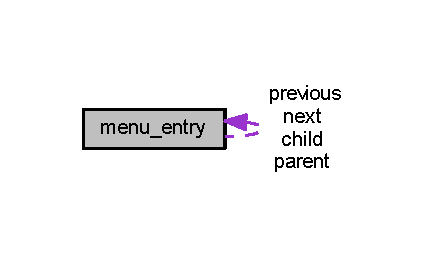
\includegraphics[width=214pt]{structmenu__entry__coll__graph}
\end{center}
\end{figure}
\subsection*{Datenfelder}
\begin{DoxyCompactItemize}
\item 
const struct \hyperlink{structmenu__entry}{menu\+\_\+entry} $\ast$ \hyperlink{structmenu__entry_a759c31dc71a94a9bbafdc849d2db5c1a}{child\+\_\+short}
\item 
const struct \hyperlink{structmenu__entry}{menu\+\_\+entry} $\ast$ \hyperlink{structmenu__entry_a79da8f2d51ac63708f7f8f41b56d0102}{child\+\_\+long}
\item 
const struct \hyperlink{structmenu__entry}{menu\+\_\+entry} $\ast$ \hyperlink{structmenu__entry_ac1b562fabcc9402003931e8351d6faf7}{parent}
\item 
const struct \hyperlink{structmenu__entry}{menu\+\_\+entry} $\ast$ \hyperlink{structmenu__entry_a8667330bb5cb56772e88abd901064211}{next}
\item 
const struct \hyperlink{structmenu__entry}{menu\+\_\+entry} $\ast$ \hyperlink{structmenu__entry_a66676e2c3f7553b50a8c1d0c4e973734}{previous}
\item 
const char $\ast$ \hyperlink{structmenu__entry_a16343090e80c4472521560f30113d96c}{text}
\item 
const uint16\+\_\+t \hyperlink{structmenu__entry_aead51ebe631627145d52a84b2d92e240}{entry\+\_\+num}
\end{DoxyCompactItemize}


\subsection{Ausführliche Beschreibung}


Definiert in Zeile 6 der Datei menu\+\_\+struct.\+h.



\subsection{Dokumentation der Datenelemente}
\hypertarget{structmenu__entry_a79da8f2d51ac63708f7f8f41b56d0102}{}\index{menu\+\_\+entry@{menu\+\_\+entry}!child\+\_\+long@{child\+\_\+long}}
\index{child\+\_\+long@{child\+\_\+long}!menu\+\_\+entry@{menu\+\_\+entry}}
\subsubsection[{child\+\_\+long}]{\setlength{\rightskip}{0pt plus 5cm}const struct {\bf menu\+\_\+entry}$\ast$ child\+\_\+long}\label{structmenu__entry_a79da8f2d51ac63708f7f8f41b56d0102}


Definiert in Zeile 8 der Datei menu\+\_\+struct.\+h.

\hypertarget{structmenu__entry_a759c31dc71a94a9bbafdc849d2db5c1a}{}\index{menu\+\_\+entry@{menu\+\_\+entry}!child\+\_\+short@{child\+\_\+short}}
\index{child\+\_\+short@{child\+\_\+short}!menu\+\_\+entry@{menu\+\_\+entry}}
\subsubsection[{child\+\_\+short}]{\setlength{\rightskip}{0pt plus 5cm}const struct {\bf menu\+\_\+entry}$\ast$ child\+\_\+short}\label{structmenu__entry_a759c31dc71a94a9bbafdc849d2db5c1a}


Definiert in Zeile 7 der Datei menu\+\_\+struct.\+h.

\hypertarget{structmenu__entry_aead51ebe631627145d52a84b2d92e240}{}\index{menu\+\_\+entry@{menu\+\_\+entry}!entry\+\_\+num@{entry\+\_\+num}}
\index{entry\+\_\+num@{entry\+\_\+num}!menu\+\_\+entry@{menu\+\_\+entry}}
\subsubsection[{entry\+\_\+num}]{\setlength{\rightskip}{0pt plus 5cm}const uint16\+\_\+t entry\+\_\+num}\label{structmenu__entry_aead51ebe631627145d52a84b2d92e240}


Definiert in Zeile 13 der Datei menu\+\_\+struct.\+h.

\hypertarget{structmenu__entry_a8667330bb5cb56772e88abd901064211}{}\index{menu\+\_\+entry@{menu\+\_\+entry}!next@{next}}
\index{next@{next}!menu\+\_\+entry@{menu\+\_\+entry}}
\subsubsection[{next}]{\setlength{\rightskip}{0pt plus 5cm}const struct {\bf menu\+\_\+entry}$\ast$ next}\label{structmenu__entry_a8667330bb5cb56772e88abd901064211}


Definiert in Zeile 10 der Datei menu\+\_\+struct.\+h.

\hypertarget{structmenu__entry_ac1b562fabcc9402003931e8351d6faf7}{}\index{menu\+\_\+entry@{menu\+\_\+entry}!parent@{parent}}
\index{parent@{parent}!menu\+\_\+entry@{menu\+\_\+entry}}
\subsubsection[{parent}]{\setlength{\rightskip}{0pt plus 5cm}const struct {\bf menu\+\_\+entry}$\ast$ parent}\label{structmenu__entry_ac1b562fabcc9402003931e8351d6faf7}


Definiert in Zeile 9 der Datei menu\+\_\+struct.\+h.

\hypertarget{structmenu__entry_a66676e2c3f7553b50a8c1d0c4e973734}{}\index{menu\+\_\+entry@{menu\+\_\+entry}!previous@{previous}}
\index{previous@{previous}!menu\+\_\+entry@{menu\+\_\+entry}}
\subsubsection[{previous}]{\setlength{\rightskip}{0pt plus 5cm}const struct {\bf menu\+\_\+entry}$\ast$ previous}\label{structmenu__entry_a66676e2c3f7553b50a8c1d0c4e973734}


Definiert in Zeile 11 der Datei menu\+\_\+struct.\+h.

\hypertarget{structmenu__entry_a16343090e80c4472521560f30113d96c}{}\index{menu\+\_\+entry@{menu\+\_\+entry}!text@{text}}
\index{text@{text}!menu\+\_\+entry@{menu\+\_\+entry}}
\subsubsection[{text}]{\setlength{\rightskip}{0pt plus 5cm}const char$\ast$ text}\label{structmenu__entry_a16343090e80c4472521560f30113d96c}


Definiert in Zeile 12 der Datei menu\+\_\+struct.\+h.



Die Dokumentation für diese Struktur wurde erzeugt aufgrund der Datei\+:\begin{DoxyCompactItemize}
\item 
menu/\hyperlink{menu__struct_8h}{menu\+\_\+struct.\+h}\end{DoxyCompactItemize}

\hypertarget{structopt3001__stc}{}\section{opt3001\+\_\+stc Strukturreferenz}
\label{structopt3001__stc}\index{opt3001\+\_\+stc@{opt3001\+\_\+stc}}


{\ttfamily \#include $<$opt3001.\+h$>$}

\subsection*{Datenfelder}
\begin{DoxyCompactItemize}
\item 
uint16\+\_\+t \hyperlink{structopt3001__stc_aa26297bc57b4b74262246d02175f4308}{config}
\item 
uint16\+\_\+t \hyperlink{structopt3001__stc_a5561e4eedc9af4ceb86ed5056241bf77}{low\+\_\+limit}
\item 
uint16\+\_\+t \hyperlink{structopt3001__stc_af121d4246e275920873b33ad155fa9ba}{high\+\_\+limit}
\end{DoxyCompactItemize}


\subsection{Ausführliche Beschreibung}


Definiert in Zeile 29 der Datei opt3001.\+h.



\subsection{Dokumentation der Datenelemente}
\hypertarget{structopt3001__stc_aa26297bc57b4b74262246d02175f4308}{}\index{opt3001\+\_\+stc@{opt3001\+\_\+stc}!config@{config}}
\index{config@{config}!opt3001\+\_\+stc@{opt3001\+\_\+stc}}
\subsubsection[{config}]{\setlength{\rightskip}{0pt plus 5cm}uint16\+\_\+t config}\label{structopt3001__stc_aa26297bc57b4b74262246d02175f4308}


Definiert in Zeile 30 der Datei opt3001.\+h.

\hypertarget{structopt3001__stc_af121d4246e275920873b33ad155fa9ba}{}\index{opt3001\+\_\+stc@{opt3001\+\_\+stc}!high\+\_\+limit@{high\+\_\+limit}}
\index{high\+\_\+limit@{high\+\_\+limit}!opt3001\+\_\+stc@{opt3001\+\_\+stc}}
\subsubsection[{high\+\_\+limit}]{\setlength{\rightskip}{0pt plus 5cm}uint16\+\_\+t high\+\_\+limit}\label{structopt3001__stc_af121d4246e275920873b33ad155fa9ba}


Definiert in Zeile 32 der Datei opt3001.\+h.

\hypertarget{structopt3001__stc_a5561e4eedc9af4ceb86ed5056241bf77}{}\index{opt3001\+\_\+stc@{opt3001\+\_\+stc}!low\+\_\+limit@{low\+\_\+limit}}
\index{low\+\_\+limit@{low\+\_\+limit}!opt3001\+\_\+stc@{opt3001\+\_\+stc}}
\subsubsection[{low\+\_\+limit}]{\setlength{\rightskip}{0pt plus 5cm}uint16\+\_\+t low\+\_\+limit}\label{structopt3001__stc_a5561e4eedc9af4ceb86ed5056241bf77}


Definiert in Zeile 31 der Datei opt3001.\+h.



Die Dokumentation für diese Struktur wurde erzeugt aufgrund der Datei\+:\begin{DoxyCompactItemize}
\item 
D\+:/\+G\+I\+T/fhradiov2/driver/\hyperlink{opt3001_8h}{opt3001.\+h}\end{DoxyCompactItemize}

\hypertarget{structpca9530}{}\section{pca9530 Strukturreferenz}
\label{structpca9530}\index{pca9530@{pca9530}}


{\ttfamily \#include $<$pca9530.\+h$>$}

\subsection*{Datenfelder}
\begin{DoxyCompactItemize}
\item 
uint8\+\_\+t \hyperlink{structpca9530_a1a85040128a35d94e73a6d6b96aea658}{freq0}
\item 
uint8\+\_\+t \hyperlink{structpca9530_a2fb4d580ed22ad326b72701b98038bdc}{pwm0}
\item 
uint8\+\_\+t \hyperlink{structpca9530_a05652b55717263bec9a0d63ff6690969}{freq1}
\item 
uint8\+\_\+t \hyperlink{structpca9530_af1f85784c51fc6b57b6e713d160e6136}{pwm1}
\item 
enum \hyperlink{pca9530_8h_ace2d36a1fc0cc58626736636eaff2237}{P\+C\+A9530\+\_\+\+L\+E\+D\+\_\+\+S\+T\+A\+T\+E} \hyperlink{structpca9530_a3a42a3267d245b293db10c2cbb3330f9}{led0}
\item 
enum \hyperlink{pca9530_8h_ace2d36a1fc0cc58626736636eaff2237}{P\+C\+A9530\+\_\+\+L\+E\+D\+\_\+\+S\+T\+A\+T\+E} \hyperlink{structpca9530_a3ac265af8bbeb022cd8ad2f21247f6ac}{led1}
\end{DoxyCompactItemize}


\subsection{Ausführliche Beschreibung}


Definiert in Zeile 64 der Datei pca9530.\+h.



\subsection{Dokumentation der Datenelemente}
\hypertarget{structpca9530_a1a85040128a35d94e73a6d6b96aea658}{}\index{pca9530@{pca9530}!freq0@{freq0}}
\index{freq0@{freq0}!pca9530@{pca9530}}
\subsubsection[{freq0}]{\setlength{\rightskip}{0pt plus 5cm}uint8\+\_\+t freq0}\label{structpca9530_a1a85040128a35d94e73a6d6b96aea658}


Definiert in Zeile 65 der Datei pca9530.\+h.

\hypertarget{structpca9530_a05652b55717263bec9a0d63ff6690969}{}\index{pca9530@{pca9530}!freq1@{freq1}}
\index{freq1@{freq1}!pca9530@{pca9530}}
\subsubsection[{freq1}]{\setlength{\rightskip}{0pt plus 5cm}uint8\+\_\+t freq1}\label{structpca9530_a05652b55717263bec9a0d63ff6690969}


Definiert in Zeile 67 der Datei pca9530.\+h.

\hypertarget{structpca9530_a3a42a3267d245b293db10c2cbb3330f9}{}\index{pca9530@{pca9530}!led0@{led0}}
\index{led0@{led0}!pca9530@{pca9530}}
\subsubsection[{led0}]{\setlength{\rightskip}{0pt plus 5cm}enum {\bf P\+C\+A9530\+\_\+\+L\+E\+D\+\_\+\+S\+T\+A\+T\+E} led0}\label{structpca9530_a3a42a3267d245b293db10c2cbb3330f9}


Definiert in Zeile 69 der Datei pca9530.\+h.

\hypertarget{structpca9530_a3ac265af8bbeb022cd8ad2f21247f6ac}{}\index{pca9530@{pca9530}!led1@{led1}}
\index{led1@{led1}!pca9530@{pca9530}}
\subsubsection[{led1}]{\setlength{\rightskip}{0pt plus 5cm}enum {\bf P\+C\+A9530\+\_\+\+L\+E\+D\+\_\+\+S\+T\+A\+T\+E} led1}\label{structpca9530_a3ac265af8bbeb022cd8ad2f21247f6ac}


Definiert in Zeile 70 der Datei pca9530.\+h.

\hypertarget{structpca9530_a2fb4d580ed22ad326b72701b98038bdc}{}\index{pca9530@{pca9530}!pwm0@{pwm0}}
\index{pwm0@{pwm0}!pca9530@{pca9530}}
\subsubsection[{pwm0}]{\setlength{\rightskip}{0pt plus 5cm}uint8\+\_\+t pwm0}\label{structpca9530_a2fb4d580ed22ad326b72701b98038bdc}


Definiert in Zeile 66 der Datei pca9530.\+h.

\hypertarget{structpca9530_af1f85784c51fc6b57b6e713d160e6136}{}\index{pca9530@{pca9530}!pwm1@{pwm1}}
\index{pwm1@{pwm1}!pca9530@{pca9530}}
\subsubsection[{pwm1}]{\setlength{\rightskip}{0pt plus 5cm}uint8\+\_\+t pwm1}\label{structpca9530_af1f85784c51fc6b57b6e713d160e6136}


Definiert in Zeile 68 der Datei pca9530.\+h.



Die Dokumentation für diese Struktur wurde erzeugt aufgrund der Datei\+:\begin{DoxyCompactItemize}
\item 
driver/\hyperlink{pca9530_8h}{pca9530.\+h}\end{DoxyCompactItemize}

\hypertarget{structpca9530__ctl}{}\section{pca9530\+\_\+ctl Strukturreferenz}
\label{structpca9530__ctl}\index{pca9530\+\_\+ctl@{pca9530\+\_\+ctl}}


{\ttfamily \#include $<$pca9530.\+h$>$}

\subsection*{Datenfelder}
\begin{DoxyCompactItemize}
\item 
uint8\+\_\+t \hyperlink{structpca9530__ctl_a8b4eebe79ded0459acec2f4950102ba3}{\+\_\+\+\_\+pad0\+\_\+\+\_\+}\+: 3
\item 
uint8\+\_\+t \hyperlink{structpca9530__ctl_a8782eaf4d6ff8b39d2ef058050c8a0e3}{A\+I}\+: 1
\item 
uint8\+\_\+t \hyperlink{structpca9530__ctl_a77f12d2e278bd5c07712648ac0df5e08}{\+\_\+\+\_\+pad1\+\_\+\+\_\+}\+: 1
\item 
uint8\+\_\+t \hyperlink{structpca9530__ctl_af3bea2c4759f3d001950aba2a1f89810}{A\+D\+D\+R\+E\+S\+S}\+: 3
\end{DoxyCompactItemize}


\subsection{Ausführliche Beschreibung}


Definiert in Zeile 45 der Datei pca9530.\+h.



\subsection{Dokumentation der Datenelemente}
\hypertarget{structpca9530__ctl_a8b4eebe79ded0459acec2f4950102ba3}{}\index{pca9530\+\_\+ctl@{pca9530\+\_\+ctl}!\+\_\+\+\_\+pad0\+\_\+\+\_\+@{\+\_\+\+\_\+pad0\+\_\+\+\_\+}}
\index{\+\_\+\+\_\+pad0\+\_\+\+\_\+@{\+\_\+\+\_\+pad0\+\_\+\+\_\+}!pca9530\+\_\+ctl@{pca9530\+\_\+ctl}}
\subsubsection[{\+\_\+\+\_\+pad0\+\_\+\+\_\+}]{\setlength{\rightskip}{0pt plus 5cm}uint8\+\_\+t \+\_\+\+\_\+pad0\+\_\+\+\_\+}\label{structpca9530__ctl_a8b4eebe79ded0459acec2f4950102ba3}


Definiert in Zeile 46 der Datei pca9530.\+h.

\hypertarget{structpca9530__ctl_a77f12d2e278bd5c07712648ac0df5e08}{}\index{pca9530\+\_\+ctl@{pca9530\+\_\+ctl}!\+\_\+\+\_\+pad1\+\_\+\+\_\+@{\+\_\+\+\_\+pad1\+\_\+\+\_\+}}
\index{\+\_\+\+\_\+pad1\+\_\+\+\_\+@{\+\_\+\+\_\+pad1\+\_\+\+\_\+}!pca9530\+\_\+ctl@{pca9530\+\_\+ctl}}
\subsubsection[{\+\_\+\+\_\+pad1\+\_\+\+\_\+}]{\setlength{\rightskip}{0pt plus 5cm}uint8\+\_\+t \+\_\+\+\_\+pad1\+\_\+\+\_\+}\label{structpca9530__ctl_a77f12d2e278bd5c07712648ac0df5e08}


Definiert in Zeile 48 der Datei pca9530.\+h.

\hypertarget{structpca9530__ctl_af3bea2c4759f3d001950aba2a1f89810}{}\index{pca9530\+\_\+ctl@{pca9530\+\_\+ctl}!A\+D\+D\+R\+E\+S\+S@{A\+D\+D\+R\+E\+S\+S}}
\index{A\+D\+D\+R\+E\+S\+S@{A\+D\+D\+R\+E\+S\+S}!pca9530\+\_\+ctl@{pca9530\+\_\+ctl}}
\subsubsection[{A\+D\+D\+R\+E\+S\+S}]{\setlength{\rightskip}{0pt plus 5cm}uint8\+\_\+t A\+D\+D\+R\+E\+S\+S}\label{structpca9530__ctl_af3bea2c4759f3d001950aba2a1f89810}


Definiert in Zeile 49 der Datei pca9530.\+h.

\hypertarget{structpca9530__ctl_a8782eaf4d6ff8b39d2ef058050c8a0e3}{}\index{pca9530\+\_\+ctl@{pca9530\+\_\+ctl}!A\+I@{A\+I}}
\index{A\+I@{A\+I}!pca9530\+\_\+ctl@{pca9530\+\_\+ctl}}
\subsubsection[{A\+I}]{\setlength{\rightskip}{0pt plus 5cm}uint8\+\_\+t A\+I}\label{structpca9530__ctl_a8782eaf4d6ff8b39d2ef058050c8a0e3}


Definiert in Zeile 47 der Datei pca9530.\+h.



Die Dokumentation für diese Struktur wurde erzeugt aufgrund der Datei\+:\begin{DoxyCompactItemize}
\item 
D\+:/\+G\+I\+T/fhradiov2/driver/\hyperlink{pca9530_8h}{pca9530.\+h}\end{DoxyCompactItemize}

\hypertarget{structpca9530__in}{}\section{pca9530\+\_\+in Strukturreferenz}
\label{structpca9530__in}\index{pca9530\+\_\+in@{pca9530\+\_\+in}}


{\ttfamily \#include $<$pca9530.\+h$>$}

\subsection*{Datenfelder}
\begin{DoxyCompactItemize}
\item 
uint8\+\_\+t \hyperlink{structpca9530__in_a8b4eebe79ded0459acec2f4950102ba3}{\+\_\+\+\_\+pad0\+\_\+\+\_\+}\+: 6
\item 
uint8\+\_\+t \hyperlink{structpca9530__in_a40e423e01a324e06ebc015b85a9d6b8e}{L\+E\+D1}\+: 1
\item 
uint8\+\_\+t \hyperlink{structpca9530__in_a698763138aab81826861fd602c87872b}{L\+E\+D0}\+: 1
\end{DoxyCompactItemize}


\subsection{Ausführliche Beschreibung}


Definiert in Zeile 52 der Datei pca9530.\+h.



\subsection{Dokumentation der Datenelemente}
\hypertarget{structpca9530__in_a8b4eebe79ded0459acec2f4950102ba3}{}\index{pca9530\+\_\+in@{pca9530\+\_\+in}!\+\_\+\+\_\+pad0\+\_\+\+\_\+@{\+\_\+\+\_\+pad0\+\_\+\+\_\+}}
\index{\+\_\+\+\_\+pad0\+\_\+\+\_\+@{\+\_\+\+\_\+pad0\+\_\+\+\_\+}!pca9530\+\_\+in@{pca9530\+\_\+in}}
\subsubsection[{\+\_\+\+\_\+pad0\+\_\+\+\_\+}]{\setlength{\rightskip}{0pt plus 5cm}uint8\+\_\+t \+\_\+\+\_\+pad0\+\_\+\+\_\+}\label{structpca9530__in_a8b4eebe79ded0459acec2f4950102ba3}


Definiert in Zeile 53 der Datei pca9530.\+h.

\hypertarget{structpca9530__in_a698763138aab81826861fd602c87872b}{}\index{pca9530\+\_\+in@{pca9530\+\_\+in}!L\+E\+D0@{L\+E\+D0}}
\index{L\+E\+D0@{L\+E\+D0}!pca9530\+\_\+in@{pca9530\+\_\+in}}
\subsubsection[{L\+E\+D0}]{\setlength{\rightskip}{0pt plus 5cm}uint8\+\_\+t L\+E\+D0}\label{structpca9530__in_a698763138aab81826861fd602c87872b}


Definiert in Zeile 55 der Datei pca9530.\+h.

\hypertarget{structpca9530__in_a40e423e01a324e06ebc015b85a9d6b8e}{}\index{pca9530\+\_\+in@{pca9530\+\_\+in}!L\+E\+D1@{L\+E\+D1}}
\index{L\+E\+D1@{L\+E\+D1}!pca9530\+\_\+in@{pca9530\+\_\+in}}
\subsubsection[{L\+E\+D1}]{\setlength{\rightskip}{0pt plus 5cm}uint8\+\_\+t L\+E\+D1}\label{structpca9530__in_a40e423e01a324e06ebc015b85a9d6b8e}


Definiert in Zeile 54 der Datei pca9530.\+h.



Die Dokumentation für diese Struktur wurde erzeugt aufgrund der Datei\+:\begin{DoxyCompactItemize}
\item 
D\+:/\+G\+I\+T/fhradiov2/driver/\hyperlink{pca9530_8h}{pca9530.\+h}\end{DoxyCompactItemize}

\hypertarget{structpca9530__sel}{}\section{pca9530\+\_\+sel Strukturreferenz}
\label{structpca9530__sel}\index{pca9530\+\_\+sel@{pca9530\+\_\+sel}}


{\ttfamily \#include $<$pca9530.\+h$>$}

\subsection*{Datenfelder}
\begin{DoxyCompactItemize}
\item 
uint8\+\_\+t \hyperlink{structpca9530__sel_a8b4eebe79ded0459acec2f4950102ba3}{\+\_\+\+\_\+pad0\+\_\+\+\_\+}\+: 4
\item 
uint8\+\_\+t \hyperlink{structpca9530__sel_a40e423e01a324e06ebc015b85a9d6b8e}{L\+E\+D1}\+: 2
\item 
uint8\+\_\+t \hyperlink{structpca9530__sel_a698763138aab81826861fd602c87872b}{L\+E\+D0}\+: 2
\end{DoxyCompactItemize}


\subsection{Ausführliche Beschreibung}


Definiert in Zeile 58 der Datei pca9530.\+h.



\subsection{Dokumentation der Datenelemente}
\hypertarget{structpca9530__sel_a8b4eebe79ded0459acec2f4950102ba3}{}\index{pca9530\+\_\+sel@{pca9530\+\_\+sel}!\+\_\+\+\_\+pad0\+\_\+\+\_\+@{\+\_\+\+\_\+pad0\+\_\+\+\_\+}}
\index{\+\_\+\+\_\+pad0\+\_\+\+\_\+@{\+\_\+\+\_\+pad0\+\_\+\+\_\+}!pca9530\+\_\+sel@{pca9530\+\_\+sel}}
\subsubsection[{\+\_\+\+\_\+pad0\+\_\+\+\_\+}]{\setlength{\rightskip}{0pt plus 5cm}uint8\+\_\+t \+\_\+\+\_\+pad0\+\_\+\+\_\+}\label{structpca9530__sel_a8b4eebe79ded0459acec2f4950102ba3}


Definiert in Zeile 59 der Datei pca9530.\+h.

\hypertarget{structpca9530__sel_a698763138aab81826861fd602c87872b}{}\index{pca9530\+\_\+sel@{pca9530\+\_\+sel}!L\+E\+D0@{L\+E\+D0}}
\index{L\+E\+D0@{L\+E\+D0}!pca9530\+\_\+sel@{pca9530\+\_\+sel}}
\subsubsection[{L\+E\+D0}]{\setlength{\rightskip}{0pt plus 5cm}uint8\+\_\+t L\+E\+D0}\label{structpca9530__sel_a698763138aab81826861fd602c87872b}


Definiert in Zeile 61 der Datei pca9530.\+h.

\hypertarget{structpca9530__sel_a40e423e01a324e06ebc015b85a9d6b8e}{}\index{pca9530\+\_\+sel@{pca9530\+\_\+sel}!L\+E\+D1@{L\+E\+D1}}
\index{L\+E\+D1@{L\+E\+D1}!pca9530\+\_\+sel@{pca9530\+\_\+sel}}
\subsubsection[{L\+E\+D1}]{\setlength{\rightskip}{0pt plus 5cm}uint8\+\_\+t L\+E\+D1}\label{structpca9530__sel_a40e423e01a324e06ebc015b85a9d6b8e}


Definiert in Zeile 60 der Datei pca9530.\+h.



Die Dokumentation für diese Struktur wurde erzeugt aufgrund der Datei\+:\begin{DoxyCompactItemize}
\item 
D\+:/\+G\+I\+T/fhradiov2/driver/\hyperlink{pca9530_8h}{pca9530.\+h}\end{DoxyCompactItemize}

\hypertarget{structpi}{}\section{pi Strukturreferenz}
\label{structpi}\index{pi@{pi}}


{\ttfamily \#include $<$rds.\+h$>$}

\subsection*{Datenfelder}
\begin{DoxyCompactItemize}
\item 
uint16\+\_\+t \hyperlink{structpi_aa0995bba54da782b6ff03d66f16e3c57}{P\+R\+O\+G\+R\+A\+M\+M\+\_\+\+R\+E\+F\+\_\+\+N\+U\+M}\+:8
\item 
uint16\+\_\+t \hyperlink{structpi_a71dba196e0ca59278a7cd48f95fd07f3}{A\+R\+E\+A\+\_\+\+C\+O\+D\+E}\+:4
\item 
uint16\+\_\+t \hyperlink{structpi_a104410f64e8aa7ab69f76a5ee53a0a8a}{C\+O\+U\+N\+T\+R\+Y\+\_\+\+C\+O\+D\+E}\+:4
\end{DoxyCompactItemize}


\subsection{Ausführliche Beschreibung}


Definiert in Zeile 156 der Datei rds.\+h.



\subsection{Dokumentation der Datenelemente}
\hypertarget{structpi_a71dba196e0ca59278a7cd48f95fd07f3}{}\index{pi@{pi}!A\+R\+E\+A\+\_\+\+C\+O\+D\+E@{A\+R\+E\+A\+\_\+\+C\+O\+D\+E}}
\index{A\+R\+E\+A\+\_\+\+C\+O\+D\+E@{A\+R\+E\+A\+\_\+\+C\+O\+D\+E}!pi@{pi}}
\subsubsection[{A\+R\+E\+A\+\_\+\+C\+O\+D\+E}]{\setlength{\rightskip}{0pt plus 5cm}uint16\+\_\+t A\+R\+E\+A\+\_\+\+C\+O\+D\+E}\label{structpi_a71dba196e0ca59278a7cd48f95fd07f3}


Definiert in Zeile 158 der Datei rds.\+h.

\hypertarget{structpi_a104410f64e8aa7ab69f76a5ee53a0a8a}{}\index{pi@{pi}!C\+O\+U\+N\+T\+R\+Y\+\_\+\+C\+O\+D\+E@{C\+O\+U\+N\+T\+R\+Y\+\_\+\+C\+O\+D\+E}}
\index{C\+O\+U\+N\+T\+R\+Y\+\_\+\+C\+O\+D\+E@{C\+O\+U\+N\+T\+R\+Y\+\_\+\+C\+O\+D\+E}!pi@{pi}}
\subsubsection[{C\+O\+U\+N\+T\+R\+Y\+\_\+\+C\+O\+D\+E}]{\setlength{\rightskip}{0pt plus 5cm}uint16\+\_\+t C\+O\+U\+N\+T\+R\+Y\+\_\+\+C\+O\+D\+E}\label{structpi_a104410f64e8aa7ab69f76a5ee53a0a8a}


Definiert in Zeile 159 der Datei rds.\+h.

\hypertarget{structpi_aa0995bba54da782b6ff03d66f16e3c57}{}\index{pi@{pi}!P\+R\+O\+G\+R\+A\+M\+M\+\_\+\+R\+E\+F\+\_\+\+N\+U\+M@{P\+R\+O\+G\+R\+A\+M\+M\+\_\+\+R\+E\+F\+\_\+\+N\+U\+M}}
\index{P\+R\+O\+G\+R\+A\+M\+M\+\_\+\+R\+E\+F\+\_\+\+N\+U\+M@{P\+R\+O\+G\+R\+A\+M\+M\+\_\+\+R\+E\+F\+\_\+\+N\+U\+M}!pi@{pi}}
\subsubsection[{P\+R\+O\+G\+R\+A\+M\+M\+\_\+\+R\+E\+F\+\_\+\+N\+U\+M}]{\setlength{\rightskip}{0pt plus 5cm}uint16\+\_\+t P\+R\+O\+G\+R\+A\+M\+M\+\_\+\+R\+E\+F\+\_\+\+N\+U\+M}\label{structpi_aa0995bba54da782b6ff03d66f16e3c57}


Definiert in Zeile 157 der Datei rds.\+h.



Die Dokumentation für diese Struktur wurde erzeugt aufgrund der Datei\+:\begin{DoxyCompactItemize}
\item 
system/\hyperlink{rds_8h}{rds.\+h}\end{DoxyCompactItemize}

\hypertarget{unionpower__up__arg1}{}\section{power\+\_\+up\+\_\+arg1 Variantenreferenz}
\label{unionpower__up__arg1}\index{power\+\_\+up\+\_\+arg1@{power\+\_\+up\+\_\+arg1}}


{\ttfamily \#include $<$si4735\+\_\+cmd\+\_\+prop.\+h$>$}

\subsection*{Datenfelder}
\begin{DoxyCompactItemize}
\item 
uint8\+\_\+t \hyperlink{unionpower__up__arg1_a96f44d20f1dbf1c8785a7bc99a46164c}{byte}
\item 
\begin{tabbing}
xx\=xx\=xx\=xx\=xx\=xx\=xx\=xx\=xx\=\kill
struct \{\\
\>uint8\_t \hyperlink{unionpower__up__arg1_a4454e61ca41936d70ce251c7aa931f60}{CTSIEN}:1\\
\>uint8\_t \hyperlink{unionpower__up__arg1_aa16577946f684dfeeee75c5552b2cf32}{GPO2OEN}:1\\
\>uint8\_t \hyperlink{unionpower__up__arg1_aa2fc9067222815bec88b0dc6048b2956}{PATCH}:1\\
\>uint8\_t \hyperlink{unionpower__up__arg1_a56b7fb7e7e5dfc8eed9d066f71579077}{XOSCEN}:1\\
\>uint8\_t \hyperlink{unionpower__up__arg1_a0aab01836b450d01cbad756334c65fab}{FUNC}:4\\
\}; \\

\end{tabbing}\end{DoxyCompactItemize}


\subsection{Ausführliche Beschreibung}


Definiert in Zeile 36 der Datei si4735\+\_\+cmd\+\_\+prop.\+h.



\subsection{Dokumentation der Datenelemente}
\hypertarget{unionpower__up__arg1_ab3d22615500b3bd400498c7e667f8684}{}\subsubsection[{"@3}]{\setlength{\rightskip}{0pt plus 5cm}struct \{ ... \} }\label{unionpower__up__arg1_ab3d22615500b3bd400498c7e667f8684}
\hypertarget{unionpower__up__arg1_a96f44d20f1dbf1c8785a7bc99a46164c}{}\index{power\+\_\+up\+\_\+arg1@{power\+\_\+up\+\_\+arg1}!byte@{byte}}
\index{byte@{byte}!power\+\_\+up\+\_\+arg1@{power\+\_\+up\+\_\+arg1}}
\subsubsection[{byte}]{\setlength{\rightskip}{0pt plus 5cm}uint8\+\_\+t byte}\label{unionpower__up__arg1_a96f44d20f1dbf1c8785a7bc99a46164c}


Definiert in Zeile 37 der Datei si4735\+\_\+cmd\+\_\+prop.\+h.

\hypertarget{unionpower__up__arg1_a4454e61ca41936d70ce251c7aa931f60}{}\index{power\+\_\+up\+\_\+arg1@{power\+\_\+up\+\_\+arg1}!C\+T\+S\+I\+E\+N@{C\+T\+S\+I\+E\+N}}
\index{C\+T\+S\+I\+E\+N@{C\+T\+S\+I\+E\+N}!power\+\_\+up\+\_\+arg1@{power\+\_\+up\+\_\+arg1}}
\subsubsection[{C\+T\+S\+I\+E\+N}]{\setlength{\rightskip}{0pt plus 5cm}uint8\+\_\+t C\+T\+S\+I\+E\+N}\label{unionpower__up__arg1_a4454e61ca41936d70ce251c7aa931f60}


Definiert in Zeile 39 der Datei si4735\+\_\+cmd\+\_\+prop.\+h.

\hypertarget{unionpower__up__arg1_a0aab01836b450d01cbad756334c65fab}{}\index{power\+\_\+up\+\_\+arg1@{power\+\_\+up\+\_\+arg1}!F\+U\+N\+C@{F\+U\+N\+C}}
\index{F\+U\+N\+C@{F\+U\+N\+C}!power\+\_\+up\+\_\+arg1@{power\+\_\+up\+\_\+arg1}}
\subsubsection[{F\+U\+N\+C}]{\setlength{\rightskip}{0pt plus 5cm}uint8\+\_\+t F\+U\+N\+C}\label{unionpower__up__arg1_a0aab01836b450d01cbad756334c65fab}


Definiert in Zeile 43 der Datei si4735\+\_\+cmd\+\_\+prop.\+h.

\hypertarget{unionpower__up__arg1_aa16577946f684dfeeee75c5552b2cf32}{}\index{power\+\_\+up\+\_\+arg1@{power\+\_\+up\+\_\+arg1}!G\+P\+O2\+O\+E\+N@{G\+P\+O2\+O\+E\+N}}
\index{G\+P\+O2\+O\+E\+N@{G\+P\+O2\+O\+E\+N}!power\+\_\+up\+\_\+arg1@{power\+\_\+up\+\_\+arg1}}
\subsubsection[{G\+P\+O2\+O\+E\+N}]{\setlength{\rightskip}{0pt plus 5cm}uint8\+\_\+t G\+P\+O2\+O\+E\+N}\label{unionpower__up__arg1_aa16577946f684dfeeee75c5552b2cf32}


Definiert in Zeile 40 der Datei si4735\+\_\+cmd\+\_\+prop.\+h.

\hypertarget{unionpower__up__arg1_aa2fc9067222815bec88b0dc6048b2956}{}\index{power\+\_\+up\+\_\+arg1@{power\+\_\+up\+\_\+arg1}!P\+A\+T\+C\+H@{P\+A\+T\+C\+H}}
\index{P\+A\+T\+C\+H@{P\+A\+T\+C\+H}!power\+\_\+up\+\_\+arg1@{power\+\_\+up\+\_\+arg1}}
\subsubsection[{P\+A\+T\+C\+H}]{\setlength{\rightskip}{0pt plus 5cm}uint8\+\_\+t P\+A\+T\+C\+H}\label{unionpower__up__arg1_aa2fc9067222815bec88b0dc6048b2956}


Definiert in Zeile 41 der Datei si4735\+\_\+cmd\+\_\+prop.\+h.

\hypertarget{unionpower__up__arg1_a56b7fb7e7e5dfc8eed9d066f71579077}{}\index{power\+\_\+up\+\_\+arg1@{power\+\_\+up\+\_\+arg1}!X\+O\+S\+C\+E\+N@{X\+O\+S\+C\+E\+N}}
\index{X\+O\+S\+C\+E\+N@{X\+O\+S\+C\+E\+N}!power\+\_\+up\+\_\+arg1@{power\+\_\+up\+\_\+arg1}}
\subsubsection[{X\+O\+S\+C\+E\+N}]{\setlength{\rightskip}{0pt plus 5cm}uint8\+\_\+t X\+O\+S\+C\+E\+N}\label{unionpower__up__arg1_a56b7fb7e7e5dfc8eed9d066f71579077}


Definiert in Zeile 42 der Datei si4735\+\_\+cmd\+\_\+prop.\+h.



Die Dokumentation für diese Variante wurde erzeugt aufgrund der Datei\+:\begin{DoxyCompactItemize}
\item 
driver/include/\hyperlink{si4735__cmd__prop_8h}{si4735\+\_\+cmd\+\_\+prop.\+h}\end{DoxyCompactItemize}

\hypertarget{structradio}{}\section{radio Strukturreferenz}
\label{structradio}\index{radio@{radio}}


{\ttfamily \#include $<$radio.\+h$>$}



Zusammengehörigkeiten von radio\+:\nopagebreak
\begin{figure}[H]
\begin{center}
\leavevmode
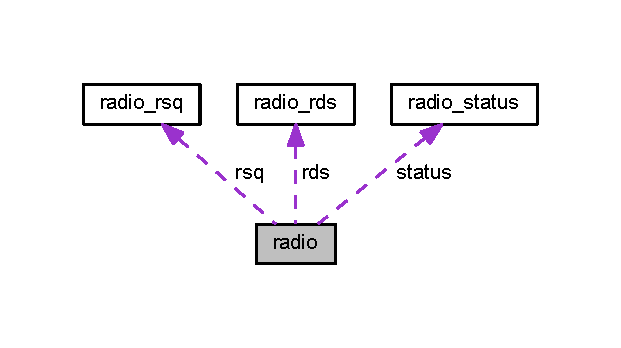
\includegraphics[width=298pt]{structradio__coll__graph}
\end{center}
\end{figure}
\subsection*{Datenfelder}
\begin{DoxyCompactItemize}
\item 
uint16\+\_\+t \hyperlink{structradio_ae9e2de5c2a6d31fe02952daeb7d0f2cc}{station\+\_\+freq}
\item 
int8\+\_\+t \hyperlink{structradio_a0fe6eefa6e7f7329eb95938b5802289a}{volume}
\item 
uint8\+\_\+t \hyperlink{structradio_a837c871f200f8c3d19d0c7f2e031ffc4}{brightness}
\item 
uint8\+\_\+t \hyperlink{structradio_a1498c49a1583af22b892d695900a74db}{contrast}
\item 
\hyperlink{radio_8h_a903525b4070dadc3575c79be7341f94c}{R\+A\+D\+I\+O\+\_\+\+S\+T\+A\+T\+U\+S} \hyperlink{structradio_ac40df2ac7cfc276418e34335098903fb}{status}
\item 
\hyperlink{radio_8h_a45097f726be0f44e9afecd5102888dbd}{R\+A\+D\+I\+O\+\_\+\+R\+D\+S} \hyperlink{structradio_a44efb20f93a5de661983c36b4a870f4e}{rds}
\item 
\hyperlink{radio_8h_ab4334359915ce423f1ca752a4384a70f}{R\+A\+D\+I\+O\+\_\+\+R\+S\+Q} \hyperlink{structradio_aba45ded08c975dcc6ee7d58687e8534e}{rsq}
\end{DoxyCompactItemize}


\subsection{Ausführliche Beschreibung}


Definiert in Zeile 61 der Datei radio.\+h.



\subsection{Dokumentation der Datenelemente}
\hypertarget{structradio_a837c871f200f8c3d19d0c7f2e031ffc4}{}\index{radio@{radio}!brightness@{brightness}}
\index{brightness@{brightness}!radio@{radio}}
\subsubsection[{brightness}]{\setlength{\rightskip}{0pt plus 5cm}uint8\+\_\+t brightness}\label{structradio_a837c871f200f8c3d19d0c7f2e031ffc4}


Definiert in Zeile 64 der Datei radio.\+h.

\hypertarget{structradio_a1498c49a1583af22b892d695900a74db}{}\index{radio@{radio}!contrast@{contrast}}
\index{contrast@{contrast}!radio@{radio}}
\subsubsection[{contrast}]{\setlength{\rightskip}{0pt plus 5cm}uint8\+\_\+t contrast}\label{structradio_a1498c49a1583af22b892d695900a74db}


Definiert in Zeile 65 der Datei radio.\+h.

\hypertarget{structradio_a44efb20f93a5de661983c36b4a870f4e}{}\index{radio@{radio}!rds@{rds}}
\index{rds@{rds}!radio@{radio}}
\subsubsection[{rds}]{\setlength{\rightskip}{0pt plus 5cm}{\bf R\+A\+D\+I\+O\+\_\+\+R\+D\+S} {\bf rds}}\label{structradio_a44efb20f93a5de661983c36b4a870f4e}


Definiert in Zeile 67 der Datei radio.\+h.

\hypertarget{structradio_aba45ded08c975dcc6ee7d58687e8534e}{}\index{radio@{radio}!rsq@{rsq}}
\index{rsq@{rsq}!radio@{radio}}
\subsubsection[{rsq}]{\setlength{\rightskip}{0pt plus 5cm}{\bf R\+A\+D\+I\+O\+\_\+\+R\+S\+Q} rsq}\label{structradio_aba45ded08c975dcc6ee7d58687e8534e}


Definiert in Zeile 68 der Datei radio.\+h.

\hypertarget{structradio_ae9e2de5c2a6d31fe02952daeb7d0f2cc}{}\index{radio@{radio}!station\+\_\+freq@{station\+\_\+freq}}
\index{station\+\_\+freq@{station\+\_\+freq}!radio@{radio}}
\subsubsection[{station\+\_\+freq}]{\setlength{\rightskip}{0pt plus 5cm}uint16\+\_\+t station\+\_\+freq}\label{structradio_ae9e2de5c2a6d31fe02952daeb7d0f2cc}


Definiert in Zeile 62 der Datei radio.\+h.

\hypertarget{structradio_ac40df2ac7cfc276418e34335098903fb}{}\index{radio@{radio}!status@{status}}
\index{status@{status}!radio@{radio}}
\subsubsection[{status}]{\setlength{\rightskip}{0pt plus 5cm}{\bf R\+A\+D\+I\+O\+\_\+\+S\+T\+A\+T\+U\+S} {\bf status}}\label{structradio_ac40df2ac7cfc276418e34335098903fb}


Definiert in Zeile 66 der Datei radio.\+h.

\hypertarget{structradio_a0fe6eefa6e7f7329eb95938b5802289a}{}\index{radio@{radio}!volume@{volume}}
\index{volume@{volume}!radio@{radio}}
\subsubsection[{volume}]{\setlength{\rightskip}{0pt plus 5cm}int8\+\_\+t volume}\label{structradio_a0fe6eefa6e7f7329eb95938b5802289a}


Definiert in Zeile 63 der Datei radio.\+h.



Die Dokumentation für diese Struktur wurde erzeugt aufgrund der Datei\+:\begin{DoxyCompactItemize}
\item 
system/\hyperlink{radio_8h}{radio.\+h}\end{DoxyCompactItemize}

\hypertarget{structradio__rds}{}\section{radio\+\_\+rds Strukturreferenz}
\label{structradio__rds}\index{radio\+\_\+rds@{radio\+\_\+rds}}


{\ttfamily \#include $<$radio.\+h$>$}

\subsection*{Datenfelder}
\begin{DoxyCompactItemize}
\item 
char \hyperlink{structradio__rds_a00c5e915306c0baea463b99ba6c09c4f}{name} \mbox{[}9\mbox{]}
\item 
char \hyperlink{structradio__rds_a1d7cd4d36a6a2fa49631cef5d5847187}{text} \mbox{[}65\mbox{]}
\item 
uint16\+\_\+t \hyperlink{structradio__rds_ad1803744db28ac0d226ec8da9134598e}{pi}
\item 
uint16\+\_\+t \hyperlink{structradio__rds_a6a555813c441b0e0dce51020817fa68e}{pty}\+:5
\item 
uint16\+\_\+t \hyperlink{structradio__rds_aaa7c4cc5a934d489d475d0f7d26e437c}{ta}\+:1
\item 
uint16\+\_\+t \hyperlink{structradio__rds_a92aabb0ca71171ea02dd5cf0ada0d536}{tp}\+:1
\item 
uint16\+\_\+t \hyperlink{structradio__rds_a8d03256977e8f265177523adc9bab6c0}{ms}\+:1
\item 
uint16\+\_\+t \hyperlink{structradio__rds_aaea7b514ca0c80db1989dc43cf4fe3c1}{di}\+:4
\end{DoxyCompactItemize}


\subsection{Ausführliche Beschreibung}


Definiert in Zeile 102 der Datei radio.\+h.



\subsection{Dokumentation der Datenelemente}
\hypertarget{structradio__rds_aaea7b514ca0c80db1989dc43cf4fe3c1}{}\index{radio\+\_\+rds@{radio\+\_\+rds}!di@{di}}
\index{di@{di}!radio\+\_\+rds@{radio\+\_\+rds}}
\subsubsection[{di}]{\setlength{\rightskip}{0pt plus 5cm}uint16\+\_\+t di}\label{structradio__rds_aaea7b514ca0c80db1989dc43cf4fe3c1}


Definiert in Zeile 110 der Datei radio.\+h.

\hypertarget{structradio__rds_a8d03256977e8f265177523adc9bab6c0}{}\index{radio\+\_\+rds@{radio\+\_\+rds}!ms@{ms}}
\index{ms@{ms}!radio\+\_\+rds@{radio\+\_\+rds}}
\subsubsection[{ms}]{\setlength{\rightskip}{0pt plus 5cm}uint16\+\_\+t ms}\label{structradio__rds_a8d03256977e8f265177523adc9bab6c0}


Definiert in Zeile 109 der Datei radio.\+h.

\hypertarget{structradio__rds_a00c5e915306c0baea463b99ba6c09c4f}{}\index{radio\+\_\+rds@{radio\+\_\+rds}!name@{name}}
\index{name@{name}!radio\+\_\+rds@{radio\+\_\+rds}}
\subsubsection[{name}]{\setlength{\rightskip}{0pt plus 5cm}char name\mbox{[}9\mbox{]}}\label{structradio__rds_a00c5e915306c0baea463b99ba6c09c4f}


Definiert in Zeile 103 der Datei radio.\+h.

\hypertarget{structradio__rds_ad1803744db28ac0d226ec8da9134598e}{}\index{radio\+\_\+rds@{radio\+\_\+rds}!pi@{pi}}
\index{pi@{pi}!radio\+\_\+rds@{radio\+\_\+rds}}
\subsubsection[{pi}]{\setlength{\rightskip}{0pt plus 5cm}uint16\+\_\+t pi}\label{structradio__rds_ad1803744db28ac0d226ec8da9134598e}


Definiert in Zeile 105 der Datei radio.\+h.

\hypertarget{structradio__rds_a6a555813c441b0e0dce51020817fa68e}{}\index{radio\+\_\+rds@{radio\+\_\+rds}!pty@{pty}}
\index{pty@{pty}!radio\+\_\+rds@{radio\+\_\+rds}}
\subsubsection[{pty}]{\setlength{\rightskip}{0pt plus 5cm}uint16\+\_\+t pty}\label{structradio__rds_a6a555813c441b0e0dce51020817fa68e}


Definiert in Zeile 106 der Datei radio.\+h.

\hypertarget{structradio__rds_aaa7c4cc5a934d489d475d0f7d26e437c}{}\index{radio\+\_\+rds@{radio\+\_\+rds}!ta@{ta}}
\index{ta@{ta}!radio\+\_\+rds@{radio\+\_\+rds}}
\subsubsection[{ta}]{\setlength{\rightskip}{0pt plus 5cm}uint16\+\_\+t ta}\label{structradio__rds_aaa7c4cc5a934d489d475d0f7d26e437c}


Definiert in Zeile 107 der Datei radio.\+h.

\hypertarget{structradio__rds_a1d7cd4d36a6a2fa49631cef5d5847187}{}\index{radio\+\_\+rds@{radio\+\_\+rds}!text@{text}}
\index{text@{text}!radio\+\_\+rds@{radio\+\_\+rds}}
\subsubsection[{text}]{\setlength{\rightskip}{0pt plus 5cm}char text\mbox{[}65\mbox{]}}\label{structradio__rds_a1d7cd4d36a6a2fa49631cef5d5847187}


Definiert in Zeile 104 der Datei radio.\+h.

\hypertarget{structradio__rds_a92aabb0ca71171ea02dd5cf0ada0d536}{}\index{radio\+\_\+rds@{radio\+\_\+rds}!tp@{tp}}
\index{tp@{tp}!radio\+\_\+rds@{radio\+\_\+rds}}
\subsubsection[{tp}]{\setlength{\rightskip}{0pt plus 5cm}uint16\+\_\+t tp}\label{structradio__rds_a92aabb0ca71171ea02dd5cf0ada0d536}


Definiert in Zeile 108 der Datei radio.\+h.



Die Dokumentation für diese Struktur wurde erzeugt aufgrund der Datei\+:\begin{DoxyCompactItemize}
\item 
D\+:/\+G\+I\+T/fhradiov2/system/\hyperlink{radio_8h}{radio.\+h}\end{DoxyCompactItemize}

\hypertarget{structradio__rsq}{}\section{radio\+\_\+rsq Strukturreferenz}
\label{structradio__rsq}\index{radio\+\_\+rsq@{radio\+\_\+rsq}}


{\ttfamily \#include $<$radio.\+h$>$}

\subsection*{Datenfelder}
\begin{DoxyCompactItemize}
\item 
uint8\+\_\+t \hyperlink{structradio__rsq_afb67d818cd76cce8057affabcb1979a6}{rssi}
\item 
uint8\+\_\+t \hyperlink{structradio__rsq_a11be3c6f2d5194542e5d1733cbc7ac76}{snr}
\item 
uint8\+\_\+t \hyperlink{structradio__rsq_af829dbd700d1c5ad1abccbdb52fa7ba9}{multi}
\item 
int8\+\_\+t \hyperlink{structradio__rsq_a168a73926de154445f6c6c77f8b5e53c}{freq\+\_\+off}
\end{DoxyCompactItemize}


\subsection{Ausführliche Beschreibung}


Definiert in Zeile 73 der Datei radio.\+h.



\subsection{Dokumentation der Datenelemente}
\hypertarget{structradio__rsq_a168a73926de154445f6c6c77f8b5e53c}{}\index{radio\+\_\+rsq@{radio\+\_\+rsq}!freq\+\_\+off@{freq\+\_\+off}}
\index{freq\+\_\+off@{freq\+\_\+off}!radio\+\_\+rsq@{radio\+\_\+rsq}}
\subsubsection[{freq\+\_\+off}]{\setlength{\rightskip}{0pt plus 5cm}int8\+\_\+t freq\+\_\+off}\label{structradio__rsq_a168a73926de154445f6c6c77f8b5e53c}


Definiert in Zeile 77 der Datei radio.\+h.

\hypertarget{structradio__rsq_af829dbd700d1c5ad1abccbdb52fa7ba9}{}\index{radio\+\_\+rsq@{radio\+\_\+rsq}!multi@{multi}}
\index{multi@{multi}!radio\+\_\+rsq@{radio\+\_\+rsq}}
\subsubsection[{multi}]{\setlength{\rightskip}{0pt plus 5cm}uint8\+\_\+t multi}\label{structradio__rsq_af829dbd700d1c5ad1abccbdb52fa7ba9}


Definiert in Zeile 76 der Datei radio.\+h.

\hypertarget{structradio__rsq_afb67d818cd76cce8057affabcb1979a6}{}\index{radio\+\_\+rsq@{radio\+\_\+rsq}!rssi@{rssi}}
\index{rssi@{rssi}!radio\+\_\+rsq@{radio\+\_\+rsq}}
\subsubsection[{rssi}]{\setlength{\rightskip}{0pt plus 5cm}uint8\+\_\+t rssi}\label{structradio__rsq_afb67d818cd76cce8057affabcb1979a6}


Definiert in Zeile 74 der Datei radio.\+h.

\hypertarget{structradio__rsq_a11be3c6f2d5194542e5d1733cbc7ac76}{}\index{radio\+\_\+rsq@{radio\+\_\+rsq}!snr@{snr}}
\index{snr@{snr}!radio\+\_\+rsq@{radio\+\_\+rsq}}
\subsubsection[{snr}]{\setlength{\rightskip}{0pt plus 5cm}uint8\+\_\+t snr}\label{structradio__rsq_a11be3c6f2d5194542e5d1733cbc7ac76}


Definiert in Zeile 75 der Datei radio.\+h.



Die Dokumentation für diese Struktur wurde erzeugt aufgrund der Datei\+:\begin{DoxyCompactItemize}
\item 
D\+:/\+G\+I\+T/fhradiov2/radio/\hyperlink{radio_8h}{radio.\+h}\end{DoxyCompactItemize}

\hypertarget{structradio__status}{}\section{radio\+\_\+status Strukturreferenz}
\label{structradio__status}\index{radio\+\_\+status@{radio\+\_\+status}}


{\ttfamily \#include $<$radio.\+h$>$}

\subsection*{Datenfelder}
\begin{DoxyCompactItemize}
\item 
uint16\+\_\+t \hyperlink{structradio__status_a5b532af663903e8196d7781d3f6767e3}{station\+\_\+valid}\+:1
\item 
uint16\+\_\+t \hyperlink{structradio__status_aa4b556b7564cd5016a39e2a5c3aab1b9}{text\+\_\+valid}\+:1
\item 
uint16\+\_\+t \hyperlink{structradio__status_a3d873f4f8e8dd5c6dcc0c930a44c3449}{time\+\_\+valid}\+:1
\item 
uint16\+\_\+t \hyperlink{structradio__status_a842d6e1b68c63972c4c4e968b1cb3ecc}{name\+\_\+valid}\+:1
\item 
uint16\+\_\+t \hyperlink{structradio__status_a978bf90e15e81e6bd50889aa0df2c7ce}{freq\+\_\+valid}\+:1
\item 
uint16\+\_\+t \hyperlink{structradio__status_aac214d01bdfc63d8cc9c8ec2e870068b}{scroll\+\_\+text}\+:4
\item 
uint16\+\_\+t \hyperlink{structradio__status_a2adcc7027dfa4863cdf990071f08a141}{display\+\_\+mode}\+:2
\item 
uint16\+\_\+t \hyperlink{structradio__status_a89c0ce618dc30ac07daea694a9ec664e}{audio\+\_\+mute}\+:1
\item 
uint16\+\_\+t \hyperlink{structradio__status_a77132c2c26a75f5b8751b235cda23828}{\+\_\+\+\_\+pad0\+\_\+\+\_\+}\+:4
\end{DoxyCompactItemize}


\subsection{Ausführliche Beschreibung}


Definiert in Zeile 35 der Datei radio.\+h.



\subsection{Dokumentation der Datenelemente}
\hypertarget{structradio__status_a77132c2c26a75f5b8751b235cda23828}{}\index{radio\+\_\+status@{radio\+\_\+status}!\+\_\+\+\_\+pad0\+\_\+\+\_\+@{\+\_\+\+\_\+pad0\+\_\+\+\_\+}}
\index{\+\_\+\+\_\+pad0\+\_\+\+\_\+@{\+\_\+\+\_\+pad0\+\_\+\+\_\+}!radio\+\_\+status@{radio\+\_\+status}}
\subsubsection[{\+\_\+\+\_\+pad0\+\_\+\+\_\+}]{\setlength{\rightskip}{0pt plus 5cm}uint16\+\_\+t \+\_\+\+\_\+pad0\+\_\+\+\_\+}\label{structradio__status_a77132c2c26a75f5b8751b235cda23828}


Definiert in Zeile 44 der Datei radio.\+h.

\hypertarget{structradio__status_a89c0ce618dc30ac07daea694a9ec664e}{}\index{radio\+\_\+status@{radio\+\_\+status}!audio\+\_\+mute@{audio\+\_\+mute}}
\index{audio\+\_\+mute@{audio\+\_\+mute}!radio\+\_\+status@{radio\+\_\+status}}
\subsubsection[{audio\+\_\+mute}]{\setlength{\rightskip}{0pt plus 5cm}uint16\+\_\+t audio\+\_\+mute}\label{structradio__status_a89c0ce618dc30ac07daea694a9ec664e}


Definiert in Zeile 43 der Datei radio.\+h.

\hypertarget{structradio__status_a2adcc7027dfa4863cdf990071f08a141}{}\index{radio\+\_\+status@{radio\+\_\+status}!display\+\_\+mode@{display\+\_\+mode}}
\index{display\+\_\+mode@{display\+\_\+mode}!radio\+\_\+status@{radio\+\_\+status}}
\subsubsection[{display\+\_\+mode}]{\setlength{\rightskip}{0pt plus 5cm}uint16\+\_\+t display\+\_\+mode}\label{structradio__status_a2adcc7027dfa4863cdf990071f08a141}


Definiert in Zeile 42 der Datei radio.\+h.

\hypertarget{structradio__status_a978bf90e15e81e6bd50889aa0df2c7ce}{}\index{radio\+\_\+status@{radio\+\_\+status}!freq\+\_\+valid@{freq\+\_\+valid}}
\index{freq\+\_\+valid@{freq\+\_\+valid}!radio\+\_\+status@{radio\+\_\+status}}
\subsubsection[{freq\+\_\+valid}]{\setlength{\rightskip}{0pt plus 5cm}uint16\+\_\+t freq\+\_\+valid}\label{structradio__status_a978bf90e15e81e6bd50889aa0df2c7ce}


Definiert in Zeile 40 der Datei radio.\+h.

\hypertarget{structradio__status_a842d6e1b68c63972c4c4e968b1cb3ecc}{}\index{radio\+\_\+status@{radio\+\_\+status}!name\+\_\+valid@{name\+\_\+valid}}
\index{name\+\_\+valid@{name\+\_\+valid}!radio\+\_\+status@{radio\+\_\+status}}
\subsubsection[{name\+\_\+valid}]{\setlength{\rightskip}{0pt plus 5cm}uint16\+\_\+t name\+\_\+valid}\label{structradio__status_a842d6e1b68c63972c4c4e968b1cb3ecc}


Definiert in Zeile 39 der Datei radio.\+h.

\hypertarget{structradio__status_aac214d01bdfc63d8cc9c8ec2e870068b}{}\index{radio\+\_\+status@{radio\+\_\+status}!scroll\+\_\+text@{scroll\+\_\+text}}
\index{scroll\+\_\+text@{scroll\+\_\+text}!radio\+\_\+status@{radio\+\_\+status}}
\subsubsection[{scroll\+\_\+text}]{\setlength{\rightskip}{0pt plus 5cm}uint16\+\_\+t scroll\+\_\+text}\label{structradio__status_aac214d01bdfc63d8cc9c8ec2e870068b}


Definiert in Zeile 41 der Datei radio.\+h.

\hypertarget{structradio__status_a5b532af663903e8196d7781d3f6767e3}{}\index{radio\+\_\+status@{radio\+\_\+status}!station\+\_\+valid@{station\+\_\+valid}}
\index{station\+\_\+valid@{station\+\_\+valid}!radio\+\_\+status@{radio\+\_\+status}}
\subsubsection[{station\+\_\+valid}]{\setlength{\rightskip}{0pt plus 5cm}uint16\+\_\+t station\+\_\+valid}\label{structradio__status_a5b532af663903e8196d7781d3f6767e3}


Definiert in Zeile 36 der Datei radio.\+h.

\hypertarget{structradio__status_aa4b556b7564cd5016a39e2a5c3aab1b9}{}\index{radio\+\_\+status@{radio\+\_\+status}!text\+\_\+valid@{text\+\_\+valid}}
\index{text\+\_\+valid@{text\+\_\+valid}!radio\+\_\+status@{radio\+\_\+status}}
\subsubsection[{text\+\_\+valid}]{\setlength{\rightskip}{0pt plus 5cm}uint16\+\_\+t text\+\_\+valid}\label{structradio__status_aa4b556b7564cd5016a39e2a5c3aab1b9}


Definiert in Zeile 37 der Datei radio.\+h.

\hypertarget{structradio__status_a3d873f4f8e8dd5c6dcc0c930a44c3449}{}\index{radio\+\_\+status@{radio\+\_\+status}!time\+\_\+valid@{time\+\_\+valid}}
\index{time\+\_\+valid@{time\+\_\+valid}!radio\+\_\+status@{radio\+\_\+status}}
\subsubsection[{time\+\_\+valid}]{\setlength{\rightskip}{0pt plus 5cm}uint16\+\_\+t time\+\_\+valid}\label{structradio__status_a3d873f4f8e8dd5c6dcc0c930a44c3449}


Definiert in Zeile 38 der Datei radio.\+h.



Die Dokumentation für diese Struktur wurde erzeugt aufgrund der Datei\+:\begin{DoxyCompactItemize}
\item 
system/\hyperlink{radio_8h}{radio.\+h}\end{DoxyCompactItemize}

\hypertarget{structrds}{}\section{rds Strukturreferenz}
\label{structrds}\index{rds@{rds}}


{\ttfamily \#include $<$rds.\+h$>$}



Zusammengehörigkeiten von rds\+:
\nopagebreak
\begin{figure}[H]
\begin{center}
\leavevmode
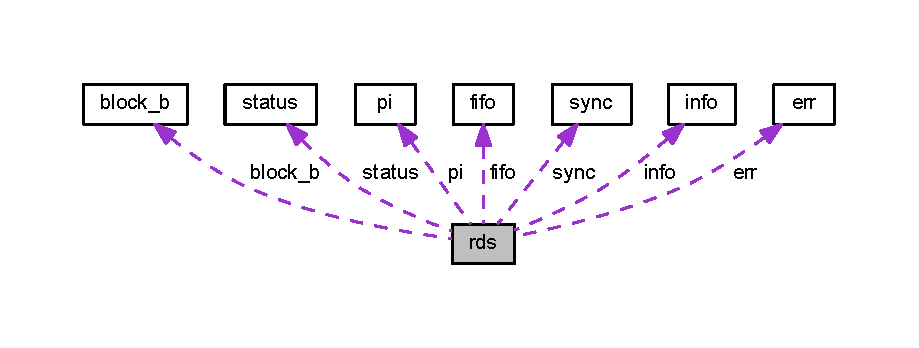
\includegraphics[width=350pt]{structrds__coll__graph}
\end{center}
\end{figure}
\subsection*{Datenfelder}
\begin{DoxyCompactItemize}
\item 
\hyperlink{rds_8h_ada2ef00c464f9ae8ec73e127ea6a4520}{S\+T\+A\+T\+U\+S} \hyperlink{structrds_a1025e6cbbd3179d2d91b9b4afb8f8efc}{status}
\item 
\hyperlink{rds_8h_a4d0cac7fd06c1f9b01c6a67516c95cfb}{I\+N\+F\+O} \hyperlink{structrds_a8936b68dc62d34c0bd4298d71e811a89}{info}
\item 
\hyperlink{rds_8h_a09f25e919a775a5955c4fb87155e2762}{S\+Y\+N\+C} \hyperlink{structrds_aa779e41fc5dcd8e1471033612c290b23}{sync}
\item 
\hyperlink{rds_8h_a632395f1ea2941b14cb3baef84705059}{F\+I\+F\+O} \hyperlink{structrds_a7f4b3988a39d63bbb74e44a08285d9ef}{fifo}
\item 
uint16\+\_\+t \hyperlink{structrds_ad1803744db28ac0d226ec8da9134598e}{pi}
\item 
\hyperlink{rds_8h_acde5bba1b29ae92f2d1c088cbc0e40bd}{B\+L\+O\+C\+K\+\_\+\+B} \hyperlink{structrds_ad8c59b1a87492b568b0bf85aef6f5f87}{block\+\_\+b}
\item 
uint8\+\_\+t \hyperlink{structrds_af966591bcdc65611d3f9ec47cd36d52a}{block} \mbox{[}4\mbox{]}
\item 
\hyperlink{rds_8h_aa7225a8602f1106cb23bf648d85efb2c}{E\+R\+R} \hyperlink{structrds_a533130a85d028e42078891666dd6c6fc}{err}
\end{DoxyCompactItemize}


\subsection{Ausführliche Beschreibung}


Definiert in Zeile 163 der Datei rds.\+h.



\subsection{Dokumentation der Datenelemente}
\hypertarget{structrds_af966591bcdc65611d3f9ec47cd36d52a}{}\index{rds@{rds}!block@{block}}
\index{block@{block}!rds@{rds}}
\subsubsection[{block}]{\setlength{\rightskip}{0pt plus 5cm}uint8\+\_\+t block\mbox{[}4\mbox{]}}\label{structrds_af966591bcdc65611d3f9ec47cd36d52a}


Definiert in Zeile 170 der Datei rds.\+h.

\hypertarget{structrds_ad8c59b1a87492b568b0bf85aef6f5f87}{}\index{rds@{rds}!block\+\_\+b@{block\+\_\+b}}
\index{block\+\_\+b@{block\+\_\+b}!rds@{rds}}
\subsubsection[{block\+\_\+b}]{\setlength{\rightskip}{0pt plus 5cm}{\bf B\+L\+O\+C\+K\+\_\+\+B} {\bf block\+\_\+b}}\label{structrds_ad8c59b1a87492b568b0bf85aef6f5f87}


Definiert in Zeile 169 der Datei rds.\+h.

\hypertarget{structrds_a533130a85d028e42078891666dd6c6fc}{}\index{rds@{rds}!err@{err}}
\index{err@{err}!rds@{rds}}
\subsubsection[{err}]{\setlength{\rightskip}{0pt plus 5cm}{\bf E\+R\+R} {\bf err}}\label{structrds_a533130a85d028e42078891666dd6c6fc}


Definiert in Zeile 171 der Datei rds.\+h.

\hypertarget{structrds_a7f4b3988a39d63bbb74e44a08285d9ef}{}\index{rds@{rds}!fifo@{fifo}}
\index{fifo@{fifo}!rds@{rds}}
\subsubsection[{fifo}]{\setlength{\rightskip}{0pt plus 5cm}{\bf F\+I\+F\+O} {\bf fifo}}\label{structrds_a7f4b3988a39d63bbb74e44a08285d9ef}


Definiert in Zeile 167 der Datei rds.\+h.

\hypertarget{structrds_a8936b68dc62d34c0bd4298d71e811a89}{}\index{rds@{rds}!info@{info}}
\index{info@{info}!rds@{rds}}
\subsubsection[{info}]{\setlength{\rightskip}{0pt plus 5cm}{\bf I\+N\+F\+O} {\bf info}}\label{structrds_a8936b68dc62d34c0bd4298d71e811a89}


Definiert in Zeile 165 der Datei rds.\+h.

\hypertarget{structrds_ad1803744db28ac0d226ec8da9134598e}{}\index{rds@{rds}!pi@{pi}}
\index{pi@{pi}!rds@{rds}}
\subsubsection[{pi}]{\setlength{\rightskip}{0pt plus 5cm}uint16\+\_\+t pi}\label{structrds_ad1803744db28ac0d226ec8da9134598e}


Definiert in Zeile 168 der Datei rds.\+h.

\hypertarget{structrds_a1025e6cbbd3179d2d91b9b4afb8f8efc}{}\index{rds@{rds}!status@{status}}
\index{status@{status}!rds@{rds}}
\subsubsection[{status}]{\setlength{\rightskip}{0pt plus 5cm}{\bf S\+T\+A\+T\+U\+S} {\bf status}}\label{structrds_a1025e6cbbd3179d2d91b9b4afb8f8efc}


Definiert in Zeile 164 der Datei rds.\+h.

\hypertarget{structrds_aa779e41fc5dcd8e1471033612c290b23}{}\index{rds@{rds}!sync@{sync}}
\index{sync@{sync}!rds@{rds}}
\subsubsection[{sync}]{\setlength{\rightskip}{0pt plus 5cm}{\bf S\+Y\+N\+C} {\bf sync}}\label{structrds_aa779e41fc5dcd8e1471033612c290b23}


Definiert in Zeile 166 der Datei rds.\+h.



Die Dokumentation für diese Struktur wurde erzeugt aufgrund der Datei\+:\begin{DoxyCompactItemize}
\item 
D\+:/\+G\+I\+T/fhradiov2/system/\hyperlink{rds_8h}{rds.\+h}\end{DoxyCompactItemize}

\hypertarget{unionrefclk__pre}{}\section{refclk\+\_\+pre Variantenreferenz}
\label{unionrefclk__pre}\index{refclk\+\_\+pre@{refclk\+\_\+pre}}


{\ttfamily \#include $<$si4735\+\_\+cmd\+\_\+prop.\+h$>$}

\subsection*{Datenfelder}
\begin{DoxyCompactItemize}
\item 
uint16\+\_\+t \hyperlink{unionrefclk__pre_ab0549c1b5ea980a02e7eab77e21fea49}{byte}
\item 
uint8\+\_\+t \hyperlink{unionrefclk__pre_a46e4c05d20a047ec169f60d3167e912e}{bytes} \mbox{[}2\mbox{]}
\item 
\begin{tabbing}
xx\=xx\=xx\=xx\=xx\=xx\=xx\=xx\=xx\=\kill
struct \{\\
\>uint16\_t \hyperlink{unionrefclk__pre_a77132c2c26a75f5b8751b235cda23828}{\_\_pad0\_\_}:3\\
\>\>{\em Reserved. }\\
\>uint16\_t \hyperlink{unionrefclk__pre_a58f70e82912101800a780a4e8d24345d}{RCLKSEL}:1\\
\>uint16\_t \hyperlink{unionrefclk__pre_a546b4baeb928274149bafc12e1b720ff}{REFCLKP}:12\\
\}; \\

\end{tabbing}\end{DoxyCompactItemize}


\subsection{Ausführliche Beschreibung}


Definiert in Zeile 437 der Datei si4735\+\_\+cmd\+\_\+prop.\+h.



\subsection{Dokumentation der Datenelemente}
\hypertarget{unionrefclk__pre_a3e0747646412a75f934730c22ac67d34}{}\subsubsection[{"@45}]{\setlength{\rightskip}{0pt plus 5cm}struct \{ ... \} }\label{unionrefclk__pre_a3e0747646412a75f934730c22ac67d34}
\hypertarget{unionrefclk__pre_a77132c2c26a75f5b8751b235cda23828}{}\index{refclk\+\_\+pre@{refclk\+\_\+pre}!\+\_\+\+\_\+pad0\+\_\+\+\_\+@{\+\_\+\+\_\+pad0\+\_\+\+\_\+}}
\index{\+\_\+\+\_\+pad0\+\_\+\+\_\+@{\+\_\+\+\_\+pad0\+\_\+\+\_\+}!refclk\+\_\+pre@{refclk\+\_\+pre}}
\subsubsection[{\+\_\+\+\_\+pad0\+\_\+\+\_\+}]{\setlength{\rightskip}{0pt plus 5cm}uint16\+\_\+t \+\_\+\+\_\+pad0\+\_\+\+\_\+}\label{unionrefclk__pre_a77132c2c26a75f5b8751b235cda23828}


Reserved. 



Definiert in Zeile 441 der Datei si4735\+\_\+cmd\+\_\+prop.\+h.

\hypertarget{unionrefclk__pre_ab0549c1b5ea980a02e7eab77e21fea49}{}\index{refclk\+\_\+pre@{refclk\+\_\+pre}!byte@{byte}}
\index{byte@{byte}!refclk\+\_\+pre@{refclk\+\_\+pre}}
\subsubsection[{byte}]{\setlength{\rightskip}{0pt plus 5cm}uint16\+\_\+t byte}\label{unionrefclk__pre_ab0549c1b5ea980a02e7eab77e21fea49}


Definiert in Zeile 438 der Datei si4735\+\_\+cmd\+\_\+prop.\+h.

\hypertarget{unionrefclk__pre_a46e4c05d20a047ec169f60d3167e912e}{}\index{refclk\+\_\+pre@{refclk\+\_\+pre}!bytes@{bytes}}
\index{bytes@{bytes}!refclk\+\_\+pre@{refclk\+\_\+pre}}
\subsubsection[{bytes}]{\setlength{\rightskip}{0pt plus 5cm}uint8\+\_\+t bytes\mbox{[}2\mbox{]}}\label{unionrefclk__pre_a46e4c05d20a047ec169f60d3167e912e}


Definiert in Zeile 439 der Datei si4735\+\_\+cmd\+\_\+prop.\+h.

\hypertarget{unionrefclk__pre_a58f70e82912101800a780a4e8d24345d}{}\index{refclk\+\_\+pre@{refclk\+\_\+pre}!R\+C\+L\+K\+S\+E\+L@{R\+C\+L\+K\+S\+E\+L}}
\index{R\+C\+L\+K\+S\+E\+L@{R\+C\+L\+K\+S\+E\+L}!refclk\+\_\+pre@{refclk\+\_\+pre}}
\subsubsection[{R\+C\+L\+K\+S\+E\+L}]{\setlength{\rightskip}{0pt plus 5cm}uint16\+\_\+t R\+C\+L\+K\+S\+E\+L}\label{unionrefclk__pre_a58f70e82912101800a780a4e8d24345d}


Definiert in Zeile 442 der Datei si4735\+\_\+cmd\+\_\+prop.\+h.

\hypertarget{unionrefclk__pre_a546b4baeb928274149bafc12e1b720ff}{}\index{refclk\+\_\+pre@{refclk\+\_\+pre}!R\+E\+F\+C\+L\+K\+P@{R\+E\+F\+C\+L\+K\+P}}
\index{R\+E\+F\+C\+L\+K\+P@{R\+E\+F\+C\+L\+K\+P}!refclk\+\_\+pre@{refclk\+\_\+pre}}
\subsubsection[{R\+E\+F\+C\+L\+K\+P}]{\setlength{\rightskip}{0pt plus 5cm}uint16\+\_\+t R\+E\+F\+C\+L\+K\+P}\label{unionrefclk__pre_a546b4baeb928274149bafc12e1b720ff}


Definiert in Zeile 443 der Datei si4735\+\_\+cmd\+\_\+prop.\+h.



Die Dokumentation für diese Variante wurde erzeugt aufgrund der Datei\+:\begin{DoxyCompactItemize}
\item 
D\+:/\+G\+I\+T/fhradiov2/driver/include/\hyperlink{si4735__cmd__prop_8h}{si4735\+\_\+cmd\+\_\+prop.\+h}\end{DoxyCompactItemize}

\hypertarget{unionrx__hard__mute}{}\section{rx\+\_\+hard\+\_\+mute Variantenreferenz}
\label{unionrx__hard__mute}\index{rx\+\_\+hard\+\_\+mute@{rx\+\_\+hard\+\_\+mute}}


{\ttfamily \#include $<$si4735\+\_\+cmd\+\_\+prop.\+h$>$}

\subsection*{Datenfelder}
\begin{DoxyCompactItemize}
\item 
uint16\+\_\+t \hyperlink{unionrx__hard__mute_ab0549c1b5ea980a02e7eab77e21fea49}{byte}
\item 
uint8\+\_\+t \hyperlink{unionrx__hard__mute_a46e4c05d20a047ec169f60d3167e912e}{bytes} \mbox{[}2\mbox{]}
\item 
\begin{tabbing}
xx\=xx\=xx\=xx\=xx\=xx\=xx\=xx\=xx\=\kill
struct \{\\
\>uint16\_t \hyperlink{unionrx__hard__mute_a77132c2c26a75f5b8751b235cda23828}{\_\_pad0\_\_}:14\\
\>uint16\_t \hyperlink{unionrx__hard__mute_af01ca9e8c674119ab743ec7a084a56b3}{LMUTE}:1\\
\>uint16\_t \hyperlink{unionrx__hard__mute_a21b48010c5f26c6dc60ad46364bc10a0}{RMUTE}:1\\
\}; \\

\end{tabbing}\end{DoxyCompactItemize}


\subsection{Ausführliche Beschreibung}


Definiert in Zeile 1055 der Datei si4735\+\_\+cmd\+\_\+prop.\+h.



\subsection{Dokumentation der Datenelemente}
\hypertarget{unionrx__hard__mute_a40d7ad45a15f7efc8dbda66dff220270}{}\subsubsection[{"@129}]{\setlength{\rightskip}{0pt plus 5cm}struct \{ ... \} }\label{unionrx__hard__mute_a40d7ad45a15f7efc8dbda66dff220270}
\hypertarget{unionrx__hard__mute_a77132c2c26a75f5b8751b235cda23828}{}\index{rx\+\_\+hard\+\_\+mute@{rx\+\_\+hard\+\_\+mute}!\+\_\+\+\_\+pad0\+\_\+\+\_\+@{\+\_\+\+\_\+pad0\+\_\+\+\_\+}}
\index{\+\_\+\+\_\+pad0\+\_\+\+\_\+@{\+\_\+\+\_\+pad0\+\_\+\+\_\+}!rx\+\_\+hard\+\_\+mute@{rx\+\_\+hard\+\_\+mute}}
\subsubsection[{\+\_\+\+\_\+pad0\+\_\+\+\_\+}]{\setlength{\rightskip}{0pt plus 5cm}uint16\+\_\+t \+\_\+\+\_\+pad0\+\_\+\+\_\+}\label{unionrx__hard__mute_a77132c2c26a75f5b8751b235cda23828}


Definiert in Zeile 1059 der Datei si4735\+\_\+cmd\+\_\+prop.\+h.

\hypertarget{unionrx__hard__mute_ab0549c1b5ea980a02e7eab77e21fea49}{}\index{rx\+\_\+hard\+\_\+mute@{rx\+\_\+hard\+\_\+mute}!byte@{byte}}
\index{byte@{byte}!rx\+\_\+hard\+\_\+mute@{rx\+\_\+hard\+\_\+mute}}
\subsubsection[{byte}]{\setlength{\rightskip}{0pt plus 5cm}uint16\+\_\+t byte}\label{unionrx__hard__mute_ab0549c1b5ea980a02e7eab77e21fea49}


Definiert in Zeile 1056 der Datei si4735\+\_\+cmd\+\_\+prop.\+h.

\hypertarget{unionrx__hard__mute_a46e4c05d20a047ec169f60d3167e912e}{}\index{rx\+\_\+hard\+\_\+mute@{rx\+\_\+hard\+\_\+mute}!bytes@{bytes}}
\index{bytes@{bytes}!rx\+\_\+hard\+\_\+mute@{rx\+\_\+hard\+\_\+mute}}
\subsubsection[{bytes}]{\setlength{\rightskip}{0pt plus 5cm}uint8\+\_\+t bytes\mbox{[}2\mbox{]}}\label{unionrx__hard__mute_a46e4c05d20a047ec169f60d3167e912e}


Definiert in Zeile 1057 der Datei si4735\+\_\+cmd\+\_\+prop.\+h.

\hypertarget{unionrx__hard__mute_af01ca9e8c674119ab743ec7a084a56b3}{}\index{rx\+\_\+hard\+\_\+mute@{rx\+\_\+hard\+\_\+mute}!L\+M\+U\+T\+E@{L\+M\+U\+T\+E}}
\index{L\+M\+U\+T\+E@{L\+M\+U\+T\+E}!rx\+\_\+hard\+\_\+mute@{rx\+\_\+hard\+\_\+mute}}
\subsubsection[{L\+M\+U\+T\+E}]{\setlength{\rightskip}{0pt plus 5cm}uint16\+\_\+t L\+M\+U\+T\+E}\label{unionrx__hard__mute_af01ca9e8c674119ab743ec7a084a56b3}


Definiert in Zeile 1060 der Datei si4735\+\_\+cmd\+\_\+prop.\+h.

\hypertarget{unionrx__hard__mute_a21b48010c5f26c6dc60ad46364bc10a0}{}\index{rx\+\_\+hard\+\_\+mute@{rx\+\_\+hard\+\_\+mute}!R\+M\+U\+T\+E@{R\+M\+U\+T\+E}}
\index{R\+M\+U\+T\+E@{R\+M\+U\+T\+E}!rx\+\_\+hard\+\_\+mute@{rx\+\_\+hard\+\_\+mute}}
\subsubsection[{R\+M\+U\+T\+E}]{\setlength{\rightskip}{0pt plus 5cm}uint16\+\_\+t R\+M\+U\+T\+E}\label{unionrx__hard__mute_a21b48010c5f26c6dc60ad46364bc10a0}


Definiert in Zeile 1061 der Datei si4735\+\_\+cmd\+\_\+prop.\+h.



Die Dokumentation für diese Variante wurde erzeugt aufgrund der Datei\+:\begin{DoxyCompactItemize}
\item 
driver/include/\hyperlink{si4735__cmd__prop_8h}{si4735\+\_\+cmd\+\_\+prop.\+h}\end{DoxyCompactItemize}

\hypertarget{unionrx__volume}{}\section{rx\+\_\+volume Variantenreferenz}
\label{unionrx__volume}\index{rx\+\_\+volume@{rx\+\_\+volume}}


{\ttfamily \#include $<$si4735\+\_\+cmd\+\_\+prop.\+h$>$}

\subsection*{Datenfelder}
\begin{DoxyCompactItemize}
\item 
uint16\+\_\+t \hyperlink{unionrx__volume_ab0549c1b5ea980a02e7eab77e21fea49}{byte}
\item 
uint8\+\_\+t \hyperlink{unionrx__volume_a46e4c05d20a047ec169f60d3167e912e}{bytes} \mbox{[}2\mbox{]}
\item 
\begin{tabbing}
xx\=xx\=xx\=xx\=xx\=xx\=xx\=xx\=xx\=\kill
struct \{\\
\>uint16\_t \hyperlink{unionrx__volume_a77132c2c26a75f5b8751b235cda23828}{\_\_pad0\_\_}:10\\
\>uint16\_t \hyperlink{unionrx__volume_a03739146af570e536bfcb72ec21ffee9}{VOLUME}:6\\
\}; \\

\end{tabbing}\end{DoxyCompactItemize}


\subsection{Ausführliche Beschreibung}


Definiert in Zeile 1043 der Datei si4735\+\_\+cmd\+\_\+prop.\+h.



\subsection{Dokumentation der Datenelemente}
\hypertarget{unionrx__volume_a835c10068d0c39aad72ac3320be819d4}{}\subsubsection[{"@127}]{\setlength{\rightskip}{0pt plus 5cm}struct \{ ... \} }\label{unionrx__volume_a835c10068d0c39aad72ac3320be819d4}
\hypertarget{unionrx__volume_a77132c2c26a75f5b8751b235cda23828}{}\index{rx\+\_\+volume@{rx\+\_\+volume}!\+\_\+\+\_\+pad0\+\_\+\+\_\+@{\+\_\+\+\_\+pad0\+\_\+\+\_\+}}
\index{\+\_\+\+\_\+pad0\+\_\+\+\_\+@{\+\_\+\+\_\+pad0\+\_\+\+\_\+}!rx\+\_\+volume@{rx\+\_\+volume}}
\subsubsection[{\+\_\+\+\_\+pad0\+\_\+\+\_\+}]{\setlength{\rightskip}{0pt plus 5cm}uint16\+\_\+t \+\_\+\+\_\+pad0\+\_\+\+\_\+}\label{unionrx__volume_a77132c2c26a75f5b8751b235cda23828}


Definiert in Zeile 1047 der Datei si4735\+\_\+cmd\+\_\+prop.\+h.

\hypertarget{unionrx__volume_ab0549c1b5ea980a02e7eab77e21fea49}{}\index{rx\+\_\+volume@{rx\+\_\+volume}!byte@{byte}}
\index{byte@{byte}!rx\+\_\+volume@{rx\+\_\+volume}}
\subsubsection[{byte}]{\setlength{\rightskip}{0pt plus 5cm}uint16\+\_\+t byte}\label{unionrx__volume_ab0549c1b5ea980a02e7eab77e21fea49}


Definiert in Zeile 1044 der Datei si4735\+\_\+cmd\+\_\+prop.\+h.

\hypertarget{unionrx__volume_a46e4c05d20a047ec169f60d3167e912e}{}\index{rx\+\_\+volume@{rx\+\_\+volume}!bytes@{bytes}}
\index{bytes@{bytes}!rx\+\_\+volume@{rx\+\_\+volume}}
\subsubsection[{bytes}]{\setlength{\rightskip}{0pt plus 5cm}uint8\+\_\+t bytes\mbox{[}2\mbox{]}}\label{unionrx__volume_a46e4c05d20a047ec169f60d3167e912e}


Definiert in Zeile 1045 der Datei si4735\+\_\+cmd\+\_\+prop.\+h.

\hypertarget{unionrx__volume_a03739146af570e536bfcb72ec21ffee9}{}\index{rx\+\_\+volume@{rx\+\_\+volume}!V\+O\+L\+U\+M\+E@{V\+O\+L\+U\+M\+E}}
\index{V\+O\+L\+U\+M\+E@{V\+O\+L\+U\+M\+E}!rx\+\_\+volume@{rx\+\_\+volume}}
\subsubsection[{V\+O\+L\+U\+M\+E}]{\setlength{\rightskip}{0pt plus 5cm}uint16\+\_\+t V\+O\+L\+U\+M\+E}\label{unionrx__volume_a03739146af570e536bfcb72ec21ffee9}


Definiert in Zeile 1048 der Datei si4735\+\_\+cmd\+\_\+prop.\+h.



Die Dokumentation für diese Variante wurde erzeugt aufgrund der Datei\+:\begin{DoxyCompactItemize}
\item 
driver/include/\hyperlink{si4735__cmd__prop_8h}{si4735\+\_\+cmd\+\_\+prop.\+h}\end{DoxyCompactItemize}

\hypertarget{structstatus}{}\section{status Strukturreferenz}
\label{structstatus}\index{status@{status}}


In here the are structs declared for several R\+D\+S stuff(See \href{http://www.g.laroche}{\tt http\+://www.\+g.\+laroche}. free.\+fr/english/rds/groupes/liste\+Groupes\+R\+D\+S.htm for more information). Also there are functions declared to update R\+D\+S and to get the current time out of R\+D\+S.  




{\ttfamily \#include $<$rds.\+h$>$}

\subsection*{Datenfelder}
\begin{DoxyCompactItemize}
\item 
uint8\+\_\+t \hyperlink{structstatus_a1026d3a63b328db2451abc49e0bd5a2c}{S\+T\+C\+I\+N\+T}\+:1
\item 
uint8\+\_\+t \hyperlink{structstatus_a8b4eebe79ded0459acec2f4950102ba3}{\+\_\+\+\_\+pad0\+\_\+\+\_\+}\+:1
\item 
uint8\+\_\+t \hyperlink{structstatus_a4fac7351844086822dbf634529f6cfbd}{R\+D\+S\+I\+N\+T}\+:1
\item 
uint8\+\_\+t \hyperlink{structstatus_a9637ec0bb6d40570ea68a1b96c5d561e}{R\+S\+Q\+I\+N\+T}\+:1
\item 
uint8\+\_\+t \hyperlink{structstatus_a77f12d2e278bd5c07712648ac0df5e08}{\+\_\+\+\_\+pad1\+\_\+\+\_\+}\+:2
\item 
uint8\+\_\+t \hyperlink{structstatus_afb74dff3cfacd68c02883e5282ef2f59}{E\+R\+R}\+:1
\item 
uint8\+\_\+t \hyperlink{structstatus_a7f1760325354f291b9a0190e7e355ca8}{C\+T\+S}\+:1
\end{DoxyCompactItemize}


\subsection{Ausführliche Beschreibung}
In here the are structs declared for several R\+D\+S stuff(See \href{http://www.g.laroche}{\tt http\+://www.\+g.\+laroche}. free.\+fr/english/rds/groupes/liste\+Groupes\+R\+D\+S.htm for more information). Also there are functions declared to update R\+D\+S and to get the current time out of R\+D\+S. 

Definiert in Zeile 29 der Datei rds.\+h.



\subsection{Dokumentation der Datenelemente}
\hypertarget{structstatus_a8b4eebe79ded0459acec2f4950102ba3}{}\index{status@{status}!\+\_\+\+\_\+pad0\+\_\+\+\_\+@{\+\_\+\+\_\+pad0\+\_\+\+\_\+}}
\index{\+\_\+\+\_\+pad0\+\_\+\+\_\+@{\+\_\+\+\_\+pad0\+\_\+\+\_\+}!status@{status}}
\subsubsection[{\+\_\+\+\_\+pad0\+\_\+\+\_\+}]{\setlength{\rightskip}{0pt plus 5cm}uint8\+\_\+t \+\_\+\+\_\+pad0\+\_\+\+\_\+}\label{structstatus_a8b4eebe79ded0459acec2f4950102ba3}


Definiert in Zeile 31 der Datei rds.\+h.

\hypertarget{structstatus_a77f12d2e278bd5c07712648ac0df5e08}{}\index{status@{status}!\+\_\+\+\_\+pad1\+\_\+\+\_\+@{\+\_\+\+\_\+pad1\+\_\+\+\_\+}}
\index{\+\_\+\+\_\+pad1\+\_\+\+\_\+@{\+\_\+\+\_\+pad1\+\_\+\+\_\+}!status@{status}}
\subsubsection[{\+\_\+\+\_\+pad1\+\_\+\+\_\+}]{\setlength{\rightskip}{0pt plus 5cm}uint8\+\_\+t \+\_\+\+\_\+pad1\+\_\+\+\_\+}\label{structstatus_a77f12d2e278bd5c07712648ac0df5e08}


Definiert in Zeile 34 der Datei rds.\+h.

\hypertarget{structstatus_a7f1760325354f291b9a0190e7e355ca8}{}\index{status@{status}!C\+T\+S@{C\+T\+S}}
\index{C\+T\+S@{C\+T\+S}!status@{status}}
\subsubsection[{C\+T\+S}]{\setlength{\rightskip}{0pt plus 5cm}uint8\+\_\+t C\+T\+S}\label{structstatus_a7f1760325354f291b9a0190e7e355ca8}


Definiert in Zeile 36 der Datei rds.\+h.

\hypertarget{structstatus_afb74dff3cfacd68c02883e5282ef2f59}{}\index{status@{status}!E\+R\+R@{E\+R\+R}}
\index{E\+R\+R@{E\+R\+R}!status@{status}}
\subsubsection[{E\+R\+R}]{\setlength{\rightskip}{0pt plus 5cm}uint8\+\_\+t {\bf E\+R\+R}}\label{structstatus_afb74dff3cfacd68c02883e5282ef2f59}


Definiert in Zeile 35 der Datei rds.\+h.

\hypertarget{structstatus_a4fac7351844086822dbf634529f6cfbd}{}\index{status@{status}!R\+D\+S\+I\+N\+T@{R\+D\+S\+I\+N\+T}}
\index{R\+D\+S\+I\+N\+T@{R\+D\+S\+I\+N\+T}!status@{status}}
\subsubsection[{R\+D\+S\+I\+N\+T}]{\setlength{\rightskip}{0pt plus 5cm}uint8\+\_\+t R\+D\+S\+I\+N\+T}\label{structstatus_a4fac7351844086822dbf634529f6cfbd}


Definiert in Zeile 32 der Datei rds.\+h.

\hypertarget{structstatus_a9637ec0bb6d40570ea68a1b96c5d561e}{}\index{status@{status}!R\+S\+Q\+I\+N\+T@{R\+S\+Q\+I\+N\+T}}
\index{R\+S\+Q\+I\+N\+T@{R\+S\+Q\+I\+N\+T}!status@{status}}
\subsubsection[{R\+S\+Q\+I\+N\+T}]{\setlength{\rightskip}{0pt plus 5cm}uint8\+\_\+t R\+S\+Q\+I\+N\+T}\label{structstatus_a9637ec0bb6d40570ea68a1b96c5d561e}


Definiert in Zeile 33 der Datei rds.\+h.

\hypertarget{structstatus_a1026d3a63b328db2451abc49e0bd5a2c}{}\index{status@{status}!S\+T\+C\+I\+N\+T@{S\+T\+C\+I\+N\+T}}
\index{S\+T\+C\+I\+N\+T@{S\+T\+C\+I\+N\+T}!status@{status}}
\subsubsection[{S\+T\+C\+I\+N\+T}]{\setlength{\rightskip}{0pt plus 5cm}uint8\+\_\+t S\+T\+C\+I\+N\+T}\label{structstatus_a1026d3a63b328db2451abc49e0bd5a2c}


Definiert in Zeile 30 der Datei rds.\+h.



Die Dokumentation für diese Struktur wurde erzeugt aufgrund der Datei\+:\begin{DoxyCompactItemize}
\item 
D\+:/\+G\+I\+T/fhradiov2/system/\hyperlink{rds_8h}{rds.\+h}\end{DoxyCompactItemize}

\hypertarget{structsync}{}\section{sync Strukturreferenz}
\label{structsync}\index{sync@{sync}}


{\ttfamily \#include $<$rds.\+h$>$}

\subsection*{Datenfelder}
\begin{DoxyCompactItemize}
\item 
uint8\+\_\+t \hyperlink{structsync_acdf4253982980384be3340fd9a9ab7c5}{R\+D\+S\+S\+Y\+N\+C}\+:1
\item 
uint8\+\_\+t \hyperlink{structsync_a8b4eebe79ded0459acec2f4950102ba3}{\+\_\+\+\_\+pad0\+\_\+\+\_\+}\+:1
\item 
uint8\+\_\+t \hyperlink{structsync_a430b332cff3a3786c4854defcd95d078}{G\+R\+P\+L\+O\+S\+T}\+:1
\item 
uint8\+\_\+t \hyperlink{structsync_a77f12d2e278bd5c07712648ac0df5e08}{\+\_\+\+\_\+pad1\+\_\+\+\_\+}\+:5
\end{DoxyCompactItemize}


\subsection{Ausführliche Beschreibung}


Definiert in Zeile 49 der Datei rds.\+h.



\subsection{Dokumentation der Datenelemente}
\hypertarget{structsync_a8b4eebe79ded0459acec2f4950102ba3}{}\index{sync@{sync}!\+\_\+\+\_\+pad0\+\_\+\+\_\+@{\+\_\+\+\_\+pad0\+\_\+\+\_\+}}
\index{\+\_\+\+\_\+pad0\+\_\+\+\_\+@{\+\_\+\+\_\+pad0\+\_\+\+\_\+}!sync@{sync}}
\subsubsection[{\+\_\+\+\_\+pad0\+\_\+\+\_\+}]{\setlength{\rightskip}{0pt plus 5cm}uint8\+\_\+t \+\_\+\+\_\+pad0\+\_\+\+\_\+}\label{structsync_a8b4eebe79ded0459acec2f4950102ba3}


Definiert in Zeile 51 der Datei rds.\+h.

\hypertarget{structsync_a77f12d2e278bd5c07712648ac0df5e08}{}\index{sync@{sync}!\+\_\+\+\_\+pad1\+\_\+\+\_\+@{\+\_\+\+\_\+pad1\+\_\+\+\_\+}}
\index{\+\_\+\+\_\+pad1\+\_\+\+\_\+@{\+\_\+\+\_\+pad1\+\_\+\+\_\+}!sync@{sync}}
\subsubsection[{\+\_\+\+\_\+pad1\+\_\+\+\_\+}]{\setlength{\rightskip}{0pt plus 5cm}uint8\+\_\+t \+\_\+\+\_\+pad1\+\_\+\+\_\+}\label{structsync_a77f12d2e278bd5c07712648ac0df5e08}


Definiert in Zeile 53 der Datei rds.\+h.

\hypertarget{structsync_a430b332cff3a3786c4854defcd95d078}{}\index{sync@{sync}!G\+R\+P\+L\+O\+S\+T@{G\+R\+P\+L\+O\+S\+T}}
\index{G\+R\+P\+L\+O\+S\+T@{G\+R\+P\+L\+O\+S\+T}!sync@{sync}}
\subsubsection[{G\+R\+P\+L\+O\+S\+T}]{\setlength{\rightskip}{0pt plus 5cm}uint8\+\_\+t G\+R\+P\+L\+O\+S\+T}\label{structsync_a430b332cff3a3786c4854defcd95d078}


Definiert in Zeile 52 der Datei rds.\+h.

\hypertarget{structsync_acdf4253982980384be3340fd9a9ab7c5}{}\index{sync@{sync}!R\+D\+S\+S\+Y\+N\+C@{R\+D\+S\+S\+Y\+N\+C}}
\index{R\+D\+S\+S\+Y\+N\+C@{R\+D\+S\+S\+Y\+N\+C}!sync@{sync}}
\subsubsection[{R\+D\+S\+S\+Y\+N\+C}]{\setlength{\rightskip}{0pt plus 5cm}uint8\+\_\+t R\+D\+S\+S\+Y\+N\+C}\label{structsync_acdf4253982980384be3340fd9a9ab7c5}


Definiert in Zeile 50 der Datei rds.\+h.



Die Dokumentation für diese Struktur wurde erzeugt aufgrund der Datei\+:\begin{DoxyCompactItemize}
\item 
D\+:/\+G\+I\+T/fhradiov2/system/\hyperlink{rds_8h}{rds.\+h}\end{DoxyCompactItemize}

\hypertarget{structtime__date}{}\section{time\+\_\+date Strukturreferenz}
\label{structtime__date}\index{time\+\_\+date@{time\+\_\+date}}


In here the struct for the time is defined. There are also additional functions which help formatting the struct into an array and one to set a time.  




{\ttfamily \#include $<$time.\+h$>$}

\subsection*{Datenfelder}
\begin{DoxyCompactItemize}
\item 
uint32\+\_\+t \hyperlink{structtime__date_aeb047e7931fb6cd6e4c751d8143c16a4}{minute\+\_\+one}\+:4
\item 
uint32\+\_\+t \hyperlink{structtime__date_a2659c12e8307db4c98ce9cb1bf53bc0e}{minute\+\_\+ten}\+:3
\item 
uint32\+\_\+t \hyperlink{structtime__date_a338fe5a5db873c63189f9c98bf0376fc}{hour\+\_\+one}\+:4
\item 
uint32\+\_\+t \hyperlink{structtime__date_a7315167bc0969310bcaedee5699243e5}{hour\+\_\+ten}\+:2
\item 
uint32\+\_\+t \hyperlink{structtime__date_aa49ac5f823611c03f3c3723f12047cfc}{day\+\_\+one}\+:4
\item 
uint32\+\_\+t \hyperlink{structtime__date_af252ce7a893acb93c32d07d0330f900d}{day\+\_\+ten}\+:2
\item 
uint32\+\_\+t \hyperlink{structtime__date_a6ad3129035cd14cf22da6e4a1fecf018}{month\+\_\+one}\+:4
\item 
uint32\+\_\+t \hyperlink{structtime__date_afadd8a2137e5a4d272d63e02386c2bd8}{month\+\_\+ten}\+:1
\item 
uint32\+\_\+t \hyperlink{structtime__date_a55217c761921c4b4443fb1d4dee3f564}{year\+\_\+one}\+:4
\item 
uint32\+\_\+t \hyperlink{structtime__date_a124f7250b4c2e15669a832132940840d}{year\+\_\+ten}\+:4
\end{DoxyCompactItemize}


\subsection{Ausführliche Beschreibung}
In here the struct for the time is defined. There are also additional functions which help formatting the struct into an array and one to set a time. 

Definiert in Zeile 21 der Datei time.\+h.



\subsection{Dokumentation der Datenelemente}
\hypertarget{structtime__date_aa49ac5f823611c03f3c3723f12047cfc}{}\index{time\+\_\+date@{time\+\_\+date}!day\+\_\+one@{day\+\_\+one}}
\index{day\+\_\+one@{day\+\_\+one}!time\+\_\+date@{time\+\_\+date}}
\subsubsection[{day\+\_\+one}]{\setlength{\rightskip}{0pt plus 5cm}uint32\+\_\+t day\+\_\+one}\label{structtime__date_aa49ac5f823611c03f3c3723f12047cfc}


Definiert in Zeile 26 der Datei time.\+h.

\hypertarget{structtime__date_af252ce7a893acb93c32d07d0330f900d}{}\index{time\+\_\+date@{time\+\_\+date}!day\+\_\+ten@{day\+\_\+ten}}
\index{day\+\_\+ten@{day\+\_\+ten}!time\+\_\+date@{time\+\_\+date}}
\subsubsection[{day\+\_\+ten}]{\setlength{\rightskip}{0pt plus 5cm}uint32\+\_\+t day\+\_\+ten}\label{structtime__date_af252ce7a893acb93c32d07d0330f900d}


Definiert in Zeile 27 der Datei time.\+h.

\hypertarget{structtime__date_a338fe5a5db873c63189f9c98bf0376fc}{}\index{time\+\_\+date@{time\+\_\+date}!hour\+\_\+one@{hour\+\_\+one}}
\index{hour\+\_\+one@{hour\+\_\+one}!time\+\_\+date@{time\+\_\+date}}
\subsubsection[{hour\+\_\+one}]{\setlength{\rightskip}{0pt plus 5cm}uint32\+\_\+t hour\+\_\+one}\label{structtime__date_a338fe5a5db873c63189f9c98bf0376fc}


Definiert in Zeile 24 der Datei time.\+h.

\hypertarget{structtime__date_a7315167bc0969310bcaedee5699243e5}{}\index{time\+\_\+date@{time\+\_\+date}!hour\+\_\+ten@{hour\+\_\+ten}}
\index{hour\+\_\+ten@{hour\+\_\+ten}!time\+\_\+date@{time\+\_\+date}}
\subsubsection[{hour\+\_\+ten}]{\setlength{\rightskip}{0pt plus 5cm}uint32\+\_\+t hour\+\_\+ten}\label{structtime__date_a7315167bc0969310bcaedee5699243e5}


Definiert in Zeile 25 der Datei time.\+h.

\hypertarget{structtime__date_aeb047e7931fb6cd6e4c751d8143c16a4}{}\index{time\+\_\+date@{time\+\_\+date}!minute\+\_\+one@{minute\+\_\+one}}
\index{minute\+\_\+one@{minute\+\_\+one}!time\+\_\+date@{time\+\_\+date}}
\subsubsection[{minute\+\_\+one}]{\setlength{\rightskip}{0pt plus 5cm}uint32\+\_\+t minute\+\_\+one}\label{structtime__date_aeb047e7931fb6cd6e4c751d8143c16a4}


Definiert in Zeile 22 der Datei time.\+h.

\hypertarget{structtime__date_a2659c12e8307db4c98ce9cb1bf53bc0e}{}\index{time\+\_\+date@{time\+\_\+date}!minute\+\_\+ten@{minute\+\_\+ten}}
\index{minute\+\_\+ten@{minute\+\_\+ten}!time\+\_\+date@{time\+\_\+date}}
\subsubsection[{minute\+\_\+ten}]{\setlength{\rightskip}{0pt plus 5cm}uint32\+\_\+t minute\+\_\+ten}\label{structtime__date_a2659c12e8307db4c98ce9cb1bf53bc0e}


Definiert in Zeile 23 der Datei time.\+h.

\hypertarget{structtime__date_a6ad3129035cd14cf22da6e4a1fecf018}{}\index{time\+\_\+date@{time\+\_\+date}!month\+\_\+one@{month\+\_\+one}}
\index{month\+\_\+one@{month\+\_\+one}!time\+\_\+date@{time\+\_\+date}}
\subsubsection[{month\+\_\+one}]{\setlength{\rightskip}{0pt plus 5cm}uint32\+\_\+t month\+\_\+one}\label{structtime__date_a6ad3129035cd14cf22da6e4a1fecf018}


Definiert in Zeile 28 der Datei time.\+h.

\hypertarget{structtime__date_afadd8a2137e5a4d272d63e02386c2bd8}{}\index{time\+\_\+date@{time\+\_\+date}!month\+\_\+ten@{month\+\_\+ten}}
\index{month\+\_\+ten@{month\+\_\+ten}!time\+\_\+date@{time\+\_\+date}}
\subsubsection[{month\+\_\+ten}]{\setlength{\rightskip}{0pt plus 5cm}uint32\+\_\+t month\+\_\+ten}\label{structtime__date_afadd8a2137e5a4d272d63e02386c2bd8}


Definiert in Zeile 29 der Datei time.\+h.

\hypertarget{structtime__date_a55217c761921c4b4443fb1d4dee3f564}{}\index{time\+\_\+date@{time\+\_\+date}!year\+\_\+one@{year\+\_\+one}}
\index{year\+\_\+one@{year\+\_\+one}!time\+\_\+date@{time\+\_\+date}}
\subsubsection[{year\+\_\+one}]{\setlength{\rightskip}{0pt plus 5cm}uint32\+\_\+t year\+\_\+one}\label{structtime__date_a55217c761921c4b4443fb1d4dee3f564}


Definiert in Zeile 30 der Datei time.\+h.

\hypertarget{structtime__date_a124f7250b4c2e15669a832132940840d}{}\index{time\+\_\+date@{time\+\_\+date}!year\+\_\+ten@{year\+\_\+ten}}
\index{year\+\_\+ten@{year\+\_\+ten}!time\+\_\+date@{time\+\_\+date}}
\subsubsection[{year\+\_\+ten}]{\setlength{\rightskip}{0pt plus 5cm}uint32\+\_\+t year\+\_\+ten}\label{structtime__date_a124f7250b4c2e15669a832132940840d}


Definiert in Zeile 31 der Datei time.\+h.



Die Dokumentation für diese Struktur wurde erzeugt aufgrund der Datei\+:\begin{DoxyCompactItemize}
\item 
D\+:/\+G\+I\+T/fhradiov2/system/\hyperlink{system_2time_8h}{time.\+h}\end{DoxyCompactItemize}

\chapter{Datei-\/\+Dokumentation}
\hypertarget{_debug_2radio__pin__mapping_8h}{}\section{Debug/radio\+\_\+pin\+\_\+mapping.h-\/\+Dateireferenz}
\label{_debug_2radio__pin__mapping_8h}\index{Debug/radio\+\_\+pin\+\_\+mapping.\+h@{Debug/radio\+\_\+pin\+\_\+mapping.\+h}}

\hypertarget{settings_2radio__pin__mapping_8h}{}\section{settings/radio\+\_\+pin\+\_\+mapping.h-\/\+Dateireferenz}
\label{settings_2radio__pin__mapping_8h}\index{settings/radio\+\_\+pin\+\_\+mapping.\+h@{settings/radio\+\_\+pin\+\_\+mapping.\+h}}
Dieser Graph zeigt, welche Datei direkt oder indirekt diese Datei enthält\+:\nopagebreak
\begin{figure}[H]
\begin{center}
\leavevmode
\includegraphics[width=350pt]{settings_2radio__pin__mapping_8h__dep__incl}
\end{center}
\end{figure}
\subsection*{Makrodefinitionen}
\begin{DoxyCompactItemize}
\item 
\#define \hyperlink{settings_2radio__pin__mapping_8h_acd187a9a43b0c52f54b75d08561297f2}{M\+S\+P\+\_\+\+R\+X\+D\+\_\+\+P\+I\+N}~B\+I\+T1
\item 
\#define \hyperlink{settings_2radio__pin__mapping_8h_a654e04cbfdd8ab69b8be29ea8b9a7e70}{M\+S\+P\+\_\+\+R\+X\+D\+\_\+\+I\+N}~P1\+I\+N
\item 
\#define \hyperlink{settings_2radio__pin__mapping_8h_a4907978b8acda8421285b12f617a9f64}{M\+S\+P\+\_\+\+R\+X\+D\+\_\+\+O\+U\+T}~P1\+O\+U\+T
\item 
\#define \hyperlink{settings_2radio__pin__mapping_8h_aaf3fdab8754daa287f109e84a043159f}{M\+S\+P\+\_\+\+R\+X\+D\+\_\+\+D\+I\+R}~P1\+D\+I\+R
\item 
\#define \hyperlink{settings_2radio__pin__mapping_8h_a64038115c121f5393eecf3c75c776aec}{M\+S\+P\+\_\+\+R\+X\+D\+\_\+\+I\+F\+G}~P1\+I\+F\+G
\item 
\#define \hyperlink{settings_2radio__pin__mapping_8h_a1e5528e2d44acd8e9f919cc0f78b4319}{M\+S\+P\+\_\+\+R\+X\+D\+\_\+\+I\+E\+S}~P1\+I\+E\+S
\item 
\#define \hyperlink{settings_2radio__pin__mapping_8h_a872996b43fcc25d11ddfc17a37688985}{M\+S\+P\+\_\+\+R\+X\+D\+\_\+\+I\+E}~P1\+I\+E
\item 
\#define \hyperlink{settings_2radio__pin__mapping_8h_a25b7e6315d46b9d9ee298fa5762e749a}{M\+S\+P\+\_\+\+R\+X\+D\+\_\+\+I\+N\+T}~1
\item 
\#define \hyperlink{settings_2radio__pin__mapping_8h_aa56ebe0afe0439febc9765f45ae06085}{M\+S\+P\+\_\+\+R\+X\+D\+\_\+\+S\+E\+L}~P1\+S\+E\+L
\item 
\#define \hyperlink{settings_2radio__pin__mapping_8h_a18caed4021209011e735862736da7957}{M\+S\+P\+\_\+\+R\+X\+D\+\_\+\+S\+E\+L2}~P1\+S\+E\+L2
\item 
\#define \hyperlink{settings_2radio__pin__mapping_8h_acdd2d3ec56c6d689cf67ca28452d81ac}{M\+S\+P\+\_\+\+R\+X\+D\+\_\+\+R\+E\+N}~P1\+R\+E\+N
\item 
\#define \hyperlink{settings_2radio__pin__mapping_8h_a64668c202e676346c8dc0e0490497293}{M\+S\+P\+\_\+\+T\+X\+D\+\_\+\+P\+I\+N}~B\+I\+T2
\item 
\#define \hyperlink{settings_2radio__pin__mapping_8h_ab39dd5ce4c4064bc8ce0b3f29e705ee4}{M\+S\+P\+\_\+\+T\+X\+D\+\_\+\+I\+N}~P1\+I\+N
\item 
\#define \hyperlink{settings_2radio__pin__mapping_8h_ad38f53cd0bbfe6788853c9d7872ee67a}{M\+S\+P\+\_\+\+T\+X\+D\+\_\+\+O\+U\+T}~P1\+O\+U\+T
\item 
\#define \hyperlink{settings_2radio__pin__mapping_8h_ab4dd53a3d3f91dbe6d9aa82246942762}{M\+S\+P\+\_\+\+T\+X\+D\+\_\+\+D\+I\+R}~P1\+D\+I\+R
\item 
\#define \hyperlink{settings_2radio__pin__mapping_8h_af1514292934fd19b0d94dd90718c01ab}{M\+S\+P\+\_\+\+T\+X\+D\+\_\+\+I\+F\+G}~P1\+I\+F\+G
\item 
\#define \hyperlink{settings_2radio__pin__mapping_8h_a3a49121047aaa6fe58c8a53a8f47d811}{M\+S\+P\+\_\+\+T\+X\+D\+\_\+\+I\+E\+S}~P1\+I\+E\+S
\item 
\#define \hyperlink{settings_2radio__pin__mapping_8h_a3199de302345e724d1a2c15e1f0e8703}{M\+S\+P\+\_\+\+T\+X\+D\+\_\+\+I\+E}~P1\+I\+E
\item 
\#define \hyperlink{settings_2radio__pin__mapping_8h_ae85ada7c6b12b711f4acabd9cfc9528a}{M\+S\+P\+\_\+\+T\+X\+D\+\_\+\+I\+N\+T}~2
\item 
\#define \hyperlink{settings_2radio__pin__mapping_8h_a3fa3dca06647da496be26894a55b2143}{M\+S\+P\+\_\+\+T\+X\+D\+\_\+\+S\+E\+L}~P1\+S\+E\+L
\item 
\#define \hyperlink{settings_2radio__pin__mapping_8h_a0ed001cd89ad5a20ca691e3d23d16fee}{M\+S\+P\+\_\+\+T\+X\+D\+\_\+\+S\+E\+L2}~P1\+S\+E\+L2
\item 
\#define \hyperlink{settings_2radio__pin__mapping_8h_a5d459d4dc460a97a42a53c5ae99d6a46}{M\+S\+P\+\_\+\+T\+X\+D\+\_\+\+R\+E\+N}~P1\+R\+E\+N
\item 
\#define \hyperlink{settings_2radio__pin__mapping_8h_a0024d666d429cb9fba37e6643bf0176f}{E\+N1\+\_\+\+A\+\_\+\+P\+I\+N}~B\+I\+T3
\item 
\#define \hyperlink{settings_2radio__pin__mapping_8h_a61b6422841b6c5ab9640866758446063}{E\+N1\+\_\+\+A\+\_\+\+I\+N}~P1\+I\+N
\item 
\#define \hyperlink{settings_2radio__pin__mapping_8h_a0b205f6ada4a4c7d68e40950a65c2f85}{E\+N1\+\_\+\+A\+\_\+\+O\+U\+T}~P1\+O\+U\+T
\item 
\#define \hyperlink{settings_2radio__pin__mapping_8h_aeb5004944ba49d984e709a82a4a3a98f}{E\+N1\+\_\+\+A\+\_\+\+D\+I\+R}~P1\+D\+I\+R
\item 
\#define \hyperlink{settings_2radio__pin__mapping_8h_a1043fa7116c62a475e5ea1813d23a861}{E\+N1\+\_\+\+A\+\_\+\+I\+F\+G}~P1\+I\+F\+G
\item 
\#define \hyperlink{settings_2radio__pin__mapping_8h_a066c7f99b1e754ff59c882960e093209}{E\+N1\+\_\+\+A\+\_\+\+I\+E\+S}~P1\+I\+E\+S
\item 
\#define \hyperlink{settings_2radio__pin__mapping_8h_a017bdeed62629f89515ecb80f50acd48}{E\+N1\+\_\+\+A\+\_\+\+I\+E}~P1\+I\+E
\item 
\#define \hyperlink{settings_2radio__pin__mapping_8h_a629ca23b0c7a97f78a1c9de4cd29de8b}{E\+N1\+\_\+\+A\+\_\+\+I\+N\+T}~3
\item 
\#define \hyperlink{settings_2radio__pin__mapping_8h_aa603c2f04419b3bcb722a45b8a53c353}{E\+N1\+\_\+\+A\+\_\+\+S\+E\+L}~P1\+S\+E\+L
\item 
\#define \hyperlink{settings_2radio__pin__mapping_8h_a579aa7f7ab5975fb02129a12e147cc0d}{E\+N1\+\_\+\+A\+\_\+\+S\+E\+L2}~P1\+S\+E\+L2
\item 
\#define \hyperlink{settings_2radio__pin__mapping_8h_ad8bafdfdf1781f3a0919f71c1128c971}{E\+N1\+\_\+\+A\+\_\+\+R\+E\+N}~P1\+R\+E\+N
\item 
\#define \hyperlink{settings_2radio__pin__mapping_8h_ab2f63975ed49814fa8d414fada8921ab}{E\+N1\+\_\+\+B\+\_\+\+P\+I\+N}~B\+I\+T4
\item 
\#define \hyperlink{settings_2radio__pin__mapping_8h_aa3581a50b6dc24fbb10a751d776ecd08}{E\+N1\+\_\+\+B\+\_\+\+I\+N}~P1\+I\+N
\item 
\#define \hyperlink{settings_2radio__pin__mapping_8h_a227e242001671e6f1fd5d71c8822eb79}{E\+N1\+\_\+\+B\+\_\+\+O\+U\+T}~P1\+O\+U\+T
\item 
\#define \hyperlink{settings_2radio__pin__mapping_8h_aec83cd81d0c29f46e98e0cc71dc833b1}{E\+N1\+\_\+\+B\+\_\+\+D\+I\+R}~P1\+D\+I\+R
\item 
\#define \hyperlink{settings_2radio__pin__mapping_8h_aa02e7ee13b2b275ebe769fce501d58c6}{E\+N1\+\_\+\+B\+\_\+\+I\+F\+G}~P1\+I\+F\+G
\item 
\#define \hyperlink{settings_2radio__pin__mapping_8h_aa031142272b3a51baf6ce4b042a8da86}{E\+N1\+\_\+\+B\+\_\+\+I\+E\+S}~P1\+I\+E\+S
\item 
\#define \hyperlink{settings_2radio__pin__mapping_8h_af890d74738a7ac889d375b62fc418422}{E\+N1\+\_\+\+B\+\_\+\+I\+E}~P1\+I\+E
\item 
\#define \hyperlink{settings_2radio__pin__mapping_8h_a52587c1512ac91fdc2ca2df48143ec74}{E\+N1\+\_\+\+B\+\_\+\+I\+N\+T}~4
\item 
\#define \hyperlink{settings_2radio__pin__mapping_8h_aee9d728c2c842cbdea215d30b613684a}{E\+N1\+\_\+\+B\+\_\+\+S\+E\+L}~P1\+S\+E\+L
\item 
\#define \hyperlink{settings_2radio__pin__mapping_8h_a13b59771225eba07a80774e017f713b8}{E\+N1\+\_\+\+B\+\_\+\+S\+E\+L2}~P1\+S\+E\+L2
\item 
\#define \hyperlink{settings_2radio__pin__mapping_8h_ad3b77368c2593ca8ab6fb65257b508b9}{E\+N1\+\_\+\+B\+\_\+\+R\+E\+N}~P1\+R\+E\+N
\item 
\#define \hyperlink{settings_2radio__pin__mapping_8h_a54875c0dfa7d0292803b5e36b5da289a}{E\+N1\+\_\+\+T\+A\+S\+T\+\_\+\+P\+I\+N}~B\+I\+T5
\item 
\#define \hyperlink{settings_2radio__pin__mapping_8h_a577b0f13adb3d518ab0d5d62a4bb2400}{E\+N1\+\_\+\+T\+A\+S\+T\+\_\+\+I\+N}~P1\+I\+N
\item 
\#define \hyperlink{settings_2radio__pin__mapping_8h_a8284d0501cd7cd52056d597ba14d7d02}{E\+N1\+\_\+\+T\+A\+S\+T\+\_\+\+O\+U\+T}~P1\+O\+U\+T
\item 
\#define \hyperlink{settings_2radio__pin__mapping_8h_a17bebfdcc7429ad6569f58389b152eae}{E\+N1\+\_\+\+T\+A\+S\+T\+\_\+\+D\+I\+R}~P1\+D\+I\+R
\item 
\#define \hyperlink{settings_2radio__pin__mapping_8h_a22a70d5a0003a5e074df02a832d84a24}{E\+N1\+\_\+\+T\+A\+S\+T\+\_\+\+I\+F\+G}~P1\+I\+F\+G
\item 
\#define \hyperlink{settings_2radio__pin__mapping_8h_a78f1dc64c9bb59dab6cf9a6f11884c22}{E\+N1\+\_\+\+T\+A\+S\+T\+\_\+\+I\+E\+S}~P1\+I\+E\+S
\item 
\#define \hyperlink{settings_2radio__pin__mapping_8h_a1d3b000d6be37ff0d118e82e84c15722}{E\+N1\+\_\+\+T\+A\+S\+T\+\_\+\+I\+E}~P1\+I\+E
\item 
\#define \hyperlink{settings_2radio__pin__mapping_8h_ad3a0c5556cbc0367a436e6c5f3c967b4}{E\+N1\+\_\+\+T\+A\+S\+T\+\_\+\+I\+N\+T}~5
\item 
\#define \hyperlink{settings_2radio__pin__mapping_8h_adfa8f4bfb861f65717386a0d6277d5b9}{E\+N1\+\_\+\+T\+A\+S\+T\+\_\+\+S\+E\+L}~P1\+S\+E\+L
\item 
\#define \hyperlink{settings_2radio__pin__mapping_8h_a1822bf72c3f8833fafd394f34df78777}{E\+N1\+\_\+\+T\+A\+S\+T\+\_\+\+S\+E\+L2}~P1\+S\+E\+L2
\item 
\#define \hyperlink{settings_2radio__pin__mapping_8h_ae63e3c94f4edb0bbbe420d9a59eaa633}{E\+N1\+\_\+\+T\+A\+S\+T\+\_\+\+R\+E\+N}~P1\+R\+E\+N
\item 
\#define \hyperlink{settings_2radio__pin__mapping_8h_a0da3f16b3d03de776d0e84bba52579e4}{S\+I\+\_\+\+R\+S\+T\+\_\+\+P\+I\+N}~B\+I\+T1
\item 
\#define \hyperlink{settings_2radio__pin__mapping_8h_a924dbaffcb75f271de29233944473b6c}{S\+I\+\_\+\+R\+S\+T\+\_\+\+I\+N}~P3\+I\+N
\item 
\#define \hyperlink{settings_2radio__pin__mapping_8h_ade055bbc89ad301f8d4535236c10b7af}{S\+I\+\_\+\+R\+S\+T\+\_\+\+O\+U\+T}~P3\+O\+U\+T
\item 
\#define \hyperlink{settings_2radio__pin__mapping_8h_aae9348f64c78c7d75a190020d89ee4f9}{S\+I\+\_\+\+R\+S\+T\+\_\+\+D\+I\+R}~P3\+D\+I\+R
\item 
\#define \hyperlink{settings_2radio__pin__mapping_8h_a341f95c15bfdcb8d3923bfe632835154}{S\+I\+\_\+\+R\+S\+T\+\_\+\+S\+E\+L}~P3\+S\+E\+L
\item 
\#define \hyperlink{settings_2radio__pin__mapping_8h_a118a25eb292a4c2e6d9a229ffc5ca485}{S\+I\+\_\+\+R\+S\+T\+\_\+\+S\+E\+L2}~P3\+S\+E\+L2
\item 
\#define \hyperlink{settings_2radio__pin__mapping_8h_ab8367b3ed87cc8a94c025ce69f74af00}{S\+I\+\_\+\+R\+S\+T\+\_\+\+R\+E\+N}~P3\+R\+E\+N
\item 
\#define \hyperlink{settings_2radio__pin__mapping_8h_a8017d2aee2374296004b766d32cc0491}{S\+I\+\_\+\+I\+N\+T\+\_\+\+P\+I\+N}~B\+I\+T3
\item 
\#define \hyperlink{settings_2radio__pin__mapping_8h_a902cbe0c4b9582a6b7297be9eabf197e}{S\+I\+\_\+\+I\+N\+T\+\_\+\+I\+N}~P2\+I\+N
\item 
\#define \hyperlink{settings_2radio__pin__mapping_8h_a2597c2a3b7c045348347ebaf8ee98118}{S\+I\+\_\+\+I\+N\+T\+\_\+\+O\+U\+T}~P2\+O\+U\+T
\item 
\#define \hyperlink{settings_2radio__pin__mapping_8h_ad8d295001b941e1fa8347445708ffdb9}{S\+I\+\_\+\+I\+N\+T\+\_\+\+D\+I\+R}~P2\+D\+I\+R
\item 
\#define \hyperlink{settings_2radio__pin__mapping_8h_ae5e24b613fdbc589447a44acd7e236ff}{S\+I\+\_\+\+I\+N\+T\+\_\+\+I\+F\+G}~P2\+I\+F\+G
\item 
\#define \hyperlink{settings_2radio__pin__mapping_8h_a9fa51aff86962b42dbd35789af133a6c}{S\+I\+\_\+\+I\+N\+T\+\_\+\+I\+E\+S}~P2\+I\+E\+S
\item 
\#define \hyperlink{settings_2radio__pin__mapping_8h_a1f32ca6aa331d1ecf7c9d87af4dc94b4}{S\+I\+\_\+\+I\+N\+T\+\_\+\+I\+E}~P2\+I\+E
\item 
\#define \hyperlink{settings_2radio__pin__mapping_8h_af474e40b5fe22d206346ebec2a8a63a1}{S\+I\+\_\+\+I\+N\+T\+\_\+\+I\+N\+T}~11
\item 
\#define \hyperlink{settings_2radio__pin__mapping_8h_a3c7eebc97640746e6fe0ccbc21e17402}{S\+I\+\_\+\+I\+N\+T\+\_\+\+S\+E\+L}~P2\+S\+E\+L
\item 
\#define \hyperlink{settings_2radio__pin__mapping_8h_a476f27bc4ea43cd52b6b5463385d0843}{S\+I\+\_\+\+I\+N\+T\+\_\+\+S\+E\+L2}~P2\+S\+E\+L2
\item 
\#define \hyperlink{settings_2radio__pin__mapping_8h_a71ae13c79ac62448a0e17b7dd85b0246}{S\+I\+\_\+\+I\+N\+T\+\_\+\+R\+E\+N}~P2\+R\+E\+N
\item 
\#define \hyperlink{settings_2radio__pin__mapping_8h_ac779ebbe7205d97f4f3840f31a1ac08d}{S\+I\+\_\+\+E\+N\+\_\+\+P\+I\+N}~B\+I\+T0
\item 
\#define \hyperlink{settings_2radio__pin__mapping_8h_aa9eb4d4e97a41728c7c128e461d1d248}{S\+I\+\_\+\+E\+N\+\_\+\+I\+N}~P3\+I\+N
\item 
\#define \hyperlink{settings_2radio__pin__mapping_8h_a184aa1736ac6de1acb501ef552e19116}{S\+I\+\_\+\+E\+N\+\_\+\+O\+U\+T}~P3\+O\+U\+T
\item 
\#define \hyperlink{settings_2radio__pin__mapping_8h_a042af3e7ec9c7491e96bfc171c85541c}{S\+I\+\_\+\+E\+N\+\_\+\+D\+I\+R}~P3\+D\+I\+R
\item 
\#define \hyperlink{settings_2radio__pin__mapping_8h_aabc283f68716d3c2900307472baed7b8}{S\+I\+\_\+\+E\+N\+\_\+\+S\+E\+L}~P3\+S\+E\+L
\item 
\#define \hyperlink{settings_2radio__pin__mapping_8h_a9c060863adfc92800eb213c712c1903f}{S\+I\+\_\+\+E\+N\+\_\+\+S\+E\+L2}~P3\+S\+E\+L2
\item 
\#define \hyperlink{settings_2radio__pin__mapping_8h_ad6b358694321abe1f2ee8b1d1a3ca9ae}{S\+I\+\_\+\+E\+N\+\_\+\+R\+E\+N}~P3\+R\+E\+N
\item 
\#define \hyperlink{settings_2radio__pin__mapping_8h_aa7555244b53a05e839b826f258d6e2d7}{E\+N2\+\_\+\+A\+\_\+\+P\+I\+N}~B\+I\+T0
\item 
\#define \hyperlink{settings_2radio__pin__mapping_8h_a49efd6845dbcb3ab3f7c90d1e0fa566b}{E\+N2\+\_\+\+A\+\_\+\+I\+N}~P2\+I\+N
\item 
\#define \hyperlink{settings_2radio__pin__mapping_8h_af22dffc9cc834381109078315408db5b}{E\+N2\+\_\+\+A\+\_\+\+O\+U\+T}~P2\+O\+U\+T
\item 
\#define \hyperlink{settings_2radio__pin__mapping_8h_aa9de3ba0029b65528096f534b3e834c6}{E\+N2\+\_\+\+A\+\_\+\+D\+I\+R}~P2\+D\+I\+R
\item 
\#define \hyperlink{settings_2radio__pin__mapping_8h_a175a62fa6af8855bd81a55795d7f5f0f}{E\+N2\+\_\+\+A\+\_\+\+I\+F\+G}~P2\+I\+F\+G
\item 
\#define \hyperlink{settings_2radio__pin__mapping_8h_a41e71eca89ee3291c17581fad6fdefd8}{E\+N2\+\_\+\+A\+\_\+\+I\+E\+S}~P2\+I\+E\+S
\item 
\#define \hyperlink{settings_2radio__pin__mapping_8h_a7709b77c11e400ded2596f0634b45ab2}{E\+N2\+\_\+\+A\+\_\+\+I\+E}~P2\+I\+E
\item 
\#define \hyperlink{settings_2radio__pin__mapping_8h_a3b321cd15a5fcef5ca3df226da4b591f}{E\+N2\+\_\+\+A\+\_\+\+I\+N\+T}~8
\item 
\#define \hyperlink{settings_2radio__pin__mapping_8h_aad49d1df9d748565e3a484de331fa3b5}{E\+N2\+\_\+\+A\+\_\+\+S\+E\+L}~P2\+S\+E\+L
\item 
\#define \hyperlink{settings_2radio__pin__mapping_8h_aa2bab7351603b9caadaa3698a9da9ebf}{E\+N2\+\_\+\+A\+\_\+\+S\+E\+L2}~P2\+S\+E\+L2
\item 
\#define \hyperlink{settings_2radio__pin__mapping_8h_a5d5e6a370d45c04863be9434e79c5b31}{E\+N2\+\_\+\+A\+\_\+\+R\+E\+N}~P2\+R\+E\+N
\item 
\#define \hyperlink{settings_2radio__pin__mapping_8h_a858448cf6f0647489f8ec30d2020b715}{E\+N2\+\_\+\+B\+\_\+\+P\+I\+N}~B\+I\+T1
\item 
\#define \hyperlink{settings_2radio__pin__mapping_8h_a48f46bb31bccfcc81eb544380495f16a}{E\+N2\+\_\+\+B\+\_\+\+I\+N}~P2\+I\+N
\item 
\#define \hyperlink{settings_2radio__pin__mapping_8h_acac6c0dc776ccd1e4ee67460f799718d}{E\+N2\+\_\+\+B\+\_\+\+O\+U\+T}~P2\+O\+U\+T
\item 
\#define \hyperlink{settings_2radio__pin__mapping_8h_a22250238f82cdb7078d2c5441b027652}{E\+N2\+\_\+\+B\+\_\+\+D\+I\+R}~P2\+D\+I\+R
\item 
\#define \hyperlink{settings_2radio__pin__mapping_8h_ad9a883273c82609188dd02de52df52bb}{E\+N2\+\_\+\+B\+\_\+\+I\+F\+G}~P2\+I\+F\+G
\item 
\#define \hyperlink{settings_2radio__pin__mapping_8h_a99a2a53edaabc0a1c84aa48e3f7c4ef9}{E\+N2\+\_\+\+B\+\_\+\+I\+E\+S}~P2\+I\+E\+S
\item 
\#define \hyperlink{settings_2radio__pin__mapping_8h_a7b9a010c0a8328559df08d24b346083d}{E\+N2\+\_\+\+B\+\_\+\+I\+E}~P2\+I\+E
\item 
\#define \hyperlink{settings_2radio__pin__mapping_8h_a9f64f10a1e3db1942b43c4c7048db31f}{E\+N2\+\_\+\+B\+\_\+\+I\+N\+T}~9
\item 
\#define \hyperlink{settings_2radio__pin__mapping_8h_a15924790f1a743d3d260642fb26e1040}{E\+N2\+\_\+\+B\+\_\+\+S\+E\+L}~P2\+S\+E\+L
\item 
\#define \hyperlink{settings_2radio__pin__mapping_8h_a3dd3555b5db64d35002442cdffd455a0}{E\+N2\+\_\+\+B\+\_\+\+S\+E\+L2}~P2\+S\+E\+L2
\item 
\#define \hyperlink{settings_2radio__pin__mapping_8h_a9adc945cb5a54111f0ee981c8c57913a}{E\+N2\+\_\+\+B\+\_\+\+R\+E\+N}~P2\+R\+E\+N
\item 
\#define \hyperlink{settings_2radio__pin__mapping_8h_aee5aa0b07fb616affd51e63bd3864df1}{E\+N2\+\_\+\+T\+A\+S\+T\+\_\+\+P\+I\+N}~B\+I\+T2
\item 
\#define \hyperlink{settings_2radio__pin__mapping_8h_ad92c07f0c2b6ecb114dfa57f39b5371b}{E\+N2\+\_\+\+T\+A\+S\+T\+\_\+\+I\+N}~P2\+I\+N
\item 
\#define \hyperlink{settings_2radio__pin__mapping_8h_a8f933b198cde25d847cf7b93635204ff}{E\+N2\+\_\+\+T\+A\+S\+T\+\_\+\+O\+U\+T}~P2\+O\+U\+T
\item 
\#define \hyperlink{settings_2radio__pin__mapping_8h_a673667629a7b302169d039fe97c4977d}{E\+N2\+\_\+\+T\+A\+S\+T\+\_\+\+D\+I\+R}~P2\+D\+I\+R
\item 
\#define \hyperlink{settings_2radio__pin__mapping_8h_a70fcf7a947ea337022c08d372199702d}{E\+N2\+\_\+\+T\+A\+S\+T\+\_\+\+I\+F\+G}~P2\+I\+F\+G
\item 
\#define \hyperlink{settings_2radio__pin__mapping_8h_a9cb91fd5d76abdbed5e4db3a6813d4ed}{E\+N2\+\_\+\+T\+A\+S\+T\+\_\+\+I\+E\+S}~P2\+I\+E\+S
\item 
\#define \hyperlink{settings_2radio__pin__mapping_8h_ab20ae23dba6b47ca995810213223af44}{E\+N2\+\_\+\+T\+A\+S\+T\+\_\+\+I\+E}~P2\+I\+E
\item 
\#define \hyperlink{settings_2radio__pin__mapping_8h_a8c775d828f0148755cc4a59291e9772b}{E\+N2\+\_\+\+T\+A\+S\+T\+\_\+\+I\+N\+T}~10
\item 
\#define \hyperlink{settings_2radio__pin__mapping_8h_a46b15d96e2d33051a35309e545163860}{E\+N2\+\_\+\+T\+A\+S\+T\+\_\+\+S\+E\+L}~P2\+S\+E\+L
\item 
\#define \hyperlink{settings_2radio__pin__mapping_8h_a094bb22a1b1c2d8ef4b21d7b5062e92f}{E\+N2\+\_\+\+T\+A\+S\+T\+\_\+\+S\+E\+L2}~P2\+S\+E\+L2
\item 
\#define \hyperlink{settings_2radio__pin__mapping_8h_a4cd9e04440d9aa10a3168c4f283b230f}{E\+N2\+\_\+\+T\+A\+S\+T\+\_\+\+R\+E\+N}~P2\+R\+E\+N
\item 
\#define \hyperlink{settings_2radio__pin__mapping_8h_a36dba6dd9977df3ee0ee9c9202a62aac}{A\+U\+I\+D\+O\+\_\+\+S\+W\+\_\+\+G\+N\+D\+\_\+\+P\+I\+N}~B\+I\+T2
\item 
\#define \hyperlink{settings_2radio__pin__mapping_8h_af07f8489e1a666f575d93950b810174e}{A\+U\+I\+D\+O\+\_\+\+S\+W\+\_\+\+G\+N\+D\+\_\+\+I\+N}~P3\+I\+N
\item 
\#define \hyperlink{settings_2radio__pin__mapping_8h_a2667d115d84b91f61cca00aa198e5402}{A\+U\+I\+D\+O\+\_\+\+S\+W\+\_\+\+G\+N\+D\+\_\+\+O\+U\+T}~P3\+O\+U\+T
\item 
\#define \hyperlink{settings_2radio__pin__mapping_8h_a75b63856dee8096994adc7c3cdaee012}{A\+U\+I\+D\+O\+\_\+\+S\+W\+\_\+\+G\+N\+D\+\_\+\+D\+I\+R}~P3\+D\+I\+R
\item 
\#define \hyperlink{settings_2radio__pin__mapping_8h_a168b4efe058b690bafcbdf1ebba11617}{A\+U\+I\+D\+O\+\_\+\+S\+W\+\_\+\+G\+N\+D\+\_\+\+S\+E\+L}~P3\+S\+E\+L
\item 
\#define \hyperlink{settings_2radio__pin__mapping_8h_a8cfffc0563016a2db6beb889d7d331a6}{A\+U\+I\+D\+O\+\_\+\+S\+W\+\_\+\+G\+N\+D\+\_\+\+S\+E\+L2}~P3\+S\+E\+L2
\item 
\#define \hyperlink{settings_2radio__pin__mapping_8h_a4d5720b50f44a79ecc15747d03f1fa39}{A\+U\+I\+D\+O\+\_\+\+S\+W\+\_\+\+G\+N\+D\+\_\+\+R\+E\+N}~P3\+R\+E\+N
\item 
\#define \hyperlink{settings_2radio__pin__mapping_8h_a9fcd78b662ee77a6fa1c6f8a498936a0}{A\+U\+D\+I\+O\+\_\+\+S\+W\+\_\+\+L\+I\+N\+E\+\_\+\+P\+I\+N}~B\+I\+T3
\item 
\#define \hyperlink{settings_2radio__pin__mapping_8h_a805bb085be74a10eb732f35969fb6ca1}{A\+U\+D\+I\+O\+\_\+\+S\+W\+\_\+\+L\+I\+N\+E\+\_\+\+I\+N}~P3\+I\+N
\item 
\#define \hyperlink{settings_2radio__pin__mapping_8h_a68ecfdd082fecba564d175bf9b148a55}{A\+U\+D\+I\+O\+\_\+\+S\+W\+\_\+\+L\+I\+N\+E\+\_\+\+O\+U\+T}~P3\+O\+U\+T
\item 
\#define \hyperlink{settings_2radio__pin__mapping_8h_ac22ca934df4c870f7eb1ec41990e451d}{A\+U\+D\+I\+O\+\_\+\+S\+W\+\_\+\+L\+I\+N\+E\+\_\+\+D\+I\+R}~P3\+D\+I\+R
\item 
\#define \hyperlink{settings_2radio__pin__mapping_8h_a170cd072f0dc22fae59517b06d332feb}{A\+U\+D\+I\+O\+\_\+\+S\+W\+\_\+\+L\+I\+N\+E\+\_\+\+S\+E\+L}~P3\+S\+E\+L
\item 
\#define \hyperlink{settings_2radio__pin__mapping_8h_a0e872d6f55778165a5da56aec33a09a9}{A\+U\+D\+I\+O\+\_\+\+S\+W\+\_\+\+L\+I\+N\+E\+\_\+\+S\+E\+L2}~P3\+S\+E\+L2
\item 
\#define \hyperlink{settings_2radio__pin__mapping_8h_a6c3e076adf4596358065bc1cf0b1df92}{A\+U\+D\+I\+O\+\_\+\+S\+W\+\_\+\+L\+I\+N\+E\+\_\+\+R\+E\+N}~P3\+R\+E\+N
\item 
\#define \hyperlink{settings_2radio__pin__mapping_8h_a24dbe611147513e518aaa1b1034e19d9}{P\+C\+A\+\_\+\+O\+N\+\_\+\+O\+F\+F\+\_\+\+P\+I\+N}~B\+I\+T4
\item 
\#define \hyperlink{settings_2radio__pin__mapping_8h_aef5b010e5bf2ed7ef7e582bd69dc9345}{P\+C\+A\+\_\+\+O\+N\+\_\+\+O\+F\+F\+\_\+\+I\+N}~P2\+I\+N
\item 
\#define \hyperlink{settings_2radio__pin__mapping_8h_abd6e55737a7d5e65b8582d647b103f8e}{P\+C\+A\+\_\+\+O\+N\+\_\+\+O\+F\+F\+\_\+\+O\+U\+T}~P2\+O\+U\+T
\item 
\#define \hyperlink{settings_2radio__pin__mapping_8h_aca9911d61d5202bad563d5f748782548}{P\+C\+A\+\_\+\+O\+N\+\_\+\+O\+F\+F\+\_\+\+D\+I\+R}~P2\+D\+I\+R
\item 
\#define \hyperlink{settings_2radio__pin__mapping_8h_a3bfcd016e9e7863ddd346060f5deda39}{P\+C\+A\+\_\+\+O\+N\+\_\+\+O\+F\+F\+\_\+\+I\+F\+G}~P2\+I\+F\+G
\item 
\#define \hyperlink{settings_2radio__pin__mapping_8h_a94c304a3714de112a1164d5013e43232}{P\+C\+A\+\_\+\+O\+N\+\_\+\+O\+F\+F\+\_\+\+I\+E\+S}~P2\+I\+E\+S
\item 
\#define \hyperlink{settings_2radio__pin__mapping_8h_a3bc57b67d095ddc2509946fd76470aef}{P\+C\+A\+\_\+\+O\+N\+\_\+\+O\+F\+F\+\_\+\+I\+E}~P2\+I\+E
\item 
\#define \hyperlink{settings_2radio__pin__mapping_8h_a4dd1baf366055f40b9ed90722b065462}{P\+C\+A\+\_\+\+O\+N\+\_\+\+O\+F\+F\+\_\+\+I\+N\+T}~12
\item 
\#define \hyperlink{settings_2radio__pin__mapping_8h_a131b17b16bb25a95f17f81423722dcb1}{P\+C\+A\+\_\+\+O\+N\+\_\+\+O\+F\+F\+\_\+\+S\+E\+L}~P2\+S\+E\+L
\item 
\#define \hyperlink{settings_2radio__pin__mapping_8h_ab006fd106177e96f533af5d10adff642}{P\+C\+A\+\_\+\+O\+N\+\_\+\+O\+F\+F\+\_\+\+S\+E\+L2}~P2\+S\+E\+L2
\item 
\#define \hyperlink{settings_2radio__pin__mapping_8h_ac95660f6032d18e94788bf5d11ae7712}{P\+C\+A\+\_\+\+O\+N\+\_\+\+O\+F\+F\+\_\+\+R\+E\+N}~P2\+R\+E\+N
\item 
\#define \hyperlink{settings_2radio__pin__mapping_8h_ad8e3ba4d4b8f1460624038bcb90c96c2}{P\+C\+A\+\_\+\+I\+N\+T\+\_\+\+P\+I\+N}~B\+I\+T5
\item 
\#define \hyperlink{settings_2radio__pin__mapping_8h_a51e8e78d3d5142ccf13e77694748dc0d}{P\+C\+A\+\_\+\+I\+N\+T\+\_\+\+I\+N}~P2\+I\+N
\item 
\#define \hyperlink{settings_2radio__pin__mapping_8h_ae33000d79b3fca6c9ebe8e4d8855d6e1}{P\+C\+A\+\_\+\+I\+N\+T\+\_\+\+O\+U\+T}~P2\+O\+U\+T
\item 
\#define \hyperlink{settings_2radio__pin__mapping_8h_ac94264c16ea86a8af8946ebee888d1f9}{P\+C\+A\+\_\+\+I\+N\+T\+\_\+\+D\+I\+R}~P2\+D\+I\+R
\item 
\#define \hyperlink{settings_2radio__pin__mapping_8h_ac5e4f86fc0de25c4014732d935095451}{P\+C\+A\+\_\+\+I\+N\+T\+\_\+\+I\+F\+G}~P2\+I\+F\+G
\item 
\#define \hyperlink{settings_2radio__pin__mapping_8h_a6db17ac5790a63ed68fba6ebf14092f0}{P\+C\+A\+\_\+\+I\+N\+T\+\_\+\+I\+E\+S}~P2\+I\+E\+S
\item 
\#define \hyperlink{settings_2radio__pin__mapping_8h_a04375a311d8c4cd9377b8a854c35881d}{P\+C\+A\+\_\+\+I\+N\+T\+\_\+\+I\+E}~P2\+I\+E
\item 
\#define \hyperlink{settings_2radio__pin__mapping_8h_a5ebf1ff517237ce35821d58ff48ee05d}{P\+C\+A\+\_\+\+I\+N\+T\+\_\+\+I\+N\+T}~13
\item 
\#define \hyperlink{settings_2radio__pin__mapping_8h_a19a3006f31450c038b75e9c2a9c26da9}{P\+C\+A\+\_\+\+I\+N\+T\+\_\+\+S\+E\+L}~P2\+S\+E\+L
\item 
\#define \hyperlink{settings_2radio__pin__mapping_8h_a64346157f9e48e6dba8509a11fa6d147}{P\+C\+A\+\_\+\+I\+N\+T\+\_\+\+S\+E\+L2}~P2\+S\+E\+L2
\item 
\#define \hyperlink{settings_2radio__pin__mapping_8h_a5373a362c255cb9e02bd840550e388e8}{P\+C\+A\+\_\+\+I\+N\+T\+\_\+\+R\+E\+N}~P2\+R\+E\+N
\item 
\#define \hyperlink{settings_2radio__pin__mapping_8h_aeec217f0e157ce64b9cf50b2bd58c7c4}{A\+N\+T\+\_\+\+M\+F\+\_\+\+P\+I\+N}~B\+I\+T5
\item 
\#define \hyperlink{settings_2radio__pin__mapping_8h_a9a3a201c84e29caff03d4798b0c77371}{A\+N\+T\+\_\+\+M\+F\+\_\+\+I\+N}~P3\+I\+N
\item 
\#define \hyperlink{settings_2radio__pin__mapping_8h_a15f5521a1f60e2c3846b49c01cf2cd27}{A\+N\+T\+\_\+\+M\+F\+\_\+\+O\+U\+T}~P3\+O\+U\+T
\item 
\#define \hyperlink{settings_2radio__pin__mapping_8h_a85b528247500415f438741e2c43122c5}{A\+N\+T\+\_\+\+M\+F\+\_\+\+D\+I\+R}~P3\+D\+I\+R
\item 
\#define \hyperlink{settings_2radio__pin__mapping_8h_aee2b52bab5b18a75ae56378a5e877d84}{A\+N\+T\+\_\+\+M\+F\+\_\+\+S\+E\+L}~P3\+S\+E\+L
\item 
\#define \hyperlink{settings_2radio__pin__mapping_8h_ac5b26d38b9899bc4195b522094df46f7}{A\+N\+T\+\_\+\+M\+F\+\_\+\+S\+E\+L2}~P3\+S\+E\+L2
\item 
\#define \hyperlink{settings_2radio__pin__mapping_8h_a0a5307d8296c5cde5cbf95089c9c62ca}{A\+N\+T\+\_\+\+M\+F\+\_\+\+R\+E\+N}~P3\+R\+E\+N
\item 
\#define \hyperlink{settings_2radio__pin__mapping_8h_ad2de928dbeeccb1518f92bb934a4ca42}{A\+N\+T\+\_\+\+L\+F\+\_\+\+P\+I\+N}~B\+I\+T6
\item 
\#define \hyperlink{settings_2radio__pin__mapping_8h_a175b889c41d93f1c8486f62c236792d0}{A\+N\+T\+\_\+\+L\+F\+\_\+\+I\+N}~P3\+I\+N
\item 
\#define \hyperlink{settings_2radio__pin__mapping_8h_a53d51ecee026c64e2b2471adbc557e61}{A\+N\+T\+\_\+\+L\+F\+\_\+\+O\+U\+T}~P3\+O\+U\+T
\item 
\#define \hyperlink{settings_2radio__pin__mapping_8h_a031347e3e1cf9154975142612b5719b8}{A\+N\+T\+\_\+\+L\+F\+\_\+\+D\+I\+R}~P3\+D\+I\+R
\item 
\#define \hyperlink{settings_2radio__pin__mapping_8h_abc911fbb54a234d55af833e105563ffc}{A\+N\+T\+\_\+\+L\+F\+\_\+\+S\+E\+L}~P3\+S\+E\+L
\item 
\#define \hyperlink{settings_2radio__pin__mapping_8h_a77da324102eea6480c22748d37961a04}{A\+N\+T\+\_\+\+L\+F\+\_\+\+S\+E\+L2}~P3\+S\+E\+L2
\item 
\#define \hyperlink{settings_2radio__pin__mapping_8h_a05578a600faa0fed7f41977bdb726cdf}{A\+N\+T\+\_\+\+L\+F\+\_\+\+R\+E\+N}~P3\+R\+E\+N
\item 
\#define \hyperlink{settings_2radio__pin__mapping_8h_a06ef892acbaf7877c229e9c69f4f0fb1}{A\+M\+P\+\_\+\+S\+H\+U\+T\+D\+O\+W\+N\+\_\+\+P\+I\+N}~B\+I\+T7
\item 
\#define \hyperlink{settings_2radio__pin__mapping_8h_ad514d41a12ecf1a503d56e4ac70a484b}{A\+M\+P\+\_\+\+S\+H\+U\+T\+D\+O\+W\+N\+\_\+\+I\+N}~P3\+I\+N
\item 
\#define \hyperlink{settings_2radio__pin__mapping_8h_afcf9213afeb6d7831329725437d5bcd4}{A\+M\+P\+\_\+\+S\+H\+U\+T\+D\+O\+W\+N\+\_\+\+O\+U\+T}~P3\+O\+U\+T
\item 
\#define \hyperlink{settings_2radio__pin__mapping_8h_a5a9262edd58c8c722edb7a9b14c1e4e6}{A\+M\+P\+\_\+\+S\+H\+U\+T\+D\+O\+W\+N\+\_\+\+D\+I\+R}~P3\+D\+I\+R
\item 
\#define \hyperlink{settings_2radio__pin__mapping_8h_abad87d0fc3958bab384de5119dce93d2}{A\+M\+P\+\_\+\+S\+H\+U\+T\+D\+O\+W\+N\+\_\+\+S\+E\+L}~P3\+S\+E\+L
\item 
\#define \hyperlink{settings_2radio__pin__mapping_8h_aed78738a0fffe2594c0920ac4829b418}{A\+M\+P\+\_\+\+S\+H\+U\+T\+D\+O\+W\+N\+\_\+\+S\+E\+L2}~P3\+S\+E\+L2
\item 
\#define \hyperlink{settings_2radio__pin__mapping_8h_a42d7fff393e2bd67f5f9e6eecd8bf01e}{A\+M\+P\+\_\+\+S\+H\+U\+T\+D\+O\+W\+N\+\_\+\+R\+E\+N}~P3\+R\+E\+N
\item 
\#define \hyperlink{settings_2radio__pin__mapping_8h_a06c967e78bcedcee909a70764f879433}{S\+C\+L\+\_\+\+P\+I\+N}~B\+I\+T6
\item 
\#define \hyperlink{settings_2radio__pin__mapping_8h_a10c618a025b8bdb8ea596fdc24197f49}{S\+C\+L\+\_\+\+I\+N}~P1\+I\+N
\item 
\#define \hyperlink{settings_2radio__pin__mapping_8h_a07204a69a1872edbb272cde4d0c1e23f}{S\+C\+L\+\_\+\+O\+U\+T}~P1\+O\+U\+T
\item 
\#define \hyperlink{settings_2radio__pin__mapping_8h_a6da3e9f57fcd14eb91b32aa723aa7753}{S\+C\+L\+\_\+\+D\+I\+R}~P1\+D\+I\+R
\item 
\#define \hyperlink{settings_2radio__pin__mapping_8h_a2a8d56edd5fea9f6a5ef022cbe6ef062}{S\+C\+L\+\_\+\+I\+F\+G}~P1\+I\+F\+G
\item 
\#define \hyperlink{settings_2radio__pin__mapping_8h_ad48584cfe46657d850dfad884583192f}{S\+C\+L\+\_\+\+I\+E\+S}~P1\+I\+E\+S
\item 
\#define \hyperlink{settings_2radio__pin__mapping_8h_aebce5d8173b1d6472249ce128d033a21}{S\+C\+L\+\_\+\+I\+E}~P1\+I\+E
\item 
\#define \hyperlink{settings_2radio__pin__mapping_8h_af7d88094d26697cfdea887ad948b2d8e}{S\+C\+L\+\_\+\+I\+N\+T}~6
\item 
\#define \hyperlink{settings_2radio__pin__mapping_8h_a071186f45434bab7a32b959c18ee6bd7}{S\+C\+L\+\_\+\+S\+E\+L}~P1\+S\+E\+L
\item 
\#define \hyperlink{settings_2radio__pin__mapping_8h_a03256ca109c955ce531940a54fcb5936}{S\+C\+L\+\_\+\+S\+E\+L2}~P1\+S\+E\+L2
\item 
\#define \hyperlink{settings_2radio__pin__mapping_8h_a6cb2a1b36e2b9412a9acf1db14c63ddc}{S\+C\+L\+\_\+\+R\+E\+N}~P1\+R\+E\+N
\item 
\#define \hyperlink{settings_2radio__pin__mapping_8h_a526d580d324bce60a3e964066fae77e3}{S\+D\+A\+\_\+\+P\+I\+N}~B\+I\+T7
\item 
\#define \hyperlink{settings_2radio__pin__mapping_8h_ac4b553fc156d15aeeeaaf6cfe7695c83}{S\+D\+A\+\_\+\+I\+N}~P1\+I\+N
\item 
\#define \hyperlink{settings_2radio__pin__mapping_8h_ae154abbe60d159b6f4951ade68cc5fae}{S\+D\+A\+\_\+\+O\+U\+T}~P1\+O\+U\+T
\item 
\#define \hyperlink{settings_2radio__pin__mapping_8h_a9dea8d0b62a39ed724b77d05ed2af365}{S\+D\+A\+\_\+\+D\+I\+R}~P1\+D\+I\+R
\item 
\#define \hyperlink{settings_2radio__pin__mapping_8h_a22cfd15f330ddb137dbcff6bb34eaaa6}{S\+D\+A\+\_\+\+I\+F\+G}~P1\+I\+F\+G
\item 
\#define \hyperlink{settings_2radio__pin__mapping_8h_a51b34aa3c8e268a356b2e30b79abf32b}{S\+D\+A\+\_\+\+I\+E\+S}~P1\+I\+E\+S
\item 
\#define \hyperlink{settings_2radio__pin__mapping_8h_a80b3e0c51ce2772f86ad7f9dbea45604}{S\+D\+A\+\_\+\+I\+E}~P1\+I\+E
\item 
\#define \hyperlink{settings_2radio__pin__mapping_8h_af5bac151ee73d12f9af2152f35bfe38c}{S\+D\+A\+\_\+\+I\+N\+T}~7
\item 
\#define \hyperlink{settings_2radio__pin__mapping_8h_a362fe056d22899e6672c5cc38dac821a}{S\+D\+A\+\_\+\+S\+E\+L}~P1\+S\+E\+L
\item 
\#define \hyperlink{settings_2radio__pin__mapping_8h_ad9ac9103f0d2012fdfb05634fc7c4047}{S\+D\+A\+\_\+\+S\+E\+L2}~P1\+S\+E\+L2
\item 
\#define \hyperlink{settings_2radio__pin__mapping_8h_aeed5b3630fd1d1b8e7f6f52481f006fe}{S\+D\+A\+\_\+\+R\+E\+N}~P1\+R\+E\+N
\item 
\#define \hyperlink{settings_2radio__pin__mapping_8h_a36508b228f070be82688356057b9f0dc}{P\+W\+M\+\_\+\+R\+S\+T\+\_\+\+P\+I\+N}~B\+I\+T0
\item 
\#define \hyperlink{settings_2radio__pin__mapping_8h_ab7bd06a8b27e669e79c38d3e3283808f}{P\+W\+M\+\_\+\+R\+S\+T\+\_\+\+I\+N}~P1\+I\+N
\item 
\#define \hyperlink{settings_2radio__pin__mapping_8h_ae732e7bffe90cf78db682ca427482fb5}{P\+W\+M\+\_\+\+R\+S\+T\+\_\+\+O\+U\+T}~P1\+O\+U\+T
\item 
\#define \hyperlink{settings_2radio__pin__mapping_8h_a409e291ea868dca09f79686002c82f32}{P\+W\+M\+\_\+\+R\+S\+T\+\_\+\+D\+I\+R}~P1\+D\+I\+R
\item 
\#define \hyperlink{settings_2radio__pin__mapping_8h_ab4809be97256d1a6673c5c08fcbc561b}{P\+W\+M\+\_\+\+R\+S\+T\+\_\+\+I\+F\+G}~P1\+I\+F\+G
\item 
\#define \hyperlink{settings_2radio__pin__mapping_8h_ace6f930c27149da60b8c0ab5edd4ff5b}{P\+W\+M\+\_\+\+R\+S\+T\+\_\+\+I\+E\+S}~P1\+I\+E\+S
\item 
\#define \hyperlink{settings_2radio__pin__mapping_8h_ac81d297c3ab8a86afca375cec65631ac}{P\+W\+M\+\_\+\+R\+S\+T\+\_\+\+I\+E}~P1\+I\+E
\item 
\#define \hyperlink{settings_2radio__pin__mapping_8h_a459f43c89c1dbf49aef2157929fb8ecc}{P\+W\+M\+\_\+\+R\+S\+T\+\_\+\+I\+N\+T}~0
\item 
\#define \hyperlink{settings_2radio__pin__mapping_8h_a26c9902b03796c52009b00368a7d7f2e}{P\+W\+M\+\_\+\+R\+S\+T\+\_\+\+S\+E\+L}~P1\+S\+E\+L
\item 
\#define \hyperlink{settings_2radio__pin__mapping_8h_a9623955ecd371a66ca977d01743ff88c}{P\+W\+M\+\_\+\+R\+S\+T\+\_\+\+S\+E\+L2}~P1\+S\+E\+L2
\item 
\#define \hyperlink{settings_2radio__pin__mapping_8h_a08eeef93a70cd792c5617d5e966e61f7}{P\+W\+M\+\_\+\+R\+S\+T\+\_\+\+R\+E\+N}~P1\+R\+E\+N
\end{DoxyCompactItemize}


\subsection{Makro-\/\+Dokumentation}
\hypertarget{settings_2radio__pin__mapping_8h_a5a9262edd58c8c722edb7a9b14c1e4e6}{}\index{settings/radio\+\_\+pin\+\_\+mapping.\+h@{settings/radio\+\_\+pin\+\_\+mapping.\+h}!A\+M\+P\+\_\+\+S\+H\+U\+T\+D\+O\+W\+N\+\_\+\+D\+I\+R@{A\+M\+P\+\_\+\+S\+H\+U\+T\+D\+O\+W\+N\+\_\+\+D\+I\+R}}
\index{A\+M\+P\+\_\+\+S\+H\+U\+T\+D\+O\+W\+N\+\_\+\+D\+I\+R@{A\+M\+P\+\_\+\+S\+H\+U\+T\+D\+O\+W\+N\+\_\+\+D\+I\+R}!settings/radio\+\_\+pin\+\_\+mapping.\+h@{settings/radio\+\_\+pin\+\_\+mapping.\+h}}
\subsubsection[{A\+M\+P\+\_\+\+S\+H\+U\+T\+D\+O\+W\+N\+\_\+\+D\+I\+R}]{\setlength{\rightskip}{0pt plus 5cm}\#define A\+M\+P\+\_\+\+S\+H\+U\+T\+D\+O\+W\+N\+\_\+\+D\+I\+R~P3\+D\+I\+R}\label{settings_2radio__pin__mapping_8h_a5a9262edd58c8c722edb7a9b14c1e4e6}


Definiert in Zeile 209 der Datei radio\+\_\+pin\+\_\+mapping.\+h.

\hypertarget{settings_2radio__pin__mapping_8h_ad514d41a12ecf1a503d56e4ac70a484b}{}\index{settings/radio\+\_\+pin\+\_\+mapping.\+h@{settings/radio\+\_\+pin\+\_\+mapping.\+h}!A\+M\+P\+\_\+\+S\+H\+U\+T\+D\+O\+W\+N\+\_\+\+I\+N@{A\+M\+P\+\_\+\+S\+H\+U\+T\+D\+O\+W\+N\+\_\+\+I\+N}}
\index{A\+M\+P\+\_\+\+S\+H\+U\+T\+D\+O\+W\+N\+\_\+\+I\+N@{A\+M\+P\+\_\+\+S\+H\+U\+T\+D\+O\+W\+N\+\_\+\+I\+N}!settings/radio\+\_\+pin\+\_\+mapping.\+h@{settings/radio\+\_\+pin\+\_\+mapping.\+h}}
\subsubsection[{A\+M\+P\+\_\+\+S\+H\+U\+T\+D\+O\+W\+N\+\_\+\+I\+N}]{\setlength{\rightskip}{0pt plus 5cm}\#define A\+M\+P\+\_\+\+S\+H\+U\+T\+D\+O\+W\+N\+\_\+\+I\+N~P3\+I\+N}\label{settings_2radio__pin__mapping_8h_ad514d41a12ecf1a503d56e4ac70a484b}


Definiert in Zeile 207 der Datei radio\+\_\+pin\+\_\+mapping.\+h.

\hypertarget{settings_2radio__pin__mapping_8h_afcf9213afeb6d7831329725437d5bcd4}{}\index{settings/radio\+\_\+pin\+\_\+mapping.\+h@{settings/radio\+\_\+pin\+\_\+mapping.\+h}!A\+M\+P\+\_\+\+S\+H\+U\+T\+D\+O\+W\+N\+\_\+\+O\+U\+T@{A\+M\+P\+\_\+\+S\+H\+U\+T\+D\+O\+W\+N\+\_\+\+O\+U\+T}}
\index{A\+M\+P\+\_\+\+S\+H\+U\+T\+D\+O\+W\+N\+\_\+\+O\+U\+T@{A\+M\+P\+\_\+\+S\+H\+U\+T\+D\+O\+W\+N\+\_\+\+O\+U\+T}!settings/radio\+\_\+pin\+\_\+mapping.\+h@{settings/radio\+\_\+pin\+\_\+mapping.\+h}}
\subsubsection[{A\+M\+P\+\_\+\+S\+H\+U\+T\+D\+O\+W\+N\+\_\+\+O\+U\+T}]{\setlength{\rightskip}{0pt plus 5cm}\#define A\+M\+P\+\_\+\+S\+H\+U\+T\+D\+O\+W\+N\+\_\+\+O\+U\+T~P3\+O\+U\+T}\label{settings_2radio__pin__mapping_8h_afcf9213afeb6d7831329725437d5bcd4}


Definiert in Zeile 208 der Datei radio\+\_\+pin\+\_\+mapping.\+h.

\hypertarget{settings_2radio__pin__mapping_8h_a06ef892acbaf7877c229e9c69f4f0fb1}{}\index{settings/radio\+\_\+pin\+\_\+mapping.\+h@{settings/radio\+\_\+pin\+\_\+mapping.\+h}!A\+M\+P\+\_\+\+S\+H\+U\+T\+D\+O\+W\+N\+\_\+\+P\+I\+N@{A\+M\+P\+\_\+\+S\+H\+U\+T\+D\+O\+W\+N\+\_\+\+P\+I\+N}}
\index{A\+M\+P\+\_\+\+S\+H\+U\+T\+D\+O\+W\+N\+\_\+\+P\+I\+N@{A\+M\+P\+\_\+\+S\+H\+U\+T\+D\+O\+W\+N\+\_\+\+P\+I\+N}!settings/radio\+\_\+pin\+\_\+mapping.\+h@{settings/radio\+\_\+pin\+\_\+mapping.\+h}}
\subsubsection[{A\+M\+P\+\_\+\+S\+H\+U\+T\+D\+O\+W\+N\+\_\+\+P\+I\+N}]{\setlength{\rightskip}{0pt plus 5cm}\#define A\+M\+P\+\_\+\+S\+H\+U\+T\+D\+O\+W\+N\+\_\+\+P\+I\+N~B\+I\+T7}\label{settings_2radio__pin__mapping_8h_a06ef892acbaf7877c229e9c69f4f0fb1}


Definiert in Zeile 206 der Datei radio\+\_\+pin\+\_\+mapping.\+h.

\hypertarget{settings_2radio__pin__mapping_8h_a42d7fff393e2bd67f5f9e6eecd8bf01e}{}\index{settings/radio\+\_\+pin\+\_\+mapping.\+h@{settings/radio\+\_\+pin\+\_\+mapping.\+h}!A\+M\+P\+\_\+\+S\+H\+U\+T\+D\+O\+W\+N\+\_\+\+R\+E\+N@{A\+M\+P\+\_\+\+S\+H\+U\+T\+D\+O\+W\+N\+\_\+\+R\+E\+N}}
\index{A\+M\+P\+\_\+\+S\+H\+U\+T\+D\+O\+W\+N\+\_\+\+R\+E\+N@{A\+M\+P\+\_\+\+S\+H\+U\+T\+D\+O\+W\+N\+\_\+\+R\+E\+N}!settings/radio\+\_\+pin\+\_\+mapping.\+h@{settings/radio\+\_\+pin\+\_\+mapping.\+h}}
\subsubsection[{A\+M\+P\+\_\+\+S\+H\+U\+T\+D\+O\+W\+N\+\_\+\+R\+E\+N}]{\setlength{\rightskip}{0pt plus 5cm}\#define A\+M\+P\+\_\+\+S\+H\+U\+T\+D\+O\+W\+N\+\_\+\+R\+E\+N~P3\+R\+E\+N}\label{settings_2radio__pin__mapping_8h_a42d7fff393e2bd67f5f9e6eecd8bf01e}


Definiert in Zeile 212 der Datei radio\+\_\+pin\+\_\+mapping.\+h.

\hypertarget{settings_2radio__pin__mapping_8h_abad87d0fc3958bab384de5119dce93d2}{}\index{settings/radio\+\_\+pin\+\_\+mapping.\+h@{settings/radio\+\_\+pin\+\_\+mapping.\+h}!A\+M\+P\+\_\+\+S\+H\+U\+T\+D\+O\+W\+N\+\_\+\+S\+E\+L@{A\+M\+P\+\_\+\+S\+H\+U\+T\+D\+O\+W\+N\+\_\+\+S\+E\+L}}
\index{A\+M\+P\+\_\+\+S\+H\+U\+T\+D\+O\+W\+N\+\_\+\+S\+E\+L@{A\+M\+P\+\_\+\+S\+H\+U\+T\+D\+O\+W\+N\+\_\+\+S\+E\+L}!settings/radio\+\_\+pin\+\_\+mapping.\+h@{settings/radio\+\_\+pin\+\_\+mapping.\+h}}
\subsubsection[{A\+M\+P\+\_\+\+S\+H\+U\+T\+D\+O\+W\+N\+\_\+\+S\+E\+L}]{\setlength{\rightskip}{0pt plus 5cm}\#define A\+M\+P\+\_\+\+S\+H\+U\+T\+D\+O\+W\+N\+\_\+\+S\+E\+L~P3\+S\+E\+L}\label{settings_2radio__pin__mapping_8h_abad87d0fc3958bab384de5119dce93d2}


Definiert in Zeile 210 der Datei radio\+\_\+pin\+\_\+mapping.\+h.

\hypertarget{settings_2radio__pin__mapping_8h_aed78738a0fffe2594c0920ac4829b418}{}\index{settings/radio\+\_\+pin\+\_\+mapping.\+h@{settings/radio\+\_\+pin\+\_\+mapping.\+h}!A\+M\+P\+\_\+\+S\+H\+U\+T\+D\+O\+W\+N\+\_\+\+S\+E\+L2@{A\+M\+P\+\_\+\+S\+H\+U\+T\+D\+O\+W\+N\+\_\+\+S\+E\+L2}}
\index{A\+M\+P\+\_\+\+S\+H\+U\+T\+D\+O\+W\+N\+\_\+\+S\+E\+L2@{A\+M\+P\+\_\+\+S\+H\+U\+T\+D\+O\+W\+N\+\_\+\+S\+E\+L2}!settings/radio\+\_\+pin\+\_\+mapping.\+h@{settings/radio\+\_\+pin\+\_\+mapping.\+h}}
\subsubsection[{A\+M\+P\+\_\+\+S\+H\+U\+T\+D\+O\+W\+N\+\_\+\+S\+E\+L2}]{\setlength{\rightskip}{0pt plus 5cm}\#define A\+M\+P\+\_\+\+S\+H\+U\+T\+D\+O\+W\+N\+\_\+\+S\+E\+L2~P3\+S\+E\+L2}\label{settings_2radio__pin__mapping_8h_aed78738a0fffe2594c0920ac4829b418}


Definiert in Zeile 211 der Datei radio\+\_\+pin\+\_\+mapping.\+h.

\hypertarget{settings_2radio__pin__mapping_8h_a031347e3e1cf9154975142612b5719b8}{}\index{settings/radio\+\_\+pin\+\_\+mapping.\+h@{settings/radio\+\_\+pin\+\_\+mapping.\+h}!A\+N\+T\+\_\+\+L\+F\+\_\+\+D\+I\+R@{A\+N\+T\+\_\+\+L\+F\+\_\+\+D\+I\+R}}
\index{A\+N\+T\+\_\+\+L\+F\+\_\+\+D\+I\+R@{A\+N\+T\+\_\+\+L\+F\+\_\+\+D\+I\+R}!settings/radio\+\_\+pin\+\_\+mapping.\+h@{settings/radio\+\_\+pin\+\_\+mapping.\+h}}
\subsubsection[{A\+N\+T\+\_\+\+L\+F\+\_\+\+D\+I\+R}]{\setlength{\rightskip}{0pt plus 5cm}\#define A\+N\+T\+\_\+\+L\+F\+\_\+\+D\+I\+R~P3\+D\+I\+R}\label{settings_2radio__pin__mapping_8h_a031347e3e1cf9154975142612b5719b8}


Definiert in Zeile 200 der Datei radio\+\_\+pin\+\_\+mapping.\+h.

\hypertarget{settings_2radio__pin__mapping_8h_a175b889c41d93f1c8486f62c236792d0}{}\index{settings/radio\+\_\+pin\+\_\+mapping.\+h@{settings/radio\+\_\+pin\+\_\+mapping.\+h}!A\+N\+T\+\_\+\+L\+F\+\_\+\+I\+N@{A\+N\+T\+\_\+\+L\+F\+\_\+\+I\+N}}
\index{A\+N\+T\+\_\+\+L\+F\+\_\+\+I\+N@{A\+N\+T\+\_\+\+L\+F\+\_\+\+I\+N}!settings/radio\+\_\+pin\+\_\+mapping.\+h@{settings/radio\+\_\+pin\+\_\+mapping.\+h}}
\subsubsection[{A\+N\+T\+\_\+\+L\+F\+\_\+\+I\+N}]{\setlength{\rightskip}{0pt plus 5cm}\#define A\+N\+T\+\_\+\+L\+F\+\_\+\+I\+N~P3\+I\+N}\label{settings_2radio__pin__mapping_8h_a175b889c41d93f1c8486f62c236792d0}


Definiert in Zeile 198 der Datei radio\+\_\+pin\+\_\+mapping.\+h.

\hypertarget{settings_2radio__pin__mapping_8h_a53d51ecee026c64e2b2471adbc557e61}{}\index{settings/radio\+\_\+pin\+\_\+mapping.\+h@{settings/radio\+\_\+pin\+\_\+mapping.\+h}!A\+N\+T\+\_\+\+L\+F\+\_\+\+O\+U\+T@{A\+N\+T\+\_\+\+L\+F\+\_\+\+O\+U\+T}}
\index{A\+N\+T\+\_\+\+L\+F\+\_\+\+O\+U\+T@{A\+N\+T\+\_\+\+L\+F\+\_\+\+O\+U\+T}!settings/radio\+\_\+pin\+\_\+mapping.\+h@{settings/radio\+\_\+pin\+\_\+mapping.\+h}}
\subsubsection[{A\+N\+T\+\_\+\+L\+F\+\_\+\+O\+U\+T}]{\setlength{\rightskip}{0pt plus 5cm}\#define A\+N\+T\+\_\+\+L\+F\+\_\+\+O\+U\+T~P3\+O\+U\+T}\label{settings_2radio__pin__mapping_8h_a53d51ecee026c64e2b2471adbc557e61}


Definiert in Zeile 199 der Datei radio\+\_\+pin\+\_\+mapping.\+h.

\hypertarget{settings_2radio__pin__mapping_8h_ad2de928dbeeccb1518f92bb934a4ca42}{}\index{settings/radio\+\_\+pin\+\_\+mapping.\+h@{settings/radio\+\_\+pin\+\_\+mapping.\+h}!A\+N\+T\+\_\+\+L\+F\+\_\+\+P\+I\+N@{A\+N\+T\+\_\+\+L\+F\+\_\+\+P\+I\+N}}
\index{A\+N\+T\+\_\+\+L\+F\+\_\+\+P\+I\+N@{A\+N\+T\+\_\+\+L\+F\+\_\+\+P\+I\+N}!settings/radio\+\_\+pin\+\_\+mapping.\+h@{settings/radio\+\_\+pin\+\_\+mapping.\+h}}
\subsubsection[{A\+N\+T\+\_\+\+L\+F\+\_\+\+P\+I\+N}]{\setlength{\rightskip}{0pt plus 5cm}\#define A\+N\+T\+\_\+\+L\+F\+\_\+\+P\+I\+N~B\+I\+T6}\label{settings_2radio__pin__mapping_8h_ad2de928dbeeccb1518f92bb934a4ca42}


Definiert in Zeile 197 der Datei radio\+\_\+pin\+\_\+mapping.\+h.

\hypertarget{settings_2radio__pin__mapping_8h_a05578a600faa0fed7f41977bdb726cdf}{}\index{settings/radio\+\_\+pin\+\_\+mapping.\+h@{settings/radio\+\_\+pin\+\_\+mapping.\+h}!A\+N\+T\+\_\+\+L\+F\+\_\+\+R\+E\+N@{A\+N\+T\+\_\+\+L\+F\+\_\+\+R\+E\+N}}
\index{A\+N\+T\+\_\+\+L\+F\+\_\+\+R\+E\+N@{A\+N\+T\+\_\+\+L\+F\+\_\+\+R\+E\+N}!settings/radio\+\_\+pin\+\_\+mapping.\+h@{settings/radio\+\_\+pin\+\_\+mapping.\+h}}
\subsubsection[{A\+N\+T\+\_\+\+L\+F\+\_\+\+R\+E\+N}]{\setlength{\rightskip}{0pt plus 5cm}\#define A\+N\+T\+\_\+\+L\+F\+\_\+\+R\+E\+N~P3\+R\+E\+N}\label{settings_2radio__pin__mapping_8h_a05578a600faa0fed7f41977bdb726cdf}


Definiert in Zeile 203 der Datei radio\+\_\+pin\+\_\+mapping.\+h.

\hypertarget{settings_2radio__pin__mapping_8h_abc911fbb54a234d55af833e105563ffc}{}\index{settings/radio\+\_\+pin\+\_\+mapping.\+h@{settings/radio\+\_\+pin\+\_\+mapping.\+h}!A\+N\+T\+\_\+\+L\+F\+\_\+\+S\+E\+L@{A\+N\+T\+\_\+\+L\+F\+\_\+\+S\+E\+L}}
\index{A\+N\+T\+\_\+\+L\+F\+\_\+\+S\+E\+L@{A\+N\+T\+\_\+\+L\+F\+\_\+\+S\+E\+L}!settings/radio\+\_\+pin\+\_\+mapping.\+h@{settings/radio\+\_\+pin\+\_\+mapping.\+h}}
\subsubsection[{A\+N\+T\+\_\+\+L\+F\+\_\+\+S\+E\+L}]{\setlength{\rightskip}{0pt plus 5cm}\#define A\+N\+T\+\_\+\+L\+F\+\_\+\+S\+E\+L~P3\+S\+E\+L}\label{settings_2radio__pin__mapping_8h_abc911fbb54a234d55af833e105563ffc}


Definiert in Zeile 201 der Datei radio\+\_\+pin\+\_\+mapping.\+h.

\hypertarget{settings_2radio__pin__mapping_8h_a77da324102eea6480c22748d37961a04}{}\index{settings/radio\+\_\+pin\+\_\+mapping.\+h@{settings/radio\+\_\+pin\+\_\+mapping.\+h}!A\+N\+T\+\_\+\+L\+F\+\_\+\+S\+E\+L2@{A\+N\+T\+\_\+\+L\+F\+\_\+\+S\+E\+L2}}
\index{A\+N\+T\+\_\+\+L\+F\+\_\+\+S\+E\+L2@{A\+N\+T\+\_\+\+L\+F\+\_\+\+S\+E\+L2}!settings/radio\+\_\+pin\+\_\+mapping.\+h@{settings/radio\+\_\+pin\+\_\+mapping.\+h}}
\subsubsection[{A\+N\+T\+\_\+\+L\+F\+\_\+\+S\+E\+L2}]{\setlength{\rightskip}{0pt plus 5cm}\#define A\+N\+T\+\_\+\+L\+F\+\_\+\+S\+E\+L2~P3\+S\+E\+L2}\label{settings_2radio__pin__mapping_8h_a77da324102eea6480c22748d37961a04}


Definiert in Zeile 202 der Datei radio\+\_\+pin\+\_\+mapping.\+h.

\hypertarget{settings_2radio__pin__mapping_8h_a85b528247500415f438741e2c43122c5}{}\index{settings/radio\+\_\+pin\+\_\+mapping.\+h@{settings/radio\+\_\+pin\+\_\+mapping.\+h}!A\+N\+T\+\_\+\+M\+F\+\_\+\+D\+I\+R@{A\+N\+T\+\_\+\+M\+F\+\_\+\+D\+I\+R}}
\index{A\+N\+T\+\_\+\+M\+F\+\_\+\+D\+I\+R@{A\+N\+T\+\_\+\+M\+F\+\_\+\+D\+I\+R}!settings/radio\+\_\+pin\+\_\+mapping.\+h@{settings/radio\+\_\+pin\+\_\+mapping.\+h}}
\subsubsection[{A\+N\+T\+\_\+\+M\+F\+\_\+\+D\+I\+R}]{\setlength{\rightskip}{0pt plus 5cm}\#define A\+N\+T\+\_\+\+M\+F\+\_\+\+D\+I\+R~P3\+D\+I\+R}\label{settings_2radio__pin__mapping_8h_a85b528247500415f438741e2c43122c5}


Definiert in Zeile 191 der Datei radio\+\_\+pin\+\_\+mapping.\+h.

\hypertarget{settings_2radio__pin__mapping_8h_a9a3a201c84e29caff03d4798b0c77371}{}\index{settings/radio\+\_\+pin\+\_\+mapping.\+h@{settings/radio\+\_\+pin\+\_\+mapping.\+h}!A\+N\+T\+\_\+\+M\+F\+\_\+\+I\+N@{A\+N\+T\+\_\+\+M\+F\+\_\+\+I\+N}}
\index{A\+N\+T\+\_\+\+M\+F\+\_\+\+I\+N@{A\+N\+T\+\_\+\+M\+F\+\_\+\+I\+N}!settings/radio\+\_\+pin\+\_\+mapping.\+h@{settings/radio\+\_\+pin\+\_\+mapping.\+h}}
\subsubsection[{A\+N\+T\+\_\+\+M\+F\+\_\+\+I\+N}]{\setlength{\rightskip}{0pt plus 5cm}\#define A\+N\+T\+\_\+\+M\+F\+\_\+\+I\+N~P3\+I\+N}\label{settings_2radio__pin__mapping_8h_a9a3a201c84e29caff03d4798b0c77371}


Definiert in Zeile 189 der Datei radio\+\_\+pin\+\_\+mapping.\+h.

\hypertarget{settings_2radio__pin__mapping_8h_a15f5521a1f60e2c3846b49c01cf2cd27}{}\index{settings/radio\+\_\+pin\+\_\+mapping.\+h@{settings/radio\+\_\+pin\+\_\+mapping.\+h}!A\+N\+T\+\_\+\+M\+F\+\_\+\+O\+U\+T@{A\+N\+T\+\_\+\+M\+F\+\_\+\+O\+U\+T}}
\index{A\+N\+T\+\_\+\+M\+F\+\_\+\+O\+U\+T@{A\+N\+T\+\_\+\+M\+F\+\_\+\+O\+U\+T}!settings/radio\+\_\+pin\+\_\+mapping.\+h@{settings/radio\+\_\+pin\+\_\+mapping.\+h}}
\subsubsection[{A\+N\+T\+\_\+\+M\+F\+\_\+\+O\+U\+T}]{\setlength{\rightskip}{0pt plus 5cm}\#define A\+N\+T\+\_\+\+M\+F\+\_\+\+O\+U\+T~P3\+O\+U\+T}\label{settings_2radio__pin__mapping_8h_a15f5521a1f60e2c3846b49c01cf2cd27}


Definiert in Zeile 190 der Datei radio\+\_\+pin\+\_\+mapping.\+h.

\hypertarget{settings_2radio__pin__mapping_8h_aeec217f0e157ce64b9cf50b2bd58c7c4}{}\index{settings/radio\+\_\+pin\+\_\+mapping.\+h@{settings/radio\+\_\+pin\+\_\+mapping.\+h}!A\+N\+T\+\_\+\+M\+F\+\_\+\+P\+I\+N@{A\+N\+T\+\_\+\+M\+F\+\_\+\+P\+I\+N}}
\index{A\+N\+T\+\_\+\+M\+F\+\_\+\+P\+I\+N@{A\+N\+T\+\_\+\+M\+F\+\_\+\+P\+I\+N}!settings/radio\+\_\+pin\+\_\+mapping.\+h@{settings/radio\+\_\+pin\+\_\+mapping.\+h}}
\subsubsection[{A\+N\+T\+\_\+\+M\+F\+\_\+\+P\+I\+N}]{\setlength{\rightskip}{0pt plus 5cm}\#define A\+N\+T\+\_\+\+M\+F\+\_\+\+P\+I\+N~B\+I\+T5}\label{settings_2radio__pin__mapping_8h_aeec217f0e157ce64b9cf50b2bd58c7c4}


Definiert in Zeile 188 der Datei radio\+\_\+pin\+\_\+mapping.\+h.

\hypertarget{settings_2radio__pin__mapping_8h_a0a5307d8296c5cde5cbf95089c9c62ca}{}\index{settings/radio\+\_\+pin\+\_\+mapping.\+h@{settings/radio\+\_\+pin\+\_\+mapping.\+h}!A\+N\+T\+\_\+\+M\+F\+\_\+\+R\+E\+N@{A\+N\+T\+\_\+\+M\+F\+\_\+\+R\+E\+N}}
\index{A\+N\+T\+\_\+\+M\+F\+\_\+\+R\+E\+N@{A\+N\+T\+\_\+\+M\+F\+\_\+\+R\+E\+N}!settings/radio\+\_\+pin\+\_\+mapping.\+h@{settings/radio\+\_\+pin\+\_\+mapping.\+h}}
\subsubsection[{A\+N\+T\+\_\+\+M\+F\+\_\+\+R\+E\+N}]{\setlength{\rightskip}{0pt plus 5cm}\#define A\+N\+T\+\_\+\+M\+F\+\_\+\+R\+E\+N~P3\+R\+E\+N}\label{settings_2radio__pin__mapping_8h_a0a5307d8296c5cde5cbf95089c9c62ca}


Definiert in Zeile 194 der Datei radio\+\_\+pin\+\_\+mapping.\+h.

\hypertarget{settings_2radio__pin__mapping_8h_aee2b52bab5b18a75ae56378a5e877d84}{}\index{settings/radio\+\_\+pin\+\_\+mapping.\+h@{settings/radio\+\_\+pin\+\_\+mapping.\+h}!A\+N\+T\+\_\+\+M\+F\+\_\+\+S\+E\+L@{A\+N\+T\+\_\+\+M\+F\+\_\+\+S\+E\+L}}
\index{A\+N\+T\+\_\+\+M\+F\+\_\+\+S\+E\+L@{A\+N\+T\+\_\+\+M\+F\+\_\+\+S\+E\+L}!settings/radio\+\_\+pin\+\_\+mapping.\+h@{settings/radio\+\_\+pin\+\_\+mapping.\+h}}
\subsubsection[{A\+N\+T\+\_\+\+M\+F\+\_\+\+S\+E\+L}]{\setlength{\rightskip}{0pt plus 5cm}\#define A\+N\+T\+\_\+\+M\+F\+\_\+\+S\+E\+L~P3\+S\+E\+L}\label{settings_2radio__pin__mapping_8h_aee2b52bab5b18a75ae56378a5e877d84}


Definiert in Zeile 192 der Datei radio\+\_\+pin\+\_\+mapping.\+h.

\hypertarget{settings_2radio__pin__mapping_8h_ac5b26d38b9899bc4195b522094df46f7}{}\index{settings/radio\+\_\+pin\+\_\+mapping.\+h@{settings/radio\+\_\+pin\+\_\+mapping.\+h}!A\+N\+T\+\_\+\+M\+F\+\_\+\+S\+E\+L2@{A\+N\+T\+\_\+\+M\+F\+\_\+\+S\+E\+L2}}
\index{A\+N\+T\+\_\+\+M\+F\+\_\+\+S\+E\+L2@{A\+N\+T\+\_\+\+M\+F\+\_\+\+S\+E\+L2}!settings/radio\+\_\+pin\+\_\+mapping.\+h@{settings/radio\+\_\+pin\+\_\+mapping.\+h}}
\subsubsection[{A\+N\+T\+\_\+\+M\+F\+\_\+\+S\+E\+L2}]{\setlength{\rightskip}{0pt plus 5cm}\#define A\+N\+T\+\_\+\+M\+F\+\_\+\+S\+E\+L2~P3\+S\+E\+L2}\label{settings_2radio__pin__mapping_8h_ac5b26d38b9899bc4195b522094df46f7}


Definiert in Zeile 193 der Datei radio\+\_\+pin\+\_\+mapping.\+h.

\hypertarget{settings_2radio__pin__mapping_8h_ac22ca934df4c870f7eb1ec41990e451d}{}\index{settings/radio\+\_\+pin\+\_\+mapping.\+h@{settings/radio\+\_\+pin\+\_\+mapping.\+h}!A\+U\+D\+I\+O\+\_\+\+S\+W\+\_\+\+L\+I\+N\+E\+\_\+\+D\+I\+R@{A\+U\+D\+I\+O\+\_\+\+S\+W\+\_\+\+L\+I\+N\+E\+\_\+\+D\+I\+R}}
\index{A\+U\+D\+I\+O\+\_\+\+S\+W\+\_\+\+L\+I\+N\+E\+\_\+\+D\+I\+R@{A\+U\+D\+I\+O\+\_\+\+S\+W\+\_\+\+L\+I\+N\+E\+\_\+\+D\+I\+R}!settings/radio\+\_\+pin\+\_\+mapping.\+h@{settings/radio\+\_\+pin\+\_\+mapping.\+h}}
\subsubsection[{A\+U\+D\+I\+O\+\_\+\+S\+W\+\_\+\+L\+I\+N\+E\+\_\+\+D\+I\+R}]{\setlength{\rightskip}{0pt plus 5cm}\#define A\+U\+D\+I\+O\+\_\+\+S\+W\+\_\+\+L\+I\+N\+E\+\_\+\+D\+I\+R~P3\+D\+I\+R}\label{settings_2radio__pin__mapping_8h_ac22ca934df4c870f7eb1ec41990e451d}


Definiert in Zeile 156 der Datei radio\+\_\+pin\+\_\+mapping.\+h.

\hypertarget{settings_2radio__pin__mapping_8h_a805bb085be74a10eb732f35969fb6ca1}{}\index{settings/radio\+\_\+pin\+\_\+mapping.\+h@{settings/radio\+\_\+pin\+\_\+mapping.\+h}!A\+U\+D\+I\+O\+\_\+\+S\+W\+\_\+\+L\+I\+N\+E\+\_\+\+I\+N@{A\+U\+D\+I\+O\+\_\+\+S\+W\+\_\+\+L\+I\+N\+E\+\_\+\+I\+N}}
\index{A\+U\+D\+I\+O\+\_\+\+S\+W\+\_\+\+L\+I\+N\+E\+\_\+\+I\+N@{A\+U\+D\+I\+O\+\_\+\+S\+W\+\_\+\+L\+I\+N\+E\+\_\+\+I\+N}!settings/radio\+\_\+pin\+\_\+mapping.\+h@{settings/radio\+\_\+pin\+\_\+mapping.\+h}}
\subsubsection[{A\+U\+D\+I\+O\+\_\+\+S\+W\+\_\+\+L\+I\+N\+E\+\_\+\+I\+N}]{\setlength{\rightskip}{0pt plus 5cm}\#define A\+U\+D\+I\+O\+\_\+\+S\+W\+\_\+\+L\+I\+N\+E\+\_\+\+I\+N~P3\+I\+N}\label{settings_2radio__pin__mapping_8h_a805bb085be74a10eb732f35969fb6ca1}


Definiert in Zeile 154 der Datei radio\+\_\+pin\+\_\+mapping.\+h.

\hypertarget{settings_2radio__pin__mapping_8h_a68ecfdd082fecba564d175bf9b148a55}{}\index{settings/radio\+\_\+pin\+\_\+mapping.\+h@{settings/radio\+\_\+pin\+\_\+mapping.\+h}!A\+U\+D\+I\+O\+\_\+\+S\+W\+\_\+\+L\+I\+N\+E\+\_\+\+O\+U\+T@{A\+U\+D\+I\+O\+\_\+\+S\+W\+\_\+\+L\+I\+N\+E\+\_\+\+O\+U\+T}}
\index{A\+U\+D\+I\+O\+\_\+\+S\+W\+\_\+\+L\+I\+N\+E\+\_\+\+O\+U\+T@{A\+U\+D\+I\+O\+\_\+\+S\+W\+\_\+\+L\+I\+N\+E\+\_\+\+O\+U\+T}!settings/radio\+\_\+pin\+\_\+mapping.\+h@{settings/radio\+\_\+pin\+\_\+mapping.\+h}}
\subsubsection[{A\+U\+D\+I\+O\+\_\+\+S\+W\+\_\+\+L\+I\+N\+E\+\_\+\+O\+U\+T}]{\setlength{\rightskip}{0pt plus 5cm}\#define A\+U\+D\+I\+O\+\_\+\+S\+W\+\_\+\+L\+I\+N\+E\+\_\+\+O\+U\+T~P3\+O\+U\+T}\label{settings_2radio__pin__mapping_8h_a68ecfdd082fecba564d175bf9b148a55}


Definiert in Zeile 155 der Datei radio\+\_\+pin\+\_\+mapping.\+h.

\hypertarget{settings_2radio__pin__mapping_8h_a9fcd78b662ee77a6fa1c6f8a498936a0}{}\index{settings/radio\+\_\+pin\+\_\+mapping.\+h@{settings/radio\+\_\+pin\+\_\+mapping.\+h}!A\+U\+D\+I\+O\+\_\+\+S\+W\+\_\+\+L\+I\+N\+E\+\_\+\+P\+I\+N@{A\+U\+D\+I\+O\+\_\+\+S\+W\+\_\+\+L\+I\+N\+E\+\_\+\+P\+I\+N}}
\index{A\+U\+D\+I\+O\+\_\+\+S\+W\+\_\+\+L\+I\+N\+E\+\_\+\+P\+I\+N@{A\+U\+D\+I\+O\+\_\+\+S\+W\+\_\+\+L\+I\+N\+E\+\_\+\+P\+I\+N}!settings/radio\+\_\+pin\+\_\+mapping.\+h@{settings/radio\+\_\+pin\+\_\+mapping.\+h}}
\subsubsection[{A\+U\+D\+I\+O\+\_\+\+S\+W\+\_\+\+L\+I\+N\+E\+\_\+\+P\+I\+N}]{\setlength{\rightskip}{0pt plus 5cm}\#define A\+U\+D\+I\+O\+\_\+\+S\+W\+\_\+\+L\+I\+N\+E\+\_\+\+P\+I\+N~B\+I\+T3}\label{settings_2radio__pin__mapping_8h_a9fcd78b662ee77a6fa1c6f8a498936a0}


Definiert in Zeile 153 der Datei radio\+\_\+pin\+\_\+mapping.\+h.

\hypertarget{settings_2radio__pin__mapping_8h_a6c3e076adf4596358065bc1cf0b1df92}{}\index{settings/radio\+\_\+pin\+\_\+mapping.\+h@{settings/radio\+\_\+pin\+\_\+mapping.\+h}!A\+U\+D\+I\+O\+\_\+\+S\+W\+\_\+\+L\+I\+N\+E\+\_\+\+R\+E\+N@{A\+U\+D\+I\+O\+\_\+\+S\+W\+\_\+\+L\+I\+N\+E\+\_\+\+R\+E\+N}}
\index{A\+U\+D\+I\+O\+\_\+\+S\+W\+\_\+\+L\+I\+N\+E\+\_\+\+R\+E\+N@{A\+U\+D\+I\+O\+\_\+\+S\+W\+\_\+\+L\+I\+N\+E\+\_\+\+R\+E\+N}!settings/radio\+\_\+pin\+\_\+mapping.\+h@{settings/radio\+\_\+pin\+\_\+mapping.\+h}}
\subsubsection[{A\+U\+D\+I\+O\+\_\+\+S\+W\+\_\+\+L\+I\+N\+E\+\_\+\+R\+E\+N}]{\setlength{\rightskip}{0pt plus 5cm}\#define A\+U\+D\+I\+O\+\_\+\+S\+W\+\_\+\+L\+I\+N\+E\+\_\+\+R\+E\+N~P3\+R\+E\+N}\label{settings_2radio__pin__mapping_8h_a6c3e076adf4596358065bc1cf0b1df92}


Definiert in Zeile 159 der Datei radio\+\_\+pin\+\_\+mapping.\+h.

\hypertarget{settings_2radio__pin__mapping_8h_a170cd072f0dc22fae59517b06d332feb}{}\index{settings/radio\+\_\+pin\+\_\+mapping.\+h@{settings/radio\+\_\+pin\+\_\+mapping.\+h}!A\+U\+D\+I\+O\+\_\+\+S\+W\+\_\+\+L\+I\+N\+E\+\_\+\+S\+E\+L@{A\+U\+D\+I\+O\+\_\+\+S\+W\+\_\+\+L\+I\+N\+E\+\_\+\+S\+E\+L}}
\index{A\+U\+D\+I\+O\+\_\+\+S\+W\+\_\+\+L\+I\+N\+E\+\_\+\+S\+E\+L@{A\+U\+D\+I\+O\+\_\+\+S\+W\+\_\+\+L\+I\+N\+E\+\_\+\+S\+E\+L}!settings/radio\+\_\+pin\+\_\+mapping.\+h@{settings/radio\+\_\+pin\+\_\+mapping.\+h}}
\subsubsection[{A\+U\+D\+I\+O\+\_\+\+S\+W\+\_\+\+L\+I\+N\+E\+\_\+\+S\+E\+L}]{\setlength{\rightskip}{0pt plus 5cm}\#define A\+U\+D\+I\+O\+\_\+\+S\+W\+\_\+\+L\+I\+N\+E\+\_\+\+S\+E\+L~P3\+S\+E\+L}\label{settings_2radio__pin__mapping_8h_a170cd072f0dc22fae59517b06d332feb}


Definiert in Zeile 157 der Datei radio\+\_\+pin\+\_\+mapping.\+h.

\hypertarget{settings_2radio__pin__mapping_8h_a0e872d6f55778165a5da56aec33a09a9}{}\index{settings/radio\+\_\+pin\+\_\+mapping.\+h@{settings/radio\+\_\+pin\+\_\+mapping.\+h}!A\+U\+D\+I\+O\+\_\+\+S\+W\+\_\+\+L\+I\+N\+E\+\_\+\+S\+E\+L2@{A\+U\+D\+I\+O\+\_\+\+S\+W\+\_\+\+L\+I\+N\+E\+\_\+\+S\+E\+L2}}
\index{A\+U\+D\+I\+O\+\_\+\+S\+W\+\_\+\+L\+I\+N\+E\+\_\+\+S\+E\+L2@{A\+U\+D\+I\+O\+\_\+\+S\+W\+\_\+\+L\+I\+N\+E\+\_\+\+S\+E\+L2}!settings/radio\+\_\+pin\+\_\+mapping.\+h@{settings/radio\+\_\+pin\+\_\+mapping.\+h}}
\subsubsection[{A\+U\+D\+I\+O\+\_\+\+S\+W\+\_\+\+L\+I\+N\+E\+\_\+\+S\+E\+L2}]{\setlength{\rightskip}{0pt plus 5cm}\#define A\+U\+D\+I\+O\+\_\+\+S\+W\+\_\+\+L\+I\+N\+E\+\_\+\+S\+E\+L2~P3\+S\+E\+L2}\label{settings_2radio__pin__mapping_8h_a0e872d6f55778165a5da56aec33a09a9}


Definiert in Zeile 158 der Datei radio\+\_\+pin\+\_\+mapping.\+h.

\hypertarget{settings_2radio__pin__mapping_8h_a75b63856dee8096994adc7c3cdaee012}{}\index{settings/radio\+\_\+pin\+\_\+mapping.\+h@{settings/radio\+\_\+pin\+\_\+mapping.\+h}!A\+U\+I\+D\+O\+\_\+\+S\+W\+\_\+\+G\+N\+D\+\_\+\+D\+I\+R@{A\+U\+I\+D\+O\+\_\+\+S\+W\+\_\+\+G\+N\+D\+\_\+\+D\+I\+R}}
\index{A\+U\+I\+D\+O\+\_\+\+S\+W\+\_\+\+G\+N\+D\+\_\+\+D\+I\+R@{A\+U\+I\+D\+O\+\_\+\+S\+W\+\_\+\+G\+N\+D\+\_\+\+D\+I\+R}!settings/radio\+\_\+pin\+\_\+mapping.\+h@{settings/radio\+\_\+pin\+\_\+mapping.\+h}}
\subsubsection[{A\+U\+I\+D\+O\+\_\+\+S\+W\+\_\+\+G\+N\+D\+\_\+\+D\+I\+R}]{\setlength{\rightskip}{0pt plus 5cm}\#define A\+U\+I\+D\+O\+\_\+\+S\+W\+\_\+\+G\+N\+D\+\_\+\+D\+I\+R~P3\+D\+I\+R}\label{settings_2radio__pin__mapping_8h_a75b63856dee8096994adc7c3cdaee012}


Definiert in Zeile 147 der Datei radio\+\_\+pin\+\_\+mapping.\+h.

\hypertarget{settings_2radio__pin__mapping_8h_af07f8489e1a666f575d93950b810174e}{}\index{settings/radio\+\_\+pin\+\_\+mapping.\+h@{settings/radio\+\_\+pin\+\_\+mapping.\+h}!A\+U\+I\+D\+O\+\_\+\+S\+W\+\_\+\+G\+N\+D\+\_\+\+I\+N@{A\+U\+I\+D\+O\+\_\+\+S\+W\+\_\+\+G\+N\+D\+\_\+\+I\+N}}
\index{A\+U\+I\+D\+O\+\_\+\+S\+W\+\_\+\+G\+N\+D\+\_\+\+I\+N@{A\+U\+I\+D\+O\+\_\+\+S\+W\+\_\+\+G\+N\+D\+\_\+\+I\+N}!settings/radio\+\_\+pin\+\_\+mapping.\+h@{settings/radio\+\_\+pin\+\_\+mapping.\+h}}
\subsubsection[{A\+U\+I\+D\+O\+\_\+\+S\+W\+\_\+\+G\+N\+D\+\_\+\+I\+N}]{\setlength{\rightskip}{0pt plus 5cm}\#define A\+U\+I\+D\+O\+\_\+\+S\+W\+\_\+\+G\+N\+D\+\_\+\+I\+N~P3\+I\+N}\label{settings_2radio__pin__mapping_8h_af07f8489e1a666f575d93950b810174e}


Definiert in Zeile 145 der Datei radio\+\_\+pin\+\_\+mapping.\+h.

\hypertarget{settings_2radio__pin__mapping_8h_a2667d115d84b91f61cca00aa198e5402}{}\index{settings/radio\+\_\+pin\+\_\+mapping.\+h@{settings/radio\+\_\+pin\+\_\+mapping.\+h}!A\+U\+I\+D\+O\+\_\+\+S\+W\+\_\+\+G\+N\+D\+\_\+\+O\+U\+T@{A\+U\+I\+D\+O\+\_\+\+S\+W\+\_\+\+G\+N\+D\+\_\+\+O\+U\+T}}
\index{A\+U\+I\+D\+O\+\_\+\+S\+W\+\_\+\+G\+N\+D\+\_\+\+O\+U\+T@{A\+U\+I\+D\+O\+\_\+\+S\+W\+\_\+\+G\+N\+D\+\_\+\+O\+U\+T}!settings/radio\+\_\+pin\+\_\+mapping.\+h@{settings/radio\+\_\+pin\+\_\+mapping.\+h}}
\subsubsection[{A\+U\+I\+D\+O\+\_\+\+S\+W\+\_\+\+G\+N\+D\+\_\+\+O\+U\+T}]{\setlength{\rightskip}{0pt plus 5cm}\#define A\+U\+I\+D\+O\+\_\+\+S\+W\+\_\+\+G\+N\+D\+\_\+\+O\+U\+T~P3\+O\+U\+T}\label{settings_2radio__pin__mapping_8h_a2667d115d84b91f61cca00aa198e5402}


Definiert in Zeile 146 der Datei radio\+\_\+pin\+\_\+mapping.\+h.

\hypertarget{settings_2radio__pin__mapping_8h_a36dba6dd9977df3ee0ee9c9202a62aac}{}\index{settings/radio\+\_\+pin\+\_\+mapping.\+h@{settings/radio\+\_\+pin\+\_\+mapping.\+h}!A\+U\+I\+D\+O\+\_\+\+S\+W\+\_\+\+G\+N\+D\+\_\+\+P\+I\+N@{A\+U\+I\+D\+O\+\_\+\+S\+W\+\_\+\+G\+N\+D\+\_\+\+P\+I\+N}}
\index{A\+U\+I\+D\+O\+\_\+\+S\+W\+\_\+\+G\+N\+D\+\_\+\+P\+I\+N@{A\+U\+I\+D\+O\+\_\+\+S\+W\+\_\+\+G\+N\+D\+\_\+\+P\+I\+N}!settings/radio\+\_\+pin\+\_\+mapping.\+h@{settings/radio\+\_\+pin\+\_\+mapping.\+h}}
\subsubsection[{A\+U\+I\+D\+O\+\_\+\+S\+W\+\_\+\+G\+N\+D\+\_\+\+P\+I\+N}]{\setlength{\rightskip}{0pt plus 5cm}\#define A\+U\+I\+D\+O\+\_\+\+S\+W\+\_\+\+G\+N\+D\+\_\+\+P\+I\+N~B\+I\+T2}\label{settings_2radio__pin__mapping_8h_a36dba6dd9977df3ee0ee9c9202a62aac}


Definiert in Zeile 144 der Datei radio\+\_\+pin\+\_\+mapping.\+h.

\hypertarget{settings_2radio__pin__mapping_8h_a4d5720b50f44a79ecc15747d03f1fa39}{}\index{settings/radio\+\_\+pin\+\_\+mapping.\+h@{settings/radio\+\_\+pin\+\_\+mapping.\+h}!A\+U\+I\+D\+O\+\_\+\+S\+W\+\_\+\+G\+N\+D\+\_\+\+R\+E\+N@{A\+U\+I\+D\+O\+\_\+\+S\+W\+\_\+\+G\+N\+D\+\_\+\+R\+E\+N}}
\index{A\+U\+I\+D\+O\+\_\+\+S\+W\+\_\+\+G\+N\+D\+\_\+\+R\+E\+N@{A\+U\+I\+D\+O\+\_\+\+S\+W\+\_\+\+G\+N\+D\+\_\+\+R\+E\+N}!settings/radio\+\_\+pin\+\_\+mapping.\+h@{settings/radio\+\_\+pin\+\_\+mapping.\+h}}
\subsubsection[{A\+U\+I\+D\+O\+\_\+\+S\+W\+\_\+\+G\+N\+D\+\_\+\+R\+E\+N}]{\setlength{\rightskip}{0pt plus 5cm}\#define A\+U\+I\+D\+O\+\_\+\+S\+W\+\_\+\+G\+N\+D\+\_\+\+R\+E\+N~P3\+R\+E\+N}\label{settings_2radio__pin__mapping_8h_a4d5720b50f44a79ecc15747d03f1fa39}


Definiert in Zeile 150 der Datei radio\+\_\+pin\+\_\+mapping.\+h.

\hypertarget{settings_2radio__pin__mapping_8h_a168b4efe058b690bafcbdf1ebba11617}{}\index{settings/radio\+\_\+pin\+\_\+mapping.\+h@{settings/radio\+\_\+pin\+\_\+mapping.\+h}!A\+U\+I\+D\+O\+\_\+\+S\+W\+\_\+\+G\+N\+D\+\_\+\+S\+E\+L@{A\+U\+I\+D\+O\+\_\+\+S\+W\+\_\+\+G\+N\+D\+\_\+\+S\+E\+L}}
\index{A\+U\+I\+D\+O\+\_\+\+S\+W\+\_\+\+G\+N\+D\+\_\+\+S\+E\+L@{A\+U\+I\+D\+O\+\_\+\+S\+W\+\_\+\+G\+N\+D\+\_\+\+S\+E\+L}!settings/radio\+\_\+pin\+\_\+mapping.\+h@{settings/radio\+\_\+pin\+\_\+mapping.\+h}}
\subsubsection[{A\+U\+I\+D\+O\+\_\+\+S\+W\+\_\+\+G\+N\+D\+\_\+\+S\+E\+L}]{\setlength{\rightskip}{0pt plus 5cm}\#define A\+U\+I\+D\+O\+\_\+\+S\+W\+\_\+\+G\+N\+D\+\_\+\+S\+E\+L~P3\+S\+E\+L}\label{settings_2radio__pin__mapping_8h_a168b4efe058b690bafcbdf1ebba11617}


Definiert in Zeile 148 der Datei radio\+\_\+pin\+\_\+mapping.\+h.

\hypertarget{settings_2radio__pin__mapping_8h_a8cfffc0563016a2db6beb889d7d331a6}{}\index{settings/radio\+\_\+pin\+\_\+mapping.\+h@{settings/radio\+\_\+pin\+\_\+mapping.\+h}!A\+U\+I\+D\+O\+\_\+\+S\+W\+\_\+\+G\+N\+D\+\_\+\+S\+E\+L2@{A\+U\+I\+D\+O\+\_\+\+S\+W\+\_\+\+G\+N\+D\+\_\+\+S\+E\+L2}}
\index{A\+U\+I\+D\+O\+\_\+\+S\+W\+\_\+\+G\+N\+D\+\_\+\+S\+E\+L2@{A\+U\+I\+D\+O\+\_\+\+S\+W\+\_\+\+G\+N\+D\+\_\+\+S\+E\+L2}!settings/radio\+\_\+pin\+\_\+mapping.\+h@{settings/radio\+\_\+pin\+\_\+mapping.\+h}}
\subsubsection[{A\+U\+I\+D\+O\+\_\+\+S\+W\+\_\+\+G\+N\+D\+\_\+\+S\+E\+L2}]{\setlength{\rightskip}{0pt plus 5cm}\#define A\+U\+I\+D\+O\+\_\+\+S\+W\+\_\+\+G\+N\+D\+\_\+\+S\+E\+L2~P3\+S\+E\+L2}\label{settings_2radio__pin__mapping_8h_a8cfffc0563016a2db6beb889d7d331a6}


Definiert in Zeile 149 der Datei radio\+\_\+pin\+\_\+mapping.\+h.

\hypertarget{settings_2radio__pin__mapping_8h_aeb5004944ba49d984e709a82a4a3a98f}{}\index{settings/radio\+\_\+pin\+\_\+mapping.\+h@{settings/radio\+\_\+pin\+\_\+mapping.\+h}!E\+N1\+\_\+\+A\+\_\+\+D\+I\+R@{E\+N1\+\_\+\+A\+\_\+\+D\+I\+R}}
\index{E\+N1\+\_\+\+A\+\_\+\+D\+I\+R@{E\+N1\+\_\+\+A\+\_\+\+D\+I\+R}!settings/radio\+\_\+pin\+\_\+mapping.\+h@{settings/radio\+\_\+pin\+\_\+mapping.\+h}}
\subsubsection[{E\+N1\+\_\+\+A\+\_\+\+D\+I\+R}]{\setlength{\rightskip}{0pt plus 5cm}\#define E\+N1\+\_\+\+A\+\_\+\+D\+I\+R~P1\+D\+I\+R}\label{settings_2radio__pin__mapping_8h_aeb5004944ba49d984e709a82a4a3a98f}


Definiert in Zeile 38 der Datei radio\+\_\+pin\+\_\+mapping.\+h.

\hypertarget{settings_2radio__pin__mapping_8h_a017bdeed62629f89515ecb80f50acd48}{}\index{settings/radio\+\_\+pin\+\_\+mapping.\+h@{settings/radio\+\_\+pin\+\_\+mapping.\+h}!E\+N1\+\_\+\+A\+\_\+\+I\+E@{E\+N1\+\_\+\+A\+\_\+\+I\+E}}
\index{E\+N1\+\_\+\+A\+\_\+\+I\+E@{E\+N1\+\_\+\+A\+\_\+\+I\+E}!settings/radio\+\_\+pin\+\_\+mapping.\+h@{settings/radio\+\_\+pin\+\_\+mapping.\+h}}
\subsubsection[{E\+N1\+\_\+\+A\+\_\+\+I\+E}]{\setlength{\rightskip}{0pt plus 5cm}\#define E\+N1\+\_\+\+A\+\_\+\+I\+E~P1\+I\+E}\label{settings_2radio__pin__mapping_8h_a017bdeed62629f89515ecb80f50acd48}


Definiert in Zeile 41 der Datei radio\+\_\+pin\+\_\+mapping.\+h.

\hypertarget{settings_2radio__pin__mapping_8h_a066c7f99b1e754ff59c882960e093209}{}\index{settings/radio\+\_\+pin\+\_\+mapping.\+h@{settings/radio\+\_\+pin\+\_\+mapping.\+h}!E\+N1\+\_\+\+A\+\_\+\+I\+E\+S@{E\+N1\+\_\+\+A\+\_\+\+I\+E\+S}}
\index{E\+N1\+\_\+\+A\+\_\+\+I\+E\+S@{E\+N1\+\_\+\+A\+\_\+\+I\+E\+S}!settings/radio\+\_\+pin\+\_\+mapping.\+h@{settings/radio\+\_\+pin\+\_\+mapping.\+h}}
\subsubsection[{E\+N1\+\_\+\+A\+\_\+\+I\+E\+S}]{\setlength{\rightskip}{0pt plus 5cm}\#define E\+N1\+\_\+\+A\+\_\+\+I\+E\+S~P1\+I\+E\+S}\label{settings_2radio__pin__mapping_8h_a066c7f99b1e754ff59c882960e093209}


Definiert in Zeile 40 der Datei radio\+\_\+pin\+\_\+mapping.\+h.

\hypertarget{settings_2radio__pin__mapping_8h_a1043fa7116c62a475e5ea1813d23a861}{}\index{settings/radio\+\_\+pin\+\_\+mapping.\+h@{settings/radio\+\_\+pin\+\_\+mapping.\+h}!E\+N1\+\_\+\+A\+\_\+\+I\+F\+G@{E\+N1\+\_\+\+A\+\_\+\+I\+F\+G}}
\index{E\+N1\+\_\+\+A\+\_\+\+I\+F\+G@{E\+N1\+\_\+\+A\+\_\+\+I\+F\+G}!settings/radio\+\_\+pin\+\_\+mapping.\+h@{settings/radio\+\_\+pin\+\_\+mapping.\+h}}
\subsubsection[{E\+N1\+\_\+\+A\+\_\+\+I\+F\+G}]{\setlength{\rightskip}{0pt plus 5cm}\#define E\+N1\+\_\+\+A\+\_\+\+I\+F\+G~P1\+I\+F\+G}\label{settings_2radio__pin__mapping_8h_a1043fa7116c62a475e5ea1813d23a861}


Definiert in Zeile 39 der Datei radio\+\_\+pin\+\_\+mapping.\+h.

\hypertarget{settings_2radio__pin__mapping_8h_a61b6422841b6c5ab9640866758446063}{}\index{settings/radio\+\_\+pin\+\_\+mapping.\+h@{settings/radio\+\_\+pin\+\_\+mapping.\+h}!E\+N1\+\_\+\+A\+\_\+\+I\+N@{E\+N1\+\_\+\+A\+\_\+\+I\+N}}
\index{E\+N1\+\_\+\+A\+\_\+\+I\+N@{E\+N1\+\_\+\+A\+\_\+\+I\+N}!settings/radio\+\_\+pin\+\_\+mapping.\+h@{settings/radio\+\_\+pin\+\_\+mapping.\+h}}
\subsubsection[{E\+N1\+\_\+\+A\+\_\+\+I\+N}]{\setlength{\rightskip}{0pt plus 5cm}\#define E\+N1\+\_\+\+A\+\_\+\+I\+N~P1\+I\+N}\label{settings_2radio__pin__mapping_8h_a61b6422841b6c5ab9640866758446063}


Definiert in Zeile 36 der Datei radio\+\_\+pin\+\_\+mapping.\+h.

\hypertarget{settings_2radio__pin__mapping_8h_a629ca23b0c7a97f78a1c9de4cd29de8b}{}\index{settings/radio\+\_\+pin\+\_\+mapping.\+h@{settings/radio\+\_\+pin\+\_\+mapping.\+h}!E\+N1\+\_\+\+A\+\_\+\+I\+N\+T@{E\+N1\+\_\+\+A\+\_\+\+I\+N\+T}}
\index{E\+N1\+\_\+\+A\+\_\+\+I\+N\+T@{E\+N1\+\_\+\+A\+\_\+\+I\+N\+T}!settings/radio\+\_\+pin\+\_\+mapping.\+h@{settings/radio\+\_\+pin\+\_\+mapping.\+h}}
\subsubsection[{E\+N1\+\_\+\+A\+\_\+\+I\+N\+T}]{\setlength{\rightskip}{0pt plus 5cm}\#define E\+N1\+\_\+\+A\+\_\+\+I\+N\+T~3}\label{settings_2radio__pin__mapping_8h_a629ca23b0c7a97f78a1c9de4cd29de8b}


Definiert in Zeile 42 der Datei radio\+\_\+pin\+\_\+mapping.\+h.

\hypertarget{settings_2radio__pin__mapping_8h_a0b205f6ada4a4c7d68e40950a65c2f85}{}\index{settings/radio\+\_\+pin\+\_\+mapping.\+h@{settings/radio\+\_\+pin\+\_\+mapping.\+h}!E\+N1\+\_\+\+A\+\_\+\+O\+U\+T@{E\+N1\+\_\+\+A\+\_\+\+O\+U\+T}}
\index{E\+N1\+\_\+\+A\+\_\+\+O\+U\+T@{E\+N1\+\_\+\+A\+\_\+\+O\+U\+T}!settings/radio\+\_\+pin\+\_\+mapping.\+h@{settings/radio\+\_\+pin\+\_\+mapping.\+h}}
\subsubsection[{E\+N1\+\_\+\+A\+\_\+\+O\+U\+T}]{\setlength{\rightskip}{0pt plus 5cm}\#define E\+N1\+\_\+\+A\+\_\+\+O\+U\+T~P1\+O\+U\+T}\label{settings_2radio__pin__mapping_8h_a0b205f6ada4a4c7d68e40950a65c2f85}


Definiert in Zeile 37 der Datei radio\+\_\+pin\+\_\+mapping.\+h.

\hypertarget{settings_2radio__pin__mapping_8h_a0024d666d429cb9fba37e6643bf0176f}{}\index{settings/radio\+\_\+pin\+\_\+mapping.\+h@{settings/radio\+\_\+pin\+\_\+mapping.\+h}!E\+N1\+\_\+\+A\+\_\+\+P\+I\+N@{E\+N1\+\_\+\+A\+\_\+\+P\+I\+N}}
\index{E\+N1\+\_\+\+A\+\_\+\+P\+I\+N@{E\+N1\+\_\+\+A\+\_\+\+P\+I\+N}!settings/radio\+\_\+pin\+\_\+mapping.\+h@{settings/radio\+\_\+pin\+\_\+mapping.\+h}}
\subsubsection[{E\+N1\+\_\+\+A\+\_\+\+P\+I\+N}]{\setlength{\rightskip}{0pt plus 5cm}\#define E\+N1\+\_\+\+A\+\_\+\+P\+I\+N~B\+I\+T3}\label{settings_2radio__pin__mapping_8h_a0024d666d429cb9fba37e6643bf0176f}


Definiert in Zeile 35 der Datei radio\+\_\+pin\+\_\+mapping.\+h.

\hypertarget{settings_2radio__pin__mapping_8h_ad8bafdfdf1781f3a0919f71c1128c971}{}\index{settings/radio\+\_\+pin\+\_\+mapping.\+h@{settings/radio\+\_\+pin\+\_\+mapping.\+h}!E\+N1\+\_\+\+A\+\_\+\+R\+E\+N@{E\+N1\+\_\+\+A\+\_\+\+R\+E\+N}}
\index{E\+N1\+\_\+\+A\+\_\+\+R\+E\+N@{E\+N1\+\_\+\+A\+\_\+\+R\+E\+N}!settings/radio\+\_\+pin\+\_\+mapping.\+h@{settings/radio\+\_\+pin\+\_\+mapping.\+h}}
\subsubsection[{E\+N1\+\_\+\+A\+\_\+\+R\+E\+N}]{\setlength{\rightskip}{0pt plus 5cm}\#define E\+N1\+\_\+\+A\+\_\+\+R\+E\+N~P1\+R\+E\+N}\label{settings_2radio__pin__mapping_8h_ad8bafdfdf1781f3a0919f71c1128c971}


Definiert in Zeile 45 der Datei radio\+\_\+pin\+\_\+mapping.\+h.

\hypertarget{settings_2radio__pin__mapping_8h_aa603c2f04419b3bcb722a45b8a53c353}{}\index{settings/radio\+\_\+pin\+\_\+mapping.\+h@{settings/radio\+\_\+pin\+\_\+mapping.\+h}!E\+N1\+\_\+\+A\+\_\+\+S\+E\+L@{E\+N1\+\_\+\+A\+\_\+\+S\+E\+L}}
\index{E\+N1\+\_\+\+A\+\_\+\+S\+E\+L@{E\+N1\+\_\+\+A\+\_\+\+S\+E\+L}!settings/radio\+\_\+pin\+\_\+mapping.\+h@{settings/radio\+\_\+pin\+\_\+mapping.\+h}}
\subsubsection[{E\+N1\+\_\+\+A\+\_\+\+S\+E\+L}]{\setlength{\rightskip}{0pt plus 5cm}\#define E\+N1\+\_\+\+A\+\_\+\+S\+E\+L~P1\+S\+E\+L}\label{settings_2radio__pin__mapping_8h_aa603c2f04419b3bcb722a45b8a53c353}


Definiert in Zeile 43 der Datei radio\+\_\+pin\+\_\+mapping.\+h.

\hypertarget{settings_2radio__pin__mapping_8h_a579aa7f7ab5975fb02129a12e147cc0d}{}\index{settings/radio\+\_\+pin\+\_\+mapping.\+h@{settings/radio\+\_\+pin\+\_\+mapping.\+h}!E\+N1\+\_\+\+A\+\_\+\+S\+E\+L2@{E\+N1\+\_\+\+A\+\_\+\+S\+E\+L2}}
\index{E\+N1\+\_\+\+A\+\_\+\+S\+E\+L2@{E\+N1\+\_\+\+A\+\_\+\+S\+E\+L2}!settings/radio\+\_\+pin\+\_\+mapping.\+h@{settings/radio\+\_\+pin\+\_\+mapping.\+h}}
\subsubsection[{E\+N1\+\_\+\+A\+\_\+\+S\+E\+L2}]{\setlength{\rightskip}{0pt plus 5cm}\#define E\+N1\+\_\+\+A\+\_\+\+S\+E\+L2~P1\+S\+E\+L2}\label{settings_2radio__pin__mapping_8h_a579aa7f7ab5975fb02129a12e147cc0d}


Definiert in Zeile 44 der Datei radio\+\_\+pin\+\_\+mapping.\+h.

\hypertarget{settings_2radio__pin__mapping_8h_aec83cd81d0c29f46e98e0cc71dc833b1}{}\index{settings/radio\+\_\+pin\+\_\+mapping.\+h@{settings/radio\+\_\+pin\+\_\+mapping.\+h}!E\+N1\+\_\+\+B\+\_\+\+D\+I\+R@{E\+N1\+\_\+\+B\+\_\+\+D\+I\+R}}
\index{E\+N1\+\_\+\+B\+\_\+\+D\+I\+R@{E\+N1\+\_\+\+B\+\_\+\+D\+I\+R}!settings/radio\+\_\+pin\+\_\+mapping.\+h@{settings/radio\+\_\+pin\+\_\+mapping.\+h}}
\subsubsection[{E\+N1\+\_\+\+B\+\_\+\+D\+I\+R}]{\setlength{\rightskip}{0pt plus 5cm}\#define E\+N1\+\_\+\+B\+\_\+\+D\+I\+R~P1\+D\+I\+R}\label{settings_2radio__pin__mapping_8h_aec83cd81d0c29f46e98e0cc71dc833b1}


Definiert in Zeile 51 der Datei radio\+\_\+pin\+\_\+mapping.\+h.

\hypertarget{settings_2radio__pin__mapping_8h_af890d74738a7ac889d375b62fc418422}{}\index{settings/radio\+\_\+pin\+\_\+mapping.\+h@{settings/radio\+\_\+pin\+\_\+mapping.\+h}!E\+N1\+\_\+\+B\+\_\+\+I\+E@{E\+N1\+\_\+\+B\+\_\+\+I\+E}}
\index{E\+N1\+\_\+\+B\+\_\+\+I\+E@{E\+N1\+\_\+\+B\+\_\+\+I\+E}!settings/radio\+\_\+pin\+\_\+mapping.\+h@{settings/radio\+\_\+pin\+\_\+mapping.\+h}}
\subsubsection[{E\+N1\+\_\+\+B\+\_\+\+I\+E}]{\setlength{\rightskip}{0pt plus 5cm}\#define E\+N1\+\_\+\+B\+\_\+\+I\+E~P1\+I\+E}\label{settings_2radio__pin__mapping_8h_af890d74738a7ac889d375b62fc418422}


Definiert in Zeile 54 der Datei radio\+\_\+pin\+\_\+mapping.\+h.

\hypertarget{settings_2radio__pin__mapping_8h_aa031142272b3a51baf6ce4b042a8da86}{}\index{settings/radio\+\_\+pin\+\_\+mapping.\+h@{settings/radio\+\_\+pin\+\_\+mapping.\+h}!E\+N1\+\_\+\+B\+\_\+\+I\+E\+S@{E\+N1\+\_\+\+B\+\_\+\+I\+E\+S}}
\index{E\+N1\+\_\+\+B\+\_\+\+I\+E\+S@{E\+N1\+\_\+\+B\+\_\+\+I\+E\+S}!settings/radio\+\_\+pin\+\_\+mapping.\+h@{settings/radio\+\_\+pin\+\_\+mapping.\+h}}
\subsubsection[{E\+N1\+\_\+\+B\+\_\+\+I\+E\+S}]{\setlength{\rightskip}{0pt plus 5cm}\#define E\+N1\+\_\+\+B\+\_\+\+I\+E\+S~P1\+I\+E\+S}\label{settings_2radio__pin__mapping_8h_aa031142272b3a51baf6ce4b042a8da86}


Definiert in Zeile 53 der Datei radio\+\_\+pin\+\_\+mapping.\+h.

\hypertarget{settings_2radio__pin__mapping_8h_aa02e7ee13b2b275ebe769fce501d58c6}{}\index{settings/radio\+\_\+pin\+\_\+mapping.\+h@{settings/radio\+\_\+pin\+\_\+mapping.\+h}!E\+N1\+\_\+\+B\+\_\+\+I\+F\+G@{E\+N1\+\_\+\+B\+\_\+\+I\+F\+G}}
\index{E\+N1\+\_\+\+B\+\_\+\+I\+F\+G@{E\+N1\+\_\+\+B\+\_\+\+I\+F\+G}!settings/radio\+\_\+pin\+\_\+mapping.\+h@{settings/radio\+\_\+pin\+\_\+mapping.\+h}}
\subsubsection[{E\+N1\+\_\+\+B\+\_\+\+I\+F\+G}]{\setlength{\rightskip}{0pt plus 5cm}\#define E\+N1\+\_\+\+B\+\_\+\+I\+F\+G~P1\+I\+F\+G}\label{settings_2radio__pin__mapping_8h_aa02e7ee13b2b275ebe769fce501d58c6}


Definiert in Zeile 52 der Datei radio\+\_\+pin\+\_\+mapping.\+h.

\hypertarget{settings_2radio__pin__mapping_8h_aa3581a50b6dc24fbb10a751d776ecd08}{}\index{settings/radio\+\_\+pin\+\_\+mapping.\+h@{settings/radio\+\_\+pin\+\_\+mapping.\+h}!E\+N1\+\_\+\+B\+\_\+\+I\+N@{E\+N1\+\_\+\+B\+\_\+\+I\+N}}
\index{E\+N1\+\_\+\+B\+\_\+\+I\+N@{E\+N1\+\_\+\+B\+\_\+\+I\+N}!settings/radio\+\_\+pin\+\_\+mapping.\+h@{settings/radio\+\_\+pin\+\_\+mapping.\+h}}
\subsubsection[{E\+N1\+\_\+\+B\+\_\+\+I\+N}]{\setlength{\rightskip}{0pt plus 5cm}\#define E\+N1\+\_\+\+B\+\_\+\+I\+N~P1\+I\+N}\label{settings_2radio__pin__mapping_8h_aa3581a50b6dc24fbb10a751d776ecd08}


Definiert in Zeile 49 der Datei radio\+\_\+pin\+\_\+mapping.\+h.

\hypertarget{settings_2radio__pin__mapping_8h_a52587c1512ac91fdc2ca2df48143ec74}{}\index{settings/radio\+\_\+pin\+\_\+mapping.\+h@{settings/radio\+\_\+pin\+\_\+mapping.\+h}!E\+N1\+\_\+\+B\+\_\+\+I\+N\+T@{E\+N1\+\_\+\+B\+\_\+\+I\+N\+T}}
\index{E\+N1\+\_\+\+B\+\_\+\+I\+N\+T@{E\+N1\+\_\+\+B\+\_\+\+I\+N\+T}!settings/radio\+\_\+pin\+\_\+mapping.\+h@{settings/radio\+\_\+pin\+\_\+mapping.\+h}}
\subsubsection[{E\+N1\+\_\+\+B\+\_\+\+I\+N\+T}]{\setlength{\rightskip}{0pt plus 5cm}\#define E\+N1\+\_\+\+B\+\_\+\+I\+N\+T~4}\label{settings_2radio__pin__mapping_8h_a52587c1512ac91fdc2ca2df48143ec74}


Definiert in Zeile 55 der Datei radio\+\_\+pin\+\_\+mapping.\+h.

\hypertarget{settings_2radio__pin__mapping_8h_a227e242001671e6f1fd5d71c8822eb79}{}\index{settings/radio\+\_\+pin\+\_\+mapping.\+h@{settings/radio\+\_\+pin\+\_\+mapping.\+h}!E\+N1\+\_\+\+B\+\_\+\+O\+U\+T@{E\+N1\+\_\+\+B\+\_\+\+O\+U\+T}}
\index{E\+N1\+\_\+\+B\+\_\+\+O\+U\+T@{E\+N1\+\_\+\+B\+\_\+\+O\+U\+T}!settings/radio\+\_\+pin\+\_\+mapping.\+h@{settings/radio\+\_\+pin\+\_\+mapping.\+h}}
\subsubsection[{E\+N1\+\_\+\+B\+\_\+\+O\+U\+T}]{\setlength{\rightskip}{0pt plus 5cm}\#define E\+N1\+\_\+\+B\+\_\+\+O\+U\+T~P1\+O\+U\+T}\label{settings_2radio__pin__mapping_8h_a227e242001671e6f1fd5d71c8822eb79}


Definiert in Zeile 50 der Datei radio\+\_\+pin\+\_\+mapping.\+h.

\hypertarget{settings_2radio__pin__mapping_8h_ab2f63975ed49814fa8d414fada8921ab}{}\index{settings/radio\+\_\+pin\+\_\+mapping.\+h@{settings/radio\+\_\+pin\+\_\+mapping.\+h}!E\+N1\+\_\+\+B\+\_\+\+P\+I\+N@{E\+N1\+\_\+\+B\+\_\+\+P\+I\+N}}
\index{E\+N1\+\_\+\+B\+\_\+\+P\+I\+N@{E\+N1\+\_\+\+B\+\_\+\+P\+I\+N}!settings/radio\+\_\+pin\+\_\+mapping.\+h@{settings/radio\+\_\+pin\+\_\+mapping.\+h}}
\subsubsection[{E\+N1\+\_\+\+B\+\_\+\+P\+I\+N}]{\setlength{\rightskip}{0pt plus 5cm}\#define E\+N1\+\_\+\+B\+\_\+\+P\+I\+N~B\+I\+T4}\label{settings_2radio__pin__mapping_8h_ab2f63975ed49814fa8d414fada8921ab}


Definiert in Zeile 48 der Datei radio\+\_\+pin\+\_\+mapping.\+h.

\hypertarget{settings_2radio__pin__mapping_8h_ad3b77368c2593ca8ab6fb65257b508b9}{}\index{settings/radio\+\_\+pin\+\_\+mapping.\+h@{settings/radio\+\_\+pin\+\_\+mapping.\+h}!E\+N1\+\_\+\+B\+\_\+\+R\+E\+N@{E\+N1\+\_\+\+B\+\_\+\+R\+E\+N}}
\index{E\+N1\+\_\+\+B\+\_\+\+R\+E\+N@{E\+N1\+\_\+\+B\+\_\+\+R\+E\+N}!settings/radio\+\_\+pin\+\_\+mapping.\+h@{settings/radio\+\_\+pin\+\_\+mapping.\+h}}
\subsubsection[{E\+N1\+\_\+\+B\+\_\+\+R\+E\+N}]{\setlength{\rightskip}{0pt plus 5cm}\#define E\+N1\+\_\+\+B\+\_\+\+R\+E\+N~P1\+R\+E\+N}\label{settings_2radio__pin__mapping_8h_ad3b77368c2593ca8ab6fb65257b508b9}


Definiert in Zeile 58 der Datei radio\+\_\+pin\+\_\+mapping.\+h.

\hypertarget{settings_2radio__pin__mapping_8h_aee9d728c2c842cbdea215d30b613684a}{}\index{settings/radio\+\_\+pin\+\_\+mapping.\+h@{settings/radio\+\_\+pin\+\_\+mapping.\+h}!E\+N1\+\_\+\+B\+\_\+\+S\+E\+L@{E\+N1\+\_\+\+B\+\_\+\+S\+E\+L}}
\index{E\+N1\+\_\+\+B\+\_\+\+S\+E\+L@{E\+N1\+\_\+\+B\+\_\+\+S\+E\+L}!settings/radio\+\_\+pin\+\_\+mapping.\+h@{settings/radio\+\_\+pin\+\_\+mapping.\+h}}
\subsubsection[{E\+N1\+\_\+\+B\+\_\+\+S\+E\+L}]{\setlength{\rightskip}{0pt plus 5cm}\#define E\+N1\+\_\+\+B\+\_\+\+S\+E\+L~P1\+S\+E\+L}\label{settings_2radio__pin__mapping_8h_aee9d728c2c842cbdea215d30b613684a}


Definiert in Zeile 56 der Datei radio\+\_\+pin\+\_\+mapping.\+h.

\hypertarget{settings_2radio__pin__mapping_8h_a13b59771225eba07a80774e017f713b8}{}\index{settings/radio\+\_\+pin\+\_\+mapping.\+h@{settings/radio\+\_\+pin\+\_\+mapping.\+h}!E\+N1\+\_\+\+B\+\_\+\+S\+E\+L2@{E\+N1\+\_\+\+B\+\_\+\+S\+E\+L2}}
\index{E\+N1\+\_\+\+B\+\_\+\+S\+E\+L2@{E\+N1\+\_\+\+B\+\_\+\+S\+E\+L2}!settings/radio\+\_\+pin\+\_\+mapping.\+h@{settings/radio\+\_\+pin\+\_\+mapping.\+h}}
\subsubsection[{E\+N1\+\_\+\+B\+\_\+\+S\+E\+L2}]{\setlength{\rightskip}{0pt plus 5cm}\#define E\+N1\+\_\+\+B\+\_\+\+S\+E\+L2~P1\+S\+E\+L2}\label{settings_2radio__pin__mapping_8h_a13b59771225eba07a80774e017f713b8}


Definiert in Zeile 57 der Datei radio\+\_\+pin\+\_\+mapping.\+h.

\hypertarget{settings_2radio__pin__mapping_8h_a17bebfdcc7429ad6569f58389b152eae}{}\index{settings/radio\+\_\+pin\+\_\+mapping.\+h@{settings/radio\+\_\+pin\+\_\+mapping.\+h}!E\+N1\+\_\+\+T\+A\+S\+T\+\_\+\+D\+I\+R@{E\+N1\+\_\+\+T\+A\+S\+T\+\_\+\+D\+I\+R}}
\index{E\+N1\+\_\+\+T\+A\+S\+T\+\_\+\+D\+I\+R@{E\+N1\+\_\+\+T\+A\+S\+T\+\_\+\+D\+I\+R}!settings/radio\+\_\+pin\+\_\+mapping.\+h@{settings/radio\+\_\+pin\+\_\+mapping.\+h}}
\subsubsection[{E\+N1\+\_\+\+T\+A\+S\+T\+\_\+\+D\+I\+R}]{\setlength{\rightskip}{0pt plus 5cm}\#define E\+N1\+\_\+\+T\+A\+S\+T\+\_\+\+D\+I\+R~P1\+D\+I\+R}\label{settings_2radio__pin__mapping_8h_a17bebfdcc7429ad6569f58389b152eae}


Definiert in Zeile 64 der Datei radio\+\_\+pin\+\_\+mapping.\+h.

\hypertarget{settings_2radio__pin__mapping_8h_a1d3b000d6be37ff0d118e82e84c15722}{}\index{settings/radio\+\_\+pin\+\_\+mapping.\+h@{settings/radio\+\_\+pin\+\_\+mapping.\+h}!E\+N1\+\_\+\+T\+A\+S\+T\+\_\+\+I\+E@{E\+N1\+\_\+\+T\+A\+S\+T\+\_\+\+I\+E}}
\index{E\+N1\+\_\+\+T\+A\+S\+T\+\_\+\+I\+E@{E\+N1\+\_\+\+T\+A\+S\+T\+\_\+\+I\+E}!settings/radio\+\_\+pin\+\_\+mapping.\+h@{settings/radio\+\_\+pin\+\_\+mapping.\+h}}
\subsubsection[{E\+N1\+\_\+\+T\+A\+S\+T\+\_\+\+I\+E}]{\setlength{\rightskip}{0pt plus 5cm}\#define E\+N1\+\_\+\+T\+A\+S\+T\+\_\+\+I\+E~P1\+I\+E}\label{settings_2radio__pin__mapping_8h_a1d3b000d6be37ff0d118e82e84c15722}


Definiert in Zeile 67 der Datei radio\+\_\+pin\+\_\+mapping.\+h.

\hypertarget{settings_2radio__pin__mapping_8h_a78f1dc64c9bb59dab6cf9a6f11884c22}{}\index{settings/radio\+\_\+pin\+\_\+mapping.\+h@{settings/radio\+\_\+pin\+\_\+mapping.\+h}!E\+N1\+\_\+\+T\+A\+S\+T\+\_\+\+I\+E\+S@{E\+N1\+\_\+\+T\+A\+S\+T\+\_\+\+I\+E\+S}}
\index{E\+N1\+\_\+\+T\+A\+S\+T\+\_\+\+I\+E\+S@{E\+N1\+\_\+\+T\+A\+S\+T\+\_\+\+I\+E\+S}!settings/radio\+\_\+pin\+\_\+mapping.\+h@{settings/radio\+\_\+pin\+\_\+mapping.\+h}}
\subsubsection[{E\+N1\+\_\+\+T\+A\+S\+T\+\_\+\+I\+E\+S}]{\setlength{\rightskip}{0pt plus 5cm}\#define E\+N1\+\_\+\+T\+A\+S\+T\+\_\+\+I\+E\+S~P1\+I\+E\+S}\label{settings_2radio__pin__mapping_8h_a78f1dc64c9bb59dab6cf9a6f11884c22}


Definiert in Zeile 66 der Datei radio\+\_\+pin\+\_\+mapping.\+h.

\hypertarget{settings_2radio__pin__mapping_8h_a22a70d5a0003a5e074df02a832d84a24}{}\index{settings/radio\+\_\+pin\+\_\+mapping.\+h@{settings/radio\+\_\+pin\+\_\+mapping.\+h}!E\+N1\+\_\+\+T\+A\+S\+T\+\_\+\+I\+F\+G@{E\+N1\+\_\+\+T\+A\+S\+T\+\_\+\+I\+F\+G}}
\index{E\+N1\+\_\+\+T\+A\+S\+T\+\_\+\+I\+F\+G@{E\+N1\+\_\+\+T\+A\+S\+T\+\_\+\+I\+F\+G}!settings/radio\+\_\+pin\+\_\+mapping.\+h@{settings/radio\+\_\+pin\+\_\+mapping.\+h}}
\subsubsection[{E\+N1\+\_\+\+T\+A\+S\+T\+\_\+\+I\+F\+G}]{\setlength{\rightskip}{0pt plus 5cm}\#define E\+N1\+\_\+\+T\+A\+S\+T\+\_\+\+I\+F\+G~P1\+I\+F\+G}\label{settings_2radio__pin__mapping_8h_a22a70d5a0003a5e074df02a832d84a24}


Definiert in Zeile 65 der Datei radio\+\_\+pin\+\_\+mapping.\+h.

\hypertarget{settings_2radio__pin__mapping_8h_a577b0f13adb3d518ab0d5d62a4bb2400}{}\index{settings/radio\+\_\+pin\+\_\+mapping.\+h@{settings/radio\+\_\+pin\+\_\+mapping.\+h}!E\+N1\+\_\+\+T\+A\+S\+T\+\_\+\+I\+N@{E\+N1\+\_\+\+T\+A\+S\+T\+\_\+\+I\+N}}
\index{E\+N1\+\_\+\+T\+A\+S\+T\+\_\+\+I\+N@{E\+N1\+\_\+\+T\+A\+S\+T\+\_\+\+I\+N}!settings/radio\+\_\+pin\+\_\+mapping.\+h@{settings/radio\+\_\+pin\+\_\+mapping.\+h}}
\subsubsection[{E\+N1\+\_\+\+T\+A\+S\+T\+\_\+\+I\+N}]{\setlength{\rightskip}{0pt plus 5cm}\#define E\+N1\+\_\+\+T\+A\+S\+T\+\_\+\+I\+N~P1\+I\+N}\label{settings_2radio__pin__mapping_8h_a577b0f13adb3d518ab0d5d62a4bb2400}


Definiert in Zeile 62 der Datei radio\+\_\+pin\+\_\+mapping.\+h.

\hypertarget{settings_2radio__pin__mapping_8h_ad3a0c5556cbc0367a436e6c5f3c967b4}{}\index{settings/radio\+\_\+pin\+\_\+mapping.\+h@{settings/radio\+\_\+pin\+\_\+mapping.\+h}!E\+N1\+\_\+\+T\+A\+S\+T\+\_\+\+I\+N\+T@{E\+N1\+\_\+\+T\+A\+S\+T\+\_\+\+I\+N\+T}}
\index{E\+N1\+\_\+\+T\+A\+S\+T\+\_\+\+I\+N\+T@{E\+N1\+\_\+\+T\+A\+S\+T\+\_\+\+I\+N\+T}!settings/radio\+\_\+pin\+\_\+mapping.\+h@{settings/radio\+\_\+pin\+\_\+mapping.\+h}}
\subsubsection[{E\+N1\+\_\+\+T\+A\+S\+T\+\_\+\+I\+N\+T}]{\setlength{\rightskip}{0pt plus 5cm}\#define E\+N1\+\_\+\+T\+A\+S\+T\+\_\+\+I\+N\+T~5}\label{settings_2radio__pin__mapping_8h_ad3a0c5556cbc0367a436e6c5f3c967b4}


Definiert in Zeile 68 der Datei radio\+\_\+pin\+\_\+mapping.\+h.

\hypertarget{settings_2radio__pin__mapping_8h_a8284d0501cd7cd52056d597ba14d7d02}{}\index{settings/radio\+\_\+pin\+\_\+mapping.\+h@{settings/radio\+\_\+pin\+\_\+mapping.\+h}!E\+N1\+\_\+\+T\+A\+S\+T\+\_\+\+O\+U\+T@{E\+N1\+\_\+\+T\+A\+S\+T\+\_\+\+O\+U\+T}}
\index{E\+N1\+\_\+\+T\+A\+S\+T\+\_\+\+O\+U\+T@{E\+N1\+\_\+\+T\+A\+S\+T\+\_\+\+O\+U\+T}!settings/radio\+\_\+pin\+\_\+mapping.\+h@{settings/radio\+\_\+pin\+\_\+mapping.\+h}}
\subsubsection[{E\+N1\+\_\+\+T\+A\+S\+T\+\_\+\+O\+U\+T}]{\setlength{\rightskip}{0pt plus 5cm}\#define E\+N1\+\_\+\+T\+A\+S\+T\+\_\+\+O\+U\+T~P1\+O\+U\+T}\label{settings_2radio__pin__mapping_8h_a8284d0501cd7cd52056d597ba14d7d02}


Definiert in Zeile 63 der Datei radio\+\_\+pin\+\_\+mapping.\+h.

\hypertarget{settings_2radio__pin__mapping_8h_a54875c0dfa7d0292803b5e36b5da289a}{}\index{settings/radio\+\_\+pin\+\_\+mapping.\+h@{settings/radio\+\_\+pin\+\_\+mapping.\+h}!E\+N1\+\_\+\+T\+A\+S\+T\+\_\+\+P\+I\+N@{E\+N1\+\_\+\+T\+A\+S\+T\+\_\+\+P\+I\+N}}
\index{E\+N1\+\_\+\+T\+A\+S\+T\+\_\+\+P\+I\+N@{E\+N1\+\_\+\+T\+A\+S\+T\+\_\+\+P\+I\+N}!settings/radio\+\_\+pin\+\_\+mapping.\+h@{settings/radio\+\_\+pin\+\_\+mapping.\+h}}
\subsubsection[{E\+N1\+\_\+\+T\+A\+S\+T\+\_\+\+P\+I\+N}]{\setlength{\rightskip}{0pt plus 5cm}\#define E\+N1\+\_\+\+T\+A\+S\+T\+\_\+\+P\+I\+N~B\+I\+T5}\label{settings_2radio__pin__mapping_8h_a54875c0dfa7d0292803b5e36b5da289a}


Definiert in Zeile 61 der Datei radio\+\_\+pin\+\_\+mapping.\+h.

\hypertarget{settings_2radio__pin__mapping_8h_ae63e3c94f4edb0bbbe420d9a59eaa633}{}\index{settings/radio\+\_\+pin\+\_\+mapping.\+h@{settings/radio\+\_\+pin\+\_\+mapping.\+h}!E\+N1\+\_\+\+T\+A\+S\+T\+\_\+\+R\+E\+N@{E\+N1\+\_\+\+T\+A\+S\+T\+\_\+\+R\+E\+N}}
\index{E\+N1\+\_\+\+T\+A\+S\+T\+\_\+\+R\+E\+N@{E\+N1\+\_\+\+T\+A\+S\+T\+\_\+\+R\+E\+N}!settings/radio\+\_\+pin\+\_\+mapping.\+h@{settings/radio\+\_\+pin\+\_\+mapping.\+h}}
\subsubsection[{E\+N1\+\_\+\+T\+A\+S\+T\+\_\+\+R\+E\+N}]{\setlength{\rightskip}{0pt plus 5cm}\#define E\+N1\+\_\+\+T\+A\+S\+T\+\_\+\+R\+E\+N~P1\+R\+E\+N}\label{settings_2radio__pin__mapping_8h_ae63e3c94f4edb0bbbe420d9a59eaa633}


Definiert in Zeile 71 der Datei radio\+\_\+pin\+\_\+mapping.\+h.

\hypertarget{settings_2radio__pin__mapping_8h_adfa8f4bfb861f65717386a0d6277d5b9}{}\index{settings/radio\+\_\+pin\+\_\+mapping.\+h@{settings/radio\+\_\+pin\+\_\+mapping.\+h}!E\+N1\+\_\+\+T\+A\+S\+T\+\_\+\+S\+E\+L@{E\+N1\+\_\+\+T\+A\+S\+T\+\_\+\+S\+E\+L}}
\index{E\+N1\+\_\+\+T\+A\+S\+T\+\_\+\+S\+E\+L@{E\+N1\+\_\+\+T\+A\+S\+T\+\_\+\+S\+E\+L}!settings/radio\+\_\+pin\+\_\+mapping.\+h@{settings/radio\+\_\+pin\+\_\+mapping.\+h}}
\subsubsection[{E\+N1\+\_\+\+T\+A\+S\+T\+\_\+\+S\+E\+L}]{\setlength{\rightskip}{0pt plus 5cm}\#define E\+N1\+\_\+\+T\+A\+S\+T\+\_\+\+S\+E\+L~P1\+S\+E\+L}\label{settings_2radio__pin__mapping_8h_adfa8f4bfb861f65717386a0d6277d5b9}


Definiert in Zeile 69 der Datei radio\+\_\+pin\+\_\+mapping.\+h.

\hypertarget{settings_2radio__pin__mapping_8h_a1822bf72c3f8833fafd394f34df78777}{}\index{settings/radio\+\_\+pin\+\_\+mapping.\+h@{settings/radio\+\_\+pin\+\_\+mapping.\+h}!E\+N1\+\_\+\+T\+A\+S\+T\+\_\+\+S\+E\+L2@{E\+N1\+\_\+\+T\+A\+S\+T\+\_\+\+S\+E\+L2}}
\index{E\+N1\+\_\+\+T\+A\+S\+T\+\_\+\+S\+E\+L2@{E\+N1\+\_\+\+T\+A\+S\+T\+\_\+\+S\+E\+L2}!settings/radio\+\_\+pin\+\_\+mapping.\+h@{settings/radio\+\_\+pin\+\_\+mapping.\+h}}
\subsubsection[{E\+N1\+\_\+\+T\+A\+S\+T\+\_\+\+S\+E\+L2}]{\setlength{\rightskip}{0pt plus 5cm}\#define E\+N1\+\_\+\+T\+A\+S\+T\+\_\+\+S\+E\+L2~P1\+S\+E\+L2}\label{settings_2radio__pin__mapping_8h_a1822bf72c3f8833fafd394f34df78777}


Definiert in Zeile 70 der Datei radio\+\_\+pin\+\_\+mapping.\+h.

\hypertarget{settings_2radio__pin__mapping_8h_aa9de3ba0029b65528096f534b3e834c6}{}\index{settings/radio\+\_\+pin\+\_\+mapping.\+h@{settings/radio\+\_\+pin\+\_\+mapping.\+h}!E\+N2\+\_\+\+A\+\_\+\+D\+I\+R@{E\+N2\+\_\+\+A\+\_\+\+D\+I\+R}}
\index{E\+N2\+\_\+\+A\+\_\+\+D\+I\+R@{E\+N2\+\_\+\+A\+\_\+\+D\+I\+R}!settings/radio\+\_\+pin\+\_\+mapping.\+h@{settings/radio\+\_\+pin\+\_\+mapping.\+h}}
\subsubsection[{E\+N2\+\_\+\+A\+\_\+\+D\+I\+R}]{\setlength{\rightskip}{0pt plus 5cm}\#define E\+N2\+\_\+\+A\+\_\+\+D\+I\+R~P2\+D\+I\+R}\label{settings_2radio__pin__mapping_8h_aa9de3ba0029b65528096f534b3e834c6}


Definiert in Zeile 108 der Datei radio\+\_\+pin\+\_\+mapping.\+h.

\hypertarget{settings_2radio__pin__mapping_8h_a7709b77c11e400ded2596f0634b45ab2}{}\index{settings/radio\+\_\+pin\+\_\+mapping.\+h@{settings/radio\+\_\+pin\+\_\+mapping.\+h}!E\+N2\+\_\+\+A\+\_\+\+I\+E@{E\+N2\+\_\+\+A\+\_\+\+I\+E}}
\index{E\+N2\+\_\+\+A\+\_\+\+I\+E@{E\+N2\+\_\+\+A\+\_\+\+I\+E}!settings/radio\+\_\+pin\+\_\+mapping.\+h@{settings/radio\+\_\+pin\+\_\+mapping.\+h}}
\subsubsection[{E\+N2\+\_\+\+A\+\_\+\+I\+E}]{\setlength{\rightskip}{0pt plus 5cm}\#define E\+N2\+\_\+\+A\+\_\+\+I\+E~P2\+I\+E}\label{settings_2radio__pin__mapping_8h_a7709b77c11e400ded2596f0634b45ab2}


Definiert in Zeile 111 der Datei radio\+\_\+pin\+\_\+mapping.\+h.

\hypertarget{settings_2radio__pin__mapping_8h_a41e71eca89ee3291c17581fad6fdefd8}{}\index{settings/radio\+\_\+pin\+\_\+mapping.\+h@{settings/radio\+\_\+pin\+\_\+mapping.\+h}!E\+N2\+\_\+\+A\+\_\+\+I\+E\+S@{E\+N2\+\_\+\+A\+\_\+\+I\+E\+S}}
\index{E\+N2\+\_\+\+A\+\_\+\+I\+E\+S@{E\+N2\+\_\+\+A\+\_\+\+I\+E\+S}!settings/radio\+\_\+pin\+\_\+mapping.\+h@{settings/radio\+\_\+pin\+\_\+mapping.\+h}}
\subsubsection[{E\+N2\+\_\+\+A\+\_\+\+I\+E\+S}]{\setlength{\rightskip}{0pt plus 5cm}\#define E\+N2\+\_\+\+A\+\_\+\+I\+E\+S~P2\+I\+E\+S}\label{settings_2radio__pin__mapping_8h_a41e71eca89ee3291c17581fad6fdefd8}


Definiert in Zeile 110 der Datei radio\+\_\+pin\+\_\+mapping.\+h.

\hypertarget{settings_2radio__pin__mapping_8h_a175a62fa6af8855bd81a55795d7f5f0f}{}\index{settings/radio\+\_\+pin\+\_\+mapping.\+h@{settings/radio\+\_\+pin\+\_\+mapping.\+h}!E\+N2\+\_\+\+A\+\_\+\+I\+F\+G@{E\+N2\+\_\+\+A\+\_\+\+I\+F\+G}}
\index{E\+N2\+\_\+\+A\+\_\+\+I\+F\+G@{E\+N2\+\_\+\+A\+\_\+\+I\+F\+G}!settings/radio\+\_\+pin\+\_\+mapping.\+h@{settings/radio\+\_\+pin\+\_\+mapping.\+h}}
\subsubsection[{E\+N2\+\_\+\+A\+\_\+\+I\+F\+G}]{\setlength{\rightskip}{0pt plus 5cm}\#define E\+N2\+\_\+\+A\+\_\+\+I\+F\+G~P2\+I\+F\+G}\label{settings_2radio__pin__mapping_8h_a175a62fa6af8855bd81a55795d7f5f0f}


Definiert in Zeile 109 der Datei radio\+\_\+pin\+\_\+mapping.\+h.

\hypertarget{settings_2radio__pin__mapping_8h_a49efd6845dbcb3ab3f7c90d1e0fa566b}{}\index{settings/radio\+\_\+pin\+\_\+mapping.\+h@{settings/radio\+\_\+pin\+\_\+mapping.\+h}!E\+N2\+\_\+\+A\+\_\+\+I\+N@{E\+N2\+\_\+\+A\+\_\+\+I\+N}}
\index{E\+N2\+\_\+\+A\+\_\+\+I\+N@{E\+N2\+\_\+\+A\+\_\+\+I\+N}!settings/radio\+\_\+pin\+\_\+mapping.\+h@{settings/radio\+\_\+pin\+\_\+mapping.\+h}}
\subsubsection[{E\+N2\+\_\+\+A\+\_\+\+I\+N}]{\setlength{\rightskip}{0pt plus 5cm}\#define E\+N2\+\_\+\+A\+\_\+\+I\+N~P2\+I\+N}\label{settings_2radio__pin__mapping_8h_a49efd6845dbcb3ab3f7c90d1e0fa566b}


Definiert in Zeile 106 der Datei radio\+\_\+pin\+\_\+mapping.\+h.

\hypertarget{settings_2radio__pin__mapping_8h_a3b321cd15a5fcef5ca3df226da4b591f}{}\index{settings/radio\+\_\+pin\+\_\+mapping.\+h@{settings/radio\+\_\+pin\+\_\+mapping.\+h}!E\+N2\+\_\+\+A\+\_\+\+I\+N\+T@{E\+N2\+\_\+\+A\+\_\+\+I\+N\+T}}
\index{E\+N2\+\_\+\+A\+\_\+\+I\+N\+T@{E\+N2\+\_\+\+A\+\_\+\+I\+N\+T}!settings/radio\+\_\+pin\+\_\+mapping.\+h@{settings/radio\+\_\+pin\+\_\+mapping.\+h}}
\subsubsection[{E\+N2\+\_\+\+A\+\_\+\+I\+N\+T}]{\setlength{\rightskip}{0pt plus 5cm}\#define E\+N2\+\_\+\+A\+\_\+\+I\+N\+T~8}\label{settings_2radio__pin__mapping_8h_a3b321cd15a5fcef5ca3df226da4b591f}


Definiert in Zeile 112 der Datei radio\+\_\+pin\+\_\+mapping.\+h.

\hypertarget{settings_2radio__pin__mapping_8h_af22dffc9cc834381109078315408db5b}{}\index{settings/radio\+\_\+pin\+\_\+mapping.\+h@{settings/radio\+\_\+pin\+\_\+mapping.\+h}!E\+N2\+\_\+\+A\+\_\+\+O\+U\+T@{E\+N2\+\_\+\+A\+\_\+\+O\+U\+T}}
\index{E\+N2\+\_\+\+A\+\_\+\+O\+U\+T@{E\+N2\+\_\+\+A\+\_\+\+O\+U\+T}!settings/radio\+\_\+pin\+\_\+mapping.\+h@{settings/radio\+\_\+pin\+\_\+mapping.\+h}}
\subsubsection[{E\+N2\+\_\+\+A\+\_\+\+O\+U\+T}]{\setlength{\rightskip}{0pt plus 5cm}\#define E\+N2\+\_\+\+A\+\_\+\+O\+U\+T~P2\+O\+U\+T}\label{settings_2radio__pin__mapping_8h_af22dffc9cc834381109078315408db5b}


Definiert in Zeile 107 der Datei radio\+\_\+pin\+\_\+mapping.\+h.

\hypertarget{settings_2radio__pin__mapping_8h_aa7555244b53a05e839b826f258d6e2d7}{}\index{settings/radio\+\_\+pin\+\_\+mapping.\+h@{settings/radio\+\_\+pin\+\_\+mapping.\+h}!E\+N2\+\_\+\+A\+\_\+\+P\+I\+N@{E\+N2\+\_\+\+A\+\_\+\+P\+I\+N}}
\index{E\+N2\+\_\+\+A\+\_\+\+P\+I\+N@{E\+N2\+\_\+\+A\+\_\+\+P\+I\+N}!settings/radio\+\_\+pin\+\_\+mapping.\+h@{settings/radio\+\_\+pin\+\_\+mapping.\+h}}
\subsubsection[{E\+N2\+\_\+\+A\+\_\+\+P\+I\+N}]{\setlength{\rightskip}{0pt plus 5cm}\#define E\+N2\+\_\+\+A\+\_\+\+P\+I\+N~B\+I\+T0}\label{settings_2radio__pin__mapping_8h_aa7555244b53a05e839b826f258d6e2d7}


Definiert in Zeile 105 der Datei radio\+\_\+pin\+\_\+mapping.\+h.

\hypertarget{settings_2radio__pin__mapping_8h_a5d5e6a370d45c04863be9434e79c5b31}{}\index{settings/radio\+\_\+pin\+\_\+mapping.\+h@{settings/radio\+\_\+pin\+\_\+mapping.\+h}!E\+N2\+\_\+\+A\+\_\+\+R\+E\+N@{E\+N2\+\_\+\+A\+\_\+\+R\+E\+N}}
\index{E\+N2\+\_\+\+A\+\_\+\+R\+E\+N@{E\+N2\+\_\+\+A\+\_\+\+R\+E\+N}!settings/radio\+\_\+pin\+\_\+mapping.\+h@{settings/radio\+\_\+pin\+\_\+mapping.\+h}}
\subsubsection[{E\+N2\+\_\+\+A\+\_\+\+R\+E\+N}]{\setlength{\rightskip}{0pt plus 5cm}\#define E\+N2\+\_\+\+A\+\_\+\+R\+E\+N~P2\+R\+E\+N}\label{settings_2radio__pin__mapping_8h_a5d5e6a370d45c04863be9434e79c5b31}


Definiert in Zeile 115 der Datei radio\+\_\+pin\+\_\+mapping.\+h.

\hypertarget{settings_2radio__pin__mapping_8h_aad49d1df9d748565e3a484de331fa3b5}{}\index{settings/radio\+\_\+pin\+\_\+mapping.\+h@{settings/radio\+\_\+pin\+\_\+mapping.\+h}!E\+N2\+\_\+\+A\+\_\+\+S\+E\+L@{E\+N2\+\_\+\+A\+\_\+\+S\+E\+L}}
\index{E\+N2\+\_\+\+A\+\_\+\+S\+E\+L@{E\+N2\+\_\+\+A\+\_\+\+S\+E\+L}!settings/radio\+\_\+pin\+\_\+mapping.\+h@{settings/radio\+\_\+pin\+\_\+mapping.\+h}}
\subsubsection[{E\+N2\+\_\+\+A\+\_\+\+S\+E\+L}]{\setlength{\rightskip}{0pt plus 5cm}\#define E\+N2\+\_\+\+A\+\_\+\+S\+E\+L~P2\+S\+E\+L}\label{settings_2radio__pin__mapping_8h_aad49d1df9d748565e3a484de331fa3b5}


Definiert in Zeile 113 der Datei radio\+\_\+pin\+\_\+mapping.\+h.

\hypertarget{settings_2radio__pin__mapping_8h_aa2bab7351603b9caadaa3698a9da9ebf}{}\index{settings/radio\+\_\+pin\+\_\+mapping.\+h@{settings/radio\+\_\+pin\+\_\+mapping.\+h}!E\+N2\+\_\+\+A\+\_\+\+S\+E\+L2@{E\+N2\+\_\+\+A\+\_\+\+S\+E\+L2}}
\index{E\+N2\+\_\+\+A\+\_\+\+S\+E\+L2@{E\+N2\+\_\+\+A\+\_\+\+S\+E\+L2}!settings/radio\+\_\+pin\+\_\+mapping.\+h@{settings/radio\+\_\+pin\+\_\+mapping.\+h}}
\subsubsection[{E\+N2\+\_\+\+A\+\_\+\+S\+E\+L2}]{\setlength{\rightskip}{0pt plus 5cm}\#define E\+N2\+\_\+\+A\+\_\+\+S\+E\+L2~P2\+S\+E\+L2}\label{settings_2radio__pin__mapping_8h_aa2bab7351603b9caadaa3698a9da9ebf}


Definiert in Zeile 114 der Datei radio\+\_\+pin\+\_\+mapping.\+h.

\hypertarget{settings_2radio__pin__mapping_8h_a22250238f82cdb7078d2c5441b027652}{}\index{settings/radio\+\_\+pin\+\_\+mapping.\+h@{settings/radio\+\_\+pin\+\_\+mapping.\+h}!E\+N2\+\_\+\+B\+\_\+\+D\+I\+R@{E\+N2\+\_\+\+B\+\_\+\+D\+I\+R}}
\index{E\+N2\+\_\+\+B\+\_\+\+D\+I\+R@{E\+N2\+\_\+\+B\+\_\+\+D\+I\+R}!settings/radio\+\_\+pin\+\_\+mapping.\+h@{settings/radio\+\_\+pin\+\_\+mapping.\+h}}
\subsubsection[{E\+N2\+\_\+\+B\+\_\+\+D\+I\+R}]{\setlength{\rightskip}{0pt plus 5cm}\#define E\+N2\+\_\+\+B\+\_\+\+D\+I\+R~P2\+D\+I\+R}\label{settings_2radio__pin__mapping_8h_a22250238f82cdb7078d2c5441b027652}


Definiert in Zeile 121 der Datei radio\+\_\+pin\+\_\+mapping.\+h.

\hypertarget{settings_2radio__pin__mapping_8h_a7b9a010c0a8328559df08d24b346083d}{}\index{settings/radio\+\_\+pin\+\_\+mapping.\+h@{settings/radio\+\_\+pin\+\_\+mapping.\+h}!E\+N2\+\_\+\+B\+\_\+\+I\+E@{E\+N2\+\_\+\+B\+\_\+\+I\+E}}
\index{E\+N2\+\_\+\+B\+\_\+\+I\+E@{E\+N2\+\_\+\+B\+\_\+\+I\+E}!settings/radio\+\_\+pin\+\_\+mapping.\+h@{settings/radio\+\_\+pin\+\_\+mapping.\+h}}
\subsubsection[{E\+N2\+\_\+\+B\+\_\+\+I\+E}]{\setlength{\rightskip}{0pt plus 5cm}\#define E\+N2\+\_\+\+B\+\_\+\+I\+E~P2\+I\+E}\label{settings_2radio__pin__mapping_8h_a7b9a010c0a8328559df08d24b346083d}


Definiert in Zeile 124 der Datei radio\+\_\+pin\+\_\+mapping.\+h.

\hypertarget{settings_2radio__pin__mapping_8h_a99a2a53edaabc0a1c84aa48e3f7c4ef9}{}\index{settings/radio\+\_\+pin\+\_\+mapping.\+h@{settings/radio\+\_\+pin\+\_\+mapping.\+h}!E\+N2\+\_\+\+B\+\_\+\+I\+E\+S@{E\+N2\+\_\+\+B\+\_\+\+I\+E\+S}}
\index{E\+N2\+\_\+\+B\+\_\+\+I\+E\+S@{E\+N2\+\_\+\+B\+\_\+\+I\+E\+S}!settings/radio\+\_\+pin\+\_\+mapping.\+h@{settings/radio\+\_\+pin\+\_\+mapping.\+h}}
\subsubsection[{E\+N2\+\_\+\+B\+\_\+\+I\+E\+S}]{\setlength{\rightskip}{0pt plus 5cm}\#define E\+N2\+\_\+\+B\+\_\+\+I\+E\+S~P2\+I\+E\+S}\label{settings_2radio__pin__mapping_8h_a99a2a53edaabc0a1c84aa48e3f7c4ef9}


Definiert in Zeile 123 der Datei radio\+\_\+pin\+\_\+mapping.\+h.

\hypertarget{settings_2radio__pin__mapping_8h_ad9a883273c82609188dd02de52df52bb}{}\index{settings/radio\+\_\+pin\+\_\+mapping.\+h@{settings/radio\+\_\+pin\+\_\+mapping.\+h}!E\+N2\+\_\+\+B\+\_\+\+I\+F\+G@{E\+N2\+\_\+\+B\+\_\+\+I\+F\+G}}
\index{E\+N2\+\_\+\+B\+\_\+\+I\+F\+G@{E\+N2\+\_\+\+B\+\_\+\+I\+F\+G}!settings/radio\+\_\+pin\+\_\+mapping.\+h@{settings/radio\+\_\+pin\+\_\+mapping.\+h}}
\subsubsection[{E\+N2\+\_\+\+B\+\_\+\+I\+F\+G}]{\setlength{\rightskip}{0pt plus 5cm}\#define E\+N2\+\_\+\+B\+\_\+\+I\+F\+G~P2\+I\+F\+G}\label{settings_2radio__pin__mapping_8h_ad9a883273c82609188dd02de52df52bb}


Definiert in Zeile 122 der Datei radio\+\_\+pin\+\_\+mapping.\+h.

\hypertarget{settings_2radio__pin__mapping_8h_a48f46bb31bccfcc81eb544380495f16a}{}\index{settings/radio\+\_\+pin\+\_\+mapping.\+h@{settings/radio\+\_\+pin\+\_\+mapping.\+h}!E\+N2\+\_\+\+B\+\_\+\+I\+N@{E\+N2\+\_\+\+B\+\_\+\+I\+N}}
\index{E\+N2\+\_\+\+B\+\_\+\+I\+N@{E\+N2\+\_\+\+B\+\_\+\+I\+N}!settings/radio\+\_\+pin\+\_\+mapping.\+h@{settings/radio\+\_\+pin\+\_\+mapping.\+h}}
\subsubsection[{E\+N2\+\_\+\+B\+\_\+\+I\+N}]{\setlength{\rightskip}{0pt plus 5cm}\#define E\+N2\+\_\+\+B\+\_\+\+I\+N~P2\+I\+N}\label{settings_2radio__pin__mapping_8h_a48f46bb31bccfcc81eb544380495f16a}


Definiert in Zeile 119 der Datei radio\+\_\+pin\+\_\+mapping.\+h.

\hypertarget{settings_2radio__pin__mapping_8h_a9f64f10a1e3db1942b43c4c7048db31f}{}\index{settings/radio\+\_\+pin\+\_\+mapping.\+h@{settings/radio\+\_\+pin\+\_\+mapping.\+h}!E\+N2\+\_\+\+B\+\_\+\+I\+N\+T@{E\+N2\+\_\+\+B\+\_\+\+I\+N\+T}}
\index{E\+N2\+\_\+\+B\+\_\+\+I\+N\+T@{E\+N2\+\_\+\+B\+\_\+\+I\+N\+T}!settings/radio\+\_\+pin\+\_\+mapping.\+h@{settings/radio\+\_\+pin\+\_\+mapping.\+h}}
\subsubsection[{E\+N2\+\_\+\+B\+\_\+\+I\+N\+T}]{\setlength{\rightskip}{0pt plus 5cm}\#define E\+N2\+\_\+\+B\+\_\+\+I\+N\+T~9}\label{settings_2radio__pin__mapping_8h_a9f64f10a1e3db1942b43c4c7048db31f}


Definiert in Zeile 125 der Datei radio\+\_\+pin\+\_\+mapping.\+h.

\hypertarget{settings_2radio__pin__mapping_8h_acac6c0dc776ccd1e4ee67460f799718d}{}\index{settings/radio\+\_\+pin\+\_\+mapping.\+h@{settings/radio\+\_\+pin\+\_\+mapping.\+h}!E\+N2\+\_\+\+B\+\_\+\+O\+U\+T@{E\+N2\+\_\+\+B\+\_\+\+O\+U\+T}}
\index{E\+N2\+\_\+\+B\+\_\+\+O\+U\+T@{E\+N2\+\_\+\+B\+\_\+\+O\+U\+T}!settings/radio\+\_\+pin\+\_\+mapping.\+h@{settings/radio\+\_\+pin\+\_\+mapping.\+h}}
\subsubsection[{E\+N2\+\_\+\+B\+\_\+\+O\+U\+T}]{\setlength{\rightskip}{0pt plus 5cm}\#define E\+N2\+\_\+\+B\+\_\+\+O\+U\+T~P2\+O\+U\+T}\label{settings_2radio__pin__mapping_8h_acac6c0dc776ccd1e4ee67460f799718d}


Definiert in Zeile 120 der Datei radio\+\_\+pin\+\_\+mapping.\+h.

\hypertarget{settings_2radio__pin__mapping_8h_a858448cf6f0647489f8ec30d2020b715}{}\index{settings/radio\+\_\+pin\+\_\+mapping.\+h@{settings/radio\+\_\+pin\+\_\+mapping.\+h}!E\+N2\+\_\+\+B\+\_\+\+P\+I\+N@{E\+N2\+\_\+\+B\+\_\+\+P\+I\+N}}
\index{E\+N2\+\_\+\+B\+\_\+\+P\+I\+N@{E\+N2\+\_\+\+B\+\_\+\+P\+I\+N}!settings/radio\+\_\+pin\+\_\+mapping.\+h@{settings/radio\+\_\+pin\+\_\+mapping.\+h}}
\subsubsection[{E\+N2\+\_\+\+B\+\_\+\+P\+I\+N}]{\setlength{\rightskip}{0pt plus 5cm}\#define E\+N2\+\_\+\+B\+\_\+\+P\+I\+N~B\+I\+T1}\label{settings_2radio__pin__mapping_8h_a858448cf6f0647489f8ec30d2020b715}


Definiert in Zeile 118 der Datei radio\+\_\+pin\+\_\+mapping.\+h.

\hypertarget{settings_2radio__pin__mapping_8h_a9adc945cb5a54111f0ee981c8c57913a}{}\index{settings/radio\+\_\+pin\+\_\+mapping.\+h@{settings/radio\+\_\+pin\+\_\+mapping.\+h}!E\+N2\+\_\+\+B\+\_\+\+R\+E\+N@{E\+N2\+\_\+\+B\+\_\+\+R\+E\+N}}
\index{E\+N2\+\_\+\+B\+\_\+\+R\+E\+N@{E\+N2\+\_\+\+B\+\_\+\+R\+E\+N}!settings/radio\+\_\+pin\+\_\+mapping.\+h@{settings/radio\+\_\+pin\+\_\+mapping.\+h}}
\subsubsection[{E\+N2\+\_\+\+B\+\_\+\+R\+E\+N}]{\setlength{\rightskip}{0pt plus 5cm}\#define E\+N2\+\_\+\+B\+\_\+\+R\+E\+N~P2\+R\+E\+N}\label{settings_2radio__pin__mapping_8h_a9adc945cb5a54111f0ee981c8c57913a}


Definiert in Zeile 128 der Datei radio\+\_\+pin\+\_\+mapping.\+h.

\hypertarget{settings_2radio__pin__mapping_8h_a15924790f1a743d3d260642fb26e1040}{}\index{settings/radio\+\_\+pin\+\_\+mapping.\+h@{settings/radio\+\_\+pin\+\_\+mapping.\+h}!E\+N2\+\_\+\+B\+\_\+\+S\+E\+L@{E\+N2\+\_\+\+B\+\_\+\+S\+E\+L}}
\index{E\+N2\+\_\+\+B\+\_\+\+S\+E\+L@{E\+N2\+\_\+\+B\+\_\+\+S\+E\+L}!settings/radio\+\_\+pin\+\_\+mapping.\+h@{settings/radio\+\_\+pin\+\_\+mapping.\+h}}
\subsubsection[{E\+N2\+\_\+\+B\+\_\+\+S\+E\+L}]{\setlength{\rightskip}{0pt plus 5cm}\#define E\+N2\+\_\+\+B\+\_\+\+S\+E\+L~P2\+S\+E\+L}\label{settings_2radio__pin__mapping_8h_a15924790f1a743d3d260642fb26e1040}


Definiert in Zeile 126 der Datei radio\+\_\+pin\+\_\+mapping.\+h.

\hypertarget{settings_2radio__pin__mapping_8h_a3dd3555b5db64d35002442cdffd455a0}{}\index{settings/radio\+\_\+pin\+\_\+mapping.\+h@{settings/radio\+\_\+pin\+\_\+mapping.\+h}!E\+N2\+\_\+\+B\+\_\+\+S\+E\+L2@{E\+N2\+\_\+\+B\+\_\+\+S\+E\+L2}}
\index{E\+N2\+\_\+\+B\+\_\+\+S\+E\+L2@{E\+N2\+\_\+\+B\+\_\+\+S\+E\+L2}!settings/radio\+\_\+pin\+\_\+mapping.\+h@{settings/radio\+\_\+pin\+\_\+mapping.\+h}}
\subsubsection[{E\+N2\+\_\+\+B\+\_\+\+S\+E\+L2}]{\setlength{\rightskip}{0pt plus 5cm}\#define E\+N2\+\_\+\+B\+\_\+\+S\+E\+L2~P2\+S\+E\+L2}\label{settings_2radio__pin__mapping_8h_a3dd3555b5db64d35002442cdffd455a0}


Definiert in Zeile 127 der Datei radio\+\_\+pin\+\_\+mapping.\+h.

\hypertarget{settings_2radio__pin__mapping_8h_a673667629a7b302169d039fe97c4977d}{}\index{settings/radio\+\_\+pin\+\_\+mapping.\+h@{settings/radio\+\_\+pin\+\_\+mapping.\+h}!E\+N2\+\_\+\+T\+A\+S\+T\+\_\+\+D\+I\+R@{E\+N2\+\_\+\+T\+A\+S\+T\+\_\+\+D\+I\+R}}
\index{E\+N2\+\_\+\+T\+A\+S\+T\+\_\+\+D\+I\+R@{E\+N2\+\_\+\+T\+A\+S\+T\+\_\+\+D\+I\+R}!settings/radio\+\_\+pin\+\_\+mapping.\+h@{settings/radio\+\_\+pin\+\_\+mapping.\+h}}
\subsubsection[{E\+N2\+\_\+\+T\+A\+S\+T\+\_\+\+D\+I\+R}]{\setlength{\rightskip}{0pt plus 5cm}\#define E\+N2\+\_\+\+T\+A\+S\+T\+\_\+\+D\+I\+R~P2\+D\+I\+R}\label{settings_2radio__pin__mapping_8h_a673667629a7b302169d039fe97c4977d}


Definiert in Zeile 134 der Datei radio\+\_\+pin\+\_\+mapping.\+h.

\hypertarget{settings_2radio__pin__mapping_8h_ab20ae23dba6b47ca995810213223af44}{}\index{settings/radio\+\_\+pin\+\_\+mapping.\+h@{settings/radio\+\_\+pin\+\_\+mapping.\+h}!E\+N2\+\_\+\+T\+A\+S\+T\+\_\+\+I\+E@{E\+N2\+\_\+\+T\+A\+S\+T\+\_\+\+I\+E}}
\index{E\+N2\+\_\+\+T\+A\+S\+T\+\_\+\+I\+E@{E\+N2\+\_\+\+T\+A\+S\+T\+\_\+\+I\+E}!settings/radio\+\_\+pin\+\_\+mapping.\+h@{settings/radio\+\_\+pin\+\_\+mapping.\+h}}
\subsubsection[{E\+N2\+\_\+\+T\+A\+S\+T\+\_\+\+I\+E}]{\setlength{\rightskip}{0pt plus 5cm}\#define E\+N2\+\_\+\+T\+A\+S\+T\+\_\+\+I\+E~P2\+I\+E}\label{settings_2radio__pin__mapping_8h_ab20ae23dba6b47ca995810213223af44}


Definiert in Zeile 137 der Datei radio\+\_\+pin\+\_\+mapping.\+h.

\hypertarget{settings_2radio__pin__mapping_8h_a9cb91fd5d76abdbed5e4db3a6813d4ed}{}\index{settings/radio\+\_\+pin\+\_\+mapping.\+h@{settings/radio\+\_\+pin\+\_\+mapping.\+h}!E\+N2\+\_\+\+T\+A\+S\+T\+\_\+\+I\+E\+S@{E\+N2\+\_\+\+T\+A\+S\+T\+\_\+\+I\+E\+S}}
\index{E\+N2\+\_\+\+T\+A\+S\+T\+\_\+\+I\+E\+S@{E\+N2\+\_\+\+T\+A\+S\+T\+\_\+\+I\+E\+S}!settings/radio\+\_\+pin\+\_\+mapping.\+h@{settings/radio\+\_\+pin\+\_\+mapping.\+h}}
\subsubsection[{E\+N2\+\_\+\+T\+A\+S\+T\+\_\+\+I\+E\+S}]{\setlength{\rightskip}{0pt plus 5cm}\#define E\+N2\+\_\+\+T\+A\+S\+T\+\_\+\+I\+E\+S~P2\+I\+E\+S}\label{settings_2radio__pin__mapping_8h_a9cb91fd5d76abdbed5e4db3a6813d4ed}


Definiert in Zeile 136 der Datei radio\+\_\+pin\+\_\+mapping.\+h.

\hypertarget{settings_2radio__pin__mapping_8h_a70fcf7a947ea337022c08d372199702d}{}\index{settings/radio\+\_\+pin\+\_\+mapping.\+h@{settings/radio\+\_\+pin\+\_\+mapping.\+h}!E\+N2\+\_\+\+T\+A\+S\+T\+\_\+\+I\+F\+G@{E\+N2\+\_\+\+T\+A\+S\+T\+\_\+\+I\+F\+G}}
\index{E\+N2\+\_\+\+T\+A\+S\+T\+\_\+\+I\+F\+G@{E\+N2\+\_\+\+T\+A\+S\+T\+\_\+\+I\+F\+G}!settings/radio\+\_\+pin\+\_\+mapping.\+h@{settings/radio\+\_\+pin\+\_\+mapping.\+h}}
\subsubsection[{E\+N2\+\_\+\+T\+A\+S\+T\+\_\+\+I\+F\+G}]{\setlength{\rightskip}{0pt plus 5cm}\#define E\+N2\+\_\+\+T\+A\+S\+T\+\_\+\+I\+F\+G~P2\+I\+F\+G}\label{settings_2radio__pin__mapping_8h_a70fcf7a947ea337022c08d372199702d}


Definiert in Zeile 135 der Datei radio\+\_\+pin\+\_\+mapping.\+h.

\hypertarget{settings_2radio__pin__mapping_8h_ad92c07f0c2b6ecb114dfa57f39b5371b}{}\index{settings/radio\+\_\+pin\+\_\+mapping.\+h@{settings/radio\+\_\+pin\+\_\+mapping.\+h}!E\+N2\+\_\+\+T\+A\+S\+T\+\_\+\+I\+N@{E\+N2\+\_\+\+T\+A\+S\+T\+\_\+\+I\+N}}
\index{E\+N2\+\_\+\+T\+A\+S\+T\+\_\+\+I\+N@{E\+N2\+\_\+\+T\+A\+S\+T\+\_\+\+I\+N}!settings/radio\+\_\+pin\+\_\+mapping.\+h@{settings/radio\+\_\+pin\+\_\+mapping.\+h}}
\subsubsection[{E\+N2\+\_\+\+T\+A\+S\+T\+\_\+\+I\+N}]{\setlength{\rightskip}{0pt plus 5cm}\#define E\+N2\+\_\+\+T\+A\+S\+T\+\_\+\+I\+N~P2\+I\+N}\label{settings_2radio__pin__mapping_8h_ad92c07f0c2b6ecb114dfa57f39b5371b}


Definiert in Zeile 132 der Datei radio\+\_\+pin\+\_\+mapping.\+h.

\hypertarget{settings_2radio__pin__mapping_8h_a8c775d828f0148755cc4a59291e9772b}{}\index{settings/radio\+\_\+pin\+\_\+mapping.\+h@{settings/radio\+\_\+pin\+\_\+mapping.\+h}!E\+N2\+\_\+\+T\+A\+S\+T\+\_\+\+I\+N\+T@{E\+N2\+\_\+\+T\+A\+S\+T\+\_\+\+I\+N\+T}}
\index{E\+N2\+\_\+\+T\+A\+S\+T\+\_\+\+I\+N\+T@{E\+N2\+\_\+\+T\+A\+S\+T\+\_\+\+I\+N\+T}!settings/radio\+\_\+pin\+\_\+mapping.\+h@{settings/radio\+\_\+pin\+\_\+mapping.\+h}}
\subsubsection[{E\+N2\+\_\+\+T\+A\+S\+T\+\_\+\+I\+N\+T}]{\setlength{\rightskip}{0pt plus 5cm}\#define E\+N2\+\_\+\+T\+A\+S\+T\+\_\+\+I\+N\+T~10}\label{settings_2radio__pin__mapping_8h_a8c775d828f0148755cc4a59291e9772b}


Definiert in Zeile 138 der Datei radio\+\_\+pin\+\_\+mapping.\+h.

\hypertarget{settings_2radio__pin__mapping_8h_a8f933b198cde25d847cf7b93635204ff}{}\index{settings/radio\+\_\+pin\+\_\+mapping.\+h@{settings/radio\+\_\+pin\+\_\+mapping.\+h}!E\+N2\+\_\+\+T\+A\+S\+T\+\_\+\+O\+U\+T@{E\+N2\+\_\+\+T\+A\+S\+T\+\_\+\+O\+U\+T}}
\index{E\+N2\+\_\+\+T\+A\+S\+T\+\_\+\+O\+U\+T@{E\+N2\+\_\+\+T\+A\+S\+T\+\_\+\+O\+U\+T}!settings/radio\+\_\+pin\+\_\+mapping.\+h@{settings/radio\+\_\+pin\+\_\+mapping.\+h}}
\subsubsection[{E\+N2\+\_\+\+T\+A\+S\+T\+\_\+\+O\+U\+T}]{\setlength{\rightskip}{0pt plus 5cm}\#define E\+N2\+\_\+\+T\+A\+S\+T\+\_\+\+O\+U\+T~P2\+O\+U\+T}\label{settings_2radio__pin__mapping_8h_a8f933b198cde25d847cf7b93635204ff}


Definiert in Zeile 133 der Datei radio\+\_\+pin\+\_\+mapping.\+h.

\hypertarget{settings_2radio__pin__mapping_8h_aee5aa0b07fb616affd51e63bd3864df1}{}\index{settings/radio\+\_\+pin\+\_\+mapping.\+h@{settings/radio\+\_\+pin\+\_\+mapping.\+h}!E\+N2\+\_\+\+T\+A\+S\+T\+\_\+\+P\+I\+N@{E\+N2\+\_\+\+T\+A\+S\+T\+\_\+\+P\+I\+N}}
\index{E\+N2\+\_\+\+T\+A\+S\+T\+\_\+\+P\+I\+N@{E\+N2\+\_\+\+T\+A\+S\+T\+\_\+\+P\+I\+N}!settings/radio\+\_\+pin\+\_\+mapping.\+h@{settings/radio\+\_\+pin\+\_\+mapping.\+h}}
\subsubsection[{E\+N2\+\_\+\+T\+A\+S\+T\+\_\+\+P\+I\+N}]{\setlength{\rightskip}{0pt plus 5cm}\#define E\+N2\+\_\+\+T\+A\+S\+T\+\_\+\+P\+I\+N~B\+I\+T2}\label{settings_2radio__pin__mapping_8h_aee5aa0b07fb616affd51e63bd3864df1}


Definiert in Zeile 131 der Datei radio\+\_\+pin\+\_\+mapping.\+h.

\hypertarget{settings_2radio__pin__mapping_8h_a4cd9e04440d9aa10a3168c4f283b230f}{}\index{settings/radio\+\_\+pin\+\_\+mapping.\+h@{settings/radio\+\_\+pin\+\_\+mapping.\+h}!E\+N2\+\_\+\+T\+A\+S\+T\+\_\+\+R\+E\+N@{E\+N2\+\_\+\+T\+A\+S\+T\+\_\+\+R\+E\+N}}
\index{E\+N2\+\_\+\+T\+A\+S\+T\+\_\+\+R\+E\+N@{E\+N2\+\_\+\+T\+A\+S\+T\+\_\+\+R\+E\+N}!settings/radio\+\_\+pin\+\_\+mapping.\+h@{settings/radio\+\_\+pin\+\_\+mapping.\+h}}
\subsubsection[{E\+N2\+\_\+\+T\+A\+S\+T\+\_\+\+R\+E\+N}]{\setlength{\rightskip}{0pt plus 5cm}\#define E\+N2\+\_\+\+T\+A\+S\+T\+\_\+\+R\+E\+N~P2\+R\+E\+N}\label{settings_2radio__pin__mapping_8h_a4cd9e04440d9aa10a3168c4f283b230f}


Definiert in Zeile 141 der Datei radio\+\_\+pin\+\_\+mapping.\+h.

\hypertarget{settings_2radio__pin__mapping_8h_a46b15d96e2d33051a35309e545163860}{}\index{settings/radio\+\_\+pin\+\_\+mapping.\+h@{settings/radio\+\_\+pin\+\_\+mapping.\+h}!E\+N2\+\_\+\+T\+A\+S\+T\+\_\+\+S\+E\+L@{E\+N2\+\_\+\+T\+A\+S\+T\+\_\+\+S\+E\+L}}
\index{E\+N2\+\_\+\+T\+A\+S\+T\+\_\+\+S\+E\+L@{E\+N2\+\_\+\+T\+A\+S\+T\+\_\+\+S\+E\+L}!settings/radio\+\_\+pin\+\_\+mapping.\+h@{settings/radio\+\_\+pin\+\_\+mapping.\+h}}
\subsubsection[{E\+N2\+\_\+\+T\+A\+S\+T\+\_\+\+S\+E\+L}]{\setlength{\rightskip}{0pt plus 5cm}\#define E\+N2\+\_\+\+T\+A\+S\+T\+\_\+\+S\+E\+L~P2\+S\+E\+L}\label{settings_2radio__pin__mapping_8h_a46b15d96e2d33051a35309e545163860}


Definiert in Zeile 139 der Datei radio\+\_\+pin\+\_\+mapping.\+h.

\hypertarget{settings_2radio__pin__mapping_8h_a094bb22a1b1c2d8ef4b21d7b5062e92f}{}\index{settings/radio\+\_\+pin\+\_\+mapping.\+h@{settings/radio\+\_\+pin\+\_\+mapping.\+h}!E\+N2\+\_\+\+T\+A\+S\+T\+\_\+\+S\+E\+L2@{E\+N2\+\_\+\+T\+A\+S\+T\+\_\+\+S\+E\+L2}}
\index{E\+N2\+\_\+\+T\+A\+S\+T\+\_\+\+S\+E\+L2@{E\+N2\+\_\+\+T\+A\+S\+T\+\_\+\+S\+E\+L2}!settings/radio\+\_\+pin\+\_\+mapping.\+h@{settings/radio\+\_\+pin\+\_\+mapping.\+h}}
\subsubsection[{E\+N2\+\_\+\+T\+A\+S\+T\+\_\+\+S\+E\+L2}]{\setlength{\rightskip}{0pt plus 5cm}\#define E\+N2\+\_\+\+T\+A\+S\+T\+\_\+\+S\+E\+L2~P2\+S\+E\+L2}\label{settings_2radio__pin__mapping_8h_a094bb22a1b1c2d8ef4b21d7b5062e92f}


Definiert in Zeile 140 der Datei radio\+\_\+pin\+\_\+mapping.\+h.

\hypertarget{settings_2radio__pin__mapping_8h_aaf3fdab8754daa287f109e84a043159f}{}\index{settings/radio\+\_\+pin\+\_\+mapping.\+h@{settings/radio\+\_\+pin\+\_\+mapping.\+h}!M\+S\+P\+\_\+\+R\+X\+D\+\_\+\+D\+I\+R@{M\+S\+P\+\_\+\+R\+X\+D\+\_\+\+D\+I\+R}}
\index{M\+S\+P\+\_\+\+R\+X\+D\+\_\+\+D\+I\+R@{M\+S\+P\+\_\+\+R\+X\+D\+\_\+\+D\+I\+R}!settings/radio\+\_\+pin\+\_\+mapping.\+h@{settings/radio\+\_\+pin\+\_\+mapping.\+h}}
\subsubsection[{M\+S\+P\+\_\+\+R\+X\+D\+\_\+\+D\+I\+R}]{\setlength{\rightskip}{0pt plus 5cm}\#define M\+S\+P\+\_\+\+R\+X\+D\+\_\+\+D\+I\+R~P1\+D\+I\+R}\label{settings_2radio__pin__mapping_8h_aaf3fdab8754daa287f109e84a043159f}


Definiert in Zeile 12 der Datei radio\+\_\+pin\+\_\+mapping.\+h.

\hypertarget{settings_2radio__pin__mapping_8h_a872996b43fcc25d11ddfc17a37688985}{}\index{settings/radio\+\_\+pin\+\_\+mapping.\+h@{settings/radio\+\_\+pin\+\_\+mapping.\+h}!M\+S\+P\+\_\+\+R\+X\+D\+\_\+\+I\+E@{M\+S\+P\+\_\+\+R\+X\+D\+\_\+\+I\+E}}
\index{M\+S\+P\+\_\+\+R\+X\+D\+\_\+\+I\+E@{M\+S\+P\+\_\+\+R\+X\+D\+\_\+\+I\+E}!settings/radio\+\_\+pin\+\_\+mapping.\+h@{settings/radio\+\_\+pin\+\_\+mapping.\+h}}
\subsubsection[{M\+S\+P\+\_\+\+R\+X\+D\+\_\+\+I\+E}]{\setlength{\rightskip}{0pt plus 5cm}\#define M\+S\+P\+\_\+\+R\+X\+D\+\_\+\+I\+E~P1\+I\+E}\label{settings_2radio__pin__mapping_8h_a872996b43fcc25d11ddfc17a37688985}


Definiert in Zeile 15 der Datei radio\+\_\+pin\+\_\+mapping.\+h.

\hypertarget{settings_2radio__pin__mapping_8h_a1e5528e2d44acd8e9f919cc0f78b4319}{}\index{settings/radio\+\_\+pin\+\_\+mapping.\+h@{settings/radio\+\_\+pin\+\_\+mapping.\+h}!M\+S\+P\+\_\+\+R\+X\+D\+\_\+\+I\+E\+S@{M\+S\+P\+\_\+\+R\+X\+D\+\_\+\+I\+E\+S}}
\index{M\+S\+P\+\_\+\+R\+X\+D\+\_\+\+I\+E\+S@{M\+S\+P\+\_\+\+R\+X\+D\+\_\+\+I\+E\+S}!settings/radio\+\_\+pin\+\_\+mapping.\+h@{settings/radio\+\_\+pin\+\_\+mapping.\+h}}
\subsubsection[{M\+S\+P\+\_\+\+R\+X\+D\+\_\+\+I\+E\+S}]{\setlength{\rightskip}{0pt plus 5cm}\#define M\+S\+P\+\_\+\+R\+X\+D\+\_\+\+I\+E\+S~P1\+I\+E\+S}\label{settings_2radio__pin__mapping_8h_a1e5528e2d44acd8e9f919cc0f78b4319}


Definiert in Zeile 14 der Datei radio\+\_\+pin\+\_\+mapping.\+h.

\hypertarget{settings_2radio__pin__mapping_8h_a64038115c121f5393eecf3c75c776aec}{}\index{settings/radio\+\_\+pin\+\_\+mapping.\+h@{settings/radio\+\_\+pin\+\_\+mapping.\+h}!M\+S\+P\+\_\+\+R\+X\+D\+\_\+\+I\+F\+G@{M\+S\+P\+\_\+\+R\+X\+D\+\_\+\+I\+F\+G}}
\index{M\+S\+P\+\_\+\+R\+X\+D\+\_\+\+I\+F\+G@{M\+S\+P\+\_\+\+R\+X\+D\+\_\+\+I\+F\+G}!settings/radio\+\_\+pin\+\_\+mapping.\+h@{settings/radio\+\_\+pin\+\_\+mapping.\+h}}
\subsubsection[{M\+S\+P\+\_\+\+R\+X\+D\+\_\+\+I\+F\+G}]{\setlength{\rightskip}{0pt plus 5cm}\#define M\+S\+P\+\_\+\+R\+X\+D\+\_\+\+I\+F\+G~P1\+I\+F\+G}\label{settings_2radio__pin__mapping_8h_a64038115c121f5393eecf3c75c776aec}


Definiert in Zeile 13 der Datei radio\+\_\+pin\+\_\+mapping.\+h.

\hypertarget{settings_2radio__pin__mapping_8h_a654e04cbfdd8ab69b8be29ea8b9a7e70}{}\index{settings/radio\+\_\+pin\+\_\+mapping.\+h@{settings/radio\+\_\+pin\+\_\+mapping.\+h}!M\+S\+P\+\_\+\+R\+X\+D\+\_\+\+I\+N@{M\+S\+P\+\_\+\+R\+X\+D\+\_\+\+I\+N}}
\index{M\+S\+P\+\_\+\+R\+X\+D\+\_\+\+I\+N@{M\+S\+P\+\_\+\+R\+X\+D\+\_\+\+I\+N}!settings/radio\+\_\+pin\+\_\+mapping.\+h@{settings/radio\+\_\+pin\+\_\+mapping.\+h}}
\subsubsection[{M\+S\+P\+\_\+\+R\+X\+D\+\_\+\+I\+N}]{\setlength{\rightskip}{0pt plus 5cm}\#define M\+S\+P\+\_\+\+R\+X\+D\+\_\+\+I\+N~P1\+I\+N}\label{settings_2radio__pin__mapping_8h_a654e04cbfdd8ab69b8be29ea8b9a7e70}


Definiert in Zeile 10 der Datei radio\+\_\+pin\+\_\+mapping.\+h.

\hypertarget{settings_2radio__pin__mapping_8h_a25b7e6315d46b9d9ee298fa5762e749a}{}\index{settings/radio\+\_\+pin\+\_\+mapping.\+h@{settings/radio\+\_\+pin\+\_\+mapping.\+h}!M\+S\+P\+\_\+\+R\+X\+D\+\_\+\+I\+N\+T@{M\+S\+P\+\_\+\+R\+X\+D\+\_\+\+I\+N\+T}}
\index{M\+S\+P\+\_\+\+R\+X\+D\+\_\+\+I\+N\+T@{M\+S\+P\+\_\+\+R\+X\+D\+\_\+\+I\+N\+T}!settings/radio\+\_\+pin\+\_\+mapping.\+h@{settings/radio\+\_\+pin\+\_\+mapping.\+h}}
\subsubsection[{M\+S\+P\+\_\+\+R\+X\+D\+\_\+\+I\+N\+T}]{\setlength{\rightskip}{0pt plus 5cm}\#define M\+S\+P\+\_\+\+R\+X\+D\+\_\+\+I\+N\+T~1}\label{settings_2radio__pin__mapping_8h_a25b7e6315d46b9d9ee298fa5762e749a}


Definiert in Zeile 16 der Datei radio\+\_\+pin\+\_\+mapping.\+h.

\hypertarget{settings_2radio__pin__mapping_8h_a4907978b8acda8421285b12f617a9f64}{}\index{settings/radio\+\_\+pin\+\_\+mapping.\+h@{settings/radio\+\_\+pin\+\_\+mapping.\+h}!M\+S\+P\+\_\+\+R\+X\+D\+\_\+\+O\+U\+T@{M\+S\+P\+\_\+\+R\+X\+D\+\_\+\+O\+U\+T}}
\index{M\+S\+P\+\_\+\+R\+X\+D\+\_\+\+O\+U\+T@{M\+S\+P\+\_\+\+R\+X\+D\+\_\+\+O\+U\+T}!settings/radio\+\_\+pin\+\_\+mapping.\+h@{settings/radio\+\_\+pin\+\_\+mapping.\+h}}
\subsubsection[{M\+S\+P\+\_\+\+R\+X\+D\+\_\+\+O\+U\+T}]{\setlength{\rightskip}{0pt plus 5cm}\#define M\+S\+P\+\_\+\+R\+X\+D\+\_\+\+O\+U\+T~P1\+O\+U\+T}\label{settings_2radio__pin__mapping_8h_a4907978b8acda8421285b12f617a9f64}


Definiert in Zeile 11 der Datei radio\+\_\+pin\+\_\+mapping.\+h.

\hypertarget{settings_2radio__pin__mapping_8h_acd187a9a43b0c52f54b75d08561297f2}{}\index{settings/radio\+\_\+pin\+\_\+mapping.\+h@{settings/radio\+\_\+pin\+\_\+mapping.\+h}!M\+S\+P\+\_\+\+R\+X\+D\+\_\+\+P\+I\+N@{M\+S\+P\+\_\+\+R\+X\+D\+\_\+\+P\+I\+N}}
\index{M\+S\+P\+\_\+\+R\+X\+D\+\_\+\+P\+I\+N@{M\+S\+P\+\_\+\+R\+X\+D\+\_\+\+P\+I\+N}!settings/radio\+\_\+pin\+\_\+mapping.\+h@{settings/radio\+\_\+pin\+\_\+mapping.\+h}}
\subsubsection[{M\+S\+P\+\_\+\+R\+X\+D\+\_\+\+P\+I\+N}]{\setlength{\rightskip}{0pt plus 5cm}\#define M\+S\+P\+\_\+\+R\+X\+D\+\_\+\+P\+I\+N~B\+I\+T1}\label{settings_2radio__pin__mapping_8h_acd187a9a43b0c52f54b75d08561297f2}
\begin{DoxyDate}{Datum}
Mar 11 2015 13\+:52\+:21 
\end{DoxyDate}


Definiert in Zeile 9 der Datei radio\+\_\+pin\+\_\+mapping.\+h.

\hypertarget{settings_2radio__pin__mapping_8h_acdd2d3ec56c6d689cf67ca28452d81ac}{}\index{settings/radio\+\_\+pin\+\_\+mapping.\+h@{settings/radio\+\_\+pin\+\_\+mapping.\+h}!M\+S\+P\+\_\+\+R\+X\+D\+\_\+\+R\+E\+N@{M\+S\+P\+\_\+\+R\+X\+D\+\_\+\+R\+E\+N}}
\index{M\+S\+P\+\_\+\+R\+X\+D\+\_\+\+R\+E\+N@{M\+S\+P\+\_\+\+R\+X\+D\+\_\+\+R\+E\+N}!settings/radio\+\_\+pin\+\_\+mapping.\+h@{settings/radio\+\_\+pin\+\_\+mapping.\+h}}
\subsubsection[{M\+S\+P\+\_\+\+R\+X\+D\+\_\+\+R\+E\+N}]{\setlength{\rightskip}{0pt plus 5cm}\#define M\+S\+P\+\_\+\+R\+X\+D\+\_\+\+R\+E\+N~P1\+R\+E\+N}\label{settings_2radio__pin__mapping_8h_acdd2d3ec56c6d689cf67ca28452d81ac}


Definiert in Zeile 19 der Datei radio\+\_\+pin\+\_\+mapping.\+h.

\hypertarget{settings_2radio__pin__mapping_8h_aa56ebe0afe0439febc9765f45ae06085}{}\index{settings/radio\+\_\+pin\+\_\+mapping.\+h@{settings/radio\+\_\+pin\+\_\+mapping.\+h}!M\+S\+P\+\_\+\+R\+X\+D\+\_\+\+S\+E\+L@{M\+S\+P\+\_\+\+R\+X\+D\+\_\+\+S\+E\+L}}
\index{M\+S\+P\+\_\+\+R\+X\+D\+\_\+\+S\+E\+L@{M\+S\+P\+\_\+\+R\+X\+D\+\_\+\+S\+E\+L}!settings/radio\+\_\+pin\+\_\+mapping.\+h@{settings/radio\+\_\+pin\+\_\+mapping.\+h}}
\subsubsection[{M\+S\+P\+\_\+\+R\+X\+D\+\_\+\+S\+E\+L}]{\setlength{\rightskip}{0pt plus 5cm}\#define M\+S\+P\+\_\+\+R\+X\+D\+\_\+\+S\+E\+L~P1\+S\+E\+L}\label{settings_2radio__pin__mapping_8h_aa56ebe0afe0439febc9765f45ae06085}


Definiert in Zeile 17 der Datei radio\+\_\+pin\+\_\+mapping.\+h.

\hypertarget{settings_2radio__pin__mapping_8h_a18caed4021209011e735862736da7957}{}\index{settings/radio\+\_\+pin\+\_\+mapping.\+h@{settings/radio\+\_\+pin\+\_\+mapping.\+h}!M\+S\+P\+\_\+\+R\+X\+D\+\_\+\+S\+E\+L2@{M\+S\+P\+\_\+\+R\+X\+D\+\_\+\+S\+E\+L2}}
\index{M\+S\+P\+\_\+\+R\+X\+D\+\_\+\+S\+E\+L2@{M\+S\+P\+\_\+\+R\+X\+D\+\_\+\+S\+E\+L2}!settings/radio\+\_\+pin\+\_\+mapping.\+h@{settings/radio\+\_\+pin\+\_\+mapping.\+h}}
\subsubsection[{M\+S\+P\+\_\+\+R\+X\+D\+\_\+\+S\+E\+L2}]{\setlength{\rightskip}{0pt plus 5cm}\#define M\+S\+P\+\_\+\+R\+X\+D\+\_\+\+S\+E\+L2~P1\+S\+E\+L2}\label{settings_2radio__pin__mapping_8h_a18caed4021209011e735862736da7957}


Definiert in Zeile 18 der Datei radio\+\_\+pin\+\_\+mapping.\+h.

\hypertarget{settings_2radio__pin__mapping_8h_ab4dd53a3d3f91dbe6d9aa82246942762}{}\index{settings/radio\+\_\+pin\+\_\+mapping.\+h@{settings/radio\+\_\+pin\+\_\+mapping.\+h}!M\+S\+P\+\_\+\+T\+X\+D\+\_\+\+D\+I\+R@{M\+S\+P\+\_\+\+T\+X\+D\+\_\+\+D\+I\+R}}
\index{M\+S\+P\+\_\+\+T\+X\+D\+\_\+\+D\+I\+R@{M\+S\+P\+\_\+\+T\+X\+D\+\_\+\+D\+I\+R}!settings/radio\+\_\+pin\+\_\+mapping.\+h@{settings/radio\+\_\+pin\+\_\+mapping.\+h}}
\subsubsection[{M\+S\+P\+\_\+\+T\+X\+D\+\_\+\+D\+I\+R}]{\setlength{\rightskip}{0pt plus 5cm}\#define M\+S\+P\+\_\+\+T\+X\+D\+\_\+\+D\+I\+R~P1\+D\+I\+R}\label{settings_2radio__pin__mapping_8h_ab4dd53a3d3f91dbe6d9aa82246942762}


Definiert in Zeile 25 der Datei radio\+\_\+pin\+\_\+mapping.\+h.

\hypertarget{settings_2radio__pin__mapping_8h_a3199de302345e724d1a2c15e1f0e8703}{}\index{settings/radio\+\_\+pin\+\_\+mapping.\+h@{settings/radio\+\_\+pin\+\_\+mapping.\+h}!M\+S\+P\+\_\+\+T\+X\+D\+\_\+\+I\+E@{M\+S\+P\+\_\+\+T\+X\+D\+\_\+\+I\+E}}
\index{M\+S\+P\+\_\+\+T\+X\+D\+\_\+\+I\+E@{M\+S\+P\+\_\+\+T\+X\+D\+\_\+\+I\+E}!settings/radio\+\_\+pin\+\_\+mapping.\+h@{settings/radio\+\_\+pin\+\_\+mapping.\+h}}
\subsubsection[{M\+S\+P\+\_\+\+T\+X\+D\+\_\+\+I\+E}]{\setlength{\rightskip}{0pt plus 5cm}\#define M\+S\+P\+\_\+\+T\+X\+D\+\_\+\+I\+E~P1\+I\+E}\label{settings_2radio__pin__mapping_8h_a3199de302345e724d1a2c15e1f0e8703}


Definiert in Zeile 28 der Datei radio\+\_\+pin\+\_\+mapping.\+h.

\hypertarget{settings_2radio__pin__mapping_8h_a3a49121047aaa6fe58c8a53a8f47d811}{}\index{settings/radio\+\_\+pin\+\_\+mapping.\+h@{settings/radio\+\_\+pin\+\_\+mapping.\+h}!M\+S\+P\+\_\+\+T\+X\+D\+\_\+\+I\+E\+S@{M\+S\+P\+\_\+\+T\+X\+D\+\_\+\+I\+E\+S}}
\index{M\+S\+P\+\_\+\+T\+X\+D\+\_\+\+I\+E\+S@{M\+S\+P\+\_\+\+T\+X\+D\+\_\+\+I\+E\+S}!settings/radio\+\_\+pin\+\_\+mapping.\+h@{settings/radio\+\_\+pin\+\_\+mapping.\+h}}
\subsubsection[{M\+S\+P\+\_\+\+T\+X\+D\+\_\+\+I\+E\+S}]{\setlength{\rightskip}{0pt plus 5cm}\#define M\+S\+P\+\_\+\+T\+X\+D\+\_\+\+I\+E\+S~P1\+I\+E\+S}\label{settings_2radio__pin__mapping_8h_a3a49121047aaa6fe58c8a53a8f47d811}


Definiert in Zeile 27 der Datei radio\+\_\+pin\+\_\+mapping.\+h.

\hypertarget{settings_2radio__pin__mapping_8h_af1514292934fd19b0d94dd90718c01ab}{}\index{settings/radio\+\_\+pin\+\_\+mapping.\+h@{settings/radio\+\_\+pin\+\_\+mapping.\+h}!M\+S\+P\+\_\+\+T\+X\+D\+\_\+\+I\+F\+G@{M\+S\+P\+\_\+\+T\+X\+D\+\_\+\+I\+F\+G}}
\index{M\+S\+P\+\_\+\+T\+X\+D\+\_\+\+I\+F\+G@{M\+S\+P\+\_\+\+T\+X\+D\+\_\+\+I\+F\+G}!settings/radio\+\_\+pin\+\_\+mapping.\+h@{settings/radio\+\_\+pin\+\_\+mapping.\+h}}
\subsubsection[{M\+S\+P\+\_\+\+T\+X\+D\+\_\+\+I\+F\+G}]{\setlength{\rightskip}{0pt plus 5cm}\#define M\+S\+P\+\_\+\+T\+X\+D\+\_\+\+I\+F\+G~P1\+I\+F\+G}\label{settings_2radio__pin__mapping_8h_af1514292934fd19b0d94dd90718c01ab}


Definiert in Zeile 26 der Datei radio\+\_\+pin\+\_\+mapping.\+h.

\hypertarget{settings_2radio__pin__mapping_8h_ab39dd5ce4c4064bc8ce0b3f29e705ee4}{}\index{settings/radio\+\_\+pin\+\_\+mapping.\+h@{settings/radio\+\_\+pin\+\_\+mapping.\+h}!M\+S\+P\+\_\+\+T\+X\+D\+\_\+\+I\+N@{M\+S\+P\+\_\+\+T\+X\+D\+\_\+\+I\+N}}
\index{M\+S\+P\+\_\+\+T\+X\+D\+\_\+\+I\+N@{M\+S\+P\+\_\+\+T\+X\+D\+\_\+\+I\+N}!settings/radio\+\_\+pin\+\_\+mapping.\+h@{settings/radio\+\_\+pin\+\_\+mapping.\+h}}
\subsubsection[{M\+S\+P\+\_\+\+T\+X\+D\+\_\+\+I\+N}]{\setlength{\rightskip}{0pt plus 5cm}\#define M\+S\+P\+\_\+\+T\+X\+D\+\_\+\+I\+N~P1\+I\+N}\label{settings_2radio__pin__mapping_8h_ab39dd5ce4c4064bc8ce0b3f29e705ee4}


Definiert in Zeile 23 der Datei radio\+\_\+pin\+\_\+mapping.\+h.

\hypertarget{settings_2radio__pin__mapping_8h_ae85ada7c6b12b711f4acabd9cfc9528a}{}\index{settings/radio\+\_\+pin\+\_\+mapping.\+h@{settings/radio\+\_\+pin\+\_\+mapping.\+h}!M\+S\+P\+\_\+\+T\+X\+D\+\_\+\+I\+N\+T@{M\+S\+P\+\_\+\+T\+X\+D\+\_\+\+I\+N\+T}}
\index{M\+S\+P\+\_\+\+T\+X\+D\+\_\+\+I\+N\+T@{M\+S\+P\+\_\+\+T\+X\+D\+\_\+\+I\+N\+T}!settings/radio\+\_\+pin\+\_\+mapping.\+h@{settings/radio\+\_\+pin\+\_\+mapping.\+h}}
\subsubsection[{M\+S\+P\+\_\+\+T\+X\+D\+\_\+\+I\+N\+T}]{\setlength{\rightskip}{0pt plus 5cm}\#define M\+S\+P\+\_\+\+T\+X\+D\+\_\+\+I\+N\+T~2}\label{settings_2radio__pin__mapping_8h_ae85ada7c6b12b711f4acabd9cfc9528a}


Definiert in Zeile 29 der Datei radio\+\_\+pin\+\_\+mapping.\+h.

\hypertarget{settings_2radio__pin__mapping_8h_ad38f53cd0bbfe6788853c9d7872ee67a}{}\index{settings/radio\+\_\+pin\+\_\+mapping.\+h@{settings/radio\+\_\+pin\+\_\+mapping.\+h}!M\+S\+P\+\_\+\+T\+X\+D\+\_\+\+O\+U\+T@{M\+S\+P\+\_\+\+T\+X\+D\+\_\+\+O\+U\+T}}
\index{M\+S\+P\+\_\+\+T\+X\+D\+\_\+\+O\+U\+T@{M\+S\+P\+\_\+\+T\+X\+D\+\_\+\+O\+U\+T}!settings/radio\+\_\+pin\+\_\+mapping.\+h@{settings/radio\+\_\+pin\+\_\+mapping.\+h}}
\subsubsection[{M\+S\+P\+\_\+\+T\+X\+D\+\_\+\+O\+U\+T}]{\setlength{\rightskip}{0pt plus 5cm}\#define M\+S\+P\+\_\+\+T\+X\+D\+\_\+\+O\+U\+T~P1\+O\+U\+T}\label{settings_2radio__pin__mapping_8h_ad38f53cd0bbfe6788853c9d7872ee67a}


Definiert in Zeile 24 der Datei radio\+\_\+pin\+\_\+mapping.\+h.

\hypertarget{settings_2radio__pin__mapping_8h_a64668c202e676346c8dc0e0490497293}{}\index{settings/radio\+\_\+pin\+\_\+mapping.\+h@{settings/radio\+\_\+pin\+\_\+mapping.\+h}!M\+S\+P\+\_\+\+T\+X\+D\+\_\+\+P\+I\+N@{M\+S\+P\+\_\+\+T\+X\+D\+\_\+\+P\+I\+N}}
\index{M\+S\+P\+\_\+\+T\+X\+D\+\_\+\+P\+I\+N@{M\+S\+P\+\_\+\+T\+X\+D\+\_\+\+P\+I\+N}!settings/radio\+\_\+pin\+\_\+mapping.\+h@{settings/radio\+\_\+pin\+\_\+mapping.\+h}}
\subsubsection[{M\+S\+P\+\_\+\+T\+X\+D\+\_\+\+P\+I\+N}]{\setlength{\rightskip}{0pt plus 5cm}\#define M\+S\+P\+\_\+\+T\+X\+D\+\_\+\+P\+I\+N~B\+I\+T2}\label{settings_2radio__pin__mapping_8h_a64668c202e676346c8dc0e0490497293}


Definiert in Zeile 22 der Datei radio\+\_\+pin\+\_\+mapping.\+h.

\hypertarget{settings_2radio__pin__mapping_8h_a5d459d4dc460a97a42a53c5ae99d6a46}{}\index{settings/radio\+\_\+pin\+\_\+mapping.\+h@{settings/radio\+\_\+pin\+\_\+mapping.\+h}!M\+S\+P\+\_\+\+T\+X\+D\+\_\+\+R\+E\+N@{M\+S\+P\+\_\+\+T\+X\+D\+\_\+\+R\+E\+N}}
\index{M\+S\+P\+\_\+\+T\+X\+D\+\_\+\+R\+E\+N@{M\+S\+P\+\_\+\+T\+X\+D\+\_\+\+R\+E\+N}!settings/radio\+\_\+pin\+\_\+mapping.\+h@{settings/radio\+\_\+pin\+\_\+mapping.\+h}}
\subsubsection[{M\+S\+P\+\_\+\+T\+X\+D\+\_\+\+R\+E\+N}]{\setlength{\rightskip}{0pt plus 5cm}\#define M\+S\+P\+\_\+\+T\+X\+D\+\_\+\+R\+E\+N~P1\+R\+E\+N}\label{settings_2radio__pin__mapping_8h_a5d459d4dc460a97a42a53c5ae99d6a46}


Definiert in Zeile 32 der Datei radio\+\_\+pin\+\_\+mapping.\+h.

\hypertarget{settings_2radio__pin__mapping_8h_a3fa3dca06647da496be26894a55b2143}{}\index{settings/radio\+\_\+pin\+\_\+mapping.\+h@{settings/radio\+\_\+pin\+\_\+mapping.\+h}!M\+S\+P\+\_\+\+T\+X\+D\+\_\+\+S\+E\+L@{M\+S\+P\+\_\+\+T\+X\+D\+\_\+\+S\+E\+L}}
\index{M\+S\+P\+\_\+\+T\+X\+D\+\_\+\+S\+E\+L@{M\+S\+P\+\_\+\+T\+X\+D\+\_\+\+S\+E\+L}!settings/radio\+\_\+pin\+\_\+mapping.\+h@{settings/radio\+\_\+pin\+\_\+mapping.\+h}}
\subsubsection[{M\+S\+P\+\_\+\+T\+X\+D\+\_\+\+S\+E\+L}]{\setlength{\rightskip}{0pt plus 5cm}\#define M\+S\+P\+\_\+\+T\+X\+D\+\_\+\+S\+E\+L~P1\+S\+E\+L}\label{settings_2radio__pin__mapping_8h_a3fa3dca06647da496be26894a55b2143}


Definiert in Zeile 30 der Datei radio\+\_\+pin\+\_\+mapping.\+h.

\hypertarget{settings_2radio__pin__mapping_8h_a0ed001cd89ad5a20ca691e3d23d16fee}{}\index{settings/radio\+\_\+pin\+\_\+mapping.\+h@{settings/radio\+\_\+pin\+\_\+mapping.\+h}!M\+S\+P\+\_\+\+T\+X\+D\+\_\+\+S\+E\+L2@{M\+S\+P\+\_\+\+T\+X\+D\+\_\+\+S\+E\+L2}}
\index{M\+S\+P\+\_\+\+T\+X\+D\+\_\+\+S\+E\+L2@{M\+S\+P\+\_\+\+T\+X\+D\+\_\+\+S\+E\+L2}!settings/radio\+\_\+pin\+\_\+mapping.\+h@{settings/radio\+\_\+pin\+\_\+mapping.\+h}}
\subsubsection[{M\+S\+P\+\_\+\+T\+X\+D\+\_\+\+S\+E\+L2}]{\setlength{\rightskip}{0pt plus 5cm}\#define M\+S\+P\+\_\+\+T\+X\+D\+\_\+\+S\+E\+L2~P1\+S\+E\+L2}\label{settings_2radio__pin__mapping_8h_a0ed001cd89ad5a20ca691e3d23d16fee}


Definiert in Zeile 31 der Datei radio\+\_\+pin\+\_\+mapping.\+h.

\hypertarget{settings_2radio__pin__mapping_8h_ac94264c16ea86a8af8946ebee888d1f9}{}\index{settings/radio\+\_\+pin\+\_\+mapping.\+h@{settings/radio\+\_\+pin\+\_\+mapping.\+h}!P\+C\+A\+\_\+\+I\+N\+T\+\_\+\+D\+I\+R@{P\+C\+A\+\_\+\+I\+N\+T\+\_\+\+D\+I\+R}}
\index{P\+C\+A\+\_\+\+I\+N\+T\+\_\+\+D\+I\+R@{P\+C\+A\+\_\+\+I\+N\+T\+\_\+\+D\+I\+R}!settings/radio\+\_\+pin\+\_\+mapping.\+h@{settings/radio\+\_\+pin\+\_\+mapping.\+h}}
\subsubsection[{P\+C\+A\+\_\+\+I\+N\+T\+\_\+\+D\+I\+R}]{\setlength{\rightskip}{0pt plus 5cm}\#define P\+C\+A\+\_\+\+I\+N\+T\+\_\+\+D\+I\+R~P2\+D\+I\+R}\label{settings_2radio__pin__mapping_8h_ac94264c16ea86a8af8946ebee888d1f9}


Definiert in Zeile 178 der Datei radio\+\_\+pin\+\_\+mapping.\+h.

\hypertarget{settings_2radio__pin__mapping_8h_a04375a311d8c4cd9377b8a854c35881d}{}\index{settings/radio\+\_\+pin\+\_\+mapping.\+h@{settings/radio\+\_\+pin\+\_\+mapping.\+h}!P\+C\+A\+\_\+\+I\+N\+T\+\_\+\+I\+E@{P\+C\+A\+\_\+\+I\+N\+T\+\_\+\+I\+E}}
\index{P\+C\+A\+\_\+\+I\+N\+T\+\_\+\+I\+E@{P\+C\+A\+\_\+\+I\+N\+T\+\_\+\+I\+E}!settings/radio\+\_\+pin\+\_\+mapping.\+h@{settings/radio\+\_\+pin\+\_\+mapping.\+h}}
\subsubsection[{P\+C\+A\+\_\+\+I\+N\+T\+\_\+\+I\+E}]{\setlength{\rightskip}{0pt plus 5cm}\#define P\+C\+A\+\_\+\+I\+N\+T\+\_\+\+I\+E~P2\+I\+E}\label{settings_2radio__pin__mapping_8h_a04375a311d8c4cd9377b8a854c35881d}


Definiert in Zeile 181 der Datei radio\+\_\+pin\+\_\+mapping.\+h.

\hypertarget{settings_2radio__pin__mapping_8h_a6db17ac5790a63ed68fba6ebf14092f0}{}\index{settings/radio\+\_\+pin\+\_\+mapping.\+h@{settings/radio\+\_\+pin\+\_\+mapping.\+h}!P\+C\+A\+\_\+\+I\+N\+T\+\_\+\+I\+E\+S@{P\+C\+A\+\_\+\+I\+N\+T\+\_\+\+I\+E\+S}}
\index{P\+C\+A\+\_\+\+I\+N\+T\+\_\+\+I\+E\+S@{P\+C\+A\+\_\+\+I\+N\+T\+\_\+\+I\+E\+S}!settings/radio\+\_\+pin\+\_\+mapping.\+h@{settings/radio\+\_\+pin\+\_\+mapping.\+h}}
\subsubsection[{P\+C\+A\+\_\+\+I\+N\+T\+\_\+\+I\+E\+S}]{\setlength{\rightskip}{0pt plus 5cm}\#define P\+C\+A\+\_\+\+I\+N\+T\+\_\+\+I\+E\+S~P2\+I\+E\+S}\label{settings_2radio__pin__mapping_8h_a6db17ac5790a63ed68fba6ebf14092f0}


Definiert in Zeile 180 der Datei radio\+\_\+pin\+\_\+mapping.\+h.

\hypertarget{settings_2radio__pin__mapping_8h_ac5e4f86fc0de25c4014732d935095451}{}\index{settings/radio\+\_\+pin\+\_\+mapping.\+h@{settings/radio\+\_\+pin\+\_\+mapping.\+h}!P\+C\+A\+\_\+\+I\+N\+T\+\_\+\+I\+F\+G@{P\+C\+A\+\_\+\+I\+N\+T\+\_\+\+I\+F\+G}}
\index{P\+C\+A\+\_\+\+I\+N\+T\+\_\+\+I\+F\+G@{P\+C\+A\+\_\+\+I\+N\+T\+\_\+\+I\+F\+G}!settings/radio\+\_\+pin\+\_\+mapping.\+h@{settings/radio\+\_\+pin\+\_\+mapping.\+h}}
\subsubsection[{P\+C\+A\+\_\+\+I\+N\+T\+\_\+\+I\+F\+G}]{\setlength{\rightskip}{0pt plus 5cm}\#define P\+C\+A\+\_\+\+I\+N\+T\+\_\+\+I\+F\+G~P2\+I\+F\+G}\label{settings_2radio__pin__mapping_8h_ac5e4f86fc0de25c4014732d935095451}


Definiert in Zeile 179 der Datei radio\+\_\+pin\+\_\+mapping.\+h.

\hypertarget{settings_2radio__pin__mapping_8h_a51e8e78d3d5142ccf13e77694748dc0d}{}\index{settings/radio\+\_\+pin\+\_\+mapping.\+h@{settings/radio\+\_\+pin\+\_\+mapping.\+h}!P\+C\+A\+\_\+\+I\+N\+T\+\_\+\+I\+N@{P\+C\+A\+\_\+\+I\+N\+T\+\_\+\+I\+N}}
\index{P\+C\+A\+\_\+\+I\+N\+T\+\_\+\+I\+N@{P\+C\+A\+\_\+\+I\+N\+T\+\_\+\+I\+N}!settings/radio\+\_\+pin\+\_\+mapping.\+h@{settings/radio\+\_\+pin\+\_\+mapping.\+h}}
\subsubsection[{P\+C\+A\+\_\+\+I\+N\+T\+\_\+\+I\+N}]{\setlength{\rightskip}{0pt plus 5cm}\#define P\+C\+A\+\_\+\+I\+N\+T\+\_\+\+I\+N~P2\+I\+N}\label{settings_2radio__pin__mapping_8h_a51e8e78d3d5142ccf13e77694748dc0d}


Definiert in Zeile 176 der Datei radio\+\_\+pin\+\_\+mapping.\+h.

\hypertarget{settings_2radio__pin__mapping_8h_a5ebf1ff517237ce35821d58ff48ee05d}{}\index{settings/radio\+\_\+pin\+\_\+mapping.\+h@{settings/radio\+\_\+pin\+\_\+mapping.\+h}!P\+C\+A\+\_\+\+I\+N\+T\+\_\+\+I\+N\+T@{P\+C\+A\+\_\+\+I\+N\+T\+\_\+\+I\+N\+T}}
\index{P\+C\+A\+\_\+\+I\+N\+T\+\_\+\+I\+N\+T@{P\+C\+A\+\_\+\+I\+N\+T\+\_\+\+I\+N\+T}!settings/radio\+\_\+pin\+\_\+mapping.\+h@{settings/radio\+\_\+pin\+\_\+mapping.\+h}}
\subsubsection[{P\+C\+A\+\_\+\+I\+N\+T\+\_\+\+I\+N\+T}]{\setlength{\rightskip}{0pt plus 5cm}\#define P\+C\+A\+\_\+\+I\+N\+T\+\_\+\+I\+N\+T~13}\label{settings_2radio__pin__mapping_8h_a5ebf1ff517237ce35821d58ff48ee05d}


Definiert in Zeile 182 der Datei radio\+\_\+pin\+\_\+mapping.\+h.

\hypertarget{settings_2radio__pin__mapping_8h_ae33000d79b3fca6c9ebe8e4d8855d6e1}{}\index{settings/radio\+\_\+pin\+\_\+mapping.\+h@{settings/radio\+\_\+pin\+\_\+mapping.\+h}!P\+C\+A\+\_\+\+I\+N\+T\+\_\+\+O\+U\+T@{P\+C\+A\+\_\+\+I\+N\+T\+\_\+\+O\+U\+T}}
\index{P\+C\+A\+\_\+\+I\+N\+T\+\_\+\+O\+U\+T@{P\+C\+A\+\_\+\+I\+N\+T\+\_\+\+O\+U\+T}!settings/radio\+\_\+pin\+\_\+mapping.\+h@{settings/radio\+\_\+pin\+\_\+mapping.\+h}}
\subsubsection[{P\+C\+A\+\_\+\+I\+N\+T\+\_\+\+O\+U\+T}]{\setlength{\rightskip}{0pt plus 5cm}\#define P\+C\+A\+\_\+\+I\+N\+T\+\_\+\+O\+U\+T~P2\+O\+U\+T}\label{settings_2radio__pin__mapping_8h_ae33000d79b3fca6c9ebe8e4d8855d6e1}


Definiert in Zeile 177 der Datei radio\+\_\+pin\+\_\+mapping.\+h.

\hypertarget{settings_2radio__pin__mapping_8h_ad8e3ba4d4b8f1460624038bcb90c96c2}{}\index{settings/radio\+\_\+pin\+\_\+mapping.\+h@{settings/radio\+\_\+pin\+\_\+mapping.\+h}!P\+C\+A\+\_\+\+I\+N\+T\+\_\+\+P\+I\+N@{P\+C\+A\+\_\+\+I\+N\+T\+\_\+\+P\+I\+N}}
\index{P\+C\+A\+\_\+\+I\+N\+T\+\_\+\+P\+I\+N@{P\+C\+A\+\_\+\+I\+N\+T\+\_\+\+P\+I\+N}!settings/radio\+\_\+pin\+\_\+mapping.\+h@{settings/radio\+\_\+pin\+\_\+mapping.\+h}}
\subsubsection[{P\+C\+A\+\_\+\+I\+N\+T\+\_\+\+P\+I\+N}]{\setlength{\rightskip}{0pt plus 5cm}\#define P\+C\+A\+\_\+\+I\+N\+T\+\_\+\+P\+I\+N~B\+I\+T5}\label{settings_2radio__pin__mapping_8h_ad8e3ba4d4b8f1460624038bcb90c96c2}


Definiert in Zeile 175 der Datei radio\+\_\+pin\+\_\+mapping.\+h.

\hypertarget{settings_2radio__pin__mapping_8h_a5373a362c255cb9e02bd840550e388e8}{}\index{settings/radio\+\_\+pin\+\_\+mapping.\+h@{settings/radio\+\_\+pin\+\_\+mapping.\+h}!P\+C\+A\+\_\+\+I\+N\+T\+\_\+\+R\+E\+N@{P\+C\+A\+\_\+\+I\+N\+T\+\_\+\+R\+E\+N}}
\index{P\+C\+A\+\_\+\+I\+N\+T\+\_\+\+R\+E\+N@{P\+C\+A\+\_\+\+I\+N\+T\+\_\+\+R\+E\+N}!settings/radio\+\_\+pin\+\_\+mapping.\+h@{settings/radio\+\_\+pin\+\_\+mapping.\+h}}
\subsubsection[{P\+C\+A\+\_\+\+I\+N\+T\+\_\+\+R\+E\+N}]{\setlength{\rightskip}{0pt plus 5cm}\#define P\+C\+A\+\_\+\+I\+N\+T\+\_\+\+R\+E\+N~P2\+R\+E\+N}\label{settings_2radio__pin__mapping_8h_a5373a362c255cb9e02bd840550e388e8}


Definiert in Zeile 185 der Datei radio\+\_\+pin\+\_\+mapping.\+h.

\hypertarget{settings_2radio__pin__mapping_8h_a19a3006f31450c038b75e9c2a9c26da9}{}\index{settings/radio\+\_\+pin\+\_\+mapping.\+h@{settings/radio\+\_\+pin\+\_\+mapping.\+h}!P\+C\+A\+\_\+\+I\+N\+T\+\_\+\+S\+E\+L@{P\+C\+A\+\_\+\+I\+N\+T\+\_\+\+S\+E\+L}}
\index{P\+C\+A\+\_\+\+I\+N\+T\+\_\+\+S\+E\+L@{P\+C\+A\+\_\+\+I\+N\+T\+\_\+\+S\+E\+L}!settings/radio\+\_\+pin\+\_\+mapping.\+h@{settings/radio\+\_\+pin\+\_\+mapping.\+h}}
\subsubsection[{P\+C\+A\+\_\+\+I\+N\+T\+\_\+\+S\+E\+L}]{\setlength{\rightskip}{0pt plus 5cm}\#define P\+C\+A\+\_\+\+I\+N\+T\+\_\+\+S\+E\+L~P2\+S\+E\+L}\label{settings_2radio__pin__mapping_8h_a19a3006f31450c038b75e9c2a9c26da9}


Definiert in Zeile 183 der Datei radio\+\_\+pin\+\_\+mapping.\+h.

\hypertarget{settings_2radio__pin__mapping_8h_a64346157f9e48e6dba8509a11fa6d147}{}\index{settings/radio\+\_\+pin\+\_\+mapping.\+h@{settings/radio\+\_\+pin\+\_\+mapping.\+h}!P\+C\+A\+\_\+\+I\+N\+T\+\_\+\+S\+E\+L2@{P\+C\+A\+\_\+\+I\+N\+T\+\_\+\+S\+E\+L2}}
\index{P\+C\+A\+\_\+\+I\+N\+T\+\_\+\+S\+E\+L2@{P\+C\+A\+\_\+\+I\+N\+T\+\_\+\+S\+E\+L2}!settings/radio\+\_\+pin\+\_\+mapping.\+h@{settings/radio\+\_\+pin\+\_\+mapping.\+h}}
\subsubsection[{P\+C\+A\+\_\+\+I\+N\+T\+\_\+\+S\+E\+L2}]{\setlength{\rightskip}{0pt plus 5cm}\#define P\+C\+A\+\_\+\+I\+N\+T\+\_\+\+S\+E\+L2~P2\+S\+E\+L2}\label{settings_2radio__pin__mapping_8h_a64346157f9e48e6dba8509a11fa6d147}


Definiert in Zeile 184 der Datei radio\+\_\+pin\+\_\+mapping.\+h.

\hypertarget{settings_2radio__pin__mapping_8h_aca9911d61d5202bad563d5f748782548}{}\index{settings/radio\+\_\+pin\+\_\+mapping.\+h@{settings/radio\+\_\+pin\+\_\+mapping.\+h}!P\+C\+A\+\_\+\+O\+N\+\_\+\+O\+F\+F\+\_\+\+D\+I\+R@{P\+C\+A\+\_\+\+O\+N\+\_\+\+O\+F\+F\+\_\+\+D\+I\+R}}
\index{P\+C\+A\+\_\+\+O\+N\+\_\+\+O\+F\+F\+\_\+\+D\+I\+R@{P\+C\+A\+\_\+\+O\+N\+\_\+\+O\+F\+F\+\_\+\+D\+I\+R}!settings/radio\+\_\+pin\+\_\+mapping.\+h@{settings/radio\+\_\+pin\+\_\+mapping.\+h}}
\subsubsection[{P\+C\+A\+\_\+\+O\+N\+\_\+\+O\+F\+F\+\_\+\+D\+I\+R}]{\setlength{\rightskip}{0pt plus 5cm}\#define P\+C\+A\+\_\+\+O\+N\+\_\+\+O\+F\+F\+\_\+\+D\+I\+R~P2\+D\+I\+R}\label{settings_2radio__pin__mapping_8h_aca9911d61d5202bad563d5f748782548}


Definiert in Zeile 165 der Datei radio\+\_\+pin\+\_\+mapping.\+h.

\hypertarget{settings_2radio__pin__mapping_8h_a3bc57b67d095ddc2509946fd76470aef}{}\index{settings/radio\+\_\+pin\+\_\+mapping.\+h@{settings/radio\+\_\+pin\+\_\+mapping.\+h}!P\+C\+A\+\_\+\+O\+N\+\_\+\+O\+F\+F\+\_\+\+I\+E@{P\+C\+A\+\_\+\+O\+N\+\_\+\+O\+F\+F\+\_\+\+I\+E}}
\index{P\+C\+A\+\_\+\+O\+N\+\_\+\+O\+F\+F\+\_\+\+I\+E@{P\+C\+A\+\_\+\+O\+N\+\_\+\+O\+F\+F\+\_\+\+I\+E}!settings/radio\+\_\+pin\+\_\+mapping.\+h@{settings/radio\+\_\+pin\+\_\+mapping.\+h}}
\subsubsection[{P\+C\+A\+\_\+\+O\+N\+\_\+\+O\+F\+F\+\_\+\+I\+E}]{\setlength{\rightskip}{0pt plus 5cm}\#define P\+C\+A\+\_\+\+O\+N\+\_\+\+O\+F\+F\+\_\+\+I\+E~P2\+I\+E}\label{settings_2radio__pin__mapping_8h_a3bc57b67d095ddc2509946fd76470aef}


Definiert in Zeile 168 der Datei radio\+\_\+pin\+\_\+mapping.\+h.

\hypertarget{settings_2radio__pin__mapping_8h_a94c304a3714de112a1164d5013e43232}{}\index{settings/radio\+\_\+pin\+\_\+mapping.\+h@{settings/radio\+\_\+pin\+\_\+mapping.\+h}!P\+C\+A\+\_\+\+O\+N\+\_\+\+O\+F\+F\+\_\+\+I\+E\+S@{P\+C\+A\+\_\+\+O\+N\+\_\+\+O\+F\+F\+\_\+\+I\+E\+S}}
\index{P\+C\+A\+\_\+\+O\+N\+\_\+\+O\+F\+F\+\_\+\+I\+E\+S@{P\+C\+A\+\_\+\+O\+N\+\_\+\+O\+F\+F\+\_\+\+I\+E\+S}!settings/radio\+\_\+pin\+\_\+mapping.\+h@{settings/radio\+\_\+pin\+\_\+mapping.\+h}}
\subsubsection[{P\+C\+A\+\_\+\+O\+N\+\_\+\+O\+F\+F\+\_\+\+I\+E\+S}]{\setlength{\rightskip}{0pt plus 5cm}\#define P\+C\+A\+\_\+\+O\+N\+\_\+\+O\+F\+F\+\_\+\+I\+E\+S~P2\+I\+E\+S}\label{settings_2radio__pin__mapping_8h_a94c304a3714de112a1164d5013e43232}


Definiert in Zeile 167 der Datei radio\+\_\+pin\+\_\+mapping.\+h.

\hypertarget{settings_2radio__pin__mapping_8h_a3bfcd016e9e7863ddd346060f5deda39}{}\index{settings/radio\+\_\+pin\+\_\+mapping.\+h@{settings/radio\+\_\+pin\+\_\+mapping.\+h}!P\+C\+A\+\_\+\+O\+N\+\_\+\+O\+F\+F\+\_\+\+I\+F\+G@{P\+C\+A\+\_\+\+O\+N\+\_\+\+O\+F\+F\+\_\+\+I\+F\+G}}
\index{P\+C\+A\+\_\+\+O\+N\+\_\+\+O\+F\+F\+\_\+\+I\+F\+G@{P\+C\+A\+\_\+\+O\+N\+\_\+\+O\+F\+F\+\_\+\+I\+F\+G}!settings/radio\+\_\+pin\+\_\+mapping.\+h@{settings/radio\+\_\+pin\+\_\+mapping.\+h}}
\subsubsection[{P\+C\+A\+\_\+\+O\+N\+\_\+\+O\+F\+F\+\_\+\+I\+F\+G}]{\setlength{\rightskip}{0pt plus 5cm}\#define P\+C\+A\+\_\+\+O\+N\+\_\+\+O\+F\+F\+\_\+\+I\+F\+G~P2\+I\+F\+G}\label{settings_2radio__pin__mapping_8h_a3bfcd016e9e7863ddd346060f5deda39}


Definiert in Zeile 166 der Datei radio\+\_\+pin\+\_\+mapping.\+h.

\hypertarget{settings_2radio__pin__mapping_8h_aef5b010e5bf2ed7ef7e582bd69dc9345}{}\index{settings/radio\+\_\+pin\+\_\+mapping.\+h@{settings/radio\+\_\+pin\+\_\+mapping.\+h}!P\+C\+A\+\_\+\+O\+N\+\_\+\+O\+F\+F\+\_\+\+I\+N@{P\+C\+A\+\_\+\+O\+N\+\_\+\+O\+F\+F\+\_\+\+I\+N}}
\index{P\+C\+A\+\_\+\+O\+N\+\_\+\+O\+F\+F\+\_\+\+I\+N@{P\+C\+A\+\_\+\+O\+N\+\_\+\+O\+F\+F\+\_\+\+I\+N}!settings/radio\+\_\+pin\+\_\+mapping.\+h@{settings/radio\+\_\+pin\+\_\+mapping.\+h}}
\subsubsection[{P\+C\+A\+\_\+\+O\+N\+\_\+\+O\+F\+F\+\_\+\+I\+N}]{\setlength{\rightskip}{0pt plus 5cm}\#define P\+C\+A\+\_\+\+O\+N\+\_\+\+O\+F\+F\+\_\+\+I\+N~P2\+I\+N}\label{settings_2radio__pin__mapping_8h_aef5b010e5bf2ed7ef7e582bd69dc9345}


Definiert in Zeile 163 der Datei radio\+\_\+pin\+\_\+mapping.\+h.

\hypertarget{settings_2radio__pin__mapping_8h_a4dd1baf366055f40b9ed90722b065462}{}\index{settings/radio\+\_\+pin\+\_\+mapping.\+h@{settings/radio\+\_\+pin\+\_\+mapping.\+h}!P\+C\+A\+\_\+\+O\+N\+\_\+\+O\+F\+F\+\_\+\+I\+N\+T@{P\+C\+A\+\_\+\+O\+N\+\_\+\+O\+F\+F\+\_\+\+I\+N\+T}}
\index{P\+C\+A\+\_\+\+O\+N\+\_\+\+O\+F\+F\+\_\+\+I\+N\+T@{P\+C\+A\+\_\+\+O\+N\+\_\+\+O\+F\+F\+\_\+\+I\+N\+T}!settings/radio\+\_\+pin\+\_\+mapping.\+h@{settings/radio\+\_\+pin\+\_\+mapping.\+h}}
\subsubsection[{P\+C\+A\+\_\+\+O\+N\+\_\+\+O\+F\+F\+\_\+\+I\+N\+T}]{\setlength{\rightskip}{0pt plus 5cm}\#define P\+C\+A\+\_\+\+O\+N\+\_\+\+O\+F\+F\+\_\+\+I\+N\+T~12}\label{settings_2radio__pin__mapping_8h_a4dd1baf366055f40b9ed90722b065462}


Definiert in Zeile 169 der Datei radio\+\_\+pin\+\_\+mapping.\+h.

\hypertarget{settings_2radio__pin__mapping_8h_abd6e55737a7d5e65b8582d647b103f8e}{}\index{settings/radio\+\_\+pin\+\_\+mapping.\+h@{settings/radio\+\_\+pin\+\_\+mapping.\+h}!P\+C\+A\+\_\+\+O\+N\+\_\+\+O\+F\+F\+\_\+\+O\+U\+T@{P\+C\+A\+\_\+\+O\+N\+\_\+\+O\+F\+F\+\_\+\+O\+U\+T}}
\index{P\+C\+A\+\_\+\+O\+N\+\_\+\+O\+F\+F\+\_\+\+O\+U\+T@{P\+C\+A\+\_\+\+O\+N\+\_\+\+O\+F\+F\+\_\+\+O\+U\+T}!settings/radio\+\_\+pin\+\_\+mapping.\+h@{settings/radio\+\_\+pin\+\_\+mapping.\+h}}
\subsubsection[{P\+C\+A\+\_\+\+O\+N\+\_\+\+O\+F\+F\+\_\+\+O\+U\+T}]{\setlength{\rightskip}{0pt plus 5cm}\#define P\+C\+A\+\_\+\+O\+N\+\_\+\+O\+F\+F\+\_\+\+O\+U\+T~P2\+O\+U\+T}\label{settings_2radio__pin__mapping_8h_abd6e55737a7d5e65b8582d647b103f8e}


Definiert in Zeile 164 der Datei radio\+\_\+pin\+\_\+mapping.\+h.

\hypertarget{settings_2radio__pin__mapping_8h_a24dbe611147513e518aaa1b1034e19d9}{}\index{settings/radio\+\_\+pin\+\_\+mapping.\+h@{settings/radio\+\_\+pin\+\_\+mapping.\+h}!P\+C\+A\+\_\+\+O\+N\+\_\+\+O\+F\+F\+\_\+\+P\+I\+N@{P\+C\+A\+\_\+\+O\+N\+\_\+\+O\+F\+F\+\_\+\+P\+I\+N}}
\index{P\+C\+A\+\_\+\+O\+N\+\_\+\+O\+F\+F\+\_\+\+P\+I\+N@{P\+C\+A\+\_\+\+O\+N\+\_\+\+O\+F\+F\+\_\+\+P\+I\+N}!settings/radio\+\_\+pin\+\_\+mapping.\+h@{settings/radio\+\_\+pin\+\_\+mapping.\+h}}
\subsubsection[{P\+C\+A\+\_\+\+O\+N\+\_\+\+O\+F\+F\+\_\+\+P\+I\+N}]{\setlength{\rightskip}{0pt plus 5cm}\#define P\+C\+A\+\_\+\+O\+N\+\_\+\+O\+F\+F\+\_\+\+P\+I\+N~B\+I\+T4}\label{settings_2radio__pin__mapping_8h_a24dbe611147513e518aaa1b1034e19d9}


Definiert in Zeile 162 der Datei radio\+\_\+pin\+\_\+mapping.\+h.

\hypertarget{settings_2radio__pin__mapping_8h_ac95660f6032d18e94788bf5d11ae7712}{}\index{settings/radio\+\_\+pin\+\_\+mapping.\+h@{settings/radio\+\_\+pin\+\_\+mapping.\+h}!P\+C\+A\+\_\+\+O\+N\+\_\+\+O\+F\+F\+\_\+\+R\+E\+N@{P\+C\+A\+\_\+\+O\+N\+\_\+\+O\+F\+F\+\_\+\+R\+E\+N}}
\index{P\+C\+A\+\_\+\+O\+N\+\_\+\+O\+F\+F\+\_\+\+R\+E\+N@{P\+C\+A\+\_\+\+O\+N\+\_\+\+O\+F\+F\+\_\+\+R\+E\+N}!settings/radio\+\_\+pin\+\_\+mapping.\+h@{settings/radio\+\_\+pin\+\_\+mapping.\+h}}
\subsubsection[{P\+C\+A\+\_\+\+O\+N\+\_\+\+O\+F\+F\+\_\+\+R\+E\+N}]{\setlength{\rightskip}{0pt plus 5cm}\#define P\+C\+A\+\_\+\+O\+N\+\_\+\+O\+F\+F\+\_\+\+R\+E\+N~P2\+R\+E\+N}\label{settings_2radio__pin__mapping_8h_ac95660f6032d18e94788bf5d11ae7712}


Definiert in Zeile 172 der Datei radio\+\_\+pin\+\_\+mapping.\+h.

\hypertarget{settings_2radio__pin__mapping_8h_a131b17b16bb25a95f17f81423722dcb1}{}\index{settings/radio\+\_\+pin\+\_\+mapping.\+h@{settings/radio\+\_\+pin\+\_\+mapping.\+h}!P\+C\+A\+\_\+\+O\+N\+\_\+\+O\+F\+F\+\_\+\+S\+E\+L@{P\+C\+A\+\_\+\+O\+N\+\_\+\+O\+F\+F\+\_\+\+S\+E\+L}}
\index{P\+C\+A\+\_\+\+O\+N\+\_\+\+O\+F\+F\+\_\+\+S\+E\+L@{P\+C\+A\+\_\+\+O\+N\+\_\+\+O\+F\+F\+\_\+\+S\+E\+L}!settings/radio\+\_\+pin\+\_\+mapping.\+h@{settings/radio\+\_\+pin\+\_\+mapping.\+h}}
\subsubsection[{P\+C\+A\+\_\+\+O\+N\+\_\+\+O\+F\+F\+\_\+\+S\+E\+L}]{\setlength{\rightskip}{0pt plus 5cm}\#define P\+C\+A\+\_\+\+O\+N\+\_\+\+O\+F\+F\+\_\+\+S\+E\+L~P2\+S\+E\+L}\label{settings_2radio__pin__mapping_8h_a131b17b16bb25a95f17f81423722dcb1}


Definiert in Zeile 170 der Datei radio\+\_\+pin\+\_\+mapping.\+h.

\hypertarget{settings_2radio__pin__mapping_8h_ab006fd106177e96f533af5d10adff642}{}\index{settings/radio\+\_\+pin\+\_\+mapping.\+h@{settings/radio\+\_\+pin\+\_\+mapping.\+h}!P\+C\+A\+\_\+\+O\+N\+\_\+\+O\+F\+F\+\_\+\+S\+E\+L2@{P\+C\+A\+\_\+\+O\+N\+\_\+\+O\+F\+F\+\_\+\+S\+E\+L2}}
\index{P\+C\+A\+\_\+\+O\+N\+\_\+\+O\+F\+F\+\_\+\+S\+E\+L2@{P\+C\+A\+\_\+\+O\+N\+\_\+\+O\+F\+F\+\_\+\+S\+E\+L2}!settings/radio\+\_\+pin\+\_\+mapping.\+h@{settings/radio\+\_\+pin\+\_\+mapping.\+h}}
\subsubsection[{P\+C\+A\+\_\+\+O\+N\+\_\+\+O\+F\+F\+\_\+\+S\+E\+L2}]{\setlength{\rightskip}{0pt plus 5cm}\#define P\+C\+A\+\_\+\+O\+N\+\_\+\+O\+F\+F\+\_\+\+S\+E\+L2~P2\+S\+E\+L2}\label{settings_2radio__pin__mapping_8h_ab006fd106177e96f533af5d10adff642}


Definiert in Zeile 171 der Datei radio\+\_\+pin\+\_\+mapping.\+h.

\hypertarget{settings_2radio__pin__mapping_8h_a409e291ea868dca09f79686002c82f32}{}\index{settings/radio\+\_\+pin\+\_\+mapping.\+h@{settings/radio\+\_\+pin\+\_\+mapping.\+h}!P\+W\+M\+\_\+\+R\+S\+T\+\_\+\+D\+I\+R@{P\+W\+M\+\_\+\+R\+S\+T\+\_\+\+D\+I\+R}}
\index{P\+W\+M\+\_\+\+R\+S\+T\+\_\+\+D\+I\+R@{P\+W\+M\+\_\+\+R\+S\+T\+\_\+\+D\+I\+R}!settings/radio\+\_\+pin\+\_\+mapping.\+h@{settings/radio\+\_\+pin\+\_\+mapping.\+h}}
\subsubsection[{P\+W\+M\+\_\+\+R\+S\+T\+\_\+\+D\+I\+R}]{\setlength{\rightskip}{0pt plus 5cm}\#define P\+W\+M\+\_\+\+R\+S\+T\+\_\+\+D\+I\+R~P1\+D\+I\+R}\label{settings_2radio__pin__mapping_8h_a409e291ea868dca09f79686002c82f32}


Definiert in Zeile 244 der Datei radio\+\_\+pin\+\_\+mapping.\+h.

\hypertarget{settings_2radio__pin__mapping_8h_ac81d297c3ab8a86afca375cec65631ac}{}\index{settings/radio\+\_\+pin\+\_\+mapping.\+h@{settings/radio\+\_\+pin\+\_\+mapping.\+h}!P\+W\+M\+\_\+\+R\+S\+T\+\_\+\+I\+E@{P\+W\+M\+\_\+\+R\+S\+T\+\_\+\+I\+E}}
\index{P\+W\+M\+\_\+\+R\+S\+T\+\_\+\+I\+E@{P\+W\+M\+\_\+\+R\+S\+T\+\_\+\+I\+E}!settings/radio\+\_\+pin\+\_\+mapping.\+h@{settings/radio\+\_\+pin\+\_\+mapping.\+h}}
\subsubsection[{P\+W\+M\+\_\+\+R\+S\+T\+\_\+\+I\+E}]{\setlength{\rightskip}{0pt plus 5cm}\#define P\+W\+M\+\_\+\+R\+S\+T\+\_\+\+I\+E~P1\+I\+E}\label{settings_2radio__pin__mapping_8h_ac81d297c3ab8a86afca375cec65631ac}


Definiert in Zeile 247 der Datei radio\+\_\+pin\+\_\+mapping.\+h.

\hypertarget{settings_2radio__pin__mapping_8h_ace6f930c27149da60b8c0ab5edd4ff5b}{}\index{settings/radio\+\_\+pin\+\_\+mapping.\+h@{settings/radio\+\_\+pin\+\_\+mapping.\+h}!P\+W\+M\+\_\+\+R\+S\+T\+\_\+\+I\+E\+S@{P\+W\+M\+\_\+\+R\+S\+T\+\_\+\+I\+E\+S}}
\index{P\+W\+M\+\_\+\+R\+S\+T\+\_\+\+I\+E\+S@{P\+W\+M\+\_\+\+R\+S\+T\+\_\+\+I\+E\+S}!settings/radio\+\_\+pin\+\_\+mapping.\+h@{settings/radio\+\_\+pin\+\_\+mapping.\+h}}
\subsubsection[{P\+W\+M\+\_\+\+R\+S\+T\+\_\+\+I\+E\+S}]{\setlength{\rightskip}{0pt plus 5cm}\#define P\+W\+M\+\_\+\+R\+S\+T\+\_\+\+I\+E\+S~P1\+I\+E\+S}\label{settings_2radio__pin__mapping_8h_ace6f930c27149da60b8c0ab5edd4ff5b}


Definiert in Zeile 246 der Datei radio\+\_\+pin\+\_\+mapping.\+h.

\hypertarget{settings_2radio__pin__mapping_8h_ab4809be97256d1a6673c5c08fcbc561b}{}\index{settings/radio\+\_\+pin\+\_\+mapping.\+h@{settings/radio\+\_\+pin\+\_\+mapping.\+h}!P\+W\+M\+\_\+\+R\+S\+T\+\_\+\+I\+F\+G@{P\+W\+M\+\_\+\+R\+S\+T\+\_\+\+I\+F\+G}}
\index{P\+W\+M\+\_\+\+R\+S\+T\+\_\+\+I\+F\+G@{P\+W\+M\+\_\+\+R\+S\+T\+\_\+\+I\+F\+G}!settings/radio\+\_\+pin\+\_\+mapping.\+h@{settings/radio\+\_\+pin\+\_\+mapping.\+h}}
\subsubsection[{P\+W\+M\+\_\+\+R\+S\+T\+\_\+\+I\+F\+G}]{\setlength{\rightskip}{0pt plus 5cm}\#define P\+W\+M\+\_\+\+R\+S\+T\+\_\+\+I\+F\+G~P1\+I\+F\+G}\label{settings_2radio__pin__mapping_8h_ab4809be97256d1a6673c5c08fcbc561b}


Definiert in Zeile 245 der Datei radio\+\_\+pin\+\_\+mapping.\+h.

\hypertarget{settings_2radio__pin__mapping_8h_ab7bd06a8b27e669e79c38d3e3283808f}{}\index{settings/radio\+\_\+pin\+\_\+mapping.\+h@{settings/radio\+\_\+pin\+\_\+mapping.\+h}!P\+W\+M\+\_\+\+R\+S\+T\+\_\+\+I\+N@{P\+W\+M\+\_\+\+R\+S\+T\+\_\+\+I\+N}}
\index{P\+W\+M\+\_\+\+R\+S\+T\+\_\+\+I\+N@{P\+W\+M\+\_\+\+R\+S\+T\+\_\+\+I\+N}!settings/radio\+\_\+pin\+\_\+mapping.\+h@{settings/radio\+\_\+pin\+\_\+mapping.\+h}}
\subsubsection[{P\+W\+M\+\_\+\+R\+S\+T\+\_\+\+I\+N}]{\setlength{\rightskip}{0pt plus 5cm}\#define P\+W\+M\+\_\+\+R\+S\+T\+\_\+\+I\+N~P1\+I\+N}\label{settings_2radio__pin__mapping_8h_ab7bd06a8b27e669e79c38d3e3283808f}


Definiert in Zeile 242 der Datei radio\+\_\+pin\+\_\+mapping.\+h.

\hypertarget{settings_2radio__pin__mapping_8h_a459f43c89c1dbf49aef2157929fb8ecc}{}\index{settings/radio\+\_\+pin\+\_\+mapping.\+h@{settings/radio\+\_\+pin\+\_\+mapping.\+h}!P\+W\+M\+\_\+\+R\+S\+T\+\_\+\+I\+N\+T@{P\+W\+M\+\_\+\+R\+S\+T\+\_\+\+I\+N\+T}}
\index{P\+W\+M\+\_\+\+R\+S\+T\+\_\+\+I\+N\+T@{P\+W\+M\+\_\+\+R\+S\+T\+\_\+\+I\+N\+T}!settings/radio\+\_\+pin\+\_\+mapping.\+h@{settings/radio\+\_\+pin\+\_\+mapping.\+h}}
\subsubsection[{P\+W\+M\+\_\+\+R\+S\+T\+\_\+\+I\+N\+T}]{\setlength{\rightskip}{0pt plus 5cm}\#define P\+W\+M\+\_\+\+R\+S\+T\+\_\+\+I\+N\+T~0}\label{settings_2radio__pin__mapping_8h_a459f43c89c1dbf49aef2157929fb8ecc}


Definiert in Zeile 248 der Datei radio\+\_\+pin\+\_\+mapping.\+h.

\hypertarget{settings_2radio__pin__mapping_8h_ae732e7bffe90cf78db682ca427482fb5}{}\index{settings/radio\+\_\+pin\+\_\+mapping.\+h@{settings/radio\+\_\+pin\+\_\+mapping.\+h}!P\+W\+M\+\_\+\+R\+S\+T\+\_\+\+O\+U\+T@{P\+W\+M\+\_\+\+R\+S\+T\+\_\+\+O\+U\+T}}
\index{P\+W\+M\+\_\+\+R\+S\+T\+\_\+\+O\+U\+T@{P\+W\+M\+\_\+\+R\+S\+T\+\_\+\+O\+U\+T}!settings/radio\+\_\+pin\+\_\+mapping.\+h@{settings/radio\+\_\+pin\+\_\+mapping.\+h}}
\subsubsection[{P\+W\+M\+\_\+\+R\+S\+T\+\_\+\+O\+U\+T}]{\setlength{\rightskip}{0pt plus 5cm}\#define P\+W\+M\+\_\+\+R\+S\+T\+\_\+\+O\+U\+T~P1\+O\+U\+T}\label{settings_2radio__pin__mapping_8h_ae732e7bffe90cf78db682ca427482fb5}


Definiert in Zeile 243 der Datei radio\+\_\+pin\+\_\+mapping.\+h.

\hypertarget{settings_2radio__pin__mapping_8h_a36508b228f070be82688356057b9f0dc}{}\index{settings/radio\+\_\+pin\+\_\+mapping.\+h@{settings/radio\+\_\+pin\+\_\+mapping.\+h}!P\+W\+M\+\_\+\+R\+S\+T\+\_\+\+P\+I\+N@{P\+W\+M\+\_\+\+R\+S\+T\+\_\+\+P\+I\+N}}
\index{P\+W\+M\+\_\+\+R\+S\+T\+\_\+\+P\+I\+N@{P\+W\+M\+\_\+\+R\+S\+T\+\_\+\+P\+I\+N}!settings/radio\+\_\+pin\+\_\+mapping.\+h@{settings/radio\+\_\+pin\+\_\+mapping.\+h}}
\subsubsection[{P\+W\+M\+\_\+\+R\+S\+T\+\_\+\+P\+I\+N}]{\setlength{\rightskip}{0pt plus 5cm}\#define P\+W\+M\+\_\+\+R\+S\+T\+\_\+\+P\+I\+N~B\+I\+T0}\label{settings_2radio__pin__mapping_8h_a36508b228f070be82688356057b9f0dc}


Definiert in Zeile 241 der Datei radio\+\_\+pin\+\_\+mapping.\+h.

\hypertarget{settings_2radio__pin__mapping_8h_a08eeef93a70cd792c5617d5e966e61f7}{}\index{settings/radio\+\_\+pin\+\_\+mapping.\+h@{settings/radio\+\_\+pin\+\_\+mapping.\+h}!P\+W\+M\+\_\+\+R\+S\+T\+\_\+\+R\+E\+N@{P\+W\+M\+\_\+\+R\+S\+T\+\_\+\+R\+E\+N}}
\index{P\+W\+M\+\_\+\+R\+S\+T\+\_\+\+R\+E\+N@{P\+W\+M\+\_\+\+R\+S\+T\+\_\+\+R\+E\+N}!settings/radio\+\_\+pin\+\_\+mapping.\+h@{settings/radio\+\_\+pin\+\_\+mapping.\+h}}
\subsubsection[{P\+W\+M\+\_\+\+R\+S\+T\+\_\+\+R\+E\+N}]{\setlength{\rightskip}{0pt plus 5cm}\#define P\+W\+M\+\_\+\+R\+S\+T\+\_\+\+R\+E\+N~P1\+R\+E\+N}\label{settings_2radio__pin__mapping_8h_a08eeef93a70cd792c5617d5e966e61f7}


Definiert in Zeile 251 der Datei radio\+\_\+pin\+\_\+mapping.\+h.

\hypertarget{settings_2radio__pin__mapping_8h_a26c9902b03796c52009b00368a7d7f2e}{}\index{settings/radio\+\_\+pin\+\_\+mapping.\+h@{settings/radio\+\_\+pin\+\_\+mapping.\+h}!P\+W\+M\+\_\+\+R\+S\+T\+\_\+\+S\+E\+L@{P\+W\+M\+\_\+\+R\+S\+T\+\_\+\+S\+E\+L}}
\index{P\+W\+M\+\_\+\+R\+S\+T\+\_\+\+S\+E\+L@{P\+W\+M\+\_\+\+R\+S\+T\+\_\+\+S\+E\+L}!settings/radio\+\_\+pin\+\_\+mapping.\+h@{settings/radio\+\_\+pin\+\_\+mapping.\+h}}
\subsubsection[{P\+W\+M\+\_\+\+R\+S\+T\+\_\+\+S\+E\+L}]{\setlength{\rightskip}{0pt plus 5cm}\#define P\+W\+M\+\_\+\+R\+S\+T\+\_\+\+S\+E\+L~P1\+S\+E\+L}\label{settings_2radio__pin__mapping_8h_a26c9902b03796c52009b00368a7d7f2e}


Definiert in Zeile 249 der Datei radio\+\_\+pin\+\_\+mapping.\+h.

\hypertarget{settings_2radio__pin__mapping_8h_a9623955ecd371a66ca977d01743ff88c}{}\index{settings/radio\+\_\+pin\+\_\+mapping.\+h@{settings/radio\+\_\+pin\+\_\+mapping.\+h}!P\+W\+M\+\_\+\+R\+S\+T\+\_\+\+S\+E\+L2@{P\+W\+M\+\_\+\+R\+S\+T\+\_\+\+S\+E\+L2}}
\index{P\+W\+M\+\_\+\+R\+S\+T\+\_\+\+S\+E\+L2@{P\+W\+M\+\_\+\+R\+S\+T\+\_\+\+S\+E\+L2}!settings/radio\+\_\+pin\+\_\+mapping.\+h@{settings/radio\+\_\+pin\+\_\+mapping.\+h}}
\subsubsection[{P\+W\+M\+\_\+\+R\+S\+T\+\_\+\+S\+E\+L2}]{\setlength{\rightskip}{0pt plus 5cm}\#define P\+W\+M\+\_\+\+R\+S\+T\+\_\+\+S\+E\+L2~P1\+S\+E\+L2}\label{settings_2radio__pin__mapping_8h_a9623955ecd371a66ca977d01743ff88c}


Definiert in Zeile 250 der Datei radio\+\_\+pin\+\_\+mapping.\+h.

\hypertarget{settings_2radio__pin__mapping_8h_a6da3e9f57fcd14eb91b32aa723aa7753}{}\index{settings/radio\+\_\+pin\+\_\+mapping.\+h@{settings/radio\+\_\+pin\+\_\+mapping.\+h}!S\+C\+L\+\_\+\+D\+I\+R@{S\+C\+L\+\_\+\+D\+I\+R}}
\index{S\+C\+L\+\_\+\+D\+I\+R@{S\+C\+L\+\_\+\+D\+I\+R}!settings/radio\+\_\+pin\+\_\+mapping.\+h@{settings/radio\+\_\+pin\+\_\+mapping.\+h}}
\subsubsection[{S\+C\+L\+\_\+\+D\+I\+R}]{\setlength{\rightskip}{0pt plus 5cm}\#define S\+C\+L\+\_\+\+D\+I\+R~P1\+D\+I\+R}\label{settings_2radio__pin__mapping_8h_a6da3e9f57fcd14eb91b32aa723aa7753}


Definiert in Zeile 218 der Datei radio\+\_\+pin\+\_\+mapping.\+h.

\hypertarget{settings_2radio__pin__mapping_8h_aebce5d8173b1d6472249ce128d033a21}{}\index{settings/radio\+\_\+pin\+\_\+mapping.\+h@{settings/radio\+\_\+pin\+\_\+mapping.\+h}!S\+C\+L\+\_\+\+I\+E@{S\+C\+L\+\_\+\+I\+E}}
\index{S\+C\+L\+\_\+\+I\+E@{S\+C\+L\+\_\+\+I\+E}!settings/radio\+\_\+pin\+\_\+mapping.\+h@{settings/radio\+\_\+pin\+\_\+mapping.\+h}}
\subsubsection[{S\+C\+L\+\_\+\+I\+E}]{\setlength{\rightskip}{0pt plus 5cm}\#define S\+C\+L\+\_\+\+I\+E~P1\+I\+E}\label{settings_2radio__pin__mapping_8h_aebce5d8173b1d6472249ce128d033a21}


Definiert in Zeile 221 der Datei radio\+\_\+pin\+\_\+mapping.\+h.

\hypertarget{settings_2radio__pin__mapping_8h_ad48584cfe46657d850dfad884583192f}{}\index{settings/radio\+\_\+pin\+\_\+mapping.\+h@{settings/radio\+\_\+pin\+\_\+mapping.\+h}!S\+C\+L\+\_\+\+I\+E\+S@{S\+C\+L\+\_\+\+I\+E\+S}}
\index{S\+C\+L\+\_\+\+I\+E\+S@{S\+C\+L\+\_\+\+I\+E\+S}!settings/radio\+\_\+pin\+\_\+mapping.\+h@{settings/radio\+\_\+pin\+\_\+mapping.\+h}}
\subsubsection[{S\+C\+L\+\_\+\+I\+E\+S}]{\setlength{\rightskip}{0pt plus 5cm}\#define S\+C\+L\+\_\+\+I\+E\+S~P1\+I\+E\+S}\label{settings_2radio__pin__mapping_8h_ad48584cfe46657d850dfad884583192f}


Definiert in Zeile 220 der Datei radio\+\_\+pin\+\_\+mapping.\+h.

\hypertarget{settings_2radio__pin__mapping_8h_a2a8d56edd5fea9f6a5ef022cbe6ef062}{}\index{settings/radio\+\_\+pin\+\_\+mapping.\+h@{settings/radio\+\_\+pin\+\_\+mapping.\+h}!S\+C\+L\+\_\+\+I\+F\+G@{S\+C\+L\+\_\+\+I\+F\+G}}
\index{S\+C\+L\+\_\+\+I\+F\+G@{S\+C\+L\+\_\+\+I\+F\+G}!settings/radio\+\_\+pin\+\_\+mapping.\+h@{settings/radio\+\_\+pin\+\_\+mapping.\+h}}
\subsubsection[{S\+C\+L\+\_\+\+I\+F\+G}]{\setlength{\rightskip}{0pt plus 5cm}\#define S\+C\+L\+\_\+\+I\+F\+G~P1\+I\+F\+G}\label{settings_2radio__pin__mapping_8h_a2a8d56edd5fea9f6a5ef022cbe6ef062}


Definiert in Zeile 219 der Datei radio\+\_\+pin\+\_\+mapping.\+h.

\hypertarget{settings_2radio__pin__mapping_8h_a10c618a025b8bdb8ea596fdc24197f49}{}\index{settings/radio\+\_\+pin\+\_\+mapping.\+h@{settings/radio\+\_\+pin\+\_\+mapping.\+h}!S\+C\+L\+\_\+\+I\+N@{S\+C\+L\+\_\+\+I\+N}}
\index{S\+C\+L\+\_\+\+I\+N@{S\+C\+L\+\_\+\+I\+N}!settings/radio\+\_\+pin\+\_\+mapping.\+h@{settings/radio\+\_\+pin\+\_\+mapping.\+h}}
\subsubsection[{S\+C\+L\+\_\+\+I\+N}]{\setlength{\rightskip}{0pt plus 5cm}\#define S\+C\+L\+\_\+\+I\+N~P1\+I\+N}\label{settings_2radio__pin__mapping_8h_a10c618a025b8bdb8ea596fdc24197f49}


Definiert in Zeile 216 der Datei radio\+\_\+pin\+\_\+mapping.\+h.

\hypertarget{settings_2radio__pin__mapping_8h_af7d88094d26697cfdea887ad948b2d8e}{}\index{settings/radio\+\_\+pin\+\_\+mapping.\+h@{settings/radio\+\_\+pin\+\_\+mapping.\+h}!S\+C\+L\+\_\+\+I\+N\+T@{S\+C\+L\+\_\+\+I\+N\+T}}
\index{S\+C\+L\+\_\+\+I\+N\+T@{S\+C\+L\+\_\+\+I\+N\+T}!settings/radio\+\_\+pin\+\_\+mapping.\+h@{settings/radio\+\_\+pin\+\_\+mapping.\+h}}
\subsubsection[{S\+C\+L\+\_\+\+I\+N\+T}]{\setlength{\rightskip}{0pt plus 5cm}\#define S\+C\+L\+\_\+\+I\+N\+T~6}\label{settings_2radio__pin__mapping_8h_af7d88094d26697cfdea887ad948b2d8e}


Definiert in Zeile 222 der Datei radio\+\_\+pin\+\_\+mapping.\+h.

\hypertarget{settings_2radio__pin__mapping_8h_a07204a69a1872edbb272cde4d0c1e23f}{}\index{settings/radio\+\_\+pin\+\_\+mapping.\+h@{settings/radio\+\_\+pin\+\_\+mapping.\+h}!S\+C\+L\+\_\+\+O\+U\+T@{S\+C\+L\+\_\+\+O\+U\+T}}
\index{S\+C\+L\+\_\+\+O\+U\+T@{S\+C\+L\+\_\+\+O\+U\+T}!settings/radio\+\_\+pin\+\_\+mapping.\+h@{settings/radio\+\_\+pin\+\_\+mapping.\+h}}
\subsubsection[{S\+C\+L\+\_\+\+O\+U\+T}]{\setlength{\rightskip}{0pt plus 5cm}\#define S\+C\+L\+\_\+\+O\+U\+T~P1\+O\+U\+T}\label{settings_2radio__pin__mapping_8h_a07204a69a1872edbb272cde4d0c1e23f}


Definiert in Zeile 217 der Datei radio\+\_\+pin\+\_\+mapping.\+h.

\hypertarget{settings_2radio__pin__mapping_8h_a06c967e78bcedcee909a70764f879433}{}\index{settings/radio\+\_\+pin\+\_\+mapping.\+h@{settings/radio\+\_\+pin\+\_\+mapping.\+h}!S\+C\+L\+\_\+\+P\+I\+N@{S\+C\+L\+\_\+\+P\+I\+N}}
\index{S\+C\+L\+\_\+\+P\+I\+N@{S\+C\+L\+\_\+\+P\+I\+N}!settings/radio\+\_\+pin\+\_\+mapping.\+h@{settings/radio\+\_\+pin\+\_\+mapping.\+h}}
\subsubsection[{S\+C\+L\+\_\+\+P\+I\+N}]{\setlength{\rightskip}{0pt plus 5cm}\#define S\+C\+L\+\_\+\+P\+I\+N~B\+I\+T6}\label{settings_2radio__pin__mapping_8h_a06c967e78bcedcee909a70764f879433}


Definiert in Zeile 215 der Datei radio\+\_\+pin\+\_\+mapping.\+h.

\hypertarget{settings_2radio__pin__mapping_8h_a6cb2a1b36e2b9412a9acf1db14c63ddc}{}\index{settings/radio\+\_\+pin\+\_\+mapping.\+h@{settings/radio\+\_\+pin\+\_\+mapping.\+h}!S\+C\+L\+\_\+\+R\+E\+N@{S\+C\+L\+\_\+\+R\+E\+N}}
\index{S\+C\+L\+\_\+\+R\+E\+N@{S\+C\+L\+\_\+\+R\+E\+N}!settings/radio\+\_\+pin\+\_\+mapping.\+h@{settings/radio\+\_\+pin\+\_\+mapping.\+h}}
\subsubsection[{S\+C\+L\+\_\+\+R\+E\+N}]{\setlength{\rightskip}{0pt plus 5cm}\#define S\+C\+L\+\_\+\+R\+E\+N~P1\+R\+E\+N}\label{settings_2radio__pin__mapping_8h_a6cb2a1b36e2b9412a9acf1db14c63ddc}


Definiert in Zeile 225 der Datei radio\+\_\+pin\+\_\+mapping.\+h.

\hypertarget{settings_2radio__pin__mapping_8h_a071186f45434bab7a32b959c18ee6bd7}{}\index{settings/radio\+\_\+pin\+\_\+mapping.\+h@{settings/radio\+\_\+pin\+\_\+mapping.\+h}!S\+C\+L\+\_\+\+S\+E\+L@{S\+C\+L\+\_\+\+S\+E\+L}}
\index{S\+C\+L\+\_\+\+S\+E\+L@{S\+C\+L\+\_\+\+S\+E\+L}!settings/radio\+\_\+pin\+\_\+mapping.\+h@{settings/radio\+\_\+pin\+\_\+mapping.\+h}}
\subsubsection[{S\+C\+L\+\_\+\+S\+E\+L}]{\setlength{\rightskip}{0pt plus 5cm}\#define S\+C\+L\+\_\+\+S\+E\+L~P1\+S\+E\+L}\label{settings_2radio__pin__mapping_8h_a071186f45434bab7a32b959c18ee6bd7}


Definiert in Zeile 223 der Datei radio\+\_\+pin\+\_\+mapping.\+h.

\hypertarget{settings_2radio__pin__mapping_8h_a03256ca109c955ce531940a54fcb5936}{}\index{settings/radio\+\_\+pin\+\_\+mapping.\+h@{settings/radio\+\_\+pin\+\_\+mapping.\+h}!S\+C\+L\+\_\+\+S\+E\+L2@{S\+C\+L\+\_\+\+S\+E\+L2}}
\index{S\+C\+L\+\_\+\+S\+E\+L2@{S\+C\+L\+\_\+\+S\+E\+L2}!settings/radio\+\_\+pin\+\_\+mapping.\+h@{settings/radio\+\_\+pin\+\_\+mapping.\+h}}
\subsubsection[{S\+C\+L\+\_\+\+S\+E\+L2}]{\setlength{\rightskip}{0pt plus 5cm}\#define S\+C\+L\+\_\+\+S\+E\+L2~P1\+S\+E\+L2}\label{settings_2radio__pin__mapping_8h_a03256ca109c955ce531940a54fcb5936}


Definiert in Zeile 224 der Datei radio\+\_\+pin\+\_\+mapping.\+h.

\hypertarget{settings_2radio__pin__mapping_8h_a9dea8d0b62a39ed724b77d05ed2af365}{}\index{settings/radio\+\_\+pin\+\_\+mapping.\+h@{settings/radio\+\_\+pin\+\_\+mapping.\+h}!S\+D\+A\+\_\+\+D\+I\+R@{S\+D\+A\+\_\+\+D\+I\+R}}
\index{S\+D\+A\+\_\+\+D\+I\+R@{S\+D\+A\+\_\+\+D\+I\+R}!settings/radio\+\_\+pin\+\_\+mapping.\+h@{settings/radio\+\_\+pin\+\_\+mapping.\+h}}
\subsubsection[{S\+D\+A\+\_\+\+D\+I\+R}]{\setlength{\rightskip}{0pt plus 5cm}\#define S\+D\+A\+\_\+\+D\+I\+R~P1\+D\+I\+R}\label{settings_2radio__pin__mapping_8h_a9dea8d0b62a39ed724b77d05ed2af365}


Definiert in Zeile 231 der Datei radio\+\_\+pin\+\_\+mapping.\+h.

\hypertarget{settings_2radio__pin__mapping_8h_a80b3e0c51ce2772f86ad7f9dbea45604}{}\index{settings/radio\+\_\+pin\+\_\+mapping.\+h@{settings/radio\+\_\+pin\+\_\+mapping.\+h}!S\+D\+A\+\_\+\+I\+E@{S\+D\+A\+\_\+\+I\+E}}
\index{S\+D\+A\+\_\+\+I\+E@{S\+D\+A\+\_\+\+I\+E}!settings/radio\+\_\+pin\+\_\+mapping.\+h@{settings/radio\+\_\+pin\+\_\+mapping.\+h}}
\subsubsection[{S\+D\+A\+\_\+\+I\+E}]{\setlength{\rightskip}{0pt plus 5cm}\#define S\+D\+A\+\_\+\+I\+E~P1\+I\+E}\label{settings_2radio__pin__mapping_8h_a80b3e0c51ce2772f86ad7f9dbea45604}


Definiert in Zeile 234 der Datei radio\+\_\+pin\+\_\+mapping.\+h.

\hypertarget{settings_2radio__pin__mapping_8h_a51b34aa3c8e268a356b2e30b79abf32b}{}\index{settings/radio\+\_\+pin\+\_\+mapping.\+h@{settings/radio\+\_\+pin\+\_\+mapping.\+h}!S\+D\+A\+\_\+\+I\+E\+S@{S\+D\+A\+\_\+\+I\+E\+S}}
\index{S\+D\+A\+\_\+\+I\+E\+S@{S\+D\+A\+\_\+\+I\+E\+S}!settings/radio\+\_\+pin\+\_\+mapping.\+h@{settings/radio\+\_\+pin\+\_\+mapping.\+h}}
\subsubsection[{S\+D\+A\+\_\+\+I\+E\+S}]{\setlength{\rightskip}{0pt plus 5cm}\#define S\+D\+A\+\_\+\+I\+E\+S~P1\+I\+E\+S}\label{settings_2radio__pin__mapping_8h_a51b34aa3c8e268a356b2e30b79abf32b}


Definiert in Zeile 233 der Datei radio\+\_\+pin\+\_\+mapping.\+h.

\hypertarget{settings_2radio__pin__mapping_8h_a22cfd15f330ddb137dbcff6bb34eaaa6}{}\index{settings/radio\+\_\+pin\+\_\+mapping.\+h@{settings/radio\+\_\+pin\+\_\+mapping.\+h}!S\+D\+A\+\_\+\+I\+F\+G@{S\+D\+A\+\_\+\+I\+F\+G}}
\index{S\+D\+A\+\_\+\+I\+F\+G@{S\+D\+A\+\_\+\+I\+F\+G}!settings/radio\+\_\+pin\+\_\+mapping.\+h@{settings/radio\+\_\+pin\+\_\+mapping.\+h}}
\subsubsection[{S\+D\+A\+\_\+\+I\+F\+G}]{\setlength{\rightskip}{0pt plus 5cm}\#define S\+D\+A\+\_\+\+I\+F\+G~P1\+I\+F\+G}\label{settings_2radio__pin__mapping_8h_a22cfd15f330ddb137dbcff6bb34eaaa6}


Definiert in Zeile 232 der Datei radio\+\_\+pin\+\_\+mapping.\+h.

\hypertarget{settings_2radio__pin__mapping_8h_ac4b553fc156d15aeeeaaf6cfe7695c83}{}\index{settings/radio\+\_\+pin\+\_\+mapping.\+h@{settings/radio\+\_\+pin\+\_\+mapping.\+h}!S\+D\+A\+\_\+\+I\+N@{S\+D\+A\+\_\+\+I\+N}}
\index{S\+D\+A\+\_\+\+I\+N@{S\+D\+A\+\_\+\+I\+N}!settings/radio\+\_\+pin\+\_\+mapping.\+h@{settings/radio\+\_\+pin\+\_\+mapping.\+h}}
\subsubsection[{S\+D\+A\+\_\+\+I\+N}]{\setlength{\rightskip}{0pt plus 5cm}\#define S\+D\+A\+\_\+\+I\+N~P1\+I\+N}\label{settings_2radio__pin__mapping_8h_ac4b553fc156d15aeeeaaf6cfe7695c83}


Definiert in Zeile 229 der Datei radio\+\_\+pin\+\_\+mapping.\+h.

\hypertarget{settings_2radio__pin__mapping_8h_af5bac151ee73d12f9af2152f35bfe38c}{}\index{settings/radio\+\_\+pin\+\_\+mapping.\+h@{settings/radio\+\_\+pin\+\_\+mapping.\+h}!S\+D\+A\+\_\+\+I\+N\+T@{S\+D\+A\+\_\+\+I\+N\+T}}
\index{S\+D\+A\+\_\+\+I\+N\+T@{S\+D\+A\+\_\+\+I\+N\+T}!settings/radio\+\_\+pin\+\_\+mapping.\+h@{settings/radio\+\_\+pin\+\_\+mapping.\+h}}
\subsubsection[{S\+D\+A\+\_\+\+I\+N\+T}]{\setlength{\rightskip}{0pt plus 5cm}\#define S\+D\+A\+\_\+\+I\+N\+T~7}\label{settings_2radio__pin__mapping_8h_af5bac151ee73d12f9af2152f35bfe38c}


Definiert in Zeile 235 der Datei radio\+\_\+pin\+\_\+mapping.\+h.

\hypertarget{settings_2radio__pin__mapping_8h_ae154abbe60d159b6f4951ade68cc5fae}{}\index{settings/radio\+\_\+pin\+\_\+mapping.\+h@{settings/radio\+\_\+pin\+\_\+mapping.\+h}!S\+D\+A\+\_\+\+O\+U\+T@{S\+D\+A\+\_\+\+O\+U\+T}}
\index{S\+D\+A\+\_\+\+O\+U\+T@{S\+D\+A\+\_\+\+O\+U\+T}!settings/radio\+\_\+pin\+\_\+mapping.\+h@{settings/radio\+\_\+pin\+\_\+mapping.\+h}}
\subsubsection[{S\+D\+A\+\_\+\+O\+U\+T}]{\setlength{\rightskip}{0pt plus 5cm}\#define S\+D\+A\+\_\+\+O\+U\+T~P1\+O\+U\+T}\label{settings_2radio__pin__mapping_8h_ae154abbe60d159b6f4951ade68cc5fae}


Definiert in Zeile 230 der Datei radio\+\_\+pin\+\_\+mapping.\+h.

\hypertarget{settings_2radio__pin__mapping_8h_a526d580d324bce60a3e964066fae77e3}{}\index{settings/radio\+\_\+pin\+\_\+mapping.\+h@{settings/radio\+\_\+pin\+\_\+mapping.\+h}!S\+D\+A\+\_\+\+P\+I\+N@{S\+D\+A\+\_\+\+P\+I\+N}}
\index{S\+D\+A\+\_\+\+P\+I\+N@{S\+D\+A\+\_\+\+P\+I\+N}!settings/radio\+\_\+pin\+\_\+mapping.\+h@{settings/radio\+\_\+pin\+\_\+mapping.\+h}}
\subsubsection[{S\+D\+A\+\_\+\+P\+I\+N}]{\setlength{\rightskip}{0pt plus 5cm}\#define S\+D\+A\+\_\+\+P\+I\+N~B\+I\+T7}\label{settings_2radio__pin__mapping_8h_a526d580d324bce60a3e964066fae77e3}


Definiert in Zeile 228 der Datei radio\+\_\+pin\+\_\+mapping.\+h.

\hypertarget{settings_2radio__pin__mapping_8h_aeed5b3630fd1d1b8e7f6f52481f006fe}{}\index{settings/radio\+\_\+pin\+\_\+mapping.\+h@{settings/radio\+\_\+pin\+\_\+mapping.\+h}!S\+D\+A\+\_\+\+R\+E\+N@{S\+D\+A\+\_\+\+R\+E\+N}}
\index{S\+D\+A\+\_\+\+R\+E\+N@{S\+D\+A\+\_\+\+R\+E\+N}!settings/radio\+\_\+pin\+\_\+mapping.\+h@{settings/radio\+\_\+pin\+\_\+mapping.\+h}}
\subsubsection[{S\+D\+A\+\_\+\+R\+E\+N}]{\setlength{\rightskip}{0pt plus 5cm}\#define S\+D\+A\+\_\+\+R\+E\+N~P1\+R\+E\+N}\label{settings_2radio__pin__mapping_8h_aeed5b3630fd1d1b8e7f6f52481f006fe}


Definiert in Zeile 238 der Datei radio\+\_\+pin\+\_\+mapping.\+h.

\hypertarget{settings_2radio__pin__mapping_8h_a362fe056d22899e6672c5cc38dac821a}{}\index{settings/radio\+\_\+pin\+\_\+mapping.\+h@{settings/radio\+\_\+pin\+\_\+mapping.\+h}!S\+D\+A\+\_\+\+S\+E\+L@{S\+D\+A\+\_\+\+S\+E\+L}}
\index{S\+D\+A\+\_\+\+S\+E\+L@{S\+D\+A\+\_\+\+S\+E\+L}!settings/radio\+\_\+pin\+\_\+mapping.\+h@{settings/radio\+\_\+pin\+\_\+mapping.\+h}}
\subsubsection[{S\+D\+A\+\_\+\+S\+E\+L}]{\setlength{\rightskip}{0pt plus 5cm}\#define S\+D\+A\+\_\+\+S\+E\+L~P1\+S\+E\+L}\label{settings_2radio__pin__mapping_8h_a362fe056d22899e6672c5cc38dac821a}


Definiert in Zeile 236 der Datei radio\+\_\+pin\+\_\+mapping.\+h.

\hypertarget{settings_2radio__pin__mapping_8h_ad9ac9103f0d2012fdfb05634fc7c4047}{}\index{settings/radio\+\_\+pin\+\_\+mapping.\+h@{settings/radio\+\_\+pin\+\_\+mapping.\+h}!S\+D\+A\+\_\+\+S\+E\+L2@{S\+D\+A\+\_\+\+S\+E\+L2}}
\index{S\+D\+A\+\_\+\+S\+E\+L2@{S\+D\+A\+\_\+\+S\+E\+L2}!settings/radio\+\_\+pin\+\_\+mapping.\+h@{settings/radio\+\_\+pin\+\_\+mapping.\+h}}
\subsubsection[{S\+D\+A\+\_\+\+S\+E\+L2}]{\setlength{\rightskip}{0pt plus 5cm}\#define S\+D\+A\+\_\+\+S\+E\+L2~P1\+S\+E\+L2}\label{settings_2radio__pin__mapping_8h_ad9ac9103f0d2012fdfb05634fc7c4047}


Definiert in Zeile 237 der Datei radio\+\_\+pin\+\_\+mapping.\+h.

\hypertarget{settings_2radio__pin__mapping_8h_a042af3e7ec9c7491e96bfc171c85541c}{}\index{settings/radio\+\_\+pin\+\_\+mapping.\+h@{settings/radio\+\_\+pin\+\_\+mapping.\+h}!S\+I\+\_\+\+E\+N\+\_\+\+D\+I\+R@{S\+I\+\_\+\+E\+N\+\_\+\+D\+I\+R}}
\index{S\+I\+\_\+\+E\+N\+\_\+\+D\+I\+R@{S\+I\+\_\+\+E\+N\+\_\+\+D\+I\+R}!settings/radio\+\_\+pin\+\_\+mapping.\+h@{settings/radio\+\_\+pin\+\_\+mapping.\+h}}
\subsubsection[{S\+I\+\_\+\+E\+N\+\_\+\+D\+I\+R}]{\setlength{\rightskip}{0pt plus 5cm}\#define S\+I\+\_\+\+E\+N\+\_\+\+D\+I\+R~P3\+D\+I\+R}\label{settings_2radio__pin__mapping_8h_a042af3e7ec9c7491e96bfc171c85541c}


Definiert in Zeile 99 der Datei radio\+\_\+pin\+\_\+mapping.\+h.

\hypertarget{settings_2radio__pin__mapping_8h_aa9eb4d4e97a41728c7c128e461d1d248}{}\index{settings/radio\+\_\+pin\+\_\+mapping.\+h@{settings/radio\+\_\+pin\+\_\+mapping.\+h}!S\+I\+\_\+\+E\+N\+\_\+\+I\+N@{S\+I\+\_\+\+E\+N\+\_\+\+I\+N}}
\index{S\+I\+\_\+\+E\+N\+\_\+\+I\+N@{S\+I\+\_\+\+E\+N\+\_\+\+I\+N}!settings/radio\+\_\+pin\+\_\+mapping.\+h@{settings/radio\+\_\+pin\+\_\+mapping.\+h}}
\subsubsection[{S\+I\+\_\+\+E\+N\+\_\+\+I\+N}]{\setlength{\rightskip}{0pt plus 5cm}\#define S\+I\+\_\+\+E\+N\+\_\+\+I\+N~P3\+I\+N}\label{settings_2radio__pin__mapping_8h_aa9eb4d4e97a41728c7c128e461d1d248}


Definiert in Zeile 97 der Datei radio\+\_\+pin\+\_\+mapping.\+h.

\hypertarget{settings_2radio__pin__mapping_8h_a184aa1736ac6de1acb501ef552e19116}{}\index{settings/radio\+\_\+pin\+\_\+mapping.\+h@{settings/radio\+\_\+pin\+\_\+mapping.\+h}!S\+I\+\_\+\+E\+N\+\_\+\+O\+U\+T@{S\+I\+\_\+\+E\+N\+\_\+\+O\+U\+T}}
\index{S\+I\+\_\+\+E\+N\+\_\+\+O\+U\+T@{S\+I\+\_\+\+E\+N\+\_\+\+O\+U\+T}!settings/radio\+\_\+pin\+\_\+mapping.\+h@{settings/radio\+\_\+pin\+\_\+mapping.\+h}}
\subsubsection[{S\+I\+\_\+\+E\+N\+\_\+\+O\+U\+T}]{\setlength{\rightskip}{0pt plus 5cm}\#define S\+I\+\_\+\+E\+N\+\_\+\+O\+U\+T~P3\+O\+U\+T}\label{settings_2radio__pin__mapping_8h_a184aa1736ac6de1acb501ef552e19116}


Definiert in Zeile 98 der Datei radio\+\_\+pin\+\_\+mapping.\+h.

\hypertarget{settings_2radio__pin__mapping_8h_ac779ebbe7205d97f4f3840f31a1ac08d}{}\index{settings/radio\+\_\+pin\+\_\+mapping.\+h@{settings/radio\+\_\+pin\+\_\+mapping.\+h}!S\+I\+\_\+\+E\+N\+\_\+\+P\+I\+N@{S\+I\+\_\+\+E\+N\+\_\+\+P\+I\+N}}
\index{S\+I\+\_\+\+E\+N\+\_\+\+P\+I\+N@{S\+I\+\_\+\+E\+N\+\_\+\+P\+I\+N}!settings/radio\+\_\+pin\+\_\+mapping.\+h@{settings/radio\+\_\+pin\+\_\+mapping.\+h}}
\subsubsection[{S\+I\+\_\+\+E\+N\+\_\+\+P\+I\+N}]{\setlength{\rightskip}{0pt plus 5cm}\#define S\+I\+\_\+\+E\+N\+\_\+\+P\+I\+N~B\+I\+T0}\label{settings_2radio__pin__mapping_8h_ac779ebbe7205d97f4f3840f31a1ac08d}


Definiert in Zeile 96 der Datei radio\+\_\+pin\+\_\+mapping.\+h.

\hypertarget{settings_2radio__pin__mapping_8h_ad6b358694321abe1f2ee8b1d1a3ca9ae}{}\index{settings/radio\+\_\+pin\+\_\+mapping.\+h@{settings/radio\+\_\+pin\+\_\+mapping.\+h}!S\+I\+\_\+\+E\+N\+\_\+\+R\+E\+N@{S\+I\+\_\+\+E\+N\+\_\+\+R\+E\+N}}
\index{S\+I\+\_\+\+E\+N\+\_\+\+R\+E\+N@{S\+I\+\_\+\+E\+N\+\_\+\+R\+E\+N}!settings/radio\+\_\+pin\+\_\+mapping.\+h@{settings/radio\+\_\+pin\+\_\+mapping.\+h}}
\subsubsection[{S\+I\+\_\+\+E\+N\+\_\+\+R\+E\+N}]{\setlength{\rightskip}{0pt plus 5cm}\#define S\+I\+\_\+\+E\+N\+\_\+\+R\+E\+N~P3\+R\+E\+N}\label{settings_2radio__pin__mapping_8h_ad6b358694321abe1f2ee8b1d1a3ca9ae}


Definiert in Zeile 102 der Datei radio\+\_\+pin\+\_\+mapping.\+h.

\hypertarget{settings_2radio__pin__mapping_8h_aabc283f68716d3c2900307472baed7b8}{}\index{settings/radio\+\_\+pin\+\_\+mapping.\+h@{settings/radio\+\_\+pin\+\_\+mapping.\+h}!S\+I\+\_\+\+E\+N\+\_\+\+S\+E\+L@{S\+I\+\_\+\+E\+N\+\_\+\+S\+E\+L}}
\index{S\+I\+\_\+\+E\+N\+\_\+\+S\+E\+L@{S\+I\+\_\+\+E\+N\+\_\+\+S\+E\+L}!settings/radio\+\_\+pin\+\_\+mapping.\+h@{settings/radio\+\_\+pin\+\_\+mapping.\+h}}
\subsubsection[{S\+I\+\_\+\+E\+N\+\_\+\+S\+E\+L}]{\setlength{\rightskip}{0pt plus 5cm}\#define S\+I\+\_\+\+E\+N\+\_\+\+S\+E\+L~P3\+S\+E\+L}\label{settings_2radio__pin__mapping_8h_aabc283f68716d3c2900307472baed7b8}


Definiert in Zeile 100 der Datei radio\+\_\+pin\+\_\+mapping.\+h.

\hypertarget{settings_2radio__pin__mapping_8h_a9c060863adfc92800eb213c712c1903f}{}\index{settings/radio\+\_\+pin\+\_\+mapping.\+h@{settings/radio\+\_\+pin\+\_\+mapping.\+h}!S\+I\+\_\+\+E\+N\+\_\+\+S\+E\+L2@{S\+I\+\_\+\+E\+N\+\_\+\+S\+E\+L2}}
\index{S\+I\+\_\+\+E\+N\+\_\+\+S\+E\+L2@{S\+I\+\_\+\+E\+N\+\_\+\+S\+E\+L2}!settings/radio\+\_\+pin\+\_\+mapping.\+h@{settings/radio\+\_\+pin\+\_\+mapping.\+h}}
\subsubsection[{S\+I\+\_\+\+E\+N\+\_\+\+S\+E\+L2}]{\setlength{\rightskip}{0pt plus 5cm}\#define S\+I\+\_\+\+E\+N\+\_\+\+S\+E\+L2~P3\+S\+E\+L2}\label{settings_2radio__pin__mapping_8h_a9c060863adfc92800eb213c712c1903f}


Definiert in Zeile 101 der Datei radio\+\_\+pin\+\_\+mapping.\+h.

\hypertarget{settings_2radio__pin__mapping_8h_ad8d295001b941e1fa8347445708ffdb9}{}\index{settings/radio\+\_\+pin\+\_\+mapping.\+h@{settings/radio\+\_\+pin\+\_\+mapping.\+h}!S\+I\+\_\+\+I\+N\+T\+\_\+\+D\+I\+R@{S\+I\+\_\+\+I\+N\+T\+\_\+\+D\+I\+R}}
\index{S\+I\+\_\+\+I\+N\+T\+\_\+\+D\+I\+R@{S\+I\+\_\+\+I\+N\+T\+\_\+\+D\+I\+R}!settings/radio\+\_\+pin\+\_\+mapping.\+h@{settings/radio\+\_\+pin\+\_\+mapping.\+h}}
\subsubsection[{S\+I\+\_\+\+I\+N\+T\+\_\+\+D\+I\+R}]{\setlength{\rightskip}{0pt plus 5cm}\#define S\+I\+\_\+\+I\+N\+T\+\_\+\+D\+I\+R~P2\+D\+I\+R}\label{settings_2radio__pin__mapping_8h_ad8d295001b941e1fa8347445708ffdb9}


Definiert in Zeile 86 der Datei radio\+\_\+pin\+\_\+mapping.\+h.

\hypertarget{settings_2radio__pin__mapping_8h_a1f32ca6aa331d1ecf7c9d87af4dc94b4}{}\index{settings/radio\+\_\+pin\+\_\+mapping.\+h@{settings/radio\+\_\+pin\+\_\+mapping.\+h}!S\+I\+\_\+\+I\+N\+T\+\_\+\+I\+E@{S\+I\+\_\+\+I\+N\+T\+\_\+\+I\+E}}
\index{S\+I\+\_\+\+I\+N\+T\+\_\+\+I\+E@{S\+I\+\_\+\+I\+N\+T\+\_\+\+I\+E}!settings/radio\+\_\+pin\+\_\+mapping.\+h@{settings/radio\+\_\+pin\+\_\+mapping.\+h}}
\subsubsection[{S\+I\+\_\+\+I\+N\+T\+\_\+\+I\+E}]{\setlength{\rightskip}{0pt plus 5cm}\#define S\+I\+\_\+\+I\+N\+T\+\_\+\+I\+E~P2\+I\+E}\label{settings_2radio__pin__mapping_8h_a1f32ca6aa331d1ecf7c9d87af4dc94b4}


Definiert in Zeile 89 der Datei radio\+\_\+pin\+\_\+mapping.\+h.

\hypertarget{settings_2radio__pin__mapping_8h_a9fa51aff86962b42dbd35789af133a6c}{}\index{settings/radio\+\_\+pin\+\_\+mapping.\+h@{settings/radio\+\_\+pin\+\_\+mapping.\+h}!S\+I\+\_\+\+I\+N\+T\+\_\+\+I\+E\+S@{S\+I\+\_\+\+I\+N\+T\+\_\+\+I\+E\+S}}
\index{S\+I\+\_\+\+I\+N\+T\+\_\+\+I\+E\+S@{S\+I\+\_\+\+I\+N\+T\+\_\+\+I\+E\+S}!settings/radio\+\_\+pin\+\_\+mapping.\+h@{settings/radio\+\_\+pin\+\_\+mapping.\+h}}
\subsubsection[{S\+I\+\_\+\+I\+N\+T\+\_\+\+I\+E\+S}]{\setlength{\rightskip}{0pt plus 5cm}\#define S\+I\+\_\+\+I\+N\+T\+\_\+\+I\+E\+S~P2\+I\+E\+S}\label{settings_2radio__pin__mapping_8h_a9fa51aff86962b42dbd35789af133a6c}


Definiert in Zeile 88 der Datei radio\+\_\+pin\+\_\+mapping.\+h.

\hypertarget{settings_2radio__pin__mapping_8h_ae5e24b613fdbc589447a44acd7e236ff}{}\index{settings/radio\+\_\+pin\+\_\+mapping.\+h@{settings/radio\+\_\+pin\+\_\+mapping.\+h}!S\+I\+\_\+\+I\+N\+T\+\_\+\+I\+F\+G@{S\+I\+\_\+\+I\+N\+T\+\_\+\+I\+F\+G}}
\index{S\+I\+\_\+\+I\+N\+T\+\_\+\+I\+F\+G@{S\+I\+\_\+\+I\+N\+T\+\_\+\+I\+F\+G}!settings/radio\+\_\+pin\+\_\+mapping.\+h@{settings/radio\+\_\+pin\+\_\+mapping.\+h}}
\subsubsection[{S\+I\+\_\+\+I\+N\+T\+\_\+\+I\+F\+G}]{\setlength{\rightskip}{0pt plus 5cm}\#define S\+I\+\_\+\+I\+N\+T\+\_\+\+I\+F\+G~P2\+I\+F\+G}\label{settings_2radio__pin__mapping_8h_ae5e24b613fdbc589447a44acd7e236ff}


Definiert in Zeile 87 der Datei radio\+\_\+pin\+\_\+mapping.\+h.

\hypertarget{settings_2radio__pin__mapping_8h_a902cbe0c4b9582a6b7297be9eabf197e}{}\index{settings/radio\+\_\+pin\+\_\+mapping.\+h@{settings/radio\+\_\+pin\+\_\+mapping.\+h}!S\+I\+\_\+\+I\+N\+T\+\_\+\+I\+N@{S\+I\+\_\+\+I\+N\+T\+\_\+\+I\+N}}
\index{S\+I\+\_\+\+I\+N\+T\+\_\+\+I\+N@{S\+I\+\_\+\+I\+N\+T\+\_\+\+I\+N}!settings/radio\+\_\+pin\+\_\+mapping.\+h@{settings/radio\+\_\+pin\+\_\+mapping.\+h}}
\subsubsection[{S\+I\+\_\+\+I\+N\+T\+\_\+\+I\+N}]{\setlength{\rightskip}{0pt plus 5cm}\#define S\+I\+\_\+\+I\+N\+T\+\_\+\+I\+N~P2\+I\+N}\label{settings_2radio__pin__mapping_8h_a902cbe0c4b9582a6b7297be9eabf197e}


Definiert in Zeile 84 der Datei radio\+\_\+pin\+\_\+mapping.\+h.

\hypertarget{settings_2radio__pin__mapping_8h_af474e40b5fe22d206346ebec2a8a63a1}{}\index{settings/radio\+\_\+pin\+\_\+mapping.\+h@{settings/radio\+\_\+pin\+\_\+mapping.\+h}!S\+I\+\_\+\+I\+N\+T\+\_\+\+I\+N\+T@{S\+I\+\_\+\+I\+N\+T\+\_\+\+I\+N\+T}}
\index{S\+I\+\_\+\+I\+N\+T\+\_\+\+I\+N\+T@{S\+I\+\_\+\+I\+N\+T\+\_\+\+I\+N\+T}!settings/radio\+\_\+pin\+\_\+mapping.\+h@{settings/radio\+\_\+pin\+\_\+mapping.\+h}}
\subsubsection[{S\+I\+\_\+\+I\+N\+T\+\_\+\+I\+N\+T}]{\setlength{\rightskip}{0pt plus 5cm}\#define S\+I\+\_\+\+I\+N\+T\+\_\+\+I\+N\+T~11}\label{settings_2radio__pin__mapping_8h_af474e40b5fe22d206346ebec2a8a63a1}


Definiert in Zeile 90 der Datei radio\+\_\+pin\+\_\+mapping.\+h.

\hypertarget{settings_2radio__pin__mapping_8h_a2597c2a3b7c045348347ebaf8ee98118}{}\index{settings/radio\+\_\+pin\+\_\+mapping.\+h@{settings/radio\+\_\+pin\+\_\+mapping.\+h}!S\+I\+\_\+\+I\+N\+T\+\_\+\+O\+U\+T@{S\+I\+\_\+\+I\+N\+T\+\_\+\+O\+U\+T}}
\index{S\+I\+\_\+\+I\+N\+T\+\_\+\+O\+U\+T@{S\+I\+\_\+\+I\+N\+T\+\_\+\+O\+U\+T}!settings/radio\+\_\+pin\+\_\+mapping.\+h@{settings/radio\+\_\+pin\+\_\+mapping.\+h}}
\subsubsection[{S\+I\+\_\+\+I\+N\+T\+\_\+\+O\+U\+T}]{\setlength{\rightskip}{0pt plus 5cm}\#define S\+I\+\_\+\+I\+N\+T\+\_\+\+O\+U\+T~P2\+O\+U\+T}\label{settings_2radio__pin__mapping_8h_a2597c2a3b7c045348347ebaf8ee98118}


Definiert in Zeile 85 der Datei radio\+\_\+pin\+\_\+mapping.\+h.

\hypertarget{settings_2radio__pin__mapping_8h_a8017d2aee2374296004b766d32cc0491}{}\index{settings/radio\+\_\+pin\+\_\+mapping.\+h@{settings/radio\+\_\+pin\+\_\+mapping.\+h}!S\+I\+\_\+\+I\+N\+T\+\_\+\+P\+I\+N@{S\+I\+\_\+\+I\+N\+T\+\_\+\+P\+I\+N}}
\index{S\+I\+\_\+\+I\+N\+T\+\_\+\+P\+I\+N@{S\+I\+\_\+\+I\+N\+T\+\_\+\+P\+I\+N}!settings/radio\+\_\+pin\+\_\+mapping.\+h@{settings/radio\+\_\+pin\+\_\+mapping.\+h}}
\subsubsection[{S\+I\+\_\+\+I\+N\+T\+\_\+\+P\+I\+N}]{\setlength{\rightskip}{0pt plus 5cm}\#define S\+I\+\_\+\+I\+N\+T\+\_\+\+P\+I\+N~B\+I\+T3}\label{settings_2radio__pin__mapping_8h_a8017d2aee2374296004b766d32cc0491}


Definiert in Zeile 83 der Datei radio\+\_\+pin\+\_\+mapping.\+h.

\hypertarget{settings_2radio__pin__mapping_8h_a71ae13c79ac62448a0e17b7dd85b0246}{}\index{settings/radio\+\_\+pin\+\_\+mapping.\+h@{settings/radio\+\_\+pin\+\_\+mapping.\+h}!S\+I\+\_\+\+I\+N\+T\+\_\+\+R\+E\+N@{S\+I\+\_\+\+I\+N\+T\+\_\+\+R\+E\+N}}
\index{S\+I\+\_\+\+I\+N\+T\+\_\+\+R\+E\+N@{S\+I\+\_\+\+I\+N\+T\+\_\+\+R\+E\+N}!settings/radio\+\_\+pin\+\_\+mapping.\+h@{settings/radio\+\_\+pin\+\_\+mapping.\+h}}
\subsubsection[{S\+I\+\_\+\+I\+N\+T\+\_\+\+R\+E\+N}]{\setlength{\rightskip}{0pt plus 5cm}\#define S\+I\+\_\+\+I\+N\+T\+\_\+\+R\+E\+N~P2\+R\+E\+N}\label{settings_2radio__pin__mapping_8h_a71ae13c79ac62448a0e17b7dd85b0246}


Definiert in Zeile 93 der Datei radio\+\_\+pin\+\_\+mapping.\+h.

\hypertarget{settings_2radio__pin__mapping_8h_a3c7eebc97640746e6fe0ccbc21e17402}{}\index{settings/radio\+\_\+pin\+\_\+mapping.\+h@{settings/radio\+\_\+pin\+\_\+mapping.\+h}!S\+I\+\_\+\+I\+N\+T\+\_\+\+S\+E\+L@{S\+I\+\_\+\+I\+N\+T\+\_\+\+S\+E\+L}}
\index{S\+I\+\_\+\+I\+N\+T\+\_\+\+S\+E\+L@{S\+I\+\_\+\+I\+N\+T\+\_\+\+S\+E\+L}!settings/radio\+\_\+pin\+\_\+mapping.\+h@{settings/radio\+\_\+pin\+\_\+mapping.\+h}}
\subsubsection[{S\+I\+\_\+\+I\+N\+T\+\_\+\+S\+E\+L}]{\setlength{\rightskip}{0pt plus 5cm}\#define S\+I\+\_\+\+I\+N\+T\+\_\+\+S\+E\+L~P2\+S\+E\+L}\label{settings_2radio__pin__mapping_8h_a3c7eebc97640746e6fe0ccbc21e17402}


Definiert in Zeile 91 der Datei radio\+\_\+pin\+\_\+mapping.\+h.

\hypertarget{settings_2radio__pin__mapping_8h_a476f27bc4ea43cd52b6b5463385d0843}{}\index{settings/radio\+\_\+pin\+\_\+mapping.\+h@{settings/radio\+\_\+pin\+\_\+mapping.\+h}!S\+I\+\_\+\+I\+N\+T\+\_\+\+S\+E\+L2@{S\+I\+\_\+\+I\+N\+T\+\_\+\+S\+E\+L2}}
\index{S\+I\+\_\+\+I\+N\+T\+\_\+\+S\+E\+L2@{S\+I\+\_\+\+I\+N\+T\+\_\+\+S\+E\+L2}!settings/radio\+\_\+pin\+\_\+mapping.\+h@{settings/radio\+\_\+pin\+\_\+mapping.\+h}}
\subsubsection[{S\+I\+\_\+\+I\+N\+T\+\_\+\+S\+E\+L2}]{\setlength{\rightskip}{0pt plus 5cm}\#define S\+I\+\_\+\+I\+N\+T\+\_\+\+S\+E\+L2~P2\+S\+E\+L2}\label{settings_2radio__pin__mapping_8h_a476f27bc4ea43cd52b6b5463385d0843}


Definiert in Zeile 92 der Datei radio\+\_\+pin\+\_\+mapping.\+h.

\hypertarget{settings_2radio__pin__mapping_8h_aae9348f64c78c7d75a190020d89ee4f9}{}\index{settings/radio\+\_\+pin\+\_\+mapping.\+h@{settings/radio\+\_\+pin\+\_\+mapping.\+h}!S\+I\+\_\+\+R\+S\+T\+\_\+\+D\+I\+R@{S\+I\+\_\+\+R\+S\+T\+\_\+\+D\+I\+R}}
\index{S\+I\+\_\+\+R\+S\+T\+\_\+\+D\+I\+R@{S\+I\+\_\+\+R\+S\+T\+\_\+\+D\+I\+R}!settings/radio\+\_\+pin\+\_\+mapping.\+h@{settings/radio\+\_\+pin\+\_\+mapping.\+h}}
\subsubsection[{S\+I\+\_\+\+R\+S\+T\+\_\+\+D\+I\+R}]{\setlength{\rightskip}{0pt plus 5cm}\#define S\+I\+\_\+\+R\+S\+T\+\_\+\+D\+I\+R~P3\+D\+I\+R}\label{settings_2radio__pin__mapping_8h_aae9348f64c78c7d75a190020d89ee4f9}


Definiert in Zeile 77 der Datei radio\+\_\+pin\+\_\+mapping.\+h.

\hypertarget{settings_2radio__pin__mapping_8h_a924dbaffcb75f271de29233944473b6c}{}\index{settings/radio\+\_\+pin\+\_\+mapping.\+h@{settings/radio\+\_\+pin\+\_\+mapping.\+h}!S\+I\+\_\+\+R\+S\+T\+\_\+\+I\+N@{S\+I\+\_\+\+R\+S\+T\+\_\+\+I\+N}}
\index{S\+I\+\_\+\+R\+S\+T\+\_\+\+I\+N@{S\+I\+\_\+\+R\+S\+T\+\_\+\+I\+N}!settings/radio\+\_\+pin\+\_\+mapping.\+h@{settings/radio\+\_\+pin\+\_\+mapping.\+h}}
\subsubsection[{S\+I\+\_\+\+R\+S\+T\+\_\+\+I\+N}]{\setlength{\rightskip}{0pt plus 5cm}\#define S\+I\+\_\+\+R\+S\+T\+\_\+\+I\+N~P3\+I\+N}\label{settings_2radio__pin__mapping_8h_a924dbaffcb75f271de29233944473b6c}


Definiert in Zeile 75 der Datei radio\+\_\+pin\+\_\+mapping.\+h.

\hypertarget{settings_2radio__pin__mapping_8h_ade055bbc89ad301f8d4535236c10b7af}{}\index{settings/radio\+\_\+pin\+\_\+mapping.\+h@{settings/radio\+\_\+pin\+\_\+mapping.\+h}!S\+I\+\_\+\+R\+S\+T\+\_\+\+O\+U\+T@{S\+I\+\_\+\+R\+S\+T\+\_\+\+O\+U\+T}}
\index{S\+I\+\_\+\+R\+S\+T\+\_\+\+O\+U\+T@{S\+I\+\_\+\+R\+S\+T\+\_\+\+O\+U\+T}!settings/radio\+\_\+pin\+\_\+mapping.\+h@{settings/radio\+\_\+pin\+\_\+mapping.\+h}}
\subsubsection[{S\+I\+\_\+\+R\+S\+T\+\_\+\+O\+U\+T}]{\setlength{\rightskip}{0pt plus 5cm}\#define S\+I\+\_\+\+R\+S\+T\+\_\+\+O\+U\+T~P3\+O\+U\+T}\label{settings_2radio__pin__mapping_8h_ade055bbc89ad301f8d4535236c10b7af}


Definiert in Zeile 76 der Datei radio\+\_\+pin\+\_\+mapping.\+h.

\hypertarget{settings_2radio__pin__mapping_8h_a0da3f16b3d03de776d0e84bba52579e4}{}\index{settings/radio\+\_\+pin\+\_\+mapping.\+h@{settings/radio\+\_\+pin\+\_\+mapping.\+h}!S\+I\+\_\+\+R\+S\+T\+\_\+\+P\+I\+N@{S\+I\+\_\+\+R\+S\+T\+\_\+\+P\+I\+N}}
\index{S\+I\+\_\+\+R\+S\+T\+\_\+\+P\+I\+N@{S\+I\+\_\+\+R\+S\+T\+\_\+\+P\+I\+N}!settings/radio\+\_\+pin\+\_\+mapping.\+h@{settings/radio\+\_\+pin\+\_\+mapping.\+h}}
\subsubsection[{S\+I\+\_\+\+R\+S\+T\+\_\+\+P\+I\+N}]{\setlength{\rightskip}{0pt plus 5cm}\#define S\+I\+\_\+\+R\+S\+T\+\_\+\+P\+I\+N~B\+I\+T1}\label{settings_2radio__pin__mapping_8h_a0da3f16b3d03de776d0e84bba52579e4}


Definiert in Zeile 74 der Datei radio\+\_\+pin\+\_\+mapping.\+h.

\hypertarget{settings_2radio__pin__mapping_8h_ab8367b3ed87cc8a94c025ce69f74af00}{}\index{settings/radio\+\_\+pin\+\_\+mapping.\+h@{settings/radio\+\_\+pin\+\_\+mapping.\+h}!S\+I\+\_\+\+R\+S\+T\+\_\+\+R\+E\+N@{S\+I\+\_\+\+R\+S\+T\+\_\+\+R\+E\+N}}
\index{S\+I\+\_\+\+R\+S\+T\+\_\+\+R\+E\+N@{S\+I\+\_\+\+R\+S\+T\+\_\+\+R\+E\+N}!settings/radio\+\_\+pin\+\_\+mapping.\+h@{settings/radio\+\_\+pin\+\_\+mapping.\+h}}
\subsubsection[{S\+I\+\_\+\+R\+S\+T\+\_\+\+R\+E\+N}]{\setlength{\rightskip}{0pt plus 5cm}\#define S\+I\+\_\+\+R\+S\+T\+\_\+\+R\+E\+N~P3\+R\+E\+N}\label{settings_2radio__pin__mapping_8h_ab8367b3ed87cc8a94c025ce69f74af00}


Definiert in Zeile 80 der Datei radio\+\_\+pin\+\_\+mapping.\+h.

\hypertarget{settings_2radio__pin__mapping_8h_a341f95c15bfdcb8d3923bfe632835154}{}\index{settings/radio\+\_\+pin\+\_\+mapping.\+h@{settings/radio\+\_\+pin\+\_\+mapping.\+h}!S\+I\+\_\+\+R\+S\+T\+\_\+\+S\+E\+L@{S\+I\+\_\+\+R\+S\+T\+\_\+\+S\+E\+L}}
\index{S\+I\+\_\+\+R\+S\+T\+\_\+\+S\+E\+L@{S\+I\+\_\+\+R\+S\+T\+\_\+\+S\+E\+L}!settings/radio\+\_\+pin\+\_\+mapping.\+h@{settings/radio\+\_\+pin\+\_\+mapping.\+h}}
\subsubsection[{S\+I\+\_\+\+R\+S\+T\+\_\+\+S\+E\+L}]{\setlength{\rightskip}{0pt plus 5cm}\#define S\+I\+\_\+\+R\+S\+T\+\_\+\+S\+E\+L~P3\+S\+E\+L}\label{settings_2radio__pin__mapping_8h_a341f95c15bfdcb8d3923bfe632835154}


Definiert in Zeile 78 der Datei radio\+\_\+pin\+\_\+mapping.\+h.

\hypertarget{settings_2radio__pin__mapping_8h_a118a25eb292a4c2e6d9a229ffc5ca485}{}\index{settings/radio\+\_\+pin\+\_\+mapping.\+h@{settings/radio\+\_\+pin\+\_\+mapping.\+h}!S\+I\+\_\+\+R\+S\+T\+\_\+\+S\+E\+L2@{S\+I\+\_\+\+R\+S\+T\+\_\+\+S\+E\+L2}}
\index{S\+I\+\_\+\+R\+S\+T\+\_\+\+S\+E\+L2@{S\+I\+\_\+\+R\+S\+T\+\_\+\+S\+E\+L2}!settings/radio\+\_\+pin\+\_\+mapping.\+h@{settings/radio\+\_\+pin\+\_\+mapping.\+h}}
\subsubsection[{S\+I\+\_\+\+R\+S\+T\+\_\+\+S\+E\+L2}]{\setlength{\rightskip}{0pt plus 5cm}\#define S\+I\+\_\+\+R\+S\+T\+\_\+\+S\+E\+L2~P3\+S\+E\+L2}\label{settings_2radio__pin__mapping_8h_a118a25eb292a4c2e6d9a229ffc5ca485}


Definiert in Zeile 79 der Datei radio\+\_\+pin\+\_\+mapping.\+h.


\hypertarget{encoder_8h}{}\section{D\+:/\+G\+I\+T/fhradiov2/driver/encoder.h-\/\+Dateireferenz}
\label{encoder_8h}\index{D\+:/\+G\+I\+T/fhradiov2/driver/encoder.\+h@{D\+:/\+G\+I\+T/fhradiov2/driver/encoder.\+h}}
{\ttfamily \#include $<$stdint.\+h$>$}\\*
{\ttfamily \#include $<$msp430.\+h$>$}\\*
{\ttfamily \#include $<$settings\textbackslash{}radio\+\_\+pin\+\_\+mapping.\+h$>$}\\*
{\ttfamily \#include $<$driver/external\+\_\+interrupthandler.\+h$>$}\\*
Include-\/\+Abhängigkeitsdiagramm für encoder.\+h\+:
\nopagebreak
\begin{figure}[H]
\begin{center}
\leavevmode
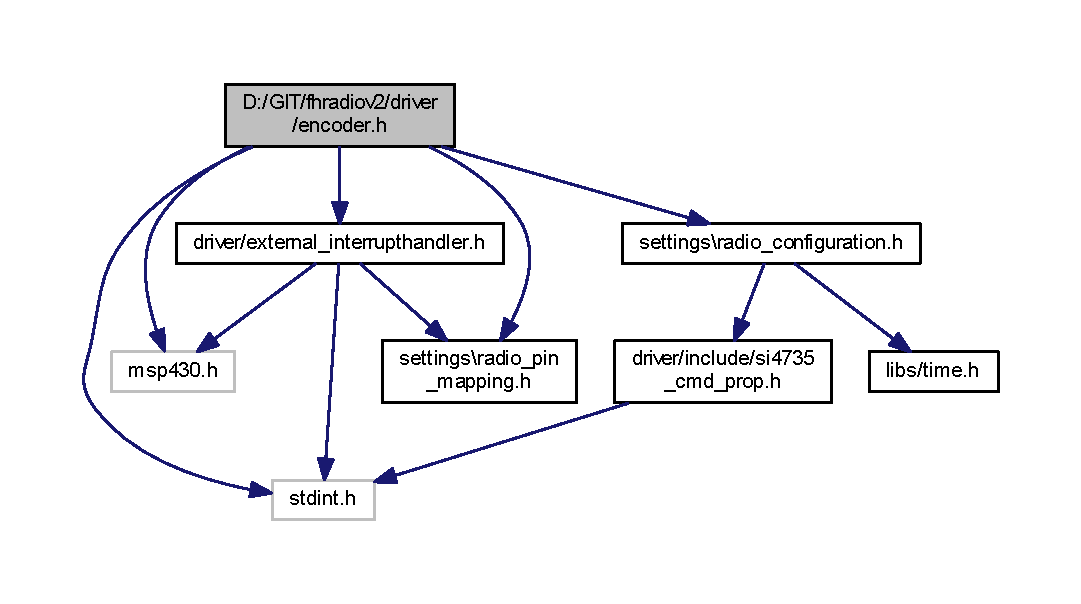
\includegraphics[width=350pt]{encoder_8h__incl}
\end{center}
\end{figure}
Dieser Graph zeigt, welche Datei direkt oder indirekt diese Datei enthält\+:\nopagebreak
\begin{figure}[H]
\begin{center}
\leavevmode
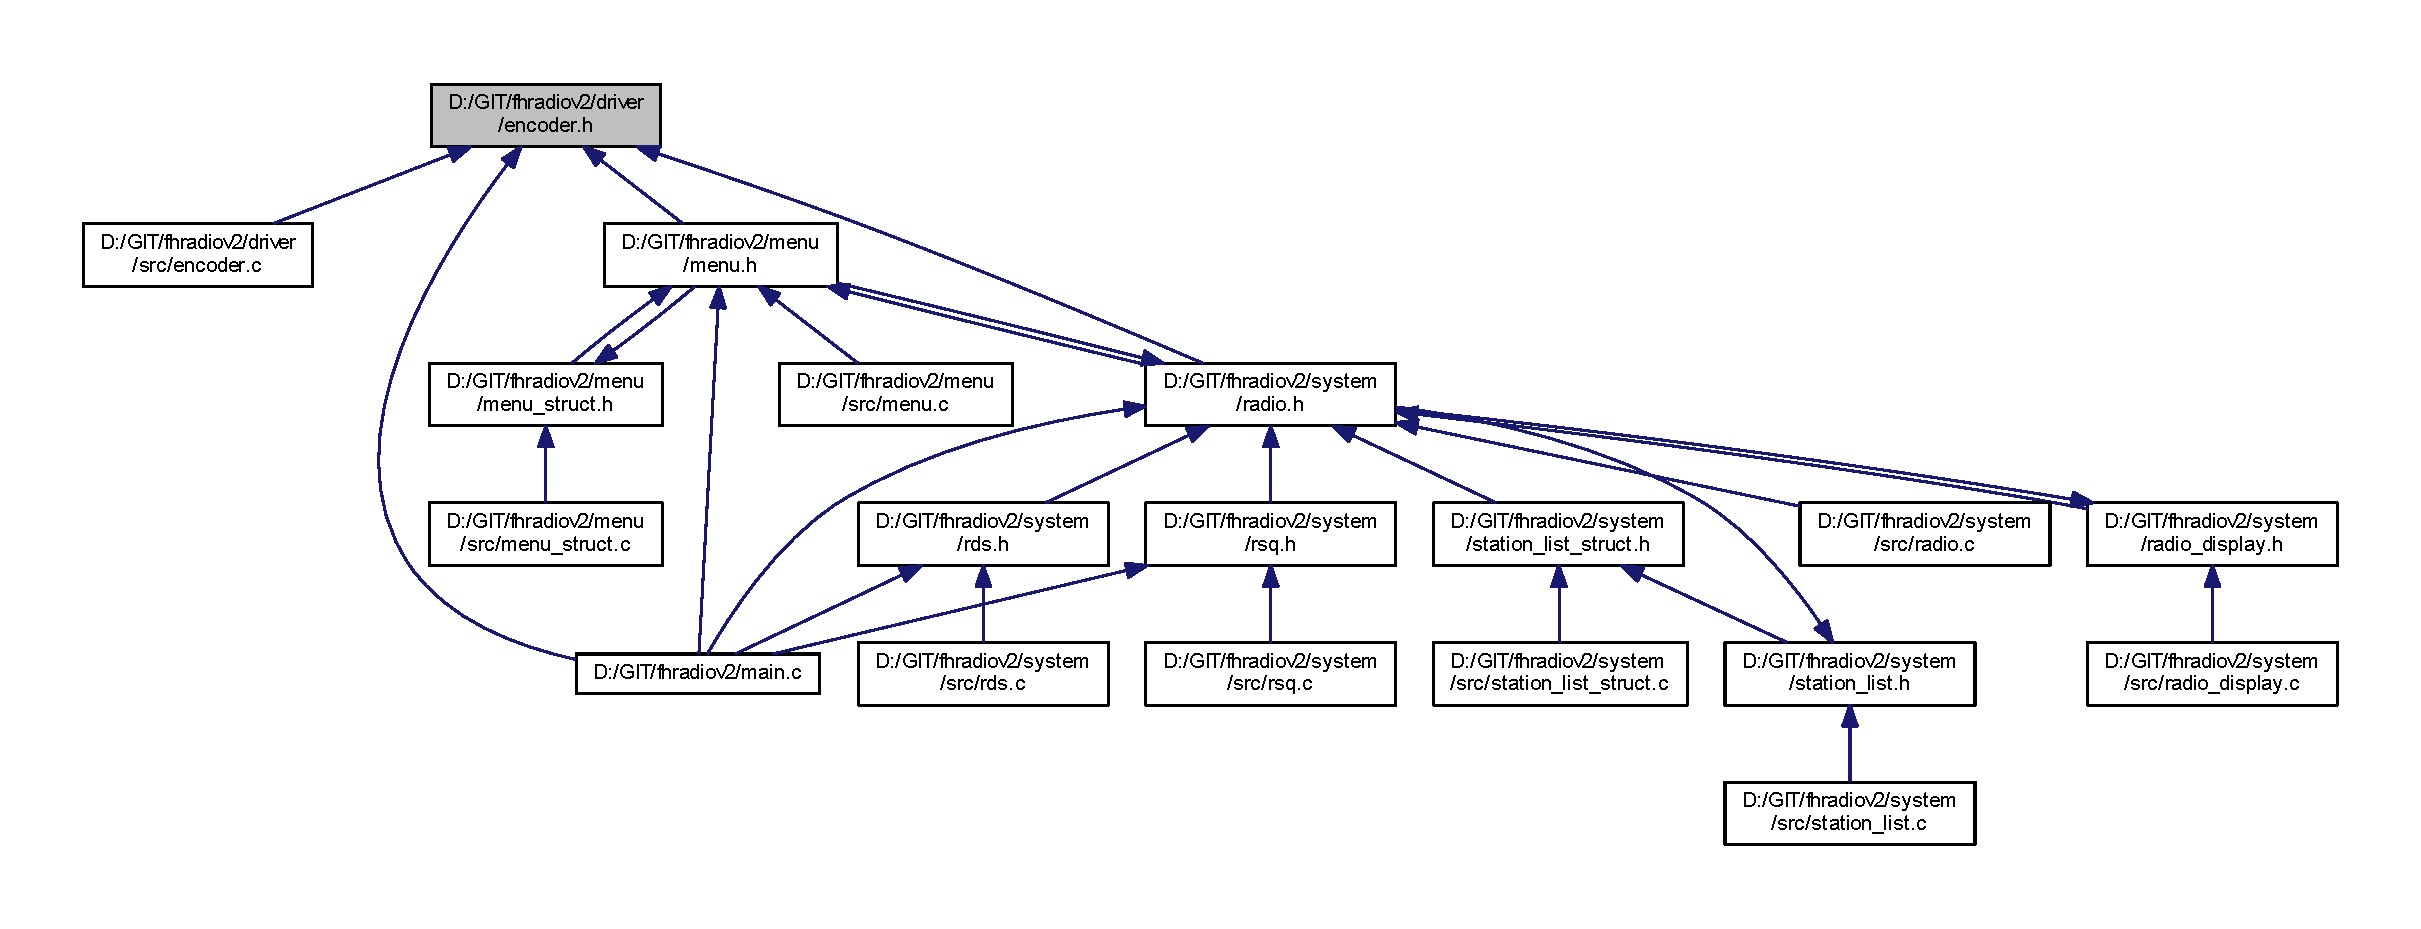
\includegraphics[width=350pt]{encoder_8h__dep__incl}
\end{center}
\end{figure}
\subsection*{Makrodefinitionen}
\begin{DoxyCompactItemize}
\item 
\#define \hyperlink{encoder_8h_a66fa07b195f2bbfb79187fb92fe09d89}{T\+I\+M\+E\+\_\+\+F\+O\+R\+\_\+\+L\+O\+N\+G\+\_\+\+P\+R\+E\+S\+S}~150
\item 
\#define \hyperlink{encoder_8h_afa27376b249650ab2cd2dab80a3aab63}{E\+N\+C\+O\+D\+E\+R\+\_\+1}
\item 
\#define \hyperlink{encoder_8h_a78849ac345e48bff75267b242183df07}{E\+N\+C\+O\+D\+E\+R\+\_\+2}
\item 
\#define \hyperlink{encoder_8h_acb19ebb17d0ed43e47cdd40114f16aa3}{E\+N\+C\+O\+D\+E\+R\+\_\+1\+\_\+\+R\+O\+T\+A\+R\+Y}~0
\item 
\#define \hyperlink{encoder_8h_affaf9d1a3942ffdf7cd97b53b6e888df}{E\+N\+C\+O\+D\+E\+R\+\_\+1\+\_\+\+P\+I\+N}~\hyperlink{radio__pin__mapping_8h_a61b6422841b6c5ab9640866758446063}{E\+N1\+\_\+\+A\+\_\+\+I\+N}
\item 
\#define \hyperlink{encoder_8h_a1e25c308ff36d8efdeb0f27c57313b16}{E\+N\+C\+O\+D\+E\+R\+\_\+1\+\_\+\+D\+I\+R}~\hyperlink{radio__pin__mapping_8h_aeb5004944ba49d984e709a82a4a3a98f}{E\+N1\+\_\+\+A\+\_\+\+D\+I\+R}
\item 
\#define \hyperlink{encoder_8h_aebb67acfd4ffedee07434167e715782a}{E\+N\+C\+O\+D\+E\+R\+\_\+1\+\_\+\+I\+F\+G}~\hyperlink{radio__pin__mapping_8h_a1043fa7116c62a475e5ea1813d23a861}{E\+N1\+\_\+\+A\+\_\+\+I\+F\+G}
\item 
\#define \hyperlink{encoder_8h_a528ca2163adef8b91a9594e72b1827db}{E\+N\+C\+O\+D\+E\+R\+\_\+1\+\_\+\+I\+E\+S}~\hyperlink{radio__pin__mapping_8h_a066c7f99b1e754ff59c882960e093209}{E\+N1\+\_\+\+A\+\_\+\+I\+E\+S}
\item 
\#define \hyperlink{encoder_8h_a9548677fba15c840e8d31ad98c28037c}{E\+N\+C\+O\+D\+E\+R\+\_\+1\+\_\+\+R\+E\+N}~\hyperlink{radio__pin__mapping_8h_ad8bafdfdf1781f3a0919f71c1128c971}{E\+N1\+\_\+\+A\+\_\+\+R\+E\+N}
\item 
\#define \hyperlink{encoder_8h_a9512677f56c7d06024d423529da480c2}{E\+N\+C\+O\+D\+E\+R\+\_\+1\+\_\+\+O\+U\+T}~\hyperlink{radio__pin__mapping_8h_a0b205f6ada4a4c7d68e40950a65c2f85}{E\+N1\+\_\+\+A\+\_\+\+O\+U\+T}
\item 
\#define \hyperlink{encoder_8h_a6545ae719f27ad9aaed9e38fac9c98a6}{E\+N\+C\+O\+D\+E\+R\+\_\+1\+\_\+\+I\+E}~\hyperlink{radio__pin__mapping_8h_a017bdeed62629f89515ecb80f50acd48}{E\+N1\+\_\+\+A\+\_\+\+I\+E}
\item 
\#define \hyperlink{encoder_8h_a476b4d274d2933dd36a689dad7bcf3cd}{E\+N\+C\+O\+D\+E\+R\+\_\+1\+\_\+\+A}~\hyperlink{radio__pin__mapping_8h_a0024d666d429cb9fba37e6643bf0176f}{E\+N1\+\_\+\+A\+\_\+\+P\+I\+N}
\item 
\#define \hyperlink{encoder_8h_acd0e1c9143c5add3894fb1fdb532d417}{E\+N\+C\+O\+D\+E\+R\+\_\+1\+\_\+\+B}~\hyperlink{radio__pin__mapping_8h_ab2f63975ed49814fa8d414fada8921ab}{E\+N1\+\_\+\+B\+\_\+\+P\+I\+N}
\item 
\#define \hyperlink{encoder_8h_a55fc07aa7caa380d293654e23de0ba54}{E\+N\+C\+O\+D\+E\+R\+\_\+1\+\_\+\+T}~\hyperlink{radio__pin__mapping_8h_a54875c0dfa7d0292803b5e36b5da289a}{E\+N1\+\_\+\+T\+A\+S\+T\+\_\+\+P\+I\+N}
\item 
\#define \hyperlink{encoder_8h_acb19ebb17d0ed43e47cdd40114f16aa3}{E\+N\+C\+O\+D\+E\+R\+\_\+1\+\_\+\+R\+O\+T\+A\+R\+Y}~0
\item 
\#define \hyperlink{encoder_8h_afefc9c30fe7e9e3151dddc3a1516fee6}{E\+N\+C\+O\+D\+E\+R\+\_\+2\+\_\+\+P\+I\+N}~P2\+I\+N
\item 
\#define \hyperlink{encoder_8h_ac24b20e625098815fab972b6e7ac382b}{E\+N\+C\+O\+D\+E\+R\+\_\+2\+\_\+\+D\+I\+R}~P2\+D\+I\+R
\item 
\#define \hyperlink{encoder_8h_ac52f7da62f5e616c23b69b1551d8df26}{E\+N\+C\+O\+D\+E\+R\+\_\+2\+\_\+\+I\+F\+G}~P2\+I\+F\+G
\item 
\#define \hyperlink{encoder_8h_af65e203e8221f10df3841caee401a659}{E\+N\+C\+O\+D\+E\+R\+\_\+2\+\_\+\+I\+E\+S}~P2\+I\+E\+S
\item 
\#define \hyperlink{encoder_8h_aa3ad3b0b79178fe00bcbac4fc278c2b2}{E\+N\+C\+O\+D\+E\+R\+\_\+2\+\_\+\+R\+E\+N}~P2\+R\+E\+N
\item 
\#define \hyperlink{encoder_8h_ad029c73a3e4d1fed315c2d1c521a197e}{E\+N\+C\+O\+D\+E\+R\+\_\+2\+\_\+\+O\+U\+T}~P2\+O\+U\+T
\item 
\#define \hyperlink{encoder_8h_a64db25a3ea079732b5349232440d065e}{E\+N\+C\+O\+D\+E\+R\+\_\+2\+\_\+\+I\+E}~P2\+I\+E
\item 
\#define \hyperlink{encoder_8h_a2782b5e9a4cf798d655b641ff929525b}{E\+N\+C\+O\+D\+E\+R\+\_\+2\+\_\+\+A}~B\+I\+T0
\item 
\#define \hyperlink{encoder_8h_aeb5875573ea25c506967e4023638da24}{E\+N\+C\+O\+D\+E\+R\+\_\+2\+\_\+\+B}~B\+I\+T1
\item 
\#define \hyperlink{encoder_8h_aa31b57ce8a73b2d9c6db28ebe93ab40b}{E\+N\+C\+O\+D\+E\+R\+\_\+2\+\_\+\+T}~B\+I\+T2
\end{DoxyCompactItemize}
\subsection*{Funktionen}
\begin{DoxyCompactItemize}
\item 
void \hyperlink{encoder_8h_af5a0c9bea9a0da18fa1c123af8f2877c}{Encoder\+\_\+\+Timer\+\_\+init} (void)
\item 
void \hyperlink{encoder_8h_a271ca5c0624ed124f6398f408d1f3017}{encoder\+\_\+interrupt} (void)
\item 
void \hyperlink{encoder_8h_a136248fd00f8429933544a54b030aef9}{encoder\+\_\+interrupt2} (void)
\item 
void \hyperlink{encoder_8h_a1b09f480da15d565de0b4acf37f40199}{Encoder\+\_\+1\+\_\+init} (void)
\item 
void \hyperlink{encoder_8h_afcb65d25ec031240b72ae3a51c1e9b4a}{Encoder\+\_\+1\+\_\+decoder} (void)
\item 
int16\+\_\+t \hyperlink{encoder_8h_a7a39090bb6f1d88f9371e44f4923194b}{Encoder\+\_\+1\+\_\+get\+\_\+count} ()
\item 
void \hyperlink{encoder_8h_af947b4bf6e9bc6d5b580609d046789da}{Encoder\+\_\+2\+\_\+init} (void)
\item 
void \hyperlink{encoder_8h_a81332b0a52a42a7a7b134228f9bb3848}{Encoder\+\_\+2\+\_\+decoder} (void)
\item 
int16\+\_\+t \hyperlink{encoder_8h_a17708354c0e76c0422398f8dcd50dfea}{Encoder\+\_\+2\+\_\+get\+\_\+count} ()
\end{DoxyCompactItemize}


\subsection{Makro-\/\+Dokumentation}
\hypertarget{encoder_8h_afa27376b249650ab2cd2dab80a3aab63}{}\index{encoder.\+h@{encoder.\+h}!E\+N\+C\+O\+D\+E\+R\+\_\+1@{E\+N\+C\+O\+D\+E\+R\+\_\+1}}
\index{E\+N\+C\+O\+D\+E\+R\+\_\+1@{E\+N\+C\+O\+D\+E\+R\+\_\+1}!encoder.\+h@{encoder.\+h}}
\subsubsection[{E\+N\+C\+O\+D\+E\+R\+\_\+1}]{\setlength{\rightskip}{0pt plus 5cm}\#define E\+N\+C\+O\+D\+E\+R\+\_\+1}\label{encoder_8h_afa27376b249650ab2cd2dab80a3aab63}


Definiert in Zeile 19 der Datei encoder.\+h.

\hypertarget{encoder_8h_a476b4d274d2933dd36a689dad7bcf3cd}{}\index{encoder.\+h@{encoder.\+h}!E\+N\+C\+O\+D\+E\+R\+\_\+1\+\_\+\+A@{E\+N\+C\+O\+D\+E\+R\+\_\+1\+\_\+\+A}}
\index{E\+N\+C\+O\+D\+E\+R\+\_\+1\+\_\+\+A@{E\+N\+C\+O\+D\+E\+R\+\_\+1\+\_\+\+A}!encoder.\+h@{encoder.\+h}}
\subsubsection[{E\+N\+C\+O\+D\+E\+R\+\_\+1\+\_\+\+A}]{\setlength{\rightskip}{0pt plus 5cm}\#define E\+N\+C\+O\+D\+E\+R\+\_\+1\+\_\+\+A~{\bf E\+N1\+\_\+\+A\+\_\+\+P\+I\+N}}\label{encoder_8h_a476b4d274d2933dd36a689dad7bcf3cd}


Definiert in Zeile 35 der Datei encoder.\+h.

\hypertarget{encoder_8h_acd0e1c9143c5add3894fb1fdb532d417}{}\index{encoder.\+h@{encoder.\+h}!E\+N\+C\+O\+D\+E\+R\+\_\+1\+\_\+\+B@{E\+N\+C\+O\+D\+E\+R\+\_\+1\+\_\+\+B}}
\index{E\+N\+C\+O\+D\+E\+R\+\_\+1\+\_\+\+B@{E\+N\+C\+O\+D\+E\+R\+\_\+1\+\_\+\+B}!encoder.\+h@{encoder.\+h}}
\subsubsection[{E\+N\+C\+O\+D\+E\+R\+\_\+1\+\_\+\+B}]{\setlength{\rightskip}{0pt plus 5cm}\#define E\+N\+C\+O\+D\+E\+R\+\_\+1\+\_\+\+B~{\bf E\+N1\+\_\+\+B\+\_\+\+P\+I\+N}}\label{encoder_8h_acd0e1c9143c5add3894fb1fdb532d417}


Definiert in Zeile 36 der Datei encoder.\+h.

\hypertarget{encoder_8h_a1e25c308ff36d8efdeb0f27c57313b16}{}\index{encoder.\+h@{encoder.\+h}!E\+N\+C\+O\+D\+E\+R\+\_\+1\+\_\+\+D\+I\+R@{E\+N\+C\+O\+D\+E\+R\+\_\+1\+\_\+\+D\+I\+R}}
\index{E\+N\+C\+O\+D\+E\+R\+\_\+1\+\_\+\+D\+I\+R@{E\+N\+C\+O\+D\+E\+R\+\_\+1\+\_\+\+D\+I\+R}!encoder.\+h@{encoder.\+h}}
\subsubsection[{E\+N\+C\+O\+D\+E\+R\+\_\+1\+\_\+\+D\+I\+R}]{\setlength{\rightskip}{0pt plus 5cm}\#define E\+N\+C\+O\+D\+E\+R\+\_\+1\+\_\+\+D\+I\+R~{\bf E\+N1\+\_\+\+A\+\_\+\+D\+I\+R}}\label{encoder_8h_a1e25c308ff36d8efdeb0f27c57313b16}


Definiert in Zeile 29 der Datei encoder.\+h.

\hypertarget{encoder_8h_a6545ae719f27ad9aaed9e38fac9c98a6}{}\index{encoder.\+h@{encoder.\+h}!E\+N\+C\+O\+D\+E\+R\+\_\+1\+\_\+\+I\+E@{E\+N\+C\+O\+D\+E\+R\+\_\+1\+\_\+\+I\+E}}
\index{E\+N\+C\+O\+D\+E\+R\+\_\+1\+\_\+\+I\+E@{E\+N\+C\+O\+D\+E\+R\+\_\+1\+\_\+\+I\+E}!encoder.\+h@{encoder.\+h}}
\subsubsection[{E\+N\+C\+O\+D\+E\+R\+\_\+1\+\_\+\+I\+E}]{\setlength{\rightskip}{0pt plus 5cm}\#define E\+N\+C\+O\+D\+E\+R\+\_\+1\+\_\+\+I\+E~{\bf E\+N1\+\_\+\+A\+\_\+\+I\+E}}\label{encoder_8h_a6545ae719f27ad9aaed9e38fac9c98a6}


Definiert in Zeile 34 der Datei encoder.\+h.

\hypertarget{encoder_8h_a528ca2163adef8b91a9594e72b1827db}{}\index{encoder.\+h@{encoder.\+h}!E\+N\+C\+O\+D\+E\+R\+\_\+1\+\_\+\+I\+E\+S@{E\+N\+C\+O\+D\+E\+R\+\_\+1\+\_\+\+I\+E\+S}}
\index{E\+N\+C\+O\+D\+E\+R\+\_\+1\+\_\+\+I\+E\+S@{E\+N\+C\+O\+D\+E\+R\+\_\+1\+\_\+\+I\+E\+S}!encoder.\+h@{encoder.\+h}}
\subsubsection[{E\+N\+C\+O\+D\+E\+R\+\_\+1\+\_\+\+I\+E\+S}]{\setlength{\rightskip}{0pt plus 5cm}\#define E\+N\+C\+O\+D\+E\+R\+\_\+1\+\_\+\+I\+E\+S~{\bf E\+N1\+\_\+\+A\+\_\+\+I\+E\+S}}\label{encoder_8h_a528ca2163adef8b91a9594e72b1827db}


Definiert in Zeile 31 der Datei encoder.\+h.

\hypertarget{encoder_8h_aebb67acfd4ffedee07434167e715782a}{}\index{encoder.\+h@{encoder.\+h}!E\+N\+C\+O\+D\+E\+R\+\_\+1\+\_\+\+I\+F\+G@{E\+N\+C\+O\+D\+E\+R\+\_\+1\+\_\+\+I\+F\+G}}
\index{E\+N\+C\+O\+D\+E\+R\+\_\+1\+\_\+\+I\+F\+G@{E\+N\+C\+O\+D\+E\+R\+\_\+1\+\_\+\+I\+F\+G}!encoder.\+h@{encoder.\+h}}
\subsubsection[{E\+N\+C\+O\+D\+E\+R\+\_\+1\+\_\+\+I\+F\+G}]{\setlength{\rightskip}{0pt plus 5cm}\#define E\+N\+C\+O\+D\+E\+R\+\_\+1\+\_\+\+I\+F\+G~{\bf E\+N1\+\_\+\+A\+\_\+\+I\+F\+G}}\label{encoder_8h_aebb67acfd4ffedee07434167e715782a}


Definiert in Zeile 30 der Datei encoder.\+h.

\hypertarget{encoder_8h_a9512677f56c7d06024d423529da480c2}{}\index{encoder.\+h@{encoder.\+h}!E\+N\+C\+O\+D\+E\+R\+\_\+1\+\_\+\+O\+U\+T@{E\+N\+C\+O\+D\+E\+R\+\_\+1\+\_\+\+O\+U\+T}}
\index{E\+N\+C\+O\+D\+E\+R\+\_\+1\+\_\+\+O\+U\+T@{E\+N\+C\+O\+D\+E\+R\+\_\+1\+\_\+\+O\+U\+T}!encoder.\+h@{encoder.\+h}}
\subsubsection[{E\+N\+C\+O\+D\+E\+R\+\_\+1\+\_\+\+O\+U\+T}]{\setlength{\rightskip}{0pt plus 5cm}\#define E\+N\+C\+O\+D\+E\+R\+\_\+1\+\_\+\+O\+U\+T~{\bf E\+N1\+\_\+\+A\+\_\+\+O\+U\+T}}\label{encoder_8h_a9512677f56c7d06024d423529da480c2}


Definiert in Zeile 33 der Datei encoder.\+h.

\hypertarget{encoder_8h_affaf9d1a3942ffdf7cd97b53b6e888df}{}\index{encoder.\+h@{encoder.\+h}!E\+N\+C\+O\+D\+E\+R\+\_\+1\+\_\+\+P\+I\+N@{E\+N\+C\+O\+D\+E\+R\+\_\+1\+\_\+\+P\+I\+N}}
\index{E\+N\+C\+O\+D\+E\+R\+\_\+1\+\_\+\+P\+I\+N@{E\+N\+C\+O\+D\+E\+R\+\_\+1\+\_\+\+P\+I\+N}!encoder.\+h@{encoder.\+h}}
\subsubsection[{E\+N\+C\+O\+D\+E\+R\+\_\+1\+\_\+\+P\+I\+N}]{\setlength{\rightskip}{0pt plus 5cm}\#define E\+N\+C\+O\+D\+E\+R\+\_\+1\+\_\+\+P\+I\+N~{\bf E\+N1\+\_\+\+A\+\_\+\+I\+N}}\label{encoder_8h_affaf9d1a3942ffdf7cd97b53b6e888df}


Definiert in Zeile 28 der Datei encoder.\+h.

\hypertarget{encoder_8h_a9548677fba15c840e8d31ad98c28037c}{}\index{encoder.\+h@{encoder.\+h}!E\+N\+C\+O\+D\+E\+R\+\_\+1\+\_\+\+R\+E\+N@{E\+N\+C\+O\+D\+E\+R\+\_\+1\+\_\+\+R\+E\+N}}
\index{E\+N\+C\+O\+D\+E\+R\+\_\+1\+\_\+\+R\+E\+N@{E\+N\+C\+O\+D\+E\+R\+\_\+1\+\_\+\+R\+E\+N}!encoder.\+h@{encoder.\+h}}
\subsubsection[{E\+N\+C\+O\+D\+E\+R\+\_\+1\+\_\+\+R\+E\+N}]{\setlength{\rightskip}{0pt plus 5cm}\#define E\+N\+C\+O\+D\+E\+R\+\_\+1\+\_\+\+R\+E\+N~{\bf E\+N1\+\_\+\+A\+\_\+\+R\+E\+N}}\label{encoder_8h_a9548677fba15c840e8d31ad98c28037c}


Definiert in Zeile 32 der Datei encoder.\+h.

\hypertarget{encoder_8h_acb19ebb17d0ed43e47cdd40114f16aa3}{}\index{encoder.\+h@{encoder.\+h}!E\+N\+C\+O\+D\+E\+R\+\_\+1\+\_\+\+R\+O\+T\+A\+R\+Y@{E\+N\+C\+O\+D\+E\+R\+\_\+1\+\_\+\+R\+O\+T\+A\+R\+Y}}
\index{E\+N\+C\+O\+D\+E\+R\+\_\+1\+\_\+\+R\+O\+T\+A\+R\+Y@{E\+N\+C\+O\+D\+E\+R\+\_\+1\+\_\+\+R\+O\+T\+A\+R\+Y}!encoder.\+h@{encoder.\+h}}
\subsubsection[{E\+N\+C\+O\+D\+E\+R\+\_\+1\+\_\+\+R\+O\+T\+A\+R\+Y}]{\setlength{\rightskip}{0pt plus 5cm}\#define E\+N\+C\+O\+D\+E\+R\+\_\+1\+\_\+\+R\+O\+T\+A\+R\+Y~0}\label{encoder_8h_acb19ebb17d0ed43e47cdd40114f16aa3}


Definiert in Zeile 48 der Datei encoder.\+h.

\hypertarget{encoder_8h_acb19ebb17d0ed43e47cdd40114f16aa3}{}\index{encoder.\+h@{encoder.\+h}!E\+N\+C\+O\+D\+E\+R\+\_\+1\+\_\+\+R\+O\+T\+A\+R\+Y@{E\+N\+C\+O\+D\+E\+R\+\_\+1\+\_\+\+R\+O\+T\+A\+R\+Y}}
\index{E\+N\+C\+O\+D\+E\+R\+\_\+1\+\_\+\+R\+O\+T\+A\+R\+Y@{E\+N\+C\+O\+D\+E\+R\+\_\+1\+\_\+\+R\+O\+T\+A\+R\+Y}!encoder.\+h@{encoder.\+h}}
\subsubsection[{E\+N\+C\+O\+D\+E\+R\+\_\+1\+\_\+\+R\+O\+T\+A\+R\+Y}]{\setlength{\rightskip}{0pt plus 5cm}\#define E\+N\+C\+O\+D\+E\+R\+\_\+1\+\_\+\+R\+O\+T\+A\+R\+Y~0}\label{encoder_8h_acb19ebb17d0ed43e47cdd40114f16aa3}


Definiert in Zeile 48 der Datei encoder.\+h.

\hypertarget{encoder_8h_a55fc07aa7caa380d293654e23de0ba54}{}\index{encoder.\+h@{encoder.\+h}!E\+N\+C\+O\+D\+E\+R\+\_\+1\+\_\+\+T@{E\+N\+C\+O\+D\+E\+R\+\_\+1\+\_\+\+T}}
\index{E\+N\+C\+O\+D\+E\+R\+\_\+1\+\_\+\+T@{E\+N\+C\+O\+D\+E\+R\+\_\+1\+\_\+\+T}!encoder.\+h@{encoder.\+h}}
\subsubsection[{E\+N\+C\+O\+D\+E\+R\+\_\+1\+\_\+\+T}]{\setlength{\rightskip}{0pt plus 5cm}\#define E\+N\+C\+O\+D\+E\+R\+\_\+1\+\_\+\+T~{\bf E\+N1\+\_\+\+T\+A\+S\+T\+\_\+\+P\+I\+N}}\label{encoder_8h_a55fc07aa7caa380d293654e23de0ba54}


Definiert in Zeile 37 der Datei encoder.\+h.

\hypertarget{encoder_8h_a78849ac345e48bff75267b242183df07}{}\index{encoder.\+h@{encoder.\+h}!E\+N\+C\+O\+D\+E\+R\+\_\+2@{E\+N\+C\+O\+D\+E\+R\+\_\+2}}
\index{E\+N\+C\+O\+D\+E\+R\+\_\+2@{E\+N\+C\+O\+D\+E\+R\+\_\+2}!encoder.\+h@{encoder.\+h}}
\subsubsection[{E\+N\+C\+O\+D\+E\+R\+\_\+2}]{\setlength{\rightskip}{0pt plus 5cm}\#define E\+N\+C\+O\+D\+E\+R\+\_\+2}\label{encoder_8h_a78849ac345e48bff75267b242183df07}


Definiert in Zeile 20 der Datei encoder.\+h.

\hypertarget{encoder_8h_a2782b5e9a4cf798d655b641ff929525b}{}\index{encoder.\+h@{encoder.\+h}!E\+N\+C\+O\+D\+E\+R\+\_\+2\+\_\+\+A@{E\+N\+C\+O\+D\+E\+R\+\_\+2\+\_\+\+A}}
\index{E\+N\+C\+O\+D\+E\+R\+\_\+2\+\_\+\+A@{E\+N\+C\+O\+D\+E\+R\+\_\+2\+\_\+\+A}!encoder.\+h@{encoder.\+h}}
\subsubsection[{E\+N\+C\+O\+D\+E\+R\+\_\+2\+\_\+\+A}]{\setlength{\rightskip}{0pt plus 5cm}\#define E\+N\+C\+O\+D\+E\+R\+\_\+2\+\_\+\+A~B\+I\+T0}\label{encoder_8h_a2782b5e9a4cf798d655b641ff929525b}


Definiert in Zeile 56 der Datei encoder.\+h.

\hypertarget{encoder_8h_aeb5875573ea25c506967e4023638da24}{}\index{encoder.\+h@{encoder.\+h}!E\+N\+C\+O\+D\+E\+R\+\_\+2\+\_\+\+B@{E\+N\+C\+O\+D\+E\+R\+\_\+2\+\_\+\+B}}
\index{E\+N\+C\+O\+D\+E\+R\+\_\+2\+\_\+\+B@{E\+N\+C\+O\+D\+E\+R\+\_\+2\+\_\+\+B}!encoder.\+h@{encoder.\+h}}
\subsubsection[{E\+N\+C\+O\+D\+E\+R\+\_\+2\+\_\+\+B}]{\setlength{\rightskip}{0pt plus 5cm}\#define E\+N\+C\+O\+D\+E\+R\+\_\+2\+\_\+\+B~B\+I\+T1}\label{encoder_8h_aeb5875573ea25c506967e4023638da24}


Definiert in Zeile 57 der Datei encoder.\+h.

\hypertarget{encoder_8h_ac24b20e625098815fab972b6e7ac382b}{}\index{encoder.\+h@{encoder.\+h}!E\+N\+C\+O\+D\+E\+R\+\_\+2\+\_\+\+D\+I\+R@{E\+N\+C\+O\+D\+E\+R\+\_\+2\+\_\+\+D\+I\+R}}
\index{E\+N\+C\+O\+D\+E\+R\+\_\+2\+\_\+\+D\+I\+R@{E\+N\+C\+O\+D\+E\+R\+\_\+2\+\_\+\+D\+I\+R}!encoder.\+h@{encoder.\+h}}
\subsubsection[{E\+N\+C\+O\+D\+E\+R\+\_\+2\+\_\+\+D\+I\+R}]{\setlength{\rightskip}{0pt plus 5cm}\#define E\+N\+C\+O\+D\+E\+R\+\_\+2\+\_\+\+D\+I\+R~P2\+D\+I\+R}\label{encoder_8h_ac24b20e625098815fab972b6e7ac382b}


Definiert in Zeile 50 der Datei encoder.\+h.

\hypertarget{encoder_8h_a64db25a3ea079732b5349232440d065e}{}\index{encoder.\+h@{encoder.\+h}!E\+N\+C\+O\+D\+E\+R\+\_\+2\+\_\+\+I\+E@{E\+N\+C\+O\+D\+E\+R\+\_\+2\+\_\+\+I\+E}}
\index{E\+N\+C\+O\+D\+E\+R\+\_\+2\+\_\+\+I\+E@{E\+N\+C\+O\+D\+E\+R\+\_\+2\+\_\+\+I\+E}!encoder.\+h@{encoder.\+h}}
\subsubsection[{E\+N\+C\+O\+D\+E\+R\+\_\+2\+\_\+\+I\+E}]{\setlength{\rightskip}{0pt plus 5cm}\#define E\+N\+C\+O\+D\+E\+R\+\_\+2\+\_\+\+I\+E~P2\+I\+E}\label{encoder_8h_a64db25a3ea079732b5349232440d065e}


Definiert in Zeile 55 der Datei encoder.\+h.

\hypertarget{encoder_8h_af65e203e8221f10df3841caee401a659}{}\index{encoder.\+h@{encoder.\+h}!E\+N\+C\+O\+D\+E\+R\+\_\+2\+\_\+\+I\+E\+S@{E\+N\+C\+O\+D\+E\+R\+\_\+2\+\_\+\+I\+E\+S}}
\index{E\+N\+C\+O\+D\+E\+R\+\_\+2\+\_\+\+I\+E\+S@{E\+N\+C\+O\+D\+E\+R\+\_\+2\+\_\+\+I\+E\+S}!encoder.\+h@{encoder.\+h}}
\subsubsection[{E\+N\+C\+O\+D\+E\+R\+\_\+2\+\_\+\+I\+E\+S}]{\setlength{\rightskip}{0pt plus 5cm}\#define E\+N\+C\+O\+D\+E\+R\+\_\+2\+\_\+\+I\+E\+S~P2\+I\+E\+S}\label{encoder_8h_af65e203e8221f10df3841caee401a659}


Definiert in Zeile 52 der Datei encoder.\+h.

\hypertarget{encoder_8h_ac52f7da62f5e616c23b69b1551d8df26}{}\index{encoder.\+h@{encoder.\+h}!E\+N\+C\+O\+D\+E\+R\+\_\+2\+\_\+\+I\+F\+G@{E\+N\+C\+O\+D\+E\+R\+\_\+2\+\_\+\+I\+F\+G}}
\index{E\+N\+C\+O\+D\+E\+R\+\_\+2\+\_\+\+I\+F\+G@{E\+N\+C\+O\+D\+E\+R\+\_\+2\+\_\+\+I\+F\+G}!encoder.\+h@{encoder.\+h}}
\subsubsection[{E\+N\+C\+O\+D\+E\+R\+\_\+2\+\_\+\+I\+F\+G}]{\setlength{\rightskip}{0pt plus 5cm}\#define E\+N\+C\+O\+D\+E\+R\+\_\+2\+\_\+\+I\+F\+G~P2\+I\+F\+G}\label{encoder_8h_ac52f7da62f5e616c23b69b1551d8df26}


Definiert in Zeile 51 der Datei encoder.\+h.

\hypertarget{encoder_8h_ad029c73a3e4d1fed315c2d1c521a197e}{}\index{encoder.\+h@{encoder.\+h}!E\+N\+C\+O\+D\+E\+R\+\_\+2\+\_\+\+O\+U\+T@{E\+N\+C\+O\+D\+E\+R\+\_\+2\+\_\+\+O\+U\+T}}
\index{E\+N\+C\+O\+D\+E\+R\+\_\+2\+\_\+\+O\+U\+T@{E\+N\+C\+O\+D\+E\+R\+\_\+2\+\_\+\+O\+U\+T}!encoder.\+h@{encoder.\+h}}
\subsubsection[{E\+N\+C\+O\+D\+E\+R\+\_\+2\+\_\+\+O\+U\+T}]{\setlength{\rightskip}{0pt plus 5cm}\#define E\+N\+C\+O\+D\+E\+R\+\_\+2\+\_\+\+O\+U\+T~P2\+O\+U\+T}\label{encoder_8h_ad029c73a3e4d1fed315c2d1c521a197e}


Definiert in Zeile 54 der Datei encoder.\+h.

\hypertarget{encoder_8h_afefc9c30fe7e9e3151dddc3a1516fee6}{}\index{encoder.\+h@{encoder.\+h}!E\+N\+C\+O\+D\+E\+R\+\_\+2\+\_\+\+P\+I\+N@{E\+N\+C\+O\+D\+E\+R\+\_\+2\+\_\+\+P\+I\+N}}
\index{E\+N\+C\+O\+D\+E\+R\+\_\+2\+\_\+\+P\+I\+N@{E\+N\+C\+O\+D\+E\+R\+\_\+2\+\_\+\+P\+I\+N}!encoder.\+h@{encoder.\+h}}
\subsubsection[{E\+N\+C\+O\+D\+E\+R\+\_\+2\+\_\+\+P\+I\+N}]{\setlength{\rightskip}{0pt plus 5cm}\#define E\+N\+C\+O\+D\+E\+R\+\_\+2\+\_\+\+P\+I\+N~P2\+I\+N}\label{encoder_8h_afefc9c30fe7e9e3151dddc3a1516fee6}


Definiert in Zeile 49 der Datei encoder.\+h.

\hypertarget{encoder_8h_aa3ad3b0b79178fe00bcbac4fc278c2b2}{}\index{encoder.\+h@{encoder.\+h}!E\+N\+C\+O\+D\+E\+R\+\_\+2\+\_\+\+R\+E\+N@{E\+N\+C\+O\+D\+E\+R\+\_\+2\+\_\+\+R\+E\+N}}
\index{E\+N\+C\+O\+D\+E\+R\+\_\+2\+\_\+\+R\+E\+N@{E\+N\+C\+O\+D\+E\+R\+\_\+2\+\_\+\+R\+E\+N}!encoder.\+h@{encoder.\+h}}
\subsubsection[{E\+N\+C\+O\+D\+E\+R\+\_\+2\+\_\+\+R\+E\+N}]{\setlength{\rightskip}{0pt plus 5cm}\#define E\+N\+C\+O\+D\+E\+R\+\_\+2\+\_\+\+R\+E\+N~P2\+R\+E\+N}\label{encoder_8h_aa3ad3b0b79178fe00bcbac4fc278c2b2}


Definiert in Zeile 53 der Datei encoder.\+h.

\hypertarget{encoder_8h_aa31b57ce8a73b2d9c6db28ebe93ab40b}{}\index{encoder.\+h@{encoder.\+h}!E\+N\+C\+O\+D\+E\+R\+\_\+2\+\_\+\+T@{E\+N\+C\+O\+D\+E\+R\+\_\+2\+\_\+\+T}}
\index{E\+N\+C\+O\+D\+E\+R\+\_\+2\+\_\+\+T@{E\+N\+C\+O\+D\+E\+R\+\_\+2\+\_\+\+T}!encoder.\+h@{encoder.\+h}}
\subsubsection[{E\+N\+C\+O\+D\+E\+R\+\_\+2\+\_\+\+T}]{\setlength{\rightskip}{0pt plus 5cm}\#define E\+N\+C\+O\+D\+E\+R\+\_\+2\+\_\+\+T~B\+I\+T2}\label{encoder_8h_aa31b57ce8a73b2d9c6db28ebe93ab40b}


Definiert in Zeile 58 der Datei encoder.\+h.

\hypertarget{encoder_8h_a66fa07b195f2bbfb79187fb92fe09d89}{}\index{encoder.\+h@{encoder.\+h}!T\+I\+M\+E\+\_\+\+F\+O\+R\+\_\+\+L\+O\+N\+G\+\_\+\+P\+R\+E\+S\+S@{T\+I\+M\+E\+\_\+\+F\+O\+R\+\_\+\+L\+O\+N\+G\+\_\+\+P\+R\+E\+S\+S}}
\index{T\+I\+M\+E\+\_\+\+F\+O\+R\+\_\+\+L\+O\+N\+G\+\_\+\+P\+R\+E\+S\+S@{T\+I\+M\+E\+\_\+\+F\+O\+R\+\_\+\+L\+O\+N\+G\+\_\+\+P\+R\+E\+S\+S}!encoder.\+h@{encoder.\+h}}
\subsubsection[{T\+I\+M\+E\+\_\+\+F\+O\+R\+\_\+\+L\+O\+N\+G\+\_\+\+P\+R\+E\+S\+S}]{\setlength{\rightskip}{0pt plus 5cm}\#define T\+I\+M\+E\+\_\+\+F\+O\+R\+\_\+\+L\+O\+N\+G\+\_\+\+P\+R\+E\+S\+S~150}\label{encoder_8h_a66fa07b195f2bbfb79187fb92fe09d89}


Definiert in Zeile 17 der Datei encoder.\+h.



\subsection{Dokumentation der Funktionen}
\hypertarget{encoder_8h_afcb65d25ec031240b72ae3a51c1e9b4a}{}\index{encoder.\+h@{encoder.\+h}!Encoder\+\_\+1\+\_\+decoder@{Encoder\+\_\+1\+\_\+decoder}}
\index{Encoder\+\_\+1\+\_\+decoder@{Encoder\+\_\+1\+\_\+decoder}!encoder.\+h@{encoder.\+h}}
\subsubsection[{Encoder\+\_\+1\+\_\+decoder}]{\setlength{\rightskip}{0pt plus 5cm}void Encoder\+\_\+1\+\_\+decoder (
\begin{DoxyParamCaption}
\item[{void}]{}
\end{DoxyParamCaption}
)}\label{encoder_8h_afcb65d25ec031240b72ae3a51c1e9b4a}
\hypertarget{encoder_8h_a7a39090bb6f1d88f9371e44f4923194b}{}\index{encoder.\+h@{encoder.\+h}!Encoder\+\_\+1\+\_\+get\+\_\+count@{Encoder\+\_\+1\+\_\+get\+\_\+count}}
\index{Encoder\+\_\+1\+\_\+get\+\_\+count@{Encoder\+\_\+1\+\_\+get\+\_\+count}!encoder.\+h@{encoder.\+h}}
\subsubsection[{Encoder\+\_\+1\+\_\+get\+\_\+count}]{\setlength{\rightskip}{0pt plus 5cm}int16\+\_\+t Encoder\+\_\+1\+\_\+get\+\_\+count (
\begin{DoxyParamCaption}
{}
\end{DoxyParamCaption}
)}\label{encoder_8h_a7a39090bb6f1d88f9371e44f4923194b}


Hier ist ein Graph der zeigt, wo diese Funktion aufgerufen wird\+:\nopagebreak
\begin{figure}[H]
\begin{center}
\leavevmode
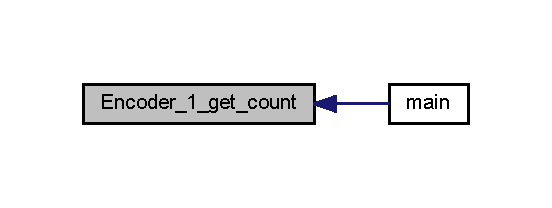
\includegraphics[width=265pt]{encoder_8h_a7a39090bb6f1d88f9371e44f4923194b_icgraph}
\end{center}
\end{figure}


\hypertarget{encoder_8h_a1b09f480da15d565de0b4acf37f40199}{}\index{encoder.\+h@{encoder.\+h}!Encoder\+\_\+1\+\_\+init@{Encoder\+\_\+1\+\_\+init}}
\index{Encoder\+\_\+1\+\_\+init@{Encoder\+\_\+1\+\_\+init}!encoder.\+h@{encoder.\+h}}
\subsubsection[{Encoder\+\_\+1\+\_\+init}]{\setlength{\rightskip}{0pt plus 5cm}void Encoder\+\_\+1\+\_\+init (
\begin{DoxyParamCaption}
\item[{void}]{}
\end{DoxyParamCaption}
)}\label{encoder_8h_a1b09f480da15d565de0b4acf37f40199}


Hier ist ein Graph der zeigt, wo diese Funktion aufgerufen wird\+:\nopagebreak
\begin{figure}[H]
\begin{center}
\leavevmode
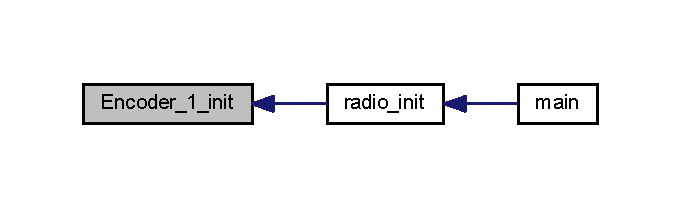
\includegraphics[width=327pt]{encoder_8h_a1b09f480da15d565de0b4acf37f40199_icgraph}
\end{center}
\end{figure}


\hypertarget{encoder_8h_a81332b0a52a42a7a7b134228f9bb3848}{}\index{encoder.\+h@{encoder.\+h}!Encoder\+\_\+2\+\_\+decoder@{Encoder\+\_\+2\+\_\+decoder}}
\index{Encoder\+\_\+2\+\_\+decoder@{Encoder\+\_\+2\+\_\+decoder}!encoder.\+h@{encoder.\+h}}
\subsubsection[{Encoder\+\_\+2\+\_\+decoder}]{\setlength{\rightskip}{0pt plus 5cm}void Encoder\+\_\+2\+\_\+decoder (
\begin{DoxyParamCaption}
\item[{void}]{}
\end{DoxyParamCaption}
)}\label{encoder_8h_a81332b0a52a42a7a7b134228f9bb3848}
\hypertarget{encoder_8h_a17708354c0e76c0422398f8dcd50dfea}{}\index{encoder.\+h@{encoder.\+h}!Encoder\+\_\+2\+\_\+get\+\_\+count@{Encoder\+\_\+2\+\_\+get\+\_\+count}}
\index{Encoder\+\_\+2\+\_\+get\+\_\+count@{Encoder\+\_\+2\+\_\+get\+\_\+count}!encoder.\+h@{encoder.\+h}}
\subsubsection[{Encoder\+\_\+2\+\_\+get\+\_\+count}]{\setlength{\rightskip}{0pt plus 5cm}int16\+\_\+t Encoder\+\_\+2\+\_\+get\+\_\+count (
\begin{DoxyParamCaption}
{}
\end{DoxyParamCaption}
)}\label{encoder_8h_a17708354c0e76c0422398f8dcd50dfea}


Hier ist ein Graph der zeigt, wo diese Funktion aufgerufen wird\+:\nopagebreak
\begin{figure}[H]
\begin{center}
\leavevmode
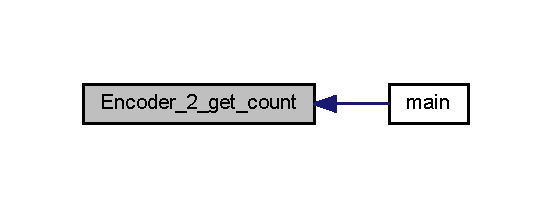
\includegraphics[width=265pt]{encoder_8h_a17708354c0e76c0422398f8dcd50dfea_icgraph}
\end{center}
\end{figure}


\hypertarget{encoder_8h_af947b4bf6e9bc6d5b580609d046789da}{}\index{encoder.\+h@{encoder.\+h}!Encoder\+\_\+2\+\_\+init@{Encoder\+\_\+2\+\_\+init}}
\index{Encoder\+\_\+2\+\_\+init@{Encoder\+\_\+2\+\_\+init}!encoder.\+h@{encoder.\+h}}
\subsubsection[{Encoder\+\_\+2\+\_\+init}]{\setlength{\rightskip}{0pt plus 5cm}void Encoder\+\_\+2\+\_\+init (
\begin{DoxyParamCaption}
\item[{void}]{}
\end{DoxyParamCaption}
)}\label{encoder_8h_af947b4bf6e9bc6d5b580609d046789da}


Hier ist ein Graph der zeigt, wo diese Funktion aufgerufen wird\+:\nopagebreak
\begin{figure}[H]
\begin{center}
\leavevmode
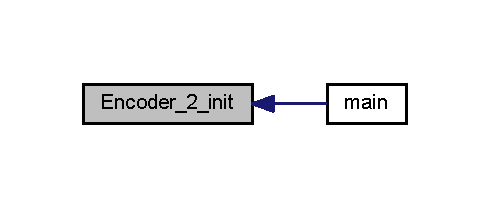
\includegraphics[width=327pt]{encoder_8h_af947b4bf6e9bc6d5b580609d046789da_icgraph}
\end{center}
\end{figure}


\hypertarget{encoder_8h_a271ca5c0624ed124f6398f408d1f3017}{}\index{encoder.\+h@{encoder.\+h}!encoder\+\_\+interrupt@{encoder\+\_\+interrupt}}
\index{encoder\+\_\+interrupt@{encoder\+\_\+interrupt}!encoder.\+h@{encoder.\+h}}
\subsubsection[{encoder\+\_\+interrupt}]{\setlength{\rightskip}{0pt plus 5cm}void encoder\+\_\+interrupt (
\begin{DoxyParamCaption}
\item[{void}]{}
\end{DoxyParamCaption}
)}\label{encoder_8h_a271ca5c0624ed124f6398f408d1f3017}
\hypertarget{encoder_8h_a136248fd00f8429933544a54b030aef9}{}\index{encoder.\+h@{encoder.\+h}!encoder\+\_\+interrupt2@{encoder\+\_\+interrupt2}}
\index{encoder\+\_\+interrupt2@{encoder\+\_\+interrupt2}!encoder.\+h@{encoder.\+h}}
\subsubsection[{encoder\+\_\+interrupt2}]{\setlength{\rightskip}{0pt plus 5cm}void encoder\+\_\+interrupt2 (
\begin{DoxyParamCaption}
\item[{void}]{}
\end{DoxyParamCaption}
)}\label{encoder_8h_a136248fd00f8429933544a54b030aef9}


Hier ist ein Graph der zeigt, wo diese Funktion aufgerufen wird\+:\nopagebreak
\begin{figure}[H]
\begin{center}
\leavevmode
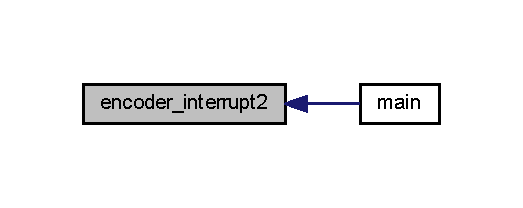
\includegraphics[width=251pt]{encoder_8h_a136248fd00f8429933544a54b030aef9_icgraph}
\end{center}
\end{figure}


\hypertarget{encoder_8h_af5a0c9bea9a0da18fa1c123af8f2877c}{}\index{encoder.\+h@{encoder.\+h}!Encoder\+\_\+\+Timer\+\_\+init@{Encoder\+\_\+\+Timer\+\_\+init}}
\index{Encoder\+\_\+\+Timer\+\_\+init@{Encoder\+\_\+\+Timer\+\_\+init}!encoder.\+h@{encoder.\+h}}
\subsubsection[{Encoder\+\_\+\+Timer\+\_\+init}]{\setlength{\rightskip}{0pt plus 5cm}void Encoder\+\_\+\+Timer\+\_\+init (
\begin{DoxyParamCaption}
\item[{void}]{}
\end{DoxyParamCaption}
)}\label{encoder_8h_af5a0c9bea9a0da18fa1c123af8f2877c}

\hypertarget{external__interrupthandler_8h}{}\section{D\+:/\+G\+I\+T/fhradiov2/driver/external\+\_\+interrupthandler.h-\/\+Dateireferenz}
\label{external__interrupthandler_8h}\index{D\+:/\+G\+I\+T/fhradiov2/driver/external\+\_\+interrupthandler.\+h@{D\+:/\+G\+I\+T/fhradiov2/driver/external\+\_\+interrupthandler.\+h}}
{\ttfamily \#include $<$msp430.\+h$>$}\\*
{\ttfamily \#include $<$stdint.\+h$>$}\\*
{\ttfamily \#include $<$settings/radio\+\_\+pin\+\_\+mapping.\+h$>$}\\*
Include-\/\+Abhängigkeitsdiagramm für external\+\_\+interrupthandler.\+h\+:
\nopagebreak
\begin{figure}[H]
\begin{center}
\leavevmode
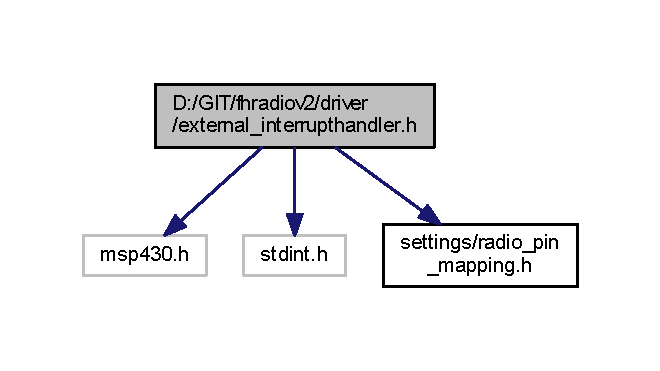
\includegraphics[width=317pt]{external__interrupthandler_8h__incl}
\end{center}
\end{figure}
Dieser Graph zeigt, welche Datei direkt oder indirekt diese Datei enthält\+:\nopagebreak
\begin{figure}[H]
\begin{center}
\leavevmode
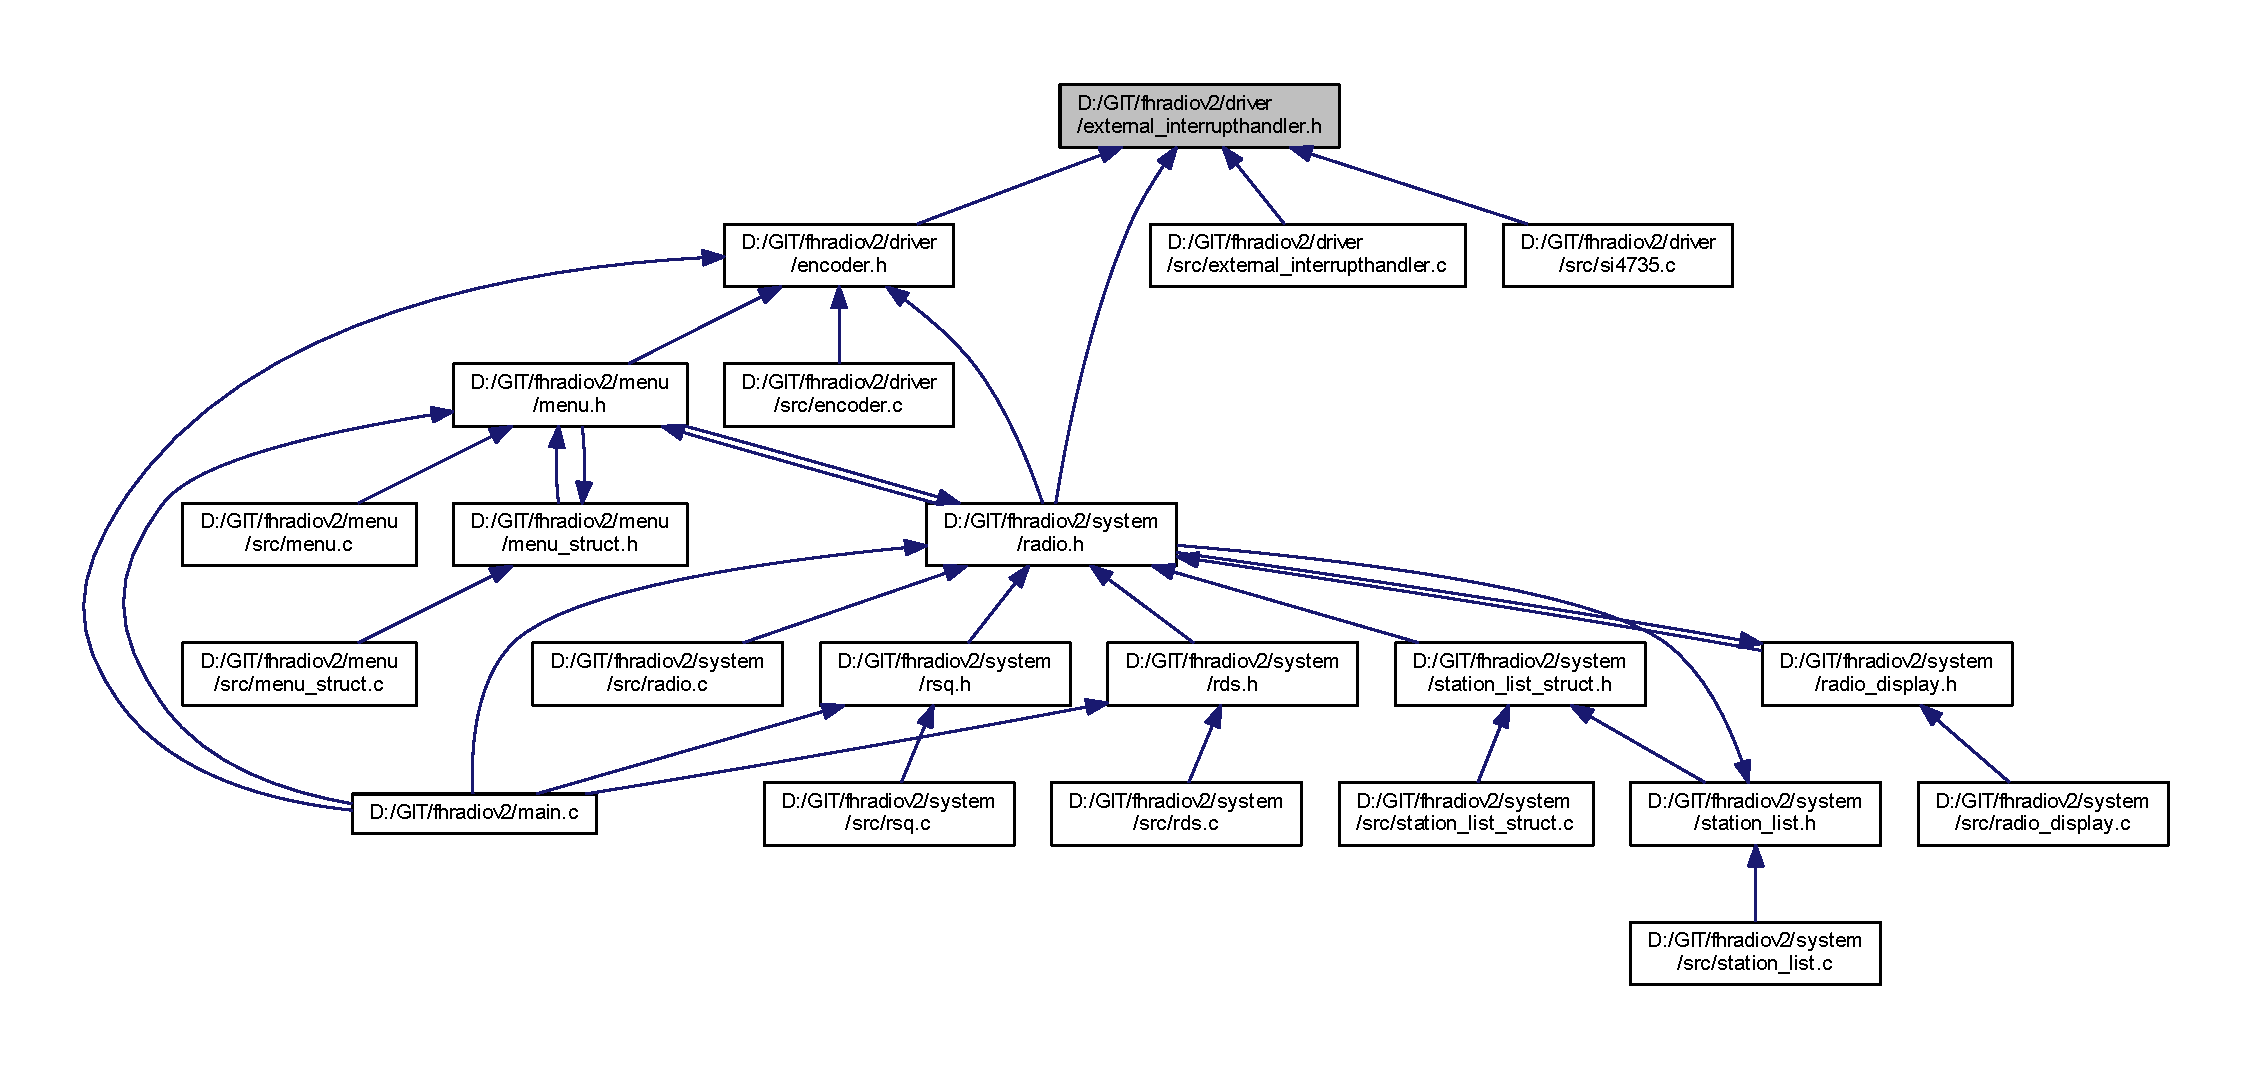
\includegraphics[width=350pt]{external__interrupthandler_8h__dep__incl}
\end{center}
\end{figure}
\subsection*{Funktionen}
\begin{DoxyCompactItemize}
\item 
uint8\+\_\+t \hyperlink{external__interrupthandler_8h_a1685394f9610006097ec45181e59563b}{ext\+\_\+interrupt\+\_\+create} (uint8\+\_\+t int\+\_\+number, void($\ast$ptrfunction)())
\item 
uint8\+\_\+t \hyperlink{external__interrupthandler_8h_a67fb5781413cf5c193be332cc6e52209}{ext\+\_\+interrupt\+\_\+disable} (uint8\+\_\+t int\+\_\+number)
\item 
uint8\+\_\+t \hyperlink{external__interrupthandler_8h_a345dfb9a7e177c5da6eb9dc5b3c82bc9}{ext\+\_\+interrupt\+\_\+enable} (uint8\+\_\+t int\+\_\+number)
\item 
uint8\+\_\+t \hyperlink{external__interrupthandler_8h_a4ee6aefa1d9150a49f8560d46f46603c}{ext\+\_\+interrupt\+\_\+delete} (uint8\+\_\+t int\+\_\+number)
\end{DoxyCompactItemize}


\subsection{Dokumentation der Funktionen}
\hypertarget{external__interrupthandler_8h_a1685394f9610006097ec45181e59563b}{}\index{external\+\_\+interrupthandler.\+h@{external\+\_\+interrupthandler.\+h}!ext\+\_\+interrupt\+\_\+create@{ext\+\_\+interrupt\+\_\+create}}
\index{ext\+\_\+interrupt\+\_\+create@{ext\+\_\+interrupt\+\_\+create}!external\+\_\+interrupthandler.\+h@{external\+\_\+interrupthandler.\+h}}
\subsubsection[{ext\+\_\+interrupt\+\_\+create}]{\setlength{\rightskip}{0pt plus 5cm}uint8\+\_\+t ext\+\_\+interrupt\+\_\+create (
\begin{DoxyParamCaption}
\item[{uint8\+\_\+t}]{int\+\_\+number, }
\item[{void($\ast$)()}]{ptrfunction}
\end{DoxyParamCaption}
)}\label{external__interrupthandler_8h_a1685394f9610006097ec45181e59563b}


Definiert in Zeile 16 der Datei external\+\_\+interrupthandler.\+c.


\begin{DoxyCode}
17 \{
18     \textcolor{keywordflow}{if}(int\_number > 15) \{
19         \textcolor{keywordflow}{return} 0xFF;
20     \}
21     \hyperlink{external__interrupthandler_8c_ac6a491a811bf236b0743231661f43b10}{ext\_int\_handler}[int\_number] = (\hyperlink{external__interrupthandler_8c_a49f7f660c4305c86e6dc6da9cdc7a570}{ptrfunc})ptrfunction;
22 
23     \textcolor{keywordflow}{return} 0;
24 \}
\end{DoxyCode}


Hier ist ein Graph der zeigt, wo diese Funktion aufgerufen wird\+:\nopagebreak
\begin{figure}[H]
\begin{center}
\leavevmode
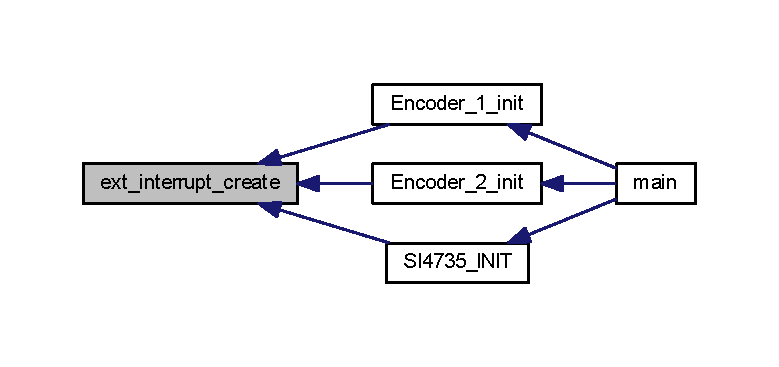
\includegraphics[width=350pt]{external__interrupthandler_8h_a1685394f9610006097ec45181e59563b_icgraph}
\end{center}
\end{figure}


\hypertarget{external__interrupthandler_8h_a4ee6aefa1d9150a49f8560d46f46603c}{}\index{external\+\_\+interrupthandler.\+h@{external\+\_\+interrupthandler.\+h}!ext\+\_\+interrupt\+\_\+delete@{ext\+\_\+interrupt\+\_\+delete}}
\index{ext\+\_\+interrupt\+\_\+delete@{ext\+\_\+interrupt\+\_\+delete}!external\+\_\+interrupthandler.\+h@{external\+\_\+interrupthandler.\+h}}
\subsubsection[{ext\+\_\+interrupt\+\_\+delete}]{\setlength{\rightskip}{0pt plus 5cm}uint8\+\_\+t ext\+\_\+interrupt\+\_\+delete (
\begin{DoxyParamCaption}
\item[{uint8\+\_\+t}]{int\+\_\+number}
\end{DoxyParamCaption}
)}\label{external__interrupthandler_8h_a4ee6aefa1d9150a49f8560d46f46603c}


Definiert in Zeile 26 der Datei external\+\_\+interrupthandler.\+c.


\begin{DoxyCode}
27 \{
28     \textcolor{keywordflow}{if}(int\_number > 15) \{
29         \textcolor{keywordflow}{return} 0xFF;
30     \}
31     \hyperlink{external__interrupthandler_8c_ac6a491a811bf236b0743231661f43b10}{ext\_int\_handler}[int\_number] = 0;
32 
33     \textcolor{keywordflow}{return} 0;
34 \}
\end{DoxyCode}
\hypertarget{external__interrupthandler_8h_a67fb5781413cf5c193be332cc6e52209}{}\index{external\+\_\+interrupthandler.\+h@{external\+\_\+interrupthandler.\+h}!ext\+\_\+interrupt\+\_\+disable@{ext\+\_\+interrupt\+\_\+disable}}
\index{ext\+\_\+interrupt\+\_\+disable@{ext\+\_\+interrupt\+\_\+disable}!external\+\_\+interrupthandler.\+h@{external\+\_\+interrupthandler.\+h}}
\subsubsection[{ext\+\_\+interrupt\+\_\+disable}]{\setlength{\rightskip}{0pt plus 5cm}uint8\+\_\+t ext\+\_\+interrupt\+\_\+disable (
\begin{DoxyParamCaption}
\item[{uint8\+\_\+t}]{int\+\_\+number}
\end{DoxyParamCaption}
)}\label{external__interrupthandler_8h_a67fb5781413cf5c193be332cc6e52209}


Definiert in Zeile 49 der Datei external\+\_\+interrupthandler.\+c.


\begin{DoxyCode}
50 \{
51     \textcolor{keywordflow}{if}(int\_number/8) \{
52         P2IE &= ~(1 << int\_number % 8);
53     \}
54     \textcolor{keywordflow}{else} \{
55         P1IE &= ~(1 << int\_number % 8);
56     \}
57     \textcolor{keywordflow}{return} 0;
58 \}
\end{DoxyCode}


Hier ist ein Graph der zeigt, wo diese Funktion aufgerufen wird\+:
\nopagebreak
\begin{figure}[H]
\begin{center}
\leavevmode
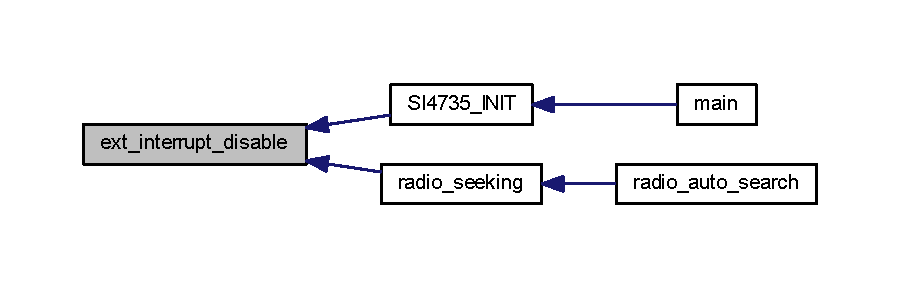
\includegraphics[width=350pt]{external__interrupthandler_8h_a67fb5781413cf5c193be332cc6e52209_icgraph}
\end{center}
\end{figure}


\hypertarget{external__interrupthandler_8h_a345dfb9a7e177c5da6eb9dc5b3c82bc9}{}\index{external\+\_\+interrupthandler.\+h@{external\+\_\+interrupthandler.\+h}!ext\+\_\+interrupt\+\_\+enable@{ext\+\_\+interrupt\+\_\+enable}}
\index{ext\+\_\+interrupt\+\_\+enable@{ext\+\_\+interrupt\+\_\+enable}!external\+\_\+interrupthandler.\+h@{external\+\_\+interrupthandler.\+h}}
\subsubsection[{ext\+\_\+interrupt\+\_\+enable}]{\setlength{\rightskip}{0pt plus 5cm}uint8\+\_\+t ext\+\_\+interrupt\+\_\+enable (
\begin{DoxyParamCaption}
\item[{uint8\+\_\+t}]{int\+\_\+number}
\end{DoxyParamCaption}
)}\label{external__interrupthandler_8h_a345dfb9a7e177c5da6eb9dc5b3c82bc9}


Definiert in Zeile 36 der Datei external\+\_\+interrupthandler.\+c.


\begin{DoxyCode}
37 \{
38     \textcolor{keywordflow}{if}(int\_number/8) \{
39         P2IFG &= ~(1 << (int\_number % 8));
40         P2IE |= (1 << (int\_number % 8));
41     \}
42     \textcolor{keywordflow}{else} \{
43         P1IFG &= ~(1 << (int\_number % 8));
44         P1IE |= (1 << (int\_number % 8));
45     \}
46     \textcolor{keywordflow}{return} 0;
47 \}
\end{DoxyCode}


Hier ist ein Graph der zeigt, wo diese Funktion aufgerufen wird\+:
\nopagebreak
\begin{figure}[H]
\begin{center}
\leavevmode
\includegraphics[width=350pt]{external__interrupthandler_8h_a345dfb9a7e177c5da6eb9dc5b3c82bc9_icgraph}
\end{center}
\end{figure}



\hypertarget{flash_8h}{}\section{D\+:/\+G\+I\+T/fhradiov2/driver/flash.h-\/\+Dateireferenz}
\label{flash_8h}\index{D\+:/\+G\+I\+T/fhradiov2/driver/flash.\+h@{D\+:/\+G\+I\+T/fhradiov2/driver/flash.\+h}}
{\ttfamily \#include $<$stdint.\+h$>$}\\*
{\ttfamily \#include $<$string.\+h$>$}\\*
{\ttfamily \#include $<$msp430.\+h$>$}\\*
Include-\/\+Abhängigkeitsdiagramm für flash.\+h\+:\nopagebreak
\begin{figure}[H]
\begin{center}
\leavevmode
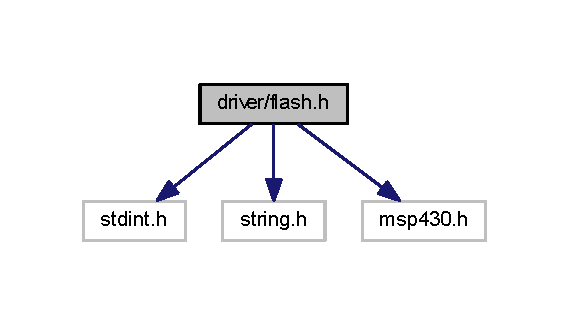
\includegraphics[width=237pt]{flash_8h__incl}
\end{center}
\end{figure}
Dieser Graph zeigt, welche Datei direkt oder indirekt diese Datei enthält\+:\nopagebreak
\begin{figure}[H]
\begin{center}
\leavevmode
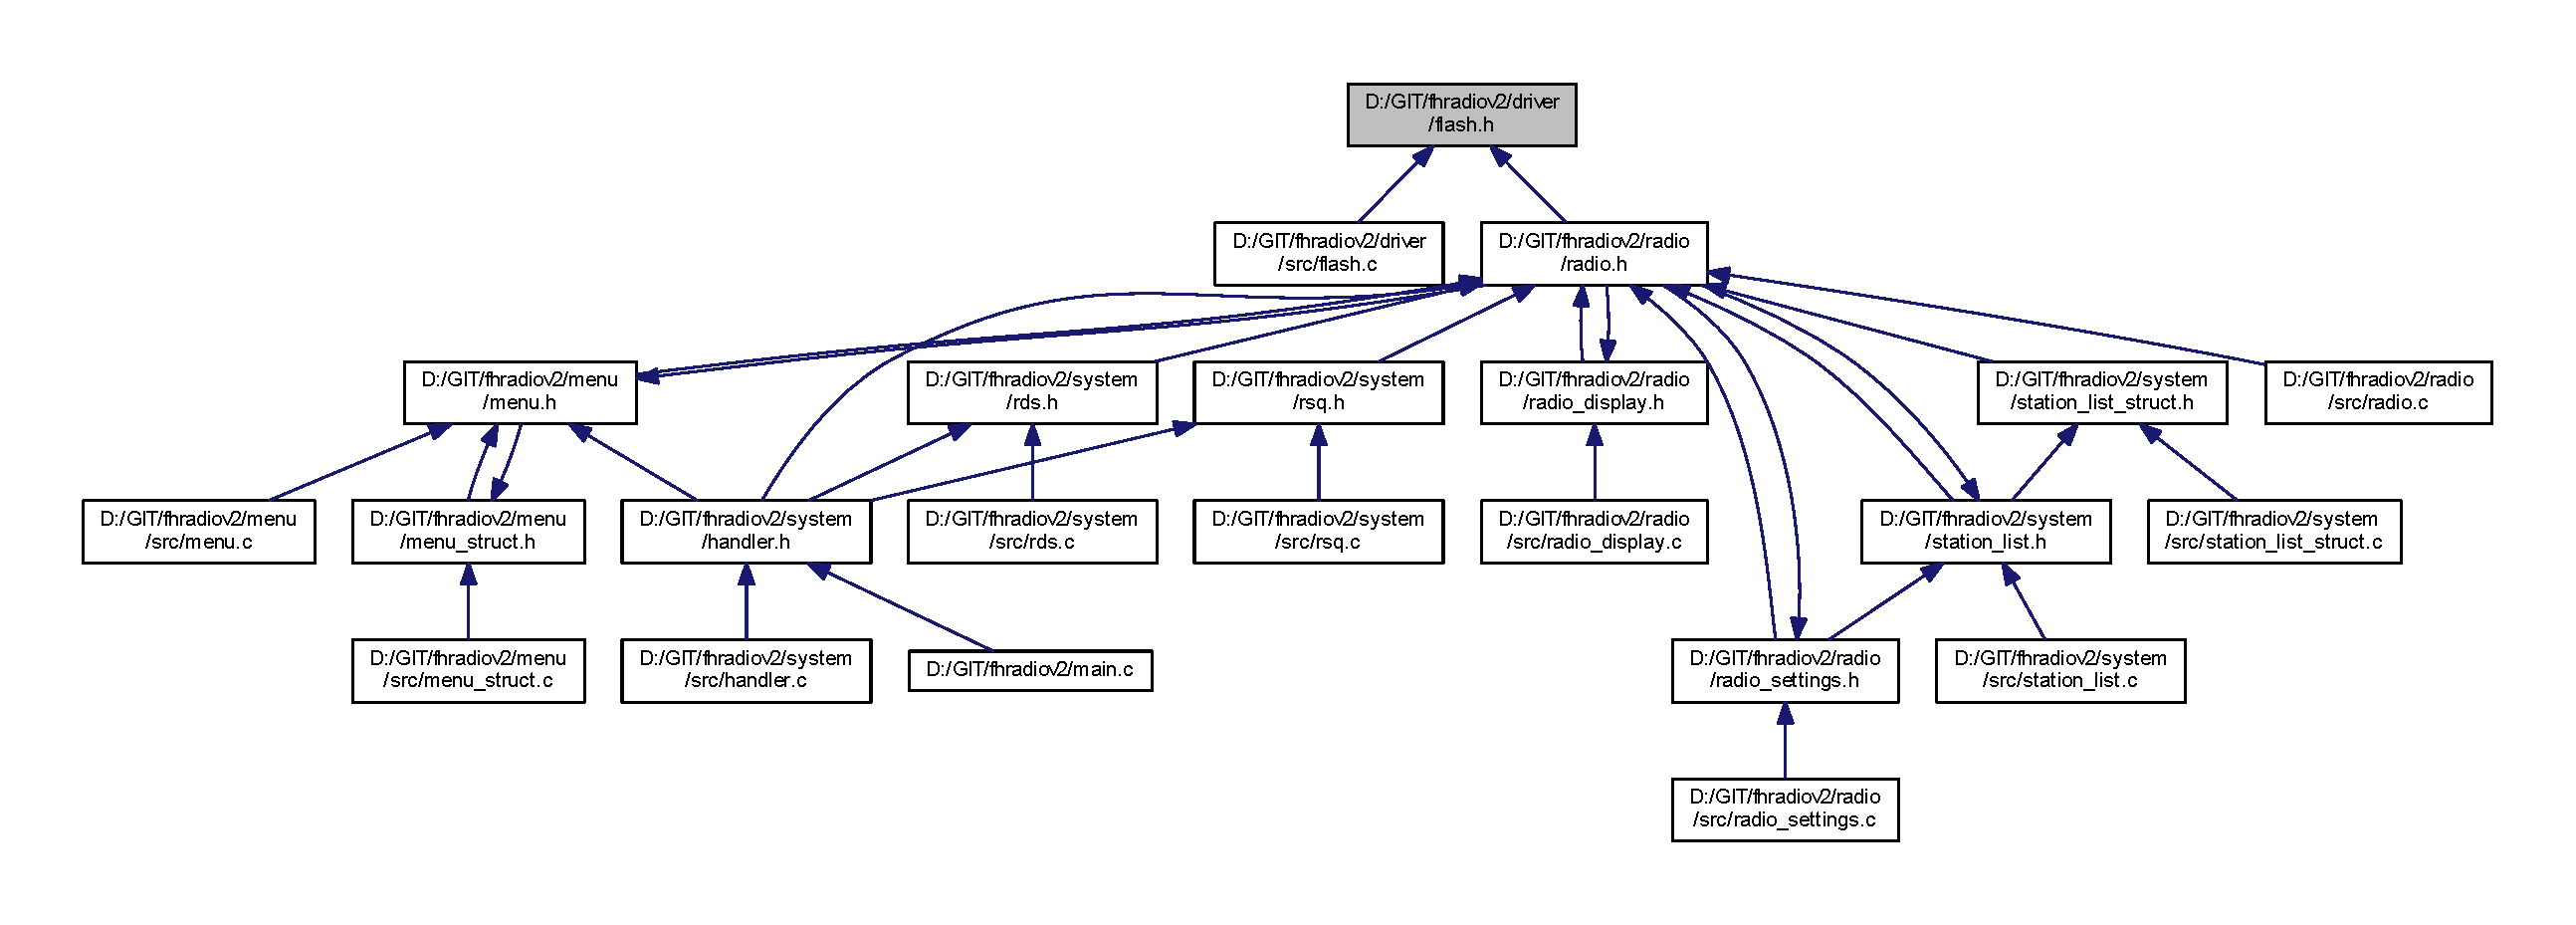
\includegraphics[width=350pt]{flash_8h__dep__incl}
\end{center}
\end{figure}
\subsection*{Makrodefinitionen}
\begin{DoxyCompactItemize}
\item 
\#define \hyperlink{flash_8h_aacc1626c22c9bd0b71666e386e59c8aa}{F\+L\+A\+S\+H\+\_\+\+A\+D\+R\+\_\+\+S\+T\+A\+R\+T}~0x1000
\item 
\#define \hyperlink{flash_8h_acc6c9e893edc4bef8dbe6e157c926a89}{F\+L\+A\+S\+H\+\_\+\+S\+E\+G\+\_\+\+S\+I\+Z\+E}~0x0040
\item 
\#define \hyperlink{flash_8h_a6d0dc3446b513aa476db4b376aa92068}{F\+L\+A\+S\+H\+\_\+\+A\+D\+R\+\_\+\+S\+T\+O\+P}~0x10\+F\+F
\end{DoxyCompactItemize}
\subsection*{Funktionen}
\begin{DoxyCompactItemize}
\item 
uint8\+\_\+t \hyperlink{flash_8h_a936ded19cea6a94beca2b32349a9ac2c}{flash\+\_\+store} (void $\ast$data, uint8\+\_\+t size, uint16\+\_\+t pos)
\item 
uint8\+\_\+t \hyperlink{flash_8h_ad9d8a7cadb959b139fea7654d539714a}{flash\+\_\+read} (void $\ast$data, uint8\+\_\+t size, uint16\+\_\+t pos)
\item 
void \hyperlink{flash_8h_a4b761d1814aa17114267763d71266513}{flash\+\_\+erase} (uint8\+\_\+t $\ast$Flash\+\_\+ptr)
\end{DoxyCompactItemize}


\subsection{Makro-\/\+Dokumentation}
\hypertarget{flash_8h_aacc1626c22c9bd0b71666e386e59c8aa}{}\index{flash.\+h@{flash.\+h}!F\+L\+A\+S\+H\+\_\+\+A\+D\+R\+\_\+\+S\+T\+A\+R\+T@{F\+L\+A\+S\+H\+\_\+\+A\+D\+R\+\_\+\+S\+T\+A\+R\+T}}
\index{F\+L\+A\+S\+H\+\_\+\+A\+D\+R\+\_\+\+S\+T\+A\+R\+T@{F\+L\+A\+S\+H\+\_\+\+A\+D\+R\+\_\+\+S\+T\+A\+R\+T}!flash.\+h@{flash.\+h}}
\subsubsection[{F\+L\+A\+S\+H\+\_\+\+A\+D\+R\+\_\+\+S\+T\+A\+R\+T}]{\setlength{\rightskip}{0pt plus 5cm}\#define F\+L\+A\+S\+H\+\_\+\+A\+D\+R\+\_\+\+S\+T\+A\+R\+T~0x1000}\label{flash_8h_aacc1626c22c9bd0b71666e386e59c8aa}


Definiert in Zeile 11 der Datei flash.\+h.

\hypertarget{flash_8h_a6d0dc3446b513aa476db4b376aa92068}{}\index{flash.\+h@{flash.\+h}!F\+L\+A\+S\+H\+\_\+\+A\+D\+R\+\_\+\+S\+T\+O\+P@{F\+L\+A\+S\+H\+\_\+\+A\+D\+R\+\_\+\+S\+T\+O\+P}}
\index{F\+L\+A\+S\+H\+\_\+\+A\+D\+R\+\_\+\+S\+T\+O\+P@{F\+L\+A\+S\+H\+\_\+\+A\+D\+R\+\_\+\+S\+T\+O\+P}!flash.\+h@{flash.\+h}}
\subsubsection[{F\+L\+A\+S\+H\+\_\+\+A\+D\+R\+\_\+\+S\+T\+O\+P}]{\setlength{\rightskip}{0pt plus 5cm}\#define F\+L\+A\+S\+H\+\_\+\+A\+D\+R\+\_\+\+S\+T\+O\+P~0x10\+F\+F}\label{flash_8h_a6d0dc3446b513aa476db4b376aa92068}


Definiert in Zeile 13 der Datei flash.\+h.

\hypertarget{flash_8h_acc6c9e893edc4bef8dbe6e157c926a89}{}\index{flash.\+h@{flash.\+h}!F\+L\+A\+S\+H\+\_\+\+S\+E\+G\+\_\+\+S\+I\+Z\+E@{F\+L\+A\+S\+H\+\_\+\+S\+E\+G\+\_\+\+S\+I\+Z\+E}}
\index{F\+L\+A\+S\+H\+\_\+\+S\+E\+G\+\_\+\+S\+I\+Z\+E@{F\+L\+A\+S\+H\+\_\+\+S\+E\+G\+\_\+\+S\+I\+Z\+E}!flash.\+h@{flash.\+h}}
\subsubsection[{F\+L\+A\+S\+H\+\_\+\+S\+E\+G\+\_\+\+S\+I\+Z\+E}]{\setlength{\rightskip}{0pt plus 5cm}\#define F\+L\+A\+S\+H\+\_\+\+S\+E\+G\+\_\+\+S\+I\+Z\+E~0x0040}\label{flash_8h_acc6c9e893edc4bef8dbe6e157c926a89}


Definiert in Zeile 12 der Datei flash.\+h.



\subsection{Dokumentation der Funktionen}
\hypertarget{flash_8h_a4b761d1814aa17114267763d71266513}{}\index{flash.\+h@{flash.\+h}!flash\+\_\+erase@{flash\+\_\+erase}}
\index{flash\+\_\+erase@{flash\+\_\+erase}!flash.\+h@{flash.\+h}}
\subsubsection[{flash\+\_\+erase}]{\setlength{\rightskip}{0pt plus 5cm}void flash\+\_\+erase (
\begin{DoxyParamCaption}
\item[{uint8\+\_\+t $\ast$}]{Flash\+\_\+ptr}
\end{DoxyParamCaption}
)}\label{flash_8h_a4b761d1814aa17114267763d71266513}


Definiert in Zeile 71 der Datei flash.\+c.


\begin{DoxyCode}
72 \{
73     \textcolor{keywordflow}{while}(BUSY & FCTL3);
74     FCTL1 = FWKEY + ERASE;                   \textcolor{comment}{// Set Erase bit}
75     FCTL3 = FWKEY;                           \textcolor{comment}{// Clear Lock bit}
76     *Flash\_ptr = 0;                          \textcolor{comment}{// Dummy write to erase Flash segment}
77     \textcolor{keywordflow}{while}(BUSY & FCTL3);
78     FCTL1 = FWKEY;                           \textcolor{comment}{// Clear WRT bit}
79     FCTL3 = FWKEY + LOCK;                    \textcolor{comment}{// Set LOCK bit}
80 \}
\end{DoxyCode}
\hypertarget{flash_8h_ad9d8a7cadb959b139fea7654d539714a}{}\index{flash.\+h@{flash.\+h}!flash\+\_\+read@{flash\+\_\+read}}
\index{flash\+\_\+read@{flash\+\_\+read}!flash.\+h@{flash.\+h}}
\subsubsection[{flash\+\_\+read}]{\setlength{\rightskip}{0pt plus 5cm}uint8\+\_\+t flash\+\_\+read (
\begin{DoxyParamCaption}
\item[{void $\ast$}]{data, }
\item[{uint8\+\_\+t}]{size, }
\item[{uint16\+\_\+t}]{pos}
\end{DoxyParamCaption}
)}\label{flash_8h_ad9d8a7cadb959b139fea7654d539714a}


Definiert in Zeile 63 der Datei flash.\+c.


\begin{DoxyCode}
64 \{
65     uint8\_t *Flash\_ptr = 0;
66     Flash\_ptr = (uint8\_t *)pos;
67     memcpy(data, Flash\_ptr, size);
68     \textcolor{keywordflow}{return} 0;
69 \}
\end{DoxyCode}


Hier ist ein Graph der zeigt, wo diese Funktion aufgerufen wird\+:
\nopagebreak
\begin{figure}[H]
\begin{center}
\leavevmode
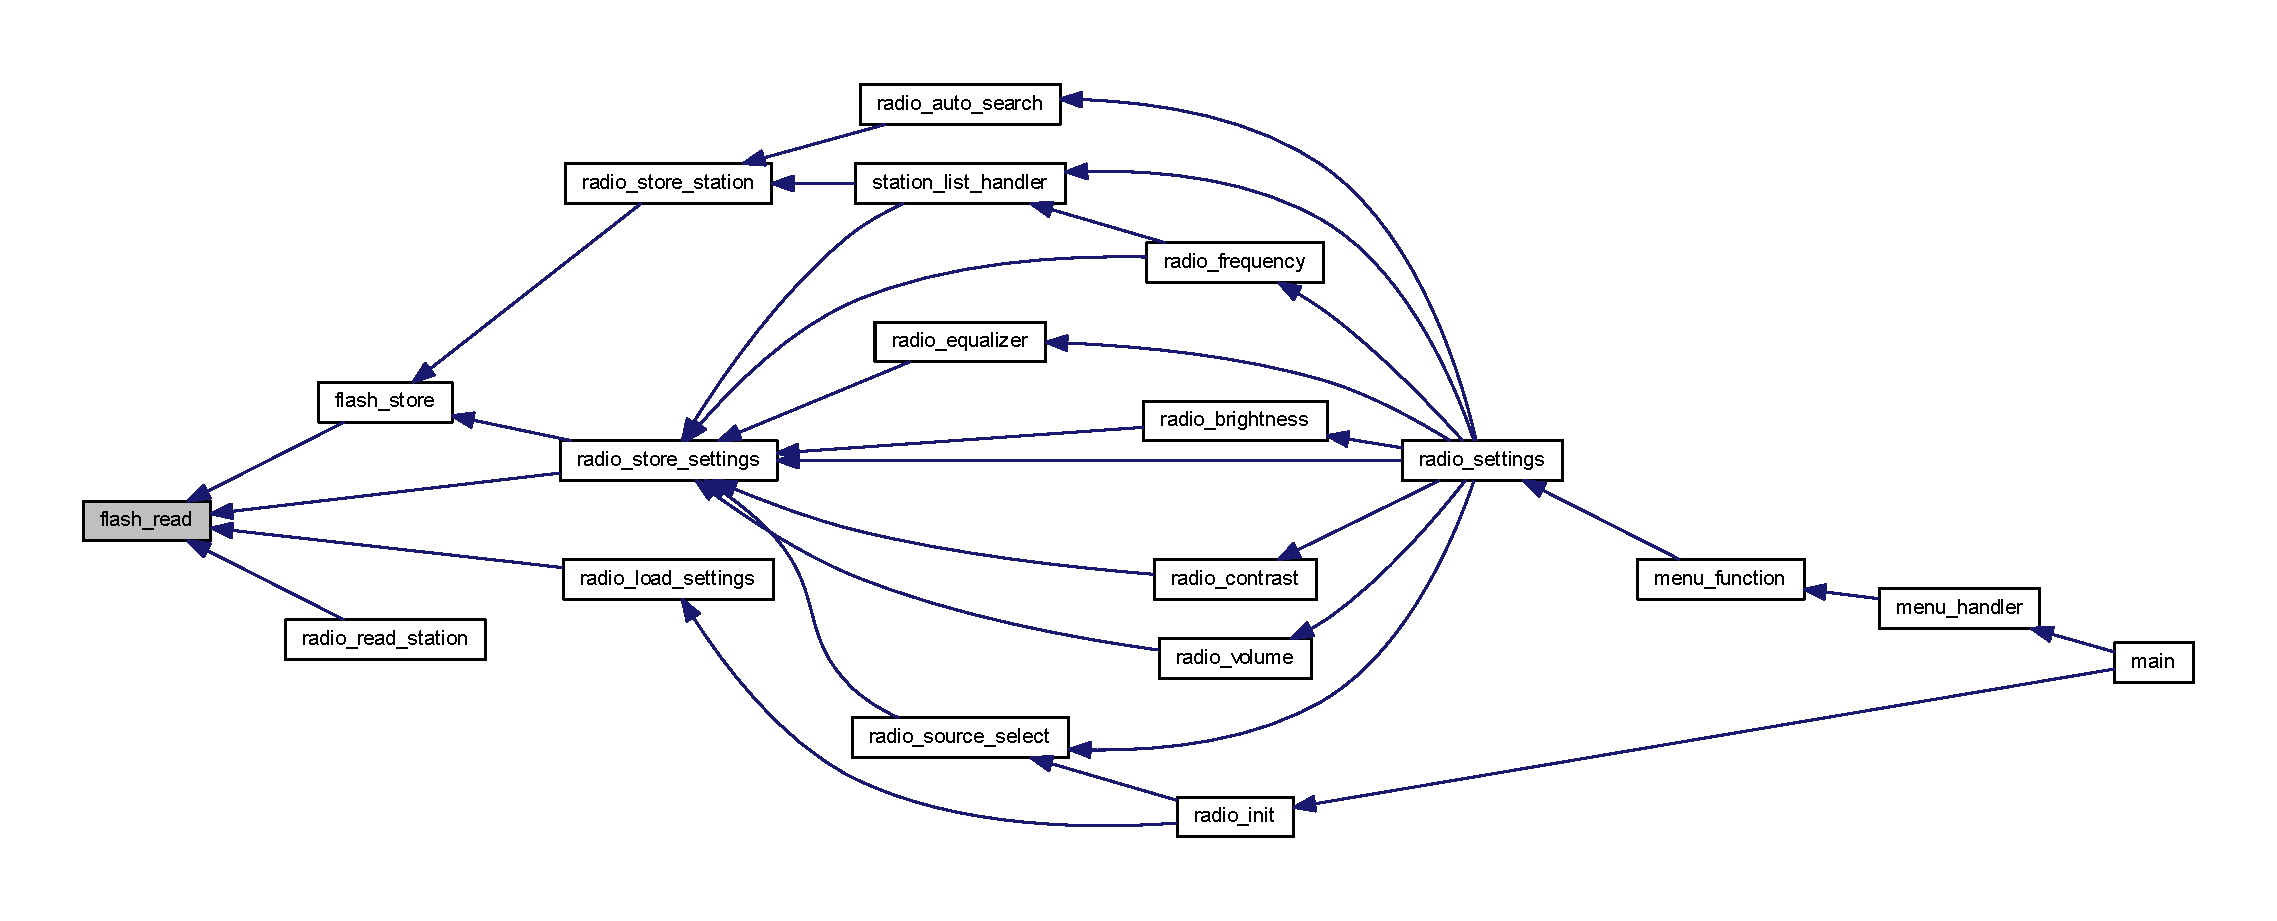
\includegraphics[width=350pt]{flash_8h_ad9d8a7cadb959b139fea7654d539714a_icgraph}
\end{center}
\end{figure}


\hypertarget{flash_8h_a936ded19cea6a94beca2b32349a9ac2c}{}\index{flash.\+h@{flash.\+h}!flash\+\_\+store@{flash\+\_\+store}}
\index{flash\+\_\+store@{flash\+\_\+store}!flash.\+h@{flash.\+h}}
\subsubsection[{flash\+\_\+store}]{\setlength{\rightskip}{0pt plus 5cm}uint8\+\_\+t flash\+\_\+store (
\begin{DoxyParamCaption}
\item[{void $\ast$}]{data, }
\item[{uint8\+\_\+t}]{size, }
\item[{uint16\+\_\+t}]{pos}
\end{DoxyParamCaption}
)}\label{flash_8h_a936ded19cea6a94beca2b32349a9ac2c}


Definiert in Zeile 11 der Datei flash.\+c.


\begin{DoxyCode}
12 \{
13     \_\_disable\_interrupt();
14     uint8\_t *Flash\_ptr = (uint8\_t *)\hyperlink{flash_8h_aacc1626c22c9bd0b71666e386e59c8aa}{FLASH\_ADR\_START};
15     uint8\_t seg\_store[\hyperlink{flash_8h_acc6c9e893edc4bef8dbe6e157c926a89}{FLASH\_SEG\_SIZE}];
16     \textcolor{keyword}{register} uint8\_t i = 0;
17 
18     Flash\_ptr = (uint8\_t *)pos;
19 
20     pos -= \hyperlink{flash_8h_aacc1626c22c9bd0b71666e386e59c8aa}{FLASH\_ADR\_START};
21 
22     \textcolor{keywordflow}{switch}(pos / \hyperlink{flash_8h_acc6c9e893edc4bef8dbe6e157c926a89}{FLASH\_SEG\_SIZE}) \{
23         \textcolor{keywordflow}{case} 0:
24             \hyperlink{flash_8c_ad9d8a7cadb959b139fea7654d539714a}{flash\_read}(seg\_store, (uint8\_t)\hyperlink{flash_8h_acc6c9e893edc4bef8dbe6e157c926a89}{FLASH\_SEG\_SIZE}, 
      \hyperlink{flash_8h_aacc1626c22c9bd0b71666e386e59c8aa}{FLASH\_ADR\_START});
25             \textcolor{keywordflow}{break};
26         \textcolor{keywordflow}{case} 1:
27             \hyperlink{flash_8c_ad9d8a7cadb959b139fea7654d539714a}{flash\_read}(seg\_store, (uint8\_t)\hyperlink{flash_8h_acc6c9e893edc4bef8dbe6e157c926a89}{FLASH\_SEG\_SIZE}, 
      \hyperlink{flash_8h_aacc1626c22c9bd0b71666e386e59c8aa}{FLASH\_ADR\_START} + FLASH\_SEG\_SIZE);
28             \textcolor{keywordflow}{break};
29         \textcolor{keywordflow}{case} 2:
30             \hyperlink{flash_8c_ad9d8a7cadb959b139fea7654d539714a}{flash\_read}(seg\_store, (uint8\_t)\hyperlink{flash_8h_acc6c9e893edc4bef8dbe6e157c926a89}{FLASH\_SEG\_SIZE}, 
      \hyperlink{flash_8h_aacc1626c22c9bd0b71666e386e59c8aa}{FLASH\_ADR\_START} + 2 * FLASH\_SEG\_SIZE);
31             \textcolor{keywordflow}{break};
32         \textcolor{keywordflow}{default}:
33             \textcolor{keywordflow}{return} 0xFE;
34     \}
35 
36     pos %= \hyperlink{flash_8h_acc6c9e893edc4bef8dbe6e157c926a89}{FLASH\_SEG\_SIZE};
37     \textcolor{keywordflow}{if}(size + pos > \hyperlink{flash_8h_acc6c9e893edc4bef8dbe6e157c926a89}{FLASH\_SEG\_SIZE}) \{
38         \textcolor{keywordflow}{return} 0xFF;
39     \}
40 
41     memcpy(seg\_store + pos, data, size);
42 
43     FCTL1 = FWKEY + ERASE; \textcolor{comment}{// Set Erase bit}
44     FCTL3 = FWKEY; \textcolor{comment}{// Clear Lock bit}
45     *Flash\_ptr = 0; \textcolor{comment}{// Dummy write to erase Flash segment}
46     Flash\_ptr -= pos;
47 
48     FCTL1 = FWKEY + WRT;                \textcolor{comment}{// Set WRT bit for write operation}
49     \textcolor{comment}{//FCTL3 = FWKEY;                            // Clear Lock bit}
50 
51     \textcolor{keywordflow}{for}(i = 0; i < (uint8\_t)\hyperlink{flash_8h_acc6c9e893edc4bef8dbe6e157c926a89}{FLASH\_SEG\_SIZE}; i++) \{
52         Flash\_ptr[i] = seg\_store[i];        \textcolor{comment}{// Write value to flash}
53     \}
54 
55     FCTL1 = FWKEY;                  \textcolor{comment}{// Clear WRT bit}
56     FCTL3 = FWKEY + LOCK;                       \textcolor{comment}{// Set LOCK bit}
57 
58     \_\_enable\_interrupt();
59 
60     \textcolor{keywordflow}{return} 0;
61 \}
\end{DoxyCode}


Hier ist ein Graph, der zeigt, was diese Funktion aufruft\+:
\nopagebreak
\begin{figure}[H]
\begin{center}
\leavevmode
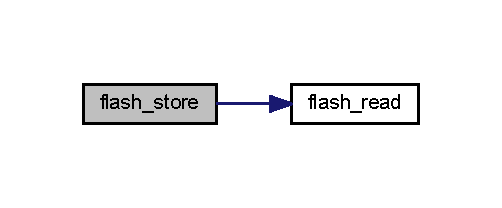
\includegraphics[width=241pt]{flash_8h_a936ded19cea6a94beca2b32349a9ac2c_cgraph}
\end{center}
\end{figure}




Hier ist ein Graph der zeigt, wo diese Funktion aufgerufen wird\+:
\nopagebreak
\begin{figure}[H]
\begin{center}
\leavevmode
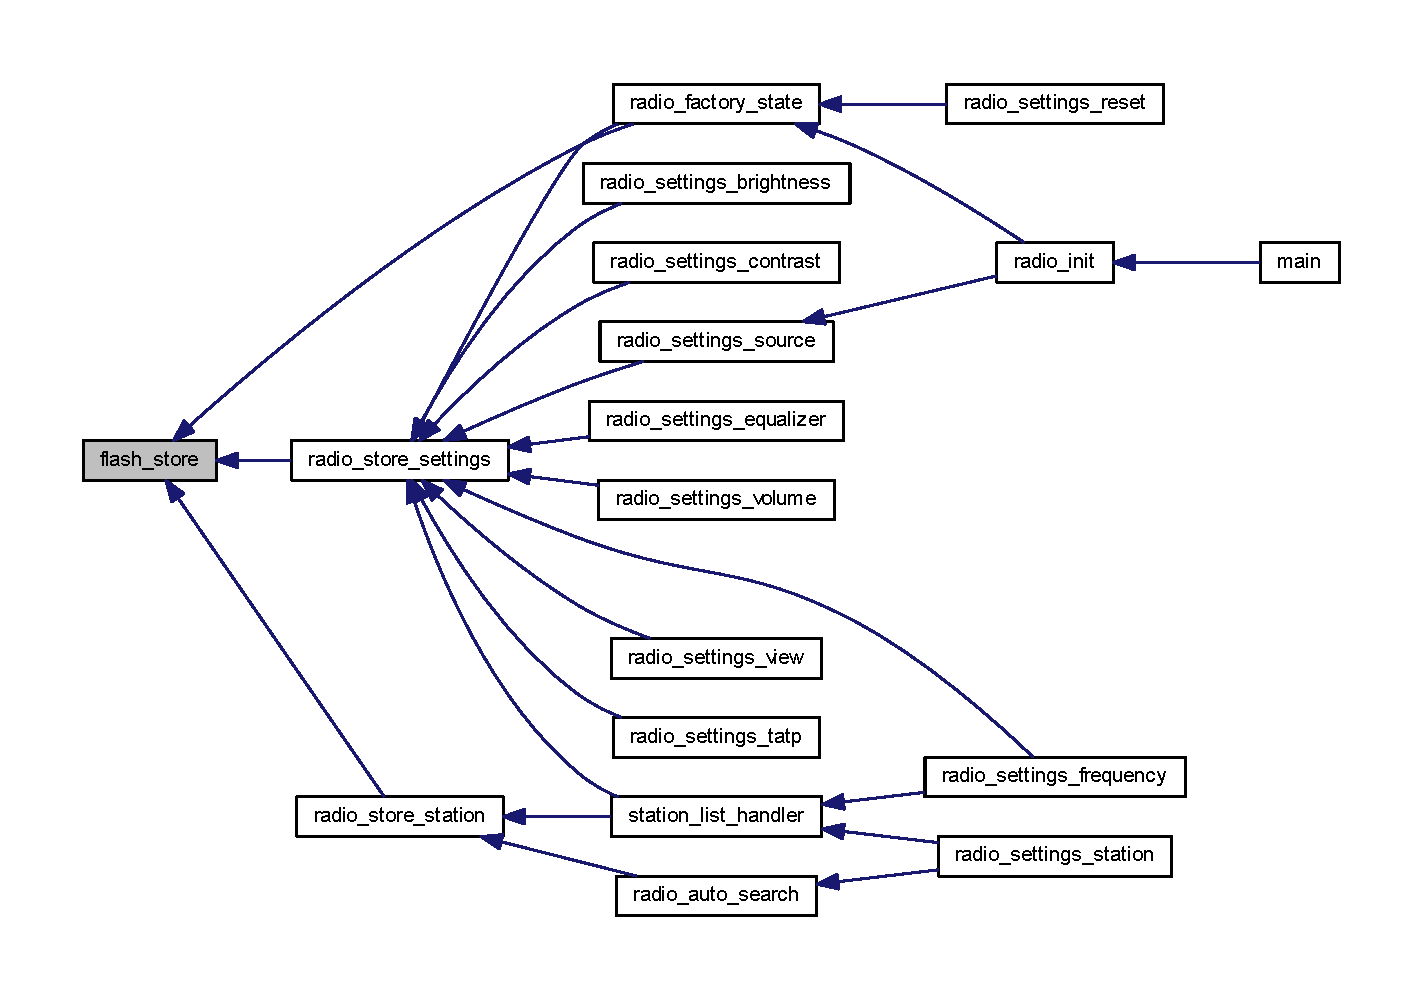
\includegraphics[width=350pt]{flash_8h_a936ded19cea6a94beca2b32349a9ac2c_icgraph}
\end{center}
\end{figure}



\hypertarget{i2c_8h}{}\section{D\+:/\+G\+I\+T/fhradiov2/driver/i2c.h-\/\+Dateireferenz}
\label{i2c_8h}\index{D\+:/\+G\+I\+T/fhradiov2/driver/i2c.\+h@{D\+:/\+G\+I\+T/fhradiov2/driver/i2c.\+h}}


I2\+C implemtation for M\+S\+P430\+G2553, interrupt based. ~\newline
 This implemtation based on examples from Texas Instruments slaa382. ~\newline
 For more information see link below.  


{\ttfamily \#include $<$stdint.\+h$>$}\\*
{\ttfamily \#include $<$msp430.\+h$>$}\\*
{\ttfamily \#include $<$stdlib.\+h$>$}\\*
{\ttfamily \#include $<$stdarg.\+h$>$}\\*
{\ttfamily \#include $<$driver/timer.\+h$>$}\\*
Include-\/\+Abhängigkeitsdiagramm für i2c.\+h\+:
\nopagebreak
\begin{figure}[H]
\begin{center}
\leavevmode
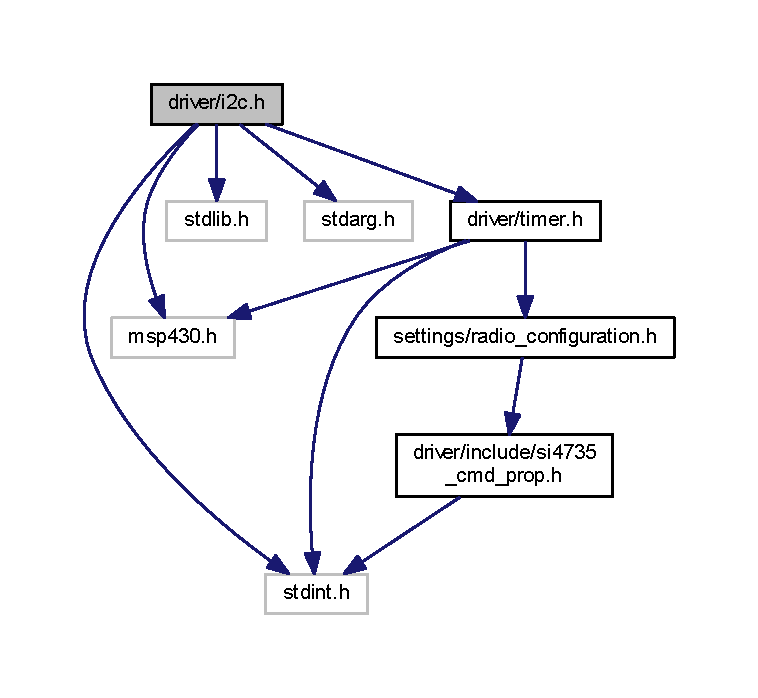
\includegraphics[width=350pt]{i2c_8h__incl}
\end{center}
\end{figure}
Dieser Graph zeigt, welche Datei direkt oder indirekt diese Datei enthält\+:
\nopagebreak
\begin{figure}[H]
\begin{center}
\leavevmode
\includegraphics[width=350pt]{i2c_8h__dep__incl}
\end{center}
\end{figure}
\subsection*{Makrodefinitionen}
\begin{DoxyCompactItemize}
\item 
\#define \hyperlink{i2c_8h_abb6e116b2f7cc724b26d78a65303ccc6}{V\+A\+R\+I\+A\+D\+I\+C\+\_\+\+I\+M\+P\+L\+E\+M\+E\+N\+T\+A\+T\+I\+O\+N}~0
\item 
\#define \hyperlink{i2c_8h_afd2ccfc308be2593bb7540863b903d67}{I2\+C\+\_\+\+M\+A\+X\+\_\+\+A\+R\+G\+S}~10
\end{DoxyCompactItemize}
\subsection*{Aufzählungen}
\begin{DoxyCompactItemize}
\item 
enum \hyperlink{i2c_8h_aaaea3962492fd5ad1e43cba027d949d5}{I2\+C\+\_\+\+C\+R\+T\+L\+\_\+\+C\+M\+D} \{ \hyperlink{i2c_8h_aaaea3962492fd5ad1e43cba027d949d5a679ee5320d66c8322e310daeb2ee99b8}{S\+T\+O\+P} = 0, 
\hyperlink{i2c_8h_aaaea3962492fd5ad1e43cba027d949d5a807d17ddb75240ddeede2c54fd79bd40}{R\+E\+P\+T}
 \}
\begin{DoxyCompactList}\small\item\em Control command for sendig a S\+T\+O\+P condtion or repeated start. \end{DoxyCompactList}\item 
enum \hyperlink{i2c_8h_a8f12d82f4a490ef04de32baf91363d9b}{I2\+C\+\_\+\+C\+R\+T\+L\+\_\+\+S\+T\+A\+T\+S} \{ \hyperlink{i2c_8h_a8f12d82f4a490ef04de32baf91363d9bafd6a0e4343048b10646dd2976cc5ad18}{I\+D\+L\+E} = 0, 
\hyperlink{i2c_8h_a8f12d82f4a490ef04de32baf91363d9bad208fa8c08969a9d78096817bf0a6377}{T\+R\+A\+N\+S\+M\+I\+T}, 
\hyperlink{i2c_8h_a8f12d82f4a490ef04de32baf91363d9ba563f8ed00490ea22ea2605d9571dada8}{R\+E\+C\+E\+I\+V\+E}, 
\hyperlink{i2c_8h_a8f12d82f4a490ef04de32baf91363d9ba2fd6f336d08340583bd620a7f5694c90}{E\+R\+R\+O\+R}
 \}
\begin{DoxyCompactList}\small\item\em Give back a status of I2\+C module. \end{DoxyCompactList}\end{DoxyCompactItemize}
\subsection*{Funktionen}
\begin{DoxyCompactItemize}
\item 
uint8\+\_\+t \hyperlink{i2c_8h_a1ef889b72b844429bc81225d7b6f4f2e}{i2c\+\_\+init} (uint16\+\_\+t smclk\+\_\+freq, uint16\+\_\+t i2c\+\_\+freq)
\begin{DoxyCompactList}\small\item\em Setup I2\+C with a defined clock based on given S\+M\+C\+K\+L. \end{DoxyCompactList}\item 
uint8\+\_\+t \hyperlink{i2c_8h_a6691e5911f539e1e8178c6e983e8079a}{i2c\+\_\+write\+\_\+var} (uint8\+\_\+t addr, enum \hyperlink{i2c_8h_aaaea3962492fd5ad1e43cba027d949d5}{I2\+C\+\_\+\+C\+R\+T\+L\+\_\+\+C\+M\+D} rept\+\_\+start, uint8\+\_\+t n\+\_\+args,...)
\begin{DoxyCompactList}\small\item\em Transmits I2\+C commands with a variable length to a I2\+C slave. \end{DoxyCompactList}\item 
uint8\+\_\+t \hyperlink{i2c_8h_ae0625b97d3437bcaca4ac4b96dd01978}{i2c\+\_\+write\+\_\+arr} (uint8\+\_\+t addr, enum \hyperlink{i2c_8h_aaaea3962492fd5ad1e43cba027d949d5}{I2\+C\+\_\+\+C\+R\+T\+L\+\_\+\+C\+M\+D} rept\+\_\+start, uint8\+\_\+t n\+\_\+size, uint8\+\_\+t $\ast$Tx\+Data)
\begin{DoxyCompactList}\small\item\em Transmits I2\+C command array to a I2\+C slave. \end{DoxyCompactList}\item 
uint8\+\_\+t \hyperlink{i2c_8h_a6dd896b0c82d1aa91a1a8155b41c4566}{i2c\+\_\+read} (uint8\+\_\+t addr, enum \hyperlink{i2c_8h_aaaea3962492fd5ad1e43cba027d949d5}{I2\+C\+\_\+\+C\+R\+T\+L\+\_\+\+C\+M\+D} rept\+\_\+start, uint8\+\_\+t Rx\+Bytes, uint8\+\_\+t $\ast$Rx\+Data)
\begin{DoxyCompactList}\small\item\em Receives I2\+C commands until a N\+A\+C\+K is received or received Rx\+Bytes. \end{DoxyCompactList}\item 
uint8\+\_\+t \hyperlink{i2c_8h_ad2d4889950ea1373a0ea88ba55b04ba8}{i2c\+\_\+get\+\_\+status} ()
\end{DoxyCompactItemize}


\subsection{Ausführliche Beschreibung}
I2\+C implemtation for M\+S\+P430\+G2553, interrupt based. ~\newline
 This implemtation based on examples from Texas Instruments slaa382. ~\newline
 For more information see link below. 

\begin{DoxyAuthor}{Autor}
Richard Treichl 
\end{DoxyAuthor}
\begin{DoxyDate}{Datum}
07.\+02.\+2015
\end{DoxyDate}
\begin{DoxySeeAlso}{Siehe auch}
\href{http://www.ti.com/lit/an/slaa382/slaa382.zip}{\tt http\+://www.\+ti.\+com/lit/an/slaa382/slaa382.\+zip}
\end{DoxySeeAlso}
\begin{DoxyRefDesc}{Noch zu erledigen}
\item[\hyperlink{todo__todo000001}{Noch zu erledigen}]Find a better way for continue \hyperlink{i2c_8h_ae0625b97d3437bcaca4ac4b96dd01978}{i2c\+\_\+write\+\_\+arr()} after transmittion on repeated start condition. ~\newline
 Implement error detection, for example wrong configuration for prescale or detect non existing slave.\end{DoxyRefDesc}


\subsection{Makro-\/\+Dokumentation}
\hypertarget{i2c_8h_afd2ccfc308be2593bb7540863b903d67}{}\index{i2c.\+h@{i2c.\+h}!I2\+C\+\_\+\+M\+A\+X\+\_\+\+A\+R\+G\+S@{I2\+C\+\_\+\+M\+A\+X\+\_\+\+A\+R\+G\+S}}
\index{I2\+C\+\_\+\+M\+A\+X\+\_\+\+A\+R\+G\+S@{I2\+C\+\_\+\+M\+A\+X\+\_\+\+A\+R\+G\+S}!i2c.\+h@{i2c.\+h}}
\subsubsection[{I2\+C\+\_\+\+M\+A\+X\+\_\+\+A\+R\+G\+S}]{\setlength{\rightskip}{0pt plus 5cm}\#define I2\+C\+\_\+\+M\+A\+X\+\_\+\+A\+R\+G\+S~10}\label{i2c_8h_afd2ccfc308be2593bb7540863b903d67}


Definiert in Zeile 35 der Datei i2c.\+h.

\hypertarget{i2c_8h_abb6e116b2f7cc724b26d78a65303ccc6}{}\index{i2c.\+h@{i2c.\+h}!V\+A\+R\+I\+A\+D\+I\+C\+\_\+\+I\+M\+P\+L\+E\+M\+E\+N\+T\+A\+T\+I\+O\+N@{V\+A\+R\+I\+A\+D\+I\+C\+\_\+\+I\+M\+P\+L\+E\+M\+E\+N\+T\+A\+T\+I\+O\+N}}
\index{V\+A\+R\+I\+A\+D\+I\+C\+\_\+\+I\+M\+P\+L\+E\+M\+E\+N\+T\+A\+T\+I\+O\+N@{V\+A\+R\+I\+A\+D\+I\+C\+\_\+\+I\+M\+P\+L\+E\+M\+E\+N\+T\+A\+T\+I\+O\+N}!i2c.\+h@{i2c.\+h}}
\subsubsection[{V\+A\+R\+I\+A\+D\+I\+C\+\_\+\+I\+M\+P\+L\+E\+M\+E\+N\+T\+A\+T\+I\+O\+N}]{\setlength{\rightskip}{0pt plus 5cm}\#define V\+A\+R\+I\+A\+D\+I\+C\+\_\+\+I\+M\+P\+L\+E\+M\+E\+N\+T\+A\+T\+I\+O\+N~0}\label{i2c_8h_abb6e116b2f7cc724b26d78a65303ccc6}


Definiert in Zeile 27 der Datei i2c.\+h.



\subsection{Dokumentation der Aufzählungstypen}
\hypertarget{i2c_8h_aaaea3962492fd5ad1e43cba027d949d5}{}\index{i2c.\+h@{i2c.\+h}!I2\+C\+\_\+\+C\+R\+T\+L\+\_\+\+C\+M\+D@{I2\+C\+\_\+\+C\+R\+T\+L\+\_\+\+C\+M\+D}}
\index{I2\+C\+\_\+\+C\+R\+T\+L\+\_\+\+C\+M\+D@{I2\+C\+\_\+\+C\+R\+T\+L\+\_\+\+C\+M\+D}!i2c.\+h@{i2c.\+h}}
\subsubsection[{I2\+C\+\_\+\+C\+R\+T\+L\+\_\+\+C\+M\+D}]{\setlength{\rightskip}{0pt plus 5cm}enum {\bf I2\+C\+\_\+\+C\+R\+T\+L\+\_\+\+C\+M\+D}}\label{i2c_8h_aaaea3962492fd5ad1e43cba027d949d5}


Control command for sendig a S\+T\+O\+P condtion or repeated start. 

\begin{Desc}
\item[Aufzählungswerte]\par
\begin{description}
\index{S\+T\+O\+P@{S\+T\+O\+P}!i2c.\+h@{i2c.\+h}}\index{i2c.\+h@{i2c.\+h}!S\+T\+O\+P@{S\+T\+O\+P}}\item[{\em 
\hypertarget{i2c_8h_aaaea3962492fd5ad1e43cba027d949d5a679ee5320d66c8322e310daeb2ee99b8}{}S\+T\+O\+P\label{i2c_8h_aaaea3962492fd5ad1e43cba027d949d5a679ee5320d66c8322e310daeb2ee99b8}
}]If this one is set a stop condtion will be send after trasmition or reception. \index{R\+E\+P\+T@{R\+E\+P\+T}!i2c.\+h@{i2c.\+h}}\index{i2c.\+h@{i2c.\+h}!R\+E\+P\+T@{R\+E\+P\+T}}\item[{\em 
\hypertarget{i2c_8h_aaaea3962492fd5ad1e43cba027d949d5a807d17ddb75240ddeede2c54fd79bd40}{}R\+E\+P\+T\label{i2c_8h_aaaea3962492fd5ad1e43cba027d949d5a807d17ddb75240ddeede2c54fd79bd40}
}]If this one is set no stop condtion is send the I2\+C stays low on S\+C\+L and wait for a new start condtion. \end{description}
\end{Desc}


Definiert in Zeile 45 der Datei i2c.\+h.


\begin{DoxyCode}
45                   \{
46     \hyperlink{i2c_8h_aaaea3962492fd5ad1e43cba027d949d5a679ee5320d66c8322e310daeb2ee99b8}{STOP} = 0,       
47     \hyperlink{i2c_8h_aaaea3962492fd5ad1e43cba027d949d5a807d17ddb75240ddeede2c54fd79bd40}{REPT}            
48 \};
\end{DoxyCode}
\hypertarget{i2c_8h_a8f12d82f4a490ef04de32baf91363d9b}{}\index{i2c.\+h@{i2c.\+h}!I2\+C\+\_\+\+C\+R\+T\+L\+\_\+\+S\+T\+A\+T\+S@{I2\+C\+\_\+\+C\+R\+T\+L\+\_\+\+S\+T\+A\+T\+S}}
\index{I2\+C\+\_\+\+C\+R\+T\+L\+\_\+\+S\+T\+A\+T\+S@{I2\+C\+\_\+\+C\+R\+T\+L\+\_\+\+S\+T\+A\+T\+S}!i2c.\+h@{i2c.\+h}}
\subsubsection[{I2\+C\+\_\+\+C\+R\+T\+L\+\_\+\+S\+T\+A\+T\+S}]{\setlength{\rightskip}{0pt plus 5cm}enum {\bf I2\+C\+\_\+\+C\+R\+T\+L\+\_\+\+S\+T\+A\+T\+S}}\label{i2c_8h_a8f12d82f4a490ef04de32baf91363d9b}


Give back a status of I2\+C module. 

\begin{Desc}
\item[Aufzählungswerte]\par
\begin{description}
\index{I\+D\+L\+E@{I\+D\+L\+E}!i2c.\+h@{i2c.\+h}}\index{i2c.\+h@{i2c.\+h}!I\+D\+L\+E@{I\+D\+L\+E}}\item[{\em 
\hypertarget{i2c_8h_a8f12d82f4a490ef04de32baf91363d9bafd6a0e4343048b10646dd2976cc5ad18}{}I\+D\+L\+E\label{i2c_8h_a8f12d82f4a490ef04de32baf91363d9bafd6a0e4343048b10646dd2976cc5ad18}
}]Indicates that I2\+C module is not performing a command. \index{T\+R\+A\+N\+S\+M\+I\+T@{T\+R\+A\+N\+S\+M\+I\+T}!i2c.\+h@{i2c.\+h}}\index{i2c.\+h@{i2c.\+h}!T\+R\+A\+N\+S\+M\+I\+T@{T\+R\+A\+N\+S\+M\+I\+T}}\item[{\em 
\hypertarget{i2c_8h_a8f12d82f4a490ef04de32baf91363d9bad208fa8c08969a9d78096817bf0a6377}{}T\+R\+A\+N\+S\+M\+I\+T\label{i2c_8h_a8f12d82f4a490ef04de32baf91363d9bad208fa8c08969a9d78096817bf0a6377}
}]Indicates that I2\+C module is performing a transmittion command. \index{R\+E\+C\+E\+I\+V\+E@{R\+E\+C\+E\+I\+V\+E}!i2c.\+h@{i2c.\+h}}\index{i2c.\+h@{i2c.\+h}!R\+E\+C\+E\+I\+V\+E@{R\+E\+C\+E\+I\+V\+E}}\item[{\em 
\hypertarget{i2c_8h_a8f12d82f4a490ef04de32baf91363d9ba563f8ed00490ea22ea2605d9571dada8}{}R\+E\+C\+E\+I\+V\+E\label{i2c_8h_a8f12d82f4a490ef04de32baf91363d9ba563f8ed00490ea22ea2605d9571dada8}
}]Indicates that I2\+C module is performing a reception command. \index{E\+R\+R\+O\+R@{E\+R\+R\+O\+R}!i2c.\+h@{i2c.\+h}}\index{i2c.\+h@{i2c.\+h}!E\+R\+R\+O\+R@{E\+R\+R\+O\+R}}\item[{\em 
\hypertarget{i2c_8h_a8f12d82f4a490ef04de32baf91363d9ba2fd6f336d08340583bd620a7f5694c90}{}E\+R\+R\+O\+R\label{i2c_8h_a8f12d82f4a490ef04de32baf91363d9ba2fd6f336d08340583bd620a7f5694c90}
}]Indicates that I2\+C has occured an error. \end{description}
\end{Desc}


Definiert in Zeile 55 der Datei i2c.\+h.


\begin{DoxyCode}
55                     \{
56     \hyperlink{i2c_8h_a8f12d82f4a490ef04de32baf91363d9bafd6a0e4343048b10646dd2976cc5ad18}{IDLE} = 0,       
57     \hyperlink{i2c_8h_a8f12d82f4a490ef04de32baf91363d9bad208fa8c08969a9d78096817bf0a6377}{TRANSMIT},       
58     \hyperlink{i2c_8h_a8f12d82f4a490ef04de32baf91363d9ba563f8ed00490ea22ea2605d9571dada8}{RECEIVE},     
59     \hyperlink{i2c_8h_a8f12d82f4a490ef04de32baf91363d9ba2fd6f336d08340583bd620a7f5694c90}{ERROR}          
60 \};
\end{DoxyCode}


\subsection{Dokumentation der Funktionen}
\hypertarget{i2c_8h_ad2d4889950ea1373a0ea88ba55b04ba8}{}\index{i2c.\+h@{i2c.\+h}!i2c\+\_\+get\+\_\+status@{i2c\+\_\+get\+\_\+status}}
\index{i2c\+\_\+get\+\_\+status@{i2c\+\_\+get\+\_\+status}!i2c.\+h@{i2c.\+h}}
\subsubsection[{i2c\+\_\+get\+\_\+status}]{\setlength{\rightskip}{0pt plus 5cm}uint8\+\_\+t i2c\+\_\+get\+\_\+status (
\begin{DoxyParamCaption}
{}
\end{DoxyParamCaption}
)}\label{i2c_8h_ad2d4889950ea1373a0ea88ba55b04ba8}
\begin{DoxyReturn}{Rückgabe}
Actuall state of I2\+C module. 
\end{DoxyReturn}


Definiert in Zeile 179 der Datei i2c.\+c.


\begin{DoxyCode}
180 \{
181     \textcolor{keywordflow}{return} \hyperlink{i2c_8c_ac88c1666422f322663fc6c63434dba97}{i2c}.\hyperlink{struct_i2_c___c_t_r_l_ade818037fd6c985038ff29656089758d}{status};
182 \}
\end{DoxyCode}
\hypertarget{i2c_8h_a1ef889b72b844429bc81225d7b6f4f2e}{}\index{i2c.\+h@{i2c.\+h}!i2c\+\_\+init@{i2c\+\_\+init}}
\index{i2c\+\_\+init@{i2c\+\_\+init}!i2c.\+h@{i2c.\+h}}
\subsubsection[{i2c\+\_\+init}]{\setlength{\rightskip}{0pt plus 5cm}uint8\+\_\+t i2c\+\_\+init (
\begin{DoxyParamCaption}
\item[{uint16\+\_\+t}]{smclk\+\_\+freq, }
\item[{uint16\+\_\+t}]{i2c\+\_\+freq}
\end{DoxyParamCaption}
)}\label{i2c_8h_a1ef889b72b844429bc81225d7b6f4f2e}


Setup I2\+C with a defined clock based on given S\+M\+C\+K\+L. 


\begin{DoxyParams}{Parameter}
{\em smclk\+\_\+freq} & Frequency of S\+M\+C\+L\+K clock in Hz \\
\hline
{\em i2c\+\_\+freq} & Frequency for I2\+C clock in Hz \\
\hline
\end{DoxyParams}
\begin{DoxyReturn}{Rückgabe}
error 
\end{DoxyReturn}


Definiert in Zeile 34 der Datei i2c.\+c.


\begin{DoxyCode}
35 \{
36     \textcolor{comment}{/* Reset USCI\_B0 */}
37     UCB0CTL1 |= UCSWRST;
38 
39     \textcolor{comment}{/* Assign P1.6 and P1.7 to USIC\_B0 */}
40     P1SEL |= BIT6 + BIT7;
41     P1SEL2 |= BIT6 + BIT7;
42 
43     \textcolor{comment}{/* USCI\_B0 as I2C Master */}
44     UCB0CTL0 = UCMST + UCMODE\_3 + UCSYNC;
45 
46     \textcolor{comment}{/* Set SMCLK as clock for USCI\_B0 */}
47     UCB0CTL1 = UCSSEL\_2 + UCSWRST;
48 
49     \textcolor{comment}{/* Calculate prescaler for USCI\_B0 based on SMCLK freq and I2C freq  */}
50     \textcolor{comment}{/*UCB0BR0 = 0x00FF & (uint16\_t)smclk\_freq/i2c\_freq;}
51 \textcolor{comment}{    UCB0BR1 = (0xFF00 & (uint16\_t)smclk\_freq/i2c\_freq) >> 8;*/}
52 
53     UCB0BR0 = 0x14;
54 
55     \textcolor{comment}{/* Enable NACK interrupt */}
56     UCB0I2CIE = UCNACKIE;
57 
58     \textcolor{comment}{/* Resume USCI\_B0 to normal operation state */}
59     UCB0CTL1 &= ~UCSWRST;
60 
61     \textcolor{comment}{/* Enable gloabl interrupts */}
62     \_\_enable\_interrupt();
63 
64     \textcolor{keywordflow}{return} 0;
65 \}
\end{DoxyCode}


Hier ist ein Graph der zeigt, wo diese Funktion aufgerufen wird\+:
\nopagebreak
\begin{figure}[H]
\begin{center}
\leavevmode
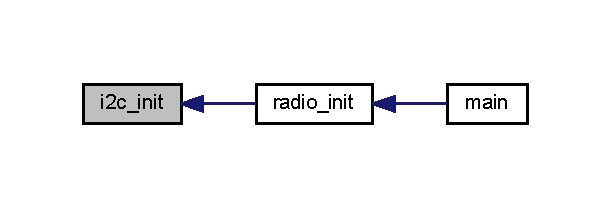
\includegraphics[width=293pt]{i2c_8h_a1ef889b72b844429bc81225d7b6f4f2e_icgraph}
\end{center}
\end{figure}


\hypertarget{i2c_8h_a6dd896b0c82d1aa91a1a8155b41c4566}{}\index{i2c.\+h@{i2c.\+h}!i2c\+\_\+read@{i2c\+\_\+read}}
\index{i2c\+\_\+read@{i2c\+\_\+read}!i2c.\+h@{i2c.\+h}}
\subsubsection[{i2c\+\_\+read}]{\setlength{\rightskip}{0pt plus 5cm}uint8\+\_\+t i2c\+\_\+read (
\begin{DoxyParamCaption}
\item[{uint8\+\_\+t}]{addr, }
\item[{enum {\bf I2\+C\+\_\+\+C\+R\+T\+L\+\_\+\+C\+M\+D}}]{rept\+\_\+start, }
\item[{uint8\+\_\+t}]{Rx\+Bytes, }
\item[{uint8\+\_\+t $\ast$}]{Rx\+Data}
\end{DoxyParamCaption}
)}\label{i2c_8h_a6dd896b0c82d1aa91a1a8155b41c4566}


Receives I2\+C commands until a N\+A\+C\+K is received or received Rx\+Bytes. 


\begin{DoxyParams}{Parameter}
{\em addr} & Slave Address in 7-\/bit format. \\
\hline
{\em rept\+\_\+start} & Command for stop or repeated start. \\
\hline
{\em Rx\+Bytes} & Number of receiving bytes. \\
\hline
{\em $\ast$\+Rx\+Data} & Pointer where received I2\+C commands are be writtn. \\
\hline
\end{DoxyParams}
\begin{DoxyReturn}{Rückgabe}
error 
\end{DoxyReturn}


Definiert in Zeile 138 der Datei i2c.\+c.


\begin{DoxyCode}
139 \{
140     \textcolor{keywordflow}{while}(\hyperlink{i2c_8c_ac88c1666422f322663fc6c63434dba97}{i2c}.\hyperlink{struct_i2_c___c_t_r_l_ade818037fd6c985038ff29656089758d}{status} != \hyperlink{i2c_8h_a8f12d82f4a490ef04de32baf91363d9bafd6a0e4343048b10646dd2976cc5ad18}{IDLE});
141 
142     \textcolor{comment}{/* Set slave address */}
143     UCB0I2CSA = addr;
144 
145     \textcolor{comment}{/* Change pointer to given buffer */}
146     \hyperlink{i2c_8c_ac88c1666422f322663fc6c63434dba97}{i2c}.\hyperlink{struct_i2_c___c_t_r_l_a3c8ed69cf31f6ee7aa513fe5f115ba92}{PRxData} = RxData;
147     \textcolor{comment}{/* Load RX counter */}
148     \hyperlink{i2c_8c_ac88c1666422f322663fc6c63434dba97}{i2c}.\hyperlink{struct_i2_c___c_t_r_l_a37e493c5b47477e45136924079fd9606}{RxByteCtr} = RXBytes;
149 
150     \textcolor{comment}{/* Clear Interrupt */}
151     IE2 = UCB0RXIE;
152 
153     \textcolor{comment}{/* configure receiver mode */}
154     UCB0CTL1 &= ~UCTR;
155 
156     \hyperlink{i2c_8c_ac88c1666422f322663fc6c63434dba97}{i2c}.\hyperlink{struct_i2_c___c_t_r_l_ade818037fd6c985038ff29656089758d}{status} = \hyperlink{i2c_8h_a8f12d82f4a490ef04de32baf91363d9ba563f8ed00490ea22ea2605d9571dada8}{RECEIVE};
157 
158     \textcolor{comment}{/* Send a start condition with read flag */}
159     \textcolor{keywordflow}{if} ( \hyperlink{i2c_8c_ac88c1666422f322663fc6c63434dba97}{i2c}.\hyperlink{struct_i2_c___c_t_r_l_a37e493c5b47477e45136924079fd9606}{RxByteCtr} == 1 ) \{
160         \hyperlink{i2c_8c_ac88c1666422f322663fc6c63434dba97}{i2c}.\hyperlink{struct_i2_c___c_t_r_l_a37e493c5b47477e45136924079fd9606}{RxByteCtr} = 0;
161         \_\_disable\_interrupt();
162         UCB0CTL1 |= UCTXSTT;
163         \textcolor{keywordflow}{while}(UCB0CTL1 & UCTXSTT);
164         UCB0CTL1 |= UCTXSTP;
165         \_\_enable\_interrupt();
166     \}
167     \textcolor{keywordflow}{else} \{
168         \hyperlink{i2c_8c_ac88c1666422f322663fc6c63434dba97}{i2c}.\hyperlink{struct_i2_c___c_t_r_l_a37e493c5b47477e45136924079fd9606}{RxByteCtr} -= 2;
169         UCB0CTL1 |= UCTXSTT;
170     \}
171 
172     \textcolor{keywordflow}{while}(UCB0STAT & UCBBUSY);
173 
174     \hyperlink{i2c_8c_ac88c1666422f322663fc6c63434dba97}{i2c}.\hyperlink{struct_i2_c___c_t_r_l_ade818037fd6c985038ff29656089758d}{status} = \hyperlink{i2c_8h_a8f12d82f4a490ef04de32baf91363d9bafd6a0e4343048b10646dd2976cc5ad18}{IDLE};
175 
176     \textcolor{keywordflow}{return} 0;
177 \}
\end{DoxyCode}


Hier ist ein Graph der zeigt, wo diese Funktion aufgerufen wird\+:
\nopagebreak
\begin{figure}[H]
\begin{center}
\leavevmode
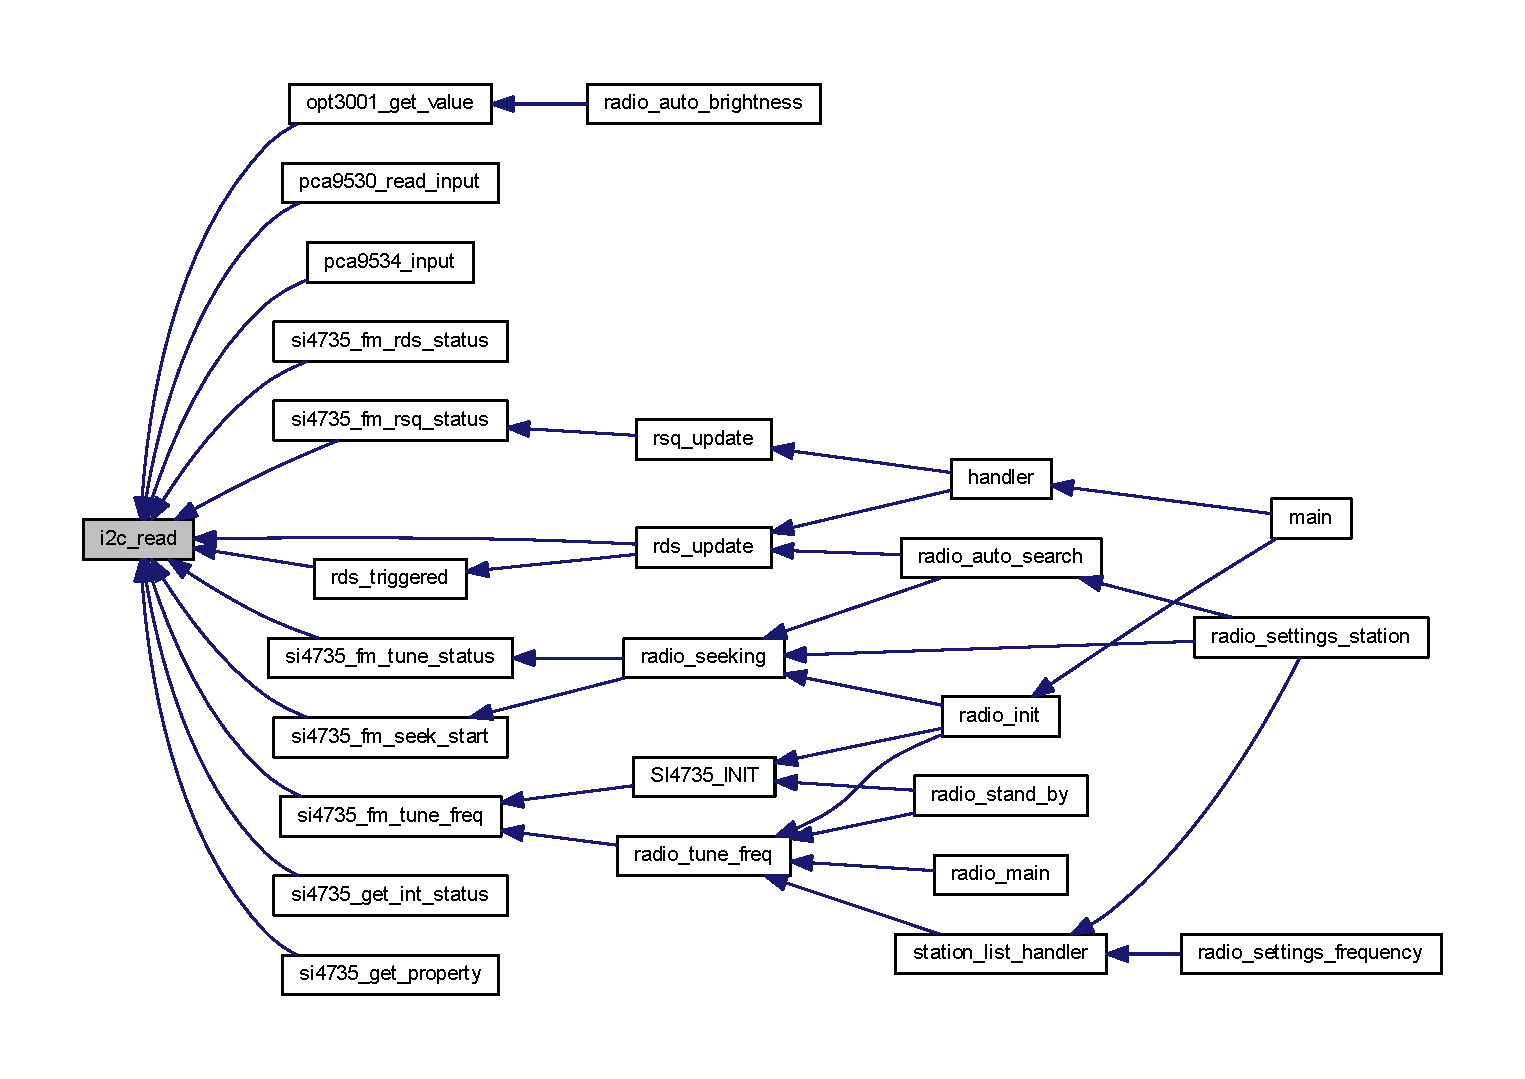
\includegraphics[width=350pt]{i2c_8h_a6dd896b0c82d1aa91a1a8155b41c4566_icgraph}
\end{center}
\end{figure}


\hypertarget{i2c_8h_ae0625b97d3437bcaca4ac4b96dd01978}{}\index{i2c.\+h@{i2c.\+h}!i2c\+\_\+write\+\_\+arr@{i2c\+\_\+write\+\_\+arr}}
\index{i2c\+\_\+write\+\_\+arr@{i2c\+\_\+write\+\_\+arr}!i2c.\+h@{i2c.\+h}}
\subsubsection[{i2c\+\_\+write\+\_\+arr}]{\setlength{\rightskip}{0pt plus 5cm}uint8\+\_\+t i2c\+\_\+write\+\_\+arr (
\begin{DoxyParamCaption}
\item[{uint8\+\_\+t}]{addr, }
\item[{enum {\bf I2\+C\+\_\+\+C\+R\+T\+L\+\_\+\+C\+M\+D}}]{rept\+\_\+start, }
\item[{uint8\+\_\+t}]{n\+\_\+size, }
\item[{uint8\+\_\+t $\ast$}]{Tx\+Data}
\end{DoxyParamCaption}
)}\label{i2c_8h_ae0625b97d3437bcaca4ac4b96dd01978}


Transmits I2\+C command array to a I2\+C slave. 


\begin{DoxyParams}{Parameter}
{\em addr} & Slave Address in 7-\/bit format. \\
\hline
{\em rept\+\_\+start} & Command for stop or repeated start. \\
\hline
{\em n\+\_\+size} & Number of transmitting bytes. \\
\hline
{\em $\ast$\+Tx\+Data} & Pointer to I2\+C command bytes to send. \\
\hline
\end{DoxyParams}
\begin{DoxyReturn}{Rückgabe}
error 
\end{DoxyReturn}


Definiert in Zeile 103 der Datei i2c.\+c.


\begin{DoxyCode}
104 \{
105     \textcolor{comment}{/* Copy pointer from TxData */}
106     \hyperlink{i2c_8c_ac88c1666422f322663fc6c63434dba97}{i2c}.\hyperlink{struct_i2_c___c_t_r_l_af294cab6f89af5bd936b709e202c8421}{PTxData} = TxData;
107 
108     \textcolor{comment}{/* Set slave address */}
109     UCB0I2CSA = addr;
110 
111     \textcolor{comment}{/* Set Transmit Interrupt */}
112     IE2 = UCB0TXIE;
113 
114     \hyperlink{i2c_8c_ac88c1666422f322663fc6c63434dba97}{i2c}.\hyperlink{struct_i2_c___c_t_r_l_a374bcaa6a416b8601564a1053ddf78bb}{rept\_start} = rept\_start;
115 
116     \textcolor{comment}{/* Load TX byte counter */}
117     \hyperlink{i2c_8c_ac88c1666422f322663fc6c63434dba97}{i2c}.\hyperlink{struct_i2_c___c_t_r_l_aec22639ad7dc7eed52b3e116ea3223fe}{TxByteCtr} = n\_size;
118 
119     \hyperlink{i2c_8c_ac88c1666422f322663fc6c63434dba97}{i2c}.\hyperlink{struct_i2_c___c_t_r_l_ade818037fd6c985038ff29656089758d}{status} = \hyperlink{i2c_8h_a8f12d82f4a490ef04de32baf91363d9bad208fa8c08969a9d78096817bf0a6377}{TRANSMIT};
120 
121     \textcolor{comment}{/* Send a start condition with write flag */}
122     UCB0CTL1 |= UCTR + UCTXSTT;
123 
124     \textcolor{comment}{/* Wait until Transmition is complet */}
125     \textcolor{keywordflow}{if}(rept\_start == \hyperlink{i2c_8h_aaaea3962492fd5ad1e43cba027d949d5a679ee5320d66c8322e310daeb2ee99b8}{STOP}) \{
126         \textcolor{keywordflow}{while}(UCB0STAT & UCBBUSY);
127     \}
128     \textcolor{keywordflow}{else} \{
129         \hyperlink{timer_8c_a3c56af3315c2461dec5ced585a5f84db}{\_delay\_ten\_us}(20);
130     \}
131 
132     \hyperlink{i2c_8c_ac88c1666422f322663fc6c63434dba97}{i2c}.\hyperlink{struct_i2_c___c_t_r_l_ade818037fd6c985038ff29656089758d}{status} = \hyperlink{i2c_8h_a8f12d82f4a490ef04de32baf91363d9bafd6a0e4343048b10646dd2976cc5ad18}{IDLE};
133 
134     \textcolor{keywordflow}{return} 0;
135 
136 \}
\end{DoxyCode}


Hier ist ein Graph, der zeigt, was diese Funktion aufruft\+:\nopagebreak
\begin{figure}[H]
\begin{center}
\leavevmode
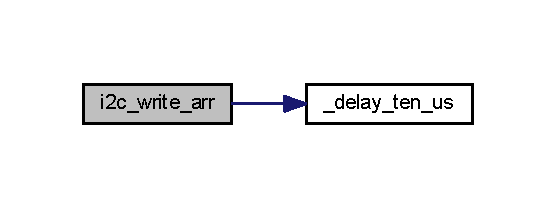
\includegraphics[width=267pt]{i2c_8h_ae0625b97d3437bcaca4ac4b96dd01978_cgraph}
\end{center}
\end{figure}




Hier ist ein Graph der zeigt, wo diese Funktion aufgerufen wird\+:
\nopagebreak
\begin{figure}[H]
\begin{center}
\leavevmode
\includegraphics[width=350pt]{i2c_8h_ae0625b97d3437bcaca4ac4b96dd01978_icgraph}
\end{center}
\end{figure}


\hypertarget{i2c_8h_a6691e5911f539e1e8178c6e983e8079a}{}\index{i2c.\+h@{i2c.\+h}!i2c\+\_\+write\+\_\+var@{i2c\+\_\+write\+\_\+var}}
\index{i2c\+\_\+write\+\_\+var@{i2c\+\_\+write\+\_\+var}!i2c.\+h@{i2c.\+h}}
\subsubsection[{i2c\+\_\+write\+\_\+var}]{\setlength{\rightskip}{0pt plus 5cm}uint8\+\_\+t i2c\+\_\+write\+\_\+var (
\begin{DoxyParamCaption}
\item[{uint8\+\_\+t}]{addr, }
\item[{enum {\bf I2\+C\+\_\+\+C\+R\+T\+L\+\_\+\+C\+M\+D}}]{rept\+\_\+start, }
\item[{uint8\+\_\+t}]{n\+\_\+args, }
\item[{}]{...}
\end{DoxyParamCaption}
)}\label{i2c_8h_a6691e5911f539e1e8178c6e983e8079a}


Transmits I2\+C commands with a variable length to a I2\+C slave. 


\begin{DoxyParams}{Parameter}
{\em addr} & Slave Address in 7-\/bit format. \\
\hline
{\em rept\+\_\+start} & Command for stop or repeated start. \\
\hline
{\em n\+\_\+args} & Number of command bytes. \\
\hline
{\em ...} & I2\+C command bytes to send. \\
\hline
\end{DoxyParams}
\begin{DoxyReturn}{Rückgabe}
error 
\end{DoxyReturn}


Definiert in Zeile 67 der Datei i2c.\+c.


\begin{DoxyCode}
68 \{
69     \textcolor{comment}{/* Wait until all transmitions and receptions done */}
70     \textcolor{keywordflow}{while}( \hyperlink{i2c_8c_ac88c1666422f322663fc6c63434dba97}{i2c}.\hyperlink{struct_i2_c___c_t_r_l_ade818037fd6c985038ff29656089758d}{status} != \hyperlink{i2c_8h_a8f12d82f4a490ef04de32baf91363d9bafd6a0e4343048b10646dd2976cc5ad18}{IDLE});
71 
72 \textcolor{preprocessor}{#if VARIADIC\_IMPLEMENTATION}
73 
74     \textcolor{comment}{/* Reserve size of memory for transmit buffer if buffer is uninitialised*/}
75     \textcolor{keywordflow}{if}(\hyperlink{i2c_8c_ac20eea448283bc60729067c96d439ae8}{PTxData} == 0) \{
76         \hyperlink{i2c_8c_ac20eea448283bc60729067c96d439ae8}{PTxData} = (uint8\_t *) malloc(n\_args * \textcolor{keyword}{sizeof}(uint8\_t));
77         \hyperlink{i2c_8c_ac88c1666422f322663fc6c63434dba97}{i2c}.\hyperlink{struct_i2_c___c_t_r_l_a28b787f8db17314755d031d75ec38017}{TxByteRes} = n\_args;
78     \}
79     \textcolor{comment}{/* Reserve more memory if actual size not enough */}
80     \textcolor{keywordflow}{else} \{
81         \textcolor{keywordflow}{if}(\hyperlink{i2c_8c_ac88c1666422f322663fc6c63434dba97}{i2c}.\hyperlink{struct_i2_c___c_t_r_l_a28b787f8db17314755d031d75ec38017}{TxByteRes} < n\_args) \{
82             \hyperlink{i2c_8c_ac20eea448283bc60729067c96d439ae8}{PTxData} = (uint8\_t *) realloc(\hyperlink{i2c_8c_ac20eea448283bc60729067c96d439ae8}{PTxData}, n\_args * \textcolor{keyword}{sizeof}(uint8\_t));
83             \hyperlink{i2c_8c_ac88c1666422f322663fc6c63434dba97}{i2c}.\hyperlink{struct_i2_c___c_t_r_l_a28b787f8db17314755d031d75ec38017}{TxByteRes} = n\_args;
84         \}
85     \}
86 
87 \textcolor{preprocessor}{#endif }\textcolor{comment}{/* VARIADIC\_IMPLEMENTATION */}\textcolor{preprocessor}{}
88 
89     uint8\_t i = 0;
90     va\_list ap;
91 
92     \textcolor{comment}{/* Read n\_args from function}
93 \textcolor{comment}{     * Copy args to transmit buffer}
94 \textcolor{comment}{     */}
95     va\_start(ap, n\_args);
96     \textcolor{keywordflow}{for}(i = 0; i < n\_args; i++)
97         \hyperlink{i2c_8c_ac20eea448283bc60729067c96d439ae8}{PTxData}[i] = va\_arg(ap, uint8\_t);
98     va\_end(ap);
99 
100     \textcolor{keywordflow}{return} \hyperlink{i2c_8c_ae0625b97d3437bcaca4ac4b96dd01978}{i2c\_write\_arr}(addr, rept\_start, n\_args, \hyperlink{i2c_8c_ac20eea448283bc60729067c96d439ae8}{PTxData});
101 \}
\end{DoxyCode}


Hier ist ein Graph, der zeigt, was diese Funktion aufruft\+:\nopagebreak
\begin{figure}[H]
\begin{center}
\leavevmode
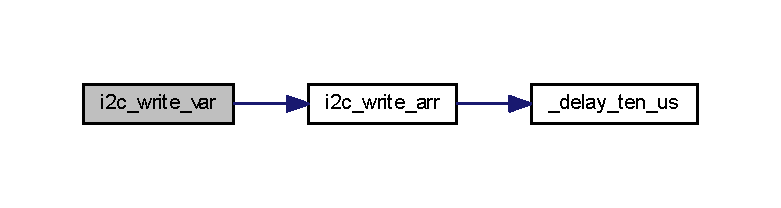
\includegraphics[width=350pt]{i2c_8h_a6691e5911f539e1e8178c6e983e8079a_cgraph}
\end{center}
\end{figure}




Hier ist ein Graph der zeigt, wo diese Funktion aufgerufen wird\+:
\nopagebreak
\begin{figure}[H]
\begin{center}
\leavevmode
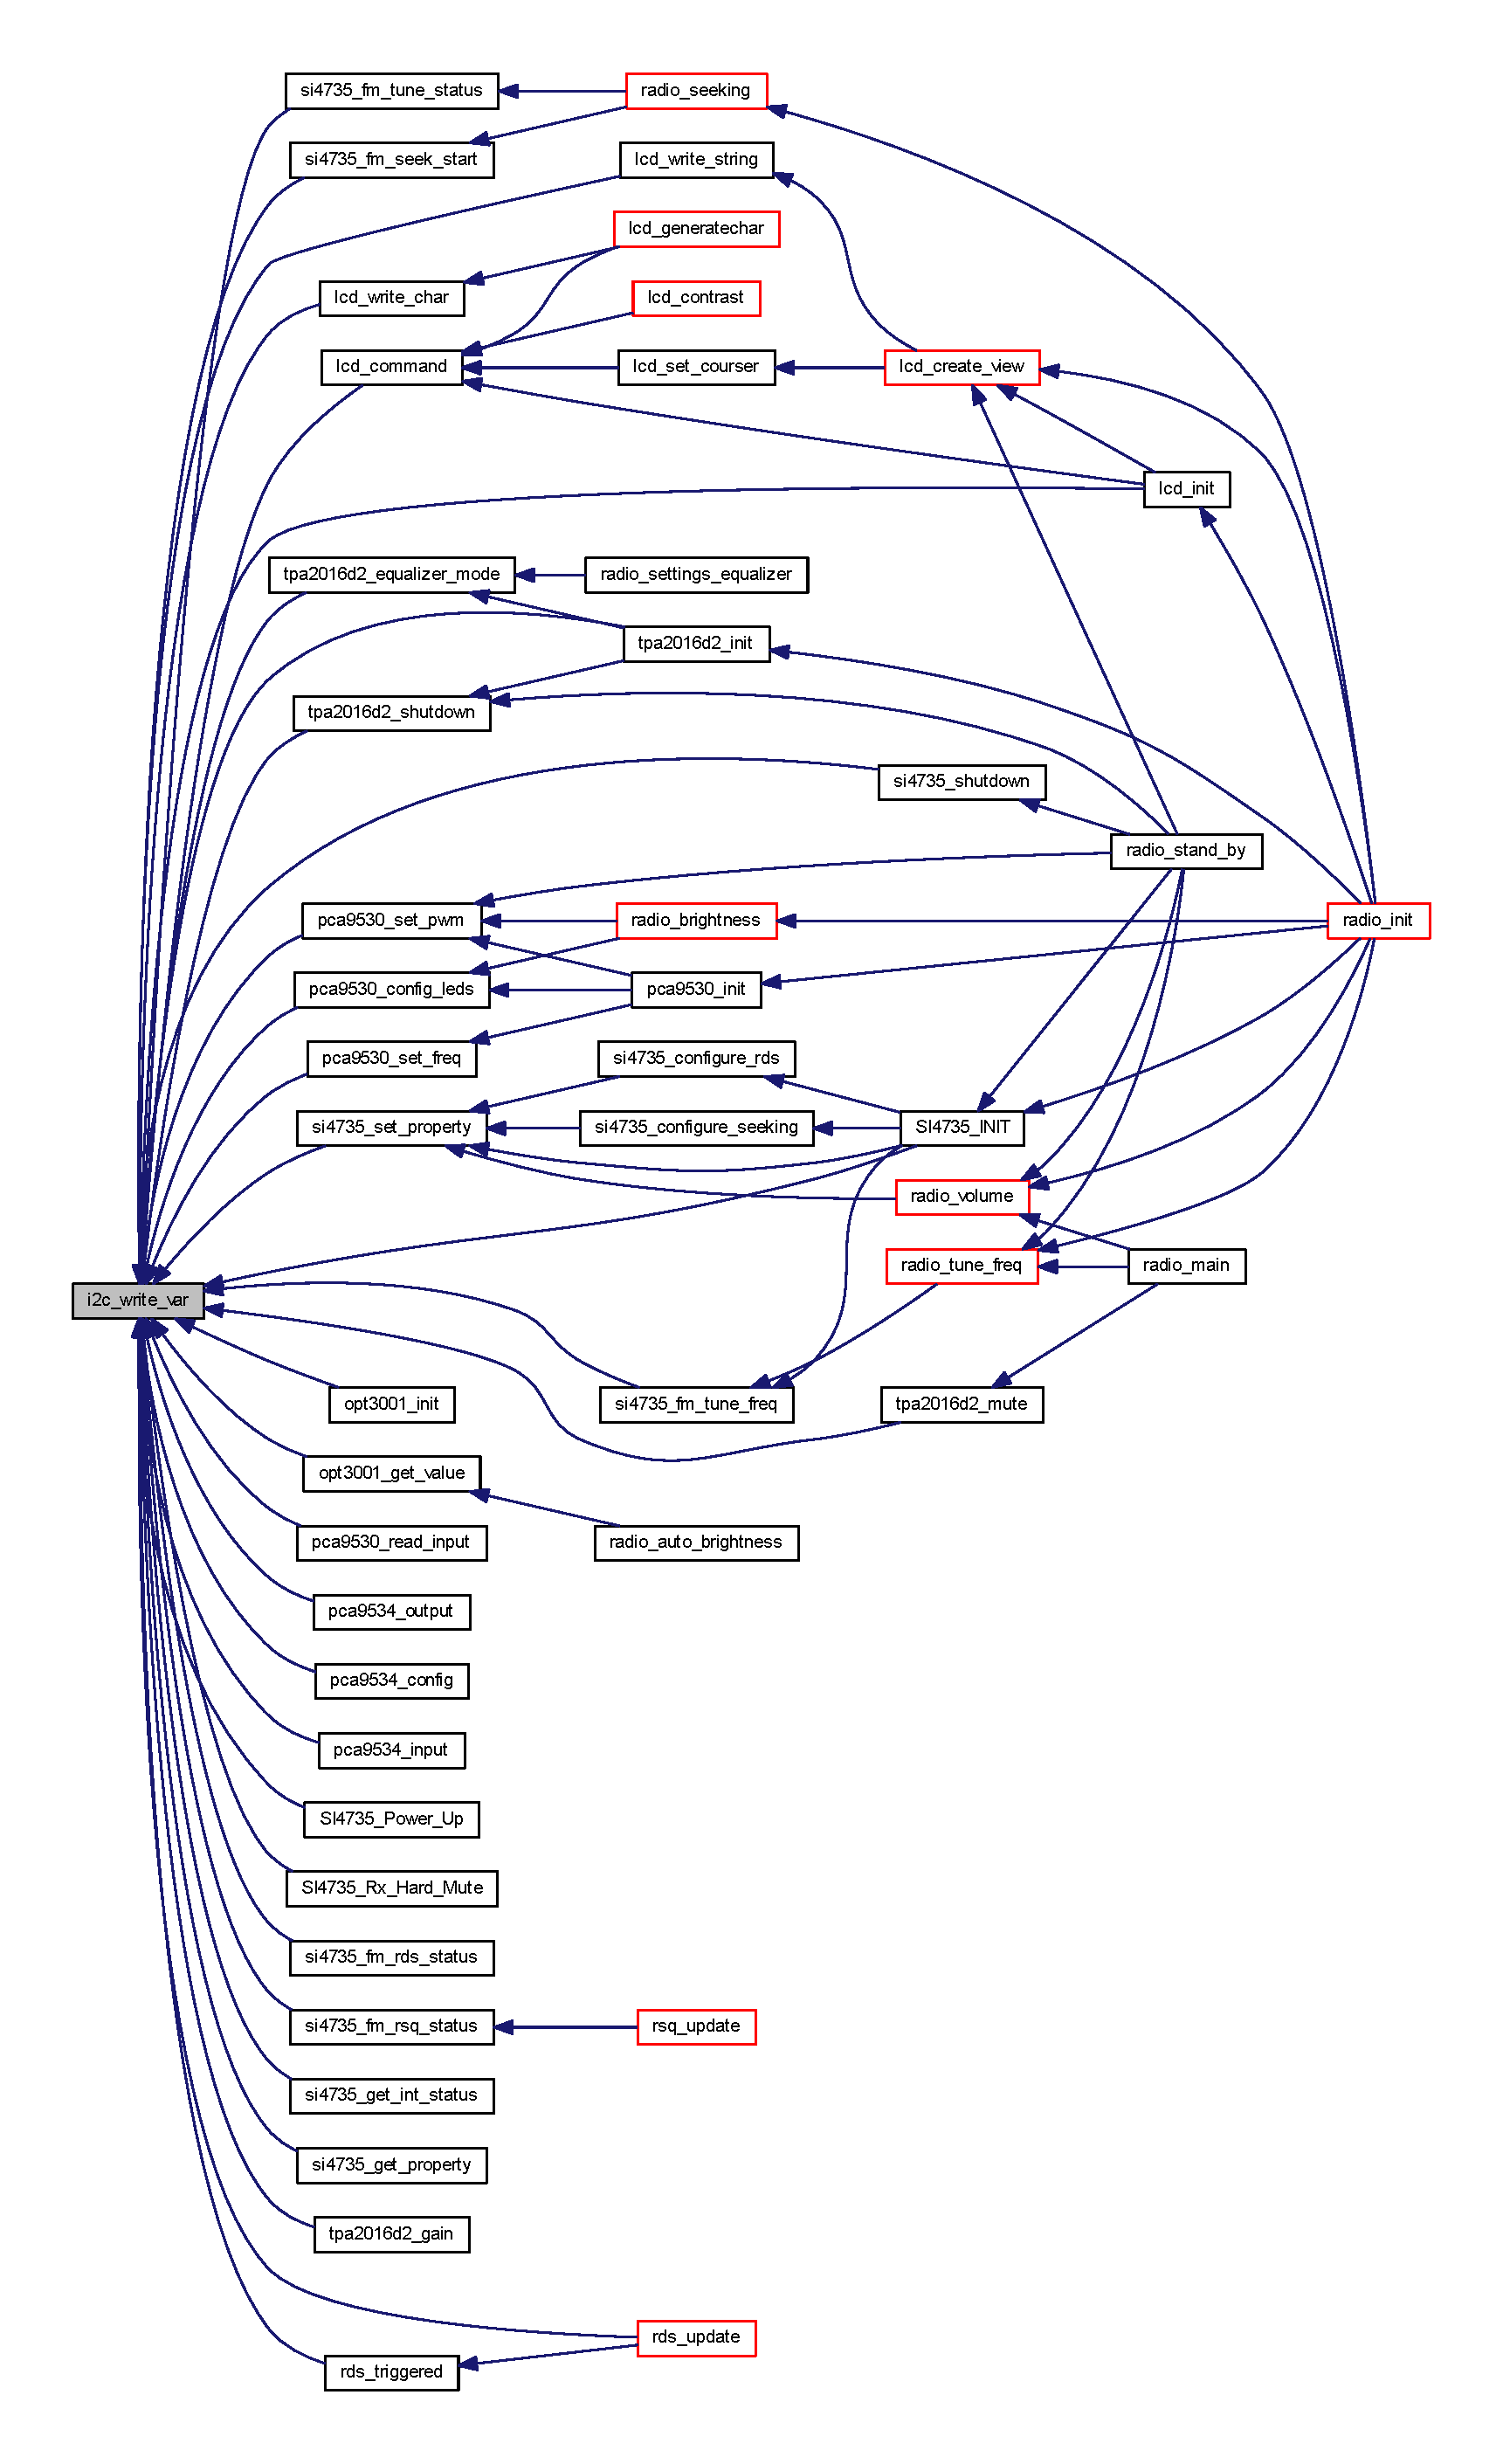
\includegraphics[height=550pt]{i2c_8h_a6691e5911f539e1e8178c6e983e8079a_icgraph}
\end{center}
\end{figure}



\hypertarget{lcd__commands_8h}{}\section{D\+:/\+G\+I\+T/fhradiov2/driver/include/lcd\+\_\+commands.h-\/\+Dateireferenz}
\label{lcd__commands_8h}\index{D\+:/\+G\+I\+T/fhradiov2/driver/include/lcd\+\_\+commands.\+h@{D\+:/\+G\+I\+T/fhradiov2/driver/include/lcd\+\_\+commands.\+h}}
Dieser Graph zeigt, welche Datei direkt oder indirekt diese Datei enthält\+:
\nopagebreak
\begin{figure}[H]
\begin{center}
\leavevmode
\includegraphics[width=350pt]{lcd__commands_8h__dep__incl}
\end{center}
\end{figure}
\subsection*{Makrodefinitionen}
\begin{DoxyCompactItemize}
\item 
\#define \hyperlink{lcd__commands_8h_a8ab3108396a0d33dbf7f3ab6477ba01d}{L\+C\+D\+\_\+\+S\+H\+I\+F\+T\+\_\+\+R\+I\+G\+H\+T}~0x1\+C
\item 
\#define \hyperlink{lcd__commands_8h_a941377571f34b9d898b61ce89f10226d}{L\+C\+D\+\_\+\+S\+H\+I\+F\+T\+\_\+\+L\+E\+F\+T}~0x18
\item 
\#define \hyperlink{lcd__commands_8h_a350fda109811fb23bfaf6ef763c31b9b}{L\+C\+D\+\_\+\+R\+E\+S\+E\+T\+\_\+\+C\+O\+U\+R\+S\+E\+R}~0x02
\item 
\#define \hyperlink{lcd__commands_8h_ad3c37e4453c7f7ba2d5220f9d8fa8502}{L\+C\+D\+\_\+\+A\+D\+R\+E\+S\+S\+\_\+\+L\+I\+N\+E\+\_\+1}~0x80
\item 
\#define \hyperlink{lcd__commands_8h_a357f0824fb224d0925d6ca5230585814}{L\+C\+D\+\_\+\+A\+D\+R\+E\+S\+S\+\_\+\+L\+I\+N\+E\+\_\+2}~0x90
\item 
\#define \hyperlink{lcd__commands_8h_a0531c4c867eea2495519880aecd7c422}{L\+C\+D\+\_\+\+A\+D\+R\+E\+S\+S\+\_\+\+L\+I\+N\+E\+\_\+3}~0x\+A0
\item 
\#define \hyperlink{lcd__commands_8h_a467510be8265e0cc87ce3e4110f9e75e}{L\+C\+D\+\_\+\+A\+D\+R\+E\+S\+S\+\_\+\+L\+I\+N\+E\+\_\+4}~0x\+D4
\item 
\#define \hyperlink{lcd__commands_8h_ac547b969070db1798702062faca30c6e}{L\+C\+D\+\_\+\+C\+L\+E\+A\+R\+\_\+\+S\+C\+R\+E\+E\+N}~0x01
\item 
\#define \hyperlink{lcd__commands_8h_ae5e77a91b0fef0c36af29424a1ee2da1}{L\+C\+D\+\_\+\+E\+N\+T\+R\+Y\+\_\+\+M\+O\+D\+E\+\_\+\+S\+E\+T}~0x04
\item 
\#define \hyperlink{lcd__commands_8h_a6e5a50c1f9f21c012e6d44ebcd5fd65f}{L\+C\+D\+\_\+\+C\+O\+U\+R\+S\+E\+R\+\_\+\+I\+N\+K\+R\+E\+M\+E\+N\+T}~0x02
\item 
\#define \hyperlink{lcd__commands_8h_aab6f7a7ed8d25f1d06060e34a77a78f0}{L\+C\+D\+\_\+\+D\+I\+S\+P\+L\+A\+Y\+\_\+\+C\+O\+N\+T\+E\+\_\+\+M\+O\+V\+E}~0x01
\item 
\#define \hyperlink{lcd__commands_8h_a9b4eda8a777de7cc4b7cbaa71621029e}{L\+C\+D\+\_\+\+D\+I\+S\+P\+L\+A\+Y\+\_\+\+C\+O\+N\+T\+R\+O\+L}~0x08
\item 
\#define \hyperlink{lcd__commands_8h_a846dac5d1bb72bef7a76ee110c0445b6}{L\+C\+D\+\_\+\+D\+I\+S\+P\+L\+A\+Y\+\_\+\+O\+N}~0x04
\item 
\#define \hyperlink{lcd__commands_8h_a4c627e9b4e139cb5ebab107c3087df7a}{L\+C\+D\+\_\+\+C\+O\+U\+R\+S\+E\+R\+\_\+\+O\+N}~0x02
\item 
\#define \hyperlink{lcd__commands_8h_a45d3a5576d1002ead2fb4d9a813f2538}{L\+C\+D\+\_\+\+C\+O\+U\+R\+S\+E\+R\+\_\+\+B\+L\+I\+N\+K}~0x01
\item 
\#define \hyperlink{lcd__commands_8h_af8ec7e043a3b67ee423b97783d08aeb1}{L\+C\+D\+\_\+\+F\+U\+N\+C\+T\+I\+O\+N\+\_\+\+S\+E\+T}~0x20
\item 
\#define \hyperlink{lcd__commands_8h_a028e7ea27d1e98ccc598c09a8184ba08}{L\+C\+D\+\_\+8\+B\+T\+I\+\_\+\+M\+O\+D\+E}~0x10
\item 
\#define \hyperlink{lcd__commands_8h_a8158610f55224e1cbb4b495e38d4b951}{L\+C\+D\+\_\+5x10\+\_\+\+F\+O\+N\+T}~0x04
\item 
\#define \hyperlink{lcd__commands_8h_add84145ade06b4f96934b7f1ed712e50}{L\+C\+D\+\_\+2\+\_\+\+L\+I\+N\+E\+\_\+\+I\+N\+S\+T\+\_\+1}~0x09
\item 
\#define \hyperlink{lcd__commands_8h_a77febe1793148d377a47feafd8f00f2a}{L\+C\+D\+\_\+\+I\+N\+S\+T\+\_\+0}~0x08
\item 
\#define \hyperlink{lcd__commands_8h_a5109f670d7f397ba8845d08167bf4ab2}{L\+C\+D\+\_\+\+S\+E\+T\+\_\+\+C\+G\+A\+D\+R}~0x40
\item 
\#define \hyperlink{lcd__commands_8h_aa16d1fe8c9651f81c3f1649e57bc870c}{L\+C\+D\+\_\+\+B\+I\+A\+S\+\_\+\+S\+E\+T}~0x14
\item 
\#define \hyperlink{lcd__commands_8h_a3e0a4be625c4ed54cf0257a3b526ea00}{L\+C\+D\+\_\+\+B\+I\+A\+S\+\_\+1\+\_\+4}~0x08
\item 
\#define \hyperlink{lcd__commands_8h_af685b6108573c92216437b1a512c6a72}{L\+C\+D\+\_\+3\+\_\+\+L\+I\+N\+E}~0x01
\item 
\#define \hyperlink{lcd__commands_8h_a09afb8c9876350b83530222841b6b4ca}{L\+C\+D\+\_\+\+P\+O\+W\+E\+R\+\_\+\+C\+O\+N\+T\+R\+O\+L}~0x50
\item 
\#define \hyperlink{lcd__commands_8h_a6fd38eab7f42a02c3ab53b1470a8cd87}{L\+C\+D\+\_\+\+I\+C\+O\+N\+\_\+\+O\+N}~0x08
\item 
\#define \hyperlink{lcd__commands_8h_a18dee2878389a58570c4a5d15eec6562}{L\+C\+D\+\_\+\+B\+O\+O\+S\+T\+E\+R\+\_\+\+O\+N}~0x04
\item 
\#define \hyperlink{lcd__commands_8h_a73c8e3c5079066c54f1f873efb5eda6a}{L\+C\+D\+\_\+\+C\+O\+N\+T\+R\+A\+S\+T\+\_\+1}~0x00
\item 
\#define \hyperlink{lcd__commands_8h_aa182b257140f187c7ceb85761802a6d4}{L\+C\+D\+\_\+\+F\+O\+L\+L\+O\+W\+E\+R\+\_\+\+C\+O\+N\+T\+R\+O\+L}~0x60
\item 
\#define \hyperlink{lcd__commands_8h_aa7170591c5c6954165b8f1b6c94bdcea}{L\+C\+D\+\_\+\+F\+O\+L\+L\+O\+W\+E\+R\+\_\+\+C\+I\+R\+C\+U\+T\+\_\+\+O\+N}~0x08
\item 
\#define \hyperlink{lcd__commands_8h_af05126b3001c839af73fdbc7e2b0940e}{L\+C\+D\+\_\+\+A\+M\+P\+L\+I\+F\+F\+E\+D\+\_\+\+R\+A\+T\+I\+O}~0x04
\item 
\#define \hyperlink{lcd__commands_8h_a2dc0a014e84d69016cc4785bbc1fb3ac}{L\+C\+D\+\_\+\+C\+O\+N\+T\+R\+A\+S\+T\+\_\+\+S\+E\+T}~0x70
\item 
\#define \hyperlink{lcd__commands_8h_a59e3a59c04e3767a917635367d5c1c05}{L\+C\+D\+\_\+\+C\+O\+N\+T\+R\+A\+S\+T\+\_\+2}~0x0\+C
\item 
\#define \hyperlink{lcd__commands_8h_afb9a52fe082bc759811cbc78af93e5be}{L\+C\+D\+\_\+\+L\+O\+W\+E\+R\+\_\+\+B\+Y\+T\+E}(byte)~(byte \& 0x0f)
\item 
\#define \hyperlink{lcd__commands_8h_afd4bb10e8cc3368a80abe3ef75d92c39}{L\+C\+D\+\_\+\+H\+I\+G\+H\+E\+R\+\_\+\+B\+Y\+T\+E}(byte)~((byte$>$$>$4) \& 0x0f)
\end{DoxyCompactItemize}


\subsection{Makro-\/\+Dokumentation}
\hypertarget{lcd__commands_8h_add84145ade06b4f96934b7f1ed712e50}{}\index{lcd\+\_\+commands.\+h@{lcd\+\_\+commands.\+h}!L\+C\+D\+\_\+2\+\_\+\+L\+I\+N\+E\+\_\+\+I\+N\+S\+T\+\_\+1@{L\+C\+D\+\_\+2\+\_\+\+L\+I\+N\+E\+\_\+\+I\+N\+S\+T\+\_\+1}}
\index{L\+C\+D\+\_\+2\+\_\+\+L\+I\+N\+E\+\_\+\+I\+N\+S\+T\+\_\+1@{L\+C\+D\+\_\+2\+\_\+\+L\+I\+N\+E\+\_\+\+I\+N\+S\+T\+\_\+1}!lcd\+\_\+commands.\+h@{lcd\+\_\+commands.\+h}}
\subsubsection[{L\+C\+D\+\_\+2\+\_\+\+L\+I\+N\+E\+\_\+\+I\+N\+S\+T\+\_\+1}]{\setlength{\rightskip}{0pt plus 5cm}\#define L\+C\+D\+\_\+2\+\_\+\+L\+I\+N\+E\+\_\+\+I\+N\+S\+T\+\_\+1~0x09}\label{lcd__commands_8h_add84145ade06b4f96934b7f1ed712e50}


Definiert in Zeile 29 der Datei lcd\+\_\+commands.\+h.

\hypertarget{lcd__commands_8h_af685b6108573c92216437b1a512c6a72}{}\index{lcd\+\_\+commands.\+h@{lcd\+\_\+commands.\+h}!L\+C\+D\+\_\+3\+\_\+\+L\+I\+N\+E@{L\+C\+D\+\_\+3\+\_\+\+L\+I\+N\+E}}
\index{L\+C\+D\+\_\+3\+\_\+\+L\+I\+N\+E@{L\+C\+D\+\_\+3\+\_\+\+L\+I\+N\+E}!lcd\+\_\+commands.\+h@{lcd\+\_\+commands.\+h}}
\subsubsection[{L\+C\+D\+\_\+3\+\_\+\+L\+I\+N\+E}]{\setlength{\rightskip}{0pt plus 5cm}\#define L\+C\+D\+\_\+3\+\_\+\+L\+I\+N\+E~0x01}\label{lcd__commands_8h_af685b6108573c92216437b1a512c6a72}


Definiert in Zeile 34 der Datei lcd\+\_\+commands.\+h.

\hypertarget{lcd__commands_8h_a8158610f55224e1cbb4b495e38d4b951}{}\index{lcd\+\_\+commands.\+h@{lcd\+\_\+commands.\+h}!L\+C\+D\+\_\+5x10\+\_\+\+F\+O\+N\+T@{L\+C\+D\+\_\+5x10\+\_\+\+F\+O\+N\+T}}
\index{L\+C\+D\+\_\+5x10\+\_\+\+F\+O\+N\+T@{L\+C\+D\+\_\+5x10\+\_\+\+F\+O\+N\+T}!lcd\+\_\+commands.\+h@{lcd\+\_\+commands.\+h}}
\subsubsection[{L\+C\+D\+\_\+5x10\+\_\+\+F\+O\+N\+T}]{\setlength{\rightskip}{0pt plus 5cm}\#define L\+C\+D\+\_\+5x10\+\_\+\+F\+O\+N\+T~0x04}\label{lcd__commands_8h_a8158610f55224e1cbb4b495e38d4b951}


Definiert in Zeile 28 der Datei lcd\+\_\+commands.\+h.

\hypertarget{lcd__commands_8h_a028e7ea27d1e98ccc598c09a8184ba08}{}\index{lcd\+\_\+commands.\+h@{lcd\+\_\+commands.\+h}!L\+C\+D\+\_\+8\+B\+T\+I\+\_\+\+M\+O\+D\+E@{L\+C\+D\+\_\+8\+B\+T\+I\+\_\+\+M\+O\+D\+E}}
\index{L\+C\+D\+\_\+8\+B\+T\+I\+\_\+\+M\+O\+D\+E@{L\+C\+D\+\_\+8\+B\+T\+I\+\_\+\+M\+O\+D\+E}!lcd\+\_\+commands.\+h@{lcd\+\_\+commands.\+h}}
\subsubsection[{L\+C\+D\+\_\+8\+B\+T\+I\+\_\+\+M\+O\+D\+E}]{\setlength{\rightskip}{0pt plus 5cm}\#define L\+C\+D\+\_\+8\+B\+T\+I\+\_\+\+M\+O\+D\+E~0x10}\label{lcd__commands_8h_a028e7ea27d1e98ccc598c09a8184ba08}


Definiert in Zeile 27 der Datei lcd\+\_\+commands.\+h.

\hypertarget{lcd__commands_8h_ad3c37e4453c7f7ba2d5220f9d8fa8502}{}\index{lcd\+\_\+commands.\+h@{lcd\+\_\+commands.\+h}!L\+C\+D\+\_\+\+A\+D\+R\+E\+S\+S\+\_\+\+L\+I\+N\+E\+\_\+1@{L\+C\+D\+\_\+\+A\+D\+R\+E\+S\+S\+\_\+\+L\+I\+N\+E\+\_\+1}}
\index{L\+C\+D\+\_\+\+A\+D\+R\+E\+S\+S\+\_\+\+L\+I\+N\+E\+\_\+1@{L\+C\+D\+\_\+\+A\+D\+R\+E\+S\+S\+\_\+\+L\+I\+N\+E\+\_\+1}!lcd\+\_\+commands.\+h@{lcd\+\_\+commands.\+h}}
\subsubsection[{L\+C\+D\+\_\+\+A\+D\+R\+E\+S\+S\+\_\+\+L\+I\+N\+E\+\_\+1}]{\setlength{\rightskip}{0pt plus 5cm}\#define L\+C\+D\+\_\+\+A\+D\+R\+E\+S\+S\+\_\+\+L\+I\+N\+E\+\_\+1~0x80}\label{lcd__commands_8h_ad3c37e4453c7f7ba2d5220f9d8fa8502}


Definiert in Zeile 14 der Datei lcd\+\_\+commands.\+h.

\hypertarget{lcd__commands_8h_a357f0824fb224d0925d6ca5230585814}{}\index{lcd\+\_\+commands.\+h@{lcd\+\_\+commands.\+h}!L\+C\+D\+\_\+\+A\+D\+R\+E\+S\+S\+\_\+\+L\+I\+N\+E\+\_\+2@{L\+C\+D\+\_\+\+A\+D\+R\+E\+S\+S\+\_\+\+L\+I\+N\+E\+\_\+2}}
\index{L\+C\+D\+\_\+\+A\+D\+R\+E\+S\+S\+\_\+\+L\+I\+N\+E\+\_\+2@{L\+C\+D\+\_\+\+A\+D\+R\+E\+S\+S\+\_\+\+L\+I\+N\+E\+\_\+2}!lcd\+\_\+commands.\+h@{lcd\+\_\+commands.\+h}}
\subsubsection[{L\+C\+D\+\_\+\+A\+D\+R\+E\+S\+S\+\_\+\+L\+I\+N\+E\+\_\+2}]{\setlength{\rightskip}{0pt plus 5cm}\#define L\+C\+D\+\_\+\+A\+D\+R\+E\+S\+S\+\_\+\+L\+I\+N\+E\+\_\+2~0x90}\label{lcd__commands_8h_a357f0824fb224d0925d6ca5230585814}


Definiert in Zeile 15 der Datei lcd\+\_\+commands.\+h.

\hypertarget{lcd__commands_8h_a0531c4c867eea2495519880aecd7c422}{}\index{lcd\+\_\+commands.\+h@{lcd\+\_\+commands.\+h}!L\+C\+D\+\_\+\+A\+D\+R\+E\+S\+S\+\_\+\+L\+I\+N\+E\+\_\+3@{L\+C\+D\+\_\+\+A\+D\+R\+E\+S\+S\+\_\+\+L\+I\+N\+E\+\_\+3}}
\index{L\+C\+D\+\_\+\+A\+D\+R\+E\+S\+S\+\_\+\+L\+I\+N\+E\+\_\+3@{L\+C\+D\+\_\+\+A\+D\+R\+E\+S\+S\+\_\+\+L\+I\+N\+E\+\_\+3}!lcd\+\_\+commands.\+h@{lcd\+\_\+commands.\+h}}
\subsubsection[{L\+C\+D\+\_\+\+A\+D\+R\+E\+S\+S\+\_\+\+L\+I\+N\+E\+\_\+3}]{\setlength{\rightskip}{0pt plus 5cm}\#define L\+C\+D\+\_\+\+A\+D\+R\+E\+S\+S\+\_\+\+L\+I\+N\+E\+\_\+3~0x\+A0}\label{lcd__commands_8h_a0531c4c867eea2495519880aecd7c422}


Definiert in Zeile 16 der Datei lcd\+\_\+commands.\+h.

\hypertarget{lcd__commands_8h_a467510be8265e0cc87ce3e4110f9e75e}{}\index{lcd\+\_\+commands.\+h@{lcd\+\_\+commands.\+h}!L\+C\+D\+\_\+\+A\+D\+R\+E\+S\+S\+\_\+\+L\+I\+N\+E\+\_\+4@{L\+C\+D\+\_\+\+A\+D\+R\+E\+S\+S\+\_\+\+L\+I\+N\+E\+\_\+4}}
\index{L\+C\+D\+\_\+\+A\+D\+R\+E\+S\+S\+\_\+\+L\+I\+N\+E\+\_\+4@{L\+C\+D\+\_\+\+A\+D\+R\+E\+S\+S\+\_\+\+L\+I\+N\+E\+\_\+4}!lcd\+\_\+commands.\+h@{lcd\+\_\+commands.\+h}}
\subsubsection[{L\+C\+D\+\_\+\+A\+D\+R\+E\+S\+S\+\_\+\+L\+I\+N\+E\+\_\+4}]{\setlength{\rightskip}{0pt plus 5cm}\#define L\+C\+D\+\_\+\+A\+D\+R\+E\+S\+S\+\_\+\+L\+I\+N\+E\+\_\+4~0x\+D4}\label{lcd__commands_8h_a467510be8265e0cc87ce3e4110f9e75e}


Definiert in Zeile 17 der Datei lcd\+\_\+commands.\+h.

\hypertarget{lcd__commands_8h_af05126b3001c839af73fdbc7e2b0940e}{}\index{lcd\+\_\+commands.\+h@{lcd\+\_\+commands.\+h}!L\+C\+D\+\_\+\+A\+M\+P\+L\+I\+F\+F\+E\+D\+\_\+\+R\+A\+T\+I\+O@{L\+C\+D\+\_\+\+A\+M\+P\+L\+I\+F\+F\+E\+D\+\_\+\+R\+A\+T\+I\+O}}
\index{L\+C\+D\+\_\+\+A\+M\+P\+L\+I\+F\+F\+E\+D\+\_\+\+R\+A\+T\+I\+O@{L\+C\+D\+\_\+\+A\+M\+P\+L\+I\+F\+F\+E\+D\+\_\+\+R\+A\+T\+I\+O}!lcd\+\_\+commands.\+h@{lcd\+\_\+commands.\+h}}
\subsubsection[{L\+C\+D\+\_\+\+A\+M\+P\+L\+I\+F\+F\+E\+D\+\_\+\+R\+A\+T\+I\+O}]{\setlength{\rightskip}{0pt plus 5cm}\#define L\+C\+D\+\_\+\+A\+M\+P\+L\+I\+F\+F\+E\+D\+\_\+\+R\+A\+T\+I\+O~0x04}\label{lcd__commands_8h_af05126b3001c839af73fdbc7e2b0940e}


Definiert in Zeile 41 der Datei lcd\+\_\+commands.\+h.

\hypertarget{lcd__commands_8h_a3e0a4be625c4ed54cf0257a3b526ea00}{}\index{lcd\+\_\+commands.\+h@{lcd\+\_\+commands.\+h}!L\+C\+D\+\_\+\+B\+I\+A\+S\+\_\+1\+\_\+4@{L\+C\+D\+\_\+\+B\+I\+A\+S\+\_\+1\+\_\+4}}
\index{L\+C\+D\+\_\+\+B\+I\+A\+S\+\_\+1\+\_\+4@{L\+C\+D\+\_\+\+B\+I\+A\+S\+\_\+1\+\_\+4}!lcd\+\_\+commands.\+h@{lcd\+\_\+commands.\+h}}
\subsubsection[{L\+C\+D\+\_\+\+B\+I\+A\+S\+\_\+1\+\_\+4}]{\setlength{\rightskip}{0pt plus 5cm}\#define L\+C\+D\+\_\+\+B\+I\+A\+S\+\_\+1\+\_\+4~0x08}\label{lcd__commands_8h_a3e0a4be625c4ed54cf0257a3b526ea00}


Definiert in Zeile 33 der Datei lcd\+\_\+commands.\+h.

\hypertarget{lcd__commands_8h_aa16d1fe8c9651f81c3f1649e57bc870c}{}\index{lcd\+\_\+commands.\+h@{lcd\+\_\+commands.\+h}!L\+C\+D\+\_\+\+B\+I\+A\+S\+\_\+\+S\+E\+T@{L\+C\+D\+\_\+\+B\+I\+A\+S\+\_\+\+S\+E\+T}}
\index{L\+C\+D\+\_\+\+B\+I\+A\+S\+\_\+\+S\+E\+T@{L\+C\+D\+\_\+\+B\+I\+A\+S\+\_\+\+S\+E\+T}!lcd\+\_\+commands.\+h@{lcd\+\_\+commands.\+h}}
\subsubsection[{L\+C\+D\+\_\+\+B\+I\+A\+S\+\_\+\+S\+E\+T}]{\setlength{\rightskip}{0pt plus 5cm}\#define L\+C\+D\+\_\+\+B\+I\+A\+S\+\_\+\+S\+E\+T~0x14}\label{lcd__commands_8h_aa16d1fe8c9651f81c3f1649e57bc870c}


Definiert in Zeile 32 der Datei lcd\+\_\+commands.\+h.

\hypertarget{lcd__commands_8h_a18dee2878389a58570c4a5d15eec6562}{}\index{lcd\+\_\+commands.\+h@{lcd\+\_\+commands.\+h}!L\+C\+D\+\_\+\+B\+O\+O\+S\+T\+E\+R\+\_\+\+O\+N@{L\+C\+D\+\_\+\+B\+O\+O\+S\+T\+E\+R\+\_\+\+O\+N}}
\index{L\+C\+D\+\_\+\+B\+O\+O\+S\+T\+E\+R\+\_\+\+O\+N@{L\+C\+D\+\_\+\+B\+O\+O\+S\+T\+E\+R\+\_\+\+O\+N}!lcd\+\_\+commands.\+h@{lcd\+\_\+commands.\+h}}
\subsubsection[{L\+C\+D\+\_\+\+B\+O\+O\+S\+T\+E\+R\+\_\+\+O\+N}]{\setlength{\rightskip}{0pt plus 5cm}\#define L\+C\+D\+\_\+\+B\+O\+O\+S\+T\+E\+R\+\_\+\+O\+N~0x04}\label{lcd__commands_8h_a18dee2878389a58570c4a5d15eec6562}


Definiert in Zeile 37 der Datei lcd\+\_\+commands.\+h.

\hypertarget{lcd__commands_8h_ac547b969070db1798702062faca30c6e}{}\index{lcd\+\_\+commands.\+h@{lcd\+\_\+commands.\+h}!L\+C\+D\+\_\+\+C\+L\+E\+A\+R\+\_\+\+S\+C\+R\+E\+E\+N@{L\+C\+D\+\_\+\+C\+L\+E\+A\+R\+\_\+\+S\+C\+R\+E\+E\+N}}
\index{L\+C\+D\+\_\+\+C\+L\+E\+A\+R\+\_\+\+S\+C\+R\+E\+E\+N@{L\+C\+D\+\_\+\+C\+L\+E\+A\+R\+\_\+\+S\+C\+R\+E\+E\+N}!lcd\+\_\+commands.\+h@{lcd\+\_\+commands.\+h}}
\subsubsection[{L\+C\+D\+\_\+\+C\+L\+E\+A\+R\+\_\+\+S\+C\+R\+E\+E\+N}]{\setlength{\rightskip}{0pt plus 5cm}\#define L\+C\+D\+\_\+\+C\+L\+E\+A\+R\+\_\+\+S\+C\+R\+E\+E\+N~0x01}\label{lcd__commands_8h_ac547b969070db1798702062faca30c6e}


Definiert in Zeile 18 der Datei lcd\+\_\+commands.\+h.

\hypertarget{lcd__commands_8h_a73c8e3c5079066c54f1f873efb5eda6a}{}\index{lcd\+\_\+commands.\+h@{lcd\+\_\+commands.\+h}!L\+C\+D\+\_\+\+C\+O\+N\+T\+R\+A\+S\+T\+\_\+1@{L\+C\+D\+\_\+\+C\+O\+N\+T\+R\+A\+S\+T\+\_\+1}}
\index{L\+C\+D\+\_\+\+C\+O\+N\+T\+R\+A\+S\+T\+\_\+1@{L\+C\+D\+\_\+\+C\+O\+N\+T\+R\+A\+S\+T\+\_\+1}!lcd\+\_\+commands.\+h@{lcd\+\_\+commands.\+h}}
\subsubsection[{L\+C\+D\+\_\+\+C\+O\+N\+T\+R\+A\+S\+T\+\_\+1}]{\setlength{\rightskip}{0pt plus 5cm}\#define L\+C\+D\+\_\+\+C\+O\+N\+T\+R\+A\+S\+T\+\_\+1~0x00}\label{lcd__commands_8h_a73c8e3c5079066c54f1f873efb5eda6a}


Definiert in Zeile 38 der Datei lcd\+\_\+commands.\+h.

\hypertarget{lcd__commands_8h_a59e3a59c04e3767a917635367d5c1c05}{}\index{lcd\+\_\+commands.\+h@{lcd\+\_\+commands.\+h}!L\+C\+D\+\_\+\+C\+O\+N\+T\+R\+A\+S\+T\+\_\+2@{L\+C\+D\+\_\+\+C\+O\+N\+T\+R\+A\+S\+T\+\_\+2}}
\index{L\+C\+D\+\_\+\+C\+O\+N\+T\+R\+A\+S\+T\+\_\+2@{L\+C\+D\+\_\+\+C\+O\+N\+T\+R\+A\+S\+T\+\_\+2}!lcd\+\_\+commands.\+h@{lcd\+\_\+commands.\+h}}
\subsubsection[{L\+C\+D\+\_\+\+C\+O\+N\+T\+R\+A\+S\+T\+\_\+2}]{\setlength{\rightskip}{0pt plus 5cm}\#define L\+C\+D\+\_\+\+C\+O\+N\+T\+R\+A\+S\+T\+\_\+2~0x0\+C}\label{lcd__commands_8h_a59e3a59c04e3767a917635367d5c1c05}


Definiert in Zeile 43 der Datei lcd\+\_\+commands.\+h.

\hypertarget{lcd__commands_8h_a2dc0a014e84d69016cc4785bbc1fb3ac}{}\index{lcd\+\_\+commands.\+h@{lcd\+\_\+commands.\+h}!L\+C\+D\+\_\+\+C\+O\+N\+T\+R\+A\+S\+T\+\_\+\+S\+E\+T@{L\+C\+D\+\_\+\+C\+O\+N\+T\+R\+A\+S\+T\+\_\+\+S\+E\+T}}
\index{L\+C\+D\+\_\+\+C\+O\+N\+T\+R\+A\+S\+T\+\_\+\+S\+E\+T@{L\+C\+D\+\_\+\+C\+O\+N\+T\+R\+A\+S\+T\+\_\+\+S\+E\+T}!lcd\+\_\+commands.\+h@{lcd\+\_\+commands.\+h}}
\subsubsection[{L\+C\+D\+\_\+\+C\+O\+N\+T\+R\+A\+S\+T\+\_\+\+S\+E\+T}]{\setlength{\rightskip}{0pt plus 5cm}\#define L\+C\+D\+\_\+\+C\+O\+N\+T\+R\+A\+S\+T\+\_\+\+S\+E\+T~0x70}\label{lcd__commands_8h_a2dc0a014e84d69016cc4785bbc1fb3ac}


Definiert in Zeile 42 der Datei lcd\+\_\+commands.\+h.

\hypertarget{lcd__commands_8h_a45d3a5576d1002ead2fb4d9a813f2538}{}\index{lcd\+\_\+commands.\+h@{lcd\+\_\+commands.\+h}!L\+C\+D\+\_\+\+C\+O\+U\+R\+S\+E\+R\+\_\+\+B\+L\+I\+N\+K@{L\+C\+D\+\_\+\+C\+O\+U\+R\+S\+E\+R\+\_\+\+B\+L\+I\+N\+K}}
\index{L\+C\+D\+\_\+\+C\+O\+U\+R\+S\+E\+R\+\_\+\+B\+L\+I\+N\+K@{L\+C\+D\+\_\+\+C\+O\+U\+R\+S\+E\+R\+\_\+\+B\+L\+I\+N\+K}!lcd\+\_\+commands.\+h@{lcd\+\_\+commands.\+h}}
\subsubsection[{L\+C\+D\+\_\+\+C\+O\+U\+R\+S\+E\+R\+\_\+\+B\+L\+I\+N\+K}]{\setlength{\rightskip}{0pt plus 5cm}\#define L\+C\+D\+\_\+\+C\+O\+U\+R\+S\+E\+R\+\_\+\+B\+L\+I\+N\+K~0x01}\label{lcd__commands_8h_a45d3a5576d1002ead2fb4d9a813f2538}


Definiert in Zeile 25 der Datei lcd\+\_\+commands.\+h.

\hypertarget{lcd__commands_8h_a6e5a50c1f9f21c012e6d44ebcd5fd65f}{}\index{lcd\+\_\+commands.\+h@{lcd\+\_\+commands.\+h}!L\+C\+D\+\_\+\+C\+O\+U\+R\+S\+E\+R\+\_\+\+I\+N\+K\+R\+E\+M\+E\+N\+T@{L\+C\+D\+\_\+\+C\+O\+U\+R\+S\+E\+R\+\_\+\+I\+N\+K\+R\+E\+M\+E\+N\+T}}
\index{L\+C\+D\+\_\+\+C\+O\+U\+R\+S\+E\+R\+\_\+\+I\+N\+K\+R\+E\+M\+E\+N\+T@{L\+C\+D\+\_\+\+C\+O\+U\+R\+S\+E\+R\+\_\+\+I\+N\+K\+R\+E\+M\+E\+N\+T}!lcd\+\_\+commands.\+h@{lcd\+\_\+commands.\+h}}
\subsubsection[{L\+C\+D\+\_\+\+C\+O\+U\+R\+S\+E\+R\+\_\+\+I\+N\+K\+R\+E\+M\+E\+N\+T}]{\setlength{\rightskip}{0pt plus 5cm}\#define L\+C\+D\+\_\+\+C\+O\+U\+R\+S\+E\+R\+\_\+\+I\+N\+K\+R\+E\+M\+E\+N\+T~0x02}\label{lcd__commands_8h_a6e5a50c1f9f21c012e6d44ebcd5fd65f}


Definiert in Zeile 20 der Datei lcd\+\_\+commands.\+h.

\hypertarget{lcd__commands_8h_a4c627e9b4e139cb5ebab107c3087df7a}{}\index{lcd\+\_\+commands.\+h@{lcd\+\_\+commands.\+h}!L\+C\+D\+\_\+\+C\+O\+U\+R\+S\+E\+R\+\_\+\+O\+N@{L\+C\+D\+\_\+\+C\+O\+U\+R\+S\+E\+R\+\_\+\+O\+N}}
\index{L\+C\+D\+\_\+\+C\+O\+U\+R\+S\+E\+R\+\_\+\+O\+N@{L\+C\+D\+\_\+\+C\+O\+U\+R\+S\+E\+R\+\_\+\+O\+N}!lcd\+\_\+commands.\+h@{lcd\+\_\+commands.\+h}}
\subsubsection[{L\+C\+D\+\_\+\+C\+O\+U\+R\+S\+E\+R\+\_\+\+O\+N}]{\setlength{\rightskip}{0pt plus 5cm}\#define L\+C\+D\+\_\+\+C\+O\+U\+R\+S\+E\+R\+\_\+\+O\+N~0x02}\label{lcd__commands_8h_a4c627e9b4e139cb5ebab107c3087df7a}


Definiert in Zeile 24 der Datei lcd\+\_\+commands.\+h.

\hypertarget{lcd__commands_8h_aab6f7a7ed8d25f1d06060e34a77a78f0}{}\index{lcd\+\_\+commands.\+h@{lcd\+\_\+commands.\+h}!L\+C\+D\+\_\+\+D\+I\+S\+P\+L\+A\+Y\+\_\+\+C\+O\+N\+T\+E\+\_\+\+M\+O\+V\+E@{L\+C\+D\+\_\+\+D\+I\+S\+P\+L\+A\+Y\+\_\+\+C\+O\+N\+T\+E\+\_\+\+M\+O\+V\+E}}
\index{L\+C\+D\+\_\+\+D\+I\+S\+P\+L\+A\+Y\+\_\+\+C\+O\+N\+T\+E\+\_\+\+M\+O\+V\+E@{L\+C\+D\+\_\+\+D\+I\+S\+P\+L\+A\+Y\+\_\+\+C\+O\+N\+T\+E\+\_\+\+M\+O\+V\+E}!lcd\+\_\+commands.\+h@{lcd\+\_\+commands.\+h}}
\subsubsection[{L\+C\+D\+\_\+\+D\+I\+S\+P\+L\+A\+Y\+\_\+\+C\+O\+N\+T\+E\+\_\+\+M\+O\+V\+E}]{\setlength{\rightskip}{0pt plus 5cm}\#define L\+C\+D\+\_\+\+D\+I\+S\+P\+L\+A\+Y\+\_\+\+C\+O\+N\+T\+E\+\_\+\+M\+O\+V\+E~0x01}\label{lcd__commands_8h_aab6f7a7ed8d25f1d06060e34a77a78f0}


Definiert in Zeile 21 der Datei lcd\+\_\+commands.\+h.

\hypertarget{lcd__commands_8h_a9b4eda8a777de7cc4b7cbaa71621029e}{}\index{lcd\+\_\+commands.\+h@{lcd\+\_\+commands.\+h}!L\+C\+D\+\_\+\+D\+I\+S\+P\+L\+A\+Y\+\_\+\+C\+O\+N\+T\+R\+O\+L@{L\+C\+D\+\_\+\+D\+I\+S\+P\+L\+A\+Y\+\_\+\+C\+O\+N\+T\+R\+O\+L}}
\index{L\+C\+D\+\_\+\+D\+I\+S\+P\+L\+A\+Y\+\_\+\+C\+O\+N\+T\+R\+O\+L@{L\+C\+D\+\_\+\+D\+I\+S\+P\+L\+A\+Y\+\_\+\+C\+O\+N\+T\+R\+O\+L}!lcd\+\_\+commands.\+h@{lcd\+\_\+commands.\+h}}
\subsubsection[{L\+C\+D\+\_\+\+D\+I\+S\+P\+L\+A\+Y\+\_\+\+C\+O\+N\+T\+R\+O\+L}]{\setlength{\rightskip}{0pt plus 5cm}\#define L\+C\+D\+\_\+\+D\+I\+S\+P\+L\+A\+Y\+\_\+\+C\+O\+N\+T\+R\+O\+L~0x08}\label{lcd__commands_8h_a9b4eda8a777de7cc4b7cbaa71621029e}


Definiert in Zeile 22 der Datei lcd\+\_\+commands.\+h.

\hypertarget{lcd__commands_8h_a846dac5d1bb72bef7a76ee110c0445b6}{}\index{lcd\+\_\+commands.\+h@{lcd\+\_\+commands.\+h}!L\+C\+D\+\_\+\+D\+I\+S\+P\+L\+A\+Y\+\_\+\+O\+N@{L\+C\+D\+\_\+\+D\+I\+S\+P\+L\+A\+Y\+\_\+\+O\+N}}
\index{L\+C\+D\+\_\+\+D\+I\+S\+P\+L\+A\+Y\+\_\+\+O\+N@{L\+C\+D\+\_\+\+D\+I\+S\+P\+L\+A\+Y\+\_\+\+O\+N}!lcd\+\_\+commands.\+h@{lcd\+\_\+commands.\+h}}
\subsubsection[{L\+C\+D\+\_\+\+D\+I\+S\+P\+L\+A\+Y\+\_\+\+O\+N}]{\setlength{\rightskip}{0pt plus 5cm}\#define L\+C\+D\+\_\+\+D\+I\+S\+P\+L\+A\+Y\+\_\+\+O\+N~0x04}\label{lcd__commands_8h_a846dac5d1bb72bef7a76ee110c0445b6}


Definiert in Zeile 23 der Datei lcd\+\_\+commands.\+h.

\hypertarget{lcd__commands_8h_ae5e77a91b0fef0c36af29424a1ee2da1}{}\index{lcd\+\_\+commands.\+h@{lcd\+\_\+commands.\+h}!L\+C\+D\+\_\+\+E\+N\+T\+R\+Y\+\_\+\+M\+O\+D\+E\+\_\+\+S\+E\+T@{L\+C\+D\+\_\+\+E\+N\+T\+R\+Y\+\_\+\+M\+O\+D\+E\+\_\+\+S\+E\+T}}
\index{L\+C\+D\+\_\+\+E\+N\+T\+R\+Y\+\_\+\+M\+O\+D\+E\+\_\+\+S\+E\+T@{L\+C\+D\+\_\+\+E\+N\+T\+R\+Y\+\_\+\+M\+O\+D\+E\+\_\+\+S\+E\+T}!lcd\+\_\+commands.\+h@{lcd\+\_\+commands.\+h}}
\subsubsection[{L\+C\+D\+\_\+\+E\+N\+T\+R\+Y\+\_\+\+M\+O\+D\+E\+\_\+\+S\+E\+T}]{\setlength{\rightskip}{0pt plus 5cm}\#define L\+C\+D\+\_\+\+E\+N\+T\+R\+Y\+\_\+\+M\+O\+D\+E\+\_\+\+S\+E\+T~0x04}\label{lcd__commands_8h_ae5e77a91b0fef0c36af29424a1ee2da1}


Definiert in Zeile 19 der Datei lcd\+\_\+commands.\+h.

\hypertarget{lcd__commands_8h_aa7170591c5c6954165b8f1b6c94bdcea}{}\index{lcd\+\_\+commands.\+h@{lcd\+\_\+commands.\+h}!L\+C\+D\+\_\+\+F\+O\+L\+L\+O\+W\+E\+R\+\_\+\+C\+I\+R\+C\+U\+T\+\_\+\+O\+N@{L\+C\+D\+\_\+\+F\+O\+L\+L\+O\+W\+E\+R\+\_\+\+C\+I\+R\+C\+U\+T\+\_\+\+O\+N}}
\index{L\+C\+D\+\_\+\+F\+O\+L\+L\+O\+W\+E\+R\+\_\+\+C\+I\+R\+C\+U\+T\+\_\+\+O\+N@{L\+C\+D\+\_\+\+F\+O\+L\+L\+O\+W\+E\+R\+\_\+\+C\+I\+R\+C\+U\+T\+\_\+\+O\+N}!lcd\+\_\+commands.\+h@{lcd\+\_\+commands.\+h}}
\subsubsection[{L\+C\+D\+\_\+\+F\+O\+L\+L\+O\+W\+E\+R\+\_\+\+C\+I\+R\+C\+U\+T\+\_\+\+O\+N}]{\setlength{\rightskip}{0pt plus 5cm}\#define L\+C\+D\+\_\+\+F\+O\+L\+L\+O\+W\+E\+R\+\_\+\+C\+I\+R\+C\+U\+T\+\_\+\+O\+N~0x08}\label{lcd__commands_8h_aa7170591c5c6954165b8f1b6c94bdcea}


Definiert in Zeile 40 der Datei lcd\+\_\+commands.\+h.

\hypertarget{lcd__commands_8h_aa182b257140f187c7ceb85761802a6d4}{}\index{lcd\+\_\+commands.\+h@{lcd\+\_\+commands.\+h}!L\+C\+D\+\_\+\+F\+O\+L\+L\+O\+W\+E\+R\+\_\+\+C\+O\+N\+T\+R\+O\+L@{L\+C\+D\+\_\+\+F\+O\+L\+L\+O\+W\+E\+R\+\_\+\+C\+O\+N\+T\+R\+O\+L}}
\index{L\+C\+D\+\_\+\+F\+O\+L\+L\+O\+W\+E\+R\+\_\+\+C\+O\+N\+T\+R\+O\+L@{L\+C\+D\+\_\+\+F\+O\+L\+L\+O\+W\+E\+R\+\_\+\+C\+O\+N\+T\+R\+O\+L}!lcd\+\_\+commands.\+h@{lcd\+\_\+commands.\+h}}
\subsubsection[{L\+C\+D\+\_\+\+F\+O\+L\+L\+O\+W\+E\+R\+\_\+\+C\+O\+N\+T\+R\+O\+L}]{\setlength{\rightskip}{0pt plus 5cm}\#define L\+C\+D\+\_\+\+F\+O\+L\+L\+O\+W\+E\+R\+\_\+\+C\+O\+N\+T\+R\+O\+L~0x60}\label{lcd__commands_8h_aa182b257140f187c7ceb85761802a6d4}


Definiert in Zeile 39 der Datei lcd\+\_\+commands.\+h.

\hypertarget{lcd__commands_8h_af8ec7e043a3b67ee423b97783d08aeb1}{}\index{lcd\+\_\+commands.\+h@{lcd\+\_\+commands.\+h}!L\+C\+D\+\_\+\+F\+U\+N\+C\+T\+I\+O\+N\+\_\+\+S\+E\+T@{L\+C\+D\+\_\+\+F\+U\+N\+C\+T\+I\+O\+N\+\_\+\+S\+E\+T}}
\index{L\+C\+D\+\_\+\+F\+U\+N\+C\+T\+I\+O\+N\+\_\+\+S\+E\+T@{L\+C\+D\+\_\+\+F\+U\+N\+C\+T\+I\+O\+N\+\_\+\+S\+E\+T}!lcd\+\_\+commands.\+h@{lcd\+\_\+commands.\+h}}
\subsubsection[{L\+C\+D\+\_\+\+F\+U\+N\+C\+T\+I\+O\+N\+\_\+\+S\+E\+T}]{\setlength{\rightskip}{0pt plus 5cm}\#define L\+C\+D\+\_\+\+F\+U\+N\+C\+T\+I\+O\+N\+\_\+\+S\+E\+T~0x20}\label{lcd__commands_8h_af8ec7e043a3b67ee423b97783d08aeb1}


Definiert in Zeile 26 der Datei lcd\+\_\+commands.\+h.

\hypertarget{lcd__commands_8h_afd4bb10e8cc3368a80abe3ef75d92c39}{}\index{lcd\+\_\+commands.\+h@{lcd\+\_\+commands.\+h}!L\+C\+D\+\_\+\+H\+I\+G\+H\+E\+R\+\_\+\+B\+Y\+T\+E@{L\+C\+D\+\_\+\+H\+I\+G\+H\+E\+R\+\_\+\+B\+Y\+T\+E}}
\index{L\+C\+D\+\_\+\+H\+I\+G\+H\+E\+R\+\_\+\+B\+Y\+T\+E@{L\+C\+D\+\_\+\+H\+I\+G\+H\+E\+R\+\_\+\+B\+Y\+T\+E}!lcd\+\_\+commands.\+h@{lcd\+\_\+commands.\+h}}
\subsubsection[{L\+C\+D\+\_\+\+H\+I\+G\+H\+E\+R\+\_\+\+B\+Y\+T\+E}]{\setlength{\rightskip}{0pt plus 5cm}\#define L\+C\+D\+\_\+\+H\+I\+G\+H\+E\+R\+\_\+\+B\+Y\+T\+E(
\begin{DoxyParamCaption}
\item[{}]{byte}
\end{DoxyParamCaption}
)~((byte$>$$>$4) \& 0x0f)}\label{lcd__commands_8h_afd4bb10e8cc3368a80abe3ef75d92c39}


Definiert in Zeile 46 der Datei lcd\+\_\+commands.\+h.

\hypertarget{lcd__commands_8h_a6fd38eab7f42a02c3ab53b1470a8cd87}{}\index{lcd\+\_\+commands.\+h@{lcd\+\_\+commands.\+h}!L\+C\+D\+\_\+\+I\+C\+O\+N\+\_\+\+O\+N@{L\+C\+D\+\_\+\+I\+C\+O\+N\+\_\+\+O\+N}}
\index{L\+C\+D\+\_\+\+I\+C\+O\+N\+\_\+\+O\+N@{L\+C\+D\+\_\+\+I\+C\+O\+N\+\_\+\+O\+N}!lcd\+\_\+commands.\+h@{lcd\+\_\+commands.\+h}}
\subsubsection[{L\+C\+D\+\_\+\+I\+C\+O\+N\+\_\+\+O\+N}]{\setlength{\rightskip}{0pt plus 5cm}\#define L\+C\+D\+\_\+\+I\+C\+O\+N\+\_\+\+O\+N~0x08}\label{lcd__commands_8h_a6fd38eab7f42a02c3ab53b1470a8cd87}


Definiert in Zeile 36 der Datei lcd\+\_\+commands.\+h.

\hypertarget{lcd__commands_8h_a77febe1793148d377a47feafd8f00f2a}{}\index{lcd\+\_\+commands.\+h@{lcd\+\_\+commands.\+h}!L\+C\+D\+\_\+\+I\+N\+S\+T\+\_\+0@{L\+C\+D\+\_\+\+I\+N\+S\+T\+\_\+0}}
\index{L\+C\+D\+\_\+\+I\+N\+S\+T\+\_\+0@{L\+C\+D\+\_\+\+I\+N\+S\+T\+\_\+0}!lcd\+\_\+commands.\+h@{lcd\+\_\+commands.\+h}}
\subsubsection[{L\+C\+D\+\_\+\+I\+N\+S\+T\+\_\+0}]{\setlength{\rightskip}{0pt plus 5cm}\#define L\+C\+D\+\_\+\+I\+N\+S\+T\+\_\+0~0x08}\label{lcd__commands_8h_a77febe1793148d377a47feafd8f00f2a}


Definiert in Zeile 30 der Datei lcd\+\_\+commands.\+h.

\hypertarget{lcd__commands_8h_afb9a52fe082bc759811cbc78af93e5be}{}\index{lcd\+\_\+commands.\+h@{lcd\+\_\+commands.\+h}!L\+C\+D\+\_\+\+L\+O\+W\+E\+R\+\_\+\+B\+Y\+T\+E@{L\+C\+D\+\_\+\+L\+O\+W\+E\+R\+\_\+\+B\+Y\+T\+E}}
\index{L\+C\+D\+\_\+\+L\+O\+W\+E\+R\+\_\+\+B\+Y\+T\+E@{L\+C\+D\+\_\+\+L\+O\+W\+E\+R\+\_\+\+B\+Y\+T\+E}!lcd\+\_\+commands.\+h@{lcd\+\_\+commands.\+h}}
\subsubsection[{L\+C\+D\+\_\+\+L\+O\+W\+E\+R\+\_\+\+B\+Y\+T\+E}]{\setlength{\rightskip}{0pt plus 5cm}\#define L\+C\+D\+\_\+\+L\+O\+W\+E\+R\+\_\+\+B\+Y\+T\+E(
\begin{DoxyParamCaption}
\item[{}]{byte}
\end{DoxyParamCaption}
)~(byte \& 0x0f)}\label{lcd__commands_8h_afb9a52fe082bc759811cbc78af93e5be}


Definiert in Zeile 45 der Datei lcd\+\_\+commands.\+h.

\hypertarget{lcd__commands_8h_a09afb8c9876350b83530222841b6b4ca}{}\index{lcd\+\_\+commands.\+h@{lcd\+\_\+commands.\+h}!L\+C\+D\+\_\+\+P\+O\+W\+E\+R\+\_\+\+C\+O\+N\+T\+R\+O\+L@{L\+C\+D\+\_\+\+P\+O\+W\+E\+R\+\_\+\+C\+O\+N\+T\+R\+O\+L}}
\index{L\+C\+D\+\_\+\+P\+O\+W\+E\+R\+\_\+\+C\+O\+N\+T\+R\+O\+L@{L\+C\+D\+\_\+\+P\+O\+W\+E\+R\+\_\+\+C\+O\+N\+T\+R\+O\+L}!lcd\+\_\+commands.\+h@{lcd\+\_\+commands.\+h}}
\subsubsection[{L\+C\+D\+\_\+\+P\+O\+W\+E\+R\+\_\+\+C\+O\+N\+T\+R\+O\+L}]{\setlength{\rightskip}{0pt plus 5cm}\#define L\+C\+D\+\_\+\+P\+O\+W\+E\+R\+\_\+\+C\+O\+N\+T\+R\+O\+L~0x50}\label{lcd__commands_8h_a09afb8c9876350b83530222841b6b4ca}


Definiert in Zeile 35 der Datei lcd\+\_\+commands.\+h.

\hypertarget{lcd__commands_8h_a350fda109811fb23bfaf6ef763c31b9b}{}\index{lcd\+\_\+commands.\+h@{lcd\+\_\+commands.\+h}!L\+C\+D\+\_\+\+R\+E\+S\+E\+T\+\_\+\+C\+O\+U\+R\+S\+E\+R@{L\+C\+D\+\_\+\+R\+E\+S\+E\+T\+\_\+\+C\+O\+U\+R\+S\+E\+R}}
\index{L\+C\+D\+\_\+\+R\+E\+S\+E\+T\+\_\+\+C\+O\+U\+R\+S\+E\+R@{L\+C\+D\+\_\+\+R\+E\+S\+E\+T\+\_\+\+C\+O\+U\+R\+S\+E\+R}!lcd\+\_\+commands.\+h@{lcd\+\_\+commands.\+h}}
\subsubsection[{L\+C\+D\+\_\+\+R\+E\+S\+E\+T\+\_\+\+C\+O\+U\+R\+S\+E\+R}]{\setlength{\rightskip}{0pt plus 5cm}\#define L\+C\+D\+\_\+\+R\+E\+S\+E\+T\+\_\+\+C\+O\+U\+R\+S\+E\+R~0x02}\label{lcd__commands_8h_a350fda109811fb23bfaf6ef763c31b9b}


Definiert in Zeile 13 der Datei lcd\+\_\+commands.\+h.

\hypertarget{lcd__commands_8h_a5109f670d7f397ba8845d08167bf4ab2}{}\index{lcd\+\_\+commands.\+h@{lcd\+\_\+commands.\+h}!L\+C\+D\+\_\+\+S\+E\+T\+\_\+\+C\+G\+A\+D\+R@{L\+C\+D\+\_\+\+S\+E\+T\+\_\+\+C\+G\+A\+D\+R}}
\index{L\+C\+D\+\_\+\+S\+E\+T\+\_\+\+C\+G\+A\+D\+R@{L\+C\+D\+\_\+\+S\+E\+T\+\_\+\+C\+G\+A\+D\+R}!lcd\+\_\+commands.\+h@{lcd\+\_\+commands.\+h}}
\subsubsection[{L\+C\+D\+\_\+\+S\+E\+T\+\_\+\+C\+G\+A\+D\+R}]{\setlength{\rightskip}{0pt plus 5cm}\#define L\+C\+D\+\_\+\+S\+E\+T\+\_\+\+C\+G\+A\+D\+R~0x40}\label{lcd__commands_8h_a5109f670d7f397ba8845d08167bf4ab2}


Definiert in Zeile 31 der Datei lcd\+\_\+commands.\+h.

\hypertarget{lcd__commands_8h_a941377571f34b9d898b61ce89f10226d}{}\index{lcd\+\_\+commands.\+h@{lcd\+\_\+commands.\+h}!L\+C\+D\+\_\+\+S\+H\+I\+F\+T\+\_\+\+L\+E\+F\+T@{L\+C\+D\+\_\+\+S\+H\+I\+F\+T\+\_\+\+L\+E\+F\+T}}
\index{L\+C\+D\+\_\+\+S\+H\+I\+F\+T\+\_\+\+L\+E\+F\+T@{L\+C\+D\+\_\+\+S\+H\+I\+F\+T\+\_\+\+L\+E\+F\+T}!lcd\+\_\+commands.\+h@{lcd\+\_\+commands.\+h}}
\subsubsection[{L\+C\+D\+\_\+\+S\+H\+I\+F\+T\+\_\+\+L\+E\+F\+T}]{\setlength{\rightskip}{0pt plus 5cm}\#define L\+C\+D\+\_\+\+S\+H\+I\+F\+T\+\_\+\+L\+E\+F\+T~0x18}\label{lcd__commands_8h_a941377571f34b9d898b61ce89f10226d}


Definiert in Zeile 12 der Datei lcd\+\_\+commands.\+h.

\hypertarget{lcd__commands_8h_a8ab3108396a0d33dbf7f3ab6477ba01d}{}\index{lcd\+\_\+commands.\+h@{lcd\+\_\+commands.\+h}!L\+C\+D\+\_\+\+S\+H\+I\+F\+T\+\_\+\+R\+I\+G\+H\+T@{L\+C\+D\+\_\+\+S\+H\+I\+F\+T\+\_\+\+R\+I\+G\+H\+T}}
\index{L\+C\+D\+\_\+\+S\+H\+I\+F\+T\+\_\+\+R\+I\+G\+H\+T@{L\+C\+D\+\_\+\+S\+H\+I\+F\+T\+\_\+\+R\+I\+G\+H\+T}!lcd\+\_\+commands.\+h@{lcd\+\_\+commands.\+h}}
\subsubsection[{L\+C\+D\+\_\+\+S\+H\+I\+F\+T\+\_\+\+R\+I\+G\+H\+T}]{\setlength{\rightskip}{0pt plus 5cm}\#define L\+C\+D\+\_\+\+S\+H\+I\+F\+T\+\_\+\+R\+I\+G\+H\+T~0x1\+C}\label{lcd__commands_8h_a8ab3108396a0d33dbf7f3ab6477ba01d}


Definiert in Zeile 11 der Datei lcd\+\_\+commands.\+h.


\hypertarget{si4735__cmd__prop_8h}{}\section{driver/include/si4735\+\_\+cmd\+\_\+prop.h-\/\+Dateireferenz}
\label{si4735__cmd__prop_8h}\index{driver/include/si4735\+\_\+cmd\+\_\+prop.\+h@{driver/include/si4735\+\_\+cmd\+\_\+prop.\+h}}
{\ttfamily \#include $<$stdint.\+h$>$}\\*
Include-\/\+Abhängigkeitsdiagramm für si4735\+\_\+cmd\+\_\+prop.\+h\+:\nopagebreak
\begin{figure}[H]
\begin{center}
\leavevmode
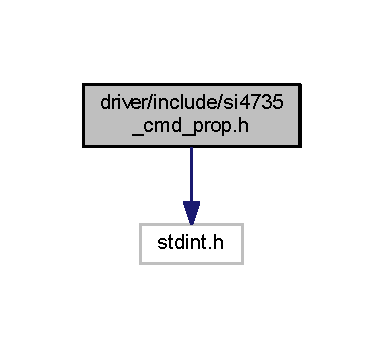
\includegraphics[width=184pt]{si4735__cmd__prop_8h__incl}
\end{center}
\end{figure}
Dieser Graph zeigt, welche Datei direkt oder indirekt diese Datei enthält\+:\nopagebreak
\begin{figure}[H]
\begin{center}
\leavevmode
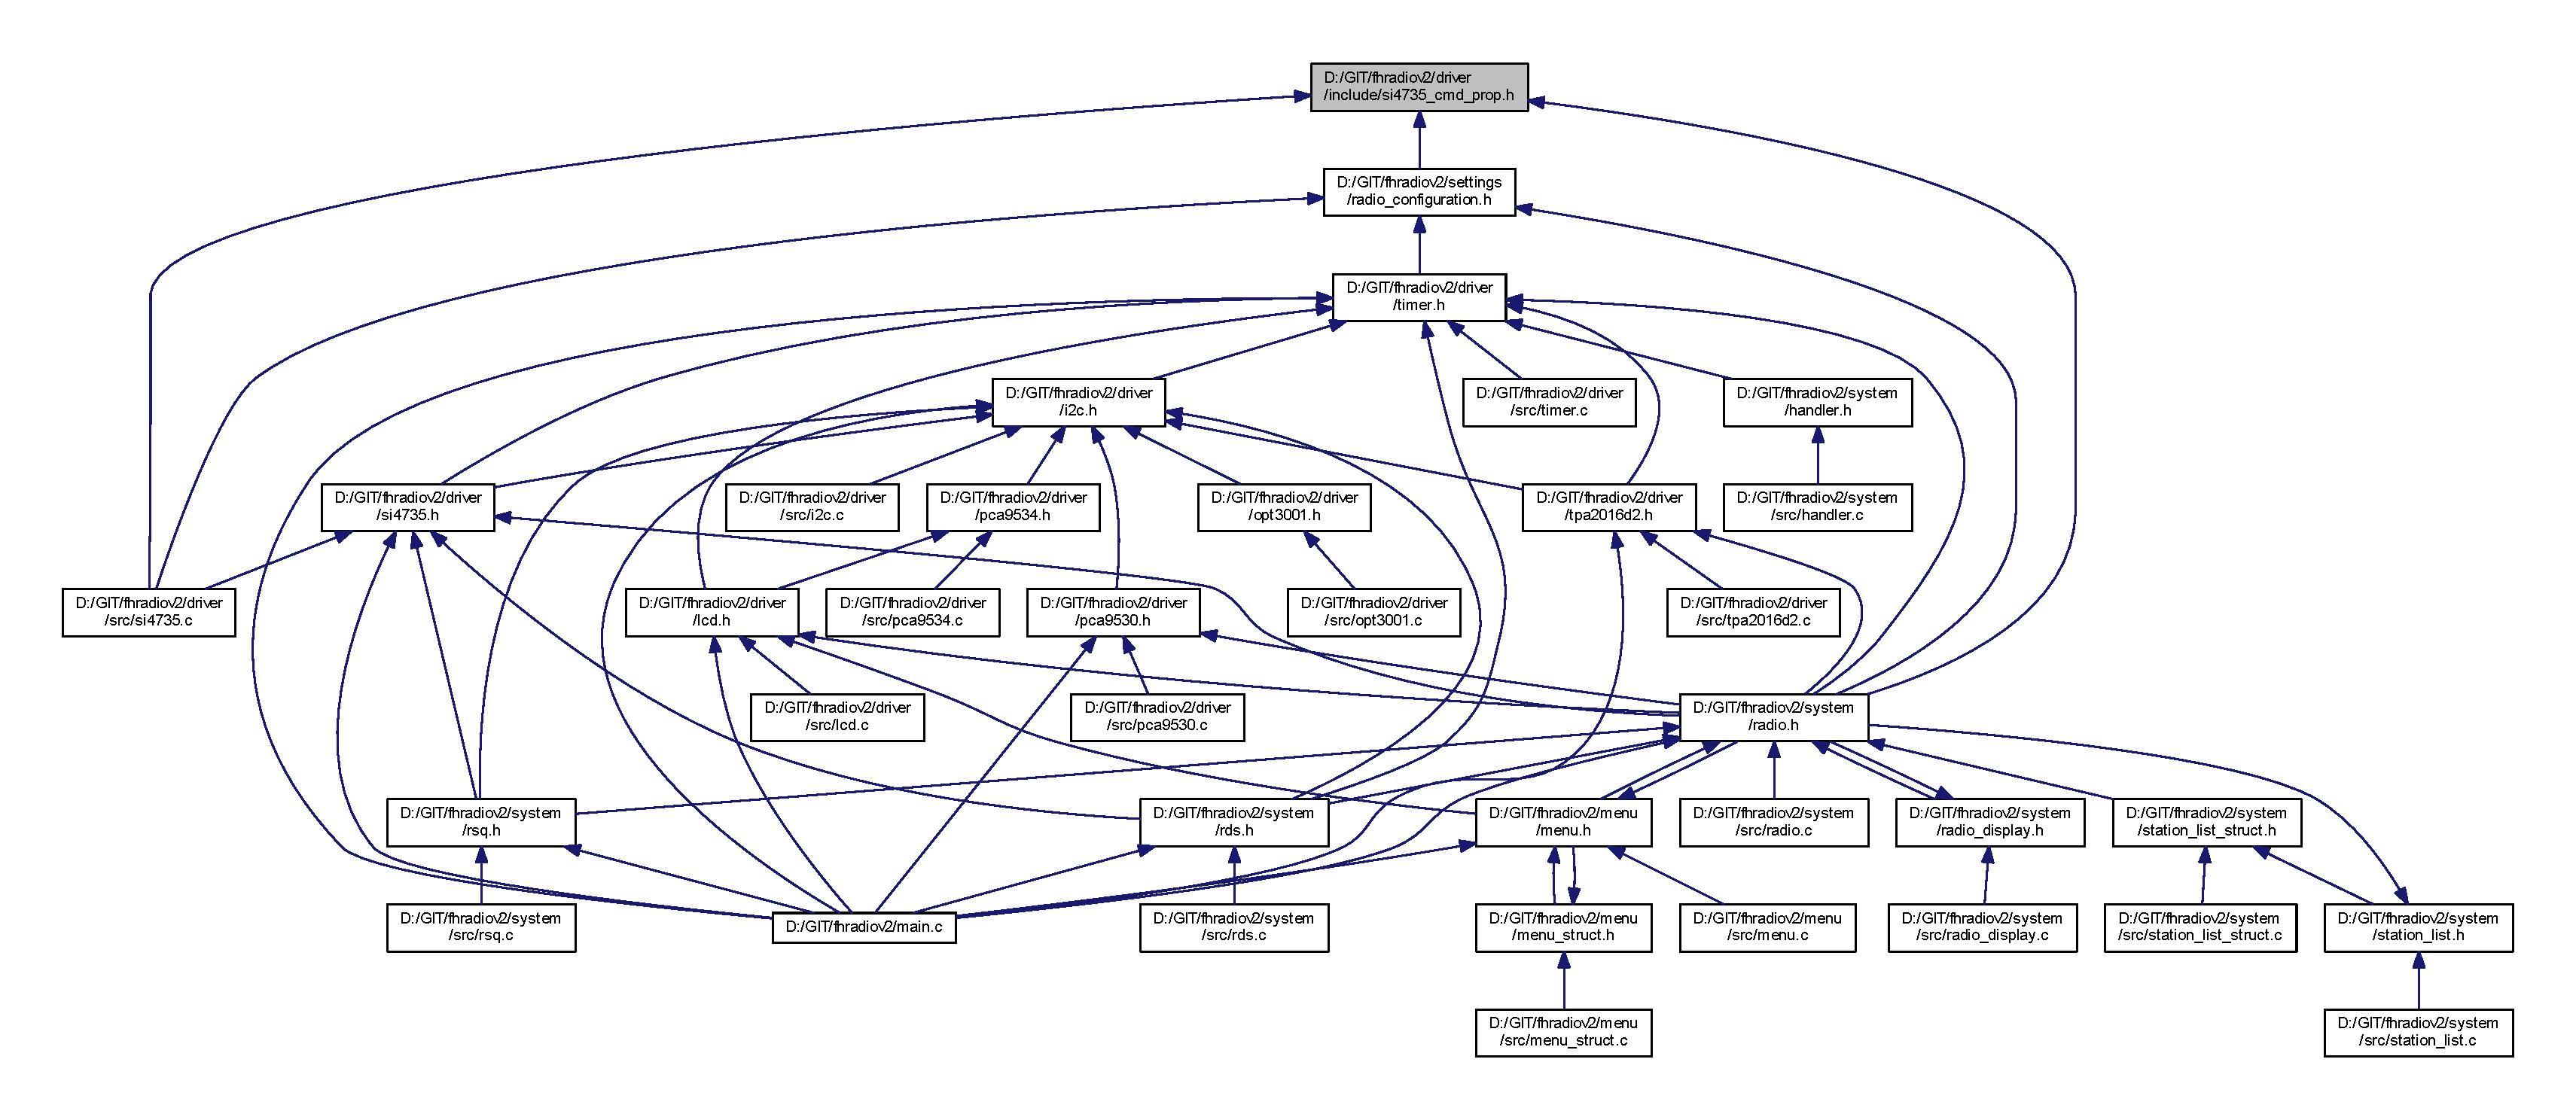
\includegraphics[width=350pt]{si4735__cmd__prop_8h__dep__incl}
\end{center}
\end{figure}
\subsection*{Datenstrukturen}
\begin{DoxyCompactItemize}
\item 
union \hyperlink{unionint__status}{int\+\_\+status}
\item 
union \hyperlink{unionpower__up__arg1}{power\+\_\+up\+\_\+arg1}
\item 
union \hyperlink{unionfm__tune__freq__arg1}{fm\+\_\+tune\+\_\+freq\+\_\+arg1}
\item 
union \hyperlink{unionfm__seek__start__arg1}{fm\+\_\+seek\+\_\+start\+\_\+arg1}
\item 
union \hyperlink{unionfm__tune__status__arg1}{fm\+\_\+tune\+\_\+status\+\_\+arg1}
\item 
union \hyperlink{unionfm__tune__status__resp1}{fm\+\_\+tune\+\_\+status\+\_\+resp1}
\item 
union \hyperlink{unionfm__rsq__status__arg1}{fm\+\_\+rsq\+\_\+status\+\_\+arg1}
\item 
union \hyperlink{unionfm__rsq__status__resp1}{fm\+\_\+rsq\+\_\+status\+\_\+resp1}
\item 
union \hyperlink{unionfm__rsq__status__resp2}{fm\+\_\+rsq\+\_\+status\+\_\+resp2}
\item 
union \hyperlink{unionfm__rsq__status__resp3}{fm\+\_\+rsq\+\_\+status\+\_\+resp3}
\item 
union \hyperlink{unionfm__rds__status__arg1}{fm\+\_\+rds\+\_\+status\+\_\+arg1}
\item 
union \hyperlink{unionfm__rds__status__resp1}{fm\+\_\+rds\+\_\+status\+\_\+resp1}
\item 
union \hyperlink{unionfm__rds__status__resp2}{fm\+\_\+rds\+\_\+status\+\_\+resp2}
\item 
union \hyperlink{unionfm__rds__status__resp12}{fm\+\_\+rds\+\_\+status\+\_\+resp12}
\item 
union \hyperlink{unionfm__agc__status__resp1}{fm\+\_\+agc\+\_\+status\+\_\+resp1}
\item 
union \hyperlink{unionfm__agc__status__resp2}{fm\+\_\+agc\+\_\+status\+\_\+resp2}
\item 
union \hyperlink{unionfm__agc__override__arg1}{fm\+\_\+agc\+\_\+override\+\_\+arg1}
\item 
union \hyperlink{unionfm__agc__override__arg2}{fm\+\_\+agc\+\_\+override\+\_\+arg2}
\item 
union \hyperlink{unionfm__gpio__ctl__arg1}{fm\+\_\+gpio\+\_\+ctl\+\_\+arg1}
\item 
union \hyperlink{unionfm__gpio__set__arg1}{fm\+\_\+gpio\+\_\+set\+\_\+arg1}
\item 
struct \hyperlink{uniongpo__ien}{gpo\+\_\+ien}
\begin{DoxyCompactList}\small\item\em Property 0x0001. G\+P\+O\+\_\+\+I\+E\+N. \end{DoxyCompactList}\item 
struct \hyperlink{uniondout__format}{dout\+\_\+format}
\begin{DoxyCompactList}\small\item\em Property 0x0102. D\+I\+G\+I\+T\+A\+L\+\_\+\+O\+U\+T\+P\+U\+T\+\_\+\+F\+O\+R\+M\+A\+T. \end{DoxyCompactList}\item 
union \hyperlink{unionrefclk__pre}{refclk\+\_\+pre}
\item 
union \hyperlink{unionfm__deemphasis}{fm\+\_\+deemphasis}
\item 
union \hyperlink{unionfm__channel__filter}{fm\+\_\+channel\+\_\+filter}
\item 
union \hyperlink{unionfm__blend__stereo}{fm\+\_\+blend\+\_\+stereo}
\item 
union \hyperlink{unionfm__blend__mono}{fm\+\_\+blend\+\_\+mono}
\item 
union \hyperlink{unionfm__max__tune__err}{fm\+\_\+max\+\_\+tune\+\_\+err}
\item 
union \hyperlink{unionfm__rsq__int__source}{fm\+\_\+rsq\+\_\+int\+\_\+source}
\item 
union \hyperlink{unionfm__rsq__snr__hi__thres}{fm\+\_\+rsq\+\_\+snr\+\_\+hi\+\_\+thres}
\item 
union \hyperlink{unionfm__rsq__snr__lo__thres}{fm\+\_\+rsq\+\_\+snr\+\_\+lo\+\_\+thres}
\item 
union \hyperlink{unionfm__rsq__rssi__hi__thres}{fm\+\_\+rsq\+\_\+rssi\+\_\+hi\+\_\+thres}
\item 
union \hyperlink{unionfm__rsq__rssi__lo__thres}{fm\+\_\+rsq\+\_\+rssi\+\_\+lo\+\_\+thres}
\item 
union \hyperlink{unionfm__rsq__multi__hi__thres}{fm\+\_\+rsq\+\_\+multi\+\_\+hi\+\_\+thres}
\item 
union \hyperlink{unionfm__rsq__multi__lo__thres}{fm\+\_\+rsq\+\_\+multi\+\_\+lo\+\_\+thres}
\item 
union \hyperlink{unionfm__rsq__blend__thres}{fm\+\_\+rsq\+\_\+blend\+\_\+thres}
\item 
union \hyperlink{unionfm__soft__mute__rate}{fm\+\_\+soft\+\_\+mute\+\_\+rate}
\item 
union \hyperlink{unionfm__soft__mute__slope}{fm\+\_\+soft\+\_\+mute\+\_\+slope}
\item 
union \hyperlink{unionfm__soft__mute__max__att}{fm\+\_\+soft\+\_\+mute\+\_\+max\+\_\+att}
\item 
union \hyperlink{unionfm__soft__mute__snr__thres}{fm\+\_\+soft\+\_\+mute\+\_\+snr\+\_\+thres}
\item 
union \hyperlink{unionfm__soft__mute__rel__rate}{fm\+\_\+soft\+\_\+mute\+\_\+rel\+\_\+rate}
\item 
union \hyperlink{unionfm__soft__mute__atk__rate}{fm\+\_\+soft\+\_\+mute\+\_\+atk\+\_\+rate}
\item 
union \hyperlink{unionfm__seek__freq__spacing}{fm\+\_\+seek\+\_\+freq\+\_\+spacing}
\item 
union \hyperlink{unionfm__seek__tune__snr__thres}{fm\+\_\+seek\+\_\+tune\+\_\+snr\+\_\+thres}
\item 
union \hyperlink{unionfm__seek__tune__rssi__thres}{fm\+\_\+seek\+\_\+tune\+\_\+rssi\+\_\+thres}
\item 
union \hyperlink{unionfm__rds__int__source}{fm\+\_\+rds\+\_\+int\+\_\+source}
\item 
union \hyperlink{unionfm__rds__int__fifo__count}{fm\+\_\+rds\+\_\+int\+\_\+fifo\+\_\+count}
\item 
union \hyperlink{unionfm__rds__config}{fm\+\_\+rds\+\_\+config}
\item 
union \hyperlink{unionfm__rds__confidence}{fm\+\_\+rds\+\_\+confidence}
\item 
union \hyperlink{unionfm__agc__atk__rate}{fm\+\_\+agc\+\_\+atk\+\_\+rate}
\item 
union \hyperlink{unionfm__agc__rel__rate}{fm\+\_\+agc\+\_\+rel\+\_\+rate}
\item 
union \hyperlink{unionfm__blend__rssi__stero__thres}{fm\+\_\+blend\+\_\+rssi\+\_\+stero\+\_\+thres}
\item 
union \hyperlink{unionfm__blend__rssi__mono__thres}{fm\+\_\+blend\+\_\+rssi\+\_\+mono\+\_\+thres}
\item 
union \hyperlink{unionfm__blend__snr__stereo__thres}{fm\+\_\+blend\+\_\+snr\+\_\+stereo\+\_\+thres}
\item 
union \hyperlink{unionfm__blend__snr__mono__thres}{fm\+\_\+blend\+\_\+snr\+\_\+mono\+\_\+thres}
\item 
union \hyperlink{unionfm__blend__multi__stereo__thres}{fm\+\_\+blend\+\_\+multi\+\_\+stereo\+\_\+thres}
\item 
union \hyperlink{unionfm__blend__multi__mono__thres}{fm\+\_\+blend\+\_\+multi\+\_\+mono\+\_\+thres}
\item 
union \hyperlink{unionfm__blend__max__stereo__sepa}{fm\+\_\+blend\+\_\+max\+\_\+stereo\+\_\+sepa}
\item 
union \hyperlink{unionfm__hicut__snr__high__thres}{fm\+\_\+hicut\+\_\+snr\+\_\+high\+\_\+thres}
\item 
union \hyperlink{unionfm__hicut__snr__low__thres}{fm\+\_\+hicut\+\_\+snr\+\_\+low\+\_\+thres}
\item 
union \hyperlink{unionfm__hicut__multi__trigger__thres}{fm\+\_\+hicut\+\_\+multi\+\_\+trigger\+\_\+thres}
\item 
union \hyperlink{unionfm__hicut__multi__end__thres}{fm\+\_\+hicut\+\_\+multi\+\_\+end\+\_\+thres}
\item 
union \hyperlink{unionfm__hicut__cutoff__freq}{fm\+\_\+hicut\+\_\+cutoff\+\_\+freq}
\item 
union \hyperlink{unionrx__volume}{rx\+\_\+volume}
\item 
union \hyperlink{unionrx__hard__mute}{rx\+\_\+hard\+\_\+mute}
\end{DoxyCompactItemize}
\subsection*{Makrodefinitionen}
\begin{DoxyCompactItemize}
\item 
\#define \hyperlink{si4735__cmd__prop_8h_a4c189ed5b7ef570b7e084edd7389c410}{H\+B}(byte)~((byte \& 0x\+F\+F00) $>$$>$ 8)
\item 
\#define \hyperlink{si4735__cmd__prop_8h_ac8008518fa109d79d7c6676c517b9597}{L\+B}(byte)~(byte \& 0x00\+F\+F)
\item 
\#define \hyperlink{si4735__cmd__prop_8h_abf6b929a6f72c48fdb78218394541db2}{P\+O\+W\+E\+R\+\_\+\+U\+P}~0x01
\item 
\#define \hyperlink{si4735__cmd__prop_8h_a3f73fba7deaa34ba40b8ceec0944c471}{F\+U\+N\+C\+\_\+0}~0x00
\item 
\#define \hyperlink{si4735__cmd__prop_8h_aaac3c29e7e33c0ed3a79638fb45e5134}{F\+U\+N\+C\+\_\+1}~0x0\+F
\item 
\#define \hyperlink{si4735__cmd__prop_8h_a30a2dd557634ac82608ed79cdfe07a9a}{O\+P\+M\+O\+D\+E\+\_\+0}~0x00
\item 
\#define \hyperlink{si4735__cmd__prop_8h_a20fc7e4857cf8d5c09902ee284c574bb}{O\+P\+M\+O\+D\+E\+\_\+1}~0x05
\item 
\#define \hyperlink{si4735__cmd__prop_8h_a80a2dc4a82678aad621aa80eb4f0ad52}{O\+P\+M\+O\+D\+E\+\_\+2}~0x0\+B
\item 
\#define \hyperlink{si4735__cmd__prop_8h_a7fcbc66bfbdbda3e1b65ed31526af0a9}{O\+P\+M\+O\+D\+E\+\_\+3}~0x\+B0
\item 
\#define \hyperlink{si4735__cmd__prop_8h_afbac76ee7ce6218df991f20276f28617}{O\+P\+M\+O\+D\+E\+\_\+4}~0x\+B5
\item 
\#define \hyperlink{si4735__cmd__prop_8h_a9fbb31eec68a8b17895fd18640296013}{G\+E\+T\+\_\+\+R\+E\+V}~0x10
\item 
\#define \hyperlink{si4735__cmd__prop_8h_aad04e0c9afdeec307d5b9cb2062d784d}{P\+O\+W\+E\+R\+\_\+\+D\+O\+W\+N}~0x11
\item 
\#define \hyperlink{si4735__cmd__prop_8h_a92cfecd26935c8864d65bbdc6031acb0}{S\+E\+T\+\_\+\+P\+R\+O\+P\+E\+R\+T\+Y}~0x12
\item 
\#define \hyperlink{si4735__cmd__prop_8h_acf7a3971c551fcdf7ae16bb0f31c149d}{G\+E\+T\+\_\+\+P\+R\+O\+P\+E\+R\+T\+Y}~0x13
\item 
\#define \hyperlink{si4735__cmd__prop_8h_ab34642df1357e9ee8ecd90913bdae01f}{G\+E\+T\+\_\+\+I\+N\+T\+\_\+\+S\+T\+A\+T\+U\+S}~0x14
\item 
\#define \hyperlink{si4735__cmd__prop_8h_aa9acf37dc2ae6e26a01780d6d4e6dcc1}{F\+M\+\_\+\+T\+U\+N\+E\+\_\+\+F\+R\+E\+Q}~0x20
\item 
\#define \hyperlink{si4735__cmd__prop_8h_a25ef5653fc9206ab83d8215c209e9922}{F\+M\+\_\+\+S\+E\+E\+K\+\_\+\+S\+T\+A\+R\+T}~0x21
\item 
\#define \hyperlink{si4735__cmd__prop_8h_a1c2be0c09ef2120b4e7b6d050a4a7735}{F\+M\+\_\+\+T\+U\+N\+E\+\_\+\+S\+T\+A\+T\+U\+S}~0x22
\item 
\#define \hyperlink{si4735__cmd__prop_8h_a9b58aeaeabdad7b1525ccc31f5d0d201}{F\+M\+\_\+\+R\+S\+Q\+\_\+\+S\+T\+A\+T\+U\+S}~0x23
\item 
\#define \hyperlink{si4735__cmd__prop_8h_ac37ef03bb47367289779f5f9bc00b18f}{F\+M\+\_\+\+R\+D\+S\+\_\+\+S\+T\+A\+T\+U\+S}~0x24
\item 
\#define \hyperlink{si4735__cmd__prop_8h_ac5bbf51a4a4b25c538375567c2f4c8dc}{F\+M\+\_\+\+A\+G\+C\+\_\+\+S\+T\+A\+T\+U\+S}~0x27
\item 
\#define \hyperlink{si4735__cmd__prop_8h_a805bf3e7373f81190388810992fa17ae}{F\+M\+\_\+\+A\+G\+C\+\_\+\+O\+V\+E\+R\+R\+I\+D\+E}~0x28
\item 
\#define \hyperlink{si4735__cmd__prop_8h_ac4ede73dbac84ceab4a5bc876104bc20}{G\+P\+I\+O\+\_\+\+C\+T\+L}~0x80
\item 
\#define \hyperlink{si4735__cmd__prop_8h_aee1a56baeb6b8457fb722fd36dad5bbf}{G\+P\+I\+O\+\_\+\+S\+E\+T}~0x81
\item 
\#define \hyperlink{si4735__cmd__prop_8h_a16b9c6d556c2db79e8742267daf63c83}{G\+P\+O\+\_\+\+I\+E\+N}~0x0001
\begin{DoxyCompactList}\small\item\em Property for the F\+M/\+R\+D\+S Receiver (Si4704/05/06/2x/3x/4x/84/85), required struct \hyperlink{uniongpo__ien}{gpo\+\_\+ien}. \end{DoxyCompactList}\item 
\#define \hyperlink{si4735__cmd__prop_8h_ade54244495ac2a6ddd8102851112fb82}{D\+O\+U\+T\+\_\+\+F\+O\+R\+M\+A\+T}~0x0102
\begin{DoxyCompactList}\small\item\em Property for the F\+M/\+R\+D\+S Receiver (Si4704/05/06/2x/3x/4x/84/85), required struct \hyperlink{uniondout__format}{dout\+\_\+format}. \end{DoxyCompactList}\item 
\#define \hyperlink{si4735__cmd__prop_8h_a97eb55330da3ef82f52a1812b06a3c36}{O\+M\+O\+D\+E\+\_\+0}~0
\begin{DoxyCompactList}\small\item\em Digital Output Mode 0000 = I2\+Suse for \hyperlink{uniondout__format_a4d995054bef39e68df20343ec82ae5b9}{dout\+\_\+format\+::\+O\+M\+O\+D\+E}. \end{DoxyCompactList}\item 
\#define \hyperlink{si4735__cmd__prop_8h_a24cba45377ab16544630a55632078d09}{O\+M\+O\+D\+E\+\_\+1}~6
\begin{DoxyCompactList}\small\item\em Digital Output Mode 0110 = Left-\/justifieduse for \hyperlink{uniondout__format_a4d995054bef39e68df20343ec82ae5b9}{dout\+\_\+format\+::\+O\+M\+O\+D\+E}. \end{DoxyCompactList}\item 
\#define \hyperlink{si4735__cmd__prop_8h_ade93d9729553e27d9cd14a267587339e}{O\+M\+O\+D\+E\+\_\+2}~8
\begin{DoxyCompactList}\small\item\em Digital Output Mode 1000 = M\+S\+B at second D\+C\+L\+K after D\+F\+S pulse, use for \hyperlink{uniondout__format_a4d995054bef39e68df20343ec82ae5b9}{dout\+\_\+format\+::\+O\+M\+O\+D\+E}. \end{DoxyCompactList}\item 
\#define \hyperlink{si4735__cmd__prop_8h_a3cfe4a4e0a57d9e803a167e692b2c6d8}{O\+M\+O\+D\+E\+\_\+3}~12
\begin{DoxyCompactList}\small\item\em Digital Output Mode 1100 = M\+S\+B at first D\+C\+L\+K after D\+F\+S pulse, use for \hyperlink{uniondout__format_a4d995054bef39e68df20343ec82ae5b9}{dout\+\_\+format\+::\+O\+M\+O\+D\+E}. \end{DoxyCompactList}\item 
\#define \hyperlink{si4735__cmd__prop_8h_a160b540283defaa95e4d08adc814dee6}{O\+S\+I\+Z\+E\+\_\+0}~0
\begin{DoxyCompactList}\small\item\em Digital Output Audio Sample Precision 0 = 16 bits, use for \hyperlink{uniondout__format_a7b03eaf984aaf8efadcedcfabd0df922}{dout\+\_\+format\+::\+O\+S\+I\+Z\+E}. \end{DoxyCompactList}\item 
\#define \hyperlink{si4735__cmd__prop_8h_a193efff6f159e280fca20f0622b854d2}{O\+S\+I\+Z\+E\+\_\+1}~1
\begin{DoxyCompactList}\small\item\em Digital Output Audio Sample Precision 1 = 20 bits, use for \hyperlink{uniondout__format_a7b03eaf984aaf8efadcedcfabd0df922}{dout\+\_\+format\+::\+O\+S\+I\+Z\+E}. \end{DoxyCompactList}\item 
\#define \hyperlink{si4735__cmd__prop_8h_ae7fe445f1a936b0daf0b328daba6b94f}{O\+S\+I\+Z\+E\+\_\+2}~2
\begin{DoxyCompactList}\small\item\em Digital Output Audio Sample Precision 2 = 24 bits, use for \hyperlink{uniondout__format_a7b03eaf984aaf8efadcedcfabd0df922}{dout\+\_\+format\+::\+O\+S\+I\+Z\+E}. \end{DoxyCompactList}\item 
\#define \hyperlink{si4735__cmd__prop_8h_ab59b8a87da28ccd035507e878e6b8474}{O\+S\+I\+Z\+E\+\_\+3}~3
\begin{DoxyCompactList}\small\item\em Digital Output Audio Sample Precision 3 = 8 bits, use for \hyperlink{uniondout__format_a7b03eaf984aaf8efadcedcfabd0df922}{dout\+\_\+format\+::\+O\+S\+I\+Z\+E}. \end{DoxyCompactList}\item 
\#define \hyperlink{si4735__cmd__prop_8h_a0ac469bcc5b7cfeb3e81528a792542c7}{D\+O\+U\+T\+\_\+\+S\+A\+M\+P\+L\+E\+\_\+\+R\+A\+T\+E}~0x0104
\item 
\#define \hyperlink{si4735__cmd__prop_8h_adb330b20b383f5f664a9b107edef0036}{R\+E\+F\+C\+L\+K\+\_\+\+F\+R\+E\+Q}~0x0201
\item 
\#define \hyperlink{si4735__cmd__prop_8h_a6b615b86f7870b616243b25cb5091933}{R\+E\+F\+C\+L\+K\+\_\+\+P\+R\+E\+S\+C\+A\+L\+E}~0x0202
\item 
\#define \hyperlink{si4735__cmd__prop_8h_a1c7743943a1def297fe209d001d49c1e}{F\+M\+\_\+\+D\+E\+E\+M\+P\+H}~0x1100
\item 
\#define \hyperlink{si4735__cmd__prop_8h_a3390ee4d2cdcaf28cc7df2390d70e10a}{D\+E\+E\+M\+P\+H\+\_\+\+U\+S}~2
\item 
\#define \hyperlink{si4735__cmd__prop_8h_afa8b508d6e40dc9c4f4430d46290a919}{D\+E\+E\+M\+P\+H\+\_\+\+E\+U}~1
\item 
\#define \hyperlink{si4735__cmd__prop_8h_a256c5d4d465c20695770fdd1da7f1be5}{F\+M\+\_\+\+C\+H\+\_\+\+F\+I\+L}~0x1102
\item 
\#define \hyperlink{si4735__cmd__prop_8h_ab068e5e6453d39752e0203b3a3b4a251}{F\+M\+\_\+\+F\+I\+L\+T\+E\+R\+\_\+\+A\+U\+T\+O}~0
\item 
\#define \hyperlink{si4735__cmd__prop_8h_a0173ae46aaee5563698b23f56b2a8317}{F\+M\+\_\+\+F\+I\+L\+T\+E\+R\+\_\+110\+K\+H\+Z}~1
\item 
\#define \hyperlink{si4735__cmd__prop_8h_af0242d8fab4f95f18051c4b849ae9fd4}{F\+M\+\_\+\+F\+I\+L\+T\+E\+R\+\_\+84\+K\+H\+Z}~2
\item 
\#define \hyperlink{si4735__cmd__prop_8h_a284cbb5a9340a060b8fd5854a7ca9dc8}{F\+M\+\_\+\+F\+I\+L\+T\+E\+R\+\_\+60\+K\+H\+Z}~3
\item 
\#define \hyperlink{si4735__cmd__prop_8h_a6526c86451f453640220b04687a659d4}{F\+M\+\_\+\+F\+I\+L\+T\+E\+R\+\_\+40\+K\+H\+Z}~4
\item 
\#define \hyperlink{si4735__cmd__prop_8h_a72190cac11d785ca73f0259443f45b56}{F\+M\+\_\+\+B\+L\+E\+N\+D\+\_\+\+S\+T\+E\+R\+E\+O}~0x1105
\item 
\#define \hyperlink{si4735__cmd__prop_8h_a520e490aa1daa5670e54b3812f5181ba}{F\+M\+\_\+\+B\+L\+E\+N\+D\+\_\+\+M\+O\+N\+O}~0x1106
\item 
\#define \hyperlink{si4735__cmd__prop_8h_af337ab3d5f7898bc4ddbcb05dafddcf3}{F\+M\+\_\+\+M\+A\+X\+\_\+\+T\+U\+N\+E\+\_\+\+E\+R\+R}~0x1108
\item 
\#define \hyperlink{si4735__cmd__prop_8h_a018d7b17a85e732ee11cf91f5be5935c}{F\+M\+\_\+\+R\+S\+Q\+\_\+\+I\+N\+T\+\_\+\+S\+O\+U\+R\+C\+E}~0x1200
\item 
\#define \hyperlink{si4735__cmd__prop_8h_a51745c323327afd9637aecb45bb04cf9}{F\+M\+\_\+\+R\+S\+Q\+\_\+\+S\+N\+R\+\_\+\+H\+I\+\_\+\+T\+H\+R\+E\+S}~0x1201
\item 
\#define \hyperlink{si4735__cmd__prop_8h_a1134735e2f2376e54d6d282ba1428bd6}{F\+M\+\_\+\+R\+S\+Q\+\_\+\+S\+N\+R\+\_\+\+L\+O\+\_\+\+T\+H\+R\+E\+S}~0x1202
\item 
\#define \hyperlink{si4735__cmd__prop_8h_ad00533ed6bc3aa10dc9be7c18edba58e}{F\+M\+\_\+\+R\+S\+Q\+\_\+\+R\+S\+S\+I\+\_\+\+H\+I\+\_\+\+T\+H\+R\+E\+S}~0x1203
\item 
\#define \hyperlink{si4735__cmd__prop_8h_a45ef59340f8fcbc9ec9599f0a5321b18}{F\+M\+\_\+\+R\+S\+Q\+\_\+\+R\+S\+S\+I\+\_\+\+L\+O\+\_\+\+T\+H\+R\+E\+S}~0x1204
\item 
\#define \hyperlink{si4735__cmd__prop_8h_accff344d93fb5cf52e71e751cbaacdc9}{F\+M\+\_\+\+R\+S\+Q\+\_\+\+M\+U\+L\+T\+I\+\_\+\+H\+I\+\_\+\+T\+H\+R\+E\+S}~0x1205
\item 
\#define \hyperlink{si4735__cmd__prop_8h_adaa4011283ef80cf38855396fb66fdf0}{F\+M\+\_\+\+R\+S\+Q\+\_\+\+M\+U\+L\+T\+I\+\_\+\+L\+O\+\_\+\+T\+H\+R\+E\+S}~0x1206
\item 
\#define \hyperlink{si4735__cmd__prop_8h_a00f00e3d67d6c0411efb14ead6313163}{F\+M\+\_\+\+R\+S\+Q\+\_\+\+B\+L\+E\+N\+D\+\_\+\+T\+H\+R\+E\+S}~0x1207
\item 
\#define \hyperlink{si4735__cmd__prop_8h_a071a5bbf23d933861cb73987c74e9fed}{F\+M\+\_\+\+S\+O\+F\+T\+\_\+\+M\+U\+T\+E\+\_\+\+R\+A\+T\+E}~0x1300
\item 
\#define \hyperlink{si4735__cmd__prop_8h_ad90847770bc9057d28c2db4975a37ab5}{F\+M\+\_\+\+S\+O\+F\+T\+\_\+\+M\+U\+T\+E\+\_\+\+S\+L\+O\+P\+E}~0x1301
\item 
\#define \hyperlink{si4735__cmd__prop_8h_ae347e93e87d54e491a31d6c3a0bd4373}{F\+M\+\_\+\+S\+O\+F\+T\+\_\+\+M\+U\+T\+E\+\_\+\+M\+A\+X\+\_\+\+A\+T\+T}~0x1302
\item 
\#define \hyperlink{si4735__cmd__prop_8h_aa23b099f4ffaf736b3f2f083e228837b}{F\+M\+\_\+\+S\+O\+F\+T\+\_\+\+M\+U\+T\+E\+\_\+\+S\+N\+R\+\_\+\+T\+H\+R\+E\+S}~0x1303
\item 
\#define \hyperlink{si4735__cmd__prop_8h_a19209ef7d0fc954473d842ded516b948}{F\+M\+\_\+\+S\+O\+F\+T\+\_\+\+M\+U\+T\+E\+\_\+\+R\+E\+L\+\_\+\+R\+A\+T\+E}~0x1301
\item 
\#define \hyperlink{si4735__cmd__prop_8h_a98eeba9b8426811fbab59e7a0d56684d}{F\+M\+\_\+\+S\+O\+F\+T\+\_\+\+M\+U\+T\+E\+\_\+\+A\+T\+K\+\_\+\+R\+A\+T\+E}~0x1305
\item 
\#define \hyperlink{si4735__cmd__prop_8h_a17c1d20d698569b77c2d00fb03fc905a}{F\+M\+\_\+\+S\+E\+E\+K\+\_\+\+B\+A\+N\+D\+\_\+\+B\+O\+T\+T\+O\+M}~0x1400
\item 
\#define \hyperlink{si4735__cmd__prop_8h_ae8f8164aecb98eb67811957866f7173a}{F\+M\+\_\+\+S\+E\+E\+K\+\_\+\+B\+A\+N\+D\+\_\+\+T\+O\+P}~0x1401
\item 
\#define \hyperlink{si4735__cmd__prop_8h_ac5a0322f265c6a26f2eaa67b137a4e1e}{F\+M\+\_\+\+S\+E\+E\+K\+\_\+\+F\+R\+E\+Q\+\_\+\+S\+P\+A\+C\+I\+N\+G}~0x1402
\item 
\#define \hyperlink{si4735__cmd__prop_8h_ab96cd70051b2a1b7ef1d331e757e3320}{S\+K\+S\+P\+A\+C\+E\+\_\+5}~0x0005
\item 
\#define \hyperlink{si4735__cmd__prop_8h_a22aafccbeb6b71e338f6ab4198576477}{S\+K\+S\+P\+A\+C\+E\+\_\+10}~0x000\+A
\item 
\#define \hyperlink{si4735__cmd__prop_8h_a8bfa5a728fd5226e3900c133c001cead}{S\+K\+S\+P\+A\+C\+E\+\_\+20}~0x0014
\item 
\#define \hyperlink{si4735__cmd__prop_8h_a8159dc3f7948223302c72404f8b3b7df}{F\+M\+\_\+\+S\+E\+E\+K\+\_\+\+T\+U\+N\+E\+\_\+\+S\+N\+R\+\_\+\+T\+H\+R\+E\+S}~0x1403
\item 
\#define \hyperlink{si4735__cmd__prop_8h_a855621fba4889ce1231a6eec81080d37}{F\+M\+\_\+\+S\+E\+E\+K\+\_\+\+T\+U\+N\+E\+\_\+\+R\+S\+S\+I\+\_\+\+T\+H\+R\+E\+S}~0x1404
\item 
\#define \hyperlink{si4735__cmd__prop_8h_a8b7e6ccffb54cef940f3bd78d255bc36}{F\+M\+\_\+\+R\+D\+S\+\_\+\+I\+N\+T\+\_\+\+S\+O\+U\+R\+C\+E}~0x1500
\item 
\#define \hyperlink{si4735__cmd__prop_8h_afdc3800cf259f4c1acb254d1ad61f21b}{F\+M\+\_\+\+R\+D\+S\+\_\+\+I\+N\+T\+\_\+\+F\+I\+F\+O\+\_\+\+C\+O\+U\+N\+T}~0x1501
\item 
\#define \hyperlink{si4735__cmd__prop_8h_afbaa25e11748b1bd64456d3eae79fdee}{F\+M\+\_\+\+R\+D\+S\+\_\+\+C\+O\+N\+F\+I\+G}~0x1502
\item 
\#define \hyperlink{si4735__cmd__prop_8h_affc8ead3ceabdcc4088ee13e1714476f}{B\+L\+E\+T\+H\+\_\+\+N\+O\+\_\+\+E\+R\+R}~0
\item 
\#define \hyperlink{si4735__cmd__prop_8h_a423186489dc9a9dbdd8d704d7d1eb367}{B\+L\+E\+T\+H\+\_\+1\+\_\+2\+\_\+\+E\+R\+R}~1
\item 
\#define \hyperlink{si4735__cmd__prop_8h_af050b413775dcd5845108d44ee3cce5b}{B\+L\+E\+T\+H\+\_\+3\+\_\+5\+\_\+\+E\+R\+R}~2
\item 
\#define \hyperlink{si4735__cmd__prop_8h_af08cabdaf63f8a7e29cee45af5401591}{B\+L\+E\+T\+H\+\_\+\+N\+O\+\_\+\+C\+O\+R\+R}~3
\item 
\#define \hyperlink{si4735__cmd__prop_8h_a6651f2bcc216c9b0950999f70bf2be44}{F\+M\+\_\+\+R\+D\+S\+\_\+\+C\+O\+N\+F\+I\+D\+E\+N\+C\+E}~0x1503
\item 
\#define \hyperlink{si4735__cmd__prop_8h_a0291c50cbfd6f81bb405e7cfa4b9540e}{F\+M\+\_\+\+A\+G\+C\+\_\+\+A\+T\+K\+\_\+\+R\+A\+T\+E}~0x1700
\item 
\#define \hyperlink{si4735__cmd__prop_8h_abd6dfe2cc7a4ba792483c61931e86399}{F\+M\+\_\+\+A\+G\+C\+\_\+\+R\+E\+L\+\_\+\+R\+A\+T\+E}~0x1701
\item 
\#define \hyperlink{si4735__cmd__prop_8h_a606875e5ce0688b3eb13a89e89a429fe}{F\+M\+\_\+\+B\+L\+E\+N\+D\+\_\+\+R\+S\+S\+I\+\_\+\+S\+T\+E\+R\+E\+O\+\_\+\+T\+H\+R\+E\+S}~0x1800
\item 
\#define \hyperlink{si4735__cmd__prop_8h_a0f35560b1ed8beb00aa5331542d9fbfa}{F\+M\+\_\+\+B\+L\+E\+N\+D\+\_\+\+R\+S\+S\+I\+\_\+\+M\+O\+N\+O\+\_\+\+T\+H\+R\+E\+S}~0x1801
\item 
\#define \hyperlink{si4735__cmd__prop_8h_a28bd159fb046b2cf69bab12cfcb84492}{F\+M\+\_\+\+B\+L\+E\+N\+D\+\_\+\+R\+S\+S\+I\+\_\+\+A\+T\+K\+\_\+\+R\+A\+T\+E}~0x1802
\item 
\#define \hyperlink{si4735__cmd__prop_8h_adbcb468549bc5bfbdbfeb1b7d5603bb9}{F\+M\+\_\+\+B\+L\+E\+N\+D\+\_\+\+R\+S\+S\+I\+\_\+\+R\+E\+L\+\_\+\+R\+A\+T\+E}~0x1803
\item 
\#define \hyperlink{si4735__cmd__prop_8h_ac0a17f169f76690610c2ddb3ec7bddee}{F\+M\+\_\+\+B\+L\+E\+N\+D\+\_\+\+S\+N\+R\+\_\+\+S\+T\+E\+R\+E\+O\+\_\+\+T\+H\+R\+E\+S}~0x1804
\item 
\#define \hyperlink{si4735__cmd__prop_8h_a8f54d932b05a134f564c5bbaf17300a4}{F\+M\+\_\+\+B\+L\+E\+N\+D\+\_\+\+S\+N\+R\+\_\+\+M\+O\+N\+O\+\_\+\+T\+H\+R\+E\+S}~0x1805
\item 
\#define \hyperlink{si4735__cmd__prop_8h_aa8062929e40ac038fb518e81e09da02e}{F\+M\+\_\+\+B\+L\+E\+N\+D\+\_\+\+S\+N\+R\+\_\+\+A\+T\+K\+\_\+\+R\+A\+T\+E}~0x1806
\item 
\#define \hyperlink{si4735__cmd__prop_8h_a99ffdf6465399664c4ae46e210df74a8}{F\+M\+\_\+\+B\+L\+E\+N\+D\+\_\+\+S\+N\+R\+\_\+\+R\+E\+L\+\_\+\+R\+A\+T\+E}~0x1807
\item 
\#define \hyperlink{si4735__cmd__prop_8h_a07a3497e504a75014b6475fd7fe2a86b}{F\+M\+\_\+\+B\+L\+E\+N\+D\+\_\+\+M\+U\+L\+T\+I\+\_\+\+S\+T\+E\+R\+E\+O\+\_\+\+T\+H\+R\+E\+S}~0x1808
\item 
\#define \hyperlink{si4735__cmd__prop_8h_aa734947288b454ef5a260bac547854a2}{F\+M\+\_\+\+B\+L\+E\+N\+D\+\_\+\+M\+U\+L\+T\+I\+\_\+\+M\+O\+N\+O\+\_\+\+T\+H\+R\+E\+S}~0x1809
\item 
\#define \hyperlink{si4735__cmd__prop_8h_a640b1a99b1d792b394758b0f671abae8}{F\+M\+\_\+\+B\+L\+E\+N\+D\+\_\+\+M\+U\+L\+T\+I\+\_\+\+A\+T\+K\+\_\+\+R\+A\+T\+E}~0x180\+A
\item 
\#define \hyperlink{si4735__cmd__prop_8h_a78be01b4a8f4beb5471b3525fd5ce1f5}{F\+M\+\_\+\+B\+L\+E\+N\+D\+\_\+\+M\+U\+L\+T\+I\+\_\+\+R\+E\+L\+\_\+\+R\+A\+T\+E}~0x180\+B
\item 
\#define \hyperlink{si4735__cmd__prop_8h_a995049c31cd6032500da41c0f6685758}{F\+M\+\_\+\+B\+L\+E\+N\+D\+\_\+\+M\+A\+X\+\_\+\+S\+T\+E\+R\+E\+O\+\_\+\+S\+E\+P\+A}~0x180\+C
\item 
\#define \hyperlink{si4735__cmd__prop_8h_a640b1a99b1d792b394758b0f671abae8}{F\+M\+\_\+\+B\+L\+E\+N\+D\+\_\+\+M\+U\+L\+T\+I\+\_\+\+A\+T\+K\+\_\+\+R\+A\+T\+E}~0x180\+A
\item 
\#define \hyperlink{si4735__cmd__prop_8h_a640b1a99b1d792b394758b0f671abae8}{F\+M\+\_\+\+B\+L\+E\+N\+D\+\_\+\+M\+U\+L\+T\+I\+\_\+\+A\+T\+K\+\_\+\+R\+A\+T\+E}~0x180\+A
\item 
\#define \hyperlink{si4735__cmd__prop_8h_a640b1a99b1d792b394758b0f671abae8}{F\+M\+\_\+\+B\+L\+E\+N\+D\+\_\+\+M\+U\+L\+T\+I\+\_\+\+A\+T\+K\+\_\+\+R\+A\+T\+E}~0x180\+A
\item 
\#define \hyperlink{si4735__cmd__prop_8h_a640b1a99b1d792b394758b0f671abae8}{F\+M\+\_\+\+B\+L\+E\+N\+D\+\_\+\+M\+U\+L\+T\+I\+\_\+\+A\+T\+K\+\_\+\+R\+A\+T\+E}~0x180\+A
\item 
\#define \hyperlink{si4735__cmd__prop_8h_a640b1a99b1d792b394758b0f671abae8}{F\+M\+\_\+\+B\+L\+E\+N\+D\+\_\+\+M\+U\+L\+T\+I\+\_\+\+A\+T\+K\+\_\+\+R\+A\+T\+E}~0x180\+A
\item 
\#define \hyperlink{si4735__cmd__prop_8h_a76b95e43c63e6a5f17df4a31a0a4f697}{F\+M\+\_\+\+H\+I\+C\+U\+T\+\_\+\+S\+N\+R\+\_\+\+H\+I\+G\+H\+\_\+\+T\+H\+R\+E\+S}~0x180\+A
\item 
\#define \hyperlink{si4735__cmd__prop_8h_a18ffbcad1c2801a790f878f886a91330}{F\+M\+\_\+\+H\+I\+C\+U\+T\+\_\+\+S\+N\+R\+\_\+\+L\+O\+W\+\_\+\+T\+H\+R\+E\+S}~0x180\+A
\item 
\#define \hyperlink{si4735__cmd__prop_8h_a7ca43d269d5de58b931a2a2c9e46d143}{F\+M\+\_\+\+H\+I\+C\+U\+T\+\_\+\+A\+T\+K\+\_\+\+R\+A\+T\+E}~0x1\+A02
\item 
\#define \hyperlink{si4735__cmd__prop_8h_aed517a0d83209baf3c01739b13474d08}{F\+M\+\_\+\+H\+I\+C\+U\+T\+\_\+\+R\+E\+L\+\_\+\+R\+A\+T\+E}~0x1\+A03
\item 
\#define \hyperlink{si4735__cmd__prop_8h_a8d8bf455f7d181eff216d7092a1dd2b3}{F\+M\+\_\+\+H\+I\+C\+U\+T\+\_\+\+M\+U\+L\+T\+I\+\_\+\+T\+R\+I\+G\+G\+E\+R\+\_\+\+T\+H\+R\+E\+S}~0x1\+A04
\item 
\#define \hyperlink{si4735__cmd__prop_8h_af9a1e6847d363b54146fabe99b9fa7c0}{F\+M\+\_\+\+H\+I\+C\+U\+T\+\_\+\+M\+U\+L\+T\+I\+\_\+\+E\+N\+D\+\_\+\+T\+H\+R\+E\+S}~0x1\+A05
\item 
\#define \hyperlink{si4735__cmd__prop_8h_a6e90d7b9bfb150acfae2109d135ed785}{F\+M\+\_\+\+H\+I\+C\+U\+T\+\_\+\+C\+U\+T\+O\+F\+F\+\_\+\+F\+R\+E\+Q}~0x1\+A06
\item 
\#define \hyperlink{si4735__cmd__prop_8h_a359769f5661b1b238c3550be21f9c7e7}{M\+A\+X\+\_\+\+A\+U\+D\+I\+O\+\_\+\+T\+R\+A\+N\+\_\+\+F\+R\+E\+Q\+\_\+\+A\+U\+T\+O\+\_\+\+B\+W}~0
\item 
\#define \hyperlink{si4735__cmd__prop_8h_ab78d37ab68c6a1636458eed046770be7}{M\+A\+X\+\_\+\+A\+U\+D\+I\+O\+\_\+\+T\+R\+A\+N\+\_\+\+F\+R\+E\+Q\+\_\+2\+K\+H\+Z}~1
\item 
\#define \hyperlink{si4735__cmd__prop_8h_afaf81173b4a2a82ba1e6c50a1b881650}{M\+A\+X\+\_\+\+A\+U\+D\+I\+O\+\_\+\+T\+R\+A\+N\+\_\+\+F\+R\+E\+Q\+\_\+3\+K\+H\+Z}~2
\item 
\#define \hyperlink{si4735__cmd__prop_8h_ad145437c137794c70113fe8f3586c684}{M\+A\+X\+\_\+\+A\+U\+D\+I\+O\+\_\+\+T\+R\+A\+N\+\_\+\+F\+R\+E\+Q\+\_\+4\+K\+H\+Z}~3
\item 
\#define \hyperlink{si4735__cmd__prop_8h_ae63dee95cdc456c2471c2d8dc24999dc}{M\+A\+X\+\_\+\+A\+U\+D\+I\+O\+\_\+\+T\+R\+A\+N\+\_\+\+F\+R\+E\+Q\+\_\+5\+K\+H\+Z}~4
\item 
\#define \hyperlink{si4735__cmd__prop_8h_a4500d49f25eb9bbc4d16504549db2635}{M\+A\+X\+\_\+\+A\+U\+D\+I\+O\+\_\+\+T\+R\+A\+N\+\_\+\+F\+R\+E\+Q\+\_\+6\+K\+H\+Z}~5
\item 
\#define \hyperlink{si4735__cmd__prop_8h_a321adcead30d5d68d902453eba98de7a}{M\+A\+X\+\_\+\+A\+U\+D\+I\+O\+\_\+\+T\+R\+A\+N\+\_\+\+F\+R\+E\+Q\+\_\+8\+K\+H\+Z}~6
\item 
\#define \hyperlink{si4735__cmd__prop_8h_ab81fe947484b91a57a457279b54a3c01}{M\+A\+X\+\_\+\+A\+U\+D\+I\+O\+\_\+\+T\+R\+A\+N\+\_\+\+F\+R\+E\+Q\+\_\+11\+K\+H\+Z}~7
\item 
\#define \hyperlink{si4735__cmd__prop_8h_a863d01a4ce59e1f08676900ea8c05979}{H\+I\+C\+U\+T\+\_\+\+A\+U\+D\+I\+O\+\_\+\+T\+R\+A\+N\+\_\+\+F\+R\+E\+Q\+\_\+\+D\+I\+S}~0
\item 
\#define \hyperlink{si4735__cmd__prop_8h_ae2dbf3058aecea5a08f5734687bb210b}{H\+I\+C\+U\+T\+\_\+\+A\+U\+D\+I\+O\+\_\+\+T\+R\+A\+N\+\_\+\+F\+R\+E\+Q\+\_\+2\+K\+H\+Z}~1
\item 
\#define \hyperlink{si4735__cmd__prop_8h_a85e4a66186c6be52c28187058365d94e}{H\+I\+C\+U\+T\+\_\+\+A\+U\+D\+I\+O\+\_\+\+T\+R\+A\+N\+\_\+\+F\+R\+E\+Q\+\_\+3\+K\+H\+Z}~2
\item 
\#define \hyperlink{si4735__cmd__prop_8h_aa9513a3159c3ddeb62d1160eb122eda6}{H\+I\+C\+U\+T\+\_\+\+A\+U\+D\+I\+O\+\_\+\+T\+R\+A\+N\+\_\+\+F\+R\+E\+Q\+\_\+4\+K\+H\+Z}~3
\item 
\#define \hyperlink{si4735__cmd__prop_8h_a6b279d608773910ffce702b0424b4ab6}{H\+I\+C\+U\+T\+\_\+\+A\+U\+D\+I\+O\+\_\+\+T\+R\+A\+N\+\_\+\+F\+R\+E\+Q\+\_\+5\+K\+H\+Z}~4
\item 
\#define \hyperlink{si4735__cmd__prop_8h_a640c0bb22468c4c1cd340a0e0616fb2b}{H\+I\+C\+U\+T\+\_\+\+A\+U\+D\+I\+O\+\_\+\+T\+R\+A\+N\+\_\+\+F\+R\+E\+Q\+\_\+6\+K\+H\+Z}~5
\item 
\#define \hyperlink{si4735__cmd__prop_8h_a32224cc55523f7020a6e9e5313db61a6}{H\+I\+C\+U\+T\+\_\+\+A\+U\+D\+I\+O\+\_\+\+T\+R\+A\+N\+\_\+\+F\+R\+E\+Q\+\_\+8\+K\+H\+Z}~6
\item 
\#define \hyperlink{si4735__cmd__prop_8h_aaa3ff8e28f4b9769cdfcfbee227b3541}{H\+I\+C\+U\+T\+\_\+\+A\+U\+D\+I\+O\+\_\+\+T\+R\+A\+N\+\_\+\+F\+R\+E\+Q\+\_\+11\+K\+H\+Z}~7
\item 
\#define \hyperlink{si4735__cmd__prop_8h_aeb1de40ffb7cb51cf4a151f5d1b746d7}{R\+X\+\_\+\+V\+O\+L\+U\+M\+E}~0x4000
\item 
\#define \hyperlink{si4735__cmd__prop_8h_a5d8cbc8d5c6630e874f1f8b14b897be2}{R\+X\+\_\+\+H\+A\+R\+D\+\_\+\+M\+U\+T\+E}~0x4001
\end{DoxyCompactItemize}
\subsection*{Typdefinitionen}
\begin{DoxyCompactItemize}
\item 
typedef union \hyperlink{unionint__status}{int\+\_\+status} \hyperlink{si4735__cmd__prop_8h_a0a6a50499ea2948f3d3c0be0e419915f}{I\+N\+T\+\_\+\+S\+T\+A\+T\+U\+S}
\item 
typedef union \hyperlink{unionpower__up__arg1}{power\+\_\+up\+\_\+arg1} \hyperlink{si4735__cmd__prop_8h_abe7547abc40d2ebba3380e747425b8f9}{P\+O\+W\+E\+R\+\_\+\+U\+P\+\_\+\+A\+R\+G1\+\_\+\+S\+T\+C}
\item 
typedef union \hyperlink{unionfm__tune__freq__arg1}{fm\+\_\+tune\+\_\+freq\+\_\+arg1} \hyperlink{si4735__cmd__prop_8h_ae7c274ac48c909a86bac2a1e1370617d}{F\+M\+\_\+\+T\+U\+N\+E\+\_\+\+F\+R\+E\+Q\+\_\+\+A\+R\+G1\+\_\+\+S\+T\+C}
\item 
typedef union \hyperlink{unionfm__seek__start__arg1}{fm\+\_\+seek\+\_\+start\+\_\+arg1} \hyperlink{si4735__cmd__prop_8h_ae4bc54e46cdff6a5e0fcf1553f04fcec}{F\+M\+\_\+\+S\+E\+E\+K\+\_\+\+S\+T\+A\+R\+T\+\_\+\+A\+R\+G1\+\_\+\+S\+T\+C}
\item 
typedef union \hyperlink{unionfm__tune__status__arg1}{fm\+\_\+tune\+\_\+status\+\_\+arg1} \hyperlink{si4735__cmd__prop_8h_a3b9f90579c6ce6b5245374c6688509f0}{F\+M\+\_\+\+T\+U\+N\+E\+\_\+\+S\+T\+A\+T\+U\+S\+\_\+\+A\+R\+G1\+\_\+\+S\+T\+C}
\item 
typedef union \hyperlink{unionfm__tune__status__resp1}{fm\+\_\+tune\+\_\+status\+\_\+resp1} \hyperlink{si4735__cmd__prop_8h_a3400257686140a8f80125c71871b26aa}{F\+M\+\_\+\+T\+U\+N\+E\+\_\+\+S\+T\+A\+T\+U\+S\+\_\+\+R\+E\+S\+P1\+\_\+\+S\+T\+C}
\item 
typedef union \hyperlink{unionfm__rsq__status__arg1}{fm\+\_\+rsq\+\_\+status\+\_\+arg1} \hyperlink{si4735__cmd__prop_8h_ae3875435c94a23d60279cfa0a8d13869}{F\+M\+\_\+\+R\+S\+Q\+\_\+\+S\+T\+A\+T\+U\+S\+\_\+\+A\+R\+G1\+\_\+\+S\+T\+C}
\item 
typedef union \hyperlink{unionfm__rsq__status__resp1}{fm\+\_\+rsq\+\_\+status\+\_\+resp1} \hyperlink{si4735__cmd__prop_8h_a869077846a233318e8225884b57fd13e}{F\+M\+\_\+\+R\+S\+Q\+\_\+\+S\+T\+A\+T\+U\+S\+\_\+\+R\+E\+S\+P1\+\_\+\+S\+T\+C}
\item 
typedef union \hyperlink{unionfm__rsq__status__resp2}{fm\+\_\+rsq\+\_\+status\+\_\+resp2} \hyperlink{si4735__cmd__prop_8h_ac654eef04d4d62119647cb47693318e9}{F\+M\+\_\+\+R\+S\+Q\+\_\+\+S\+T\+A\+T\+U\+S\+\_\+\+R\+E\+S\+P2\+\_\+\+S\+T\+C}
\item 
typedef union \hyperlink{unionfm__rsq__status__resp3}{fm\+\_\+rsq\+\_\+status\+\_\+resp3} \hyperlink{si4735__cmd__prop_8h_a079247b66bc9b1a882e33217b6046b72}{F\+M\+\_\+\+R\+S\+Q\+\_\+\+S\+T\+A\+T\+U\+S\+\_\+\+R\+E\+S\+P3\+\_\+\+S\+T\+C}
\item 
typedef union \hyperlink{unionfm__rds__status__arg1}{fm\+\_\+rds\+\_\+status\+\_\+arg1} \hyperlink{si4735__cmd__prop_8h_a8f8777b661cb4c0db89a315bc23187fb}{F\+M\+\_\+\+R\+D\+S\+\_\+\+S\+T\+A\+T\+U\+S\+\_\+\+A\+R\+G1\+\_\+\+S\+T\+C}
\item 
typedef union \hyperlink{unionfm__rds__status__resp1}{fm\+\_\+rds\+\_\+status\+\_\+resp1} \hyperlink{si4735__cmd__prop_8h_a57bb013baf57c3686941c649a3327516}{F\+M\+\_\+\+R\+D\+S\+\_\+\+S\+T\+A\+T\+U\+S\+\_\+\+R\+E\+S\+P1\+\_\+\+S\+T\+C}
\item 
typedef union \hyperlink{unionfm__rds__status__resp2}{fm\+\_\+rds\+\_\+status\+\_\+resp2} \hyperlink{si4735__cmd__prop_8h_a0c48294ecf4060e3dc19a4e744c152ad}{F\+M\+\_\+\+R\+D\+S\+\_\+\+S\+T\+A\+T\+U\+S\+\_\+\+R\+E\+S\+P2\+\_\+\+S\+T\+C}
\item 
typedef union \hyperlink{unionfm__rds__status__resp12}{fm\+\_\+rds\+\_\+status\+\_\+resp12} \hyperlink{si4735__cmd__prop_8h_aa4fe76d12d6f7f87214124f71383337c}{F\+M\+\_\+\+R\+D\+S\+\_\+\+S\+T\+A\+T\+U\+S\+\_\+\+R\+E\+S\+P12\+\_\+\+S\+T\+C}
\item 
typedef union \hyperlink{unionfm__agc__status__resp1}{fm\+\_\+agc\+\_\+status\+\_\+resp1} \hyperlink{si4735__cmd__prop_8h_a414b10cb2bc917671e08b73fe9244201}{F\+M\+\_\+\+A\+G\+C\+\_\+\+S\+T\+A\+T\+U\+S\+\_\+\+R\+E\+S\+P1\+\_\+\+S\+T\+C}
\item 
typedef union \hyperlink{unionfm__agc__status__resp2}{fm\+\_\+agc\+\_\+status\+\_\+resp2} \hyperlink{si4735__cmd__prop_8h_a0dca1e3b7737c8273952ec3f80018ef7}{F\+M\+\_\+\+A\+G\+C\+\_\+\+S\+T\+A\+T\+U\+S\+\_\+\+R\+E\+S\+P2\+\_\+\+S\+T\+C}
\item 
typedef union \hyperlink{unionfm__agc__override__arg1}{fm\+\_\+agc\+\_\+override\+\_\+arg1} \hyperlink{si4735__cmd__prop_8h_a6404471a194bcd06d13ea13d6a9f1867}{F\+M\+\_\+\+A\+G\+C\+\_\+\+O\+V\+E\+R\+R\+I\+D\+E\+\_\+\+A\+R\+G1\+\_\+\+S\+T\+C}
\item 
typedef union \hyperlink{unionfm__agc__override__arg2}{fm\+\_\+agc\+\_\+override\+\_\+arg2} \hyperlink{si4735__cmd__prop_8h_a90ca080d83b1a387988c347cd844b564}{F\+M\+\_\+\+A\+G\+C\+\_\+\+O\+V\+E\+R\+R\+I\+D\+E\+\_\+\+A\+R\+G2\+\_\+\+S\+T\+C}
\item 
typedef union \hyperlink{unionfm__gpio__ctl__arg1}{fm\+\_\+gpio\+\_\+ctl\+\_\+arg1} \hyperlink{si4735__cmd__prop_8h_a2e04e0f6e6ed66ca8358fc0351302f1e}{F\+M\+\_\+\+G\+P\+I\+O\+\_\+\+C\+T\+L\+\_\+\+A\+R\+G1\+\_\+\+S\+T\+C}
\item 
typedef union \hyperlink{unionfm__gpio__set__arg1}{fm\+\_\+gpio\+\_\+set\+\_\+arg1} \hyperlink{si4735__cmd__prop_8h_a210c1fbdf3ad89da534677b131fb2a89}{F\+M\+\_\+\+G\+P\+I\+O\+\_\+\+S\+E\+T\+\_\+\+A\+R\+G1\+\_\+\+S\+T\+C}
\item 
typedef union \hyperlink{uniongpo__ien}{gpo\+\_\+ien} \hyperlink{si4735__cmd__prop_8h_a69955cec4245927f3f92d41f0c03b3c2}{G\+P\+O\+\_\+\+I\+E\+N\+\_\+\+S\+T\+C}
\item 
typedef union \hyperlink{uniondout__format}{dout\+\_\+format} \hyperlink{si4735__cmd__prop_8h_a7f7d56dbc343bc79eee54e30ef64d8f6}{D\+O\+U\+T\+\_\+\+F\+O\+R\+M\+A\+T\+\_\+\+S\+T\+C}
\item 
typedef union \hyperlink{unionrefclk__pre}{refclk\+\_\+pre} \hyperlink{si4735__cmd__prop_8h_a9d11ce5984bacd57ad5b8e48aa3c3ad1}{R\+E\+F\+C\+L\+K\+\_\+\+P\+R\+E\+S\+C\+A\+L\+E\+\_\+\+S\+T\+C}
\item 
typedef union \hyperlink{unionfm__deemphasis}{fm\+\_\+deemphasis} \hyperlink{si4735__cmd__prop_8h_a3dafe94d503fe5ff2dcd478a04895bc7}{F\+M\+\_\+\+D\+E\+E\+M\+P\+H\+A\+S\+I\+S\+\_\+\+S\+T\+C}
\item 
typedef union \hyperlink{unionfm__channel__filter}{fm\+\_\+channel\+\_\+filter} \hyperlink{si4735__cmd__prop_8h_a3f96a086461e8d0b981d9b2880d94237}{F\+M\+\_\+\+C\+H\+A\+N\+N\+E\+L\+\_\+\+F\+I\+L\+T\+E\+R\+\_\+\+S\+T\+C}
\item 
typedef union \hyperlink{unionfm__blend__stereo}{fm\+\_\+blend\+\_\+stereo} \hyperlink{si4735__cmd__prop_8h_a081b46bb5ad29a9efd3648516e02fa4b}{F\+M\+\_\+\+B\+L\+E\+N\+D\+\_\+\+S\+T\+E\+R\+E\+O\+\_\+\+S\+T\+C}
\item 
typedef union \hyperlink{unionfm__blend__mono}{fm\+\_\+blend\+\_\+mono} \hyperlink{si4735__cmd__prop_8h_aa080de93af17eebc70d2cec59ad36c20}{F\+M\+\_\+\+B\+L\+E\+N\+D\+\_\+\+M\+O\+N\+O\+\_\+\+S\+T\+C}
\item 
typedef union \hyperlink{unionfm__max__tune__err}{fm\+\_\+max\+\_\+tune\+\_\+err} \hyperlink{si4735__cmd__prop_8h_a2af0745bb4c28caf63b4c4368098eab2}{F\+M\+\_\+\+M\+A\+X\+\_\+\+T\+U\+N\+E\+\_\+\+E\+R\+R\+\_\+\+S\+T\+C}
\item 
typedef union \hyperlink{unionfm__rsq__int__source}{fm\+\_\+rsq\+\_\+int\+\_\+source} \hyperlink{si4735__cmd__prop_8h_a7102a7dfbe144f546443cc1eefe3f165}{F\+M\+\_\+\+R\+S\+Q\+\_\+\+I\+N\+T\+\_\+\+S\+O\+U\+R\+C\+E\+\_\+\+S\+T\+C}
\item 
typedef union \hyperlink{unionfm__rsq__snr__hi__thres}{fm\+\_\+rsq\+\_\+snr\+\_\+hi\+\_\+thres} \hyperlink{si4735__cmd__prop_8h_ab7f5637713e30a96277038db81b29ae3}{F\+M\+\_\+\+R\+S\+Q\+\_\+\+S\+N\+R\+\_\+\+H\+I\+\_\+\+T\+H\+R\+E\+S\+\_\+\+S\+T\+C}
\item 
typedef union \hyperlink{unionfm__rsq__snr__lo__thres}{fm\+\_\+rsq\+\_\+snr\+\_\+lo\+\_\+thres} \hyperlink{si4735__cmd__prop_8h_a58c777237fd8c95c17bdf61d13cb4a18}{F\+M\+\_\+\+R\+S\+Q\+\_\+\+S\+N\+R\+\_\+\+L\+O\+\_\+\+T\+H\+R\+E\+S\+\_\+\+S\+T\+C}
\item 
typedef union \hyperlink{unionfm__rsq__rssi__hi__thres}{fm\+\_\+rsq\+\_\+rssi\+\_\+hi\+\_\+thres} \hyperlink{si4735__cmd__prop_8h_ae4021f171731c88dad28505375cb4aa0}{F\+M\+\_\+\+R\+S\+Q\+\_\+\+R\+S\+S\+I\+\_\+\+H\+I\+\_\+\+T\+H\+R\+E\+S\+\_\+\+S\+T\+C}
\item 
typedef union \hyperlink{unionfm__rsq__rssi__lo__thres}{fm\+\_\+rsq\+\_\+rssi\+\_\+lo\+\_\+thres} \hyperlink{si4735__cmd__prop_8h_ac3d894f0908cc7bff1d4d88fdfffe950}{F\+M\+\_\+\+R\+S\+Q\+\_\+\+R\+S\+S\+I\+\_\+\+L\+O\+\_\+\+T\+H\+R\+E\+S\+\_\+\+S\+T\+C}
\item 
typedef union \hyperlink{unionfm__rsq__multi__hi__thres}{fm\+\_\+rsq\+\_\+multi\+\_\+hi\+\_\+thres} \hyperlink{si4735__cmd__prop_8h_ac4bf9104a326ddda9d9420b6fdbabb70}{F\+M\+\_\+\+R\+S\+Q\+\_\+\+M\+U\+L\+T\+I\+\_\+\+H\+I\+\_\+\+T\+H\+R\+E\+S\+\_\+\+S\+T\+C}
\item 
typedef union \hyperlink{unionfm__rsq__multi__lo__thres}{fm\+\_\+rsq\+\_\+multi\+\_\+lo\+\_\+thres} \hyperlink{si4735__cmd__prop_8h_a0f06adcd8dfa56788e79fe6f59fb1709}{F\+M\+\_\+\+R\+S\+Q\+\_\+\+M\+U\+L\+T\+I\+\_\+\+L\+O\+\_\+\+T\+H\+R\+E\+S\+\_\+\+S\+T\+C}
\item 
typedef union \hyperlink{unionfm__rsq__blend__thres}{fm\+\_\+rsq\+\_\+blend\+\_\+thres} \hyperlink{si4735__cmd__prop_8h_a8347f3ab8a86052b29b917d6f0948d94}{F\+M\+\_\+\+R\+S\+Q\+\_\+\+B\+L\+E\+N\+D\+\_\+\+T\+H\+R\+E\+S\+\_\+\+S\+T\+C}
\item 
typedef union \hyperlink{unionfm__soft__mute__rate}{fm\+\_\+soft\+\_\+mute\+\_\+rate} \hyperlink{si4735__cmd__prop_8h_a5168dd902a735eb5d039bc84f0bf7d93}{F\+M\+\_\+\+S\+O\+F\+T\+\_\+\+M\+U\+T\+E\+\_\+\+R\+A\+T\+E\+\_\+\+S\+T\+C}
\item 
typedef union \hyperlink{unionfm__soft__mute__slope}{fm\+\_\+soft\+\_\+mute\+\_\+slope} \hyperlink{si4735__cmd__prop_8h_a826bfbf1cff16887c7c30fa27d74f2ab}{F\+M\+\_\+\+S\+O\+F\+T\+\_\+\+M\+U\+T\+E\+\_\+\+S\+L\+O\+P\+E\+\_\+\+S\+T\+C}
\item 
typedef union \hyperlink{unionfm__soft__mute__max__att}{fm\+\_\+soft\+\_\+mute\+\_\+max\+\_\+att} \hyperlink{si4735__cmd__prop_8h_a9d5df0da26ba5f8d2e1a230e4fc9680a}{F\+M\+\_\+\+S\+O\+F\+T\+\_\+\+M\+U\+T\+E\+\_\+\+M\+A\+X\+\_\+\+A\+T\+T\+\_\+\+S\+T\+C}
\item 
typedef union \hyperlink{unionfm__soft__mute__snr__thres}{fm\+\_\+soft\+\_\+mute\+\_\+snr\+\_\+thres} \hyperlink{si4735__cmd__prop_8h_a015cfe982865a57c36393df1ba0e6044}{F\+M\+\_\+\+S\+O\+F\+T\+\_\+\+M\+U\+T\+E\+\_\+\+S\+N\+R\+\_\+\+T\+H\+R\+E\+S\+\_\+\+S\+T\+C}
\item 
typedef union \hyperlink{unionfm__soft__mute__rel__rate}{fm\+\_\+soft\+\_\+mute\+\_\+rel\+\_\+rate} \hyperlink{si4735__cmd__prop_8h_a9c2f54f4fa30aa3549c2a0590af64861}{F\+M\+\_\+\+S\+O\+F\+T\+\_\+\+M\+U\+T\+E\+\_\+\+R\+E\+L\+\_\+\+R\+A\+T\+E\+\_\+\+S\+T\+C}
\item 
typedef union \hyperlink{unionfm__soft__mute__atk__rate}{fm\+\_\+soft\+\_\+mute\+\_\+atk\+\_\+rate} \hyperlink{si4735__cmd__prop_8h_afcb6b6ad62b7c85914c928395dab9a26}{F\+M\+\_\+\+S\+O\+F\+T\+\_\+\+M\+U\+T\+E\+\_\+\+A\+T\+K\+\_\+\+R\+A\+T\+E\+\_\+\+S\+T\+C}
\item 
typedef union \hyperlink{unionfm__seek__freq__spacing}{fm\+\_\+seek\+\_\+freq\+\_\+spacing} \hyperlink{si4735__cmd__prop_8h_aeaa18858c09ccba3efd5ab645241cee0}{F\+M\+\_\+\+S\+E\+E\+K\+\_\+\+F\+R\+E\+Q\+\_\+\+S\+P\+A\+C\+I\+N\+G\+\_\+\+S\+T\+C}
\item 
typedef union \hyperlink{unionfm__seek__tune__snr__thres}{fm\+\_\+seek\+\_\+tune\+\_\+snr\+\_\+thres} \hyperlink{si4735__cmd__prop_8h_acd5c243e8a67c4d47dc6ada788f1724a}{F\+M\+\_\+\+S\+E\+E\+K\+\_\+\+T\+U\+N\+E\+\_\+\+S\+N\+R\+\_\+\+T\+H\+R\+E\+S\+\_\+\+S\+T\+C}
\item 
typedef union \hyperlink{unionfm__seek__tune__rssi__thres}{fm\+\_\+seek\+\_\+tune\+\_\+rssi\+\_\+thres} \hyperlink{si4735__cmd__prop_8h_a1c074ff4b3e848dc8be207afc8bd1744}{F\+M\+\_\+\+S\+E\+E\+K\+\_\+\+T\+U\+N\+E\+\_\+\+R\+S\+S\+I\+\_\+\+T\+H\+R\+E\+S\+\_\+\+S\+T\+C}
\item 
typedef union \hyperlink{unionfm__rds__int__source}{fm\+\_\+rds\+\_\+int\+\_\+source} \hyperlink{si4735__cmd__prop_8h_af1a246e707b4baa13348741bc52be163}{F\+M\+\_\+\+R\+D\+S\+\_\+\+I\+N\+T\+\_\+\+S\+O\+U\+R\+C\+E\+\_\+\+S\+T\+C}
\item 
typedef union \hyperlink{unionfm__rds__int__fifo__count}{fm\+\_\+rds\+\_\+int\+\_\+fifo\+\_\+count} \hyperlink{si4735__cmd__prop_8h_a48b0899f80d16adb4e48bf9cd57fbcb9}{F\+M\+\_\+\+R\+D\+S\+\_\+\+I\+N\+T\+\_\+\+F\+I\+F\+O\+\_\+\+C\+O\+U\+N\+T\+\_\+\+S\+T\+C}
\item 
typedef union \hyperlink{unionfm__rds__config}{fm\+\_\+rds\+\_\+config} \hyperlink{si4735__cmd__prop_8h_a0607ef99baee6088c8f9fe36fb80b62b}{F\+M\+\_\+\+R\+D\+S\+\_\+\+C\+O\+N\+F\+I\+G\+\_\+\+S\+T\+C}
\item 
typedef union \hyperlink{unionfm__rds__confidence}{fm\+\_\+rds\+\_\+confidence} \hyperlink{si4735__cmd__prop_8h_a6088f8d55107568cec3c642af8d50eec}{F\+M\+\_\+\+R\+D\+S\+\_\+\+C\+O\+N\+F\+I\+D\+E\+N\+C\+E\+\_\+\+S\+T\+C}
\item 
typedef union \hyperlink{unionfm__agc__atk__rate}{fm\+\_\+agc\+\_\+atk\+\_\+rate} \hyperlink{si4735__cmd__prop_8h_a83eb130da1e9070685588c30db51233e}{F\+M\+\_\+\+A\+G\+C\+\_\+\+A\+T\+K\+\_\+\+R\+A\+T\+E\+\_\+\+S\+T\+C}
\item 
typedef union \hyperlink{unionfm__agc__rel__rate}{fm\+\_\+agc\+\_\+rel\+\_\+rate} \hyperlink{si4735__cmd__prop_8h_ac8e81f95f871d439ab6a7b8d76215c50}{F\+M\+\_\+\+A\+G\+C\+\_\+\+R\+E\+L\+\_\+\+R\+A\+T\+E\+\_\+\+S\+T\+C}
\item 
typedef union \hyperlink{unionfm__blend__rssi__stero__thres}{fm\+\_\+blend\+\_\+rssi\+\_\+stero\+\_\+thres} \hyperlink{si4735__cmd__prop_8h_a79e825f9b08a0178139272592546aac7}{F\+M\+\_\+\+B\+L\+E\+N\+D\+\_\+\+R\+S\+S\+I\+\_\+\+S\+T\+E\+R\+E\+O\+\_\+\+T\+H\+R\+E\+S\+\_\+\+S\+T\+C}
\item 
typedef union \hyperlink{unionfm__blend__rssi__mono__thres}{fm\+\_\+blend\+\_\+rssi\+\_\+mono\+\_\+thres} \hyperlink{si4735__cmd__prop_8h_a6904510b07005678a657ffa2d503ddf7}{F\+M\+\_\+\+B\+L\+E\+N\+D\+\_\+\+R\+S\+S\+I\+\_\+\+M\+O\+N\+O\+\_\+\+T\+H\+R\+E\+S\+\_\+\+S\+T\+C}
\item 
typedef union \hyperlink{unionfm__blend__snr__stereo__thres}{fm\+\_\+blend\+\_\+snr\+\_\+stereo\+\_\+thres} \hyperlink{si4735__cmd__prop_8h_a842af5d24fd3b490cfb768345ffb081f}{F\+M\+\_\+\+B\+L\+E\+N\+D\+\_\+\+S\+N\+R\+\_\+\+S\+T\+E\+R\+E\+O\+\_\+\+T\+H\+R\+E\+S\+\_\+\+S\+T\+C}
\item 
typedef union \hyperlink{unionfm__blend__snr__mono__thres}{fm\+\_\+blend\+\_\+snr\+\_\+mono\+\_\+thres} \hyperlink{si4735__cmd__prop_8h_ab15c59e6dd0aa712cbf8da7e6b520c0e}{F\+M\+\_\+\+B\+L\+E\+N\+D\+\_\+\+S\+N\+R\+\_\+\+M\+O\+N\+O\+\_\+\+T\+H\+R\+E\+S\+\_\+\+S\+T\+C}
\item 
typedef union \hyperlink{unionfm__blend__multi__stereo__thres}{fm\+\_\+blend\+\_\+multi\+\_\+stereo\+\_\+thres} \hyperlink{si4735__cmd__prop_8h_a59fd11f0fcfcd91b88d4b69009244128}{F\+M\+\_\+\+B\+L\+E\+N\+D\+\_\+\+M\+U\+L\+T\+I\+\_\+\+S\+T\+E\+R\+E\+O\+\_\+\+T\+H\+R\+E\+S\+\_\+\+S\+T\+C}
\item 
typedef union \hyperlink{unionfm__blend__multi__mono__thres}{fm\+\_\+blend\+\_\+multi\+\_\+mono\+\_\+thres} \hyperlink{si4735__cmd__prop_8h_a8cdadba91f0531ac1f92a49fd2a5a32a}{F\+M\+\_\+\+B\+L\+E\+N\+D\+\_\+\+M\+U\+L\+T\+I\+\_\+\+M\+O\+N\+O\+\_\+\+T\+H\+R\+E\+S\+\_\+\+S\+T\+C}
\item 
typedef union \hyperlink{unionfm__blend__max__stereo__sepa}{fm\+\_\+blend\+\_\+max\+\_\+stereo\+\_\+sepa} \hyperlink{si4735__cmd__prop_8h_a9250582efe99e18c2bd3a2f972b3dd60}{F\+M\+\_\+\+B\+L\+E\+N\+D\+\_\+\+M\+A\+X\+\_\+\+S\+T\+E\+R\+E\+O\+\_\+\+S\+E\+P\+A\+\_\+\+S\+T\+C}
\item 
typedef union \hyperlink{unionfm__hicut__snr__high__thres}{fm\+\_\+hicut\+\_\+snr\+\_\+high\+\_\+thres} \hyperlink{si4735__cmd__prop_8h_a5a1a0097f8a0977806fdeea5a89ed10d}{F\+M\+\_\+\+H\+I\+C\+U\+T\+\_\+\+S\+N\+R\+\_\+\+H\+I\+G\+H\+\_\+\+T\+H\+R\+E\+S\+\_\+\+S\+T\+C}
\item 
typedef union \hyperlink{unionfm__hicut__snr__low__thres}{fm\+\_\+hicut\+\_\+snr\+\_\+low\+\_\+thres} \hyperlink{si4735__cmd__prop_8h_ae9de5a2552ed9a4514d07c613e8f519b}{F\+M\+\_\+\+H\+I\+C\+U\+T\+\_\+\+S\+N\+R\+\_\+\+L\+O\+W\+\_\+\+T\+H\+R\+E\+S\+\_\+\+S\+T\+C}
\item 
typedef union \hyperlink{unionfm__hicut__multi__trigger__thres}{fm\+\_\+hicut\+\_\+multi\+\_\+trigger\+\_\+thres} \hyperlink{si4735__cmd__prop_8h_a1aa0ce4e537e3f9285c41ef23e4dd0bd}{F\+M\+\_\+\+H\+I\+C\+U\+T\+\_\+\+M\+U\+L\+T\+I\+\_\+\+T\+R\+I\+G\+G\+E\+R\+\_\+\+T\+H\+R\+E\+S\+\_\+\+S\+T\+C}
\item 
typedef union \hyperlink{unionfm__hicut__multi__end__thres}{fm\+\_\+hicut\+\_\+multi\+\_\+end\+\_\+thres} \hyperlink{si4735__cmd__prop_8h_a48b85673b3057b642e1c1f1c4199b0e9}{F\+M\+\_\+\+H\+I\+C\+U\+T\+\_\+\+M\+U\+L\+T\+I\+\_\+\+E\+N\+D\+\_\+\+T\+H\+R\+E\+S\+\_\+\+S\+T\+C}
\item 
typedef union \hyperlink{unionfm__hicut__cutoff__freq}{fm\+\_\+hicut\+\_\+cutoff\+\_\+freq} \hyperlink{si4735__cmd__prop_8h_aad54b1e19f6f9d0db14eeabe057d9360}{F\+M\+\_\+\+H\+I\+C\+U\+T\+\_\+\+C\+U\+T\+O\+F\+F\+\_\+\+F\+R\+E\+Q\+\_\+\+S\+T\+C}
\item 
typedef union \hyperlink{unionrx__volume}{rx\+\_\+volume} \hyperlink{si4735__cmd__prop_8h_a5fb2cbc7bd2798583277f00483610b00}{R\+X\+\_\+\+V\+O\+L\+U\+M\+E\+\_\+\+S\+T\+C}
\item 
typedef union \hyperlink{unionrx__hard__mute}{rx\+\_\+hard\+\_\+mute} \hyperlink{si4735__cmd__prop_8h_a8ec592b91086e7471312b7dec0397c23}{R\+X\+\_\+\+H\+A\+R\+D\+\_\+\+M\+U\+T\+E\+\_\+\+S\+T\+C}
\end{DoxyCompactItemize}


\subsection{Makro-\/\+Dokumentation}
\hypertarget{si4735__cmd__prop_8h_a423186489dc9a9dbdd8d704d7d1eb367}{}\index{si4735\+\_\+cmd\+\_\+prop.\+h@{si4735\+\_\+cmd\+\_\+prop.\+h}!B\+L\+E\+T\+H\+\_\+1\+\_\+2\+\_\+\+E\+R\+R@{B\+L\+E\+T\+H\+\_\+1\+\_\+2\+\_\+\+E\+R\+R}}
\index{B\+L\+E\+T\+H\+\_\+1\+\_\+2\+\_\+\+E\+R\+R@{B\+L\+E\+T\+H\+\_\+1\+\_\+2\+\_\+\+E\+R\+R}!si4735\+\_\+cmd\+\_\+prop.\+h@{si4735\+\_\+cmd\+\_\+prop.\+h}}
\subsubsection[{B\+L\+E\+T\+H\+\_\+1\+\_\+2\+\_\+\+E\+R\+R}]{\setlength{\rightskip}{0pt plus 5cm}\#define B\+L\+E\+T\+H\+\_\+1\+\_\+2\+\_\+\+E\+R\+R~1}\label{si4735__cmd__prop_8h_a423186489dc9a9dbdd8d704d7d1eb367}


Definiert in Zeile 780 der Datei si4735\+\_\+cmd\+\_\+prop.\+h.

\hypertarget{si4735__cmd__prop_8h_af050b413775dcd5845108d44ee3cce5b}{}\index{si4735\+\_\+cmd\+\_\+prop.\+h@{si4735\+\_\+cmd\+\_\+prop.\+h}!B\+L\+E\+T\+H\+\_\+3\+\_\+5\+\_\+\+E\+R\+R@{B\+L\+E\+T\+H\+\_\+3\+\_\+5\+\_\+\+E\+R\+R}}
\index{B\+L\+E\+T\+H\+\_\+3\+\_\+5\+\_\+\+E\+R\+R@{B\+L\+E\+T\+H\+\_\+3\+\_\+5\+\_\+\+E\+R\+R}!si4735\+\_\+cmd\+\_\+prop.\+h@{si4735\+\_\+cmd\+\_\+prop.\+h}}
\subsubsection[{B\+L\+E\+T\+H\+\_\+3\+\_\+5\+\_\+\+E\+R\+R}]{\setlength{\rightskip}{0pt plus 5cm}\#define B\+L\+E\+T\+H\+\_\+3\+\_\+5\+\_\+\+E\+R\+R~2}\label{si4735__cmd__prop_8h_af050b413775dcd5845108d44ee3cce5b}


Definiert in Zeile 781 der Datei si4735\+\_\+cmd\+\_\+prop.\+h.

\hypertarget{si4735__cmd__prop_8h_af08cabdaf63f8a7e29cee45af5401591}{}\index{si4735\+\_\+cmd\+\_\+prop.\+h@{si4735\+\_\+cmd\+\_\+prop.\+h}!B\+L\+E\+T\+H\+\_\+\+N\+O\+\_\+\+C\+O\+R\+R@{B\+L\+E\+T\+H\+\_\+\+N\+O\+\_\+\+C\+O\+R\+R}}
\index{B\+L\+E\+T\+H\+\_\+\+N\+O\+\_\+\+C\+O\+R\+R@{B\+L\+E\+T\+H\+\_\+\+N\+O\+\_\+\+C\+O\+R\+R}!si4735\+\_\+cmd\+\_\+prop.\+h@{si4735\+\_\+cmd\+\_\+prop.\+h}}
\subsubsection[{B\+L\+E\+T\+H\+\_\+\+N\+O\+\_\+\+C\+O\+R\+R}]{\setlength{\rightskip}{0pt plus 5cm}\#define B\+L\+E\+T\+H\+\_\+\+N\+O\+\_\+\+C\+O\+R\+R~3}\label{si4735__cmd__prop_8h_af08cabdaf63f8a7e29cee45af5401591}


Definiert in Zeile 782 der Datei si4735\+\_\+cmd\+\_\+prop.\+h.

\hypertarget{si4735__cmd__prop_8h_affc8ead3ceabdcc4088ee13e1714476f}{}\index{si4735\+\_\+cmd\+\_\+prop.\+h@{si4735\+\_\+cmd\+\_\+prop.\+h}!B\+L\+E\+T\+H\+\_\+\+N\+O\+\_\+\+E\+R\+R@{B\+L\+E\+T\+H\+\_\+\+N\+O\+\_\+\+E\+R\+R}}
\index{B\+L\+E\+T\+H\+\_\+\+N\+O\+\_\+\+E\+R\+R@{B\+L\+E\+T\+H\+\_\+\+N\+O\+\_\+\+E\+R\+R}!si4735\+\_\+cmd\+\_\+prop.\+h@{si4735\+\_\+cmd\+\_\+prop.\+h}}
\subsubsection[{B\+L\+E\+T\+H\+\_\+\+N\+O\+\_\+\+E\+R\+R}]{\setlength{\rightskip}{0pt plus 5cm}\#define B\+L\+E\+T\+H\+\_\+\+N\+O\+\_\+\+E\+R\+R~0}\label{si4735__cmd__prop_8h_affc8ead3ceabdcc4088ee13e1714476f}


Definiert in Zeile 779 der Datei si4735\+\_\+cmd\+\_\+prop.\+h.

\hypertarget{si4735__cmd__prop_8h_afa8b508d6e40dc9c4f4430d46290a919}{}\index{si4735\+\_\+cmd\+\_\+prop.\+h@{si4735\+\_\+cmd\+\_\+prop.\+h}!D\+E\+E\+M\+P\+H\+\_\+\+E\+U@{D\+E\+E\+M\+P\+H\+\_\+\+E\+U}}
\index{D\+E\+E\+M\+P\+H\+\_\+\+E\+U@{D\+E\+E\+M\+P\+H\+\_\+\+E\+U}!si4735\+\_\+cmd\+\_\+prop.\+h@{si4735\+\_\+cmd\+\_\+prop.\+h}}
\subsubsection[{D\+E\+E\+M\+P\+H\+\_\+\+E\+U}]{\setlength{\rightskip}{0pt plus 5cm}\#define D\+E\+E\+M\+P\+H\+\_\+\+E\+U~1}\label{si4735__cmd__prop_8h_afa8b508d6e40dc9c4f4430d46290a919}


Definiert in Zeile 451 der Datei si4735\+\_\+cmd\+\_\+prop.\+h.

\hypertarget{si4735__cmd__prop_8h_a3390ee4d2cdcaf28cc7df2390d70e10a}{}\index{si4735\+\_\+cmd\+\_\+prop.\+h@{si4735\+\_\+cmd\+\_\+prop.\+h}!D\+E\+E\+M\+P\+H\+\_\+\+U\+S@{D\+E\+E\+M\+P\+H\+\_\+\+U\+S}}
\index{D\+E\+E\+M\+P\+H\+\_\+\+U\+S@{D\+E\+E\+M\+P\+H\+\_\+\+U\+S}!si4735\+\_\+cmd\+\_\+prop.\+h@{si4735\+\_\+cmd\+\_\+prop.\+h}}
\subsubsection[{D\+E\+E\+M\+P\+H\+\_\+\+U\+S}]{\setlength{\rightskip}{0pt plus 5cm}\#define D\+E\+E\+M\+P\+H\+\_\+\+U\+S~2}\label{si4735__cmd__prop_8h_a3390ee4d2cdcaf28cc7df2390d70e10a}


Definiert in Zeile 450 der Datei si4735\+\_\+cmd\+\_\+prop.\+h.

\hypertarget{si4735__cmd__prop_8h_ade54244495ac2a6ddd8102851112fb82}{}\index{si4735\+\_\+cmd\+\_\+prop.\+h@{si4735\+\_\+cmd\+\_\+prop.\+h}!D\+O\+U\+T\+\_\+\+F\+O\+R\+M\+A\+T@{D\+O\+U\+T\+\_\+\+F\+O\+R\+M\+A\+T}}
\index{D\+O\+U\+T\+\_\+\+F\+O\+R\+M\+A\+T@{D\+O\+U\+T\+\_\+\+F\+O\+R\+M\+A\+T}!si4735\+\_\+cmd\+\_\+prop.\+h@{si4735\+\_\+cmd\+\_\+prop.\+h}}
\subsubsection[{D\+O\+U\+T\+\_\+\+F\+O\+R\+M\+A\+T}]{\setlength{\rightskip}{0pt plus 5cm}\#define D\+O\+U\+T\+\_\+\+F\+O\+R\+M\+A\+T~0x0102}\label{si4735__cmd__prop_8h_ade54244495ac2a6ddd8102851112fb82}


Property for the F\+M/\+R\+D\+S Receiver (Si4704/05/06/2x/3x/4x/84/85), required struct \hyperlink{uniondout__format}{dout\+\_\+format}. 



Definiert in Zeile 404 der Datei si4735\+\_\+cmd\+\_\+prop.\+h.

\hypertarget{si4735__cmd__prop_8h_a0ac469bcc5b7cfeb3e81528a792542c7}{}\index{si4735\+\_\+cmd\+\_\+prop.\+h@{si4735\+\_\+cmd\+\_\+prop.\+h}!D\+O\+U\+T\+\_\+\+S\+A\+M\+P\+L\+E\+\_\+\+R\+A\+T\+E@{D\+O\+U\+T\+\_\+\+S\+A\+M\+P\+L\+E\+\_\+\+R\+A\+T\+E}}
\index{D\+O\+U\+T\+\_\+\+S\+A\+M\+P\+L\+E\+\_\+\+R\+A\+T\+E@{D\+O\+U\+T\+\_\+\+S\+A\+M\+P\+L\+E\+\_\+\+R\+A\+T\+E}!si4735\+\_\+cmd\+\_\+prop.\+h@{si4735\+\_\+cmd\+\_\+prop.\+h}}
\subsubsection[{D\+O\+U\+T\+\_\+\+S\+A\+M\+P\+L\+E\+\_\+\+R\+A\+T\+E}]{\setlength{\rightskip}{0pt plus 5cm}\#define D\+O\+U\+T\+\_\+\+S\+A\+M\+P\+L\+E\+\_\+\+R\+A\+T\+E~0x0104}\label{si4735__cmd__prop_8h_a0ac469bcc5b7cfeb3e81528a792542c7}


Definiert in Zeile 429 der Datei si4735\+\_\+cmd\+\_\+prop.\+h.

\hypertarget{si4735__cmd__prop_8h_a0291c50cbfd6f81bb405e7cfa4b9540e}{}\index{si4735\+\_\+cmd\+\_\+prop.\+h@{si4735\+\_\+cmd\+\_\+prop.\+h}!F\+M\+\_\+\+A\+G\+C\+\_\+\+A\+T\+K\+\_\+\+R\+A\+T\+E@{F\+M\+\_\+\+A\+G\+C\+\_\+\+A\+T\+K\+\_\+\+R\+A\+T\+E}}
\index{F\+M\+\_\+\+A\+G\+C\+\_\+\+A\+T\+K\+\_\+\+R\+A\+T\+E@{F\+M\+\_\+\+A\+G\+C\+\_\+\+A\+T\+K\+\_\+\+R\+A\+T\+E}!si4735\+\_\+cmd\+\_\+prop.\+h@{si4735\+\_\+cmd\+\_\+prop.\+h}}
\subsubsection[{F\+M\+\_\+\+A\+G\+C\+\_\+\+A\+T\+K\+\_\+\+R\+A\+T\+E}]{\setlength{\rightskip}{0pt plus 5cm}\#define F\+M\+\_\+\+A\+G\+C\+\_\+\+A\+T\+K\+\_\+\+R\+A\+T\+E~0x1700}\label{si4735__cmd__prop_8h_a0291c50cbfd6f81bb405e7cfa4b9540e}


Definiert in Zeile 812 der Datei si4735\+\_\+cmd\+\_\+prop.\+h.

\hypertarget{si4735__cmd__prop_8h_a805bf3e7373f81190388810992fa17ae}{}\index{si4735\+\_\+cmd\+\_\+prop.\+h@{si4735\+\_\+cmd\+\_\+prop.\+h}!F\+M\+\_\+\+A\+G\+C\+\_\+\+O\+V\+E\+R\+R\+I\+D\+E@{F\+M\+\_\+\+A\+G\+C\+\_\+\+O\+V\+E\+R\+R\+I\+D\+E}}
\index{F\+M\+\_\+\+A\+G\+C\+\_\+\+O\+V\+E\+R\+R\+I\+D\+E@{F\+M\+\_\+\+A\+G\+C\+\_\+\+O\+V\+E\+R\+R\+I\+D\+E}!si4735\+\_\+cmd\+\_\+prop.\+h@{si4735\+\_\+cmd\+\_\+prop.\+h}}
\subsubsection[{F\+M\+\_\+\+A\+G\+C\+\_\+\+O\+V\+E\+R\+R\+I\+D\+E}]{\setlength{\rightskip}{0pt plus 5cm}\#define F\+M\+\_\+\+A\+G\+C\+\_\+\+O\+V\+E\+R\+R\+I\+D\+E~0x28}\label{si4735__cmd__prop_8h_a805bf3e7373f81190388810992fa17ae}


Definiert in Zeile 208 der Datei si4735\+\_\+cmd\+\_\+prop.\+h.

\hypertarget{si4735__cmd__prop_8h_abd6dfe2cc7a4ba792483c61931e86399}{}\index{si4735\+\_\+cmd\+\_\+prop.\+h@{si4735\+\_\+cmd\+\_\+prop.\+h}!F\+M\+\_\+\+A\+G\+C\+\_\+\+R\+E\+L\+\_\+\+R\+A\+T\+E@{F\+M\+\_\+\+A\+G\+C\+\_\+\+R\+E\+L\+\_\+\+R\+A\+T\+E}}
\index{F\+M\+\_\+\+A\+G\+C\+\_\+\+R\+E\+L\+\_\+\+R\+A\+T\+E@{F\+M\+\_\+\+A\+G\+C\+\_\+\+R\+E\+L\+\_\+\+R\+A\+T\+E}!si4735\+\_\+cmd\+\_\+prop.\+h@{si4735\+\_\+cmd\+\_\+prop.\+h}}
\subsubsection[{F\+M\+\_\+\+A\+G\+C\+\_\+\+R\+E\+L\+\_\+\+R\+A\+T\+E}]{\setlength{\rightskip}{0pt plus 5cm}\#define F\+M\+\_\+\+A\+G\+C\+\_\+\+R\+E\+L\+\_\+\+R\+A\+T\+E~0x1701}\label{si4735__cmd__prop_8h_abd6dfe2cc7a4ba792483c61931e86399}


Definiert in Zeile 824 der Datei si4735\+\_\+cmd\+\_\+prop.\+h.

\hypertarget{si4735__cmd__prop_8h_ac5bbf51a4a4b25c538375567c2f4c8dc}{}\index{si4735\+\_\+cmd\+\_\+prop.\+h@{si4735\+\_\+cmd\+\_\+prop.\+h}!F\+M\+\_\+\+A\+G\+C\+\_\+\+S\+T\+A\+T\+U\+S@{F\+M\+\_\+\+A\+G\+C\+\_\+\+S\+T\+A\+T\+U\+S}}
\index{F\+M\+\_\+\+A\+G\+C\+\_\+\+S\+T\+A\+T\+U\+S@{F\+M\+\_\+\+A\+G\+C\+\_\+\+S\+T\+A\+T\+U\+S}!si4735\+\_\+cmd\+\_\+prop.\+h@{si4735\+\_\+cmd\+\_\+prop.\+h}}
\subsubsection[{F\+M\+\_\+\+A\+G\+C\+\_\+\+S\+T\+A\+T\+U\+S}]{\setlength{\rightskip}{0pt plus 5cm}\#define F\+M\+\_\+\+A\+G\+C\+\_\+\+S\+T\+A\+T\+U\+S~0x27}\label{si4735__cmd__prop_8h_ac5bbf51a4a4b25c538375567c2f4c8dc}


Definiert in Zeile 190 der Datei si4735\+\_\+cmd\+\_\+prop.\+h.

\hypertarget{si4735__cmd__prop_8h_a995049c31cd6032500da41c0f6685758}{}\index{si4735\+\_\+cmd\+\_\+prop.\+h@{si4735\+\_\+cmd\+\_\+prop.\+h}!F\+M\+\_\+\+B\+L\+E\+N\+D\+\_\+\+M\+A\+X\+\_\+\+S\+T\+E\+R\+E\+O\+\_\+\+S\+E\+P\+A@{F\+M\+\_\+\+B\+L\+E\+N\+D\+\_\+\+M\+A\+X\+\_\+\+S\+T\+E\+R\+E\+O\+\_\+\+S\+E\+P\+A}}
\index{F\+M\+\_\+\+B\+L\+E\+N\+D\+\_\+\+M\+A\+X\+\_\+\+S\+T\+E\+R\+E\+O\+\_\+\+S\+E\+P\+A@{F\+M\+\_\+\+B\+L\+E\+N\+D\+\_\+\+M\+A\+X\+\_\+\+S\+T\+E\+R\+E\+O\+\_\+\+S\+E\+P\+A}!si4735\+\_\+cmd\+\_\+prop.\+h@{si4735\+\_\+cmd\+\_\+prop.\+h}}
\subsubsection[{F\+M\+\_\+\+B\+L\+E\+N\+D\+\_\+\+M\+A\+X\+\_\+\+S\+T\+E\+R\+E\+O\+\_\+\+S\+E\+P\+A}]{\setlength{\rightskip}{0pt plus 5cm}\#define F\+M\+\_\+\+B\+L\+E\+N\+D\+\_\+\+M\+A\+X\+\_\+\+S\+T\+E\+R\+E\+O\+\_\+\+S\+E\+P\+A~0x180\+C}\label{si4735__cmd__prop_8h_a995049c31cd6032500da41c0f6685758}


Definiert in Zeile 928 der Datei si4735\+\_\+cmd\+\_\+prop.\+h.

\hypertarget{si4735__cmd__prop_8h_a520e490aa1daa5670e54b3812f5181ba}{}\index{si4735\+\_\+cmd\+\_\+prop.\+h@{si4735\+\_\+cmd\+\_\+prop.\+h}!F\+M\+\_\+\+B\+L\+E\+N\+D\+\_\+\+M\+O\+N\+O@{F\+M\+\_\+\+B\+L\+E\+N\+D\+\_\+\+M\+O\+N\+O}}
\index{F\+M\+\_\+\+B\+L\+E\+N\+D\+\_\+\+M\+O\+N\+O@{F\+M\+\_\+\+B\+L\+E\+N\+D\+\_\+\+M\+O\+N\+O}!si4735\+\_\+cmd\+\_\+prop.\+h@{si4735\+\_\+cmd\+\_\+prop.\+h}}
\subsubsection[{F\+M\+\_\+\+B\+L\+E\+N\+D\+\_\+\+M\+O\+N\+O}]{\setlength{\rightskip}{0pt plus 5cm}\#define F\+M\+\_\+\+B\+L\+E\+N\+D\+\_\+\+M\+O\+N\+O~0x1106}\label{si4735__cmd__prop_8h_a520e490aa1daa5670e54b3812f5181ba}


Definiert in Zeile 495 der Datei si4735\+\_\+cmd\+\_\+prop.\+h.

\hypertarget{si4735__cmd__prop_8h_a640b1a99b1d792b394758b0f671abae8}{}\index{si4735\+\_\+cmd\+\_\+prop.\+h@{si4735\+\_\+cmd\+\_\+prop.\+h}!F\+M\+\_\+\+B\+L\+E\+N\+D\+\_\+\+M\+U\+L\+T\+I\+\_\+\+A\+T\+K\+\_\+\+R\+A\+T\+E@{F\+M\+\_\+\+B\+L\+E\+N\+D\+\_\+\+M\+U\+L\+T\+I\+\_\+\+A\+T\+K\+\_\+\+R\+A\+T\+E}}
\index{F\+M\+\_\+\+B\+L\+E\+N\+D\+\_\+\+M\+U\+L\+T\+I\+\_\+\+A\+T\+K\+\_\+\+R\+A\+T\+E@{F\+M\+\_\+\+B\+L\+E\+N\+D\+\_\+\+M\+U\+L\+T\+I\+\_\+\+A\+T\+K\+\_\+\+R\+A\+T\+E}!si4735\+\_\+cmd\+\_\+prop.\+h@{si4735\+\_\+cmd\+\_\+prop.\+h}}
\subsubsection[{F\+M\+\_\+\+B\+L\+E\+N\+D\+\_\+\+M\+U\+L\+T\+I\+\_\+\+A\+T\+K\+\_\+\+R\+A\+T\+E}]{\setlength{\rightskip}{0pt plus 5cm}\#define F\+M\+\_\+\+B\+L\+E\+N\+D\+\_\+\+M\+U\+L\+T\+I\+\_\+\+A\+T\+K\+\_\+\+R\+A\+T\+E~0x180\+A}\label{si4735__cmd__prop_8h_a640b1a99b1d792b394758b0f671abae8}


Definiert in Zeile 952 der Datei si4735\+\_\+cmd\+\_\+prop.\+h.

\hypertarget{si4735__cmd__prop_8h_a640b1a99b1d792b394758b0f671abae8}{}\index{si4735\+\_\+cmd\+\_\+prop.\+h@{si4735\+\_\+cmd\+\_\+prop.\+h}!F\+M\+\_\+\+B\+L\+E\+N\+D\+\_\+\+M\+U\+L\+T\+I\+\_\+\+A\+T\+K\+\_\+\+R\+A\+T\+E@{F\+M\+\_\+\+B\+L\+E\+N\+D\+\_\+\+M\+U\+L\+T\+I\+\_\+\+A\+T\+K\+\_\+\+R\+A\+T\+E}}
\index{F\+M\+\_\+\+B\+L\+E\+N\+D\+\_\+\+M\+U\+L\+T\+I\+\_\+\+A\+T\+K\+\_\+\+R\+A\+T\+E@{F\+M\+\_\+\+B\+L\+E\+N\+D\+\_\+\+M\+U\+L\+T\+I\+\_\+\+A\+T\+K\+\_\+\+R\+A\+T\+E}!si4735\+\_\+cmd\+\_\+prop.\+h@{si4735\+\_\+cmd\+\_\+prop.\+h}}
\subsubsection[{F\+M\+\_\+\+B\+L\+E\+N\+D\+\_\+\+M\+U\+L\+T\+I\+\_\+\+A\+T\+K\+\_\+\+R\+A\+T\+E}]{\setlength{\rightskip}{0pt plus 5cm}\#define F\+M\+\_\+\+B\+L\+E\+N\+D\+\_\+\+M\+U\+L\+T\+I\+\_\+\+A\+T\+K\+\_\+\+R\+A\+T\+E~0x180\+A}\label{si4735__cmd__prop_8h_a640b1a99b1d792b394758b0f671abae8}


Definiert in Zeile 952 der Datei si4735\+\_\+cmd\+\_\+prop.\+h.

\hypertarget{si4735__cmd__prop_8h_a640b1a99b1d792b394758b0f671abae8}{}\index{si4735\+\_\+cmd\+\_\+prop.\+h@{si4735\+\_\+cmd\+\_\+prop.\+h}!F\+M\+\_\+\+B\+L\+E\+N\+D\+\_\+\+M\+U\+L\+T\+I\+\_\+\+A\+T\+K\+\_\+\+R\+A\+T\+E@{F\+M\+\_\+\+B\+L\+E\+N\+D\+\_\+\+M\+U\+L\+T\+I\+\_\+\+A\+T\+K\+\_\+\+R\+A\+T\+E}}
\index{F\+M\+\_\+\+B\+L\+E\+N\+D\+\_\+\+M\+U\+L\+T\+I\+\_\+\+A\+T\+K\+\_\+\+R\+A\+T\+E@{F\+M\+\_\+\+B\+L\+E\+N\+D\+\_\+\+M\+U\+L\+T\+I\+\_\+\+A\+T\+K\+\_\+\+R\+A\+T\+E}!si4735\+\_\+cmd\+\_\+prop.\+h@{si4735\+\_\+cmd\+\_\+prop.\+h}}
\subsubsection[{F\+M\+\_\+\+B\+L\+E\+N\+D\+\_\+\+M\+U\+L\+T\+I\+\_\+\+A\+T\+K\+\_\+\+R\+A\+T\+E}]{\setlength{\rightskip}{0pt plus 5cm}\#define F\+M\+\_\+\+B\+L\+E\+N\+D\+\_\+\+M\+U\+L\+T\+I\+\_\+\+A\+T\+K\+\_\+\+R\+A\+T\+E~0x180\+A}\label{si4735__cmd__prop_8h_a640b1a99b1d792b394758b0f671abae8}


Definiert in Zeile 952 der Datei si4735\+\_\+cmd\+\_\+prop.\+h.

\hypertarget{si4735__cmd__prop_8h_a640b1a99b1d792b394758b0f671abae8}{}\index{si4735\+\_\+cmd\+\_\+prop.\+h@{si4735\+\_\+cmd\+\_\+prop.\+h}!F\+M\+\_\+\+B\+L\+E\+N\+D\+\_\+\+M\+U\+L\+T\+I\+\_\+\+A\+T\+K\+\_\+\+R\+A\+T\+E@{F\+M\+\_\+\+B\+L\+E\+N\+D\+\_\+\+M\+U\+L\+T\+I\+\_\+\+A\+T\+K\+\_\+\+R\+A\+T\+E}}
\index{F\+M\+\_\+\+B\+L\+E\+N\+D\+\_\+\+M\+U\+L\+T\+I\+\_\+\+A\+T\+K\+\_\+\+R\+A\+T\+E@{F\+M\+\_\+\+B\+L\+E\+N\+D\+\_\+\+M\+U\+L\+T\+I\+\_\+\+A\+T\+K\+\_\+\+R\+A\+T\+E}!si4735\+\_\+cmd\+\_\+prop.\+h@{si4735\+\_\+cmd\+\_\+prop.\+h}}
\subsubsection[{F\+M\+\_\+\+B\+L\+E\+N\+D\+\_\+\+M\+U\+L\+T\+I\+\_\+\+A\+T\+K\+\_\+\+R\+A\+T\+E}]{\setlength{\rightskip}{0pt plus 5cm}\#define F\+M\+\_\+\+B\+L\+E\+N\+D\+\_\+\+M\+U\+L\+T\+I\+\_\+\+A\+T\+K\+\_\+\+R\+A\+T\+E~0x180\+A}\label{si4735__cmd__prop_8h_a640b1a99b1d792b394758b0f671abae8}


Definiert in Zeile 952 der Datei si4735\+\_\+cmd\+\_\+prop.\+h.

\hypertarget{si4735__cmd__prop_8h_a640b1a99b1d792b394758b0f671abae8}{}\index{si4735\+\_\+cmd\+\_\+prop.\+h@{si4735\+\_\+cmd\+\_\+prop.\+h}!F\+M\+\_\+\+B\+L\+E\+N\+D\+\_\+\+M\+U\+L\+T\+I\+\_\+\+A\+T\+K\+\_\+\+R\+A\+T\+E@{F\+M\+\_\+\+B\+L\+E\+N\+D\+\_\+\+M\+U\+L\+T\+I\+\_\+\+A\+T\+K\+\_\+\+R\+A\+T\+E}}
\index{F\+M\+\_\+\+B\+L\+E\+N\+D\+\_\+\+M\+U\+L\+T\+I\+\_\+\+A\+T\+K\+\_\+\+R\+A\+T\+E@{F\+M\+\_\+\+B\+L\+E\+N\+D\+\_\+\+M\+U\+L\+T\+I\+\_\+\+A\+T\+K\+\_\+\+R\+A\+T\+E}!si4735\+\_\+cmd\+\_\+prop.\+h@{si4735\+\_\+cmd\+\_\+prop.\+h}}
\subsubsection[{F\+M\+\_\+\+B\+L\+E\+N\+D\+\_\+\+M\+U\+L\+T\+I\+\_\+\+A\+T\+K\+\_\+\+R\+A\+T\+E}]{\setlength{\rightskip}{0pt plus 5cm}\#define F\+M\+\_\+\+B\+L\+E\+N\+D\+\_\+\+M\+U\+L\+T\+I\+\_\+\+A\+T\+K\+\_\+\+R\+A\+T\+E~0x180\+A}\label{si4735__cmd__prop_8h_a640b1a99b1d792b394758b0f671abae8}


Definiert in Zeile 952 der Datei si4735\+\_\+cmd\+\_\+prop.\+h.

\hypertarget{si4735__cmd__prop_8h_a640b1a99b1d792b394758b0f671abae8}{}\index{si4735\+\_\+cmd\+\_\+prop.\+h@{si4735\+\_\+cmd\+\_\+prop.\+h}!F\+M\+\_\+\+B\+L\+E\+N\+D\+\_\+\+M\+U\+L\+T\+I\+\_\+\+A\+T\+K\+\_\+\+R\+A\+T\+E@{F\+M\+\_\+\+B\+L\+E\+N\+D\+\_\+\+M\+U\+L\+T\+I\+\_\+\+A\+T\+K\+\_\+\+R\+A\+T\+E}}
\index{F\+M\+\_\+\+B\+L\+E\+N\+D\+\_\+\+M\+U\+L\+T\+I\+\_\+\+A\+T\+K\+\_\+\+R\+A\+T\+E@{F\+M\+\_\+\+B\+L\+E\+N\+D\+\_\+\+M\+U\+L\+T\+I\+\_\+\+A\+T\+K\+\_\+\+R\+A\+T\+E}!si4735\+\_\+cmd\+\_\+prop.\+h@{si4735\+\_\+cmd\+\_\+prop.\+h}}
\subsubsection[{F\+M\+\_\+\+B\+L\+E\+N\+D\+\_\+\+M\+U\+L\+T\+I\+\_\+\+A\+T\+K\+\_\+\+R\+A\+T\+E}]{\setlength{\rightskip}{0pt plus 5cm}\#define F\+M\+\_\+\+B\+L\+E\+N\+D\+\_\+\+M\+U\+L\+T\+I\+\_\+\+A\+T\+K\+\_\+\+R\+A\+T\+E~0x180\+A}\label{si4735__cmd__prop_8h_a640b1a99b1d792b394758b0f671abae8}


Definiert in Zeile 952 der Datei si4735\+\_\+cmd\+\_\+prop.\+h.

\hypertarget{si4735__cmd__prop_8h_aa734947288b454ef5a260bac547854a2}{}\index{si4735\+\_\+cmd\+\_\+prop.\+h@{si4735\+\_\+cmd\+\_\+prop.\+h}!F\+M\+\_\+\+B\+L\+E\+N\+D\+\_\+\+M\+U\+L\+T\+I\+\_\+\+M\+O\+N\+O\+\_\+\+T\+H\+R\+E\+S@{F\+M\+\_\+\+B\+L\+E\+N\+D\+\_\+\+M\+U\+L\+T\+I\+\_\+\+M\+O\+N\+O\+\_\+\+T\+H\+R\+E\+S}}
\index{F\+M\+\_\+\+B\+L\+E\+N\+D\+\_\+\+M\+U\+L\+T\+I\+\_\+\+M\+O\+N\+O\+\_\+\+T\+H\+R\+E\+S@{F\+M\+\_\+\+B\+L\+E\+N\+D\+\_\+\+M\+U\+L\+T\+I\+\_\+\+M\+O\+N\+O\+\_\+\+T\+H\+R\+E\+S}!si4735\+\_\+cmd\+\_\+prop.\+h@{si4735\+\_\+cmd\+\_\+prop.\+h}}
\subsubsection[{F\+M\+\_\+\+B\+L\+E\+N\+D\+\_\+\+M\+U\+L\+T\+I\+\_\+\+M\+O\+N\+O\+\_\+\+T\+H\+R\+E\+S}]{\setlength{\rightskip}{0pt plus 5cm}\#define F\+M\+\_\+\+B\+L\+E\+N\+D\+\_\+\+M\+U\+L\+T\+I\+\_\+\+M\+O\+N\+O\+\_\+\+T\+H\+R\+E\+S~0x1809}\label{si4735__cmd__prop_8h_aa734947288b454ef5a260bac547854a2}


Definiert in Zeile 910 der Datei si4735\+\_\+cmd\+\_\+prop.\+h.

\hypertarget{si4735__cmd__prop_8h_a78be01b4a8f4beb5471b3525fd5ce1f5}{}\index{si4735\+\_\+cmd\+\_\+prop.\+h@{si4735\+\_\+cmd\+\_\+prop.\+h}!F\+M\+\_\+\+B\+L\+E\+N\+D\+\_\+\+M\+U\+L\+T\+I\+\_\+\+R\+E\+L\+\_\+\+R\+A\+T\+E@{F\+M\+\_\+\+B\+L\+E\+N\+D\+\_\+\+M\+U\+L\+T\+I\+\_\+\+R\+E\+L\+\_\+\+R\+A\+T\+E}}
\index{F\+M\+\_\+\+B\+L\+E\+N\+D\+\_\+\+M\+U\+L\+T\+I\+\_\+\+R\+E\+L\+\_\+\+R\+A\+T\+E@{F\+M\+\_\+\+B\+L\+E\+N\+D\+\_\+\+M\+U\+L\+T\+I\+\_\+\+R\+E\+L\+\_\+\+R\+A\+T\+E}!si4735\+\_\+cmd\+\_\+prop.\+h@{si4735\+\_\+cmd\+\_\+prop.\+h}}
\subsubsection[{F\+M\+\_\+\+B\+L\+E\+N\+D\+\_\+\+M\+U\+L\+T\+I\+\_\+\+R\+E\+L\+\_\+\+R\+A\+T\+E}]{\setlength{\rightskip}{0pt plus 5cm}\#define F\+M\+\_\+\+B\+L\+E\+N\+D\+\_\+\+M\+U\+L\+T\+I\+\_\+\+R\+E\+L\+\_\+\+R\+A\+T\+E~0x180\+B}\label{si4735__cmd__prop_8h_a78be01b4a8f4beb5471b3525fd5ce1f5}


Definiert in Zeile 925 der Datei si4735\+\_\+cmd\+\_\+prop.\+h.

\hypertarget{si4735__cmd__prop_8h_a07a3497e504a75014b6475fd7fe2a86b}{}\index{si4735\+\_\+cmd\+\_\+prop.\+h@{si4735\+\_\+cmd\+\_\+prop.\+h}!F\+M\+\_\+\+B\+L\+E\+N\+D\+\_\+\+M\+U\+L\+T\+I\+\_\+\+S\+T\+E\+R\+E\+O\+\_\+\+T\+H\+R\+E\+S@{F\+M\+\_\+\+B\+L\+E\+N\+D\+\_\+\+M\+U\+L\+T\+I\+\_\+\+S\+T\+E\+R\+E\+O\+\_\+\+T\+H\+R\+E\+S}}
\index{F\+M\+\_\+\+B\+L\+E\+N\+D\+\_\+\+M\+U\+L\+T\+I\+\_\+\+S\+T\+E\+R\+E\+O\+\_\+\+T\+H\+R\+E\+S@{F\+M\+\_\+\+B\+L\+E\+N\+D\+\_\+\+M\+U\+L\+T\+I\+\_\+\+S\+T\+E\+R\+E\+O\+\_\+\+T\+H\+R\+E\+S}!si4735\+\_\+cmd\+\_\+prop.\+h@{si4735\+\_\+cmd\+\_\+prop.\+h}}
\subsubsection[{F\+M\+\_\+\+B\+L\+E\+N\+D\+\_\+\+M\+U\+L\+T\+I\+\_\+\+S\+T\+E\+R\+E\+O\+\_\+\+T\+H\+R\+E\+S}]{\setlength{\rightskip}{0pt plus 5cm}\#define F\+M\+\_\+\+B\+L\+E\+N\+D\+\_\+\+M\+U\+L\+T\+I\+\_\+\+S\+T\+E\+R\+E\+O\+\_\+\+T\+H\+R\+E\+S~0x1808}\label{si4735__cmd__prop_8h_a07a3497e504a75014b6475fd7fe2a86b}


Definiert in Zeile 898 der Datei si4735\+\_\+cmd\+\_\+prop.\+h.

\hypertarget{si4735__cmd__prop_8h_a28bd159fb046b2cf69bab12cfcb84492}{}\index{si4735\+\_\+cmd\+\_\+prop.\+h@{si4735\+\_\+cmd\+\_\+prop.\+h}!F\+M\+\_\+\+B\+L\+E\+N\+D\+\_\+\+R\+S\+S\+I\+\_\+\+A\+T\+K\+\_\+\+R\+A\+T\+E@{F\+M\+\_\+\+B\+L\+E\+N\+D\+\_\+\+R\+S\+S\+I\+\_\+\+A\+T\+K\+\_\+\+R\+A\+T\+E}}
\index{F\+M\+\_\+\+B\+L\+E\+N\+D\+\_\+\+R\+S\+S\+I\+\_\+\+A\+T\+K\+\_\+\+R\+A\+T\+E@{F\+M\+\_\+\+B\+L\+E\+N\+D\+\_\+\+R\+S\+S\+I\+\_\+\+A\+T\+K\+\_\+\+R\+A\+T\+E}!si4735\+\_\+cmd\+\_\+prop.\+h@{si4735\+\_\+cmd\+\_\+prop.\+h}}
\subsubsection[{F\+M\+\_\+\+B\+L\+E\+N\+D\+\_\+\+R\+S\+S\+I\+\_\+\+A\+T\+K\+\_\+\+R\+A\+T\+E}]{\setlength{\rightskip}{0pt plus 5cm}\#define F\+M\+\_\+\+B\+L\+E\+N\+D\+\_\+\+R\+S\+S\+I\+\_\+\+A\+T\+K\+\_\+\+R\+A\+T\+E~0x1802}\label{si4735__cmd__prop_8h_a28bd159fb046b2cf69bab12cfcb84492}


Definiert in Zeile 862 der Datei si4735\+\_\+cmd\+\_\+prop.\+h.

\hypertarget{si4735__cmd__prop_8h_a0f35560b1ed8beb00aa5331542d9fbfa}{}\index{si4735\+\_\+cmd\+\_\+prop.\+h@{si4735\+\_\+cmd\+\_\+prop.\+h}!F\+M\+\_\+\+B\+L\+E\+N\+D\+\_\+\+R\+S\+S\+I\+\_\+\+M\+O\+N\+O\+\_\+\+T\+H\+R\+E\+S@{F\+M\+\_\+\+B\+L\+E\+N\+D\+\_\+\+R\+S\+S\+I\+\_\+\+M\+O\+N\+O\+\_\+\+T\+H\+R\+E\+S}}
\index{F\+M\+\_\+\+B\+L\+E\+N\+D\+\_\+\+R\+S\+S\+I\+\_\+\+M\+O\+N\+O\+\_\+\+T\+H\+R\+E\+S@{F\+M\+\_\+\+B\+L\+E\+N\+D\+\_\+\+R\+S\+S\+I\+\_\+\+M\+O\+N\+O\+\_\+\+T\+H\+R\+E\+S}!si4735\+\_\+cmd\+\_\+prop.\+h@{si4735\+\_\+cmd\+\_\+prop.\+h}}
\subsubsection[{F\+M\+\_\+\+B\+L\+E\+N\+D\+\_\+\+R\+S\+S\+I\+\_\+\+M\+O\+N\+O\+\_\+\+T\+H\+R\+E\+S}]{\setlength{\rightskip}{0pt plus 5cm}\#define F\+M\+\_\+\+B\+L\+E\+N\+D\+\_\+\+R\+S\+S\+I\+\_\+\+M\+O\+N\+O\+\_\+\+T\+H\+R\+E\+S~0x1801}\label{si4735__cmd__prop_8h_a0f35560b1ed8beb00aa5331542d9fbfa}


Definiert in Zeile 848 der Datei si4735\+\_\+cmd\+\_\+prop.\+h.

\hypertarget{si4735__cmd__prop_8h_adbcb468549bc5bfbdbfeb1b7d5603bb9}{}\index{si4735\+\_\+cmd\+\_\+prop.\+h@{si4735\+\_\+cmd\+\_\+prop.\+h}!F\+M\+\_\+\+B\+L\+E\+N\+D\+\_\+\+R\+S\+S\+I\+\_\+\+R\+E\+L\+\_\+\+R\+A\+T\+E@{F\+M\+\_\+\+B\+L\+E\+N\+D\+\_\+\+R\+S\+S\+I\+\_\+\+R\+E\+L\+\_\+\+R\+A\+T\+E}}
\index{F\+M\+\_\+\+B\+L\+E\+N\+D\+\_\+\+R\+S\+S\+I\+\_\+\+R\+E\+L\+\_\+\+R\+A\+T\+E@{F\+M\+\_\+\+B\+L\+E\+N\+D\+\_\+\+R\+S\+S\+I\+\_\+\+R\+E\+L\+\_\+\+R\+A\+T\+E}!si4735\+\_\+cmd\+\_\+prop.\+h@{si4735\+\_\+cmd\+\_\+prop.\+h}}
\subsubsection[{F\+M\+\_\+\+B\+L\+E\+N\+D\+\_\+\+R\+S\+S\+I\+\_\+\+R\+E\+L\+\_\+\+R\+A\+T\+E}]{\setlength{\rightskip}{0pt plus 5cm}\#define F\+M\+\_\+\+B\+L\+E\+N\+D\+\_\+\+R\+S\+S\+I\+\_\+\+R\+E\+L\+\_\+\+R\+A\+T\+E~0x1803}\label{si4735__cmd__prop_8h_adbcb468549bc5bfbdbfeb1b7d5603bb9}


Definiert in Zeile 865 der Datei si4735\+\_\+cmd\+\_\+prop.\+h.

\hypertarget{si4735__cmd__prop_8h_a606875e5ce0688b3eb13a89e89a429fe}{}\index{si4735\+\_\+cmd\+\_\+prop.\+h@{si4735\+\_\+cmd\+\_\+prop.\+h}!F\+M\+\_\+\+B\+L\+E\+N\+D\+\_\+\+R\+S\+S\+I\+\_\+\+S\+T\+E\+R\+E\+O\+\_\+\+T\+H\+R\+E\+S@{F\+M\+\_\+\+B\+L\+E\+N\+D\+\_\+\+R\+S\+S\+I\+\_\+\+S\+T\+E\+R\+E\+O\+\_\+\+T\+H\+R\+E\+S}}
\index{F\+M\+\_\+\+B\+L\+E\+N\+D\+\_\+\+R\+S\+S\+I\+\_\+\+S\+T\+E\+R\+E\+O\+\_\+\+T\+H\+R\+E\+S@{F\+M\+\_\+\+B\+L\+E\+N\+D\+\_\+\+R\+S\+S\+I\+\_\+\+S\+T\+E\+R\+E\+O\+\_\+\+T\+H\+R\+E\+S}!si4735\+\_\+cmd\+\_\+prop.\+h@{si4735\+\_\+cmd\+\_\+prop.\+h}}
\subsubsection[{F\+M\+\_\+\+B\+L\+E\+N\+D\+\_\+\+R\+S\+S\+I\+\_\+\+S\+T\+E\+R\+E\+O\+\_\+\+T\+H\+R\+E\+S}]{\setlength{\rightskip}{0pt plus 5cm}\#define F\+M\+\_\+\+B\+L\+E\+N\+D\+\_\+\+R\+S\+S\+I\+\_\+\+S\+T\+E\+R\+E\+O\+\_\+\+T\+H\+R\+E\+S~0x1800}\label{si4735__cmd__prop_8h_a606875e5ce0688b3eb13a89e89a429fe}


Definiert in Zeile 836 der Datei si4735\+\_\+cmd\+\_\+prop.\+h.

\hypertarget{si4735__cmd__prop_8h_aa8062929e40ac038fb518e81e09da02e}{}\index{si4735\+\_\+cmd\+\_\+prop.\+h@{si4735\+\_\+cmd\+\_\+prop.\+h}!F\+M\+\_\+\+B\+L\+E\+N\+D\+\_\+\+S\+N\+R\+\_\+\+A\+T\+K\+\_\+\+R\+A\+T\+E@{F\+M\+\_\+\+B\+L\+E\+N\+D\+\_\+\+S\+N\+R\+\_\+\+A\+T\+K\+\_\+\+R\+A\+T\+E}}
\index{F\+M\+\_\+\+B\+L\+E\+N\+D\+\_\+\+S\+N\+R\+\_\+\+A\+T\+K\+\_\+\+R\+A\+T\+E@{F\+M\+\_\+\+B\+L\+E\+N\+D\+\_\+\+S\+N\+R\+\_\+\+A\+T\+K\+\_\+\+R\+A\+T\+E}!si4735\+\_\+cmd\+\_\+prop.\+h@{si4735\+\_\+cmd\+\_\+prop.\+h}}
\subsubsection[{F\+M\+\_\+\+B\+L\+E\+N\+D\+\_\+\+S\+N\+R\+\_\+\+A\+T\+K\+\_\+\+R\+A\+T\+E}]{\setlength{\rightskip}{0pt plus 5cm}\#define F\+M\+\_\+\+B\+L\+E\+N\+D\+\_\+\+S\+N\+R\+\_\+\+A\+T\+K\+\_\+\+R\+A\+T\+E~0x1806}\label{si4735__cmd__prop_8h_aa8062929e40ac038fb518e81e09da02e}


Definiert in Zeile 892 der Datei si4735\+\_\+cmd\+\_\+prop.\+h.

\hypertarget{si4735__cmd__prop_8h_a8f54d932b05a134f564c5bbaf17300a4}{}\index{si4735\+\_\+cmd\+\_\+prop.\+h@{si4735\+\_\+cmd\+\_\+prop.\+h}!F\+M\+\_\+\+B\+L\+E\+N\+D\+\_\+\+S\+N\+R\+\_\+\+M\+O\+N\+O\+\_\+\+T\+H\+R\+E\+S@{F\+M\+\_\+\+B\+L\+E\+N\+D\+\_\+\+S\+N\+R\+\_\+\+M\+O\+N\+O\+\_\+\+T\+H\+R\+E\+S}}
\index{F\+M\+\_\+\+B\+L\+E\+N\+D\+\_\+\+S\+N\+R\+\_\+\+M\+O\+N\+O\+\_\+\+T\+H\+R\+E\+S@{F\+M\+\_\+\+B\+L\+E\+N\+D\+\_\+\+S\+N\+R\+\_\+\+M\+O\+N\+O\+\_\+\+T\+H\+R\+E\+S}!si4735\+\_\+cmd\+\_\+prop.\+h@{si4735\+\_\+cmd\+\_\+prop.\+h}}
\subsubsection[{F\+M\+\_\+\+B\+L\+E\+N\+D\+\_\+\+S\+N\+R\+\_\+\+M\+O\+N\+O\+\_\+\+T\+H\+R\+E\+S}]{\setlength{\rightskip}{0pt plus 5cm}\#define F\+M\+\_\+\+B\+L\+E\+N\+D\+\_\+\+S\+N\+R\+\_\+\+M\+O\+N\+O\+\_\+\+T\+H\+R\+E\+S~0x1805}\label{si4735__cmd__prop_8h_a8f54d932b05a134f564c5bbaf17300a4}


Definiert in Zeile 880 der Datei si4735\+\_\+cmd\+\_\+prop.\+h.

\hypertarget{si4735__cmd__prop_8h_a99ffdf6465399664c4ae46e210df74a8}{}\index{si4735\+\_\+cmd\+\_\+prop.\+h@{si4735\+\_\+cmd\+\_\+prop.\+h}!F\+M\+\_\+\+B\+L\+E\+N\+D\+\_\+\+S\+N\+R\+\_\+\+R\+E\+L\+\_\+\+R\+A\+T\+E@{F\+M\+\_\+\+B\+L\+E\+N\+D\+\_\+\+S\+N\+R\+\_\+\+R\+E\+L\+\_\+\+R\+A\+T\+E}}
\index{F\+M\+\_\+\+B\+L\+E\+N\+D\+\_\+\+S\+N\+R\+\_\+\+R\+E\+L\+\_\+\+R\+A\+T\+E@{F\+M\+\_\+\+B\+L\+E\+N\+D\+\_\+\+S\+N\+R\+\_\+\+R\+E\+L\+\_\+\+R\+A\+T\+E}!si4735\+\_\+cmd\+\_\+prop.\+h@{si4735\+\_\+cmd\+\_\+prop.\+h}}
\subsubsection[{F\+M\+\_\+\+B\+L\+E\+N\+D\+\_\+\+S\+N\+R\+\_\+\+R\+E\+L\+\_\+\+R\+A\+T\+E}]{\setlength{\rightskip}{0pt plus 5cm}\#define F\+M\+\_\+\+B\+L\+E\+N\+D\+\_\+\+S\+N\+R\+\_\+\+R\+E\+L\+\_\+\+R\+A\+T\+E~0x1807}\label{si4735__cmd__prop_8h_a99ffdf6465399664c4ae46e210df74a8}


Definiert in Zeile 895 der Datei si4735\+\_\+cmd\+\_\+prop.\+h.

\hypertarget{si4735__cmd__prop_8h_ac0a17f169f76690610c2ddb3ec7bddee}{}\index{si4735\+\_\+cmd\+\_\+prop.\+h@{si4735\+\_\+cmd\+\_\+prop.\+h}!F\+M\+\_\+\+B\+L\+E\+N\+D\+\_\+\+S\+N\+R\+\_\+\+S\+T\+E\+R\+E\+O\+\_\+\+T\+H\+R\+E\+S@{F\+M\+\_\+\+B\+L\+E\+N\+D\+\_\+\+S\+N\+R\+\_\+\+S\+T\+E\+R\+E\+O\+\_\+\+T\+H\+R\+E\+S}}
\index{F\+M\+\_\+\+B\+L\+E\+N\+D\+\_\+\+S\+N\+R\+\_\+\+S\+T\+E\+R\+E\+O\+\_\+\+T\+H\+R\+E\+S@{F\+M\+\_\+\+B\+L\+E\+N\+D\+\_\+\+S\+N\+R\+\_\+\+S\+T\+E\+R\+E\+O\+\_\+\+T\+H\+R\+E\+S}!si4735\+\_\+cmd\+\_\+prop.\+h@{si4735\+\_\+cmd\+\_\+prop.\+h}}
\subsubsection[{F\+M\+\_\+\+B\+L\+E\+N\+D\+\_\+\+S\+N\+R\+\_\+\+S\+T\+E\+R\+E\+O\+\_\+\+T\+H\+R\+E\+S}]{\setlength{\rightskip}{0pt plus 5cm}\#define F\+M\+\_\+\+B\+L\+E\+N\+D\+\_\+\+S\+N\+R\+\_\+\+S\+T\+E\+R\+E\+O\+\_\+\+T\+H\+R\+E\+S~0x1804}\label{si4735__cmd__prop_8h_ac0a17f169f76690610c2ddb3ec7bddee}


Definiert in Zeile 868 der Datei si4735\+\_\+cmd\+\_\+prop.\+h.

\hypertarget{si4735__cmd__prop_8h_a72190cac11d785ca73f0259443f45b56}{}\index{si4735\+\_\+cmd\+\_\+prop.\+h@{si4735\+\_\+cmd\+\_\+prop.\+h}!F\+M\+\_\+\+B\+L\+E\+N\+D\+\_\+\+S\+T\+E\+R\+E\+O@{F\+M\+\_\+\+B\+L\+E\+N\+D\+\_\+\+S\+T\+E\+R\+E\+O}}
\index{F\+M\+\_\+\+B\+L\+E\+N\+D\+\_\+\+S\+T\+E\+R\+E\+O@{F\+M\+\_\+\+B\+L\+E\+N\+D\+\_\+\+S\+T\+E\+R\+E\+O}!si4735\+\_\+cmd\+\_\+prop.\+h@{si4735\+\_\+cmd\+\_\+prop.\+h}}
\subsubsection[{F\+M\+\_\+\+B\+L\+E\+N\+D\+\_\+\+S\+T\+E\+R\+E\+O}]{\setlength{\rightskip}{0pt plus 5cm}\#define F\+M\+\_\+\+B\+L\+E\+N\+D\+\_\+\+S\+T\+E\+R\+E\+O~0x1105}\label{si4735__cmd__prop_8h_a72190cac11d785ca73f0259443f45b56}


Definiert in Zeile 482 der Datei si4735\+\_\+cmd\+\_\+prop.\+h.

\hypertarget{si4735__cmd__prop_8h_a256c5d4d465c20695770fdd1da7f1be5}{}\index{si4735\+\_\+cmd\+\_\+prop.\+h@{si4735\+\_\+cmd\+\_\+prop.\+h}!F\+M\+\_\+\+C\+H\+\_\+\+F\+I\+L@{F\+M\+\_\+\+C\+H\+\_\+\+F\+I\+L}}
\index{F\+M\+\_\+\+C\+H\+\_\+\+F\+I\+L@{F\+M\+\_\+\+C\+H\+\_\+\+F\+I\+L}!si4735\+\_\+cmd\+\_\+prop.\+h@{si4735\+\_\+cmd\+\_\+prop.\+h}}
\subsubsection[{F\+M\+\_\+\+C\+H\+\_\+\+F\+I\+L}]{\setlength{\rightskip}{0pt plus 5cm}\#define F\+M\+\_\+\+C\+H\+\_\+\+F\+I\+L~0x1102}\label{si4735__cmd__prop_8h_a256c5d4d465c20695770fdd1da7f1be5}


Definiert in Zeile 463 der Datei si4735\+\_\+cmd\+\_\+prop.\+h.

\hypertarget{si4735__cmd__prop_8h_a1c7743943a1def297fe209d001d49c1e}{}\index{si4735\+\_\+cmd\+\_\+prop.\+h@{si4735\+\_\+cmd\+\_\+prop.\+h}!F\+M\+\_\+\+D\+E\+E\+M\+P\+H@{F\+M\+\_\+\+D\+E\+E\+M\+P\+H}}
\index{F\+M\+\_\+\+D\+E\+E\+M\+P\+H@{F\+M\+\_\+\+D\+E\+E\+M\+P\+H}!si4735\+\_\+cmd\+\_\+prop.\+h@{si4735\+\_\+cmd\+\_\+prop.\+h}}
\subsubsection[{F\+M\+\_\+\+D\+E\+E\+M\+P\+H}]{\setlength{\rightskip}{0pt plus 5cm}\#define F\+M\+\_\+\+D\+E\+E\+M\+P\+H~0x1100}\label{si4735__cmd__prop_8h_a1c7743943a1def297fe209d001d49c1e}


Definiert in Zeile 448 der Datei si4735\+\_\+cmd\+\_\+prop.\+h.

\hypertarget{si4735__cmd__prop_8h_a0173ae46aaee5563698b23f56b2a8317}{}\index{si4735\+\_\+cmd\+\_\+prop.\+h@{si4735\+\_\+cmd\+\_\+prop.\+h}!F\+M\+\_\+\+F\+I\+L\+T\+E\+R\+\_\+110\+K\+H\+Z@{F\+M\+\_\+\+F\+I\+L\+T\+E\+R\+\_\+110\+K\+H\+Z}}
\index{F\+M\+\_\+\+F\+I\+L\+T\+E\+R\+\_\+110\+K\+H\+Z@{F\+M\+\_\+\+F\+I\+L\+T\+E\+R\+\_\+110\+K\+H\+Z}!si4735\+\_\+cmd\+\_\+prop.\+h@{si4735\+\_\+cmd\+\_\+prop.\+h}}
\subsubsection[{F\+M\+\_\+\+F\+I\+L\+T\+E\+R\+\_\+110\+K\+H\+Z}]{\setlength{\rightskip}{0pt plus 5cm}\#define F\+M\+\_\+\+F\+I\+L\+T\+E\+R\+\_\+110\+K\+H\+Z~1}\label{si4735__cmd__prop_8h_a0173ae46aaee5563698b23f56b2a8317}


Definiert in Zeile 466 der Datei si4735\+\_\+cmd\+\_\+prop.\+h.

\hypertarget{si4735__cmd__prop_8h_a6526c86451f453640220b04687a659d4}{}\index{si4735\+\_\+cmd\+\_\+prop.\+h@{si4735\+\_\+cmd\+\_\+prop.\+h}!F\+M\+\_\+\+F\+I\+L\+T\+E\+R\+\_\+40\+K\+H\+Z@{F\+M\+\_\+\+F\+I\+L\+T\+E\+R\+\_\+40\+K\+H\+Z}}
\index{F\+M\+\_\+\+F\+I\+L\+T\+E\+R\+\_\+40\+K\+H\+Z@{F\+M\+\_\+\+F\+I\+L\+T\+E\+R\+\_\+40\+K\+H\+Z}!si4735\+\_\+cmd\+\_\+prop.\+h@{si4735\+\_\+cmd\+\_\+prop.\+h}}
\subsubsection[{F\+M\+\_\+\+F\+I\+L\+T\+E\+R\+\_\+40\+K\+H\+Z}]{\setlength{\rightskip}{0pt plus 5cm}\#define F\+M\+\_\+\+F\+I\+L\+T\+E\+R\+\_\+40\+K\+H\+Z~4}\label{si4735__cmd__prop_8h_a6526c86451f453640220b04687a659d4}


Definiert in Zeile 469 der Datei si4735\+\_\+cmd\+\_\+prop.\+h.

\hypertarget{si4735__cmd__prop_8h_a284cbb5a9340a060b8fd5854a7ca9dc8}{}\index{si4735\+\_\+cmd\+\_\+prop.\+h@{si4735\+\_\+cmd\+\_\+prop.\+h}!F\+M\+\_\+\+F\+I\+L\+T\+E\+R\+\_\+60\+K\+H\+Z@{F\+M\+\_\+\+F\+I\+L\+T\+E\+R\+\_\+60\+K\+H\+Z}}
\index{F\+M\+\_\+\+F\+I\+L\+T\+E\+R\+\_\+60\+K\+H\+Z@{F\+M\+\_\+\+F\+I\+L\+T\+E\+R\+\_\+60\+K\+H\+Z}!si4735\+\_\+cmd\+\_\+prop.\+h@{si4735\+\_\+cmd\+\_\+prop.\+h}}
\subsubsection[{F\+M\+\_\+\+F\+I\+L\+T\+E\+R\+\_\+60\+K\+H\+Z}]{\setlength{\rightskip}{0pt plus 5cm}\#define F\+M\+\_\+\+F\+I\+L\+T\+E\+R\+\_\+60\+K\+H\+Z~3}\label{si4735__cmd__prop_8h_a284cbb5a9340a060b8fd5854a7ca9dc8}


Definiert in Zeile 468 der Datei si4735\+\_\+cmd\+\_\+prop.\+h.

\hypertarget{si4735__cmd__prop_8h_af0242d8fab4f95f18051c4b849ae9fd4}{}\index{si4735\+\_\+cmd\+\_\+prop.\+h@{si4735\+\_\+cmd\+\_\+prop.\+h}!F\+M\+\_\+\+F\+I\+L\+T\+E\+R\+\_\+84\+K\+H\+Z@{F\+M\+\_\+\+F\+I\+L\+T\+E\+R\+\_\+84\+K\+H\+Z}}
\index{F\+M\+\_\+\+F\+I\+L\+T\+E\+R\+\_\+84\+K\+H\+Z@{F\+M\+\_\+\+F\+I\+L\+T\+E\+R\+\_\+84\+K\+H\+Z}!si4735\+\_\+cmd\+\_\+prop.\+h@{si4735\+\_\+cmd\+\_\+prop.\+h}}
\subsubsection[{F\+M\+\_\+\+F\+I\+L\+T\+E\+R\+\_\+84\+K\+H\+Z}]{\setlength{\rightskip}{0pt plus 5cm}\#define F\+M\+\_\+\+F\+I\+L\+T\+E\+R\+\_\+84\+K\+H\+Z~2}\label{si4735__cmd__prop_8h_af0242d8fab4f95f18051c4b849ae9fd4}


Definiert in Zeile 467 der Datei si4735\+\_\+cmd\+\_\+prop.\+h.

\hypertarget{si4735__cmd__prop_8h_ab068e5e6453d39752e0203b3a3b4a251}{}\index{si4735\+\_\+cmd\+\_\+prop.\+h@{si4735\+\_\+cmd\+\_\+prop.\+h}!F\+M\+\_\+\+F\+I\+L\+T\+E\+R\+\_\+\+A\+U\+T\+O@{F\+M\+\_\+\+F\+I\+L\+T\+E\+R\+\_\+\+A\+U\+T\+O}}
\index{F\+M\+\_\+\+F\+I\+L\+T\+E\+R\+\_\+\+A\+U\+T\+O@{F\+M\+\_\+\+F\+I\+L\+T\+E\+R\+\_\+\+A\+U\+T\+O}!si4735\+\_\+cmd\+\_\+prop.\+h@{si4735\+\_\+cmd\+\_\+prop.\+h}}
\subsubsection[{F\+M\+\_\+\+F\+I\+L\+T\+E\+R\+\_\+\+A\+U\+T\+O}]{\setlength{\rightskip}{0pt plus 5cm}\#define F\+M\+\_\+\+F\+I\+L\+T\+E\+R\+\_\+\+A\+U\+T\+O~0}\label{si4735__cmd__prop_8h_ab068e5e6453d39752e0203b3a3b4a251}


Definiert in Zeile 465 der Datei si4735\+\_\+cmd\+\_\+prop.\+h.

\hypertarget{si4735__cmd__prop_8h_a7ca43d269d5de58b931a2a2c9e46d143}{}\index{si4735\+\_\+cmd\+\_\+prop.\+h@{si4735\+\_\+cmd\+\_\+prop.\+h}!F\+M\+\_\+\+H\+I\+C\+U\+T\+\_\+\+A\+T\+K\+\_\+\+R\+A\+T\+E@{F\+M\+\_\+\+H\+I\+C\+U\+T\+\_\+\+A\+T\+K\+\_\+\+R\+A\+T\+E}}
\index{F\+M\+\_\+\+H\+I\+C\+U\+T\+\_\+\+A\+T\+K\+\_\+\+R\+A\+T\+E@{F\+M\+\_\+\+H\+I\+C\+U\+T\+\_\+\+A\+T\+K\+\_\+\+R\+A\+T\+E}!si4735\+\_\+cmd\+\_\+prop.\+h@{si4735\+\_\+cmd\+\_\+prop.\+h}}
\subsubsection[{F\+M\+\_\+\+H\+I\+C\+U\+T\+\_\+\+A\+T\+K\+\_\+\+R\+A\+T\+E}]{\setlength{\rightskip}{0pt plus 5cm}\#define F\+M\+\_\+\+H\+I\+C\+U\+T\+\_\+\+A\+T\+K\+\_\+\+R\+A\+T\+E~0x1\+A02}\label{si4735__cmd__prop_8h_a7ca43d269d5de58b931a2a2c9e46d143}


Definiert in Zeile 979 der Datei si4735\+\_\+cmd\+\_\+prop.\+h.

\hypertarget{si4735__cmd__prop_8h_a6e90d7b9bfb150acfae2109d135ed785}{}\index{si4735\+\_\+cmd\+\_\+prop.\+h@{si4735\+\_\+cmd\+\_\+prop.\+h}!F\+M\+\_\+\+H\+I\+C\+U\+T\+\_\+\+C\+U\+T\+O\+F\+F\+\_\+\+F\+R\+E\+Q@{F\+M\+\_\+\+H\+I\+C\+U\+T\+\_\+\+C\+U\+T\+O\+F\+F\+\_\+\+F\+R\+E\+Q}}
\index{F\+M\+\_\+\+H\+I\+C\+U\+T\+\_\+\+C\+U\+T\+O\+F\+F\+\_\+\+F\+R\+E\+Q@{F\+M\+\_\+\+H\+I\+C\+U\+T\+\_\+\+C\+U\+T\+O\+F\+F\+\_\+\+F\+R\+E\+Q}!si4735\+\_\+cmd\+\_\+prop.\+h@{si4735\+\_\+cmd\+\_\+prop.\+h}}
\subsubsection[{F\+M\+\_\+\+H\+I\+C\+U\+T\+\_\+\+C\+U\+T\+O\+F\+F\+\_\+\+F\+R\+E\+Q}]{\setlength{\rightskip}{0pt plus 5cm}\#define F\+M\+\_\+\+H\+I\+C\+U\+T\+\_\+\+C\+U\+T\+O\+F\+F\+\_\+\+F\+R\+E\+Q~0x1\+A06}\label{si4735__cmd__prop_8h_a6e90d7b9bfb150acfae2109d135ed785}


Definiert in Zeile 1009 der Datei si4735\+\_\+cmd\+\_\+prop.\+h.

\hypertarget{si4735__cmd__prop_8h_af9a1e6847d363b54146fabe99b9fa7c0}{}\index{si4735\+\_\+cmd\+\_\+prop.\+h@{si4735\+\_\+cmd\+\_\+prop.\+h}!F\+M\+\_\+\+H\+I\+C\+U\+T\+\_\+\+M\+U\+L\+T\+I\+\_\+\+E\+N\+D\+\_\+\+T\+H\+R\+E\+S@{F\+M\+\_\+\+H\+I\+C\+U\+T\+\_\+\+M\+U\+L\+T\+I\+\_\+\+E\+N\+D\+\_\+\+T\+H\+R\+E\+S}}
\index{F\+M\+\_\+\+H\+I\+C\+U\+T\+\_\+\+M\+U\+L\+T\+I\+\_\+\+E\+N\+D\+\_\+\+T\+H\+R\+E\+S@{F\+M\+\_\+\+H\+I\+C\+U\+T\+\_\+\+M\+U\+L\+T\+I\+\_\+\+E\+N\+D\+\_\+\+T\+H\+R\+E\+S}!si4735\+\_\+cmd\+\_\+prop.\+h@{si4735\+\_\+cmd\+\_\+prop.\+h}}
\subsubsection[{F\+M\+\_\+\+H\+I\+C\+U\+T\+\_\+\+M\+U\+L\+T\+I\+\_\+\+E\+N\+D\+\_\+\+T\+H\+R\+E\+S}]{\setlength{\rightskip}{0pt plus 5cm}\#define F\+M\+\_\+\+H\+I\+C\+U\+T\+\_\+\+M\+U\+L\+T\+I\+\_\+\+E\+N\+D\+\_\+\+T\+H\+R\+E\+S~0x1\+A05}\label{si4735__cmd__prop_8h_af9a1e6847d363b54146fabe99b9fa7c0}


Definiert in Zeile 997 der Datei si4735\+\_\+cmd\+\_\+prop.\+h.

\hypertarget{si4735__cmd__prop_8h_a8d8bf455f7d181eff216d7092a1dd2b3}{}\index{si4735\+\_\+cmd\+\_\+prop.\+h@{si4735\+\_\+cmd\+\_\+prop.\+h}!F\+M\+\_\+\+H\+I\+C\+U\+T\+\_\+\+M\+U\+L\+T\+I\+\_\+\+T\+R\+I\+G\+G\+E\+R\+\_\+\+T\+H\+R\+E\+S@{F\+M\+\_\+\+H\+I\+C\+U\+T\+\_\+\+M\+U\+L\+T\+I\+\_\+\+T\+R\+I\+G\+G\+E\+R\+\_\+\+T\+H\+R\+E\+S}}
\index{F\+M\+\_\+\+H\+I\+C\+U\+T\+\_\+\+M\+U\+L\+T\+I\+\_\+\+T\+R\+I\+G\+G\+E\+R\+\_\+\+T\+H\+R\+E\+S@{F\+M\+\_\+\+H\+I\+C\+U\+T\+\_\+\+M\+U\+L\+T\+I\+\_\+\+T\+R\+I\+G\+G\+E\+R\+\_\+\+T\+H\+R\+E\+S}!si4735\+\_\+cmd\+\_\+prop.\+h@{si4735\+\_\+cmd\+\_\+prop.\+h}}
\subsubsection[{F\+M\+\_\+\+H\+I\+C\+U\+T\+\_\+\+M\+U\+L\+T\+I\+\_\+\+T\+R\+I\+G\+G\+E\+R\+\_\+\+T\+H\+R\+E\+S}]{\setlength{\rightskip}{0pt plus 5cm}\#define F\+M\+\_\+\+H\+I\+C\+U\+T\+\_\+\+M\+U\+L\+T\+I\+\_\+\+T\+R\+I\+G\+G\+E\+R\+\_\+\+T\+H\+R\+E\+S~0x1\+A04}\label{si4735__cmd__prop_8h_a8d8bf455f7d181eff216d7092a1dd2b3}


Definiert in Zeile 985 der Datei si4735\+\_\+cmd\+\_\+prop.\+h.

\hypertarget{si4735__cmd__prop_8h_aed517a0d83209baf3c01739b13474d08}{}\index{si4735\+\_\+cmd\+\_\+prop.\+h@{si4735\+\_\+cmd\+\_\+prop.\+h}!F\+M\+\_\+\+H\+I\+C\+U\+T\+\_\+\+R\+E\+L\+\_\+\+R\+A\+T\+E@{F\+M\+\_\+\+H\+I\+C\+U\+T\+\_\+\+R\+E\+L\+\_\+\+R\+A\+T\+E}}
\index{F\+M\+\_\+\+H\+I\+C\+U\+T\+\_\+\+R\+E\+L\+\_\+\+R\+A\+T\+E@{F\+M\+\_\+\+H\+I\+C\+U\+T\+\_\+\+R\+E\+L\+\_\+\+R\+A\+T\+E}!si4735\+\_\+cmd\+\_\+prop.\+h@{si4735\+\_\+cmd\+\_\+prop.\+h}}
\subsubsection[{F\+M\+\_\+\+H\+I\+C\+U\+T\+\_\+\+R\+E\+L\+\_\+\+R\+A\+T\+E}]{\setlength{\rightskip}{0pt plus 5cm}\#define F\+M\+\_\+\+H\+I\+C\+U\+T\+\_\+\+R\+E\+L\+\_\+\+R\+A\+T\+E~0x1\+A03}\label{si4735__cmd__prop_8h_aed517a0d83209baf3c01739b13474d08}


Definiert in Zeile 982 der Datei si4735\+\_\+cmd\+\_\+prop.\+h.

\hypertarget{si4735__cmd__prop_8h_a76b95e43c63e6a5f17df4a31a0a4f697}{}\index{si4735\+\_\+cmd\+\_\+prop.\+h@{si4735\+\_\+cmd\+\_\+prop.\+h}!F\+M\+\_\+\+H\+I\+C\+U\+T\+\_\+\+S\+N\+R\+\_\+\+H\+I\+G\+H\+\_\+\+T\+H\+R\+E\+S@{F\+M\+\_\+\+H\+I\+C\+U\+T\+\_\+\+S\+N\+R\+\_\+\+H\+I\+G\+H\+\_\+\+T\+H\+R\+E\+S}}
\index{F\+M\+\_\+\+H\+I\+C\+U\+T\+\_\+\+S\+N\+R\+\_\+\+H\+I\+G\+H\+\_\+\+T\+H\+R\+E\+S@{F\+M\+\_\+\+H\+I\+C\+U\+T\+\_\+\+S\+N\+R\+\_\+\+H\+I\+G\+H\+\_\+\+T\+H\+R\+E\+S}!si4735\+\_\+cmd\+\_\+prop.\+h@{si4735\+\_\+cmd\+\_\+prop.\+h}}
\subsubsection[{F\+M\+\_\+\+H\+I\+C\+U\+T\+\_\+\+S\+N\+R\+\_\+\+H\+I\+G\+H\+\_\+\+T\+H\+R\+E\+S}]{\setlength{\rightskip}{0pt plus 5cm}\#define F\+M\+\_\+\+H\+I\+C\+U\+T\+\_\+\+S\+N\+R\+\_\+\+H\+I\+G\+H\+\_\+\+T\+H\+R\+E\+S~0x180\+A}\label{si4735__cmd__prop_8h_a76b95e43c63e6a5f17df4a31a0a4f697}


Definiert in Zeile 955 der Datei si4735\+\_\+cmd\+\_\+prop.\+h.

\hypertarget{si4735__cmd__prop_8h_a18ffbcad1c2801a790f878f886a91330}{}\index{si4735\+\_\+cmd\+\_\+prop.\+h@{si4735\+\_\+cmd\+\_\+prop.\+h}!F\+M\+\_\+\+H\+I\+C\+U\+T\+\_\+\+S\+N\+R\+\_\+\+L\+O\+W\+\_\+\+T\+H\+R\+E\+S@{F\+M\+\_\+\+H\+I\+C\+U\+T\+\_\+\+S\+N\+R\+\_\+\+L\+O\+W\+\_\+\+T\+H\+R\+E\+S}}
\index{F\+M\+\_\+\+H\+I\+C\+U\+T\+\_\+\+S\+N\+R\+\_\+\+L\+O\+W\+\_\+\+T\+H\+R\+E\+S@{F\+M\+\_\+\+H\+I\+C\+U\+T\+\_\+\+S\+N\+R\+\_\+\+L\+O\+W\+\_\+\+T\+H\+R\+E\+S}!si4735\+\_\+cmd\+\_\+prop.\+h@{si4735\+\_\+cmd\+\_\+prop.\+h}}
\subsubsection[{F\+M\+\_\+\+H\+I\+C\+U\+T\+\_\+\+S\+N\+R\+\_\+\+L\+O\+W\+\_\+\+T\+H\+R\+E\+S}]{\setlength{\rightskip}{0pt plus 5cm}\#define F\+M\+\_\+\+H\+I\+C\+U\+T\+\_\+\+S\+N\+R\+\_\+\+L\+O\+W\+\_\+\+T\+H\+R\+E\+S~0x180\+A}\label{si4735__cmd__prop_8h_a18ffbcad1c2801a790f878f886a91330}


Definiert in Zeile 967 der Datei si4735\+\_\+cmd\+\_\+prop.\+h.

\hypertarget{si4735__cmd__prop_8h_af337ab3d5f7898bc4ddbcb05dafddcf3}{}\index{si4735\+\_\+cmd\+\_\+prop.\+h@{si4735\+\_\+cmd\+\_\+prop.\+h}!F\+M\+\_\+\+M\+A\+X\+\_\+\+T\+U\+N\+E\+\_\+\+E\+R\+R@{F\+M\+\_\+\+M\+A\+X\+\_\+\+T\+U\+N\+E\+\_\+\+E\+R\+R}}
\index{F\+M\+\_\+\+M\+A\+X\+\_\+\+T\+U\+N\+E\+\_\+\+E\+R\+R@{F\+M\+\_\+\+M\+A\+X\+\_\+\+T\+U\+N\+E\+\_\+\+E\+R\+R}!si4735\+\_\+cmd\+\_\+prop.\+h@{si4735\+\_\+cmd\+\_\+prop.\+h}}
\subsubsection[{F\+M\+\_\+\+M\+A\+X\+\_\+\+T\+U\+N\+E\+\_\+\+E\+R\+R}]{\setlength{\rightskip}{0pt plus 5cm}\#define F\+M\+\_\+\+M\+A\+X\+\_\+\+T\+U\+N\+E\+\_\+\+E\+R\+R~0x1108}\label{si4735__cmd__prop_8h_af337ab3d5f7898bc4ddbcb05dafddcf3}


Definiert in Zeile 508 der Datei si4735\+\_\+cmd\+\_\+prop.\+h.

\hypertarget{si4735__cmd__prop_8h_a6651f2bcc216c9b0950999f70bf2be44}{}\index{si4735\+\_\+cmd\+\_\+prop.\+h@{si4735\+\_\+cmd\+\_\+prop.\+h}!F\+M\+\_\+\+R\+D\+S\+\_\+\+C\+O\+N\+F\+I\+D\+E\+N\+C\+E@{F\+M\+\_\+\+R\+D\+S\+\_\+\+C\+O\+N\+F\+I\+D\+E\+N\+C\+E}}
\index{F\+M\+\_\+\+R\+D\+S\+\_\+\+C\+O\+N\+F\+I\+D\+E\+N\+C\+E@{F\+M\+\_\+\+R\+D\+S\+\_\+\+C\+O\+N\+F\+I\+D\+E\+N\+C\+E}!si4735\+\_\+cmd\+\_\+prop.\+h@{si4735\+\_\+cmd\+\_\+prop.\+h}}
\subsubsection[{F\+M\+\_\+\+R\+D\+S\+\_\+\+C\+O\+N\+F\+I\+D\+E\+N\+C\+E}]{\setlength{\rightskip}{0pt plus 5cm}\#define F\+M\+\_\+\+R\+D\+S\+\_\+\+C\+O\+N\+F\+I\+D\+E\+N\+C\+E~0x1503}\label{si4735__cmd__prop_8h_a6651f2bcc216c9b0950999f70bf2be44}


Definiert in Zeile 798 der Datei si4735\+\_\+cmd\+\_\+prop.\+h.

\hypertarget{si4735__cmd__prop_8h_afbaa25e11748b1bd64456d3eae79fdee}{}\index{si4735\+\_\+cmd\+\_\+prop.\+h@{si4735\+\_\+cmd\+\_\+prop.\+h}!F\+M\+\_\+\+R\+D\+S\+\_\+\+C\+O\+N\+F\+I\+G@{F\+M\+\_\+\+R\+D\+S\+\_\+\+C\+O\+N\+F\+I\+G}}
\index{F\+M\+\_\+\+R\+D\+S\+\_\+\+C\+O\+N\+F\+I\+G@{F\+M\+\_\+\+R\+D\+S\+\_\+\+C\+O\+N\+F\+I\+G}!si4735\+\_\+cmd\+\_\+prop.\+h@{si4735\+\_\+cmd\+\_\+prop.\+h}}
\subsubsection[{F\+M\+\_\+\+R\+D\+S\+\_\+\+C\+O\+N\+F\+I\+G}]{\setlength{\rightskip}{0pt plus 5cm}\#define F\+M\+\_\+\+R\+D\+S\+\_\+\+C\+O\+N\+F\+I\+G~0x1502}\label{si4735__cmd__prop_8h_afbaa25e11748b1bd64456d3eae79fdee}


Definiert in Zeile 777 der Datei si4735\+\_\+cmd\+\_\+prop.\+h.

\hypertarget{si4735__cmd__prop_8h_afdc3800cf259f4c1acb254d1ad61f21b}{}\index{si4735\+\_\+cmd\+\_\+prop.\+h@{si4735\+\_\+cmd\+\_\+prop.\+h}!F\+M\+\_\+\+R\+D\+S\+\_\+\+I\+N\+T\+\_\+\+F\+I\+F\+O\+\_\+\+C\+O\+U\+N\+T@{F\+M\+\_\+\+R\+D\+S\+\_\+\+I\+N\+T\+\_\+\+F\+I\+F\+O\+\_\+\+C\+O\+U\+N\+T}}
\index{F\+M\+\_\+\+R\+D\+S\+\_\+\+I\+N\+T\+\_\+\+F\+I\+F\+O\+\_\+\+C\+O\+U\+N\+T@{F\+M\+\_\+\+R\+D\+S\+\_\+\+I\+N\+T\+\_\+\+F\+I\+F\+O\+\_\+\+C\+O\+U\+N\+T}!si4735\+\_\+cmd\+\_\+prop.\+h@{si4735\+\_\+cmd\+\_\+prop.\+h}}
\subsubsection[{F\+M\+\_\+\+R\+D\+S\+\_\+\+I\+N\+T\+\_\+\+F\+I\+F\+O\+\_\+\+C\+O\+U\+N\+T}]{\setlength{\rightskip}{0pt plus 5cm}\#define F\+M\+\_\+\+R\+D\+S\+\_\+\+I\+N\+T\+\_\+\+F\+I\+F\+O\+\_\+\+C\+O\+U\+N\+T~0x1501}\label{si4735__cmd__prop_8h_afdc3800cf259f4c1acb254d1ad61f21b}


Definiert in Zeile 765 der Datei si4735\+\_\+cmd\+\_\+prop.\+h.

\hypertarget{si4735__cmd__prop_8h_a8b7e6ccffb54cef940f3bd78d255bc36}{}\index{si4735\+\_\+cmd\+\_\+prop.\+h@{si4735\+\_\+cmd\+\_\+prop.\+h}!F\+M\+\_\+\+R\+D\+S\+\_\+\+I\+N\+T\+\_\+\+S\+O\+U\+R\+C\+E@{F\+M\+\_\+\+R\+D\+S\+\_\+\+I\+N\+T\+\_\+\+S\+O\+U\+R\+C\+E}}
\index{F\+M\+\_\+\+R\+D\+S\+\_\+\+I\+N\+T\+\_\+\+S\+O\+U\+R\+C\+E@{F\+M\+\_\+\+R\+D\+S\+\_\+\+I\+N\+T\+\_\+\+S\+O\+U\+R\+C\+E}!si4735\+\_\+cmd\+\_\+prop.\+h@{si4735\+\_\+cmd\+\_\+prop.\+h}}
\subsubsection[{F\+M\+\_\+\+R\+D\+S\+\_\+\+I\+N\+T\+\_\+\+S\+O\+U\+R\+C\+E}]{\setlength{\rightskip}{0pt plus 5cm}\#define F\+M\+\_\+\+R\+D\+S\+\_\+\+I\+N\+T\+\_\+\+S\+O\+U\+R\+C\+E~0x1500}\label{si4735__cmd__prop_8h_a8b7e6ccffb54cef940f3bd78d255bc36}


Definiert in Zeile 748 der Datei si4735\+\_\+cmd\+\_\+prop.\+h.

\hypertarget{si4735__cmd__prop_8h_ac37ef03bb47367289779f5f9bc00b18f}{}\index{si4735\+\_\+cmd\+\_\+prop.\+h@{si4735\+\_\+cmd\+\_\+prop.\+h}!F\+M\+\_\+\+R\+D\+S\+\_\+\+S\+T\+A\+T\+U\+S@{F\+M\+\_\+\+R\+D\+S\+\_\+\+S\+T\+A\+T\+U\+S}}
\index{F\+M\+\_\+\+R\+D\+S\+\_\+\+S\+T\+A\+T\+U\+S@{F\+M\+\_\+\+R\+D\+S\+\_\+\+S\+T\+A\+T\+U\+S}!si4735\+\_\+cmd\+\_\+prop.\+h@{si4735\+\_\+cmd\+\_\+prop.\+h}}
\subsubsection[{F\+M\+\_\+\+R\+D\+S\+\_\+\+S\+T\+A\+T\+U\+S}]{\setlength{\rightskip}{0pt plus 5cm}\#define F\+M\+\_\+\+R\+D\+S\+\_\+\+S\+T\+A\+T\+U\+S~0x24}\label{si4735__cmd__prop_8h_ac37ef03bb47367289779f5f9bc00b18f}


Definiert in Zeile 145 der Datei si4735\+\_\+cmd\+\_\+prop.\+h.

\hypertarget{si4735__cmd__prop_8h_a00f00e3d67d6c0411efb14ead6313163}{}\index{si4735\+\_\+cmd\+\_\+prop.\+h@{si4735\+\_\+cmd\+\_\+prop.\+h}!F\+M\+\_\+\+R\+S\+Q\+\_\+\+B\+L\+E\+N\+D\+\_\+\+T\+H\+R\+E\+S@{F\+M\+\_\+\+R\+S\+Q\+\_\+\+B\+L\+E\+N\+D\+\_\+\+T\+H\+R\+E\+S}}
\index{F\+M\+\_\+\+R\+S\+Q\+\_\+\+B\+L\+E\+N\+D\+\_\+\+T\+H\+R\+E\+S@{F\+M\+\_\+\+R\+S\+Q\+\_\+\+B\+L\+E\+N\+D\+\_\+\+T\+H\+R\+E\+S}!si4735\+\_\+cmd\+\_\+prop.\+h@{si4735\+\_\+cmd\+\_\+prop.\+h}}
\subsubsection[{F\+M\+\_\+\+R\+S\+Q\+\_\+\+B\+L\+E\+N\+D\+\_\+\+T\+H\+R\+E\+S}]{\setlength{\rightskip}{0pt plus 5cm}\#define F\+M\+\_\+\+R\+S\+Q\+\_\+\+B\+L\+E\+N\+D\+\_\+\+T\+H\+R\+E\+S~0x1207}\label{si4735__cmd__prop_8h_a00f00e3d67d6c0411efb14ead6313163}


Definiert in Zeile 617 der Datei si4735\+\_\+cmd\+\_\+prop.\+h.

\hypertarget{si4735__cmd__prop_8h_a018d7b17a85e732ee11cf91f5be5935c}{}\index{si4735\+\_\+cmd\+\_\+prop.\+h@{si4735\+\_\+cmd\+\_\+prop.\+h}!F\+M\+\_\+\+R\+S\+Q\+\_\+\+I\+N\+T\+\_\+\+S\+O\+U\+R\+C\+E@{F\+M\+\_\+\+R\+S\+Q\+\_\+\+I\+N\+T\+\_\+\+S\+O\+U\+R\+C\+E}}
\index{F\+M\+\_\+\+R\+S\+Q\+\_\+\+I\+N\+T\+\_\+\+S\+O\+U\+R\+C\+E@{F\+M\+\_\+\+R\+S\+Q\+\_\+\+I\+N\+T\+\_\+\+S\+O\+U\+R\+C\+E}!si4735\+\_\+cmd\+\_\+prop.\+h@{si4735\+\_\+cmd\+\_\+prop.\+h}}
\subsubsection[{F\+M\+\_\+\+R\+S\+Q\+\_\+\+I\+N\+T\+\_\+\+S\+O\+U\+R\+C\+E}]{\setlength{\rightskip}{0pt plus 5cm}\#define F\+M\+\_\+\+R\+S\+Q\+\_\+\+I\+N\+T\+\_\+\+S\+O\+U\+R\+C\+E~0x1200}\label{si4735__cmd__prop_8h_a018d7b17a85e732ee11cf91f5be5935c}


Definiert in Zeile 521 der Datei si4735\+\_\+cmd\+\_\+prop.\+h.

\hypertarget{si4735__cmd__prop_8h_accff344d93fb5cf52e71e751cbaacdc9}{}\index{si4735\+\_\+cmd\+\_\+prop.\+h@{si4735\+\_\+cmd\+\_\+prop.\+h}!F\+M\+\_\+\+R\+S\+Q\+\_\+\+M\+U\+L\+T\+I\+\_\+\+H\+I\+\_\+\+T\+H\+R\+E\+S@{F\+M\+\_\+\+R\+S\+Q\+\_\+\+M\+U\+L\+T\+I\+\_\+\+H\+I\+\_\+\+T\+H\+R\+E\+S}}
\index{F\+M\+\_\+\+R\+S\+Q\+\_\+\+M\+U\+L\+T\+I\+\_\+\+H\+I\+\_\+\+T\+H\+R\+E\+S@{F\+M\+\_\+\+R\+S\+Q\+\_\+\+M\+U\+L\+T\+I\+\_\+\+H\+I\+\_\+\+T\+H\+R\+E\+S}!si4735\+\_\+cmd\+\_\+prop.\+h@{si4735\+\_\+cmd\+\_\+prop.\+h}}
\subsubsection[{F\+M\+\_\+\+R\+S\+Q\+\_\+\+M\+U\+L\+T\+I\+\_\+\+H\+I\+\_\+\+T\+H\+R\+E\+S}]{\setlength{\rightskip}{0pt plus 5cm}\#define F\+M\+\_\+\+R\+S\+Q\+\_\+\+M\+U\+L\+T\+I\+\_\+\+H\+I\+\_\+\+T\+H\+R\+E\+S~0x1205}\label{si4735__cmd__prop_8h_accff344d93fb5cf52e71e751cbaacdc9}


Definiert in Zeile 592 der Datei si4735\+\_\+cmd\+\_\+prop.\+h.

\hypertarget{si4735__cmd__prop_8h_adaa4011283ef80cf38855396fb66fdf0}{}\index{si4735\+\_\+cmd\+\_\+prop.\+h@{si4735\+\_\+cmd\+\_\+prop.\+h}!F\+M\+\_\+\+R\+S\+Q\+\_\+\+M\+U\+L\+T\+I\+\_\+\+L\+O\+\_\+\+T\+H\+R\+E\+S@{F\+M\+\_\+\+R\+S\+Q\+\_\+\+M\+U\+L\+T\+I\+\_\+\+L\+O\+\_\+\+T\+H\+R\+E\+S}}
\index{F\+M\+\_\+\+R\+S\+Q\+\_\+\+M\+U\+L\+T\+I\+\_\+\+L\+O\+\_\+\+T\+H\+R\+E\+S@{F\+M\+\_\+\+R\+S\+Q\+\_\+\+M\+U\+L\+T\+I\+\_\+\+L\+O\+\_\+\+T\+H\+R\+E\+S}!si4735\+\_\+cmd\+\_\+prop.\+h@{si4735\+\_\+cmd\+\_\+prop.\+h}}
\subsubsection[{F\+M\+\_\+\+R\+S\+Q\+\_\+\+M\+U\+L\+T\+I\+\_\+\+L\+O\+\_\+\+T\+H\+R\+E\+S}]{\setlength{\rightskip}{0pt plus 5cm}\#define F\+M\+\_\+\+R\+S\+Q\+\_\+\+M\+U\+L\+T\+I\+\_\+\+L\+O\+\_\+\+T\+H\+R\+E\+S~0x1206}\label{si4735__cmd__prop_8h_adaa4011283ef80cf38855396fb66fdf0}


Definiert in Zeile 605 der Datei si4735\+\_\+cmd\+\_\+prop.\+h.

\hypertarget{si4735__cmd__prop_8h_ad00533ed6bc3aa10dc9be7c18edba58e}{}\index{si4735\+\_\+cmd\+\_\+prop.\+h@{si4735\+\_\+cmd\+\_\+prop.\+h}!F\+M\+\_\+\+R\+S\+Q\+\_\+\+R\+S\+S\+I\+\_\+\+H\+I\+\_\+\+T\+H\+R\+E\+S@{F\+M\+\_\+\+R\+S\+Q\+\_\+\+R\+S\+S\+I\+\_\+\+H\+I\+\_\+\+T\+H\+R\+E\+S}}
\index{F\+M\+\_\+\+R\+S\+Q\+\_\+\+R\+S\+S\+I\+\_\+\+H\+I\+\_\+\+T\+H\+R\+E\+S@{F\+M\+\_\+\+R\+S\+Q\+\_\+\+R\+S\+S\+I\+\_\+\+H\+I\+\_\+\+T\+H\+R\+E\+S}!si4735\+\_\+cmd\+\_\+prop.\+h@{si4735\+\_\+cmd\+\_\+prop.\+h}}
\subsubsection[{F\+M\+\_\+\+R\+S\+Q\+\_\+\+R\+S\+S\+I\+\_\+\+H\+I\+\_\+\+T\+H\+R\+E\+S}]{\setlength{\rightskip}{0pt plus 5cm}\#define F\+M\+\_\+\+R\+S\+Q\+\_\+\+R\+S\+S\+I\+\_\+\+H\+I\+\_\+\+T\+H\+R\+E\+S~0x1203}\label{si4735__cmd__prop_8h_ad00533ed6bc3aa10dc9be7c18edba58e}


Definiert in Zeile 566 der Datei si4735\+\_\+cmd\+\_\+prop.\+h.

\hypertarget{si4735__cmd__prop_8h_a45ef59340f8fcbc9ec9599f0a5321b18}{}\index{si4735\+\_\+cmd\+\_\+prop.\+h@{si4735\+\_\+cmd\+\_\+prop.\+h}!F\+M\+\_\+\+R\+S\+Q\+\_\+\+R\+S\+S\+I\+\_\+\+L\+O\+\_\+\+T\+H\+R\+E\+S@{F\+M\+\_\+\+R\+S\+Q\+\_\+\+R\+S\+S\+I\+\_\+\+L\+O\+\_\+\+T\+H\+R\+E\+S}}
\index{F\+M\+\_\+\+R\+S\+Q\+\_\+\+R\+S\+S\+I\+\_\+\+L\+O\+\_\+\+T\+H\+R\+E\+S@{F\+M\+\_\+\+R\+S\+Q\+\_\+\+R\+S\+S\+I\+\_\+\+L\+O\+\_\+\+T\+H\+R\+E\+S}!si4735\+\_\+cmd\+\_\+prop.\+h@{si4735\+\_\+cmd\+\_\+prop.\+h}}
\subsubsection[{F\+M\+\_\+\+R\+S\+Q\+\_\+\+R\+S\+S\+I\+\_\+\+L\+O\+\_\+\+T\+H\+R\+E\+S}]{\setlength{\rightskip}{0pt plus 5cm}\#define F\+M\+\_\+\+R\+S\+Q\+\_\+\+R\+S\+S\+I\+\_\+\+L\+O\+\_\+\+T\+H\+R\+E\+S~0x1204}\label{si4735__cmd__prop_8h_a45ef59340f8fcbc9ec9599f0a5321b18}


Definiert in Zeile 579 der Datei si4735\+\_\+cmd\+\_\+prop.\+h.

\hypertarget{si4735__cmd__prop_8h_a51745c323327afd9637aecb45bb04cf9}{}\index{si4735\+\_\+cmd\+\_\+prop.\+h@{si4735\+\_\+cmd\+\_\+prop.\+h}!F\+M\+\_\+\+R\+S\+Q\+\_\+\+S\+N\+R\+\_\+\+H\+I\+\_\+\+T\+H\+R\+E\+S@{F\+M\+\_\+\+R\+S\+Q\+\_\+\+S\+N\+R\+\_\+\+H\+I\+\_\+\+T\+H\+R\+E\+S}}
\index{F\+M\+\_\+\+R\+S\+Q\+\_\+\+S\+N\+R\+\_\+\+H\+I\+\_\+\+T\+H\+R\+E\+S@{F\+M\+\_\+\+R\+S\+Q\+\_\+\+S\+N\+R\+\_\+\+H\+I\+\_\+\+T\+H\+R\+E\+S}!si4735\+\_\+cmd\+\_\+prop.\+h@{si4735\+\_\+cmd\+\_\+prop.\+h}}
\subsubsection[{F\+M\+\_\+\+R\+S\+Q\+\_\+\+S\+N\+R\+\_\+\+H\+I\+\_\+\+T\+H\+R\+E\+S}]{\setlength{\rightskip}{0pt plus 5cm}\#define F\+M\+\_\+\+R\+S\+Q\+\_\+\+S\+N\+R\+\_\+\+H\+I\+\_\+\+T\+H\+R\+E\+S~0x1201}\label{si4735__cmd__prop_8h_a51745c323327afd9637aecb45bb04cf9}


Definiert in Zeile 540 der Datei si4735\+\_\+cmd\+\_\+prop.\+h.

\hypertarget{si4735__cmd__prop_8h_a1134735e2f2376e54d6d282ba1428bd6}{}\index{si4735\+\_\+cmd\+\_\+prop.\+h@{si4735\+\_\+cmd\+\_\+prop.\+h}!F\+M\+\_\+\+R\+S\+Q\+\_\+\+S\+N\+R\+\_\+\+L\+O\+\_\+\+T\+H\+R\+E\+S@{F\+M\+\_\+\+R\+S\+Q\+\_\+\+S\+N\+R\+\_\+\+L\+O\+\_\+\+T\+H\+R\+E\+S}}
\index{F\+M\+\_\+\+R\+S\+Q\+\_\+\+S\+N\+R\+\_\+\+L\+O\+\_\+\+T\+H\+R\+E\+S@{F\+M\+\_\+\+R\+S\+Q\+\_\+\+S\+N\+R\+\_\+\+L\+O\+\_\+\+T\+H\+R\+E\+S}!si4735\+\_\+cmd\+\_\+prop.\+h@{si4735\+\_\+cmd\+\_\+prop.\+h}}
\subsubsection[{F\+M\+\_\+\+R\+S\+Q\+\_\+\+S\+N\+R\+\_\+\+L\+O\+\_\+\+T\+H\+R\+E\+S}]{\setlength{\rightskip}{0pt plus 5cm}\#define F\+M\+\_\+\+R\+S\+Q\+\_\+\+S\+N\+R\+\_\+\+L\+O\+\_\+\+T\+H\+R\+E\+S~0x1202}\label{si4735__cmd__prop_8h_a1134735e2f2376e54d6d282ba1428bd6}


Definiert in Zeile 553 der Datei si4735\+\_\+cmd\+\_\+prop.\+h.

\hypertarget{si4735__cmd__prop_8h_a9b58aeaeabdad7b1525ccc31f5d0d201}{}\index{si4735\+\_\+cmd\+\_\+prop.\+h@{si4735\+\_\+cmd\+\_\+prop.\+h}!F\+M\+\_\+\+R\+S\+Q\+\_\+\+S\+T\+A\+T\+U\+S@{F\+M\+\_\+\+R\+S\+Q\+\_\+\+S\+T\+A\+T\+U\+S}}
\index{F\+M\+\_\+\+R\+S\+Q\+\_\+\+S\+T\+A\+T\+U\+S@{F\+M\+\_\+\+R\+S\+Q\+\_\+\+S\+T\+A\+T\+U\+S}!si4735\+\_\+cmd\+\_\+prop.\+h@{si4735\+\_\+cmd\+\_\+prop.\+h}}
\subsubsection[{F\+M\+\_\+\+R\+S\+Q\+\_\+\+S\+T\+A\+T\+U\+S}]{\setlength{\rightskip}{0pt plus 5cm}\#define F\+M\+\_\+\+R\+S\+Q\+\_\+\+S\+T\+A\+T\+U\+S~0x23}\label{si4735__cmd__prop_8h_a9b58aeaeabdad7b1525ccc31f5d0d201}


Definiert in Zeile 102 der Datei si4735\+\_\+cmd\+\_\+prop.\+h.

\hypertarget{si4735__cmd__prop_8h_a17c1d20d698569b77c2d00fb03fc905a}{}\index{si4735\+\_\+cmd\+\_\+prop.\+h@{si4735\+\_\+cmd\+\_\+prop.\+h}!F\+M\+\_\+\+S\+E\+E\+K\+\_\+\+B\+A\+N\+D\+\_\+\+B\+O\+T\+T\+O\+M@{F\+M\+\_\+\+S\+E\+E\+K\+\_\+\+B\+A\+N\+D\+\_\+\+B\+O\+T\+T\+O\+M}}
\index{F\+M\+\_\+\+S\+E\+E\+K\+\_\+\+B\+A\+N\+D\+\_\+\+B\+O\+T\+T\+O\+M@{F\+M\+\_\+\+S\+E\+E\+K\+\_\+\+B\+A\+N\+D\+\_\+\+B\+O\+T\+T\+O\+M}!si4735\+\_\+cmd\+\_\+prop.\+h@{si4735\+\_\+cmd\+\_\+prop.\+h}}
\subsubsection[{F\+M\+\_\+\+S\+E\+E\+K\+\_\+\+B\+A\+N\+D\+\_\+\+B\+O\+T\+T\+O\+M}]{\setlength{\rightskip}{0pt plus 5cm}\#define F\+M\+\_\+\+S\+E\+E\+K\+\_\+\+B\+A\+N\+D\+\_\+\+B\+O\+T\+T\+O\+M~0x1400}\label{si4735__cmd__prop_8h_a17c1d20d698569b77c2d00fb03fc905a}


Definiert in Zeile 702 der Datei si4735\+\_\+cmd\+\_\+prop.\+h.

\hypertarget{si4735__cmd__prop_8h_ae8f8164aecb98eb67811957866f7173a}{}\index{si4735\+\_\+cmd\+\_\+prop.\+h@{si4735\+\_\+cmd\+\_\+prop.\+h}!F\+M\+\_\+\+S\+E\+E\+K\+\_\+\+B\+A\+N\+D\+\_\+\+T\+O\+P@{F\+M\+\_\+\+S\+E\+E\+K\+\_\+\+B\+A\+N\+D\+\_\+\+T\+O\+P}}
\index{F\+M\+\_\+\+S\+E\+E\+K\+\_\+\+B\+A\+N\+D\+\_\+\+T\+O\+P@{F\+M\+\_\+\+S\+E\+E\+K\+\_\+\+B\+A\+N\+D\+\_\+\+T\+O\+P}!si4735\+\_\+cmd\+\_\+prop.\+h@{si4735\+\_\+cmd\+\_\+prop.\+h}}
\subsubsection[{F\+M\+\_\+\+S\+E\+E\+K\+\_\+\+B\+A\+N\+D\+\_\+\+T\+O\+P}]{\setlength{\rightskip}{0pt plus 5cm}\#define F\+M\+\_\+\+S\+E\+E\+K\+\_\+\+B\+A\+N\+D\+\_\+\+T\+O\+P~0x1401}\label{si4735__cmd__prop_8h_ae8f8164aecb98eb67811957866f7173a}


Definiert in Zeile 705 der Datei si4735\+\_\+cmd\+\_\+prop.\+h.

\hypertarget{si4735__cmd__prop_8h_ac5a0322f265c6a26f2eaa67b137a4e1e}{}\index{si4735\+\_\+cmd\+\_\+prop.\+h@{si4735\+\_\+cmd\+\_\+prop.\+h}!F\+M\+\_\+\+S\+E\+E\+K\+\_\+\+F\+R\+E\+Q\+\_\+\+S\+P\+A\+C\+I\+N\+G@{F\+M\+\_\+\+S\+E\+E\+K\+\_\+\+F\+R\+E\+Q\+\_\+\+S\+P\+A\+C\+I\+N\+G}}
\index{F\+M\+\_\+\+S\+E\+E\+K\+\_\+\+F\+R\+E\+Q\+\_\+\+S\+P\+A\+C\+I\+N\+G@{F\+M\+\_\+\+S\+E\+E\+K\+\_\+\+F\+R\+E\+Q\+\_\+\+S\+P\+A\+C\+I\+N\+G}!si4735\+\_\+cmd\+\_\+prop.\+h@{si4735\+\_\+cmd\+\_\+prop.\+h}}
\subsubsection[{F\+M\+\_\+\+S\+E\+E\+K\+\_\+\+F\+R\+E\+Q\+\_\+\+S\+P\+A\+C\+I\+N\+G}]{\setlength{\rightskip}{0pt plus 5cm}\#define F\+M\+\_\+\+S\+E\+E\+K\+\_\+\+F\+R\+E\+Q\+\_\+\+S\+P\+A\+C\+I\+N\+G~0x1402}\label{si4735__cmd__prop_8h_ac5a0322f265c6a26f2eaa67b137a4e1e}


Definiert in Zeile 708 der Datei si4735\+\_\+cmd\+\_\+prop.\+h.

\hypertarget{si4735__cmd__prop_8h_a25ef5653fc9206ab83d8215c209e9922}{}\index{si4735\+\_\+cmd\+\_\+prop.\+h@{si4735\+\_\+cmd\+\_\+prop.\+h}!F\+M\+\_\+\+S\+E\+E\+K\+\_\+\+S\+T\+A\+R\+T@{F\+M\+\_\+\+S\+E\+E\+K\+\_\+\+S\+T\+A\+R\+T}}
\index{F\+M\+\_\+\+S\+E\+E\+K\+\_\+\+S\+T\+A\+R\+T@{F\+M\+\_\+\+S\+E\+E\+K\+\_\+\+S\+T\+A\+R\+T}!si4735\+\_\+cmd\+\_\+prop.\+h@{si4735\+\_\+cmd\+\_\+prop.\+h}}
\subsubsection[{F\+M\+\_\+\+S\+E\+E\+K\+\_\+\+S\+T\+A\+R\+T}]{\setlength{\rightskip}{0pt plus 5cm}\#define F\+M\+\_\+\+S\+E\+E\+K\+\_\+\+S\+T\+A\+R\+T~0x21}\label{si4735__cmd__prop_8h_a25ef5653fc9206ab83d8215c209e9922}


Definiert in Zeile 68 der Datei si4735\+\_\+cmd\+\_\+prop.\+h.

\hypertarget{si4735__cmd__prop_8h_a855621fba4889ce1231a6eec81080d37}{}\index{si4735\+\_\+cmd\+\_\+prop.\+h@{si4735\+\_\+cmd\+\_\+prop.\+h}!F\+M\+\_\+\+S\+E\+E\+K\+\_\+\+T\+U\+N\+E\+\_\+\+R\+S\+S\+I\+\_\+\+T\+H\+R\+E\+S@{F\+M\+\_\+\+S\+E\+E\+K\+\_\+\+T\+U\+N\+E\+\_\+\+R\+S\+S\+I\+\_\+\+T\+H\+R\+E\+S}}
\index{F\+M\+\_\+\+S\+E\+E\+K\+\_\+\+T\+U\+N\+E\+\_\+\+R\+S\+S\+I\+\_\+\+T\+H\+R\+E\+S@{F\+M\+\_\+\+S\+E\+E\+K\+\_\+\+T\+U\+N\+E\+\_\+\+R\+S\+S\+I\+\_\+\+T\+H\+R\+E\+S}!si4735\+\_\+cmd\+\_\+prop.\+h@{si4735\+\_\+cmd\+\_\+prop.\+h}}
\subsubsection[{F\+M\+\_\+\+S\+E\+E\+K\+\_\+\+T\+U\+N\+E\+\_\+\+R\+S\+S\+I\+\_\+\+T\+H\+R\+E\+S}]{\setlength{\rightskip}{0pt plus 5cm}\#define F\+M\+\_\+\+S\+E\+E\+K\+\_\+\+T\+U\+N\+E\+\_\+\+R\+S\+S\+I\+\_\+\+T\+H\+R\+E\+S~0x1404}\label{si4735__cmd__prop_8h_a855621fba4889ce1231a6eec81080d37}


Definiert in Zeile 736 der Datei si4735\+\_\+cmd\+\_\+prop.\+h.

\hypertarget{si4735__cmd__prop_8h_a8159dc3f7948223302c72404f8b3b7df}{}\index{si4735\+\_\+cmd\+\_\+prop.\+h@{si4735\+\_\+cmd\+\_\+prop.\+h}!F\+M\+\_\+\+S\+E\+E\+K\+\_\+\+T\+U\+N\+E\+\_\+\+S\+N\+R\+\_\+\+T\+H\+R\+E\+S@{F\+M\+\_\+\+S\+E\+E\+K\+\_\+\+T\+U\+N\+E\+\_\+\+S\+N\+R\+\_\+\+T\+H\+R\+E\+S}}
\index{F\+M\+\_\+\+S\+E\+E\+K\+\_\+\+T\+U\+N\+E\+\_\+\+S\+N\+R\+\_\+\+T\+H\+R\+E\+S@{F\+M\+\_\+\+S\+E\+E\+K\+\_\+\+T\+U\+N\+E\+\_\+\+S\+N\+R\+\_\+\+T\+H\+R\+E\+S}!si4735\+\_\+cmd\+\_\+prop.\+h@{si4735\+\_\+cmd\+\_\+prop.\+h}}
\subsubsection[{F\+M\+\_\+\+S\+E\+E\+K\+\_\+\+T\+U\+N\+E\+\_\+\+S\+N\+R\+\_\+\+T\+H\+R\+E\+S}]{\setlength{\rightskip}{0pt plus 5cm}\#define F\+M\+\_\+\+S\+E\+E\+K\+\_\+\+T\+U\+N\+E\+\_\+\+S\+N\+R\+\_\+\+T\+H\+R\+E\+S~0x1403}\label{si4735__cmd__prop_8h_a8159dc3f7948223302c72404f8b3b7df}


Definiert in Zeile 724 der Datei si4735\+\_\+cmd\+\_\+prop.\+h.

\hypertarget{si4735__cmd__prop_8h_a98eeba9b8426811fbab59e7a0d56684d}{}\index{si4735\+\_\+cmd\+\_\+prop.\+h@{si4735\+\_\+cmd\+\_\+prop.\+h}!F\+M\+\_\+\+S\+O\+F\+T\+\_\+\+M\+U\+T\+E\+\_\+\+A\+T\+K\+\_\+\+R\+A\+T\+E@{F\+M\+\_\+\+S\+O\+F\+T\+\_\+\+M\+U\+T\+E\+\_\+\+A\+T\+K\+\_\+\+R\+A\+T\+E}}
\index{F\+M\+\_\+\+S\+O\+F\+T\+\_\+\+M\+U\+T\+E\+\_\+\+A\+T\+K\+\_\+\+R\+A\+T\+E@{F\+M\+\_\+\+S\+O\+F\+T\+\_\+\+M\+U\+T\+E\+\_\+\+A\+T\+K\+\_\+\+R\+A\+T\+E}!si4735\+\_\+cmd\+\_\+prop.\+h@{si4735\+\_\+cmd\+\_\+prop.\+h}}
\subsubsection[{F\+M\+\_\+\+S\+O\+F\+T\+\_\+\+M\+U\+T\+E\+\_\+\+A\+T\+K\+\_\+\+R\+A\+T\+E}]{\setlength{\rightskip}{0pt plus 5cm}\#define F\+M\+\_\+\+S\+O\+F\+T\+\_\+\+M\+U\+T\+E\+\_\+\+A\+T\+K\+\_\+\+R\+A\+T\+E~0x1305}\label{si4735__cmd__prop_8h_a98eeba9b8426811fbab59e7a0d56684d}


Definiert in Zeile 690 der Datei si4735\+\_\+cmd\+\_\+prop.\+h.

\hypertarget{si4735__cmd__prop_8h_ae347e93e87d54e491a31d6c3a0bd4373}{}\index{si4735\+\_\+cmd\+\_\+prop.\+h@{si4735\+\_\+cmd\+\_\+prop.\+h}!F\+M\+\_\+\+S\+O\+F\+T\+\_\+\+M\+U\+T\+E\+\_\+\+M\+A\+X\+\_\+\+A\+T\+T@{F\+M\+\_\+\+S\+O\+F\+T\+\_\+\+M\+U\+T\+E\+\_\+\+M\+A\+X\+\_\+\+A\+T\+T}}
\index{F\+M\+\_\+\+S\+O\+F\+T\+\_\+\+M\+U\+T\+E\+\_\+\+M\+A\+X\+\_\+\+A\+T\+T@{F\+M\+\_\+\+S\+O\+F\+T\+\_\+\+M\+U\+T\+E\+\_\+\+M\+A\+X\+\_\+\+A\+T\+T}!si4735\+\_\+cmd\+\_\+prop.\+h@{si4735\+\_\+cmd\+\_\+prop.\+h}}
\subsubsection[{F\+M\+\_\+\+S\+O\+F\+T\+\_\+\+M\+U\+T\+E\+\_\+\+M\+A\+X\+\_\+\+A\+T\+T}]{\setlength{\rightskip}{0pt plus 5cm}\#define F\+M\+\_\+\+S\+O\+F\+T\+\_\+\+M\+U\+T\+E\+\_\+\+M\+A\+X\+\_\+\+A\+T\+T~0x1302}\label{si4735__cmd__prop_8h_ae347e93e87d54e491a31d6c3a0bd4373}


Definiert in Zeile 654 der Datei si4735\+\_\+cmd\+\_\+prop.\+h.

\hypertarget{si4735__cmd__prop_8h_a071a5bbf23d933861cb73987c74e9fed}{}\index{si4735\+\_\+cmd\+\_\+prop.\+h@{si4735\+\_\+cmd\+\_\+prop.\+h}!F\+M\+\_\+\+S\+O\+F\+T\+\_\+\+M\+U\+T\+E\+\_\+\+R\+A\+T\+E@{F\+M\+\_\+\+S\+O\+F\+T\+\_\+\+M\+U\+T\+E\+\_\+\+R\+A\+T\+E}}
\index{F\+M\+\_\+\+S\+O\+F\+T\+\_\+\+M\+U\+T\+E\+\_\+\+R\+A\+T\+E@{F\+M\+\_\+\+S\+O\+F\+T\+\_\+\+M\+U\+T\+E\+\_\+\+R\+A\+T\+E}!si4735\+\_\+cmd\+\_\+prop.\+h@{si4735\+\_\+cmd\+\_\+prop.\+h}}
\subsubsection[{F\+M\+\_\+\+S\+O\+F\+T\+\_\+\+M\+U\+T\+E\+\_\+\+R\+A\+T\+E}]{\setlength{\rightskip}{0pt plus 5cm}\#define F\+M\+\_\+\+S\+O\+F\+T\+\_\+\+M\+U\+T\+E\+\_\+\+R\+A\+T\+E~0x1300}\label{si4735__cmd__prop_8h_a071a5bbf23d933861cb73987c74e9fed}


Definiert in Zeile 630 der Datei si4735\+\_\+cmd\+\_\+prop.\+h.

\hypertarget{si4735__cmd__prop_8h_a19209ef7d0fc954473d842ded516b948}{}\index{si4735\+\_\+cmd\+\_\+prop.\+h@{si4735\+\_\+cmd\+\_\+prop.\+h}!F\+M\+\_\+\+S\+O\+F\+T\+\_\+\+M\+U\+T\+E\+\_\+\+R\+E\+L\+\_\+\+R\+A\+T\+E@{F\+M\+\_\+\+S\+O\+F\+T\+\_\+\+M\+U\+T\+E\+\_\+\+R\+E\+L\+\_\+\+R\+A\+T\+E}}
\index{F\+M\+\_\+\+S\+O\+F\+T\+\_\+\+M\+U\+T\+E\+\_\+\+R\+E\+L\+\_\+\+R\+A\+T\+E@{F\+M\+\_\+\+S\+O\+F\+T\+\_\+\+M\+U\+T\+E\+\_\+\+R\+E\+L\+\_\+\+R\+A\+T\+E}!si4735\+\_\+cmd\+\_\+prop.\+h@{si4735\+\_\+cmd\+\_\+prop.\+h}}
\subsubsection[{F\+M\+\_\+\+S\+O\+F\+T\+\_\+\+M\+U\+T\+E\+\_\+\+R\+E\+L\+\_\+\+R\+A\+T\+E}]{\setlength{\rightskip}{0pt plus 5cm}\#define F\+M\+\_\+\+S\+O\+F\+T\+\_\+\+M\+U\+T\+E\+\_\+\+R\+E\+L\+\_\+\+R\+A\+T\+E~0x1301}\label{si4735__cmd__prop_8h_a19209ef7d0fc954473d842ded516b948}


Definiert in Zeile 678 der Datei si4735\+\_\+cmd\+\_\+prop.\+h.

\hypertarget{si4735__cmd__prop_8h_ad90847770bc9057d28c2db4975a37ab5}{}\index{si4735\+\_\+cmd\+\_\+prop.\+h@{si4735\+\_\+cmd\+\_\+prop.\+h}!F\+M\+\_\+\+S\+O\+F\+T\+\_\+\+M\+U\+T\+E\+\_\+\+S\+L\+O\+P\+E@{F\+M\+\_\+\+S\+O\+F\+T\+\_\+\+M\+U\+T\+E\+\_\+\+S\+L\+O\+P\+E}}
\index{F\+M\+\_\+\+S\+O\+F\+T\+\_\+\+M\+U\+T\+E\+\_\+\+S\+L\+O\+P\+E@{F\+M\+\_\+\+S\+O\+F\+T\+\_\+\+M\+U\+T\+E\+\_\+\+S\+L\+O\+P\+E}!si4735\+\_\+cmd\+\_\+prop.\+h@{si4735\+\_\+cmd\+\_\+prop.\+h}}
\subsubsection[{F\+M\+\_\+\+S\+O\+F\+T\+\_\+\+M\+U\+T\+E\+\_\+\+S\+L\+O\+P\+E}]{\setlength{\rightskip}{0pt plus 5cm}\#define F\+M\+\_\+\+S\+O\+F\+T\+\_\+\+M\+U\+T\+E\+\_\+\+S\+L\+O\+P\+E~0x1301}\label{si4735__cmd__prop_8h_ad90847770bc9057d28c2db4975a37ab5}


Definiert in Zeile 642 der Datei si4735\+\_\+cmd\+\_\+prop.\+h.

\hypertarget{si4735__cmd__prop_8h_aa23b099f4ffaf736b3f2f083e228837b}{}\index{si4735\+\_\+cmd\+\_\+prop.\+h@{si4735\+\_\+cmd\+\_\+prop.\+h}!F\+M\+\_\+\+S\+O\+F\+T\+\_\+\+M\+U\+T\+E\+\_\+\+S\+N\+R\+\_\+\+T\+H\+R\+E\+S@{F\+M\+\_\+\+S\+O\+F\+T\+\_\+\+M\+U\+T\+E\+\_\+\+S\+N\+R\+\_\+\+T\+H\+R\+E\+S}}
\index{F\+M\+\_\+\+S\+O\+F\+T\+\_\+\+M\+U\+T\+E\+\_\+\+S\+N\+R\+\_\+\+T\+H\+R\+E\+S@{F\+M\+\_\+\+S\+O\+F\+T\+\_\+\+M\+U\+T\+E\+\_\+\+S\+N\+R\+\_\+\+T\+H\+R\+E\+S}!si4735\+\_\+cmd\+\_\+prop.\+h@{si4735\+\_\+cmd\+\_\+prop.\+h}}
\subsubsection[{F\+M\+\_\+\+S\+O\+F\+T\+\_\+\+M\+U\+T\+E\+\_\+\+S\+N\+R\+\_\+\+T\+H\+R\+E\+S}]{\setlength{\rightskip}{0pt plus 5cm}\#define F\+M\+\_\+\+S\+O\+F\+T\+\_\+\+M\+U\+T\+E\+\_\+\+S\+N\+R\+\_\+\+T\+H\+R\+E\+S~0x1303}\label{si4735__cmd__prop_8h_aa23b099f4ffaf736b3f2f083e228837b}


Definiert in Zeile 666 der Datei si4735\+\_\+cmd\+\_\+prop.\+h.

\hypertarget{si4735__cmd__prop_8h_aa9acf37dc2ae6e26a01780d6d4e6dcc1}{}\index{si4735\+\_\+cmd\+\_\+prop.\+h@{si4735\+\_\+cmd\+\_\+prop.\+h}!F\+M\+\_\+\+T\+U\+N\+E\+\_\+\+F\+R\+E\+Q@{F\+M\+\_\+\+T\+U\+N\+E\+\_\+\+F\+R\+E\+Q}}
\index{F\+M\+\_\+\+T\+U\+N\+E\+\_\+\+F\+R\+E\+Q@{F\+M\+\_\+\+T\+U\+N\+E\+\_\+\+F\+R\+E\+Q}!si4735\+\_\+cmd\+\_\+prop.\+h@{si4735\+\_\+cmd\+\_\+prop.\+h}}
\subsubsection[{F\+M\+\_\+\+T\+U\+N\+E\+\_\+\+F\+R\+E\+Q}]{\setlength{\rightskip}{0pt plus 5cm}\#define F\+M\+\_\+\+T\+U\+N\+E\+\_\+\+F\+R\+E\+Q~0x20}\label{si4735__cmd__prop_8h_aa9acf37dc2ae6e26a01780d6d4e6dcc1}


Definiert in Zeile 57 der Datei si4735\+\_\+cmd\+\_\+prop.\+h.

\hypertarget{si4735__cmd__prop_8h_a1c2be0c09ef2120b4e7b6d050a4a7735}{}\index{si4735\+\_\+cmd\+\_\+prop.\+h@{si4735\+\_\+cmd\+\_\+prop.\+h}!F\+M\+\_\+\+T\+U\+N\+E\+\_\+\+S\+T\+A\+T\+U\+S@{F\+M\+\_\+\+T\+U\+N\+E\+\_\+\+S\+T\+A\+T\+U\+S}}
\index{F\+M\+\_\+\+T\+U\+N\+E\+\_\+\+S\+T\+A\+T\+U\+S@{F\+M\+\_\+\+T\+U\+N\+E\+\_\+\+S\+T\+A\+T\+U\+S}!si4735\+\_\+cmd\+\_\+prop.\+h@{si4735\+\_\+cmd\+\_\+prop.\+h}}
\subsubsection[{F\+M\+\_\+\+T\+U\+N\+E\+\_\+\+S\+T\+A\+T\+U\+S}]{\setlength{\rightskip}{0pt plus 5cm}\#define F\+M\+\_\+\+T\+U\+N\+E\+\_\+\+S\+T\+A\+T\+U\+S~0x22}\label{si4735__cmd__prop_8h_a1c2be0c09ef2120b4e7b6d050a4a7735}


Definiert in Zeile 81 der Datei si4735\+\_\+cmd\+\_\+prop.\+h.

\hypertarget{si4735__cmd__prop_8h_a3f73fba7deaa34ba40b8ceec0944c471}{}\index{si4735\+\_\+cmd\+\_\+prop.\+h@{si4735\+\_\+cmd\+\_\+prop.\+h}!F\+U\+N\+C\+\_\+0@{F\+U\+N\+C\+\_\+0}}
\index{F\+U\+N\+C\+\_\+0@{F\+U\+N\+C\+\_\+0}!si4735\+\_\+cmd\+\_\+prop.\+h@{si4735\+\_\+cmd\+\_\+prop.\+h}}
\subsubsection[{F\+U\+N\+C\+\_\+0}]{\setlength{\rightskip}{0pt plus 5cm}\#define F\+U\+N\+C\+\_\+0~0x00}\label{si4735__cmd__prop_8h_a3f73fba7deaa34ba40b8ceec0944c471}


Definiert in Zeile 27 der Datei si4735\+\_\+cmd\+\_\+prop.\+h.

\hypertarget{si4735__cmd__prop_8h_aaac3c29e7e33c0ed3a79638fb45e5134}{}\index{si4735\+\_\+cmd\+\_\+prop.\+h@{si4735\+\_\+cmd\+\_\+prop.\+h}!F\+U\+N\+C\+\_\+1@{F\+U\+N\+C\+\_\+1}}
\index{F\+U\+N\+C\+\_\+1@{F\+U\+N\+C\+\_\+1}!si4735\+\_\+cmd\+\_\+prop.\+h@{si4735\+\_\+cmd\+\_\+prop.\+h}}
\subsubsection[{F\+U\+N\+C\+\_\+1}]{\setlength{\rightskip}{0pt plus 5cm}\#define F\+U\+N\+C\+\_\+1~0x0\+F}\label{si4735__cmd__prop_8h_aaac3c29e7e33c0ed3a79638fb45e5134}


Definiert in Zeile 28 der Datei si4735\+\_\+cmd\+\_\+prop.\+h.

\hypertarget{si4735__cmd__prop_8h_ab34642df1357e9ee8ecd90913bdae01f}{}\index{si4735\+\_\+cmd\+\_\+prop.\+h@{si4735\+\_\+cmd\+\_\+prop.\+h}!G\+E\+T\+\_\+\+I\+N\+T\+\_\+\+S\+T\+A\+T\+U\+S@{G\+E\+T\+\_\+\+I\+N\+T\+\_\+\+S\+T\+A\+T\+U\+S}}
\index{G\+E\+T\+\_\+\+I\+N\+T\+\_\+\+S\+T\+A\+T\+U\+S@{G\+E\+T\+\_\+\+I\+N\+T\+\_\+\+S\+T\+A\+T\+U\+S}!si4735\+\_\+cmd\+\_\+prop.\+h@{si4735\+\_\+cmd\+\_\+prop.\+h}}
\subsubsection[{G\+E\+T\+\_\+\+I\+N\+T\+\_\+\+S\+T\+A\+T\+U\+S}]{\setlength{\rightskip}{0pt plus 5cm}\#define G\+E\+T\+\_\+\+I\+N\+T\+\_\+\+S\+T\+A\+T\+U\+S~0x14}\label{si4735__cmd__prop_8h_ab34642df1357e9ee8ecd90913bdae01f}


Definiert in Zeile 55 der Datei si4735\+\_\+cmd\+\_\+prop.\+h.

\hypertarget{si4735__cmd__prop_8h_acf7a3971c551fcdf7ae16bb0f31c149d}{}\index{si4735\+\_\+cmd\+\_\+prop.\+h@{si4735\+\_\+cmd\+\_\+prop.\+h}!G\+E\+T\+\_\+\+P\+R\+O\+P\+E\+R\+T\+Y@{G\+E\+T\+\_\+\+P\+R\+O\+P\+E\+R\+T\+Y}}
\index{G\+E\+T\+\_\+\+P\+R\+O\+P\+E\+R\+T\+Y@{G\+E\+T\+\_\+\+P\+R\+O\+P\+E\+R\+T\+Y}!si4735\+\_\+cmd\+\_\+prop.\+h@{si4735\+\_\+cmd\+\_\+prop.\+h}}
\subsubsection[{G\+E\+T\+\_\+\+P\+R\+O\+P\+E\+R\+T\+Y}]{\setlength{\rightskip}{0pt plus 5cm}\#define G\+E\+T\+\_\+\+P\+R\+O\+P\+E\+R\+T\+Y~0x13}\label{si4735__cmd__prop_8h_acf7a3971c551fcdf7ae16bb0f31c149d}


Definiert in Zeile 53 der Datei si4735\+\_\+cmd\+\_\+prop.\+h.

\hypertarget{si4735__cmd__prop_8h_a9fbb31eec68a8b17895fd18640296013}{}\index{si4735\+\_\+cmd\+\_\+prop.\+h@{si4735\+\_\+cmd\+\_\+prop.\+h}!G\+E\+T\+\_\+\+R\+E\+V@{G\+E\+T\+\_\+\+R\+E\+V}}
\index{G\+E\+T\+\_\+\+R\+E\+V@{G\+E\+T\+\_\+\+R\+E\+V}!si4735\+\_\+cmd\+\_\+prop.\+h@{si4735\+\_\+cmd\+\_\+prop.\+h}}
\subsubsection[{G\+E\+T\+\_\+\+R\+E\+V}]{\setlength{\rightskip}{0pt plus 5cm}\#define G\+E\+T\+\_\+\+R\+E\+V~0x10}\label{si4735__cmd__prop_8h_a9fbb31eec68a8b17895fd18640296013}


Definiert in Zeile 47 der Datei si4735\+\_\+cmd\+\_\+prop.\+h.

\hypertarget{si4735__cmd__prop_8h_ac4ede73dbac84ceab4a5bc876104bc20}{}\index{si4735\+\_\+cmd\+\_\+prop.\+h@{si4735\+\_\+cmd\+\_\+prop.\+h}!G\+P\+I\+O\+\_\+\+C\+T\+L@{G\+P\+I\+O\+\_\+\+C\+T\+L}}
\index{G\+P\+I\+O\+\_\+\+C\+T\+L@{G\+P\+I\+O\+\_\+\+C\+T\+L}!si4735\+\_\+cmd\+\_\+prop.\+h@{si4735\+\_\+cmd\+\_\+prop.\+h}}
\subsubsection[{G\+P\+I\+O\+\_\+\+C\+T\+L}]{\setlength{\rightskip}{0pt plus 5cm}\#define G\+P\+I\+O\+\_\+\+C\+T\+L~0x80}\label{si4735__cmd__prop_8h_ac4ede73dbac84ceab4a5bc876104bc20}


Definiert in Zeile 227 der Datei si4735\+\_\+cmd\+\_\+prop.\+h.

\hypertarget{si4735__cmd__prop_8h_aee1a56baeb6b8457fb722fd36dad5bbf}{}\index{si4735\+\_\+cmd\+\_\+prop.\+h@{si4735\+\_\+cmd\+\_\+prop.\+h}!G\+P\+I\+O\+\_\+\+S\+E\+T@{G\+P\+I\+O\+\_\+\+S\+E\+T}}
\index{G\+P\+I\+O\+\_\+\+S\+E\+T@{G\+P\+I\+O\+\_\+\+S\+E\+T}!si4735\+\_\+cmd\+\_\+prop.\+h@{si4735\+\_\+cmd\+\_\+prop.\+h}}
\subsubsection[{G\+P\+I\+O\+\_\+\+S\+E\+T}]{\setlength{\rightskip}{0pt plus 5cm}\#define G\+P\+I\+O\+\_\+\+S\+E\+T~0x81}\label{si4735__cmd__prop_8h_aee1a56baeb6b8457fb722fd36dad5bbf}


Definiert in Zeile 240 der Datei si4735\+\_\+cmd\+\_\+prop.\+h.

\hypertarget{si4735__cmd__prop_8h_a16b9c6d556c2db79e8742267daf63c83}{}\index{si4735\+\_\+cmd\+\_\+prop.\+h@{si4735\+\_\+cmd\+\_\+prop.\+h}!G\+P\+O\+\_\+\+I\+E\+N@{G\+P\+O\+\_\+\+I\+E\+N}}
\index{G\+P\+O\+\_\+\+I\+E\+N@{G\+P\+O\+\_\+\+I\+E\+N}!si4735\+\_\+cmd\+\_\+prop.\+h@{si4735\+\_\+cmd\+\_\+prop.\+h}}
\subsubsection[{G\+P\+O\+\_\+\+I\+E\+N}]{\setlength{\rightskip}{0pt plus 5cm}\#define G\+P\+O\+\_\+\+I\+E\+N~0x0001}\label{si4735__cmd__prop_8h_a16b9c6d556c2db79e8742267daf63c83}


Property for the F\+M/\+R\+D\+S Receiver (Si4704/05/06/2x/3x/4x/84/85), required struct \hyperlink{uniongpo__ien}{gpo\+\_\+ien}. 



Definiert in Zeile 314 der Datei si4735\+\_\+cmd\+\_\+prop.\+h.

\hypertarget{si4735__cmd__prop_8h_a4c189ed5b7ef570b7e084edd7389c410}{}\index{si4735\+\_\+cmd\+\_\+prop.\+h@{si4735\+\_\+cmd\+\_\+prop.\+h}!H\+B@{H\+B}}
\index{H\+B@{H\+B}!si4735\+\_\+cmd\+\_\+prop.\+h@{si4735\+\_\+cmd\+\_\+prop.\+h}}
\subsubsection[{H\+B}]{\setlength{\rightskip}{0pt plus 5cm}\#define H\+B(
\begin{DoxyParamCaption}
\item[{}]{byte}
\end{DoxyParamCaption}
)~((byte \& 0x\+F\+F00) $>$$>$ 8)}\label{si4735__cmd__prop_8h_a4c189ed5b7ef570b7e084edd7389c410}


Definiert in Zeile 6 der Datei si4735\+\_\+cmd\+\_\+prop.\+h.

\hypertarget{si4735__cmd__prop_8h_aaa3ff8e28f4b9769cdfcfbee227b3541}{}\index{si4735\+\_\+cmd\+\_\+prop.\+h@{si4735\+\_\+cmd\+\_\+prop.\+h}!H\+I\+C\+U\+T\+\_\+\+A\+U\+D\+I\+O\+\_\+\+T\+R\+A\+N\+\_\+\+F\+R\+E\+Q\+\_\+11\+K\+H\+Z@{H\+I\+C\+U\+T\+\_\+\+A\+U\+D\+I\+O\+\_\+\+T\+R\+A\+N\+\_\+\+F\+R\+E\+Q\+\_\+11\+K\+H\+Z}}
\index{H\+I\+C\+U\+T\+\_\+\+A\+U\+D\+I\+O\+\_\+\+T\+R\+A\+N\+\_\+\+F\+R\+E\+Q\+\_\+11\+K\+H\+Z@{H\+I\+C\+U\+T\+\_\+\+A\+U\+D\+I\+O\+\_\+\+T\+R\+A\+N\+\_\+\+F\+R\+E\+Q\+\_\+11\+K\+H\+Z}!si4735\+\_\+cmd\+\_\+prop.\+h@{si4735\+\_\+cmd\+\_\+prop.\+h}}
\subsubsection[{H\+I\+C\+U\+T\+\_\+\+A\+U\+D\+I\+O\+\_\+\+T\+R\+A\+N\+\_\+\+F\+R\+E\+Q\+\_\+11\+K\+H\+Z}]{\setlength{\rightskip}{0pt plus 5cm}\#define H\+I\+C\+U\+T\+\_\+\+A\+U\+D\+I\+O\+\_\+\+T\+R\+A\+N\+\_\+\+F\+R\+E\+Q\+\_\+11\+K\+H\+Z~7}\label{si4735__cmd__prop_8h_aaa3ff8e28f4b9769cdfcfbee227b3541}


Definiert in Zeile 1027 der Datei si4735\+\_\+cmd\+\_\+prop.\+h.

\hypertarget{si4735__cmd__prop_8h_ae2dbf3058aecea5a08f5734687bb210b}{}\index{si4735\+\_\+cmd\+\_\+prop.\+h@{si4735\+\_\+cmd\+\_\+prop.\+h}!H\+I\+C\+U\+T\+\_\+\+A\+U\+D\+I\+O\+\_\+\+T\+R\+A\+N\+\_\+\+F\+R\+E\+Q\+\_\+2\+K\+H\+Z@{H\+I\+C\+U\+T\+\_\+\+A\+U\+D\+I\+O\+\_\+\+T\+R\+A\+N\+\_\+\+F\+R\+E\+Q\+\_\+2\+K\+H\+Z}}
\index{H\+I\+C\+U\+T\+\_\+\+A\+U\+D\+I\+O\+\_\+\+T\+R\+A\+N\+\_\+\+F\+R\+E\+Q\+\_\+2\+K\+H\+Z@{H\+I\+C\+U\+T\+\_\+\+A\+U\+D\+I\+O\+\_\+\+T\+R\+A\+N\+\_\+\+F\+R\+E\+Q\+\_\+2\+K\+H\+Z}!si4735\+\_\+cmd\+\_\+prop.\+h@{si4735\+\_\+cmd\+\_\+prop.\+h}}
\subsubsection[{H\+I\+C\+U\+T\+\_\+\+A\+U\+D\+I\+O\+\_\+\+T\+R\+A\+N\+\_\+\+F\+R\+E\+Q\+\_\+2\+K\+H\+Z}]{\setlength{\rightskip}{0pt plus 5cm}\#define H\+I\+C\+U\+T\+\_\+\+A\+U\+D\+I\+O\+\_\+\+T\+R\+A\+N\+\_\+\+F\+R\+E\+Q\+\_\+2\+K\+H\+Z~1}\label{si4735__cmd__prop_8h_ae2dbf3058aecea5a08f5734687bb210b}


Definiert in Zeile 1021 der Datei si4735\+\_\+cmd\+\_\+prop.\+h.

\hypertarget{si4735__cmd__prop_8h_a85e4a66186c6be52c28187058365d94e}{}\index{si4735\+\_\+cmd\+\_\+prop.\+h@{si4735\+\_\+cmd\+\_\+prop.\+h}!H\+I\+C\+U\+T\+\_\+\+A\+U\+D\+I\+O\+\_\+\+T\+R\+A\+N\+\_\+\+F\+R\+E\+Q\+\_\+3\+K\+H\+Z@{H\+I\+C\+U\+T\+\_\+\+A\+U\+D\+I\+O\+\_\+\+T\+R\+A\+N\+\_\+\+F\+R\+E\+Q\+\_\+3\+K\+H\+Z}}
\index{H\+I\+C\+U\+T\+\_\+\+A\+U\+D\+I\+O\+\_\+\+T\+R\+A\+N\+\_\+\+F\+R\+E\+Q\+\_\+3\+K\+H\+Z@{H\+I\+C\+U\+T\+\_\+\+A\+U\+D\+I\+O\+\_\+\+T\+R\+A\+N\+\_\+\+F\+R\+E\+Q\+\_\+3\+K\+H\+Z}!si4735\+\_\+cmd\+\_\+prop.\+h@{si4735\+\_\+cmd\+\_\+prop.\+h}}
\subsubsection[{H\+I\+C\+U\+T\+\_\+\+A\+U\+D\+I\+O\+\_\+\+T\+R\+A\+N\+\_\+\+F\+R\+E\+Q\+\_\+3\+K\+H\+Z}]{\setlength{\rightskip}{0pt plus 5cm}\#define H\+I\+C\+U\+T\+\_\+\+A\+U\+D\+I\+O\+\_\+\+T\+R\+A\+N\+\_\+\+F\+R\+E\+Q\+\_\+3\+K\+H\+Z~2}\label{si4735__cmd__prop_8h_a85e4a66186c6be52c28187058365d94e}


Definiert in Zeile 1022 der Datei si4735\+\_\+cmd\+\_\+prop.\+h.

\hypertarget{si4735__cmd__prop_8h_aa9513a3159c3ddeb62d1160eb122eda6}{}\index{si4735\+\_\+cmd\+\_\+prop.\+h@{si4735\+\_\+cmd\+\_\+prop.\+h}!H\+I\+C\+U\+T\+\_\+\+A\+U\+D\+I\+O\+\_\+\+T\+R\+A\+N\+\_\+\+F\+R\+E\+Q\+\_\+4\+K\+H\+Z@{H\+I\+C\+U\+T\+\_\+\+A\+U\+D\+I\+O\+\_\+\+T\+R\+A\+N\+\_\+\+F\+R\+E\+Q\+\_\+4\+K\+H\+Z}}
\index{H\+I\+C\+U\+T\+\_\+\+A\+U\+D\+I\+O\+\_\+\+T\+R\+A\+N\+\_\+\+F\+R\+E\+Q\+\_\+4\+K\+H\+Z@{H\+I\+C\+U\+T\+\_\+\+A\+U\+D\+I\+O\+\_\+\+T\+R\+A\+N\+\_\+\+F\+R\+E\+Q\+\_\+4\+K\+H\+Z}!si4735\+\_\+cmd\+\_\+prop.\+h@{si4735\+\_\+cmd\+\_\+prop.\+h}}
\subsubsection[{H\+I\+C\+U\+T\+\_\+\+A\+U\+D\+I\+O\+\_\+\+T\+R\+A\+N\+\_\+\+F\+R\+E\+Q\+\_\+4\+K\+H\+Z}]{\setlength{\rightskip}{0pt plus 5cm}\#define H\+I\+C\+U\+T\+\_\+\+A\+U\+D\+I\+O\+\_\+\+T\+R\+A\+N\+\_\+\+F\+R\+E\+Q\+\_\+4\+K\+H\+Z~3}\label{si4735__cmd__prop_8h_aa9513a3159c3ddeb62d1160eb122eda6}


Definiert in Zeile 1023 der Datei si4735\+\_\+cmd\+\_\+prop.\+h.

\hypertarget{si4735__cmd__prop_8h_a6b279d608773910ffce702b0424b4ab6}{}\index{si4735\+\_\+cmd\+\_\+prop.\+h@{si4735\+\_\+cmd\+\_\+prop.\+h}!H\+I\+C\+U\+T\+\_\+\+A\+U\+D\+I\+O\+\_\+\+T\+R\+A\+N\+\_\+\+F\+R\+E\+Q\+\_\+5\+K\+H\+Z@{H\+I\+C\+U\+T\+\_\+\+A\+U\+D\+I\+O\+\_\+\+T\+R\+A\+N\+\_\+\+F\+R\+E\+Q\+\_\+5\+K\+H\+Z}}
\index{H\+I\+C\+U\+T\+\_\+\+A\+U\+D\+I\+O\+\_\+\+T\+R\+A\+N\+\_\+\+F\+R\+E\+Q\+\_\+5\+K\+H\+Z@{H\+I\+C\+U\+T\+\_\+\+A\+U\+D\+I\+O\+\_\+\+T\+R\+A\+N\+\_\+\+F\+R\+E\+Q\+\_\+5\+K\+H\+Z}!si4735\+\_\+cmd\+\_\+prop.\+h@{si4735\+\_\+cmd\+\_\+prop.\+h}}
\subsubsection[{H\+I\+C\+U\+T\+\_\+\+A\+U\+D\+I\+O\+\_\+\+T\+R\+A\+N\+\_\+\+F\+R\+E\+Q\+\_\+5\+K\+H\+Z}]{\setlength{\rightskip}{0pt plus 5cm}\#define H\+I\+C\+U\+T\+\_\+\+A\+U\+D\+I\+O\+\_\+\+T\+R\+A\+N\+\_\+\+F\+R\+E\+Q\+\_\+5\+K\+H\+Z~4}\label{si4735__cmd__prop_8h_a6b279d608773910ffce702b0424b4ab6}


Definiert in Zeile 1024 der Datei si4735\+\_\+cmd\+\_\+prop.\+h.

\hypertarget{si4735__cmd__prop_8h_a640c0bb22468c4c1cd340a0e0616fb2b}{}\index{si4735\+\_\+cmd\+\_\+prop.\+h@{si4735\+\_\+cmd\+\_\+prop.\+h}!H\+I\+C\+U\+T\+\_\+\+A\+U\+D\+I\+O\+\_\+\+T\+R\+A\+N\+\_\+\+F\+R\+E\+Q\+\_\+6\+K\+H\+Z@{H\+I\+C\+U\+T\+\_\+\+A\+U\+D\+I\+O\+\_\+\+T\+R\+A\+N\+\_\+\+F\+R\+E\+Q\+\_\+6\+K\+H\+Z}}
\index{H\+I\+C\+U\+T\+\_\+\+A\+U\+D\+I\+O\+\_\+\+T\+R\+A\+N\+\_\+\+F\+R\+E\+Q\+\_\+6\+K\+H\+Z@{H\+I\+C\+U\+T\+\_\+\+A\+U\+D\+I\+O\+\_\+\+T\+R\+A\+N\+\_\+\+F\+R\+E\+Q\+\_\+6\+K\+H\+Z}!si4735\+\_\+cmd\+\_\+prop.\+h@{si4735\+\_\+cmd\+\_\+prop.\+h}}
\subsubsection[{H\+I\+C\+U\+T\+\_\+\+A\+U\+D\+I\+O\+\_\+\+T\+R\+A\+N\+\_\+\+F\+R\+E\+Q\+\_\+6\+K\+H\+Z}]{\setlength{\rightskip}{0pt plus 5cm}\#define H\+I\+C\+U\+T\+\_\+\+A\+U\+D\+I\+O\+\_\+\+T\+R\+A\+N\+\_\+\+F\+R\+E\+Q\+\_\+6\+K\+H\+Z~5}\label{si4735__cmd__prop_8h_a640c0bb22468c4c1cd340a0e0616fb2b}


Definiert in Zeile 1025 der Datei si4735\+\_\+cmd\+\_\+prop.\+h.

\hypertarget{si4735__cmd__prop_8h_a32224cc55523f7020a6e9e5313db61a6}{}\index{si4735\+\_\+cmd\+\_\+prop.\+h@{si4735\+\_\+cmd\+\_\+prop.\+h}!H\+I\+C\+U\+T\+\_\+\+A\+U\+D\+I\+O\+\_\+\+T\+R\+A\+N\+\_\+\+F\+R\+E\+Q\+\_\+8\+K\+H\+Z@{H\+I\+C\+U\+T\+\_\+\+A\+U\+D\+I\+O\+\_\+\+T\+R\+A\+N\+\_\+\+F\+R\+E\+Q\+\_\+8\+K\+H\+Z}}
\index{H\+I\+C\+U\+T\+\_\+\+A\+U\+D\+I\+O\+\_\+\+T\+R\+A\+N\+\_\+\+F\+R\+E\+Q\+\_\+8\+K\+H\+Z@{H\+I\+C\+U\+T\+\_\+\+A\+U\+D\+I\+O\+\_\+\+T\+R\+A\+N\+\_\+\+F\+R\+E\+Q\+\_\+8\+K\+H\+Z}!si4735\+\_\+cmd\+\_\+prop.\+h@{si4735\+\_\+cmd\+\_\+prop.\+h}}
\subsubsection[{H\+I\+C\+U\+T\+\_\+\+A\+U\+D\+I\+O\+\_\+\+T\+R\+A\+N\+\_\+\+F\+R\+E\+Q\+\_\+8\+K\+H\+Z}]{\setlength{\rightskip}{0pt plus 5cm}\#define H\+I\+C\+U\+T\+\_\+\+A\+U\+D\+I\+O\+\_\+\+T\+R\+A\+N\+\_\+\+F\+R\+E\+Q\+\_\+8\+K\+H\+Z~6}\label{si4735__cmd__prop_8h_a32224cc55523f7020a6e9e5313db61a6}


Definiert in Zeile 1026 der Datei si4735\+\_\+cmd\+\_\+prop.\+h.

\hypertarget{si4735__cmd__prop_8h_a863d01a4ce59e1f08676900ea8c05979}{}\index{si4735\+\_\+cmd\+\_\+prop.\+h@{si4735\+\_\+cmd\+\_\+prop.\+h}!H\+I\+C\+U\+T\+\_\+\+A\+U\+D\+I\+O\+\_\+\+T\+R\+A\+N\+\_\+\+F\+R\+E\+Q\+\_\+\+D\+I\+S@{H\+I\+C\+U\+T\+\_\+\+A\+U\+D\+I\+O\+\_\+\+T\+R\+A\+N\+\_\+\+F\+R\+E\+Q\+\_\+\+D\+I\+S}}
\index{H\+I\+C\+U\+T\+\_\+\+A\+U\+D\+I\+O\+\_\+\+T\+R\+A\+N\+\_\+\+F\+R\+E\+Q\+\_\+\+D\+I\+S@{H\+I\+C\+U\+T\+\_\+\+A\+U\+D\+I\+O\+\_\+\+T\+R\+A\+N\+\_\+\+F\+R\+E\+Q\+\_\+\+D\+I\+S}!si4735\+\_\+cmd\+\_\+prop.\+h@{si4735\+\_\+cmd\+\_\+prop.\+h}}
\subsubsection[{H\+I\+C\+U\+T\+\_\+\+A\+U\+D\+I\+O\+\_\+\+T\+R\+A\+N\+\_\+\+F\+R\+E\+Q\+\_\+\+D\+I\+S}]{\setlength{\rightskip}{0pt plus 5cm}\#define H\+I\+C\+U\+T\+\_\+\+A\+U\+D\+I\+O\+\_\+\+T\+R\+A\+N\+\_\+\+F\+R\+E\+Q\+\_\+\+D\+I\+S~0}\label{si4735__cmd__prop_8h_a863d01a4ce59e1f08676900ea8c05979}


Definiert in Zeile 1020 der Datei si4735\+\_\+cmd\+\_\+prop.\+h.

\hypertarget{si4735__cmd__prop_8h_ac8008518fa109d79d7c6676c517b9597}{}\index{si4735\+\_\+cmd\+\_\+prop.\+h@{si4735\+\_\+cmd\+\_\+prop.\+h}!L\+B@{L\+B}}
\index{L\+B@{L\+B}!si4735\+\_\+cmd\+\_\+prop.\+h@{si4735\+\_\+cmd\+\_\+prop.\+h}}
\subsubsection[{L\+B}]{\setlength{\rightskip}{0pt plus 5cm}\#define L\+B(
\begin{DoxyParamCaption}
\item[{}]{byte}
\end{DoxyParamCaption}
)~(byte \& 0x00\+F\+F)}\label{si4735__cmd__prop_8h_ac8008518fa109d79d7c6676c517b9597}


Definiert in Zeile 7 der Datei si4735\+\_\+cmd\+\_\+prop.\+h.

\hypertarget{si4735__cmd__prop_8h_ab81fe947484b91a57a457279b54a3c01}{}\index{si4735\+\_\+cmd\+\_\+prop.\+h@{si4735\+\_\+cmd\+\_\+prop.\+h}!M\+A\+X\+\_\+\+A\+U\+D\+I\+O\+\_\+\+T\+R\+A\+N\+\_\+\+F\+R\+E\+Q\+\_\+11\+K\+H\+Z@{M\+A\+X\+\_\+\+A\+U\+D\+I\+O\+\_\+\+T\+R\+A\+N\+\_\+\+F\+R\+E\+Q\+\_\+11\+K\+H\+Z}}
\index{M\+A\+X\+\_\+\+A\+U\+D\+I\+O\+\_\+\+T\+R\+A\+N\+\_\+\+F\+R\+E\+Q\+\_\+11\+K\+H\+Z@{M\+A\+X\+\_\+\+A\+U\+D\+I\+O\+\_\+\+T\+R\+A\+N\+\_\+\+F\+R\+E\+Q\+\_\+11\+K\+H\+Z}!si4735\+\_\+cmd\+\_\+prop.\+h@{si4735\+\_\+cmd\+\_\+prop.\+h}}
\subsubsection[{M\+A\+X\+\_\+\+A\+U\+D\+I\+O\+\_\+\+T\+R\+A\+N\+\_\+\+F\+R\+E\+Q\+\_\+11\+K\+H\+Z}]{\setlength{\rightskip}{0pt plus 5cm}\#define M\+A\+X\+\_\+\+A\+U\+D\+I\+O\+\_\+\+T\+R\+A\+N\+\_\+\+F\+R\+E\+Q\+\_\+11\+K\+H\+Z~7}\label{si4735__cmd__prop_8h_ab81fe947484b91a57a457279b54a3c01}


Definiert in Zeile 1018 der Datei si4735\+\_\+cmd\+\_\+prop.\+h.

\hypertarget{si4735__cmd__prop_8h_ab78d37ab68c6a1636458eed046770be7}{}\index{si4735\+\_\+cmd\+\_\+prop.\+h@{si4735\+\_\+cmd\+\_\+prop.\+h}!M\+A\+X\+\_\+\+A\+U\+D\+I\+O\+\_\+\+T\+R\+A\+N\+\_\+\+F\+R\+E\+Q\+\_\+2\+K\+H\+Z@{M\+A\+X\+\_\+\+A\+U\+D\+I\+O\+\_\+\+T\+R\+A\+N\+\_\+\+F\+R\+E\+Q\+\_\+2\+K\+H\+Z}}
\index{M\+A\+X\+\_\+\+A\+U\+D\+I\+O\+\_\+\+T\+R\+A\+N\+\_\+\+F\+R\+E\+Q\+\_\+2\+K\+H\+Z@{M\+A\+X\+\_\+\+A\+U\+D\+I\+O\+\_\+\+T\+R\+A\+N\+\_\+\+F\+R\+E\+Q\+\_\+2\+K\+H\+Z}!si4735\+\_\+cmd\+\_\+prop.\+h@{si4735\+\_\+cmd\+\_\+prop.\+h}}
\subsubsection[{M\+A\+X\+\_\+\+A\+U\+D\+I\+O\+\_\+\+T\+R\+A\+N\+\_\+\+F\+R\+E\+Q\+\_\+2\+K\+H\+Z}]{\setlength{\rightskip}{0pt plus 5cm}\#define M\+A\+X\+\_\+\+A\+U\+D\+I\+O\+\_\+\+T\+R\+A\+N\+\_\+\+F\+R\+E\+Q\+\_\+2\+K\+H\+Z~1}\label{si4735__cmd__prop_8h_ab78d37ab68c6a1636458eed046770be7}


Definiert in Zeile 1012 der Datei si4735\+\_\+cmd\+\_\+prop.\+h.

\hypertarget{si4735__cmd__prop_8h_afaf81173b4a2a82ba1e6c50a1b881650}{}\index{si4735\+\_\+cmd\+\_\+prop.\+h@{si4735\+\_\+cmd\+\_\+prop.\+h}!M\+A\+X\+\_\+\+A\+U\+D\+I\+O\+\_\+\+T\+R\+A\+N\+\_\+\+F\+R\+E\+Q\+\_\+3\+K\+H\+Z@{M\+A\+X\+\_\+\+A\+U\+D\+I\+O\+\_\+\+T\+R\+A\+N\+\_\+\+F\+R\+E\+Q\+\_\+3\+K\+H\+Z}}
\index{M\+A\+X\+\_\+\+A\+U\+D\+I\+O\+\_\+\+T\+R\+A\+N\+\_\+\+F\+R\+E\+Q\+\_\+3\+K\+H\+Z@{M\+A\+X\+\_\+\+A\+U\+D\+I\+O\+\_\+\+T\+R\+A\+N\+\_\+\+F\+R\+E\+Q\+\_\+3\+K\+H\+Z}!si4735\+\_\+cmd\+\_\+prop.\+h@{si4735\+\_\+cmd\+\_\+prop.\+h}}
\subsubsection[{M\+A\+X\+\_\+\+A\+U\+D\+I\+O\+\_\+\+T\+R\+A\+N\+\_\+\+F\+R\+E\+Q\+\_\+3\+K\+H\+Z}]{\setlength{\rightskip}{0pt plus 5cm}\#define M\+A\+X\+\_\+\+A\+U\+D\+I\+O\+\_\+\+T\+R\+A\+N\+\_\+\+F\+R\+E\+Q\+\_\+3\+K\+H\+Z~2}\label{si4735__cmd__prop_8h_afaf81173b4a2a82ba1e6c50a1b881650}


Definiert in Zeile 1013 der Datei si4735\+\_\+cmd\+\_\+prop.\+h.

\hypertarget{si4735__cmd__prop_8h_ad145437c137794c70113fe8f3586c684}{}\index{si4735\+\_\+cmd\+\_\+prop.\+h@{si4735\+\_\+cmd\+\_\+prop.\+h}!M\+A\+X\+\_\+\+A\+U\+D\+I\+O\+\_\+\+T\+R\+A\+N\+\_\+\+F\+R\+E\+Q\+\_\+4\+K\+H\+Z@{M\+A\+X\+\_\+\+A\+U\+D\+I\+O\+\_\+\+T\+R\+A\+N\+\_\+\+F\+R\+E\+Q\+\_\+4\+K\+H\+Z}}
\index{M\+A\+X\+\_\+\+A\+U\+D\+I\+O\+\_\+\+T\+R\+A\+N\+\_\+\+F\+R\+E\+Q\+\_\+4\+K\+H\+Z@{M\+A\+X\+\_\+\+A\+U\+D\+I\+O\+\_\+\+T\+R\+A\+N\+\_\+\+F\+R\+E\+Q\+\_\+4\+K\+H\+Z}!si4735\+\_\+cmd\+\_\+prop.\+h@{si4735\+\_\+cmd\+\_\+prop.\+h}}
\subsubsection[{M\+A\+X\+\_\+\+A\+U\+D\+I\+O\+\_\+\+T\+R\+A\+N\+\_\+\+F\+R\+E\+Q\+\_\+4\+K\+H\+Z}]{\setlength{\rightskip}{0pt plus 5cm}\#define M\+A\+X\+\_\+\+A\+U\+D\+I\+O\+\_\+\+T\+R\+A\+N\+\_\+\+F\+R\+E\+Q\+\_\+4\+K\+H\+Z~3}\label{si4735__cmd__prop_8h_ad145437c137794c70113fe8f3586c684}


Definiert in Zeile 1014 der Datei si4735\+\_\+cmd\+\_\+prop.\+h.

\hypertarget{si4735__cmd__prop_8h_ae63dee95cdc456c2471c2d8dc24999dc}{}\index{si4735\+\_\+cmd\+\_\+prop.\+h@{si4735\+\_\+cmd\+\_\+prop.\+h}!M\+A\+X\+\_\+\+A\+U\+D\+I\+O\+\_\+\+T\+R\+A\+N\+\_\+\+F\+R\+E\+Q\+\_\+5\+K\+H\+Z@{M\+A\+X\+\_\+\+A\+U\+D\+I\+O\+\_\+\+T\+R\+A\+N\+\_\+\+F\+R\+E\+Q\+\_\+5\+K\+H\+Z}}
\index{M\+A\+X\+\_\+\+A\+U\+D\+I\+O\+\_\+\+T\+R\+A\+N\+\_\+\+F\+R\+E\+Q\+\_\+5\+K\+H\+Z@{M\+A\+X\+\_\+\+A\+U\+D\+I\+O\+\_\+\+T\+R\+A\+N\+\_\+\+F\+R\+E\+Q\+\_\+5\+K\+H\+Z}!si4735\+\_\+cmd\+\_\+prop.\+h@{si4735\+\_\+cmd\+\_\+prop.\+h}}
\subsubsection[{M\+A\+X\+\_\+\+A\+U\+D\+I\+O\+\_\+\+T\+R\+A\+N\+\_\+\+F\+R\+E\+Q\+\_\+5\+K\+H\+Z}]{\setlength{\rightskip}{0pt plus 5cm}\#define M\+A\+X\+\_\+\+A\+U\+D\+I\+O\+\_\+\+T\+R\+A\+N\+\_\+\+F\+R\+E\+Q\+\_\+5\+K\+H\+Z~4}\label{si4735__cmd__prop_8h_ae63dee95cdc456c2471c2d8dc24999dc}


Definiert in Zeile 1015 der Datei si4735\+\_\+cmd\+\_\+prop.\+h.

\hypertarget{si4735__cmd__prop_8h_a4500d49f25eb9bbc4d16504549db2635}{}\index{si4735\+\_\+cmd\+\_\+prop.\+h@{si4735\+\_\+cmd\+\_\+prop.\+h}!M\+A\+X\+\_\+\+A\+U\+D\+I\+O\+\_\+\+T\+R\+A\+N\+\_\+\+F\+R\+E\+Q\+\_\+6\+K\+H\+Z@{M\+A\+X\+\_\+\+A\+U\+D\+I\+O\+\_\+\+T\+R\+A\+N\+\_\+\+F\+R\+E\+Q\+\_\+6\+K\+H\+Z}}
\index{M\+A\+X\+\_\+\+A\+U\+D\+I\+O\+\_\+\+T\+R\+A\+N\+\_\+\+F\+R\+E\+Q\+\_\+6\+K\+H\+Z@{M\+A\+X\+\_\+\+A\+U\+D\+I\+O\+\_\+\+T\+R\+A\+N\+\_\+\+F\+R\+E\+Q\+\_\+6\+K\+H\+Z}!si4735\+\_\+cmd\+\_\+prop.\+h@{si4735\+\_\+cmd\+\_\+prop.\+h}}
\subsubsection[{M\+A\+X\+\_\+\+A\+U\+D\+I\+O\+\_\+\+T\+R\+A\+N\+\_\+\+F\+R\+E\+Q\+\_\+6\+K\+H\+Z}]{\setlength{\rightskip}{0pt plus 5cm}\#define M\+A\+X\+\_\+\+A\+U\+D\+I\+O\+\_\+\+T\+R\+A\+N\+\_\+\+F\+R\+E\+Q\+\_\+6\+K\+H\+Z~5}\label{si4735__cmd__prop_8h_a4500d49f25eb9bbc4d16504549db2635}


Definiert in Zeile 1016 der Datei si4735\+\_\+cmd\+\_\+prop.\+h.

\hypertarget{si4735__cmd__prop_8h_a321adcead30d5d68d902453eba98de7a}{}\index{si4735\+\_\+cmd\+\_\+prop.\+h@{si4735\+\_\+cmd\+\_\+prop.\+h}!M\+A\+X\+\_\+\+A\+U\+D\+I\+O\+\_\+\+T\+R\+A\+N\+\_\+\+F\+R\+E\+Q\+\_\+8\+K\+H\+Z@{M\+A\+X\+\_\+\+A\+U\+D\+I\+O\+\_\+\+T\+R\+A\+N\+\_\+\+F\+R\+E\+Q\+\_\+8\+K\+H\+Z}}
\index{M\+A\+X\+\_\+\+A\+U\+D\+I\+O\+\_\+\+T\+R\+A\+N\+\_\+\+F\+R\+E\+Q\+\_\+8\+K\+H\+Z@{M\+A\+X\+\_\+\+A\+U\+D\+I\+O\+\_\+\+T\+R\+A\+N\+\_\+\+F\+R\+E\+Q\+\_\+8\+K\+H\+Z}!si4735\+\_\+cmd\+\_\+prop.\+h@{si4735\+\_\+cmd\+\_\+prop.\+h}}
\subsubsection[{M\+A\+X\+\_\+\+A\+U\+D\+I\+O\+\_\+\+T\+R\+A\+N\+\_\+\+F\+R\+E\+Q\+\_\+8\+K\+H\+Z}]{\setlength{\rightskip}{0pt plus 5cm}\#define M\+A\+X\+\_\+\+A\+U\+D\+I\+O\+\_\+\+T\+R\+A\+N\+\_\+\+F\+R\+E\+Q\+\_\+8\+K\+H\+Z~6}\label{si4735__cmd__prop_8h_a321adcead30d5d68d902453eba98de7a}


Definiert in Zeile 1017 der Datei si4735\+\_\+cmd\+\_\+prop.\+h.

\hypertarget{si4735__cmd__prop_8h_a359769f5661b1b238c3550be21f9c7e7}{}\index{si4735\+\_\+cmd\+\_\+prop.\+h@{si4735\+\_\+cmd\+\_\+prop.\+h}!M\+A\+X\+\_\+\+A\+U\+D\+I\+O\+\_\+\+T\+R\+A\+N\+\_\+\+F\+R\+E\+Q\+\_\+\+A\+U\+T\+O\+\_\+\+B\+W@{M\+A\+X\+\_\+\+A\+U\+D\+I\+O\+\_\+\+T\+R\+A\+N\+\_\+\+F\+R\+E\+Q\+\_\+\+A\+U\+T\+O\+\_\+\+B\+W}}
\index{M\+A\+X\+\_\+\+A\+U\+D\+I\+O\+\_\+\+T\+R\+A\+N\+\_\+\+F\+R\+E\+Q\+\_\+\+A\+U\+T\+O\+\_\+\+B\+W@{M\+A\+X\+\_\+\+A\+U\+D\+I\+O\+\_\+\+T\+R\+A\+N\+\_\+\+F\+R\+E\+Q\+\_\+\+A\+U\+T\+O\+\_\+\+B\+W}!si4735\+\_\+cmd\+\_\+prop.\+h@{si4735\+\_\+cmd\+\_\+prop.\+h}}
\subsubsection[{M\+A\+X\+\_\+\+A\+U\+D\+I\+O\+\_\+\+T\+R\+A\+N\+\_\+\+F\+R\+E\+Q\+\_\+\+A\+U\+T\+O\+\_\+\+B\+W}]{\setlength{\rightskip}{0pt plus 5cm}\#define M\+A\+X\+\_\+\+A\+U\+D\+I\+O\+\_\+\+T\+R\+A\+N\+\_\+\+F\+R\+E\+Q\+\_\+\+A\+U\+T\+O\+\_\+\+B\+W~0}\label{si4735__cmd__prop_8h_a359769f5661b1b238c3550be21f9c7e7}


Definiert in Zeile 1011 der Datei si4735\+\_\+cmd\+\_\+prop.\+h.

\hypertarget{si4735__cmd__prop_8h_a97eb55330da3ef82f52a1812b06a3c36}{}\index{si4735\+\_\+cmd\+\_\+prop.\+h@{si4735\+\_\+cmd\+\_\+prop.\+h}!O\+M\+O\+D\+E\+\_\+0@{O\+M\+O\+D\+E\+\_\+0}}
\index{O\+M\+O\+D\+E\+\_\+0@{O\+M\+O\+D\+E\+\_\+0}!si4735\+\_\+cmd\+\_\+prop.\+h@{si4735\+\_\+cmd\+\_\+prop.\+h}}
\subsubsection[{O\+M\+O\+D\+E\+\_\+0}]{\setlength{\rightskip}{0pt plus 5cm}\#define O\+M\+O\+D\+E\+\_\+0~0}\label{si4735__cmd__prop_8h_a97eb55330da3ef82f52a1812b06a3c36}


Digital Output Mode 0000 = I2\+Suse for \hyperlink{uniondout__format_a4d995054bef39e68df20343ec82ae5b9}{dout\+\_\+format\+::\+O\+M\+O\+D\+E}. 



Definiert in Zeile 406 der Datei si4735\+\_\+cmd\+\_\+prop.\+h.

\hypertarget{si4735__cmd__prop_8h_a24cba45377ab16544630a55632078d09}{}\index{si4735\+\_\+cmd\+\_\+prop.\+h@{si4735\+\_\+cmd\+\_\+prop.\+h}!O\+M\+O\+D\+E\+\_\+1@{O\+M\+O\+D\+E\+\_\+1}}
\index{O\+M\+O\+D\+E\+\_\+1@{O\+M\+O\+D\+E\+\_\+1}!si4735\+\_\+cmd\+\_\+prop.\+h@{si4735\+\_\+cmd\+\_\+prop.\+h}}
\subsubsection[{O\+M\+O\+D\+E\+\_\+1}]{\setlength{\rightskip}{0pt plus 5cm}\#define O\+M\+O\+D\+E\+\_\+1~6}\label{si4735__cmd__prop_8h_a24cba45377ab16544630a55632078d09}


Digital Output Mode 0110 = Left-\/justifieduse for \hyperlink{uniondout__format_a4d995054bef39e68df20343ec82ae5b9}{dout\+\_\+format\+::\+O\+M\+O\+D\+E}. 



Definiert in Zeile 407 der Datei si4735\+\_\+cmd\+\_\+prop.\+h.

\hypertarget{si4735__cmd__prop_8h_ade93d9729553e27d9cd14a267587339e}{}\index{si4735\+\_\+cmd\+\_\+prop.\+h@{si4735\+\_\+cmd\+\_\+prop.\+h}!O\+M\+O\+D\+E\+\_\+2@{O\+M\+O\+D\+E\+\_\+2}}
\index{O\+M\+O\+D\+E\+\_\+2@{O\+M\+O\+D\+E\+\_\+2}!si4735\+\_\+cmd\+\_\+prop.\+h@{si4735\+\_\+cmd\+\_\+prop.\+h}}
\subsubsection[{O\+M\+O\+D\+E\+\_\+2}]{\setlength{\rightskip}{0pt plus 5cm}\#define O\+M\+O\+D\+E\+\_\+2~8}\label{si4735__cmd__prop_8h_ade93d9729553e27d9cd14a267587339e}


Digital Output Mode 1000 = M\+S\+B at second D\+C\+L\+K after D\+F\+S pulse, use for \hyperlink{uniondout__format_a4d995054bef39e68df20343ec82ae5b9}{dout\+\_\+format\+::\+O\+M\+O\+D\+E}. 



Definiert in Zeile 408 der Datei si4735\+\_\+cmd\+\_\+prop.\+h.

\hypertarget{si4735__cmd__prop_8h_a3cfe4a4e0a57d9e803a167e692b2c6d8}{}\index{si4735\+\_\+cmd\+\_\+prop.\+h@{si4735\+\_\+cmd\+\_\+prop.\+h}!O\+M\+O\+D\+E\+\_\+3@{O\+M\+O\+D\+E\+\_\+3}}
\index{O\+M\+O\+D\+E\+\_\+3@{O\+M\+O\+D\+E\+\_\+3}!si4735\+\_\+cmd\+\_\+prop.\+h@{si4735\+\_\+cmd\+\_\+prop.\+h}}
\subsubsection[{O\+M\+O\+D\+E\+\_\+3}]{\setlength{\rightskip}{0pt plus 5cm}\#define O\+M\+O\+D\+E\+\_\+3~12}\label{si4735__cmd__prop_8h_a3cfe4a4e0a57d9e803a167e692b2c6d8}


Digital Output Mode 1100 = M\+S\+B at first D\+C\+L\+K after D\+F\+S pulse, use for \hyperlink{uniondout__format_a4d995054bef39e68df20343ec82ae5b9}{dout\+\_\+format\+::\+O\+M\+O\+D\+E}. 



Definiert in Zeile 409 der Datei si4735\+\_\+cmd\+\_\+prop.\+h.

\hypertarget{si4735__cmd__prop_8h_a30a2dd557634ac82608ed79cdfe07a9a}{}\index{si4735\+\_\+cmd\+\_\+prop.\+h@{si4735\+\_\+cmd\+\_\+prop.\+h}!O\+P\+M\+O\+D\+E\+\_\+0@{O\+P\+M\+O\+D\+E\+\_\+0}}
\index{O\+P\+M\+O\+D\+E\+\_\+0@{O\+P\+M\+O\+D\+E\+\_\+0}!si4735\+\_\+cmd\+\_\+prop.\+h@{si4735\+\_\+cmd\+\_\+prop.\+h}}
\subsubsection[{O\+P\+M\+O\+D\+E\+\_\+0}]{\setlength{\rightskip}{0pt plus 5cm}\#define O\+P\+M\+O\+D\+E\+\_\+0~0x00}\label{si4735__cmd__prop_8h_a30a2dd557634ac82608ed79cdfe07a9a}


Definiert in Zeile 30 der Datei si4735\+\_\+cmd\+\_\+prop.\+h.

\hypertarget{si4735__cmd__prop_8h_a20fc7e4857cf8d5c09902ee284c574bb}{}\index{si4735\+\_\+cmd\+\_\+prop.\+h@{si4735\+\_\+cmd\+\_\+prop.\+h}!O\+P\+M\+O\+D\+E\+\_\+1@{O\+P\+M\+O\+D\+E\+\_\+1}}
\index{O\+P\+M\+O\+D\+E\+\_\+1@{O\+P\+M\+O\+D\+E\+\_\+1}!si4735\+\_\+cmd\+\_\+prop.\+h@{si4735\+\_\+cmd\+\_\+prop.\+h}}
\subsubsection[{O\+P\+M\+O\+D\+E\+\_\+1}]{\setlength{\rightskip}{0pt plus 5cm}\#define O\+P\+M\+O\+D\+E\+\_\+1~0x05}\label{si4735__cmd__prop_8h_a20fc7e4857cf8d5c09902ee284c574bb}


Definiert in Zeile 31 der Datei si4735\+\_\+cmd\+\_\+prop.\+h.

\hypertarget{si4735__cmd__prop_8h_a80a2dc4a82678aad621aa80eb4f0ad52}{}\index{si4735\+\_\+cmd\+\_\+prop.\+h@{si4735\+\_\+cmd\+\_\+prop.\+h}!O\+P\+M\+O\+D\+E\+\_\+2@{O\+P\+M\+O\+D\+E\+\_\+2}}
\index{O\+P\+M\+O\+D\+E\+\_\+2@{O\+P\+M\+O\+D\+E\+\_\+2}!si4735\+\_\+cmd\+\_\+prop.\+h@{si4735\+\_\+cmd\+\_\+prop.\+h}}
\subsubsection[{O\+P\+M\+O\+D\+E\+\_\+2}]{\setlength{\rightskip}{0pt plus 5cm}\#define O\+P\+M\+O\+D\+E\+\_\+2~0x0\+B}\label{si4735__cmd__prop_8h_a80a2dc4a82678aad621aa80eb4f0ad52}


Definiert in Zeile 32 der Datei si4735\+\_\+cmd\+\_\+prop.\+h.

\hypertarget{si4735__cmd__prop_8h_a7fcbc66bfbdbda3e1b65ed31526af0a9}{}\index{si4735\+\_\+cmd\+\_\+prop.\+h@{si4735\+\_\+cmd\+\_\+prop.\+h}!O\+P\+M\+O\+D\+E\+\_\+3@{O\+P\+M\+O\+D\+E\+\_\+3}}
\index{O\+P\+M\+O\+D\+E\+\_\+3@{O\+P\+M\+O\+D\+E\+\_\+3}!si4735\+\_\+cmd\+\_\+prop.\+h@{si4735\+\_\+cmd\+\_\+prop.\+h}}
\subsubsection[{O\+P\+M\+O\+D\+E\+\_\+3}]{\setlength{\rightskip}{0pt plus 5cm}\#define O\+P\+M\+O\+D\+E\+\_\+3~0x\+B0}\label{si4735__cmd__prop_8h_a7fcbc66bfbdbda3e1b65ed31526af0a9}


Definiert in Zeile 33 der Datei si4735\+\_\+cmd\+\_\+prop.\+h.

\hypertarget{si4735__cmd__prop_8h_afbac76ee7ce6218df991f20276f28617}{}\index{si4735\+\_\+cmd\+\_\+prop.\+h@{si4735\+\_\+cmd\+\_\+prop.\+h}!O\+P\+M\+O\+D\+E\+\_\+4@{O\+P\+M\+O\+D\+E\+\_\+4}}
\index{O\+P\+M\+O\+D\+E\+\_\+4@{O\+P\+M\+O\+D\+E\+\_\+4}!si4735\+\_\+cmd\+\_\+prop.\+h@{si4735\+\_\+cmd\+\_\+prop.\+h}}
\subsubsection[{O\+P\+M\+O\+D\+E\+\_\+4}]{\setlength{\rightskip}{0pt plus 5cm}\#define O\+P\+M\+O\+D\+E\+\_\+4~0x\+B5}\label{si4735__cmd__prop_8h_afbac76ee7ce6218df991f20276f28617}


Definiert in Zeile 34 der Datei si4735\+\_\+cmd\+\_\+prop.\+h.

\hypertarget{si4735__cmd__prop_8h_a160b540283defaa95e4d08adc814dee6}{}\index{si4735\+\_\+cmd\+\_\+prop.\+h@{si4735\+\_\+cmd\+\_\+prop.\+h}!O\+S\+I\+Z\+E\+\_\+0@{O\+S\+I\+Z\+E\+\_\+0}}
\index{O\+S\+I\+Z\+E\+\_\+0@{O\+S\+I\+Z\+E\+\_\+0}!si4735\+\_\+cmd\+\_\+prop.\+h@{si4735\+\_\+cmd\+\_\+prop.\+h}}
\subsubsection[{O\+S\+I\+Z\+E\+\_\+0}]{\setlength{\rightskip}{0pt plus 5cm}\#define O\+S\+I\+Z\+E\+\_\+0~0}\label{si4735__cmd__prop_8h_a160b540283defaa95e4d08adc814dee6}


Digital Output Audio Sample Precision 0 = 16 bits, use for \hyperlink{uniondout__format_a7b03eaf984aaf8efadcedcfabd0df922}{dout\+\_\+format\+::\+O\+S\+I\+Z\+E}. 



Definiert in Zeile 411 der Datei si4735\+\_\+cmd\+\_\+prop.\+h.

\hypertarget{si4735__cmd__prop_8h_a193efff6f159e280fca20f0622b854d2}{}\index{si4735\+\_\+cmd\+\_\+prop.\+h@{si4735\+\_\+cmd\+\_\+prop.\+h}!O\+S\+I\+Z\+E\+\_\+1@{O\+S\+I\+Z\+E\+\_\+1}}
\index{O\+S\+I\+Z\+E\+\_\+1@{O\+S\+I\+Z\+E\+\_\+1}!si4735\+\_\+cmd\+\_\+prop.\+h@{si4735\+\_\+cmd\+\_\+prop.\+h}}
\subsubsection[{O\+S\+I\+Z\+E\+\_\+1}]{\setlength{\rightskip}{0pt plus 5cm}\#define O\+S\+I\+Z\+E\+\_\+1~1}\label{si4735__cmd__prop_8h_a193efff6f159e280fca20f0622b854d2}


Digital Output Audio Sample Precision 1 = 20 bits, use for \hyperlink{uniondout__format_a7b03eaf984aaf8efadcedcfabd0df922}{dout\+\_\+format\+::\+O\+S\+I\+Z\+E}. 



Definiert in Zeile 412 der Datei si4735\+\_\+cmd\+\_\+prop.\+h.

\hypertarget{si4735__cmd__prop_8h_ae7fe445f1a936b0daf0b328daba6b94f}{}\index{si4735\+\_\+cmd\+\_\+prop.\+h@{si4735\+\_\+cmd\+\_\+prop.\+h}!O\+S\+I\+Z\+E\+\_\+2@{O\+S\+I\+Z\+E\+\_\+2}}
\index{O\+S\+I\+Z\+E\+\_\+2@{O\+S\+I\+Z\+E\+\_\+2}!si4735\+\_\+cmd\+\_\+prop.\+h@{si4735\+\_\+cmd\+\_\+prop.\+h}}
\subsubsection[{O\+S\+I\+Z\+E\+\_\+2}]{\setlength{\rightskip}{0pt plus 5cm}\#define O\+S\+I\+Z\+E\+\_\+2~2}\label{si4735__cmd__prop_8h_ae7fe445f1a936b0daf0b328daba6b94f}


Digital Output Audio Sample Precision 2 = 24 bits, use for \hyperlink{uniondout__format_a7b03eaf984aaf8efadcedcfabd0df922}{dout\+\_\+format\+::\+O\+S\+I\+Z\+E}. 



Definiert in Zeile 413 der Datei si4735\+\_\+cmd\+\_\+prop.\+h.

\hypertarget{si4735__cmd__prop_8h_ab59b8a87da28ccd035507e878e6b8474}{}\index{si4735\+\_\+cmd\+\_\+prop.\+h@{si4735\+\_\+cmd\+\_\+prop.\+h}!O\+S\+I\+Z\+E\+\_\+3@{O\+S\+I\+Z\+E\+\_\+3}}
\index{O\+S\+I\+Z\+E\+\_\+3@{O\+S\+I\+Z\+E\+\_\+3}!si4735\+\_\+cmd\+\_\+prop.\+h@{si4735\+\_\+cmd\+\_\+prop.\+h}}
\subsubsection[{O\+S\+I\+Z\+E\+\_\+3}]{\setlength{\rightskip}{0pt plus 5cm}\#define O\+S\+I\+Z\+E\+\_\+3~3}\label{si4735__cmd__prop_8h_ab59b8a87da28ccd035507e878e6b8474}


Digital Output Audio Sample Precision 3 = 8 bits, use for \hyperlink{uniondout__format_a7b03eaf984aaf8efadcedcfabd0df922}{dout\+\_\+format\+::\+O\+S\+I\+Z\+E}. 



Definiert in Zeile 414 der Datei si4735\+\_\+cmd\+\_\+prop.\+h.

\hypertarget{si4735__cmd__prop_8h_aad04e0c9afdeec307d5b9cb2062d784d}{}\index{si4735\+\_\+cmd\+\_\+prop.\+h@{si4735\+\_\+cmd\+\_\+prop.\+h}!P\+O\+W\+E\+R\+\_\+\+D\+O\+W\+N@{P\+O\+W\+E\+R\+\_\+\+D\+O\+W\+N}}
\index{P\+O\+W\+E\+R\+\_\+\+D\+O\+W\+N@{P\+O\+W\+E\+R\+\_\+\+D\+O\+W\+N}!si4735\+\_\+cmd\+\_\+prop.\+h@{si4735\+\_\+cmd\+\_\+prop.\+h}}
\subsubsection[{P\+O\+W\+E\+R\+\_\+\+D\+O\+W\+N}]{\setlength{\rightskip}{0pt plus 5cm}\#define P\+O\+W\+E\+R\+\_\+\+D\+O\+W\+N~0x11}\label{si4735__cmd__prop_8h_aad04e0c9afdeec307d5b9cb2062d784d}


Definiert in Zeile 49 der Datei si4735\+\_\+cmd\+\_\+prop.\+h.

\hypertarget{si4735__cmd__prop_8h_abf6b929a6f72c48fdb78218394541db2}{}\index{si4735\+\_\+cmd\+\_\+prop.\+h@{si4735\+\_\+cmd\+\_\+prop.\+h}!P\+O\+W\+E\+R\+\_\+\+U\+P@{P\+O\+W\+E\+R\+\_\+\+U\+P}}
\index{P\+O\+W\+E\+R\+\_\+\+U\+P@{P\+O\+W\+E\+R\+\_\+\+U\+P}!si4735\+\_\+cmd\+\_\+prop.\+h@{si4735\+\_\+cmd\+\_\+prop.\+h}}
\subsubsection[{P\+O\+W\+E\+R\+\_\+\+U\+P}]{\setlength{\rightskip}{0pt plus 5cm}\#define P\+O\+W\+E\+R\+\_\+\+U\+P~0x01}\label{si4735__cmd__prop_8h_abf6b929a6f72c48fdb78218394541db2}


Definiert in Zeile 25 der Datei si4735\+\_\+cmd\+\_\+prop.\+h.

\hypertarget{si4735__cmd__prop_8h_adb330b20b383f5f664a9b107edef0036}{}\index{si4735\+\_\+cmd\+\_\+prop.\+h@{si4735\+\_\+cmd\+\_\+prop.\+h}!R\+E\+F\+C\+L\+K\+\_\+\+F\+R\+E\+Q@{R\+E\+F\+C\+L\+K\+\_\+\+F\+R\+E\+Q}}
\index{R\+E\+F\+C\+L\+K\+\_\+\+F\+R\+E\+Q@{R\+E\+F\+C\+L\+K\+\_\+\+F\+R\+E\+Q}!si4735\+\_\+cmd\+\_\+prop.\+h@{si4735\+\_\+cmd\+\_\+prop.\+h}}
\subsubsection[{R\+E\+F\+C\+L\+K\+\_\+\+F\+R\+E\+Q}]{\setlength{\rightskip}{0pt plus 5cm}\#define R\+E\+F\+C\+L\+K\+\_\+\+F\+R\+E\+Q~0x0201}\label{si4735__cmd__prop_8h_adb330b20b383f5f664a9b107edef0036}


Definiert in Zeile 432 der Datei si4735\+\_\+cmd\+\_\+prop.\+h.

\hypertarget{si4735__cmd__prop_8h_a6b615b86f7870b616243b25cb5091933}{}\index{si4735\+\_\+cmd\+\_\+prop.\+h@{si4735\+\_\+cmd\+\_\+prop.\+h}!R\+E\+F\+C\+L\+K\+\_\+\+P\+R\+E\+S\+C\+A\+L\+E@{R\+E\+F\+C\+L\+K\+\_\+\+P\+R\+E\+S\+C\+A\+L\+E}}
\index{R\+E\+F\+C\+L\+K\+\_\+\+P\+R\+E\+S\+C\+A\+L\+E@{R\+E\+F\+C\+L\+K\+\_\+\+P\+R\+E\+S\+C\+A\+L\+E}!si4735\+\_\+cmd\+\_\+prop.\+h@{si4735\+\_\+cmd\+\_\+prop.\+h}}
\subsubsection[{R\+E\+F\+C\+L\+K\+\_\+\+P\+R\+E\+S\+C\+A\+L\+E}]{\setlength{\rightskip}{0pt plus 5cm}\#define R\+E\+F\+C\+L\+K\+\_\+\+P\+R\+E\+S\+C\+A\+L\+E~0x0202}\label{si4735__cmd__prop_8h_a6b615b86f7870b616243b25cb5091933}


Definiert in Zeile 435 der Datei si4735\+\_\+cmd\+\_\+prop.\+h.

\hypertarget{si4735__cmd__prop_8h_a5d8cbc8d5c6630e874f1f8b14b897be2}{}\index{si4735\+\_\+cmd\+\_\+prop.\+h@{si4735\+\_\+cmd\+\_\+prop.\+h}!R\+X\+\_\+\+H\+A\+R\+D\+\_\+\+M\+U\+T\+E@{R\+X\+\_\+\+H\+A\+R\+D\+\_\+\+M\+U\+T\+E}}
\index{R\+X\+\_\+\+H\+A\+R\+D\+\_\+\+M\+U\+T\+E@{R\+X\+\_\+\+H\+A\+R\+D\+\_\+\+M\+U\+T\+E}!si4735\+\_\+cmd\+\_\+prop.\+h@{si4735\+\_\+cmd\+\_\+prop.\+h}}
\subsubsection[{R\+X\+\_\+\+H\+A\+R\+D\+\_\+\+M\+U\+T\+E}]{\setlength{\rightskip}{0pt plus 5cm}\#define R\+X\+\_\+\+H\+A\+R\+D\+\_\+\+M\+U\+T\+E~0x4001}\label{si4735__cmd__prop_8h_a5d8cbc8d5c6630e874f1f8b14b897be2}


Definiert in Zeile 1053 der Datei si4735\+\_\+cmd\+\_\+prop.\+h.

\hypertarget{si4735__cmd__prop_8h_aeb1de40ffb7cb51cf4a151f5d1b746d7}{}\index{si4735\+\_\+cmd\+\_\+prop.\+h@{si4735\+\_\+cmd\+\_\+prop.\+h}!R\+X\+\_\+\+V\+O\+L\+U\+M\+E@{R\+X\+\_\+\+V\+O\+L\+U\+M\+E}}
\index{R\+X\+\_\+\+V\+O\+L\+U\+M\+E@{R\+X\+\_\+\+V\+O\+L\+U\+M\+E}!si4735\+\_\+cmd\+\_\+prop.\+h@{si4735\+\_\+cmd\+\_\+prop.\+h}}
\subsubsection[{R\+X\+\_\+\+V\+O\+L\+U\+M\+E}]{\setlength{\rightskip}{0pt plus 5cm}\#define R\+X\+\_\+\+V\+O\+L\+U\+M\+E~0x4000}\label{si4735__cmd__prop_8h_aeb1de40ffb7cb51cf4a151f5d1b746d7}


Definiert in Zeile 1041 der Datei si4735\+\_\+cmd\+\_\+prop.\+h.

\hypertarget{si4735__cmd__prop_8h_a92cfecd26935c8864d65bbdc6031acb0}{}\index{si4735\+\_\+cmd\+\_\+prop.\+h@{si4735\+\_\+cmd\+\_\+prop.\+h}!S\+E\+T\+\_\+\+P\+R\+O\+P\+E\+R\+T\+Y@{S\+E\+T\+\_\+\+P\+R\+O\+P\+E\+R\+T\+Y}}
\index{S\+E\+T\+\_\+\+P\+R\+O\+P\+E\+R\+T\+Y@{S\+E\+T\+\_\+\+P\+R\+O\+P\+E\+R\+T\+Y}!si4735\+\_\+cmd\+\_\+prop.\+h@{si4735\+\_\+cmd\+\_\+prop.\+h}}
\subsubsection[{S\+E\+T\+\_\+\+P\+R\+O\+P\+E\+R\+T\+Y}]{\setlength{\rightskip}{0pt plus 5cm}\#define S\+E\+T\+\_\+\+P\+R\+O\+P\+E\+R\+T\+Y~0x12}\label{si4735__cmd__prop_8h_a92cfecd26935c8864d65bbdc6031acb0}


Definiert in Zeile 51 der Datei si4735\+\_\+cmd\+\_\+prop.\+h.

\hypertarget{si4735__cmd__prop_8h_a22aafccbeb6b71e338f6ab4198576477}{}\index{si4735\+\_\+cmd\+\_\+prop.\+h@{si4735\+\_\+cmd\+\_\+prop.\+h}!S\+K\+S\+P\+A\+C\+E\+\_\+10@{S\+K\+S\+P\+A\+C\+E\+\_\+10}}
\index{S\+K\+S\+P\+A\+C\+E\+\_\+10@{S\+K\+S\+P\+A\+C\+E\+\_\+10}!si4735\+\_\+cmd\+\_\+prop.\+h@{si4735\+\_\+cmd\+\_\+prop.\+h}}
\subsubsection[{S\+K\+S\+P\+A\+C\+E\+\_\+10}]{\setlength{\rightskip}{0pt plus 5cm}\#define S\+K\+S\+P\+A\+C\+E\+\_\+10~0x000\+A}\label{si4735__cmd__prop_8h_a22aafccbeb6b71e338f6ab4198576477}


Definiert in Zeile 711 der Datei si4735\+\_\+cmd\+\_\+prop.\+h.

\hypertarget{si4735__cmd__prop_8h_a8bfa5a728fd5226e3900c133c001cead}{}\index{si4735\+\_\+cmd\+\_\+prop.\+h@{si4735\+\_\+cmd\+\_\+prop.\+h}!S\+K\+S\+P\+A\+C\+E\+\_\+20@{S\+K\+S\+P\+A\+C\+E\+\_\+20}}
\index{S\+K\+S\+P\+A\+C\+E\+\_\+20@{S\+K\+S\+P\+A\+C\+E\+\_\+20}!si4735\+\_\+cmd\+\_\+prop.\+h@{si4735\+\_\+cmd\+\_\+prop.\+h}}
\subsubsection[{S\+K\+S\+P\+A\+C\+E\+\_\+20}]{\setlength{\rightskip}{0pt plus 5cm}\#define S\+K\+S\+P\+A\+C\+E\+\_\+20~0x0014}\label{si4735__cmd__prop_8h_a8bfa5a728fd5226e3900c133c001cead}


Definiert in Zeile 712 der Datei si4735\+\_\+cmd\+\_\+prop.\+h.

\hypertarget{si4735__cmd__prop_8h_ab96cd70051b2a1b7ef1d331e757e3320}{}\index{si4735\+\_\+cmd\+\_\+prop.\+h@{si4735\+\_\+cmd\+\_\+prop.\+h}!S\+K\+S\+P\+A\+C\+E\+\_\+5@{S\+K\+S\+P\+A\+C\+E\+\_\+5}}
\index{S\+K\+S\+P\+A\+C\+E\+\_\+5@{S\+K\+S\+P\+A\+C\+E\+\_\+5}!si4735\+\_\+cmd\+\_\+prop.\+h@{si4735\+\_\+cmd\+\_\+prop.\+h}}
\subsubsection[{S\+K\+S\+P\+A\+C\+E\+\_\+5}]{\setlength{\rightskip}{0pt plus 5cm}\#define S\+K\+S\+P\+A\+C\+E\+\_\+5~0x0005}\label{si4735__cmd__prop_8h_ab96cd70051b2a1b7ef1d331e757e3320}


Definiert in Zeile 710 der Datei si4735\+\_\+cmd\+\_\+prop.\+h.



\subsection{Dokumentation der benutzerdefinierten Typen}
\hypertarget{si4735__cmd__prop_8h_a7f7d56dbc343bc79eee54e30ef64d8f6}{}\index{si4735\+\_\+cmd\+\_\+prop.\+h@{si4735\+\_\+cmd\+\_\+prop.\+h}!D\+O\+U\+T\+\_\+\+F\+O\+R\+M\+A\+T\+\_\+\+S\+T\+C@{D\+O\+U\+T\+\_\+\+F\+O\+R\+M\+A\+T\+\_\+\+S\+T\+C}}
\index{D\+O\+U\+T\+\_\+\+F\+O\+R\+M\+A\+T\+\_\+\+S\+T\+C@{D\+O\+U\+T\+\_\+\+F\+O\+R\+M\+A\+T\+\_\+\+S\+T\+C}!si4735\+\_\+cmd\+\_\+prop.\+h@{si4735\+\_\+cmd\+\_\+prop.\+h}}
\subsubsection[{D\+O\+U\+T\+\_\+\+F\+O\+R\+M\+A\+T\+\_\+\+S\+T\+C}]{\setlength{\rightskip}{0pt plus 5cm}typedef union {\bf dout\+\_\+format}  {\bf D\+O\+U\+T\+\_\+\+F\+O\+R\+M\+A\+T\+\_\+\+S\+T\+C}}\label{si4735__cmd__prop_8h_a7f7d56dbc343bc79eee54e30ef64d8f6}
\hypertarget{si4735__cmd__prop_8h_a83eb130da1e9070685588c30db51233e}{}\index{si4735\+\_\+cmd\+\_\+prop.\+h@{si4735\+\_\+cmd\+\_\+prop.\+h}!F\+M\+\_\+\+A\+G\+C\+\_\+\+A\+T\+K\+\_\+\+R\+A\+T\+E\+\_\+\+S\+T\+C@{F\+M\+\_\+\+A\+G\+C\+\_\+\+A\+T\+K\+\_\+\+R\+A\+T\+E\+\_\+\+S\+T\+C}}
\index{F\+M\+\_\+\+A\+G\+C\+\_\+\+A\+T\+K\+\_\+\+R\+A\+T\+E\+\_\+\+S\+T\+C@{F\+M\+\_\+\+A\+G\+C\+\_\+\+A\+T\+K\+\_\+\+R\+A\+T\+E\+\_\+\+S\+T\+C}!si4735\+\_\+cmd\+\_\+prop.\+h@{si4735\+\_\+cmd\+\_\+prop.\+h}}
\subsubsection[{F\+M\+\_\+\+A\+G\+C\+\_\+\+A\+T\+K\+\_\+\+R\+A\+T\+E\+\_\+\+S\+T\+C}]{\setlength{\rightskip}{0pt plus 5cm}typedef union {\bf fm\+\_\+agc\+\_\+atk\+\_\+rate}  {\bf F\+M\+\_\+\+A\+G\+C\+\_\+\+A\+T\+K\+\_\+\+R\+A\+T\+E\+\_\+\+S\+T\+C}}\label{si4735__cmd__prop_8h_a83eb130da1e9070685588c30db51233e}
\hypertarget{si4735__cmd__prop_8h_a6404471a194bcd06d13ea13d6a9f1867}{}\index{si4735\+\_\+cmd\+\_\+prop.\+h@{si4735\+\_\+cmd\+\_\+prop.\+h}!F\+M\+\_\+\+A\+G\+C\+\_\+\+O\+V\+E\+R\+R\+I\+D\+E\+\_\+\+A\+R\+G1\+\_\+\+S\+T\+C@{F\+M\+\_\+\+A\+G\+C\+\_\+\+O\+V\+E\+R\+R\+I\+D\+E\+\_\+\+A\+R\+G1\+\_\+\+S\+T\+C}}
\index{F\+M\+\_\+\+A\+G\+C\+\_\+\+O\+V\+E\+R\+R\+I\+D\+E\+\_\+\+A\+R\+G1\+\_\+\+S\+T\+C@{F\+M\+\_\+\+A\+G\+C\+\_\+\+O\+V\+E\+R\+R\+I\+D\+E\+\_\+\+A\+R\+G1\+\_\+\+S\+T\+C}!si4735\+\_\+cmd\+\_\+prop.\+h@{si4735\+\_\+cmd\+\_\+prop.\+h}}
\subsubsection[{F\+M\+\_\+\+A\+G\+C\+\_\+\+O\+V\+E\+R\+R\+I\+D\+E\+\_\+\+A\+R\+G1\+\_\+\+S\+T\+C}]{\setlength{\rightskip}{0pt plus 5cm}typedef union {\bf fm\+\_\+agc\+\_\+override\+\_\+arg1}  {\bf F\+M\+\_\+\+A\+G\+C\+\_\+\+O\+V\+E\+R\+R\+I\+D\+E\+\_\+\+A\+R\+G1\+\_\+\+S\+T\+C}}\label{si4735__cmd__prop_8h_a6404471a194bcd06d13ea13d6a9f1867}
\hypertarget{si4735__cmd__prop_8h_a90ca080d83b1a387988c347cd844b564}{}\index{si4735\+\_\+cmd\+\_\+prop.\+h@{si4735\+\_\+cmd\+\_\+prop.\+h}!F\+M\+\_\+\+A\+G\+C\+\_\+\+O\+V\+E\+R\+R\+I\+D\+E\+\_\+\+A\+R\+G2\+\_\+\+S\+T\+C@{F\+M\+\_\+\+A\+G\+C\+\_\+\+O\+V\+E\+R\+R\+I\+D\+E\+\_\+\+A\+R\+G2\+\_\+\+S\+T\+C}}
\index{F\+M\+\_\+\+A\+G\+C\+\_\+\+O\+V\+E\+R\+R\+I\+D\+E\+\_\+\+A\+R\+G2\+\_\+\+S\+T\+C@{F\+M\+\_\+\+A\+G\+C\+\_\+\+O\+V\+E\+R\+R\+I\+D\+E\+\_\+\+A\+R\+G2\+\_\+\+S\+T\+C}!si4735\+\_\+cmd\+\_\+prop.\+h@{si4735\+\_\+cmd\+\_\+prop.\+h}}
\subsubsection[{F\+M\+\_\+\+A\+G\+C\+\_\+\+O\+V\+E\+R\+R\+I\+D\+E\+\_\+\+A\+R\+G2\+\_\+\+S\+T\+C}]{\setlength{\rightskip}{0pt plus 5cm}typedef union {\bf fm\+\_\+agc\+\_\+override\+\_\+arg2}  {\bf F\+M\+\_\+\+A\+G\+C\+\_\+\+O\+V\+E\+R\+R\+I\+D\+E\+\_\+\+A\+R\+G2\+\_\+\+S\+T\+C}}\label{si4735__cmd__prop_8h_a90ca080d83b1a387988c347cd844b564}
\hypertarget{si4735__cmd__prop_8h_ac8e81f95f871d439ab6a7b8d76215c50}{}\index{si4735\+\_\+cmd\+\_\+prop.\+h@{si4735\+\_\+cmd\+\_\+prop.\+h}!F\+M\+\_\+\+A\+G\+C\+\_\+\+R\+E\+L\+\_\+\+R\+A\+T\+E\+\_\+\+S\+T\+C@{F\+M\+\_\+\+A\+G\+C\+\_\+\+R\+E\+L\+\_\+\+R\+A\+T\+E\+\_\+\+S\+T\+C}}
\index{F\+M\+\_\+\+A\+G\+C\+\_\+\+R\+E\+L\+\_\+\+R\+A\+T\+E\+\_\+\+S\+T\+C@{F\+M\+\_\+\+A\+G\+C\+\_\+\+R\+E\+L\+\_\+\+R\+A\+T\+E\+\_\+\+S\+T\+C}!si4735\+\_\+cmd\+\_\+prop.\+h@{si4735\+\_\+cmd\+\_\+prop.\+h}}
\subsubsection[{F\+M\+\_\+\+A\+G\+C\+\_\+\+R\+E\+L\+\_\+\+R\+A\+T\+E\+\_\+\+S\+T\+C}]{\setlength{\rightskip}{0pt plus 5cm}typedef union {\bf fm\+\_\+agc\+\_\+rel\+\_\+rate}  {\bf F\+M\+\_\+\+A\+G\+C\+\_\+\+R\+E\+L\+\_\+\+R\+A\+T\+E\+\_\+\+S\+T\+C}}\label{si4735__cmd__prop_8h_ac8e81f95f871d439ab6a7b8d76215c50}
\hypertarget{si4735__cmd__prop_8h_a414b10cb2bc917671e08b73fe9244201}{}\index{si4735\+\_\+cmd\+\_\+prop.\+h@{si4735\+\_\+cmd\+\_\+prop.\+h}!F\+M\+\_\+\+A\+G\+C\+\_\+\+S\+T\+A\+T\+U\+S\+\_\+\+R\+E\+S\+P1\+\_\+\+S\+T\+C@{F\+M\+\_\+\+A\+G\+C\+\_\+\+S\+T\+A\+T\+U\+S\+\_\+\+R\+E\+S\+P1\+\_\+\+S\+T\+C}}
\index{F\+M\+\_\+\+A\+G\+C\+\_\+\+S\+T\+A\+T\+U\+S\+\_\+\+R\+E\+S\+P1\+\_\+\+S\+T\+C@{F\+M\+\_\+\+A\+G\+C\+\_\+\+S\+T\+A\+T\+U\+S\+\_\+\+R\+E\+S\+P1\+\_\+\+S\+T\+C}!si4735\+\_\+cmd\+\_\+prop.\+h@{si4735\+\_\+cmd\+\_\+prop.\+h}}
\subsubsection[{F\+M\+\_\+\+A\+G\+C\+\_\+\+S\+T\+A\+T\+U\+S\+\_\+\+R\+E\+S\+P1\+\_\+\+S\+T\+C}]{\setlength{\rightskip}{0pt plus 5cm}typedef union {\bf fm\+\_\+agc\+\_\+status\+\_\+resp1}  {\bf F\+M\+\_\+\+A\+G\+C\+\_\+\+S\+T\+A\+T\+U\+S\+\_\+\+R\+E\+S\+P1\+\_\+\+S\+T\+C}}\label{si4735__cmd__prop_8h_a414b10cb2bc917671e08b73fe9244201}
\hypertarget{si4735__cmd__prop_8h_a0dca1e3b7737c8273952ec3f80018ef7}{}\index{si4735\+\_\+cmd\+\_\+prop.\+h@{si4735\+\_\+cmd\+\_\+prop.\+h}!F\+M\+\_\+\+A\+G\+C\+\_\+\+S\+T\+A\+T\+U\+S\+\_\+\+R\+E\+S\+P2\+\_\+\+S\+T\+C@{F\+M\+\_\+\+A\+G\+C\+\_\+\+S\+T\+A\+T\+U\+S\+\_\+\+R\+E\+S\+P2\+\_\+\+S\+T\+C}}
\index{F\+M\+\_\+\+A\+G\+C\+\_\+\+S\+T\+A\+T\+U\+S\+\_\+\+R\+E\+S\+P2\+\_\+\+S\+T\+C@{F\+M\+\_\+\+A\+G\+C\+\_\+\+S\+T\+A\+T\+U\+S\+\_\+\+R\+E\+S\+P2\+\_\+\+S\+T\+C}!si4735\+\_\+cmd\+\_\+prop.\+h@{si4735\+\_\+cmd\+\_\+prop.\+h}}
\subsubsection[{F\+M\+\_\+\+A\+G\+C\+\_\+\+S\+T\+A\+T\+U\+S\+\_\+\+R\+E\+S\+P2\+\_\+\+S\+T\+C}]{\setlength{\rightskip}{0pt plus 5cm}typedef union {\bf fm\+\_\+agc\+\_\+status\+\_\+resp2}  {\bf F\+M\+\_\+\+A\+G\+C\+\_\+\+S\+T\+A\+T\+U\+S\+\_\+\+R\+E\+S\+P2\+\_\+\+S\+T\+C}}\label{si4735__cmd__prop_8h_a0dca1e3b7737c8273952ec3f80018ef7}
\hypertarget{si4735__cmd__prop_8h_a9250582efe99e18c2bd3a2f972b3dd60}{}\index{si4735\+\_\+cmd\+\_\+prop.\+h@{si4735\+\_\+cmd\+\_\+prop.\+h}!F\+M\+\_\+\+B\+L\+E\+N\+D\+\_\+\+M\+A\+X\+\_\+\+S\+T\+E\+R\+E\+O\+\_\+\+S\+E\+P\+A\+\_\+\+S\+T\+C@{F\+M\+\_\+\+B\+L\+E\+N\+D\+\_\+\+M\+A\+X\+\_\+\+S\+T\+E\+R\+E\+O\+\_\+\+S\+E\+P\+A\+\_\+\+S\+T\+C}}
\index{F\+M\+\_\+\+B\+L\+E\+N\+D\+\_\+\+M\+A\+X\+\_\+\+S\+T\+E\+R\+E\+O\+\_\+\+S\+E\+P\+A\+\_\+\+S\+T\+C@{F\+M\+\_\+\+B\+L\+E\+N\+D\+\_\+\+M\+A\+X\+\_\+\+S\+T\+E\+R\+E\+O\+\_\+\+S\+E\+P\+A\+\_\+\+S\+T\+C}!si4735\+\_\+cmd\+\_\+prop.\+h@{si4735\+\_\+cmd\+\_\+prop.\+h}}
\subsubsection[{F\+M\+\_\+\+B\+L\+E\+N\+D\+\_\+\+M\+A\+X\+\_\+\+S\+T\+E\+R\+E\+O\+\_\+\+S\+E\+P\+A\+\_\+\+S\+T\+C}]{\setlength{\rightskip}{0pt plus 5cm}typedef union {\bf fm\+\_\+blend\+\_\+max\+\_\+stereo\+\_\+sepa}  {\bf F\+M\+\_\+\+B\+L\+E\+N\+D\+\_\+\+M\+A\+X\+\_\+\+S\+T\+E\+R\+E\+O\+\_\+\+S\+E\+P\+A\+\_\+\+S\+T\+C}}\label{si4735__cmd__prop_8h_a9250582efe99e18c2bd3a2f972b3dd60}
\hypertarget{si4735__cmd__prop_8h_aa080de93af17eebc70d2cec59ad36c20}{}\index{si4735\+\_\+cmd\+\_\+prop.\+h@{si4735\+\_\+cmd\+\_\+prop.\+h}!F\+M\+\_\+\+B\+L\+E\+N\+D\+\_\+\+M\+O\+N\+O\+\_\+\+S\+T\+C@{F\+M\+\_\+\+B\+L\+E\+N\+D\+\_\+\+M\+O\+N\+O\+\_\+\+S\+T\+C}}
\index{F\+M\+\_\+\+B\+L\+E\+N\+D\+\_\+\+M\+O\+N\+O\+\_\+\+S\+T\+C@{F\+M\+\_\+\+B\+L\+E\+N\+D\+\_\+\+M\+O\+N\+O\+\_\+\+S\+T\+C}!si4735\+\_\+cmd\+\_\+prop.\+h@{si4735\+\_\+cmd\+\_\+prop.\+h}}
\subsubsection[{F\+M\+\_\+\+B\+L\+E\+N\+D\+\_\+\+M\+O\+N\+O\+\_\+\+S\+T\+C}]{\setlength{\rightskip}{0pt plus 5cm}typedef union {\bf fm\+\_\+blend\+\_\+mono}  {\bf F\+M\+\_\+\+B\+L\+E\+N\+D\+\_\+\+M\+O\+N\+O\+\_\+\+S\+T\+C}}\label{si4735__cmd__prop_8h_aa080de93af17eebc70d2cec59ad36c20}
\hypertarget{si4735__cmd__prop_8h_a8cdadba91f0531ac1f92a49fd2a5a32a}{}\index{si4735\+\_\+cmd\+\_\+prop.\+h@{si4735\+\_\+cmd\+\_\+prop.\+h}!F\+M\+\_\+\+B\+L\+E\+N\+D\+\_\+\+M\+U\+L\+T\+I\+\_\+\+M\+O\+N\+O\+\_\+\+T\+H\+R\+E\+S\+\_\+\+S\+T\+C@{F\+M\+\_\+\+B\+L\+E\+N\+D\+\_\+\+M\+U\+L\+T\+I\+\_\+\+M\+O\+N\+O\+\_\+\+T\+H\+R\+E\+S\+\_\+\+S\+T\+C}}
\index{F\+M\+\_\+\+B\+L\+E\+N\+D\+\_\+\+M\+U\+L\+T\+I\+\_\+\+M\+O\+N\+O\+\_\+\+T\+H\+R\+E\+S\+\_\+\+S\+T\+C@{F\+M\+\_\+\+B\+L\+E\+N\+D\+\_\+\+M\+U\+L\+T\+I\+\_\+\+M\+O\+N\+O\+\_\+\+T\+H\+R\+E\+S\+\_\+\+S\+T\+C}!si4735\+\_\+cmd\+\_\+prop.\+h@{si4735\+\_\+cmd\+\_\+prop.\+h}}
\subsubsection[{F\+M\+\_\+\+B\+L\+E\+N\+D\+\_\+\+M\+U\+L\+T\+I\+\_\+\+M\+O\+N\+O\+\_\+\+T\+H\+R\+E\+S\+\_\+\+S\+T\+C}]{\setlength{\rightskip}{0pt plus 5cm}typedef union {\bf fm\+\_\+blend\+\_\+multi\+\_\+mono\+\_\+thres}  {\bf F\+M\+\_\+\+B\+L\+E\+N\+D\+\_\+\+M\+U\+L\+T\+I\+\_\+\+M\+O\+N\+O\+\_\+\+T\+H\+R\+E\+S\+\_\+\+S\+T\+C}}\label{si4735__cmd__prop_8h_a8cdadba91f0531ac1f92a49fd2a5a32a}
\hypertarget{si4735__cmd__prop_8h_a59fd11f0fcfcd91b88d4b69009244128}{}\index{si4735\+\_\+cmd\+\_\+prop.\+h@{si4735\+\_\+cmd\+\_\+prop.\+h}!F\+M\+\_\+\+B\+L\+E\+N\+D\+\_\+\+M\+U\+L\+T\+I\+\_\+\+S\+T\+E\+R\+E\+O\+\_\+\+T\+H\+R\+E\+S\+\_\+\+S\+T\+C@{F\+M\+\_\+\+B\+L\+E\+N\+D\+\_\+\+M\+U\+L\+T\+I\+\_\+\+S\+T\+E\+R\+E\+O\+\_\+\+T\+H\+R\+E\+S\+\_\+\+S\+T\+C}}
\index{F\+M\+\_\+\+B\+L\+E\+N\+D\+\_\+\+M\+U\+L\+T\+I\+\_\+\+S\+T\+E\+R\+E\+O\+\_\+\+T\+H\+R\+E\+S\+\_\+\+S\+T\+C@{F\+M\+\_\+\+B\+L\+E\+N\+D\+\_\+\+M\+U\+L\+T\+I\+\_\+\+S\+T\+E\+R\+E\+O\+\_\+\+T\+H\+R\+E\+S\+\_\+\+S\+T\+C}!si4735\+\_\+cmd\+\_\+prop.\+h@{si4735\+\_\+cmd\+\_\+prop.\+h}}
\subsubsection[{F\+M\+\_\+\+B\+L\+E\+N\+D\+\_\+\+M\+U\+L\+T\+I\+\_\+\+S\+T\+E\+R\+E\+O\+\_\+\+T\+H\+R\+E\+S\+\_\+\+S\+T\+C}]{\setlength{\rightskip}{0pt plus 5cm}typedef union {\bf fm\+\_\+blend\+\_\+multi\+\_\+stereo\+\_\+thres}  {\bf F\+M\+\_\+\+B\+L\+E\+N\+D\+\_\+\+M\+U\+L\+T\+I\+\_\+\+S\+T\+E\+R\+E\+O\+\_\+\+T\+H\+R\+E\+S\+\_\+\+S\+T\+C}}\label{si4735__cmd__prop_8h_a59fd11f0fcfcd91b88d4b69009244128}
\hypertarget{si4735__cmd__prop_8h_a6904510b07005678a657ffa2d503ddf7}{}\index{si4735\+\_\+cmd\+\_\+prop.\+h@{si4735\+\_\+cmd\+\_\+prop.\+h}!F\+M\+\_\+\+B\+L\+E\+N\+D\+\_\+\+R\+S\+S\+I\+\_\+\+M\+O\+N\+O\+\_\+\+T\+H\+R\+E\+S\+\_\+\+S\+T\+C@{F\+M\+\_\+\+B\+L\+E\+N\+D\+\_\+\+R\+S\+S\+I\+\_\+\+M\+O\+N\+O\+\_\+\+T\+H\+R\+E\+S\+\_\+\+S\+T\+C}}
\index{F\+M\+\_\+\+B\+L\+E\+N\+D\+\_\+\+R\+S\+S\+I\+\_\+\+M\+O\+N\+O\+\_\+\+T\+H\+R\+E\+S\+\_\+\+S\+T\+C@{F\+M\+\_\+\+B\+L\+E\+N\+D\+\_\+\+R\+S\+S\+I\+\_\+\+M\+O\+N\+O\+\_\+\+T\+H\+R\+E\+S\+\_\+\+S\+T\+C}!si4735\+\_\+cmd\+\_\+prop.\+h@{si4735\+\_\+cmd\+\_\+prop.\+h}}
\subsubsection[{F\+M\+\_\+\+B\+L\+E\+N\+D\+\_\+\+R\+S\+S\+I\+\_\+\+M\+O\+N\+O\+\_\+\+T\+H\+R\+E\+S\+\_\+\+S\+T\+C}]{\setlength{\rightskip}{0pt plus 5cm}typedef union {\bf fm\+\_\+blend\+\_\+rssi\+\_\+mono\+\_\+thres}  {\bf F\+M\+\_\+\+B\+L\+E\+N\+D\+\_\+\+R\+S\+S\+I\+\_\+\+M\+O\+N\+O\+\_\+\+T\+H\+R\+E\+S\+\_\+\+S\+T\+C}}\label{si4735__cmd__prop_8h_a6904510b07005678a657ffa2d503ddf7}
\hypertarget{si4735__cmd__prop_8h_a79e825f9b08a0178139272592546aac7}{}\index{si4735\+\_\+cmd\+\_\+prop.\+h@{si4735\+\_\+cmd\+\_\+prop.\+h}!F\+M\+\_\+\+B\+L\+E\+N\+D\+\_\+\+R\+S\+S\+I\+\_\+\+S\+T\+E\+R\+E\+O\+\_\+\+T\+H\+R\+E\+S\+\_\+\+S\+T\+C@{F\+M\+\_\+\+B\+L\+E\+N\+D\+\_\+\+R\+S\+S\+I\+\_\+\+S\+T\+E\+R\+E\+O\+\_\+\+T\+H\+R\+E\+S\+\_\+\+S\+T\+C}}
\index{F\+M\+\_\+\+B\+L\+E\+N\+D\+\_\+\+R\+S\+S\+I\+\_\+\+S\+T\+E\+R\+E\+O\+\_\+\+T\+H\+R\+E\+S\+\_\+\+S\+T\+C@{F\+M\+\_\+\+B\+L\+E\+N\+D\+\_\+\+R\+S\+S\+I\+\_\+\+S\+T\+E\+R\+E\+O\+\_\+\+T\+H\+R\+E\+S\+\_\+\+S\+T\+C}!si4735\+\_\+cmd\+\_\+prop.\+h@{si4735\+\_\+cmd\+\_\+prop.\+h}}
\subsubsection[{F\+M\+\_\+\+B\+L\+E\+N\+D\+\_\+\+R\+S\+S\+I\+\_\+\+S\+T\+E\+R\+E\+O\+\_\+\+T\+H\+R\+E\+S\+\_\+\+S\+T\+C}]{\setlength{\rightskip}{0pt plus 5cm}typedef union {\bf fm\+\_\+blend\+\_\+rssi\+\_\+stero\+\_\+thres}  {\bf F\+M\+\_\+\+B\+L\+E\+N\+D\+\_\+\+R\+S\+S\+I\+\_\+\+S\+T\+E\+R\+E\+O\+\_\+\+T\+H\+R\+E\+S\+\_\+\+S\+T\+C}}\label{si4735__cmd__prop_8h_a79e825f9b08a0178139272592546aac7}
\hypertarget{si4735__cmd__prop_8h_ab15c59e6dd0aa712cbf8da7e6b520c0e}{}\index{si4735\+\_\+cmd\+\_\+prop.\+h@{si4735\+\_\+cmd\+\_\+prop.\+h}!F\+M\+\_\+\+B\+L\+E\+N\+D\+\_\+\+S\+N\+R\+\_\+\+M\+O\+N\+O\+\_\+\+T\+H\+R\+E\+S\+\_\+\+S\+T\+C@{F\+M\+\_\+\+B\+L\+E\+N\+D\+\_\+\+S\+N\+R\+\_\+\+M\+O\+N\+O\+\_\+\+T\+H\+R\+E\+S\+\_\+\+S\+T\+C}}
\index{F\+M\+\_\+\+B\+L\+E\+N\+D\+\_\+\+S\+N\+R\+\_\+\+M\+O\+N\+O\+\_\+\+T\+H\+R\+E\+S\+\_\+\+S\+T\+C@{F\+M\+\_\+\+B\+L\+E\+N\+D\+\_\+\+S\+N\+R\+\_\+\+M\+O\+N\+O\+\_\+\+T\+H\+R\+E\+S\+\_\+\+S\+T\+C}!si4735\+\_\+cmd\+\_\+prop.\+h@{si4735\+\_\+cmd\+\_\+prop.\+h}}
\subsubsection[{F\+M\+\_\+\+B\+L\+E\+N\+D\+\_\+\+S\+N\+R\+\_\+\+M\+O\+N\+O\+\_\+\+T\+H\+R\+E\+S\+\_\+\+S\+T\+C}]{\setlength{\rightskip}{0pt plus 5cm}typedef union {\bf fm\+\_\+blend\+\_\+snr\+\_\+mono\+\_\+thres}  {\bf F\+M\+\_\+\+B\+L\+E\+N\+D\+\_\+\+S\+N\+R\+\_\+\+M\+O\+N\+O\+\_\+\+T\+H\+R\+E\+S\+\_\+\+S\+T\+C}}\label{si4735__cmd__prop_8h_ab15c59e6dd0aa712cbf8da7e6b520c0e}
\hypertarget{si4735__cmd__prop_8h_a842af5d24fd3b490cfb768345ffb081f}{}\index{si4735\+\_\+cmd\+\_\+prop.\+h@{si4735\+\_\+cmd\+\_\+prop.\+h}!F\+M\+\_\+\+B\+L\+E\+N\+D\+\_\+\+S\+N\+R\+\_\+\+S\+T\+E\+R\+E\+O\+\_\+\+T\+H\+R\+E\+S\+\_\+\+S\+T\+C@{F\+M\+\_\+\+B\+L\+E\+N\+D\+\_\+\+S\+N\+R\+\_\+\+S\+T\+E\+R\+E\+O\+\_\+\+T\+H\+R\+E\+S\+\_\+\+S\+T\+C}}
\index{F\+M\+\_\+\+B\+L\+E\+N\+D\+\_\+\+S\+N\+R\+\_\+\+S\+T\+E\+R\+E\+O\+\_\+\+T\+H\+R\+E\+S\+\_\+\+S\+T\+C@{F\+M\+\_\+\+B\+L\+E\+N\+D\+\_\+\+S\+N\+R\+\_\+\+S\+T\+E\+R\+E\+O\+\_\+\+T\+H\+R\+E\+S\+\_\+\+S\+T\+C}!si4735\+\_\+cmd\+\_\+prop.\+h@{si4735\+\_\+cmd\+\_\+prop.\+h}}
\subsubsection[{F\+M\+\_\+\+B\+L\+E\+N\+D\+\_\+\+S\+N\+R\+\_\+\+S\+T\+E\+R\+E\+O\+\_\+\+T\+H\+R\+E\+S\+\_\+\+S\+T\+C}]{\setlength{\rightskip}{0pt plus 5cm}typedef union {\bf fm\+\_\+blend\+\_\+snr\+\_\+stereo\+\_\+thres}  {\bf F\+M\+\_\+\+B\+L\+E\+N\+D\+\_\+\+S\+N\+R\+\_\+\+S\+T\+E\+R\+E\+O\+\_\+\+T\+H\+R\+E\+S\+\_\+\+S\+T\+C}}\label{si4735__cmd__prop_8h_a842af5d24fd3b490cfb768345ffb081f}
\hypertarget{si4735__cmd__prop_8h_a081b46bb5ad29a9efd3648516e02fa4b}{}\index{si4735\+\_\+cmd\+\_\+prop.\+h@{si4735\+\_\+cmd\+\_\+prop.\+h}!F\+M\+\_\+\+B\+L\+E\+N\+D\+\_\+\+S\+T\+E\+R\+E\+O\+\_\+\+S\+T\+C@{F\+M\+\_\+\+B\+L\+E\+N\+D\+\_\+\+S\+T\+E\+R\+E\+O\+\_\+\+S\+T\+C}}
\index{F\+M\+\_\+\+B\+L\+E\+N\+D\+\_\+\+S\+T\+E\+R\+E\+O\+\_\+\+S\+T\+C@{F\+M\+\_\+\+B\+L\+E\+N\+D\+\_\+\+S\+T\+E\+R\+E\+O\+\_\+\+S\+T\+C}!si4735\+\_\+cmd\+\_\+prop.\+h@{si4735\+\_\+cmd\+\_\+prop.\+h}}
\subsubsection[{F\+M\+\_\+\+B\+L\+E\+N\+D\+\_\+\+S\+T\+E\+R\+E\+O\+\_\+\+S\+T\+C}]{\setlength{\rightskip}{0pt plus 5cm}typedef union {\bf fm\+\_\+blend\+\_\+stereo}  {\bf F\+M\+\_\+\+B\+L\+E\+N\+D\+\_\+\+S\+T\+E\+R\+E\+O\+\_\+\+S\+T\+C}}\label{si4735__cmd__prop_8h_a081b46bb5ad29a9efd3648516e02fa4b}
\hypertarget{si4735__cmd__prop_8h_a3f96a086461e8d0b981d9b2880d94237}{}\index{si4735\+\_\+cmd\+\_\+prop.\+h@{si4735\+\_\+cmd\+\_\+prop.\+h}!F\+M\+\_\+\+C\+H\+A\+N\+N\+E\+L\+\_\+\+F\+I\+L\+T\+E\+R\+\_\+\+S\+T\+C@{F\+M\+\_\+\+C\+H\+A\+N\+N\+E\+L\+\_\+\+F\+I\+L\+T\+E\+R\+\_\+\+S\+T\+C}}
\index{F\+M\+\_\+\+C\+H\+A\+N\+N\+E\+L\+\_\+\+F\+I\+L\+T\+E\+R\+\_\+\+S\+T\+C@{F\+M\+\_\+\+C\+H\+A\+N\+N\+E\+L\+\_\+\+F\+I\+L\+T\+E\+R\+\_\+\+S\+T\+C}!si4735\+\_\+cmd\+\_\+prop.\+h@{si4735\+\_\+cmd\+\_\+prop.\+h}}
\subsubsection[{F\+M\+\_\+\+C\+H\+A\+N\+N\+E\+L\+\_\+\+F\+I\+L\+T\+E\+R\+\_\+\+S\+T\+C}]{\setlength{\rightskip}{0pt plus 5cm}typedef union {\bf fm\+\_\+channel\+\_\+filter}  {\bf F\+M\+\_\+\+C\+H\+A\+N\+N\+E\+L\+\_\+\+F\+I\+L\+T\+E\+R\+\_\+\+S\+T\+C}}\label{si4735__cmd__prop_8h_a3f96a086461e8d0b981d9b2880d94237}
\hypertarget{si4735__cmd__prop_8h_a3dafe94d503fe5ff2dcd478a04895bc7}{}\index{si4735\+\_\+cmd\+\_\+prop.\+h@{si4735\+\_\+cmd\+\_\+prop.\+h}!F\+M\+\_\+\+D\+E\+E\+M\+P\+H\+A\+S\+I\+S\+\_\+\+S\+T\+C@{F\+M\+\_\+\+D\+E\+E\+M\+P\+H\+A\+S\+I\+S\+\_\+\+S\+T\+C}}
\index{F\+M\+\_\+\+D\+E\+E\+M\+P\+H\+A\+S\+I\+S\+\_\+\+S\+T\+C@{F\+M\+\_\+\+D\+E\+E\+M\+P\+H\+A\+S\+I\+S\+\_\+\+S\+T\+C}!si4735\+\_\+cmd\+\_\+prop.\+h@{si4735\+\_\+cmd\+\_\+prop.\+h}}
\subsubsection[{F\+M\+\_\+\+D\+E\+E\+M\+P\+H\+A\+S\+I\+S\+\_\+\+S\+T\+C}]{\setlength{\rightskip}{0pt plus 5cm}typedef union {\bf fm\+\_\+deemphasis}  {\bf F\+M\+\_\+\+D\+E\+E\+M\+P\+H\+A\+S\+I\+S\+\_\+\+S\+T\+C}}\label{si4735__cmd__prop_8h_a3dafe94d503fe5ff2dcd478a04895bc7}
\hypertarget{si4735__cmd__prop_8h_a2e04e0f6e6ed66ca8358fc0351302f1e}{}\index{si4735\+\_\+cmd\+\_\+prop.\+h@{si4735\+\_\+cmd\+\_\+prop.\+h}!F\+M\+\_\+\+G\+P\+I\+O\+\_\+\+C\+T\+L\+\_\+\+A\+R\+G1\+\_\+\+S\+T\+C@{F\+M\+\_\+\+G\+P\+I\+O\+\_\+\+C\+T\+L\+\_\+\+A\+R\+G1\+\_\+\+S\+T\+C}}
\index{F\+M\+\_\+\+G\+P\+I\+O\+\_\+\+C\+T\+L\+\_\+\+A\+R\+G1\+\_\+\+S\+T\+C@{F\+M\+\_\+\+G\+P\+I\+O\+\_\+\+C\+T\+L\+\_\+\+A\+R\+G1\+\_\+\+S\+T\+C}!si4735\+\_\+cmd\+\_\+prop.\+h@{si4735\+\_\+cmd\+\_\+prop.\+h}}
\subsubsection[{F\+M\+\_\+\+G\+P\+I\+O\+\_\+\+C\+T\+L\+\_\+\+A\+R\+G1\+\_\+\+S\+T\+C}]{\setlength{\rightskip}{0pt plus 5cm}typedef union {\bf fm\+\_\+gpio\+\_\+ctl\+\_\+arg1}  {\bf F\+M\+\_\+\+G\+P\+I\+O\+\_\+\+C\+T\+L\+\_\+\+A\+R\+G1\+\_\+\+S\+T\+C}}\label{si4735__cmd__prop_8h_a2e04e0f6e6ed66ca8358fc0351302f1e}
\hypertarget{si4735__cmd__prop_8h_a210c1fbdf3ad89da534677b131fb2a89}{}\index{si4735\+\_\+cmd\+\_\+prop.\+h@{si4735\+\_\+cmd\+\_\+prop.\+h}!F\+M\+\_\+\+G\+P\+I\+O\+\_\+\+S\+E\+T\+\_\+\+A\+R\+G1\+\_\+\+S\+T\+C@{F\+M\+\_\+\+G\+P\+I\+O\+\_\+\+S\+E\+T\+\_\+\+A\+R\+G1\+\_\+\+S\+T\+C}}
\index{F\+M\+\_\+\+G\+P\+I\+O\+\_\+\+S\+E\+T\+\_\+\+A\+R\+G1\+\_\+\+S\+T\+C@{F\+M\+\_\+\+G\+P\+I\+O\+\_\+\+S\+E\+T\+\_\+\+A\+R\+G1\+\_\+\+S\+T\+C}!si4735\+\_\+cmd\+\_\+prop.\+h@{si4735\+\_\+cmd\+\_\+prop.\+h}}
\subsubsection[{F\+M\+\_\+\+G\+P\+I\+O\+\_\+\+S\+E\+T\+\_\+\+A\+R\+G1\+\_\+\+S\+T\+C}]{\setlength{\rightskip}{0pt plus 5cm}typedef union {\bf fm\+\_\+gpio\+\_\+set\+\_\+arg1}  {\bf F\+M\+\_\+\+G\+P\+I\+O\+\_\+\+S\+E\+T\+\_\+\+A\+R\+G1\+\_\+\+S\+T\+C}}\label{si4735__cmd__prop_8h_a210c1fbdf3ad89da534677b131fb2a89}
\hypertarget{si4735__cmd__prop_8h_aad54b1e19f6f9d0db14eeabe057d9360}{}\index{si4735\+\_\+cmd\+\_\+prop.\+h@{si4735\+\_\+cmd\+\_\+prop.\+h}!F\+M\+\_\+\+H\+I\+C\+U\+T\+\_\+\+C\+U\+T\+O\+F\+F\+\_\+\+F\+R\+E\+Q\+\_\+\+S\+T\+C@{F\+M\+\_\+\+H\+I\+C\+U\+T\+\_\+\+C\+U\+T\+O\+F\+F\+\_\+\+F\+R\+E\+Q\+\_\+\+S\+T\+C}}
\index{F\+M\+\_\+\+H\+I\+C\+U\+T\+\_\+\+C\+U\+T\+O\+F\+F\+\_\+\+F\+R\+E\+Q\+\_\+\+S\+T\+C@{F\+M\+\_\+\+H\+I\+C\+U\+T\+\_\+\+C\+U\+T\+O\+F\+F\+\_\+\+F\+R\+E\+Q\+\_\+\+S\+T\+C}!si4735\+\_\+cmd\+\_\+prop.\+h@{si4735\+\_\+cmd\+\_\+prop.\+h}}
\subsubsection[{F\+M\+\_\+\+H\+I\+C\+U\+T\+\_\+\+C\+U\+T\+O\+F\+F\+\_\+\+F\+R\+E\+Q\+\_\+\+S\+T\+C}]{\setlength{\rightskip}{0pt plus 5cm}typedef union {\bf fm\+\_\+hicut\+\_\+cutoff\+\_\+freq}  {\bf F\+M\+\_\+\+H\+I\+C\+U\+T\+\_\+\+C\+U\+T\+O\+F\+F\+\_\+\+F\+R\+E\+Q\+\_\+\+S\+T\+C}}\label{si4735__cmd__prop_8h_aad54b1e19f6f9d0db14eeabe057d9360}
\hypertarget{si4735__cmd__prop_8h_a48b85673b3057b642e1c1f1c4199b0e9}{}\index{si4735\+\_\+cmd\+\_\+prop.\+h@{si4735\+\_\+cmd\+\_\+prop.\+h}!F\+M\+\_\+\+H\+I\+C\+U\+T\+\_\+\+M\+U\+L\+T\+I\+\_\+\+E\+N\+D\+\_\+\+T\+H\+R\+E\+S\+\_\+\+S\+T\+C@{F\+M\+\_\+\+H\+I\+C\+U\+T\+\_\+\+M\+U\+L\+T\+I\+\_\+\+E\+N\+D\+\_\+\+T\+H\+R\+E\+S\+\_\+\+S\+T\+C}}
\index{F\+M\+\_\+\+H\+I\+C\+U\+T\+\_\+\+M\+U\+L\+T\+I\+\_\+\+E\+N\+D\+\_\+\+T\+H\+R\+E\+S\+\_\+\+S\+T\+C@{F\+M\+\_\+\+H\+I\+C\+U\+T\+\_\+\+M\+U\+L\+T\+I\+\_\+\+E\+N\+D\+\_\+\+T\+H\+R\+E\+S\+\_\+\+S\+T\+C}!si4735\+\_\+cmd\+\_\+prop.\+h@{si4735\+\_\+cmd\+\_\+prop.\+h}}
\subsubsection[{F\+M\+\_\+\+H\+I\+C\+U\+T\+\_\+\+M\+U\+L\+T\+I\+\_\+\+E\+N\+D\+\_\+\+T\+H\+R\+E\+S\+\_\+\+S\+T\+C}]{\setlength{\rightskip}{0pt plus 5cm}typedef union {\bf fm\+\_\+hicut\+\_\+multi\+\_\+end\+\_\+thres}  {\bf F\+M\+\_\+\+H\+I\+C\+U\+T\+\_\+\+M\+U\+L\+T\+I\+\_\+\+E\+N\+D\+\_\+\+T\+H\+R\+E\+S\+\_\+\+S\+T\+C}}\label{si4735__cmd__prop_8h_a48b85673b3057b642e1c1f1c4199b0e9}
\hypertarget{si4735__cmd__prop_8h_a1aa0ce4e537e3f9285c41ef23e4dd0bd}{}\index{si4735\+\_\+cmd\+\_\+prop.\+h@{si4735\+\_\+cmd\+\_\+prop.\+h}!F\+M\+\_\+\+H\+I\+C\+U\+T\+\_\+\+M\+U\+L\+T\+I\+\_\+\+T\+R\+I\+G\+G\+E\+R\+\_\+\+T\+H\+R\+E\+S\+\_\+\+S\+T\+C@{F\+M\+\_\+\+H\+I\+C\+U\+T\+\_\+\+M\+U\+L\+T\+I\+\_\+\+T\+R\+I\+G\+G\+E\+R\+\_\+\+T\+H\+R\+E\+S\+\_\+\+S\+T\+C}}
\index{F\+M\+\_\+\+H\+I\+C\+U\+T\+\_\+\+M\+U\+L\+T\+I\+\_\+\+T\+R\+I\+G\+G\+E\+R\+\_\+\+T\+H\+R\+E\+S\+\_\+\+S\+T\+C@{F\+M\+\_\+\+H\+I\+C\+U\+T\+\_\+\+M\+U\+L\+T\+I\+\_\+\+T\+R\+I\+G\+G\+E\+R\+\_\+\+T\+H\+R\+E\+S\+\_\+\+S\+T\+C}!si4735\+\_\+cmd\+\_\+prop.\+h@{si4735\+\_\+cmd\+\_\+prop.\+h}}
\subsubsection[{F\+M\+\_\+\+H\+I\+C\+U\+T\+\_\+\+M\+U\+L\+T\+I\+\_\+\+T\+R\+I\+G\+G\+E\+R\+\_\+\+T\+H\+R\+E\+S\+\_\+\+S\+T\+C}]{\setlength{\rightskip}{0pt plus 5cm}typedef union {\bf fm\+\_\+hicut\+\_\+multi\+\_\+trigger\+\_\+thres}  {\bf F\+M\+\_\+\+H\+I\+C\+U\+T\+\_\+\+M\+U\+L\+T\+I\+\_\+\+T\+R\+I\+G\+G\+E\+R\+\_\+\+T\+H\+R\+E\+S\+\_\+\+S\+T\+C}}\label{si4735__cmd__prop_8h_a1aa0ce4e537e3f9285c41ef23e4dd0bd}
\hypertarget{si4735__cmd__prop_8h_a5a1a0097f8a0977806fdeea5a89ed10d}{}\index{si4735\+\_\+cmd\+\_\+prop.\+h@{si4735\+\_\+cmd\+\_\+prop.\+h}!F\+M\+\_\+\+H\+I\+C\+U\+T\+\_\+\+S\+N\+R\+\_\+\+H\+I\+G\+H\+\_\+\+T\+H\+R\+E\+S\+\_\+\+S\+T\+C@{F\+M\+\_\+\+H\+I\+C\+U\+T\+\_\+\+S\+N\+R\+\_\+\+H\+I\+G\+H\+\_\+\+T\+H\+R\+E\+S\+\_\+\+S\+T\+C}}
\index{F\+M\+\_\+\+H\+I\+C\+U\+T\+\_\+\+S\+N\+R\+\_\+\+H\+I\+G\+H\+\_\+\+T\+H\+R\+E\+S\+\_\+\+S\+T\+C@{F\+M\+\_\+\+H\+I\+C\+U\+T\+\_\+\+S\+N\+R\+\_\+\+H\+I\+G\+H\+\_\+\+T\+H\+R\+E\+S\+\_\+\+S\+T\+C}!si4735\+\_\+cmd\+\_\+prop.\+h@{si4735\+\_\+cmd\+\_\+prop.\+h}}
\subsubsection[{F\+M\+\_\+\+H\+I\+C\+U\+T\+\_\+\+S\+N\+R\+\_\+\+H\+I\+G\+H\+\_\+\+T\+H\+R\+E\+S\+\_\+\+S\+T\+C}]{\setlength{\rightskip}{0pt plus 5cm}typedef union {\bf fm\+\_\+hicut\+\_\+snr\+\_\+high\+\_\+thres}  {\bf F\+M\+\_\+\+H\+I\+C\+U\+T\+\_\+\+S\+N\+R\+\_\+\+H\+I\+G\+H\+\_\+\+T\+H\+R\+E\+S\+\_\+\+S\+T\+C}}\label{si4735__cmd__prop_8h_a5a1a0097f8a0977806fdeea5a89ed10d}
\hypertarget{si4735__cmd__prop_8h_ae9de5a2552ed9a4514d07c613e8f519b}{}\index{si4735\+\_\+cmd\+\_\+prop.\+h@{si4735\+\_\+cmd\+\_\+prop.\+h}!F\+M\+\_\+\+H\+I\+C\+U\+T\+\_\+\+S\+N\+R\+\_\+\+L\+O\+W\+\_\+\+T\+H\+R\+E\+S\+\_\+\+S\+T\+C@{F\+M\+\_\+\+H\+I\+C\+U\+T\+\_\+\+S\+N\+R\+\_\+\+L\+O\+W\+\_\+\+T\+H\+R\+E\+S\+\_\+\+S\+T\+C}}
\index{F\+M\+\_\+\+H\+I\+C\+U\+T\+\_\+\+S\+N\+R\+\_\+\+L\+O\+W\+\_\+\+T\+H\+R\+E\+S\+\_\+\+S\+T\+C@{F\+M\+\_\+\+H\+I\+C\+U\+T\+\_\+\+S\+N\+R\+\_\+\+L\+O\+W\+\_\+\+T\+H\+R\+E\+S\+\_\+\+S\+T\+C}!si4735\+\_\+cmd\+\_\+prop.\+h@{si4735\+\_\+cmd\+\_\+prop.\+h}}
\subsubsection[{F\+M\+\_\+\+H\+I\+C\+U\+T\+\_\+\+S\+N\+R\+\_\+\+L\+O\+W\+\_\+\+T\+H\+R\+E\+S\+\_\+\+S\+T\+C}]{\setlength{\rightskip}{0pt plus 5cm}typedef union {\bf fm\+\_\+hicut\+\_\+snr\+\_\+low\+\_\+thres}  {\bf F\+M\+\_\+\+H\+I\+C\+U\+T\+\_\+\+S\+N\+R\+\_\+\+L\+O\+W\+\_\+\+T\+H\+R\+E\+S\+\_\+\+S\+T\+C}}\label{si4735__cmd__prop_8h_ae9de5a2552ed9a4514d07c613e8f519b}
\hypertarget{si4735__cmd__prop_8h_a2af0745bb4c28caf63b4c4368098eab2}{}\index{si4735\+\_\+cmd\+\_\+prop.\+h@{si4735\+\_\+cmd\+\_\+prop.\+h}!F\+M\+\_\+\+M\+A\+X\+\_\+\+T\+U\+N\+E\+\_\+\+E\+R\+R\+\_\+\+S\+T\+C@{F\+M\+\_\+\+M\+A\+X\+\_\+\+T\+U\+N\+E\+\_\+\+E\+R\+R\+\_\+\+S\+T\+C}}
\index{F\+M\+\_\+\+M\+A\+X\+\_\+\+T\+U\+N\+E\+\_\+\+E\+R\+R\+\_\+\+S\+T\+C@{F\+M\+\_\+\+M\+A\+X\+\_\+\+T\+U\+N\+E\+\_\+\+E\+R\+R\+\_\+\+S\+T\+C}!si4735\+\_\+cmd\+\_\+prop.\+h@{si4735\+\_\+cmd\+\_\+prop.\+h}}
\subsubsection[{F\+M\+\_\+\+M\+A\+X\+\_\+\+T\+U\+N\+E\+\_\+\+E\+R\+R\+\_\+\+S\+T\+C}]{\setlength{\rightskip}{0pt plus 5cm}typedef union {\bf fm\+\_\+max\+\_\+tune\+\_\+err}  {\bf F\+M\+\_\+\+M\+A\+X\+\_\+\+T\+U\+N\+E\+\_\+\+E\+R\+R\+\_\+\+S\+T\+C}}\label{si4735__cmd__prop_8h_a2af0745bb4c28caf63b4c4368098eab2}
\hypertarget{si4735__cmd__prop_8h_a6088f8d55107568cec3c642af8d50eec}{}\index{si4735\+\_\+cmd\+\_\+prop.\+h@{si4735\+\_\+cmd\+\_\+prop.\+h}!F\+M\+\_\+\+R\+D\+S\+\_\+\+C\+O\+N\+F\+I\+D\+E\+N\+C\+E\+\_\+\+S\+T\+C@{F\+M\+\_\+\+R\+D\+S\+\_\+\+C\+O\+N\+F\+I\+D\+E\+N\+C\+E\+\_\+\+S\+T\+C}}
\index{F\+M\+\_\+\+R\+D\+S\+\_\+\+C\+O\+N\+F\+I\+D\+E\+N\+C\+E\+\_\+\+S\+T\+C@{F\+M\+\_\+\+R\+D\+S\+\_\+\+C\+O\+N\+F\+I\+D\+E\+N\+C\+E\+\_\+\+S\+T\+C}!si4735\+\_\+cmd\+\_\+prop.\+h@{si4735\+\_\+cmd\+\_\+prop.\+h}}
\subsubsection[{F\+M\+\_\+\+R\+D\+S\+\_\+\+C\+O\+N\+F\+I\+D\+E\+N\+C\+E\+\_\+\+S\+T\+C}]{\setlength{\rightskip}{0pt plus 5cm}typedef union {\bf fm\+\_\+rds\+\_\+confidence}  {\bf F\+M\+\_\+\+R\+D\+S\+\_\+\+C\+O\+N\+F\+I\+D\+E\+N\+C\+E\+\_\+\+S\+T\+C}}\label{si4735__cmd__prop_8h_a6088f8d55107568cec3c642af8d50eec}
\hypertarget{si4735__cmd__prop_8h_a0607ef99baee6088c8f9fe36fb80b62b}{}\index{si4735\+\_\+cmd\+\_\+prop.\+h@{si4735\+\_\+cmd\+\_\+prop.\+h}!F\+M\+\_\+\+R\+D\+S\+\_\+\+C\+O\+N\+F\+I\+G\+\_\+\+S\+T\+C@{F\+M\+\_\+\+R\+D\+S\+\_\+\+C\+O\+N\+F\+I\+G\+\_\+\+S\+T\+C}}
\index{F\+M\+\_\+\+R\+D\+S\+\_\+\+C\+O\+N\+F\+I\+G\+\_\+\+S\+T\+C@{F\+M\+\_\+\+R\+D\+S\+\_\+\+C\+O\+N\+F\+I\+G\+\_\+\+S\+T\+C}!si4735\+\_\+cmd\+\_\+prop.\+h@{si4735\+\_\+cmd\+\_\+prop.\+h}}
\subsubsection[{F\+M\+\_\+\+R\+D\+S\+\_\+\+C\+O\+N\+F\+I\+G\+\_\+\+S\+T\+C}]{\setlength{\rightskip}{0pt plus 5cm}typedef union {\bf fm\+\_\+rds\+\_\+config}  {\bf F\+M\+\_\+\+R\+D\+S\+\_\+\+C\+O\+N\+F\+I\+G\+\_\+\+S\+T\+C}}\label{si4735__cmd__prop_8h_a0607ef99baee6088c8f9fe36fb80b62b}
\hypertarget{si4735__cmd__prop_8h_a48b0899f80d16adb4e48bf9cd57fbcb9}{}\index{si4735\+\_\+cmd\+\_\+prop.\+h@{si4735\+\_\+cmd\+\_\+prop.\+h}!F\+M\+\_\+\+R\+D\+S\+\_\+\+I\+N\+T\+\_\+\+F\+I\+F\+O\+\_\+\+C\+O\+U\+N\+T\+\_\+\+S\+T\+C@{F\+M\+\_\+\+R\+D\+S\+\_\+\+I\+N\+T\+\_\+\+F\+I\+F\+O\+\_\+\+C\+O\+U\+N\+T\+\_\+\+S\+T\+C}}
\index{F\+M\+\_\+\+R\+D\+S\+\_\+\+I\+N\+T\+\_\+\+F\+I\+F\+O\+\_\+\+C\+O\+U\+N\+T\+\_\+\+S\+T\+C@{F\+M\+\_\+\+R\+D\+S\+\_\+\+I\+N\+T\+\_\+\+F\+I\+F\+O\+\_\+\+C\+O\+U\+N\+T\+\_\+\+S\+T\+C}!si4735\+\_\+cmd\+\_\+prop.\+h@{si4735\+\_\+cmd\+\_\+prop.\+h}}
\subsubsection[{F\+M\+\_\+\+R\+D\+S\+\_\+\+I\+N\+T\+\_\+\+F\+I\+F\+O\+\_\+\+C\+O\+U\+N\+T\+\_\+\+S\+T\+C}]{\setlength{\rightskip}{0pt plus 5cm}typedef union {\bf fm\+\_\+rds\+\_\+int\+\_\+fifo\+\_\+count}  {\bf F\+M\+\_\+\+R\+D\+S\+\_\+\+I\+N\+T\+\_\+\+F\+I\+F\+O\+\_\+\+C\+O\+U\+N\+T\+\_\+\+S\+T\+C}}\label{si4735__cmd__prop_8h_a48b0899f80d16adb4e48bf9cd57fbcb9}
\hypertarget{si4735__cmd__prop_8h_af1a246e707b4baa13348741bc52be163}{}\index{si4735\+\_\+cmd\+\_\+prop.\+h@{si4735\+\_\+cmd\+\_\+prop.\+h}!F\+M\+\_\+\+R\+D\+S\+\_\+\+I\+N\+T\+\_\+\+S\+O\+U\+R\+C\+E\+\_\+\+S\+T\+C@{F\+M\+\_\+\+R\+D\+S\+\_\+\+I\+N\+T\+\_\+\+S\+O\+U\+R\+C\+E\+\_\+\+S\+T\+C}}
\index{F\+M\+\_\+\+R\+D\+S\+\_\+\+I\+N\+T\+\_\+\+S\+O\+U\+R\+C\+E\+\_\+\+S\+T\+C@{F\+M\+\_\+\+R\+D\+S\+\_\+\+I\+N\+T\+\_\+\+S\+O\+U\+R\+C\+E\+\_\+\+S\+T\+C}!si4735\+\_\+cmd\+\_\+prop.\+h@{si4735\+\_\+cmd\+\_\+prop.\+h}}
\subsubsection[{F\+M\+\_\+\+R\+D\+S\+\_\+\+I\+N\+T\+\_\+\+S\+O\+U\+R\+C\+E\+\_\+\+S\+T\+C}]{\setlength{\rightskip}{0pt plus 5cm}typedef union {\bf fm\+\_\+rds\+\_\+int\+\_\+source}  {\bf F\+M\+\_\+\+R\+D\+S\+\_\+\+I\+N\+T\+\_\+\+S\+O\+U\+R\+C\+E\+\_\+\+S\+T\+C}}\label{si4735__cmd__prop_8h_af1a246e707b4baa13348741bc52be163}
\hypertarget{si4735__cmd__prop_8h_a8f8777b661cb4c0db89a315bc23187fb}{}\index{si4735\+\_\+cmd\+\_\+prop.\+h@{si4735\+\_\+cmd\+\_\+prop.\+h}!F\+M\+\_\+\+R\+D\+S\+\_\+\+S\+T\+A\+T\+U\+S\+\_\+\+A\+R\+G1\+\_\+\+S\+T\+C@{F\+M\+\_\+\+R\+D\+S\+\_\+\+S\+T\+A\+T\+U\+S\+\_\+\+A\+R\+G1\+\_\+\+S\+T\+C}}
\index{F\+M\+\_\+\+R\+D\+S\+\_\+\+S\+T\+A\+T\+U\+S\+\_\+\+A\+R\+G1\+\_\+\+S\+T\+C@{F\+M\+\_\+\+R\+D\+S\+\_\+\+S\+T\+A\+T\+U\+S\+\_\+\+A\+R\+G1\+\_\+\+S\+T\+C}!si4735\+\_\+cmd\+\_\+prop.\+h@{si4735\+\_\+cmd\+\_\+prop.\+h}}
\subsubsection[{F\+M\+\_\+\+R\+D\+S\+\_\+\+S\+T\+A\+T\+U\+S\+\_\+\+A\+R\+G1\+\_\+\+S\+T\+C}]{\setlength{\rightskip}{0pt plus 5cm}typedef union {\bf fm\+\_\+rds\+\_\+status\+\_\+arg1}  {\bf F\+M\+\_\+\+R\+D\+S\+\_\+\+S\+T\+A\+T\+U\+S\+\_\+\+A\+R\+G1\+\_\+\+S\+T\+C}}\label{si4735__cmd__prop_8h_a8f8777b661cb4c0db89a315bc23187fb}
\hypertarget{si4735__cmd__prop_8h_aa4fe76d12d6f7f87214124f71383337c}{}\index{si4735\+\_\+cmd\+\_\+prop.\+h@{si4735\+\_\+cmd\+\_\+prop.\+h}!F\+M\+\_\+\+R\+D\+S\+\_\+\+S\+T\+A\+T\+U\+S\+\_\+\+R\+E\+S\+P12\+\_\+\+S\+T\+C@{F\+M\+\_\+\+R\+D\+S\+\_\+\+S\+T\+A\+T\+U\+S\+\_\+\+R\+E\+S\+P12\+\_\+\+S\+T\+C}}
\index{F\+M\+\_\+\+R\+D\+S\+\_\+\+S\+T\+A\+T\+U\+S\+\_\+\+R\+E\+S\+P12\+\_\+\+S\+T\+C@{F\+M\+\_\+\+R\+D\+S\+\_\+\+S\+T\+A\+T\+U\+S\+\_\+\+R\+E\+S\+P12\+\_\+\+S\+T\+C}!si4735\+\_\+cmd\+\_\+prop.\+h@{si4735\+\_\+cmd\+\_\+prop.\+h}}
\subsubsection[{F\+M\+\_\+\+R\+D\+S\+\_\+\+S\+T\+A\+T\+U\+S\+\_\+\+R\+E\+S\+P12\+\_\+\+S\+T\+C}]{\setlength{\rightskip}{0pt plus 5cm}typedef union {\bf fm\+\_\+rds\+\_\+status\+\_\+resp12}  {\bf F\+M\+\_\+\+R\+D\+S\+\_\+\+S\+T\+A\+T\+U\+S\+\_\+\+R\+E\+S\+P12\+\_\+\+S\+T\+C}}\label{si4735__cmd__prop_8h_aa4fe76d12d6f7f87214124f71383337c}
\hypertarget{si4735__cmd__prop_8h_a57bb013baf57c3686941c649a3327516}{}\index{si4735\+\_\+cmd\+\_\+prop.\+h@{si4735\+\_\+cmd\+\_\+prop.\+h}!F\+M\+\_\+\+R\+D\+S\+\_\+\+S\+T\+A\+T\+U\+S\+\_\+\+R\+E\+S\+P1\+\_\+\+S\+T\+C@{F\+M\+\_\+\+R\+D\+S\+\_\+\+S\+T\+A\+T\+U\+S\+\_\+\+R\+E\+S\+P1\+\_\+\+S\+T\+C}}
\index{F\+M\+\_\+\+R\+D\+S\+\_\+\+S\+T\+A\+T\+U\+S\+\_\+\+R\+E\+S\+P1\+\_\+\+S\+T\+C@{F\+M\+\_\+\+R\+D\+S\+\_\+\+S\+T\+A\+T\+U\+S\+\_\+\+R\+E\+S\+P1\+\_\+\+S\+T\+C}!si4735\+\_\+cmd\+\_\+prop.\+h@{si4735\+\_\+cmd\+\_\+prop.\+h}}
\subsubsection[{F\+M\+\_\+\+R\+D\+S\+\_\+\+S\+T\+A\+T\+U\+S\+\_\+\+R\+E\+S\+P1\+\_\+\+S\+T\+C}]{\setlength{\rightskip}{0pt plus 5cm}typedef union {\bf fm\+\_\+rds\+\_\+status\+\_\+resp1}  {\bf F\+M\+\_\+\+R\+D\+S\+\_\+\+S\+T\+A\+T\+U\+S\+\_\+\+R\+E\+S\+P1\+\_\+\+S\+T\+C}}\label{si4735__cmd__prop_8h_a57bb013baf57c3686941c649a3327516}
\hypertarget{si4735__cmd__prop_8h_a0c48294ecf4060e3dc19a4e744c152ad}{}\index{si4735\+\_\+cmd\+\_\+prop.\+h@{si4735\+\_\+cmd\+\_\+prop.\+h}!F\+M\+\_\+\+R\+D\+S\+\_\+\+S\+T\+A\+T\+U\+S\+\_\+\+R\+E\+S\+P2\+\_\+\+S\+T\+C@{F\+M\+\_\+\+R\+D\+S\+\_\+\+S\+T\+A\+T\+U\+S\+\_\+\+R\+E\+S\+P2\+\_\+\+S\+T\+C}}
\index{F\+M\+\_\+\+R\+D\+S\+\_\+\+S\+T\+A\+T\+U\+S\+\_\+\+R\+E\+S\+P2\+\_\+\+S\+T\+C@{F\+M\+\_\+\+R\+D\+S\+\_\+\+S\+T\+A\+T\+U\+S\+\_\+\+R\+E\+S\+P2\+\_\+\+S\+T\+C}!si4735\+\_\+cmd\+\_\+prop.\+h@{si4735\+\_\+cmd\+\_\+prop.\+h}}
\subsubsection[{F\+M\+\_\+\+R\+D\+S\+\_\+\+S\+T\+A\+T\+U\+S\+\_\+\+R\+E\+S\+P2\+\_\+\+S\+T\+C}]{\setlength{\rightskip}{0pt plus 5cm}typedef union {\bf fm\+\_\+rds\+\_\+status\+\_\+resp2}  {\bf F\+M\+\_\+\+R\+D\+S\+\_\+\+S\+T\+A\+T\+U\+S\+\_\+\+R\+E\+S\+P2\+\_\+\+S\+T\+C}}\label{si4735__cmd__prop_8h_a0c48294ecf4060e3dc19a4e744c152ad}
\hypertarget{si4735__cmd__prop_8h_a8347f3ab8a86052b29b917d6f0948d94}{}\index{si4735\+\_\+cmd\+\_\+prop.\+h@{si4735\+\_\+cmd\+\_\+prop.\+h}!F\+M\+\_\+\+R\+S\+Q\+\_\+\+B\+L\+E\+N\+D\+\_\+\+T\+H\+R\+E\+S\+\_\+\+S\+T\+C@{F\+M\+\_\+\+R\+S\+Q\+\_\+\+B\+L\+E\+N\+D\+\_\+\+T\+H\+R\+E\+S\+\_\+\+S\+T\+C}}
\index{F\+M\+\_\+\+R\+S\+Q\+\_\+\+B\+L\+E\+N\+D\+\_\+\+T\+H\+R\+E\+S\+\_\+\+S\+T\+C@{F\+M\+\_\+\+R\+S\+Q\+\_\+\+B\+L\+E\+N\+D\+\_\+\+T\+H\+R\+E\+S\+\_\+\+S\+T\+C}!si4735\+\_\+cmd\+\_\+prop.\+h@{si4735\+\_\+cmd\+\_\+prop.\+h}}
\subsubsection[{F\+M\+\_\+\+R\+S\+Q\+\_\+\+B\+L\+E\+N\+D\+\_\+\+T\+H\+R\+E\+S\+\_\+\+S\+T\+C}]{\setlength{\rightskip}{0pt plus 5cm}typedef union {\bf fm\+\_\+rsq\+\_\+blend\+\_\+thres}  {\bf F\+M\+\_\+\+R\+S\+Q\+\_\+\+B\+L\+E\+N\+D\+\_\+\+T\+H\+R\+E\+S\+\_\+\+S\+T\+C}}\label{si4735__cmd__prop_8h_a8347f3ab8a86052b29b917d6f0948d94}
\hypertarget{si4735__cmd__prop_8h_a7102a7dfbe144f546443cc1eefe3f165}{}\index{si4735\+\_\+cmd\+\_\+prop.\+h@{si4735\+\_\+cmd\+\_\+prop.\+h}!F\+M\+\_\+\+R\+S\+Q\+\_\+\+I\+N\+T\+\_\+\+S\+O\+U\+R\+C\+E\+\_\+\+S\+T\+C@{F\+M\+\_\+\+R\+S\+Q\+\_\+\+I\+N\+T\+\_\+\+S\+O\+U\+R\+C\+E\+\_\+\+S\+T\+C}}
\index{F\+M\+\_\+\+R\+S\+Q\+\_\+\+I\+N\+T\+\_\+\+S\+O\+U\+R\+C\+E\+\_\+\+S\+T\+C@{F\+M\+\_\+\+R\+S\+Q\+\_\+\+I\+N\+T\+\_\+\+S\+O\+U\+R\+C\+E\+\_\+\+S\+T\+C}!si4735\+\_\+cmd\+\_\+prop.\+h@{si4735\+\_\+cmd\+\_\+prop.\+h}}
\subsubsection[{F\+M\+\_\+\+R\+S\+Q\+\_\+\+I\+N\+T\+\_\+\+S\+O\+U\+R\+C\+E\+\_\+\+S\+T\+C}]{\setlength{\rightskip}{0pt plus 5cm}typedef union {\bf fm\+\_\+rsq\+\_\+int\+\_\+source}  {\bf F\+M\+\_\+\+R\+S\+Q\+\_\+\+I\+N\+T\+\_\+\+S\+O\+U\+R\+C\+E\+\_\+\+S\+T\+C}}\label{si4735__cmd__prop_8h_a7102a7dfbe144f546443cc1eefe3f165}
\hypertarget{si4735__cmd__prop_8h_ac4bf9104a326ddda9d9420b6fdbabb70}{}\index{si4735\+\_\+cmd\+\_\+prop.\+h@{si4735\+\_\+cmd\+\_\+prop.\+h}!F\+M\+\_\+\+R\+S\+Q\+\_\+\+M\+U\+L\+T\+I\+\_\+\+H\+I\+\_\+\+T\+H\+R\+E\+S\+\_\+\+S\+T\+C@{F\+M\+\_\+\+R\+S\+Q\+\_\+\+M\+U\+L\+T\+I\+\_\+\+H\+I\+\_\+\+T\+H\+R\+E\+S\+\_\+\+S\+T\+C}}
\index{F\+M\+\_\+\+R\+S\+Q\+\_\+\+M\+U\+L\+T\+I\+\_\+\+H\+I\+\_\+\+T\+H\+R\+E\+S\+\_\+\+S\+T\+C@{F\+M\+\_\+\+R\+S\+Q\+\_\+\+M\+U\+L\+T\+I\+\_\+\+H\+I\+\_\+\+T\+H\+R\+E\+S\+\_\+\+S\+T\+C}!si4735\+\_\+cmd\+\_\+prop.\+h@{si4735\+\_\+cmd\+\_\+prop.\+h}}
\subsubsection[{F\+M\+\_\+\+R\+S\+Q\+\_\+\+M\+U\+L\+T\+I\+\_\+\+H\+I\+\_\+\+T\+H\+R\+E\+S\+\_\+\+S\+T\+C}]{\setlength{\rightskip}{0pt plus 5cm}typedef union {\bf fm\+\_\+rsq\+\_\+multi\+\_\+hi\+\_\+thres}  {\bf F\+M\+\_\+\+R\+S\+Q\+\_\+\+M\+U\+L\+T\+I\+\_\+\+H\+I\+\_\+\+T\+H\+R\+E\+S\+\_\+\+S\+T\+C}}\label{si4735__cmd__prop_8h_ac4bf9104a326ddda9d9420b6fdbabb70}
\hypertarget{si4735__cmd__prop_8h_a0f06adcd8dfa56788e79fe6f59fb1709}{}\index{si4735\+\_\+cmd\+\_\+prop.\+h@{si4735\+\_\+cmd\+\_\+prop.\+h}!F\+M\+\_\+\+R\+S\+Q\+\_\+\+M\+U\+L\+T\+I\+\_\+\+L\+O\+\_\+\+T\+H\+R\+E\+S\+\_\+\+S\+T\+C@{F\+M\+\_\+\+R\+S\+Q\+\_\+\+M\+U\+L\+T\+I\+\_\+\+L\+O\+\_\+\+T\+H\+R\+E\+S\+\_\+\+S\+T\+C}}
\index{F\+M\+\_\+\+R\+S\+Q\+\_\+\+M\+U\+L\+T\+I\+\_\+\+L\+O\+\_\+\+T\+H\+R\+E\+S\+\_\+\+S\+T\+C@{F\+M\+\_\+\+R\+S\+Q\+\_\+\+M\+U\+L\+T\+I\+\_\+\+L\+O\+\_\+\+T\+H\+R\+E\+S\+\_\+\+S\+T\+C}!si4735\+\_\+cmd\+\_\+prop.\+h@{si4735\+\_\+cmd\+\_\+prop.\+h}}
\subsubsection[{F\+M\+\_\+\+R\+S\+Q\+\_\+\+M\+U\+L\+T\+I\+\_\+\+L\+O\+\_\+\+T\+H\+R\+E\+S\+\_\+\+S\+T\+C}]{\setlength{\rightskip}{0pt plus 5cm}typedef union {\bf fm\+\_\+rsq\+\_\+multi\+\_\+lo\+\_\+thres}  {\bf F\+M\+\_\+\+R\+S\+Q\+\_\+\+M\+U\+L\+T\+I\+\_\+\+L\+O\+\_\+\+T\+H\+R\+E\+S\+\_\+\+S\+T\+C}}\label{si4735__cmd__prop_8h_a0f06adcd8dfa56788e79fe6f59fb1709}
\hypertarget{si4735__cmd__prop_8h_ae4021f171731c88dad28505375cb4aa0}{}\index{si4735\+\_\+cmd\+\_\+prop.\+h@{si4735\+\_\+cmd\+\_\+prop.\+h}!F\+M\+\_\+\+R\+S\+Q\+\_\+\+R\+S\+S\+I\+\_\+\+H\+I\+\_\+\+T\+H\+R\+E\+S\+\_\+\+S\+T\+C@{F\+M\+\_\+\+R\+S\+Q\+\_\+\+R\+S\+S\+I\+\_\+\+H\+I\+\_\+\+T\+H\+R\+E\+S\+\_\+\+S\+T\+C}}
\index{F\+M\+\_\+\+R\+S\+Q\+\_\+\+R\+S\+S\+I\+\_\+\+H\+I\+\_\+\+T\+H\+R\+E\+S\+\_\+\+S\+T\+C@{F\+M\+\_\+\+R\+S\+Q\+\_\+\+R\+S\+S\+I\+\_\+\+H\+I\+\_\+\+T\+H\+R\+E\+S\+\_\+\+S\+T\+C}!si4735\+\_\+cmd\+\_\+prop.\+h@{si4735\+\_\+cmd\+\_\+prop.\+h}}
\subsubsection[{F\+M\+\_\+\+R\+S\+Q\+\_\+\+R\+S\+S\+I\+\_\+\+H\+I\+\_\+\+T\+H\+R\+E\+S\+\_\+\+S\+T\+C}]{\setlength{\rightskip}{0pt plus 5cm}typedef union {\bf fm\+\_\+rsq\+\_\+rssi\+\_\+hi\+\_\+thres}  {\bf F\+M\+\_\+\+R\+S\+Q\+\_\+\+R\+S\+S\+I\+\_\+\+H\+I\+\_\+\+T\+H\+R\+E\+S\+\_\+\+S\+T\+C}}\label{si4735__cmd__prop_8h_ae4021f171731c88dad28505375cb4aa0}
\hypertarget{si4735__cmd__prop_8h_ac3d894f0908cc7bff1d4d88fdfffe950}{}\index{si4735\+\_\+cmd\+\_\+prop.\+h@{si4735\+\_\+cmd\+\_\+prop.\+h}!F\+M\+\_\+\+R\+S\+Q\+\_\+\+R\+S\+S\+I\+\_\+\+L\+O\+\_\+\+T\+H\+R\+E\+S\+\_\+\+S\+T\+C@{F\+M\+\_\+\+R\+S\+Q\+\_\+\+R\+S\+S\+I\+\_\+\+L\+O\+\_\+\+T\+H\+R\+E\+S\+\_\+\+S\+T\+C}}
\index{F\+M\+\_\+\+R\+S\+Q\+\_\+\+R\+S\+S\+I\+\_\+\+L\+O\+\_\+\+T\+H\+R\+E\+S\+\_\+\+S\+T\+C@{F\+M\+\_\+\+R\+S\+Q\+\_\+\+R\+S\+S\+I\+\_\+\+L\+O\+\_\+\+T\+H\+R\+E\+S\+\_\+\+S\+T\+C}!si4735\+\_\+cmd\+\_\+prop.\+h@{si4735\+\_\+cmd\+\_\+prop.\+h}}
\subsubsection[{F\+M\+\_\+\+R\+S\+Q\+\_\+\+R\+S\+S\+I\+\_\+\+L\+O\+\_\+\+T\+H\+R\+E\+S\+\_\+\+S\+T\+C}]{\setlength{\rightskip}{0pt plus 5cm}typedef union {\bf fm\+\_\+rsq\+\_\+rssi\+\_\+lo\+\_\+thres}  {\bf F\+M\+\_\+\+R\+S\+Q\+\_\+\+R\+S\+S\+I\+\_\+\+L\+O\+\_\+\+T\+H\+R\+E\+S\+\_\+\+S\+T\+C}}\label{si4735__cmd__prop_8h_ac3d894f0908cc7bff1d4d88fdfffe950}
\hypertarget{si4735__cmd__prop_8h_ab7f5637713e30a96277038db81b29ae3}{}\index{si4735\+\_\+cmd\+\_\+prop.\+h@{si4735\+\_\+cmd\+\_\+prop.\+h}!F\+M\+\_\+\+R\+S\+Q\+\_\+\+S\+N\+R\+\_\+\+H\+I\+\_\+\+T\+H\+R\+E\+S\+\_\+\+S\+T\+C@{F\+M\+\_\+\+R\+S\+Q\+\_\+\+S\+N\+R\+\_\+\+H\+I\+\_\+\+T\+H\+R\+E\+S\+\_\+\+S\+T\+C}}
\index{F\+M\+\_\+\+R\+S\+Q\+\_\+\+S\+N\+R\+\_\+\+H\+I\+\_\+\+T\+H\+R\+E\+S\+\_\+\+S\+T\+C@{F\+M\+\_\+\+R\+S\+Q\+\_\+\+S\+N\+R\+\_\+\+H\+I\+\_\+\+T\+H\+R\+E\+S\+\_\+\+S\+T\+C}!si4735\+\_\+cmd\+\_\+prop.\+h@{si4735\+\_\+cmd\+\_\+prop.\+h}}
\subsubsection[{F\+M\+\_\+\+R\+S\+Q\+\_\+\+S\+N\+R\+\_\+\+H\+I\+\_\+\+T\+H\+R\+E\+S\+\_\+\+S\+T\+C}]{\setlength{\rightskip}{0pt plus 5cm}typedef union {\bf fm\+\_\+rsq\+\_\+snr\+\_\+hi\+\_\+thres}  {\bf F\+M\+\_\+\+R\+S\+Q\+\_\+\+S\+N\+R\+\_\+\+H\+I\+\_\+\+T\+H\+R\+E\+S\+\_\+\+S\+T\+C}}\label{si4735__cmd__prop_8h_ab7f5637713e30a96277038db81b29ae3}
\hypertarget{si4735__cmd__prop_8h_a58c777237fd8c95c17bdf61d13cb4a18}{}\index{si4735\+\_\+cmd\+\_\+prop.\+h@{si4735\+\_\+cmd\+\_\+prop.\+h}!F\+M\+\_\+\+R\+S\+Q\+\_\+\+S\+N\+R\+\_\+\+L\+O\+\_\+\+T\+H\+R\+E\+S\+\_\+\+S\+T\+C@{F\+M\+\_\+\+R\+S\+Q\+\_\+\+S\+N\+R\+\_\+\+L\+O\+\_\+\+T\+H\+R\+E\+S\+\_\+\+S\+T\+C}}
\index{F\+M\+\_\+\+R\+S\+Q\+\_\+\+S\+N\+R\+\_\+\+L\+O\+\_\+\+T\+H\+R\+E\+S\+\_\+\+S\+T\+C@{F\+M\+\_\+\+R\+S\+Q\+\_\+\+S\+N\+R\+\_\+\+L\+O\+\_\+\+T\+H\+R\+E\+S\+\_\+\+S\+T\+C}!si4735\+\_\+cmd\+\_\+prop.\+h@{si4735\+\_\+cmd\+\_\+prop.\+h}}
\subsubsection[{F\+M\+\_\+\+R\+S\+Q\+\_\+\+S\+N\+R\+\_\+\+L\+O\+\_\+\+T\+H\+R\+E\+S\+\_\+\+S\+T\+C}]{\setlength{\rightskip}{0pt plus 5cm}typedef union {\bf fm\+\_\+rsq\+\_\+snr\+\_\+lo\+\_\+thres}  {\bf F\+M\+\_\+\+R\+S\+Q\+\_\+\+S\+N\+R\+\_\+\+L\+O\+\_\+\+T\+H\+R\+E\+S\+\_\+\+S\+T\+C}}\label{si4735__cmd__prop_8h_a58c777237fd8c95c17bdf61d13cb4a18}
\hypertarget{si4735__cmd__prop_8h_ae3875435c94a23d60279cfa0a8d13869}{}\index{si4735\+\_\+cmd\+\_\+prop.\+h@{si4735\+\_\+cmd\+\_\+prop.\+h}!F\+M\+\_\+\+R\+S\+Q\+\_\+\+S\+T\+A\+T\+U\+S\+\_\+\+A\+R\+G1\+\_\+\+S\+T\+C@{F\+M\+\_\+\+R\+S\+Q\+\_\+\+S\+T\+A\+T\+U\+S\+\_\+\+A\+R\+G1\+\_\+\+S\+T\+C}}
\index{F\+M\+\_\+\+R\+S\+Q\+\_\+\+S\+T\+A\+T\+U\+S\+\_\+\+A\+R\+G1\+\_\+\+S\+T\+C@{F\+M\+\_\+\+R\+S\+Q\+\_\+\+S\+T\+A\+T\+U\+S\+\_\+\+A\+R\+G1\+\_\+\+S\+T\+C}!si4735\+\_\+cmd\+\_\+prop.\+h@{si4735\+\_\+cmd\+\_\+prop.\+h}}
\subsubsection[{F\+M\+\_\+\+R\+S\+Q\+\_\+\+S\+T\+A\+T\+U\+S\+\_\+\+A\+R\+G1\+\_\+\+S\+T\+C}]{\setlength{\rightskip}{0pt plus 5cm}typedef union {\bf fm\+\_\+rsq\+\_\+status\+\_\+arg1}  {\bf F\+M\+\_\+\+R\+S\+Q\+\_\+\+S\+T\+A\+T\+U\+S\+\_\+\+A\+R\+G1\+\_\+\+S\+T\+C}}\label{si4735__cmd__prop_8h_ae3875435c94a23d60279cfa0a8d13869}
\hypertarget{si4735__cmd__prop_8h_a869077846a233318e8225884b57fd13e}{}\index{si4735\+\_\+cmd\+\_\+prop.\+h@{si4735\+\_\+cmd\+\_\+prop.\+h}!F\+M\+\_\+\+R\+S\+Q\+\_\+\+S\+T\+A\+T\+U\+S\+\_\+\+R\+E\+S\+P1\+\_\+\+S\+T\+C@{F\+M\+\_\+\+R\+S\+Q\+\_\+\+S\+T\+A\+T\+U\+S\+\_\+\+R\+E\+S\+P1\+\_\+\+S\+T\+C}}
\index{F\+M\+\_\+\+R\+S\+Q\+\_\+\+S\+T\+A\+T\+U\+S\+\_\+\+R\+E\+S\+P1\+\_\+\+S\+T\+C@{F\+M\+\_\+\+R\+S\+Q\+\_\+\+S\+T\+A\+T\+U\+S\+\_\+\+R\+E\+S\+P1\+\_\+\+S\+T\+C}!si4735\+\_\+cmd\+\_\+prop.\+h@{si4735\+\_\+cmd\+\_\+prop.\+h}}
\subsubsection[{F\+M\+\_\+\+R\+S\+Q\+\_\+\+S\+T\+A\+T\+U\+S\+\_\+\+R\+E\+S\+P1\+\_\+\+S\+T\+C}]{\setlength{\rightskip}{0pt plus 5cm}typedef union {\bf fm\+\_\+rsq\+\_\+status\+\_\+resp1}  {\bf F\+M\+\_\+\+R\+S\+Q\+\_\+\+S\+T\+A\+T\+U\+S\+\_\+\+R\+E\+S\+P1\+\_\+\+S\+T\+C}}\label{si4735__cmd__prop_8h_a869077846a233318e8225884b57fd13e}
\hypertarget{si4735__cmd__prop_8h_ac654eef04d4d62119647cb47693318e9}{}\index{si4735\+\_\+cmd\+\_\+prop.\+h@{si4735\+\_\+cmd\+\_\+prop.\+h}!F\+M\+\_\+\+R\+S\+Q\+\_\+\+S\+T\+A\+T\+U\+S\+\_\+\+R\+E\+S\+P2\+\_\+\+S\+T\+C@{F\+M\+\_\+\+R\+S\+Q\+\_\+\+S\+T\+A\+T\+U\+S\+\_\+\+R\+E\+S\+P2\+\_\+\+S\+T\+C}}
\index{F\+M\+\_\+\+R\+S\+Q\+\_\+\+S\+T\+A\+T\+U\+S\+\_\+\+R\+E\+S\+P2\+\_\+\+S\+T\+C@{F\+M\+\_\+\+R\+S\+Q\+\_\+\+S\+T\+A\+T\+U\+S\+\_\+\+R\+E\+S\+P2\+\_\+\+S\+T\+C}!si4735\+\_\+cmd\+\_\+prop.\+h@{si4735\+\_\+cmd\+\_\+prop.\+h}}
\subsubsection[{F\+M\+\_\+\+R\+S\+Q\+\_\+\+S\+T\+A\+T\+U\+S\+\_\+\+R\+E\+S\+P2\+\_\+\+S\+T\+C}]{\setlength{\rightskip}{0pt plus 5cm}typedef union {\bf fm\+\_\+rsq\+\_\+status\+\_\+resp2}  {\bf F\+M\+\_\+\+R\+S\+Q\+\_\+\+S\+T\+A\+T\+U\+S\+\_\+\+R\+E\+S\+P2\+\_\+\+S\+T\+C}}\label{si4735__cmd__prop_8h_ac654eef04d4d62119647cb47693318e9}
\hypertarget{si4735__cmd__prop_8h_a079247b66bc9b1a882e33217b6046b72}{}\index{si4735\+\_\+cmd\+\_\+prop.\+h@{si4735\+\_\+cmd\+\_\+prop.\+h}!F\+M\+\_\+\+R\+S\+Q\+\_\+\+S\+T\+A\+T\+U\+S\+\_\+\+R\+E\+S\+P3\+\_\+\+S\+T\+C@{F\+M\+\_\+\+R\+S\+Q\+\_\+\+S\+T\+A\+T\+U\+S\+\_\+\+R\+E\+S\+P3\+\_\+\+S\+T\+C}}
\index{F\+M\+\_\+\+R\+S\+Q\+\_\+\+S\+T\+A\+T\+U\+S\+\_\+\+R\+E\+S\+P3\+\_\+\+S\+T\+C@{F\+M\+\_\+\+R\+S\+Q\+\_\+\+S\+T\+A\+T\+U\+S\+\_\+\+R\+E\+S\+P3\+\_\+\+S\+T\+C}!si4735\+\_\+cmd\+\_\+prop.\+h@{si4735\+\_\+cmd\+\_\+prop.\+h}}
\subsubsection[{F\+M\+\_\+\+R\+S\+Q\+\_\+\+S\+T\+A\+T\+U\+S\+\_\+\+R\+E\+S\+P3\+\_\+\+S\+T\+C}]{\setlength{\rightskip}{0pt plus 5cm}typedef union {\bf fm\+\_\+rsq\+\_\+status\+\_\+resp3}  {\bf F\+M\+\_\+\+R\+S\+Q\+\_\+\+S\+T\+A\+T\+U\+S\+\_\+\+R\+E\+S\+P3\+\_\+\+S\+T\+C}}\label{si4735__cmd__prop_8h_a079247b66bc9b1a882e33217b6046b72}
\hypertarget{si4735__cmd__prop_8h_aeaa18858c09ccba3efd5ab645241cee0}{}\index{si4735\+\_\+cmd\+\_\+prop.\+h@{si4735\+\_\+cmd\+\_\+prop.\+h}!F\+M\+\_\+\+S\+E\+E\+K\+\_\+\+F\+R\+E\+Q\+\_\+\+S\+P\+A\+C\+I\+N\+G\+\_\+\+S\+T\+C@{F\+M\+\_\+\+S\+E\+E\+K\+\_\+\+F\+R\+E\+Q\+\_\+\+S\+P\+A\+C\+I\+N\+G\+\_\+\+S\+T\+C}}
\index{F\+M\+\_\+\+S\+E\+E\+K\+\_\+\+F\+R\+E\+Q\+\_\+\+S\+P\+A\+C\+I\+N\+G\+\_\+\+S\+T\+C@{F\+M\+\_\+\+S\+E\+E\+K\+\_\+\+F\+R\+E\+Q\+\_\+\+S\+P\+A\+C\+I\+N\+G\+\_\+\+S\+T\+C}!si4735\+\_\+cmd\+\_\+prop.\+h@{si4735\+\_\+cmd\+\_\+prop.\+h}}
\subsubsection[{F\+M\+\_\+\+S\+E\+E\+K\+\_\+\+F\+R\+E\+Q\+\_\+\+S\+P\+A\+C\+I\+N\+G\+\_\+\+S\+T\+C}]{\setlength{\rightskip}{0pt plus 5cm}typedef union {\bf fm\+\_\+seek\+\_\+freq\+\_\+spacing}  {\bf F\+M\+\_\+\+S\+E\+E\+K\+\_\+\+F\+R\+E\+Q\+\_\+\+S\+P\+A\+C\+I\+N\+G\+\_\+\+S\+T\+C}}\label{si4735__cmd__prop_8h_aeaa18858c09ccba3efd5ab645241cee0}
\hypertarget{si4735__cmd__prop_8h_ae4bc54e46cdff6a5e0fcf1553f04fcec}{}\index{si4735\+\_\+cmd\+\_\+prop.\+h@{si4735\+\_\+cmd\+\_\+prop.\+h}!F\+M\+\_\+\+S\+E\+E\+K\+\_\+\+S\+T\+A\+R\+T\+\_\+\+A\+R\+G1\+\_\+\+S\+T\+C@{F\+M\+\_\+\+S\+E\+E\+K\+\_\+\+S\+T\+A\+R\+T\+\_\+\+A\+R\+G1\+\_\+\+S\+T\+C}}
\index{F\+M\+\_\+\+S\+E\+E\+K\+\_\+\+S\+T\+A\+R\+T\+\_\+\+A\+R\+G1\+\_\+\+S\+T\+C@{F\+M\+\_\+\+S\+E\+E\+K\+\_\+\+S\+T\+A\+R\+T\+\_\+\+A\+R\+G1\+\_\+\+S\+T\+C}!si4735\+\_\+cmd\+\_\+prop.\+h@{si4735\+\_\+cmd\+\_\+prop.\+h}}
\subsubsection[{F\+M\+\_\+\+S\+E\+E\+K\+\_\+\+S\+T\+A\+R\+T\+\_\+\+A\+R\+G1\+\_\+\+S\+T\+C}]{\setlength{\rightskip}{0pt plus 5cm}typedef union {\bf fm\+\_\+seek\+\_\+start\+\_\+arg1}  {\bf F\+M\+\_\+\+S\+E\+E\+K\+\_\+\+S\+T\+A\+R\+T\+\_\+\+A\+R\+G1\+\_\+\+S\+T\+C}}\label{si4735__cmd__prop_8h_ae4bc54e46cdff6a5e0fcf1553f04fcec}
\hypertarget{si4735__cmd__prop_8h_a1c074ff4b3e848dc8be207afc8bd1744}{}\index{si4735\+\_\+cmd\+\_\+prop.\+h@{si4735\+\_\+cmd\+\_\+prop.\+h}!F\+M\+\_\+\+S\+E\+E\+K\+\_\+\+T\+U\+N\+E\+\_\+\+R\+S\+S\+I\+\_\+\+T\+H\+R\+E\+S\+\_\+\+S\+T\+C@{F\+M\+\_\+\+S\+E\+E\+K\+\_\+\+T\+U\+N\+E\+\_\+\+R\+S\+S\+I\+\_\+\+T\+H\+R\+E\+S\+\_\+\+S\+T\+C}}
\index{F\+M\+\_\+\+S\+E\+E\+K\+\_\+\+T\+U\+N\+E\+\_\+\+R\+S\+S\+I\+\_\+\+T\+H\+R\+E\+S\+\_\+\+S\+T\+C@{F\+M\+\_\+\+S\+E\+E\+K\+\_\+\+T\+U\+N\+E\+\_\+\+R\+S\+S\+I\+\_\+\+T\+H\+R\+E\+S\+\_\+\+S\+T\+C}!si4735\+\_\+cmd\+\_\+prop.\+h@{si4735\+\_\+cmd\+\_\+prop.\+h}}
\subsubsection[{F\+M\+\_\+\+S\+E\+E\+K\+\_\+\+T\+U\+N\+E\+\_\+\+R\+S\+S\+I\+\_\+\+T\+H\+R\+E\+S\+\_\+\+S\+T\+C}]{\setlength{\rightskip}{0pt plus 5cm}typedef union {\bf fm\+\_\+seek\+\_\+tune\+\_\+rssi\+\_\+thres}  {\bf F\+M\+\_\+\+S\+E\+E\+K\+\_\+\+T\+U\+N\+E\+\_\+\+R\+S\+S\+I\+\_\+\+T\+H\+R\+E\+S\+\_\+\+S\+T\+C}}\label{si4735__cmd__prop_8h_a1c074ff4b3e848dc8be207afc8bd1744}
\hypertarget{si4735__cmd__prop_8h_acd5c243e8a67c4d47dc6ada788f1724a}{}\index{si4735\+\_\+cmd\+\_\+prop.\+h@{si4735\+\_\+cmd\+\_\+prop.\+h}!F\+M\+\_\+\+S\+E\+E\+K\+\_\+\+T\+U\+N\+E\+\_\+\+S\+N\+R\+\_\+\+T\+H\+R\+E\+S\+\_\+\+S\+T\+C@{F\+M\+\_\+\+S\+E\+E\+K\+\_\+\+T\+U\+N\+E\+\_\+\+S\+N\+R\+\_\+\+T\+H\+R\+E\+S\+\_\+\+S\+T\+C}}
\index{F\+M\+\_\+\+S\+E\+E\+K\+\_\+\+T\+U\+N\+E\+\_\+\+S\+N\+R\+\_\+\+T\+H\+R\+E\+S\+\_\+\+S\+T\+C@{F\+M\+\_\+\+S\+E\+E\+K\+\_\+\+T\+U\+N\+E\+\_\+\+S\+N\+R\+\_\+\+T\+H\+R\+E\+S\+\_\+\+S\+T\+C}!si4735\+\_\+cmd\+\_\+prop.\+h@{si4735\+\_\+cmd\+\_\+prop.\+h}}
\subsubsection[{F\+M\+\_\+\+S\+E\+E\+K\+\_\+\+T\+U\+N\+E\+\_\+\+S\+N\+R\+\_\+\+T\+H\+R\+E\+S\+\_\+\+S\+T\+C}]{\setlength{\rightskip}{0pt plus 5cm}typedef union {\bf fm\+\_\+seek\+\_\+tune\+\_\+snr\+\_\+thres}  {\bf F\+M\+\_\+\+S\+E\+E\+K\+\_\+\+T\+U\+N\+E\+\_\+\+S\+N\+R\+\_\+\+T\+H\+R\+E\+S\+\_\+\+S\+T\+C}}\label{si4735__cmd__prop_8h_acd5c243e8a67c4d47dc6ada788f1724a}
\hypertarget{si4735__cmd__prop_8h_afcb6b6ad62b7c85914c928395dab9a26}{}\index{si4735\+\_\+cmd\+\_\+prop.\+h@{si4735\+\_\+cmd\+\_\+prop.\+h}!F\+M\+\_\+\+S\+O\+F\+T\+\_\+\+M\+U\+T\+E\+\_\+\+A\+T\+K\+\_\+\+R\+A\+T\+E\+\_\+\+S\+T\+C@{F\+M\+\_\+\+S\+O\+F\+T\+\_\+\+M\+U\+T\+E\+\_\+\+A\+T\+K\+\_\+\+R\+A\+T\+E\+\_\+\+S\+T\+C}}
\index{F\+M\+\_\+\+S\+O\+F\+T\+\_\+\+M\+U\+T\+E\+\_\+\+A\+T\+K\+\_\+\+R\+A\+T\+E\+\_\+\+S\+T\+C@{F\+M\+\_\+\+S\+O\+F\+T\+\_\+\+M\+U\+T\+E\+\_\+\+A\+T\+K\+\_\+\+R\+A\+T\+E\+\_\+\+S\+T\+C}!si4735\+\_\+cmd\+\_\+prop.\+h@{si4735\+\_\+cmd\+\_\+prop.\+h}}
\subsubsection[{F\+M\+\_\+\+S\+O\+F\+T\+\_\+\+M\+U\+T\+E\+\_\+\+A\+T\+K\+\_\+\+R\+A\+T\+E\+\_\+\+S\+T\+C}]{\setlength{\rightskip}{0pt plus 5cm}typedef union {\bf fm\+\_\+soft\+\_\+mute\+\_\+atk\+\_\+rate}  {\bf F\+M\+\_\+\+S\+O\+F\+T\+\_\+\+M\+U\+T\+E\+\_\+\+A\+T\+K\+\_\+\+R\+A\+T\+E\+\_\+\+S\+T\+C}}\label{si4735__cmd__prop_8h_afcb6b6ad62b7c85914c928395dab9a26}
\hypertarget{si4735__cmd__prop_8h_a9d5df0da26ba5f8d2e1a230e4fc9680a}{}\index{si4735\+\_\+cmd\+\_\+prop.\+h@{si4735\+\_\+cmd\+\_\+prop.\+h}!F\+M\+\_\+\+S\+O\+F\+T\+\_\+\+M\+U\+T\+E\+\_\+\+M\+A\+X\+\_\+\+A\+T\+T\+\_\+\+S\+T\+C@{F\+M\+\_\+\+S\+O\+F\+T\+\_\+\+M\+U\+T\+E\+\_\+\+M\+A\+X\+\_\+\+A\+T\+T\+\_\+\+S\+T\+C}}
\index{F\+M\+\_\+\+S\+O\+F\+T\+\_\+\+M\+U\+T\+E\+\_\+\+M\+A\+X\+\_\+\+A\+T\+T\+\_\+\+S\+T\+C@{F\+M\+\_\+\+S\+O\+F\+T\+\_\+\+M\+U\+T\+E\+\_\+\+M\+A\+X\+\_\+\+A\+T\+T\+\_\+\+S\+T\+C}!si4735\+\_\+cmd\+\_\+prop.\+h@{si4735\+\_\+cmd\+\_\+prop.\+h}}
\subsubsection[{F\+M\+\_\+\+S\+O\+F\+T\+\_\+\+M\+U\+T\+E\+\_\+\+M\+A\+X\+\_\+\+A\+T\+T\+\_\+\+S\+T\+C}]{\setlength{\rightskip}{0pt plus 5cm}typedef union {\bf fm\+\_\+soft\+\_\+mute\+\_\+max\+\_\+att}  {\bf F\+M\+\_\+\+S\+O\+F\+T\+\_\+\+M\+U\+T\+E\+\_\+\+M\+A\+X\+\_\+\+A\+T\+T\+\_\+\+S\+T\+C}}\label{si4735__cmd__prop_8h_a9d5df0da26ba5f8d2e1a230e4fc9680a}
\hypertarget{si4735__cmd__prop_8h_a5168dd902a735eb5d039bc84f0bf7d93}{}\index{si4735\+\_\+cmd\+\_\+prop.\+h@{si4735\+\_\+cmd\+\_\+prop.\+h}!F\+M\+\_\+\+S\+O\+F\+T\+\_\+\+M\+U\+T\+E\+\_\+\+R\+A\+T\+E\+\_\+\+S\+T\+C@{F\+M\+\_\+\+S\+O\+F\+T\+\_\+\+M\+U\+T\+E\+\_\+\+R\+A\+T\+E\+\_\+\+S\+T\+C}}
\index{F\+M\+\_\+\+S\+O\+F\+T\+\_\+\+M\+U\+T\+E\+\_\+\+R\+A\+T\+E\+\_\+\+S\+T\+C@{F\+M\+\_\+\+S\+O\+F\+T\+\_\+\+M\+U\+T\+E\+\_\+\+R\+A\+T\+E\+\_\+\+S\+T\+C}!si4735\+\_\+cmd\+\_\+prop.\+h@{si4735\+\_\+cmd\+\_\+prop.\+h}}
\subsubsection[{F\+M\+\_\+\+S\+O\+F\+T\+\_\+\+M\+U\+T\+E\+\_\+\+R\+A\+T\+E\+\_\+\+S\+T\+C}]{\setlength{\rightskip}{0pt plus 5cm}typedef union {\bf fm\+\_\+soft\+\_\+mute\+\_\+rate}  {\bf F\+M\+\_\+\+S\+O\+F\+T\+\_\+\+M\+U\+T\+E\+\_\+\+R\+A\+T\+E\+\_\+\+S\+T\+C}}\label{si4735__cmd__prop_8h_a5168dd902a735eb5d039bc84f0bf7d93}
\hypertarget{si4735__cmd__prop_8h_a9c2f54f4fa30aa3549c2a0590af64861}{}\index{si4735\+\_\+cmd\+\_\+prop.\+h@{si4735\+\_\+cmd\+\_\+prop.\+h}!F\+M\+\_\+\+S\+O\+F\+T\+\_\+\+M\+U\+T\+E\+\_\+\+R\+E\+L\+\_\+\+R\+A\+T\+E\+\_\+\+S\+T\+C@{F\+M\+\_\+\+S\+O\+F\+T\+\_\+\+M\+U\+T\+E\+\_\+\+R\+E\+L\+\_\+\+R\+A\+T\+E\+\_\+\+S\+T\+C}}
\index{F\+M\+\_\+\+S\+O\+F\+T\+\_\+\+M\+U\+T\+E\+\_\+\+R\+E\+L\+\_\+\+R\+A\+T\+E\+\_\+\+S\+T\+C@{F\+M\+\_\+\+S\+O\+F\+T\+\_\+\+M\+U\+T\+E\+\_\+\+R\+E\+L\+\_\+\+R\+A\+T\+E\+\_\+\+S\+T\+C}!si4735\+\_\+cmd\+\_\+prop.\+h@{si4735\+\_\+cmd\+\_\+prop.\+h}}
\subsubsection[{F\+M\+\_\+\+S\+O\+F\+T\+\_\+\+M\+U\+T\+E\+\_\+\+R\+E\+L\+\_\+\+R\+A\+T\+E\+\_\+\+S\+T\+C}]{\setlength{\rightskip}{0pt plus 5cm}typedef union {\bf fm\+\_\+soft\+\_\+mute\+\_\+rel\+\_\+rate}  {\bf F\+M\+\_\+\+S\+O\+F\+T\+\_\+\+M\+U\+T\+E\+\_\+\+R\+E\+L\+\_\+\+R\+A\+T\+E\+\_\+\+S\+T\+C}}\label{si4735__cmd__prop_8h_a9c2f54f4fa30aa3549c2a0590af64861}
\hypertarget{si4735__cmd__prop_8h_a826bfbf1cff16887c7c30fa27d74f2ab}{}\index{si4735\+\_\+cmd\+\_\+prop.\+h@{si4735\+\_\+cmd\+\_\+prop.\+h}!F\+M\+\_\+\+S\+O\+F\+T\+\_\+\+M\+U\+T\+E\+\_\+\+S\+L\+O\+P\+E\+\_\+\+S\+T\+C@{F\+M\+\_\+\+S\+O\+F\+T\+\_\+\+M\+U\+T\+E\+\_\+\+S\+L\+O\+P\+E\+\_\+\+S\+T\+C}}
\index{F\+M\+\_\+\+S\+O\+F\+T\+\_\+\+M\+U\+T\+E\+\_\+\+S\+L\+O\+P\+E\+\_\+\+S\+T\+C@{F\+M\+\_\+\+S\+O\+F\+T\+\_\+\+M\+U\+T\+E\+\_\+\+S\+L\+O\+P\+E\+\_\+\+S\+T\+C}!si4735\+\_\+cmd\+\_\+prop.\+h@{si4735\+\_\+cmd\+\_\+prop.\+h}}
\subsubsection[{F\+M\+\_\+\+S\+O\+F\+T\+\_\+\+M\+U\+T\+E\+\_\+\+S\+L\+O\+P\+E\+\_\+\+S\+T\+C}]{\setlength{\rightskip}{0pt plus 5cm}typedef union {\bf fm\+\_\+soft\+\_\+mute\+\_\+slope}  {\bf F\+M\+\_\+\+S\+O\+F\+T\+\_\+\+M\+U\+T\+E\+\_\+\+S\+L\+O\+P\+E\+\_\+\+S\+T\+C}}\label{si4735__cmd__prop_8h_a826bfbf1cff16887c7c30fa27d74f2ab}
\hypertarget{si4735__cmd__prop_8h_a015cfe982865a57c36393df1ba0e6044}{}\index{si4735\+\_\+cmd\+\_\+prop.\+h@{si4735\+\_\+cmd\+\_\+prop.\+h}!F\+M\+\_\+\+S\+O\+F\+T\+\_\+\+M\+U\+T\+E\+\_\+\+S\+N\+R\+\_\+\+T\+H\+R\+E\+S\+\_\+\+S\+T\+C@{F\+M\+\_\+\+S\+O\+F\+T\+\_\+\+M\+U\+T\+E\+\_\+\+S\+N\+R\+\_\+\+T\+H\+R\+E\+S\+\_\+\+S\+T\+C}}
\index{F\+M\+\_\+\+S\+O\+F\+T\+\_\+\+M\+U\+T\+E\+\_\+\+S\+N\+R\+\_\+\+T\+H\+R\+E\+S\+\_\+\+S\+T\+C@{F\+M\+\_\+\+S\+O\+F\+T\+\_\+\+M\+U\+T\+E\+\_\+\+S\+N\+R\+\_\+\+T\+H\+R\+E\+S\+\_\+\+S\+T\+C}!si4735\+\_\+cmd\+\_\+prop.\+h@{si4735\+\_\+cmd\+\_\+prop.\+h}}
\subsubsection[{F\+M\+\_\+\+S\+O\+F\+T\+\_\+\+M\+U\+T\+E\+\_\+\+S\+N\+R\+\_\+\+T\+H\+R\+E\+S\+\_\+\+S\+T\+C}]{\setlength{\rightskip}{0pt plus 5cm}typedef union {\bf fm\+\_\+soft\+\_\+mute\+\_\+snr\+\_\+thres}  {\bf F\+M\+\_\+\+S\+O\+F\+T\+\_\+\+M\+U\+T\+E\+\_\+\+S\+N\+R\+\_\+\+T\+H\+R\+E\+S\+\_\+\+S\+T\+C}}\label{si4735__cmd__prop_8h_a015cfe982865a57c36393df1ba0e6044}
\hypertarget{si4735__cmd__prop_8h_ae7c274ac48c909a86bac2a1e1370617d}{}\index{si4735\+\_\+cmd\+\_\+prop.\+h@{si4735\+\_\+cmd\+\_\+prop.\+h}!F\+M\+\_\+\+T\+U\+N\+E\+\_\+\+F\+R\+E\+Q\+\_\+\+A\+R\+G1\+\_\+\+S\+T\+C@{F\+M\+\_\+\+T\+U\+N\+E\+\_\+\+F\+R\+E\+Q\+\_\+\+A\+R\+G1\+\_\+\+S\+T\+C}}
\index{F\+M\+\_\+\+T\+U\+N\+E\+\_\+\+F\+R\+E\+Q\+\_\+\+A\+R\+G1\+\_\+\+S\+T\+C@{F\+M\+\_\+\+T\+U\+N\+E\+\_\+\+F\+R\+E\+Q\+\_\+\+A\+R\+G1\+\_\+\+S\+T\+C}!si4735\+\_\+cmd\+\_\+prop.\+h@{si4735\+\_\+cmd\+\_\+prop.\+h}}
\subsubsection[{F\+M\+\_\+\+T\+U\+N\+E\+\_\+\+F\+R\+E\+Q\+\_\+\+A\+R\+G1\+\_\+\+S\+T\+C}]{\setlength{\rightskip}{0pt plus 5cm}typedef union {\bf fm\+\_\+tune\+\_\+freq\+\_\+arg1}  {\bf F\+M\+\_\+\+T\+U\+N\+E\+\_\+\+F\+R\+E\+Q\+\_\+\+A\+R\+G1\+\_\+\+S\+T\+C}}\label{si4735__cmd__prop_8h_ae7c274ac48c909a86bac2a1e1370617d}
\hypertarget{si4735__cmd__prop_8h_a3b9f90579c6ce6b5245374c6688509f0}{}\index{si4735\+\_\+cmd\+\_\+prop.\+h@{si4735\+\_\+cmd\+\_\+prop.\+h}!F\+M\+\_\+\+T\+U\+N\+E\+\_\+\+S\+T\+A\+T\+U\+S\+\_\+\+A\+R\+G1\+\_\+\+S\+T\+C@{F\+M\+\_\+\+T\+U\+N\+E\+\_\+\+S\+T\+A\+T\+U\+S\+\_\+\+A\+R\+G1\+\_\+\+S\+T\+C}}
\index{F\+M\+\_\+\+T\+U\+N\+E\+\_\+\+S\+T\+A\+T\+U\+S\+\_\+\+A\+R\+G1\+\_\+\+S\+T\+C@{F\+M\+\_\+\+T\+U\+N\+E\+\_\+\+S\+T\+A\+T\+U\+S\+\_\+\+A\+R\+G1\+\_\+\+S\+T\+C}!si4735\+\_\+cmd\+\_\+prop.\+h@{si4735\+\_\+cmd\+\_\+prop.\+h}}
\subsubsection[{F\+M\+\_\+\+T\+U\+N\+E\+\_\+\+S\+T\+A\+T\+U\+S\+\_\+\+A\+R\+G1\+\_\+\+S\+T\+C}]{\setlength{\rightskip}{0pt plus 5cm}typedef union {\bf fm\+\_\+tune\+\_\+status\+\_\+arg1}  {\bf F\+M\+\_\+\+T\+U\+N\+E\+\_\+\+S\+T\+A\+T\+U\+S\+\_\+\+A\+R\+G1\+\_\+\+S\+T\+C}}\label{si4735__cmd__prop_8h_a3b9f90579c6ce6b5245374c6688509f0}
\hypertarget{si4735__cmd__prop_8h_a3400257686140a8f80125c71871b26aa}{}\index{si4735\+\_\+cmd\+\_\+prop.\+h@{si4735\+\_\+cmd\+\_\+prop.\+h}!F\+M\+\_\+\+T\+U\+N\+E\+\_\+\+S\+T\+A\+T\+U\+S\+\_\+\+R\+E\+S\+P1\+\_\+\+S\+T\+C@{F\+M\+\_\+\+T\+U\+N\+E\+\_\+\+S\+T\+A\+T\+U\+S\+\_\+\+R\+E\+S\+P1\+\_\+\+S\+T\+C}}
\index{F\+M\+\_\+\+T\+U\+N\+E\+\_\+\+S\+T\+A\+T\+U\+S\+\_\+\+R\+E\+S\+P1\+\_\+\+S\+T\+C@{F\+M\+\_\+\+T\+U\+N\+E\+\_\+\+S\+T\+A\+T\+U\+S\+\_\+\+R\+E\+S\+P1\+\_\+\+S\+T\+C}!si4735\+\_\+cmd\+\_\+prop.\+h@{si4735\+\_\+cmd\+\_\+prop.\+h}}
\subsubsection[{F\+M\+\_\+\+T\+U\+N\+E\+\_\+\+S\+T\+A\+T\+U\+S\+\_\+\+R\+E\+S\+P1\+\_\+\+S\+T\+C}]{\setlength{\rightskip}{0pt plus 5cm}typedef union {\bf fm\+\_\+tune\+\_\+status\+\_\+resp1}  {\bf F\+M\+\_\+\+T\+U\+N\+E\+\_\+\+S\+T\+A\+T\+U\+S\+\_\+\+R\+E\+S\+P1\+\_\+\+S\+T\+C}}\label{si4735__cmd__prop_8h_a3400257686140a8f80125c71871b26aa}
\hypertarget{si4735__cmd__prop_8h_a69955cec4245927f3f92d41f0c03b3c2}{}\index{si4735\+\_\+cmd\+\_\+prop.\+h@{si4735\+\_\+cmd\+\_\+prop.\+h}!G\+P\+O\+\_\+\+I\+E\+N\+\_\+\+S\+T\+C@{G\+P\+O\+\_\+\+I\+E\+N\+\_\+\+S\+T\+C}}
\index{G\+P\+O\+\_\+\+I\+E\+N\+\_\+\+S\+T\+C@{G\+P\+O\+\_\+\+I\+E\+N\+\_\+\+S\+T\+C}!si4735\+\_\+cmd\+\_\+prop.\+h@{si4735\+\_\+cmd\+\_\+prop.\+h}}
\subsubsection[{G\+P\+O\+\_\+\+I\+E\+N\+\_\+\+S\+T\+C}]{\setlength{\rightskip}{0pt plus 5cm}typedef union {\bf gpo\+\_\+ien}  {\bf G\+P\+O\+\_\+\+I\+E\+N\+\_\+\+S\+T\+C}}\label{si4735__cmd__prop_8h_a69955cec4245927f3f92d41f0c03b3c2}
\hypertarget{si4735__cmd__prop_8h_a0a6a50499ea2948f3d3c0be0e419915f}{}\index{si4735\+\_\+cmd\+\_\+prop.\+h@{si4735\+\_\+cmd\+\_\+prop.\+h}!I\+N\+T\+\_\+\+S\+T\+A\+T\+U\+S@{I\+N\+T\+\_\+\+S\+T\+A\+T\+U\+S}}
\index{I\+N\+T\+\_\+\+S\+T\+A\+T\+U\+S@{I\+N\+T\+\_\+\+S\+T\+A\+T\+U\+S}!si4735\+\_\+cmd\+\_\+prop.\+h@{si4735\+\_\+cmd\+\_\+prop.\+h}}
\subsubsection[{I\+N\+T\+\_\+\+S\+T\+A\+T\+U\+S}]{\setlength{\rightskip}{0pt plus 5cm}typedef union {\bf int\+\_\+status}  {\bf I\+N\+T\+\_\+\+S\+T\+A\+T\+U\+S}}\label{si4735__cmd__prop_8h_a0a6a50499ea2948f3d3c0be0e419915f}
\hypertarget{si4735__cmd__prop_8h_abe7547abc40d2ebba3380e747425b8f9}{}\index{si4735\+\_\+cmd\+\_\+prop.\+h@{si4735\+\_\+cmd\+\_\+prop.\+h}!P\+O\+W\+E\+R\+\_\+\+U\+P\+\_\+\+A\+R\+G1\+\_\+\+S\+T\+C@{P\+O\+W\+E\+R\+\_\+\+U\+P\+\_\+\+A\+R\+G1\+\_\+\+S\+T\+C}}
\index{P\+O\+W\+E\+R\+\_\+\+U\+P\+\_\+\+A\+R\+G1\+\_\+\+S\+T\+C@{P\+O\+W\+E\+R\+\_\+\+U\+P\+\_\+\+A\+R\+G1\+\_\+\+S\+T\+C}!si4735\+\_\+cmd\+\_\+prop.\+h@{si4735\+\_\+cmd\+\_\+prop.\+h}}
\subsubsection[{P\+O\+W\+E\+R\+\_\+\+U\+P\+\_\+\+A\+R\+G1\+\_\+\+S\+T\+C}]{\setlength{\rightskip}{0pt plus 5cm}typedef union {\bf power\+\_\+up\+\_\+arg1}  {\bf P\+O\+W\+E\+R\+\_\+\+U\+P\+\_\+\+A\+R\+G1\+\_\+\+S\+T\+C}}\label{si4735__cmd__prop_8h_abe7547abc40d2ebba3380e747425b8f9}
\hypertarget{si4735__cmd__prop_8h_a9d11ce5984bacd57ad5b8e48aa3c3ad1}{}\index{si4735\+\_\+cmd\+\_\+prop.\+h@{si4735\+\_\+cmd\+\_\+prop.\+h}!R\+E\+F\+C\+L\+K\+\_\+\+P\+R\+E\+S\+C\+A\+L\+E\+\_\+\+S\+T\+C@{R\+E\+F\+C\+L\+K\+\_\+\+P\+R\+E\+S\+C\+A\+L\+E\+\_\+\+S\+T\+C}}
\index{R\+E\+F\+C\+L\+K\+\_\+\+P\+R\+E\+S\+C\+A\+L\+E\+\_\+\+S\+T\+C@{R\+E\+F\+C\+L\+K\+\_\+\+P\+R\+E\+S\+C\+A\+L\+E\+\_\+\+S\+T\+C}!si4735\+\_\+cmd\+\_\+prop.\+h@{si4735\+\_\+cmd\+\_\+prop.\+h}}
\subsubsection[{R\+E\+F\+C\+L\+K\+\_\+\+P\+R\+E\+S\+C\+A\+L\+E\+\_\+\+S\+T\+C}]{\setlength{\rightskip}{0pt plus 5cm}typedef union {\bf refclk\+\_\+pre}  {\bf R\+E\+F\+C\+L\+K\+\_\+\+P\+R\+E\+S\+C\+A\+L\+E\+\_\+\+S\+T\+C}}\label{si4735__cmd__prop_8h_a9d11ce5984bacd57ad5b8e48aa3c3ad1}
\hypertarget{si4735__cmd__prop_8h_a8ec592b91086e7471312b7dec0397c23}{}\index{si4735\+\_\+cmd\+\_\+prop.\+h@{si4735\+\_\+cmd\+\_\+prop.\+h}!R\+X\+\_\+\+H\+A\+R\+D\+\_\+\+M\+U\+T\+E\+\_\+\+S\+T\+C@{R\+X\+\_\+\+H\+A\+R\+D\+\_\+\+M\+U\+T\+E\+\_\+\+S\+T\+C}}
\index{R\+X\+\_\+\+H\+A\+R\+D\+\_\+\+M\+U\+T\+E\+\_\+\+S\+T\+C@{R\+X\+\_\+\+H\+A\+R\+D\+\_\+\+M\+U\+T\+E\+\_\+\+S\+T\+C}!si4735\+\_\+cmd\+\_\+prop.\+h@{si4735\+\_\+cmd\+\_\+prop.\+h}}
\subsubsection[{R\+X\+\_\+\+H\+A\+R\+D\+\_\+\+M\+U\+T\+E\+\_\+\+S\+T\+C}]{\setlength{\rightskip}{0pt plus 5cm}typedef union {\bf rx\+\_\+hard\+\_\+mute}  {\bf R\+X\+\_\+\+H\+A\+R\+D\+\_\+\+M\+U\+T\+E\+\_\+\+S\+T\+C}}\label{si4735__cmd__prop_8h_a8ec592b91086e7471312b7dec0397c23}
\hypertarget{si4735__cmd__prop_8h_a5fb2cbc7bd2798583277f00483610b00}{}\index{si4735\+\_\+cmd\+\_\+prop.\+h@{si4735\+\_\+cmd\+\_\+prop.\+h}!R\+X\+\_\+\+V\+O\+L\+U\+M\+E\+\_\+\+S\+T\+C@{R\+X\+\_\+\+V\+O\+L\+U\+M\+E\+\_\+\+S\+T\+C}}
\index{R\+X\+\_\+\+V\+O\+L\+U\+M\+E\+\_\+\+S\+T\+C@{R\+X\+\_\+\+V\+O\+L\+U\+M\+E\+\_\+\+S\+T\+C}!si4735\+\_\+cmd\+\_\+prop.\+h@{si4735\+\_\+cmd\+\_\+prop.\+h}}
\subsubsection[{R\+X\+\_\+\+V\+O\+L\+U\+M\+E\+\_\+\+S\+T\+C}]{\setlength{\rightskip}{0pt plus 5cm}typedef union {\bf rx\+\_\+volume}  {\bf R\+X\+\_\+\+V\+O\+L\+U\+M\+E\+\_\+\+S\+T\+C}}\label{si4735__cmd__prop_8h_a5fb2cbc7bd2798583277f00483610b00}

\hypertarget{lcd_8h}{}\section{D\+:/\+G\+I\+T/fhradiov2/driver/lcd.h-\/\+Dateireferenz}
\label{lcd_8h}\index{D\+:/\+G\+I\+T/fhradiov2/driver/lcd.\+h@{D\+:/\+G\+I\+T/fhradiov2/driver/lcd.\+h}}
{\ttfamily \#include $<$stdint.\+h$>$}\\*
{\ttfamily \#include $<$driver/pca9534.\+h$>$}\\*
{\ttfamily \#include $<$driver/include/lcd\+\_\+commands.\+h$>$}\\*
{\ttfamily \#include $<$settings/radio\+\_\+pin\+\_\+mapping.\+h$>$}\\*
{\ttfamily \#include $<$driver/timer.\+h$>$}\\*
Include-\/\+Abhängigkeitsdiagramm für lcd.\+h\+:
\nopagebreak
\begin{figure}[H]
\begin{center}
\leavevmode
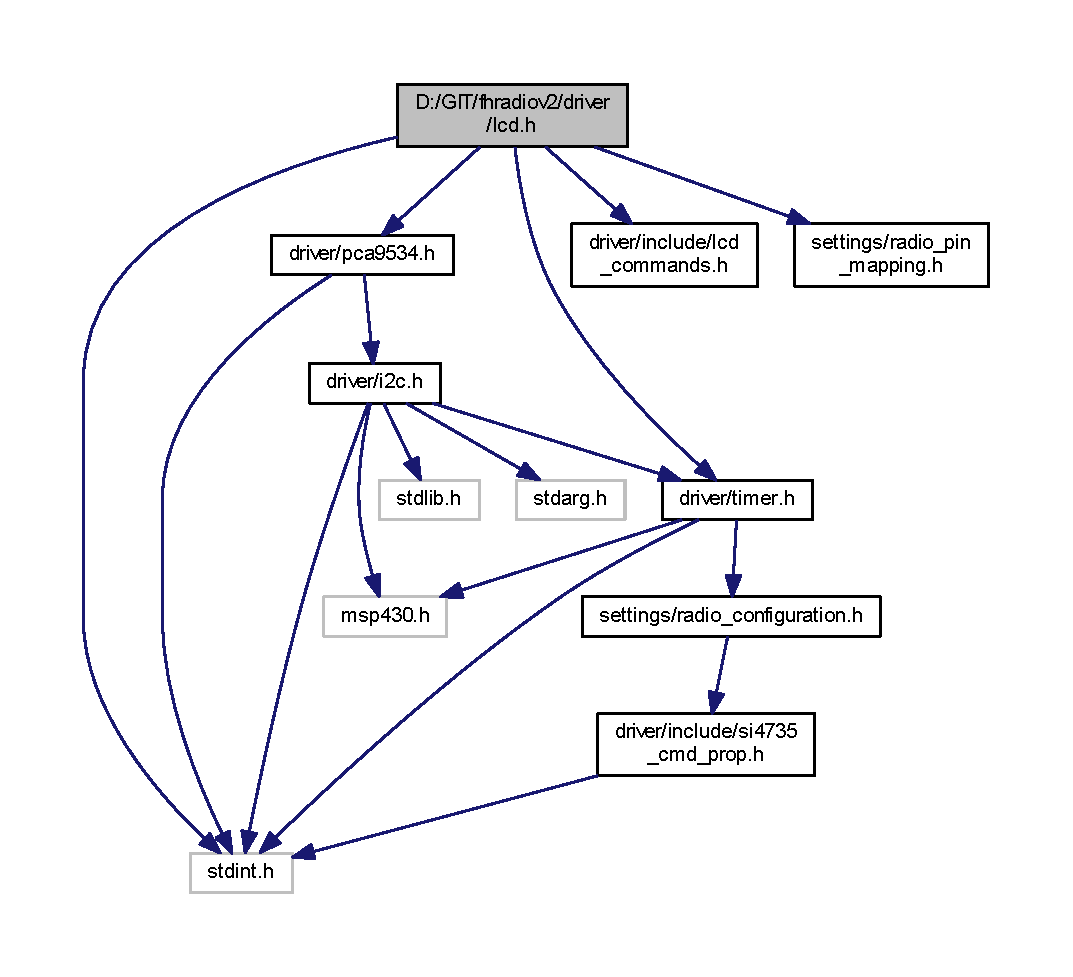
\includegraphics[width=350pt]{lcd_8h__incl}
\end{center}
\end{figure}
Dieser Graph zeigt, welche Datei direkt oder indirekt diese Datei enthält\+:\nopagebreak
\begin{figure}[H]
\begin{center}
\leavevmode
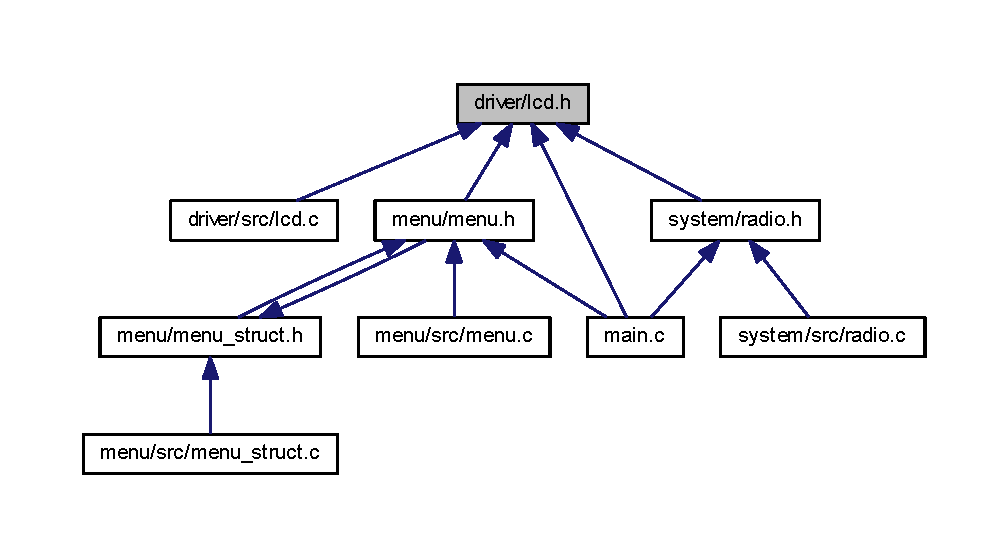
\includegraphics[width=350pt]{lcd_8h__dep__incl}
\end{center}
\end{figure}
\subsection*{Makrodefinitionen}
\begin{DoxyCompactItemize}
\item 
\#define \hyperlink{lcd_8h_a0092100866584e3511716fbf8e39c11f}{L\+C\+D\+\_\+\+E\+N\+A\+B\+L\+E\+\_\+\+H\+I\+G\+H}~0x10
\item 
\#define \hyperlink{lcd_8h_a0cbc0c73a8326693dcae8ceac5c7b71b}{L\+C\+D\+\_\+\+E\+N\+A\+B\+L\+E\+\_\+\+L\+O\+W}~0x00
\item 
\#define \hyperlink{lcd_8h_ad543004401896d9736084fcd833b7fd6}{L\+C\+D\+\_\+\+R\+E\+A\+D}~0x20
\item 
\#define \hyperlink{lcd_8h_ac83c798c669ca46b417ecc89c6ad37fe}{L\+C\+D\+\_\+\+W\+R\+I\+T\+E}~0x00
\item 
\#define \hyperlink{lcd_8h_a25e9d818788f36ed74d7c4579f87f2a6}{L\+C\+D\+\_\+\+D\+A\+T\+A}~0x40
\item 
\#define \hyperlink{lcd_8h_a28893b8aae31c65dfc6f5d478e225a2d}{L\+C\+D\+\_\+\+C\+M\+D}~0x00
\end{DoxyCompactItemize}
\subsection*{Funktionen}
\begin{DoxyCompactItemize}
\item 
uint8\+\_\+t \hyperlink{lcd_8h_a312eed1baec275e185dc00b760de1356}{lcd\+\_\+init} (uint8\+\_\+t contrast)
\item 
uint8\+\_\+t \hyperlink{lcd_8h_a011d26f08674b8430d53ea5e8cebd9e3}{lcd\+\_\+write\+\_\+char} (uint8\+\_\+t chr)
\item 
uint8\+\_\+t \hyperlink{lcd_8h_a2a4df97ebc5b396233aa31765228ef42}{lcd\+\_\+set\+\_\+courser} (uint8\+\_\+t x, uint8\+\_\+t y)
\item 
uint8\+\_\+t \hyperlink{lcd_8h_a41e4f70e7f07bd5333b929ed8f9df77f}{lcd\+\_\+command} (uint8\+\_\+t cmd)
\item 
uint8\+\_\+t \hyperlink{lcd_8h_a2e011676f64d2ee1c854b912133ae3f9}{lcd\+\_\+write\+\_\+string} (const int8\+\_\+t $\ast$str, uint8\+\_\+t n\+\_\+bytes)
\item 
uint8\+\_\+t \hyperlink{lcd_8h_a782f2bf84393a90f55c040d08c84b06d}{lcd\+\_\+connect} ()
\item 
uint8\+\_\+t \hyperlink{lcd_8h_ac5d817278ad99ea7420d6240c7e6cba6}{lcd\+\_\+generatechar} (uint8\+\_\+t code, const uint8\+\_\+t $\ast$data)
\item 
uint8\+\_\+t \hyperlink{lcd_8h_a737d0616c3643d82d1a612a5a667d709}{lcd\+\_\+bargraph} (uint8\+\_\+t value)
\item 
uint8\+\_\+t \hyperlink{lcd_8h_acd63fb85d212730fa4fcbcbeeccd231e}{lcd\+\_\+create\+\_\+view} (const char $\ast$str, uint8\+\_\+t x, uint8\+\_\+t y, uint8\+\_\+t num, uint8\+\_\+t flush)
\item 
uint8\+\_\+t \hyperlink{lcd_8h_ab99e48ab8689dcb1205c4c7c97bd9956}{lcd\+\_\+contrast} (uint8\+\_\+t contrast)
\item 
uint8\+\_\+t \hyperlink{lcd_8h_a6b9abf6cd27026b67144523ffbef4916}{lcd\+\_\+generatebargraph} ()
\end{DoxyCompactItemize}


\subsection{Makro-\/\+Dokumentation}
\hypertarget{lcd_8h_a28893b8aae31c65dfc6f5d478e225a2d}{}\index{lcd.\+h@{lcd.\+h}!L\+C\+D\+\_\+\+C\+M\+D@{L\+C\+D\+\_\+\+C\+M\+D}}
\index{L\+C\+D\+\_\+\+C\+M\+D@{L\+C\+D\+\_\+\+C\+M\+D}!lcd.\+h@{lcd.\+h}}
\subsubsection[{L\+C\+D\+\_\+\+C\+M\+D}]{\setlength{\rightskip}{0pt plus 5cm}\#define L\+C\+D\+\_\+\+C\+M\+D~0x00}\label{lcd_8h_a28893b8aae31c65dfc6f5d478e225a2d}


Definiert in Zeile 24 der Datei lcd.\+h.

\hypertarget{lcd_8h_a25e9d818788f36ed74d7c4579f87f2a6}{}\index{lcd.\+h@{lcd.\+h}!L\+C\+D\+\_\+\+D\+A\+T\+A@{L\+C\+D\+\_\+\+D\+A\+T\+A}}
\index{L\+C\+D\+\_\+\+D\+A\+T\+A@{L\+C\+D\+\_\+\+D\+A\+T\+A}!lcd.\+h@{lcd.\+h}}
\subsubsection[{L\+C\+D\+\_\+\+D\+A\+T\+A}]{\setlength{\rightskip}{0pt plus 5cm}\#define L\+C\+D\+\_\+\+D\+A\+T\+A~0x40}\label{lcd_8h_a25e9d818788f36ed74d7c4579f87f2a6}


Definiert in Zeile 23 der Datei lcd.\+h.

\hypertarget{lcd_8h_a0092100866584e3511716fbf8e39c11f}{}\index{lcd.\+h@{lcd.\+h}!L\+C\+D\+\_\+\+E\+N\+A\+B\+L\+E\+\_\+\+H\+I\+G\+H@{L\+C\+D\+\_\+\+E\+N\+A\+B\+L\+E\+\_\+\+H\+I\+G\+H}}
\index{L\+C\+D\+\_\+\+E\+N\+A\+B\+L\+E\+\_\+\+H\+I\+G\+H@{L\+C\+D\+\_\+\+E\+N\+A\+B\+L\+E\+\_\+\+H\+I\+G\+H}!lcd.\+h@{lcd.\+h}}
\subsubsection[{L\+C\+D\+\_\+\+E\+N\+A\+B\+L\+E\+\_\+\+H\+I\+G\+H}]{\setlength{\rightskip}{0pt plus 5cm}\#define L\+C\+D\+\_\+\+E\+N\+A\+B\+L\+E\+\_\+\+H\+I\+G\+H~0x10}\label{lcd_8h_a0092100866584e3511716fbf8e39c11f}


Definiert in Zeile 19 der Datei lcd.\+h.

\hypertarget{lcd_8h_a0cbc0c73a8326693dcae8ceac5c7b71b}{}\index{lcd.\+h@{lcd.\+h}!L\+C\+D\+\_\+\+E\+N\+A\+B\+L\+E\+\_\+\+L\+O\+W@{L\+C\+D\+\_\+\+E\+N\+A\+B\+L\+E\+\_\+\+L\+O\+W}}
\index{L\+C\+D\+\_\+\+E\+N\+A\+B\+L\+E\+\_\+\+L\+O\+W@{L\+C\+D\+\_\+\+E\+N\+A\+B\+L\+E\+\_\+\+L\+O\+W}!lcd.\+h@{lcd.\+h}}
\subsubsection[{L\+C\+D\+\_\+\+E\+N\+A\+B\+L\+E\+\_\+\+L\+O\+W}]{\setlength{\rightskip}{0pt plus 5cm}\#define L\+C\+D\+\_\+\+E\+N\+A\+B\+L\+E\+\_\+\+L\+O\+W~0x00}\label{lcd_8h_a0cbc0c73a8326693dcae8ceac5c7b71b}


Definiert in Zeile 20 der Datei lcd.\+h.

\hypertarget{lcd_8h_ad543004401896d9736084fcd833b7fd6}{}\index{lcd.\+h@{lcd.\+h}!L\+C\+D\+\_\+\+R\+E\+A\+D@{L\+C\+D\+\_\+\+R\+E\+A\+D}}
\index{L\+C\+D\+\_\+\+R\+E\+A\+D@{L\+C\+D\+\_\+\+R\+E\+A\+D}!lcd.\+h@{lcd.\+h}}
\subsubsection[{L\+C\+D\+\_\+\+R\+E\+A\+D}]{\setlength{\rightskip}{0pt plus 5cm}\#define L\+C\+D\+\_\+\+R\+E\+A\+D~0x20}\label{lcd_8h_ad543004401896d9736084fcd833b7fd6}


Definiert in Zeile 21 der Datei lcd.\+h.

\hypertarget{lcd_8h_ac83c798c669ca46b417ecc89c6ad37fe}{}\index{lcd.\+h@{lcd.\+h}!L\+C\+D\+\_\+\+W\+R\+I\+T\+E@{L\+C\+D\+\_\+\+W\+R\+I\+T\+E}}
\index{L\+C\+D\+\_\+\+W\+R\+I\+T\+E@{L\+C\+D\+\_\+\+W\+R\+I\+T\+E}!lcd.\+h@{lcd.\+h}}
\subsubsection[{L\+C\+D\+\_\+\+W\+R\+I\+T\+E}]{\setlength{\rightskip}{0pt plus 5cm}\#define L\+C\+D\+\_\+\+W\+R\+I\+T\+E~0x00}\label{lcd_8h_ac83c798c669ca46b417ecc89c6ad37fe}


Definiert in Zeile 22 der Datei lcd.\+h.



\subsection{Dokumentation der Funktionen}
\hypertarget{lcd_8h_a737d0616c3643d82d1a612a5a667d709}{}\index{lcd.\+h@{lcd.\+h}!lcd\+\_\+bargraph@{lcd\+\_\+bargraph}}
\index{lcd\+\_\+bargraph@{lcd\+\_\+bargraph}!lcd.\+h@{lcd.\+h}}
\subsubsection[{lcd\+\_\+bargraph}]{\setlength{\rightskip}{0pt plus 5cm}uint8\+\_\+t lcd\+\_\+bargraph (
\begin{DoxyParamCaption}
\item[{uint8\+\_\+t}]{value}
\end{DoxyParamCaption}
)}\label{lcd_8h_a737d0616c3643d82d1a612a5a667d709}
\hypertarget{lcd_8h_a41e4f70e7f07bd5333b929ed8f9df77f}{}\index{lcd.\+h@{lcd.\+h}!lcd\+\_\+command@{lcd\+\_\+command}}
\index{lcd\+\_\+command@{lcd\+\_\+command}!lcd.\+h@{lcd.\+h}}
\subsubsection[{lcd\+\_\+command}]{\setlength{\rightskip}{0pt plus 5cm}uint8\+\_\+t lcd\+\_\+command (
\begin{DoxyParamCaption}
\item[{uint8\+\_\+t}]{cmd}
\end{DoxyParamCaption}
)}\label{lcd_8h_a41e4f70e7f07bd5333b929ed8f9df77f}


Definiert in Zeile 150 der Datei lcd.\+c.


\begin{DoxyCode}
151 \{
152     \hyperlink{i2c_8h_a6691e5911f539e1e8178c6e983e8079a}{i2c\_write\_var}(\hyperlink{pca9534_8h_a327d2e2bdf4be4cf7155f21f093b9aae}{PCA9534\_I2C\_ADR}, \hyperlink{i2c_8h_aaaea3962492fd5ad1e43cba027d949d5a679ee5320d66c8322e310daeb2ee99b8}{STOP}, 1, ((command>>4) & 0x0f));
153     \hyperlink{timer_8c_a276d5cb665b9f8b2c79e53e2f2c5b4f0}{\_delay\_ms}(1);
154     \hyperlink{i2c_8h_a6691e5911f539e1e8178c6e983e8079a}{i2c\_write\_var}(\hyperlink{pca9534_8h_a327d2e2bdf4be4cf7155f21f093b9aae}{PCA9534\_I2C\_ADR}, \hyperlink{i2c_8h_aaaea3962492fd5ad1e43cba027d949d5a679ee5320d66c8322e310daeb2ee99b8}{STOP}, 1, (((command>>4) & 0x0f) | 0x10))
      ;
155     \hyperlink{timer_8c_a276d5cb665b9f8b2c79e53e2f2c5b4f0}{\_delay\_ms}(1);
156     \hyperlink{i2c_8h_a6691e5911f539e1e8178c6e983e8079a}{i2c\_write\_var}(\hyperlink{pca9534_8h_a327d2e2bdf4be4cf7155f21f093b9aae}{PCA9534\_I2C\_ADR}, \hyperlink{i2c_8h_aaaea3962492fd5ad1e43cba027d949d5a679ee5320d66c8322e310daeb2ee99b8}{STOP}, 1, (command & 0x0f));
157     \hyperlink{timer_8c_a276d5cb665b9f8b2c79e53e2f2c5b4f0}{\_delay\_ms}(1);
158     \hyperlink{i2c_8h_a6691e5911f539e1e8178c6e983e8079a}{i2c\_write\_var}(\hyperlink{pca9534_8h_a327d2e2bdf4be4cf7155f21f093b9aae}{PCA9534\_I2C\_ADR}, \hyperlink{i2c_8h_aaaea3962492fd5ad1e43cba027d949d5a679ee5320d66c8322e310daeb2ee99b8}{STOP}, 1, ((command & 0x0f) | 0x10));
159     \hyperlink{timer_8c_a276d5cb665b9f8b2c79e53e2f2c5b4f0}{\_delay\_ms}(5);
160     \textcolor{comment}{/*i2c\_write\_var(PCA9534\_I2C\_ADR, STOP, 2, 0x01, LCD\_HIGHER\_BYTE(command) | LCD\_ENABLE\_HIGH);}
161 \textcolor{comment}{    i2c\_write\_var(PCA9534\_I2C\_ADR, STOP, 2, 0x01, LCD\_HIGHER\_BYTE(command) | LCD\_ENABLE\_LOW);}
162 \textcolor{comment}{    i2c\_write\_var(PCA9534\_I2C\_ADR, STOP, 2, 0x01, LCD\_LOWER\_BYTE(command) | LCD\_ENABLE\_HIGH);}
163 \textcolor{comment}{    i2c\_write\_var(PCA9534\_I2C\_ADR, STOP, 2, 0x01, LCD\_LOWER\_BYTE(command) | LCD\_ENABLE\_LOW);*/}
164 
165     \textcolor{keywordflow}{return} 0;
166 \}
\end{DoxyCode}


Hier ist ein Graph, der zeigt, was diese Funktion aufruft\+:\nopagebreak
\begin{figure}[H]
\begin{center}
\leavevmode
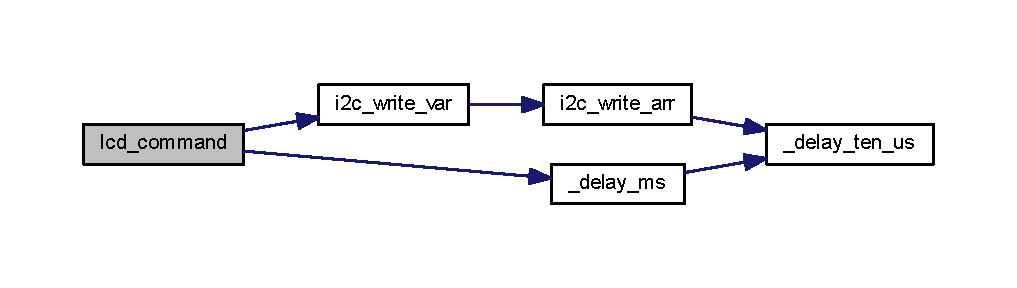
\includegraphics[width=350pt]{lcd_8h_a41e4f70e7f07bd5333b929ed8f9df77f_cgraph}
\end{center}
\end{figure}




Hier ist ein Graph der zeigt, wo diese Funktion aufgerufen wird\+:
\nopagebreak
\begin{figure}[H]
\begin{center}
\leavevmode
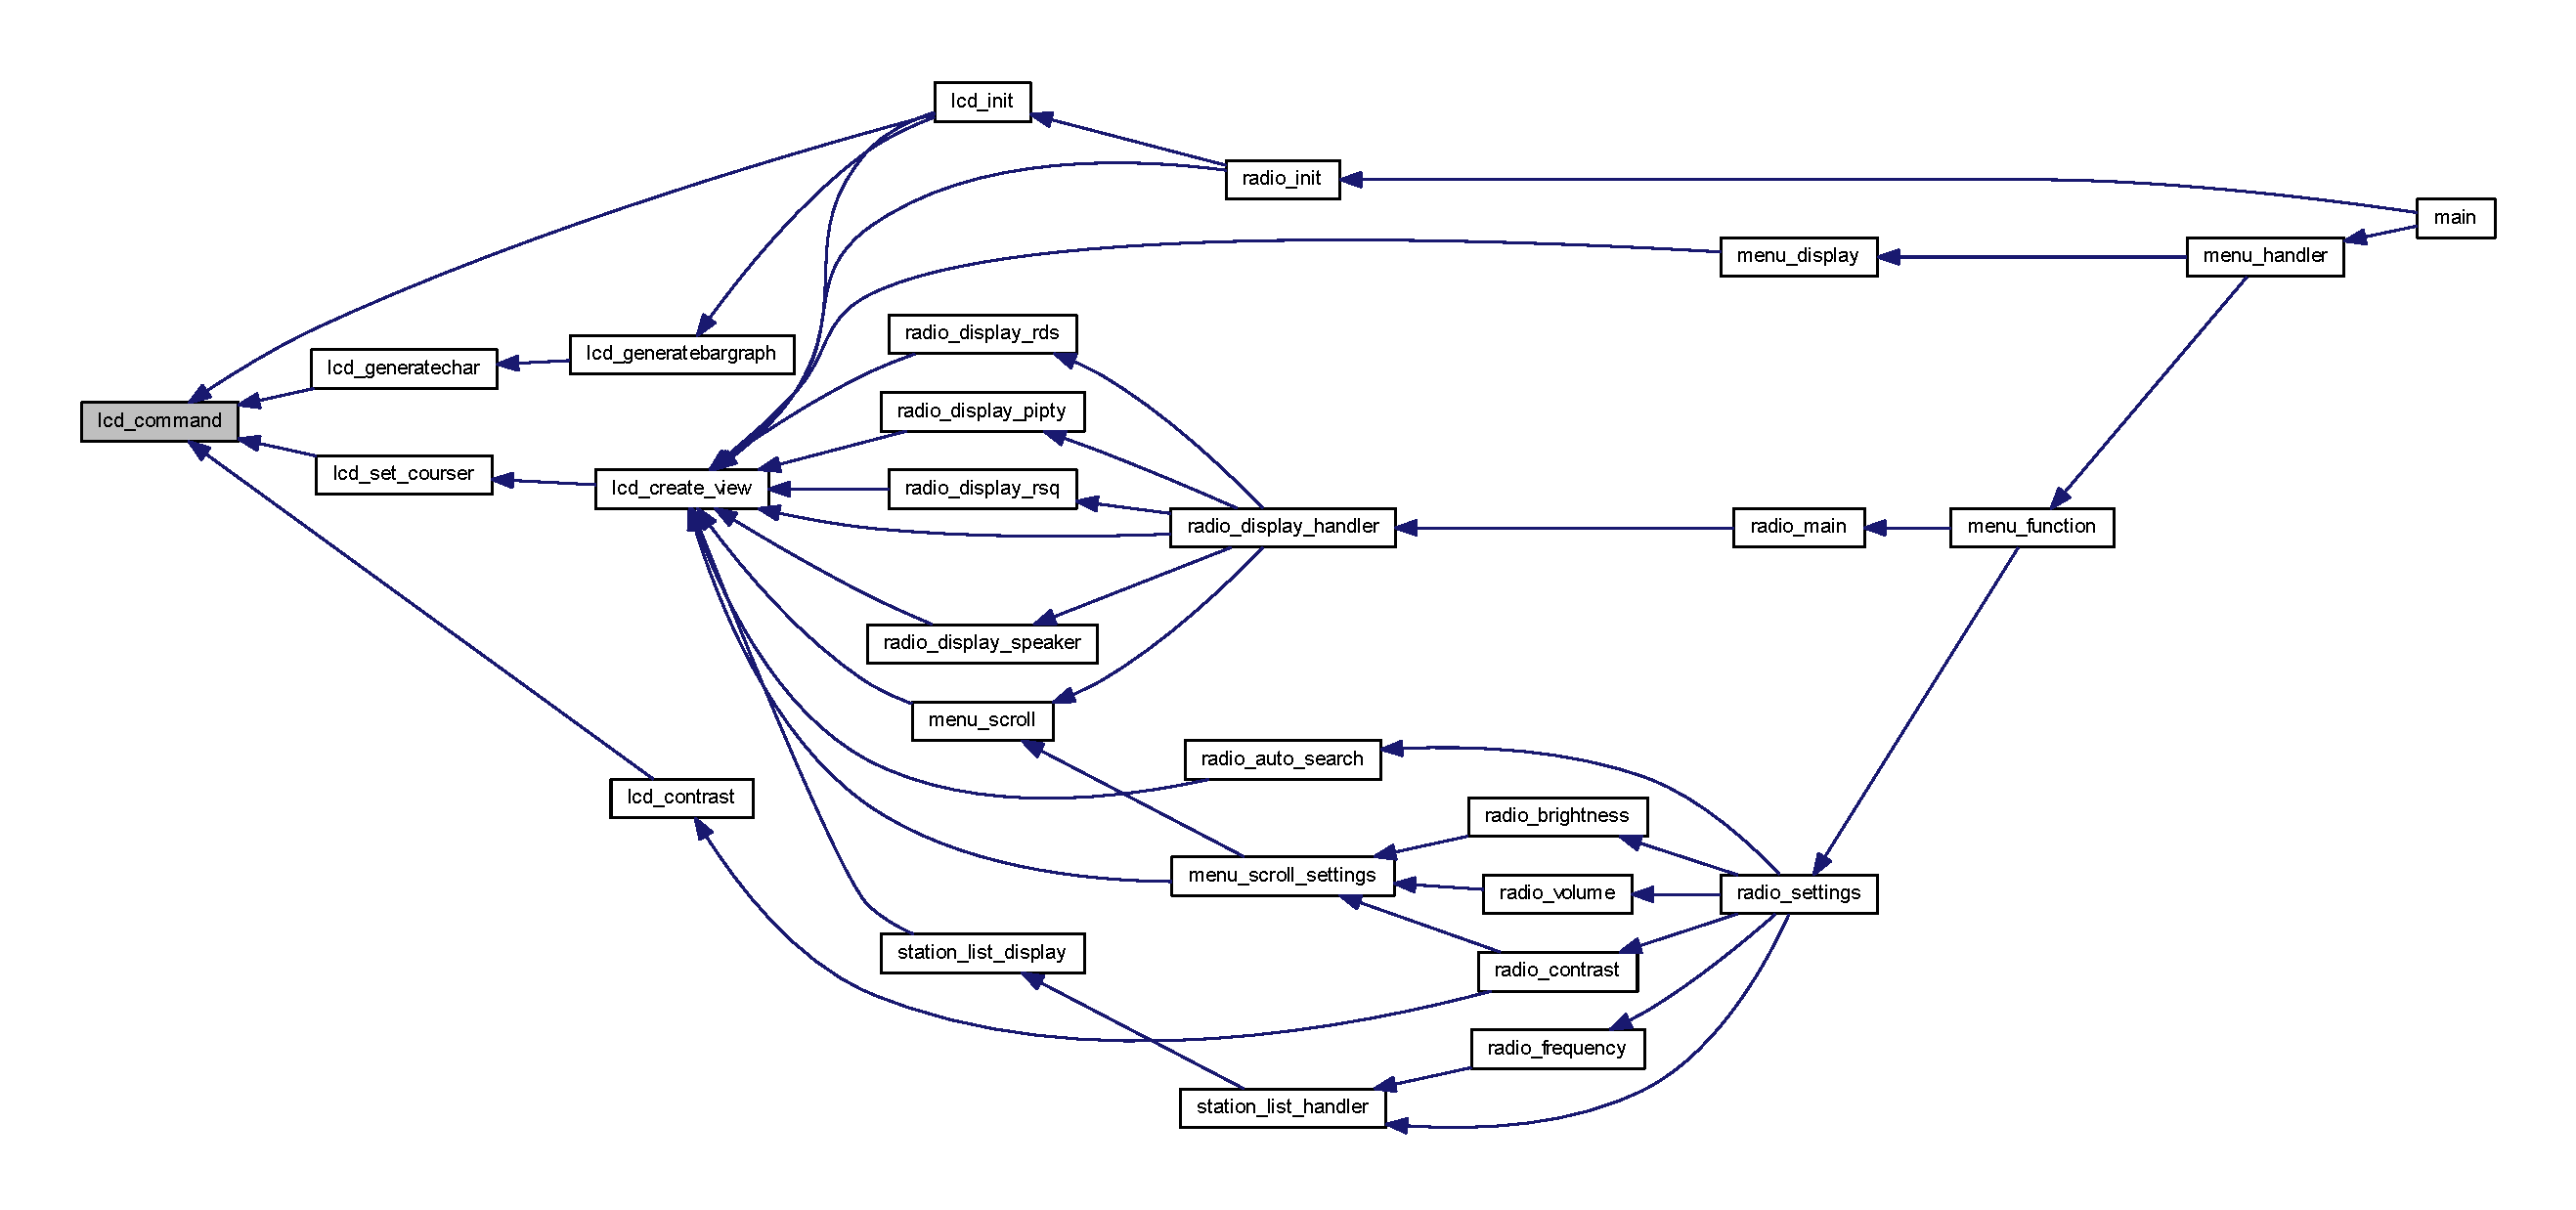
\includegraphics[width=350pt]{lcd_8h_a41e4f70e7f07bd5333b929ed8f9df77f_icgraph}
\end{center}
\end{figure}


\hypertarget{lcd_8h_a782f2bf84393a90f55c040d08c84b06d}{}\index{lcd.\+h@{lcd.\+h}!lcd\+\_\+connect@{lcd\+\_\+connect}}
\index{lcd\+\_\+connect@{lcd\+\_\+connect}!lcd.\+h@{lcd.\+h}}
\subsubsection[{lcd\+\_\+connect}]{\setlength{\rightskip}{0pt plus 5cm}uint8\+\_\+t lcd\+\_\+connect (
\begin{DoxyParamCaption}
{}
\end{DoxyParamCaption}
)}\label{lcd_8h_a782f2bf84393a90f55c040d08c84b06d}
\hypertarget{lcd_8h_ab99e48ab8689dcb1205c4c7c97bd9956}{}\index{lcd.\+h@{lcd.\+h}!lcd\+\_\+contrast@{lcd\+\_\+contrast}}
\index{lcd\+\_\+contrast@{lcd\+\_\+contrast}!lcd.\+h@{lcd.\+h}}
\subsubsection[{lcd\+\_\+contrast}]{\setlength{\rightskip}{0pt plus 5cm}uint8\+\_\+t lcd\+\_\+contrast (
\begin{DoxyParamCaption}
\item[{uint8\+\_\+t}]{contrast}
\end{DoxyParamCaption}
)}\label{lcd_8h_ab99e48ab8689dcb1205c4c7c97bd9956}


Definiert in Zeile 66 der Datei lcd.\+c.


\begin{DoxyCode}
67 \{
68     \hyperlink{lcd_8c_a250728451a22259562d3f01a12bbd77b}{lcd\_command}(\hyperlink{lcd__commands_8h_af8ec7e043a3b67ee423b97783d08aeb1}{LCD\_FUNCTION\_SET} | \hyperlink{lcd__commands_8h_add84145ade06b4f96934b7f1ed712e50}{LCD\_2\_LINE\_INST\_1});
69     \hyperlink{lcd_8c_a250728451a22259562d3f01a12bbd77b}{lcd\_command}(\hyperlink{lcd__commands_8h_a09afb8c9876350b83530222841b6b4ca}{LCD\_POWER\_CONTROL} | ((0x30 & contrast) >> 4));
70     \hyperlink{lcd_8c_a250728451a22259562d3f01a12bbd77b}{lcd\_command}(\hyperlink{lcd__commands_8h_a2dc0a014e84d69016cc4785bbc1fb3ac}{LCD\_CONTRAST\_SET} | (0x0F & contrast));
71     \hyperlink{lcd_8c_a250728451a22259562d3f01a12bbd77b}{lcd\_command}(\hyperlink{lcd__commands_8h_af8ec7e043a3b67ee423b97783d08aeb1}{LCD\_FUNCTION\_SET} | \hyperlink{lcd__commands_8h_a77febe1793148d377a47feafd8f00f2a}{LCD\_INST\_0});
72 
73     \textcolor{keywordflow}{return} 0;
74 \}
\end{DoxyCode}


Hier ist ein Graph, der zeigt, was diese Funktion aufruft\+:\nopagebreak
\begin{figure}[H]
\begin{center}
\leavevmode
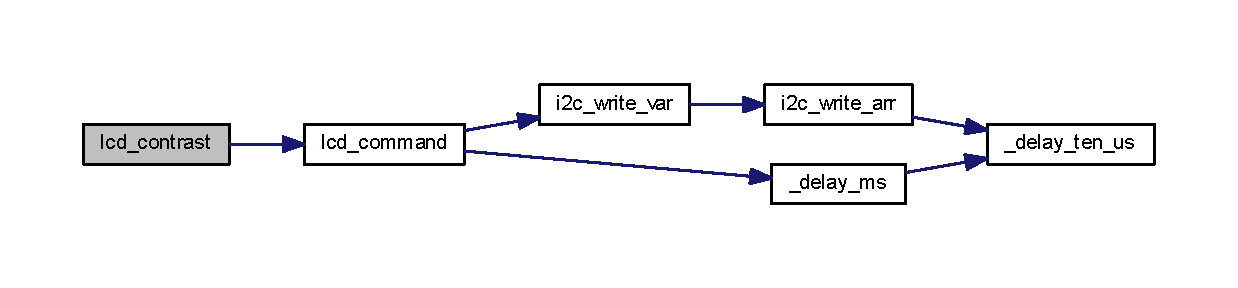
\includegraphics[width=350pt]{lcd_8h_ab99e48ab8689dcb1205c4c7c97bd9956_cgraph}
\end{center}
\end{figure}




Hier ist ein Graph der zeigt, wo diese Funktion aufgerufen wird\+:\nopagebreak
\begin{figure}[H]
\begin{center}
\leavevmode
\includegraphics[width=350pt]{lcd_8h_ab99e48ab8689dcb1205c4c7c97bd9956_icgraph}
\end{center}
\end{figure}


\hypertarget{lcd_8h_acd63fb85d212730fa4fcbcbeeccd231e}{}\index{lcd.\+h@{lcd.\+h}!lcd\+\_\+create\+\_\+view@{lcd\+\_\+create\+\_\+view}}
\index{lcd\+\_\+create\+\_\+view@{lcd\+\_\+create\+\_\+view}!lcd.\+h@{lcd.\+h}}
\subsubsection[{lcd\+\_\+create\+\_\+view}]{\setlength{\rightskip}{0pt plus 5cm}uint8\+\_\+t lcd\+\_\+create\+\_\+view (
\begin{DoxyParamCaption}
\item[{const char $\ast$}]{str, }
\item[{uint8\+\_\+t}]{x, }
\item[{uint8\+\_\+t}]{y, }
\item[{uint8\+\_\+t}]{num, }
\item[{uint8\+\_\+t}]{flush}
\end{DoxyParamCaption}
)}\label{lcd_8h_acd63fb85d212730fa4fcbcbeeccd231e}


Definiert in Zeile 315 der Datei lcd.\+c.


\begin{DoxyCode}
316 \{
317     \textcolor{keyword}{static} int8\_t lcd\_view[49];
318 
319     uint8\_t i,
320             pos;
321     \textcolor{comment}{/* invalid line position */}
322     \textcolor{keywordflow}{if} (x > 15) \{
323         \textcolor{keywordflow}{return} 0xFE;
324     \}
325 
326     \textcolor{comment}{/* invalid row position */}
327     \textcolor{keywordflow}{if} (y > 2) \{
328         \textcolor{keywordflow}{return} 0xFF;
329     \}
330 
331     pos = x + y * 16;
332 
333     \textcolor{keywordflow}{if}(num == 0) \{
334         num = 48;
335     \}
336 
337     \textcolor{comment}{/* if string is empty determinat string on given position */}
338     \textcolor{keywordflow}{if}(*str == 0 && num == 48) \{
339         lcd\_view[pos] = 0;
340     \}
341     \textcolor{keywordflow}{else} \{
342         \textcolor{comment}{/* copy string on given position */}
343         \textcolor{keywordflow}{while}(*str != 0 && pos < 48 && str != 0 && num > 0) \{\textcolor{comment}{//&& num > 0) \{}
344             lcd\_view[pos++] = *(str++);
345             num--;
346         \}
347     \}
348 
349     \textcolor{comment}{/* Normal flush with over writing lcd\_view with blanks */}
350     \textcolor{keywordflow}{if}(flush == 1) \{
351         \hyperlink{lcd_8c_a2a4df97ebc5b396233aa31765228ef42}{lcd\_set\_courser}(0,1);
352         \hyperlink{lcd_8c_aa6e1aa2ef9b677e16d8198df683429ec}{lcd\_write\_string}(lcd\_view,48);
353         \textcolor{keywordflow}{for}(i = 0; i < 48; i++) \{
354             lcd\_view[i] = \textcolor{charliteral}{' '};
355         \}
356         lcd\_view[48] = 0;
357     \}
358 
359     \textcolor{comment}{/* Init lcd\_view with blanks */}
360     \textcolor{keywordflow}{if}(flush == 2) \{
361         \textcolor{keywordflow}{for}(i = 0; i < 48; i++) \{
362             lcd\_view[i] = 0x20;
363         \}
364         lcd\_view[48] = 0;
365         \hyperlink{lcd_8c_a2a4df97ebc5b396233aa31765228ef42}{lcd\_set\_courser}(0,1);
366         \hyperlink{lcd_8c_aa6e1aa2ef9b677e16d8198df683429ec}{lcd\_write\_string}(lcd\_view,48);
367     \}
368 
369     \textcolor{keywordflow}{return} 0;
370 \}
\end{DoxyCode}


Hier ist ein Graph, der zeigt, was diese Funktion aufruft\+:\nopagebreak
\begin{figure}[H]
\begin{center}
\leavevmode
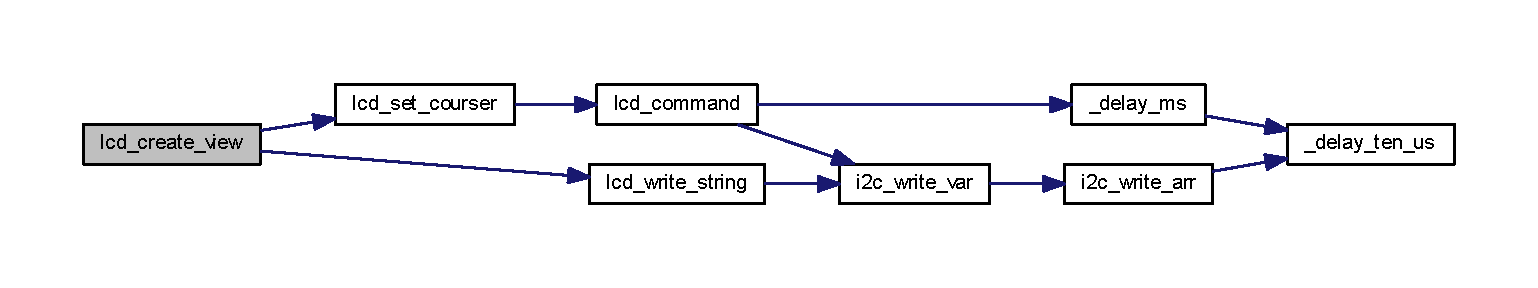
\includegraphics[width=350pt]{lcd_8h_acd63fb85d212730fa4fcbcbeeccd231e_cgraph}
\end{center}
\end{figure}




Hier ist ein Graph der zeigt, wo diese Funktion aufgerufen wird\+:
\nopagebreak
\begin{figure}[H]
\begin{center}
\leavevmode
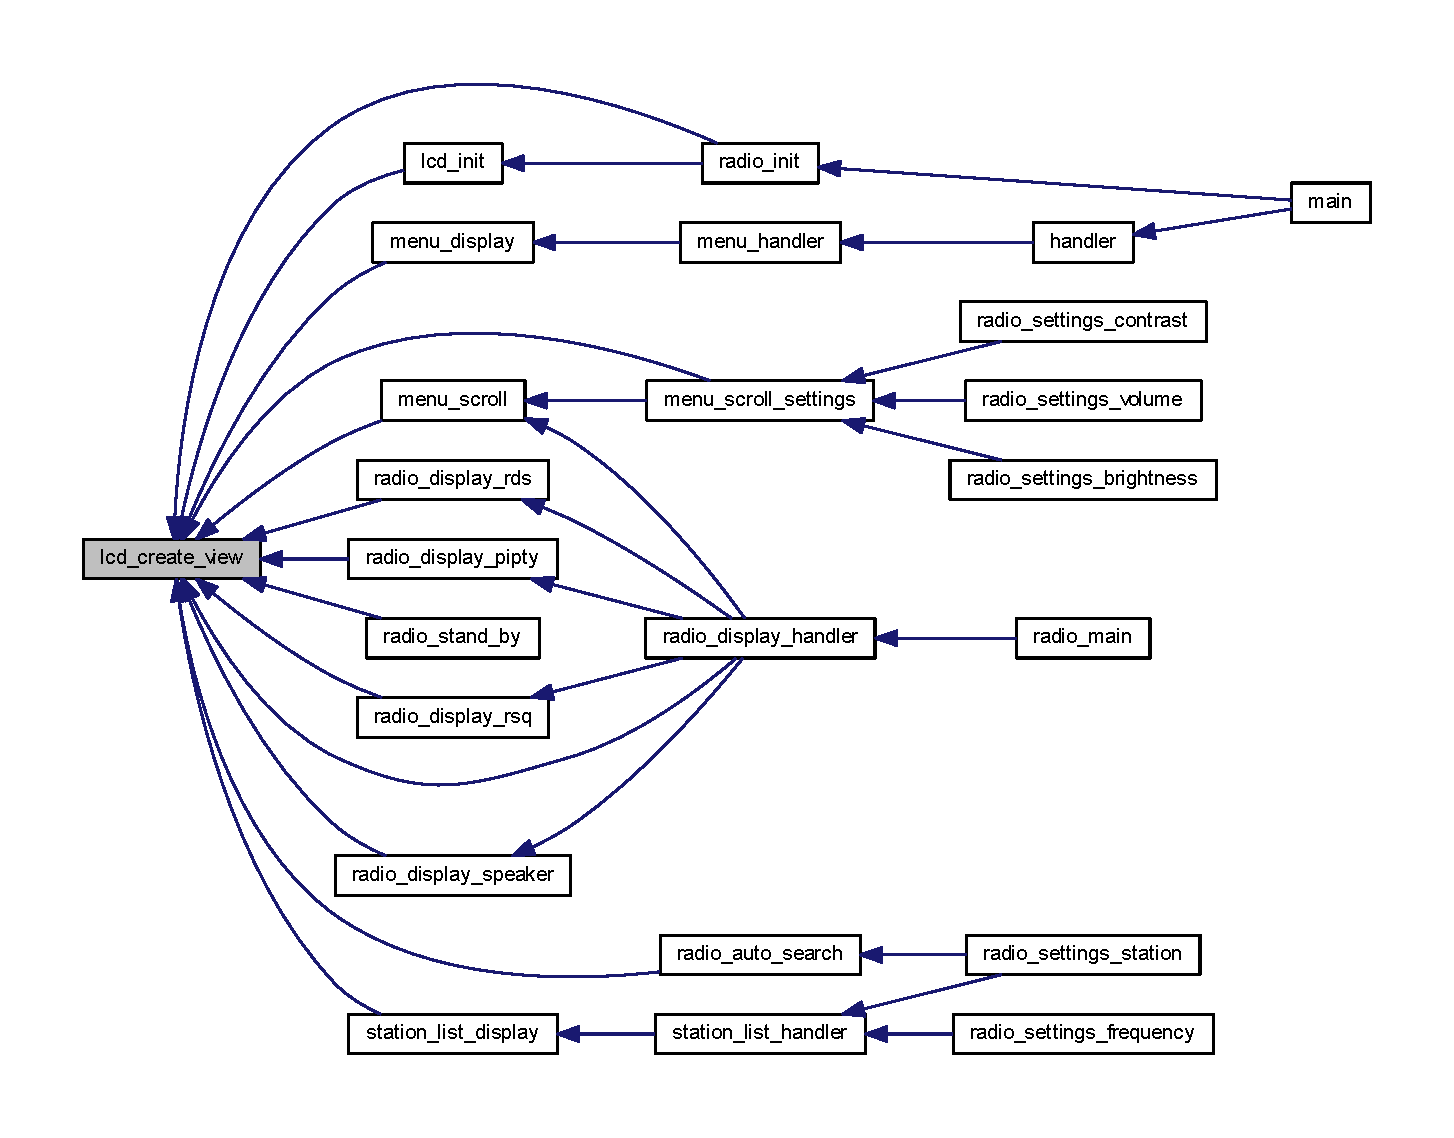
\includegraphics[width=350pt]{lcd_8h_acd63fb85d212730fa4fcbcbeeccd231e_icgraph}
\end{center}
\end{figure}


\hypertarget{lcd_8h_a6b9abf6cd27026b67144523ffbef4916}{}\index{lcd.\+h@{lcd.\+h}!lcd\+\_\+generatebargraph@{lcd\+\_\+generatebargraph}}
\index{lcd\+\_\+generatebargraph@{lcd\+\_\+generatebargraph}!lcd.\+h@{lcd.\+h}}
\subsubsection[{lcd\+\_\+generatebargraph}]{\setlength{\rightskip}{0pt plus 5cm}uint8\+\_\+t lcd\+\_\+generatebargraph (
\begin{DoxyParamCaption}
{}
\end{DoxyParamCaption}
)}\label{lcd_8h_a6b9abf6cd27026b67144523ffbef4916}


Definiert in Zeile 213 der Datei lcd.\+c.


\begin{DoxyCode}
214 \{
215     uint8\_t chrdata1[8] = \{
216         0x1F,   \textcolor{comment}{//xxxxx}
217         0x10,   \textcolor{comment}{//xoooo}
218         0x10,   \textcolor{comment}{//xoooo}
219         0x10,   \textcolor{comment}{//xoooo}
220         0x10,   \textcolor{comment}{//xoooo}
221         0x10,   \textcolor{comment}{//xoooo}
222         0x1F,   \textcolor{comment}{//xxxxx}
223         0x00
224     \};
225 
226     uint8\_t chrdata2[8] = \{
227         0x1F,   \textcolor{comment}{//xxxxx}
228         0x18,   \textcolor{comment}{//xxooo}
229         0x18,   \textcolor{comment}{//xxooo}
230         0x18,   \textcolor{comment}{//xxooo}
231         0x18,   \textcolor{comment}{//xxooo}
232         0x18,   \textcolor{comment}{//xxooo}
233         0x1F,   \textcolor{comment}{//xxxxx}
234         0x00
235     \};
236 
237     uint8\_t chrdata3[8] = \{
238         0x1F,   \textcolor{comment}{//xxxxx}
239         0x1C,   \textcolor{comment}{//xxxoo}
240         0x1C,   \textcolor{comment}{//xxxoo}
241         0x1C,   \textcolor{comment}{//xxxoo}
242         0x1C,   \textcolor{comment}{//xxxoo}
243         0x1C,   \textcolor{comment}{//xxxoo}
244         0x1F,   \textcolor{comment}{//xxxxx}
245         0x00
246     \};
247 
248     uint8\_t chrdata4[8] = \{
249         0x1F,   \textcolor{comment}{//xxxxx}
250         0x1E,   \textcolor{comment}{//xxxxo}
251         0x1E,   \textcolor{comment}{//xxxxo}
252         0x1E,   \textcolor{comment}{//xxxxo}
253         0x1E,   \textcolor{comment}{//xxxxo}
254         0x1E,   \textcolor{comment}{//xxxxo}
255         0x1F,   \textcolor{comment}{//xxxxx}
256         0x00
257     \};
258 
259     uint8\_t chrdata5[8] = \{
260         0x1F,   \textcolor{comment}{//xxxxx}
261         0x1F,   \textcolor{comment}{//xxxxx}
262         0x1F,   \textcolor{comment}{//xxxxx}
263         0x1F,   \textcolor{comment}{//xxxxx}
264         0x1F,   \textcolor{comment}{//xxxxx}
265         0x1F,   \textcolor{comment}{//xxxxx}
266         0x1F,   \textcolor{comment}{//xxxxx}
267         0x00
268     \};
269 
270     uint8\_t chrdata0[8] = \{
271         0x1F,   \textcolor{comment}{//xxxxx}
272         0x00,   \textcolor{comment}{//ooooo}
273         0x00,   \textcolor{comment}{//ooooo}
274         0x00,   \textcolor{comment}{//ooooo}
275         0x00,   \textcolor{comment}{//ooooo}
276         0x00,   \textcolor{comment}{//ooooo}
277         0x1F,   \textcolor{comment}{//xxxxx}
278         0x00
279     \};
280 
281     uint8\_t chrdata6[8] = \{
282         0x0E,   \textcolor{comment}{//oxxxo}
283         0x15,   \textcolor{comment}{//xoxox}
284         0x15,   \textcolor{comment}{//xoxox}
285         0x17,   \textcolor{comment}{//xoxxx}
286         0x11,   \textcolor{comment}{//oooox}
287         0x11,   \textcolor{comment}{//xooox}
288         0x0E,   \textcolor{comment}{//oxxxo}
289         0x00
290     \};
291 
292     uint8\_t chrdata7[8] = \{
293         0x03,   \textcolor{comment}{//oooxx}
294         0x05,   \textcolor{comment}{//ooxox}
295         0x19,   \textcolor{comment}{//xxoox}
296         0x11,   \textcolor{comment}{//xxoox}
297         0x19,   \textcolor{comment}{//xxoox}
298         0x05,   \textcolor{comment}{//ooxox}
299         0x03,   \textcolor{comment}{//oooxx}
300         0x00
301     \};
302 
303     \hyperlink{lcd_8c_ac5d817278ad99ea7420d6240c7e6cba6}{lcd\_generatechar}(0,chrdata0);
304     \hyperlink{lcd_8c_ac5d817278ad99ea7420d6240c7e6cba6}{lcd\_generatechar}(1,chrdata1);
305     \hyperlink{lcd_8c_ac5d817278ad99ea7420d6240c7e6cba6}{lcd\_generatechar}(2,chrdata2);
306     \hyperlink{lcd_8c_ac5d817278ad99ea7420d6240c7e6cba6}{lcd\_generatechar}(3,chrdata3);
307     \hyperlink{lcd_8c_ac5d817278ad99ea7420d6240c7e6cba6}{lcd\_generatechar}(4,chrdata4);
308     \hyperlink{lcd_8c_ac5d817278ad99ea7420d6240c7e6cba6}{lcd\_generatechar}(5,chrdata5);
309     \hyperlink{lcd_8c_ac5d817278ad99ea7420d6240c7e6cba6}{lcd\_generatechar}(6,chrdata6);
310     \hyperlink{lcd_8c_ac5d817278ad99ea7420d6240c7e6cba6}{lcd\_generatechar}(7,chrdata7);
311 
312     \textcolor{keywordflow}{return} 0;
313 \}
\end{DoxyCode}


Hier ist ein Graph, der zeigt, was diese Funktion aufruft\+:\nopagebreak
\begin{figure}[H]
\begin{center}
\leavevmode
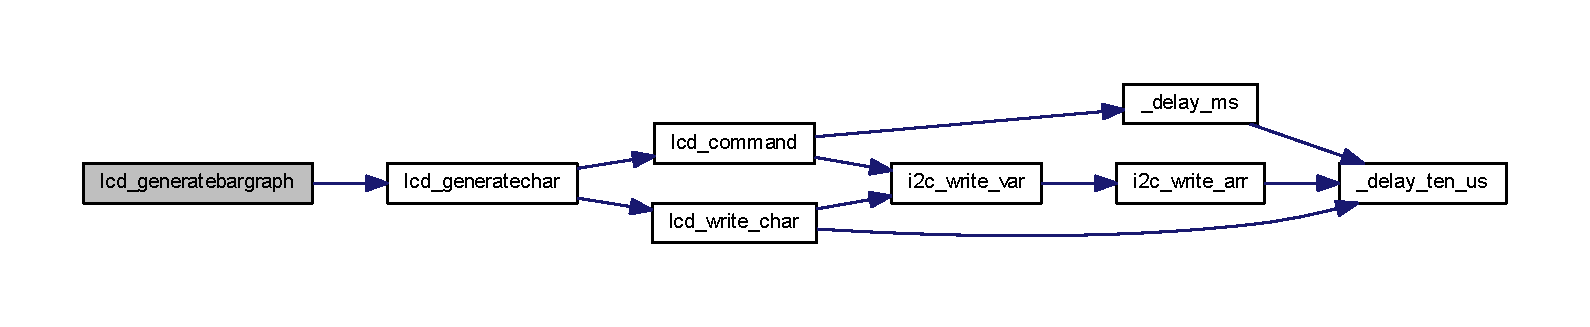
\includegraphics[width=350pt]{lcd_8h_a6b9abf6cd27026b67144523ffbef4916_cgraph}
\end{center}
\end{figure}




Hier ist ein Graph der zeigt, wo diese Funktion aufgerufen wird\+:\nopagebreak
\begin{figure}[H]
\begin{center}
\leavevmode
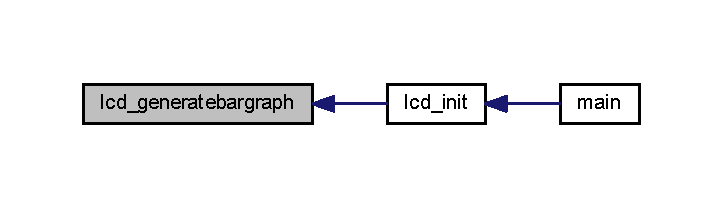
\includegraphics[width=350pt]{lcd_8h_a6b9abf6cd27026b67144523ffbef4916_icgraph}
\end{center}
\end{figure}


\hypertarget{lcd_8h_ac5d817278ad99ea7420d6240c7e6cba6}{}\index{lcd.\+h@{lcd.\+h}!lcd\+\_\+generatechar@{lcd\+\_\+generatechar}}
\index{lcd\+\_\+generatechar@{lcd\+\_\+generatechar}!lcd.\+h@{lcd.\+h}}
\subsubsection[{lcd\+\_\+generatechar}]{\setlength{\rightskip}{0pt plus 5cm}uint8\+\_\+t lcd\+\_\+generatechar (
\begin{DoxyParamCaption}
\item[{uint8\+\_\+t}]{code, }
\item[{const uint8\+\_\+t $\ast$}]{data}
\end{DoxyParamCaption}
)}\label{lcd_8h_ac5d817278ad99ea7420d6240c7e6cba6}


Definiert in Zeile 198 der Datei lcd.\+c.


\begin{DoxyCode}
199 \{
200     uint8\_t i = 0;
201     \textcolor{comment}{// Startposition des Zeichens einstellen}
202     \hyperlink{lcd_8c_a250728451a22259562d3f01a12bbd77b}{lcd\_command}(\hyperlink{lcd__commands_8h_a5109f670d7f397ba8845d08167bf4ab2}{LCD\_SET\_CGADR}|(code<<3));
203 
204     \textcolor{comment}{// Bitmuster �bertragen}
205     \textcolor{keywordflow}{for} (i = 0; i < 8; i++)
206     \{
207         \hyperlink{lcd_8c_a1a22a2c5cd6e0e4e06977a2f78a7ab08}{lcd\_write\_char}(data[i]);
208     \}
209 
210     \textcolor{keywordflow}{return} 0;
211 \}
\end{DoxyCode}


Hier ist ein Graph, der zeigt, was diese Funktion aufruft\+:\nopagebreak
\begin{figure}[H]
\begin{center}
\leavevmode
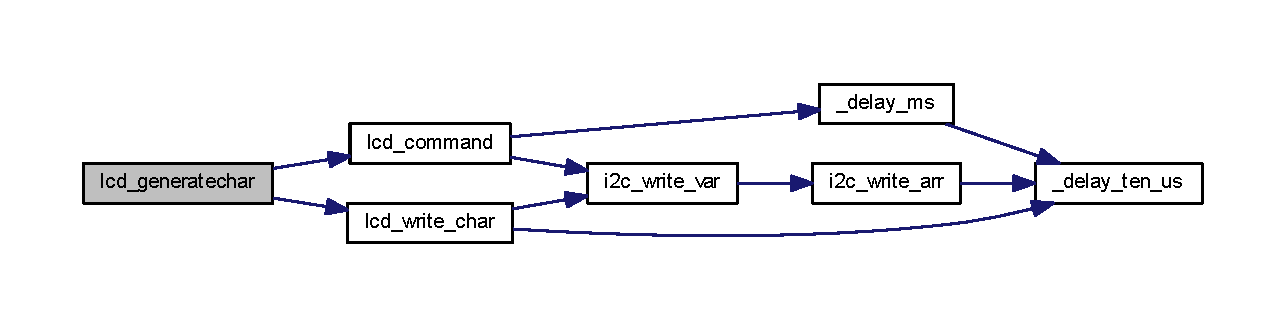
\includegraphics[width=350pt]{lcd_8h_ac5d817278ad99ea7420d6240c7e6cba6_cgraph}
\end{center}
\end{figure}




Hier ist ein Graph der zeigt, wo diese Funktion aufgerufen wird\+:\nopagebreak
\begin{figure}[H]
\begin{center}
\leavevmode
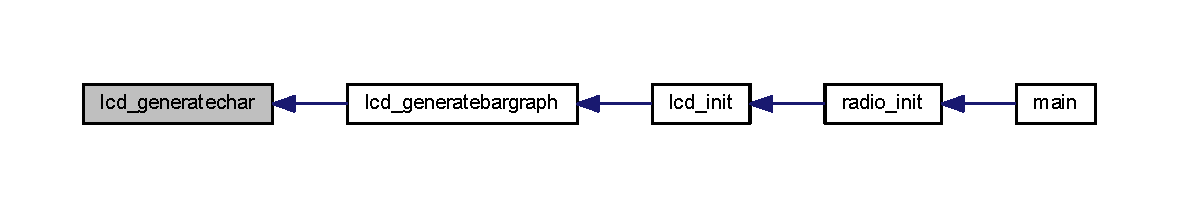
\includegraphics[width=350pt]{lcd_8h_ac5d817278ad99ea7420d6240c7e6cba6_icgraph}
\end{center}
\end{figure}


\hypertarget{lcd_8h_a312eed1baec275e185dc00b760de1356}{}\index{lcd.\+h@{lcd.\+h}!lcd\+\_\+init@{lcd\+\_\+init}}
\index{lcd\+\_\+init@{lcd\+\_\+init}!lcd.\+h@{lcd.\+h}}
\subsubsection[{lcd\+\_\+init}]{\setlength{\rightskip}{0pt plus 5cm}uint8\+\_\+t lcd\+\_\+init (
\begin{DoxyParamCaption}
\item[{uint8\+\_\+t}]{contrast}
\end{DoxyParamCaption}
)}\label{lcd_8h_a312eed1baec275e185dc00b760de1356}


Definiert in Zeile 12 der Datei lcd.\+c.


\begin{DoxyCode}
13 \{
14 
15     \textcolor{comment}{// Activate PCA9534}
16     \hyperlink{radio__pin__mapping_8h_a131b17b16bb25a95f17f81423722dcb1}{PCA\_ON\_OFF\_SEL} &= (~\hyperlink{radio__pin__mapping_8h_a24dbe611147513e518aaa1b1034e19d9}{PCA\_ON\_OFF\_PIN});
17     \hyperlink{radio__pin__mapping_8h_aca9911d61d5202bad563d5f748782548}{PCA\_ON\_OFF\_DIR} |= \hyperlink{radio__pin__mapping_8h_a24dbe611147513e518aaa1b1034e19d9}{PCA\_ON\_OFF\_PIN};
18     \hyperlink{radio__pin__mapping_8h_abd6e55737a7d5e65b8582d647b103f8e}{PCA\_ON\_OFF\_OUT} |= \hyperlink{radio__pin__mapping_8h_a24dbe611147513e518aaa1b1034e19d9}{PCA\_ON\_OFF\_PIN};
19 
20 
21     \textcolor{comment}{// Go in default state}
22     \textcolor{comment}{//pca9534\_config(0x7F);}
23 
24     \textcolor{comment}{//i2c\_write\_var(PCA9534\_I2C\_ADR, STOP, 2,0x03, 0x00);}
25 
26     \hyperlink{timer_8c_a276d5cb665b9f8b2c79e53e2f2c5b4f0}{\_delay\_ms}(100);
27 
28     \textcolor{comment}{// Send reset command}
29     \hyperlink{i2c_8h_a6691e5911f539e1e8178c6e983e8079a}{i2c\_write\_var}(\hyperlink{pca9534_8h_a327d2e2bdf4be4cf7155f21f093b9aae}{PCA9534\_I2C\_ADR}, \hyperlink{i2c_8h_aaaea3962492fd5ad1e43cba027d949d5a679ee5320d66c8322e310daeb2ee99b8}{STOP}, 2, 0x03, 0x13);
30 
31     \hyperlink{timer_8c_a276d5cb665b9f8b2c79e53e2f2c5b4f0}{\_delay\_ms}(2);
32 
33     \textcolor{comment}{// Send 2nd reset command}
34     \hyperlink{i2c_8h_a6691e5911f539e1e8178c6e983e8079a}{i2c\_write\_var}(\hyperlink{pca9534_8h_a327d2e2bdf4be4cf7155f21f093b9aae}{PCA9534\_I2C\_ADR}, \hyperlink{i2c_8h_aaaea3962492fd5ad1e43cba027d949d5a679ee5320d66c8322e310daeb2ee99b8}{STOP}, 2, 0x03, 0x13);
35 
36     \hyperlink{timer_8c_a3c56af3315c2461dec5ced585a5f84db}{\_delay\_ten\_us}(3);
37 
38     \textcolor{comment}{// Send 3rd reset command}
39     \hyperlink{i2c_8h_a6691e5911f539e1e8178c6e983e8079a}{i2c\_write\_var}(\hyperlink{pca9534_8h_a327d2e2bdf4be4cf7155f21f093b9aae}{PCA9534\_I2C\_ADR}, \hyperlink{i2c_8h_aaaea3962492fd5ad1e43cba027d949d5a679ee5320d66c8322e310daeb2ee99b8}{STOP}, 2, 0x03, 0x13);
40 
41     \textcolor{comment}{// Go in default data mode of display}
42     \hyperlink{i2c_8h_a6691e5911f539e1e8178c6e983e8079a}{i2c\_write\_var}(\hyperlink{pca9534_8h_a327d2e2bdf4be4cf7155f21f093b9aae}{PCA9534\_I2C\_ADR}, \hyperlink{i2c_8h_aaaea3962492fd5ad1e43cba027d949d5a679ee5320d66c8322e310daeb2ee99b8}{STOP}, 2, 0x02, 0x12);
43 
44     \hyperlink{timer_8c_a3c56af3315c2461dec5ced585a5f84db}{\_delay\_ten\_us}(3);
45 
46     \hyperlink{lcd_8c_a250728451a22259562d3f01a12bbd77b}{lcd\_command}(\hyperlink{lcd__commands_8h_af8ec7e043a3b67ee423b97783d08aeb1}{LCD\_FUNCTION\_SET} | \hyperlink{lcd__commands_8h_add84145ade06b4f96934b7f1ed712e50}{LCD\_2\_LINE\_INST\_1});
47     \hyperlink{lcd_8c_a250728451a22259562d3f01a12bbd77b}{lcd\_command}(\hyperlink{lcd__commands_8h_aa16d1fe8c9651f81c3f1649e57bc870c}{LCD\_BIAS\_SET} | \hyperlink{lcd__commands_8h_a3e0a4be625c4ed54cf0257a3b526ea00}{LCD\_BIAS\_1\_4} | 
      \hyperlink{lcd__commands_8h_af685b6108573c92216437b1a512c6a72}{LCD\_3\_LINE});
48     \hyperlink{lcd_8c_a250728451a22259562d3f01a12bbd77b}{lcd\_command}(\hyperlink{lcd__commands_8h_a09afb8c9876350b83530222841b6b4ca}{LCD\_POWER\_CONTROL} | ((0x30 & contrast) >> 4));
49     \hyperlink{lcd_8c_a250728451a22259562d3f01a12bbd77b}{lcd\_command}(\hyperlink{lcd__commands_8h_aa182b257140f187c7ceb85761802a6d4}{LCD\_FOLLOWER\_CONTROL} | 
      \hyperlink{lcd__commands_8h_aa7170591c5c6954165b8f1b6c94bdcea}{LCD\_FOLLOWER\_CIRCUT\_ON} | \hyperlink{lcd__commands_8h_af05126b3001c839af73fdbc7e2b0940e}{LCD\_AMPLIFFED\_RATIO});
50     \hyperlink{lcd_8c_a250728451a22259562d3f01a12bbd77b}{lcd\_command}(\hyperlink{lcd__commands_8h_a2dc0a014e84d69016cc4785bbc1fb3ac}{LCD\_CONTRAST\_SET} | (0x0F & contrast));
51     \hyperlink{lcd_8c_a250728451a22259562d3f01a12bbd77b}{lcd\_command}(\hyperlink{lcd__commands_8h_af8ec7e043a3b67ee423b97783d08aeb1}{LCD\_FUNCTION\_SET} | \hyperlink{lcd__commands_8h_a77febe1793148d377a47feafd8f00f2a}{LCD\_INST\_0});
52     \hyperlink{lcd_8c_a250728451a22259562d3f01a12bbd77b}{lcd\_command}(\hyperlink{lcd__commands_8h_a9b4eda8a777de7cc4b7cbaa71621029e}{LCD\_DISPLAY\_CONTROL} | 
      \hyperlink{lcd__commands_8h_a846dac5d1bb72bef7a76ee110c0445b6}{LCD\_DISPLAY\_ON});
53     \hyperlink{lcd_8c_a250728451a22259562d3f01a12bbd77b}{lcd\_command}(\hyperlink{lcd__commands_8h_ac547b969070db1798702062faca30c6e}{LCD\_CLEAR\_SCREEN});
54     \hyperlink{lcd_8c_a250728451a22259562d3f01a12bbd77b}{lcd\_command}(\hyperlink{lcd__commands_8h_ae5e77a91b0fef0c36af29424a1ee2da1}{LCD\_ENTRY\_MODE\_SET} | 
      \hyperlink{lcd__commands_8h_a6e5a50c1f9f21c012e6d44ebcd5fd65f}{LCD\_COURSER\_INKREMENT});
55     \hyperlink{lcd_8c_a250728451a22259562d3f01a12bbd77b}{lcd\_command}(\hyperlink{lcd__commands_8h_a350fda109811fb23bfaf6ef763c31b9b}{LCD\_RESET\_COURSER});
56 
57     \textcolor{comment}{//Gernarte GCCR Symbole}
58     \hyperlink{lcd_8c_a6b9abf6cd27026b67144523ffbef4916}{lcd\_generatebargraph}();
59 
60     \textcolor{comment}{//Clear LCD and Init view ram}
61     \hyperlink{lcd_8c_acd63fb85d212730fa4fcbcbeeccd231e}{lcd\_create\_view}(0, 0, 0, 0, 2);
62 
63     \textcolor{keywordflow}{return} 0;
64 \}
\end{DoxyCode}


Hier ist ein Graph, der zeigt, was diese Funktion aufruft\+:\nopagebreak
\begin{figure}[H]
\begin{center}
\leavevmode
\includegraphics[width=350pt]{lcd_8h_a312eed1baec275e185dc00b760de1356_cgraph}
\end{center}
\end{figure}




Hier ist ein Graph der zeigt, wo diese Funktion aufgerufen wird\+:\nopagebreak
\begin{figure}[H]
\begin{center}
\leavevmode
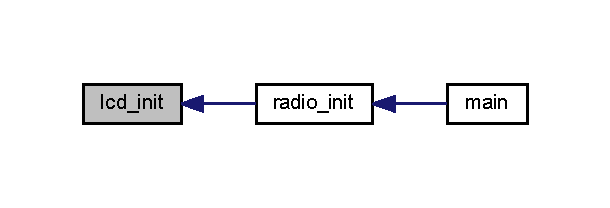
\includegraphics[width=293pt]{lcd_8h_a312eed1baec275e185dc00b760de1356_icgraph}
\end{center}
\end{figure}


\hypertarget{lcd_8h_a2a4df97ebc5b396233aa31765228ef42}{}\index{lcd.\+h@{lcd.\+h}!lcd\+\_\+set\+\_\+courser@{lcd\+\_\+set\+\_\+courser}}
\index{lcd\+\_\+set\+\_\+courser@{lcd\+\_\+set\+\_\+courser}!lcd.\+h@{lcd.\+h}}
\subsubsection[{lcd\+\_\+set\+\_\+courser}]{\setlength{\rightskip}{0pt plus 5cm}uint8\+\_\+t lcd\+\_\+set\+\_\+courser (
\begin{DoxyParamCaption}
\item[{uint8\+\_\+t}]{x, }
\item[{uint8\+\_\+t}]{y}
\end{DoxyParamCaption}
)}\label{lcd_8h_a2a4df97ebc5b396233aa31765228ef42}


Definiert in Zeile 173 der Datei lcd.\+c.


\begin{DoxyCode}
174 \{
175     \textcolor{keywordflow}{if} (x > 15) \{
176         \textcolor{keywordflow}{return} 0xFE;
177     \}
178 
179     \textcolor{keywordflow}{switch} (y) \{
180         \textcolor{keywordflow}{case} 1:
181             \hyperlink{lcd_8c_a250728451a22259562d3f01a12bbd77b}{lcd\_command}(x + \hyperlink{lcd__commands_8h_ad3c37e4453c7f7ba2d5220f9d8fa8502}{LCD\_ADRESS\_LINE\_1});
182             \textcolor{keywordflow}{break};
183         \textcolor{keywordflow}{case} 2:
184             \hyperlink{lcd_8c_a250728451a22259562d3f01a12bbd77b}{lcd\_command}(x + \hyperlink{lcd__commands_8h_a357f0824fb224d0925d6ca5230585814}{LCD\_ADRESS\_LINE\_2});
185             \textcolor{keywordflow}{break};
186         \textcolor{keywordflow}{case} 3:
187             \hyperlink{lcd_8c_a250728451a22259562d3f01a12bbd77b}{lcd\_command}(x + \hyperlink{lcd__commands_8h_a0531c4c867eea2495519880aecd7c422}{LCD\_ADRESS\_LINE\_3});
188             \textcolor{keywordflow}{break};
189         \textcolor{keywordflow}{case} 4:
190             \hyperlink{lcd_8c_a250728451a22259562d3f01a12bbd77b}{lcd\_command}(x + \hyperlink{lcd__commands_8h_a467510be8265e0cc87ce3e4110f9e75e}{LCD\_ADRESS\_LINE\_4});
191             \textcolor{keywordflow}{break};
192         \textcolor{keywordflow}{default}:
193             \textcolor{keywordflow}{return} 0xFF;
194     \}
195     \textcolor{keywordflow}{return} 0;
196 \}
\end{DoxyCode}


Hier ist ein Graph, der zeigt, was diese Funktion aufruft\+:\nopagebreak
\begin{figure}[H]
\begin{center}
\leavevmode
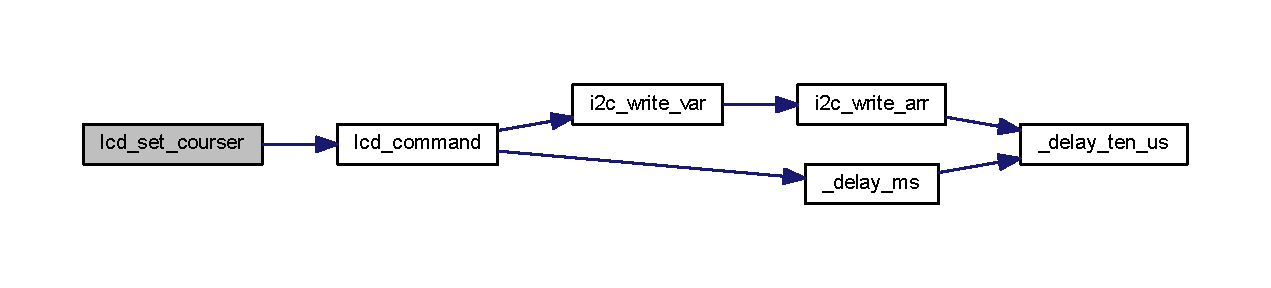
\includegraphics[width=350pt]{lcd_8h_a2a4df97ebc5b396233aa31765228ef42_cgraph}
\end{center}
\end{figure}




Hier ist ein Graph der zeigt, wo diese Funktion aufgerufen wird\+:
\nopagebreak
\begin{figure}[H]
\begin{center}
\leavevmode
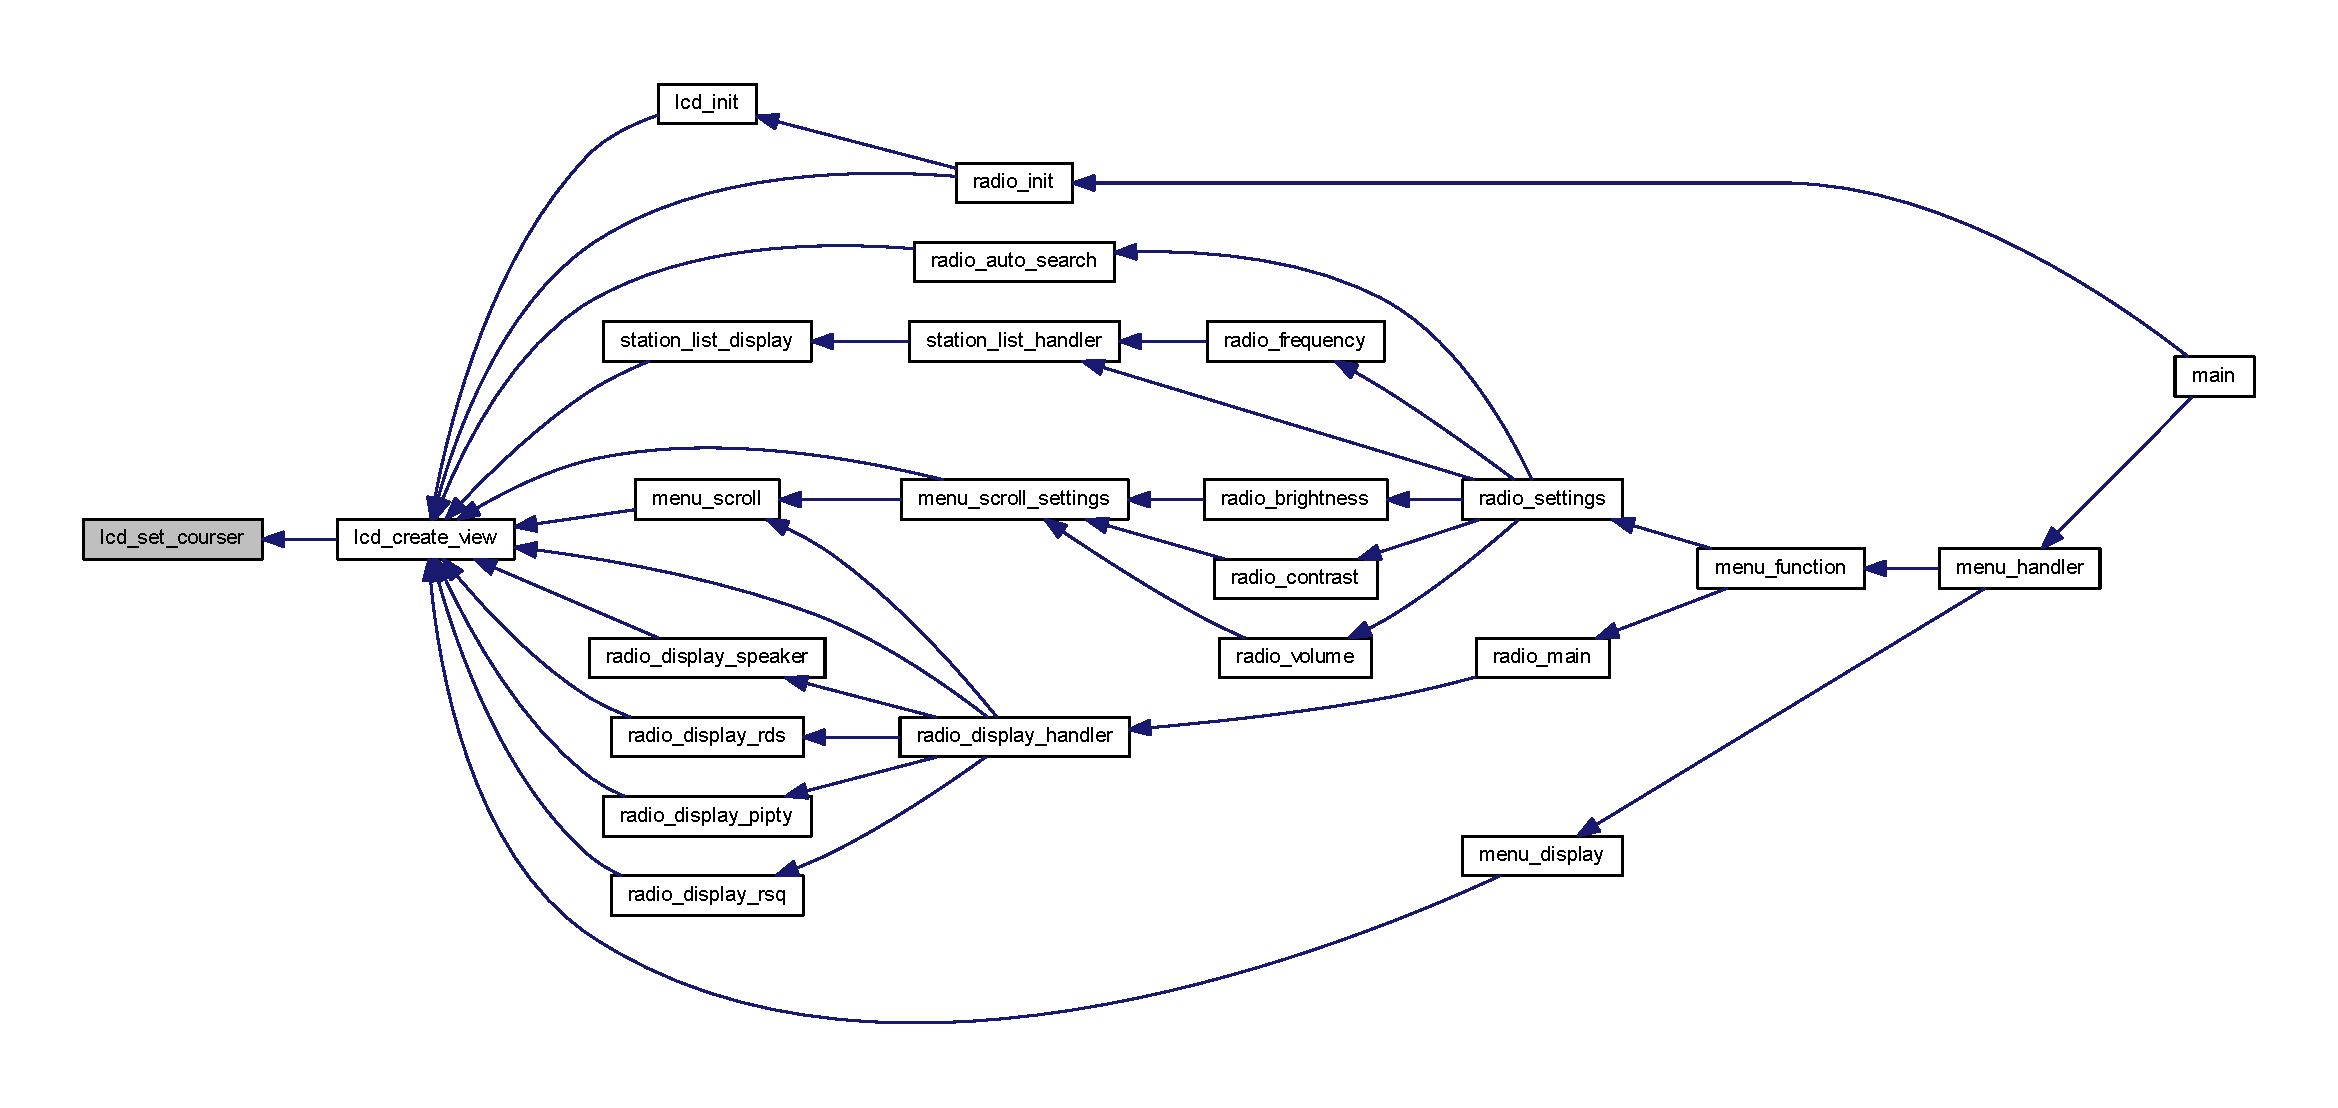
\includegraphics[width=350pt]{lcd_8h_a2a4df97ebc5b396233aa31765228ef42_icgraph}
\end{center}
\end{figure}


\hypertarget{lcd_8h_a011d26f08674b8430d53ea5e8cebd9e3}{}\index{lcd.\+h@{lcd.\+h}!lcd\+\_\+write\+\_\+char@{lcd\+\_\+write\+\_\+char}}
\index{lcd\+\_\+write\+\_\+char@{lcd\+\_\+write\+\_\+char}!lcd.\+h@{lcd.\+h}}
\subsubsection[{lcd\+\_\+write\+\_\+char}]{\setlength{\rightskip}{0pt plus 5cm}uint8\+\_\+t lcd\+\_\+write\+\_\+char (
\begin{DoxyParamCaption}
\item[{uint8\+\_\+t}]{chr}
\end{DoxyParamCaption}
)}\label{lcd_8h_a011d26f08674b8430d53ea5e8cebd9e3}


Definiert in Zeile 76 der Datei lcd.\+c.


\begin{DoxyCode}
77 \{
78 
79     \textcolor{comment}{//symbol = lcd\_replace\_special\_letter(symbol);}
80 
81     \textcolor{comment}{/*i2c\_write\_var(PCA9534\_I2C\_ADR, STOP, 1, (((symbol>>4) & 0x0f) | 0x40));}
82 \textcolor{comment}{    i2c\_write\_var(PCA9534\_I2C\_ADR, STOP, 1, (((symbol>>4) & 0x0f) | 0x50));}
83 \textcolor{comment}{    i2c\_write\_var(PCA9534\_I2C\_ADR, STOP, 1, ((symbol & 0x0f) | 0x40));}
84 \textcolor{comment}{    i2c\_write\_var(PCA9534\_I2C\_ADR, STOP, 1, ((symbol & 0x0f) | 0x50));}
85 \textcolor{comment}{    i2c\_write\_var(PCA9534\_I2C\_ADR, STOP, 1, 0x08);*/}
86 
87     \hyperlink{timer_8c_a3c56af3315c2461dec5ced585a5f84db}{\_delay\_ten\_us}(20);
88 
89     \hyperlink{i2c_8h_a6691e5911f539e1e8178c6e983e8079a}{i2c\_write\_var}(\hyperlink{pca9534_8h_a327d2e2bdf4be4cf7155f21f093b9aae}{PCA9534\_I2C\_ADR}, \hyperlink{i2c_8h_aaaea3962492fd5ad1e43cba027d949d5a679ee5320d66c8322e310daeb2ee99b8}{STOP}, 5,
90             0x00,
91             \hyperlink{lcd__commands_8h_afd4bb10e8cc3368a80abe3ef75d92c39}{LCD\_HIGHER\_BYTE}(symbol) | \hyperlink{lcd_8h_a0092100866584e3511716fbf8e39c11f}{LCD\_ENABLE\_HIGH} | 
      \hyperlink{lcd_8h_a25e9d818788f36ed74d7c4579f87f2a6}{LCD\_DATA},
92             \hyperlink{lcd__commands_8h_afd4bb10e8cc3368a80abe3ef75d92c39}{LCD\_HIGHER\_BYTE}(symbol) | \hyperlink{lcd_8h_a0cbc0c73a8326693dcae8ceac5c7b71b}{LCD\_ENABLE\_LOW}  | 
      \hyperlink{lcd_8h_a25e9d818788f36ed74d7c4579f87f2a6}{LCD\_DATA},
93             \hyperlink{lcd__commands_8h_afb9a52fe082bc759811cbc78af93e5be}{LCD\_LOWER\_BYTE}(symbol)  | \hyperlink{lcd_8h_a0092100866584e3511716fbf8e39c11f}{LCD\_ENABLE\_HIGH} | 
      \hyperlink{lcd_8h_a25e9d818788f36ed74d7c4579f87f2a6}{LCD\_DATA},
94             \hyperlink{lcd__commands_8h_afb9a52fe082bc759811cbc78af93e5be}{LCD\_LOWER\_BYTE}(symbol)  | \hyperlink{lcd_8h_a0cbc0c73a8326693dcae8ceac5c7b71b}{LCD\_ENABLE\_LOW}  | 
      \hyperlink{lcd_8h_a25e9d818788f36ed74d7c4579f87f2a6}{LCD\_DATA});
95 
96     \textcolor{keywordflow}{return} 0;
97 \}
\end{DoxyCode}


Hier ist ein Graph, der zeigt, was diese Funktion aufruft\+:\nopagebreak
\begin{figure}[H]
\begin{center}
\leavevmode
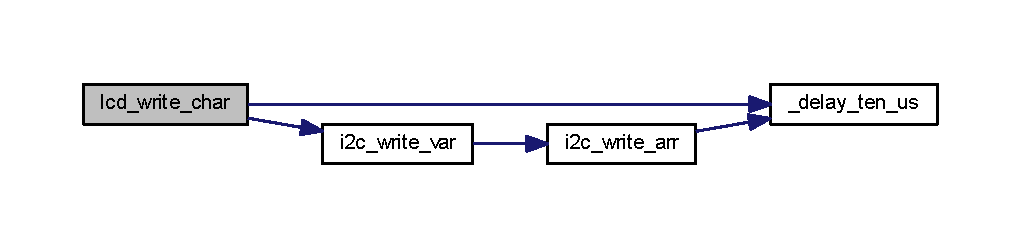
\includegraphics[width=350pt]{lcd_8h_a011d26f08674b8430d53ea5e8cebd9e3_cgraph}
\end{center}
\end{figure}




Hier ist ein Graph der zeigt, wo diese Funktion aufgerufen wird\+:\nopagebreak
\begin{figure}[H]
\begin{center}
\leavevmode
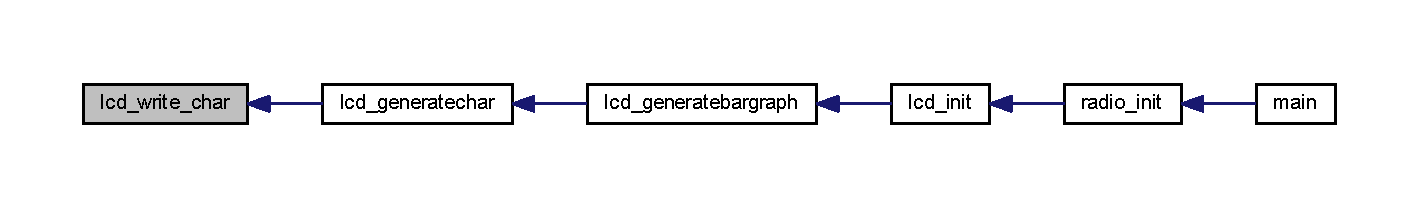
\includegraphics[width=350pt]{lcd_8h_a011d26f08674b8430d53ea5e8cebd9e3_icgraph}
\end{center}
\end{figure}


\hypertarget{lcd_8h_a2e011676f64d2ee1c854b912133ae3f9}{}\index{lcd.\+h@{lcd.\+h}!lcd\+\_\+write\+\_\+string@{lcd\+\_\+write\+\_\+string}}
\index{lcd\+\_\+write\+\_\+string@{lcd\+\_\+write\+\_\+string}!lcd.\+h@{lcd.\+h}}
\subsubsection[{lcd\+\_\+write\+\_\+string}]{\setlength{\rightskip}{0pt plus 5cm}uint8\+\_\+t lcd\+\_\+write\+\_\+string (
\begin{DoxyParamCaption}
\item[{const int8\+\_\+t $\ast$}]{str, }
\item[{uint8\+\_\+t}]{n\+\_\+bytes}
\end{DoxyParamCaption}
)}\label{lcd_8h_a2e011676f64d2ee1c854b912133ae3f9}

\hypertarget{opt3001_8h}{}\section{D\+:/\+G\+I\+T/fhradiov2/driver/opt3001.h-\/\+Dateireferenz}
\label{opt3001_8h}\index{D\+:/\+G\+I\+T/fhradiov2/driver/opt3001.\+h@{D\+:/\+G\+I\+T/fhradiov2/driver/opt3001.\+h}}
{\ttfamily \#include $<$stdint.\+h$>$}\\*
{\ttfamily \#include $<$driver/i2c.\+h$>$}\\*
Include-\/\+Abhängigkeitsdiagramm für opt3001.\+h\+:
\nopagebreak
\begin{figure}[H]
\begin{center}
\leavevmode
\includegraphics[width=350pt]{opt3001_8h__incl}
\end{center}
\end{figure}
Dieser Graph zeigt, welche Datei direkt oder indirekt diese Datei enthält\+:
\nopagebreak
\begin{figure}[H]
\begin{center}
\leavevmode
\includegraphics[width=350pt]{opt3001_8h__dep__incl}
\end{center}
\end{figure}
\subsection*{Datenstrukturen}
\begin{DoxyCompactItemize}
\item 
struct \hyperlink{structopt3001__stc}{opt3001\+\_\+stc}
\end{DoxyCompactItemize}
\subsection*{Makrodefinitionen}
\begin{DoxyCompactItemize}
\item 
\#define \hyperlink{opt3001_8h_a83c0046a2cb83309917ed6ec6b3e5b2b}{O\+P\+T3001\+\_\+\+G\+N\+D\+\_\+\+P\+I\+N}~0x00
\item 
\#define \hyperlink{opt3001_8h_a062f509618661c8536b62d247856583e}{O\+P\+T3001\+\_\+\+V\+D\+D\+\_\+\+P\+I\+N}~0x01
\item 
\#define \hyperlink{opt3001_8h_a57a9cfe5fcae1cdb426399f4f3ac8fb4}{O\+P\+T3001\+\_\+\+S\+D\+A\+\_\+\+P\+I\+N}~0x02
\item 
\#define \hyperlink{opt3001_8h_a8fa51a470988bda646bf67de9f6a8e6e}{O\+P\+T3001\+\_\+\+S\+C\+L\+\_\+\+P\+I\+N}~0x03
\item 
\#define \hyperlink{opt3001_8h_a353b66bab3e673b2969dc30b9de284d7}{O\+P\+T3001\+\_\+\+B\+A\+S\+E\+\_\+\+A\+D\+R}~0x44
\item 
\#define \hyperlink{opt3001_8h_a9af39dbc20acc60812374ca8a61899c5}{O\+P\+T3001\+\_\+\+A\+D\+R\+\_\+\+P\+I\+N}~\hyperlink{opt3001_8h_a83c0046a2cb83309917ed6ec6b3e5b2b}{O\+P\+T3001\+\_\+\+G\+N\+D\+\_\+\+P\+I\+N}
\item 
\#define \hyperlink{opt3001_8h_ad39c35e048af0890a99974e93c93cee9}{O\+P\+T3001\+\_\+\+I2\+C\+\_\+\+A\+D\+R}~(\hyperlink{opt3001_8h_a353b66bab3e673b2969dc30b9de284d7}{O\+P\+T3001\+\_\+\+B\+A\+S\+E\+\_\+\+A\+D\+R} $\vert$ \hyperlink{opt3001_8h_a9af39dbc20acc60812374ca8a61899c5}{O\+P\+T3001\+\_\+\+A\+D\+R\+\_\+\+P\+I\+N})
\item 
\#define \hyperlink{opt3001_8h_adc31d7638b454133413e5bdded688dcd}{O\+P\+T3001\+\_\+\+R\+E\+S\+U\+L\+T\+\_\+\+R\+E\+G}~0x00
\item 
\#define \hyperlink{opt3001_8h_a97a74783c7f6707babcc81aedb4cf9bc}{O\+P\+T3001\+\_\+\+C\+O\+N\+F\+I\+G\+\_\+\+R\+E\+G}~0x01
\item 
\#define \hyperlink{opt3001_8h_aa13506d6c56601c3cd1686bd4a9b757f}{O\+P\+T3001\+\_\+\+L\+\_\+\+L\+I\+M\+I\+T\+\_\+\+R\+E\+G}~0x02
\item 
\#define \hyperlink{opt3001_8h_aca3ce0064552360839f2890488ac2e6e}{O\+P\+T3001\+\_\+\+H\+\_\+\+L\+I\+M\+I\+T\+\_\+\+R\+E\+G}~0x03
\item 
\#define \hyperlink{opt3001_8h_a806311af2bb5783978e8c67f5a49ec3e}{O\+P\+T3001\+\_\+\+M\+A\+N\+U\+\_\+\+I\+D\+\_\+\+R\+E\+G}~0x7\+E
\item 
\#define \hyperlink{opt3001_8h_ab6d903ff1a1f0028b4b31aa2dc7f61ae}{O\+P\+T3001\+\_\+\+D\+E\+V\+\_\+\+I\+D\+\_\+\+R\+E\+G}~0x7\+F
\item 
\#define \hyperlink{opt3001_8h_a888795c8dd85321e189306fbc88b4510}{float\+\_\+to\+\_\+int}(value)~((value \& 0x0\+F\+F\+F\+F) $<$$<$ ((value \& 0x\+F000) $>$$>$ 12))
\end{DoxyCompactItemize}
\subsection*{Typdefinitionen}
\begin{DoxyCompactItemize}
\item 
typedef struct \hyperlink{structopt3001__stc}{opt3001\+\_\+stc} \hyperlink{opt3001_8h_a85ef6b0023cd0d3f58e5f229b4d568ed}{O\+P\+T3001\+\_\+\+S\+T\+C}
\end{DoxyCompactItemize}
\subsection*{Funktionen}
\begin{DoxyCompactItemize}
\item 
uint8\+\_\+t \hyperlink{opt3001_8h_a4910f99caac4b6293a33627107cb7e82}{opt3001\+\_\+get\+\_\+value} (uint32\+\_\+t $\ast$data)
\item 
uint8\+\_\+t \hyperlink{opt3001_8h_adc4f87c7b66e9137a35d55e0dc405bf9}{opt3001\+\_\+init} (\hyperlink{opt3001_8h_a85ef6b0023cd0d3f58e5f229b4d568ed}{O\+P\+T3001\+\_\+\+S\+T\+C} $\ast$config)
\end{DoxyCompactItemize}


\subsection{Makro-\/\+Dokumentation}
\hypertarget{opt3001_8h_a888795c8dd85321e189306fbc88b4510}{}\index{opt3001.\+h@{opt3001.\+h}!float\+\_\+to\+\_\+int@{float\+\_\+to\+\_\+int}}
\index{float\+\_\+to\+\_\+int@{float\+\_\+to\+\_\+int}!opt3001.\+h@{opt3001.\+h}}
\subsubsection[{float\+\_\+to\+\_\+int}]{\setlength{\rightskip}{0pt plus 5cm}\#define float\+\_\+to\+\_\+int(
\begin{DoxyParamCaption}
\item[{}]{value}
\end{DoxyParamCaption}
)~((value \& 0x0\+F\+F\+F\+F) $<$$<$ ((value \& 0x\+F000) $>$$>$ 12))}\label{opt3001_8h_a888795c8dd85321e189306fbc88b4510}


Definiert in Zeile 38 der Datei opt3001.\+h.

\hypertarget{opt3001_8h_a9af39dbc20acc60812374ca8a61899c5}{}\index{opt3001.\+h@{opt3001.\+h}!O\+P\+T3001\+\_\+\+A\+D\+R\+\_\+\+P\+I\+N@{O\+P\+T3001\+\_\+\+A\+D\+R\+\_\+\+P\+I\+N}}
\index{O\+P\+T3001\+\_\+\+A\+D\+R\+\_\+\+P\+I\+N@{O\+P\+T3001\+\_\+\+A\+D\+R\+\_\+\+P\+I\+N}!opt3001.\+h@{opt3001.\+h}}
\subsubsection[{O\+P\+T3001\+\_\+\+A\+D\+R\+\_\+\+P\+I\+N}]{\setlength{\rightskip}{0pt plus 5cm}\#define O\+P\+T3001\+\_\+\+A\+D\+R\+\_\+\+P\+I\+N~{\bf O\+P\+T3001\+\_\+\+G\+N\+D\+\_\+\+P\+I\+N}}\label{opt3001_8h_a9af39dbc20acc60812374ca8a61899c5}


Definiert in Zeile 19 der Datei opt3001.\+h.

\hypertarget{opt3001_8h_a353b66bab3e673b2969dc30b9de284d7}{}\index{opt3001.\+h@{opt3001.\+h}!O\+P\+T3001\+\_\+\+B\+A\+S\+E\+\_\+\+A\+D\+R@{O\+P\+T3001\+\_\+\+B\+A\+S\+E\+\_\+\+A\+D\+R}}
\index{O\+P\+T3001\+\_\+\+B\+A\+S\+E\+\_\+\+A\+D\+R@{O\+P\+T3001\+\_\+\+B\+A\+S\+E\+\_\+\+A\+D\+R}!opt3001.\+h@{opt3001.\+h}}
\subsubsection[{O\+P\+T3001\+\_\+\+B\+A\+S\+E\+\_\+\+A\+D\+R}]{\setlength{\rightskip}{0pt plus 5cm}\#define O\+P\+T3001\+\_\+\+B\+A\+S\+E\+\_\+\+A\+D\+R~0x44}\label{opt3001_8h_a353b66bab3e673b2969dc30b9de284d7}


Definiert in Zeile 18 der Datei opt3001.\+h.

\hypertarget{opt3001_8h_a97a74783c7f6707babcc81aedb4cf9bc}{}\index{opt3001.\+h@{opt3001.\+h}!O\+P\+T3001\+\_\+\+C\+O\+N\+F\+I\+G\+\_\+\+R\+E\+G@{O\+P\+T3001\+\_\+\+C\+O\+N\+F\+I\+G\+\_\+\+R\+E\+G}}
\index{O\+P\+T3001\+\_\+\+C\+O\+N\+F\+I\+G\+\_\+\+R\+E\+G@{O\+P\+T3001\+\_\+\+C\+O\+N\+F\+I\+G\+\_\+\+R\+E\+G}!opt3001.\+h@{opt3001.\+h}}
\subsubsection[{O\+P\+T3001\+\_\+\+C\+O\+N\+F\+I\+G\+\_\+\+R\+E\+G}]{\setlength{\rightskip}{0pt plus 5cm}\#define O\+P\+T3001\+\_\+\+C\+O\+N\+F\+I\+G\+\_\+\+R\+E\+G~0x01}\label{opt3001_8h_a97a74783c7f6707babcc81aedb4cf9bc}


Definiert in Zeile 23 der Datei opt3001.\+h.

\hypertarget{opt3001_8h_ab6d903ff1a1f0028b4b31aa2dc7f61ae}{}\index{opt3001.\+h@{opt3001.\+h}!O\+P\+T3001\+\_\+\+D\+E\+V\+\_\+\+I\+D\+\_\+\+R\+E\+G@{O\+P\+T3001\+\_\+\+D\+E\+V\+\_\+\+I\+D\+\_\+\+R\+E\+G}}
\index{O\+P\+T3001\+\_\+\+D\+E\+V\+\_\+\+I\+D\+\_\+\+R\+E\+G@{O\+P\+T3001\+\_\+\+D\+E\+V\+\_\+\+I\+D\+\_\+\+R\+E\+G}!opt3001.\+h@{opt3001.\+h}}
\subsubsection[{O\+P\+T3001\+\_\+\+D\+E\+V\+\_\+\+I\+D\+\_\+\+R\+E\+G}]{\setlength{\rightskip}{0pt plus 5cm}\#define O\+P\+T3001\+\_\+\+D\+E\+V\+\_\+\+I\+D\+\_\+\+R\+E\+G~0x7\+F}\label{opt3001_8h_ab6d903ff1a1f0028b4b31aa2dc7f61ae}


Definiert in Zeile 27 der Datei opt3001.\+h.

\hypertarget{opt3001_8h_a83c0046a2cb83309917ed6ec6b3e5b2b}{}\index{opt3001.\+h@{opt3001.\+h}!O\+P\+T3001\+\_\+\+G\+N\+D\+\_\+\+P\+I\+N@{O\+P\+T3001\+\_\+\+G\+N\+D\+\_\+\+P\+I\+N}}
\index{O\+P\+T3001\+\_\+\+G\+N\+D\+\_\+\+P\+I\+N@{O\+P\+T3001\+\_\+\+G\+N\+D\+\_\+\+P\+I\+N}!opt3001.\+h@{opt3001.\+h}}
\subsubsection[{O\+P\+T3001\+\_\+\+G\+N\+D\+\_\+\+P\+I\+N}]{\setlength{\rightskip}{0pt plus 5cm}\#define O\+P\+T3001\+\_\+\+G\+N\+D\+\_\+\+P\+I\+N~0x00}\label{opt3001_8h_a83c0046a2cb83309917ed6ec6b3e5b2b}


Definiert in Zeile 14 der Datei opt3001.\+h.

\hypertarget{opt3001_8h_aca3ce0064552360839f2890488ac2e6e}{}\index{opt3001.\+h@{opt3001.\+h}!O\+P\+T3001\+\_\+\+H\+\_\+\+L\+I\+M\+I\+T\+\_\+\+R\+E\+G@{O\+P\+T3001\+\_\+\+H\+\_\+\+L\+I\+M\+I\+T\+\_\+\+R\+E\+G}}
\index{O\+P\+T3001\+\_\+\+H\+\_\+\+L\+I\+M\+I\+T\+\_\+\+R\+E\+G@{O\+P\+T3001\+\_\+\+H\+\_\+\+L\+I\+M\+I\+T\+\_\+\+R\+E\+G}!opt3001.\+h@{opt3001.\+h}}
\subsubsection[{O\+P\+T3001\+\_\+\+H\+\_\+\+L\+I\+M\+I\+T\+\_\+\+R\+E\+G}]{\setlength{\rightskip}{0pt plus 5cm}\#define O\+P\+T3001\+\_\+\+H\+\_\+\+L\+I\+M\+I\+T\+\_\+\+R\+E\+G~0x03}\label{opt3001_8h_aca3ce0064552360839f2890488ac2e6e}


Definiert in Zeile 25 der Datei opt3001.\+h.

\hypertarget{opt3001_8h_ad39c35e048af0890a99974e93c93cee9}{}\index{opt3001.\+h@{opt3001.\+h}!O\+P\+T3001\+\_\+\+I2\+C\+\_\+\+A\+D\+R@{O\+P\+T3001\+\_\+\+I2\+C\+\_\+\+A\+D\+R}}
\index{O\+P\+T3001\+\_\+\+I2\+C\+\_\+\+A\+D\+R@{O\+P\+T3001\+\_\+\+I2\+C\+\_\+\+A\+D\+R}!opt3001.\+h@{opt3001.\+h}}
\subsubsection[{O\+P\+T3001\+\_\+\+I2\+C\+\_\+\+A\+D\+R}]{\setlength{\rightskip}{0pt plus 5cm}\#define O\+P\+T3001\+\_\+\+I2\+C\+\_\+\+A\+D\+R~({\bf O\+P\+T3001\+\_\+\+B\+A\+S\+E\+\_\+\+A\+D\+R} $\vert$ {\bf O\+P\+T3001\+\_\+\+A\+D\+R\+\_\+\+P\+I\+N})}\label{opt3001_8h_ad39c35e048af0890a99974e93c93cee9}


Definiert in Zeile 20 der Datei opt3001.\+h.

\hypertarget{opt3001_8h_aa13506d6c56601c3cd1686bd4a9b757f}{}\index{opt3001.\+h@{opt3001.\+h}!O\+P\+T3001\+\_\+\+L\+\_\+\+L\+I\+M\+I\+T\+\_\+\+R\+E\+G@{O\+P\+T3001\+\_\+\+L\+\_\+\+L\+I\+M\+I\+T\+\_\+\+R\+E\+G}}
\index{O\+P\+T3001\+\_\+\+L\+\_\+\+L\+I\+M\+I\+T\+\_\+\+R\+E\+G@{O\+P\+T3001\+\_\+\+L\+\_\+\+L\+I\+M\+I\+T\+\_\+\+R\+E\+G}!opt3001.\+h@{opt3001.\+h}}
\subsubsection[{O\+P\+T3001\+\_\+\+L\+\_\+\+L\+I\+M\+I\+T\+\_\+\+R\+E\+G}]{\setlength{\rightskip}{0pt plus 5cm}\#define O\+P\+T3001\+\_\+\+L\+\_\+\+L\+I\+M\+I\+T\+\_\+\+R\+E\+G~0x02}\label{opt3001_8h_aa13506d6c56601c3cd1686bd4a9b757f}


Definiert in Zeile 24 der Datei opt3001.\+h.

\hypertarget{opt3001_8h_a806311af2bb5783978e8c67f5a49ec3e}{}\index{opt3001.\+h@{opt3001.\+h}!O\+P\+T3001\+\_\+\+M\+A\+N\+U\+\_\+\+I\+D\+\_\+\+R\+E\+G@{O\+P\+T3001\+\_\+\+M\+A\+N\+U\+\_\+\+I\+D\+\_\+\+R\+E\+G}}
\index{O\+P\+T3001\+\_\+\+M\+A\+N\+U\+\_\+\+I\+D\+\_\+\+R\+E\+G@{O\+P\+T3001\+\_\+\+M\+A\+N\+U\+\_\+\+I\+D\+\_\+\+R\+E\+G}!opt3001.\+h@{opt3001.\+h}}
\subsubsection[{O\+P\+T3001\+\_\+\+M\+A\+N\+U\+\_\+\+I\+D\+\_\+\+R\+E\+G}]{\setlength{\rightskip}{0pt plus 5cm}\#define O\+P\+T3001\+\_\+\+M\+A\+N\+U\+\_\+\+I\+D\+\_\+\+R\+E\+G~0x7\+E}\label{opt3001_8h_a806311af2bb5783978e8c67f5a49ec3e}


Definiert in Zeile 26 der Datei opt3001.\+h.

\hypertarget{opt3001_8h_adc31d7638b454133413e5bdded688dcd}{}\index{opt3001.\+h@{opt3001.\+h}!O\+P\+T3001\+\_\+\+R\+E\+S\+U\+L\+T\+\_\+\+R\+E\+G@{O\+P\+T3001\+\_\+\+R\+E\+S\+U\+L\+T\+\_\+\+R\+E\+G}}
\index{O\+P\+T3001\+\_\+\+R\+E\+S\+U\+L\+T\+\_\+\+R\+E\+G@{O\+P\+T3001\+\_\+\+R\+E\+S\+U\+L\+T\+\_\+\+R\+E\+G}!opt3001.\+h@{opt3001.\+h}}
\subsubsection[{O\+P\+T3001\+\_\+\+R\+E\+S\+U\+L\+T\+\_\+\+R\+E\+G}]{\setlength{\rightskip}{0pt plus 5cm}\#define O\+P\+T3001\+\_\+\+R\+E\+S\+U\+L\+T\+\_\+\+R\+E\+G~0x00}\label{opt3001_8h_adc31d7638b454133413e5bdded688dcd}


Definiert in Zeile 22 der Datei opt3001.\+h.

\hypertarget{opt3001_8h_a8fa51a470988bda646bf67de9f6a8e6e}{}\index{opt3001.\+h@{opt3001.\+h}!O\+P\+T3001\+\_\+\+S\+C\+L\+\_\+\+P\+I\+N@{O\+P\+T3001\+\_\+\+S\+C\+L\+\_\+\+P\+I\+N}}
\index{O\+P\+T3001\+\_\+\+S\+C\+L\+\_\+\+P\+I\+N@{O\+P\+T3001\+\_\+\+S\+C\+L\+\_\+\+P\+I\+N}!opt3001.\+h@{opt3001.\+h}}
\subsubsection[{O\+P\+T3001\+\_\+\+S\+C\+L\+\_\+\+P\+I\+N}]{\setlength{\rightskip}{0pt plus 5cm}\#define O\+P\+T3001\+\_\+\+S\+C\+L\+\_\+\+P\+I\+N~0x03}\label{opt3001_8h_a8fa51a470988bda646bf67de9f6a8e6e}


Definiert in Zeile 17 der Datei opt3001.\+h.

\hypertarget{opt3001_8h_a57a9cfe5fcae1cdb426399f4f3ac8fb4}{}\index{opt3001.\+h@{opt3001.\+h}!O\+P\+T3001\+\_\+\+S\+D\+A\+\_\+\+P\+I\+N@{O\+P\+T3001\+\_\+\+S\+D\+A\+\_\+\+P\+I\+N}}
\index{O\+P\+T3001\+\_\+\+S\+D\+A\+\_\+\+P\+I\+N@{O\+P\+T3001\+\_\+\+S\+D\+A\+\_\+\+P\+I\+N}!opt3001.\+h@{opt3001.\+h}}
\subsubsection[{O\+P\+T3001\+\_\+\+S\+D\+A\+\_\+\+P\+I\+N}]{\setlength{\rightskip}{0pt plus 5cm}\#define O\+P\+T3001\+\_\+\+S\+D\+A\+\_\+\+P\+I\+N~0x02}\label{opt3001_8h_a57a9cfe5fcae1cdb426399f4f3ac8fb4}


Definiert in Zeile 16 der Datei opt3001.\+h.

\hypertarget{opt3001_8h_a062f509618661c8536b62d247856583e}{}\index{opt3001.\+h@{opt3001.\+h}!O\+P\+T3001\+\_\+\+V\+D\+D\+\_\+\+P\+I\+N@{O\+P\+T3001\+\_\+\+V\+D\+D\+\_\+\+P\+I\+N}}
\index{O\+P\+T3001\+\_\+\+V\+D\+D\+\_\+\+P\+I\+N@{O\+P\+T3001\+\_\+\+V\+D\+D\+\_\+\+P\+I\+N}!opt3001.\+h@{opt3001.\+h}}
\subsubsection[{O\+P\+T3001\+\_\+\+V\+D\+D\+\_\+\+P\+I\+N}]{\setlength{\rightskip}{0pt plus 5cm}\#define O\+P\+T3001\+\_\+\+V\+D\+D\+\_\+\+P\+I\+N~0x01}\label{opt3001_8h_a062f509618661c8536b62d247856583e}


Definiert in Zeile 15 der Datei opt3001.\+h.



\subsection{Dokumentation der benutzerdefinierten Typen}
\hypertarget{opt3001_8h_a85ef6b0023cd0d3f58e5f229b4d568ed}{}\index{opt3001.\+h@{opt3001.\+h}!O\+P\+T3001\+\_\+\+S\+T\+C@{O\+P\+T3001\+\_\+\+S\+T\+C}}
\index{O\+P\+T3001\+\_\+\+S\+T\+C@{O\+P\+T3001\+\_\+\+S\+T\+C}!opt3001.\+h@{opt3001.\+h}}
\subsubsection[{O\+P\+T3001\+\_\+\+S\+T\+C}]{\setlength{\rightskip}{0pt plus 5cm}typedef struct {\bf opt3001\+\_\+stc}  {\bf O\+P\+T3001\+\_\+\+S\+T\+C}}\label{opt3001_8h_a85ef6b0023cd0d3f58e5f229b4d568ed}


\subsection{Dokumentation der Funktionen}
\hypertarget{opt3001_8h_a4910f99caac4b6293a33627107cb7e82}{}\index{opt3001.\+h@{opt3001.\+h}!opt3001\+\_\+get\+\_\+value@{opt3001\+\_\+get\+\_\+value}}
\index{opt3001\+\_\+get\+\_\+value@{opt3001\+\_\+get\+\_\+value}!opt3001.\+h@{opt3001.\+h}}
\subsubsection[{opt3001\+\_\+get\+\_\+value}]{\setlength{\rightskip}{0pt plus 5cm}uint8\+\_\+t opt3001\+\_\+get\+\_\+value (
\begin{DoxyParamCaption}
\item[{uint32\+\_\+t $\ast$}]{data}
\end{DoxyParamCaption}
)}\label{opt3001_8h_a4910f99caac4b6293a33627107cb7e82}


Definiert in Zeile 19 der Datei opt3001.\+c.


\begin{DoxyCode}
20 \{
21     \textcolor{keyword}{union }\{
22         uint8\_t bytes[2];
23         uint16\_t byte;
24     \}value;
25 
26     uint8\_t resp[2];
27 
28     \hyperlink{i2c_8h_a6691e5911f539e1e8178c6e983e8079a}{i2c\_write\_var}(\hyperlink{opt3001_8h_ad39c35e048af0890a99974e93c93cee9}{OPT3001\_I2C\_ADR}, \hyperlink{i2c_8h_aaaea3962492fd5ad1e43cba027d949d5a807d17ddb75240ddeede2c54fd79bd40}{REPT}, 1, 
      \hyperlink{opt3001_8h_adc31d7638b454133413e5bdded688dcd}{OPT3001\_RESULT\_REG});
29     \hyperlink{i2c_8h_a6dd896b0c82d1aa91a1a8155b41c4566}{i2c\_read}(\hyperlink{opt3001_8h_ad39c35e048af0890a99974e93c93cee9}{OPT3001\_I2C\_ADR}, \hyperlink{i2c_8h_aaaea3962492fd5ad1e43cba027d949d5a679ee5320d66c8322e310daeb2ee99b8}{STOP}, 2, resp);
30 
31     value.bytes[0] = resp[1];
32     value.bytes[1] = resp[0];
33     \textcolor{comment}{/* Get actual value over I2C and combine higher byte and lower byte */}
34     *data = ((value.byte & 0x0FFFF) << ((value.byte & 0xF000) >> 12));
35     \textcolor{keywordflow}{return} 0;
36 \}
\end{DoxyCode}


Hier ist ein Graph, der zeigt, was diese Funktion aufruft\+:\nopagebreak
\begin{figure}[H]
\begin{center}
\leavevmode
\includegraphics[width=350pt]{opt3001_8h_a4910f99caac4b6293a33627107cb7e82_cgraph}
\end{center}
\end{figure}




Hier ist ein Graph der zeigt, wo diese Funktion aufgerufen wird\+:\nopagebreak
\begin{figure}[H]
\begin{center}
\leavevmode
\includegraphics[width=325pt]{opt3001_8h_a4910f99caac4b6293a33627107cb7e82_icgraph}
\end{center}
\end{figure}


\hypertarget{opt3001_8h_adc4f87c7b66e9137a35d55e0dc405bf9}{}\index{opt3001.\+h@{opt3001.\+h}!opt3001\+\_\+init@{opt3001\+\_\+init}}
\index{opt3001\+\_\+init@{opt3001\+\_\+init}!opt3001.\+h@{opt3001.\+h}}
\subsubsection[{opt3001\+\_\+init}]{\setlength{\rightskip}{0pt plus 5cm}uint8\+\_\+t opt3001\+\_\+init (
\begin{DoxyParamCaption}
\item[{{\bf O\+P\+T3001\+\_\+\+S\+T\+C} $\ast$}]{config}
\end{DoxyParamCaption}
)}\label{opt3001_8h_adc4f87c7b66e9137a35d55e0dc405bf9}


Definiert in Zeile 10 der Datei opt3001.\+c.


\begin{DoxyCode}
11 \{
12     \hyperlink{i2c_8h_a6691e5911f539e1e8178c6e983e8079a}{i2c\_write\_var}(\hyperlink{opt3001_8h_ad39c35e048af0890a99974e93c93cee9}{OPT3001\_I2C\_ADR}, \hyperlink{i2c_8h_aaaea3962492fd5ad1e43cba027d949d5a679ee5320d66c8322e310daeb2ee99b8}{STOP}, 3, 
      \hyperlink{opt3001_8h_a97a74783c7f6707babcc81aedb4cf9bc}{OPT3001\_CONFIG\_REG}, config->\hyperlink{structopt3001__stc_aa26297bc57b4b74262246d02175f4308}{config}); \textcolor{comment}{//TODO split in high and low byte}
13     \hyperlink{i2c_8h_a6691e5911f539e1e8178c6e983e8079a}{i2c\_write\_var}(\hyperlink{opt3001_8h_ad39c35e048af0890a99974e93c93cee9}{OPT3001\_I2C\_ADR}, \hyperlink{i2c_8h_aaaea3962492fd5ad1e43cba027d949d5a679ee5320d66c8322e310daeb2ee99b8}{STOP}, 3, 
      \hyperlink{opt3001_8h_aa13506d6c56601c3cd1686bd4a9b757f}{OPT3001\_L\_LIMIT\_REG}, config->\hyperlink{structopt3001__stc_a5561e4eedc9af4ceb86ed5056241bf77}{low\_limit}); \textcolor{comment}{//TODO split in high and low byte}
14     \hyperlink{i2c_8h_a6691e5911f539e1e8178c6e983e8079a}{i2c\_write\_var}(\hyperlink{opt3001_8h_ad39c35e048af0890a99974e93c93cee9}{OPT3001\_I2C\_ADR}, \hyperlink{i2c_8h_aaaea3962492fd5ad1e43cba027d949d5a679ee5320d66c8322e310daeb2ee99b8}{STOP}, 3, 
      \hyperlink{opt3001_8h_aca3ce0064552360839f2890488ac2e6e}{OPT3001\_H\_LIMIT\_REG}, config->\hyperlink{structopt3001__stc_af121d4246e275920873b33ad155fa9ba}{high\_limit}); \textcolor{comment}{//TODO split in high and low byte}
15     \textcolor{comment}{/* Some I2C writes for first configuration on OPT3001 */}
16     \textcolor{keywordflow}{return} 0;
17 \}
\end{DoxyCode}


Hier ist ein Graph, der zeigt, was diese Funktion aufruft\+:\nopagebreak
\begin{figure}[H]
\begin{center}
\leavevmode
\includegraphics[width=350pt]{opt3001_8h_adc4f87c7b66e9137a35d55e0dc405bf9_cgraph}
\end{center}
\end{figure}



\hypertarget{pca9530_8h}{}\section{driver/pca9530.h-\/\+Dateireferenz}
\label{pca9530_8h}\index{driver/pca9530.\+h@{driver/pca9530.\+h}}
{\ttfamily \#include $<$stdint.\+h$>$}\\*
{\ttfamily \#include $<$driver/i2c.\+h$>$}\\*
Include-\/\+Abhängigkeitsdiagramm für pca9530.\+h\+:\nopagebreak
\begin{figure}[H]
\begin{center}
\leavevmode
\includegraphics[width=350pt]{pca9530_8h__incl}
\end{center}
\end{figure}
Dieser Graph zeigt, welche Datei direkt oder indirekt diese Datei enthält\+:\nopagebreak
\begin{figure}[H]
\begin{center}
\leavevmode
\includegraphics[width=350pt]{pca9530_8h__dep__incl}
\end{center}
\end{figure}
\subsection*{Datenstrukturen}
\begin{DoxyCompactItemize}
\item 
struct \hyperlink{structpca9530__ctl}{pca9530\+\_\+ctl}
\item 
struct \hyperlink{structpca9530__in}{pca9530\+\_\+in}
\item 
struct \hyperlink{structpca9530__sel}{pca9530\+\_\+sel}
\item 
struct \hyperlink{structpca9530}{pca9530}
\end{DoxyCompactItemize}
\subsection*{Makrodefinitionen}
\begin{DoxyCompactItemize}
\item 
\#define \hyperlink{pca9530_8h_a566fb06c05caecf304dfe9a0bb657b34}{P\+C\+A9530\+\_\+\+I2\+C\+\_\+\+S\+T\+D\+\_\+\+A\+D\+R}~0x60
\item 
\#define \hyperlink{pca9530_8h_a554cc61fe4234ac4c4eafa0b4977175c}{P\+C\+A9530\+\_\+\+I2\+C\+\_\+\+A0\+\_\+\+B\+I\+T}~0
\item 
\#define \hyperlink{pca9530_8h_a9ad00301c1ffc3a81b0f912ba863238b}{P\+C\+A9530\+\_\+\+I2\+C\+\_\+\+A\+D\+R}~(\hyperlink{pca9530_8h_a566fb06c05caecf304dfe9a0bb657b34}{P\+C\+A9530\+\_\+\+I2\+C\+\_\+\+S\+T\+D\+\_\+\+A\+D\+R} $\vert$ \hyperlink{pca9530_8h_a554cc61fe4234ac4c4eafa0b4977175c}{P\+C\+A9530\+\_\+\+I2\+C\+\_\+\+A0\+\_\+\+B\+I\+T})
\end{DoxyCompactItemize}
\subsection*{Typdefinitionen}
\begin{DoxyCompactItemize}
\item 
typedef struct \hyperlink{structpca9530__ctl}{pca9530\+\_\+ctl} \hyperlink{pca9530_8h_ab385b8535f80ceababc3fd9d0f15b045}{P\+C\+A9530\+\_\+\+C\+T\+L}
\item 
typedef struct \hyperlink{structpca9530__in}{pca9530\+\_\+in} \hyperlink{pca9530_8h_a2e7c59b702993415a25765895971bc16}{P\+C\+A9530\+\_\+\+I\+N}
\item 
typedef struct \hyperlink{structpca9530__sel}{pca9530\+\_\+sel} \hyperlink{pca9530_8h_a10250afacff108ca56d8080a27aa91a0}{P\+C\+A9530\+\_\+\+S\+E\+L}
\item 
typedef struct \hyperlink{structpca9530}{pca9530} \hyperlink{pca9530_8h_a837a42b4ed8a83b5aee92843449537bf}{P\+C\+A9530}
\end{DoxyCompactItemize}
\subsection*{Aufzählungen}
\begin{DoxyCompactItemize}
\item 
enum \hyperlink{pca9530_8h_a12bddc4690ce327030f243e8d2767962}{P\+C\+A9530\+\_\+\+C\+T\+R\+L\+\_\+\+C\+M\+D} \{ \\*
\hyperlink{pca9530_8h_a12bddc4690ce327030f243e8d2767962ae310c909d76b003d016bef8bdf16936a}{I\+N\+P\+U\+T} = 0, 
\hyperlink{pca9530_8h_a12bddc4690ce327030f243e8d2767962a2f0bf80b9c8a16fc25723db25380ec45}{P\+S\+C0}, 
\hyperlink{pca9530_8h_a12bddc4690ce327030f243e8d2767962a4969f4b49dd00aa89aa0b6b3a7cce0cc}{P\+W\+M0}, 
\hyperlink{pca9530_8h_a12bddc4690ce327030f243e8d2767962a779992e73fedde2672b79061e7f785b3}{P\+S\+C1}, 
\\*
\hyperlink{pca9530_8h_a12bddc4690ce327030f243e8d2767962acc6ab0fb66c5ba52524e32ea2ad0bd1a}{P\+W\+M1}, 
\hyperlink{pca9530_8h_a12bddc4690ce327030f243e8d2767962a5feb25e13e5f0c37661a4287511b89ad}{L\+S0}
 \}
\item 
enum \hyperlink{pca9530_8h_ace2d36a1fc0cc58626736636eaff2237}{P\+C\+A9530\+\_\+\+L\+E\+D\+\_\+\+S\+T\+A\+T\+E} \{ \hyperlink{pca9530_8h_ace2d36a1fc0cc58626736636eaff2237afc0ca8cc6cbe215fd3f1ae6d40255b40}{L\+E\+D\+\_\+\+O\+F\+F} = 0, 
\hyperlink{pca9530_8h_ace2d36a1fc0cc58626736636eaff2237add01b80eb93658fb4cf7eb9aceb89a1d}{L\+E\+D\+\_\+\+O\+N}, 
\hyperlink{pca9530_8h_ace2d36a1fc0cc58626736636eaff2237ab29666bb955e9656797711ee1a2f6932}{P\+W\+M0\+\_\+\+R\+A\+T\+E}, 
\hyperlink{pca9530_8h_ace2d36a1fc0cc58626736636eaff2237a237ba94dca5793632d0e6694a68bf248}{P\+W\+M1\+\_\+\+R\+A\+T\+E}
 \}
\item 
enum \hyperlink{pca9530_8h_a8987674a0fcf29a23cf9d1d8886a3ce8}{P\+C\+A9530\+\_\+\+F\+R\+E\+Q} \{ \hyperlink{pca9530_8h_a8987674a0fcf29a23cf9d1d8886a3ce8a32ea2e2a12cd46becf9ec1e762ab17ca}{F\+R\+E\+Q\+\_\+0} = 0, 
\hyperlink{pca9530_8h_a8987674a0fcf29a23cf9d1d8886a3ce8a3f791392d54d23b2388610584b6c72d7}{F\+R\+E\+Q\+\_\+1}
 \}
\item 
enum \hyperlink{pca9530_8h_abc74a5690ccc2a8341463459d2089d9a}{P\+C\+A9530\+\_\+\+P\+W\+M} \{ \hyperlink{pca9530_8h_abc74a5690ccc2a8341463459d2089d9aa857e21e20c27df92dec4574fcddfd740}{P\+W\+M\+\_\+0} = 0, 
\hyperlink{pca9530_8h_abc74a5690ccc2a8341463459d2089d9aaea3b5b1dcb8647c430bc9391799f4703}{P\+W\+M\+\_\+1}
 \}
\end{DoxyCompactItemize}
\subsection*{Funktionen}
\begin{DoxyCompactItemize}
\item 
uint8\+\_\+t \hyperlink{pca9530_8h_abc69b1cb491825b0e425539994b188bb}{pca9530\+\_\+set\+\_\+freq} (enum \hyperlink{pca9530_8h_a8987674a0fcf29a23cf9d1d8886a3ce8}{P\+C\+A9530\+\_\+\+F\+R\+E\+Q} freq\+\_\+sel, uint8\+\_\+t freq)
\item 
uint8\+\_\+t \hyperlink{pca9530_8h_a07bd06dbfcb216eedc1969aa04e19b53}{pca9530\+\_\+set\+\_\+pwm} (enum \hyperlink{pca9530_8h_abc74a5690ccc2a8341463459d2089d9a}{P\+C\+A9530\+\_\+\+P\+W\+M} pwm\+\_\+sel, uint8\+\_\+t pwm)
\item 
uint8\+\_\+t \hyperlink{pca9530_8h_a7abe5b75b4137ce2bd840a939d8b61d1}{pca9530\+\_\+config\+\_\+led} (enum \hyperlink{pca9530_8h_ace2d36a1fc0cc58626736636eaff2237}{P\+C\+A9530\+\_\+\+L\+E\+D\+\_\+\+S\+T\+A\+T\+E} led0\+\_\+state, enum \hyperlink{pca9530_8h_ace2d36a1fc0cc58626736636eaff2237}{P\+C\+A9530\+\_\+\+L\+E\+D\+\_\+\+S\+T\+A\+T\+E} led1\+\_\+state)
\item 
uint8\+\_\+t \hyperlink{pca9530_8h_a0504ea065814c638843035fe0559b24c}{pca9530\+\_\+read\+\_\+input} ()
\item 
uint8\+\_\+t \hyperlink{pca9530_8h_ae2f44601e0bbf4c0b7bbdb127def81c3}{pca9530\+\_\+init} (const \hyperlink{pca9530_8h_a837a42b4ed8a83b5aee92843449537bf}{P\+C\+A9530} $\ast$config)
\end{DoxyCompactItemize}


\subsection{Makro-\/\+Dokumentation}
\hypertarget{pca9530_8h_a554cc61fe4234ac4c4eafa0b4977175c}{}\index{pca9530.\+h@{pca9530.\+h}!P\+C\+A9530\+\_\+\+I2\+C\+\_\+\+A0\+\_\+\+B\+I\+T@{P\+C\+A9530\+\_\+\+I2\+C\+\_\+\+A0\+\_\+\+B\+I\+T}}
\index{P\+C\+A9530\+\_\+\+I2\+C\+\_\+\+A0\+\_\+\+B\+I\+T@{P\+C\+A9530\+\_\+\+I2\+C\+\_\+\+A0\+\_\+\+B\+I\+T}!pca9530.\+h@{pca9530.\+h}}
\subsubsection[{P\+C\+A9530\+\_\+\+I2\+C\+\_\+\+A0\+\_\+\+B\+I\+T}]{\setlength{\rightskip}{0pt plus 5cm}\#define P\+C\+A9530\+\_\+\+I2\+C\+\_\+\+A0\+\_\+\+B\+I\+T~0}\label{pca9530_8h_a554cc61fe4234ac4c4eafa0b4977175c}


Definiert in Zeile 15 der Datei pca9530.\+h.

\hypertarget{pca9530_8h_a9ad00301c1ffc3a81b0f912ba863238b}{}\index{pca9530.\+h@{pca9530.\+h}!P\+C\+A9530\+\_\+\+I2\+C\+\_\+\+A\+D\+R@{P\+C\+A9530\+\_\+\+I2\+C\+\_\+\+A\+D\+R}}
\index{P\+C\+A9530\+\_\+\+I2\+C\+\_\+\+A\+D\+R@{P\+C\+A9530\+\_\+\+I2\+C\+\_\+\+A\+D\+R}!pca9530.\+h@{pca9530.\+h}}
\subsubsection[{P\+C\+A9530\+\_\+\+I2\+C\+\_\+\+A\+D\+R}]{\setlength{\rightskip}{0pt plus 5cm}\#define P\+C\+A9530\+\_\+\+I2\+C\+\_\+\+A\+D\+R~({\bf P\+C\+A9530\+\_\+\+I2\+C\+\_\+\+S\+T\+D\+\_\+\+A\+D\+R} $\vert$ {\bf P\+C\+A9530\+\_\+\+I2\+C\+\_\+\+A0\+\_\+\+B\+I\+T})}\label{pca9530_8h_a9ad00301c1ffc3a81b0f912ba863238b}


Definiert in Zeile 16 der Datei pca9530.\+h.

\hypertarget{pca9530_8h_a566fb06c05caecf304dfe9a0bb657b34}{}\index{pca9530.\+h@{pca9530.\+h}!P\+C\+A9530\+\_\+\+I2\+C\+\_\+\+S\+T\+D\+\_\+\+A\+D\+R@{P\+C\+A9530\+\_\+\+I2\+C\+\_\+\+S\+T\+D\+\_\+\+A\+D\+R}}
\index{P\+C\+A9530\+\_\+\+I2\+C\+\_\+\+S\+T\+D\+\_\+\+A\+D\+R@{P\+C\+A9530\+\_\+\+I2\+C\+\_\+\+S\+T\+D\+\_\+\+A\+D\+R}!pca9530.\+h@{pca9530.\+h}}
\subsubsection[{P\+C\+A9530\+\_\+\+I2\+C\+\_\+\+S\+T\+D\+\_\+\+A\+D\+R}]{\setlength{\rightskip}{0pt plus 5cm}\#define P\+C\+A9530\+\_\+\+I2\+C\+\_\+\+S\+T\+D\+\_\+\+A\+D\+R~0x60}\label{pca9530_8h_a566fb06c05caecf304dfe9a0bb657b34}


Definiert in Zeile 14 der Datei pca9530.\+h.



\subsection{Dokumentation der benutzerdefinierten Typen}
\hypertarget{pca9530_8h_a837a42b4ed8a83b5aee92843449537bf}{}\index{pca9530.\+h@{pca9530.\+h}!P\+C\+A9530@{P\+C\+A9530}}
\index{P\+C\+A9530@{P\+C\+A9530}!pca9530.\+h@{pca9530.\+h}}
\subsubsection[{P\+C\+A9530}]{\setlength{\rightskip}{0pt plus 5cm}typedef struct {\bf pca9530}  {\bf P\+C\+A9530}}\label{pca9530_8h_a837a42b4ed8a83b5aee92843449537bf}
\hypertarget{pca9530_8h_ab385b8535f80ceababc3fd9d0f15b045}{}\index{pca9530.\+h@{pca9530.\+h}!P\+C\+A9530\+\_\+\+C\+T\+L@{P\+C\+A9530\+\_\+\+C\+T\+L}}
\index{P\+C\+A9530\+\_\+\+C\+T\+L@{P\+C\+A9530\+\_\+\+C\+T\+L}!pca9530.\+h@{pca9530.\+h}}
\subsubsection[{P\+C\+A9530\+\_\+\+C\+T\+L}]{\setlength{\rightskip}{0pt plus 5cm}typedef struct {\bf pca9530\+\_\+ctl}  {\bf P\+C\+A9530\+\_\+\+C\+T\+L}}\label{pca9530_8h_ab385b8535f80ceababc3fd9d0f15b045}
\hypertarget{pca9530_8h_a2e7c59b702993415a25765895971bc16}{}\index{pca9530.\+h@{pca9530.\+h}!P\+C\+A9530\+\_\+\+I\+N@{P\+C\+A9530\+\_\+\+I\+N}}
\index{P\+C\+A9530\+\_\+\+I\+N@{P\+C\+A9530\+\_\+\+I\+N}!pca9530.\+h@{pca9530.\+h}}
\subsubsection[{P\+C\+A9530\+\_\+\+I\+N}]{\setlength{\rightskip}{0pt plus 5cm}typedef struct {\bf pca9530\+\_\+in}  {\bf P\+C\+A9530\+\_\+\+I\+N}}\label{pca9530_8h_a2e7c59b702993415a25765895971bc16}
\hypertarget{pca9530_8h_a10250afacff108ca56d8080a27aa91a0}{}\index{pca9530.\+h@{pca9530.\+h}!P\+C\+A9530\+\_\+\+S\+E\+L@{P\+C\+A9530\+\_\+\+S\+E\+L}}
\index{P\+C\+A9530\+\_\+\+S\+E\+L@{P\+C\+A9530\+\_\+\+S\+E\+L}!pca9530.\+h@{pca9530.\+h}}
\subsubsection[{P\+C\+A9530\+\_\+\+S\+E\+L}]{\setlength{\rightskip}{0pt plus 5cm}typedef struct {\bf pca9530\+\_\+sel}  {\bf P\+C\+A9530\+\_\+\+S\+E\+L}}\label{pca9530_8h_a10250afacff108ca56d8080a27aa91a0}


\subsection{Dokumentation der Aufzählungstypen}
\hypertarget{pca9530_8h_a12bddc4690ce327030f243e8d2767962}{}\index{pca9530.\+h@{pca9530.\+h}!P\+C\+A9530\+\_\+\+C\+T\+R\+L\+\_\+\+C\+M\+D@{P\+C\+A9530\+\_\+\+C\+T\+R\+L\+\_\+\+C\+M\+D}}
\index{P\+C\+A9530\+\_\+\+C\+T\+R\+L\+\_\+\+C\+M\+D@{P\+C\+A9530\+\_\+\+C\+T\+R\+L\+\_\+\+C\+M\+D}!pca9530.\+h@{pca9530.\+h}}
\subsubsection[{P\+C\+A9530\+\_\+\+C\+T\+R\+L\+\_\+\+C\+M\+D}]{\setlength{\rightskip}{0pt plus 5cm}enum {\bf P\+C\+A9530\+\_\+\+C\+T\+R\+L\+\_\+\+C\+M\+D}}\label{pca9530_8h_a12bddc4690ce327030f243e8d2767962}
\begin{Desc}
\item[Aufzählungswerte]\par
\begin{description}
\index{I\+N\+P\+U\+T@{I\+N\+P\+U\+T}!pca9530.\+h@{pca9530.\+h}}\index{pca9530.\+h@{pca9530.\+h}!I\+N\+P\+U\+T@{I\+N\+P\+U\+T}}\item[{\em 
\hypertarget{pca9530_8h_a12bddc4690ce327030f243e8d2767962ae310c909d76b003d016bef8bdf16936a}{}I\+N\+P\+U\+T\label{pca9530_8h_a12bddc4690ce327030f243e8d2767962ae310c909d76b003d016bef8bdf16936a}
}]\index{P\+S\+C0@{P\+S\+C0}!pca9530.\+h@{pca9530.\+h}}\index{pca9530.\+h@{pca9530.\+h}!P\+S\+C0@{P\+S\+C0}}\item[{\em 
\hypertarget{pca9530_8h_a12bddc4690ce327030f243e8d2767962a2f0bf80b9c8a16fc25723db25380ec45}{}P\+S\+C0\label{pca9530_8h_a12bddc4690ce327030f243e8d2767962a2f0bf80b9c8a16fc25723db25380ec45}
}]\index{P\+W\+M0@{P\+W\+M0}!pca9530.\+h@{pca9530.\+h}}\index{pca9530.\+h@{pca9530.\+h}!P\+W\+M0@{P\+W\+M0}}\item[{\em 
\hypertarget{pca9530_8h_a12bddc4690ce327030f243e8d2767962a4969f4b49dd00aa89aa0b6b3a7cce0cc}{}P\+W\+M0\label{pca9530_8h_a12bddc4690ce327030f243e8d2767962a4969f4b49dd00aa89aa0b6b3a7cce0cc}
}]\index{P\+S\+C1@{P\+S\+C1}!pca9530.\+h@{pca9530.\+h}}\index{pca9530.\+h@{pca9530.\+h}!P\+S\+C1@{P\+S\+C1}}\item[{\em 
\hypertarget{pca9530_8h_a12bddc4690ce327030f243e8d2767962a779992e73fedde2672b79061e7f785b3}{}P\+S\+C1\label{pca9530_8h_a12bddc4690ce327030f243e8d2767962a779992e73fedde2672b79061e7f785b3}
}]\index{P\+W\+M1@{P\+W\+M1}!pca9530.\+h@{pca9530.\+h}}\index{pca9530.\+h@{pca9530.\+h}!P\+W\+M1@{P\+W\+M1}}\item[{\em 
\hypertarget{pca9530_8h_a12bddc4690ce327030f243e8d2767962acc6ab0fb66c5ba52524e32ea2ad0bd1a}{}P\+W\+M1\label{pca9530_8h_a12bddc4690ce327030f243e8d2767962acc6ab0fb66c5ba52524e32ea2ad0bd1a}
}]\index{L\+S0@{L\+S0}!pca9530.\+h@{pca9530.\+h}}\index{pca9530.\+h@{pca9530.\+h}!L\+S0@{L\+S0}}\item[{\em 
\hypertarget{pca9530_8h_a12bddc4690ce327030f243e8d2767962a5feb25e13e5f0c37661a4287511b89ad}{}L\+S0\label{pca9530_8h_a12bddc4690ce327030f243e8d2767962a5feb25e13e5f0c37661a4287511b89ad}
}]\end{description}
\end{Desc}


Definiert in Zeile 19 der Datei pca9530.\+h.


\begin{DoxyCode}
19                       \{
20     \hyperlink{pca9530_8h_a12bddc4690ce327030f243e8d2767962ae310c909d76b003d016bef8bdf16936a}{INPUT} = 0,
21     \hyperlink{pca9530_8h_a12bddc4690ce327030f243e8d2767962a2f0bf80b9c8a16fc25723db25380ec45}{PSC0},
22     \hyperlink{pca9530_8h_a12bddc4690ce327030f243e8d2767962a4969f4b49dd00aa89aa0b6b3a7cce0cc}{PWM0},
23     \hyperlink{pca9530_8h_a12bddc4690ce327030f243e8d2767962a779992e73fedde2672b79061e7f785b3}{PSC1},
24     \hyperlink{pca9530_8h_a12bddc4690ce327030f243e8d2767962acc6ab0fb66c5ba52524e32ea2ad0bd1a}{PWM1},
25     \hyperlink{pca9530_8h_a12bddc4690ce327030f243e8d2767962a5feb25e13e5f0c37661a4287511b89ad}{LS0}
26 \};
\end{DoxyCode}
\hypertarget{pca9530_8h_a8987674a0fcf29a23cf9d1d8886a3ce8}{}\index{pca9530.\+h@{pca9530.\+h}!P\+C\+A9530\+\_\+\+F\+R\+E\+Q@{P\+C\+A9530\+\_\+\+F\+R\+E\+Q}}
\index{P\+C\+A9530\+\_\+\+F\+R\+E\+Q@{P\+C\+A9530\+\_\+\+F\+R\+E\+Q}!pca9530.\+h@{pca9530.\+h}}
\subsubsection[{P\+C\+A9530\+\_\+\+F\+R\+E\+Q}]{\setlength{\rightskip}{0pt plus 5cm}enum {\bf P\+C\+A9530\+\_\+\+F\+R\+E\+Q}}\label{pca9530_8h_a8987674a0fcf29a23cf9d1d8886a3ce8}
\begin{Desc}
\item[Aufzählungswerte]\par
\begin{description}
\index{F\+R\+E\+Q\+\_\+0@{F\+R\+E\+Q\+\_\+0}!pca9530.\+h@{pca9530.\+h}}\index{pca9530.\+h@{pca9530.\+h}!F\+R\+E\+Q\+\_\+0@{F\+R\+E\+Q\+\_\+0}}\item[{\em 
\hypertarget{pca9530_8h_a8987674a0fcf29a23cf9d1d8886a3ce8a32ea2e2a12cd46becf9ec1e762ab17ca}{}F\+R\+E\+Q\+\_\+0\label{pca9530_8h_a8987674a0fcf29a23cf9d1d8886a3ce8a32ea2e2a12cd46becf9ec1e762ab17ca}
}]\index{F\+R\+E\+Q\+\_\+1@{F\+R\+E\+Q\+\_\+1}!pca9530.\+h@{pca9530.\+h}}\index{pca9530.\+h@{pca9530.\+h}!F\+R\+E\+Q\+\_\+1@{F\+R\+E\+Q\+\_\+1}}\item[{\em 
\hypertarget{pca9530_8h_a8987674a0fcf29a23cf9d1d8886a3ce8a3f791392d54d23b2388610584b6c72d7}{}F\+R\+E\+Q\+\_\+1\label{pca9530_8h_a8987674a0fcf29a23cf9d1d8886a3ce8a3f791392d54d23b2388610584b6c72d7}
}]\end{description}
\end{Desc}


Definiert in Zeile 35 der Datei pca9530.\+h.


\begin{DoxyCode}
35                   \{
36     \hyperlink{pca9530_8h_a8987674a0fcf29a23cf9d1d8886a3ce8a32ea2e2a12cd46becf9ec1e762ab17ca}{FREQ\_0} = 0,
37     \hyperlink{pca9530_8h_a8987674a0fcf29a23cf9d1d8886a3ce8a3f791392d54d23b2388610584b6c72d7}{FREQ\_1}
38 \};
\end{DoxyCode}
\hypertarget{pca9530_8h_ace2d36a1fc0cc58626736636eaff2237}{}\index{pca9530.\+h@{pca9530.\+h}!P\+C\+A9530\+\_\+\+L\+E\+D\+\_\+\+S\+T\+A\+T\+E@{P\+C\+A9530\+\_\+\+L\+E\+D\+\_\+\+S\+T\+A\+T\+E}}
\index{P\+C\+A9530\+\_\+\+L\+E\+D\+\_\+\+S\+T\+A\+T\+E@{P\+C\+A9530\+\_\+\+L\+E\+D\+\_\+\+S\+T\+A\+T\+E}!pca9530.\+h@{pca9530.\+h}}
\subsubsection[{P\+C\+A9530\+\_\+\+L\+E\+D\+\_\+\+S\+T\+A\+T\+E}]{\setlength{\rightskip}{0pt plus 5cm}enum {\bf P\+C\+A9530\+\_\+\+L\+E\+D\+\_\+\+S\+T\+A\+T\+E}}\label{pca9530_8h_ace2d36a1fc0cc58626736636eaff2237}
\begin{Desc}
\item[Aufzählungswerte]\par
\begin{description}
\index{L\+E\+D\+\_\+\+O\+F\+F@{L\+E\+D\+\_\+\+O\+F\+F}!pca9530.\+h@{pca9530.\+h}}\index{pca9530.\+h@{pca9530.\+h}!L\+E\+D\+\_\+\+O\+F\+F@{L\+E\+D\+\_\+\+O\+F\+F}}\item[{\em 
\hypertarget{pca9530_8h_ace2d36a1fc0cc58626736636eaff2237afc0ca8cc6cbe215fd3f1ae6d40255b40}{}L\+E\+D\+\_\+\+O\+F\+F\label{pca9530_8h_ace2d36a1fc0cc58626736636eaff2237afc0ca8cc6cbe215fd3f1ae6d40255b40}
}]\index{L\+E\+D\+\_\+\+O\+N@{L\+E\+D\+\_\+\+O\+N}!pca9530.\+h@{pca9530.\+h}}\index{pca9530.\+h@{pca9530.\+h}!L\+E\+D\+\_\+\+O\+N@{L\+E\+D\+\_\+\+O\+N}}\item[{\em 
\hypertarget{pca9530_8h_ace2d36a1fc0cc58626736636eaff2237add01b80eb93658fb4cf7eb9aceb89a1d}{}L\+E\+D\+\_\+\+O\+N\label{pca9530_8h_ace2d36a1fc0cc58626736636eaff2237add01b80eb93658fb4cf7eb9aceb89a1d}
}]\index{P\+W\+M0\+\_\+\+R\+A\+T\+E@{P\+W\+M0\+\_\+\+R\+A\+T\+E}!pca9530.\+h@{pca9530.\+h}}\index{pca9530.\+h@{pca9530.\+h}!P\+W\+M0\+\_\+\+R\+A\+T\+E@{P\+W\+M0\+\_\+\+R\+A\+T\+E}}\item[{\em 
\hypertarget{pca9530_8h_ace2d36a1fc0cc58626736636eaff2237ab29666bb955e9656797711ee1a2f6932}{}P\+W\+M0\+\_\+\+R\+A\+T\+E\label{pca9530_8h_ace2d36a1fc0cc58626736636eaff2237ab29666bb955e9656797711ee1a2f6932}
}]\index{P\+W\+M1\+\_\+\+R\+A\+T\+E@{P\+W\+M1\+\_\+\+R\+A\+T\+E}!pca9530.\+h@{pca9530.\+h}}\index{pca9530.\+h@{pca9530.\+h}!P\+W\+M1\+\_\+\+R\+A\+T\+E@{P\+W\+M1\+\_\+\+R\+A\+T\+E}}\item[{\em 
\hypertarget{pca9530_8h_ace2d36a1fc0cc58626736636eaff2237a237ba94dca5793632d0e6694a68bf248}{}P\+W\+M1\+\_\+\+R\+A\+T\+E\label{pca9530_8h_ace2d36a1fc0cc58626736636eaff2237a237ba94dca5793632d0e6694a68bf248}
}]\end{description}
\end{Desc}


Definiert in Zeile 28 der Datei pca9530.\+h.


\begin{DoxyCode}
28                        \{
29     \hyperlink{pca9530_8h_ace2d36a1fc0cc58626736636eaff2237afc0ca8cc6cbe215fd3f1ae6d40255b40}{LED\_OFF} = 0,
30     \hyperlink{pca9530_8h_ace2d36a1fc0cc58626736636eaff2237add01b80eb93658fb4cf7eb9aceb89a1d}{LED\_ON},
31     \hyperlink{pca9530_8h_ace2d36a1fc0cc58626736636eaff2237ab29666bb955e9656797711ee1a2f6932}{PWM0\_RATE},
32     \hyperlink{pca9530_8h_ace2d36a1fc0cc58626736636eaff2237a237ba94dca5793632d0e6694a68bf248}{PWM1\_RATE}
33 \};
\end{DoxyCode}
\hypertarget{pca9530_8h_abc74a5690ccc2a8341463459d2089d9a}{}\index{pca9530.\+h@{pca9530.\+h}!P\+C\+A9530\+\_\+\+P\+W\+M@{P\+C\+A9530\+\_\+\+P\+W\+M}}
\index{P\+C\+A9530\+\_\+\+P\+W\+M@{P\+C\+A9530\+\_\+\+P\+W\+M}!pca9530.\+h@{pca9530.\+h}}
\subsubsection[{P\+C\+A9530\+\_\+\+P\+W\+M}]{\setlength{\rightskip}{0pt plus 5cm}enum {\bf P\+C\+A9530\+\_\+\+P\+W\+M}}\label{pca9530_8h_abc74a5690ccc2a8341463459d2089d9a}
\begin{Desc}
\item[Aufzählungswerte]\par
\begin{description}
\index{P\+W\+M\+\_\+0@{P\+W\+M\+\_\+0}!pca9530.\+h@{pca9530.\+h}}\index{pca9530.\+h@{pca9530.\+h}!P\+W\+M\+\_\+0@{P\+W\+M\+\_\+0}}\item[{\em 
\hypertarget{pca9530_8h_abc74a5690ccc2a8341463459d2089d9aa857e21e20c27df92dec4574fcddfd740}{}P\+W\+M\+\_\+0\label{pca9530_8h_abc74a5690ccc2a8341463459d2089d9aa857e21e20c27df92dec4574fcddfd740}
}]\index{P\+W\+M\+\_\+1@{P\+W\+M\+\_\+1}!pca9530.\+h@{pca9530.\+h}}\index{pca9530.\+h@{pca9530.\+h}!P\+W\+M\+\_\+1@{P\+W\+M\+\_\+1}}\item[{\em 
\hypertarget{pca9530_8h_abc74a5690ccc2a8341463459d2089d9aaea3b5b1dcb8647c430bc9391799f4703}{}P\+W\+M\+\_\+1\label{pca9530_8h_abc74a5690ccc2a8341463459d2089d9aaea3b5b1dcb8647c430bc9391799f4703}
}]\end{description}
\end{Desc}


Definiert in Zeile 40 der Datei pca9530.\+h.


\begin{DoxyCode}
40                  \{
41     \hyperlink{pca9530_8h_abc74a5690ccc2a8341463459d2089d9aa857e21e20c27df92dec4574fcddfd740}{PWM\_0} = 0,
42     \hyperlink{pca9530_8h_abc74a5690ccc2a8341463459d2089d9aaea3b5b1dcb8647c430bc9391799f4703}{PWM\_1}
43 \};
\end{DoxyCode}


\subsection{Dokumentation der Funktionen}
\hypertarget{pca9530_8h_a7abe5b75b4137ce2bd840a939d8b61d1}{}\index{pca9530.\+h@{pca9530.\+h}!pca9530\+\_\+config\+\_\+led@{pca9530\+\_\+config\+\_\+led}}
\index{pca9530\+\_\+config\+\_\+led@{pca9530\+\_\+config\+\_\+led}!pca9530.\+h@{pca9530.\+h}}
\subsubsection[{pca9530\+\_\+config\+\_\+led}]{\setlength{\rightskip}{0pt plus 5cm}uint8\+\_\+t pca9530\+\_\+config\+\_\+led (
\begin{DoxyParamCaption}
\item[{enum {\bf P\+C\+A9530\+\_\+\+L\+E\+D\+\_\+\+S\+T\+A\+T\+E}}]{led0\+\_\+state, }
\item[{enum {\bf P\+C\+A9530\+\_\+\+L\+E\+D\+\_\+\+S\+T\+A\+T\+E}}]{led1\+\_\+state}
\end{DoxyParamCaption}
)}\label{pca9530_8h_a7abe5b75b4137ce2bd840a939d8b61d1}
\hypertarget{pca9530_8h_ae2f44601e0bbf4c0b7bbdb127def81c3}{}\index{pca9530.\+h@{pca9530.\+h}!pca9530\+\_\+init@{pca9530\+\_\+init}}
\index{pca9530\+\_\+init@{pca9530\+\_\+init}!pca9530.\+h@{pca9530.\+h}}
\subsubsection[{pca9530\+\_\+init}]{\setlength{\rightskip}{0pt plus 5cm}uint8\+\_\+t pca9530\+\_\+init (
\begin{DoxyParamCaption}
\item[{const {\bf P\+C\+A9530} $\ast$}]{config}
\end{DoxyParamCaption}
)}\label{pca9530_8h_ae2f44601e0bbf4c0b7bbdb127def81c3}


Definiert in Zeile 89 der Datei pca9530.\+c.


\begin{DoxyCode}
90 \{
91     \hyperlink{settings_2radio__pin__mapping_8h_a409e291ea868dca09f79686002c82f32}{PWM\_RST\_DIR} |= \hyperlink{settings_2radio__pin__mapping_8h_a36508b228f070be82688356057b9f0dc}{PWM\_RST\_PIN};
92     \hyperlink{settings_2radio__pin__mapping_8h_ae732e7bffe90cf78db682ca427482fb5}{PWM\_RST\_OUT} |= \hyperlink{settings_2radio__pin__mapping_8h_a36508b228f070be82688356057b9f0dc}{PWM\_RST\_PIN};
93 
94     \hyperlink{pca9530_8c_a07bd06dbfcb216eedc1969aa04e19b53}{pca9530\_set\_pwm}(\hyperlink{pca9530_8h_abc74a5690ccc2a8341463459d2089d9aa857e21e20c27df92dec4574fcddfd740}{PWM\_0}, config->\hyperlink{structpca9530_a2fb4d580ed22ad326b72701b98038bdc}{pwm0});
95     \hyperlink{pca9530_8c_a07bd06dbfcb216eedc1969aa04e19b53}{pca9530\_set\_pwm}(\hyperlink{pca9530_8h_abc74a5690ccc2a8341463459d2089d9aaea3b5b1dcb8647c430bc9391799f4703}{PWM\_1}, config->\hyperlink{structpca9530_af1f85784c51fc6b57b6e713d160e6136}{pwm1});
96     \hyperlink{pca9530_8c_abc69b1cb491825b0e425539994b188bb}{pca9530\_set\_freq}(\hyperlink{pca9530_8h_a8987674a0fcf29a23cf9d1d8886a3ce8a32ea2e2a12cd46becf9ec1e762ab17ca}{FREQ\_0}, config->\hyperlink{structpca9530_a1a85040128a35d94e73a6d6b96aea658}{freq0});
97     \hyperlink{pca9530_8c_abc69b1cb491825b0e425539994b188bb}{pca9530\_set\_freq}(\hyperlink{pca9530_8h_a8987674a0fcf29a23cf9d1d8886a3ce8a3f791392d54d23b2388610584b6c72d7}{FREQ\_1}, config->\hyperlink{structpca9530_a05652b55717263bec9a0d63ff6690969}{freq1});
98     \hyperlink{pca9530_8c_a91089f6598b9a7b7d85171c4a731f1c1}{pca9530\_config\_leds}(config->\hyperlink{structpca9530_a3a42a3267d245b293db10c2cbb3330f9}{led0}, config->\hyperlink{structpca9530_a3ac265af8bbeb022cd8ad2f21247f6ac}{led1});
99 
100     \textcolor{keywordflow}{return} 0;
101 \}
\end{DoxyCode}


Hier ist ein Graph, der zeigt, was diese Funktion aufruft\+:\nopagebreak
\begin{figure}[H]
\begin{center}
\leavevmode
\includegraphics[width=350pt]{pca9530_8h_ae2f44601e0bbf4c0b7bbdb127def81c3_cgraph}
\end{center}
\end{figure}




Hier ist ein Graph der zeigt, wo diese Funktion aufgerufen wird\+:\nopagebreak
\begin{figure}[H]
\begin{center}
\leavevmode
\includegraphics[width=225pt]{pca9530_8h_ae2f44601e0bbf4c0b7bbdb127def81c3_icgraph}
\end{center}
\end{figure}


\hypertarget{pca9530_8h_a0504ea065814c638843035fe0559b24c}{}\index{pca9530.\+h@{pca9530.\+h}!pca9530\+\_\+read\+\_\+input@{pca9530\+\_\+read\+\_\+input}}
\index{pca9530\+\_\+read\+\_\+input@{pca9530\+\_\+read\+\_\+input}!pca9530.\+h@{pca9530.\+h}}
\subsubsection[{pca9530\+\_\+read\+\_\+input}]{\setlength{\rightskip}{0pt plus 5cm}uint8\+\_\+t pca9530\+\_\+read\+\_\+input (
\begin{DoxyParamCaption}
{}
\end{DoxyParamCaption}
)}\label{pca9530_8h_a0504ea065814c638843035fe0559b24c}


Definiert in Zeile 75 der Datei pca9530.\+c.


\begin{DoxyCode}
76 \{
77     uint8\_t input = 0;
78     \hyperlink{structpca9530__ctl}{PCA9530\_CTL} \hyperlink{structpca9530__ctl}{pca9530\_ctl};
79 
80     pca9530\_ctl.\hyperlink{structpca9530__ctl_a8782eaf4d6ff8b39d2ef058050c8a0e3}{AI} = 0;
81     pca9530\_ctl.\hyperlink{structpca9530__ctl_af3bea2c4759f3d001950aba2a1f89810}{ADDRESS} = \hyperlink{pca9530_8h_a12bddc4690ce327030f243e8d2767962ae310c909d76b003d016bef8bdf16936a}{INPUT};
82 
83     \hyperlink{i2c_8h_a6691e5911f539e1e8178c6e983e8079a}{i2c\_write\_var}(\hyperlink{pca9530_8h_a9ad00301c1ffc3a81b0f912ba863238b}{PCA9530\_I2C\_ADR}, \hyperlink{i2c_8h_aaaea3962492fd5ad1e43cba027d949d5a807d17ddb75240ddeede2c54fd79bd40}{REPT}, 1, pca9530\_ctl.
      \hyperlink{structpca9530__ctl_af3bea2c4759f3d001950aba2a1f89810}{ADDRESS});
84     \hyperlink{i2c_8h_a6dd896b0c82d1aa91a1a8155b41c4566}{i2c\_read}(\hyperlink{pca9530_8h_a9ad00301c1ffc3a81b0f912ba863238b}{PCA9530\_I2C\_ADR}, \hyperlink{i2c_8h_aaaea3962492fd5ad1e43cba027d949d5a679ee5320d66c8322e310daeb2ee99b8}{STOP}, 1, &input);
85 
86     \textcolor{keywordflow}{return} input;
87 \}
\end{DoxyCode}


Hier ist ein Graph, der zeigt, was diese Funktion aufruft\+:\nopagebreak
\begin{figure}[H]
\begin{center}
\leavevmode
\includegraphics[width=350pt]{pca9530_8h_a0504ea065814c638843035fe0559b24c_cgraph}
\end{center}
\end{figure}


\hypertarget{pca9530_8h_abc69b1cb491825b0e425539994b188bb}{}\index{pca9530.\+h@{pca9530.\+h}!pca9530\+\_\+set\+\_\+freq@{pca9530\+\_\+set\+\_\+freq}}
\index{pca9530\+\_\+set\+\_\+freq@{pca9530\+\_\+set\+\_\+freq}!pca9530.\+h@{pca9530.\+h}}
\subsubsection[{pca9530\+\_\+set\+\_\+freq}]{\setlength{\rightskip}{0pt plus 5cm}uint8\+\_\+t pca9530\+\_\+set\+\_\+freq (
\begin{DoxyParamCaption}
\item[{enum {\bf P\+C\+A9530\+\_\+\+F\+R\+E\+Q}}]{freq\+\_\+sel, }
\item[{uint8\+\_\+t}]{freq}
\end{DoxyParamCaption}
)}\label{pca9530_8h_abc69b1cb491825b0e425539994b188bb}


Definiert in Zeile 11 der Datei pca9530.\+c.


\begin{DoxyCode}
12 \{
13     int8\_t prescale = 0;
14     \hyperlink{structpca9530__ctl}{PCA9530\_CTL} \hyperlink{structpca9530__ctl}{pca9530\_ctl};
15 
16     pca9530\_ctl.\hyperlink{structpca9530__ctl_a8782eaf4d6ff8b39d2ef058050c8a0e3}{AI} = 0;
17 
18     \textcolor{keywordflow}{switch}(freq\_sel) \{
19     \textcolor{keywordflow}{case} \hyperlink{pca9530_8h_a8987674a0fcf29a23cf9d1d8886a3ce8a32ea2e2a12cd46becf9ec1e762ab17ca}{FREQ\_0}:
20         pca9530\_ctl.\hyperlink{structpca9530__ctl_af3bea2c4759f3d001950aba2a1f89810}{ADDRESS} = \hyperlink{pca9530_8h_a12bddc4690ce327030f243e8d2767962a2f0bf80b9c8a16fc25723db25380ec45}{PSC0};
21         \textcolor{keywordflow}{break};
22     \textcolor{keywordflow}{case} \hyperlink{pca9530_8h_a8987674a0fcf29a23cf9d1d8886a3ce8a3f791392d54d23b2388610584b6c72d7}{FREQ\_1}:
23         pca9530\_ctl.\hyperlink{structpca9530__ctl_af3bea2c4759f3d001950aba2a1f89810}{ADDRESS} = \hyperlink{pca9530_8h_a12bddc4690ce327030f243e8d2767962a779992e73fedde2672b79061e7f785b3}{PSC1};
24         \textcolor{keywordflow}{break};
25     \textcolor{keywordflow}{default}:
26         \textcolor{keywordflow}{return} 0xFF;
27     \}
28 
29     prescale = (15200 / (int16\_t)freq) / 100 - 1;
30 
31     \hyperlink{i2c_8h_a6691e5911f539e1e8178c6e983e8079a}{i2c\_write\_var}(\hyperlink{pca9530_8h_a9ad00301c1ffc3a81b0f912ba863238b}{PCA9530\_I2C\_ADR}, \hyperlink{i2c_8h_aaaea3962492fd5ad1e43cba027d949d5a679ee5320d66c8322e310daeb2ee99b8}{STOP}, 2, pca9530\_ctl.
      \hyperlink{structpca9530__ctl_af3bea2c4759f3d001950aba2a1f89810}{ADDRESS}, prescale);
32     \textcolor{comment}{//i2c\_write\_var(PCA9530\_I2C\_ADR, STOP, 2, pca9530\_ctl.ADDRESS, prescale);}
33 
34     \textcolor{keywordflow}{return} 0;
35 \}
\end{DoxyCode}


Hier ist ein Graph, der zeigt, was diese Funktion aufruft\+:\nopagebreak
\begin{figure}[H]
\begin{center}
\leavevmode
\includegraphics[width=350pt]{pca9530_8h_abc69b1cb491825b0e425539994b188bb_cgraph}
\end{center}
\end{figure}




Hier ist ein Graph der zeigt, wo diese Funktion aufgerufen wird\+:\nopagebreak
\begin{figure}[H]
\begin{center}
\leavevmode
\includegraphics[width=350pt]{pca9530_8h_abc69b1cb491825b0e425539994b188bb_icgraph}
\end{center}
\end{figure}


\hypertarget{pca9530_8h_a07bd06dbfcb216eedc1969aa04e19b53}{}\index{pca9530.\+h@{pca9530.\+h}!pca9530\+\_\+set\+\_\+pwm@{pca9530\+\_\+set\+\_\+pwm}}
\index{pca9530\+\_\+set\+\_\+pwm@{pca9530\+\_\+set\+\_\+pwm}!pca9530.\+h@{pca9530.\+h}}
\subsubsection[{pca9530\+\_\+set\+\_\+pwm}]{\setlength{\rightskip}{0pt plus 5cm}uint8\+\_\+t pca9530\+\_\+set\+\_\+pwm (
\begin{DoxyParamCaption}
\item[{enum {\bf P\+C\+A9530\+\_\+\+P\+W\+M}}]{pwm\+\_\+sel, }
\item[{uint8\+\_\+t}]{pwm}
\end{DoxyParamCaption}
)}\label{pca9530_8h_a07bd06dbfcb216eedc1969aa04e19b53}


Definiert in Zeile 37 der Datei pca9530.\+c.


\begin{DoxyCode}
38 \{
39     \hyperlink{structpca9530__ctl}{PCA9530\_CTL} \hyperlink{structpca9530__ctl}{pca9530\_ctl};
40 
41     pca9530\_ctl.\hyperlink{structpca9530__ctl_a8782eaf4d6ff8b39d2ef058050c8a0e3}{AI} = 0;
42 
43     \textcolor{keywordflow}{switch}(pwm\_sel) \{
44     \textcolor{keywordflow}{case} \hyperlink{pca9530_8h_abc74a5690ccc2a8341463459d2089d9aa857e21e20c27df92dec4574fcddfd740}{PWM\_0}:
45         pca9530\_ctl.\hyperlink{structpca9530__ctl_af3bea2c4759f3d001950aba2a1f89810}{ADDRESS} = \hyperlink{pca9530_8h_a12bddc4690ce327030f243e8d2767962a4969f4b49dd00aa89aa0b6b3a7cce0cc}{PWM0};
46         \textcolor{keywordflow}{break};
47     \textcolor{keywordflow}{case} \hyperlink{pca9530_8h_abc74a5690ccc2a8341463459d2089d9aaea3b5b1dcb8647c430bc9391799f4703}{PWM\_1}:
48         pca9530\_ctl.\hyperlink{structpca9530__ctl_af3bea2c4759f3d001950aba2a1f89810}{ADDRESS} = \hyperlink{pca9530_8h_a12bddc4690ce327030f243e8d2767962acc6ab0fb66c5ba52524e32ea2ad0bd1a}{PWM1};
49         \textcolor{keywordflow}{break};
50     \textcolor{keywordflow}{default}:
51         \textcolor{keywordflow}{return} 0xFF;
52     \}
53 
54     \hyperlink{i2c_8h_a6691e5911f539e1e8178c6e983e8079a}{i2c\_write\_var}(\hyperlink{pca9530_8h_a9ad00301c1ffc3a81b0f912ba863238b}{PCA9530\_I2C\_ADR}, \hyperlink{i2c_8h_aaaea3962492fd5ad1e43cba027d949d5a679ee5320d66c8322e310daeb2ee99b8}{STOP}, 2, pca9530\_ctl.
      \hyperlink{structpca9530__ctl_af3bea2c4759f3d001950aba2a1f89810}{ADDRESS}, pwm);
55 
56     \textcolor{keywordflow}{return} 0;
57 \}
\end{DoxyCode}


Hier ist ein Graph, der zeigt, was diese Funktion aufruft\+:\nopagebreak
\begin{figure}[H]
\begin{center}
\leavevmode
\includegraphics[width=350pt]{pca9530_8h_a07bd06dbfcb216eedc1969aa04e19b53_cgraph}
\end{center}
\end{figure}




Hier ist ein Graph der zeigt, wo diese Funktion aufgerufen wird\+:\nopagebreak
\begin{figure}[H]
\begin{center}
\leavevmode
\includegraphics[width=350pt]{pca9530_8h_a07bd06dbfcb216eedc1969aa04e19b53_icgraph}
\end{center}
\end{figure}



\hypertarget{pca9534_8h}{}\section{driver/pca9534.h-\/\+Dateireferenz}
\label{pca9534_8h}\index{driver/pca9534.\+h@{driver/pca9534.\+h}}
{\ttfamily \#include $<$stdint.\+h$>$}\\*
{\ttfamily \#include $<$driver/i2c.\+h$>$}\\*
Include-\/\+Abhängigkeitsdiagramm für pca9534.\+h\+:\nopagebreak
\begin{figure}[H]
\begin{center}
\leavevmode
\includegraphics[width=350pt]{pca9534_8h__incl}
\end{center}
\end{figure}
Dieser Graph zeigt, welche Datei direkt oder indirekt diese Datei enthält\+:\nopagebreak
\begin{figure}[H]
\begin{center}
\leavevmode
\includegraphics[width=350pt]{pca9534_8h__dep__incl}
\end{center}
\end{figure}
\subsection*{Makrodefinitionen}
\begin{DoxyCompactItemize}
\item 
\#define \hyperlink{pca9534_8h_a0f7ad6f3e612c9f0ad9cb4fb7299cf3d}{P\+C\+A9534\+\_\+\+I2\+C\+\_\+\+S\+T\+D\+\_\+\+A\+D\+R}~0x20
\item 
\#define \hyperlink{pca9534_8h_a37341d6c1b3121467a8bad130bb3a33b}{P\+C\+A9534\+\_\+\+I2\+C\+\_\+\+A0\+\_\+\+B\+I\+T}~0
\item 
\#define \hyperlink{pca9534_8h_a4a3a6f4a356f6e87b244e16be3ca17da}{P\+C\+A9534\+\_\+\+I2\+C\+\_\+\+A1\+\_\+\+B\+I\+T}~0
\item 
\#define \hyperlink{pca9534_8h_a6ef8a1a51b26f5679c259931fc19de00}{P\+C\+A9534\+\_\+\+I2\+C\+\_\+\+A2\+\_\+\+B\+I\+T}~0
\item 
\#define \hyperlink{pca9534_8h_a327d2e2bdf4be4cf7155f21f093b9aae}{P\+C\+A9534\+\_\+\+I2\+C\+\_\+\+A\+D\+R}~(\hyperlink{pca9534_8h_a0f7ad6f3e612c9f0ad9cb4fb7299cf3d}{P\+C\+A9534\+\_\+\+I2\+C\+\_\+\+S\+T\+D\+\_\+\+A\+D\+R} $\vert$ \hyperlink{pca9534_8h_a37341d6c1b3121467a8bad130bb3a33b}{P\+C\+A9534\+\_\+\+I2\+C\+\_\+\+A0\+\_\+\+B\+I\+T} $\vert$ (\hyperlink{pca9534_8h_a4a3a6f4a356f6e87b244e16be3ca17da}{P\+C\+A9534\+\_\+\+I2\+C\+\_\+\+A1\+\_\+\+B\+I\+T} $<$$<$ 1) $\vert$ (\hyperlink{pca9534_8h_a6ef8a1a51b26f5679c259931fc19de00}{P\+C\+A9534\+\_\+\+I2\+C\+\_\+\+A2\+\_\+\+B\+I\+T} $<$$<$ 2))
\end{DoxyCompactItemize}
\subsection*{Aufzählungen}
\begin{DoxyCompactItemize}
\item 
enum \hyperlink{pca9534_8h_a844a88dccab900a2718a89447f54c8b1}{P\+C\+A9534\+\_\+\+C\+T\+R\+L\+\_\+\+C\+M\+D} \{ \hyperlink{pca9534_8h_a844a88dccab900a2718a89447f54c8b1af3180515f5867a29932df1dc207b31ad}{I\+N} = 0, 
\hyperlink{pca9534_8h_a844a88dccab900a2718a89447f54c8b1a78a336ebc4129fefb9a9fc4f32daf4f1}{O\+U\+T\+P}, 
\hyperlink{pca9534_8h_a844a88dccab900a2718a89447f54c8b1a3a2a771f3c3cdefdc94a6634d710b2a8}{P\+O\+L\+\_\+\+I\+N\+V}, 
\hyperlink{pca9534_8h_a844a88dccab900a2718a89447f54c8b1a702582f7f825ca83bdb076b15b4c0fc2}{C\+O\+N\+F\+I\+G}
 \}
\item 
enum \hyperlink{pca9534_8h_a9fe7adc23ee5537c804d969ce9e43032}{P\+C\+A9534\+\_\+\+S\+T\+A\+T} \{ \hyperlink{pca9534_8h_a9fe7adc23ee5537c804d969ce9e43032a6a226f4143ca3b18999551694cdb72a8}{L\+O\+W} = 0, 
\hyperlink{pca9534_8h_a9fe7adc23ee5537c804d969ce9e43032a0c3a1dacf94061154b3ee354359c5893}{H\+I\+G\+H}
 \}
\item 
enum \hyperlink{pca9534_8h_ac527b20f6ccc0109923bbdc62fbc1ec6}{P\+C\+A9534\+\_\+\+C\+O\+N\+F} \{ \hyperlink{pca9534_8h_ac527b20f6ccc0109923bbdc62fbc1ec6a8d15e2e3d3cc7ce5cbdf5c397da339c5}{C\+O\+N\+F\+\_\+\+O\+U\+T\+P\+U\+T} = 0, 
\hyperlink{pca9534_8h_ac527b20f6ccc0109923bbdc62fbc1ec6a89d87087704f01ba4d11a523f3feca56}{C\+O\+N\+F\+\_\+\+I\+N\+P\+U\+T}
 \}
\end{DoxyCompactItemize}
\subsection*{Funktionen}
\begin{DoxyCompactItemize}
\item 
uint8\+\_\+t \hyperlink{pca9534_8h_a6669f6eb205943c42c98c5d54af12343}{pca9534\+\_\+output} (uint8\+\_\+t byte)
\item 
uint8\+\_\+t \hyperlink{pca9534_8h_a2575938ed73756b70b0dc6fa87dc9cb1}{pca9534\+\_\+config} (uint8\+\_\+t config)
\item 
uint8\+\_\+t \hyperlink{pca9534_8h_a20d4e8d9173eded61af0bbdf23086913}{pca9534\+\_\+input} ()
\end{DoxyCompactItemize}


\subsection{Makro-\/\+Dokumentation}
\hypertarget{pca9534_8h_a37341d6c1b3121467a8bad130bb3a33b}{}\index{pca9534.\+h@{pca9534.\+h}!P\+C\+A9534\+\_\+\+I2\+C\+\_\+\+A0\+\_\+\+B\+I\+T@{P\+C\+A9534\+\_\+\+I2\+C\+\_\+\+A0\+\_\+\+B\+I\+T}}
\index{P\+C\+A9534\+\_\+\+I2\+C\+\_\+\+A0\+\_\+\+B\+I\+T@{P\+C\+A9534\+\_\+\+I2\+C\+\_\+\+A0\+\_\+\+B\+I\+T}!pca9534.\+h@{pca9534.\+h}}
\subsubsection[{P\+C\+A9534\+\_\+\+I2\+C\+\_\+\+A0\+\_\+\+B\+I\+T}]{\setlength{\rightskip}{0pt plus 5cm}\#define P\+C\+A9534\+\_\+\+I2\+C\+\_\+\+A0\+\_\+\+B\+I\+T~0}\label{pca9534_8h_a37341d6c1b3121467a8bad130bb3a33b}


Definiert in Zeile 15 der Datei pca9534.\+h.

\hypertarget{pca9534_8h_a4a3a6f4a356f6e87b244e16be3ca17da}{}\index{pca9534.\+h@{pca9534.\+h}!P\+C\+A9534\+\_\+\+I2\+C\+\_\+\+A1\+\_\+\+B\+I\+T@{P\+C\+A9534\+\_\+\+I2\+C\+\_\+\+A1\+\_\+\+B\+I\+T}}
\index{P\+C\+A9534\+\_\+\+I2\+C\+\_\+\+A1\+\_\+\+B\+I\+T@{P\+C\+A9534\+\_\+\+I2\+C\+\_\+\+A1\+\_\+\+B\+I\+T}!pca9534.\+h@{pca9534.\+h}}
\subsubsection[{P\+C\+A9534\+\_\+\+I2\+C\+\_\+\+A1\+\_\+\+B\+I\+T}]{\setlength{\rightskip}{0pt plus 5cm}\#define P\+C\+A9534\+\_\+\+I2\+C\+\_\+\+A1\+\_\+\+B\+I\+T~0}\label{pca9534_8h_a4a3a6f4a356f6e87b244e16be3ca17da}


Definiert in Zeile 16 der Datei pca9534.\+h.

\hypertarget{pca9534_8h_a6ef8a1a51b26f5679c259931fc19de00}{}\index{pca9534.\+h@{pca9534.\+h}!P\+C\+A9534\+\_\+\+I2\+C\+\_\+\+A2\+\_\+\+B\+I\+T@{P\+C\+A9534\+\_\+\+I2\+C\+\_\+\+A2\+\_\+\+B\+I\+T}}
\index{P\+C\+A9534\+\_\+\+I2\+C\+\_\+\+A2\+\_\+\+B\+I\+T@{P\+C\+A9534\+\_\+\+I2\+C\+\_\+\+A2\+\_\+\+B\+I\+T}!pca9534.\+h@{pca9534.\+h}}
\subsubsection[{P\+C\+A9534\+\_\+\+I2\+C\+\_\+\+A2\+\_\+\+B\+I\+T}]{\setlength{\rightskip}{0pt plus 5cm}\#define P\+C\+A9534\+\_\+\+I2\+C\+\_\+\+A2\+\_\+\+B\+I\+T~0}\label{pca9534_8h_a6ef8a1a51b26f5679c259931fc19de00}


Definiert in Zeile 17 der Datei pca9534.\+h.

\hypertarget{pca9534_8h_a327d2e2bdf4be4cf7155f21f093b9aae}{}\index{pca9534.\+h@{pca9534.\+h}!P\+C\+A9534\+\_\+\+I2\+C\+\_\+\+A\+D\+R@{P\+C\+A9534\+\_\+\+I2\+C\+\_\+\+A\+D\+R}}
\index{P\+C\+A9534\+\_\+\+I2\+C\+\_\+\+A\+D\+R@{P\+C\+A9534\+\_\+\+I2\+C\+\_\+\+A\+D\+R}!pca9534.\+h@{pca9534.\+h}}
\subsubsection[{P\+C\+A9534\+\_\+\+I2\+C\+\_\+\+A\+D\+R}]{\setlength{\rightskip}{0pt plus 5cm}\#define P\+C\+A9534\+\_\+\+I2\+C\+\_\+\+A\+D\+R~({\bf P\+C\+A9534\+\_\+\+I2\+C\+\_\+\+S\+T\+D\+\_\+\+A\+D\+R} $\vert$ {\bf P\+C\+A9534\+\_\+\+I2\+C\+\_\+\+A0\+\_\+\+B\+I\+T} $\vert$ ({\bf P\+C\+A9534\+\_\+\+I2\+C\+\_\+\+A1\+\_\+\+B\+I\+T} $<$$<$ 1) $\vert$ ({\bf P\+C\+A9534\+\_\+\+I2\+C\+\_\+\+A2\+\_\+\+B\+I\+T} $<$$<$ 2))}\label{pca9534_8h_a327d2e2bdf4be4cf7155f21f093b9aae}


Definiert in Zeile 18 der Datei pca9534.\+h.

\hypertarget{pca9534_8h_a0f7ad6f3e612c9f0ad9cb4fb7299cf3d}{}\index{pca9534.\+h@{pca9534.\+h}!P\+C\+A9534\+\_\+\+I2\+C\+\_\+\+S\+T\+D\+\_\+\+A\+D\+R@{P\+C\+A9534\+\_\+\+I2\+C\+\_\+\+S\+T\+D\+\_\+\+A\+D\+R}}
\index{P\+C\+A9534\+\_\+\+I2\+C\+\_\+\+S\+T\+D\+\_\+\+A\+D\+R@{P\+C\+A9534\+\_\+\+I2\+C\+\_\+\+S\+T\+D\+\_\+\+A\+D\+R}!pca9534.\+h@{pca9534.\+h}}
\subsubsection[{P\+C\+A9534\+\_\+\+I2\+C\+\_\+\+S\+T\+D\+\_\+\+A\+D\+R}]{\setlength{\rightskip}{0pt plus 5cm}\#define P\+C\+A9534\+\_\+\+I2\+C\+\_\+\+S\+T\+D\+\_\+\+A\+D\+R~0x20}\label{pca9534_8h_a0f7ad6f3e612c9f0ad9cb4fb7299cf3d}


Definiert in Zeile 14 der Datei pca9534.\+h.



\subsection{Dokumentation der Aufzählungstypen}
\hypertarget{pca9534_8h_ac527b20f6ccc0109923bbdc62fbc1ec6}{}\index{pca9534.\+h@{pca9534.\+h}!P\+C\+A9534\+\_\+\+C\+O\+N\+F@{P\+C\+A9534\+\_\+\+C\+O\+N\+F}}
\index{P\+C\+A9534\+\_\+\+C\+O\+N\+F@{P\+C\+A9534\+\_\+\+C\+O\+N\+F}!pca9534.\+h@{pca9534.\+h}}
\subsubsection[{P\+C\+A9534\+\_\+\+C\+O\+N\+F}]{\setlength{\rightskip}{0pt plus 5cm}enum {\bf P\+C\+A9534\+\_\+\+C\+O\+N\+F}}\label{pca9534_8h_ac527b20f6ccc0109923bbdc62fbc1ec6}
\begin{Desc}
\item[Aufzählungswerte]\par
\begin{description}
\index{C\+O\+N\+F\+\_\+\+O\+U\+T\+P\+U\+T@{C\+O\+N\+F\+\_\+\+O\+U\+T\+P\+U\+T}!pca9534.\+h@{pca9534.\+h}}\index{pca9534.\+h@{pca9534.\+h}!C\+O\+N\+F\+\_\+\+O\+U\+T\+P\+U\+T@{C\+O\+N\+F\+\_\+\+O\+U\+T\+P\+U\+T}}\item[{\em 
\hypertarget{pca9534_8h_ac527b20f6ccc0109923bbdc62fbc1ec6a8d15e2e3d3cc7ce5cbdf5c397da339c5}{}C\+O\+N\+F\+\_\+\+O\+U\+T\+P\+U\+T\label{pca9534_8h_ac527b20f6ccc0109923bbdc62fbc1ec6a8d15e2e3d3cc7ce5cbdf5c397da339c5}
}]\index{C\+O\+N\+F\+\_\+\+I\+N\+P\+U\+T@{C\+O\+N\+F\+\_\+\+I\+N\+P\+U\+T}!pca9534.\+h@{pca9534.\+h}}\index{pca9534.\+h@{pca9534.\+h}!C\+O\+N\+F\+\_\+\+I\+N\+P\+U\+T@{C\+O\+N\+F\+\_\+\+I\+N\+P\+U\+T}}\item[{\em 
\hypertarget{pca9534_8h_ac527b20f6ccc0109923bbdc62fbc1ec6a89d87087704f01ba4d11a523f3feca56}{}C\+O\+N\+F\+\_\+\+I\+N\+P\+U\+T\label{pca9534_8h_ac527b20f6ccc0109923bbdc62fbc1ec6a89d87087704f01ba4d11a523f3feca56}
}]\end{description}
\end{Desc}


Definiert in Zeile 32 der Datei pca9534.\+h.


\begin{DoxyCode}
32                   \{
33     \hyperlink{pca9534_8h_ac527b20f6ccc0109923bbdc62fbc1ec6a8d15e2e3d3cc7ce5cbdf5c397da339c5}{CONF\_OUTPUT} = 0,
34     \hyperlink{pca9534_8h_ac527b20f6ccc0109923bbdc62fbc1ec6a89d87087704f01ba4d11a523f3feca56}{CONF\_INPUT}
35 \};
\end{DoxyCode}
\hypertarget{pca9534_8h_a844a88dccab900a2718a89447f54c8b1}{}\index{pca9534.\+h@{pca9534.\+h}!P\+C\+A9534\+\_\+\+C\+T\+R\+L\+\_\+\+C\+M\+D@{P\+C\+A9534\+\_\+\+C\+T\+R\+L\+\_\+\+C\+M\+D}}
\index{P\+C\+A9534\+\_\+\+C\+T\+R\+L\+\_\+\+C\+M\+D@{P\+C\+A9534\+\_\+\+C\+T\+R\+L\+\_\+\+C\+M\+D}!pca9534.\+h@{pca9534.\+h}}
\subsubsection[{P\+C\+A9534\+\_\+\+C\+T\+R\+L\+\_\+\+C\+M\+D}]{\setlength{\rightskip}{0pt plus 5cm}enum {\bf P\+C\+A9534\+\_\+\+C\+T\+R\+L\+\_\+\+C\+M\+D}}\label{pca9534_8h_a844a88dccab900a2718a89447f54c8b1}
\begin{Desc}
\item[Aufzählungswerte]\par
\begin{description}
\index{I\+N@{I\+N}!pca9534.\+h@{pca9534.\+h}}\index{pca9534.\+h@{pca9534.\+h}!I\+N@{I\+N}}\item[{\em 
\hypertarget{pca9534_8h_a844a88dccab900a2718a89447f54c8b1af3180515f5867a29932df1dc207b31ad}{}I\+N\label{pca9534_8h_a844a88dccab900a2718a89447f54c8b1af3180515f5867a29932df1dc207b31ad}
}]\index{O\+U\+T\+P@{O\+U\+T\+P}!pca9534.\+h@{pca9534.\+h}}\index{pca9534.\+h@{pca9534.\+h}!O\+U\+T\+P@{O\+U\+T\+P}}\item[{\em 
\hypertarget{pca9534_8h_a844a88dccab900a2718a89447f54c8b1a78a336ebc4129fefb9a9fc4f32daf4f1}{}O\+U\+T\+P\label{pca9534_8h_a844a88dccab900a2718a89447f54c8b1a78a336ebc4129fefb9a9fc4f32daf4f1}
}]\index{P\+O\+L\+\_\+\+I\+N\+V@{P\+O\+L\+\_\+\+I\+N\+V}!pca9534.\+h@{pca9534.\+h}}\index{pca9534.\+h@{pca9534.\+h}!P\+O\+L\+\_\+\+I\+N\+V@{P\+O\+L\+\_\+\+I\+N\+V}}\item[{\em 
\hypertarget{pca9534_8h_a844a88dccab900a2718a89447f54c8b1a3a2a771f3c3cdefdc94a6634d710b2a8}{}P\+O\+L\+\_\+\+I\+N\+V\label{pca9534_8h_a844a88dccab900a2718a89447f54c8b1a3a2a771f3c3cdefdc94a6634d710b2a8}
}]\index{C\+O\+N\+F\+I\+G@{C\+O\+N\+F\+I\+G}!pca9534.\+h@{pca9534.\+h}}\index{pca9534.\+h@{pca9534.\+h}!C\+O\+N\+F\+I\+G@{C\+O\+N\+F\+I\+G}}\item[{\em 
\hypertarget{pca9534_8h_a844a88dccab900a2718a89447f54c8b1a702582f7f825ca83bdb076b15b4c0fc2}{}C\+O\+N\+F\+I\+G\label{pca9534_8h_a844a88dccab900a2718a89447f54c8b1a702582f7f825ca83bdb076b15b4c0fc2}
}]\end{description}
\end{Desc}


Definiert in Zeile 20 der Datei pca9534.\+h.


\begin{DoxyCode}
20                       \{
21     \hyperlink{pca9534_8h_a844a88dccab900a2718a89447f54c8b1af3180515f5867a29932df1dc207b31ad}{IN} = 0,
22     \hyperlink{pca9534_8h_a844a88dccab900a2718a89447f54c8b1a78a336ebc4129fefb9a9fc4f32daf4f1}{OUTP},
23     \hyperlink{pca9534_8h_a844a88dccab900a2718a89447f54c8b1a3a2a771f3c3cdefdc94a6634d710b2a8}{POL\_INV},
24     \hyperlink{pca9534_8h_a844a88dccab900a2718a89447f54c8b1a702582f7f825ca83bdb076b15b4c0fc2}{CONFIG}
25 \};
\end{DoxyCode}
\hypertarget{pca9534_8h_a9fe7adc23ee5537c804d969ce9e43032}{}\index{pca9534.\+h@{pca9534.\+h}!P\+C\+A9534\+\_\+\+S\+T\+A\+T@{P\+C\+A9534\+\_\+\+S\+T\+A\+T}}
\index{P\+C\+A9534\+\_\+\+S\+T\+A\+T@{P\+C\+A9534\+\_\+\+S\+T\+A\+T}!pca9534.\+h@{pca9534.\+h}}
\subsubsection[{P\+C\+A9534\+\_\+\+S\+T\+A\+T}]{\setlength{\rightskip}{0pt plus 5cm}enum {\bf P\+C\+A9534\+\_\+\+S\+T\+A\+T}}\label{pca9534_8h_a9fe7adc23ee5537c804d969ce9e43032}
\begin{Desc}
\item[Aufzählungswerte]\par
\begin{description}
\index{L\+O\+W@{L\+O\+W}!pca9534.\+h@{pca9534.\+h}}\index{pca9534.\+h@{pca9534.\+h}!L\+O\+W@{L\+O\+W}}\item[{\em 
\hypertarget{pca9534_8h_a9fe7adc23ee5537c804d969ce9e43032a6a226f4143ca3b18999551694cdb72a8}{}L\+O\+W\label{pca9534_8h_a9fe7adc23ee5537c804d969ce9e43032a6a226f4143ca3b18999551694cdb72a8}
}]\index{H\+I\+G\+H@{H\+I\+G\+H}!pca9534.\+h@{pca9534.\+h}}\index{pca9534.\+h@{pca9534.\+h}!H\+I\+G\+H@{H\+I\+G\+H}}\item[{\em 
\hypertarget{pca9534_8h_a9fe7adc23ee5537c804d969ce9e43032a0c3a1dacf94061154b3ee354359c5893}{}H\+I\+G\+H\label{pca9534_8h_a9fe7adc23ee5537c804d969ce9e43032a0c3a1dacf94061154b3ee354359c5893}
}]\end{description}
\end{Desc}


Definiert in Zeile 27 der Datei pca9534.\+h.


\begin{DoxyCode}
27                   \{
28     \hyperlink{pca9534_8h_a9fe7adc23ee5537c804d969ce9e43032a6a226f4143ca3b18999551694cdb72a8}{LOW} = 0,
29     \hyperlink{pca9534_8h_a9fe7adc23ee5537c804d969ce9e43032a0c3a1dacf94061154b3ee354359c5893}{HIGH}
30 \};
\end{DoxyCode}


\subsection{Dokumentation der Funktionen}
\hypertarget{pca9534_8h_a2575938ed73756b70b0dc6fa87dc9cb1}{}\index{pca9534.\+h@{pca9534.\+h}!pca9534\+\_\+config@{pca9534\+\_\+config}}
\index{pca9534\+\_\+config@{pca9534\+\_\+config}!pca9534.\+h@{pca9534.\+h}}
\subsubsection[{pca9534\+\_\+config}]{\setlength{\rightskip}{0pt plus 5cm}uint8\+\_\+t pca9534\+\_\+config (
\begin{DoxyParamCaption}
\item[{uint8\+\_\+t}]{config}
\end{DoxyParamCaption}
)}\label{pca9534_8h_a2575938ed73756b70b0dc6fa87dc9cb1}


Definiert in Zeile 15 der Datei pca9534.\+c.


\begin{DoxyCode}
16 \{
17     \hyperlink{i2c_8h_a6691e5911f539e1e8178c6e983e8079a}{i2c\_write\_var}(\hyperlink{pca9534_8h_a327d2e2bdf4be4cf7155f21f093b9aae}{PCA9534\_I2C\_ADR}, \hyperlink{i2c_8h_aaaea3962492fd5ad1e43cba027d949d5a679ee5320d66c8322e310daeb2ee99b8}{STOP}, 2, 
      \hyperlink{opt3001_8h_a81929fb3d21206b62f55bcb744f71d5da702582f7f825ca83bdb076b15b4c0fc2}{CONFIG}, config);
18     \textcolor{keywordflow}{return} 0;
19 \}
\end{DoxyCode}


Hier ist ein Graph, der zeigt, was diese Funktion aufruft\+:\nopagebreak
\begin{figure}[H]
\begin{center}
\leavevmode
\includegraphics[width=350pt]{pca9534_8h_a2575938ed73756b70b0dc6fa87dc9cb1_cgraph}
\end{center}
\end{figure}


\hypertarget{pca9534_8h_a20d4e8d9173eded61af0bbdf23086913}{}\index{pca9534.\+h@{pca9534.\+h}!pca9534\+\_\+input@{pca9534\+\_\+input}}
\index{pca9534\+\_\+input@{pca9534\+\_\+input}!pca9534.\+h@{pca9534.\+h}}
\subsubsection[{pca9534\+\_\+input}]{\setlength{\rightskip}{0pt plus 5cm}uint8\+\_\+t pca9534\+\_\+input (
\begin{DoxyParamCaption}
{}
\end{DoxyParamCaption}
)}\label{pca9534_8h_a20d4e8d9173eded61af0bbdf23086913}


Definiert in Zeile 20 der Datei pca9534.\+c.


\begin{DoxyCode}
21 \{
22     uint8\_t input;
23     \hyperlink{i2c_8h_a6691e5911f539e1e8178c6e983e8079a}{i2c\_write\_var}(\hyperlink{pca9534_8h_a327d2e2bdf4be4cf7155f21f093b9aae}{PCA9534\_I2C\_ADR}, \hyperlink{i2c_8h_aaaea3962492fd5ad1e43cba027d949d5a807d17ddb75240ddeede2c54fd79bd40}{REPT}, 1, \hyperlink{pca9534_8h_a844a88dccab900a2718a89447f54c8b1af3180515f5867a29932df1dc207b31ad}{IN});
24     \hyperlink{i2c_8h_a6dd896b0c82d1aa91a1a8155b41c4566}{i2c\_read}(\hyperlink{pca9534_8h_a327d2e2bdf4be4cf7155f21f093b9aae}{PCA9534\_I2C\_ADR}, \hyperlink{i2c_8h_aaaea3962492fd5ad1e43cba027d949d5a679ee5320d66c8322e310daeb2ee99b8}{STOP}, 1, &input);
25     \textcolor{keywordflow}{return} input;
26 \}
\end{DoxyCode}


Hier ist ein Graph, der zeigt, was diese Funktion aufruft\+:\nopagebreak
\begin{figure}[H]
\begin{center}
\leavevmode
\includegraphics[width=350pt]{pca9534_8h_a20d4e8d9173eded61af0bbdf23086913_cgraph}
\end{center}
\end{figure}


\hypertarget{pca9534_8h_a6669f6eb205943c42c98c5d54af12343}{}\index{pca9534.\+h@{pca9534.\+h}!pca9534\+\_\+output@{pca9534\+\_\+output}}
\index{pca9534\+\_\+output@{pca9534\+\_\+output}!pca9534.\+h@{pca9534.\+h}}
\subsubsection[{pca9534\+\_\+output}]{\setlength{\rightskip}{0pt plus 5cm}uint8\+\_\+t pca9534\+\_\+output (
\begin{DoxyParamCaption}
\item[{uint8\+\_\+t}]{byte}
\end{DoxyParamCaption}
)}\label{pca9534_8h_a6669f6eb205943c42c98c5d54af12343}


Definiert in Zeile 10 der Datei pca9534.\+c.


\begin{DoxyCode}
11 \{
12     \hyperlink{i2c_8h_a6691e5911f539e1e8178c6e983e8079a}{i2c\_write\_var}(\hyperlink{pca9534_8h_a327d2e2bdf4be4cf7155f21f093b9aae}{PCA9534\_I2C\_ADR}, \hyperlink{i2c_8h_aaaea3962492fd5ad1e43cba027d949d5a679ee5320d66c8322e310daeb2ee99b8}{STOP}, 2, \hyperlink{pca9534_8h_a844a88dccab900a2718a89447f54c8b1a78a336ebc4129fefb9a9fc4f32daf4f1}{OUTP}, byte);
13     \textcolor{keywordflow}{return} 0;
14 \}
\end{DoxyCode}


Hier ist ein Graph, der zeigt, was diese Funktion aufruft\+:\nopagebreak
\begin{figure}[H]
\begin{center}
\leavevmode
\includegraphics[width=350pt]{pca9534_8h_a6669f6eb205943c42c98c5d54af12343_cgraph}
\end{center}
\end{figure}



\hypertarget{si4735_8h}{}\section{D\+:/\+G\+I\+T/fhradiov2/driver/si4735.h-\/\+Dateireferenz}
\label{si4735_8h}\index{D\+:/\+G\+I\+T/fhradiov2/driver/si4735.\+h@{D\+:/\+G\+I\+T/fhradiov2/driver/si4735.\+h}}
{\ttfamily \#include $<$stdint.\+h$>$}\\*
{\ttfamily \#include $<$driver/i2c.\+h$>$}\\*
{\ttfamily \#include $<$driver/timer.\+h$>$}\\*
{\ttfamily \#include $<$settings/radio\+\_\+pin\+\_\+mapping.\+h$>$}\\*
Include-\/\+Abhängigkeitsdiagramm für si4735.\+h\+:
\nopagebreak
\begin{figure}[H]
\begin{center}
\leavevmode
\includegraphics[width=350pt]{si4735_8h__incl}
\end{center}
\end{figure}
Dieser Graph zeigt, welche Datei direkt oder indirekt diese Datei enthält\+:\nopagebreak
\begin{figure}[H]
\begin{center}
\leavevmode
\includegraphics[width=350pt]{si4735_8h__dep__incl}
\end{center}
\end{figure}
\subsection*{Makrodefinitionen}
\begin{DoxyCompactItemize}
\item 
\#define \hyperlink{si4735_8h_afb40425c1e9d89599935df122efbc091}{I2\+C\+\_\+\+S\+I4735}~0x11
\item 
\#define \hyperlink{si4735_8h_aff4d74114fdab395c3ec16b39504a72f}{S\+I4735\+\_\+\+V\+O\+L\+U\+M\+E\+\_\+\+M\+A\+X}~63
\end{DoxyCompactItemize}
\subsection*{Funktionen}
\begin{DoxyCompactItemize}
\item 
void \hyperlink{si4735_8h_aa1ede02a9aa025a1216b0f7d508175fe}{S\+I4735\+\_\+\+Power\+\_\+\+Up} (void)
\item 
void \hyperlink{si4735_8h_a308e802775b7187851410e50252a93e5}{S\+I4735\+\_\+\+Power\+\_\+\+Down} (void)
\item 
void \hyperlink{si4735_8h_aec89de27a2536bd5d85ba7ca13f31c50}{S\+I4735\+\_\+\+Refclk\+\_\+\+Freq} (void)
\item 
void \hyperlink{si4735_8h_a5b226579edd3fc4b1a3cfb3d1148e8ea}{S\+I4735\+\_\+\+R\+X\+\_\+\+Volume} (void)
\item 
void \hyperlink{si4735_8h_a36d2f4d8a7a8eb18070b195e3d3f5519}{S\+I4735\+\_\+\+Fm\+\_\+\+Deemphasis} (void)
\item 
void \hyperlink{si4735_8h_ae5b4759577014db43ed84a83b991fa90}{S\+I4735\+\_\+\+Rx\+\_\+\+Hard\+\_\+\+Mute} (void)
\item 
void \hyperlink{si4735_8h_ac49dacb391ada8ba8fae82a8597ff9de}{S\+I4735\+\_\+\+F\+M\+\_\+\+R\+D\+S\+\_\+\+I\+N\+T\+\_\+\+S\+O\+U\+R\+C\+E} ()
\item 
void \hyperlink{si4735_8h_a44655632a38eeb700c13dbd2e10dd35c}{S\+I4735\+\_\+\+F\+M\+\_\+\+R\+D\+S\+\_\+\+I\+N\+T\+\_\+\+F\+I\+F\+O\+\_\+\+C\+O\+U\+N\+T} ()
\item 
void \hyperlink{si4735_8h_af3efe7a124c0457f4a63d46018956695}{S\+I4735\+\_\+\+F\+M\+\_\+\+R\+D\+S\+\_\+\+C\+O\+N\+F\+I\+G} ()
\item 
void \hyperlink{si4735_8h_a5cc7aff2697433e1b4d29abc94035ccf}{S\+I4735\+\_\+\+Fm\+\_\+\+Seek\+\_\+\+Band\+\_\+\+Bottom} (void)
\item 
void \hyperlink{si4735_8h_a576f24e76b49006f3b9bf9a986b8815e}{S\+I4735\+\_\+\+Fm\+\_\+\+Seek\+\_\+\+Band\+\_\+\+Top} (void)
\item 
void \hyperlink{si4735_8h_a21b20224bba3bda3b9f9beac17235ba2}{S\+I4735\+\_\+\+Fm\+\_\+\+Tune\+\_\+\+Freq} (void)
\item 
void \hyperlink{si4735_8h_a022000e35487a12acd59a085ec742e86}{S\+I4735\+\_\+\+Fm\+\_\+\+Tune\+\_\+\+Status} (void)
\item 
void \hyperlink{si4735_8h_aee7d6326258c913eb439237f25bc9f5d}{S\+I4735\+\_\+seek\+\_\+\+Down} (void)
\item 
void \hyperlink{si4735_8h_ac15008a5d456195e4968721167d53943}{S\+I4735\+\_\+seek\+\_\+\+Up} (void)
\item 
void \hyperlink{si4735_8h_a876518b974a7128391e2ff86a597218f}{S\+I4735\+\_\+\+I\+N\+I\+T} (void)
\item 
void \hyperlink{si4735_8h_a2875c8af0aaea27381a639ba2c1da1d8}{S\+I4735\+\_\+\+Start\+\_\+\+Volume} (void)
\item 
void \hyperlink{si4735_8h_abedfc1815f4c6478da6adeac7d2d4f78}{S\+I4735\+\_\+\+Set\+\_\+\+Volume} (signed char Volume)
\item 
void \hyperlink{si4735_8h_aa4d0317801a3429ec01da18a6070efe9}{S\+I4735\+\_\+\+Fm\+\_\+\+Tune\+\_\+\+Freq\+\_\+2} (unsigned int Frequenz)
\item 
void \hyperlink{si4735_8h_a08ce8e479825a0951c15968d2b14a222}{si4735\+\_\+interrupt} (void)
\item 
uint8\+\_\+t \hyperlink{si4735_8h_af6037be0045d62ab73bf8e6c3802bd8e}{si4735\+\_\+configure\+\_\+seeking} (uint16\+\_\+t top\+\_\+freq, uint16\+\_\+t bot\+\_\+freq, uint8\+\_\+t freq\+\_\+spacing, uint8\+\_\+t snr, uint8\+\_\+t rssi)
\item 
uint8\+\_\+t \hyperlink{si4735_8h_aadc29a91f13cd5ebe239b23c7e5370dc}{si4735\+\_\+set\+\_\+property} (uint16\+\_\+t property, uint16\+\_\+t data)
\item 
uint8\+\_\+t \hyperlink{si4735_8h_a339846da787fb5a496df9252ca7dc9a5}{si4735\+\_\+fm\+\_\+seek\+\_\+start} (uint8\+\_\+t up\+\_\+down)
\item 
uint8\+\_\+t \hyperlink{si4735_8h_ad8b515f4991303f8cac978410d736a03}{si4735\+\_\+fm\+\_\+tune\+\_\+status} (uint8\+\_\+t cancel, uint8\+\_\+t intack, uint8\+\_\+t $\ast$resp)
\item 
uint8\+\_\+t \hyperlink{si4735_8h_af82ec28b536b1258ea4178108c61d5e9}{si4735\+\_\+fm\+\_\+tune\+\_\+freq} (uint16\+\_\+t frequency)
\item 
uint8\+\_\+t \hyperlink{si4735_8h_a01d768567b59b2f9c8900a233fdd4d41}{si4735\+\_\+fm\+\_\+rsq\+\_\+status} (uint8\+\_\+t intack, uint8\+\_\+t $\ast$resp)
\end{DoxyCompactItemize}


\subsection{Makro-\/\+Dokumentation}
\hypertarget{si4735_8h_afb40425c1e9d89599935df122efbc091}{}\index{si4735.\+h@{si4735.\+h}!I2\+C\+\_\+\+S\+I4735@{I2\+C\+\_\+\+S\+I4735}}
\index{I2\+C\+\_\+\+S\+I4735@{I2\+C\+\_\+\+S\+I4735}!si4735.\+h@{si4735.\+h}}
\subsubsection[{I2\+C\+\_\+\+S\+I4735}]{\setlength{\rightskip}{0pt plus 5cm}\#define I2\+C\+\_\+\+S\+I4735~0x11}\label{si4735_8h_afb40425c1e9d89599935df122efbc091}


Definiert in Zeile 17 der Datei si4735.\+h.

\hypertarget{si4735_8h_aff4d74114fdab395c3ec16b39504a72f}{}\index{si4735.\+h@{si4735.\+h}!S\+I4735\+\_\+\+V\+O\+L\+U\+M\+E\+\_\+\+M\+A\+X@{S\+I4735\+\_\+\+V\+O\+L\+U\+M\+E\+\_\+\+M\+A\+X}}
\index{S\+I4735\+\_\+\+V\+O\+L\+U\+M\+E\+\_\+\+M\+A\+X@{S\+I4735\+\_\+\+V\+O\+L\+U\+M\+E\+\_\+\+M\+A\+X}!si4735.\+h@{si4735.\+h}}
\subsubsection[{S\+I4735\+\_\+\+V\+O\+L\+U\+M\+E\+\_\+\+M\+A\+X}]{\setlength{\rightskip}{0pt plus 5cm}\#define S\+I4735\+\_\+\+V\+O\+L\+U\+M\+E\+\_\+\+M\+A\+X~63}\label{si4735_8h_aff4d74114fdab395c3ec16b39504a72f}


Definiert in Zeile 18 der Datei si4735.\+h.



\subsection{Dokumentation der Funktionen}
\hypertarget{si4735_8h_af6037be0045d62ab73bf8e6c3802bd8e}{}\index{si4735.\+h@{si4735.\+h}!si4735\+\_\+configure\+\_\+seeking@{si4735\+\_\+configure\+\_\+seeking}}
\index{si4735\+\_\+configure\+\_\+seeking@{si4735\+\_\+configure\+\_\+seeking}!si4735.\+h@{si4735.\+h}}
\subsubsection[{si4735\+\_\+configure\+\_\+seeking}]{\setlength{\rightskip}{0pt plus 5cm}uint8\+\_\+t si4735\+\_\+configure\+\_\+seeking (
\begin{DoxyParamCaption}
\item[{uint16\+\_\+t}]{top\+\_\+freq, }
\item[{uint16\+\_\+t}]{bot\+\_\+freq, }
\item[{uint8\+\_\+t}]{freq\+\_\+spacing, }
\item[{uint8\+\_\+t}]{snr, }
\item[{uint8\+\_\+t}]{rssi}
\end{DoxyParamCaption}
)}\label{si4735_8h_af6037be0045d62ab73bf8e6c3802bd8e}


Definiert in Zeile 138 der Datei si4735.\+c.


\begin{DoxyCode}
139 \{
140     \textcolor{comment}{//TODO setup bottom and top frequency for seeking}
141     \hyperlink{si4735_8c_aadc29a91f13cd5ebe239b23c7e5370dc}{si4735\_set\_property}(\hyperlink{si4735__cmd__prop_8h_a17c1d20d698569b77c2d00fb03fc905a}{FM\_SEEK\_BAND\_BOTTOM}, top\_freq);
142 
143     \hyperlink{si4735_8c_aadc29a91f13cd5ebe239b23c7e5370dc}{si4735\_set\_property}(\hyperlink{si4735__cmd__prop_8h_ae8f8164aecb98eb67811957866f7173a}{FM\_SEEK\_BAND\_TOP}, bot\_freq);
144 
145     \textcolor{comment}{//TODO implement a control on value for freqency space, snr and rssi only allowed values}
146     \hyperlink{si4735_8c_aadc29a91f13cd5ebe239b23c7e5370dc}{si4735\_set\_property}(\hyperlink{si4735__cmd__prop_8h_ac5a0322f265c6a26f2eaa67b137a4e1e}{FM\_SEEK\_FREQ\_SPACING}, freq\_spacing);
147 
148     \hyperlink{si4735_8c_aadc29a91f13cd5ebe239b23c7e5370dc}{si4735\_set\_property}(\hyperlink{si4735__cmd__prop_8h_a8159dc3f7948223302c72404f8b3b7df}{FM\_SEEK\_TUNE\_SNR\_THRES}, snr);
149 
150     \hyperlink{si4735_8c_aadc29a91f13cd5ebe239b23c7e5370dc}{si4735\_set\_property}(\hyperlink{si4735__cmd__prop_8h_a855621fba4889ce1231a6eec81080d37}{FM\_SEEK\_TUNE\_RSSI\_THRES}, rssi);
151     \textcolor{keywordflow}{return} 0;
152 \}
\end{DoxyCode}


Hier ist ein Graph, der zeigt, was diese Funktion aufruft\+:\nopagebreak
\begin{figure}[H]
\begin{center}
\leavevmode
\includegraphics[width=350pt]{si4735_8h_af6037be0045d62ab73bf8e6c3802bd8e_cgraph}
\end{center}
\end{figure}




Hier ist ein Graph der zeigt, wo diese Funktion aufgerufen wird\+:\nopagebreak
\begin{figure}[H]
\begin{center}
\leavevmode
\includegraphics[width=350pt]{si4735_8h_af6037be0045d62ab73bf8e6c3802bd8e_icgraph}
\end{center}
\end{figure}


\hypertarget{si4735_8h_a36d2f4d8a7a8eb18070b195e3d3f5519}{}\index{si4735.\+h@{si4735.\+h}!S\+I4735\+\_\+\+Fm\+\_\+\+Deemphasis@{S\+I4735\+\_\+\+Fm\+\_\+\+Deemphasis}}
\index{S\+I4735\+\_\+\+Fm\+\_\+\+Deemphasis@{S\+I4735\+\_\+\+Fm\+\_\+\+Deemphasis}!si4735.\+h@{si4735.\+h}}
\subsubsection[{S\+I4735\+\_\+\+Fm\+\_\+\+Deemphasis}]{\setlength{\rightskip}{0pt plus 5cm}void S\+I4735\+\_\+\+Fm\+\_\+\+Deemphasis (
\begin{DoxyParamCaption}
\item[{void}]{}
\end{DoxyParamCaption}
)}\label{si4735_8h_a36d2f4d8a7a8eb18070b195e3d3f5519}
\hypertarget{si4735_8h_af3efe7a124c0457f4a63d46018956695}{}\index{si4735.\+h@{si4735.\+h}!S\+I4735\+\_\+\+F\+M\+\_\+\+R\+D\+S\+\_\+\+C\+O\+N\+F\+I\+G@{S\+I4735\+\_\+\+F\+M\+\_\+\+R\+D\+S\+\_\+\+C\+O\+N\+F\+I\+G}}
\index{S\+I4735\+\_\+\+F\+M\+\_\+\+R\+D\+S\+\_\+\+C\+O\+N\+F\+I\+G@{S\+I4735\+\_\+\+F\+M\+\_\+\+R\+D\+S\+\_\+\+C\+O\+N\+F\+I\+G}!si4735.\+h@{si4735.\+h}}
\subsubsection[{S\+I4735\+\_\+\+F\+M\+\_\+\+R\+D\+S\+\_\+\+C\+O\+N\+F\+I\+G}]{\setlength{\rightskip}{0pt plus 5cm}void S\+I4735\+\_\+\+F\+M\+\_\+\+R\+D\+S\+\_\+\+C\+O\+N\+F\+I\+G (
\begin{DoxyParamCaption}
{}
\end{DoxyParamCaption}
)}\label{si4735_8h_af3efe7a124c0457f4a63d46018956695}
\hypertarget{si4735_8h_a44655632a38eeb700c13dbd2e10dd35c}{}\index{si4735.\+h@{si4735.\+h}!S\+I4735\+\_\+\+F\+M\+\_\+\+R\+D\+S\+\_\+\+I\+N\+T\+\_\+\+F\+I\+F\+O\+\_\+\+C\+O\+U\+N\+T@{S\+I4735\+\_\+\+F\+M\+\_\+\+R\+D\+S\+\_\+\+I\+N\+T\+\_\+\+F\+I\+F\+O\+\_\+\+C\+O\+U\+N\+T}}
\index{S\+I4735\+\_\+\+F\+M\+\_\+\+R\+D\+S\+\_\+\+I\+N\+T\+\_\+\+F\+I\+F\+O\+\_\+\+C\+O\+U\+N\+T@{S\+I4735\+\_\+\+F\+M\+\_\+\+R\+D\+S\+\_\+\+I\+N\+T\+\_\+\+F\+I\+F\+O\+\_\+\+C\+O\+U\+N\+T}!si4735.\+h@{si4735.\+h}}
\subsubsection[{S\+I4735\+\_\+\+F\+M\+\_\+\+R\+D\+S\+\_\+\+I\+N\+T\+\_\+\+F\+I\+F\+O\+\_\+\+C\+O\+U\+N\+T}]{\setlength{\rightskip}{0pt plus 5cm}void S\+I4735\+\_\+\+F\+M\+\_\+\+R\+D\+S\+\_\+\+I\+N\+T\+\_\+\+F\+I\+F\+O\+\_\+\+C\+O\+U\+N\+T (
\begin{DoxyParamCaption}
{}
\end{DoxyParamCaption}
)}\label{si4735_8h_a44655632a38eeb700c13dbd2e10dd35c}
\hypertarget{si4735_8h_ac49dacb391ada8ba8fae82a8597ff9de}{}\index{si4735.\+h@{si4735.\+h}!S\+I4735\+\_\+\+F\+M\+\_\+\+R\+D\+S\+\_\+\+I\+N\+T\+\_\+\+S\+O\+U\+R\+C\+E@{S\+I4735\+\_\+\+F\+M\+\_\+\+R\+D\+S\+\_\+\+I\+N\+T\+\_\+\+S\+O\+U\+R\+C\+E}}
\index{S\+I4735\+\_\+\+F\+M\+\_\+\+R\+D\+S\+\_\+\+I\+N\+T\+\_\+\+S\+O\+U\+R\+C\+E@{S\+I4735\+\_\+\+F\+M\+\_\+\+R\+D\+S\+\_\+\+I\+N\+T\+\_\+\+S\+O\+U\+R\+C\+E}!si4735.\+h@{si4735.\+h}}
\subsubsection[{S\+I4735\+\_\+\+F\+M\+\_\+\+R\+D\+S\+\_\+\+I\+N\+T\+\_\+\+S\+O\+U\+R\+C\+E}]{\setlength{\rightskip}{0pt plus 5cm}void S\+I4735\+\_\+\+F\+M\+\_\+\+R\+D\+S\+\_\+\+I\+N\+T\+\_\+\+S\+O\+U\+R\+C\+E (
\begin{DoxyParamCaption}
{}
\end{DoxyParamCaption}
)}\label{si4735_8h_ac49dacb391ada8ba8fae82a8597ff9de}
\hypertarget{si4735_8h_a01d768567b59b2f9c8900a233fdd4d41}{}\index{si4735.\+h@{si4735.\+h}!si4735\+\_\+fm\+\_\+rsq\+\_\+status@{si4735\+\_\+fm\+\_\+rsq\+\_\+status}}
\index{si4735\+\_\+fm\+\_\+rsq\+\_\+status@{si4735\+\_\+fm\+\_\+rsq\+\_\+status}!si4735.\+h@{si4735.\+h}}
\subsubsection[{si4735\+\_\+fm\+\_\+rsq\+\_\+status}]{\setlength{\rightskip}{0pt plus 5cm}uint8\+\_\+t si4735\+\_\+fm\+\_\+rsq\+\_\+status (
\begin{DoxyParamCaption}
\item[{uint8\+\_\+t}]{intack, }
\item[{uint8\+\_\+t $\ast$}]{resp}
\end{DoxyParamCaption}
)}\label{si4735_8h_a01d768567b59b2f9c8900a233fdd4d41}


Definiert in Zeile 49 der Datei si4735.\+c.


\begin{DoxyCode}
50 \{
51     \hyperlink{unionfm__rsq__status__arg1}{FM\_RSQ\_STATUS\_ARG1\_STC} arg1 = \{ .\hyperlink{unionfm__rsq__status__arg1_adf4f80d8fb205d6c93c6423d84d63d9c}{INTACK} = intack\};
52 
53     \hyperlink{i2c_8h_a6691e5911f539e1e8178c6e983e8079a}{i2c\_write\_var}(\hyperlink{si4735_8h_afb40425c1e9d89599935df122efbc091}{I2C\_SI4735}, \hyperlink{i2c_8h_aaaea3962492fd5ad1e43cba027d949d5a807d17ddb75240ddeede2c54fd79bd40}{REPT}, 2, \hyperlink{si4735__cmd__prop_8h_a9b58aeaeabdad7b1525ccc31f5d0d201}{FM\_RSQ\_STATUS}, arg1.
      \hyperlink{unionfm__rsq__status__arg1_a96f44d20f1dbf1c8785a7bc99a46164c}{byte});
54     \hyperlink{i2c_8h_a6dd896b0c82d1aa91a1a8155b41c4566}{i2c\_read}(\hyperlink{si4735_8h_afb40425c1e9d89599935df122efbc091}{I2C\_SI4735}, \hyperlink{i2c_8h_aaaea3962492fd5ad1e43cba027d949d5a679ee5320d66c8322e310daeb2ee99b8}{STOP}, 8, resp);
55 
56     \textcolor{keywordflow}{return} resp[0];
57 \}
\end{DoxyCode}


Hier ist ein Graph, der zeigt, was diese Funktion aufruft\+:\nopagebreak
\begin{figure}[H]
\begin{center}
\leavevmode
\includegraphics[width=350pt]{si4735_8h_a01d768567b59b2f9c8900a233fdd4d41_cgraph}
\end{center}
\end{figure}




Hier ist ein Graph der zeigt, wo diese Funktion aufgerufen wird\+:\nopagebreak
\begin{figure}[H]
\begin{center}
\leavevmode
\includegraphics[width=350pt]{si4735_8h_a01d768567b59b2f9c8900a233fdd4d41_icgraph}
\end{center}
\end{figure}


\hypertarget{si4735_8h_a5cc7aff2697433e1b4d29abc94035ccf}{}\index{si4735.\+h@{si4735.\+h}!S\+I4735\+\_\+\+Fm\+\_\+\+Seek\+\_\+\+Band\+\_\+\+Bottom@{S\+I4735\+\_\+\+Fm\+\_\+\+Seek\+\_\+\+Band\+\_\+\+Bottom}}
\index{S\+I4735\+\_\+\+Fm\+\_\+\+Seek\+\_\+\+Band\+\_\+\+Bottom@{S\+I4735\+\_\+\+Fm\+\_\+\+Seek\+\_\+\+Band\+\_\+\+Bottom}!si4735.\+h@{si4735.\+h}}
\subsubsection[{S\+I4735\+\_\+\+Fm\+\_\+\+Seek\+\_\+\+Band\+\_\+\+Bottom}]{\setlength{\rightskip}{0pt plus 5cm}void S\+I4735\+\_\+\+Fm\+\_\+\+Seek\+\_\+\+Band\+\_\+\+Bottom (
\begin{DoxyParamCaption}
\item[{void}]{}
\end{DoxyParamCaption}
)}\label{si4735_8h_a5cc7aff2697433e1b4d29abc94035ccf}
\hypertarget{si4735_8h_a576f24e76b49006f3b9bf9a986b8815e}{}\index{si4735.\+h@{si4735.\+h}!S\+I4735\+\_\+\+Fm\+\_\+\+Seek\+\_\+\+Band\+\_\+\+Top@{S\+I4735\+\_\+\+Fm\+\_\+\+Seek\+\_\+\+Band\+\_\+\+Top}}
\index{S\+I4735\+\_\+\+Fm\+\_\+\+Seek\+\_\+\+Band\+\_\+\+Top@{S\+I4735\+\_\+\+Fm\+\_\+\+Seek\+\_\+\+Band\+\_\+\+Top}!si4735.\+h@{si4735.\+h}}
\subsubsection[{S\+I4735\+\_\+\+Fm\+\_\+\+Seek\+\_\+\+Band\+\_\+\+Top}]{\setlength{\rightskip}{0pt plus 5cm}void S\+I4735\+\_\+\+Fm\+\_\+\+Seek\+\_\+\+Band\+\_\+\+Top (
\begin{DoxyParamCaption}
\item[{void}]{}
\end{DoxyParamCaption}
)}\label{si4735_8h_a576f24e76b49006f3b9bf9a986b8815e}
\hypertarget{si4735_8h_a339846da787fb5a496df9252ca7dc9a5}{}\index{si4735.\+h@{si4735.\+h}!si4735\+\_\+fm\+\_\+seek\+\_\+start@{si4735\+\_\+fm\+\_\+seek\+\_\+start}}
\index{si4735\+\_\+fm\+\_\+seek\+\_\+start@{si4735\+\_\+fm\+\_\+seek\+\_\+start}!si4735.\+h@{si4735.\+h}}
\subsubsection[{si4735\+\_\+fm\+\_\+seek\+\_\+start}]{\setlength{\rightskip}{0pt plus 5cm}uint8\+\_\+t si4735\+\_\+fm\+\_\+seek\+\_\+start (
\begin{DoxyParamCaption}
\item[{uint8\+\_\+t}]{up\+\_\+down}
\end{DoxyParamCaption}
)}\label{si4735_8h_a339846da787fb5a496df9252ca7dc9a5}


Definiert in Zeile 114 der Datei si4735.\+c.


\begin{DoxyCode}
115 \{
116     \hyperlink{unionint__status}{INT\_STATUS} \hyperlink{structstatus}{status};
117     \hyperlink{unionfm__seek__start__arg1}{FM\_SEEK\_START\_ARG1\_STC} arg1 = \{.\hyperlink{unionfm__seek__start__arg1_a54afe228e11a8c6dabf9b5361f2054d8}{SEEKUP} = 0, .WRAP = 1\};
118 
119     arg1.\hyperlink{unionfm__seek__start__arg1_a54afe228e11a8c6dabf9b5361f2054d8}{SEEKUP} = up\_down;
120     \hyperlink{i2c_8h_a6691e5911f539e1e8178c6e983e8079a}{i2c\_write\_var}(\hyperlink{si4735_8h_afb40425c1e9d89599935df122efbc091}{I2C\_SI4735}, \hyperlink{i2c_8h_aaaea3962492fd5ad1e43cba027d949d5a679ee5320d66c8322e310daeb2ee99b8}{STOP}, 2, \hyperlink{si4735__cmd__prop_8h_a25ef5653fc9206ab83d8215c209e9922}{FM\_SEEK\_START}, arg1.
      \hyperlink{unionfm__seek__start__arg1_a96f44d20f1dbf1c8785a7bc99a46164c}{byte});
121     \hyperlink{si4735_8c_aad8341b5b19aa8f962a6b9b940d77960}{si4735\_get\_interrupt}(7);
122     \hyperlink{i2c_8h_a6dd896b0c82d1aa91a1a8155b41c4566}{i2c\_read}(\hyperlink{si4735_8h_afb40425c1e9d89599935df122efbc091}{I2C\_SI4735}, \hyperlink{i2c_8h_aaaea3962492fd5ad1e43cba027d949d5a679ee5320d66c8322e310daeb2ee99b8}{STOP}, 1, &status.\hyperlink{unionint__status_a96f44d20f1dbf1c8785a7bc99a46164c}{byte});
123 
124     \textcolor{keywordflow}{return} status.\hyperlink{unionint__status_a96f44d20f1dbf1c8785a7bc99a46164c}{byte};
125 \}
\end{DoxyCode}


Hier ist ein Graph, der zeigt, was diese Funktion aufruft\+:\nopagebreak
\begin{figure}[H]
\begin{center}
\leavevmode
\includegraphics[width=350pt]{si4735_8h_a339846da787fb5a496df9252ca7dc9a5_cgraph}
\end{center}
\end{figure}




Hier ist ein Graph der zeigt, wo diese Funktion aufgerufen wird\+:\nopagebreak
\begin{figure}[H]
\begin{center}
\leavevmode
\includegraphics[width=350pt]{si4735_8h_a339846da787fb5a496df9252ca7dc9a5_icgraph}
\end{center}
\end{figure}


\hypertarget{si4735_8h_a21b20224bba3bda3b9f9beac17235ba2}{}\index{si4735.\+h@{si4735.\+h}!S\+I4735\+\_\+\+Fm\+\_\+\+Tune\+\_\+\+Freq@{S\+I4735\+\_\+\+Fm\+\_\+\+Tune\+\_\+\+Freq}}
\index{S\+I4735\+\_\+\+Fm\+\_\+\+Tune\+\_\+\+Freq@{S\+I4735\+\_\+\+Fm\+\_\+\+Tune\+\_\+\+Freq}!si4735.\+h@{si4735.\+h}}
\subsubsection[{S\+I4735\+\_\+\+Fm\+\_\+\+Tune\+\_\+\+Freq}]{\setlength{\rightskip}{0pt plus 5cm}void S\+I4735\+\_\+\+Fm\+\_\+\+Tune\+\_\+\+Freq (
\begin{DoxyParamCaption}
\item[{void}]{}
\end{DoxyParamCaption}
)}\label{si4735_8h_a21b20224bba3bda3b9f9beac17235ba2}
\hypertarget{si4735_8h_af82ec28b536b1258ea4178108c61d5e9}{}\index{si4735.\+h@{si4735.\+h}!si4735\+\_\+fm\+\_\+tune\+\_\+freq@{si4735\+\_\+fm\+\_\+tune\+\_\+freq}}
\index{si4735\+\_\+fm\+\_\+tune\+\_\+freq@{si4735\+\_\+fm\+\_\+tune\+\_\+freq}!si4735.\+h@{si4735.\+h}}
\subsubsection[{si4735\+\_\+fm\+\_\+tune\+\_\+freq}]{\setlength{\rightskip}{0pt plus 5cm}uint8\+\_\+t si4735\+\_\+fm\+\_\+tune\+\_\+freq (
\begin{DoxyParamCaption}
\item[{uint16\+\_\+t}]{frequency}
\end{DoxyParamCaption}
)}\label{si4735_8h_af82ec28b536b1258ea4178108c61d5e9}


Definiert in Zeile 70 der Datei si4735.\+c.


\begin{DoxyCode}
71 \{
72     \hyperlink{unionint__status}{INT\_STATUS} \hyperlink{structstatus}{status};
73     \hyperlink{unionfm__tune__freq__arg1}{FM\_TUNE\_FREQ\_ARG1\_STC} arg1 = \{ .\hyperlink{unionfm__tune__freq__arg1_af55f9b26a88028338a2a761649cf5407}{FREEZE} = 0, .FAST = 0\};
74 
75     \hyperlink{i2c_8h_a6691e5911f539e1e8178c6e983e8079a}{i2c\_write\_var}(\hyperlink{si4735_8h_afb40425c1e9d89599935df122efbc091}{I2C\_SI4735}, \hyperlink{i2c_8h_aaaea3962492fd5ad1e43cba027d949d5a679ee5320d66c8322e310daeb2ee99b8}{STOP}, 5, \hyperlink{si4735__cmd__prop_8h_aa9acf37dc2ae6e26a01780d6d4e6dcc1}{FM\_TUNE\_FREQ}, arg1.
      \hyperlink{unionfm__tune__freq__arg1_a96f44d20f1dbf1c8785a7bc99a46164c}{byte}, \hyperlink{si4735__cmd__prop_8h_a4c189ed5b7ef570b7e084edd7389c410}{HB}(frequency), \hyperlink{si4735__cmd__prop_8h_ac8008518fa109d79d7c6676c517b9597}{LB}(frequency), 0x00);
76     \hyperlink{si4735_8c_aad8341b5b19aa8f962a6b9b940d77960}{si4735\_get\_interrupt}(7);
77     \hyperlink{i2c_8h_a6dd896b0c82d1aa91a1a8155b41c4566}{i2c\_read}(\hyperlink{si4735_8h_afb40425c1e9d89599935df122efbc091}{I2C\_SI4735}, \hyperlink{i2c_8h_aaaea3962492fd5ad1e43cba027d949d5a679ee5320d66c8322e310daeb2ee99b8}{STOP}, 1, &status.\hyperlink{unionint__status_a96f44d20f1dbf1c8785a7bc99a46164c}{byte});
78 
79     \textcolor{keywordflow}{return} status.\hyperlink{unionint__status_a96f44d20f1dbf1c8785a7bc99a46164c}{byte};
80 \}
\end{DoxyCode}


Hier ist ein Graph, der zeigt, was diese Funktion aufruft\+:\nopagebreak
\begin{figure}[H]
\begin{center}
\leavevmode
\includegraphics[width=350pt]{si4735_8h_af82ec28b536b1258ea4178108c61d5e9_cgraph}
\end{center}
\end{figure}




Hier ist ein Graph der zeigt, wo diese Funktion aufgerufen wird\+:
\nopagebreak
\begin{figure}[H]
\begin{center}
\leavevmode
\includegraphics[width=350pt]{si4735_8h_af82ec28b536b1258ea4178108c61d5e9_icgraph}
\end{center}
\end{figure}


\hypertarget{si4735_8h_aa4d0317801a3429ec01da18a6070efe9}{}\index{si4735.\+h@{si4735.\+h}!S\+I4735\+\_\+\+Fm\+\_\+\+Tune\+\_\+\+Freq\+\_\+2@{S\+I4735\+\_\+\+Fm\+\_\+\+Tune\+\_\+\+Freq\+\_\+2}}
\index{S\+I4735\+\_\+\+Fm\+\_\+\+Tune\+\_\+\+Freq\+\_\+2@{S\+I4735\+\_\+\+Fm\+\_\+\+Tune\+\_\+\+Freq\+\_\+2}!si4735.\+h@{si4735.\+h}}
\subsubsection[{S\+I4735\+\_\+\+Fm\+\_\+\+Tune\+\_\+\+Freq\+\_\+2}]{\setlength{\rightskip}{0pt plus 5cm}void S\+I4735\+\_\+\+Fm\+\_\+\+Tune\+\_\+\+Freq\+\_\+2 (
\begin{DoxyParamCaption}
\item[{unsigned int}]{Frequenz}
\end{DoxyParamCaption}
)}\label{si4735_8h_aa4d0317801a3429ec01da18a6070efe9}
\hypertarget{si4735_8h_a022000e35487a12acd59a085ec742e86}{}\index{si4735.\+h@{si4735.\+h}!S\+I4735\+\_\+\+Fm\+\_\+\+Tune\+\_\+\+Status@{S\+I4735\+\_\+\+Fm\+\_\+\+Tune\+\_\+\+Status}}
\index{S\+I4735\+\_\+\+Fm\+\_\+\+Tune\+\_\+\+Status@{S\+I4735\+\_\+\+Fm\+\_\+\+Tune\+\_\+\+Status}!si4735.\+h@{si4735.\+h}}
\subsubsection[{S\+I4735\+\_\+\+Fm\+\_\+\+Tune\+\_\+\+Status}]{\setlength{\rightskip}{0pt plus 5cm}void S\+I4735\+\_\+\+Fm\+\_\+\+Tune\+\_\+\+Status (
\begin{DoxyParamCaption}
\item[{void}]{}
\end{DoxyParamCaption}
)}\label{si4735_8h_a022000e35487a12acd59a085ec742e86}
\hypertarget{si4735_8h_ad8b515f4991303f8cac978410d736a03}{}\index{si4735.\+h@{si4735.\+h}!si4735\+\_\+fm\+\_\+tune\+\_\+status@{si4735\+\_\+fm\+\_\+tune\+\_\+status}}
\index{si4735\+\_\+fm\+\_\+tune\+\_\+status@{si4735\+\_\+fm\+\_\+tune\+\_\+status}!si4735.\+h@{si4735.\+h}}
\subsubsection[{si4735\+\_\+fm\+\_\+tune\+\_\+status}]{\setlength{\rightskip}{0pt plus 5cm}uint8\+\_\+t si4735\+\_\+fm\+\_\+tune\+\_\+status (
\begin{DoxyParamCaption}
\item[{uint8\+\_\+t}]{cancel, }
\item[{uint8\+\_\+t}]{intack, }
\item[{uint8\+\_\+t $\ast$}]{resp}
\end{DoxyParamCaption}
)}\label{si4735_8h_ad8b515f4991303f8cac978410d736a03}


Definiert in Zeile 59 der Datei si4735.\+c.


\begin{DoxyCode}
60 \{
61     \hyperlink{unionfm__tune__status__arg1}{FM\_TUNE\_STATUS\_ARG1\_STC} arg1 = \{ .\hyperlink{unionfm__tune__status__arg1_ac030f6cac29ec43cc0457a01f7ea9f93}{CANCEL} = cancel, .INTACK = intack\};
62 
63     \hyperlink{i2c_8h_a6691e5911f539e1e8178c6e983e8079a}{i2c\_write\_var}(\hyperlink{si4735_8h_afb40425c1e9d89599935df122efbc091}{I2C\_SI4735}, \hyperlink{i2c_8h_aaaea3962492fd5ad1e43cba027d949d5a807d17ddb75240ddeede2c54fd79bd40}{REPT}, 2, \hyperlink{si4735__cmd__prop_8h_a1c2be0c09ef2120b4e7b6d050a4a7735}{FM\_TUNE\_STATUS}, arg1.
      \hyperlink{unionfm__tune__status__arg1_a96f44d20f1dbf1c8785a7bc99a46164c}{byte});
64     \hyperlink{si4735_8c_aad8341b5b19aa8f962a6b9b940d77960}{si4735\_get\_interrupt}(8);
65     \hyperlink{i2c_8h_a6dd896b0c82d1aa91a1a8155b41c4566}{i2c\_read}(\hyperlink{si4735_8h_afb40425c1e9d89599935df122efbc091}{I2C\_SI4735}, \hyperlink{i2c_8h_aaaea3962492fd5ad1e43cba027d949d5a679ee5320d66c8322e310daeb2ee99b8}{STOP}, 8, resp);
66 
67     \textcolor{keywordflow}{return} resp[0];
68 \}
\end{DoxyCode}


Hier ist ein Graph, der zeigt, was diese Funktion aufruft\+:\nopagebreak
\begin{figure}[H]
\begin{center}
\leavevmode
\includegraphics[width=350pt]{si4735_8h_ad8b515f4991303f8cac978410d736a03_cgraph}
\end{center}
\end{figure}




Hier ist ein Graph der zeigt, wo diese Funktion aufgerufen wird\+:\nopagebreak
\begin{figure}[H]
\begin{center}
\leavevmode
\includegraphics[width=350pt]{si4735_8h_ad8b515f4991303f8cac978410d736a03_icgraph}
\end{center}
\end{figure}


\hypertarget{si4735_8h_a876518b974a7128391e2ff86a597218f}{}\index{si4735.\+h@{si4735.\+h}!S\+I4735\+\_\+\+I\+N\+I\+T@{S\+I4735\+\_\+\+I\+N\+I\+T}}
\index{S\+I4735\+\_\+\+I\+N\+I\+T@{S\+I4735\+\_\+\+I\+N\+I\+T}!si4735.\+h@{si4735.\+h}}
\subsubsection[{S\+I4735\+\_\+\+I\+N\+I\+T}]{\setlength{\rightskip}{0pt plus 5cm}void S\+I4735\+\_\+\+I\+N\+I\+T (
\begin{DoxyParamCaption}
\item[{void}]{}
\end{DoxyParamCaption}
)}\label{si4735_8h_a876518b974a7128391e2ff86a597218f}


Definiert in Zeile 166 der Datei si4735.\+c.


\begin{DoxyCode}
167 \{
168    \textcolor{comment}{//SEN}
169     \hyperlink{external__interrupthandler_8h_a1685394f9610006097ec45181e59563b}{ext\_interrupt\_create}(\hyperlink{radio__pin__mapping_8h_af474e40b5fe22d206346ebec2a8a63a1}{SI\_INT\_INT}, 
      \hyperlink{si4735_8c_a08ce8e479825a0951c15968d2b14a222}{si4735\_interrupt});
170 
171     \hyperlink{radio__pin__mapping_8h_aae9348f64c78c7d75a190020d89ee4f9}{SI\_RST\_DIR} |= \hyperlink{radio__pin__mapping_8h_a0da3f16b3d03de776d0e84bba52579e4}{SI\_RST\_PIN};
172     \hyperlink{radio__pin__mapping_8h_a042af3e7ec9c7491e96bfc171c85541c}{SI\_EN\_DIR} |= \hyperlink{radio__pin__mapping_8h_ac779ebbe7205d97f4f3840f31a1ac08d}{SI\_EN\_PIN};
173 
174     \hyperlink{radio__pin__mapping_8h_ade055bbc89ad301f8d4535236c10b7af}{SI\_RST\_OUT} &= ~\hyperlink{radio__pin__mapping_8h_a0da3f16b3d03de776d0e84bba52579e4}{SI\_RST\_PIN};
175     \hyperlink{timer_8c_a3c56af3315c2461dec5ced585a5f84db}{\_delay\_ten\_us}(10);
176     \hyperlink{radio__pin__mapping_8h_ade055bbc89ad301f8d4535236c10b7af}{SI\_RST\_OUT} |= \hyperlink{radio__pin__mapping_8h_a0da3f16b3d03de776d0e84bba52579e4}{SI\_RST\_PIN};
177     \hyperlink{timer_8c_a3c56af3315c2461dec5ced585a5f84db}{\_delay\_ten\_us}(10);
178 
179     \hyperlink{radio__pin__mapping_8h_a184aa1736ac6de1acb501ef552e19116}{SI\_EN\_OUT} &= ~\hyperlink{radio__pin__mapping_8h_ac779ebbe7205d97f4f3840f31a1ac08d}{SI\_EN\_PIN};
180 
181     \textcolor{comment}{// Clear Reset}
182 
183     \textcolor{comment}{// Set Reset}
184 
185     \textcolor{keyword}{const} \hyperlink{uniongpo__ien}{GPO\_IEN\_STC} \hyperlink{uniongpo__ien}{gpo\_ien} = \{
186             .\hyperlink{uniongpo__ien_ad9adfb2ddca813d59dcc9361db43dcb3}{STCIEN} = 1,
187             .CTSIEN = 1,
188             .RDSIEN = 0,
189             .RSQIEN = 0,
190             .ERRIEN = 0,
191             .STCREP = 0
192     \};
193 
194     \hyperlink{timer_8c_a276d5cb665b9f8b2c79e53e2f2c5b4f0}{\_delay\_ms}(1);
195 
196     \textcolor{comment}{//GPO2/INT}
197     \hyperlink{radio__pin__mapping_8h_a71ae13c79ac62448a0e17b7dd85b0246}{SI\_INT\_REN} |= \hyperlink{radio__pin__mapping_8h_a8017d2aee2374296004b766d32cc0491}{SI\_INT\_PIN};
198     \hyperlink{radio__pin__mapping_8h_a2597c2a3b7c045348347ebaf8ee98118}{SI\_INT\_OUT} |= \hyperlink{radio__pin__mapping_8h_a8017d2aee2374296004b766d32cc0491}{SI\_INT\_PIN};
199 
200     \hyperlink{timer_8c_a276d5cb665b9f8b2c79e53e2f2c5b4f0}{\_delay\_ms}(1);
201 
202     \hyperlink{external__interrupthandler_8h_a345dfb9a7e177c5da6eb9dc5b3c82bc9}{ext\_interrupt\_enable}(\hyperlink{radio__pin__mapping_8h_af474e40b5fe22d206346ebec2a8a63a1}{SI\_INT\_INT});
203 
204     \textcolor{comment}{/* Power\_up FM mode */}
205     \hyperlink{i2c_8h_a6691e5911f539e1e8178c6e983e8079a}{i2c\_write\_var}(\hyperlink{si4735_8h_afb40425c1e9d89599935df122efbc091}{I2C\_SI4735}, \hyperlink{i2c_8h_aaaea3962492fd5ad1e43cba027d949d5a679ee5320d66c8322e310daeb2ee99b8}{STOP}, 3,  0x01, 0xD0, 0x05);
206     \hyperlink{si4735_8c_aad8341b5b19aa8f962a6b9b940d77960}{si4735\_get\_interrupt}(8);
207 
208     \textcolor{comment}{/*activate and setting refclk to 32.768 kHz */}
209     \hyperlink{si4735_8c_aadc29a91f13cd5ebe239b23c7e5370dc}{si4735\_set\_property}(\hyperlink{si4735__cmd__prop_8h_adb330b20b383f5f664a9b107edef0036}{REFCLK\_FREQ}, 0x8000);
210 
211     \textcolor{comment}{/* setup prescaler to 1 */}
212     \hyperlink{si4735_8c_aadc29a91f13cd5ebe239b23c7e5370dc}{si4735\_set\_property}(\hyperlink{si4735__cmd__prop_8h_a6b615b86f7870b616243b25cb5091933}{REFCLK\_PRESCALE}, 1);
213 
214     \textcolor{comment}{/* setting deemphasis to 50�s standart for europe */}
215     \hyperlink{si4735_8c_aadc29a91f13cd5ebe239b23c7e5370dc}{si4735\_set\_property}(\hyperlink{si4735__cmd__prop_8h_a1c7743943a1def297fe209d001d49c1e}{FM\_DEEMPH}, \hyperlink{si4735__cmd__prop_8h_afa8b508d6e40dc9c4f4430d46290a919}{DEEMPH\_EU});
216 
217 
218     \textcolor{keyword}{const} \hyperlink{unionfm__rds__int__source}{FM\_RDS\_INT\_SOURCE\_STC} rds\_int = \{
219             .\hyperlink{unionfm__rds__int__source_af44cb84a104f9c29f31b0ac4bd89a601}{RDSRECV} = 1,
220             .RDSSYNCLOST = 0,
221             .RDSSYNCFOUND = 0,
222             .RDSNEWBLOCKA = 0,
223             .RDSNEWBLOCKB = 0
224     \};
225 
226     \textcolor{keyword}{const} \hyperlink{unionfm__rds__int__fifo__count}{FM\_RDS\_INT\_FIFO\_COUNT\_STC} rds\_fifo = \{
227             .\hyperlink{unionfm__rds__int__fifo__count_a6273d3e5b093640f3492cb7eaad78cdc}{RDSFIFOCNT} = 10,
228     \};
229 
230     \textcolor{keyword}{const} \hyperlink{unionfm__rds__config}{FM\_RDS\_CONFIG\_STC} rds\_config = \{
231             .\hyperlink{unionfm__rds__config_ae061939e6d3519d4b231b9da2cab30e9}{BLETHA} = \hyperlink{si4735__cmd__prop_8h_a423186489dc9a9dbdd8d704d7d1eb367}{BLETH\_1\_2\_ERR},
232             .BLETHB = \hyperlink{si4735__cmd__prop_8h_a423186489dc9a9dbdd8d704d7d1eb367}{BLETH\_1\_2\_ERR},
233             .BLETHC = \hyperlink{si4735__cmd__prop_8h_a423186489dc9a9dbdd8d704d7d1eb367}{BLETH\_1\_2\_ERR},
234             .BLETHD = \hyperlink{si4735__cmd__prop_8h_a423186489dc9a9dbdd8d704d7d1eb367}{BLETH\_1\_2\_ERR},
235             .RDSEN = 1
236     \};
237 
238     \hyperlink{si4735_8c_a9ef54c7d16dee6f0878f06847caa43d1}{si4735\_configure\_rds}(rds\_int, rds\_config, rds\_fifo);
239 
240     \hyperlink{si4735_8c_aadc29a91f13cd5ebe239b23c7e5370dc}{si4735\_set\_property}(\hyperlink{si4735__cmd__prop_8h_a16b9c6d556c2db79e8742267daf63c83}{GPO\_IEN}, gpo\_ien.\hyperlink{uniongpo__ien_ab0549c1b5ea980a02e7eab77e21fea49}{byte});
241     \textcolor{comment}{//\_delay\_ms(10);}
242 
243     \textcolor{comment}{/* Tune to frequency 107,7 */}
244     \hyperlink{si4735_8c_af82ec28b536b1258ea4178108c61d5e9}{si4735\_fm\_tune\_freq}(\hyperlink{radio__configuration_8h_a20ce0fa2e3fd92a34010d5cfca702fb3}{RADIO\_BOT\_FREQ});
245 
246     \hyperlink{si4735_8c_af6037be0045d62ab73bf8e6c3802bd8e}{si4735\_configure\_seeking}(\hyperlink{radio__configuration_8h_a20ce0fa2e3fd92a34010d5cfca702fb3}{RADIO\_BOT\_FREQ}, 
      \hyperlink{radio__configuration_8h_a84521b00c701ae970f07d6fa4c65bf1e}{RADIO\_TOP\_FREQ}, \hyperlink{radio__configuration_8h_a28422425adfe6f62b8c5f0b8b2952ca9}{RADIO\_SEEK\_FREQ\_SPACE}, 
      \hyperlink{radio__configuration_8h_a321c7ff1de8c8984c5e2f910fb93eb8d}{RADIO\_VALID\_SNR}, \hyperlink{radio__configuration_8h_a3d0abde431e04f57b0828a482d81204f}{RADIO\_VALID\_RSSI});
247 
248     \hyperlink{timer_8c_a276d5cb665b9f8b2c79e53e2f2c5b4f0}{\_delay\_ms}(10);
249 
250     \hyperlink{si4735_8c_a339846da787fb5a496df9252ca7dc9a5}{si4735\_fm\_seek\_start}(1);
251 
252     \hyperlink{timer_8c_a276d5cb665b9f8b2c79e53e2f2c5b4f0}{\_delay\_ms}(2);
253 
254     \textcolor{comment}{/* Enable radio audio output with standart value */}
255     \textcolor{comment}{//si4735\_set\_property(RX\_VOLUME, SI4735\_volume);}
256     \textcolor{comment}{//i2c\_write\_var(I2C\_SI4735, STOP, 6, 0x12, 0x00, 0x40, 0x00, 0x00, SI4735\_volume);}
257 
258     \textcolor{comment}{//uint8\_t resp[8];}
259 
260 
261 
262     \textcolor{comment}{//si4735\_fm\_tune\_status(0, 0, resp);}
263 
264     \textcolor{comment}{//si4735\_get\_interrupt(8);}
265 
266     \hyperlink{external__interrupthandler_8h_a67fb5781413cf5c193be332cc6e52209}{ext\_interrupt\_disable}(\hyperlink{radio__pin__mapping_8h_af474e40b5fe22d206346ebec2a8a63a1}{SI\_INT\_INT});
267     \textcolor{comment}{//while((SI\_INT\_IN & SI\_INT\_PIN));}
268 \}
\end{DoxyCode}


Hier ist ein Graph, der zeigt, was diese Funktion aufruft\+:\nopagebreak
\begin{figure}[H]
\begin{center}
\leavevmode
\includegraphics[width=350pt]{si4735_8h_a876518b974a7128391e2ff86a597218f_cgraph}
\end{center}
\end{figure}




Hier ist ein Graph der zeigt, wo diese Funktion aufgerufen wird\+:\nopagebreak
\begin{figure}[H]
\begin{center}
\leavevmode
\includegraphics[width=314pt]{si4735_8h_a876518b974a7128391e2ff86a597218f_icgraph}
\end{center}
\end{figure}


\hypertarget{si4735_8h_a08ce8e479825a0951c15968d2b14a222}{}\index{si4735.\+h@{si4735.\+h}!si4735\+\_\+interrupt@{si4735\+\_\+interrupt}}
\index{si4735\+\_\+interrupt@{si4735\+\_\+interrupt}!si4735.\+h@{si4735.\+h}}
\subsubsection[{si4735\+\_\+interrupt}]{\setlength{\rightskip}{0pt plus 5cm}void si4735\+\_\+interrupt (
\begin{DoxyParamCaption}
\item[{void}]{}
\end{DoxyParamCaption}
)}\label{si4735_8h_a08ce8e479825a0951c15968d2b14a222}


Definiert in Zeile 290 der Datei si4735.\+c.


\begin{DoxyCode}
291 \{
292     \hyperlink{si4735_8c_a02751a7d4a13524d944b0bc30d378a6b}{si\_interrupt} = 1;
293 \}
\end{DoxyCode}


Hier ist ein Graph der zeigt, wo diese Funktion aufgerufen wird\+:\nopagebreak
\begin{figure}[H]
\begin{center}
\leavevmode
\includegraphics[width=350pt]{si4735_8h_a08ce8e479825a0951c15968d2b14a222_icgraph}
\end{center}
\end{figure}


\hypertarget{si4735_8h_a308e802775b7187851410e50252a93e5}{}\index{si4735.\+h@{si4735.\+h}!S\+I4735\+\_\+\+Power\+\_\+\+Down@{S\+I4735\+\_\+\+Power\+\_\+\+Down}}
\index{S\+I4735\+\_\+\+Power\+\_\+\+Down@{S\+I4735\+\_\+\+Power\+\_\+\+Down}!si4735.\+h@{si4735.\+h}}
\subsubsection[{S\+I4735\+\_\+\+Power\+\_\+\+Down}]{\setlength{\rightskip}{0pt plus 5cm}void S\+I4735\+\_\+\+Power\+\_\+\+Down (
\begin{DoxyParamCaption}
\item[{void}]{}
\end{DoxyParamCaption}
)}\label{si4735_8h_a308e802775b7187851410e50252a93e5}


Definiert in Zeile 28 der Datei si4735.\+c.


\begin{DoxyCode}
29 \{
30     \hyperlink{i2c_8h_a6691e5911f539e1e8178c6e983e8079a}{i2c\_write\_var}(\hyperlink{si4735_8h_afb40425c1e9d89599935df122efbc091}{I2C\_SI4735}, \hyperlink{i2c_8h_aaaea3962492fd5ad1e43cba027d949d5a679ee5320d66c8322e310daeb2ee99b8}{STOP}, 1, 0x11);
31 \}
\end{DoxyCode}


Hier ist ein Graph, der zeigt, was diese Funktion aufruft\+:\nopagebreak
\begin{figure}[H]
\begin{center}
\leavevmode
\includegraphics[width=350pt]{si4735_8h_a308e802775b7187851410e50252a93e5_cgraph}
\end{center}
\end{figure}


\hypertarget{si4735_8h_aa1ede02a9aa025a1216b0f7d508175fe}{}\index{si4735.\+h@{si4735.\+h}!S\+I4735\+\_\+\+Power\+\_\+\+Up@{S\+I4735\+\_\+\+Power\+\_\+\+Up}}
\index{S\+I4735\+\_\+\+Power\+\_\+\+Up@{S\+I4735\+\_\+\+Power\+\_\+\+Up}!si4735.\+h@{si4735.\+h}}
\subsubsection[{S\+I4735\+\_\+\+Power\+\_\+\+Up}]{\setlength{\rightskip}{0pt plus 5cm}void S\+I4735\+\_\+\+Power\+\_\+\+Up (
\begin{DoxyParamCaption}
\item[{void}]{}
\end{DoxyParamCaption}
)}\label{si4735_8h_aa1ede02a9aa025a1216b0f7d508175fe}


Definiert in Zeile 23 der Datei si4735.\+c.


\begin{DoxyCode}
24 \{
25     \hyperlink{i2c_8h_a6691e5911f539e1e8178c6e983e8079a}{i2c\_write\_var}(\hyperlink{si4735_8h_afb40425c1e9d89599935df122efbc091}{I2C\_SI4735}, \hyperlink{i2c_8h_aaaea3962492fd5ad1e43cba027d949d5a679ee5320d66c8322e310daeb2ee99b8}{STOP}, 3, 0x01, 0xD0, 0x05);
26 \}
\end{DoxyCode}


Hier ist ein Graph, der zeigt, was diese Funktion aufruft\+:\nopagebreak
\begin{figure}[H]
\begin{center}
\leavevmode
\includegraphics[width=350pt]{si4735_8h_aa1ede02a9aa025a1216b0f7d508175fe_cgraph}
\end{center}
\end{figure}


\hypertarget{si4735_8h_aec89de27a2536bd5d85ba7ca13f31c50}{}\index{si4735.\+h@{si4735.\+h}!S\+I4735\+\_\+\+Refclk\+\_\+\+Freq@{S\+I4735\+\_\+\+Refclk\+\_\+\+Freq}}
\index{S\+I4735\+\_\+\+Refclk\+\_\+\+Freq@{S\+I4735\+\_\+\+Refclk\+\_\+\+Freq}!si4735.\+h@{si4735.\+h}}
\subsubsection[{S\+I4735\+\_\+\+Refclk\+\_\+\+Freq}]{\setlength{\rightskip}{0pt plus 5cm}void S\+I4735\+\_\+\+Refclk\+\_\+\+Freq (
\begin{DoxyParamCaption}
\item[{void}]{}
\end{DoxyParamCaption}
)}\label{si4735_8h_aec89de27a2536bd5d85ba7ca13f31c50}
\hypertarget{si4735_8h_ae5b4759577014db43ed84a83b991fa90}{}\index{si4735.\+h@{si4735.\+h}!S\+I4735\+\_\+\+Rx\+\_\+\+Hard\+\_\+\+Mute@{S\+I4735\+\_\+\+Rx\+\_\+\+Hard\+\_\+\+Mute}}
\index{S\+I4735\+\_\+\+Rx\+\_\+\+Hard\+\_\+\+Mute@{S\+I4735\+\_\+\+Rx\+\_\+\+Hard\+\_\+\+Mute}!si4735.\+h@{si4735.\+h}}
\subsubsection[{S\+I4735\+\_\+\+Rx\+\_\+\+Hard\+\_\+\+Mute}]{\setlength{\rightskip}{0pt plus 5cm}void S\+I4735\+\_\+\+Rx\+\_\+\+Hard\+\_\+\+Mute (
\begin{DoxyParamCaption}
\item[{void}]{}
\end{DoxyParamCaption}
)}\label{si4735_8h_ae5b4759577014db43ed84a83b991fa90}


Definiert in Zeile 33 der Datei si4735.\+c.


\begin{DoxyCode}
34 \{
35     \hyperlink{i2c_8h_a6691e5911f539e1e8178c6e983e8079a}{i2c\_write\_var}(\hyperlink{si4735_8h_afb40425c1e9d89599935df122efbc091}{I2C\_SI4735}, \hyperlink{i2c_8h_aaaea3962492fd5ad1e43cba027d949d5a679ee5320d66c8322e310daeb2ee99b8}{STOP}, 6, 0x12, 0x00, 0x40, 0x01, 0x00, 0x00);
36 \}
\end{DoxyCode}


Hier ist ein Graph, der zeigt, was diese Funktion aufruft\+:\nopagebreak
\begin{figure}[H]
\begin{center}
\leavevmode
\includegraphics[width=350pt]{si4735_8h_ae5b4759577014db43ed84a83b991fa90_cgraph}
\end{center}
\end{figure}


\hypertarget{si4735_8h_a5b226579edd3fc4b1a3cfb3d1148e8ea}{}\index{si4735.\+h@{si4735.\+h}!S\+I4735\+\_\+\+R\+X\+\_\+\+Volume@{S\+I4735\+\_\+\+R\+X\+\_\+\+Volume}}
\index{S\+I4735\+\_\+\+R\+X\+\_\+\+Volume@{S\+I4735\+\_\+\+R\+X\+\_\+\+Volume}!si4735.\+h@{si4735.\+h}}
\subsubsection[{S\+I4735\+\_\+\+R\+X\+\_\+\+Volume}]{\setlength{\rightskip}{0pt plus 5cm}void S\+I4735\+\_\+\+R\+X\+\_\+\+Volume (
\begin{DoxyParamCaption}
\item[{void}]{}
\end{DoxyParamCaption}
)}\label{si4735_8h_a5b226579edd3fc4b1a3cfb3d1148e8ea}
\hypertarget{si4735_8h_aee7d6326258c913eb439237f25bc9f5d}{}\index{si4735.\+h@{si4735.\+h}!S\+I4735\+\_\+seek\+\_\+\+Down@{S\+I4735\+\_\+seek\+\_\+\+Down}}
\index{S\+I4735\+\_\+seek\+\_\+\+Down@{S\+I4735\+\_\+seek\+\_\+\+Down}!si4735.\+h@{si4735.\+h}}
\subsubsection[{S\+I4735\+\_\+seek\+\_\+\+Down}]{\setlength{\rightskip}{0pt plus 5cm}void S\+I4735\+\_\+seek\+\_\+\+Down (
\begin{DoxyParamCaption}
\item[{void}]{}
\end{DoxyParamCaption}
)}\label{si4735_8h_aee7d6326258c913eb439237f25bc9f5d}
\hypertarget{si4735_8h_ac15008a5d456195e4968721167d53943}{}\index{si4735.\+h@{si4735.\+h}!S\+I4735\+\_\+seek\+\_\+\+Up@{S\+I4735\+\_\+seek\+\_\+\+Up}}
\index{S\+I4735\+\_\+seek\+\_\+\+Up@{S\+I4735\+\_\+seek\+\_\+\+Up}!si4735.\+h@{si4735.\+h}}
\subsubsection[{S\+I4735\+\_\+seek\+\_\+\+Up}]{\setlength{\rightskip}{0pt plus 5cm}void S\+I4735\+\_\+seek\+\_\+\+Up (
\begin{DoxyParamCaption}
\item[{void}]{}
\end{DoxyParamCaption}
)}\label{si4735_8h_ac15008a5d456195e4968721167d53943}
\hypertarget{si4735_8h_aadc29a91f13cd5ebe239b23c7e5370dc}{}\index{si4735.\+h@{si4735.\+h}!si4735\+\_\+set\+\_\+property@{si4735\+\_\+set\+\_\+property}}
\index{si4735\+\_\+set\+\_\+property@{si4735\+\_\+set\+\_\+property}!si4735.\+h@{si4735.\+h}}
\subsubsection[{si4735\+\_\+set\+\_\+property}]{\setlength{\rightskip}{0pt plus 5cm}uint8\+\_\+t si4735\+\_\+set\+\_\+property (
\begin{DoxyParamCaption}
\item[{uint16\+\_\+t}]{property, }
\item[{uint16\+\_\+t}]{data}
\end{DoxyParamCaption}
)}\label{si4735_8h_aadc29a91f13cd5ebe239b23c7e5370dc}


Definiert in Zeile 104 der Datei si4735.\+c.


\begin{DoxyCode}
105 \{
106     \textcolor{comment}{//INT\_STATUS status;}
107     \hyperlink{i2c_8h_a6691e5911f539e1e8178c6e983e8079a}{i2c\_write\_var}(\hyperlink{si4735_8h_afb40425c1e9d89599935df122efbc091}{I2C\_SI4735}, \hyperlink{i2c_8h_aaaea3962492fd5ad1e43cba027d949d5a679ee5320d66c8322e310daeb2ee99b8}{STOP}, 6, \hyperlink{si4735__cmd__prop_8h_a92cfecd26935c8864d65bbdc6031acb0}{SET\_PROPERTY}, 0x00, 
      \hyperlink{si4735__cmd__prop_8h_a4c189ed5b7ef570b7e084edd7389c410}{HB}(property), \hyperlink{si4735__cmd__prop_8h_ac8008518fa109d79d7c6676c517b9597}{LB}(property), \hyperlink{si4735__cmd__prop_8h_a4c189ed5b7ef570b7e084edd7389c410}{HB}(data), \hyperlink{si4735__cmd__prop_8h_ac8008518fa109d79d7c6676c517b9597}{LB}(data));
108     \hyperlink{si4735_8c_aad8341b5b19aa8f962a6b9b940d77960}{si4735\_get\_interrupt}(8);
109 
110     \textcolor{keywordflow}{return} 0;
111     \textcolor{comment}{//TODO wait until command is proceed.}
112 \}
\end{DoxyCode}


Hier ist ein Graph, der zeigt, was diese Funktion aufruft\+:\nopagebreak
\begin{figure}[H]
\begin{center}
\leavevmode
\includegraphics[width=350pt]{si4735_8h_aadc29a91f13cd5ebe239b23c7e5370dc_cgraph}
\end{center}
\end{figure}




Hier ist ein Graph der zeigt, wo diese Funktion aufgerufen wird\+:
\nopagebreak
\begin{figure}[H]
\begin{center}
\leavevmode
\includegraphics[width=350pt]{si4735_8h_aadc29a91f13cd5ebe239b23c7e5370dc_icgraph}
\end{center}
\end{figure}


\hypertarget{si4735_8h_abedfc1815f4c6478da6adeac7d2d4f78}{}\index{si4735.\+h@{si4735.\+h}!S\+I4735\+\_\+\+Set\+\_\+\+Volume@{S\+I4735\+\_\+\+Set\+\_\+\+Volume}}
\index{S\+I4735\+\_\+\+Set\+\_\+\+Volume@{S\+I4735\+\_\+\+Set\+\_\+\+Volume}!si4735.\+h@{si4735.\+h}}
\subsubsection[{S\+I4735\+\_\+\+Set\+\_\+\+Volume}]{\setlength{\rightskip}{0pt plus 5cm}void S\+I4735\+\_\+\+Set\+\_\+\+Volume (
\begin{DoxyParamCaption}
\item[{signed char}]{Volume}
\end{DoxyParamCaption}
)}\label{si4735_8h_abedfc1815f4c6478da6adeac7d2d4f78}
\hypertarget{si4735_8h_a2875c8af0aaea27381a639ba2c1da1d8}{}\index{si4735.\+h@{si4735.\+h}!S\+I4735\+\_\+\+Start\+\_\+\+Volume@{S\+I4735\+\_\+\+Start\+\_\+\+Volume}}
\index{S\+I4735\+\_\+\+Start\+\_\+\+Volume@{S\+I4735\+\_\+\+Start\+\_\+\+Volume}!si4735.\+h@{si4735.\+h}}
\subsubsection[{S\+I4735\+\_\+\+Start\+\_\+\+Volume}]{\setlength{\rightskip}{0pt plus 5cm}void S\+I4735\+\_\+\+Start\+\_\+\+Volume (
\begin{DoxyParamCaption}
\item[{void}]{}
\end{DoxyParamCaption}
)}\label{si4735_8h_a2875c8af0aaea27381a639ba2c1da1d8}

\hypertarget{encoder_8c}{}\section{driver/src/encoder.c-\/\+Dateireferenz}
\label{encoder_8c}\index{driver/src/encoder.\+c@{driver/src/encoder.\+c}}
{\ttfamily \#include $<$driver/encoder.\+h$>$}\\*
Include-\/\+Abhängigkeitsdiagramm für encoder.\+c\+:\nopagebreak
\begin{figure}[H]
\begin{center}
\leavevmode
\includegraphics[width=350pt]{encoder_8c__incl}
\end{center}
\end{figure}
\subsection*{Funktionen}
\begin{DoxyCompactItemize}
\item 
void \hyperlink{encoder_8c_a5378ed2b5356942a2f369a1ea5a3eec7}{Encoder\+\_\+\+Timer\+\_\+init} ()
\item 
int16\+\_\+t \hyperlink{encoder_8c_a7a39090bb6f1d88f9371e44f4923194b}{Encoder\+\_\+1\+\_\+get\+\_\+count} ()
\item 
void \hyperlink{encoder_8c_afcb65d25ec031240b72ae3a51c1e9b4a}{Encoder\+\_\+1\+\_\+decoder} (void)
\item 
void \hyperlink{encoder_8c_a1b09f480da15d565de0b4acf37f40199}{Encoder\+\_\+1\+\_\+init} (void)
\item 
int16\+\_\+t \hyperlink{encoder_8c_a17708354c0e76c0422398f8dcd50dfea}{Encoder\+\_\+2\+\_\+get\+\_\+count} ()
\item 
void \hyperlink{encoder_8c_a81332b0a52a42a7a7b134228f9bb3848}{Encoder\+\_\+2\+\_\+decoder} (void)
\item 
void \hyperlink{encoder_8c_af947b4bf6e9bc6d5b580609d046789da}{Encoder\+\_\+2\+\_\+init} (void)
\item 
void \hyperlink{encoder_8c_a136248fd00f8429933544a54b030aef9}{encoder\+\_\+interrupt2} (void)
\item 
void \hyperlink{encoder_8c_a271ca5c0624ed124f6398f408d1f3017}{encoder\+\_\+interrupt} (void)
\end{DoxyCompactItemize}
\subsection*{Variablen}
\begin{DoxyCompactItemize}
\item 
volatile uint16\+\_\+t \hyperlink{encoder_8c_a4a5df64ab4c9f6d2244c392af3dc4ff1}{encoder\+\_\+1\+\_\+count} = 0
\item 
volatile int8\+\_\+t \hyperlink{encoder_8c_a52e92b8862928ab741898127d67b7a32}{encoder\+\_\+1\+\_\+last} = 0
\item 
volatile int8\+\_\+t \hyperlink{encoder_8c_a9fa5b87a6a8bbae5be7490696462d3bb}{encoder\+\_\+1\+\_\+button} = \textquotesingle{}f\textquotesingle{}
\item 
volatile int8\+\_\+t \hyperlink{encoder_8c_a9c2830729a8375d0339290d3e7e35f3a}{encoder\+\_\+1\+\_\+state} = 0
\item 
volatile int16\+\_\+t \hyperlink{encoder_8c_ae3ef1f2bd9f8f2194ee5c7684ebfed93}{count\+\_\+button\+\_\+1} = 0
\item 
volatile uint16\+\_\+t \hyperlink{encoder_8c_a1244187bbdce651e81fe1c530597e132}{encoder\+\_\+2\+\_\+count} = 0
\item 
volatile int8\+\_\+t \hyperlink{encoder_8c_a615b57b8f31adc94bfb79998c56a53cf}{encoder\+\_\+2\+\_\+last} = 0
\item 
volatile int8\+\_\+t \hyperlink{encoder_8c_a884ca0c2eba02b6531c717d301657d0c}{encoder\+\_\+2\+\_\+button} = \textquotesingle{}f\textquotesingle{}
\item 
volatile int8\+\_\+t \hyperlink{encoder_8c_a2086480a2a40842b6f9a88cd0dfdc9fe}{encoder\+\_\+2\+\_\+state} = 0
\item 
volatile int16\+\_\+t \hyperlink{encoder_8c_af04a440960da9f7d90ab52bb94b9f7a1}{count\+\_\+button\+\_\+2} = 0
\end{DoxyCompactItemize}


\subsection{Dokumentation der Funktionen}
\hypertarget{encoder_8c_afcb65d25ec031240b72ae3a51c1e9b4a}{}\index{encoder.\+c@{encoder.\+c}!Encoder\+\_\+1\+\_\+decoder@{Encoder\+\_\+1\+\_\+decoder}}
\index{Encoder\+\_\+1\+\_\+decoder@{Encoder\+\_\+1\+\_\+decoder}!encoder.\+c@{encoder.\+c}}
\subsubsection[{Encoder\+\_\+1\+\_\+decoder}]{\setlength{\rightskip}{0pt plus 5cm}void Encoder\+\_\+1\+\_\+decoder (
\begin{DoxyParamCaption}
\item[{void}]{}
\end{DoxyParamCaption}
)}\label{encoder_8c_afcb65d25ec031240b72ae3a51c1e9b4a}


Definiert in Zeile 56 der Datei encoder.\+c.


\begin{DoxyCode}
57 \{
58     int8\_t encoder\_1\_new = 0, encoder\_1\_diff = 0;
59     \textcolor{keywordflow}{if}((\hyperlink{settings_2radio__pin__mapping_8h_a61b6422841b6c5ab9640866758446063}{EN1\_A\_IN} & \hyperlink{settings_2radio__pin__mapping_8h_a0024d666d429cb9fba37e6643bf0176f}{EN1\_A\_PIN}) != 0)                            \textcolor{comment}{//Check Signal A for a High
       Value}
60     \{
61         encoder\_1\_new = 3;                                          \textcolor{comment}{//Decode Graycode new = Bit1 := A and
       Bit0 := A^B}
62 
63 
64     \}
65     \textcolor{keywordflow}{if}((\hyperlink{settings_2radio__pin__mapping_8h_aa3581a50b6dc24fbb10a751d776ecd08}{EN1\_B\_IN} & \hyperlink{settings_2radio__pin__mapping_8h_ab2f63975ed49814fa8d414fada8921ab}{EN1\_B\_PIN}) != 0)                            \textcolor{comment}{//Check Signal A for a High
       Value}
66     \{
67         encoder\_1\_new ^= 1;                                         \textcolor{comment}{//Decode Graycode new = Bit1 := A and
       Bit0 := A^B}
68 
69     \}
70     encoder\_1\_diff = \hyperlink{encoder_8c_a52e92b8862928ab741898127d67b7a32}{encoder\_1\_last} - encoder\_1\_new;              \textcolor{comment}{//The difference of last
       and new can only be -3, -1, 1, 3}
71     \textcolor{keywordflow}{if}(encoder\_1\_diff & 1 == 1)                                     \textcolor{comment}{//Check difference if an Error
       occurred. Bit0 is always 1}
72     \{
73         \hyperlink{encoder_8c_a52e92b8862928ab741898127d67b7a32}{encoder\_1\_last} = encoder\_1\_new;                               \textcolor{comment}{//Save the new Value
       form Encoder to last}
74 \textcolor{preprocessor}{#if ENCODER\_1\_ROTARY == 0                                           //Rotary direction can be set to
       right(0) or left(1) this option only demand the count direction}
75         \hyperlink{encoder_8c_a4a5df64ab4c9f6d2244c392af3dc4ff1}{encoder\_1\_count} -= ((encoder\_1\_diff & 2) - 1);               \textcolor{comment}{//the difference is for
       right rotary 1 1 1 -3 and for left -1 -1 -1 3 the bit mask will force the second bit}
76 \textcolor{preprocessor}{#else}
77         \hyperlink{encoder_8c_a4a5df64ab4c9f6d2244c392af3dc4ff1}{encoder\_1\_count} += ((encoder\_1\_diff & 2) - 1);               \textcolor{comment}{//the difference is for
       left rotary 1 1 1 -3 and for right -1 -1 -1 3 the bit mask will force the second bit}
78 \textcolor{preprocessor}{#endif}
79     \}
80 \}
\end{DoxyCode}


Hier ist ein Graph der zeigt, wo diese Funktion aufgerufen wird\+:\nopagebreak
\begin{figure}[H]
\begin{center}
\leavevmode
\includegraphics[width=350pt]{encoder_8c_afcb65d25ec031240b72ae3a51c1e9b4a_icgraph}
\end{center}
\end{figure}


\hypertarget{encoder_8c_a7a39090bb6f1d88f9371e44f4923194b}{}\index{encoder.\+c@{encoder.\+c}!Encoder\+\_\+1\+\_\+get\+\_\+count@{Encoder\+\_\+1\+\_\+get\+\_\+count}}
\index{Encoder\+\_\+1\+\_\+get\+\_\+count@{Encoder\+\_\+1\+\_\+get\+\_\+count}!encoder.\+c@{encoder.\+c}}
\subsubsection[{Encoder\+\_\+1\+\_\+get\+\_\+count}]{\setlength{\rightskip}{0pt plus 5cm}int16\+\_\+t Encoder\+\_\+1\+\_\+get\+\_\+count (
\begin{DoxyParamCaption}
{}
\end{DoxyParamCaption}
)}\label{encoder_8c_a7a39090bb6f1d88f9371e44f4923194b}


Definiert in Zeile 37 der Datei encoder.\+c.


\begin{DoxyCode}
38 \{
39     \textcolor{keyword}{static} uint16\_t tmp\_count\_1 = 0x8000;                       \textcolor{comment}{//Set a start Value in the Middle of Range}
40     uint16\_t tmp\_en = \hyperlink{encoder_8c_a4a5df64ab4c9f6d2244c392af3dc4ff1}{encoder\_1\_count};                           \textcolor{comment}{//Save encoder\_2\_count if
       there is a break form a Interrupt}
41     uint16\_t tmp\_t = tmp\_count\_1/4;                             \textcolor{comment}{//Calculate number of Steps}
42     uint16\_t tmp\_en\_t = tmp\_en/4;                               \textcolor{comment}{//Calculate number of Steps}
43     \textcolor{keywordflow}{if}((tmp\_en%4) == 3)                                             \textcolor{comment}{//Check if Encoder is near the next
       full Rast point}
44     \{
45         tmp\_en\_t++;                                                 \textcolor{comment}{//if true up Value for Steps of act.
       Value}
46     \}
47     \textcolor{keywordflow}{if}((tmp\_count\_1%4) == 3)                                        \textcolor{comment}{//Check if last Value of Encoder was
       near the next full Rast point}
48     \{
49         tmp\_t++;                                                    \textcolor{comment}{//if true up Value for Steps of last
       Value}
50     \}
51     int16\_t diff = tmp\_en\_t - tmp\_t;                                    \textcolor{comment}{//make the difference of act. and
       last Value}
52     tmp\_count\_1 = tmp\_en;                                           \textcolor{comment}{//save act. Value as last Value}
53     \textcolor{keywordflow}{return} diff;                                                    \textcolor{comment}{//give difference back}
54 \}
\end{DoxyCode}
\hypertarget{encoder_8c_a1b09f480da15d565de0b4acf37f40199}{}\index{encoder.\+c@{encoder.\+c}!Encoder\+\_\+1\+\_\+init@{Encoder\+\_\+1\+\_\+init}}
\index{Encoder\+\_\+1\+\_\+init@{Encoder\+\_\+1\+\_\+init}!encoder.\+c@{encoder.\+c}}
\subsubsection[{Encoder\+\_\+1\+\_\+init}]{\setlength{\rightskip}{0pt plus 5cm}void Encoder\+\_\+1\+\_\+init (
\begin{DoxyParamCaption}
\item[{void}]{}
\end{DoxyParamCaption}
)}\label{encoder_8c_a1b09f480da15d565de0b4acf37f40199}


Definiert in Zeile 82 der Datei encoder.\+c.


\begin{DoxyCode}
83 \{
84     \hyperlink{encoder_8c_a52e92b8862928ab741898127d67b7a32}{encoder\_1\_last} = 0;
85     \hyperlink{encoder_8c_a4a5df64ab4c9f6d2244c392af3dc4ff1}{encoder\_1\_count} = 0x8000;
86     \hyperlink{encoder_8c_a9fa5b87a6a8bbae5be7490696462d3bb}{encoder\_1\_button} = \textcolor{charliteral}{'f'};
87     \hyperlink{encoder_8c_a9c2830729a8375d0339290d3e7e35f3a}{encoder\_1\_state} = 0;
88     \hyperlink{settings_2radio__pin__mapping_8h_a017bdeed62629f89515ecb80f50acd48}{EN1\_A\_IE} &= ~(\hyperlink{settings_2radio__pin__mapping_8h_a0024d666d429cb9fba37e6643bf0176f}{EN1\_A\_PIN});                  \textcolor{comment}{//Disable Interrupt on all listed Pins}
89     \hyperlink{settings_2radio__pin__mapping_8h_af890d74738a7ac889d375b62fc418422}{EN1\_B\_IE} &= ~(\hyperlink{settings_2radio__pin__mapping_8h_ab2f63975ed49814fa8d414fada8921ab}{EN1\_B\_PIN});
90     \hyperlink{settings_2radio__pin__mapping_8h_aeb5004944ba49d984e709a82a4a3a98f}{EN1\_A\_DIR} &= ~(\hyperlink{settings_2radio__pin__mapping_8h_a0024d666d429cb9fba37e6643bf0176f}{EN1\_A\_PIN});    \textcolor{comment}{//Set Signal A, B, Button as Input}
91     \hyperlink{settings_2radio__pin__mapping_8h_aec83cd81d0c29f46e98e0cc71dc833b1}{EN1\_B\_DIR} &= ~(\hyperlink{settings_2radio__pin__mapping_8h_ab2f63975ed49814fa8d414fada8921ab}{EN1\_B\_PIN});
92     \hyperlink{settings_2radio__pin__mapping_8h_a17bebfdcc7429ad6569f58389b152eae}{EN1\_TAST\_DIR} &= ~(\hyperlink{settings_2radio__pin__mapping_8h_a54875c0dfa7d0292803b5e36b5da289a}{EN1\_TAST\_PIN});
93     \hyperlink{settings_2radio__pin__mapping_8h_ae63e3c94f4edb0bbbe420d9a59eaa633}{EN1\_TAST\_REN}  |=  \hyperlink{settings_2radio__pin__mapping_8h_a54875c0dfa7d0292803b5e36b5da289a}{EN1\_TAST\_PIN};                                 \textcolor{comment}{//Enable
       Pullup/Pulldown on Button Pin}
94     \hyperlink{settings_2radio__pin__mapping_8h_a8284d0501cd7cd52056d597ba14d7d02}{EN1\_TAST\_OUT} |=  \hyperlink{settings_2radio__pin__mapping_8h_a54875c0dfa7d0292803b5e36b5da289a}{EN1\_TAST\_PIN};                                  \textcolor{comment}{//Set Pullup
       Resistor on Button Pin}
95     \hyperlink{settings_2radio__pin__mapping_8h_a0b205f6ada4a4c7d68e40950a65c2f85}{EN1\_A\_OUT} &= ~(\hyperlink{settings_2radio__pin__mapping_8h_a0024d666d429cb9fba37e6643bf0176f}{EN1\_A\_PIN});
96     \hyperlink{settings_2radio__pin__mapping_8h_a227e242001671e6f1fd5d71c8822eb79}{EN1\_B\_OUT} &= ~(\hyperlink{settings_2radio__pin__mapping_8h_ab2f63975ed49814fa8d414fada8921ab}{EN1\_B\_PIN});
97     \textcolor{keywordflow}{if}((\hyperlink{settings_2radio__pin__mapping_8h_a61b6422841b6c5ab9640866758446063}{EN1\_A\_IN} & \hyperlink{settings_2radio__pin__mapping_8h_a0024d666d429cb9fba37e6643bf0176f}{EN1\_A\_PIN}) != 0)
98     \{
99         \hyperlink{encoder_8c_a52e92b8862928ab741898127d67b7a32}{encoder\_1\_last} = 3;                                           \textcolor{comment}{//Decode Graycode new =
       Bit1 := A and Bit0 := A^B}
100         \hyperlink{settings_2radio__pin__mapping_8h_a066c7f99b1e754ff59c882960e093209}{EN1\_A\_IES} |=  \hyperlink{settings_2radio__pin__mapping_8h_a0024d666d429cb9fba37e6643bf0176f}{EN1\_A\_PIN};                              \textcolor{comment}{//Interrupt for a falling
       edge for Signal A}
101 
102     \}
103     \textcolor{keywordflow}{if}((\hyperlink{settings_2radio__pin__mapping_8h_aa3581a50b6dc24fbb10a751d776ecd08}{EN1\_B\_IN} & \hyperlink{settings_2radio__pin__mapping_8h_ab2f63975ed49814fa8d414fada8921ab}{EN1\_B\_PIN}) != 0)
104     \{
105         \hyperlink{encoder_8c_a52e92b8862928ab741898127d67b7a32}{encoder\_1\_last} ^= 1;                                      \textcolor{comment}{//Decode Graycode new =
       Bit1 := A and Bit0 := A^B}
106         \hyperlink{settings_2radio__pin__mapping_8h_aa031142272b3a51baf6ce4b042a8da86}{EN1\_B\_IES} |=  \hyperlink{settings_2radio__pin__mapping_8h_ab2f63975ed49814fa8d414fada8921ab}{EN1\_B\_PIN};                              \textcolor{comment}{//Interrupt for a falling
       edge for Signal B}
107     \}
108     \textcolor{comment}{/*EN1\_A\_IFG &= ~(EN1\_A\_PIN);                                    //Clear Interrupt Flag before enable
       Interrupt on all listed Pins}
109 \textcolor{comment}{    EN1\_B\_IFG &= ~(EN1\_B\_PIN);}
110 \textcolor{comment}{    EN1\_A\_IE |= EN1\_A\_PIN;                                      //Enable Interrupt on all listed Pins}
111 \textcolor{comment}{    EN1\_B\_IE |= EN1\_B\_PIN;*/}
112     \hyperlink{external__interrupthandler_8h_a1685394f9610006097ec45181e59563b}{ext\_interrupt\_create}(\hyperlink{settings_2radio__pin__mapping_8h_a629ca23b0c7a97f78a1c9de4cd29de8b}{EN1\_A\_INT}, 
      \hyperlink{encoder_8c_a271ca5c0624ed124f6398f408d1f3017}{encoder\_interrupt});
113     \hyperlink{external__interrupthandler_8h_a1685394f9610006097ec45181e59563b}{ext\_interrupt\_create}(\hyperlink{settings_2radio__pin__mapping_8h_a52587c1512ac91fdc2ca2df48143ec74}{EN1\_B\_INT}, 
      \hyperlink{encoder_8c_a271ca5c0624ed124f6398f408d1f3017}{encoder\_interrupt});
114     \hyperlink{external__interrupthandler_8h_a345dfb9a7e177c5da6eb9dc5b3c82bc9}{ext\_interrupt\_enable}(\hyperlink{settings_2radio__pin__mapping_8h_a629ca23b0c7a97f78a1c9de4cd29de8b}{EN1\_A\_INT});
115     \hyperlink{external__interrupthandler_8h_a345dfb9a7e177c5da6eb9dc5b3c82bc9}{ext\_interrupt\_enable}(\hyperlink{settings_2radio__pin__mapping_8h_a52587c1512ac91fdc2ca2df48143ec74}{EN1\_B\_INT});
116     \_\_bis\_SR\_register(GIE);
117 \}
\end{DoxyCode}


Hier ist ein Graph, der zeigt, was diese Funktion aufruft\+:\nopagebreak
\begin{figure}[H]
\begin{center}
\leavevmode
\includegraphics[width=350pt]{encoder_8c_a1b09f480da15d565de0b4acf37f40199_cgraph}
\end{center}
\end{figure}




Hier ist ein Graph der zeigt, wo diese Funktion aufgerufen wird\+:\nopagebreak
\begin{figure}[H]
\begin{center}
\leavevmode
\includegraphics[width=235pt]{encoder_8c_a1b09f480da15d565de0b4acf37f40199_icgraph}
\end{center}
\end{figure}


\hypertarget{encoder_8c_a81332b0a52a42a7a7b134228f9bb3848}{}\index{encoder.\+c@{encoder.\+c}!Encoder\+\_\+2\+\_\+decoder@{Encoder\+\_\+2\+\_\+decoder}}
\index{Encoder\+\_\+2\+\_\+decoder@{Encoder\+\_\+2\+\_\+decoder}!encoder.\+c@{encoder.\+c}}
\subsubsection[{Encoder\+\_\+2\+\_\+decoder}]{\setlength{\rightskip}{0pt plus 5cm}void Encoder\+\_\+2\+\_\+decoder (
\begin{DoxyParamCaption}
\item[{void}]{}
\end{DoxyParamCaption}
)}\label{encoder_8c_a81332b0a52a42a7a7b134228f9bb3848}


Definiert in Zeile 142 der Datei encoder.\+c.


\begin{DoxyCode}
143 \{
144     int8\_t encoder\_2\_new = 0, encoder\_2\_diff = 0;
145     \textcolor{keywordflow}{if}((\hyperlink{settings_2radio__pin__mapping_8h_a49efd6845dbcb3ab3f7c90d1e0fa566b}{EN2\_A\_IN} & \hyperlink{settings_2radio__pin__mapping_8h_aa7555244b53a05e839b826f258d6e2d7}{EN2\_A\_PIN}) != 0)                            \textcolor{comment}{//Check Signal A for a High
       Value}
146     \{
147         encoder\_2\_new = 3;                                          \textcolor{comment}{//Decode Graycode new = Bit1 := A and
       Bit0 := A^B}
148 
149     \}
150     \textcolor{keywordflow}{if}((\hyperlink{settings_2radio__pin__mapping_8h_a48f46bb31bccfcc81eb544380495f16a}{EN2\_B\_IN} & \hyperlink{settings_2radio__pin__mapping_8h_a858448cf6f0647489f8ec30d2020b715}{EN2\_B\_PIN}) != 0)                            \textcolor{comment}{//Check Signal A for a High
       Value}
151     \{
152         encoder\_2\_new ^= 1;                                         \textcolor{comment}{//Decode Graycode new = Bit1 := A and
       Bit0 := A^B}
153     \}
154     encoder\_2\_diff = \hyperlink{encoder_8c_a615b57b8f31adc94bfb79998c56a53cf}{encoder\_2\_last} - encoder\_2\_new;              \textcolor{comment}{//The difference of last
       and new can only be -3, -1, 1, 3}
155     \textcolor{keywordflow}{if}(encoder\_2\_diff & 1 == 1)                                     \textcolor{comment}{//Check difference if an Error
       occurred. Bit0 is always 1}
156     \{
157         \hyperlink{encoder_8c_a615b57b8f31adc94bfb79998c56a53cf}{encoder\_2\_last} = encoder\_2\_new;                               \textcolor{comment}{//Save the new Value
       form Encoder to last}
158 \textcolor{preprocessor}{#if ENCODER\_2\_ROTARY == 0                                           //Rotary direction can be set to
       right(0) or left(1) this option only demand the count direction}
159         \hyperlink{encoder_8c_a1244187bbdce651e81fe1c530597e132}{encoder\_2\_count} -= ((encoder\_2\_diff & 2) - 1);               \textcolor{comment}{//the difference is for
       right rotary  1 1 1 -3 and for left -1 -1 -1 3 the bit mask will force the second bit}
160 \textcolor{preprocessor}{#else}
161         \hyperlink{encoder_8c_a1244187bbdce651e81fe1c530597e132}{encoder\_2\_count} += ((encoder\_2\_diff & 2) - 1);               \textcolor{comment}{//the difference is for
       left rotary 1 1 1 -3 and for right -1 -1 -1 3 the bit mask will force the second bit}
162 \textcolor{preprocessor}{#endif}
163     \}
164 \}
\end{DoxyCode}


Hier ist ein Graph der zeigt, wo diese Funktion aufgerufen wird\+:\nopagebreak
\begin{figure}[H]
\begin{center}
\leavevmode
\includegraphics[width=350pt]{encoder_8c_a81332b0a52a42a7a7b134228f9bb3848_icgraph}
\end{center}
\end{figure}


\hypertarget{encoder_8c_a17708354c0e76c0422398f8dcd50dfea}{}\index{encoder.\+c@{encoder.\+c}!Encoder\+\_\+2\+\_\+get\+\_\+count@{Encoder\+\_\+2\+\_\+get\+\_\+count}}
\index{Encoder\+\_\+2\+\_\+get\+\_\+count@{Encoder\+\_\+2\+\_\+get\+\_\+count}!encoder.\+c@{encoder.\+c}}
\subsubsection[{Encoder\+\_\+2\+\_\+get\+\_\+count}]{\setlength{\rightskip}{0pt plus 5cm}int16\+\_\+t Encoder\+\_\+2\+\_\+get\+\_\+count (
\begin{DoxyParamCaption}
{}
\end{DoxyParamCaption}
)}\label{encoder_8c_a17708354c0e76c0422398f8dcd50dfea}


Definiert in Zeile 123 der Datei encoder.\+c.


\begin{DoxyCode}
124 \{
125     \textcolor{keyword}{static} uint16\_t tmp\_count\_2 = 0x8000;                       \textcolor{comment}{//Set a start Value in the Middle of Range}
126     uint16\_t tmp\_en = \hyperlink{encoder_8c_a1244187bbdce651e81fe1c530597e132}{encoder\_2\_count};                           \textcolor{comment}{//Save encoder\_2\_count if
       there is a break form a Interrupt}
127     uint16\_t tmp\_t = tmp\_count\_2/4;                             \textcolor{comment}{//Calculate number of Steps}
128     uint16\_t tmp\_en\_t = tmp\_en/4;                               \textcolor{comment}{//Calculate number of Steps}
129     \textcolor{keywordflow}{if}((tmp\_en%4) == 3)                                             \textcolor{comment}{//Check if Encoder is near the next
       full Rast point}
130     \{
131         tmp\_en\_t++;                                                 \textcolor{comment}{//if true up Value for Steps of act.
       Value}
132     \}
133     \textcolor{keywordflow}{if}((tmp\_count\_2%4) == 3)                                        \textcolor{comment}{//Check if last Value of Encoder was
       near the next full Rast point}
134     \{
135         tmp\_t++;                                                    \textcolor{comment}{//if true up Value for Steps of last
       Value}
136     \}
137     int16\_t diff = tmp\_en\_t - tmp\_t;                                    \textcolor{comment}{//make the difference of act. and
       last Value}
138     tmp\_count\_2 = tmp\_en;                                           \textcolor{comment}{//save act. Value as last Value}
139     \textcolor{keywordflow}{return} diff;                                                    \textcolor{comment}{//give difference back}
140 \}
\end{DoxyCode}


Hier ist ein Graph der zeigt, wo diese Funktion aufgerufen wird\+:\nopagebreak
\begin{figure}[H]
\begin{center}
\leavevmode
\includegraphics[width=265pt]{encoder_8c_a17708354c0e76c0422398f8dcd50dfea_icgraph}
\end{center}
\end{figure}


\hypertarget{encoder_8c_af947b4bf6e9bc6d5b580609d046789da}{}\index{encoder.\+c@{encoder.\+c}!Encoder\+\_\+2\+\_\+init@{Encoder\+\_\+2\+\_\+init}}
\index{Encoder\+\_\+2\+\_\+init@{Encoder\+\_\+2\+\_\+init}!encoder.\+c@{encoder.\+c}}
\subsubsection[{Encoder\+\_\+2\+\_\+init}]{\setlength{\rightskip}{0pt plus 5cm}void Encoder\+\_\+2\+\_\+init (
\begin{DoxyParamCaption}
\item[{void}]{}
\end{DoxyParamCaption}
)}\label{encoder_8c_af947b4bf6e9bc6d5b580609d046789da}


Definiert in Zeile 166 der Datei encoder.\+c.


\begin{DoxyCode}
167 \{
168     \hyperlink{encoder_8c_a615b57b8f31adc94bfb79998c56a53cf}{encoder\_2\_last} = 0;
169     \hyperlink{encoder_8c_a1244187bbdce651e81fe1c530597e132}{encoder\_2\_count} = 0x8000;
170     \hyperlink{encoder_8c_a884ca0c2eba02b6531c717d301657d0c}{encoder\_2\_button} = \textcolor{charliteral}{'f'};
171     \hyperlink{encoder_8c_a2086480a2a40842b6f9a88cd0dfdc9fe}{encoder\_2\_state} = 0;
172     \hyperlink{settings_2radio__pin__mapping_8h_a7709b77c11e400ded2596f0634b45ab2}{EN2\_A\_IE} &= ~(\hyperlink{settings_2radio__pin__mapping_8h_aa7555244b53a05e839b826f258d6e2d7}{EN2\_A\_PIN});                  \textcolor{comment}{//Disable Interrupt on all listed Pins}
173     \hyperlink{settings_2radio__pin__mapping_8h_a7b9a010c0a8328559df08d24b346083d}{EN2\_B\_IE} &= ~(\hyperlink{settings_2radio__pin__mapping_8h_a858448cf6f0647489f8ec30d2020b715}{EN2\_B\_PIN});
174     \hyperlink{settings_2radio__pin__mapping_8h_aa9de3ba0029b65528096f534b3e834c6}{EN2\_A\_DIR} &= ~(\hyperlink{settings_2radio__pin__mapping_8h_aa7555244b53a05e839b826f258d6e2d7}{EN2\_A\_PIN});    \textcolor{comment}{//Set Signal A, B, Button as Input}
175     \hyperlink{settings_2radio__pin__mapping_8h_a22250238f82cdb7078d2c5441b027652}{EN2\_B\_DIR} &= ~(\hyperlink{settings_2radio__pin__mapping_8h_a858448cf6f0647489f8ec30d2020b715}{EN2\_B\_PIN});
176     \hyperlink{settings_2radio__pin__mapping_8h_a673667629a7b302169d039fe97c4977d}{EN2\_TAST\_DIR} &= ~(\hyperlink{settings_2radio__pin__mapping_8h_aee5aa0b07fb616affd51e63bd3864df1}{EN2\_TAST\_PIN});
177     \hyperlink{settings_2radio__pin__mapping_8h_a4cd9e04440d9aa10a3168c4f283b230f}{EN2\_TAST\_REN}  |=  \hyperlink{settings_2radio__pin__mapping_8h_aee5aa0b07fb616affd51e63bd3864df1}{EN2\_TAST\_PIN};                                 \textcolor{comment}{//Enable
       Pullup/Pulldown on Button Pin}
178     \hyperlink{settings_2radio__pin__mapping_8h_a8f933b198cde25d847cf7b93635204ff}{EN2\_TAST\_OUT} |=  \hyperlink{settings_2radio__pin__mapping_8h_aee5aa0b07fb616affd51e63bd3864df1}{EN2\_TAST\_PIN};                                  \textcolor{comment}{//Set Pullup
       Resistor on Button Pin}
179     \hyperlink{settings_2radio__pin__mapping_8h_af22dffc9cc834381109078315408db5b}{EN2\_A\_OUT} &= ~(\hyperlink{settings_2radio__pin__mapping_8h_aa7555244b53a05e839b826f258d6e2d7}{EN2\_A\_PIN});
180     \hyperlink{settings_2radio__pin__mapping_8h_acac6c0dc776ccd1e4ee67460f799718d}{EN2\_B\_OUT} &= ~(\hyperlink{settings_2radio__pin__mapping_8h_a858448cf6f0647489f8ec30d2020b715}{EN2\_B\_PIN});
181     \textcolor{keywordflow}{if}((\hyperlink{settings_2radio__pin__mapping_8h_a49efd6845dbcb3ab3f7c90d1e0fa566b}{EN2\_A\_IN} & \hyperlink{settings_2radio__pin__mapping_8h_aa7555244b53a05e839b826f258d6e2d7}{EN2\_A\_PIN}) != 0)
182     \{
183         \hyperlink{encoder_8c_a615b57b8f31adc94bfb79998c56a53cf}{encoder\_2\_last} = 3;                                           \textcolor{comment}{//Decode Graycode new =
       Bit2 := A and Bit0 := A^B}
184         \hyperlink{settings_2radio__pin__mapping_8h_a41e71eca89ee3291c17581fad6fdefd8}{EN2\_A\_IES} |=  \hyperlink{settings_2radio__pin__mapping_8h_aa7555244b53a05e839b826f258d6e2d7}{EN2\_A\_PIN};                              \textcolor{comment}{//Interrupt for a falling
       edge for Signal A}
185 
186     \}
187     \textcolor{keywordflow}{if}((\hyperlink{settings_2radio__pin__mapping_8h_a48f46bb31bccfcc81eb544380495f16a}{EN2\_B\_IN} & \hyperlink{settings_2radio__pin__mapping_8h_a858448cf6f0647489f8ec30d2020b715}{EN2\_B\_PIN}) != 0)
188     \{
189         \hyperlink{encoder_8c_a615b57b8f31adc94bfb79998c56a53cf}{encoder\_2\_last} ^= 1;                                      \textcolor{comment}{//Decode Graycode new =
       Bit2 := A and Bit0 := A^B}
190         \hyperlink{settings_2radio__pin__mapping_8h_a99a2a53edaabc0a1c84aa48e3f7c4ef9}{EN2\_B\_IES} |=  \hyperlink{settings_2radio__pin__mapping_8h_a858448cf6f0647489f8ec30d2020b715}{EN2\_B\_PIN};                              \textcolor{comment}{//Interrupt for a falling
       edge for Signal B}
191     \}
192     \textcolor{comment}{/*EN2\_A\_IFG &= ~(EN2\_A\_PIN);                                    //Clear Interrupt Flag before enable
       Interrupt on all listed Pins}
193 \textcolor{comment}{    EN2\_B\_IFG &= ~(EN2\_B\_PIN);}
194 \textcolor{comment}{    EN2\_A\_IE |= EN2\_A\_PIN;                                      //Enable Interrupt on all listed Pins}
195 \textcolor{comment}{    EN2\_B\_IE |= EN2\_B\_PIN;*/}
196     \hyperlink{external__interrupthandler_8h_a1685394f9610006097ec45181e59563b}{ext\_interrupt\_create}(\hyperlink{settings_2radio__pin__mapping_8h_a3b321cd15a5fcef5ca3df226da4b591f}{EN2\_A\_INT}, 
      \hyperlink{encoder_8c_a271ca5c0624ed124f6398f408d1f3017}{encoder\_interrupt});
197     \hyperlink{external__interrupthandler_8h_a1685394f9610006097ec45181e59563b}{ext\_interrupt\_create}(\hyperlink{settings_2radio__pin__mapping_8h_a9f64f10a1e3db1942b43c4c7048db31f}{EN2\_B\_INT}, 
      \hyperlink{encoder_8c_a271ca5c0624ed124f6398f408d1f3017}{encoder\_interrupt});
198     \hyperlink{external__interrupthandler_8h_a345dfb9a7e177c5da6eb9dc5b3c82bc9}{ext\_interrupt\_enable}(\hyperlink{settings_2radio__pin__mapping_8h_a3b321cd15a5fcef5ca3df226da4b591f}{EN2\_A\_INT});
199     \hyperlink{external__interrupthandler_8h_a345dfb9a7e177c5da6eb9dc5b3c82bc9}{ext\_interrupt\_enable}(\hyperlink{settings_2radio__pin__mapping_8h_a9f64f10a1e3db1942b43c4c7048db31f}{EN2\_B\_INT});
200     \_\_bis\_SR\_register(GIE);
201 \}
\end{DoxyCode}


Hier ist ein Graph, der zeigt, was diese Funktion aufruft\+:\nopagebreak
\begin{figure}[H]
\begin{center}
\leavevmode
\includegraphics[width=350pt]{encoder_8c_af947b4bf6e9bc6d5b580609d046789da_cgraph}
\end{center}
\end{figure}




Hier ist ein Graph der zeigt, wo diese Funktion aufgerufen wird\+:\nopagebreak
\begin{figure}[H]
\begin{center}
\leavevmode
\includegraphics[width=235pt]{encoder_8c_af947b4bf6e9bc6d5b580609d046789da_icgraph}
\end{center}
\end{figure}


\hypertarget{encoder_8c_a271ca5c0624ed124f6398f408d1f3017}{}\index{encoder.\+c@{encoder.\+c}!encoder\+\_\+interrupt@{encoder\+\_\+interrupt}}
\index{encoder\+\_\+interrupt@{encoder\+\_\+interrupt}!encoder.\+c@{encoder.\+c}}
\subsubsection[{encoder\+\_\+interrupt}]{\setlength{\rightskip}{0pt plus 5cm}void encoder\+\_\+interrupt (
\begin{DoxyParamCaption}
\item[{void}]{}
\end{DoxyParamCaption}
)}\label{encoder_8c_a271ca5c0624ed124f6398f408d1f3017}


Definiert in Zeile 246 der Datei encoder.\+c.


\begin{DoxyCode}
247 \{
248 \textcolor{preprocessor}{    #ifdef ENCODER\_1}
249         \textcolor{keywordflow}{if}((\hyperlink{settings_2radio__pin__mapping_8h_a1043fa7116c62a475e5ea1813d23a861}{EN1\_A\_IFG} & \hyperlink{settings_2radio__pin__mapping_8h_a0024d666d429cb9fba37e6643bf0176f}{EN1\_A\_PIN}) || (\hyperlink{settings_2radio__pin__mapping_8h_a1043fa7116c62a475e5ea1813d23a861}{EN1\_A\_IFG} & 
      \hyperlink{settings_2radio__pin__mapping_8h_ab2f63975ed49814fa8d414fada8921ab}{EN1\_B\_PIN}))
250             \hyperlink{encoder_8c_afcb65d25ec031240b72ae3a51c1e9b4a}{Encoder\_1\_decoder}();
251         \hyperlink{settings_2radio__pin__mapping_8h_a066c7f99b1e754ff59c882960e093209}{EN1\_A\_IES} ^= (\hyperlink{settings_2radio__pin__mapping_8h_a1043fa7116c62a475e5ea1813d23a861}{EN1\_A\_IFG} & \hyperlink{settings_2radio__pin__mapping_8h_a0024d666d429cb9fba37e6643bf0176f}{EN1\_A\_PIN});
252         \hyperlink{settings_2radio__pin__mapping_8h_aa031142272b3a51baf6ce4b042a8da86}{EN1\_B\_IES} ^= (\hyperlink{settings_2radio__pin__mapping_8h_aa02e7ee13b2b275ebe769fce501d58c6}{EN1\_B\_IFG} & \hyperlink{settings_2radio__pin__mapping_8h_ab2f63975ed49814fa8d414fada8921ab}{EN1\_B\_PIN});
253 \textcolor{preprocessor}{    #endif}
254 \textcolor{preprocessor}{    #ifdef ENCODER\_2}
255         \textcolor{keywordflow}{if}((\hyperlink{settings_2radio__pin__mapping_8h_a175a62fa6af8855bd81a55795d7f5f0f}{EN2\_A\_IFG} & \hyperlink{settings_2radio__pin__mapping_8h_aa7555244b53a05e839b826f258d6e2d7}{EN2\_A\_PIN}) || (\hyperlink{settings_2radio__pin__mapping_8h_a175a62fa6af8855bd81a55795d7f5f0f}{EN2\_A\_IFG} & 
      \hyperlink{settings_2radio__pin__mapping_8h_a858448cf6f0647489f8ec30d2020b715}{EN2\_B\_PIN}))
256             \hyperlink{encoder_8c_a81332b0a52a42a7a7b134228f9bb3848}{Encoder\_2\_decoder}();
257         \hyperlink{settings_2radio__pin__mapping_8h_a41e71eca89ee3291c17581fad6fdefd8}{EN2\_A\_IES} ^= (\hyperlink{settings_2radio__pin__mapping_8h_a175a62fa6af8855bd81a55795d7f5f0f}{EN2\_A\_IFG} & \hyperlink{settings_2radio__pin__mapping_8h_aa7555244b53a05e839b826f258d6e2d7}{EN2\_A\_PIN});
258         \hyperlink{settings_2radio__pin__mapping_8h_a99a2a53edaabc0a1c84aa48e3f7c4ef9}{EN2\_B\_IES} ^= (\hyperlink{settings_2radio__pin__mapping_8h_ad9a883273c82609188dd02de52df52bb}{EN2\_B\_IFG} & \hyperlink{settings_2radio__pin__mapping_8h_a858448cf6f0647489f8ec30d2020b715}{EN2\_B\_PIN});
259 \textcolor{preprocessor}{    #endif}
260 \}
\end{DoxyCode}


Hier ist ein Graph, der zeigt, was diese Funktion aufruft\+:\nopagebreak
\begin{figure}[H]
\begin{center}
\leavevmode
\includegraphics[width=311pt]{encoder_8c_a271ca5c0624ed124f6398f408d1f3017_cgraph}
\end{center}
\end{figure}




Hier ist ein Graph der zeigt, wo diese Funktion aufgerufen wird\+:\nopagebreak
\begin{figure}[H]
\begin{center}
\leavevmode
\includegraphics[width=350pt]{encoder_8c_a271ca5c0624ed124f6398f408d1f3017_icgraph}
\end{center}
\end{figure}


\hypertarget{encoder_8c_a136248fd00f8429933544a54b030aef9}{}\index{encoder.\+c@{encoder.\+c}!encoder\+\_\+interrupt2@{encoder\+\_\+interrupt2}}
\index{encoder\+\_\+interrupt2@{encoder\+\_\+interrupt2}!encoder.\+c@{encoder.\+c}}
\subsubsection[{encoder\+\_\+interrupt2}]{\setlength{\rightskip}{0pt plus 5cm}void encoder\+\_\+interrupt2 (
\begin{DoxyParamCaption}
\item[{void}]{}
\end{DoxyParamCaption}
)}\label{encoder_8c_a136248fd00f8429933544a54b030aef9}


Definiert in Zeile 207 der Datei encoder.\+c.


\begin{DoxyCode}
208 \{
209     \textcolor{keywordflow}{if}((\hyperlink{settings_2radio__pin__mapping_8h_a577b0f13adb3d518ab0d5d62a4bb2400}{EN1\_TAST\_IN} & \hyperlink{settings_2radio__pin__mapping_8h_a54875c0dfa7d0292803b5e36b5da289a}{EN1\_TAST\_PIN}) == 0)
210          \{
211              \textcolor{keywordflow}{if}(\hyperlink{encoder_8c_ae3ef1f2bd9f8f2194ee5c7684ebfed93}{count\_button\_1}++ >= \hyperlink{encoder_8h_a66fa07b195f2bbfb79187fb92fe09d89}{TIME\_FOR\_LONG\_PRESS})
212              \{
213                  \hyperlink{encoder_8c_a9fa5b87a6a8bbae5be7490696462d3bb}{encoder\_1\_button} = \textcolor{charliteral}{'l'};
214                  \hyperlink{encoder_8c_a9c2830729a8375d0339290d3e7e35f3a}{encoder\_1\_state} = \textcolor{charliteral}{'l'};
215              \}
216          \}
217          \textcolor{keywordflow}{else}
218          \{
219              \textcolor{keywordflow}{if}(\hyperlink{encoder_8c_ae3ef1f2bd9f8f2194ee5c7684ebfed93}{count\_button\_1} != 0 && \hyperlink{encoder_8c_ae3ef1f2bd9f8f2194ee5c7684ebfed93}{count\_button\_1} < 
      \hyperlink{encoder_8h_a66fa07b195f2bbfb79187fb92fe09d89}{TIME\_FOR\_LONG\_PRESS})
220              \{
221                  \hyperlink{encoder_8c_a9fa5b87a6a8bbae5be7490696462d3bb}{encoder\_1\_button} = \textcolor{charliteral}{'k'};
222                  \hyperlink{encoder_8c_a9c2830729a8375d0339290d3e7e35f3a}{encoder\_1\_state} = \textcolor{charliteral}{'k'};
223              \}
224              \hyperlink{encoder_8c_ae3ef1f2bd9f8f2194ee5c7684ebfed93}{count\_button\_1} = 0;
225          \}
226          \textcolor{keywordflow}{if}((\hyperlink{settings_2radio__pin__mapping_8h_ad92c07f0c2b6ecb114dfa57f39b5371b}{EN2\_TAST\_IN} & \hyperlink{settings_2radio__pin__mapping_8h_aee5aa0b07fb616affd51e63bd3864df1}{EN2\_TAST\_PIN}) == 0)
227          \{
228              \textcolor{keywordflow}{if}(\hyperlink{encoder_8c_af04a440960da9f7d90ab52bb94b9f7a1}{count\_button\_2}++ >= \hyperlink{encoder_8h_a66fa07b195f2bbfb79187fb92fe09d89}{TIME\_FOR\_LONG\_PRESS})
229              \{
230                  \hyperlink{encoder_8c_a884ca0c2eba02b6531c717d301657d0c}{encoder\_2\_button} = \textcolor{charliteral}{'l'};
231                  \hyperlink{encoder_8c_a2086480a2a40842b6f9a88cd0dfdc9fe}{encoder\_2\_state} = \textcolor{charliteral}{'l'};
232              \}
233          \}
234          \textcolor{keywordflow}{else}
235          \{
236              \textcolor{keywordflow}{if}(\hyperlink{encoder_8c_af04a440960da9f7d90ab52bb94b9f7a1}{count\_button\_2} != 0 && \hyperlink{encoder_8c_af04a440960da9f7d90ab52bb94b9f7a1}{count\_button\_2} < 
      \hyperlink{encoder_8h_a66fa07b195f2bbfb79187fb92fe09d89}{TIME\_FOR\_LONG\_PRESS})
237              \{
238                  \hyperlink{encoder_8c_a884ca0c2eba02b6531c717d301657d0c}{encoder\_2\_button} = \textcolor{charliteral}{'k'};
239                  \hyperlink{encoder_8c_a2086480a2a40842b6f9a88cd0dfdc9fe}{encoder\_2\_state} = \textcolor{charliteral}{'k'};
240              \}
241              \hyperlink{encoder_8c_af04a440960da9f7d90ab52bb94b9f7a1}{count\_button\_2} = 0;
242          \}
243 
244 \}
\end{DoxyCode}


Hier ist ein Graph der zeigt, wo diese Funktion aufgerufen wird\+:\nopagebreak
\begin{figure}[H]
\begin{center}
\leavevmode
\includegraphics[width=251pt]{encoder_8c_a136248fd00f8429933544a54b030aef9_icgraph}
\end{center}
\end{figure}


\hypertarget{encoder_8c_a5378ed2b5356942a2f369a1ea5a3eec7}{}\index{encoder.\+c@{encoder.\+c}!Encoder\+\_\+\+Timer\+\_\+init@{Encoder\+\_\+\+Timer\+\_\+init}}
\index{Encoder\+\_\+\+Timer\+\_\+init@{Encoder\+\_\+\+Timer\+\_\+init}!encoder.\+c@{encoder.\+c}}
\subsubsection[{Encoder\+\_\+\+Timer\+\_\+init}]{\setlength{\rightskip}{0pt plus 5cm}void Encoder\+\_\+\+Timer\+\_\+init (
\begin{DoxyParamCaption}
\item[{void}]{}
\end{DoxyParamCaption}
)}\label{encoder_8c_a5378ed2b5356942a2f369a1ea5a3eec7}


Definiert in Zeile 27 der Datei encoder.\+c.


\begin{DoxyCode}
28 \{
29         \textcolor{comment}{//TA0CCTL0 |= CCIE;                                         //Enable Compare Interrupt}
30         \textcolor{comment}{//TA0CCR0 = 500;                                                //Compare Value 500}
31         \textcolor{comment}{//TA0CTL = TASSEL\_2 | ID0 | ID1;                            //ACLK, up to TCCR0, interrupt}
32         \textcolor{comment}{//TA0CTL |= MC\_1;                                               //Enable Timer in up Mode}
33 \}
\end{DoxyCode}


Hier ist ein Graph der zeigt, wo diese Funktion aufgerufen wird\+:\nopagebreak
\begin{figure}[H]
\begin{center}
\leavevmode
\includegraphics[width=254pt]{encoder_8c_a5378ed2b5356942a2f369a1ea5a3eec7_icgraph}
\end{center}
\end{figure}




\subsection{Variablen-\/\+Dokumentation}
\hypertarget{encoder_8c_ae3ef1f2bd9f8f2194ee5c7684ebfed93}{}\index{encoder.\+c@{encoder.\+c}!count\+\_\+button\+\_\+1@{count\+\_\+button\+\_\+1}}
\index{count\+\_\+button\+\_\+1@{count\+\_\+button\+\_\+1}!encoder.\+c@{encoder.\+c}}
\subsubsection[{count\+\_\+button\+\_\+1}]{\setlength{\rightskip}{0pt plus 5cm}volatile int16\+\_\+t count\+\_\+button\+\_\+1 = 0}\label{encoder_8c_ae3ef1f2bd9f8f2194ee5c7684ebfed93}


Definiert in Zeile 12 der Datei encoder.\+c.

\hypertarget{encoder_8c_af04a440960da9f7d90ab52bb94b9f7a1}{}\index{encoder.\+c@{encoder.\+c}!count\+\_\+button\+\_\+2@{count\+\_\+button\+\_\+2}}
\index{count\+\_\+button\+\_\+2@{count\+\_\+button\+\_\+2}!encoder.\+c@{encoder.\+c}}
\subsubsection[{count\+\_\+button\+\_\+2}]{\setlength{\rightskip}{0pt plus 5cm}volatile int16\+\_\+t count\+\_\+button\+\_\+2 = 0}\label{encoder_8c_af04a440960da9f7d90ab52bb94b9f7a1}


Definiert in Zeile 23 der Datei encoder.\+c.

\hypertarget{encoder_8c_a9fa5b87a6a8bbae5be7490696462d3bb}{}\index{encoder.\+c@{encoder.\+c}!encoder\+\_\+1\+\_\+button@{encoder\+\_\+1\+\_\+button}}
\index{encoder\+\_\+1\+\_\+button@{encoder\+\_\+1\+\_\+button}!encoder.\+c@{encoder.\+c}}
\subsubsection[{encoder\+\_\+1\+\_\+button}]{\setlength{\rightskip}{0pt plus 5cm}volatile int8\+\_\+t encoder\+\_\+1\+\_\+button = \textquotesingle{}f\textquotesingle{}}\label{encoder_8c_a9fa5b87a6a8bbae5be7490696462d3bb}


Definiert in Zeile 10 der Datei encoder.\+c.

\hypertarget{encoder_8c_a4a5df64ab4c9f6d2244c392af3dc4ff1}{}\index{encoder.\+c@{encoder.\+c}!encoder\+\_\+1\+\_\+count@{encoder\+\_\+1\+\_\+count}}
\index{encoder\+\_\+1\+\_\+count@{encoder\+\_\+1\+\_\+count}!encoder.\+c@{encoder.\+c}}
\subsubsection[{encoder\+\_\+1\+\_\+count}]{\setlength{\rightskip}{0pt plus 5cm}volatile uint16\+\_\+t encoder\+\_\+1\+\_\+count = 0}\label{encoder_8c_a4a5df64ab4c9f6d2244c392af3dc4ff1}


Definiert in Zeile 8 der Datei encoder.\+c.

\hypertarget{encoder_8c_a52e92b8862928ab741898127d67b7a32}{}\index{encoder.\+c@{encoder.\+c}!encoder\+\_\+1\+\_\+last@{encoder\+\_\+1\+\_\+last}}
\index{encoder\+\_\+1\+\_\+last@{encoder\+\_\+1\+\_\+last}!encoder.\+c@{encoder.\+c}}
\subsubsection[{encoder\+\_\+1\+\_\+last}]{\setlength{\rightskip}{0pt plus 5cm}volatile int8\+\_\+t encoder\+\_\+1\+\_\+last = 0}\label{encoder_8c_a52e92b8862928ab741898127d67b7a32}


Definiert in Zeile 9 der Datei encoder.\+c.

\hypertarget{encoder_8c_a9c2830729a8375d0339290d3e7e35f3a}{}\index{encoder.\+c@{encoder.\+c}!encoder\+\_\+1\+\_\+state@{encoder\+\_\+1\+\_\+state}}
\index{encoder\+\_\+1\+\_\+state@{encoder\+\_\+1\+\_\+state}!encoder.\+c@{encoder.\+c}}
\subsubsection[{encoder\+\_\+1\+\_\+state}]{\setlength{\rightskip}{0pt plus 5cm}volatile int8\+\_\+t encoder\+\_\+1\+\_\+state = 0}\label{encoder_8c_a9c2830729a8375d0339290d3e7e35f3a}


Definiert in Zeile 11 der Datei encoder.\+c.

\hypertarget{encoder_8c_a884ca0c2eba02b6531c717d301657d0c}{}\index{encoder.\+c@{encoder.\+c}!encoder\+\_\+2\+\_\+button@{encoder\+\_\+2\+\_\+button}}
\index{encoder\+\_\+2\+\_\+button@{encoder\+\_\+2\+\_\+button}!encoder.\+c@{encoder.\+c}}
\subsubsection[{encoder\+\_\+2\+\_\+button}]{\setlength{\rightskip}{0pt plus 5cm}volatile int8\+\_\+t encoder\+\_\+2\+\_\+button = \textquotesingle{}f\textquotesingle{}}\label{encoder_8c_a884ca0c2eba02b6531c717d301657d0c}


Definiert in Zeile 21 der Datei encoder.\+c.

\hypertarget{encoder_8c_a1244187bbdce651e81fe1c530597e132}{}\index{encoder.\+c@{encoder.\+c}!encoder\+\_\+2\+\_\+count@{encoder\+\_\+2\+\_\+count}}
\index{encoder\+\_\+2\+\_\+count@{encoder\+\_\+2\+\_\+count}!encoder.\+c@{encoder.\+c}}
\subsubsection[{encoder\+\_\+2\+\_\+count}]{\setlength{\rightskip}{0pt plus 5cm}volatile uint16\+\_\+t encoder\+\_\+2\+\_\+count = 0}\label{encoder_8c_a1244187bbdce651e81fe1c530597e132}


Definiert in Zeile 19 der Datei encoder.\+c.

\hypertarget{encoder_8c_a615b57b8f31adc94bfb79998c56a53cf}{}\index{encoder.\+c@{encoder.\+c}!encoder\+\_\+2\+\_\+last@{encoder\+\_\+2\+\_\+last}}
\index{encoder\+\_\+2\+\_\+last@{encoder\+\_\+2\+\_\+last}!encoder.\+c@{encoder.\+c}}
\subsubsection[{encoder\+\_\+2\+\_\+last}]{\setlength{\rightskip}{0pt plus 5cm}volatile int8\+\_\+t encoder\+\_\+2\+\_\+last = 0}\label{encoder_8c_a615b57b8f31adc94bfb79998c56a53cf}


Definiert in Zeile 20 der Datei encoder.\+c.

\hypertarget{encoder_8c_a2086480a2a40842b6f9a88cd0dfdc9fe}{}\index{encoder.\+c@{encoder.\+c}!encoder\+\_\+2\+\_\+state@{encoder\+\_\+2\+\_\+state}}
\index{encoder\+\_\+2\+\_\+state@{encoder\+\_\+2\+\_\+state}!encoder.\+c@{encoder.\+c}}
\subsubsection[{encoder\+\_\+2\+\_\+state}]{\setlength{\rightskip}{0pt plus 5cm}volatile int8\+\_\+t encoder\+\_\+2\+\_\+state = 0}\label{encoder_8c_a2086480a2a40842b6f9a88cd0dfdc9fe}


Definiert in Zeile 22 der Datei encoder.\+c.


\hypertarget{external__interrupthandler_8c}{}\section{D\+:/\+G\+I\+T/fhradiov2/driver/src/external\+\_\+interrupthandler.c-\/\+Dateireferenz}
\label{external__interrupthandler_8c}\index{D\+:/\+G\+I\+T/fhradiov2/driver/src/external\+\_\+interrupthandler.\+c@{D\+:/\+G\+I\+T/fhradiov2/driver/src/external\+\_\+interrupthandler.\+c}}
{\ttfamily \#include $<$driver/external\+\_\+interrupthandler.\+h$>$}\\*
Include-\/\+Abhängigkeitsdiagramm für external\+\_\+interrupthandler.\+c\+:
\nopagebreak
\begin{figure}[H]
\begin{center}
\leavevmode
\includegraphics[width=317pt]{external__interrupthandler_8c__incl}
\end{center}
\end{figure}
\subsection*{Makrodefinitionen}
\begin{DoxyCompactItemize}
\item 
\#define \hyperlink{external__interrupthandler_8c_afa27376b249650ab2cd2dab80a3aab63}{E\+N\+C\+O\+D\+E\+R\+\_\+1}
\item 
\#define \hyperlink{external__interrupthandler_8c_a78849ac345e48bff75267b242183df07}{E\+N\+C\+O\+D\+E\+R\+\_\+2}
\end{DoxyCompactItemize}
\subsection*{Typdefinitionen}
\begin{DoxyCompactItemize}
\item 
typedef volatile void($\ast$ \hyperlink{external__interrupthandler_8c_a49f7f660c4305c86e6dc6da9cdc7a570}{ptrfunc}) ()
\end{DoxyCompactItemize}
\subsection*{Funktionen}
\begin{DoxyCompactItemize}
\item 
uint8\+\_\+t \hyperlink{external__interrupthandler_8c_a1685394f9610006097ec45181e59563b}{ext\+\_\+interrupt\+\_\+create} (uint8\+\_\+t int\+\_\+number, void($\ast$ptrfunction)())
\item 
uint8\+\_\+t \hyperlink{external__interrupthandler_8c_a4ee6aefa1d9150a49f8560d46f46603c}{ext\+\_\+interrupt\+\_\+delete} (uint8\+\_\+t int\+\_\+number)
\item 
uint8\+\_\+t \hyperlink{external__interrupthandler_8c_a345dfb9a7e177c5da6eb9dc5b3c82bc9}{ext\+\_\+interrupt\+\_\+enable} (uint8\+\_\+t int\+\_\+number)
\item 
uint8\+\_\+t \hyperlink{external__interrupthandler_8c_a67fb5781413cf5c193be332cc6e52209}{ext\+\_\+interrupt\+\_\+disable} (uint8\+\_\+t int\+\_\+number)
\item 
\+\_\+\+\_\+interrupt void \hyperlink{external__interrupthandler_8c_aefd153e4f77a70a4100ecbef1e9ad366}{Port12\+\_\+interrupts} (void)
\end{DoxyCompactItemize}
\subsection*{Variablen}
\begin{DoxyCompactItemize}
\item 
\hyperlink{external__interrupthandler_8c_a49f7f660c4305c86e6dc6da9cdc7a570}{ptrfunc} \hyperlink{external__interrupthandler_8c_ac6a491a811bf236b0743231661f43b10}{ext\+\_\+int\+\_\+handler} \mbox{[}16\mbox{]} = \{0\}
\end{DoxyCompactItemize}


\subsection{Makro-\/\+Dokumentation}
\hypertarget{external__interrupthandler_8c_afa27376b249650ab2cd2dab80a3aab63}{}\index{external\+\_\+interrupthandler.\+c@{external\+\_\+interrupthandler.\+c}!E\+N\+C\+O\+D\+E\+R\+\_\+1@{E\+N\+C\+O\+D\+E\+R\+\_\+1}}
\index{E\+N\+C\+O\+D\+E\+R\+\_\+1@{E\+N\+C\+O\+D\+E\+R\+\_\+1}!external\+\_\+interrupthandler.\+c@{external\+\_\+interrupthandler.\+c}}
\subsubsection[{E\+N\+C\+O\+D\+E\+R\+\_\+1}]{\setlength{\rightskip}{0pt plus 5cm}\#define E\+N\+C\+O\+D\+E\+R\+\_\+1}\label{external__interrupthandler_8c_afa27376b249650ab2cd2dab80a3aab63}


Definiert in Zeile 10 der Datei external\+\_\+interrupthandler.\+c.

\hypertarget{external__interrupthandler_8c_a78849ac345e48bff75267b242183df07}{}\index{external\+\_\+interrupthandler.\+c@{external\+\_\+interrupthandler.\+c}!E\+N\+C\+O\+D\+E\+R\+\_\+2@{E\+N\+C\+O\+D\+E\+R\+\_\+2}}
\index{E\+N\+C\+O\+D\+E\+R\+\_\+2@{E\+N\+C\+O\+D\+E\+R\+\_\+2}!external\+\_\+interrupthandler.\+c@{external\+\_\+interrupthandler.\+c}}
\subsubsection[{E\+N\+C\+O\+D\+E\+R\+\_\+2}]{\setlength{\rightskip}{0pt plus 5cm}\#define E\+N\+C\+O\+D\+E\+R\+\_\+2}\label{external__interrupthandler_8c_a78849ac345e48bff75267b242183df07}


Definiert in Zeile 11 der Datei external\+\_\+interrupthandler.\+c.



\subsection{Dokumentation der benutzerdefinierten Typen}
\hypertarget{external__interrupthandler_8c_a49f7f660c4305c86e6dc6da9cdc7a570}{}\index{external\+\_\+interrupthandler.\+c@{external\+\_\+interrupthandler.\+c}!ptrfunc@{ptrfunc}}
\index{ptrfunc@{ptrfunc}!external\+\_\+interrupthandler.\+c@{external\+\_\+interrupthandler.\+c}}
\subsubsection[{ptrfunc}]{\setlength{\rightskip}{0pt plus 5cm}typedef volatile void($\ast$ ptrfunc) ()}\label{external__interrupthandler_8c_a49f7f660c4305c86e6dc6da9cdc7a570}


Definiert in Zeile 13 der Datei external\+\_\+interrupthandler.\+c.



\subsection{Dokumentation der Funktionen}
\hypertarget{external__interrupthandler_8c_a1685394f9610006097ec45181e59563b}{}\index{external\+\_\+interrupthandler.\+c@{external\+\_\+interrupthandler.\+c}!ext\+\_\+interrupt\+\_\+create@{ext\+\_\+interrupt\+\_\+create}}
\index{ext\+\_\+interrupt\+\_\+create@{ext\+\_\+interrupt\+\_\+create}!external\+\_\+interrupthandler.\+c@{external\+\_\+interrupthandler.\+c}}
\subsubsection[{ext\+\_\+interrupt\+\_\+create}]{\setlength{\rightskip}{0pt plus 5cm}uint8\+\_\+t ext\+\_\+interrupt\+\_\+create (
\begin{DoxyParamCaption}
\item[{uint8\+\_\+t}]{int\+\_\+number, }
\item[{void($\ast$)()}]{ptrfunction}
\end{DoxyParamCaption}
)}\label{external__interrupthandler_8c_a1685394f9610006097ec45181e59563b}


Definiert in Zeile 16 der Datei external\+\_\+interrupthandler.\+c.


\begin{DoxyCode}
17 \{
18     \textcolor{keywordflow}{if}(int\_number > 15) \{
19         \textcolor{keywordflow}{return} 0xFF;
20     \}
21     \hyperlink{external__interrupthandler_8c_ac6a491a811bf236b0743231661f43b10}{ext\_int\_handler}[int\_number] = (\hyperlink{external__interrupthandler_8c_a49f7f660c4305c86e6dc6da9cdc7a570}{ptrfunc})ptrfunction;
22 
23     \textcolor{keywordflow}{return} 0;
24 \}
\end{DoxyCode}


Hier ist ein Graph der zeigt, wo diese Funktion aufgerufen wird\+:\nopagebreak
\begin{figure}[H]
\begin{center}
\leavevmode
\includegraphics[width=350pt]{external__interrupthandler_8c_a1685394f9610006097ec45181e59563b_icgraph}
\end{center}
\end{figure}


\hypertarget{external__interrupthandler_8c_a4ee6aefa1d9150a49f8560d46f46603c}{}\index{external\+\_\+interrupthandler.\+c@{external\+\_\+interrupthandler.\+c}!ext\+\_\+interrupt\+\_\+delete@{ext\+\_\+interrupt\+\_\+delete}}
\index{ext\+\_\+interrupt\+\_\+delete@{ext\+\_\+interrupt\+\_\+delete}!external\+\_\+interrupthandler.\+c@{external\+\_\+interrupthandler.\+c}}
\subsubsection[{ext\+\_\+interrupt\+\_\+delete}]{\setlength{\rightskip}{0pt plus 5cm}uint8\+\_\+t ext\+\_\+interrupt\+\_\+delete (
\begin{DoxyParamCaption}
\item[{uint8\+\_\+t}]{int\+\_\+number}
\end{DoxyParamCaption}
)}\label{external__interrupthandler_8c_a4ee6aefa1d9150a49f8560d46f46603c}


Definiert in Zeile 26 der Datei external\+\_\+interrupthandler.\+c.


\begin{DoxyCode}
27 \{
28     \textcolor{keywordflow}{if}(int\_number > 15) \{
29         \textcolor{keywordflow}{return} 0xFF;
30     \}
31     \hyperlink{external__interrupthandler_8c_ac6a491a811bf236b0743231661f43b10}{ext\_int\_handler}[int\_number] = 0;
32 
33     \textcolor{keywordflow}{return} 0;
34 \}
\end{DoxyCode}
\hypertarget{external__interrupthandler_8c_a67fb5781413cf5c193be332cc6e52209}{}\index{external\+\_\+interrupthandler.\+c@{external\+\_\+interrupthandler.\+c}!ext\+\_\+interrupt\+\_\+disable@{ext\+\_\+interrupt\+\_\+disable}}
\index{ext\+\_\+interrupt\+\_\+disable@{ext\+\_\+interrupt\+\_\+disable}!external\+\_\+interrupthandler.\+c@{external\+\_\+interrupthandler.\+c}}
\subsubsection[{ext\+\_\+interrupt\+\_\+disable}]{\setlength{\rightskip}{0pt plus 5cm}uint8\+\_\+t ext\+\_\+interrupt\+\_\+disable (
\begin{DoxyParamCaption}
\item[{uint8\+\_\+t}]{int\+\_\+number}
\end{DoxyParamCaption}
)}\label{external__interrupthandler_8c_a67fb5781413cf5c193be332cc6e52209}


Definiert in Zeile 49 der Datei external\+\_\+interrupthandler.\+c.


\begin{DoxyCode}
50 \{
51     \textcolor{keywordflow}{if}(int\_number/8) \{
52         P2IE &= ~(1 << int\_number % 8);
53     \}
54     \textcolor{keywordflow}{else} \{
55         P1IE &= ~(1 << int\_number % 8);
56     \}
57     \textcolor{keywordflow}{return} 0;
58 \}
\end{DoxyCode}


Hier ist ein Graph der zeigt, wo diese Funktion aufgerufen wird\+:
\nopagebreak
\begin{figure}[H]
\begin{center}
\leavevmode
\includegraphics[width=350pt]{external__interrupthandler_8c_a67fb5781413cf5c193be332cc6e52209_icgraph}
\end{center}
\end{figure}


\hypertarget{external__interrupthandler_8c_a345dfb9a7e177c5da6eb9dc5b3c82bc9}{}\index{external\+\_\+interrupthandler.\+c@{external\+\_\+interrupthandler.\+c}!ext\+\_\+interrupt\+\_\+enable@{ext\+\_\+interrupt\+\_\+enable}}
\index{ext\+\_\+interrupt\+\_\+enable@{ext\+\_\+interrupt\+\_\+enable}!external\+\_\+interrupthandler.\+c@{external\+\_\+interrupthandler.\+c}}
\subsubsection[{ext\+\_\+interrupt\+\_\+enable}]{\setlength{\rightskip}{0pt plus 5cm}uint8\+\_\+t ext\+\_\+interrupt\+\_\+enable (
\begin{DoxyParamCaption}
\item[{uint8\+\_\+t}]{int\+\_\+number}
\end{DoxyParamCaption}
)}\label{external__interrupthandler_8c_a345dfb9a7e177c5da6eb9dc5b3c82bc9}


Definiert in Zeile 36 der Datei external\+\_\+interrupthandler.\+c.


\begin{DoxyCode}
37 \{
38     \textcolor{keywordflow}{if}(int\_number/8) \{
39         P2IFG &= ~(1 << (int\_number % 8));
40         P2IE |= (1 << (int\_number % 8));
41     \}
42     \textcolor{keywordflow}{else} \{
43         P1IFG &= ~(1 << (int\_number % 8));
44         P1IE |= (1 << (int\_number % 8));
45     \}
46     \textcolor{keywordflow}{return} 0;
47 \}
\end{DoxyCode}


Hier ist ein Graph der zeigt, wo diese Funktion aufgerufen wird\+:
\nopagebreak
\begin{figure}[H]
\begin{center}
\leavevmode
\includegraphics[width=350pt]{external__interrupthandler_8c_a345dfb9a7e177c5da6eb9dc5b3c82bc9_icgraph}
\end{center}
\end{figure}


\hypertarget{external__interrupthandler_8c_aefd153e4f77a70a4100ecbef1e9ad366}{}\index{external\+\_\+interrupthandler.\+c@{external\+\_\+interrupthandler.\+c}!Port12\+\_\+interrupts@{Port12\+\_\+interrupts}}
\index{Port12\+\_\+interrupts@{Port12\+\_\+interrupts}!external\+\_\+interrupthandler.\+c@{external\+\_\+interrupthandler.\+c}}
\subsubsection[{Port12\+\_\+interrupts}]{\setlength{\rightskip}{0pt plus 5cm}\+\_\+\+\_\+interrupt void Port12\+\_\+interrupts (
\begin{DoxyParamCaption}
\item[{void}]{}
\end{DoxyParamCaption}
)}\label{external__interrupthandler_8c_aefd153e4f77a70a4100ecbef1e9ad366}


Definiert in Zeile 62 der Datei external\+\_\+interrupthandler.\+c.


\begin{DoxyCode}
63 \{
64     uint8\_t i;
65     uint8\_t pin;
66 
67     \textcolor{keywordflow}{if}(P1IFG != 0) \{
68         \textcolor{keywordflow}{for}(i = 0, pin = P1IFG; pin > 0; i++) \{
69             \textcolor{keywordflow}{if}(\hyperlink{external__interrupthandler_8c_ac6a491a811bf236b0743231661f43b10}{ext\_int\_handler}[i] != 0 && (pin & 0x01)) \{
70                 \hyperlink{external__interrupthandler_8c_ac6a491a811bf236b0743231661f43b10}{ext\_int\_handler}[i]();
71             \}
72             pin >>= 1;
73         \}
74         P1IFG = 0;
75     \}
76 
77     \textcolor{keywordflow}{if}(P2IFG != 0) \{
78         \textcolor{keywordflow}{for}(i = 8, pin = P2IFG; pin > 0; i++) \{
79             \textcolor{keywordflow}{if}(\hyperlink{external__interrupthandler_8c_ac6a491a811bf236b0743231661f43b10}{ext\_int\_handler}[i] != 0 && (pin & 0x01)) \{
80                 \hyperlink{external__interrupthandler_8c_ac6a491a811bf236b0743231661f43b10}{ext\_int\_handler}[i]();
81             \}
82             pin >>= 1;
83         \}
84         P2IFG = 0;
85     \}
86 \}
\end{DoxyCode}


\subsection{Variablen-\/\+Dokumentation}
\hypertarget{external__interrupthandler_8c_ac6a491a811bf236b0743231661f43b10}{}\index{external\+\_\+interrupthandler.\+c@{external\+\_\+interrupthandler.\+c}!ext\+\_\+int\+\_\+handler@{ext\+\_\+int\+\_\+handler}}
\index{ext\+\_\+int\+\_\+handler@{ext\+\_\+int\+\_\+handler}!external\+\_\+interrupthandler.\+c@{external\+\_\+interrupthandler.\+c}}
\subsubsection[{ext\+\_\+int\+\_\+handler}]{\setlength{\rightskip}{0pt plus 5cm}{\bf ptrfunc} ext\+\_\+int\+\_\+handler\mbox{[}16\mbox{]} = \{0\}}\label{external__interrupthandler_8c_ac6a491a811bf236b0743231661f43b10}


Definiert in Zeile 14 der Datei external\+\_\+interrupthandler.\+c.


\hypertarget{flash_8c}{}\section{D\+:/\+G\+I\+T/fhradiov2/driver/src/flash.c-\/\+Dateireferenz}
\label{flash_8c}\index{D\+:/\+G\+I\+T/fhradiov2/driver/src/flash.\+c@{D\+:/\+G\+I\+T/fhradiov2/driver/src/flash.\+c}}
{\ttfamily \#include $<$driver/flash.\+h$>$}\\*
Include-\/\+Abhängigkeitsdiagramm für flash.\+c\+:\nopagebreak
\begin{figure}[H]
\begin{center}
\leavevmode
\includegraphics[width=237pt]{flash_8c__incl}
\end{center}
\end{figure}
\subsection*{Funktionen}
\begin{DoxyCompactItemize}
\item 
uint8\+\_\+t \hyperlink{flash_8c_a936ded19cea6a94beca2b32349a9ac2c}{flash\+\_\+store} (void $\ast$data, uint8\+\_\+t size, uint16\+\_\+t pos)
\item 
uint8\+\_\+t \hyperlink{flash_8c_ad9d8a7cadb959b139fea7654d539714a}{flash\+\_\+read} (void $\ast$data, uint8\+\_\+t size, uint16\+\_\+t pos)
\item 
void \hyperlink{flash_8c_a4b761d1814aa17114267763d71266513}{flash\+\_\+erase} (uint8\+\_\+t $\ast$Flash\+\_\+ptr)
\end{DoxyCompactItemize}


\subsection{Dokumentation der Funktionen}
\hypertarget{flash_8c_a4b761d1814aa17114267763d71266513}{}\index{flash.\+c@{flash.\+c}!flash\+\_\+erase@{flash\+\_\+erase}}
\index{flash\+\_\+erase@{flash\+\_\+erase}!flash.\+c@{flash.\+c}}
\subsubsection[{flash\+\_\+erase}]{\setlength{\rightskip}{0pt plus 5cm}void flash\+\_\+erase (
\begin{DoxyParamCaption}
\item[{uint8\+\_\+t $\ast$}]{Flash\+\_\+ptr}
\end{DoxyParamCaption}
)}\label{flash_8c_a4b761d1814aa17114267763d71266513}


Definiert in Zeile 71 der Datei flash.\+c.


\begin{DoxyCode}
72 \{
73     \textcolor{keywordflow}{while}(BUSY & FCTL3);
74     FCTL1 = FWKEY + ERASE;                   \textcolor{comment}{// Set Erase bit}
75     FCTL3 = FWKEY;                           \textcolor{comment}{// Clear Lock bit}
76     *Flash\_ptr = 0;                          \textcolor{comment}{// Dummy write to erase Flash segment}
77     \textcolor{keywordflow}{while}(BUSY & FCTL3);
78     FCTL1 = FWKEY;                           \textcolor{comment}{// Clear WRT bit}
79     FCTL3 = FWKEY + LOCK;                    \textcolor{comment}{// Set LOCK bit}
80 \}
\end{DoxyCode}
\hypertarget{flash_8c_ad9d8a7cadb959b139fea7654d539714a}{}\index{flash.\+c@{flash.\+c}!flash\+\_\+read@{flash\+\_\+read}}
\index{flash\+\_\+read@{flash\+\_\+read}!flash.\+c@{flash.\+c}}
\subsubsection[{flash\+\_\+read}]{\setlength{\rightskip}{0pt plus 5cm}uint8\+\_\+t flash\+\_\+read (
\begin{DoxyParamCaption}
\item[{void $\ast$}]{data, }
\item[{uint8\+\_\+t}]{size, }
\item[{uint16\+\_\+t}]{pos}
\end{DoxyParamCaption}
)}\label{flash_8c_ad9d8a7cadb959b139fea7654d539714a}


Definiert in Zeile 63 der Datei flash.\+c.


\begin{DoxyCode}
64 \{
65     uint8\_t *Flash\_ptr = 0;
66     Flash\_ptr = (uint8\_t *)pos;
67     memcpy(data, Flash\_ptr, size);
68     \textcolor{keywordflow}{return} 0;
69 \}
\end{DoxyCode}


Hier ist ein Graph der zeigt, wo diese Funktion aufgerufen wird\+:
\nopagebreak
\begin{figure}[H]
\begin{center}
\leavevmode
\includegraphics[width=350pt]{flash_8c_ad9d8a7cadb959b139fea7654d539714a_icgraph}
\end{center}
\end{figure}


\hypertarget{flash_8c_a936ded19cea6a94beca2b32349a9ac2c}{}\index{flash.\+c@{flash.\+c}!flash\+\_\+store@{flash\+\_\+store}}
\index{flash\+\_\+store@{flash\+\_\+store}!flash.\+c@{flash.\+c}}
\subsubsection[{flash\+\_\+store}]{\setlength{\rightskip}{0pt plus 5cm}uint8\+\_\+t flash\+\_\+store (
\begin{DoxyParamCaption}
\item[{void $\ast$}]{data, }
\item[{uint8\+\_\+t}]{size, }
\item[{uint16\+\_\+t}]{pos}
\end{DoxyParamCaption}
)}\label{flash_8c_a936ded19cea6a94beca2b32349a9ac2c}


Definiert in Zeile 11 der Datei flash.\+c.


\begin{DoxyCode}
12 \{
13     \_\_disable\_interrupt();
14     uint8\_t *Flash\_ptr = (uint8\_t *)\hyperlink{flash_8h_aacc1626c22c9bd0b71666e386e59c8aa}{FLASH\_ADR\_START};
15     uint8\_t seg\_store[\hyperlink{flash_8h_acc6c9e893edc4bef8dbe6e157c926a89}{FLASH\_SEG\_SIZE}];
16     \textcolor{keyword}{register} uint8\_t i = 0;
17 
18     Flash\_ptr = (uint8\_t *)pos;
19 
20     pos -= \hyperlink{flash_8h_aacc1626c22c9bd0b71666e386e59c8aa}{FLASH\_ADR\_START};
21 
22     \textcolor{keywordflow}{switch}(pos / \hyperlink{flash_8h_acc6c9e893edc4bef8dbe6e157c926a89}{FLASH\_SEG\_SIZE}) \{
23         \textcolor{keywordflow}{case} 0:
24             \hyperlink{flash_8c_ad9d8a7cadb959b139fea7654d539714a}{flash\_read}(seg\_store, (uint8\_t)\hyperlink{flash_8h_acc6c9e893edc4bef8dbe6e157c926a89}{FLASH\_SEG\_SIZE}, 
      \hyperlink{flash_8h_aacc1626c22c9bd0b71666e386e59c8aa}{FLASH\_ADR\_START});
25             \textcolor{keywordflow}{break};
26         \textcolor{keywordflow}{case} 1:
27             \hyperlink{flash_8c_ad9d8a7cadb959b139fea7654d539714a}{flash\_read}(seg\_store, (uint8\_t)\hyperlink{flash_8h_acc6c9e893edc4bef8dbe6e157c926a89}{FLASH\_SEG\_SIZE}, 
      \hyperlink{flash_8h_aacc1626c22c9bd0b71666e386e59c8aa}{FLASH\_ADR\_START} + FLASH\_SEG\_SIZE);
28             \textcolor{keywordflow}{break};
29         \textcolor{keywordflow}{case} 2:
30             \hyperlink{flash_8c_ad9d8a7cadb959b139fea7654d539714a}{flash\_read}(seg\_store, (uint8\_t)\hyperlink{flash_8h_acc6c9e893edc4bef8dbe6e157c926a89}{FLASH\_SEG\_SIZE}, 
      \hyperlink{flash_8h_aacc1626c22c9bd0b71666e386e59c8aa}{FLASH\_ADR\_START} + 2 * FLASH\_SEG\_SIZE);
31             \textcolor{keywordflow}{break};
32         \textcolor{keywordflow}{default}:
33             \textcolor{keywordflow}{return} 0xFE;
34     \}
35 
36     pos %= \hyperlink{flash_8h_acc6c9e893edc4bef8dbe6e157c926a89}{FLASH\_SEG\_SIZE};
37     \textcolor{keywordflow}{if}(size + pos > \hyperlink{flash_8h_acc6c9e893edc4bef8dbe6e157c926a89}{FLASH\_SEG\_SIZE}) \{
38         \textcolor{keywordflow}{return} 0xFF;
39     \}
40 
41     memcpy(seg\_store + pos, data, size);
42 
43     FCTL1 = FWKEY + ERASE; \textcolor{comment}{// Set Erase bit}
44     FCTL3 = FWKEY; \textcolor{comment}{// Clear Lock bit}
45     *Flash\_ptr = 0; \textcolor{comment}{// Dummy write to erase Flash segment}
46     Flash\_ptr -= pos;
47 
48     FCTL1 = FWKEY + WRT;                \textcolor{comment}{// Set WRT bit for write operation}
49     \textcolor{comment}{//FCTL3 = FWKEY;                            // Clear Lock bit}
50 
51     \textcolor{keywordflow}{for}(i = 0; i < (uint8\_t)\hyperlink{flash_8h_acc6c9e893edc4bef8dbe6e157c926a89}{FLASH\_SEG\_SIZE}; i++) \{
52         Flash\_ptr[i] = seg\_store[i];        \textcolor{comment}{// Write value to flash}
53     \}
54 
55     FCTL1 = FWKEY;                  \textcolor{comment}{// Clear WRT bit}
56     FCTL3 = FWKEY + LOCK;                       \textcolor{comment}{// Set LOCK bit}
57 
58     \_\_enable\_interrupt();
59 
60     \textcolor{keywordflow}{return} 0;
61 \}
\end{DoxyCode}


Hier ist ein Graph, der zeigt, was diese Funktion aufruft\+:\nopagebreak
\begin{figure}[H]
\begin{center}
\leavevmode
\includegraphics[width=241pt]{flash_8c_a936ded19cea6a94beca2b32349a9ac2c_cgraph}
\end{center}
\end{figure}




Hier ist ein Graph der zeigt, wo diese Funktion aufgerufen wird\+:
\nopagebreak
\begin{figure}[H]
\begin{center}
\leavevmode
\includegraphics[width=350pt]{flash_8c_a936ded19cea6a94beca2b32349a9ac2c_icgraph}
\end{center}
\end{figure}



\hypertarget{i2c_8c}{}\section{D\+:/\+G\+I\+T/fhradiov2/driver/src/i2c.c-\/\+Dateireferenz}
\label{i2c_8c}\index{D\+:/\+G\+I\+T/fhradiov2/driver/src/i2c.\+c@{D\+:/\+G\+I\+T/fhradiov2/driver/src/i2c.\+c}}
{\ttfamily \#include $<$driver/i2c.\+h$>$}\\*
Include-\/\+Abhängigkeitsdiagramm für i2c.\+c\+:\nopagebreak
\begin{figure}[H]
\begin{center}
\leavevmode
\includegraphics[width=350pt]{i2c_8c__incl}
\end{center}
\end{figure}
\subsection*{Datenstrukturen}
\begin{DoxyCompactItemize}
\item 
struct \hyperlink{struct_i2_c___c_t_r_l}{I2\+C\+\_\+\+C\+T\+R\+L}
\begin{DoxyCompactList}\small\item\em This struct inclued all necessaries for I2\+C module. \end{DoxyCompactList}\end{DoxyCompactItemize}
\subsection*{Funktionen}
\begin{DoxyCompactItemize}
\item 
uint8\+\_\+t \hyperlink{i2c_8c_a1ef889b72b844429bc81225d7b6f4f2e}{i2c\+\_\+init} (uint16\+\_\+t smclk\+\_\+freq, uint16\+\_\+t i2c\+\_\+freq)
\begin{DoxyCompactList}\small\item\em Setup I2\+C with a defined clock based on given S\+M\+C\+K\+L. \end{DoxyCompactList}\item 
uint8\+\_\+t \hyperlink{i2c_8c_a6691e5911f539e1e8178c6e983e8079a}{i2c\+\_\+write\+\_\+var} (uint8\+\_\+t addr, enum \hyperlink{i2c_8h_aaaea3962492fd5ad1e43cba027d949d5}{I2\+C\+\_\+\+C\+R\+T\+L\+\_\+\+C\+M\+D} rept\+\_\+start, uint8\+\_\+t n\+\_\+args,...)
\begin{DoxyCompactList}\small\item\em Transmits I2\+C commands with a variable length to a I2\+C slave. \end{DoxyCompactList}\item 
uint8\+\_\+t \hyperlink{i2c_8c_ae0625b97d3437bcaca4ac4b96dd01978}{i2c\+\_\+write\+\_\+arr} (uint8\+\_\+t addr, enum \hyperlink{i2c_8h_aaaea3962492fd5ad1e43cba027d949d5}{I2\+C\+\_\+\+C\+R\+T\+L\+\_\+\+C\+M\+D} rept\+\_\+start, uint8\+\_\+t n\+\_\+size, uint8\+\_\+t $\ast$Tx\+Data)
\begin{DoxyCompactList}\small\item\em Transmits I2\+C command array to a I2\+C slave. \end{DoxyCompactList}\item 
uint8\+\_\+t \hyperlink{i2c_8c_a620e4251e56f4961d8879a01a70f31bf}{i2c\+\_\+read} (uint8\+\_\+t addr, enum \hyperlink{i2c_8h_aaaea3962492fd5ad1e43cba027d949d5}{I2\+C\+\_\+\+C\+R\+T\+L\+\_\+\+C\+M\+D} rept\+\_\+start, uint8\+\_\+t R\+X\+Bytes, uint8\+\_\+t $\ast$Rx\+Data)
\begin{DoxyCompactList}\small\item\em Receives I2\+C commands until a N\+A\+C\+K is received or received Rx\+Bytes. \end{DoxyCompactList}\item 
uint8\+\_\+t \hyperlink{i2c_8c_ad2d4889950ea1373a0ea88ba55b04ba8}{i2c\+\_\+get\+\_\+status} ()
\item 
\+\_\+\+\_\+interrupt void \hyperlink{i2c_8c_ace3c646aeda748bc89f1536876440b03}{U\+S\+C\+I\+A\+B0\+T\+X\+\_\+\+I\+S\+R} (void)
\item 
\+\_\+\+\_\+interrupt void \hyperlink{i2c_8c_a1c27b12dfd9998dbc915bee092a83447}{U\+S\+C\+I\+A\+B0\+R\+X\+\_\+\+I\+S\+R} (void)
\end{DoxyCompactItemize}
\subsection*{Variablen}
\begin{DoxyCompactItemize}
\item 
struct \hyperlink{struct_i2_c___c_t_r_l}{I2\+C\+\_\+\+C\+T\+R\+L} \hyperlink{i2c_8c_ac88c1666422f322663fc6c63434dba97}{i2c} = \{ .\hyperlink{i2c_8c_af294cab6f89af5bd936b709e202c8421}{P\+Tx\+Data} = 0, .\hyperlink{structstatus}{status} = \hyperlink{i2c_8h_a8f12d82f4a490ef04de32baf91363d9bafd6a0e4343048b10646dd2976cc5ad18}{I\+D\+L\+E}, .Tx\+Byte\+Res = 0 \}
\item 
uint8\+\_\+t $\ast$ \hyperlink{i2c_8c_af294cab6f89af5bd936b709e202c8421}{P\+Tx\+Data} = 0
\end{DoxyCompactItemize}


\subsection{Dokumentation der Funktionen}
\hypertarget{i2c_8c_ad2d4889950ea1373a0ea88ba55b04ba8}{}\index{i2c.\+c@{i2c.\+c}!i2c\+\_\+get\+\_\+status@{i2c\+\_\+get\+\_\+status}}
\index{i2c\+\_\+get\+\_\+status@{i2c\+\_\+get\+\_\+status}!i2c.\+c@{i2c.\+c}}
\subsubsection[{i2c\+\_\+get\+\_\+status}]{\setlength{\rightskip}{0pt plus 5cm}uint8\+\_\+t i2c\+\_\+get\+\_\+status (
\begin{DoxyParamCaption}
{}
\end{DoxyParamCaption}
)}\label{i2c_8c_ad2d4889950ea1373a0ea88ba55b04ba8}
\begin{DoxyReturn}{Rückgabe}
Actuall state of I2\+C module. 
\end{DoxyReturn}


Definiert in Zeile 166 der Datei i2c.\+c.


\begin{DoxyCode}
167 \{
168     \textcolor{keywordflow}{return} \hyperlink{i2c_8c_ac88c1666422f322663fc6c63434dba97}{i2c}.\hyperlink{struct_i2_c___c_t_r_l_ade818037fd6c985038ff29656089758d}{status};
169 \}
\end{DoxyCode}
\hypertarget{i2c_8c_a1ef889b72b844429bc81225d7b6f4f2e}{}\index{i2c.\+c@{i2c.\+c}!i2c\+\_\+init@{i2c\+\_\+init}}
\index{i2c\+\_\+init@{i2c\+\_\+init}!i2c.\+c@{i2c.\+c}}
\subsubsection[{i2c\+\_\+init}]{\setlength{\rightskip}{0pt plus 5cm}uint8\+\_\+t i2c\+\_\+init (
\begin{DoxyParamCaption}
\item[{uint16\+\_\+t}]{smclk\+\_\+freq, }
\item[{uint16\+\_\+t}]{i2c\+\_\+freq}
\end{DoxyParamCaption}
)}\label{i2c_8c_a1ef889b72b844429bc81225d7b6f4f2e}


Setup I2\+C with a defined clock based on given S\+M\+C\+K\+L. 


\begin{DoxyParams}{Parameter}
{\em smclk\+\_\+freq} & Frequency of S\+M\+C\+L\+K clock in Hz \\
\hline
{\em i2c\+\_\+freq} & Frequency for I2\+C clock in Hz \\
\hline
\end{DoxyParams}
\begin{DoxyReturn}{Rückgabe}
error 
\end{DoxyReturn}


Definiert in Zeile 25 der Datei i2c.\+c.


\begin{DoxyCode}
26 \{
27     \textcolor{comment}{/* Reset USCI\_B0 */}
28     UCB0CTL1 |= UCSWRST;
29 
30     \textcolor{comment}{/* Assign P1.6 and P1.7 to USIC\_B0 */}
31     P1SEL |= BIT6 + BIT7;
32     P1SEL2 |= BIT6 + BIT7;
33 
34     \textcolor{comment}{/* USCI\_B0 as I2C Master */}
35     UCB0CTL0 = UCMST + UCMODE\_3 + UCSYNC;
36 
37     \textcolor{comment}{/* Set SMCLK as clock for USCI\_B0 */}
38     UCB0CTL1 = UCSSEL\_2 + UCSWRST;
39 
40     \textcolor{comment}{/* Calculate prescaler for USCI\_B0 based on SMCLK freq and I2C freq  */}
41     \textcolor{comment}{/*UCB0BR0 = 0x00FF & (uint16\_t)smclk\_freq/i2c\_freq;}
42 \textcolor{comment}{    UCB0BR1 = (0xFF00 & (uint16\_t)smclk\_freq/i2c\_freq) >> 8;*/}
43 
44     UCB0BR0 = 0x14;
45 
46     \textcolor{comment}{/* Enable NACK interrupt */}
47     UCB0I2CIE = UCNACKIE;
48 
49     \textcolor{comment}{/* Resume USCI\_B0 to normal operation state */}
50     UCB0CTL1 &= ~UCSWRST;
51 
52     \textcolor{comment}{/* Enable gloabl interrupts */}
53     \_\_enable\_interrupt();
54 
55     \textcolor{keywordflow}{return} 0;
56 \}
\end{DoxyCode}


Hier ist ein Graph der zeigt, wo diese Funktion aufgerufen wird\+:\nopagebreak
\begin{figure}[H]
\begin{center}
\leavevmode
\includegraphics[width=293pt]{i2c_8c_a1ef889b72b844429bc81225d7b6f4f2e_icgraph}
\end{center}
\end{figure}


\hypertarget{i2c_8c_a620e4251e56f4961d8879a01a70f31bf}{}\index{i2c.\+c@{i2c.\+c}!i2c\+\_\+read@{i2c\+\_\+read}}
\index{i2c\+\_\+read@{i2c\+\_\+read}!i2c.\+c@{i2c.\+c}}
\subsubsection[{i2c\+\_\+read}]{\setlength{\rightskip}{0pt plus 5cm}uint8\+\_\+t i2c\+\_\+read (
\begin{DoxyParamCaption}
\item[{uint8\+\_\+t}]{addr, }
\item[{enum {\bf I2\+C\+\_\+\+C\+R\+T\+L\+\_\+\+C\+M\+D}}]{rept\+\_\+start, }
\item[{uint8\+\_\+t}]{Rx\+Bytes, }
\item[{uint8\+\_\+t $\ast$}]{Rx\+Data}
\end{DoxyParamCaption}
)}\label{i2c_8c_a620e4251e56f4961d8879a01a70f31bf}


Receives I2\+C commands until a N\+A\+C\+K is received or received Rx\+Bytes. 


\begin{DoxyParams}{Parameter}
{\em addr} & Slave Address in 7-\/bit format. \\
\hline
{\em rept\+\_\+start} & Command for stop or repeated start. \\
\hline
{\em Rx\+Bytes} & Number of receiving bytes. \\
\hline
{\em $\ast$\+Rx\+Data} & Pointer where received I2\+C commands are be writtn. \\
\hline
\end{DoxyParams}
\begin{DoxyReturn}{Rückgabe}
error 
\end{DoxyReturn}


Definiert in Zeile 125 der Datei i2c.\+c.


\begin{DoxyCode}
126 \{
127     \textcolor{keywordflow}{while}(\hyperlink{i2c_8c_ac88c1666422f322663fc6c63434dba97}{i2c}.\hyperlink{struct_i2_c___c_t_r_l_ade818037fd6c985038ff29656089758d}{status} != \hyperlink{i2c_8h_a8f12d82f4a490ef04de32baf91363d9bafd6a0e4343048b10646dd2976cc5ad18}{IDLE});
128 
129     \textcolor{comment}{/* Set slave address */}
130     UCB0I2CSA = addr;
131 
132     \textcolor{comment}{/* Change pointer to given buffer */}
133     \hyperlink{i2c_8c_ac88c1666422f322663fc6c63434dba97}{i2c}.\hyperlink{struct_i2_c___c_t_r_l_a3c8ed69cf31f6ee7aa513fe5f115ba92}{PRxData} = RxData;
134     \textcolor{comment}{/* Load RX counter */}
135     \hyperlink{i2c_8c_ac88c1666422f322663fc6c63434dba97}{i2c}.\hyperlink{struct_i2_c___c_t_r_l_a37e493c5b47477e45136924079fd9606}{RxByteCtr} = RXBytes;
136 
137     \textcolor{comment}{/* Clear Interrupt */}
138     IE2 = UCB0RXIE;
139 
140     \textcolor{comment}{/* configure receiver mode */}
141     UCB0CTL1 &= ~UCTR;
142 
143     \hyperlink{i2c_8c_ac88c1666422f322663fc6c63434dba97}{i2c}.\hyperlink{struct_i2_c___c_t_r_l_ade818037fd6c985038ff29656089758d}{status} = \hyperlink{i2c_8h_a8f12d82f4a490ef04de32baf91363d9ba563f8ed00490ea22ea2605d9571dada8}{RECEIVE};
144 
145     \textcolor{comment}{/* Send a start condition with read flag */}
146     \textcolor{keywordflow}{if} ( \hyperlink{i2c_8c_ac88c1666422f322663fc6c63434dba97}{i2c}.\hyperlink{struct_i2_c___c_t_r_l_a37e493c5b47477e45136924079fd9606}{RxByteCtr} == 1 ) \{
147         \hyperlink{i2c_8c_ac88c1666422f322663fc6c63434dba97}{i2c}.\hyperlink{struct_i2_c___c_t_r_l_a37e493c5b47477e45136924079fd9606}{RxByteCtr} = 0;
148         \_\_disable\_interrupt();
149         UCB0CTL1 |= UCTXSTT;
150         \textcolor{keywordflow}{while}(UCB0CTL1 & UCTXSTT);
151         UCB0CTL1 |= UCTXSTP;
152         \_\_enable\_interrupt();
153     \}
154     \textcolor{keywordflow}{else} \{
155         \hyperlink{i2c_8c_ac88c1666422f322663fc6c63434dba97}{i2c}.\hyperlink{struct_i2_c___c_t_r_l_a37e493c5b47477e45136924079fd9606}{RxByteCtr} -= 2;
156         UCB0CTL1 |= UCTXSTT;
157     \}
158 
159     \textcolor{keywordflow}{while}(UCB0STAT & UCBBUSY);
160 
161     \hyperlink{i2c_8c_ac88c1666422f322663fc6c63434dba97}{i2c}.\hyperlink{struct_i2_c___c_t_r_l_ade818037fd6c985038ff29656089758d}{status} = \hyperlink{i2c_8h_a8f12d82f4a490ef04de32baf91363d9bafd6a0e4343048b10646dd2976cc5ad18}{IDLE};
162 
163     \textcolor{keywordflow}{return} 0;
164 \}
\end{DoxyCode}


Hier ist ein Graph der zeigt, wo diese Funktion aufgerufen wird\+:
\nopagebreak
\begin{figure}[H]
\begin{center}
\leavevmode
\includegraphics[width=350pt]{i2c_8c_a620e4251e56f4961d8879a01a70f31bf_icgraph}
\end{center}
\end{figure}


\hypertarget{i2c_8c_ae0625b97d3437bcaca4ac4b96dd01978}{}\index{i2c.\+c@{i2c.\+c}!i2c\+\_\+write\+\_\+arr@{i2c\+\_\+write\+\_\+arr}}
\index{i2c\+\_\+write\+\_\+arr@{i2c\+\_\+write\+\_\+arr}!i2c.\+c@{i2c.\+c}}
\subsubsection[{i2c\+\_\+write\+\_\+arr}]{\setlength{\rightskip}{0pt plus 5cm}uint8\+\_\+t i2c\+\_\+write\+\_\+arr (
\begin{DoxyParamCaption}
\item[{uint8\+\_\+t}]{addr, }
\item[{enum {\bf I2\+C\+\_\+\+C\+R\+T\+L\+\_\+\+C\+M\+D}}]{rept\+\_\+start, }
\item[{uint8\+\_\+t}]{n\+\_\+size, }
\item[{uint8\+\_\+t $\ast$}]{Tx\+Data}
\end{DoxyParamCaption}
)}\label{i2c_8c_ae0625b97d3437bcaca4ac4b96dd01978}


Transmits I2\+C command array to a I2\+C slave. 


\begin{DoxyParams}{Parameter}
{\em addr} & Slave Address in 7-\/bit format. \\
\hline
{\em rept\+\_\+start} & Command for stop or repeated start. \\
\hline
{\em n\+\_\+size} & Number of transmitting bytes. \\
\hline
{\em $\ast$\+Tx\+Data} & Pointer to I2\+C command bytes to send. \\
\hline
\end{DoxyParams}
\begin{DoxyReturn}{Rückgabe}
error 
\end{DoxyReturn}


Definiert in Zeile 90 der Datei i2c.\+c.


\begin{DoxyCode}
91 \{
92     \textcolor{comment}{/* Copy pointer from TxData */}
93     \hyperlink{i2c_8c_ac88c1666422f322663fc6c63434dba97}{i2c}.\hyperlink{struct_i2_c___c_t_r_l_af294cab6f89af5bd936b709e202c8421}{PTxData} = TxData;
94 
95     \textcolor{comment}{/* Set slave address */}
96     UCB0I2CSA = addr;
97 
98     \textcolor{comment}{/* Set Transmit Interrupt */}
99     IE2 = UCB0TXIE;
100 
101     \hyperlink{i2c_8c_ac88c1666422f322663fc6c63434dba97}{i2c}.\hyperlink{struct_i2_c___c_t_r_l_a374bcaa6a416b8601564a1053ddf78bb}{rept\_start} = rept\_start;
102 
103     \textcolor{comment}{/* Load TX byte counter */}
104     \hyperlink{i2c_8c_ac88c1666422f322663fc6c63434dba97}{i2c}.\hyperlink{struct_i2_c___c_t_r_l_aec22639ad7dc7eed52b3e116ea3223fe}{TxByteCtr} = n\_size;
105 
106     \hyperlink{i2c_8c_ac88c1666422f322663fc6c63434dba97}{i2c}.\hyperlink{struct_i2_c___c_t_r_l_ade818037fd6c985038ff29656089758d}{status} = \hyperlink{i2c_8h_a8f12d82f4a490ef04de32baf91363d9bad208fa8c08969a9d78096817bf0a6377}{TRANSMIT};
107 
108     \textcolor{comment}{/* Send a start condition with write flag */}
109     UCB0CTL1 |= UCTR + UCTXSTT;
110 
111     \textcolor{comment}{/* Wait until Transmition is complet */}
112     \textcolor{keywordflow}{if}(rept\_start == \hyperlink{i2c_8h_aaaea3962492fd5ad1e43cba027d949d5a679ee5320d66c8322e310daeb2ee99b8}{STOP}) \{
113         \textcolor{keywordflow}{while}(UCB0STAT & UCBBUSY);
114     \}
115     \textcolor{keywordflow}{else} \{
116         \hyperlink{timer_8c_a3c56af3315c2461dec5ced585a5f84db}{\_delay\_ten\_us}(20);
117     \}
118 
119     \hyperlink{i2c_8c_ac88c1666422f322663fc6c63434dba97}{i2c}.\hyperlink{struct_i2_c___c_t_r_l_ade818037fd6c985038ff29656089758d}{status} = \hyperlink{i2c_8h_a8f12d82f4a490ef04de32baf91363d9bafd6a0e4343048b10646dd2976cc5ad18}{IDLE};
120 
121     \textcolor{keywordflow}{return} 0;
122 
123 \}
\end{DoxyCode}


Hier ist ein Graph, der zeigt, was diese Funktion aufruft\+:\nopagebreak
\begin{figure}[H]
\begin{center}
\leavevmode
\includegraphics[width=267pt]{i2c_8c_ae0625b97d3437bcaca4ac4b96dd01978_cgraph}
\end{center}
\end{figure}




Hier ist ein Graph der zeigt, wo diese Funktion aufgerufen wird\+:
\nopagebreak
\begin{figure}[H]
\begin{center}
\leavevmode
\includegraphics[width=350pt]{i2c_8c_ae0625b97d3437bcaca4ac4b96dd01978_icgraph}
\end{center}
\end{figure}


\hypertarget{i2c_8c_a6691e5911f539e1e8178c6e983e8079a}{}\index{i2c.\+c@{i2c.\+c}!i2c\+\_\+write\+\_\+var@{i2c\+\_\+write\+\_\+var}}
\index{i2c\+\_\+write\+\_\+var@{i2c\+\_\+write\+\_\+var}!i2c.\+c@{i2c.\+c}}
\subsubsection[{i2c\+\_\+write\+\_\+var}]{\setlength{\rightskip}{0pt plus 5cm}uint8\+\_\+t i2c\+\_\+write\+\_\+var (
\begin{DoxyParamCaption}
\item[{uint8\+\_\+t}]{addr, }
\item[{enum {\bf I2\+C\+\_\+\+C\+R\+T\+L\+\_\+\+C\+M\+D}}]{rept\+\_\+start, }
\item[{uint8\+\_\+t}]{n\+\_\+args, }
\item[{}]{...}
\end{DoxyParamCaption}
)}\label{i2c_8c_a6691e5911f539e1e8178c6e983e8079a}


Transmits I2\+C commands with a variable length to a I2\+C slave. 


\begin{DoxyParams}{Parameter}
{\em addr} & Slave Address in 7-\/bit format. \\
\hline
{\em rept\+\_\+start} & Command for stop or repeated start. \\
\hline
{\em n\+\_\+args} & Number of command bytes. \\
\hline
{\em ...} & I2\+C command bytes to send. \\
\hline
\end{DoxyParams}
\begin{DoxyReturn}{Rückgabe}
error 
\end{DoxyReturn}


Definiert in Zeile 58 der Datei i2c.\+c.


\begin{DoxyCode}
59 \{
60     \textcolor{comment}{/* Wait until all transmitions and receptions done */}
61     \textcolor{keywordflow}{while}( \hyperlink{i2c_8c_ac88c1666422f322663fc6c63434dba97}{i2c}.\hyperlink{struct_i2_c___c_t_r_l_ade818037fd6c985038ff29656089758d}{status} != \hyperlink{i2c_8h_a8f12d82f4a490ef04de32baf91363d9bafd6a0e4343048b10646dd2976cc5ad18}{IDLE});
62 
63     \textcolor{comment}{/* Reserve size of memory for transmit buffer if buffer is uninitialised*/}
64     \textcolor{keywordflow}{if}(\hyperlink{i2c_8c_af294cab6f89af5bd936b709e202c8421}{PTxData} == 0) \{
65         \hyperlink{i2c_8c_af294cab6f89af5bd936b709e202c8421}{PTxData} = (uint8\_t *) malloc(n\_args * \textcolor{keyword}{sizeof}(uint8\_t));
66         \hyperlink{i2c_8c_ac88c1666422f322663fc6c63434dba97}{i2c}.\hyperlink{struct_i2_c___c_t_r_l_a28b787f8db17314755d031d75ec38017}{TxByteRes} = n\_args;
67     \}
68     \textcolor{comment}{/* Reserve more memory if actual size not enough */}
69     \textcolor{keywordflow}{else} \{
70         \textcolor{keywordflow}{if}(\hyperlink{i2c_8c_ac88c1666422f322663fc6c63434dba97}{i2c}.\hyperlink{struct_i2_c___c_t_r_l_a28b787f8db17314755d031d75ec38017}{TxByteRes} < n\_args) \{
71             \hyperlink{i2c_8c_af294cab6f89af5bd936b709e202c8421}{PTxData} = (uint8\_t *) realloc(\hyperlink{i2c_8c_af294cab6f89af5bd936b709e202c8421}{PTxData}, n\_args * \textcolor{keyword}{sizeof}(uint8\_t));
72             \hyperlink{i2c_8c_ac88c1666422f322663fc6c63434dba97}{i2c}.\hyperlink{struct_i2_c___c_t_r_l_a28b787f8db17314755d031d75ec38017}{TxByteRes} = n\_args;
73         \}
74     \}
75 
76     uint8\_t i = 0;
77     va\_list ap;
78 
79     \textcolor{comment}{/* Read n\_args from function}
80 \textcolor{comment}{     * Copy args to transmit buffer}
81 \textcolor{comment}{     */}
82     va\_start(ap, n\_args);
83     \textcolor{keywordflow}{for}(i = 0; i < n\_args; i++)
84         \hyperlink{i2c_8c_af294cab6f89af5bd936b709e202c8421}{PTxData}[i] = va\_arg(ap, uint8\_t);
85     va\_end(ap);
86 
87     \textcolor{keywordflow}{return} \hyperlink{i2c_8c_ae0625b97d3437bcaca4ac4b96dd01978}{i2c\_write\_arr}(addr, rept\_start, n\_args, \hyperlink{i2c_8c_af294cab6f89af5bd936b709e202c8421}{PTxData});
88 \}
\end{DoxyCode}


Hier ist ein Graph, der zeigt, was diese Funktion aufruft\+:\nopagebreak
\begin{figure}[H]
\begin{center}
\leavevmode
\includegraphics[width=350pt]{i2c_8c_a6691e5911f539e1e8178c6e983e8079a_cgraph}
\end{center}
\end{figure}




Hier ist ein Graph der zeigt, wo diese Funktion aufgerufen wird\+:
\nopagebreak
\begin{figure}[H]
\begin{center}
\leavevmode
\includegraphics[width=350pt]{i2c_8c_a6691e5911f539e1e8178c6e983e8079a_icgraph}
\end{center}
\end{figure}


\hypertarget{i2c_8c_a1c27b12dfd9998dbc915bee092a83447}{}\index{i2c.\+c@{i2c.\+c}!U\+S\+C\+I\+A\+B0\+R\+X\+\_\+\+I\+S\+R@{U\+S\+C\+I\+A\+B0\+R\+X\+\_\+\+I\+S\+R}}
\index{U\+S\+C\+I\+A\+B0\+R\+X\+\_\+\+I\+S\+R@{U\+S\+C\+I\+A\+B0\+R\+X\+\_\+\+I\+S\+R}!i2c.\+c@{i2c.\+c}}
\subsubsection[{U\+S\+C\+I\+A\+B0\+R\+X\+\_\+\+I\+S\+R}]{\setlength{\rightskip}{0pt plus 5cm}\+\_\+\+\_\+interrupt void U\+S\+C\+I\+A\+B0\+R\+X\+\_\+\+I\+S\+R (
\begin{DoxyParamCaption}
\item[{void}]{}
\end{DoxyParamCaption}
)}\label{i2c_8c_a1c27b12dfd9998dbc915bee092a83447}


Definiert in Zeile 203 der Datei i2c.\+c.


\begin{DoxyCode}
204 \{
205     \textcolor{keywordflow}{if}( UCB0STAT & UCNACKIFG) \{
206         UCB0CTL1 |= UCTXSTP;
207         UCB0STAT &= ~UCNACKIFG;
208     \}
209 \}
\end{DoxyCode}
\hypertarget{i2c_8c_ace3c646aeda748bc89f1536876440b03}{}\index{i2c.\+c@{i2c.\+c}!U\+S\+C\+I\+A\+B0\+T\+X\+\_\+\+I\+S\+R@{U\+S\+C\+I\+A\+B0\+T\+X\+\_\+\+I\+S\+R}}
\index{U\+S\+C\+I\+A\+B0\+T\+X\+\_\+\+I\+S\+R@{U\+S\+C\+I\+A\+B0\+T\+X\+\_\+\+I\+S\+R}!i2c.\+c@{i2c.\+c}}
\subsubsection[{U\+S\+C\+I\+A\+B0\+T\+X\+\_\+\+I\+S\+R}]{\setlength{\rightskip}{0pt plus 5cm}\+\_\+\+\_\+interrupt void U\+S\+C\+I\+A\+B0\+T\+X\+\_\+\+I\+S\+R (
\begin{DoxyParamCaption}
\item[{void}]{}
\end{DoxyParamCaption}
)}\label{i2c_8c_ace3c646aeda748bc89f1536876440b03}


Definiert in Zeile 172 der Datei i2c.\+c.


\begin{DoxyCode}
173 \{
174     \textcolor{keywordflow}{if}(IFG2 & UCB0RXIFG) \{
175         \textcolor{keywordflow}{if}( \hyperlink{i2c_8c_ac88c1666422f322663fc6c63434dba97}{i2c}.\hyperlink{struct_i2_c___c_t_r_l_a37e493c5b47477e45136924079fd9606}{RxByteCtr} == 0) \{
176             UCB0CTL1 |= UCTXSTP;
177             *(\hyperlink{i2c_8c_ac88c1666422f322663fc6c63434dba97}{i2c}.\hyperlink{struct_i2_c___c_t_r_l_a3c8ed69cf31f6ee7aa513fe5f115ba92}{PRxData}) = UCB0RXBUF;
178             \hyperlink{i2c_8c_ac88c1666422f322663fc6c63434dba97}{i2c}.\hyperlink{struct_i2_c___c_t_r_l_a3c8ed69cf31f6ee7aa513fe5f115ba92}{PRxData}++;
179         \}
180         \textcolor{keywordflow}{else} \{
181             *(\hyperlink{i2c_8c_ac88c1666422f322663fc6c63434dba97}{i2c}.\hyperlink{struct_i2_c___c_t_r_l_a3c8ed69cf31f6ee7aa513fe5f115ba92}{PRxData}) = UCB0RXBUF;
182             \hyperlink{i2c_8c_ac88c1666422f322663fc6c63434dba97}{i2c}.\hyperlink{struct_i2_c___c_t_r_l_a3c8ed69cf31f6ee7aa513fe5f115ba92}{PRxData}++;
183             \hyperlink{i2c_8c_ac88c1666422f322663fc6c63434dba97}{i2c}.\hyperlink{struct_i2_c___c_t_r_l_a37e493c5b47477e45136924079fd9606}{RxByteCtr}--;
184         \}
185     \}
186     \textcolor{keywordflow}{else} \{
187         \textcolor{keywordflow}{if}( \hyperlink{i2c_8c_ac88c1666422f322663fc6c63434dba97}{i2c}.\hyperlink{struct_i2_c___c_t_r_l_aec22639ad7dc7eed52b3e116ea3223fe}{TxByteCtr} == 0) \{
188             \textcolor{keywordflow}{if}( \hyperlink{i2c_8c_ac88c1666422f322663fc6c63434dba97}{i2c}.\hyperlink{struct_i2_c___c_t_r_l_a374bcaa6a416b8601564a1053ddf78bb}{rept\_start} == \hyperlink{i2c_8h_aaaea3962492fd5ad1e43cba027d949d5a679ee5320d66c8322e310daeb2ee99b8}{STOP}) \{
189                 UCB0CTL1 |= UCTXSTP;
190             \}
191             IFG2 &= ~UCB0TXIFG;
192             \hyperlink{i2c_8c_ac88c1666422f322663fc6c63434dba97}{i2c}.\hyperlink{struct_i2_c___c_t_r_l_a374bcaa6a416b8601564a1053ddf78bb}{rept\_start} = \hyperlink{i2c_8h_aaaea3962492fd5ad1e43cba027d949d5a679ee5320d66c8322e310daeb2ee99b8}{STOP};
193         \}
194         \textcolor{keywordflow}{else} \{
195             UCB0TXBUF = *(\hyperlink{i2c_8c_ac88c1666422f322663fc6c63434dba97}{i2c}.\hyperlink{struct_i2_c___c_t_r_l_af294cab6f89af5bd936b709e202c8421}{PTxData});
196             \hyperlink{i2c_8c_ac88c1666422f322663fc6c63434dba97}{i2c}.\hyperlink{struct_i2_c___c_t_r_l_af294cab6f89af5bd936b709e202c8421}{PTxData}++;
197             \hyperlink{i2c_8c_ac88c1666422f322663fc6c63434dba97}{i2c}.\hyperlink{struct_i2_c___c_t_r_l_aec22639ad7dc7eed52b3e116ea3223fe}{TxByteCtr}--;
198         \}
199     \}
200 \}
\end{DoxyCode}


\subsection{Variablen-\/\+Dokumentation}
\hypertarget{i2c_8c_ac88c1666422f322663fc6c63434dba97}{}\index{i2c.\+c@{i2c.\+c}!i2c@{i2c}}
\index{i2c@{i2c}!i2c.\+c@{i2c.\+c}}
\subsubsection[{i2c}]{\setlength{\rightskip}{0pt plus 5cm}struct {\bf I2\+C\+\_\+\+C\+T\+R\+L}  i2c = \{ .{\bf P\+Tx\+Data} = 0, .{\bf status} = {\bf I\+D\+L\+E}, .Tx\+Byte\+Res = 0 \}}\label{i2c_8c_ac88c1666422f322663fc6c63434dba97}
\hypertarget{i2c_8c_af294cab6f89af5bd936b709e202c8421}{}\index{i2c.\+c@{i2c.\+c}!P\+Tx\+Data@{P\+Tx\+Data}}
\index{P\+Tx\+Data@{P\+Tx\+Data}!i2c.\+c@{i2c.\+c}}
\subsubsection[{P\+Tx\+Data}]{\setlength{\rightskip}{0pt plus 5cm}uint8\+\_\+t$\ast$ P\+Tx\+Data = 0}\label{i2c_8c_af294cab6f89af5bd936b709e202c8421}


Definiert in Zeile 23 der Datei i2c.\+c.


\hypertarget{lcd_8c}{}\section{D\+:/\+G\+I\+T/fhradiov2/driver/src/lcd.c-\/\+Dateireferenz}
\label{lcd_8c}\index{D\+:/\+G\+I\+T/fhradiov2/driver/src/lcd.\+c@{D\+:/\+G\+I\+T/fhradiov2/driver/src/lcd.\+c}}
{\ttfamily \#include $<$driver/lcd.\+h$>$}\\*
Include-\/\+Abhängigkeitsdiagramm für lcd.\+c\+:
\nopagebreak
\begin{figure}[H]
\begin{center}
\leavevmode
\includegraphics[width=350pt]{lcd_8c__incl}
\end{center}
\end{figure}
\subsection*{Funktionen}
\begin{DoxyCompactItemize}
\item 
int8\+\_\+t \hyperlink{lcd_8c_a686ce9533d529b9f68ec49a5caf288a6}{lcd\+\_\+replace\+\_\+special\+\_\+letter} (int8\+\_\+t chr)
\item 
uint8\+\_\+t \hyperlink{lcd_8c_a312eed1baec275e185dc00b760de1356}{lcd\+\_\+init} (uint8\+\_\+t contrast)
\item 
uint8\+\_\+t \hyperlink{lcd_8c_ab99e48ab8689dcb1205c4c7c97bd9956}{lcd\+\_\+contrast} (uint8\+\_\+t contrast)
\item 
uint8\+\_\+t \hyperlink{lcd_8c_a1a22a2c5cd6e0e4e06977a2f78a7ab08}{lcd\+\_\+write\+\_\+char} (uint8\+\_\+t symbol)
\item 
uint8\+\_\+t \hyperlink{lcd_8c_aa6e1aa2ef9b677e16d8198df683429ec}{lcd\+\_\+write\+\_\+string} (const int8\+\_\+t $\ast$str, unsigned char n\+\_\+bytes)
\item 
uint8\+\_\+t \hyperlink{lcd_8c_a250728451a22259562d3f01a12bbd77b}{lcd\+\_\+command} (uint8\+\_\+t command)
\item 
uint8\+\_\+t \hyperlink{lcd_8c_a2a4df97ebc5b396233aa31765228ef42}{lcd\+\_\+set\+\_\+courser} (uint8\+\_\+t x, uint8\+\_\+t y)
\item 
uint8\+\_\+t \hyperlink{lcd_8c_ac5d817278ad99ea7420d6240c7e6cba6}{lcd\+\_\+generatechar} (uint8\+\_\+t code, const uint8\+\_\+t $\ast$data)
\item 
uint8\+\_\+t \hyperlink{lcd_8c_a6b9abf6cd27026b67144523ffbef4916}{lcd\+\_\+generatebargraph} ()
\item 
uint8\+\_\+t \hyperlink{lcd_8c_acd63fb85d212730fa4fcbcbeeccd231e}{lcd\+\_\+create\+\_\+view} (const char $\ast$str, uint8\+\_\+t x, uint8\+\_\+t y, uint8\+\_\+t num, uint8\+\_\+t flush)
\end{DoxyCompactItemize}


\subsection{Dokumentation der Funktionen}
\hypertarget{lcd_8c_a250728451a22259562d3f01a12bbd77b}{}\index{lcd.\+c@{lcd.\+c}!lcd\+\_\+command@{lcd\+\_\+command}}
\index{lcd\+\_\+command@{lcd\+\_\+command}!lcd.\+c@{lcd.\+c}}
\subsubsection[{lcd\+\_\+command}]{\setlength{\rightskip}{0pt plus 5cm}uint8\+\_\+t lcd\+\_\+command (
\begin{DoxyParamCaption}
\item[{uint8\+\_\+t}]{command}
\end{DoxyParamCaption}
)}\label{lcd_8c_a250728451a22259562d3f01a12bbd77b}


Definiert in Zeile 150 der Datei lcd.\+c.


\begin{DoxyCode}
151 \{
152     \hyperlink{i2c_8h_a6691e5911f539e1e8178c6e983e8079a}{i2c\_write\_var}(\hyperlink{pca9534_8h_a327d2e2bdf4be4cf7155f21f093b9aae}{PCA9534\_I2C\_ADR}, \hyperlink{i2c_8h_aaaea3962492fd5ad1e43cba027d949d5a679ee5320d66c8322e310daeb2ee99b8}{STOP}, 1, ((command>>4) & 0x0f));
153     \hyperlink{timer_8c_a276d5cb665b9f8b2c79e53e2f2c5b4f0}{\_delay\_ms}(1);
154     \hyperlink{i2c_8h_a6691e5911f539e1e8178c6e983e8079a}{i2c\_write\_var}(\hyperlink{pca9534_8h_a327d2e2bdf4be4cf7155f21f093b9aae}{PCA9534\_I2C\_ADR}, \hyperlink{i2c_8h_aaaea3962492fd5ad1e43cba027d949d5a679ee5320d66c8322e310daeb2ee99b8}{STOP}, 1, (((command>>4) & 0x0f) | 0x10))
      ;
155     \hyperlink{timer_8c_a276d5cb665b9f8b2c79e53e2f2c5b4f0}{\_delay\_ms}(1);
156     \hyperlink{i2c_8h_a6691e5911f539e1e8178c6e983e8079a}{i2c\_write\_var}(\hyperlink{pca9534_8h_a327d2e2bdf4be4cf7155f21f093b9aae}{PCA9534\_I2C\_ADR}, \hyperlink{i2c_8h_aaaea3962492fd5ad1e43cba027d949d5a679ee5320d66c8322e310daeb2ee99b8}{STOP}, 1, (command & 0x0f));
157     \hyperlink{timer_8c_a276d5cb665b9f8b2c79e53e2f2c5b4f0}{\_delay\_ms}(1);
158     \hyperlink{i2c_8h_a6691e5911f539e1e8178c6e983e8079a}{i2c\_write\_var}(\hyperlink{pca9534_8h_a327d2e2bdf4be4cf7155f21f093b9aae}{PCA9534\_I2C\_ADR}, \hyperlink{i2c_8h_aaaea3962492fd5ad1e43cba027d949d5a679ee5320d66c8322e310daeb2ee99b8}{STOP}, 1, ((command & 0x0f) | 0x10));
159     \hyperlink{timer_8c_a276d5cb665b9f8b2c79e53e2f2c5b4f0}{\_delay\_ms}(5);
160     \textcolor{comment}{/*i2c\_write\_var(PCA9534\_I2C\_ADR, STOP, 2, 0x01, LCD\_HIGHER\_BYTE(command) | LCD\_ENABLE\_HIGH);}
161 \textcolor{comment}{    i2c\_write\_var(PCA9534\_I2C\_ADR, STOP, 2, 0x01, LCD\_HIGHER\_BYTE(command) | LCD\_ENABLE\_LOW);}
162 \textcolor{comment}{    i2c\_write\_var(PCA9534\_I2C\_ADR, STOP, 2, 0x01, LCD\_LOWER\_BYTE(command) | LCD\_ENABLE\_HIGH);}
163 \textcolor{comment}{    i2c\_write\_var(PCA9534\_I2C\_ADR, STOP, 2, 0x01, LCD\_LOWER\_BYTE(command) | LCD\_ENABLE\_LOW);*/}
164 
165     \textcolor{keywordflow}{return} 0;
166 \}
\end{DoxyCode}


Hier ist ein Graph, der zeigt, was diese Funktion aufruft\+:\nopagebreak
\begin{figure}[H]
\begin{center}
\leavevmode
\includegraphics[width=350pt]{lcd_8c_a250728451a22259562d3f01a12bbd77b_cgraph}
\end{center}
\end{figure}




Hier ist ein Graph der zeigt, wo diese Funktion aufgerufen wird\+:
\nopagebreak
\begin{figure}[H]
\begin{center}
\leavevmode
\includegraphics[width=350pt]{lcd_8c_a250728451a22259562d3f01a12bbd77b_icgraph}
\end{center}
\end{figure}


\hypertarget{lcd_8c_ab99e48ab8689dcb1205c4c7c97bd9956}{}\index{lcd.\+c@{lcd.\+c}!lcd\+\_\+contrast@{lcd\+\_\+contrast}}
\index{lcd\+\_\+contrast@{lcd\+\_\+contrast}!lcd.\+c@{lcd.\+c}}
\subsubsection[{lcd\+\_\+contrast}]{\setlength{\rightskip}{0pt plus 5cm}uint8\+\_\+t lcd\+\_\+contrast (
\begin{DoxyParamCaption}
\item[{uint8\+\_\+t}]{contrast}
\end{DoxyParamCaption}
)}\label{lcd_8c_ab99e48ab8689dcb1205c4c7c97bd9956}


Definiert in Zeile 66 der Datei lcd.\+c.


\begin{DoxyCode}
67 \{
68     \hyperlink{lcd_8c_a250728451a22259562d3f01a12bbd77b}{lcd\_command}(\hyperlink{lcd__commands_8h_af8ec7e043a3b67ee423b97783d08aeb1}{LCD\_FUNCTION\_SET} | \hyperlink{lcd__commands_8h_add84145ade06b4f96934b7f1ed712e50}{LCD\_2\_LINE\_INST\_1});
69     \hyperlink{lcd_8c_a250728451a22259562d3f01a12bbd77b}{lcd\_command}(\hyperlink{lcd__commands_8h_a09afb8c9876350b83530222841b6b4ca}{LCD\_POWER\_CONTROL} | ((0x30 & contrast) >> 4));
70     \hyperlink{lcd_8c_a250728451a22259562d3f01a12bbd77b}{lcd\_command}(\hyperlink{lcd__commands_8h_a2dc0a014e84d69016cc4785bbc1fb3ac}{LCD\_CONTRAST\_SET} | (0x0F & contrast));
71     \hyperlink{lcd_8c_a250728451a22259562d3f01a12bbd77b}{lcd\_command}(\hyperlink{lcd__commands_8h_af8ec7e043a3b67ee423b97783d08aeb1}{LCD\_FUNCTION\_SET} | \hyperlink{lcd__commands_8h_a77febe1793148d377a47feafd8f00f2a}{LCD\_INST\_0});
72 
73     \textcolor{keywordflow}{return} 0;
74 \}
\end{DoxyCode}


Hier ist ein Graph, der zeigt, was diese Funktion aufruft\+:\nopagebreak
\begin{figure}[H]
\begin{center}
\leavevmode
\includegraphics[width=350pt]{lcd_8c_ab99e48ab8689dcb1205c4c7c97bd9956_cgraph}
\end{center}
\end{figure}




Hier ist ein Graph der zeigt, wo diese Funktion aufgerufen wird\+:
\nopagebreak
\begin{figure}[H]
\begin{center}
\leavevmode
\includegraphics[width=304pt]{lcd_8c_ab99e48ab8689dcb1205c4c7c97bd9956_icgraph}
\end{center}
\end{figure}


\hypertarget{lcd_8c_acd63fb85d212730fa4fcbcbeeccd231e}{}\index{lcd.\+c@{lcd.\+c}!lcd\+\_\+create\+\_\+view@{lcd\+\_\+create\+\_\+view}}
\index{lcd\+\_\+create\+\_\+view@{lcd\+\_\+create\+\_\+view}!lcd.\+c@{lcd.\+c}}
\subsubsection[{lcd\+\_\+create\+\_\+view}]{\setlength{\rightskip}{0pt plus 5cm}uint8\+\_\+t lcd\+\_\+create\+\_\+view (
\begin{DoxyParamCaption}
\item[{const char $\ast$}]{str, }
\item[{uint8\+\_\+t}]{x, }
\item[{uint8\+\_\+t}]{y, }
\item[{uint8\+\_\+t}]{num, }
\item[{uint8\+\_\+t}]{flush}
\end{DoxyParamCaption}
)}\label{lcd_8c_acd63fb85d212730fa4fcbcbeeccd231e}


Definiert in Zeile 315 der Datei lcd.\+c.


\begin{DoxyCode}
316 \{
317     \textcolor{keyword}{static} int8\_t lcd\_view[49];
318 
319     uint8\_t i,
320             pos;
321     \textcolor{comment}{/* invalid line position */}
322     \textcolor{keywordflow}{if} (x > 15) \{
323         \textcolor{keywordflow}{return} 0xFE;
324     \}
325 
326     \textcolor{comment}{/* invalid row position */}
327     \textcolor{keywordflow}{if} (y > 2) \{
328         \textcolor{keywordflow}{return} 0xFF;
329     \}
330 
331     pos = x + y * 16;
332 
333     \textcolor{keywordflow}{if}(num == 0) \{
334         num = 48;
335     \}
336 
337     \textcolor{comment}{/* if string is empty determinat string on given position */}
338     \textcolor{keywordflow}{if}(*str == 0 && num == 48) \{
339         lcd\_view[pos] = 0;
340     \}
341     \textcolor{keywordflow}{else} \{
342         \textcolor{comment}{/* copy string on given position */}
343         \textcolor{keywordflow}{while}(*str != 0 && pos < 48 && str != 0 && num > 0) \{\textcolor{comment}{//&& num > 0) \{}
344             lcd\_view[pos++] = *(str++);
345             num--;
346         \}
347     \}
348 
349     \textcolor{comment}{/* Normal flush with over writing lcd\_view with blanks */}
350     \textcolor{keywordflow}{if}(flush == 1) \{
351         \hyperlink{lcd_8c_a2a4df97ebc5b396233aa31765228ef42}{lcd\_set\_courser}(0,1);
352         \hyperlink{lcd_8c_aa6e1aa2ef9b677e16d8198df683429ec}{lcd\_write\_string}(lcd\_view,48);
353         \textcolor{keywordflow}{for}(i = 48; i-- > 0;)   \{
354             lcd\_view[i] = \textcolor{charliteral}{' '};
355         \}
356         lcd\_view[48] = 0;
357     \}
358 
359     \textcolor{comment}{/* Init lcd\_view with blanks */}
360     \textcolor{keywordflow}{if}(flush == 2) \{
361         \textcolor{keywordflow}{for}(i = 48; i-- > 0;) \{
362             lcd\_view[i] = 0x20;
363         \}
364         lcd\_view[48] = 0;
365         \hyperlink{lcd_8c_a2a4df97ebc5b396233aa31765228ef42}{lcd\_set\_courser}(0,1);
366         \hyperlink{lcd_8c_aa6e1aa2ef9b677e16d8198df683429ec}{lcd\_write\_string}(lcd\_view,48);
367     \}
368 
369     \textcolor{keywordflow}{return} 0;
370 \}
\end{DoxyCode}


Hier ist ein Graph, der zeigt, was diese Funktion aufruft\+:\nopagebreak
\begin{figure}[H]
\begin{center}
\leavevmode
\includegraphics[width=350pt]{lcd_8c_acd63fb85d212730fa4fcbcbeeccd231e_cgraph}
\end{center}
\end{figure}




Hier ist ein Graph der zeigt, wo diese Funktion aufgerufen wird\+:
\nopagebreak
\begin{figure}[H]
\begin{center}
\leavevmode
\includegraphics[width=350pt]{lcd_8c_acd63fb85d212730fa4fcbcbeeccd231e_icgraph}
\end{center}
\end{figure}


\hypertarget{lcd_8c_a6b9abf6cd27026b67144523ffbef4916}{}\index{lcd.\+c@{lcd.\+c}!lcd\+\_\+generatebargraph@{lcd\+\_\+generatebargraph}}
\index{lcd\+\_\+generatebargraph@{lcd\+\_\+generatebargraph}!lcd.\+c@{lcd.\+c}}
\subsubsection[{lcd\+\_\+generatebargraph}]{\setlength{\rightskip}{0pt plus 5cm}uint8\+\_\+t lcd\+\_\+generatebargraph (
\begin{DoxyParamCaption}
{}
\end{DoxyParamCaption}
)}\label{lcd_8c_a6b9abf6cd27026b67144523ffbef4916}


Definiert in Zeile 213 der Datei lcd.\+c.


\begin{DoxyCode}
214 \{
215     \textcolor{keyword}{const} uint8\_t chrdata1[8] = \{
216         0x1F,   \textcolor{comment}{//xxxxx}
217         0x10,   \textcolor{comment}{//xoooo}
218         0x10,   \textcolor{comment}{//xoooo}
219         0x10,   \textcolor{comment}{//xoooo}
220         0x10,   \textcolor{comment}{//xoooo}
221         0x10,   \textcolor{comment}{//xoooo}
222         0x1F,   \textcolor{comment}{//xxxxx}
223         0x00
224     \};
225 
226     \textcolor{keyword}{const} uint8\_t chrdata2[8] = \{
227         0x1F,   \textcolor{comment}{//xxxxx}
228         0x18,   \textcolor{comment}{//xxooo}
229         0x18,   \textcolor{comment}{//xxooo}
230         0x18,   \textcolor{comment}{//xxooo}
231         0x18,   \textcolor{comment}{//xxooo}
232         0x18,   \textcolor{comment}{//xxooo}
233         0x1F,   \textcolor{comment}{//xxxxx}
234         0x00
235     \};
236 
237     \textcolor{keyword}{const} uint8\_t chrdata3[8] = \{
238         0x1F,   \textcolor{comment}{//xxxxx}
239         0x1C,   \textcolor{comment}{//xxxoo}
240         0x1C,   \textcolor{comment}{//xxxoo}
241         0x1C,   \textcolor{comment}{//xxxoo}
242         0x1C,   \textcolor{comment}{//xxxoo}
243         0x1C,   \textcolor{comment}{//xxxoo}
244         0x1F,   \textcolor{comment}{//xxxxx}
245         0x00
246     \};
247 
248     \textcolor{keyword}{const} uint8\_t chrdata4[8] = \{
249         0x1F,   \textcolor{comment}{//xxxxx}
250         0x1E,   \textcolor{comment}{//xxxxo}
251         0x1E,   \textcolor{comment}{//xxxxo}
252         0x1E,   \textcolor{comment}{//xxxxo}
253         0x1E,   \textcolor{comment}{//xxxxo}
254         0x1E,   \textcolor{comment}{//xxxxo}
255         0x1F,   \textcolor{comment}{//xxxxx}
256         0x00
257     \};
258 
259     \textcolor{keyword}{const} uint8\_t chrdata5[8] = \{
260         0x1F,   \textcolor{comment}{//xxxxx}
261         0x1F,   \textcolor{comment}{//xxxxx}
262         0x1F,   \textcolor{comment}{//xxxxx}
263         0x1F,   \textcolor{comment}{//xxxxx}
264         0x1F,   \textcolor{comment}{//xxxxx}
265         0x1F,   \textcolor{comment}{//xxxxx}
266         0x1F,   \textcolor{comment}{//xxxxx}
267         0x00
268     \};
269 
270     \textcolor{keyword}{const} uint8\_t chrdata0[8] = \{
271         0x1F,   \textcolor{comment}{//xxxxx}
272         0x00,   \textcolor{comment}{//ooooo}
273         0x00,   \textcolor{comment}{//ooooo}
274         0x00,   \textcolor{comment}{//ooooo}
275         0x00,   \textcolor{comment}{//ooooo}
276         0x00,   \textcolor{comment}{//ooooo}
277         0x1F,   \textcolor{comment}{//xxxxx}
278         0x00
279     \};
280 
281     \textcolor{keyword}{const} uint8\_t chrdata6[8] = \{
282         0x0E,   \textcolor{comment}{//oxxxo}
283         0x15,   \textcolor{comment}{//xoxox}
284         0x15,   \textcolor{comment}{//xoxox}
285         0x17,   \textcolor{comment}{//xoxxx}
286         0x11,   \textcolor{comment}{//oooox}
287         0x11,   \textcolor{comment}{//xooox}
288         0x0E,   \textcolor{comment}{//oxxxo}
289         0x00
290     \};
291 
292     \textcolor{keyword}{const} uint8\_t chrdata7[8] = \{
293         0x03,   \textcolor{comment}{//oooxx}
294         0x05,   \textcolor{comment}{//ooxox}
295         0x19,   \textcolor{comment}{//xxoox}
296         0x11,   \textcolor{comment}{//xxoox}
297         0x19,   \textcolor{comment}{//xxoox}
298         0x05,   \textcolor{comment}{//ooxox}
299         0x03,   \textcolor{comment}{//oooxx}
300         0x00
301     \};
302 
303     \hyperlink{lcd_8c_ac5d817278ad99ea7420d6240c7e6cba6}{lcd\_generatechar}(0,chrdata0);
304     \hyperlink{lcd_8c_ac5d817278ad99ea7420d6240c7e6cba6}{lcd\_generatechar}(1,chrdata1);
305     \hyperlink{lcd_8c_ac5d817278ad99ea7420d6240c7e6cba6}{lcd\_generatechar}(2,chrdata2);
306     \hyperlink{lcd_8c_ac5d817278ad99ea7420d6240c7e6cba6}{lcd\_generatechar}(3,chrdata3);
307     \hyperlink{lcd_8c_ac5d817278ad99ea7420d6240c7e6cba6}{lcd\_generatechar}(4,chrdata4);
308     \hyperlink{lcd_8c_ac5d817278ad99ea7420d6240c7e6cba6}{lcd\_generatechar}(5,chrdata5);
309     \hyperlink{lcd_8c_ac5d817278ad99ea7420d6240c7e6cba6}{lcd\_generatechar}(6,chrdata6);
310     \hyperlink{lcd_8c_ac5d817278ad99ea7420d6240c7e6cba6}{lcd\_generatechar}(7,chrdata7);
311 
312     \textcolor{keywordflow}{return} 0;
313 \}
\end{DoxyCode}


Hier ist ein Graph, der zeigt, was diese Funktion aufruft\+:\nopagebreak
\begin{figure}[H]
\begin{center}
\leavevmode
\includegraphics[width=350pt]{lcd_8c_a6b9abf6cd27026b67144523ffbef4916_cgraph}
\end{center}
\end{figure}




Hier ist ein Graph der zeigt, wo diese Funktion aufgerufen wird\+:
\nopagebreak
\begin{figure}[H]
\begin{center}
\leavevmode
\includegraphics[width=350pt]{lcd_8c_a6b9abf6cd27026b67144523ffbef4916_icgraph}
\end{center}
\end{figure}


\hypertarget{lcd_8c_ac5d817278ad99ea7420d6240c7e6cba6}{}\index{lcd.\+c@{lcd.\+c}!lcd\+\_\+generatechar@{lcd\+\_\+generatechar}}
\index{lcd\+\_\+generatechar@{lcd\+\_\+generatechar}!lcd.\+c@{lcd.\+c}}
\subsubsection[{lcd\+\_\+generatechar}]{\setlength{\rightskip}{0pt plus 5cm}uint8\+\_\+t lcd\+\_\+generatechar (
\begin{DoxyParamCaption}
\item[{uint8\+\_\+t}]{code, }
\item[{const uint8\+\_\+t $\ast$}]{data}
\end{DoxyParamCaption}
)}\label{lcd_8c_ac5d817278ad99ea7420d6240c7e6cba6}


Definiert in Zeile 198 der Datei lcd.\+c.


\begin{DoxyCode}
199 \{
200     uint8\_t i = 0;
201     \textcolor{comment}{// Startposition des Zeichens einstellen}
202     \hyperlink{lcd_8c_a250728451a22259562d3f01a12bbd77b}{lcd\_command}(\hyperlink{lcd__commands_8h_a5109f670d7f397ba8845d08167bf4ab2}{LCD\_SET\_CGADR}|(code<<3));
203 
204     \textcolor{comment}{// Bitmuster �bertragen}
205     \textcolor{keywordflow}{for} (i = 0; i < 8; i++)
206     \{
207         \hyperlink{lcd_8c_a1a22a2c5cd6e0e4e06977a2f78a7ab08}{lcd\_write\_char}(data[i]);
208     \}
209 
210     \textcolor{keywordflow}{return} 0;
211 \}
\end{DoxyCode}


Hier ist ein Graph, der zeigt, was diese Funktion aufruft\+:\nopagebreak
\begin{figure}[H]
\begin{center}
\leavevmode
\includegraphics[width=350pt]{lcd_8c_ac5d817278ad99ea7420d6240c7e6cba6_cgraph}
\end{center}
\end{figure}




Hier ist ein Graph der zeigt, wo diese Funktion aufgerufen wird\+:
\nopagebreak
\begin{figure}[H]
\begin{center}
\leavevmode
\includegraphics[width=350pt]{lcd_8c_ac5d817278ad99ea7420d6240c7e6cba6_icgraph}
\end{center}
\end{figure}


\hypertarget{lcd_8c_a312eed1baec275e185dc00b760de1356}{}\index{lcd.\+c@{lcd.\+c}!lcd\+\_\+init@{lcd\+\_\+init}}
\index{lcd\+\_\+init@{lcd\+\_\+init}!lcd.\+c@{lcd.\+c}}
\subsubsection[{lcd\+\_\+init}]{\setlength{\rightskip}{0pt plus 5cm}uint8\+\_\+t lcd\+\_\+init (
\begin{DoxyParamCaption}
\item[{uint8\+\_\+t}]{contrast}
\end{DoxyParamCaption}
)}\label{lcd_8c_a312eed1baec275e185dc00b760de1356}


Definiert in Zeile 12 der Datei lcd.\+c.


\begin{DoxyCode}
13 \{
14 
15     \textcolor{comment}{// Activate PCA9534}
16     \hyperlink{radio__pin__mapping_8h_a131b17b16bb25a95f17f81423722dcb1}{PCA\_ON\_OFF\_SEL} &= (~\hyperlink{radio__pin__mapping_8h_a24dbe611147513e518aaa1b1034e19d9}{PCA\_ON\_OFF\_PIN});
17     \hyperlink{radio__pin__mapping_8h_aca9911d61d5202bad563d5f748782548}{PCA\_ON\_OFF\_DIR} |= \hyperlink{radio__pin__mapping_8h_a24dbe611147513e518aaa1b1034e19d9}{PCA\_ON\_OFF\_PIN};
18     \hyperlink{radio__pin__mapping_8h_abd6e55737a7d5e65b8582d647b103f8e}{PCA\_ON\_OFF\_OUT} |= \hyperlink{radio__pin__mapping_8h_a24dbe611147513e518aaa1b1034e19d9}{PCA\_ON\_OFF\_PIN};
19 
20 
21     \textcolor{comment}{// Go in default state}
22     \textcolor{comment}{//pca9534\_config(0x7F);}
23 
24     \textcolor{comment}{//i2c\_write\_var(PCA9534\_I2C\_ADR, STOP, 2,0x03, 0x00);}
25 
26     \hyperlink{timer_8c_a276d5cb665b9f8b2c79e53e2f2c5b4f0}{\_delay\_ms}(100);
27 
28     \textcolor{comment}{// Send reset command}
29     \hyperlink{i2c_8h_a6691e5911f539e1e8178c6e983e8079a}{i2c\_write\_var}(\hyperlink{pca9534_8h_a327d2e2bdf4be4cf7155f21f093b9aae}{PCA9534\_I2C\_ADR}, \hyperlink{i2c_8h_aaaea3962492fd5ad1e43cba027d949d5a679ee5320d66c8322e310daeb2ee99b8}{STOP}, 2, 0x03, 0x13);
30 
31     \hyperlink{timer_8c_a276d5cb665b9f8b2c79e53e2f2c5b4f0}{\_delay\_ms}(2);
32 
33     \textcolor{comment}{// Send 2nd reset command}
34     \hyperlink{i2c_8h_a6691e5911f539e1e8178c6e983e8079a}{i2c\_write\_var}(\hyperlink{pca9534_8h_a327d2e2bdf4be4cf7155f21f093b9aae}{PCA9534\_I2C\_ADR}, \hyperlink{i2c_8h_aaaea3962492fd5ad1e43cba027d949d5a679ee5320d66c8322e310daeb2ee99b8}{STOP}, 2, 0x03, 0x13);
35 
36     \hyperlink{timer_8c_a3c56af3315c2461dec5ced585a5f84db}{\_delay\_ten\_us}(3);
37 
38     \textcolor{comment}{// Send 3rd reset command}
39     \hyperlink{i2c_8h_a6691e5911f539e1e8178c6e983e8079a}{i2c\_write\_var}(\hyperlink{pca9534_8h_a327d2e2bdf4be4cf7155f21f093b9aae}{PCA9534\_I2C\_ADR}, \hyperlink{i2c_8h_aaaea3962492fd5ad1e43cba027d949d5a679ee5320d66c8322e310daeb2ee99b8}{STOP}, 2, 0x03, 0x13);
40 
41     \textcolor{comment}{// Go in default data mode of display}
42     \hyperlink{i2c_8h_a6691e5911f539e1e8178c6e983e8079a}{i2c\_write\_var}(\hyperlink{pca9534_8h_a327d2e2bdf4be4cf7155f21f093b9aae}{PCA9534\_I2C\_ADR}, \hyperlink{i2c_8h_aaaea3962492fd5ad1e43cba027d949d5a679ee5320d66c8322e310daeb2ee99b8}{STOP}, 2, 0x02, 0x12);
43 
44     \hyperlink{timer_8c_a3c56af3315c2461dec5ced585a5f84db}{\_delay\_ten\_us}(3);
45 
46     \hyperlink{lcd_8c_a250728451a22259562d3f01a12bbd77b}{lcd\_command}(\hyperlink{lcd__commands_8h_af8ec7e043a3b67ee423b97783d08aeb1}{LCD\_FUNCTION\_SET} | \hyperlink{lcd__commands_8h_add84145ade06b4f96934b7f1ed712e50}{LCD\_2\_LINE\_INST\_1});
47     \hyperlink{lcd_8c_a250728451a22259562d3f01a12bbd77b}{lcd\_command}(\hyperlink{lcd__commands_8h_aa16d1fe8c9651f81c3f1649e57bc870c}{LCD\_BIAS\_SET} | \hyperlink{lcd__commands_8h_a3e0a4be625c4ed54cf0257a3b526ea00}{LCD\_BIAS\_1\_4} | 
      \hyperlink{lcd__commands_8h_af685b6108573c92216437b1a512c6a72}{LCD\_3\_LINE});
48     \hyperlink{lcd_8c_a250728451a22259562d3f01a12bbd77b}{lcd\_command}(\hyperlink{lcd__commands_8h_a09afb8c9876350b83530222841b6b4ca}{LCD\_POWER\_CONTROL} | ((0x30 & contrast) >> 4));
49     \hyperlink{lcd_8c_a250728451a22259562d3f01a12bbd77b}{lcd\_command}(\hyperlink{lcd__commands_8h_aa182b257140f187c7ceb85761802a6d4}{LCD\_FOLLOWER\_CONTROL} | 
      \hyperlink{lcd__commands_8h_aa7170591c5c6954165b8f1b6c94bdcea}{LCD\_FOLLOWER\_CIRCUT\_ON} | \hyperlink{lcd__commands_8h_af05126b3001c839af73fdbc7e2b0940e}{LCD\_AMPLIFFED\_RATIO});
50     \hyperlink{lcd_8c_a250728451a22259562d3f01a12bbd77b}{lcd\_command}(\hyperlink{lcd__commands_8h_a2dc0a014e84d69016cc4785bbc1fb3ac}{LCD\_CONTRAST\_SET} | (0x0F & contrast));
51     \hyperlink{lcd_8c_a250728451a22259562d3f01a12bbd77b}{lcd\_command}(\hyperlink{lcd__commands_8h_af8ec7e043a3b67ee423b97783d08aeb1}{LCD\_FUNCTION\_SET} | \hyperlink{lcd__commands_8h_a77febe1793148d377a47feafd8f00f2a}{LCD\_INST\_0});
52     \hyperlink{lcd_8c_a250728451a22259562d3f01a12bbd77b}{lcd\_command}(\hyperlink{lcd__commands_8h_a9b4eda8a777de7cc4b7cbaa71621029e}{LCD\_DISPLAY\_CONTROL} | 
      \hyperlink{lcd__commands_8h_a846dac5d1bb72bef7a76ee110c0445b6}{LCD\_DISPLAY\_ON});
53     \hyperlink{lcd_8c_a250728451a22259562d3f01a12bbd77b}{lcd\_command}(\hyperlink{lcd__commands_8h_ac547b969070db1798702062faca30c6e}{LCD\_CLEAR\_SCREEN});
54     \hyperlink{lcd_8c_a250728451a22259562d3f01a12bbd77b}{lcd\_command}(\hyperlink{lcd__commands_8h_ae5e77a91b0fef0c36af29424a1ee2da1}{LCD\_ENTRY\_MODE\_SET} | 
      \hyperlink{lcd__commands_8h_a6e5a50c1f9f21c012e6d44ebcd5fd65f}{LCD\_COURSER\_INKREMENT});
55     \hyperlink{lcd_8c_a250728451a22259562d3f01a12bbd77b}{lcd\_command}(\hyperlink{lcd__commands_8h_a350fda109811fb23bfaf6ef763c31b9b}{LCD\_RESET\_COURSER});
56 
57     \textcolor{comment}{//Gernarte GCCR Symbole}
58     \hyperlink{lcd_8c_a6b9abf6cd27026b67144523ffbef4916}{lcd\_generatebargraph}();
59 
60     \textcolor{comment}{//Clear LCD and Init view ram}
61     \hyperlink{lcd_8c_acd63fb85d212730fa4fcbcbeeccd231e}{lcd\_create\_view}(0, 0, 0, 0, 2);
62 
63     \textcolor{keywordflow}{return} 0;
64 \}
\end{DoxyCode}


Hier ist ein Graph, der zeigt, was diese Funktion aufruft\+:\nopagebreak
\begin{figure}[H]
\begin{center}
\leavevmode
\includegraphics[width=350pt]{lcd_8c_a312eed1baec275e185dc00b760de1356_cgraph}
\end{center}
\end{figure}




Hier ist ein Graph der zeigt, wo diese Funktion aufgerufen wird\+:
\nopagebreak
\begin{figure}[H]
\begin{center}
\leavevmode
\includegraphics[width=293pt]{lcd_8c_a312eed1baec275e185dc00b760de1356_icgraph}
\end{center}
\end{figure}


\hypertarget{lcd_8c_a686ce9533d529b9f68ec49a5caf288a6}{}\index{lcd.\+c@{lcd.\+c}!lcd\+\_\+replace\+\_\+special\+\_\+letter@{lcd\+\_\+replace\+\_\+special\+\_\+letter}}
\index{lcd\+\_\+replace\+\_\+special\+\_\+letter@{lcd\+\_\+replace\+\_\+special\+\_\+letter}!lcd.\+c@{lcd.\+c}}
\subsubsection[{lcd\+\_\+replace\+\_\+special\+\_\+letter}]{\setlength{\rightskip}{0pt plus 5cm}int8\+\_\+t lcd\+\_\+replace\+\_\+special\+\_\+letter (
\begin{DoxyParamCaption}
\item[{int8\+\_\+t}]{chr}
\end{DoxyParamCaption}
)}\label{lcd_8c_a686ce9533d529b9f68ec49a5caf288a6}


Definiert in Zeile 168 der Datei lcd.\+c.


\begin{DoxyCode}
169 \{
170     \textcolor{keywordflow}{return} chr;
171 \}
\end{DoxyCode}
\hypertarget{lcd_8c_a2a4df97ebc5b396233aa31765228ef42}{}\index{lcd.\+c@{lcd.\+c}!lcd\+\_\+set\+\_\+courser@{lcd\+\_\+set\+\_\+courser}}
\index{lcd\+\_\+set\+\_\+courser@{lcd\+\_\+set\+\_\+courser}!lcd.\+c@{lcd.\+c}}
\subsubsection[{lcd\+\_\+set\+\_\+courser}]{\setlength{\rightskip}{0pt plus 5cm}uint8\+\_\+t lcd\+\_\+set\+\_\+courser (
\begin{DoxyParamCaption}
\item[{uint8\+\_\+t}]{x, }
\item[{uint8\+\_\+t}]{y}
\end{DoxyParamCaption}
)}\label{lcd_8c_a2a4df97ebc5b396233aa31765228ef42}


Definiert in Zeile 173 der Datei lcd.\+c.


\begin{DoxyCode}
174 \{
175     \textcolor{keywordflow}{if} (x > 15) \{
176         \textcolor{keywordflow}{return} 0xFE;
177     \}
178 
179     \textcolor{keywordflow}{switch} (y) \{
180         \textcolor{keywordflow}{case} 1:
181             \hyperlink{lcd_8c_a250728451a22259562d3f01a12bbd77b}{lcd\_command}(x + \hyperlink{lcd__commands_8h_ad3c37e4453c7f7ba2d5220f9d8fa8502}{LCD\_ADRESS\_LINE\_1});
182             \textcolor{keywordflow}{break};
183         \textcolor{keywordflow}{case} 2:
184             \hyperlink{lcd_8c_a250728451a22259562d3f01a12bbd77b}{lcd\_command}(x + \hyperlink{lcd__commands_8h_a357f0824fb224d0925d6ca5230585814}{LCD\_ADRESS\_LINE\_2});
185             \textcolor{keywordflow}{break};
186         \textcolor{keywordflow}{case} 3:
187             \hyperlink{lcd_8c_a250728451a22259562d3f01a12bbd77b}{lcd\_command}(x + \hyperlink{lcd__commands_8h_a0531c4c867eea2495519880aecd7c422}{LCD\_ADRESS\_LINE\_3});
188             \textcolor{keywordflow}{break};
189         \textcolor{keywordflow}{case} 4:
190             \hyperlink{lcd_8c_a250728451a22259562d3f01a12bbd77b}{lcd\_command}(x + \hyperlink{lcd__commands_8h_a467510be8265e0cc87ce3e4110f9e75e}{LCD\_ADRESS\_LINE\_4});
191             \textcolor{keywordflow}{break};
192         \textcolor{keywordflow}{default}:
193             \textcolor{keywordflow}{return} 0xFF;
194     \}
195     \textcolor{keywordflow}{return} 0;
196 \}
\end{DoxyCode}


Hier ist ein Graph, der zeigt, was diese Funktion aufruft\+:\nopagebreak
\begin{figure}[H]
\begin{center}
\leavevmode
\includegraphics[width=350pt]{lcd_8c_a2a4df97ebc5b396233aa31765228ef42_cgraph}
\end{center}
\end{figure}




Hier ist ein Graph der zeigt, wo diese Funktion aufgerufen wird\+:
\nopagebreak
\begin{figure}[H]
\begin{center}
\leavevmode
\includegraphics[width=350pt]{lcd_8c_a2a4df97ebc5b396233aa31765228ef42_icgraph}
\end{center}
\end{figure}


\hypertarget{lcd_8c_a1a22a2c5cd6e0e4e06977a2f78a7ab08}{}\index{lcd.\+c@{lcd.\+c}!lcd\+\_\+write\+\_\+char@{lcd\+\_\+write\+\_\+char}}
\index{lcd\+\_\+write\+\_\+char@{lcd\+\_\+write\+\_\+char}!lcd.\+c@{lcd.\+c}}
\subsubsection[{lcd\+\_\+write\+\_\+char}]{\setlength{\rightskip}{0pt plus 5cm}uint8\+\_\+t lcd\+\_\+write\+\_\+char (
\begin{DoxyParamCaption}
\item[{uint8\+\_\+t}]{symbol}
\end{DoxyParamCaption}
)}\label{lcd_8c_a1a22a2c5cd6e0e4e06977a2f78a7ab08}


Definiert in Zeile 76 der Datei lcd.\+c.


\begin{DoxyCode}
77 \{
78 
79     \textcolor{comment}{//symbol = lcd\_replace\_special\_letter(symbol);}
80 
81     \textcolor{comment}{/*i2c\_write\_var(PCA9534\_I2C\_ADR, STOP, 1, (((symbol>>4) & 0x0f) | 0x40));}
82 \textcolor{comment}{    i2c\_write\_var(PCA9534\_I2C\_ADR, STOP, 1, (((symbol>>4) & 0x0f) | 0x50));}
83 \textcolor{comment}{    i2c\_write\_var(PCA9534\_I2C\_ADR, STOP, 1, ((symbol & 0x0f) | 0x40));}
84 \textcolor{comment}{    i2c\_write\_var(PCA9534\_I2C\_ADR, STOP, 1, ((symbol & 0x0f) | 0x50));}
85 \textcolor{comment}{    i2c\_write\_var(PCA9534\_I2C\_ADR, STOP, 1, 0x08);*/}
86 
87     \hyperlink{timer_8c_a3c56af3315c2461dec5ced585a5f84db}{\_delay\_ten\_us}(20);
88 
89     \hyperlink{i2c_8h_a6691e5911f539e1e8178c6e983e8079a}{i2c\_write\_var}(\hyperlink{pca9534_8h_a327d2e2bdf4be4cf7155f21f093b9aae}{PCA9534\_I2C\_ADR}, \hyperlink{i2c_8h_aaaea3962492fd5ad1e43cba027d949d5a679ee5320d66c8322e310daeb2ee99b8}{STOP}, 5,
90             0x00,
91             \hyperlink{lcd__commands_8h_afd4bb10e8cc3368a80abe3ef75d92c39}{LCD\_HIGHER\_BYTE}(symbol) | \hyperlink{lcd_8h_a0092100866584e3511716fbf8e39c11f}{LCD\_ENABLE\_HIGH} | 
      \hyperlink{lcd_8h_a25e9d818788f36ed74d7c4579f87f2a6}{LCD\_DATA},
92             \hyperlink{lcd__commands_8h_afd4bb10e8cc3368a80abe3ef75d92c39}{LCD\_HIGHER\_BYTE}(symbol) | \hyperlink{lcd_8h_a0cbc0c73a8326693dcae8ceac5c7b71b}{LCD\_ENABLE\_LOW}  | 
      \hyperlink{lcd_8h_a25e9d818788f36ed74d7c4579f87f2a6}{LCD\_DATA},
93             \hyperlink{lcd__commands_8h_afb9a52fe082bc759811cbc78af93e5be}{LCD\_LOWER\_BYTE}(symbol)  | \hyperlink{lcd_8h_a0092100866584e3511716fbf8e39c11f}{LCD\_ENABLE\_HIGH} | 
      \hyperlink{lcd_8h_a25e9d818788f36ed74d7c4579f87f2a6}{LCD\_DATA},
94             \hyperlink{lcd__commands_8h_afb9a52fe082bc759811cbc78af93e5be}{LCD\_LOWER\_BYTE}(symbol)  | \hyperlink{lcd_8h_a0cbc0c73a8326693dcae8ceac5c7b71b}{LCD\_ENABLE\_LOW}  | 
      \hyperlink{lcd_8h_a25e9d818788f36ed74d7c4579f87f2a6}{LCD\_DATA});
95 
96     \textcolor{keywordflow}{return} 0;
97 \}
\end{DoxyCode}


Hier ist ein Graph, der zeigt, was diese Funktion aufruft\+:\nopagebreak
\begin{figure}[H]
\begin{center}
\leavevmode
\includegraphics[width=350pt]{lcd_8c_a1a22a2c5cd6e0e4e06977a2f78a7ab08_cgraph}
\end{center}
\end{figure}




Hier ist ein Graph der zeigt, wo diese Funktion aufgerufen wird\+:
\nopagebreak
\begin{figure}[H]
\begin{center}
\leavevmode
\includegraphics[width=350pt]{lcd_8c_a1a22a2c5cd6e0e4e06977a2f78a7ab08_icgraph}
\end{center}
\end{figure}


\hypertarget{lcd_8c_aa6e1aa2ef9b677e16d8198df683429ec}{}\index{lcd.\+c@{lcd.\+c}!lcd\+\_\+write\+\_\+string@{lcd\+\_\+write\+\_\+string}}
\index{lcd\+\_\+write\+\_\+string@{lcd\+\_\+write\+\_\+string}!lcd.\+c@{lcd.\+c}}
\subsubsection[{lcd\+\_\+write\+\_\+string}]{\setlength{\rightskip}{0pt plus 5cm}uint8\+\_\+t lcd\+\_\+write\+\_\+string (
\begin{DoxyParamCaption}
\item[{const int8\+\_\+t $\ast$}]{str, }
\item[{unsigned char}]{n\+\_\+bytes}
\end{DoxyParamCaption}
)}\label{lcd_8c_aa6e1aa2ef9b677e16d8198df683429ec}


Definiert in Zeile 99 der Datei lcd.\+c.


\begin{DoxyCode}
100 \{
101     \textcolor{keyword}{register} uint8\_t chr;
102     uint8\_t i = 0;
103 
104     \textcolor{keywordflow}{for}(i = 0; i < n\_bytes; i++)
105     \{
106         chr = *str++;
107 
108         \textcolor{keywordflow}{switch}(chr) \{
109             \textcolor{keywordflow}{case} 0xF6:
110             \textcolor{keywordflow}{case} 0x97:
111                 chr = 0x94; \textcolor{comment}{//�     break;
            case 0xFC:
            case 0x99:
                chr = 0x81; //�
		     break;
            case 0xE4:
            case 0x91:
                chr = 0x84; //�
	         break;
            case 0xDC:
            case 0xD9:
                chr = 0x9A; //�
             break;
            case 0xD6:
            case 0xD7:
                chr = 0x99; //�
             break;
            case 0xC4:
            case 0xD1:
                chr = 0x8E; //�
             break;
        \}

        //chr = lcd\_replace\_special\_letter(chr);

        //i2c\_write\_var(PCA9534\_I2C\_ADR, STOP, 5, (((chr>>4) & 0x0f) | 0x40), (((chr>>4) & 0x0f) | 0x50),
       ((chr& 0x0f) | 0x40), ((chr & 0x0f) | 0x50));

        i2c\_write\_var(PCA9534\_I2C\_ADR, STOP, 5,
                0x00,
                LCD\_HIGHER\_BYTE(chr) | LCD\_ENABLE\_HIGH | LCD\_DATA,
                LCD\_HIGHER\_BYTE(chr) | LCD\_ENABLE\_LOW  | LCD\_DATA,
                LCD\_LOWER\_BYTE(chr)  | LCD\_ENABLE\_HIGH | LCD\_DATA,
                LCD\_LOWER\_BYTE(chr)  | LCD\_ENABLE\_LOW  | LCD\_DATA);
    \}

    return 0;
\}
}
112                 \textcolor{keywordflow}{break};
113             \textcolor{keywordflow}{case} 0xFC:
114             \textcolor{keywordflow}{case} 0x99:
115                 chr = 0x81; \textcolor{comment}{//�     break;
            case 0xE4:
            case 0x91:
                chr = 0x84; //�
	         break;
            case 0xDC:
            case 0xD9:
                chr = 0x9A; //�
             break;
            case 0xD6:
            case 0xD7:
                chr = 0x99; //�
             break;
            case 0xC4:
            case 0xD1:
                chr = 0x8E; //�
             break;
        \}

        //chr = lcd\_replace\_special\_letter(chr);

        //i2c\_write\_var(PCA9534\_I2C\_ADR, STOP, 5, (((chr>>4) & 0x0f) | 0x40), (((chr>>4) & 0x0f) | 0x50),
       ((chr& 0x0f) | 0x40), ((chr & 0x0f) | 0x50));

        i2c\_write\_var(PCA9534\_I2C\_ADR, STOP, 5,
                0x00,
                LCD\_HIGHER\_BYTE(chr) | LCD\_ENABLE\_HIGH | LCD\_DATA,
                LCD\_HIGHER\_BYTE(chr) | LCD\_ENABLE\_LOW  | LCD\_DATA,
                LCD\_LOWER\_BYTE(chr)  | LCD\_ENABLE\_HIGH | LCD\_DATA,
                LCD\_LOWER\_BYTE(chr)  | LCD\_ENABLE\_LOW  | LCD\_DATA);
    \}

    return 0;
\}
}
116                 \textcolor{keywordflow}{break};
117             \textcolor{keywordflow}{case} 0xE4:
118             \textcolor{keywordflow}{case} 0x91:
119                 chr = 0x84; \textcolor{comment}{//�         break;
            case 0xDC:
            case 0xD9:
                chr = 0x9A; //�
             break;
            case 0xD6:
            case 0xD7:
                chr = 0x99; //�
             break;
            case 0xC4:
            case 0xD1:
                chr = 0x8E; //�
             break;
        \}

        //chr = lcd\_replace\_special\_letter(chr);

        //i2c\_write\_var(PCA9534\_I2C\_ADR, STOP, 5, (((chr>>4) & 0x0f) | 0x40), (((chr>>4) & 0x0f) | 0x50),
       ((chr& 0x0f) | 0x40), ((chr & 0x0f) | 0x50));

        i2c\_write\_var(PCA9534\_I2C\_ADR, STOP, 5,
                0x00,
                LCD\_HIGHER\_BYTE(chr) | LCD\_ENABLE\_HIGH | LCD\_DATA,
                LCD\_HIGHER\_BYTE(chr) | LCD\_ENABLE\_LOW  | LCD\_DATA,
                LCD\_LOWER\_BYTE(chr)  | LCD\_ENABLE\_HIGH | LCD\_DATA,
                LCD\_LOWER\_BYTE(chr)  | LCD\_ENABLE\_LOW  | LCD\_DATA);
    \}

    return 0;
\}
}
120                 \textcolor{keywordflow}{break};
121             \textcolor{keywordflow}{case} 0xDC:
122             \textcolor{keywordflow}{case} 0xD9:
123                 chr = 0x9A; \textcolor{comment}{//�             break;
            case 0xD6:
            case 0xD7:
                chr = 0x99; //�
             break;
            case 0xC4:
            case 0xD1:
                chr = 0x8E; //�
             break;
        \}

        //chr = lcd\_replace\_special\_letter(chr);

        //i2c\_write\_var(PCA9534\_I2C\_ADR, STOP, 5, (((chr>>4) & 0x0f) | 0x40), (((chr>>4) & 0x0f) | 0x50),
       ((chr& 0x0f) | 0x40), ((chr & 0x0f) | 0x50));

        i2c\_write\_var(PCA9534\_I2C\_ADR, STOP, 5,
                0x00,
                LCD\_HIGHER\_BYTE(chr) | LCD\_ENABLE\_HIGH | LCD\_DATA,
                LCD\_HIGHER\_BYTE(chr) | LCD\_ENABLE\_LOW  | LCD\_DATA,
                LCD\_LOWER\_BYTE(chr)  | LCD\_ENABLE\_HIGH | LCD\_DATA,
                LCD\_LOWER\_BYTE(chr)  | LCD\_ENABLE\_LOW  | LCD\_DATA);
    \}

    return 0;
\}
}
124                 \textcolor{keywordflow}{break};
125             \textcolor{keywordflow}{case} 0xD6:
126             \textcolor{keywordflow}{case} 0xD7:
127                 chr = 0x99; \textcolor{comment}{//�             break;
            case 0xC4:
            case 0xD1:
                chr = 0x8E; //�
             break;
        \}

        //chr = lcd\_replace\_special\_letter(chr);

        //i2c\_write\_var(PCA9534\_I2C\_ADR, STOP, 5, (((chr>>4) & 0x0f) | 0x40), (((chr>>4) & 0x0f) | 0x50),
       ((chr& 0x0f) | 0x40), ((chr & 0x0f) | 0x50));

        i2c\_write\_var(PCA9534\_I2C\_ADR, STOP, 5,
                0x00,
                LCD\_HIGHER\_BYTE(chr) | LCD\_ENABLE\_HIGH | LCD\_DATA,
                LCD\_HIGHER\_BYTE(chr) | LCD\_ENABLE\_LOW  | LCD\_DATA,
                LCD\_LOWER\_BYTE(chr)  | LCD\_ENABLE\_HIGH | LCD\_DATA,
                LCD\_LOWER\_BYTE(chr)  | LCD\_ENABLE\_LOW  | LCD\_DATA);
    \}

    return 0;
\}
}
128                 \textcolor{keywordflow}{break};
129             \textcolor{keywordflow}{case} 0xC4:
130             \textcolor{keywordflow}{case} 0xD1:
131                 chr = 0x8E; \textcolor{comment}{//�             break;
        \}

        //chr = lcd\_replace\_special\_letter(chr);

        //i2c\_write\_var(PCA9534\_I2C\_ADR, STOP, 5, (((chr>>4) & 0x0f) | 0x40), (((chr>>4) & 0x0f) | 0x50),
       ((chr& 0x0f) | 0x40), ((chr & 0x0f) | 0x50));

        i2c\_write\_var(PCA9534\_I2C\_ADR, STOP, 5,
                0x00,
                LCD\_HIGHER\_BYTE(chr) | LCD\_ENABLE\_HIGH | LCD\_DATA,
                LCD\_HIGHER\_BYTE(chr) | LCD\_ENABLE\_LOW  | LCD\_DATA,
                LCD\_LOWER\_BYTE(chr)  | LCD\_ENABLE\_HIGH | LCD\_DATA,
                LCD\_LOWER\_BYTE(chr)  | LCD\_ENABLE\_LOW  | LCD\_DATA);
    \}

    return 0;
\}
}
132                 \textcolor{keywordflow}{break};
133         \}
134 
135         \textcolor{comment}{//chr = lcd\_replace\_special\_letter(chr);}
136 
137         \textcolor{comment}{//i2c\_write\_var(PCA9534\_I2C\_ADR, STOP, 5, (((chr>>4) & 0x0f) | 0x40), (((chr>>4) & 0x0f) | 0x50),
       ((chr& 0x0f) | 0x40), ((chr & 0x0f) | 0x50));}
138 
139         \hyperlink{i2c_8h_a6691e5911f539e1e8178c6e983e8079a}{i2c\_write\_var}(\hyperlink{pca9534_8h_a327d2e2bdf4be4cf7155f21f093b9aae}{PCA9534\_I2C\_ADR}, \hyperlink{i2c_8h_aaaea3962492fd5ad1e43cba027d949d5a679ee5320d66c8322e310daeb2ee99b8}{STOP}, 5,
140                 0x00,
141                 \hyperlink{lcd__commands_8h_afd4bb10e8cc3368a80abe3ef75d92c39}{LCD\_HIGHER\_BYTE}(chr) | \hyperlink{lcd_8h_a0092100866584e3511716fbf8e39c11f}{LCD\_ENABLE\_HIGH} | 
      \hyperlink{lcd_8h_a25e9d818788f36ed74d7c4579f87f2a6}{LCD\_DATA},
142                 \hyperlink{lcd__commands_8h_afd4bb10e8cc3368a80abe3ef75d92c39}{LCD\_HIGHER\_BYTE}(chr) | \hyperlink{lcd_8h_a0cbc0c73a8326693dcae8ceac5c7b71b}{LCD\_ENABLE\_LOW}  | 
      \hyperlink{lcd_8h_a25e9d818788f36ed74d7c4579f87f2a6}{LCD\_DATA},
143                 \hyperlink{lcd__commands_8h_afb9a52fe082bc759811cbc78af93e5be}{LCD\_LOWER\_BYTE}(chr)  | \hyperlink{lcd_8h_a0092100866584e3511716fbf8e39c11f}{LCD\_ENABLE\_HIGH} | 
      \hyperlink{lcd_8h_a25e9d818788f36ed74d7c4579f87f2a6}{LCD\_DATA},
144                 \hyperlink{lcd__commands_8h_afb9a52fe082bc759811cbc78af93e5be}{LCD\_LOWER\_BYTE}(chr)  | \hyperlink{lcd_8h_a0cbc0c73a8326693dcae8ceac5c7b71b}{LCD\_ENABLE\_LOW}  | 
      \hyperlink{lcd_8h_a25e9d818788f36ed74d7c4579f87f2a6}{LCD\_DATA});
145     \}
146 
147     \textcolor{keywordflow}{return} 0;
148 \}
\end{DoxyCode}


Hier ist ein Graph, der zeigt, was diese Funktion aufruft\+:\nopagebreak
\begin{figure}[H]
\begin{center}
\leavevmode
\includegraphics[width=350pt]{lcd_8c_aa6e1aa2ef9b677e16d8198df683429ec_cgraph}
\end{center}
\end{figure}




Hier ist ein Graph der zeigt, wo diese Funktion aufgerufen wird\+:
\nopagebreak
\begin{figure}[H]
\begin{center}
\leavevmode
\includegraphics[width=350pt]{lcd_8c_aa6e1aa2ef9b677e16d8198df683429ec_icgraph}
\end{center}
\end{figure}



\hypertarget{opt3001_8c}{}\section{driver/src/opt3001.c-\/\+Dateireferenz}
\label{opt3001_8c}\index{driver/src/opt3001.\+c@{driver/src/opt3001.\+c}}
{\ttfamily \#include $<$driver/opt3001.\+h$>$}\\*
Include-\/\+Abhängigkeitsdiagramm für opt3001.\+c\+:\nopagebreak
\begin{figure}[H]
\begin{center}
\leavevmode
\includegraphics[width=181pt]{opt3001_8c__incl}
\end{center}
\end{figure}
\subsection*{Funktionen}
\begin{DoxyCompactItemize}
\item 
uint8\+\_\+t \hyperlink{opt3001_8c_aa8a9fdc2038276e9df003249409cefaa}{opt3001\+\_\+init} (\hyperlink{opt3001_8h_a85ef6b0023cd0d3f58e5f229b4d568ed}{O\+P\+T3001\+\_\+\+S\+T\+C} config)
\item 
uint8\+\_\+t \hyperlink{opt3001_8c_a4910f99caac4b6293a33627107cb7e82}{opt3001\+\_\+get\+\_\+value} (uint32\+\_\+t $\ast$data)
\end{DoxyCompactItemize}


\subsection{Dokumentation der Funktionen}
\hypertarget{opt3001_8c_a4910f99caac4b6293a33627107cb7e82}{}\index{opt3001.\+c@{opt3001.\+c}!opt3001\+\_\+get\+\_\+value@{opt3001\+\_\+get\+\_\+value}}
\index{opt3001\+\_\+get\+\_\+value@{opt3001\+\_\+get\+\_\+value}!opt3001.\+c@{opt3001.\+c}}
\subsubsection[{opt3001\+\_\+get\+\_\+value}]{\setlength{\rightskip}{0pt plus 5cm}uint8\+\_\+t opt3001\+\_\+get\+\_\+value (
\begin{DoxyParamCaption}
\item[{uint32\+\_\+t $\ast$}]{data}
\end{DoxyParamCaption}
)}\label{opt3001_8c_a4910f99caac4b6293a33627107cb7e82}


Definiert in Zeile 16 der Datei opt3001.\+c.


\begin{DoxyCode}
17 \{
18     uint16\_t \hyperlink{menu_2src_2menu_8c_af1134c9cc08a4b934ab479ee7388b544}{value};
19     \textcolor{comment}{/* Get actual value over I2C and combine higher byte and lower byte */}
20     \textcolor{comment}{//*data = float\_to\_int(value);}
21     \textcolor{keywordflow}{return} 0;
22 \}
\end{DoxyCode}
\hypertarget{opt3001_8c_aa8a9fdc2038276e9df003249409cefaa}{}\index{opt3001.\+c@{opt3001.\+c}!opt3001\+\_\+init@{opt3001\+\_\+init}}
\index{opt3001\+\_\+init@{opt3001\+\_\+init}!opt3001.\+c@{opt3001.\+c}}
\subsubsection[{opt3001\+\_\+init}]{\setlength{\rightskip}{0pt plus 5cm}uint8\+\_\+t opt3001\+\_\+init (
\begin{DoxyParamCaption}
\item[{{\bf O\+P\+T3001\+\_\+\+S\+T\+C}}]{config}
\end{DoxyParamCaption}
)}\label{opt3001_8c_aa8a9fdc2038276e9df003249409cefaa}


Definiert in Zeile 10 der Datei opt3001.\+c.


\begin{DoxyCode}
11 \{
12     \textcolor{comment}{/* Some I2C writes for first configuration on OPT3001 */}
13     \textcolor{keywordflow}{return} 0;
14 \}
\end{DoxyCode}

\hypertarget{pca9530_8c}{}\section{D\+:/\+G\+I\+T/fhradiov2/driver/src/pca9530.c-\/\+Dateireferenz}
\label{pca9530_8c}\index{D\+:/\+G\+I\+T/fhradiov2/driver/src/pca9530.\+c@{D\+:/\+G\+I\+T/fhradiov2/driver/src/pca9530.\+c}}
{\ttfamily \#include $<$driver/pca9530.\+h$>$}\\*
{\ttfamily \#include $<$settings/radio\+\_\+pin\+\_\+mapping.\+h$>$}\\*
Include-\/\+Abhängigkeitsdiagramm für pca9530.\+c\+:
\nopagebreak
\begin{figure}[H]
\begin{center}
\leavevmode
\includegraphics[width=350pt]{pca9530_8c__incl}
\end{center}
\end{figure}
\subsection*{Funktionen}
\begin{DoxyCompactItemize}
\item 
uint8\+\_\+t \hyperlink{pca9530_8c_abc69b1cb491825b0e425539994b188bb}{pca9530\+\_\+set\+\_\+freq} (enum \hyperlink{pca9530_8h_a8987674a0fcf29a23cf9d1d8886a3ce8}{P\+C\+A9530\+\_\+\+F\+R\+E\+Q} freq\+\_\+sel, uint8\+\_\+t freq)
\item 
uint8\+\_\+t \hyperlink{pca9530_8c_a07bd06dbfcb216eedc1969aa04e19b53}{pca9530\+\_\+set\+\_\+pwm} (enum \hyperlink{pca9530_8h_abc74a5690ccc2a8341463459d2089d9a}{P\+C\+A9530\+\_\+\+P\+W\+M} pwm\+\_\+sel, uint8\+\_\+t pwm)
\item 
uint8\+\_\+t \hyperlink{pca9530_8c_a91089f6598b9a7b7d85171c4a731f1c1}{pca9530\+\_\+config\+\_\+leds} (enum \hyperlink{pca9530_8h_ace2d36a1fc0cc58626736636eaff2237}{P\+C\+A9530\+\_\+\+L\+E\+D\+\_\+\+S\+T\+A\+T\+E} led0\+\_\+state, enum \hyperlink{pca9530_8h_ace2d36a1fc0cc58626736636eaff2237}{P\+C\+A9530\+\_\+\+L\+E\+D\+\_\+\+S\+T\+A\+T\+E} led1\+\_\+state)
\item 
uint8\+\_\+t \hyperlink{pca9530_8c_a0504ea065814c638843035fe0559b24c}{pca9530\+\_\+read\+\_\+input} ()
\item 
uint8\+\_\+t \hyperlink{pca9530_8c_ae2f44601e0bbf4c0b7bbdb127def81c3}{pca9530\+\_\+init} (const \hyperlink{pca9530_8h_a837a42b4ed8a83b5aee92843449537bf}{P\+C\+A9530} $\ast$config)
\end{DoxyCompactItemize}


\subsection{Dokumentation der Funktionen}
\hypertarget{pca9530_8c_a91089f6598b9a7b7d85171c4a731f1c1}{}\index{pca9530.\+c@{pca9530.\+c}!pca9530\+\_\+config\+\_\+leds@{pca9530\+\_\+config\+\_\+leds}}
\index{pca9530\+\_\+config\+\_\+leds@{pca9530\+\_\+config\+\_\+leds}!pca9530.\+c@{pca9530.\+c}}
\subsubsection[{pca9530\+\_\+config\+\_\+leds}]{\setlength{\rightskip}{0pt plus 5cm}uint8\+\_\+t pca9530\+\_\+config\+\_\+leds (
\begin{DoxyParamCaption}
\item[{enum {\bf P\+C\+A9530\+\_\+\+L\+E\+D\+\_\+\+S\+T\+A\+T\+E}}]{led0\+\_\+state, }
\item[{enum {\bf P\+C\+A9530\+\_\+\+L\+E\+D\+\_\+\+S\+T\+A\+T\+E}}]{led1\+\_\+state}
\end{DoxyParamCaption}
)}\label{pca9530_8c_a91089f6598b9a7b7d85171c4a731f1c1}


Definiert in Zeile 59 der Datei pca9530.\+c.


\begin{DoxyCode}
60 \{
61     \hyperlink{structpca9530__ctl}{PCA9530\_CTL} \hyperlink{structpca9530__ctl}{pca9530\_ctl};
62     \hyperlink{structpca9530__sel}{PCA9530\_SEL} \hyperlink{structpca9530__sel}{pca9530\_sel};
63 
64     pca9530\_ctl.\hyperlink{structpca9530__ctl_a8782eaf4d6ff8b39d2ef058050c8a0e3}{AI} = 0;
65     pca9530\_ctl.\hyperlink{structpca9530__ctl_af3bea2c4759f3d001950aba2a1f89810}{ADDRESS} = \hyperlink{pca9530_8h_a12bddc4690ce327030f243e8d2767962a5feb25e13e5f0c37661a4287511b89ad}{LS0};
66 
67     pca9530\_sel.\hyperlink{structpca9530__sel_a698763138aab81826861fd602c87872b}{LED0} =  led0\_state;
68     pca9530\_sel.\hyperlink{structpca9530__sel_a40e423e01a324e06ebc015b85a9d6b8e}{LED1} =  led1\_state;
69 
70     \hyperlink{i2c_8h_a6691e5911f539e1e8178c6e983e8079a}{i2c\_write\_var}(\hyperlink{pca9530_8h_a9ad00301c1ffc3a81b0f912ba863238b}{PCA9530\_I2C\_ADR}, \hyperlink{i2c_8h_aaaea3962492fd5ad1e43cba027d949d5a679ee5320d66c8322e310daeb2ee99b8}{STOP}, 2, pca9530\_ctl.
      \hyperlink{structpca9530__ctl_af3bea2c4759f3d001950aba2a1f89810}{ADDRESS}, pca9530\_sel.\hyperlink{structpca9530__sel_a698763138aab81826861fd602c87872b}{LED0} | (pca9530\_sel.\hyperlink{structpca9530__sel_a40e423e01a324e06ebc015b85a9d6b8e}{LED1} << 2));
71 
72     \textcolor{keywordflow}{return} 0;
73 \}
\end{DoxyCode}


Hier ist ein Graph, der zeigt, was diese Funktion aufruft\+:\nopagebreak
\begin{figure}[H]
\begin{center}
\leavevmode
\includegraphics[width=350pt]{pca9530_8c_a91089f6598b9a7b7d85171c4a731f1c1_cgraph}
\end{center}
\end{figure}




Hier ist ein Graph der zeigt, wo diese Funktion aufgerufen wird\+:
\nopagebreak
\begin{figure}[H]
\begin{center}
\leavevmode
\includegraphics[width=350pt]{pca9530_8c_a91089f6598b9a7b7d85171c4a731f1c1_icgraph}
\end{center}
\end{figure}


\hypertarget{pca9530_8c_ae2f44601e0bbf4c0b7bbdb127def81c3}{}\index{pca9530.\+c@{pca9530.\+c}!pca9530\+\_\+init@{pca9530\+\_\+init}}
\index{pca9530\+\_\+init@{pca9530\+\_\+init}!pca9530.\+c@{pca9530.\+c}}
\subsubsection[{pca9530\+\_\+init}]{\setlength{\rightskip}{0pt plus 5cm}uint8\+\_\+t pca9530\+\_\+init (
\begin{DoxyParamCaption}
\item[{const {\bf P\+C\+A9530} $\ast$}]{config}
\end{DoxyParamCaption}
)}\label{pca9530_8c_ae2f44601e0bbf4c0b7bbdb127def81c3}


Definiert in Zeile 89 der Datei pca9530.\+c.


\begin{DoxyCode}
90 \{
91     \hyperlink{radio__pin__mapping_8h_a409e291ea868dca09f79686002c82f32}{PWM\_RST\_DIR} |= \hyperlink{radio__pin__mapping_8h_a36508b228f070be82688356057b9f0dc}{PWM\_RST\_PIN};
92     \hyperlink{radio__pin__mapping_8h_ae732e7bffe90cf78db682ca427482fb5}{PWM\_RST\_OUT} |= \hyperlink{radio__pin__mapping_8h_a36508b228f070be82688356057b9f0dc}{PWM\_RST\_PIN};
93 
94     \hyperlink{pca9530_8c_a07bd06dbfcb216eedc1969aa04e19b53}{pca9530\_set\_pwm}(\hyperlink{pca9530_8h_abc74a5690ccc2a8341463459d2089d9aa857e21e20c27df92dec4574fcddfd740}{PWM\_0}, config->\hyperlink{structpca9530_a2fb4d580ed22ad326b72701b98038bdc}{pwm0});
95     \hyperlink{pca9530_8c_a07bd06dbfcb216eedc1969aa04e19b53}{pca9530\_set\_pwm}(\hyperlink{pca9530_8h_abc74a5690ccc2a8341463459d2089d9aaea3b5b1dcb8647c430bc9391799f4703}{PWM\_1}, config->\hyperlink{structpca9530_af1f85784c51fc6b57b6e713d160e6136}{pwm1});
96     \hyperlink{pca9530_8c_abc69b1cb491825b0e425539994b188bb}{pca9530\_set\_freq}(\hyperlink{pca9530_8h_a8987674a0fcf29a23cf9d1d8886a3ce8a32ea2e2a12cd46becf9ec1e762ab17ca}{FREQ\_0}, config->\hyperlink{structpca9530_a1a85040128a35d94e73a6d6b96aea658}{freq0});
97     \hyperlink{pca9530_8c_abc69b1cb491825b0e425539994b188bb}{pca9530\_set\_freq}(\hyperlink{pca9530_8h_a8987674a0fcf29a23cf9d1d8886a3ce8a3f791392d54d23b2388610584b6c72d7}{FREQ\_1}, config->\hyperlink{structpca9530_a05652b55717263bec9a0d63ff6690969}{freq1});
98     \hyperlink{pca9530_8c_a91089f6598b9a7b7d85171c4a731f1c1}{pca9530\_config\_leds}(config->\hyperlink{structpca9530_a3a42a3267d245b293db10c2cbb3330f9}{led0}, config->\hyperlink{structpca9530_a3ac265af8bbeb022cd8ad2f21247f6ac}{led1});
99 
100     \textcolor{keywordflow}{return} 0;
101 \}
\end{DoxyCode}


Hier ist ein Graph, der zeigt, was diese Funktion aufruft\+:\nopagebreak
\begin{figure}[H]
\begin{center}
\leavevmode
\includegraphics[width=350pt]{pca9530_8c_ae2f44601e0bbf4c0b7bbdb127def81c3_cgraph}
\end{center}
\end{figure}




Hier ist ein Graph der zeigt, wo diese Funktion aufgerufen wird\+:
\nopagebreak
\begin{figure}[H]
\begin{center}
\leavevmode
\includegraphics[width=317pt]{pca9530_8c_ae2f44601e0bbf4c0b7bbdb127def81c3_icgraph}
\end{center}
\end{figure}


\hypertarget{pca9530_8c_a0504ea065814c638843035fe0559b24c}{}\index{pca9530.\+c@{pca9530.\+c}!pca9530\+\_\+read\+\_\+input@{pca9530\+\_\+read\+\_\+input}}
\index{pca9530\+\_\+read\+\_\+input@{pca9530\+\_\+read\+\_\+input}!pca9530.\+c@{pca9530.\+c}}
\subsubsection[{pca9530\+\_\+read\+\_\+input}]{\setlength{\rightskip}{0pt plus 5cm}uint8\+\_\+t pca9530\+\_\+read\+\_\+input (
\begin{DoxyParamCaption}
{}
\end{DoxyParamCaption}
)}\label{pca9530_8c_a0504ea065814c638843035fe0559b24c}


Definiert in Zeile 75 der Datei pca9530.\+c.


\begin{DoxyCode}
76 \{
77     uint8\_t input = 0;
78     \hyperlink{structpca9530__ctl}{PCA9530\_CTL} \hyperlink{structpca9530__ctl}{pca9530\_ctl};
79 
80     pca9530\_ctl.\hyperlink{structpca9530__ctl_a8782eaf4d6ff8b39d2ef058050c8a0e3}{AI} = 0;
81     pca9530\_ctl.\hyperlink{structpca9530__ctl_af3bea2c4759f3d001950aba2a1f89810}{ADDRESS} = \hyperlink{pca9530_8h_a12bddc4690ce327030f243e8d2767962ae310c909d76b003d016bef8bdf16936a}{INPUT};
82 
83     \hyperlink{i2c_8h_a6691e5911f539e1e8178c6e983e8079a}{i2c\_write\_var}(\hyperlink{pca9530_8h_a9ad00301c1ffc3a81b0f912ba863238b}{PCA9530\_I2C\_ADR}, \hyperlink{i2c_8h_aaaea3962492fd5ad1e43cba027d949d5a807d17ddb75240ddeede2c54fd79bd40}{REPT}, 1, pca9530\_ctl.
      \hyperlink{structpca9530__ctl_af3bea2c4759f3d001950aba2a1f89810}{ADDRESS});
84     \hyperlink{i2c_8h_a6dd896b0c82d1aa91a1a8155b41c4566}{i2c\_read}(\hyperlink{pca9530_8h_a9ad00301c1ffc3a81b0f912ba863238b}{PCA9530\_I2C\_ADR}, \hyperlink{i2c_8h_aaaea3962492fd5ad1e43cba027d949d5a679ee5320d66c8322e310daeb2ee99b8}{STOP}, 1, &input);
85 
86     \textcolor{keywordflow}{return} input;
87 \}
\end{DoxyCode}


Hier ist ein Graph, der zeigt, was diese Funktion aufruft\+:\nopagebreak
\begin{figure}[H]
\begin{center}
\leavevmode
\includegraphics[width=350pt]{pca9530_8c_a0504ea065814c638843035fe0559b24c_cgraph}
\end{center}
\end{figure}


\hypertarget{pca9530_8c_abc69b1cb491825b0e425539994b188bb}{}\index{pca9530.\+c@{pca9530.\+c}!pca9530\+\_\+set\+\_\+freq@{pca9530\+\_\+set\+\_\+freq}}
\index{pca9530\+\_\+set\+\_\+freq@{pca9530\+\_\+set\+\_\+freq}!pca9530.\+c@{pca9530.\+c}}
\subsubsection[{pca9530\+\_\+set\+\_\+freq}]{\setlength{\rightskip}{0pt plus 5cm}uint8\+\_\+t pca9530\+\_\+set\+\_\+freq (
\begin{DoxyParamCaption}
\item[{enum {\bf P\+C\+A9530\+\_\+\+F\+R\+E\+Q}}]{freq\+\_\+sel, }
\item[{uint8\+\_\+t}]{freq}
\end{DoxyParamCaption}
)}\label{pca9530_8c_abc69b1cb491825b0e425539994b188bb}


Definiert in Zeile 11 der Datei pca9530.\+c.


\begin{DoxyCode}
12 \{
13     int8\_t prescale = 0;
14     \hyperlink{structpca9530__ctl}{PCA9530\_CTL} \hyperlink{structpca9530__ctl}{pca9530\_ctl};
15 
16     pca9530\_ctl.\hyperlink{structpca9530__ctl_a8782eaf4d6ff8b39d2ef058050c8a0e3}{AI} = 0;
17 
18     \textcolor{keywordflow}{switch}(freq\_sel) \{
19     \textcolor{keywordflow}{case} \hyperlink{pca9530_8h_a8987674a0fcf29a23cf9d1d8886a3ce8a32ea2e2a12cd46becf9ec1e762ab17ca}{FREQ\_0}:
20         pca9530\_ctl.\hyperlink{structpca9530__ctl_af3bea2c4759f3d001950aba2a1f89810}{ADDRESS} = \hyperlink{pca9530_8h_a12bddc4690ce327030f243e8d2767962a2f0bf80b9c8a16fc25723db25380ec45}{PSC0};
21         \textcolor{keywordflow}{break};
22     \textcolor{keywordflow}{case} \hyperlink{pca9530_8h_a8987674a0fcf29a23cf9d1d8886a3ce8a3f791392d54d23b2388610584b6c72d7}{FREQ\_1}:
23         pca9530\_ctl.\hyperlink{structpca9530__ctl_af3bea2c4759f3d001950aba2a1f89810}{ADDRESS} = \hyperlink{pca9530_8h_a12bddc4690ce327030f243e8d2767962a779992e73fedde2672b79061e7f785b3}{PSC1};
24         \textcolor{keywordflow}{break};
25     \textcolor{keywordflow}{default}:
26         \textcolor{keywordflow}{return} 0xFF;
27     \}
28 
29     prescale = (15200 / (int16\_t)freq) / 100 - 1;
30 
31     \hyperlink{i2c_8h_a6691e5911f539e1e8178c6e983e8079a}{i2c\_write\_var}(\hyperlink{pca9530_8h_a9ad00301c1ffc3a81b0f912ba863238b}{PCA9530\_I2C\_ADR}, \hyperlink{i2c_8h_aaaea3962492fd5ad1e43cba027d949d5a679ee5320d66c8322e310daeb2ee99b8}{STOP}, 2, pca9530\_ctl.
      \hyperlink{structpca9530__ctl_af3bea2c4759f3d001950aba2a1f89810}{ADDRESS}, prescale);
32     \textcolor{comment}{//i2c\_write\_var(PCA9530\_I2C\_ADR, STOP, 2, pca9530\_ctl.ADDRESS, prescale);}
33 
34     \textcolor{keywordflow}{return} 0;
35 \}
\end{DoxyCode}


Hier ist ein Graph, der zeigt, was diese Funktion aufruft\+:\nopagebreak
\begin{figure}[H]
\begin{center}
\leavevmode
\includegraphics[width=350pt]{pca9530_8c_abc69b1cb491825b0e425539994b188bb_cgraph}
\end{center}
\end{figure}




Hier ist ein Graph der zeigt, wo diese Funktion aufgerufen wird\+:
\nopagebreak
\begin{figure}[H]
\begin{center}
\leavevmode
\includegraphics[width=350pt]{pca9530_8c_abc69b1cb491825b0e425539994b188bb_icgraph}
\end{center}
\end{figure}


\hypertarget{pca9530_8c_a07bd06dbfcb216eedc1969aa04e19b53}{}\index{pca9530.\+c@{pca9530.\+c}!pca9530\+\_\+set\+\_\+pwm@{pca9530\+\_\+set\+\_\+pwm}}
\index{pca9530\+\_\+set\+\_\+pwm@{pca9530\+\_\+set\+\_\+pwm}!pca9530.\+c@{pca9530.\+c}}
\subsubsection[{pca9530\+\_\+set\+\_\+pwm}]{\setlength{\rightskip}{0pt plus 5cm}uint8\+\_\+t pca9530\+\_\+set\+\_\+pwm (
\begin{DoxyParamCaption}
\item[{enum {\bf P\+C\+A9530\+\_\+\+P\+W\+M}}]{pwm\+\_\+sel, }
\item[{uint8\+\_\+t}]{pwm}
\end{DoxyParamCaption}
)}\label{pca9530_8c_a07bd06dbfcb216eedc1969aa04e19b53}


Definiert in Zeile 37 der Datei pca9530.\+c.


\begin{DoxyCode}
38 \{
39     \hyperlink{structpca9530__ctl}{PCA9530\_CTL} \hyperlink{structpca9530__ctl}{pca9530\_ctl};
40 
41     pca9530\_ctl.\hyperlink{structpca9530__ctl_a8782eaf4d6ff8b39d2ef058050c8a0e3}{AI} = 0;
42 
43     \textcolor{keywordflow}{switch}(pwm\_sel) \{
44     \textcolor{keywordflow}{case} \hyperlink{pca9530_8h_abc74a5690ccc2a8341463459d2089d9aa857e21e20c27df92dec4574fcddfd740}{PWM\_0}:
45         pca9530\_ctl.\hyperlink{structpca9530__ctl_af3bea2c4759f3d001950aba2a1f89810}{ADDRESS} = \hyperlink{pca9530_8h_a12bddc4690ce327030f243e8d2767962a4969f4b49dd00aa89aa0b6b3a7cce0cc}{PWM0};
46         \textcolor{keywordflow}{break};
47     \textcolor{keywordflow}{case} \hyperlink{pca9530_8h_abc74a5690ccc2a8341463459d2089d9aaea3b5b1dcb8647c430bc9391799f4703}{PWM\_1}:
48         pca9530\_ctl.\hyperlink{structpca9530__ctl_af3bea2c4759f3d001950aba2a1f89810}{ADDRESS} = \hyperlink{pca9530_8h_a12bddc4690ce327030f243e8d2767962acc6ab0fb66c5ba52524e32ea2ad0bd1a}{PWM1};
49         \textcolor{keywordflow}{break};
50     \textcolor{keywordflow}{default}:
51         \textcolor{keywordflow}{return} 0xFF;
52     \}
53 
54     \hyperlink{i2c_8h_a6691e5911f539e1e8178c6e983e8079a}{i2c\_write\_var}(\hyperlink{pca9530_8h_a9ad00301c1ffc3a81b0f912ba863238b}{PCA9530\_I2C\_ADR}, \hyperlink{i2c_8h_aaaea3962492fd5ad1e43cba027d949d5a679ee5320d66c8322e310daeb2ee99b8}{STOP}, 2, pca9530\_ctl.
      \hyperlink{structpca9530__ctl_af3bea2c4759f3d001950aba2a1f89810}{ADDRESS}, pwm);
55 
56     \textcolor{keywordflow}{return} 0;
57 \}
\end{DoxyCode}


Hier ist ein Graph, der zeigt, was diese Funktion aufruft\+:\nopagebreak
\begin{figure}[H]
\begin{center}
\leavevmode
\includegraphics[width=350pt]{pca9530_8c_a07bd06dbfcb216eedc1969aa04e19b53_cgraph}
\end{center}
\end{figure}




Hier ist ein Graph der zeigt, wo diese Funktion aufgerufen wird\+:
\nopagebreak
\begin{figure}[H]
\begin{center}
\leavevmode
\includegraphics[width=350pt]{pca9530_8c_a07bd06dbfcb216eedc1969aa04e19b53_icgraph}
\end{center}
\end{figure}



\hypertarget{pca9534_8c}{}\section{driver/src/pca9534.c-\/\+Dateireferenz}
\label{pca9534_8c}\index{driver/src/pca9534.\+c@{driver/src/pca9534.\+c}}
{\ttfamily \#include $<$driver/pca9534.\+h$>$}\\*
Include-\/\+Abhängigkeitsdiagramm für pca9534.\+c\+:\nopagebreak
\begin{figure}[H]
\begin{center}
\leavevmode
\includegraphics[width=350pt]{pca9534_8c__incl}
\end{center}
\end{figure}
\subsection*{Funktionen}
\begin{DoxyCompactItemize}
\item 
uint8\+\_\+t \hyperlink{pca9534_8c_a6669f6eb205943c42c98c5d54af12343}{pca9534\+\_\+output} (uint8\+\_\+t byte)
\item 
uint8\+\_\+t \hyperlink{pca9534_8c_a2575938ed73756b70b0dc6fa87dc9cb1}{pca9534\+\_\+config} (uint8\+\_\+t config)
\item 
uint8\+\_\+t \hyperlink{pca9534_8c_a20d4e8d9173eded61af0bbdf23086913}{pca9534\+\_\+input} ()
\end{DoxyCompactItemize}


\subsection{Dokumentation der Funktionen}
\hypertarget{pca9534_8c_a2575938ed73756b70b0dc6fa87dc9cb1}{}\index{pca9534.\+c@{pca9534.\+c}!pca9534\+\_\+config@{pca9534\+\_\+config}}
\index{pca9534\+\_\+config@{pca9534\+\_\+config}!pca9534.\+c@{pca9534.\+c}}
\subsubsection[{pca9534\+\_\+config}]{\setlength{\rightskip}{0pt plus 5cm}uint8\+\_\+t pca9534\+\_\+config (
\begin{DoxyParamCaption}
\item[{uint8\+\_\+t}]{config}
\end{DoxyParamCaption}
)}\label{pca9534_8c_a2575938ed73756b70b0dc6fa87dc9cb1}


Definiert in Zeile 15 der Datei pca9534.\+c.


\begin{DoxyCode}
16 \{
17     \hyperlink{i2c_8h_a6691e5911f539e1e8178c6e983e8079a}{i2c\_write\_var}(\hyperlink{pca9534_8h_a327d2e2bdf4be4cf7155f21f093b9aae}{PCA9534\_I2C\_ADR}, \hyperlink{i2c_8h_aaaea3962492fd5ad1e43cba027d949d5a679ee5320d66c8322e310daeb2ee99b8}{STOP}, 2, 
      \hyperlink{opt3001_8h_a81929fb3d21206b62f55bcb744f71d5da702582f7f825ca83bdb076b15b4c0fc2}{CONFIG}, config);
18     \textcolor{keywordflow}{return} 0;
19 \}
\end{DoxyCode}


Hier ist ein Graph, der zeigt, was diese Funktion aufruft\+:\nopagebreak
\begin{figure}[H]
\begin{center}
\leavevmode
\includegraphics[width=350pt]{pca9534_8c_a2575938ed73756b70b0dc6fa87dc9cb1_cgraph}
\end{center}
\end{figure}


\hypertarget{pca9534_8c_a20d4e8d9173eded61af0bbdf23086913}{}\index{pca9534.\+c@{pca9534.\+c}!pca9534\+\_\+input@{pca9534\+\_\+input}}
\index{pca9534\+\_\+input@{pca9534\+\_\+input}!pca9534.\+c@{pca9534.\+c}}
\subsubsection[{pca9534\+\_\+input}]{\setlength{\rightskip}{0pt plus 5cm}uint8\+\_\+t pca9534\+\_\+input (
\begin{DoxyParamCaption}
{}
\end{DoxyParamCaption}
)}\label{pca9534_8c_a20d4e8d9173eded61af0bbdf23086913}


Definiert in Zeile 20 der Datei pca9534.\+c.


\begin{DoxyCode}
21 \{
22     uint8\_t input;
23     \hyperlink{i2c_8h_a6691e5911f539e1e8178c6e983e8079a}{i2c\_write\_var}(\hyperlink{pca9534_8h_a327d2e2bdf4be4cf7155f21f093b9aae}{PCA9534\_I2C\_ADR}, \hyperlink{i2c_8h_aaaea3962492fd5ad1e43cba027d949d5a807d17ddb75240ddeede2c54fd79bd40}{REPT}, 1, \hyperlink{pca9534_8h_a844a88dccab900a2718a89447f54c8b1af3180515f5867a29932df1dc207b31ad}{IN});
24     \hyperlink{i2c_8h_a6dd896b0c82d1aa91a1a8155b41c4566}{i2c\_read}(\hyperlink{pca9534_8h_a327d2e2bdf4be4cf7155f21f093b9aae}{PCA9534\_I2C\_ADR}, \hyperlink{i2c_8h_aaaea3962492fd5ad1e43cba027d949d5a679ee5320d66c8322e310daeb2ee99b8}{STOP}, 1, &input);
25     \textcolor{keywordflow}{return} input;
26 \}
\end{DoxyCode}


Hier ist ein Graph, der zeigt, was diese Funktion aufruft\+:\nopagebreak
\begin{figure}[H]
\begin{center}
\leavevmode
\includegraphics[width=350pt]{pca9534_8c_a20d4e8d9173eded61af0bbdf23086913_cgraph}
\end{center}
\end{figure}


\hypertarget{pca9534_8c_a6669f6eb205943c42c98c5d54af12343}{}\index{pca9534.\+c@{pca9534.\+c}!pca9534\+\_\+output@{pca9534\+\_\+output}}
\index{pca9534\+\_\+output@{pca9534\+\_\+output}!pca9534.\+c@{pca9534.\+c}}
\subsubsection[{pca9534\+\_\+output}]{\setlength{\rightskip}{0pt plus 5cm}uint8\+\_\+t pca9534\+\_\+output (
\begin{DoxyParamCaption}
\item[{uint8\+\_\+t}]{byte}
\end{DoxyParamCaption}
)}\label{pca9534_8c_a6669f6eb205943c42c98c5d54af12343}


Definiert in Zeile 10 der Datei pca9534.\+c.


\begin{DoxyCode}
11 \{
12     \hyperlink{i2c_8h_a6691e5911f539e1e8178c6e983e8079a}{i2c\_write\_var}(\hyperlink{pca9534_8h_a327d2e2bdf4be4cf7155f21f093b9aae}{PCA9534\_I2C\_ADR}, \hyperlink{i2c_8h_aaaea3962492fd5ad1e43cba027d949d5a679ee5320d66c8322e310daeb2ee99b8}{STOP}, 2, \hyperlink{pca9534_8h_a844a88dccab900a2718a89447f54c8b1a78a336ebc4129fefb9a9fc4f32daf4f1}{OUTP}, byte);
13     \textcolor{keywordflow}{return} 0;
14 \}
\end{DoxyCode}


Hier ist ein Graph, der zeigt, was diese Funktion aufruft\+:\nopagebreak
\begin{figure}[H]
\begin{center}
\leavevmode
\includegraphics[width=350pt]{pca9534_8c_a6669f6eb205943c42c98c5d54af12343_cgraph}
\end{center}
\end{figure}



\hypertarget{si4735_8c}{}\section{driver/src/si4735.c-\/\+Dateireferenz}
\label{si4735_8c}\index{driver/src/si4735.\+c@{driver/src/si4735.\+c}}
{\ttfamily \#include $<$driver/si4735.\+h$>$}\\*
{\ttfamily \#include $<$driver/include/si4735\+\_\+cmd\+\_\+prop.\+h$>$}\\*
{\ttfamily \#include $<$settings/radio\+\_\+configuration.\+h$>$}\\*
{\ttfamily \#include $<$driver/external\+\_\+interrupthandler.\+h$>$}\\*
Include-\/\+Abhängigkeitsdiagramm für si4735.\+c\+:\nopagebreak
\begin{figure}[H]
\begin{center}
\leavevmode
\includegraphics[width=350pt]{si4735_8c__incl}
\end{center}
\end{figure}
\subsection*{Makrodefinitionen}
\begin{DoxyCompactItemize}
\item 
\#define \hyperlink{si4735_8c_aa3c7f5e3e8a8ee8afdcb8bc50f796dbd}{S\+I4735\+\_\+volume}~5
\item 
\#define \hyperlink{si4735_8c_a08ae678c45d19d0552c2ba5992cc6759}{S\+I4735\+\_\+volume\+\_\+start}~20
\end{DoxyCompactItemize}
\subsection*{Funktionen}
\begin{DoxyCompactItemize}
\item 
void \hyperlink{si4735_8c_aad8341b5b19aa8f962a6b9b940d77960}{si4735\+\_\+get\+\_\+interrupt} (uint8\+\_\+t int\+\_\+number)
\item 
void \hyperlink{si4735_8c_aa1ede02a9aa025a1216b0f7d508175fe}{S\+I4735\+\_\+\+Power\+\_\+\+Up} (void)
\item 
void \hyperlink{si4735_8c_a308e802775b7187851410e50252a93e5}{S\+I4735\+\_\+\+Power\+\_\+\+Down} (void)
\item 
void \hyperlink{si4735_8c_ae5b4759577014db43ed84a83b991fa90}{S\+I4735\+\_\+\+Rx\+\_\+\+Hard\+\_\+\+Mute} (void)
\item 
uint8\+\_\+t \hyperlink{si4735_8c_af19013498b2529c01dd96942c157647a}{si4735\+\_\+fm\+\_\+rds\+\_\+status} (uint8\+\_\+t statusonly, uint8\+\_\+t mtfifo, uint8\+\_\+t intack)
\item 
uint8\+\_\+t \hyperlink{si4735_8c_a89613c1378ba6894efae537469783717}{si4735\+\_\+fm\+\_\+rsq\+\_\+status} (uint8\+\_\+t intack)
\item 
uint8\+\_\+t \hyperlink{si4735_8c_ad8b515f4991303f8cac978410d736a03}{si4735\+\_\+fm\+\_\+tune\+\_\+status} (uint8\+\_\+t cancel, uint8\+\_\+t intack, uint8\+\_\+t $\ast$resp)
\item 
uint8\+\_\+t \hyperlink{si4735_8c_af82ec28b536b1258ea4178108c61d5e9}{si4735\+\_\+fm\+\_\+tune\+\_\+freq} (uint16\+\_\+t frequency)
\item 
uint8\+\_\+t \hyperlink{si4735_8c_a209bed933b0bdc8432e8dd082f2c7a71}{si4735\+\_\+get\+\_\+int\+\_\+status} ()
\item 
uint16\+\_\+t \hyperlink{si4735_8c_a5d54c5379f019b57f7d75d471791250c}{si4735\+\_\+get\+\_\+property} (uint16\+\_\+t property, uint16\+\_\+t $\ast$data)
\item 
uint8\+\_\+t \hyperlink{si4735_8c_aadc29a91f13cd5ebe239b23c7e5370dc}{si4735\+\_\+set\+\_\+property} (uint16\+\_\+t property, uint16\+\_\+t data)
\item 
uint8\+\_\+t \hyperlink{si4735_8c_a339846da787fb5a496df9252ca7dc9a5}{si4735\+\_\+fm\+\_\+seek\+\_\+start} (uint8\+\_\+t up\+\_\+down)
\item 
uint8\+\_\+t \hyperlink{si4735_8c_a9ef54c7d16dee6f0878f06847caa43d1}{si4735\+\_\+configure\+\_\+rds} (\hyperlink{si4735__cmd__prop_8h_af1a246e707b4baa13348741bc52be163}{F\+M\+\_\+\+R\+D\+S\+\_\+\+I\+N\+T\+\_\+\+S\+O\+U\+R\+C\+E\+\_\+\+S\+T\+C} rds\+\_\+int, \hyperlink{si4735__cmd__prop_8h_a0607ef99baee6088c8f9fe36fb80b62b}{F\+M\+\_\+\+R\+D\+S\+\_\+\+C\+O\+N\+F\+I\+G\+\_\+\+S\+T\+C} rds\+\_\+config, \hyperlink{si4735__cmd__prop_8h_a48b0899f80d16adb4e48bf9cd57fbcb9}{F\+M\+\_\+\+R\+D\+S\+\_\+\+I\+N\+T\+\_\+\+F\+I\+F\+O\+\_\+\+C\+O\+U\+N\+T\+\_\+\+S\+T\+C} rds\+\_\+fifo)
\item 
uint8\+\_\+t \hyperlink{si4735_8c_af6037be0045d62ab73bf8e6c3802bd8e}{si4735\+\_\+configure\+\_\+seeking} (uint16\+\_\+t top\+\_\+freq, uint16\+\_\+t bot\+\_\+freq, uint8\+\_\+t freq\+\_\+spacing, uint8\+\_\+t snr, uint8\+\_\+t rssi)
\item 
uint8\+\_\+t \hyperlink{si4735_8c_af3b503b2287420efa94545306f5d71d9}{si4735\+\_\+wait\+\_\+for\+\_\+cts} ()
\item 
uint8\+\_\+t \hyperlink{si4735_8c_af498b2a210e73c87dab45c7809df33ff}{si4735\+\_\+wait\+\_\+for\+\_\+command\+\_\+completed} ()
\item 
void \hyperlink{si4735_8c_a876518b974a7128391e2ff86a597218f}{S\+I4735\+\_\+\+I\+N\+I\+T} (void)
\item 
void \hyperlink{si4735_8c_a08ce8e479825a0951c15968d2b14a222}{si4735\+\_\+interrupt} (void)
\end{DoxyCompactItemize}
\subsection*{Variablen}
\begin{DoxyCompactItemize}
\item 
volatile uint8\+\_\+t \hyperlink{si4735_8c_a02751a7d4a13524d944b0bc30d378a6b}{si\+\_\+interrupt}
\end{DoxyCompactItemize}


\subsection{Makro-\/\+Dokumentation}
\hypertarget{si4735_8c_aa3c7f5e3e8a8ee8afdcb8bc50f796dbd}{}\index{si4735.\+c@{si4735.\+c}!S\+I4735\+\_\+volume@{S\+I4735\+\_\+volume}}
\index{S\+I4735\+\_\+volume@{S\+I4735\+\_\+volume}!si4735.\+c@{si4735.\+c}}
\subsubsection[{S\+I4735\+\_\+volume}]{\setlength{\rightskip}{0pt plus 5cm}\#define S\+I4735\+\_\+volume~5}\label{si4735_8c_aa3c7f5e3e8a8ee8afdcb8bc50f796dbd}


Definiert in Zeile 20 der Datei si4735.\+c.

\hypertarget{si4735_8c_a08ae678c45d19d0552c2ba5992cc6759}{}\index{si4735.\+c@{si4735.\+c}!S\+I4735\+\_\+volume\+\_\+start@{S\+I4735\+\_\+volume\+\_\+start}}
\index{S\+I4735\+\_\+volume\+\_\+start@{S\+I4735\+\_\+volume\+\_\+start}!si4735.\+c@{si4735.\+c}}
\subsubsection[{S\+I4735\+\_\+volume\+\_\+start}]{\setlength{\rightskip}{0pt plus 5cm}\#define S\+I4735\+\_\+volume\+\_\+start~20}\label{si4735_8c_a08ae678c45d19d0552c2ba5992cc6759}


Definiert in Zeile 21 der Datei si4735.\+c.



\subsection{Dokumentation der Funktionen}
\hypertarget{si4735_8c_a9ef54c7d16dee6f0878f06847caa43d1}{}\index{si4735.\+c@{si4735.\+c}!si4735\+\_\+configure\+\_\+rds@{si4735\+\_\+configure\+\_\+rds}}
\index{si4735\+\_\+configure\+\_\+rds@{si4735\+\_\+configure\+\_\+rds}!si4735.\+c@{si4735.\+c}}
\subsubsection[{si4735\+\_\+configure\+\_\+rds}]{\setlength{\rightskip}{0pt plus 5cm}uint8\+\_\+t si4735\+\_\+configure\+\_\+rds (
\begin{DoxyParamCaption}
\item[{{\bf F\+M\+\_\+\+R\+D\+S\+\_\+\+I\+N\+T\+\_\+\+S\+O\+U\+R\+C\+E\+\_\+\+S\+T\+C}}]{rds\+\_\+int, }
\item[{{\bf F\+M\+\_\+\+R\+D\+S\+\_\+\+C\+O\+N\+F\+I\+G\+\_\+\+S\+T\+C}}]{rds\+\_\+config, }
\item[{{\bf F\+M\+\_\+\+R\+D\+S\+\_\+\+I\+N\+T\+\_\+\+F\+I\+F\+O\+\_\+\+C\+O\+U\+N\+T\+\_\+\+S\+T\+C}}]{rds\+\_\+fifo}
\end{DoxyParamCaption}
)}\label{si4735_8c_a9ef54c7d16dee6f0878f06847caa43d1}


Definiert in Zeile 128 der Datei si4735.\+c.


\begin{DoxyCode}
129 \{
130     \hyperlink{si4735_8c_aadc29a91f13cd5ebe239b23c7e5370dc}{si4735\_set\_property}(\hyperlink{si4735__cmd__prop_8h_a8b7e6ccffb54cef940f3bd78d255bc36}{FM\_RDS\_INT\_SOURCE}, rds\_int.
      \hyperlink{unionfm__rds__int__source_ab0549c1b5ea980a02e7eab77e21fea49}{byte});
131 
132     \hyperlink{si4735_8c_aadc29a91f13cd5ebe239b23c7e5370dc}{si4735\_set\_property}(\hyperlink{si4735__cmd__prop_8h_afdc3800cf259f4c1acb254d1ad61f21b}{FM\_RDS\_INT\_FIFO\_COUNT}, rds\_fifo.
      \hyperlink{unionfm__rds__int__fifo__count_ab0549c1b5ea980a02e7eab77e21fea49}{byte});
133 
134     \hyperlink{si4735_8c_aadc29a91f13cd5ebe239b23c7e5370dc}{si4735\_set\_property}(\hyperlink{si4735__cmd__prop_8h_afbaa25e11748b1bd64456d3eae79fdee}{FM\_RDS\_CONFIG}, rds\_config.
      \hyperlink{unionfm__rds__config_ab0549c1b5ea980a02e7eab77e21fea49}{byte});
135 
136     \textcolor{keywordflow}{return} 0;
137 \}
\end{DoxyCode}


Hier ist ein Graph, der zeigt, was diese Funktion aufruft\+:\nopagebreak
\begin{figure}[H]
\begin{center}
\leavevmode
\includegraphics[width=350pt]{si4735_8c_a9ef54c7d16dee6f0878f06847caa43d1_cgraph}
\end{center}
\end{figure}




Hier ist ein Graph der zeigt, wo diese Funktion aufgerufen wird\+:\nopagebreak
\begin{figure}[H]
\begin{center}
\leavevmode
\includegraphics[width=350pt]{si4735_8c_a9ef54c7d16dee6f0878f06847caa43d1_icgraph}
\end{center}
\end{figure}


\hypertarget{si4735_8c_af6037be0045d62ab73bf8e6c3802bd8e}{}\index{si4735.\+c@{si4735.\+c}!si4735\+\_\+configure\+\_\+seeking@{si4735\+\_\+configure\+\_\+seeking}}
\index{si4735\+\_\+configure\+\_\+seeking@{si4735\+\_\+configure\+\_\+seeking}!si4735.\+c@{si4735.\+c}}
\subsubsection[{si4735\+\_\+configure\+\_\+seeking}]{\setlength{\rightskip}{0pt plus 5cm}uint8\+\_\+t si4735\+\_\+configure\+\_\+seeking (
\begin{DoxyParamCaption}
\item[{uint16\+\_\+t}]{top\+\_\+freq, }
\item[{uint16\+\_\+t}]{bot\+\_\+freq, }
\item[{uint8\+\_\+t}]{freq\+\_\+spacing, }
\item[{uint8\+\_\+t}]{snr, }
\item[{uint8\+\_\+t}]{rssi}
\end{DoxyParamCaption}
)}\label{si4735_8c_af6037be0045d62ab73bf8e6c3802bd8e}


Definiert in Zeile 139 der Datei si4735.\+c.


\begin{DoxyCode}
140 \{
141     \textcolor{comment}{//TODO setup bottom and top frequency for seeking}
142     \hyperlink{si4735_8c_aadc29a91f13cd5ebe239b23c7e5370dc}{si4735\_set\_property}(\hyperlink{si4735__cmd__prop_8h_a17c1d20d698569b77c2d00fb03fc905a}{FM\_SEEK\_BAND\_BOTTOM}, top\_freq);
143 
144     \hyperlink{si4735_8c_aadc29a91f13cd5ebe239b23c7e5370dc}{si4735\_set\_property}(\hyperlink{si4735__cmd__prop_8h_ae8f8164aecb98eb67811957866f7173a}{FM\_SEEK\_BAND\_TOP}, bot\_freq);
145 
146     \textcolor{comment}{//TODO implement a control on value for freqency space, snr and rssi only allowed values}
147     \hyperlink{si4735_8c_aadc29a91f13cd5ebe239b23c7e5370dc}{si4735\_set\_property}(\hyperlink{si4735__cmd__prop_8h_ac5a0322f265c6a26f2eaa67b137a4e1e}{FM\_SEEK\_FREQ\_SPACING}, freq\_spacing);
148 
149     \hyperlink{si4735_8c_aadc29a91f13cd5ebe239b23c7e5370dc}{si4735\_set\_property}(\hyperlink{si4735__cmd__prop_8h_a8159dc3f7948223302c72404f8b3b7df}{FM\_SEEK\_TUNE\_SNR\_THRES}, snr);
150 
151     \hyperlink{si4735_8c_aadc29a91f13cd5ebe239b23c7e5370dc}{si4735\_set\_property}(\hyperlink{si4735__cmd__prop_8h_a855621fba4889ce1231a6eec81080d37}{FM\_SEEK\_TUNE\_RSSI\_THRES}, rssi);
152     \textcolor{keywordflow}{return} 0;
153 \}
\end{DoxyCode}


Hier ist ein Graph, der zeigt, was diese Funktion aufruft\+:\nopagebreak
\begin{figure}[H]
\begin{center}
\leavevmode
\includegraphics[width=350pt]{si4735_8c_af6037be0045d62ab73bf8e6c3802bd8e_cgraph}
\end{center}
\end{figure}




Hier ist ein Graph der zeigt, wo diese Funktion aufgerufen wird\+:\nopagebreak
\begin{figure}[H]
\begin{center}
\leavevmode
\includegraphics[width=350pt]{si4735_8c_af6037be0045d62ab73bf8e6c3802bd8e_icgraph}
\end{center}
\end{figure}


\hypertarget{si4735_8c_af19013498b2529c01dd96942c157647a}{}\index{si4735.\+c@{si4735.\+c}!si4735\+\_\+fm\+\_\+rds\+\_\+status@{si4735\+\_\+fm\+\_\+rds\+\_\+status}}
\index{si4735\+\_\+fm\+\_\+rds\+\_\+status@{si4735\+\_\+fm\+\_\+rds\+\_\+status}!si4735.\+c@{si4735.\+c}}
\subsubsection[{si4735\+\_\+fm\+\_\+rds\+\_\+status}]{\setlength{\rightskip}{0pt plus 5cm}uint8\+\_\+t si4735\+\_\+fm\+\_\+rds\+\_\+status (
\begin{DoxyParamCaption}
\item[{uint8\+\_\+t}]{statusonly, }
\item[{uint8\+\_\+t}]{mtfifo, }
\item[{uint8\+\_\+t}]{intack}
\end{DoxyParamCaption}
)}\label{si4735_8c_af19013498b2529c01dd96942c157647a}


Definiert in Zeile 38 der Datei si4735.\+c.


\begin{DoxyCode}
39 \{
40     uint8\_t resp[13];
41     \hyperlink{unionfm__rds__status__arg1}{FM\_RDS\_STATUS\_ARG1\_STC} arg1 = \{ .\hyperlink{unionfm__rds__status__arg1_a696c0636e08a68f420bc7da0ae8aeed1}{STATUSONLY} = statusonly, .MTFIFO = 
      mtfifo, .INTACK = intack\};
42 
43     \hyperlink{i2c_8h_a6691e5911f539e1e8178c6e983e8079a}{i2c\_write\_var}(\hyperlink{si4735_8h_afb40425c1e9d89599935df122efbc091}{I2C\_SI4735}, \hyperlink{i2c_8h_aaaea3962492fd5ad1e43cba027d949d5a807d17ddb75240ddeede2c54fd79bd40}{REPT}, 2, \hyperlink{si4735__cmd__prop_8h_ac37ef03bb47367289779f5f9bc00b18f}{FM\_RDS\_STATUS}, arg1.
      \hyperlink{unionfm__rds__status__arg1_a96f44d20f1dbf1c8785a7bc99a46164c}{byte});
44     \hyperlink{i2c_8h_a6dd896b0c82d1aa91a1a8155b41c4566}{i2c\_read}(\hyperlink{si4735_8h_afb40425c1e9d89599935df122efbc091}{I2C\_SI4735}, \hyperlink{i2c_8h_aaaea3962492fd5ad1e43cba027d949d5a679ee5320d66c8322e310daeb2ee99b8}{STOP}, 13, resp);
45 
46     \textcolor{keywordflow}{return} resp[0];
47 \}
\end{DoxyCode}


Hier ist ein Graph, der zeigt, was diese Funktion aufruft\+:\nopagebreak
\begin{figure}[H]
\begin{center}
\leavevmode
\includegraphics[width=350pt]{si4735_8c_af19013498b2529c01dd96942c157647a_cgraph}
\end{center}
\end{figure}


\hypertarget{si4735_8c_a89613c1378ba6894efae537469783717}{}\index{si4735.\+c@{si4735.\+c}!si4735\+\_\+fm\+\_\+rsq\+\_\+status@{si4735\+\_\+fm\+\_\+rsq\+\_\+status}}
\index{si4735\+\_\+fm\+\_\+rsq\+\_\+status@{si4735\+\_\+fm\+\_\+rsq\+\_\+status}!si4735.\+c@{si4735.\+c}}
\subsubsection[{si4735\+\_\+fm\+\_\+rsq\+\_\+status}]{\setlength{\rightskip}{0pt plus 5cm}uint8\+\_\+t si4735\+\_\+fm\+\_\+rsq\+\_\+status (
\begin{DoxyParamCaption}
\item[{uint8\+\_\+t}]{intack}
\end{DoxyParamCaption}
)}\label{si4735_8c_a89613c1378ba6894efae537469783717}


Definiert in Zeile 49 der Datei si4735.\+c.


\begin{DoxyCode}
50 \{
51     uint8\_t resp[8];
52     \hyperlink{unionfm__rsq__status__arg1}{FM\_RSQ\_STATUS\_ARG1\_STC} arg1 = \{ .\hyperlink{unionfm__rsq__status__arg1_adf4f80d8fb205d6c93c6423d84d63d9c}{INTACK} = intack\};
53 
54     \hyperlink{i2c_8h_a6691e5911f539e1e8178c6e983e8079a}{i2c\_write\_var}(\hyperlink{si4735_8h_afb40425c1e9d89599935df122efbc091}{I2C\_SI4735}, \hyperlink{i2c_8h_aaaea3962492fd5ad1e43cba027d949d5a807d17ddb75240ddeede2c54fd79bd40}{REPT}, 2, \hyperlink{si4735__cmd__prop_8h_a9b58aeaeabdad7b1525ccc31f5d0d201}{FM\_RSQ\_STATUS}, arg1.
      \hyperlink{unionfm__rsq__status__arg1_a96f44d20f1dbf1c8785a7bc99a46164c}{byte});
55     \hyperlink{i2c_8h_a6dd896b0c82d1aa91a1a8155b41c4566}{i2c\_read}(\hyperlink{si4735_8h_afb40425c1e9d89599935df122efbc091}{I2C\_SI4735}, \hyperlink{i2c_8h_aaaea3962492fd5ad1e43cba027d949d5a679ee5320d66c8322e310daeb2ee99b8}{STOP}, 8, resp);
56 
57     \textcolor{keywordflow}{return} resp[0];
58 \}
\end{DoxyCode}


Hier ist ein Graph, der zeigt, was diese Funktion aufruft\+:\nopagebreak
\begin{figure}[H]
\begin{center}
\leavevmode
\includegraphics[width=350pt]{si4735_8c_a89613c1378ba6894efae537469783717_cgraph}
\end{center}
\end{figure}


\hypertarget{si4735_8c_a339846da787fb5a496df9252ca7dc9a5}{}\index{si4735.\+c@{si4735.\+c}!si4735\+\_\+fm\+\_\+seek\+\_\+start@{si4735\+\_\+fm\+\_\+seek\+\_\+start}}
\index{si4735\+\_\+fm\+\_\+seek\+\_\+start@{si4735\+\_\+fm\+\_\+seek\+\_\+start}!si4735.\+c@{si4735.\+c}}
\subsubsection[{si4735\+\_\+fm\+\_\+seek\+\_\+start}]{\setlength{\rightskip}{0pt plus 5cm}uint8\+\_\+t si4735\+\_\+fm\+\_\+seek\+\_\+start (
\begin{DoxyParamCaption}
\item[{uint8\+\_\+t}]{up\+\_\+down}
\end{DoxyParamCaption}
)}\label{si4735_8c_a339846da787fb5a496df9252ca7dc9a5}


Definiert in Zeile 115 der Datei si4735.\+c.


\begin{DoxyCode}
116 \{
117     \hyperlink{unionint__status}{INT\_STATUS} \hyperlink{structstatus}{status};
118     \hyperlink{unionfm__seek__start__arg1}{FM\_SEEK\_START\_ARG1\_STC} arg1 = \{.\hyperlink{unionfm__seek__start__arg1_a54afe228e11a8c6dabf9b5361f2054d8}{SEEKUP} = 0, .WRAP = 1\};
119 
120     arg1.\hyperlink{unionfm__seek__start__arg1_a54afe228e11a8c6dabf9b5361f2054d8}{SEEKUP} = up\_down;
121     \hyperlink{i2c_8h_a6691e5911f539e1e8178c6e983e8079a}{i2c\_write\_var}(\hyperlink{si4735_8h_afb40425c1e9d89599935df122efbc091}{I2C\_SI4735}, \hyperlink{i2c_8h_aaaea3962492fd5ad1e43cba027d949d5a679ee5320d66c8322e310daeb2ee99b8}{STOP}, 2, \hyperlink{si4735__cmd__prop_8h_a25ef5653fc9206ab83d8215c209e9922}{FM\_SEEK\_START}, arg1.
      \hyperlink{unionfm__seek__start__arg1_a96f44d20f1dbf1c8785a7bc99a46164c}{byte});
122     \hyperlink{si4735_8c_aad8341b5b19aa8f962a6b9b940d77960}{si4735\_get\_interrupt}(7);
123     \hyperlink{i2c_8h_a6dd896b0c82d1aa91a1a8155b41c4566}{i2c\_read}(\hyperlink{si4735_8h_afb40425c1e9d89599935df122efbc091}{I2C\_SI4735}, \hyperlink{i2c_8h_aaaea3962492fd5ad1e43cba027d949d5a679ee5320d66c8322e310daeb2ee99b8}{STOP}, 1, &status.\hyperlink{unionint__status_a96f44d20f1dbf1c8785a7bc99a46164c}{byte});
124 
125     \textcolor{keywordflow}{return} status.\hyperlink{unionint__status_a96f44d20f1dbf1c8785a7bc99a46164c}{byte};
126 \}
\end{DoxyCode}


Hier ist ein Graph, der zeigt, was diese Funktion aufruft\+:\nopagebreak
\begin{figure}[H]
\begin{center}
\leavevmode
\includegraphics[width=350pt]{si4735_8c_a339846da787fb5a496df9252ca7dc9a5_cgraph}
\end{center}
\end{figure}




Hier ist ein Graph der zeigt, wo diese Funktion aufgerufen wird\+:\nopagebreak
\begin{figure}[H]
\begin{center}
\leavevmode
\includegraphics[width=350pt]{si4735_8c_a339846da787fb5a496df9252ca7dc9a5_icgraph}
\end{center}
\end{figure}


\hypertarget{si4735_8c_af82ec28b536b1258ea4178108c61d5e9}{}\index{si4735.\+c@{si4735.\+c}!si4735\+\_\+fm\+\_\+tune\+\_\+freq@{si4735\+\_\+fm\+\_\+tune\+\_\+freq}}
\index{si4735\+\_\+fm\+\_\+tune\+\_\+freq@{si4735\+\_\+fm\+\_\+tune\+\_\+freq}!si4735.\+c@{si4735.\+c}}
\subsubsection[{si4735\+\_\+fm\+\_\+tune\+\_\+freq}]{\setlength{\rightskip}{0pt plus 5cm}uint8\+\_\+t si4735\+\_\+fm\+\_\+tune\+\_\+freq (
\begin{DoxyParamCaption}
\item[{uint16\+\_\+t}]{frequency}
\end{DoxyParamCaption}
)}\label{si4735_8c_af82ec28b536b1258ea4178108c61d5e9}


Definiert in Zeile 71 der Datei si4735.\+c.


\begin{DoxyCode}
72 \{
73     \hyperlink{unionint__status}{INT\_STATUS} \hyperlink{structstatus}{status};
74     \hyperlink{unionfm__tune__freq__arg1}{FM\_TUNE\_FREQ\_ARG1\_STC} arg1 = \{ .\hyperlink{unionfm__tune__freq__arg1_af55f9b26a88028338a2a761649cf5407}{FREEZE} = 0, .FAST = 1\};
75 
76     \hyperlink{i2c_8h_a6691e5911f539e1e8178c6e983e8079a}{i2c\_write\_var}(\hyperlink{si4735_8h_afb40425c1e9d89599935df122efbc091}{I2C\_SI4735}, \hyperlink{i2c_8h_aaaea3962492fd5ad1e43cba027d949d5a679ee5320d66c8322e310daeb2ee99b8}{STOP}, 5, \hyperlink{si4735__cmd__prop_8h_aa9acf37dc2ae6e26a01780d6d4e6dcc1}{FM\_TUNE\_FREQ}, arg1.
      \hyperlink{unionfm__tune__freq__arg1_a96f44d20f1dbf1c8785a7bc99a46164c}{byte}, \hyperlink{si4735__cmd__prop_8h_a4c189ed5b7ef570b7e084edd7389c410}{HB}(frequency), \hyperlink{si4735__cmd__prop_8h_ac8008518fa109d79d7c6676c517b9597}{LB}(frequency), 0x00);
77     \hyperlink{si4735_8c_aad8341b5b19aa8f962a6b9b940d77960}{si4735\_get\_interrupt}(7);
78     \hyperlink{i2c_8h_a6dd896b0c82d1aa91a1a8155b41c4566}{i2c\_read}(\hyperlink{si4735_8h_afb40425c1e9d89599935df122efbc091}{I2C\_SI4735}, \hyperlink{i2c_8h_aaaea3962492fd5ad1e43cba027d949d5a679ee5320d66c8322e310daeb2ee99b8}{STOP}, 1, &status.\hyperlink{unionint__status_a96f44d20f1dbf1c8785a7bc99a46164c}{byte});
79 
80     \textcolor{keywordflow}{return} status.\hyperlink{unionint__status_a96f44d20f1dbf1c8785a7bc99a46164c}{byte};
81 \}
\end{DoxyCode}


Hier ist ein Graph, der zeigt, was diese Funktion aufruft\+:\nopagebreak
\begin{figure}[H]
\begin{center}
\leavevmode
\includegraphics[width=350pt]{si4735_8c_af82ec28b536b1258ea4178108c61d5e9_cgraph}
\end{center}
\end{figure}




Hier ist ein Graph der zeigt, wo diese Funktion aufgerufen wird\+:\nopagebreak
\begin{figure}[H]
\begin{center}
\leavevmode
\includegraphics[width=350pt]{si4735_8c_af82ec28b536b1258ea4178108c61d5e9_icgraph}
\end{center}
\end{figure}


\hypertarget{si4735_8c_ad8b515f4991303f8cac978410d736a03}{}\index{si4735.\+c@{si4735.\+c}!si4735\+\_\+fm\+\_\+tune\+\_\+status@{si4735\+\_\+fm\+\_\+tune\+\_\+status}}
\index{si4735\+\_\+fm\+\_\+tune\+\_\+status@{si4735\+\_\+fm\+\_\+tune\+\_\+status}!si4735.\+c@{si4735.\+c}}
\subsubsection[{si4735\+\_\+fm\+\_\+tune\+\_\+status}]{\setlength{\rightskip}{0pt plus 5cm}uint8\+\_\+t si4735\+\_\+fm\+\_\+tune\+\_\+status (
\begin{DoxyParamCaption}
\item[{uint8\+\_\+t}]{cancel, }
\item[{uint8\+\_\+t}]{intack, }
\item[{uint8\+\_\+t $\ast$}]{resp}
\end{DoxyParamCaption}
)}\label{si4735_8c_ad8b515f4991303f8cac978410d736a03}


Definiert in Zeile 60 der Datei si4735.\+c.


\begin{DoxyCode}
61 \{
62     \hyperlink{unionfm__tune__status__arg1}{FM\_TUNE\_STATUS\_ARG1\_STC} arg1 = \{ .\hyperlink{unionfm__tune__status__arg1_ac030f6cac29ec43cc0457a01f7ea9f93}{CANCEL} = cancel, .INTACK = intack\};
63 
64     \hyperlink{i2c_8h_a6691e5911f539e1e8178c6e983e8079a}{i2c\_write\_var}(\hyperlink{si4735_8h_afb40425c1e9d89599935df122efbc091}{I2C\_SI4735}, \hyperlink{i2c_8h_aaaea3962492fd5ad1e43cba027d949d5a807d17ddb75240ddeede2c54fd79bd40}{REPT}, 2, \hyperlink{si4735__cmd__prop_8h_a1c2be0c09ef2120b4e7b6d050a4a7735}{FM\_TUNE\_STATUS}, arg1.
      \hyperlink{unionfm__tune__status__arg1_a96f44d20f1dbf1c8785a7bc99a46164c}{byte});
65     \hyperlink{si4735_8c_aad8341b5b19aa8f962a6b9b940d77960}{si4735\_get\_interrupt}(8);
66     \hyperlink{i2c_8h_a6dd896b0c82d1aa91a1a8155b41c4566}{i2c\_read}(\hyperlink{si4735_8h_afb40425c1e9d89599935df122efbc091}{I2C\_SI4735}, \hyperlink{i2c_8h_aaaea3962492fd5ad1e43cba027d949d5a679ee5320d66c8322e310daeb2ee99b8}{STOP}, 8, resp);
67 
68     \textcolor{keywordflow}{return} resp[0];
69 \}
\end{DoxyCode}


Hier ist ein Graph, der zeigt, was diese Funktion aufruft\+:\nopagebreak
\begin{figure}[H]
\begin{center}
\leavevmode
\includegraphics[width=350pt]{si4735_8c_ad8b515f4991303f8cac978410d736a03_cgraph}
\end{center}
\end{figure}




Hier ist ein Graph der zeigt, wo diese Funktion aufgerufen wird\+:\nopagebreak
\begin{figure}[H]
\begin{center}
\leavevmode
\includegraphics[width=350pt]{si4735_8c_ad8b515f4991303f8cac978410d736a03_icgraph}
\end{center}
\end{figure}


\hypertarget{si4735_8c_a209bed933b0bdc8432e8dd082f2c7a71}{}\index{si4735.\+c@{si4735.\+c}!si4735\+\_\+get\+\_\+int\+\_\+status@{si4735\+\_\+get\+\_\+int\+\_\+status}}
\index{si4735\+\_\+get\+\_\+int\+\_\+status@{si4735\+\_\+get\+\_\+int\+\_\+status}!si4735.\+c@{si4735.\+c}}
\subsubsection[{si4735\+\_\+get\+\_\+int\+\_\+status}]{\setlength{\rightskip}{0pt plus 5cm}uint8\+\_\+t si4735\+\_\+get\+\_\+int\+\_\+status (
\begin{DoxyParamCaption}
{}
\end{DoxyParamCaption}
)}\label{si4735_8c_a209bed933b0bdc8432e8dd082f2c7a71}


Definiert in Zeile 83 der Datei si4735.\+c.


\begin{DoxyCode}
84 \{
85     \hyperlink{unionint__status}{INT\_STATUS} \hyperlink{structstatus}{status};
86     \textcolor{comment}{//TODO check int pin from SI4735 via interrupt routin if interrupt availible read.}
87     \hyperlink{i2c_8h_a6691e5911f539e1e8178c6e983e8079a}{i2c\_write\_var}(\hyperlink{si4735_8h_afb40425c1e9d89599935df122efbc091}{I2C\_SI4735}, \hyperlink{i2c_8h_aaaea3962492fd5ad1e43cba027d949d5a807d17ddb75240ddeede2c54fd79bd40}{REPT}, 1, \hyperlink{si4735__cmd__prop_8h_ab34642df1357e9ee8ecd90913bdae01f}{GET\_INT\_STATUS});
88     \hyperlink{i2c_8h_a6dd896b0c82d1aa91a1a8155b41c4566}{i2c\_read}(\hyperlink{si4735_8h_afb40425c1e9d89599935df122efbc091}{I2C\_SI4735}, \hyperlink{i2c_8h_aaaea3962492fd5ad1e43cba027d949d5a679ee5320d66c8322e310daeb2ee99b8}{STOP}, 1, &status.\hyperlink{unionint__status_a96f44d20f1dbf1c8785a7bc99a46164c}{byte});
89 
90     \textcolor{keywordflow}{return} status.\hyperlink{unionint__status_a96f44d20f1dbf1c8785a7bc99a46164c}{byte};
91 \}
\end{DoxyCode}


Hier ist ein Graph, der zeigt, was diese Funktion aufruft\+:\nopagebreak
\begin{figure}[H]
\begin{center}
\leavevmode
\includegraphics[width=350pt]{si4735_8c_a209bed933b0bdc8432e8dd082f2c7a71_cgraph}
\end{center}
\end{figure}


\hypertarget{si4735_8c_aad8341b5b19aa8f962a6b9b940d77960}{}\index{si4735.\+c@{si4735.\+c}!si4735\+\_\+get\+\_\+interrupt@{si4735\+\_\+get\+\_\+interrupt}}
\index{si4735\+\_\+get\+\_\+interrupt@{si4735\+\_\+get\+\_\+interrupt}!si4735.\+c@{si4735.\+c}}
\subsubsection[{si4735\+\_\+get\+\_\+interrupt}]{\setlength{\rightskip}{0pt plus 5cm}void si4735\+\_\+get\+\_\+interrupt (
\begin{DoxyParamCaption}
\item[{uint8\+\_\+t}]{int\+\_\+number}
\end{DoxyParamCaption}
)}\label{si4735_8c_aad8341b5b19aa8f962a6b9b940d77960}


Definiert in Zeile 271 der Datei si4735.\+c.


\begin{DoxyCode}
272 \{
273     \hyperlink{unionint__status}{INT\_STATUS} \hyperlink{structstatus}{status};
274     \textcolor{keywordflow}{while}(!\hyperlink{si4735_8c_a02751a7d4a13524d944b0bc30d378a6b}{si\_interrupt});
275     \hyperlink{si4735_8c_a02751a7d4a13524d944b0bc30d378a6b}{si\_interrupt} = 0;
276     \textcolor{keywordflow}{if}(int\_number < 8)
277     \textcolor{keywordflow}{while}(!\hyperlink{si4735_8c_a02751a7d4a13524d944b0bc30d378a6b}{si\_interrupt});
278     \hyperlink{si4735_8c_a02751a7d4a13524d944b0bc30d378a6b}{si\_interrupt} = 0;
279     \textcolor{comment}{//\_delay\_us(10);}
280     \textcolor{comment}{/*if(int\_number < 8) \{}
281 \textcolor{comment}{        //\_delay\_ms(10);}
282 \textcolor{comment}{        do \{}
283 \textcolor{comment}{            i2c\_write\_var(I2C\_SI4735, REPT, 1, 0x14);}
284 \textcolor{comment}{            i2c\_read(I2C\_SI4735, STOP, 1, &status.byte);}
285 \textcolor{comment}{        \}}
286 \textcolor{comment}{        while(status.byte == 0);}
287 \textcolor{comment}{    \}*/}
288     \textcolor{comment}{//return 1;}
289 \}
\end{DoxyCode}


Hier ist ein Graph der zeigt, wo diese Funktion aufgerufen wird\+:\nopagebreak
\begin{figure}[H]
\begin{center}
\leavevmode
\includegraphics[width=350pt]{si4735_8c_aad8341b5b19aa8f962a6b9b940d77960_icgraph}
\end{center}
\end{figure}


\hypertarget{si4735_8c_a5d54c5379f019b57f7d75d471791250c}{}\index{si4735.\+c@{si4735.\+c}!si4735\+\_\+get\+\_\+property@{si4735\+\_\+get\+\_\+property}}
\index{si4735\+\_\+get\+\_\+property@{si4735\+\_\+get\+\_\+property}!si4735.\+c@{si4735.\+c}}
\subsubsection[{si4735\+\_\+get\+\_\+property}]{\setlength{\rightskip}{0pt plus 5cm}uint16\+\_\+t si4735\+\_\+get\+\_\+property (
\begin{DoxyParamCaption}
\item[{uint16\+\_\+t}]{property, }
\item[{uint16\+\_\+t $\ast$}]{data}
\end{DoxyParamCaption}
)}\label{si4735_8c_a5d54c5379f019b57f7d75d471791250c}


Definiert in Zeile 93 der Datei si4735.\+c.


\begin{DoxyCode}
94 \{
95     uint8\_t resp[4];
96 
97     \hyperlink{i2c_8h_a6691e5911f539e1e8178c6e983e8079a}{i2c\_write\_var}(\hyperlink{si4735_8h_afb40425c1e9d89599935df122efbc091}{I2C\_SI4735}, \hyperlink{i2c_8h_aaaea3962492fd5ad1e43cba027d949d5a679ee5320d66c8322e310daeb2ee99b8}{STOP}, 6, \hyperlink{si4735__cmd__prop_8h_a92cfecd26935c8864d65bbdc6031acb0}{SET\_PROPERTY}, 0x00, 
      \hyperlink{si4735__cmd__prop_8h_a4c189ed5b7ef570b7e084edd7389c410}{HB}(property), \hyperlink{si4735__cmd__prop_8h_ac8008518fa109d79d7c6676c517b9597}{LB}(property));
98     \hyperlink{i2c_8h_a6dd896b0c82d1aa91a1a8155b41c4566}{i2c\_read}(\hyperlink{si4735_8h_afb40425c1e9d89599935df122efbc091}{I2C\_SI4735}, \hyperlink{i2c_8h_aaaea3962492fd5ad1e43cba027d949d5a679ee5320d66c8322e310daeb2ee99b8}{STOP}, 4, resp);
99 
100     *data = ((resp[2] << 8) + (resp[3]));
101 
102     \textcolor{keywordflow}{return} resp[0];
103 \}
\end{DoxyCode}


Hier ist ein Graph, der zeigt, was diese Funktion aufruft\+:\nopagebreak
\begin{figure}[H]
\begin{center}
\leavevmode
\includegraphics[width=350pt]{si4735_8c_a5d54c5379f019b57f7d75d471791250c_cgraph}
\end{center}
\end{figure}


\hypertarget{si4735_8c_a876518b974a7128391e2ff86a597218f}{}\index{si4735.\+c@{si4735.\+c}!S\+I4735\+\_\+\+I\+N\+I\+T@{S\+I4735\+\_\+\+I\+N\+I\+T}}
\index{S\+I4735\+\_\+\+I\+N\+I\+T@{S\+I4735\+\_\+\+I\+N\+I\+T}!si4735.\+c@{si4735.\+c}}
\subsubsection[{S\+I4735\+\_\+\+I\+N\+I\+T}]{\setlength{\rightskip}{0pt plus 5cm}void S\+I4735\+\_\+\+I\+N\+I\+T (
\begin{DoxyParamCaption}
\item[{void}]{}
\end{DoxyParamCaption}
)}\label{si4735_8c_a876518b974a7128391e2ff86a597218f}


Definiert in Zeile 167 der Datei si4735.\+c.


\begin{DoxyCode}
168 \{
169    \textcolor{comment}{//SEN}
170     \hyperlink{external__interrupthandler_8h_a1685394f9610006097ec45181e59563b}{ext\_interrupt\_create}(\hyperlink{settings_2radio__pin__mapping_8h_af474e40b5fe22d206346ebec2a8a63a1}{SI\_INT\_INT}, 
      \hyperlink{si4735_8c_a08ce8e479825a0951c15968d2b14a222}{si4735\_interrupt});
171 
172     \hyperlink{settings_2radio__pin__mapping_8h_aae9348f64c78c7d75a190020d89ee4f9}{SI\_RST\_DIR} |= \hyperlink{settings_2radio__pin__mapping_8h_a0da3f16b3d03de776d0e84bba52579e4}{SI\_RST\_PIN};
173     \hyperlink{settings_2radio__pin__mapping_8h_a042af3e7ec9c7491e96bfc171c85541c}{SI\_EN\_DIR} |= \hyperlink{settings_2radio__pin__mapping_8h_ac779ebbe7205d97f4f3840f31a1ac08d}{SI\_EN\_PIN};
174 
175     \hyperlink{settings_2radio__pin__mapping_8h_ade055bbc89ad301f8d4535236c10b7af}{SI\_RST\_OUT} &= ~\hyperlink{settings_2radio__pin__mapping_8h_a0da3f16b3d03de776d0e84bba52579e4}{SI\_RST\_PIN};
176     \hyperlink{timer_8c_a3c56af3315c2461dec5ced585a5f84db}{\_delay\_ten\_us}(10);
177     \hyperlink{settings_2radio__pin__mapping_8h_ade055bbc89ad301f8d4535236c10b7af}{SI\_RST\_OUT} |= \hyperlink{settings_2radio__pin__mapping_8h_a0da3f16b3d03de776d0e84bba52579e4}{SI\_RST\_PIN};
178     \hyperlink{timer_8c_a3c56af3315c2461dec5ced585a5f84db}{\_delay\_ten\_us}(10);
179 
180     \hyperlink{settings_2radio__pin__mapping_8h_a184aa1736ac6de1acb501ef552e19116}{SI\_EN\_OUT} &= ~\hyperlink{settings_2radio__pin__mapping_8h_ac779ebbe7205d97f4f3840f31a1ac08d}{SI\_EN\_PIN};
181 
182     \textcolor{comment}{// Clear Reset}
183 
184     \textcolor{comment}{// Set Reset}
185 
186     \textcolor{keyword}{const} \hyperlink{uniongpo__ien}{GPO\_IEN\_STC} \hyperlink{uniongpo__ien}{gpo\_ien} = \{
187             .\hyperlink{uniongpo__ien_ad9adfb2ddca813d59dcc9361db43dcb3}{STCIEN} = 1,
188             .CTSIEN = 1,
189             .RDSIEN = 0,
190             .RSQIEN = 0,
191             .ERRIEN = 0,
192             .STCREP = 0
193     \};
194 
195     \hyperlink{timer_8c_a276d5cb665b9f8b2c79e53e2f2c5b4f0}{\_delay\_ms}(1);
196 
197     \textcolor{comment}{//GPO2/INT}
198     \hyperlink{settings_2radio__pin__mapping_8h_a71ae13c79ac62448a0e17b7dd85b0246}{SI\_INT\_REN} |= \hyperlink{settings_2radio__pin__mapping_8h_a8017d2aee2374296004b766d32cc0491}{SI\_INT\_PIN};
199     \hyperlink{settings_2radio__pin__mapping_8h_a2597c2a3b7c045348347ebaf8ee98118}{SI\_INT\_OUT} |= \hyperlink{settings_2radio__pin__mapping_8h_a8017d2aee2374296004b766d32cc0491}{SI\_INT\_PIN};
200 
201     \hyperlink{timer_8c_a276d5cb665b9f8b2c79e53e2f2c5b4f0}{\_delay\_ms}(1);
202 
203     \hyperlink{external__interrupthandler_8h_a345dfb9a7e177c5da6eb9dc5b3c82bc9}{ext\_interrupt\_enable}(\hyperlink{settings_2radio__pin__mapping_8h_af474e40b5fe22d206346ebec2a8a63a1}{SI\_INT\_INT});
204 
205     \textcolor{comment}{/* Power\_up FM mode */}
206     \hyperlink{i2c_8h_a6691e5911f539e1e8178c6e983e8079a}{i2c\_write\_var}(\hyperlink{si4735_8h_afb40425c1e9d89599935df122efbc091}{I2C\_SI4735}, \hyperlink{i2c_8h_aaaea3962492fd5ad1e43cba027d949d5a679ee5320d66c8322e310daeb2ee99b8}{STOP}, 3,  0x01, 0xD0, 0x05);
207     \hyperlink{si4735_8c_aad8341b5b19aa8f962a6b9b940d77960}{si4735\_get\_interrupt}(8);
208 
209     \textcolor{comment}{/*activate and setting refclk to 32.768 kHz */}
210     \hyperlink{si4735_8c_aadc29a91f13cd5ebe239b23c7e5370dc}{si4735\_set\_property}(\hyperlink{si4735__cmd__prop_8h_adb330b20b383f5f664a9b107edef0036}{REFCLK\_FREQ}, 0x8000);
211 
212     \textcolor{comment}{/* setup prescaler to 1 */}
213     \hyperlink{si4735_8c_aadc29a91f13cd5ebe239b23c7e5370dc}{si4735\_set\_property}(\hyperlink{si4735__cmd__prop_8h_a6b615b86f7870b616243b25cb5091933}{REFCLK\_PRESCALE}, 1);
214 
215     \textcolor{comment}{/* setting deemphasis to 50�s standart for europe */}
216     \hyperlink{si4735_8c_aadc29a91f13cd5ebe239b23c7e5370dc}{si4735\_set\_property}(\hyperlink{si4735__cmd__prop_8h_a1c7743943a1def297fe209d001d49c1e}{FM\_DEEMPH}, \hyperlink{si4735__cmd__prop_8h_afa8b508d6e40dc9c4f4430d46290a919}{DEEMPH\_EU});
217 
218 
219     \textcolor{keyword}{const} \hyperlink{unionfm__rds__int__source}{FM\_RDS\_INT\_SOURCE\_STC} rds\_int = \{
220             .\hyperlink{unionfm__rds__int__source_af44cb84a104f9c29f31b0ac4bd89a601}{RDSRECV} = 1,
221             .RDSSYNCLOST = 0,
222             .RDSSYNCFOUND = 0,
223             .RDSNEWBLOCKA = 0,
224             .RDSNEWBLOCKB = 0
225     \};
226 
227     \textcolor{keyword}{const} \hyperlink{unionfm__rds__int__fifo__count}{FM\_RDS\_INT\_FIFO\_COUNT\_STC} rds\_fifo = \{
228             .\hyperlink{unionfm__rds__int__fifo__count_a6273d3e5b093640f3492cb7eaad78cdc}{RDSFIFOCNT} = 10,
229     \};
230 
231     \textcolor{keyword}{const} \hyperlink{unionfm__rds__config}{FM\_RDS\_CONFIG\_STC} rds\_config = \{
232             .\hyperlink{unionfm__rds__config_ae061939e6d3519d4b231b9da2cab30e9}{BLETHA} = \hyperlink{si4735__cmd__prop_8h_a423186489dc9a9dbdd8d704d7d1eb367}{BLETH\_1\_2\_ERR},
233             .BLETHB = \hyperlink{si4735__cmd__prop_8h_a423186489dc9a9dbdd8d704d7d1eb367}{BLETH\_1\_2\_ERR},
234             .BLETHC = \hyperlink{si4735__cmd__prop_8h_a423186489dc9a9dbdd8d704d7d1eb367}{BLETH\_1\_2\_ERR},
235             .BLETHD = \hyperlink{si4735__cmd__prop_8h_a423186489dc9a9dbdd8d704d7d1eb367}{BLETH\_1\_2\_ERR},
236             .RDSEN = 1
237     \};
238 
239     \hyperlink{si4735_8c_a9ef54c7d16dee6f0878f06847caa43d1}{si4735\_configure\_rds}(rds\_int, rds\_config, rds\_fifo);
240 
241     \hyperlink{si4735_8c_aadc29a91f13cd5ebe239b23c7e5370dc}{si4735\_set\_property}(\hyperlink{si4735__cmd__prop_8h_a16b9c6d556c2db79e8742267daf63c83}{GPO\_IEN}, gpo\_ien.\hyperlink{uniongpo__ien_ab0549c1b5ea980a02e7eab77e21fea49}{byte});
242     \textcolor{comment}{//\_delay\_ms(10);}
243 
244     \textcolor{comment}{/* Tune to frequency 107,7 */}
245     \hyperlink{si4735_8c_af82ec28b536b1258ea4178108c61d5e9}{si4735\_fm\_tune\_freq}(\hyperlink{radio__configuration_8h_a20ce0fa2e3fd92a34010d5cfca702fb3}{RADIO\_BOT\_FREQ});
246 
247     \hyperlink{si4735_8c_af6037be0045d62ab73bf8e6c3802bd8e}{si4735\_configure\_seeking}(\hyperlink{radio__configuration_8h_a20ce0fa2e3fd92a34010d5cfca702fb3}{RADIO\_BOT\_FREQ}, 
      \hyperlink{radio__configuration_8h_a84521b00c701ae970f07d6fa4c65bf1e}{RADIO\_TOP\_FREQ}, \hyperlink{radio__configuration_8h_a28422425adfe6f62b8c5f0b8b2952ca9}{RADIO\_SEEK\_FREQ\_SPACE}, 
      \hyperlink{radio__configuration_8h_a321c7ff1de8c8984c5e2f910fb93eb8d}{RADIO\_VALID\_SNR}, \hyperlink{radio__configuration_8h_a3d0abde431e04f57b0828a482d81204f}{RADIO\_VALID\_RSSI});
248 
249     \hyperlink{timer_8c_a276d5cb665b9f8b2c79e53e2f2c5b4f0}{\_delay\_ms}(10);
250 
251     \hyperlink{si4735_8c_a339846da787fb5a496df9252ca7dc9a5}{si4735\_fm\_seek\_start}(1);
252 
253     \hyperlink{timer_8c_a276d5cb665b9f8b2c79e53e2f2c5b4f0}{\_delay\_ms}(2);
254 
255     \textcolor{comment}{/* Enable radio audio output with standart value */}
256     \hyperlink{si4735_8c_aadc29a91f13cd5ebe239b23c7e5370dc}{si4735\_set\_property}(\hyperlink{si4735__cmd__prop_8h_aeb1de40ffb7cb51cf4a151f5d1b746d7}{RX\_VOLUME}, \hyperlink{si4735_8c_aa3c7f5e3e8a8ee8afdcb8bc50f796dbd}{SI4735\_volume});
257     \textcolor{comment}{//i2c\_write\_var(I2C\_SI4735, STOP, 6, 0x12, 0x00, 0x40, 0x00, 0x00, SI4735\_volume);}
258 
259     \textcolor{comment}{//uint8\_t resp[8];}
260 
261 
262 
263     \textcolor{comment}{//si4735\_fm\_tune\_status(0, 0, resp);}
264 
265     \textcolor{comment}{//si4735\_get\_interrupt(8);}
266 
267     \hyperlink{external__interrupthandler_8h_a67fb5781413cf5c193be332cc6e52209}{ext\_interrupt\_disable}(\hyperlink{settings_2radio__pin__mapping_8h_af474e40b5fe22d206346ebec2a8a63a1}{SI\_INT\_INT});
268     \textcolor{comment}{//while((SI\_INT\_IN & SI\_INT\_PIN));}
269 \}
\end{DoxyCode}


Hier ist ein Graph, der zeigt, was diese Funktion aufruft\+:\nopagebreak
\begin{figure}[H]
\begin{center}
\leavevmode
\includegraphics[width=350pt]{si4735_8c_a876518b974a7128391e2ff86a597218f_cgraph}
\end{center}
\end{figure}




Hier ist ein Graph der zeigt, wo diese Funktion aufgerufen wird\+:\nopagebreak
\begin{figure}[H]
\begin{center}
\leavevmode
\includegraphics[width=222pt]{si4735_8c_a876518b974a7128391e2ff86a597218f_icgraph}
\end{center}
\end{figure}


\hypertarget{si4735_8c_a08ce8e479825a0951c15968d2b14a222}{}\index{si4735.\+c@{si4735.\+c}!si4735\+\_\+interrupt@{si4735\+\_\+interrupt}}
\index{si4735\+\_\+interrupt@{si4735\+\_\+interrupt}!si4735.\+c@{si4735.\+c}}
\subsubsection[{si4735\+\_\+interrupt}]{\setlength{\rightskip}{0pt plus 5cm}void si4735\+\_\+interrupt (
\begin{DoxyParamCaption}
\item[{void}]{}
\end{DoxyParamCaption}
)}\label{si4735_8c_a08ce8e479825a0951c15968d2b14a222}


Definiert in Zeile 291 der Datei si4735.\+c.


\begin{DoxyCode}
292 \{
293     \hyperlink{si4735_8c_a02751a7d4a13524d944b0bc30d378a6b}{si\_interrupt} = 1;
294 \}
\end{DoxyCode}


Hier ist ein Graph der zeigt, wo diese Funktion aufgerufen wird\+:\nopagebreak
\begin{figure}[H]
\begin{center}
\leavevmode
\includegraphics[width=344pt]{si4735_8c_a08ce8e479825a0951c15968d2b14a222_icgraph}
\end{center}
\end{figure}


\hypertarget{si4735_8c_a308e802775b7187851410e50252a93e5}{}\index{si4735.\+c@{si4735.\+c}!S\+I4735\+\_\+\+Power\+\_\+\+Down@{S\+I4735\+\_\+\+Power\+\_\+\+Down}}
\index{S\+I4735\+\_\+\+Power\+\_\+\+Down@{S\+I4735\+\_\+\+Power\+\_\+\+Down}!si4735.\+c@{si4735.\+c}}
\subsubsection[{S\+I4735\+\_\+\+Power\+\_\+\+Down}]{\setlength{\rightskip}{0pt plus 5cm}void S\+I4735\+\_\+\+Power\+\_\+\+Down (
\begin{DoxyParamCaption}
\item[{void}]{}
\end{DoxyParamCaption}
)}\label{si4735_8c_a308e802775b7187851410e50252a93e5}


Definiert in Zeile 28 der Datei si4735.\+c.


\begin{DoxyCode}
29 \{
30     \hyperlink{i2c_8h_a6691e5911f539e1e8178c6e983e8079a}{i2c\_write\_var}(\hyperlink{si4735_8h_afb40425c1e9d89599935df122efbc091}{I2C\_SI4735}, \hyperlink{i2c_8h_aaaea3962492fd5ad1e43cba027d949d5a679ee5320d66c8322e310daeb2ee99b8}{STOP}, 1, 0x11);
31 \}
\end{DoxyCode}


Hier ist ein Graph, der zeigt, was diese Funktion aufruft\+:\nopagebreak
\begin{figure}[H]
\begin{center}
\leavevmode
\includegraphics[width=350pt]{si4735_8c_a308e802775b7187851410e50252a93e5_cgraph}
\end{center}
\end{figure}


\hypertarget{si4735_8c_aa1ede02a9aa025a1216b0f7d508175fe}{}\index{si4735.\+c@{si4735.\+c}!S\+I4735\+\_\+\+Power\+\_\+\+Up@{S\+I4735\+\_\+\+Power\+\_\+\+Up}}
\index{S\+I4735\+\_\+\+Power\+\_\+\+Up@{S\+I4735\+\_\+\+Power\+\_\+\+Up}!si4735.\+c@{si4735.\+c}}
\subsubsection[{S\+I4735\+\_\+\+Power\+\_\+\+Up}]{\setlength{\rightskip}{0pt plus 5cm}void S\+I4735\+\_\+\+Power\+\_\+\+Up (
\begin{DoxyParamCaption}
\item[{void}]{}
\end{DoxyParamCaption}
)}\label{si4735_8c_aa1ede02a9aa025a1216b0f7d508175fe}


Definiert in Zeile 23 der Datei si4735.\+c.


\begin{DoxyCode}
24 \{
25     \hyperlink{i2c_8h_a6691e5911f539e1e8178c6e983e8079a}{i2c\_write\_var}(\hyperlink{si4735_8h_afb40425c1e9d89599935df122efbc091}{I2C\_SI4735}, \hyperlink{i2c_8h_aaaea3962492fd5ad1e43cba027d949d5a679ee5320d66c8322e310daeb2ee99b8}{STOP}, 3, 0x01, 0xD0, 0x05);
26 \}
\end{DoxyCode}


Hier ist ein Graph, der zeigt, was diese Funktion aufruft\+:\nopagebreak
\begin{figure}[H]
\begin{center}
\leavevmode
\includegraphics[width=350pt]{si4735_8c_aa1ede02a9aa025a1216b0f7d508175fe_cgraph}
\end{center}
\end{figure}


\hypertarget{si4735_8c_ae5b4759577014db43ed84a83b991fa90}{}\index{si4735.\+c@{si4735.\+c}!S\+I4735\+\_\+\+Rx\+\_\+\+Hard\+\_\+\+Mute@{S\+I4735\+\_\+\+Rx\+\_\+\+Hard\+\_\+\+Mute}}
\index{S\+I4735\+\_\+\+Rx\+\_\+\+Hard\+\_\+\+Mute@{S\+I4735\+\_\+\+Rx\+\_\+\+Hard\+\_\+\+Mute}!si4735.\+c@{si4735.\+c}}
\subsubsection[{S\+I4735\+\_\+\+Rx\+\_\+\+Hard\+\_\+\+Mute}]{\setlength{\rightskip}{0pt plus 5cm}void S\+I4735\+\_\+\+Rx\+\_\+\+Hard\+\_\+\+Mute (
\begin{DoxyParamCaption}
\item[{void}]{}
\end{DoxyParamCaption}
)}\label{si4735_8c_ae5b4759577014db43ed84a83b991fa90}


Definiert in Zeile 33 der Datei si4735.\+c.


\begin{DoxyCode}
34 \{
35     \hyperlink{i2c_8h_a6691e5911f539e1e8178c6e983e8079a}{i2c\_write\_var}(\hyperlink{si4735_8h_afb40425c1e9d89599935df122efbc091}{I2C\_SI4735}, \hyperlink{i2c_8h_aaaea3962492fd5ad1e43cba027d949d5a679ee5320d66c8322e310daeb2ee99b8}{STOP}, 6, 0x12, 0x00, 0x40, 0x01, 0x00, 0x00);
36 \}
\end{DoxyCode}


Hier ist ein Graph, der zeigt, was diese Funktion aufruft\+:\nopagebreak
\begin{figure}[H]
\begin{center}
\leavevmode
\includegraphics[width=350pt]{si4735_8c_ae5b4759577014db43ed84a83b991fa90_cgraph}
\end{center}
\end{figure}


\hypertarget{si4735_8c_aadc29a91f13cd5ebe239b23c7e5370dc}{}\index{si4735.\+c@{si4735.\+c}!si4735\+\_\+set\+\_\+property@{si4735\+\_\+set\+\_\+property}}
\index{si4735\+\_\+set\+\_\+property@{si4735\+\_\+set\+\_\+property}!si4735.\+c@{si4735.\+c}}
\subsubsection[{si4735\+\_\+set\+\_\+property}]{\setlength{\rightskip}{0pt plus 5cm}uint8\+\_\+t si4735\+\_\+set\+\_\+property (
\begin{DoxyParamCaption}
\item[{uint16\+\_\+t}]{property, }
\item[{uint16\+\_\+t}]{data}
\end{DoxyParamCaption}
)}\label{si4735_8c_aadc29a91f13cd5ebe239b23c7e5370dc}


Definiert in Zeile 105 der Datei si4735.\+c.


\begin{DoxyCode}
106 \{
107     \textcolor{comment}{//INT\_STATUS status;}
108     \hyperlink{i2c_8h_a6691e5911f539e1e8178c6e983e8079a}{i2c\_write\_var}(\hyperlink{si4735_8h_afb40425c1e9d89599935df122efbc091}{I2C\_SI4735}, \hyperlink{i2c_8h_aaaea3962492fd5ad1e43cba027d949d5a679ee5320d66c8322e310daeb2ee99b8}{STOP}, 6, \hyperlink{si4735__cmd__prop_8h_a92cfecd26935c8864d65bbdc6031acb0}{SET\_PROPERTY}, 0x00, 
      \hyperlink{si4735__cmd__prop_8h_a4c189ed5b7ef570b7e084edd7389c410}{HB}(property), \hyperlink{si4735__cmd__prop_8h_ac8008518fa109d79d7c6676c517b9597}{LB}(property), \hyperlink{si4735__cmd__prop_8h_a4c189ed5b7ef570b7e084edd7389c410}{HB}(data), \hyperlink{si4735__cmd__prop_8h_ac8008518fa109d79d7c6676c517b9597}{LB}(data));
109     \hyperlink{si4735_8c_aad8341b5b19aa8f962a6b9b940d77960}{si4735\_get\_interrupt}(8);
110 
111     \textcolor{keywordflow}{return} 0;
112     \textcolor{comment}{//TODO wait until command is proceed.}
113 \}
\end{DoxyCode}


Hier ist ein Graph, der zeigt, was diese Funktion aufruft\+:\nopagebreak
\begin{figure}[H]
\begin{center}
\leavevmode
\includegraphics[width=350pt]{si4735_8c_aadc29a91f13cd5ebe239b23c7e5370dc_cgraph}
\end{center}
\end{figure}




Hier ist ein Graph der zeigt, wo diese Funktion aufgerufen wird\+:\nopagebreak
\begin{figure}[H]
\begin{center}
\leavevmode
\includegraphics[width=350pt]{si4735_8c_aadc29a91f13cd5ebe239b23c7e5370dc_icgraph}
\end{center}
\end{figure}


\hypertarget{si4735_8c_af498b2a210e73c87dab45c7809df33ff}{}\index{si4735.\+c@{si4735.\+c}!si4735\+\_\+wait\+\_\+for\+\_\+command\+\_\+completed@{si4735\+\_\+wait\+\_\+for\+\_\+command\+\_\+completed}}
\index{si4735\+\_\+wait\+\_\+for\+\_\+command\+\_\+completed@{si4735\+\_\+wait\+\_\+for\+\_\+command\+\_\+completed}!si4735.\+c@{si4735.\+c}}
\subsubsection[{si4735\+\_\+wait\+\_\+for\+\_\+command\+\_\+completed}]{\setlength{\rightskip}{0pt plus 5cm}uint8\+\_\+t si4735\+\_\+wait\+\_\+for\+\_\+command\+\_\+completed (
\begin{DoxyParamCaption}
{}
\end{DoxyParamCaption}
)}\label{si4735_8c_af498b2a210e73c87dab45c7809df33ff}


Definiert in Zeile 161 der Datei si4735.\+c.


\begin{DoxyCode}
162 \{
163     \textcolor{comment}{//TODO Set timer to 10 ms only after this can be send next command}
164     \textcolor{keywordflow}{return} 0;
165 \}
\end{DoxyCode}
\hypertarget{si4735_8c_af3b503b2287420efa94545306f5d71d9}{}\index{si4735.\+c@{si4735.\+c}!si4735\+\_\+wait\+\_\+for\+\_\+cts@{si4735\+\_\+wait\+\_\+for\+\_\+cts}}
\index{si4735\+\_\+wait\+\_\+for\+\_\+cts@{si4735\+\_\+wait\+\_\+for\+\_\+cts}!si4735.\+c@{si4735.\+c}}
\subsubsection[{si4735\+\_\+wait\+\_\+for\+\_\+cts}]{\setlength{\rightskip}{0pt plus 5cm}uint8\+\_\+t si4735\+\_\+wait\+\_\+for\+\_\+cts (
\begin{DoxyParamCaption}
{}
\end{DoxyParamCaption}
)}\label{si4735_8c_af3b503b2287420efa94545306f5d71d9}


Definiert in Zeile 155 der Datei si4735.\+c.


\begin{DoxyCode}
156 \{
157     \textcolor{comment}{//TODO implement a function which wait so long until CTS was send}
158     \textcolor{keywordflow}{return} 0;
159 \}
\end{DoxyCode}


\subsection{Variablen-\/\+Dokumentation}
\hypertarget{si4735_8c_a02751a7d4a13524d944b0bc30d378a6b}{}\index{si4735.\+c@{si4735.\+c}!si\+\_\+interrupt@{si\+\_\+interrupt}}
\index{si\+\_\+interrupt@{si\+\_\+interrupt}!si4735.\+c@{si4735.\+c}}
\subsubsection[{si\+\_\+interrupt}]{\setlength{\rightskip}{0pt plus 5cm}volatile uint8\+\_\+t si\+\_\+interrupt}\label{si4735_8c_a02751a7d4a13524d944b0bc30d378a6b}


Definiert in Zeile 16 der Datei si4735.\+c.


\hypertarget{timer_8c}{}\section{driver/src/timer.c-\/\+Dateireferenz}
\label{timer_8c}\index{driver/src/timer.\+c@{driver/src/timer.\+c}}
{\ttfamily \#include $<$driver/timer.\+h$>$}\\*
Include-\/\+Abhängigkeitsdiagramm für timer.\+c\+:\nopagebreak
\begin{figure}[H]
\begin{center}
\leavevmode
\includegraphics[width=339pt]{timer_8c__incl}
\end{center}
\end{figure}
\subsection*{Funktionen}
\begin{DoxyCompactItemize}
\item 
void \hyperlink{timer_8c_ad3f0f0ef2fbdbbd7a7bd12e5b30e26f6}{basic\+\_\+clock\+\_\+init} (void)
\item 
void \hyperlink{timer_8c_a896a4c37c6ecf8868ef0dc758e5a598c}{timer\+\_\+init} ()
\item 
\+\_\+\+\_\+interrupt void \hyperlink{timer_8c_abd56b9af5c5095f207b79b18e07c547c}{Timer\+\_\+\+A0} (void)
\item 
\+\_\+\+\_\+interrupt void \hyperlink{timer_8c_aa78fdf57c4b2709d621ef1a59895c8bd}{Timer\+\_\+\+A1} (void)
\item 
void \hyperlink{timer_8c_a276d5cb665b9f8b2c79e53e2f2c5b4f0}{\+\_\+delay\+\_\+ms} (uint16\+\_\+t delay)
\item 
void \hyperlink{timer_8c_a3c56af3315c2461dec5ced585a5f84db}{\+\_\+delay\+\_\+ten\+\_\+us} (uint16\+\_\+t delay)
\end{DoxyCompactItemize}
\subsection*{Variablen}
\begin{DoxyCompactItemize}
\item 
volatile uint16\+\_\+t \hyperlink{timer_8c_ab6610e73cf6ab96714447222bd0c7bca}{timer\+\_\+count} \mbox{[}\hyperlink{timer_8h_a7f642963dfed522de51d21e18b8e088e}{T\+I\+M\+E\+R\+\_\+\+C\+O\+U\+N\+T\+S}\mbox{]}
\item 
volatile uint16\+\_\+t \hyperlink{timer_8c_a6dac6c02f96e5e61d72b31f3f75a82d2}{timer\+\_\+delay}
\end{DoxyCompactItemize}


\subsection{Dokumentation der Funktionen}
\hypertarget{timer_8c_a276d5cb665b9f8b2c79e53e2f2c5b4f0}{}\index{timer.\+c@{timer.\+c}!\+\_\+delay\+\_\+ms@{\+\_\+delay\+\_\+ms}}
\index{\+\_\+delay\+\_\+ms@{\+\_\+delay\+\_\+ms}!timer.\+c@{timer.\+c}}
\subsubsection[{\+\_\+delay\+\_\+ms}]{\setlength{\rightskip}{0pt plus 5cm}void \+\_\+delay\+\_\+ms (
\begin{DoxyParamCaption}
\item[{uint16\+\_\+t}]{delay}
\end{DoxyParamCaption}
)}\label{timer_8c_a276d5cb665b9f8b2c79e53e2f2c5b4f0}


Definiert in Zeile 117 der Datei timer.\+c.


\begin{DoxyCode}
118 \{
119     delay *= 100;
120     \hyperlink{timer_8c_a3c56af3315c2461dec5ced585a5f84db}{\_delay\_ten\_us}(delay);
121 \}
\end{DoxyCode}


Hier ist ein Graph, der zeigt, was diese Funktion aufruft\+:\nopagebreak
\begin{figure}[H]
\begin{center}
\leavevmode
\includegraphics[width=260pt]{timer_8c_a276d5cb665b9f8b2c79e53e2f2c5b4f0_cgraph}
\end{center}
\end{figure}




Hier ist ein Graph der zeigt, wo diese Funktion aufgerufen wird\+:\nopagebreak
\begin{figure}[H]
\begin{center}
\leavevmode
\includegraphics[width=350pt]{timer_8c_a276d5cb665b9f8b2c79e53e2f2c5b4f0_icgraph}
\end{center}
\end{figure}


\hypertarget{timer_8c_a3c56af3315c2461dec5ced585a5f84db}{}\index{timer.\+c@{timer.\+c}!\+\_\+delay\+\_\+ten\+\_\+us@{\+\_\+delay\+\_\+ten\+\_\+us}}
\index{\+\_\+delay\+\_\+ten\+\_\+us@{\+\_\+delay\+\_\+ten\+\_\+us}!timer.\+c@{timer.\+c}}
\subsubsection[{\+\_\+delay\+\_\+ten\+\_\+us}]{\setlength{\rightskip}{0pt plus 5cm}void \+\_\+delay\+\_\+ten\+\_\+us (
\begin{DoxyParamCaption}
\item[{uint16\+\_\+t}]{delay}
\end{DoxyParamCaption}
)}\label{timer_8c_a3c56af3315c2461dec5ced585a5f84db}


Definiert in Zeile 123 der Datei timer.\+c.


\begin{DoxyCode}
124 \{
125     \hyperlink{timer_8c_a6dac6c02f96e5e61d72b31f3f75a82d2}{timer\_delay} = 0;
126     TA1CCTL0 |= CCIE;
127     \textcolor{keywordflow}{while}(\hyperlink{timer_8c_a6dac6c02f96e5e61d72b31f3f75a82d2}{timer\_delay} < delay);
128     TA1CCTL0 &= ~CCIE;
129 \}
\end{DoxyCode}


Hier ist ein Graph der zeigt, wo diese Funktion aufgerufen wird\+:\nopagebreak
\begin{figure}[H]
\begin{center}
\leavevmode
\includegraphics[width=350pt]{timer_8c_a3c56af3315c2461dec5ced585a5f84db_icgraph}
\end{center}
\end{figure}


\hypertarget{timer_8c_ad3f0f0ef2fbdbbd7a7bd12e5b30e26f6}{}\index{timer.\+c@{timer.\+c}!basic\+\_\+clock\+\_\+init@{basic\+\_\+clock\+\_\+init}}
\index{basic\+\_\+clock\+\_\+init@{basic\+\_\+clock\+\_\+init}!timer.\+c@{timer.\+c}}
\subsubsection[{basic\+\_\+clock\+\_\+init}]{\setlength{\rightskip}{0pt plus 5cm}void basic\+\_\+clock\+\_\+init (
\begin{DoxyParamCaption}
\item[{void}]{}
\end{DoxyParamCaption}
)}\label{timer_8c_ad3f0f0ef2fbdbbd7a7bd12e5b30e26f6}


Definiert in Zeile 25 der Datei timer.\+c.


\begin{DoxyCode}
26 \{
27     \textcolor{keywordflow}{if} (CALBC1\_16MHZ==0xFF) \{                   \textcolor{comment}{// If calibration constant erased}
28           \textcolor{keywordflow}{while}(1);                               \textcolor{comment}{// do not load, trap CPU!!}
29     \}
30     DCOCTL = 0;                               \textcolor{comment}{// Select lowest DCOx and MODx settings}
31     BCSCTL1 = \hyperlink{radio__configuration_8h_aa20dae62d62d88d3f2e3a394d92957b6}{RADIO\_CALBC1};                   \textcolor{comment}{// Set range}
32     DCOCTL = \hyperlink{radio__configuration_8h_ad42e009112be3fa3698a34fe031fd800}{RADIO\_CALDCO};                    \textcolor{comment}{// Set DCO step + modulation}
33     BCSCTL1 |= DIVA\_2;                        \textcolor{comment}{// ACLK dived by 8}
34     BCSCTL2 = SELM\_0 | DIVM\_0 | DIVS\_3;
35     BCSCTL3 = LFXT1S\_0 | XCAP\_0;
36 \}
\end{DoxyCode}


Hier ist ein Graph der zeigt, wo diese Funktion aufgerufen wird\+:\nopagebreak
\begin{figure}[H]
\begin{center}
\leavevmode
\includegraphics[width=240pt]{timer_8c_ad3f0f0ef2fbdbbd7a7bd12e5b30e26f6_icgraph}
\end{center}
\end{figure}


\hypertarget{timer_8c_abd56b9af5c5095f207b79b18e07c547c}{}\index{timer.\+c@{timer.\+c}!Timer\+\_\+\+A0@{Timer\+\_\+\+A0}}
\index{Timer\+\_\+\+A0@{Timer\+\_\+\+A0}!timer.\+c@{timer.\+c}}
\subsubsection[{Timer\+\_\+\+A0}]{\setlength{\rightskip}{0pt plus 5cm}\+\_\+\+\_\+interrupt void Timer\+\_\+\+A0 (
\begin{DoxyParamCaption}
\item[{void}]{}
\end{DoxyParamCaption}
)}\label{timer_8c_abd56b9af5c5095f207b79b18e07c547c}


Definiert in Zeile 103 der Datei timer.\+c.


\begin{DoxyCode}
104 \{
105     uint8\_t i;
106     \textcolor{keywordflow}{for}(i = 0; i < \hyperlink{timer_8h_a7f642963dfed522de51d21e18b8e088e}{TIMER\_COUNTS}; i++) \{
107         \hyperlink{timer_8c_ab6610e73cf6ab96714447222bd0c7bca}{timer\_count}[i]++;
108     \}
109 \}
\end{DoxyCode}
\hypertarget{timer_8c_aa78fdf57c4b2709d621ef1a59895c8bd}{}\index{timer.\+c@{timer.\+c}!Timer\+\_\+\+A1@{Timer\+\_\+\+A1}}
\index{Timer\+\_\+\+A1@{Timer\+\_\+\+A1}!timer.\+c@{timer.\+c}}
\subsubsection[{Timer\+\_\+\+A1}]{\setlength{\rightskip}{0pt plus 5cm}\+\_\+\+\_\+interrupt void Timer\+\_\+\+A1 (
\begin{DoxyParamCaption}
\item[{void}]{}
\end{DoxyParamCaption}
)}\label{timer_8c_aa78fdf57c4b2709d621ef1a59895c8bd}


Definiert in Zeile 112 der Datei timer.\+c.


\begin{DoxyCode}
113 \{
114     \hyperlink{timer_8c_a6dac6c02f96e5e61d72b31f3f75a82d2}{timer\_delay}++;
115 \}
\end{DoxyCode}
\hypertarget{timer_8c_a896a4c37c6ecf8868ef0dc758e5a598c}{}\index{timer.\+c@{timer.\+c}!timer\+\_\+init@{timer\+\_\+init}}
\index{timer\+\_\+init@{timer\+\_\+init}!timer.\+c@{timer.\+c}}
\subsubsection[{timer\+\_\+init}]{\setlength{\rightskip}{0pt plus 5cm}void timer\+\_\+init (
\begin{DoxyParamCaption}
{}
\end{DoxyParamCaption}
)}\label{timer_8c_a896a4c37c6ecf8868ef0dc758e5a598c}


Definiert in Zeile 88 der Datei timer.\+c.


\begin{DoxyCode}
89 \{
90     TA0CCTL0 |= CCIE;           \textcolor{comment}{//enable interrupt on compare}
91     TA0CTL = TASSEL\_2 | ID\_2;   \textcolor{comment}{//SMCLK 2 MHz dived by 8 are 500 kHz = 2 us per count}
92     TA0CCR0 = 500;              \textcolor{comment}{//500 counts are 1 ms for interrupt}
93     TA0CTL |= MC\_1;             \textcolor{comment}{//up-mode counts up to TACCR0 and restart*/}
94 
95     \textcolor{comment}{//TA1CCTL0 |= CCIE;         //enable interrupt on compare}
96     TA1CTL = TASSEL\_2;          \textcolor{comment}{//SMCLK 2 MHz = 500ns per count}
97     TA1CCR0 = 20;               \textcolor{comment}{//500 counts are 10 us for interrupt}
98     TA1CTL |= MC\_1;             \textcolor{comment}{//up-mode counts up to TACCR0 and restart}
99 
100 \}
\end{DoxyCode}


Hier ist ein Graph der zeigt, wo diese Funktion aufgerufen wird\+:\nopagebreak
\begin{figure}[H]
\begin{center}
\leavevmode
\includegraphics[width=210pt]{timer_8c_a896a4c37c6ecf8868ef0dc758e5a598c_icgraph}
\end{center}
\end{figure}




\subsection{Variablen-\/\+Dokumentation}
\hypertarget{timer_8c_ab6610e73cf6ab96714447222bd0c7bca}{}\index{timer.\+c@{timer.\+c}!timer\+\_\+count@{timer\+\_\+count}}
\index{timer\+\_\+count@{timer\+\_\+count}!timer.\+c@{timer.\+c}}
\subsubsection[{timer\+\_\+count}]{\setlength{\rightskip}{0pt plus 5cm}volatile uint16\+\_\+t timer\+\_\+count\mbox{[}{\bf T\+I\+M\+E\+R\+\_\+\+C\+O\+U\+N\+T\+S}\mbox{]}}\label{timer_8c_ab6610e73cf6ab96714447222bd0c7bca}


Definiert in Zeile 10 der Datei timer.\+c.

\hypertarget{timer_8c_a6dac6c02f96e5e61d72b31f3f75a82d2}{}\index{timer.\+c@{timer.\+c}!timer\+\_\+delay@{timer\+\_\+delay}}
\index{timer\+\_\+delay@{timer\+\_\+delay}!timer.\+c@{timer.\+c}}
\subsubsection[{timer\+\_\+delay}]{\setlength{\rightskip}{0pt plus 5cm}volatile uint16\+\_\+t timer\+\_\+delay}\label{timer_8c_a6dac6c02f96e5e61d72b31f3f75a82d2}


Definiert in Zeile 11 der Datei timer.\+c.


\hypertarget{tpa2016d2_8c}{}\section{driver/src/tpa2016d2.c-\/\+Dateireferenz}
\label{tpa2016d2_8c}\index{driver/src/tpa2016d2.\+c@{driver/src/tpa2016d2.\+c}}
{\ttfamily \#include $<$driver/tpa2016d2.\+h$>$}\\*
Include-\/\+Abhängigkeitsdiagramm für tpa2016d2.\+c\+:\nopagebreak
\begin{figure}[H]
\begin{center}
\leavevmode
\includegraphics[width=350pt]{tpa2016d2_8c__incl}
\end{center}
\end{figure}
\subsection*{Funktionen}
\begin{DoxyCompactItemize}
\item 
void \hyperlink{tpa2016d2_8c_a69f931d3974bd6188f078754326405d3}{Amplifier\+\_\+init} (uint8\+\_\+t Start\+\_\+\+Mode, int8\+\_\+t Start\+\_\+\+Gain)
\item 
void \hyperlink{tpa2016d2_8c_ac2888c9f56e491da52fea85f5d23c71c}{Amplifier\+\_\+\+Shutdown} (uint8\+\_\+t Shutdown)
\item 
void \hyperlink{tpa2016d2_8c_a6c015ab78caba6ea4a9de93ad7d97d65}{Amplifier\+\_\+\+Gain} (int8\+\_\+t Gain)
\item 
void \hyperlink{tpa2016d2_8c_a52781315d0f308dba4aee65a749da317}{Amplifier\+\_\+set\+\_\+equalizer\+\_\+mode} (uint8\+\_\+t Mode, int8\+\_\+t Gain)
\end{DoxyCompactItemize}


\subsection{Dokumentation der Funktionen}
\hypertarget{tpa2016d2_8c_a6c015ab78caba6ea4a9de93ad7d97d65}{}\index{tpa2016d2.\+c@{tpa2016d2.\+c}!Amplifier\+\_\+\+Gain@{Amplifier\+\_\+\+Gain}}
\index{Amplifier\+\_\+\+Gain@{Amplifier\+\_\+\+Gain}!tpa2016d2.\+c@{tpa2016d2.\+c}}
\subsubsection[{Amplifier\+\_\+\+Gain}]{\setlength{\rightskip}{0pt plus 5cm}void Amplifier\+\_\+\+Gain (
\begin{DoxyParamCaption}
\item[{int8\+\_\+t}]{Gain}
\end{DoxyParamCaption}
)}\label{tpa2016d2_8c_a6c015ab78caba6ea4a9de93ad7d97d65}


Definiert in Zeile 35 der Datei tpa2016d2.\+c.


\begin{DoxyCode}
36 \{
37     \textcolor{comment}{// Check gain value for valid range}
38     \textcolor{keywordflow}{if}(Gain > 30)
39         Gain = 30;
40     \textcolor{keywordflow}{if}(Gain < -28)
41         Gain = -28;
42 
43     \textcolor{comment}{// Send new gain to amplifier}
44     \hyperlink{i2c_8h_a6691e5911f539e1e8178c6e983e8079a}{i2c\_write\_var}(\hyperlink{tpa2016d2_8h_aeaacce3515e1a70628cbc5679559fcdf}{I2C\_AUDIO\_AMP}, \hyperlink{i2c_8h_aaaea3962492fd5ad1e43cba027d949d5a679ee5320d66c8322e310daeb2ee99b8}{STOP}, 2, 0x05,(Gain & 0x3F));
45 \}
\end{DoxyCode}


Hier ist ein Graph, der zeigt, was diese Funktion aufruft\+:\nopagebreak
\begin{figure}[H]
\begin{center}
\leavevmode
\includegraphics[width=350pt]{tpa2016d2_8c_a6c015ab78caba6ea4a9de93ad7d97d65_cgraph}
\end{center}
\end{figure}


\hypertarget{tpa2016d2_8c_a69f931d3974bd6188f078754326405d3}{}\index{tpa2016d2.\+c@{tpa2016d2.\+c}!Amplifier\+\_\+init@{Amplifier\+\_\+init}}
\index{Amplifier\+\_\+init@{Amplifier\+\_\+init}!tpa2016d2.\+c@{tpa2016d2.\+c}}
\subsubsection[{Amplifier\+\_\+init}]{\setlength{\rightskip}{0pt plus 5cm}void Amplifier\+\_\+init (
\begin{DoxyParamCaption}
\item[{uint8\+\_\+t}]{Start\+\_\+\+Mode, }
\item[{int8\+\_\+t}]{Start\+\_\+\+Gain}
\end{DoxyParamCaption}
)}\label{tpa2016d2_8c_a69f931d3974bd6188f078754326405d3}


Definiert in Zeile 9 der Datei tpa2016d2.\+c.


\begin{DoxyCode}
10 \{
11     \textcolor{comment}{// Enable Amplifier by pulling SDZ high}
12     \hyperlink{settings_2radio__pin__mapping_8h_a5a9262edd58c8c722edb7a9b14c1e4e6}{AMP\_SHUTDOWN\_DIR} |= \hyperlink{settings_2radio__pin__mapping_8h_a06ef892acbaf7877c229e9c69f4f0fb1}{AMP\_SHUTDOWN\_PIN};
13     \hyperlink{settings_2radio__pin__mapping_8h_afcf9213afeb6d7831329725437d5bcd4}{AMP\_SHUTDOWN\_OUT} |= \hyperlink{settings_2radio__pin__mapping_8h_a06ef892acbaf7877c229e9c69f4f0fb1}{AMP\_SHUTDOWN\_PIN};
14 
15     \textcolor{comment}{// Wait some time before configure Amplifier}
16     \hyperlink{timer_8c_a276d5cb665b9f8b2c79e53e2f2c5b4f0}{\_delay\_ms}(5);
17 
18 
19     \textcolor{comment}{// Enable Amplifier with R/L speaker enabled}
20     \hyperlink{i2c_8h_a6691e5911f539e1e8178c6e983e8079a}{i2c\_write\_var}(\hyperlink{tpa2016d2_8h_aeaacce3515e1a70628cbc5679559fcdf}{I2C\_AUDIO\_AMP}, \hyperlink{i2c_8h_aaaea3962492fd5ad1e43cba027d949d5a679ee5320d66c8322e310daeb2ee99b8}{STOP}, 2, 0x01, 0xC1);
21 
22     \textcolor{comment}{// Wait some time before continue with configure}
23     \_\_delay\_cycles(800);
24 
25     \textcolor{comment}{// configure exended configuration}
26     \hyperlink{tpa2016d2_8c_a52781315d0f308dba4aee65a749da317}{Amplifier\_set\_equalizer\_mode}(Start\_Mode, Start\_Gain);
27 \}
\end{DoxyCode}


Hier ist ein Graph, der zeigt, was diese Funktion aufruft\+:\nopagebreak
\begin{figure}[H]
\begin{center}
\leavevmode
\includegraphics[width=350pt]{tpa2016d2_8c_a69f931d3974bd6188f078754326405d3_cgraph}
\end{center}
\end{figure}




Hier ist ein Graph der zeigt, wo diese Funktion aufgerufen wird\+:\nopagebreak
\begin{figure}[H]
\begin{center}
\leavevmode
\includegraphics[width=226pt]{tpa2016d2_8c_a69f931d3974bd6188f078754326405d3_icgraph}
\end{center}
\end{figure}


\hypertarget{tpa2016d2_8c_a52781315d0f308dba4aee65a749da317}{}\index{tpa2016d2.\+c@{tpa2016d2.\+c}!Amplifier\+\_\+set\+\_\+equalizer\+\_\+mode@{Amplifier\+\_\+set\+\_\+equalizer\+\_\+mode}}
\index{Amplifier\+\_\+set\+\_\+equalizer\+\_\+mode@{Amplifier\+\_\+set\+\_\+equalizer\+\_\+mode}!tpa2016d2.\+c@{tpa2016d2.\+c}}
\subsubsection[{Amplifier\+\_\+set\+\_\+equalizer\+\_\+mode}]{\setlength{\rightskip}{0pt plus 5cm}void Amplifier\+\_\+set\+\_\+equalizer\+\_\+mode (
\begin{DoxyParamCaption}
\item[{uint8\+\_\+t}]{Mode, }
\item[{int8\+\_\+t}]{Gain}
\end{DoxyParamCaption}
)}\label{tpa2016d2_8c_a52781315d0f308dba4aee65a749da317}


Definiert in Zeile 47 der Datei tpa2016d2.\+c.


\begin{DoxyCode}
48 \{
49     \textcolor{comment}{// Check gain value for valid range}
50     \textcolor{keywordflow}{if}(Gain > 30)
51         Gain = 30;
52     \textcolor{keywordflow}{if}(Gain < -28)
53         Gain = -28;
54     \textcolor{keywordflow}{switch}(Mode) \{
55     \textcolor{keywordflow}{case} 0:
56         \textcolor{comment}{// POP}
57         \hyperlink{i2c_8h_a6691e5911f539e1e8178c6e983e8079a}{i2c\_write\_var}(\hyperlink{tpa2016d2_8h_aeaacce3515e1a70628cbc5679559fcdf}{I2C\_AUDIO\_AMP}, \hyperlink{i2c_8h_aaaea3962492fd5ad1e43cba027d949d5a679ee5320d66c8322e310daeb2ee99b8}{STOP}, 7, 0x02, 0x03, 0x08, 0x0A, (Gain &
       0x3F), 0x3C, 0xC2);
58         \textcolor{keywordflow}{break};
59     \textcolor{keywordflow}{case} 1:
60         \textcolor{comment}{// CLASSIC}
61         \hyperlink{i2c_8h_a6691e5911f539e1e8178c6e983e8079a}{i2c\_write\_var}(\hyperlink{tpa2016d2_8h_aeaacce3515e1a70628cbc5679559fcdf}{I2C\_AUDIO\_AMP}, \hyperlink{i2c_8h_aaaea3962492fd5ad1e43cba027d949d5a679ee5320d66c8322e310daeb2ee99b8}{STOP}, 7, 0x02, 0x02, 0x07, 0x0A, (Gain &
       0x3F), 0x3D, 0xC1);
62         \textcolor{keywordflow}{break};
63     \textcolor{keywordflow}{case} 2:
64         \textcolor{comment}{// JAZZ}
65         \hyperlink{i2c_8h_a6691e5911f539e1e8178c6e983e8079a}{i2c\_write\_var}(\hyperlink{tpa2016d2_8h_aeaacce3515e1a70628cbc5679559fcdf}{I2C\_AUDIO\_AMP}, \hyperlink{i2c_8h_aaaea3962492fd5ad1e43cba027d949d5a679ee5320d66c8322e310daeb2ee99b8}{STOP}, 7, 0x02, 0x06, 0x14, 0x00, (Gain &
       0x3F), 0x3D, 0xC1);
66         \textcolor{keywordflow}{break};
67     \textcolor{keywordflow}{case} 3:
68         \textcolor{comment}{// RAP HIP HOP}
69         \hyperlink{i2c_8h_a6691e5911f539e1e8178c6e983e8079a}{i2c\_write\_var}(\hyperlink{tpa2016d2_8h_aeaacce3515e1a70628cbc5679559fcdf}{I2C\_AUDIO\_AMP}, \hyperlink{i2c_8h_aaaea3962492fd5ad1e43cba027d949d5a679ee5320d66c8322e310daeb2ee99b8}{STOP}, 7, 0x02, 0x01, 0x0A, 0x00, (Gain &
       0x3F), 0x3C, 0xC2);
70         \textcolor{keywordflow}{break};
71     \textcolor{keywordflow}{case} 4:
72         \textcolor{comment}{// ROCK}
73         \hyperlink{i2c_8h_a6691e5911f539e1e8178c6e983e8079a}{i2c\_write\_var}(\hyperlink{tpa2016d2_8h_aeaacce3515e1a70628cbc5679559fcdf}{I2C\_AUDIO\_AMP}, \hyperlink{i2c_8h_aaaea3962492fd5ad1e43cba027d949d5a679ee5320d66c8322e310daeb2ee99b8}{STOP}, 7, 0x02, 0x03, 0x19, 0x00, (Gain &
       0x3F), 0x3D, 0xC1);
74         \textcolor{keywordflow}{break};
75     \textcolor{keywordflow}{case} 5:
76         \textcolor{comment}{// NEWS VOICE}
77         \hyperlink{i2c_8h_a6691e5911f539e1e8178c6e983e8079a}{i2c\_write\_var}(\hyperlink{tpa2016d2_8h_aeaacce3515e1a70628cbc5679559fcdf}{I2C\_AUDIO\_AMP}, \hyperlink{i2c_8h_aaaea3962492fd5ad1e43cba027d949d5a679ee5320d66c8322e310daeb2ee99b8}{STOP}, 7, 0x02, 0x02, 0x0A, 0x00, (Gain &
       0x3F), 0x3E, 0xC2);
78         \textcolor{keywordflow}{break};
79     \}
80 \}
\end{DoxyCode}


Hier ist ein Graph, der zeigt, was diese Funktion aufruft\+:\nopagebreak
\begin{figure}[H]
\begin{center}
\leavevmode
\includegraphics[width=350pt]{tpa2016d2_8c_a52781315d0f308dba4aee65a749da317_cgraph}
\end{center}
\end{figure}




Hier ist ein Graph der zeigt, wo diese Funktion aufgerufen wird\+:\nopagebreak
\begin{figure}[H]
\begin{center}
\leavevmode
\includegraphics[width=350pt]{tpa2016d2_8c_a52781315d0f308dba4aee65a749da317_icgraph}
\end{center}
\end{figure}


\hypertarget{tpa2016d2_8c_ac2888c9f56e491da52fea85f5d23c71c}{}\index{tpa2016d2.\+c@{tpa2016d2.\+c}!Amplifier\+\_\+\+Shutdown@{Amplifier\+\_\+\+Shutdown}}
\index{Amplifier\+\_\+\+Shutdown@{Amplifier\+\_\+\+Shutdown}!tpa2016d2.\+c@{tpa2016d2.\+c}}
\subsubsection[{Amplifier\+\_\+\+Shutdown}]{\setlength{\rightskip}{0pt plus 5cm}void Amplifier\+\_\+\+Shutdown (
\begin{DoxyParamCaption}
\item[{uint8\+\_\+t}]{Shutdown}
\end{DoxyParamCaption}
)}\label{tpa2016d2_8c_ac2888c9f56e491da52fea85f5d23c71c}


Definiert in Zeile 29 der Datei tpa2016d2.\+c.


\begin{DoxyCode}
30 \{
31     \textcolor{comment}{// Send command to amplifier}
32     \hyperlink{i2c_8h_a6691e5911f539e1e8178c6e983e8079a}{i2c\_write\_var}(\hyperlink{tpa2016d2_8h_aeaacce3515e1a70628cbc5679559fcdf}{I2C\_AUDIO\_AMP}, \hyperlink{i2c_8h_aaaea3962492fd5ad1e43cba027d949d5a679ee5320d66c8322e310daeb2ee99b8}{STOP}, 2, 0x01, 0xC3 | Shutdown<<5);
33 \}
\end{DoxyCode}


Hier ist ein Graph, der zeigt, was diese Funktion aufruft\+:\nopagebreak
\begin{figure}[H]
\begin{center}
\leavevmode
\includegraphics[width=350pt]{tpa2016d2_8c_ac2888c9f56e491da52fea85f5d23c71c_cgraph}
\end{center}
\end{figure}



\hypertarget{timer_8h}{}\section{D\+:/\+G\+I\+T/fhradiov2/driver/timer.h-\/\+Dateireferenz}
\label{timer_8h}\index{D\+:/\+G\+I\+T/fhradiov2/driver/timer.\+h@{D\+:/\+G\+I\+T/fhradiov2/driver/timer.\+h}}
{\ttfamily \#include $<$msp430.\+h$>$}\\*
{\ttfamily \#include $<$stdint.\+h$>$}\\*
{\ttfamily \#include $<$settings/radio\+\_\+configuration.\+h$>$}\\*
Include-\/\+Abhängigkeitsdiagramm für timer.\+h\+:
\nopagebreak
\begin{figure}[H]
\begin{center}
\leavevmode
\includegraphics[width=350pt]{timer_8h__incl}
\end{center}
\end{figure}
Dieser Graph zeigt, welche Datei direkt oder indirekt diese Datei enthält\+:
\nopagebreak
\begin{figure}[H]
\begin{center}
\leavevmode
\includegraphics[width=350pt]{timer_8h__dep__incl}
\end{center}
\end{figure}
\subsection*{Makrodefinitionen}
\begin{DoxyCompactItemize}
\item 
\#define \hyperlink{timer_8h_a7f642963dfed522de51d21e18b8e088e}{T\+I\+M\+E\+R\+\_\+\+C\+O\+U\+N\+T\+S}~\hyperlink{radio__configuration_8h_a1a364bcc5d9b909fb27b376187c0a4f8}{R\+A\+D\+I\+O\+\_\+\+T\+I\+M\+E\+R\+\_\+\+U\+S\+E\+D}
\end{DoxyCompactItemize}
\subsection*{Funktionen}
\begin{DoxyCompactItemize}
\item 
void \hyperlink{timer_8h_ad3f0f0ef2fbdbbd7a7bd12e5b30e26f6}{basic\+\_\+clock\+\_\+init} (void)
\item 
void \hyperlink{timer_8h_a896a4c37c6ecf8868ef0dc758e5a598c}{timer\+\_\+init} ()
\item 
void \hyperlink{timer_8h_a276d5cb665b9f8b2c79e53e2f2c5b4f0}{\+\_\+delay\+\_\+ms} (uint16\+\_\+t delay)
\item 
void \hyperlink{timer_8h_a3c56af3315c2461dec5ced585a5f84db}{\+\_\+delay\+\_\+ten\+\_\+us} (uint16\+\_\+t delay)
\end{DoxyCompactItemize}
\subsection*{Variablen}
\begin{DoxyCompactItemize}
\item 
volatile uint16\+\_\+t \hyperlink{timer_8h_aef8b287ec1268fee2fd7c2db133852ad}{timer\+\_\+count} \mbox{[}$\,$\mbox{]}
\end{DoxyCompactItemize}


\subsection{Makro-\/\+Dokumentation}
\hypertarget{timer_8h_a7f642963dfed522de51d21e18b8e088e}{}\index{timer.\+h@{timer.\+h}!T\+I\+M\+E\+R\+\_\+\+C\+O\+U\+N\+T\+S@{T\+I\+M\+E\+R\+\_\+\+C\+O\+U\+N\+T\+S}}
\index{T\+I\+M\+E\+R\+\_\+\+C\+O\+U\+N\+T\+S@{T\+I\+M\+E\+R\+\_\+\+C\+O\+U\+N\+T\+S}!timer.\+h@{timer.\+h}}
\subsubsection[{T\+I\+M\+E\+R\+\_\+\+C\+O\+U\+N\+T\+S}]{\setlength{\rightskip}{0pt plus 5cm}\#define T\+I\+M\+E\+R\+\_\+\+C\+O\+U\+N\+T\+S~{\bf R\+A\+D\+I\+O\+\_\+\+T\+I\+M\+E\+R\+\_\+\+U\+S\+E\+D}}\label{timer_8h_a7f642963dfed522de51d21e18b8e088e}


Definiert in Zeile 15 der Datei timer.\+h.



\subsection{Dokumentation der Funktionen}
\hypertarget{timer_8h_a276d5cb665b9f8b2c79e53e2f2c5b4f0}{}\index{timer.\+h@{timer.\+h}!\+\_\+delay\+\_\+ms@{\+\_\+delay\+\_\+ms}}
\index{\+\_\+delay\+\_\+ms@{\+\_\+delay\+\_\+ms}!timer.\+h@{timer.\+h}}
\subsubsection[{\+\_\+delay\+\_\+ms}]{\setlength{\rightskip}{0pt plus 5cm}void \+\_\+delay\+\_\+ms (
\begin{DoxyParamCaption}
\item[{uint16\+\_\+t}]{delay}
\end{DoxyParamCaption}
)}\label{timer_8h_a276d5cb665b9f8b2c79e53e2f2c5b4f0}


Definiert in Zeile 119 der Datei timer.\+c.


\begin{DoxyCode}
120 \{
121     delay *= 100;
122     \hyperlink{timer_8c_a3c56af3315c2461dec5ced585a5f84db}{\_delay\_ten\_us}(delay);
123 \}
\end{DoxyCode}


Hier ist ein Graph, der zeigt, was diese Funktion aufruft\+:\nopagebreak
\begin{figure}[H]
\begin{center}
\leavevmode
\includegraphics[width=260pt]{timer_8h_a276d5cb665b9f8b2c79e53e2f2c5b4f0_cgraph}
\end{center}
\end{figure}




Hier ist ein Graph der zeigt, wo diese Funktion aufgerufen wird\+:
\nopagebreak
\begin{figure}[H]
\begin{center}
\leavevmode
\includegraphics[width=350pt]{timer_8h_a276d5cb665b9f8b2c79e53e2f2c5b4f0_icgraph}
\end{center}
\end{figure}


\hypertarget{timer_8h_a3c56af3315c2461dec5ced585a5f84db}{}\index{timer.\+h@{timer.\+h}!\+\_\+delay\+\_\+ten\+\_\+us@{\+\_\+delay\+\_\+ten\+\_\+us}}
\index{\+\_\+delay\+\_\+ten\+\_\+us@{\+\_\+delay\+\_\+ten\+\_\+us}!timer.\+h@{timer.\+h}}
\subsubsection[{\+\_\+delay\+\_\+ten\+\_\+us}]{\setlength{\rightskip}{0pt plus 5cm}void \+\_\+delay\+\_\+ten\+\_\+us (
\begin{DoxyParamCaption}
\item[{uint16\+\_\+t}]{delay}
\end{DoxyParamCaption}
)}\label{timer_8h_a3c56af3315c2461dec5ced585a5f84db}


Definiert in Zeile 125 der Datei timer.\+c.


\begin{DoxyCode}
126 \{
127     \hyperlink{timer_8c_a6dac6c02f96e5e61d72b31f3f75a82d2}{timer\_delay} = 0;
128     TA1CCTL0 |= CCIE;
129     \textcolor{keywordflow}{while}(\hyperlink{timer_8c_a6dac6c02f96e5e61d72b31f3f75a82d2}{timer\_delay} < delay);
130     TA1CCTL0 &= ~CCIE;
131 \}
\end{DoxyCode}


Hier ist ein Graph der zeigt, wo diese Funktion aufgerufen wird\+:
\nopagebreak
\begin{figure}[H]
\begin{center}
\leavevmode
\includegraphics[width=350pt]{timer_8h_a3c56af3315c2461dec5ced585a5f84db_icgraph}
\end{center}
\end{figure}


\hypertarget{timer_8h_ad3f0f0ef2fbdbbd7a7bd12e5b30e26f6}{}\index{timer.\+h@{timer.\+h}!basic\+\_\+clock\+\_\+init@{basic\+\_\+clock\+\_\+init}}
\index{basic\+\_\+clock\+\_\+init@{basic\+\_\+clock\+\_\+init}!timer.\+h@{timer.\+h}}
\subsubsection[{basic\+\_\+clock\+\_\+init}]{\setlength{\rightskip}{0pt plus 5cm}void basic\+\_\+clock\+\_\+init (
\begin{DoxyParamCaption}
\item[{void}]{}
\end{DoxyParamCaption}
)}\label{timer_8h_ad3f0f0ef2fbdbbd7a7bd12e5b30e26f6}


Definiert in Zeile 25 der Datei timer.\+c.


\begin{DoxyCode}
26 \{
27     \textcolor{keywordflow}{if} (CALBC1\_16MHZ==0xFF) \{                   \textcolor{comment}{// If calibration constant erased}
28           \textcolor{keywordflow}{while}(1);                               \textcolor{comment}{// do not load, trap CPU!!}
29     \}
30     DCOCTL = 0;                               \textcolor{comment}{// Select lowest DCOx and MODx settings}
31     BCSCTL1 = \hyperlink{radio__configuration_8h_aa20dae62d62d88d3f2e3a394d92957b6}{RADIO\_CALBC1};                   \textcolor{comment}{// Set range}
32     DCOCTL = \hyperlink{radio__configuration_8h_ad42e009112be3fa3698a34fe031fd800}{RADIO\_CALDCO};                    \textcolor{comment}{// Set DCO step + modulation}
33     BCSCTL1 |= DIVA\_2;                        \textcolor{comment}{// ACLK dived by 8}
34     BCSCTL2 = SELM\_0 | DIVM\_0 | DIVS\_3;
35     BCSCTL3 = LFXT1S\_0 | XCAP\_0;
36 
37     FCTL2 = FWKEY + FSSEL\_2 + 0x05;             \textcolor{comment}{// MCLK/3 for Flash Timing Generator}
38 \}
\end{DoxyCode}


Hier ist ein Graph der zeigt, wo diese Funktion aufgerufen wird\+:
\nopagebreak
\begin{figure}[H]
\begin{center}
\leavevmode
\includegraphics[width=332pt]{timer_8h_ad3f0f0ef2fbdbbd7a7bd12e5b30e26f6_icgraph}
\end{center}
\end{figure}


\hypertarget{timer_8h_a896a4c37c6ecf8868ef0dc758e5a598c}{}\index{timer.\+h@{timer.\+h}!timer\+\_\+init@{timer\+\_\+init}}
\index{timer\+\_\+init@{timer\+\_\+init}!timer.\+h@{timer.\+h}}
\subsubsection[{timer\+\_\+init}]{\setlength{\rightskip}{0pt plus 5cm}void timer\+\_\+init (
\begin{DoxyParamCaption}
{}
\end{DoxyParamCaption}
)}\label{timer_8h_a896a4c37c6ecf8868ef0dc758e5a598c}


Definiert in Zeile 90 der Datei timer.\+c.


\begin{DoxyCode}
91 \{
92     TA0CCTL0 |= CCIE;           \textcolor{comment}{//enable interrupt on compare}
93     TA0CTL = TASSEL\_2 | ID\_2;   \textcolor{comment}{//SMCLK 2 MHz dived by 8 are 500 kHz = 2 us per count}
94     TA0CCR0 = 500;              \textcolor{comment}{//500 counts are 1 ms for interrupt}
95     TA0CTL |= MC\_1;             \textcolor{comment}{//up-mode counts up to TACCR0 and restart*/}
96 
97     \textcolor{comment}{//TA1CCTL0 |= CCIE;         //enable interrupt on compare}
98     TA1CTL = TASSEL\_2;          \textcolor{comment}{//SMCLK 2 MHz = 500ns per count}
99     TA1CCR0 = 20;               \textcolor{comment}{//500 counts are 10 us for interrupt}
100     TA1CTL |= MC\_1;             \textcolor{comment}{//up-mode counts up to TACCR0 and restart}
101 
102 \}
\end{DoxyCode}


Hier ist ein Graph der zeigt, wo diese Funktion aufgerufen wird\+:
\nopagebreak
\begin{figure}[H]
\begin{center}
\leavevmode
\includegraphics[width=302pt]{timer_8h_a896a4c37c6ecf8868ef0dc758e5a598c_icgraph}
\end{center}
\end{figure}




\subsection{Variablen-\/\+Dokumentation}
\hypertarget{timer_8h_aef8b287ec1268fee2fd7c2db133852ad}{}\index{timer.\+h@{timer.\+h}!timer\+\_\+count@{timer\+\_\+count}}
\index{timer\+\_\+count@{timer\+\_\+count}!timer.\+h@{timer.\+h}}
\subsubsection[{timer\+\_\+count}]{\setlength{\rightskip}{0pt plus 5cm}volatile uint16\+\_\+t timer\+\_\+count\mbox{[}$\,$\mbox{]}}\label{timer_8h_aef8b287ec1268fee2fd7c2db133852ad}


Definiert in Zeile 10 der Datei timer.\+c.


\hypertarget{tpa2016d2_8h}{}\section{D\+:/\+G\+I\+T/fhradiov2/driver/tpa2016d2.h-\/\+Dateireferenz}
\label{tpa2016d2_8h}\index{D\+:/\+G\+I\+T/fhradiov2/driver/tpa2016d2.\+h@{D\+:/\+G\+I\+T/fhradiov2/driver/tpa2016d2.\+h}}
{\ttfamily \#include $<$msp430.\+h$>$}\\*
{\ttfamily \#include $<$stdint.\+h$>$}\\*
{\ttfamily \#include $<$driver/i2c.\+h$>$}\\*
{\ttfamily \#include $<$settings/radio\+\_\+pin\+\_\+mapping.\+h$>$}\\*
{\ttfamily \#include \char`\"{}Timer.\+h\char`\"{}}\\*
Include-\/\+Abhängigkeitsdiagramm für tpa2016d2.\+h\+:
\nopagebreak
\begin{figure}[H]
\begin{center}
\leavevmode
\includegraphics[width=350pt]{tpa2016d2_8h__incl}
\end{center}
\end{figure}
Dieser Graph zeigt, welche Datei direkt oder indirekt diese Datei enthält\+:
\nopagebreak
\begin{figure}[H]
\begin{center}
\leavevmode
\includegraphics[width=350pt]{tpa2016d2_8h__dep__incl}
\end{center}
\end{figure}
\subsection*{Makrodefinitionen}
\begin{DoxyCompactItemize}
\item 
\#define \hyperlink{tpa2016d2_8h_a07e5bdab8fa98fb028bae09c0cf0ecd9}{I2\+C\+\_\+\+T\+P\+A2016\+D2\+\_\+\+A\+D\+R}~0x58
\item 
\#define \hyperlink{tpa2016d2_8h_a56fa253b44bb1994ee735e7f7fb96e5a}{T\+P\+A2016\+D2\+\_\+\+S\+H\+U\+T\+D\+O\+W\+N}~1
\item 
\#define \hyperlink{tpa2016d2_8h_abf2bfa542ff5464cd70f3418b72e4230}{T\+P\+A2016\+D2\+\_\+\+R\+E\+L\+E\+A\+S\+E}~0
\end{DoxyCompactItemize}
\subsection*{Aufzählungen}
\begin{DoxyCompactItemize}
\item 
enum \hyperlink{tpa2016d2_8h_adefb155e87dee9de8a7b6056c8787a89}{E\+Q\+U\+A\+L\+I\+Z\+E\+R} \{ \\*
\hyperlink{tpa2016d2_8h_adefb155e87dee9de8a7b6056c8787a89a061dcf4785583d8653942f2d252174fa}{P\+O\+P} = 0, 
\hyperlink{tpa2016d2_8h_adefb155e87dee9de8a7b6056c8787a89a5d5a8aa8f016711cf286fd27974f0298}{C\+L\+A\+S\+S\+I\+C}, 
\hyperlink{tpa2016d2_8h_adefb155e87dee9de8a7b6056c8787a89abe6f1fd008b7070f5611e08345f569d4}{J\+A\+Z\+Z}, 
\hyperlink{tpa2016d2_8h_adefb155e87dee9de8a7b6056c8787a89a86d9b2fe4fc0b9b3fa1847bf70b1a327}{R\+A\+P\+\_\+\+H\+I\+P\+\_\+\+H\+O\+P}, 
\\*
\hyperlink{tpa2016d2_8h_adefb155e87dee9de8a7b6056c8787a89ab39e373af8c527684a4f0ded36bd961c}{R\+O\+C\+K}, 
\hyperlink{tpa2016d2_8h_adefb155e87dee9de8a7b6056c8787a89aef5dfc874ef76ff6dc3d880f56eb63f8}{N\+E\+W\+S\+\_\+\+V\+O\+I\+C\+E}
 \}
\end{DoxyCompactItemize}
\subsection*{Funktionen}
\begin{DoxyCompactItemize}
\item 
void \hyperlink{tpa2016d2_8h_a8d3c252b2c26623c72958d1d77bc0cf9}{tpa2016d2\+\_\+init} (uint8\+\_\+t Start\+\_\+\+Mode, int8\+\_\+t Start\+\_\+\+Gain)
\item 
void \hyperlink{tpa2016d2_8h_abd9d0aa3479e3dd782cdf627c1d54df1}{tpa2016d2\+\_\+shutdown} (uint8\+\_\+t Shutdown)
\item 
void \hyperlink{tpa2016d2_8h_af89d4e10e90526a1fe89449d18776a66}{tpa2016d2\+\_\+gain} (int8\+\_\+t Gain)
\item 
void \hyperlink{tpa2016d2_8h_a37d13c141314bbc991005b6932dc059e}{tpa2016d2\+\_\+mute} (uint8\+\_\+t mute)
\item 
void \hyperlink{tpa2016d2_8h_a721d219e9bfdf0b5b266ff3f952772fd}{tpa2016d2\+\_\+equalizer\+\_\+mode} (uint8\+\_\+t Mode, int8\+\_\+t Gain)
\end{DoxyCompactItemize}


\subsection{Makro-\/\+Dokumentation}
\hypertarget{tpa2016d2_8h_a07e5bdab8fa98fb028bae09c0cf0ecd9}{}\index{tpa2016d2.\+h@{tpa2016d2.\+h}!I2\+C\+\_\+\+T\+P\+A2016\+D2\+\_\+\+A\+D\+R@{I2\+C\+\_\+\+T\+P\+A2016\+D2\+\_\+\+A\+D\+R}}
\index{I2\+C\+\_\+\+T\+P\+A2016\+D2\+\_\+\+A\+D\+R@{I2\+C\+\_\+\+T\+P\+A2016\+D2\+\_\+\+A\+D\+R}!tpa2016d2.\+h@{tpa2016d2.\+h}}
\subsubsection[{I2\+C\+\_\+\+T\+P\+A2016\+D2\+\_\+\+A\+D\+R}]{\setlength{\rightskip}{0pt plus 5cm}\#define I2\+C\+\_\+\+T\+P\+A2016\+D2\+\_\+\+A\+D\+R~0x58}\label{tpa2016d2_8h_a07e5bdab8fa98fb028bae09c0cf0ecd9}


Definiert in Zeile 17 der Datei tpa2016d2.\+h.

\hypertarget{tpa2016d2_8h_abf2bfa542ff5464cd70f3418b72e4230}{}\index{tpa2016d2.\+h@{tpa2016d2.\+h}!T\+P\+A2016\+D2\+\_\+\+R\+E\+L\+E\+A\+S\+E@{T\+P\+A2016\+D2\+\_\+\+R\+E\+L\+E\+A\+S\+E}}
\index{T\+P\+A2016\+D2\+\_\+\+R\+E\+L\+E\+A\+S\+E@{T\+P\+A2016\+D2\+\_\+\+R\+E\+L\+E\+A\+S\+E}!tpa2016d2.\+h@{tpa2016d2.\+h}}
\subsubsection[{T\+P\+A2016\+D2\+\_\+\+R\+E\+L\+E\+A\+S\+E}]{\setlength{\rightskip}{0pt plus 5cm}\#define T\+P\+A2016\+D2\+\_\+\+R\+E\+L\+E\+A\+S\+E~0}\label{tpa2016d2_8h_abf2bfa542ff5464cd70f3418b72e4230}


Definiert in Zeile 20 der Datei tpa2016d2.\+h.

\hypertarget{tpa2016d2_8h_a56fa253b44bb1994ee735e7f7fb96e5a}{}\index{tpa2016d2.\+h@{tpa2016d2.\+h}!T\+P\+A2016\+D2\+\_\+\+S\+H\+U\+T\+D\+O\+W\+N@{T\+P\+A2016\+D2\+\_\+\+S\+H\+U\+T\+D\+O\+W\+N}}
\index{T\+P\+A2016\+D2\+\_\+\+S\+H\+U\+T\+D\+O\+W\+N@{T\+P\+A2016\+D2\+\_\+\+S\+H\+U\+T\+D\+O\+W\+N}!tpa2016d2.\+h@{tpa2016d2.\+h}}
\subsubsection[{T\+P\+A2016\+D2\+\_\+\+S\+H\+U\+T\+D\+O\+W\+N}]{\setlength{\rightskip}{0pt plus 5cm}\#define T\+P\+A2016\+D2\+\_\+\+S\+H\+U\+T\+D\+O\+W\+N~1}\label{tpa2016d2_8h_a56fa253b44bb1994ee735e7f7fb96e5a}


Definiert in Zeile 19 der Datei tpa2016d2.\+h.



\subsection{Dokumentation der Aufzählungstypen}
\hypertarget{tpa2016d2_8h_adefb155e87dee9de8a7b6056c8787a89}{}\index{tpa2016d2.\+h@{tpa2016d2.\+h}!E\+Q\+U\+A\+L\+I\+Z\+E\+R@{E\+Q\+U\+A\+L\+I\+Z\+E\+R}}
\index{E\+Q\+U\+A\+L\+I\+Z\+E\+R@{E\+Q\+U\+A\+L\+I\+Z\+E\+R}!tpa2016d2.\+h@{tpa2016d2.\+h}}
\subsubsection[{E\+Q\+U\+A\+L\+I\+Z\+E\+R}]{\setlength{\rightskip}{0pt plus 5cm}enum {\bf E\+Q\+U\+A\+L\+I\+Z\+E\+R}}\label{tpa2016d2_8h_adefb155e87dee9de8a7b6056c8787a89}
\begin{Desc}
\item[Aufzählungswerte]\par
\begin{description}
\index{P\+O\+P@{P\+O\+P}!tpa2016d2.\+h@{tpa2016d2.\+h}}\index{tpa2016d2.\+h@{tpa2016d2.\+h}!P\+O\+P@{P\+O\+P}}\item[{\em 
\hypertarget{tpa2016d2_8h_adefb155e87dee9de8a7b6056c8787a89a061dcf4785583d8653942f2d252174fa}{}P\+O\+P\label{tpa2016d2_8h_adefb155e87dee9de8a7b6056c8787a89a061dcf4785583d8653942f2d252174fa}
}]\index{C\+L\+A\+S\+S\+I\+C@{C\+L\+A\+S\+S\+I\+C}!tpa2016d2.\+h@{tpa2016d2.\+h}}\index{tpa2016d2.\+h@{tpa2016d2.\+h}!C\+L\+A\+S\+S\+I\+C@{C\+L\+A\+S\+S\+I\+C}}\item[{\em 
\hypertarget{tpa2016d2_8h_adefb155e87dee9de8a7b6056c8787a89a5d5a8aa8f016711cf286fd27974f0298}{}C\+L\+A\+S\+S\+I\+C\label{tpa2016d2_8h_adefb155e87dee9de8a7b6056c8787a89a5d5a8aa8f016711cf286fd27974f0298}
}]\index{J\+A\+Z\+Z@{J\+A\+Z\+Z}!tpa2016d2.\+h@{tpa2016d2.\+h}}\index{tpa2016d2.\+h@{tpa2016d2.\+h}!J\+A\+Z\+Z@{J\+A\+Z\+Z}}\item[{\em 
\hypertarget{tpa2016d2_8h_adefb155e87dee9de8a7b6056c8787a89abe6f1fd008b7070f5611e08345f569d4}{}J\+A\+Z\+Z\label{tpa2016d2_8h_adefb155e87dee9de8a7b6056c8787a89abe6f1fd008b7070f5611e08345f569d4}
}]\index{R\+A\+P\+\_\+\+H\+I\+P\+\_\+\+H\+O\+P@{R\+A\+P\+\_\+\+H\+I\+P\+\_\+\+H\+O\+P}!tpa2016d2.\+h@{tpa2016d2.\+h}}\index{tpa2016d2.\+h@{tpa2016d2.\+h}!R\+A\+P\+\_\+\+H\+I\+P\+\_\+\+H\+O\+P@{R\+A\+P\+\_\+\+H\+I\+P\+\_\+\+H\+O\+P}}\item[{\em 
\hypertarget{tpa2016d2_8h_adefb155e87dee9de8a7b6056c8787a89a86d9b2fe4fc0b9b3fa1847bf70b1a327}{}R\+A\+P\+\_\+\+H\+I\+P\+\_\+\+H\+O\+P\label{tpa2016d2_8h_adefb155e87dee9de8a7b6056c8787a89a86d9b2fe4fc0b9b3fa1847bf70b1a327}
}]\index{R\+O\+C\+K@{R\+O\+C\+K}!tpa2016d2.\+h@{tpa2016d2.\+h}}\index{tpa2016d2.\+h@{tpa2016d2.\+h}!R\+O\+C\+K@{R\+O\+C\+K}}\item[{\em 
\hypertarget{tpa2016d2_8h_adefb155e87dee9de8a7b6056c8787a89ab39e373af8c527684a4f0ded36bd961c}{}R\+O\+C\+K\label{tpa2016d2_8h_adefb155e87dee9de8a7b6056c8787a89ab39e373af8c527684a4f0ded36bd961c}
}]\index{N\+E\+W\+S\+\_\+\+V\+O\+I\+C\+E@{N\+E\+W\+S\+\_\+\+V\+O\+I\+C\+E}!tpa2016d2.\+h@{tpa2016d2.\+h}}\index{tpa2016d2.\+h@{tpa2016d2.\+h}!N\+E\+W\+S\+\_\+\+V\+O\+I\+C\+E@{N\+E\+W\+S\+\_\+\+V\+O\+I\+C\+E}}\item[{\em 
\hypertarget{tpa2016d2_8h_adefb155e87dee9de8a7b6056c8787a89aef5dfc874ef76ff6dc3d880f56eb63f8}{}N\+E\+W\+S\+\_\+\+V\+O\+I\+C\+E\label{tpa2016d2_8h_adefb155e87dee9de8a7b6056c8787a89aef5dfc874ef76ff6dc3d880f56eb63f8}
}]\end{description}
\end{Desc}


Definiert in Zeile 22 der Datei tpa2016d2.\+h.


\begin{DoxyCode}
22 \{\hyperlink{tpa2016d2_8h_adefb155e87dee9de8a7b6056c8787a89a061dcf4785583d8653942f2d252174fa}{POP} = 0, \hyperlink{tpa2016d2_8h_adefb155e87dee9de8a7b6056c8787a89a5d5a8aa8f016711cf286fd27974f0298}{CLASSIC}, \hyperlink{tpa2016d2_8h_adefb155e87dee9de8a7b6056c8787a89abe6f1fd008b7070f5611e08345f569d4}{JAZZ}, \hyperlink{tpa2016d2_8h_adefb155e87dee9de8a7b6056c8787a89a86d9b2fe4fc0b9b3fa1847bf70b1a327}{RAP\_HIP\_HOP}, \hyperlink{tpa2016d2_8h_adefb155e87dee9de8a7b6056c8787a89ab39e373af8c527684a4f0ded36bd961c}{ROCK}, 
      \hyperlink{tpa2016d2_8h_adefb155e87dee9de8a7b6056c8787a89aef5dfc874ef76ff6dc3d880f56eb63f8}{NEWS\_VOICE}\};
\end{DoxyCode}


\subsection{Dokumentation der Funktionen}
\hypertarget{tpa2016d2_8h_a721d219e9bfdf0b5b266ff3f952772fd}{}\index{tpa2016d2.\+h@{tpa2016d2.\+h}!tpa2016d2\+\_\+equalizer\+\_\+mode@{tpa2016d2\+\_\+equalizer\+\_\+mode}}
\index{tpa2016d2\+\_\+equalizer\+\_\+mode@{tpa2016d2\+\_\+equalizer\+\_\+mode}!tpa2016d2.\+h@{tpa2016d2.\+h}}
\subsubsection[{tpa2016d2\+\_\+equalizer\+\_\+mode}]{\setlength{\rightskip}{0pt plus 5cm}void tpa2016d2\+\_\+equalizer\+\_\+mode (
\begin{DoxyParamCaption}
\item[{uint8\+\_\+t}]{Mode, }
\item[{int8\+\_\+t}]{Gain}
\end{DoxyParamCaption}
)}\label{tpa2016d2_8h_a721d219e9bfdf0b5b266ff3f952772fd}


Definiert in Zeile 58 der Datei tpa2016d2.\+c.


\begin{DoxyCode}
59 \{
60     \textcolor{comment}{// Check gain value for valid range}
61     \textcolor{keywordflow}{if}(Gain > 30)
62         Gain = 30;
63     \textcolor{keywordflow}{if}(Gain < -28)
64         Gain = -28;
65     \textcolor{keywordflow}{switch}(Mode) \{
66     \textcolor{keywordflow}{case} 0:
67         \textcolor{comment}{// POP}
68         \hyperlink{i2c_8h_a6691e5911f539e1e8178c6e983e8079a}{i2c\_write\_var}(\hyperlink{tpa2016d2_8h_a07e5bdab8fa98fb028bae09c0cf0ecd9}{I2C\_TPA2016D2\_ADR}, \hyperlink{i2c_8h_aaaea3962492fd5ad1e43cba027d949d5a679ee5320d66c8322e310daeb2ee99b8}{STOP}, 7, 0x02, 0x03, 0x08, 0x0A,
       (Gain & 0x3F), 0x5C, 0xC0);
69         \textcolor{keywordflow}{break};
70     \textcolor{keywordflow}{case} 1:
71         \textcolor{comment}{// CLASSIC}
72         \hyperlink{i2c_8h_a6691e5911f539e1e8178c6e983e8079a}{i2c\_write\_var}(\hyperlink{tpa2016d2_8h_a07e5bdab8fa98fb028bae09c0cf0ecd9}{I2C\_TPA2016D2\_ADR}, \hyperlink{i2c_8h_aaaea3962492fd5ad1e43cba027d949d5a679ee5320d66c8322e310daeb2ee99b8}{STOP}, 7, 0x02, 0x02, 0x07, 0x0A,
       (Gain & 0x3F), 0x5D, 0xC0);
73         \textcolor{keywordflow}{break};
74     \textcolor{keywordflow}{case} 2:
75         \textcolor{comment}{// JAZZ}
76         \hyperlink{i2c_8h_a6691e5911f539e1e8178c6e983e8079a}{i2c\_write\_var}(\hyperlink{tpa2016d2_8h_a07e5bdab8fa98fb028bae09c0cf0ecd9}{I2C\_TPA2016D2\_ADR}, \hyperlink{i2c_8h_aaaea3962492fd5ad1e43cba027d949d5a679ee5320d66c8322e310daeb2ee99b8}{STOP}, 7, 0x02, 0x06, 0x14, 0x00,
       (Gain & 0x3F), 0x5D, 0xC0);
77         \textcolor{keywordflow}{break};
78     \textcolor{keywordflow}{case} 3:
79         \textcolor{comment}{// RAP HIP HOP}
80         \hyperlink{i2c_8h_a6691e5911f539e1e8178c6e983e8079a}{i2c\_write\_var}(\hyperlink{tpa2016d2_8h_a07e5bdab8fa98fb028bae09c0cf0ecd9}{I2C\_TPA2016D2\_ADR}, \hyperlink{i2c_8h_aaaea3962492fd5ad1e43cba027d949d5a679ee5320d66c8322e310daeb2ee99b8}{STOP}, 7, 0x02, 0x01, 0x0A, 0x00,
       (Gain & 0x3F), 0x5C, 0xC0);
81         \textcolor{keywordflow}{break};
82     \textcolor{keywordflow}{case} 4:
83         \textcolor{comment}{// ROCK}
84         \hyperlink{i2c_8h_a6691e5911f539e1e8178c6e983e8079a}{i2c\_write\_var}(\hyperlink{tpa2016d2_8h_a07e5bdab8fa98fb028bae09c0cf0ecd9}{I2C\_TPA2016D2\_ADR}, \hyperlink{i2c_8h_aaaea3962492fd5ad1e43cba027d949d5a679ee5320d66c8322e310daeb2ee99b8}{STOP}, 7, 0x02, 0x03, 0x19, 0x00,
       (Gain & 0x3F), 0x5D, 0xC0);
85         \textcolor{keywordflow}{break};
86     \textcolor{keywordflow}{case} 5:
87         \textcolor{comment}{// NEWS VOICE}
88         \hyperlink{i2c_8h_a6691e5911f539e1e8178c6e983e8079a}{i2c\_write\_var}(\hyperlink{tpa2016d2_8h_a07e5bdab8fa98fb028bae09c0cf0ecd9}{I2C\_TPA2016D2\_ADR}, \hyperlink{i2c_8h_aaaea3962492fd5ad1e43cba027d949d5a679ee5320d66c8322e310daeb2ee99b8}{STOP}, 7, 0x02, 0x02, 0x0A, 0x00,
       (Gain & 0x3F), 0x5E, 0xC0);
89         \textcolor{keywordflow}{break};
90     \}
91 \}
\end{DoxyCode}


Hier ist ein Graph, der zeigt, was diese Funktion aufruft\+:\nopagebreak
\begin{figure}[H]
\begin{center}
\leavevmode
\includegraphics[width=350pt]{tpa2016d2_8h_a721d219e9bfdf0b5b266ff3f952772fd_cgraph}
\end{center}
\end{figure}




Hier ist ein Graph der zeigt, wo diese Funktion aufgerufen wird\+:
\nopagebreak
\begin{figure}[H]
\begin{center}
\leavevmode
\includegraphics[width=350pt]{tpa2016d2_8h_a721d219e9bfdf0b5b266ff3f952772fd_icgraph}
\end{center}
\end{figure}


\hypertarget{tpa2016d2_8h_af89d4e10e90526a1fe89449d18776a66}{}\index{tpa2016d2.\+h@{tpa2016d2.\+h}!tpa2016d2\+\_\+gain@{tpa2016d2\+\_\+gain}}
\index{tpa2016d2\+\_\+gain@{tpa2016d2\+\_\+gain}!tpa2016d2.\+h@{tpa2016d2.\+h}}
\subsubsection[{tpa2016d2\+\_\+gain}]{\setlength{\rightskip}{0pt plus 5cm}void tpa2016d2\+\_\+gain (
\begin{DoxyParamCaption}
\item[{int8\+\_\+t}]{Gain}
\end{DoxyParamCaption}
)}\label{tpa2016d2_8h_af89d4e10e90526a1fe89449d18776a66}


Definiert in Zeile 46 der Datei tpa2016d2.\+c.


\begin{DoxyCode}
47 \{
48     \textcolor{comment}{// Check gain value for valid range}
49     \textcolor{keywordflow}{if}(Gain > 30)
50         Gain = 30;
51     \textcolor{keywordflow}{if}(Gain < -28)
52         Gain = -28;
53 
54     \textcolor{comment}{// Send new gain to amplifier}
55     \hyperlink{i2c_8h_a6691e5911f539e1e8178c6e983e8079a}{i2c\_write\_var}(\hyperlink{tpa2016d2_8h_a07e5bdab8fa98fb028bae09c0cf0ecd9}{I2C\_TPA2016D2\_ADR}, \hyperlink{i2c_8h_aaaea3962492fd5ad1e43cba027d949d5a679ee5320d66c8322e310daeb2ee99b8}{STOP}, 2, 0x05,(Gain & 0x3F));
56 \}
\end{DoxyCode}


Hier ist ein Graph, der zeigt, was diese Funktion aufruft\+:\nopagebreak
\begin{figure}[H]
\begin{center}
\leavevmode
\includegraphics[width=350pt]{tpa2016d2_8h_af89d4e10e90526a1fe89449d18776a66_cgraph}
\end{center}
\end{figure}


\hypertarget{tpa2016d2_8h_a8d3c252b2c26623c72958d1d77bc0cf9}{}\index{tpa2016d2.\+h@{tpa2016d2.\+h}!tpa2016d2\+\_\+init@{tpa2016d2\+\_\+init}}
\index{tpa2016d2\+\_\+init@{tpa2016d2\+\_\+init}!tpa2016d2.\+h@{tpa2016d2.\+h}}
\subsubsection[{tpa2016d2\+\_\+init}]{\setlength{\rightskip}{0pt plus 5cm}void tpa2016d2\+\_\+init (
\begin{DoxyParamCaption}
\item[{uint8\+\_\+t}]{Start\+\_\+\+Mode, }
\item[{int8\+\_\+t}]{Start\+\_\+\+Gain}
\end{DoxyParamCaption}
)}\label{tpa2016d2_8h_a8d3c252b2c26623c72958d1d77bc0cf9}


Definiert in Zeile 9 der Datei tpa2016d2.\+c.


\begin{DoxyCode}
10 \{
11     \textcolor{comment}{// Enable Amplifier by pulling SDZ high}
12     \hyperlink{radio__pin__mapping_8h_a5a9262edd58c8c722edb7a9b14c1e4e6}{AMP\_SHUTDOWN\_DIR} |= \hyperlink{radio__pin__mapping_8h_a06ef892acbaf7877c229e9c69f4f0fb1}{AMP\_SHUTDOWN\_PIN};
13     \hyperlink{radio__pin__mapping_8h_afcf9213afeb6d7831329725437d5bcd4}{AMP\_SHUTDOWN\_OUT} |= \hyperlink{radio__pin__mapping_8h_a06ef892acbaf7877c229e9c69f4f0fb1}{AMP\_SHUTDOWN\_PIN};
14 
15     \textcolor{comment}{// Wait some time before configure Amplifier}
16     \hyperlink{timer_8c_a276d5cb665b9f8b2c79e53e2f2c5b4f0}{\_delay\_ms}(5);
17     \hyperlink{tpa2016d2_8c_abd9d0aa3479e3dd782cdf627c1d54df1}{tpa2016d2\_shutdown}(1);
18 
19     \textcolor{comment}{// Wait some time before continue with configure}
20     \_\_delay\_cycles(800);
21 
22     \textcolor{comment}{// configure exended configuration}
23     \hyperlink{tpa2016d2_8c_a721d219e9bfdf0b5b266ff3f952772fd}{tpa2016d2\_equalizer\_mode}(Start\_Mode, Start\_Gain);
24 
25     \textcolor{comment}{// Enable Amplifier with R/L speaker enabled}
26     \hyperlink{i2c_8h_a6691e5911f539e1e8178c6e983e8079a}{i2c\_write\_var}(\hyperlink{tpa2016d2_8h_a07e5bdab8fa98fb028bae09c0cf0ecd9}{I2C\_TPA2016D2\_ADR}, \hyperlink{i2c_8h_aaaea3962492fd5ad1e43cba027d949d5a679ee5320d66c8322e310daeb2ee99b8}{STOP}, 2, 0x01, 0xC3);
27 \}
\end{DoxyCode}


Hier ist ein Graph, der zeigt, was diese Funktion aufruft\+:
\nopagebreak
\begin{figure}[H]
\begin{center}
\leavevmode
\includegraphics[width=350pt]{tpa2016d2_8h_a8d3c252b2c26623c72958d1d77bc0cf9_cgraph}
\end{center}
\end{figure}




Hier ist ein Graph der zeigt, wo diese Funktion aufgerufen wird\+:
\nopagebreak
\begin{figure}[H]
\begin{center}
\leavevmode
\includegraphics[width=326pt]{tpa2016d2_8h_a8d3c252b2c26623c72958d1d77bc0cf9_icgraph}
\end{center}
\end{figure}


\hypertarget{tpa2016d2_8h_a37d13c141314bbc991005b6932dc059e}{}\index{tpa2016d2.\+h@{tpa2016d2.\+h}!tpa2016d2\+\_\+mute@{tpa2016d2\+\_\+mute}}
\index{tpa2016d2\+\_\+mute@{tpa2016d2\+\_\+mute}!tpa2016d2.\+h@{tpa2016d2.\+h}}
\subsubsection[{tpa2016d2\+\_\+mute}]{\setlength{\rightskip}{0pt plus 5cm}void tpa2016d2\+\_\+mute (
\begin{DoxyParamCaption}
\item[{uint8\+\_\+t}]{mute}
\end{DoxyParamCaption}
)}\label{tpa2016d2_8h_a37d13c141314bbc991005b6932dc059e}


Definiert in Zeile 35 der Datei tpa2016d2.\+c.


\begin{DoxyCode}
36 \{
37     \textcolor{comment}{// Send command to amplifier}
38     \textcolor{keywordflow}{if}(mute == 1) \{
39         \hyperlink{i2c_8h_a6691e5911f539e1e8178c6e983e8079a}{i2c\_write\_var}(\hyperlink{tpa2016d2_8h_a07e5bdab8fa98fb028bae09c0cf0ecd9}{I2C\_TPA2016D2\_ADR}, \hyperlink{i2c_8h_aaaea3962492fd5ad1e43cba027d949d5a679ee5320d66c8322e310daeb2ee99b8}{STOP}, 2, 0x01, 0x03);
40     \}
41     \textcolor{keywordflow}{else} \{
42         \hyperlink{i2c_8h_a6691e5911f539e1e8178c6e983e8079a}{i2c\_write\_var}(\hyperlink{tpa2016d2_8h_a07e5bdab8fa98fb028bae09c0cf0ecd9}{I2C\_TPA2016D2\_ADR}, \hyperlink{i2c_8h_aaaea3962492fd5ad1e43cba027d949d5a679ee5320d66c8322e310daeb2ee99b8}{STOP}, 2, 0x01, 0xC3);
43     \}
44 \}
\end{DoxyCode}


Hier ist ein Graph, der zeigt, was diese Funktion aufruft\+:\nopagebreak
\begin{figure}[H]
\begin{center}
\leavevmode
\includegraphics[width=350pt]{tpa2016d2_8h_a37d13c141314bbc991005b6932dc059e_cgraph}
\end{center}
\end{figure}




Hier ist ein Graph der zeigt, wo diese Funktion aufgerufen wird\+:\nopagebreak
\begin{figure}[H]
\begin{center}
\leavevmode
\includegraphics[width=269pt]{tpa2016d2_8h_a37d13c141314bbc991005b6932dc059e_icgraph}
\end{center}
\end{figure}


\hypertarget{tpa2016d2_8h_abd9d0aa3479e3dd782cdf627c1d54df1}{}\index{tpa2016d2.\+h@{tpa2016d2.\+h}!tpa2016d2\+\_\+shutdown@{tpa2016d2\+\_\+shutdown}}
\index{tpa2016d2\+\_\+shutdown@{tpa2016d2\+\_\+shutdown}!tpa2016d2.\+h@{tpa2016d2.\+h}}
\subsubsection[{tpa2016d2\+\_\+shutdown}]{\setlength{\rightskip}{0pt plus 5cm}void tpa2016d2\+\_\+shutdown (
\begin{DoxyParamCaption}
\item[{uint8\+\_\+t}]{Shutdown}
\end{DoxyParamCaption}
)}\label{tpa2016d2_8h_abd9d0aa3479e3dd782cdf627c1d54df1}


Definiert in Zeile 29 der Datei tpa2016d2.\+c.


\begin{DoxyCode}
30 \{
31     \textcolor{comment}{// Send command to amplifier}
32     \hyperlink{i2c_8h_a6691e5911f539e1e8178c6e983e8079a}{i2c\_write\_var}(\hyperlink{tpa2016d2_8h_a07e5bdab8fa98fb028bae09c0cf0ecd9}{I2C\_TPA2016D2\_ADR}, \hyperlink{i2c_8h_aaaea3962492fd5ad1e43cba027d949d5a679ee5320d66c8322e310daeb2ee99b8}{STOP}, 2, 0x01, 0xC3 | Shutdown<<5);
33 \}
\end{DoxyCode}


Hier ist ein Graph, der zeigt, was diese Funktion aufruft\+:\nopagebreak
\begin{figure}[H]
\begin{center}
\leavevmode
\includegraphics[width=350pt]{tpa2016d2_8h_abd9d0aa3479e3dd782cdf627c1d54df1_cgraph}
\end{center}
\end{figure}




Hier ist ein Graph der zeigt, wo diese Funktion aufgerufen wird\+:\nopagebreak
\begin{figure}[H]
\begin{center}
\leavevmode
\includegraphics[width=350pt]{tpa2016d2_8h_abd9d0aa3479e3dd782cdf627c1d54df1_icgraph}
\end{center}
\end{figure}



\hypertarget{log__exp__table_8h}{}\section{D\+:/\+G\+I\+T/fhradiov2/libs/log\+\_\+exp\+\_\+table.h-\/\+Dateireferenz}
\label{log__exp__table_8h}\index{D\+:/\+G\+I\+T/fhradiov2/libs/log\+\_\+exp\+\_\+table.\+h@{D\+:/\+G\+I\+T/fhradiov2/libs/log\+\_\+exp\+\_\+table.\+h}}
{\ttfamily \#include $<$stdint.\+h$>$}\\*
Include-\/\+Abhängigkeitsdiagramm für log\+\_\+exp\+\_\+table.\+h\+:\nopagebreak
\begin{figure}[H]
\begin{center}
\leavevmode
\includegraphics[width=183pt]{log__exp__table_8h__incl}
\end{center}
\end{figure}
Dieser Graph zeigt, welche Datei direkt oder indirekt diese Datei enthält\+:
\nopagebreak
\begin{figure}[H]
\begin{center}
\leavevmode
\includegraphics[width=350pt]{log__exp__table_8h__dep__incl}
\end{center}
\end{figure}
\subsection*{Variablen}
\begin{DoxyCompactItemize}
\item 
const uint8\+\_\+t \hyperlink{log__exp__table_8h_a71ee5f65e427eb1ea25f1796b045dbed}{exp\+\_\+table} \mbox{[}$\,$\mbox{]}
\end{DoxyCompactItemize}


\subsection{Variablen-\/\+Dokumentation}
\hypertarget{log__exp__table_8h_a71ee5f65e427eb1ea25f1796b045dbed}{}\index{log\+\_\+exp\+\_\+table.\+h@{log\+\_\+exp\+\_\+table.\+h}!exp\+\_\+table@{exp\+\_\+table}}
\index{exp\+\_\+table@{exp\+\_\+table}!log\+\_\+exp\+\_\+table.\+h@{log\+\_\+exp\+\_\+table.\+h}}
\subsubsection[{exp\+\_\+table}]{\setlength{\rightskip}{0pt plus 5cm}const uint8\+\_\+t exp\+\_\+table\mbox{[}$\,$\mbox{]}}\label{log__exp__table_8h_a71ee5f65e427eb1ea25f1796b045dbed}


Definiert in Zeile 10 der Datei log\+\_\+exp\+\_\+table.\+c.


\hypertarget{log__exp__table_8c}{}\section{D\+:/\+G\+I\+T/fhradiov2/libs/src/log\+\_\+exp\+\_\+table.c-\/\+Dateireferenz}
\label{log__exp__table_8c}\index{D\+:/\+G\+I\+T/fhradiov2/libs/src/log\+\_\+exp\+\_\+table.\+c@{D\+:/\+G\+I\+T/fhradiov2/libs/src/log\+\_\+exp\+\_\+table.\+c}}
{\ttfamily \#include $<$libs/log\+\_\+exp\+\_\+table.\+h$>$}\\*
Include-\/\+Abhängigkeitsdiagramm für log\+\_\+exp\+\_\+table.\+c\+:\nopagebreak
\begin{figure}[H]
\begin{center}
\leavevmode
\includegraphics[width=184pt]{log__exp__table_8c__incl}
\end{center}
\end{figure}
\subsection*{Variablen}
\begin{DoxyCompactItemize}
\item 
const uint8\+\_\+t \hyperlink{log__exp__table_8c_a10adff7ffc598da69da89376a3b1aae5}{exp\+\_\+table} \mbox{[}100\mbox{]}
\end{DoxyCompactItemize}


\subsection{Variablen-\/\+Dokumentation}
\hypertarget{log__exp__table_8c_a10adff7ffc598da69da89376a3b1aae5}{}\index{log\+\_\+exp\+\_\+table.\+c@{log\+\_\+exp\+\_\+table.\+c}!exp\+\_\+table@{exp\+\_\+table}}
\index{exp\+\_\+table@{exp\+\_\+table}!log\+\_\+exp\+\_\+table.\+c@{log\+\_\+exp\+\_\+table.\+c}}
\subsubsection[{exp\+\_\+table}]{\setlength{\rightskip}{0pt plus 5cm}const uint8\+\_\+t exp\+\_\+table\mbox{[}100\mbox{]}}\label{log__exp__table_8c_a10adff7ffc598da69da89376a3b1aae5}
{\bfseries Initialisierung\+:}
\begin{DoxyCode}
= \{
        1 ,1, 1, 1, 1, 1, 1, 1, 2, 2,
        2, 2, 2, 2, 2, 2, 2, 3, 3, 3,
        3, 3, 3, 4, 4, 4, 4, 5, 5, 5,
        5, 6, 6, 6, 7, 7, 8, 8, 8, 9,
        9, 10, 10, 11, 12, 12, 13, 14, 15, 16,
        16, 17, 18, 19, 21, 22, 23, 24, 26, 27,
        29, 30, 32, 34, 36, 38, 40, 43, 45, 48,
        50, 53, 56, 60, 63, 67, 70, 74, 79, 83,
        88, 93, 98, 104, 110, 116, 123, 130, 138, 146,
        154, 163, 172, 182, 193, 204, 216, 228, 241, 255
\}
\end{DoxyCode}


Definiert in Zeile 10 der Datei log\+\_\+exp\+\_\+table.\+c.


\hypertarget{main_8c}{}\section{D\+:/\+G\+I\+T/fhradiov2/main.c-\/\+Dateireferenz}
\label{main_8c}\index{D\+:/\+G\+I\+T/fhradiov2/main.\+c@{D\+:/\+G\+I\+T/fhradiov2/main.\+c}}
{\ttfamily \#include $<$msp430.\+h$>$}\\*
{\ttfamily \#include $<$intrinsics.\+h$>$}\\*
{\ttfamily \#include $<$stdint.\+h$>$}\\*
{\ttfamily \#include \char`\"{}driver/i2c.\+h\char`\"{}}\\*
{\ttfamily \#include $<$driver/si4735.\+h$>$}\\*
{\ttfamily \#include $<$driver/pca9530.\+h$>$}\\*
{\ttfamily \#include $<$driver/tpa2016d2.\+h$>$}\\*
{\ttfamily \#include $<$driver/lcd.\+h$>$}\\*
{\ttfamily \#include $<$driver/encoder.\+h$>$}\\*
{\ttfamily \#include $<$driver/timer.\+h$>$}\\*
{\ttfamily \#include $<$menu/menu.\+h$>$}\\*
{\ttfamily \#include $<$system/rsq.\+h$>$}\\*
{\ttfamily \#include $<$system/rds.\+h$>$}\\*
{\ttfamily \#include $<$system/radio.\+h$>$}\\*
Include-\/\+Abhängigkeitsdiagramm für main.\+c\+:
\nopagebreak
\begin{figure}[H]
\begin{center}
\leavevmode
\includegraphics[width=350pt]{main_8c__incl}
\end{center}
\end{figure}
\subsection*{Makrodefinitionen}
\begin{DoxyCompactItemize}
\item 
\#define \hyperlink{main_8c_a51c68c498627f53e5abb0a3415148b78}{E\+N\+C\+O\+D\+E\+R\+\_\+\+T\+A\+S\+T\+\_\+\+R\+E\+F\+R\+E\+S\+H}~10
\item 
\#define \hyperlink{main_8c_a69475c50be8454c72c570b417481e3bf}{T\+I\+M\+E\+\_\+\+M\+I\+N\+U\+T\+E}~60000
\item 
\#define \hyperlink{main_8c_aeb9e6b8b8f71b50cd50a22c39cdfda21}{R\+S\+Q\+\_\+\+U\+P\+D\+A\+T\+E}~1000
\item 
\#define \hyperlink{main_8c_a7ace18ebcff94b3b6ef72e04071ab066}{R\+D\+S\+\_\+\+U\+P\+D\+A\+T\+E}~200
\item 
\#define \hyperlink{main_8c_a8bc5de8e6110d70ddd7e9f445d92be30}{R\+A\+D\+I\+O\+\_\+\+T\+E\+X\+T\+\_\+\+S\+C\+R\+O\+L\+L}~500
\item 
\#define \hyperlink{main_8c_ad57d5f1983d83611877c68c3ce5c78a9}{D\+I\+S\+P\+L\+A\+Y\+\_\+\+R\+E\+F\+R\+E\+S\+H}~500
\end{DoxyCompactItemize}
\subsection*{Funktionen}
\begin{DoxyCompactItemize}
\item 
int \hyperlink{main_8c_a840291bc02cba5474a4cb46a9b9566fe}{main} (void)
\item 
\+\_\+\+\_\+interrupt void \hyperlink{main_8c_ac6e80bdf33b7d96bf2ed52ecbf08423a}{watchdog\+\_\+timer} (void)
\item 
\+\_\+\+\_\+interrupt void \hyperlink{main_8c_acee0e2dfb77ceffb9d8ec17b46d4e5b6}{nmi} (void)
\item 
\+\_\+\+\_\+interrupt void \hyperlink{main_8c_a216cec8d9bdb8960632a7ef3b1b283fe}{tim1} (void)
\item 
\+\_\+\+\_\+interrupt void \hyperlink{main_8c_a4f6d2de9adc9099d5b104c344de49331}{adc} (void)
\item 
\+\_\+\+\_\+interrupt void \hyperlink{main_8c_abd54c16e5c59153cccd22fd779121b78}{comp} (void)
\end{DoxyCompactItemize}
\subsection*{Variablen}
\begin{DoxyCompactItemize}
\item 
volatile uint8\+\_\+t \hyperlink{main_8c_ae2e9eac1cf2efe56c454940d4dde9aa8}{encoder\+\_\+1\+\_\+button}
\item 
volatile uint8\+\_\+t \hyperlink{main_8c_a6e37070ff4088436f306e79beedacf1d}{encoder\+\_\+2\+\_\+button}
\end{DoxyCompactItemize}


\subsection{Makro-\/\+Dokumentation}
\hypertarget{main_8c_ad57d5f1983d83611877c68c3ce5c78a9}{}\index{main.\+c@{main.\+c}!D\+I\+S\+P\+L\+A\+Y\+\_\+\+R\+E\+F\+R\+E\+S\+H@{D\+I\+S\+P\+L\+A\+Y\+\_\+\+R\+E\+F\+R\+E\+S\+H}}
\index{D\+I\+S\+P\+L\+A\+Y\+\_\+\+R\+E\+F\+R\+E\+S\+H@{D\+I\+S\+P\+L\+A\+Y\+\_\+\+R\+E\+F\+R\+E\+S\+H}!main.\+c@{main.\+c}}
\subsubsection[{D\+I\+S\+P\+L\+A\+Y\+\_\+\+R\+E\+F\+R\+E\+S\+H}]{\setlength{\rightskip}{0pt plus 5cm}\#define D\+I\+S\+P\+L\+A\+Y\+\_\+\+R\+E\+F\+R\+E\+S\+H~500}\label{main_8c_ad57d5f1983d83611877c68c3ce5c78a9}


Definiert in Zeile 36 der Datei main.\+c.

\hypertarget{main_8c_a51c68c498627f53e5abb0a3415148b78}{}\index{main.\+c@{main.\+c}!E\+N\+C\+O\+D\+E\+R\+\_\+\+T\+A\+S\+T\+\_\+\+R\+E\+F\+R\+E\+S\+H@{E\+N\+C\+O\+D\+E\+R\+\_\+\+T\+A\+S\+T\+\_\+\+R\+E\+F\+R\+E\+S\+H}}
\index{E\+N\+C\+O\+D\+E\+R\+\_\+\+T\+A\+S\+T\+\_\+\+R\+E\+F\+R\+E\+S\+H@{E\+N\+C\+O\+D\+E\+R\+\_\+\+T\+A\+S\+T\+\_\+\+R\+E\+F\+R\+E\+S\+H}!main.\+c@{main.\+c}}
\subsubsection[{E\+N\+C\+O\+D\+E\+R\+\_\+\+T\+A\+S\+T\+\_\+\+R\+E\+F\+R\+E\+S\+H}]{\setlength{\rightskip}{0pt plus 5cm}\#define E\+N\+C\+O\+D\+E\+R\+\_\+\+T\+A\+S\+T\+\_\+\+R\+E\+F\+R\+E\+S\+H~10}\label{main_8c_a51c68c498627f53e5abb0a3415148b78}


Definiert in Zeile 28 der Datei main.\+c.

\hypertarget{main_8c_a8bc5de8e6110d70ddd7e9f445d92be30}{}\index{main.\+c@{main.\+c}!R\+A\+D\+I\+O\+\_\+\+T\+E\+X\+T\+\_\+\+S\+C\+R\+O\+L\+L@{R\+A\+D\+I\+O\+\_\+\+T\+E\+X\+T\+\_\+\+S\+C\+R\+O\+L\+L}}
\index{R\+A\+D\+I\+O\+\_\+\+T\+E\+X\+T\+\_\+\+S\+C\+R\+O\+L\+L@{R\+A\+D\+I\+O\+\_\+\+T\+E\+X\+T\+\_\+\+S\+C\+R\+O\+L\+L}!main.\+c@{main.\+c}}
\subsubsection[{R\+A\+D\+I\+O\+\_\+\+T\+E\+X\+T\+\_\+\+S\+C\+R\+O\+L\+L}]{\setlength{\rightskip}{0pt plus 5cm}\#define R\+A\+D\+I\+O\+\_\+\+T\+E\+X\+T\+\_\+\+S\+C\+R\+O\+L\+L~500}\label{main_8c_a8bc5de8e6110d70ddd7e9f445d92be30}


Definiert in Zeile 32 der Datei main.\+c.

\hypertarget{main_8c_a7ace18ebcff94b3b6ef72e04071ab066}{}\index{main.\+c@{main.\+c}!R\+D\+S\+\_\+\+U\+P\+D\+A\+T\+E@{R\+D\+S\+\_\+\+U\+P\+D\+A\+T\+E}}
\index{R\+D\+S\+\_\+\+U\+P\+D\+A\+T\+E@{R\+D\+S\+\_\+\+U\+P\+D\+A\+T\+E}!main.\+c@{main.\+c}}
\subsubsection[{R\+D\+S\+\_\+\+U\+P\+D\+A\+T\+E}]{\setlength{\rightskip}{0pt plus 5cm}\#define R\+D\+S\+\_\+\+U\+P\+D\+A\+T\+E~200}\label{main_8c_a7ace18ebcff94b3b6ef72e04071ab066}


Definiert in Zeile 31 der Datei main.\+c.

\hypertarget{main_8c_aeb9e6b8b8f71b50cd50a22c39cdfda21}{}\index{main.\+c@{main.\+c}!R\+S\+Q\+\_\+\+U\+P\+D\+A\+T\+E@{R\+S\+Q\+\_\+\+U\+P\+D\+A\+T\+E}}
\index{R\+S\+Q\+\_\+\+U\+P\+D\+A\+T\+E@{R\+S\+Q\+\_\+\+U\+P\+D\+A\+T\+E}!main.\+c@{main.\+c}}
\subsubsection[{R\+S\+Q\+\_\+\+U\+P\+D\+A\+T\+E}]{\setlength{\rightskip}{0pt plus 5cm}\#define R\+S\+Q\+\_\+\+U\+P\+D\+A\+T\+E~1000}\label{main_8c_aeb9e6b8b8f71b50cd50a22c39cdfda21}


Definiert in Zeile 30 der Datei main.\+c.

\hypertarget{main_8c_a69475c50be8454c72c570b417481e3bf}{}\index{main.\+c@{main.\+c}!T\+I\+M\+E\+\_\+\+M\+I\+N\+U\+T\+E@{T\+I\+M\+E\+\_\+\+M\+I\+N\+U\+T\+E}}
\index{T\+I\+M\+E\+\_\+\+M\+I\+N\+U\+T\+E@{T\+I\+M\+E\+\_\+\+M\+I\+N\+U\+T\+E}!main.\+c@{main.\+c}}
\subsubsection[{T\+I\+M\+E\+\_\+\+M\+I\+N\+U\+T\+E}]{\setlength{\rightskip}{0pt plus 5cm}\#define T\+I\+M\+E\+\_\+\+M\+I\+N\+U\+T\+E~60000}\label{main_8c_a69475c50be8454c72c570b417481e3bf}


Definiert in Zeile 29 der Datei main.\+c.



\subsection{Dokumentation der Funktionen}
\hypertarget{main_8c_a4f6d2de9adc9099d5b104c344de49331}{}\index{main.\+c@{main.\+c}!adc@{adc}}
\index{adc@{adc}!main.\+c@{main.\+c}}
\subsubsection[{adc}]{\setlength{\rightskip}{0pt plus 5cm}\+\_\+\+\_\+interrupt void adc (
\begin{DoxyParamCaption}
\item[{void}]{}
\end{DoxyParamCaption}
)}\label{main_8c_a4f6d2de9adc9099d5b104c344de49331}


Definiert in Zeile 96 der Datei main.\+c.


\begin{DoxyCode}
96 \{\}
\end{DoxyCode}
\hypertarget{main_8c_abd54c16e5c59153cccd22fd779121b78}{}\index{main.\+c@{main.\+c}!comp@{comp}}
\index{comp@{comp}!main.\+c@{main.\+c}}
\subsubsection[{comp}]{\setlength{\rightskip}{0pt plus 5cm}\+\_\+\+\_\+interrupt void comp (
\begin{DoxyParamCaption}
\item[{void}]{}
\end{DoxyParamCaption}
)}\label{main_8c_abd54c16e5c59153cccd22fd779121b78}


Definiert in Zeile 98 der Datei main.\+c.


\begin{DoxyCode}
98 \{\}
\end{DoxyCode}
\hypertarget{main_8c_a840291bc02cba5474a4cb46a9b9566fe}{}\index{main.\+c@{main.\+c}!main@{main}}
\index{main@{main}!main.\+c@{main.\+c}}
\subsubsection[{main}]{\setlength{\rightskip}{0pt plus 5cm}int main (
\begin{DoxyParamCaption}
\item[{void}]{}
\end{DoxyParamCaption}
)}\label{main_8c_a840291bc02cba5474a4cb46a9b9566fe}


Definiert in Zeile 38 der Datei main.\+c.


\begin{DoxyCode}
39 \{
40     WDTCTL = WDTPW + WDTHOLD;
41     \hyperlink{radio_8h_a3a1de7e31aabba6e408a633c130e618a}{radio\_init}();
42     int8\_t en\_counter1 = 0;
43     int8\_t en\_counter2 = 0;
44     \hyperlink{time_8c_a6b341bdccd1c2c5503da84093f12e145}{time\_set\_time}(18,29,27,2,16,0);
45 
46     \textcolor{keywordflow}{while}(1)
47     \{
48         \textcolor{comment}{//menu();}
49         en\_counter2 +=  \hyperlink{encoder_8h_a17708354c0e76c0422398f8dcd50dfea}{Encoder\_2\_get\_count}();
50         en\_counter1 +=  \hyperlink{encoder_8h_a7a39090bb6f1d88f9371e44f4923194b}{Encoder\_1\_get\_count}();
51         \textcolor{keywordflow}{if}(\hyperlink{main_8c_ae2e9eac1cf2efe56c454940d4dde9aa8}{encoder\_1\_button} != \hyperlink{radio_8h_ab1adc6b5dcb7acbc164c3b197d02a771}{BUTTON\_FREE} || en\_counter1 != 0 || 
      \hyperlink{main_8c_a6e37070ff4088436f306e79beedacf1d}{encoder\_2\_button} != \hyperlink{radio_8h_ab1adc6b5dcb7acbc164c3b197d02a771}{BUTTON\_FREE} || en\_counter2 != 0 || 
      \hyperlink{timer_8c_ab6610e73cf6ab96714447222bd0c7bca}{timer\_count}[4] >= \hyperlink{main_8c_ad57d5f1983d83611877c68c3ce5c78a9}{DISPLAY\_REFRESH}) \{
52             \hyperlink{menu_8h_aaf2a075d3159f7eeab42012941a3437f}{menu\_handler}(&\hyperlink{main_8c_ae2e9eac1cf2efe56c454940d4dde9aa8}{encoder\_1\_button}, &en\_counter1, &
      \hyperlink{main_8c_a6e37070ff4088436f306e79beedacf1d}{encoder\_2\_button}, &en\_counter2);
53             \hyperlink{timer_8c_ab6610e73cf6ab96714447222bd0c7bca}{timer\_count}[4] = 0;
54         \}
55         \textcolor{keywordflow}{if}(\hyperlink{timer_8c_ab6610e73cf6ab96714447222bd0c7bca}{timer\_count}[1] >= \hyperlink{main_8c_a51c68c498627f53e5abb0a3415148b78}{ENCODER\_TAST\_REFRESH}) \{
56             \hyperlink{timer_8c_ab6610e73cf6ab96714447222bd0c7bca}{timer\_count}[1] -= \hyperlink{main_8c_a51c68c498627f53e5abb0a3415148b78}{ENCODER\_TAST\_REFRESH};
57             \hyperlink{encoder_8h_a136248fd00f8429933544a54b030aef9}{encoder\_interrupt2}();
58         \}
59         \textcolor{keywordflow}{if}(\hyperlink{timer_8c_ab6610e73cf6ab96714447222bd0c7bca}{timer\_count}[3] >= \hyperlink{main_8c_a69475c50be8454c72c570b417481e3bf}{TIME\_MINUTE}) \{
60             \hyperlink{timer_8c_ab6610e73cf6ab96714447222bd0c7bca}{timer\_count}[3] -= \hyperlink{main_8c_a69475c50be8454c72c570b417481e3bf}{TIME\_MINUTE};
61             \hyperlink{time_8c_acbfa3c65c807be82221cbebc7ac63224}{time\_update}();
62         \}
63         \textcolor{keywordflow}{if}(\hyperlink{timer_8c_ab6610e73cf6ab96714447222bd0c7bca}{timer\_count}[6] >= \hyperlink{main_8c_aeb9e6b8b8f71b50cd50a22c39cdfda21}{RSQ\_UPDATE}) \{
64             \hyperlink{rsq_8h_adc26e0d94e8ebd7ba62fa4f628a15f6d}{rsq\_update}(&\hyperlink{structradio}{radio});
65             \hyperlink{timer_8c_ab6610e73cf6ab96714447222bd0c7bca}{timer\_count}[6] -= \hyperlink{main_8c_aeb9e6b8b8f71b50cd50a22c39cdfda21}{RSQ\_UPDATE};
66         \}
67         \textcolor{keywordflow}{if}(\hyperlink{timer_8c_ab6610e73cf6ab96714447222bd0c7bca}{timer\_count}[7] >= \hyperlink{main_8c_a7ace18ebcff94b3b6ef72e04071ab066}{RDS\_UPDATE}) \{ \textcolor{comment}{//TODO Rework to interrupt base system}
68             \hyperlink{rds_8h_a1c031719ba892045c773dc035058870f}{rds\_update}(&\hyperlink{structradio}{radio});
69             \hyperlink{timer_8c_ab6610e73cf6ab96714447222bd0c7bca}{timer\_count}[7] -= \hyperlink{main_8c_a7ace18ebcff94b3b6ef72e04071ab066}{RDS\_UPDATE};
70         \}
71         \textcolor{keywordflow}{if}(\hyperlink{timer_8c_ab6610e73cf6ab96714447222bd0c7bca}{timer\_count}[2] >= \hyperlink{main_8c_a8bc5de8e6110d70ddd7e9f445d92be30}{RADIO\_TEXT\_SCROLL}) \{
72             \hyperlink{structradio}{radio}.\hyperlink{structradio_ac40df2ac7cfc276418e34335098903fb}{status}.\hyperlink{structradio__status_a16198f5b3b66ddcf01c81f6177af500f}{scroll\_text}++;
73             \textcolor{keywordflow}{if}(\hyperlink{structradio}{radio}.\hyperlink{structradio_ac40df2ac7cfc276418e34335098903fb}{status}.\hyperlink{structradio__status_a16198f5b3b66ddcf01c81f6177af500f}{scroll\_text} == 80) \{
74                 \hyperlink{structradio}{radio}.\hyperlink{structradio_ac40df2ac7cfc276418e34335098903fb}{status}.\hyperlink{structradio__status_a16198f5b3b66ddcf01c81f6177af500f}{scroll\_text} = 0;
75             \}
76             \hyperlink{timer_8c_ab6610e73cf6ab96714447222bd0c7bca}{timer\_count}[2] -= \hyperlink{main_8c_a8bc5de8e6110d70ddd7e9f445d92be30}{RADIO\_TEXT\_SCROLL};
77         \}
78     \}
79 
80 \}
\end{DoxyCode}


Hier ist ein Graph, der zeigt, was diese Funktion aufruft\+:
\nopagebreak
\begin{figure}[H]
\begin{center}
\leavevmode
\includegraphics[width=350pt]{main_8c_a840291bc02cba5474a4cb46a9b9566fe_cgraph}
\end{center}
\end{figure}


\hypertarget{main_8c_acee0e2dfb77ceffb9d8ec17b46d4e5b6}{}\index{main.\+c@{main.\+c}!nmi@{nmi}}
\index{nmi@{nmi}!main.\+c@{main.\+c}}
\subsubsection[{nmi}]{\setlength{\rightskip}{0pt plus 5cm}\+\_\+\+\_\+interrupt void nmi (
\begin{DoxyParamCaption}
\item[{void}]{}
\end{DoxyParamCaption}
)}\label{main_8c_acee0e2dfb77ceffb9d8ec17b46d4e5b6}


Definiert in Zeile 88 der Datei main.\+c.


\begin{DoxyCode}
88 \{\}
\end{DoxyCode}
\hypertarget{main_8c_a216cec8d9bdb8960632a7ef3b1b283fe}{}\index{main.\+c@{main.\+c}!tim1@{tim1}}
\index{tim1@{tim1}!main.\+c@{main.\+c}}
\subsubsection[{tim1}]{\setlength{\rightskip}{0pt plus 5cm}\+\_\+\+\_\+interrupt void tim1 (
\begin{DoxyParamCaption}
\item[{void}]{}
\end{DoxyParamCaption}
)}\label{main_8c_a216cec8d9bdb8960632a7ef3b1b283fe}


Definiert in Zeile 90 der Datei main.\+c.


\begin{DoxyCode}
90 \{\}
\end{DoxyCode}
\hypertarget{main_8c_ac6e80bdf33b7d96bf2ed52ecbf08423a}{}\index{main.\+c@{main.\+c}!watchdog\+\_\+timer@{watchdog\+\_\+timer}}
\index{watchdog\+\_\+timer@{watchdog\+\_\+timer}!main.\+c@{main.\+c}}
\subsubsection[{watchdog\+\_\+timer}]{\setlength{\rightskip}{0pt plus 5cm}\+\_\+\+\_\+interrupt void watchdog\+\_\+timer (
\begin{DoxyParamCaption}
\item[{void}]{}
\end{DoxyParamCaption}
)}\label{main_8c_ac6e80bdf33b7d96bf2ed52ecbf08423a}


Definiert in Zeile 83 der Datei main.\+c.


\begin{DoxyCode}
83 \{\}
\end{DoxyCode}


\subsection{Variablen-\/\+Dokumentation}
\hypertarget{main_8c_ae2e9eac1cf2efe56c454940d4dde9aa8}{}\index{main.\+c@{main.\+c}!encoder\+\_\+1\+\_\+button@{encoder\+\_\+1\+\_\+button}}
\index{encoder\+\_\+1\+\_\+button@{encoder\+\_\+1\+\_\+button}!main.\+c@{main.\+c}}
\subsubsection[{encoder\+\_\+1\+\_\+button}]{\setlength{\rightskip}{0pt plus 5cm}volatile uint8\+\_\+t encoder\+\_\+1\+\_\+button}\label{main_8c_ae2e9eac1cf2efe56c454940d4dde9aa8}
\hypertarget{main_8c_a6e37070ff4088436f306e79beedacf1d}{}\index{main.\+c@{main.\+c}!encoder\+\_\+2\+\_\+button@{encoder\+\_\+2\+\_\+button}}
\index{encoder\+\_\+2\+\_\+button@{encoder\+\_\+2\+\_\+button}!main.\+c@{main.\+c}}
\subsubsection[{encoder\+\_\+2\+\_\+button}]{\setlength{\rightskip}{0pt plus 5cm}volatile uint8\+\_\+t encoder\+\_\+2\+\_\+button}\label{main_8c_a6e37070ff4088436f306e79beedacf1d}

\hypertarget{en_2language_8c}{}\section{menu/lang/en/language.c-\/\+Dateireferenz}
\label{en_2language_8c}\index{menu/lang/en/language.\+c@{menu/lang/en/language.\+c}}
{\ttfamily \#include $<$menu/lang/language.\+h$>$}\\*
Include-\/\+Abhängigkeitsdiagramm für language.\+c\+:\nopagebreak
\begin{figure}[H]
\begin{center}
\leavevmode
\includegraphics[width=205pt]{en_2language_8c__incl}
\end{center}
\end{figure}
\subsection*{Variablen}
\begin{DoxyCompactItemize}
\item 
const char \hyperlink{en_2language_8c_af6f2eabd7837cc6d54144375e0574334}{view\+\_\+text} \mbox{[}$\,$\mbox{]} = \char`\"{}View\char`\"{}
\item 
const char \hyperlink{en_2language_8c_a72720d2bbce2cc1f12baa44dcea8c53e}{radio\+\_\+text} \mbox{[}$\,$\mbox{]} = \char`\"{}Radio\char`\"{}
\item 
const char \hyperlink{en_2language_8c_ae8d579cd434991e787fd51b9505557a8}{tatp\+\_\+text} \mbox{[}$\,$\mbox{]} = \char`\"{}T\+A/T\+P\char`\"{}
\item 
const char \hyperlink{en_2language_8c_a590ea532904407ae0e73a48ff15f7b61}{volume\+\_\+text} \mbox{[}$\,$\mbox{]} = \char`\"{}Volume\char`\"{}
\item 
const char \hyperlink{en_2language_8c_a43432eb1dd4df5a79adc138b69daf43c}{freq\+\_\+text} \mbox{[}$\,$\mbox{]} = \char`\"{}Frequency\char`\"{}
\item 
const char \hyperlink{en_2language_8c_a4ae60aaf5af096293adeba301621221f}{text\+\_\+text} \mbox{[}$\,$\mbox{]} = \char`\"{}View style\char`\"{}
\item 
const char \hyperlink{en_2language_8c_a0c2fcf8291e21a204a4b1d6adac5bfc9}{rds\+\_\+text} \mbox{[}$\,$\mbox{]} = \char`\"{}Radio Text\char`\"{}
\item 
const char \hyperlink{en_2language_8c_a38edda7768897bbbaa6dbc26342e8227}{ptypi\+\_\+text} \mbox{[}$\,$\mbox{]} = \char`\"{}P\+T\+Y/\hyperlink{rds_8h_a1b009a3588683496b542b777653e6c21}{P\+I}\char`\"{}
\item 
const char \hyperlink{en_2language_8c_ad4e5d72d2747d3cb7b0350fa22a5e727}{rsq\+\_\+text} \mbox{[}$\,$\mbox{]} = \char`\"{}Radio Quality\char`\"{}
\item 
const char \hyperlink{en_2language_8c_aca24af743f57ff29b47ccce101d3e708}{contrast\+\_\+text} \mbox{[}$\,$\mbox{]} = \char`\"{}Contrast\char`\"{}
\item 
const char \hyperlink{en_2language_8c_a43e04a1cf8a1ac51ce6e73724a9c1b29}{brightness\+\_\+text} \mbox{[}$\,$\mbox{]} = \char`\"{}Brightness\char`\"{}
\item 
const char \hyperlink{en_2language_8c_a4cdbcf76455b783d6b93f06f9a0fdebc}{fixed\+\_\+text} \mbox{[}$\,$\mbox{]} = \char`\"{}Manuel\char`\"{}
\item 
const char \hyperlink{en_2language_8c_aefcb4f64cae8f94da0f27f79febc04e5}{auto\+\_\+text} \mbox{[}$\,$\mbox{]} = \char`\"{}Auto\char`\"{}
\item 
const char \hyperlink{en_2language_8c_ab18a4213e5d3d02d3181753411fa1c26}{audio\+\_\+text} \mbox{[}$\,$\mbox{]} = \char`\"{}Equlizer\char`\"{}
\item 
const char \hyperlink{en_2language_8c_a1145571935124e24568ebb9380f33497}{pop\+\_\+text} \mbox{[}$\,$\mbox{]} = \char`\"{}Pop\char`\"{}
\item 
const char \hyperlink{en_2language_8c_ac21bf36c4170f95be4b4284c3c7b7654}{classic\+\_\+text} \mbox{[}$\,$\mbox{]} = \char`\"{}Classik\char`\"{}
\item 
const char \hyperlink{en_2language_8c_a0d245d33df0758d08633896ec08c88d0}{jazz\+\_\+text} \mbox{[}$\,$\mbox{]} = \char`\"{}Jazz\char`\"{}
\item 
const char \hyperlink{en_2language_8c_a02344c9db5d2bfd3c1ed00a19f7151b7}{hiphop\+\_\+text} \mbox{[}$\,$\mbox{]} = \char`\"{}Hip-\/Hop\char`\"{}
\item 
const char \hyperlink{en_2language_8c_ac7738abc53310605793242a4ac1483b4}{rock\+\_\+text} \mbox{[}$\,$\mbox{]} = \char`\"{}Rock\char`\"{}
\item 
const char \hyperlink{en_2language_8c_a02929baca3905ef002d1148354be5a7d}{news\+\_\+text} \mbox{[}$\,$\mbox{]} = \char`\"{}News/Voice\char`\"{}
\item 
const char \hyperlink{en_2language_8c_ac6b3fe76b23f5a7e03b4b653252f55c3}{source\+\_\+text} \mbox{[}$\,$\mbox{]} = \char`\"{}Source\char`\"{}
\item 
const char \hyperlink{en_2language_8c_a89de12d3b9184ca9e9129051c58c7c2f}{fm\+\_\+text} \mbox{[}$\,$\mbox{]} = \char`\"{}F\+M Audio\char`\"{}
\item 
const char \hyperlink{en_2language_8c_a04c7cfd9680e7497cef009e319d5b39a}{am\+\_\+text} \mbox{[}$\,$\mbox{]} = \char`\"{}A\+M Audio\char`\"{}
\item 
const char \hyperlink{en_2language_8c_ad818f1a110e64f4df2f9794fc8270aa4}{linein\+\_\+text} \mbox{[}$\,$\mbox{]} = \char`\"{}Line-\/In\char`\"{}
\item 
const char \hyperlink{en_2language_8c_a449cff7602d8aeb4deee489d729b6532}{return\+\_\+text} \mbox{[}$\,$\mbox{]} = \char`\"{}Return\char`\"{}
\item 
const char \hyperlink{en_2language_8c_add530b0adb31f15af33bedae9198cf14}{seeking\+\_\+text} \mbox{[}$\,$\mbox{]} = \char`\"{}Seeking\char`\"{}
\item 
const char \hyperlink{en_2language_8c_a458c6fd4081a4c586fac1b0c87e03ba2}{reset\+\_\+text} \mbox{[}$\,$\mbox{]} = \char`\"{}Factory state\char`\"{}
\item 
const char \hyperlink{en_2language_8c_a83ea7998dfd33ae7701f058ef284851c}{yes\+\_\+text} \mbox{[}$\,$\mbox{]} = \char`\"{}Yes\char`\"{}
\item 
const char \hyperlink{en_2language_8c_a15a448b53c4fa79aaaba8f89ee9e4f5a}{no\+\_\+text} \mbox{[}$\,$\mbox{]} = \char`\"{}No\char`\"{}
\item 
const char \hyperlink{en_2language_8c_a7a06cd76fb8f71b85f9f1f5fc6c2b24b}{on\+\_\+text} \mbox{[}$\,$\mbox{]} = \char`\"{}On\char`\"{}
\item 
const char \hyperlink{en_2language_8c_aacf6c7ae2a396fae9b3ca1de77a220cb}{off\+\_\+text} \mbox{[}$\,$\mbox{]} = \char`\"{}Off\char`\"{}
\item 
const char \hyperlink{en_2language_8c_a1f5e1ca9a27a4e4ff01335ccff0cc3b5}{main\+\_\+text} \mbox{[}$\,$\mbox{]} = \char`\"{}Settings\char`\"{}
\item 
const char \hyperlink{en_2language_8c_ac8599321e94bcf7698a53a6e7e7bdb12}{pty\+\_\+0} \mbox{[}$\,$\mbox{]} = \char`\"{}None P\+T\+Y\char`\"{}
\item 
const char \hyperlink{en_2language_8c_a4623222a755a97bf85bf50f21cb8c2e5}{pty\+\_\+1} \mbox{[}$\,$\mbox{]} = \char`\"{}News\char`\"{}
\item 
const char \hyperlink{en_2language_8c_ade3b9cd6c4f109b490762c501a473498}{pty\+\_\+2} \mbox{[}$\,$\mbox{]} = \char`\"{}Current Affairs\char`\"{}
\item 
const char \hyperlink{en_2language_8c_a88159221660b73a891ed4547f9ab1217}{pty\+\_\+3} \mbox{[}$\,$\mbox{]} = \char`\"{}Infomation\char`\"{}
\item 
const char \hyperlink{en_2language_8c_a04593bbbb653becbcd29998028ce5fbb}{pty\+\_\+4} \mbox{[}$\,$\mbox{]} = \char`\"{}Sport\char`\"{}
\item 
const char \hyperlink{en_2language_8c_ab0ed1827c7fa1670b21d20eccc0f199e}{pty\+\_\+5} \mbox{[}$\,$\mbox{]} = \char`\"{}Education\char`\"{}
\item 
const char \hyperlink{en_2language_8c_aa507d796708f7ee6864f78aeafd49d69}{pty\+\_\+6} \mbox{[}$\,$\mbox{]} = \char`\"{}Drama\char`\"{}
\item 
const char \hyperlink{en_2language_8c_a32e1751a125648b3c172f6e5798cc2b4}{pty\+\_\+7} \mbox{[}$\,$\mbox{]} = \char`\"{}Culture\char`\"{}
\item 
const char \hyperlink{en_2language_8c_a7713d7722b06eaf0a8ac579509fb1b56}{pty\+\_\+8} \mbox{[}$\,$\mbox{]} = \char`\"{}Science\char`\"{}
\item 
const char \hyperlink{en_2language_8c_a8b432395d0971c2d8ffee0948942a416}{pty\+\_\+9} \mbox{[}$\,$\mbox{]} = \char`\"{}Varied Speech\char`\"{}
\item 
const char \hyperlink{en_2language_8c_a78b5cd4b82583a7846168751a19ca187}{pty\+\_\+10} \mbox{[}$\,$\mbox{]} = \char`\"{}Pop Music\char`\"{}
\item 
const char \hyperlink{en_2language_8c_afebfe7639eb844310932229c8136b49a}{pty\+\_\+11} \mbox{[}$\,$\mbox{]} = \char`\"{}Rock Music\char`\"{}
\item 
const char \hyperlink{en_2language_8c_a03b461bf43749d0d3637d631cc364c16}{pty\+\_\+12} \mbox{[}$\,$\mbox{]} = \char`\"{}Easy listening\char`\"{}
\item 
const char \hyperlink{en_2language_8c_a6e9d8fb19515abebed62eb9a1ba8a40e}{pty\+\_\+13} \mbox{[}$\,$\mbox{]} = \char`\"{}Light Classics M\char`\"{}
\item 
const char \hyperlink{en_2language_8c_a72b7656e652491d5b3dd2c7b6cfb042b}{pty\+\_\+14} \mbox{[}$\,$\mbox{]} = \char`\"{}Serious Classics\char`\"{}
\item 
const char \hyperlink{en_2language_8c_a1c15fac03769eb6f2a4f4ce76b91ea00}{pty\+\_\+15} \mbox{[}$\,$\mbox{]} = \char`\"{}Other Music\char`\"{}
\item 
const char \hyperlink{en_2language_8c_a2a7aa6e4ec64a868fe6ea97eaedc865a}{pty\+\_\+16} \mbox{[}$\,$\mbox{]} = \char`\"{}Weather \& Metr\char`\"{}
\item 
const char \hyperlink{en_2language_8c_a214e99d4693b01acfb08c3c405e9279d}{pty\+\_\+17} \mbox{[}$\,$\mbox{]} = \char`\"{}Finance\char`\"{}
\item 
const char \hyperlink{en_2language_8c_ae34e119b714624d1e432995e8c00b2a8}{pty\+\_\+18} \mbox{[}$\,$\mbox{]} = \char`\"{}Children\textquotesingle{}s Progs\char`\"{}
\item 
const char \hyperlink{en_2language_8c_a544d831463ccf964614aebb4374315f8}{pty\+\_\+19} \mbox{[}$\,$\mbox{]} = \char`\"{}Social Affairs\char`\"{}
\item 
const char \hyperlink{en_2language_8c_ab4ca0d00b233c88edf4860c6697ed5eb}{pty\+\_\+20} \mbox{[}$\,$\mbox{]} = \char`\"{}Religion\char`\"{}
\item 
const char \hyperlink{en_2language_8c_abcf239b9e897884f491f49e00319ddc1}{pty\+\_\+21} \mbox{[}$\,$\mbox{]} = \char`\"{}Phone In\char`\"{}
\item 
const char \hyperlink{en_2language_8c_aa0e8ebbb4a5f72a92e6a702cbb40f6af}{pty\+\_\+22} \mbox{[}$\,$\mbox{]} = \char`\"{}Travel \& Touring\char`\"{}
\item 
const char \hyperlink{en_2language_8c_a1f263316de79353c6e7b5953203996ba}{pty\+\_\+23} \mbox{[}$\,$\mbox{]} = \char`\"{}Leisure \& Hobby\char`\"{}
\item 
const char \hyperlink{en_2language_8c_a1a3ab364af7c737374ea96a1b6264281}{pty\+\_\+24} \mbox{[}$\,$\mbox{]} = \char`\"{}Jazz Music\char`\"{}
\item 
const char \hyperlink{en_2language_8c_aa49e7038268b0d81a539de45736798fa}{pty\+\_\+25} \mbox{[}$\,$\mbox{]} = \char`\"{}Country Music\char`\"{}
\item 
const char \hyperlink{en_2language_8c_af086054bfb67266175b87704e675533e}{pty\+\_\+26} \mbox{[}$\,$\mbox{]} = \char`\"{}National Music\char`\"{}
\item 
const char \hyperlink{en_2language_8c_a2f30ec6f77a891950ca621fb9c38a648}{pty\+\_\+27} \mbox{[}$\,$\mbox{]} = \char`\"{}Oldies Music\char`\"{}
\item 
const char \hyperlink{en_2language_8c_a22ae89eac749de92579655c59d2b5126}{pty\+\_\+28} \mbox{[}$\,$\mbox{]} = \char`\"{}Folk Music\char`\"{}
\item 
const char \hyperlink{en_2language_8c_a6f7ac81ce486db401aabd986310adf5b}{pty\+\_\+29} \mbox{[}$\,$\mbox{]} = \char`\"{}Documentary\char`\"{}
\item 
const char \hyperlink{en_2language_8c_acb60593ab63eefe3919be34f762fbeec}{pty\+\_\+30} \mbox{[}$\,$\mbox{]} = \char`\"{}Alarm Test\char`\"{}
\item 
const char \hyperlink{en_2language_8c_ab81fab98239cf5cd29df27657e582c27}{pty\+\_\+31} \mbox{[}$\,$\mbox{]} = \char`\"{}Alarm-\/Alarm!\char`\"{}
\item 
const char $\ast$const \hyperlink{en_2language_8c_a3b73dbc74a0be6db2cdbf3b376fdce98}{pty\+\_\+text} \mbox{[}$\,$\mbox{]}
\end{DoxyCompactItemize}


\subsection{Variablen-\/\+Dokumentation}
\hypertarget{en_2language_8c_a04c7cfd9680e7497cef009e319d5b39a}{}\index{en/language.\+c@{en/language.\+c}!am\+\_\+text@{am\+\_\+text}}
\index{am\+\_\+text@{am\+\_\+text}!en/language.\+c@{en/language.\+c}}
\subsubsection[{am\+\_\+text}]{\setlength{\rightskip}{0pt plus 5cm}const char am\+\_\+text\mbox{[}$\,$\mbox{]} = \char`\"{}A\+M Audio\char`\"{}}\label{en_2language_8c_a04c7cfd9680e7497cef009e319d5b39a}


Definiert in Zeile 27 der Datei language.\+c.

\hypertarget{en_2language_8c_ab18a4213e5d3d02d3181753411fa1c26}{}\index{en/language.\+c@{en/language.\+c}!audio\+\_\+text@{audio\+\_\+text}}
\index{audio\+\_\+text@{audio\+\_\+text}!en/language.\+c@{en/language.\+c}}
\subsubsection[{audio\+\_\+text}]{\setlength{\rightskip}{0pt plus 5cm}const char audio\+\_\+text\mbox{[}$\,$\mbox{]} = \char`\"{}Equlizer\char`\"{}}\label{en_2language_8c_ab18a4213e5d3d02d3181753411fa1c26}


Definiert in Zeile 18 der Datei language.\+c.

\hypertarget{en_2language_8c_aefcb4f64cae8f94da0f27f79febc04e5}{}\index{en/language.\+c@{en/language.\+c}!auto\+\_\+text@{auto\+\_\+text}}
\index{auto\+\_\+text@{auto\+\_\+text}!en/language.\+c@{en/language.\+c}}
\subsubsection[{auto\+\_\+text}]{\setlength{\rightskip}{0pt plus 5cm}const char auto\+\_\+text\mbox{[}$\,$\mbox{]} = \char`\"{}Auto\char`\"{}}\label{en_2language_8c_aefcb4f64cae8f94da0f27f79febc04e5}


Definiert in Zeile 17 der Datei language.\+c.

\hypertarget{en_2language_8c_a43e04a1cf8a1ac51ce6e73724a9c1b29}{}\index{en/language.\+c@{en/language.\+c}!brightness\+\_\+text@{brightness\+\_\+text}}
\index{brightness\+\_\+text@{brightness\+\_\+text}!en/language.\+c@{en/language.\+c}}
\subsubsection[{brightness\+\_\+text}]{\setlength{\rightskip}{0pt plus 5cm}const char brightness\+\_\+text\mbox{[}$\,$\mbox{]} = \char`\"{}Brightness\char`\"{}}\label{en_2language_8c_a43e04a1cf8a1ac51ce6e73724a9c1b29}


Definiert in Zeile 15 der Datei language.\+c.

\hypertarget{en_2language_8c_ac21bf36c4170f95be4b4284c3c7b7654}{}\index{en/language.\+c@{en/language.\+c}!classic\+\_\+text@{classic\+\_\+text}}
\index{classic\+\_\+text@{classic\+\_\+text}!en/language.\+c@{en/language.\+c}}
\subsubsection[{classic\+\_\+text}]{\setlength{\rightskip}{0pt plus 5cm}const char classic\+\_\+text\mbox{[}$\,$\mbox{]} = \char`\"{}Classik\char`\"{}}\label{en_2language_8c_ac21bf36c4170f95be4b4284c3c7b7654}


Definiert in Zeile 20 der Datei language.\+c.

\hypertarget{en_2language_8c_aca24af743f57ff29b47ccce101d3e708}{}\index{en/language.\+c@{en/language.\+c}!contrast\+\_\+text@{contrast\+\_\+text}}
\index{contrast\+\_\+text@{contrast\+\_\+text}!en/language.\+c@{en/language.\+c}}
\subsubsection[{contrast\+\_\+text}]{\setlength{\rightskip}{0pt plus 5cm}const char contrast\+\_\+text\mbox{[}$\,$\mbox{]} = \char`\"{}Contrast\char`\"{}}\label{en_2language_8c_aca24af743f57ff29b47ccce101d3e708}


Definiert in Zeile 14 der Datei language.\+c.

\hypertarget{en_2language_8c_a4cdbcf76455b783d6b93f06f9a0fdebc}{}\index{en/language.\+c@{en/language.\+c}!fixed\+\_\+text@{fixed\+\_\+text}}
\index{fixed\+\_\+text@{fixed\+\_\+text}!en/language.\+c@{en/language.\+c}}
\subsubsection[{fixed\+\_\+text}]{\setlength{\rightskip}{0pt plus 5cm}const char fixed\+\_\+text\mbox{[}$\,$\mbox{]} = \char`\"{}Manuel\char`\"{}}\label{en_2language_8c_a4cdbcf76455b783d6b93f06f9a0fdebc}


Definiert in Zeile 16 der Datei language.\+c.

\hypertarget{en_2language_8c_a89de12d3b9184ca9e9129051c58c7c2f}{}\index{en/language.\+c@{en/language.\+c}!fm\+\_\+text@{fm\+\_\+text}}
\index{fm\+\_\+text@{fm\+\_\+text}!en/language.\+c@{en/language.\+c}}
\subsubsection[{fm\+\_\+text}]{\setlength{\rightskip}{0pt plus 5cm}const char fm\+\_\+text\mbox{[}$\,$\mbox{]} = \char`\"{}F\+M Audio\char`\"{}}\label{en_2language_8c_a89de12d3b9184ca9e9129051c58c7c2f}


Definiert in Zeile 26 der Datei language.\+c.

\hypertarget{en_2language_8c_a43432eb1dd4df5a79adc138b69daf43c}{}\index{en/language.\+c@{en/language.\+c}!freq\+\_\+text@{freq\+\_\+text}}
\index{freq\+\_\+text@{freq\+\_\+text}!en/language.\+c@{en/language.\+c}}
\subsubsection[{freq\+\_\+text}]{\setlength{\rightskip}{0pt plus 5cm}const char freq\+\_\+text\mbox{[}$\,$\mbox{]} = \char`\"{}Frequency\char`\"{}}\label{en_2language_8c_a43432eb1dd4df5a79adc138b69daf43c}


Definiert in Zeile 9 der Datei language.\+c.

\hypertarget{en_2language_8c_a02344c9db5d2bfd3c1ed00a19f7151b7}{}\index{en/language.\+c@{en/language.\+c}!hiphop\+\_\+text@{hiphop\+\_\+text}}
\index{hiphop\+\_\+text@{hiphop\+\_\+text}!en/language.\+c@{en/language.\+c}}
\subsubsection[{hiphop\+\_\+text}]{\setlength{\rightskip}{0pt plus 5cm}const char hiphop\+\_\+text\mbox{[}$\,$\mbox{]} = \char`\"{}Hip-\/Hop\char`\"{}}\label{en_2language_8c_a02344c9db5d2bfd3c1ed00a19f7151b7}


Definiert in Zeile 22 der Datei language.\+c.

\hypertarget{en_2language_8c_a0d245d33df0758d08633896ec08c88d0}{}\index{en/language.\+c@{en/language.\+c}!jazz\+\_\+text@{jazz\+\_\+text}}
\index{jazz\+\_\+text@{jazz\+\_\+text}!en/language.\+c@{en/language.\+c}}
\subsubsection[{jazz\+\_\+text}]{\setlength{\rightskip}{0pt plus 5cm}const char jazz\+\_\+text\mbox{[}$\,$\mbox{]} = \char`\"{}Jazz\char`\"{}}\label{en_2language_8c_a0d245d33df0758d08633896ec08c88d0}


Definiert in Zeile 21 der Datei language.\+c.

\hypertarget{en_2language_8c_ad818f1a110e64f4df2f9794fc8270aa4}{}\index{en/language.\+c@{en/language.\+c}!linein\+\_\+text@{linein\+\_\+text}}
\index{linein\+\_\+text@{linein\+\_\+text}!en/language.\+c@{en/language.\+c}}
\subsubsection[{linein\+\_\+text}]{\setlength{\rightskip}{0pt plus 5cm}const char linein\+\_\+text\mbox{[}$\,$\mbox{]} = \char`\"{}Line-\/In\char`\"{}}\label{en_2language_8c_ad818f1a110e64f4df2f9794fc8270aa4}


Definiert in Zeile 28 der Datei language.\+c.

\hypertarget{en_2language_8c_a1f5e1ca9a27a4e4ff01335ccff0cc3b5}{}\index{en/language.\+c@{en/language.\+c}!main\+\_\+text@{main\+\_\+text}}
\index{main\+\_\+text@{main\+\_\+text}!en/language.\+c@{en/language.\+c}}
\subsubsection[{main\+\_\+text}]{\setlength{\rightskip}{0pt plus 5cm}const char main\+\_\+text\mbox{[}$\,$\mbox{]} = \char`\"{}Settings\char`\"{}}\label{en_2language_8c_a1f5e1ca9a27a4e4ff01335ccff0cc3b5}


Definiert in Zeile 36 der Datei language.\+c.

\hypertarget{en_2language_8c_a02929baca3905ef002d1148354be5a7d}{}\index{en/language.\+c@{en/language.\+c}!news\+\_\+text@{news\+\_\+text}}
\index{news\+\_\+text@{news\+\_\+text}!en/language.\+c@{en/language.\+c}}
\subsubsection[{news\+\_\+text}]{\setlength{\rightskip}{0pt plus 5cm}const char news\+\_\+text\mbox{[}$\,$\mbox{]} = \char`\"{}News/Voice\char`\"{}}\label{en_2language_8c_a02929baca3905ef002d1148354be5a7d}


Definiert in Zeile 24 der Datei language.\+c.

\hypertarget{en_2language_8c_a15a448b53c4fa79aaaba8f89ee9e4f5a}{}\index{en/language.\+c@{en/language.\+c}!no\+\_\+text@{no\+\_\+text}}
\index{no\+\_\+text@{no\+\_\+text}!en/language.\+c@{en/language.\+c}}
\subsubsection[{no\+\_\+text}]{\setlength{\rightskip}{0pt plus 5cm}const char no\+\_\+text\mbox{[}$\,$\mbox{]} = \char`\"{}No\char`\"{}}\label{en_2language_8c_a15a448b53c4fa79aaaba8f89ee9e4f5a}


Definiert in Zeile 33 der Datei language.\+c.

\hypertarget{en_2language_8c_aacf6c7ae2a396fae9b3ca1de77a220cb}{}\index{en/language.\+c@{en/language.\+c}!off\+\_\+text@{off\+\_\+text}}
\index{off\+\_\+text@{off\+\_\+text}!en/language.\+c@{en/language.\+c}}
\subsubsection[{off\+\_\+text}]{\setlength{\rightskip}{0pt plus 5cm}const char off\+\_\+text\mbox{[}$\,$\mbox{]} = \char`\"{}Off\char`\"{}}\label{en_2language_8c_aacf6c7ae2a396fae9b3ca1de77a220cb}


Definiert in Zeile 35 der Datei language.\+c.

\hypertarget{en_2language_8c_a7a06cd76fb8f71b85f9f1f5fc6c2b24b}{}\index{en/language.\+c@{en/language.\+c}!on\+\_\+text@{on\+\_\+text}}
\index{on\+\_\+text@{on\+\_\+text}!en/language.\+c@{en/language.\+c}}
\subsubsection[{on\+\_\+text}]{\setlength{\rightskip}{0pt plus 5cm}const char on\+\_\+text\mbox{[}$\,$\mbox{]} = \char`\"{}On\char`\"{}}\label{en_2language_8c_a7a06cd76fb8f71b85f9f1f5fc6c2b24b}


Definiert in Zeile 34 der Datei language.\+c.

\hypertarget{en_2language_8c_a1145571935124e24568ebb9380f33497}{}\index{en/language.\+c@{en/language.\+c}!pop\+\_\+text@{pop\+\_\+text}}
\index{pop\+\_\+text@{pop\+\_\+text}!en/language.\+c@{en/language.\+c}}
\subsubsection[{pop\+\_\+text}]{\setlength{\rightskip}{0pt plus 5cm}const char pop\+\_\+text\mbox{[}$\,$\mbox{]} = \char`\"{}Pop\char`\"{}}\label{en_2language_8c_a1145571935124e24568ebb9380f33497}


Definiert in Zeile 19 der Datei language.\+c.

\hypertarget{en_2language_8c_ac8599321e94bcf7698a53a6e7e7bdb12}{}\index{en/language.\+c@{en/language.\+c}!pty\+\_\+0@{pty\+\_\+0}}
\index{pty\+\_\+0@{pty\+\_\+0}!en/language.\+c@{en/language.\+c}}
\subsubsection[{pty\+\_\+0}]{\setlength{\rightskip}{0pt plus 5cm}const char pty\+\_\+0\mbox{[}$\,$\mbox{]} = \char`\"{}None P\+T\+Y\char`\"{}}\label{en_2language_8c_ac8599321e94bcf7698a53a6e7e7bdb12}


Definiert in Zeile 38 der Datei language.\+c.

\hypertarget{en_2language_8c_a4623222a755a97bf85bf50f21cb8c2e5}{}\index{en/language.\+c@{en/language.\+c}!pty\+\_\+1@{pty\+\_\+1}}
\index{pty\+\_\+1@{pty\+\_\+1}!en/language.\+c@{en/language.\+c}}
\subsubsection[{pty\+\_\+1}]{\setlength{\rightskip}{0pt plus 5cm}const char pty\+\_\+1\mbox{[}$\,$\mbox{]} = \char`\"{}News\char`\"{}}\label{en_2language_8c_a4623222a755a97bf85bf50f21cb8c2e5}


Definiert in Zeile 39 der Datei language.\+c.

\hypertarget{en_2language_8c_a78b5cd4b82583a7846168751a19ca187}{}\index{en/language.\+c@{en/language.\+c}!pty\+\_\+10@{pty\+\_\+10}}
\index{pty\+\_\+10@{pty\+\_\+10}!en/language.\+c@{en/language.\+c}}
\subsubsection[{pty\+\_\+10}]{\setlength{\rightskip}{0pt plus 5cm}const char pty\+\_\+10\mbox{[}$\,$\mbox{]} = \char`\"{}Pop Music\char`\"{}}\label{en_2language_8c_a78b5cd4b82583a7846168751a19ca187}


Definiert in Zeile 48 der Datei language.\+c.

\hypertarget{en_2language_8c_afebfe7639eb844310932229c8136b49a}{}\index{en/language.\+c@{en/language.\+c}!pty\+\_\+11@{pty\+\_\+11}}
\index{pty\+\_\+11@{pty\+\_\+11}!en/language.\+c@{en/language.\+c}}
\subsubsection[{pty\+\_\+11}]{\setlength{\rightskip}{0pt plus 5cm}const char pty\+\_\+11\mbox{[}$\,$\mbox{]} = \char`\"{}Rock Music\char`\"{}}\label{en_2language_8c_afebfe7639eb844310932229c8136b49a}


Definiert in Zeile 49 der Datei language.\+c.

\hypertarget{en_2language_8c_a03b461bf43749d0d3637d631cc364c16}{}\index{en/language.\+c@{en/language.\+c}!pty\+\_\+12@{pty\+\_\+12}}
\index{pty\+\_\+12@{pty\+\_\+12}!en/language.\+c@{en/language.\+c}}
\subsubsection[{pty\+\_\+12}]{\setlength{\rightskip}{0pt plus 5cm}const char pty\+\_\+12\mbox{[}$\,$\mbox{]} = \char`\"{}Easy listening\char`\"{}}\label{en_2language_8c_a03b461bf43749d0d3637d631cc364c16}


Definiert in Zeile 50 der Datei language.\+c.

\hypertarget{en_2language_8c_a6e9d8fb19515abebed62eb9a1ba8a40e}{}\index{en/language.\+c@{en/language.\+c}!pty\+\_\+13@{pty\+\_\+13}}
\index{pty\+\_\+13@{pty\+\_\+13}!en/language.\+c@{en/language.\+c}}
\subsubsection[{pty\+\_\+13}]{\setlength{\rightskip}{0pt plus 5cm}const char pty\+\_\+13\mbox{[}$\,$\mbox{]} = \char`\"{}Light Classics M\char`\"{}}\label{en_2language_8c_a6e9d8fb19515abebed62eb9a1ba8a40e}


Definiert in Zeile 51 der Datei language.\+c.

\hypertarget{en_2language_8c_a72b7656e652491d5b3dd2c7b6cfb042b}{}\index{en/language.\+c@{en/language.\+c}!pty\+\_\+14@{pty\+\_\+14}}
\index{pty\+\_\+14@{pty\+\_\+14}!en/language.\+c@{en/language.\+c}}
\subsubsection[{pty\+\_\+14}]{\setlength{\rightskip}{0pt plus 5cm}const char pty\+\_\+14\mbox{[}$\,$\mbox{]} = \char`\"{}Serious Classics\char`\"{}}\label{en_2language_8c_a72b7656e652491d5b3dd2c7b6cfb042b}


Definiert in Zeile 52 der Datei language.\+c.

\hypertarget{en_2language_8c_a1c15fac03769eb6f2a4f4ce76b91ea00}{}\index{en/language.\+c@{en/language.\+c}!pty\+\_\+15@{pty\+\_\+15}}
\index{pty\+\_\+15@{pty\+\_\+15}!en/language.\+c@{en/language.\+c}}
\subsubsection[{pty\+\_\+15}]{\setlength{\rightskip}{0pt plus 5cm}const char pty\+\_\+15\mbox{[}$\,$\mbox{]} = \char`\"{}Other Music\char`\"{}}\label{en_2language_8c_a1c15fac03769eb6f2a4f4ce76b91ea00}


Definiert in Zeile 53 der Datei language.\+c.

\hypertarget{en_2language_8c_a2a7aa6e4ec64a868fe6ea97eaedc865a}{}\index{en/language.\+c@{en/language.\+c}!pty\+\_\+16@{pty\+\_\+16}}
\index{pty\+\_\+16@{pty\+\_\+16}!en/language.\+c@{en/language.\+c}}
\subsubsection[{pty\+\_\+16}]{\setlength{\rightskip}{0pt plus 5cm}const char pty\+\_\+16\mbox{[}$\,$\mbox{]} = \char`\"{}Weather \& Metr\char`\"{}}\label{en_2language_8c_a2a7aa6e4ec64a868fe6ea97eaedc865a}


Definiert in Zeile 54 der Datei language.\+c.

\hypertarget{en_2language_8c_a214e99d4693b01acfb08c3c405e9279d}{}\index{en/language.\+c@{en/language.\+c}!pty\+\_\+17@{pty\+\_\+17}}
\index{pty\+\_\+17@{pty\+\_\+17}!en/language.\+c@{en/language.\+c}}
\subsubsection[{pty\+\_\+17}]{\setlength{\rightskip}{0pt plus 5cm}const char pty\+\_\+17\mbox{[}$\,$\mbox{]} = \char`\"{}Finance\char`\"{}}\label{en_2language_8c_a214e99d4693b01acfb08c3c405e9279d}


Definiert in Zeile 55 der Datei language.\+c.

\hypertarget{en_2language_8c_ae34e119b714624d1e432995e8c00b2a8}{}\index{en/language.\+c@{en/language.\+c}!pty\+\_\+18@{pty\+\_\+18}}
\index{pty\+\_\+18@{pty\+\_\+18}!en/language.\+c@{en/language.\+c}}
\subsubsection[{pty\+\_\+18}]{\setlength{\rightskip}{0pt plus 5cm}const char pty\+\_\+18\mbox{[}$\,$\mbox{]} = \char`\"{}Children\textquotesingle{}s Progs\char`\"{}}\label{en_2language_8c_ae34e119b714624d1e432995e8c00b2a8}


Definiert in Zeile 56 der Datei language.\+c.

\hypertarget{en_2language_8c_a544d831463ccf964614aebb4374315f8}{}\index{en/language.\+c@{en/language.\+c}!pty\+\_\+19@{pty\+\_\+19}}
\index{pty\+\_\+19@{pty\+\_\+19}!en/language.\+c@{en/language.\+c}}
\subsubsection[{pty\+\_\+19}]{\setlength{\rightskip}{0pt plus 5cm}const char pty\+\_\+19\mbox{[}$\,$\mbox{]} = \char`\"{}Social Affairs\char`\"{}}\label{en_2language_8c_a544d831463ccf964614aebb4374315f8}


Definiert in Zeile 57 der Datei language.\+c.

\hypertarget{en_2language_8c_ade3b9cd6c4f109b490762c501a473498}{}\index{en/language.\+c@{en/language.\+c}!pty\+\_\+2@{pty\+\_\+2}}
\index{pty\+\_\+2@{pty\+\_\+2}!en/language.\+c@{en/language.\+c}}
\subsubsection[{pty\+\_\+2}]{\setlength{\rightskip}{0pt plus 5cm}const char pty\+\_\+2\mbox{[}$\,$\mbox{]} = \char`\"{}Current Affairs\char`\"{}}\label{en_2language_8c_ade3b9cd6c4f109b490762c501a473498}


Definiert in Zeile 40 der Datei language.\+c.

\hypertarget{en_2language_8c_ab4ca0d00b233c88edf4860c6697ed5eb}{}\index{en/language.\+c@{en/language.\+c}!pty\+\_\+20@{pty\+\_\+20}}
\index{pty\+\_\+20@{pty\+\_\+20}!en/language.\+c@{en/language.\+c}}
\subsubsection[{pty\+\_\+20}]{\setlength{\rightskip}{0pt plus 5cm}const char pty\+\_\+20\mbox{[}$\,$\mbox{]} = \char`\"{}Religion\char`\"{}}\label{en_2language_8c_ab4ca0d00b233c88edf4860c6697ed5eb}


Definiert in Zeile 58 der Datei language.\+c.

\hypertarget{en_2language_8c_abcf239b9e897884f491f49e00319ddc1}{}\index{en/language.\+c@{en/language.\+c}!pty\+\_\+21@{pty\+\_\+21}}
\index{pty\+\_\+21@{pty\+\_\+21}!en/language.\+c@{en/language.\+c}}
\subsubsection[{pty\+\_\+21}]{\setlength{\rightskip}{0pt plus 5cm}const char pty\+\_\+21\mbox{[}$\,$\mbox{]} = \char`\"{}Phone In\char`\"{}}\label{en_2language_8c_abcf239b9e897884f491f49e00319ddc1}


Definiert in Zeile 59 der Datei language.\+c.

\hypertarget{en_2language_8c_aa0e8ebbb4a5f72a92e6a702cbb40f6af}{}\index{en/language.\+c@{en/language.\+c}!pty\+\_\+22@{pty\+\_\+22}}
\index{pty\+\_\+22@{pty\+\_\+22}!en/language.\+c@{en/language.\+c}}
\subsubsection[{pty\+\_\+22}]{\setlength{\rightskip}{0pt plus 5cm}const char pty\+\_\+22\mbox{[}$\,$\mbox{]} = \char`\"{}Travel \& Touring\char`\"{}}\label{en_2language_8c_aa0e8ebbb4a5f72a92e6a702cbb40f6af}


Definiert in Zeile 60 der Datei language.\+c.

\hypertarget{en_2language_8c_a1f263316de79353c6e7b5953203996ba}{}\index{en/language.\+c@{en/language.\+c}!pty\+\_\+23@{pty\+\_\+23}}
\index{pty\+\_\+23@{pty\+\_\+23}!en/language.\+c@{en/language.\+c}}
\subsubsection[{pty\+\_\+23}]{\setlength{\rightskip}{0pt plus 5cm}const char pty\+\_\+23\mbox{[}$\,$\mbox{]} = \char`\"{}Leisure \& Hobby\char`\"{}}\label{en_2language_8c_a1f263316de79353c6e7b5953203996ba}


Definiert in Zeile 61 der Datei language.\+c.

\hypertarget{en_2language_8c_a1a3ab364af7c737374ea96a1b6264281}{}\index{en/language.\+c@{en/language.\+c}!pty\+\_\+24@{pty\+\_\+24}}
\index{pty\+\_\+24@{pty\+\_\+24}!en/language.\+c@{en/language.\+c}}
\subsubsection[{pty\+\_\+24}]{\setlength{\rightskip}{0pt plus 5cm}const char pty\+\_\+24\mbox{[}$\,$\mbox{]} = \char`\"{}Jazz Music\char`\"{}}\label{en_2language_8c_a1a3ab364af7c737374ea96a1b6264281}


Definiert in Zeile 62 der Datei language.\+c.

\hypertarget{en_2language_8c_aa49e7038268b0d81a539de45736798fa}{}\index{en/language.\+c@{en/language.\+c}!pty\+\_\+25@{pty\+\_\+25}}
\index{pty\+\_\+25@{pty\+\_\+25}!en/language.\+c@{en/language.\+c}}
\subsubsection[{pty\+\_\+25}]{\setlength{\rightskip}{0pt plus 5cm}const char pty\+\_\+25\mbox{[}$\,$\mbox{]} = \char`\"{}Country Music\char`\"{}}\label{en_2language_8c_aa49e7038268b0d81a539de45736798fa}


Definiert in Zeile 63 der Datei language.\+c.

\hypertarget{en_2language_8c_af086054bfb67266175b87704e675533e}{}\index{en/language.\+c@{en/language.\+c}!pty\+\_\+26@{pty\+\_\+26}}
\index{pty\+\_\+26@{pty\+\_\+26}!en/language.\+c@{en/language.\+c}}
\subsubsection[{pty\+\_\+26}]{\setlength{\rightskip}{0pt plus 5cm}const char pty\+\_\+26\mbox{[}$\,$\mbox{]} = \char`\"{}National Music\char`\"{}}\label{en_2language_8c_af086054bfb67266175b87704e675533e}


Definiert in Zeile 64 der Datei language.\+c.

\hypertarget{en_2language_8c_a2f30ec6f77a891950ca621fb9c38a648}{}\index{en/language.\+c@{en/language.\+c}!pty\+\_\+27@{pty\+\_\+27}}
\index{pty\+\_\+27@{pty\+\_\+27}!en/language.\+c@{en/language.\+c}}
\subsubsection[{pty\+\_\+27}]{\setlength{\rightskip}{0pt plus 5cm}const char pty\+\_\+27\mbox{[}$\,$\mbox{]} = \char`\"{}Oldies Music\char`\"{}}\label{en_2language_8c_a2f30ec6f77a891950ca621fb9c38a648}


Definiert in Zeile 65 der Datei language.\+c.

\hypertarget{en_2language_8c_a22ae89eac749de92579655c59d2b5126}{}\index{en/language.\+c@{en/language.\+c}!pty\+\_\+28@{pty\+\_\+28}}
\index{pty\+\_\+28@{pty\+\_\+28}!en/language.\+c@{en/language.\+c}}
\subsubsection[{pty\+\_\+28}]{\setlength{\rightskip}{0pt plus 5cm}const char pty\+\_\+28\mbox{[}$\,$\mbox{]} = \char`\"{}Folk Music\char`\"{}}\label{en_2language_8c_a22ae89eac749de92579655c59d2b5126}


Definiert in Zeile 66 der Datei language.\+c.

\hypertarget{en_2language_8c_a6f7ac81ce486db401aabd986310adf5b}{}\index{en/language.\+c@{en/language.\+c}!pty\+\_\+29@{pty\+\_\+29}}
\index{pty\+\_\+29@{pty\+\_\+29}!en/language.\+c@{en/language.\+c}}
\subsubsection[{pty\+\_\+29}]{\setlength{\rightskip}{0pt plus 5cm}const char pty\+\_\+29\mbox{[}$\,$\mbox{]} = \char`\"{}Documentary\char`\"{}}\label{en_2language_8c_a6f7ac81ce486db401aabd986310adf5b}


Definiert in Zeile 67 der Datei language.\+c.

\hypertarget{en_2language_8c_a88159221660b73a891ed4547f9ab1217}{}\index{en/language.\+c@{en/language.\+c}!pty\+\_\+3@{pty\+\_\+3}}
\index{pty\+\_\+3@{pty\+\_\+3}!en/language.\+c@{en/language.\+c}}
\subsubsection[{pty\+\_\+3}]{\setlength{\rightskip}{0pt plus 5cm}const char pty\+\_\+3\mbox{[}$\,$\mbox{]} = \char`\"{}Infomation\char`\"{}}\label{en_2language_8c_a88159221660b73a891ed4547f9ab1217}


Definiert in Zeile 41 der Datei language.\+c.

\hypertarget{en_2language_8c_acb60593ab63eefe3919be34f762fbeec}{}\index{en/language.\+c@{en/language.\+c}!pty\+\_\+30@{pty\+\_\+30}}
\index{pty\+\_\+30@{pty\+\_\+30}!en/language.\+c@{en/language.\+c}}
\subsubsection[{pty\+\_\+30}]{\setlength{\rightskip}{0pt plus 5cm}const char pty\+\_\+30\mbox{[}$\,$\mbox{]} = \char`\"{}Alarm Test\char`\"{}}\label{en_2language_8c_acb60593ab63eefe3919be34f762fbeec}


Definiert in Zeile 68 der Datei language.\+c.

\hypertarget{en_2language_8c_ab81fab98239cf5cd29df27657e582c27}{}\index{en/language.\+c@{en/language.\+c}!pty\+\_\+31@{pty\+\_\+31}}
\index{pty\+\_\+31@{pty\+\_\+31}!en/language.\+c@{en/language.\+c}}
\subsubsection[{pty\+\_\+31}]{\setlength{\rightskip}{0pt plus 5cm}const char pty\+\_\+31\mbox{[}$\,$\mbox{]} = \char`\"{}Alarm-\/Alarm!\char`\"{}}\label{en_2language_8c_ab81fab98239cf5cd29df27657e582c27}


Definiert in Zeile 69 der Datei language.\+c.

\hypertarget{en_2language_8c_a04593bbbb653becbcd29998028ce5fbb}{}\index{en/language.\+c@{en/language.\+c}!pty\+\_\+4@{pty\+\_\+4}}
\index{pty\+\_\+4@{pty\+\_\+4}!en/language.\+c@{en/language.\+c}}
\subsubsection[{pty\+\_\+4}]{\setlength{\rightskip}{0pt plus 5cm}const char pty\+\_\+4\mbox{[}$\,$\mbox{]} = \char`\"{}Sport\char`\"{}}\label{en_2language_8c_a04593bbbb653becbcd29998028ce5fbb}


Definiert in Zeile 42 der Datei language.\+c.

\hypertarget{en_2language_8c_ab0ed1827c7fa1670b21d20eccc0f199e}{}\index{en/language.\+c@{en/language.\+c}!pty\+\_\+5@{pty\+\_\+5}}
\index{pty\+\_\+5@{pty\+\_\+5}!en/language.\+c@{en/language.\+c}}
\subsubsection[{pty\+\_\+5}]{\setlength{\rightskip}{0pt plus 5cm}const char pty\+\_\+5\mbox{[}$\,$\mbox{]} = \char`\"{}Education\char`\"{}}\label{en_2language_8c_ab0ed1827c7fa1670b21d20eccc0f199e}


Definiert in Zeile 43 der Datei language.\+c.

\hypertarget{en_2language_8c_aa507d796708f7ee6864f78aeafd49d69}{}\index{en/language.\+c@{en/language.\+c}!pty\+\_\+6@{pty\+\_\+6}}
\index{pty\+\_\+6@{pty\+\_\+6}!en/language.\+c@{en/language.\+c}}
\subsubsection[{pty\+\_\+6}]{\setlength{\rightskip}{0pt plus 5cm}const char pty\+\_\+6\mbox{[}$\,$\mbox{]} = \char`\"{}Drama\char`\"{}}\label{en_2language_8c_aa507d796708f7ee6864f78aeafd49d69}


Definiert in Zeile 44 der Datei language.\+c.

\hypertarget{en_2language_8c_a32e1751a125648b3c172f6e5798cc2b4}{}\index{en/language.\+c@{en/language.\+c}!pty\+\_\+7@{pty\+\_\+7}}
\index{pty\+\_\+7@{pty\+\_\+7}!en/language.\+c@{en/language.\+c}}
\subsubsection[{pty\+\_\+7}]{\setlength{\rightskip}{0pt plus 5cm}const char pty\+\_\+7\mbox{[}$\,$\mbox{]} = \char`\"{}Culture\char`\"{}}\label{en_2language_8c_a32e1751a125648b3c172f6e5798cc2b4}


Definiert in Zeile 45 der Datei language.\+c.

\hypertarget{en_2language_8c_a7713d7722b06eaf0a8ac579509fb1b56}{}\index{en/language.\+c@{en/language.\+c}!pty\+\_\+8@{pty\+\_\+8}}
\index{pty\+\_\+8@{pty\+\_\+8}!en/language.\+c@{en/language.\+c}}
\subsubsection[{pty\+\_\+8}]{\setlength{\rightskip}{0pt plus 5cm}const char pty\+\_\+8\mbox{[}$\,$\mbox{]} = \char`\"{}Science\char`\"{}}\label{en_2language_8c_a7713d7722b06eaf0a8ac579509fb1b56}


Definiert in Zeile 46 der Datei language.\+c.

\hypertarget{en_2language_8c_a8b432395d0971c2d8ffee0948942a416}{}\index{en/language.\+c@{en/language.\+c}!pty\+\_\+9@{pty\+\_\+9}}
\index{pty\+\_\+9@{pty\+\_\+9}!en/language.\+c@{en/language.\+c}}
\subsubsection[{pty\+\_\+9}]{\setlength{\rightskip}{0pt plus 5cm}const char pty\+\_\+9\mbox{[}$\,$\mbox{]} = \char`\"{}Varied Speech\char`\"{}}\label{en_2language_8c_a8b432395d0971c2d8ffee0948942a416}


Definiert in Zeile 47 der Datei language.\+c.

\hypertarget{en_2language_8c_a3b73dbc74a0be6db2cdbf3b376fdce98}{}\index{en/language.\+c@{en/language.\+c}!pty\+\_\+text@{pty\+\_\+text}}
\index{pty\+\_\+text@{pty\+\_\+text}!en/language.\+c@{en/language.\+c}}
\subsubsection[{pty\+\_\+text}]{\setlength{\rightskip}{0pt plus 5cm}const char$\ast$ const pty\+\_\+text\mbox{[}$\,$\mbox{]}}\label{en_2language_8c_a3b73dbc74a0be6db2cdbf3b376fdce98}


Definiert in Zeile 71 der Datei language.\+c.

\hypertarget{en_2language_8c_a38edda7768897bbbaa6dbc26342e8227}{}\index{en/language.\+c@{en/language.\+c}!ptypi\+\_\+text@{ptypi\+\_\+text}}
\index{ptypi\+\_\+text@{ptypi\+\_\+text}!en/language.\+c@{en/language.\+c}}
\subsubsection[{ptypi\+\_\+text}]{\setlength{\rightskip}{0pt plus 5cm}const char ptypi\+\_\+text\mbox{[}$\,$\mbox{]} = \char`\"{}P\+T\+Y/{\bf P\+I}\char`\"{}}\label{en_2language_8c_a38edda7768897bbbaa6dbc26342e8227}


Definiert in Zeile 12 der Datei language.\+c.

\hypertarget{en_2language_8c_a72720d2bbce2cc1f12baa44dcea8c53e}{}\index{en/language.\+c@{en/language.\+c}!radio\+\_\+text@{radio\+\_\+text}}
\index{radio\+\_\+text@{radio\+\_\+text}!en/language.\+c@{en/language.\+c}}
\subsubsection[{radio\+\_\+text}]{\setlength{\rightskip}{0pt plus 5cm}const char radio\+\_\+text\mbox{[}$\,$\mbox{]} = \char`\"{}Radio\char`\"{}}\label{en_2language_8c_a72720d2bbce2cc1f12baa44dcea8c53e}


Definiert in Zeile 6 der Datei language.\+c.

\hypertarget{en_2language_8c_a0c2fcf8291e21a204a4b1d6adac5bfc9}{}\index{en/language.\+c@{en/language.\+c}!rds\+\_\+text@{rds\+\_\+text}}
\index{rds\+\_\+text@{rds\+\_\+text}!en/language.\+c@{en/language.\+c}}
\subsubsection[{rds\+\_\+text}]{\setlength{\rightskip}{0pt plus 5cm}const char rds\+\_\+text\mbox{[}$\,$\mbox{]} = \char`\"{}Radio Text\char`\"{}}\label{en_2language_8c_a0c2fcf8291e21a204a4b1d6adac5bfc9}


Definiert in Zeile 11 der Datei language.\+c.

\hypertarget{en_2language_8c_a458c6fd4081a4c586fac1b0c87e03ba2}{}\index{en/language.\+c@{en/language.\+c}!reset\+\_\+text@{reset\+\_\+text}}
\index{reset\+\_\+text@{reset\+\_\+text}!en/language.\+c@{en/language.\+c}}
\subsubsection[{reset\+\_\+text}]{\setlength{\rightskip}{0pt plus 5cm}const char reset\+\_\+text\mbox{[}$\,$\mbox{]} = \char`\"{}Factory state\char`\"{}}\label{en_2language_8c_a458c6fd4081a4c586fac1b0c87e03ba2}


Definiert in Zeile 31 der Datei language.\+c.

\hypertarget{en_2language_8c_a449cff7602d8aeb4deee489d729b6532}{}\index{en/language.\+c@{en/language.\+c}!return\+\_\+text@{return\+\_\+text}}
\index{return\+\_\+text@{return\+\_\+text}!en/language.\+c@{en/language.\+c}}
\subsubsection[{return\+\_\+text}]{\setlength{\rightskip}{0pt plus 5cm}const char return\+\_\+text\mbox{[}$\,$\mbox{]} = \char`\"{}Return\char`\"{}}\label{en_2language_8c_a449cff7602d8aeb4deee489d729b6532}


Definiert in Zeile 29 der Datei language.\+c.

\hypertarget{en_2language_8c_ac7738abc53310605793242a4ac1483b4}{}\index{en/language.\+c@{en/language.\+c}!rock\+\_\+text@{rock\+\_\+text}}
\index{rock\+\_\+text@{rock\+\_\+text}!en/language.\+c@{en/language.\+c}}
\subsubsection[{rock\+\_\+text}]{\setlength{\rightskip}{0pt plus 5cm}const char rock\+\_\+text\mbox{[}$\,$\mbox{]} = \char`\"{}Rock\char`\"{}}\label{en_2language_8c_ac7738abc53310605793242a4ac1483b4}


Definiert in Zeile 23 der Datei language.\+c.

\hypertarget{en_2language_8c_ad4e5d72d2747d3cb7b0350fa22a5e727}{}\index{en/language.\+c@{en/language.\+c}!rsq\+\_\+text@{rsq\+\_\+text}}
\index{rsq\+\_\+text@{rsq\+\_\+text}!en/language.\+c@{en/language.\+c}}
\subsubsection[{rsq\+\_\+text}]{\setlength{\rightskip}{0pt plus 5cm}const char rsq\+\_\+text\mbox{[}$\,$\mbox{]} = \char`\"{}Radio Quality\char`\"{}}\label{en_2language_8c_ad4e5d72d2747d3cb7b0350fa22a5e727}


Definiert in Zeile 13 der Datei language.\+c.

\hypertarget{en_2language_8c_add530b0adb31f15af33bedae9198cf14}{}\index{en/language.\+c@{en/language.\+c}!seeking\+\_\+text@{seeking\+\_\+text}}
\index{seeking\+\_\+text@{seeking\+\_\+text}!en/language.\+c@{en/language.\+c}}
\subsubsection[{seeking\+\_\+text}]{\setlength{\rightskip}{0pt plus 5cm}const char seeking\+\_\+text\mbox{[}$\,$\mbox{]} = \char`\"{}Seeking\char`\"{}}\label{en_2language_8c_add530b0adb31f15af33bedae9198cf14}


Definiert in Zeile 30 der Datei language.\+c.

\hypertarget{en_2language_8c_ac6b3fe76b23f5a7e03b4b653252f55c3}{}\index{en/language.\+c@{en/language.\+c}!source\+\_\+text@{source\+\_\+text}}
\index{source\+\_\+text@{source\+\_\+text}!en/language.\+c@{en/language.\+c}}
\subsubsection[{source\+\_\+text}]{\setlength{\rightskip}{0pt plus 5cm}const char source\+\_\+text\mbox{[}$\,$\mbox{]} = \char`\"{}Source\char`\"{}}\label{en_2language_8c_ac6b3fe76b23f5a7e03b4b653252f55c3}


Definiert in Zeile 25 der Datei language.\+c.

\hypertarget{en_2language_8c_ae8d579cd434991e787fd51b9505557a8}{}\index{en/language.\+c@{en/language.\+c}!tatp\+\_\+text@{tatp\+\_\+text}}
\index{tatp\+\_\+text@{tatp\+\_\+text}!en/language.\+c@{en/language.\+c}}
\subsubsection[{tatp\+\_\+text}]{\setlength{\rightskip}{0pt plus 5cm}const char tatp\+\_\+text\mbox{[}$\,$\mbox{]} = \char`\"{}T\+A/T\+P\char`\"{}}\label{en_2language_8c_ae8d579cd434991e787fd51b9505557a8}


Definiert in Zeile 7 der Datei language.\+c.

\hypertarget{en_2language_8c_a4ae60aaf5af096293adeba301621221f}{}\index{en/language.\+c@{en/language.\+c}!text\+\_\+text@{text\+\_\+text}}
\index{text\+\_\+text@{text\+\_\+text}!en/language.\+c@{en/language.\+c}}
\subsubsection[{text\+\_\+text}]{\setlength{\rightskip}{0pt plus 5cm}const char text\+\_\+text\mbox{[}$\,$\mbox{]} = \char`\"{}View style\char`\"{}}\label{en_2language_8c_a4ae60aaf5af096293adeba301621221f}


Definiert in Zeile 10 der Datei language.\+c.

\hypertarget{en_2language_8c_af6f2eabd7837cc6d54144375e0574334}{}\index{en/language.\+c@{en/language.\+c}!view\+\_\+text@{view\+\_\+text}}
\index{view\+\_\+text@{view\+\_\+text}!en/language.\+c@{en/language.\+c}}
\subsubsection[{view\+\_\+text}]{\setlength{\rightskip}{0pt plus 5cm}const char view\+\_\+text\mbox{[}$\,$\mbox{]} = \char`\"{}View\char`\"{}}\label{en_2language_8c_af6f2eabd7837cc6d54144375e0574334}


Definiert in Zeile 5 der Datei language.\+c.

\hypertarget{en_2language_8c_a590ea532904407ae0e73a48ff15f7b61}{}\index{en/language.\+c@{en/language.\+c}!volume\+\_\+text@{volume\+\_\+text}}
\index{volume\+\_\+text@{volume\+\_\+text}!en/language.\+c@{en/language.\+c}}
\subsubsection[{volume\+\_\+text}]{\setlength{\rightskip}{0pt plus 5cm}const char volume\+\_\+text\mbox{[}$\,$\mbox{]} = \char`\"{}Volume\char`\"{}}\label{en_2language_8c_a590ea532904407ae0e73a48ff15f7b61}


Definiert in Zeile 8 der Datei language.\+c.

\hypertarget{en_2language_8c_a83ea7998dfd33ae7701f058ef284851c}{}\index{en/language.\+c@{en/language.\+c}!yes\+\_\+text@{yes\+\_\+text}}
\index{yes\+\_\+text@{yes\+\_\+text}!en/language.\+c@{en/language.\+c}}
\subsubsection[{yes\+\_\+text}]{\setlength{\rightskip}{0pt plus 5cm}const char yes\+\_\+text\mbox{[}$\,$\mbox{]} = \char`\"{}Yes\char`\"{}}\label{en_2language_8c_a83ea7998dfd33ae7701f058ef284851c}


Definiert in Zeile 32 der Datei language.\+c.


\hypertarget{ger_2language_8c}{}\section{menu/lang/ger/language.c-\/\+Dateireferenz}
\label{ger_2language_8c}\index{menu/lang/ger/language.\+c@{menu/lang/ger/language.\+c}}
{\ttfamily \#include $<$menu/lang/language.\+h$>$}\\*
Include-\/\+Abhängigkeitsdiagramm für language.\+c\+:\nopagebreak
\begin{figure}[H]
\begin{center}
\leavevmode
\includegraphics[width=208pt]{ger_2language_8c__incl}
\end{center}
\end{figure}
\subsection*{Variablen}
\begin{DoxyCompactItemize}
\item 
const char \hyperlink{ger_2language_8c_af6f2eabd7837cc6d54144375e0574334}{view\+\_\+text} \mbox{[}$\,$\mbox{]} = \char`\"{}Anzeige\char`\"{}
\item 
const char \hyperlink{ger_2language_8c_a72720d2bbce2cc1f12baa44dcea8c53e}{radio\+\_\+text} \mbox{[}$\,$\mbox{]} = \char`\"{}Radio\char`\"{}
\item 
const char \hyperlink{ger_2language_8c_ae8d579cd434991e787fd51b9505557a8}{tatp\+\_\+text} \mbox{[}$\,$\mbox{]} = \char`\"{}T\+A/T\+P\char`\"{}
\item 
const char \hyperlink{ger_2language_8c_a590ea532904407ae0e73a48ff15f7b61}{volume\+\_\+text} \mbox{[}$\,$\mbox{]} = \char`\"{}Lautst�rke\char`\"{}
\item 
const char \hyperlink{ger_2language_8c_a43432eb1dd4df5a79adc138b69daf43c}{freq\+\_\+text} \mbox{[}$\,$\mbox{]} = \char`\"{}Frequenz\char`\"{}
\item 
const char \hyperlink{ger_2language_8c_a4ae60aaf5af096293adeba301621221f}{text\+\_\+text} \mbox{[}$\,$\mbox{]} = \char`\"{}Anzeige Style\char`\"{}
\item 
const char \hyperlink{ger_2language_8c_a0c2fcf8291e21a204a4b1d6adac5bfc9}{rds\+\_\+text} \mbox{[}$\,$\mbox{]} = \char`\"{}Radio Text\char`\"{}
\item 
const char \hyperlink{ger_2language_8c_a38edda7768897bbbaa6dbc26342e8227}{ptypi\+\_\+text} \mbox{[}$\,$\mbox{]} = \char`\"{}P\+T\+Y/\hyperlink{rds_8h_a1b009a3588683496b542b777653e6c21}{P\+I}\char`\"{}
\item 
const char \hyperlink{ger_2language_8c_ad4e5d72d2747d3cb7b0350fa22a5e727}{rsq\+\_\+text} \mbox{[}$\,$\mbox{]} = \char`\"{}Radio Qualit�t\char`\"{}
\item 
const char \hyperlink{ger_2language_8c_aca24af743f57ff29b47ccce101d3e708}{contrast\+\_\+text} \mbox{[}$\,$\mbox{]} = \char`\"{}Kontrast\char`\"{}
\item 
const char \hyperlink{ger_2language_8c_a43e04a1cf8a1ac51ce6e73724a9c1b29}{brightness\+\_\+text} \mbox{[}$\,$\mbox{]} = \char`\"{}Helligkeit\char`\"{}
\item 
const char \hyperlink{ger_2language_8c_a4cdbcf76455b783d6b93f06f9a0fdebc}{fixed\+\_\+text} \mbox{[}$\,$\mbox{]} = \char`\"{}Manuel\char`\"{}
\item 
const char \hyperlink{ger_2language_8c_aefcb4f64cae8f94da0f27f79febc04e5}{auto\+\_\+text} \mbox{[}$\,$\mbox{]} = \char`\"{}Auto\char`\"{}
\item 
const char \hyperlink{ger_2language_8c_ab18a4213e5d3d02d3181753411fa1c26}{audio\+\_\+text} \mbox{[}$\,$\mbox{]} = \char`\"{}Equlizer\char`\"{}
\item 
const char \hyperlink{ger_2language_8c_a1145571935124e24568ebb9380f33497}{pop\+\_\+text} \mbox{[}$\,$\mbox{]} = \char`\"{}Pop\char`\"{}
\item 
const char \hyperlink{ger_2language_8c_ac21bf36c4170f95be4b4284c3c7b7654}{classic\+\_\+text} \mbox{[}$\,$\mbox{]} = \char`\"{}Klassik\char`\"{}
\item 
const char \hyperlink{ger_2language_8c_a0d245d33df0758d08633896ec08c88d0}{jazz\+\_\+text} \mbox{[}$\,$\mbox{]} = \char`\"{}Jazz\char`\"{}
\item 
const char \hyperlink{ger_2language_8c_a02344c9db5d2bfd3c1ed00a19f7151b7}{hiphop\+\_\+text} \mbox{[}$\,$\mbox{]} = \char`\"{}Hip-\/Hop\char`\"{}
\item 
const char \hyperlink{ger_2language_8c_ac7738abc53310605793242a4ac1483b4}{rock\+\_\+text} \mbox{[}$\,$\mbox{]} = \char`\"{}Rock\char`\"{}
\item 
const char \hyperlink{ger_2language_8c_a02929baca3905ef002d1148354be5a7d}{news\+\_\+text} \mbox{[}$\,$\mbox{]} = \char`\"{}News/Voice\char`\"{}
\item 
const char \hyperlink{ger_2language_8c_ac6b3fe76b23f5a7e03b4b653252f55c3}{source\+\_\+text} \mbox{[}$\,$\mbox{]} = \char`\"{}Quelle\char`\"{}
\item 
const char \hyperlink{ger_2language_8c_a89de12d3b9184ca9e9129051c58c7c2f}{fm\+\_\+text} \mbox{[}$\,$\mbox{]} = \char`\"{}F\+M Audio\char`\"{}
\item 
const char \hyperlink{ger_2language_8c_a04c7cfd9680e7497cef009e319d5b39a}{am\+\_\+text} \mbox{[}$\,$\mbox{]} = \char`\"{}A\+M Audio\char`\"{}
\item 
const char \hyperlink{ger_2language_8c_ad818f1a110e64f4df2f9794fc8270aa4}{linein\+\_\+text} \mbox{[}$\,$\mbox{]} = \char`\"{}Line-\/In\char`\"{}
\item 
const char \hyperlink{ger_2language_8c_a449cff7602d8aeb4deee489d729b6532}{return\+\_\+text} \mbox{[}$\,$\mbox{]} = \char`\"{}Zur�ck\char`\"{}
\item 
const char \hyperlink{ger_2language_8c_add530b0adb31f15af33bedae9198cf14}{seeking\+\_\+text} \mbox{[}$\,$\mbox{]} = \char`\"{}Suchlauf\char`\"{}
\item 
const char \hyperlink{ger_2language_8c_a458c6fd4081a4c586fac1b0c87e03ba2}{reset\+\_\+text} \mbox{[}$\,$\mbox{]} = \char`\"{}Werkszustand\char`\"{}
\item 
const char \hyperlink{ger_2language_8c_a83ea7998dfd33ae7701f058ef284851c}{yes\+\_\+text} \mbox{[}$\,$\mbox{]} = \char`\"{}Ja\char`\"{}
\item 
const char \hyperlink{ger_2language_8c_a15a448b53c4fa79aaaba8f89ee9e4f5a}{no\+\_\+text} \mbox{[}$\,$\mbox{]} = \char`\"{}Nein\char`\"{}
\item 
const char \hyperlink{ger_2language_8c_a7a06cd76fb8f71b85f9f1f5fc6c2b24b}{on\+\_\+text} \mbox{[}$\,$\mbox{]} = \char`\"{}An\char`\"{}
\item 
const char \hyperlink{ger_2language_8c_aacf6c7ae2a396fae9b3ca1de77a220cb}{off\+\_\+text} \mbox{[}$\,$\mbox{]} = \char`\"{}Aus\char`\"{}
\item 
const char \hyperlink{ger_2language_8c_a1f5e1ca9a27a4e4ff01335ccff0cc3b5}{main\+\_\+text} \mbox{[}$\,$\mbox{]} = \char`\"{}Einstellungen\char`\"{}
\item 
const char \hyperlink{ger_2language_8c_ac8599321e94bcf7698a53a6e7e7bdb12}{pty\+\_\+0} \mbox{[}$\,$\mbox{]} = \char`\"{}Kein P\+T\+Y\char`\"{}
\item 
const char \hyperlink{ger_2language_8c_a4623222a755a97bf85bf50f21cb8c2e5}{pty\+\_\+1} \mbox{[}$\,$\mbox{]} = \char`\"{}Nachrichten\char`\"{}
\item 
const char \hyperlink{ger_2language_8c_ade3b9cd6c4f109b490762c501a473498}{pty\+\_\+2} \mbox{[}$\,$\mbox{]} = \char`\"{}Aktuelle Info\char`\"{}
\item 
const char \hyperlink{ger_2language_8c_a88159221660b73a891ed4547f9ab1217}{pty\+\_\+3} \mbox{[}$\,$\mbox{]} = \char`\"{}Service Programm\char`\"{}
\item 
const char \hyperlink{ger_2language_8c_a04593bbbb653becbcd29998028ce5fbb}{pty\+\_\+4} \mbox{[}$\,$\mbox{]} = \char`\"{}Sport\char`\"{}
\item 
const char \hyperlink{ger_2language_8c_ab0ed1827c7fa1670b21d20eccc0f199e}{pty\+\_\+5} \mbox{[}$\,$\mbox{]} = \char`\"{}Bildung\char`\"{}
\item 
const char \hyperlink{ger_2language_8c_aa507d796708f7ee6864f78aeafd49d69}{pty\+\_\+6} \mbox{[}$\,$\mbox{]} = \char`\"{}H�rspiel + Lit\char`\"{}
\item 
const char \hyperlink{ger_2language_8c_a32e1751a125648b3c172f6e5798cc2b4}{pty\+\_\+7} \mbox{[}$\,$\mbox{]} = \char`\"{}Kultur+Gesellsch\char`\"{}
\item 
const char \hyperlink{ger_2language_8c_a7713d7722b06eaf0a8ac579509fb1b56}{pty\+\_\+8} \mbox{[}$\,$\mbox{]} = \char`\"{}Wissenschaft\char`\"{}
\item 
const char \hyperlink{ger_2language_8c_a8b432395d0971c2d8ffee0948942a416}{pty\+\_\+9} \mbox{[}$\,$\mbox{]} = \char`\"{}Unterhaltung\char`\"{}
\item 
const char \hyperlink{ger_2language_8c_a78b5cd4b82583a7846168751a19ca187}{pty\+\_\+10} \mbox{[}$\,$\mbox{]} = \char`\"{}Pop Musik\char`\"{}
\item 
const char \hyperlink{ger_2language_8c_afebfe7639eb844310932229c8136b49a}{pty\+\_\+11} \mbox{[}$\,$\mbox{]} = \char`\"{}Rock Musik\char`\"{}
\item 
const char \hyperlink{ger_2language_8c_a03b461bf43749d0d3637d631cc364c16}{pty\+\_\+12} \mbox{[}$\,$\mbox{]} = \char`\"{}Unterhalt Musik\char`\"{}
\item 
const char \hyperlink{ger_2language_8c_a6e9d8fb19515abebed62eb9a1ba8a40e}{pty\+\_\+13} \mbox{[}$\,$\mbox{]} = \char`\"{}Leichte Klassik\char`\"{}
\item 
const char \hyperlink{ger_2language_8c_a72b7656e652491d5b3dd2c7b6cfb042b}{pty\+\_\+14} \mbox{[}$\,$\mbox{]} = \char`\"{}Ernste Klassik\char`\"{}
\item 
const char \hyperlink{ger_2language_8c_a1c15fac03769eb6f2a4f4ce76b91ea00}{pty\+\_\+15} \mbox{[}$\,$\mbox{]} = \char`\"{}Spezielle Musik\char`\"{}
\item 
const char \hyperlink{ger_2language_8c_a2a7aa6e4ec64a868fe6ea97eaedc865a}{pty\+\_\+16} \mbox{[}$\,$\mbox{]} = \char`\"{}Wetter\char`\"{}
\item 
const char \hyperlink{ger_2language_8c_a214e99d4693b01acfb08c3c405e9279d}{pty\+\_\+17} \mbox{[}$\,$\mbox{]} = \char`\"{}Wirtschaft\char`\"{}
\item 
const char \hyperlink{ger_2language_8c_ae34e119b714624d1e432995e8c00b2a8}{pty\+\_\+18} \mbox{[}$\,$\mbox{]} = \char`\"{}Kinderprogramm\char`\"{}
\item 
const char \hyperlink{ger_2language_8c_a544d831463ccf964614aebb4374315f8}{pty\+\_\+19} \mbox{[}$\,$\mbox{]} = \char`\"{}Soziales\char`\"{}
\item 
const char \hyperlink{ger_2language_8c_ab4ca0d00b233c88edf4860c6697ed5eb}{pty\+\_\+20} \mbox{[}$\,$\mbox{]} = \char`\"{}Religion\char`\"{}
\item 
const char \hyperlink{ger_2language_8c_abcf239b9e897884f491f49e00319ddc1}{pty\+\_\+21} \mbox{[}$\,$\mbox{]} = \char`\"{}Anrufsendung\char`\"{}
\item 
const char \hyperlink{ger_2language_8c_aa0e8ebbb4a5f72a92e6a702cbb40f6af}{pty\+\_\+22} \mbox{[}$\,$\mbox{]} = \char`\"{}Reiseinformation\char`\"{}
\item 
const char \hyperlink{ger_2language_8c_a1f263316de79353c6e7b5953203996ba}{pty\+\_\+23} \mbox{[}$\,$\mbox{]} = \char`\"{}Freizeit\char`\"{}
\item 
const char \hyperlink{ger_2language_8c_a1a3ab364af7c737374ea96a1b6264281}{pty\+\_\+24} \mbox{[}$\,$\mbox{]} = \char`\"{}Jazz\char`\"{}
\item 
const char \hyperlink{ger_2language_8c_aa49e7038268b0d81a539de45736798fa}{pty\+\_\+25} \mbox{[}$\,$\mbox{]} = \char`\"{}Country Musik\char`\"{}
\item 
const char \hyperlink{ger_2language_8c_af086054bfb67266175b87704e675533e}{pty\+\_\+26} \mbox{[}$\,$\mbox{]} = \char`\"{}Landesmusik\char`\"{}
\item 
const char \hyperlink{ger_2language_8c_a2f30ec6f77a891950ca621fb9c38a648}{pty\+\_\+27} \mbox{[}$\,$\mbox{]} = \char`\"{}Oldies Musik\char`\"{}
\item 
const char \hyperlink{ger_2language_8c_a22ae89eac749de92579655c59d2b5126}{pty\+\_\+28} \mbox{[}$\,$\mbox{]} = \char`\"{}Folkore\char`\"{}
\item 
const char \hyperlink{ger_2language_8c_a6f7ac81ce486db401aabd986310adf5b}{pty\+\_\+29} \mbox{[}$\,$\mbox{]} = \char`\"{}Feature\char`\"{}
\item 
const char \hyperlink{ger_2language_8c_acb60593ab63eefe3919be34f762fbeec}{pty\+\_\+30} \mbox{[}$\,$\mbox{]} = \char`\"{}Alarm Test\char`\"{}
\item 
const char \hyperlink{ger_2language_8c_ab81fab98239cf5cd29df27657e582c27}{pty\+\_\+31} \mbox{[}$\,$\mbox{]} = \char`\"{}Alarm! Alarm!\char`\"{}
\item 
const char $\ast$const \hyperlink{ger_2language_8c_a3b73dbc74a0be6db2cdbf3b376fdce98}{pty\+\_\+text} \mbox{[}$\,$\mbox{]}
\end{DoxyCompactItemize}


\subsection{Variablen-\/\+Dokumentation}
\hypertarget{ger_2language_8c_a04c7cfd9680e7497cef009e319d5b39a}{}\index{ger/language.\+c@{ger/language.\+c}!am\+\_\+text@{am\+\_\+text}}
\index{am\+\_\+text@{am\+\_\+text}!ger/language.\+c@{ger/language.\+c}}
\subsubsection[{am\+\_\+text}]{\setlength{\rightskip}{0pt plus 5cm}const char am\+\_\+text\mbox{[}$\,$\mbox{]} = \char`\"{}A\+M Audio\char`\"{}}\label{ger_2language_8c_a04c7cfd9680e7497cef009e319d5b39a}


Definiert in Zeile 27 der Datei language.\+c.

\hypertarget{ger_2language_8c_ab18a4213e5d3d02d3181753411fa1c26}{}\index{ger/language.\+c@{ger/language.\+c}!audio\+\_\+text@{audio\+\_\+text}}
\index{audio\+\_\+text@{audio\+\_\+text}!ger/language.\+c@{ger/language.\+c}}
\subsubsection[{audio\+\_\+text}]{\setlength{\rightskip}{0pt plus 5cm}const char audio\+\_\+text\mbox{[}$\,$\mbox{]} = \char`\"{}Equlizer\char`\"{}}\label{ger_2language_8c_ab18a4213e5d3d02d3181753411fa1c26}


Definiert in Zeile 18 der Datei language.\+c.

\hypertarget{ger_2language_8c_aefcb4f64cae8f94da0f27f79febc04e5}{}\index{ger/language.\+c@{ger/language.\+c}!auto\+\_\+text@{auto\+\_\+text}}
\index{auto\+\_\+text@{auto\+\_\+text}!ger/language.\+c@{ger/language.\+c}}
\subsubsection[{auto\+\_\+text}]{\setlength{\rightskip}{0pt plus 5cm}const char auto\+\_\+text\mbox{[}$\,$\mbox{]} = \char`\"{}Auto\char`\"{}}\label{ger_2language_8c_aefcb4f64cae8f94da0f27f79febc04e5}


Definiert in Zeile 17 der Datei language.\+c.

\hypertarget{ger_2language_8c_a43e04a1cf8a1ac51ce6e73724a9c1b29}{}\index{ger/language.\+c@{ger/language.\+c}!brightness\+\_\+text@{brightness\+\_\+text}}
\index{brightness\+\_\+text@{brightness\+\_\+text}!ger/language.\+c@{ger/language.\+c}}
\subsubsection[{brightness\+\_\+text}]{\setlength{\rightskip}{0pt plus 5cm}const char brightness\+\_\+text\mbox{[}$\,$\mbox{]} = \char`\"{}Helligkeit\char`\"{}}\label{ger_2language_8c_a43e04a1cf8a1ac51ce6e73724a9c1b29}


Definiert in Zeile 15 der Datei language.\+c.

\hypertarget{ger_2language_8c_ac21bf36c4170f95be4b4284c3c7b7654}{}\index{ger/language.\+c@{ger/language.\+c}!classic\+\_\+text@{classic\+\_\+text}}
\index{classic\+\_\+text@{classic\+\_\+text}!ger/language.\+c@{ger/language.\+c}}
\subsubsection[{classic\+\_\+text}]{\setlength{\rightskip}{0pt plus 5cm}const char classic\+\_\+text\mbox{[}$\,$\mbox{]} = \char`\"{}Klassik\char`\"{}}\label{ger_2language_8c_ac21bf36c4170f95be4b4284c3c7b7654}


Definiert in Zeile 20 der Datei language.\+c.

\hypertarget{ger_2language_8c_aca24af743f57ff29b47ccce101d3e708}{}\index{ger/language.\+c@{ger/language.\+c}!contrast\+\_\+text@{contrast\+\_\+text}}
\index{contrast\+\_\+text@{contrast\+\_\+text}!ger/language.\+c@{ger/language.\+c}}
\subsubsection[{contrast\+\_\+text}]{\setlength{\rightskip}{0pt plus 5cm}const char contrast\+\_\+text\mbox{[}$\,$\mbox{]} = \char`\"{}Kontrast\char`\"{}}\label{ger_2language_8c_aca24af743f57ff29b47ccce101d3e708}


Definiert in Zeile 14 der Datei language.\+c.

\hypertarget{ger_2language_8c_a4cdbcf76455b783d6b93f06f9a0fdebc}{}\index{ger/language.\+c@{ger/language.\+c}!fixed\+\_\+text@{fixed\+\_\+text}}
\index{fixed\+\_\+text@{fixed\+\_\+text}!ger/language.\+c@{ger/language.\+c}}
\subsubsection[{fixed\+\_\+text}]{\setlength{\rightskip}{0pt plus 5cm}const char fixed\+\_\+text\mbox{[}$\,$\mbox{]} = \char`\"{}Manuel\char`\"{}}\label{ger_2language_8c_a4cdbcf76455b783d6b93f06f9a0fdebc}


Definiert in Zeile 16 der Datei language.\+c.

\hypertarget{ger_2language_8c_a89de12d3b9184ca9e9129051c58c7c2f}{}\index{ger/language.\+c@{ger/language.\+c}!fm\+\_\+text@{fm\+\_\+text}}
\index{fm\+\_\+text@{fm\+\_\+text}!ger/language.\+c@{ger/language.\+c}}
\subsubsection[{fm\+\_\+text}]{\setlength{\rightskip}{0pt plus 5cm}const char fm\+\_\+text\mbox{[}$\,$\mbox{]} = \char`\"{}F\+M Audio\char`\"{}}\label{ger_2language_8c_a89de12d3b9184ca9e9129051c58c7c2f}


Definiert in Zeile 26 der Datei language.\+c.

\hypertarget{ger_2language_8c_a43432eb1dd4df5a79adc138b69daf43c}{}\index{ger/language.\+c@{ger/language.\+c}!freq\+\_\+text@{freq\+\_\+text}}
\index{freq\+\_\+text@{freq\+\_\+text}!ger/language.\+c@{ger/language.\+c}}
\subsubsection[{freq\+\_\+text}]{\setlength{\rightskip}{0pt plus 5cm}const char freq\+\_\+text\mbox{[}$\,$\mbox{]} = \char`\"{}Frequenz\char`\"{}}\label{ger_2language_8c_a43432eb1dd4df5a79adc138b69daf43c}


Definiert in Zeile 9 der Datei language.\+c.

\hypertarget{ger_2language_8c_a02344c9db5d2bfd3c1ed00a19f7151b7}{}\index{ger/language.\+c@{ger/language.\+c}!hiphop\+\_\+text@{hiphop\+\_\+text}}
\index{hiphop\+\_\+text@{hiphop\+\_\+text}!ger/language.\+c@{ger/language.\+c}}
\subsubsection[{hiphop\+\_\+text}]{\setlength{\rightskip}{0pt plus 5cm}const char hiphop\+\_\+text\mbox{[}$\,$\mbox{]} = \char`\"{}Hip-\/Hop\char`\"{}}\label{ger_2language_8c_a02344c9db5d2bfd3c1ed00a19f7151b7}


Definiert in Zeile 22 der Datei language.\+c.

\hypertarget{ger_2language_8c_a0d245d33df0758d08633896ec08c88d0}{}\index{ger/language.\+c@{ger/language.\+c}!jazz\+\_\+text@{jazz\+\_\+text}}
\index{jazz\+\_\+text@{jazz\+\_\+text}!ger/language.\+c@{ger/language.\+c}}
\subsubsection[{jazz\+\_\+text}]{\setlength{\rightskip}{0pt plus 5cm}const char jazz\+\_\+text\mbox{[}$\,$\mbox{]} = \char`\"{}Jazz\char`\"{}}\label{ger_2language_8c_a0d245d33df0758d08633896ec08c88d0}


Definiert in Zeile 21 der Datei language.\+c.

\hypertarget{ger_2language_8c_ad818f1a110e64f4df2f9794fc8270aa4}{}\index{ger/language.\+c@{ger/language.\+c}!linein\+\_\+text@{linein\+\_\+text}}
\index{linein\+\_\+text@{linein\+\_\+text}!ger/language.\+c@{ger/language.\+c}}
\subsubsection[{linein\+\_\+text}]{\setlength{\rightskip}{0pt plus 5cm}const char linein\+\_\+text\mbox{[}$\,$\mbox{]} = \char`\"{}Line-\/In\char`\"{}}\label{ger_2language_8c_ad818f1a110e64f4df2f9794fc8270aa4}


Definiert in Zeile 28 der Datei language.\+c.

\hypertarget{ger_2language_8c_a1f5e1ca9a27a4e4ff01335ccff0cc3b5}{}\index{ger/language.\+c@{ger/language.\+c}!main\+\_\+text@{main\+\_\+text}}
\index{main\+\_\+text@{main\+\_\+text}!ger/language.\+c@{ger/language.\+c}}
\subsubsection[{main\+\_\+text}]{\setlength{\rightskip}{0pt plus 5cm}const char main\+\_\+text\mbox{[}$\,$\mbox{]} = \char`\"{}Einstellungen\char`\"{}}\label{ger_2language_8c_a1f5e1ca9a27a4e4ff01335ccff0cc3b5}


Definiert in Zeile 36 der Datei language.\+c.

\hypertarget{ger_2language_8c_a02929baca3905ef002d1148354be5a7d}{}\index{ger/language.\+c@{ger/language.\+c}!news\+\_\+text@{news\+\_\+text}}
\index{news\+\_\+text@{news\+\_\+text}!ger/language.\+c@{ger/language.\+c}}
\subsubsection[{news\+\_\+text}]{\setlength{\rightskip}{0pt plus 5cm}const char news\+\_\+text\mbox{[}$\,$\mbox{]} = \char`\"{}News/Voice\char`\"{}}\label{ger_2language_8c_a02929baca3905ef002d1148354be5a7d}


Definiert in Zeile 24 der Datei language.\+c.

\hypertarget{ger_2language_8c_a15a448b53c4fa79aaaba8f89ee9e4f5a}{}\index{ger/language.\+c@{ger/language.\+c}!no\+\_\+text@{no\+\_\+text}}
\index{no\+\_\+text@{no\+\_\+text}!ger/language.\+c@{ger/language.\+c}}
\subsubsection[{no\+\_\+text}]{\setlength{\rightskip}{0pt plus 5cm}const char no\+\_\+text\mbox{[}$\,$\mbox{]} = \char`\"{}Nein\char`\"{}}\label{ger_2language_8c_a15a448b53c4fa79aaaba8f89ee9e4f5a}


Definiert in Zeile 33 der Datei language.\+c.

\hypertarget{ger_2language_8c_aacf6c7ae2a396fae9b3ca1de77a220cb}{}\index{ger/language.\+c@{ger/language.\+c}!off\+\_\+text@{off\+\_\+text}}
\index{off\+\_\+text@{off\+\_\+text}!ger/language.\+c@{ger/language.\+c}}
\subsubsection[{off\+\_\+text}]{\setlength{\rightskip}{0pt plus 5cm}const char off\+\_\+text\mbox{[}$\,$\mbox{]} = \char`\"{}Aus\char`\"{}}\label{ger_2language_8c_aacf6c7ae2a396fae9b3ca1de77a220cb}


Definiert in Zeile 35 der Datei language.\+c.

\hypertarget{ger_2language_8c_a7a06cd76fb8f71b85f9f1f5fc6c2b24b}{}\index{ger/language.\+c@{ger/language.\+c}!on\+\_\+text@{on\+\_\+text}}
\index{on\+\_\+text@{on\+\_\+text}!ger/language.\+c@{ger/language.\+c}}
\subsubsection[{on\+\_\+text}]{\setlength{\rightskip}{0pt plus 5cm}const char on\+\_\+text\mbox{[}$\,$\mbox{]} = \char`\"{}An\char`\"{}}\label{ger_2language_8c_a7a06cd76fb8f71b85f9f1f5fc6c2b24b}


Definiert in Zeile 34 der Datei language.\+c.

\hypertarget{ger_2language_8c_a1145571935124e24568ebb9380f33497}{}\index{ger/language.\+c@{ger/language.\+c}!pop\+\_\+text@{pop\+\_\+text}}
\index{pop\+\_\+text@{pop\+\_\+text}!ger/language.\+c@{ger/language.\+c}}
\subsubsection[{pop\+\_\+text}]{\setlength{\rightskip}{0pt plus 5cm}const char pop\+\_\+text\mbox{[}$\,$\mbox{]} = \char`\"{}Pop\char`\"{}}\label{ger_2language_8c_a1145571935124e24568ebb9380f33497}


Definiert in Zeile 19 der Datei language.\+c.

\hypertarget{ger_2language_8c_ac8599321e94bcf7698a53a6e7e7bdb12}{}\index{ger/language.\+c@{ger/language.\+c}!pty\+\_\+0@{pty\+\_\+0}}
\index{pty\+\_\+0@{pty\+\_\+0}!ger/language.\+c@{ger/language.\+c}}
\subsubsection[{pty\+\_\+0}]{\setlength{\rightskip}{0pt plus 5cm}const char pty\+\_\+0\mbox{[}$\,$\mbox{]} = \char`\"{}Kein P\+T\+Y\char`\"{}}\label{ger_2language_8c_ac8599321e94bcf7698a53a6e7e7bdb12}


Definiert in Zeile 38 der Datei language.\+c.

\hypertarget{ger_2language_8c_a4623222a755a97bf85bf50f21cb8c2e5}{}\index{ger/language.\+c@{ger/language.\+c}!pty\+\_\+1@{pty\+\_\+1}}
\index{pty\+\_\+1@{pty\+\_\+1}!ger/language.\+c@{ger/language.\+c}}
\subsubsection[{pty\+\_\+1}]{\setlength{\rightskip}{0pt plus 5cm}const char pty\+\_\+1\mbox{[}$\,$\mbox{]} = \char`\"{}Nachrichten\char`\"{}}\label{ger_2language_8c_a4623222a755a97bf85bf50f21cb8c2e5}


Definiert in Zeile 39 der Datei language.\+c.

\hypertarget{ger_2language_8c_a78b5cd4b82583a7846168751a19ca187}{}\index{ger/language.\+c@{ger/language.\+c}!pty\+\_\+10@{pty\+\_\+10}}
\index{pty\+\_\+10@{pty\+\_\+10}!ger/language.\+c@{ger/language.\+c}}
\subsubsection[{pty\+\_\+10}]{\setlength{\rightskip}{0pt plus 5cm}const char pty\+\_\+10\mbox{[}$\,$\mbox{]} = \char`\"{}Pop Musik\char`\"{}}\label{ger_2language_8c_a78b5cd4b82583a7846168751a19ca187}


Definiert in Zeile 48 der Datei language.\+c.

\hypertarget{ger_2language_8c_afebfe7639eb844310932229c8136b49a}{}\index{ger/language.\+c@{ger/language.\+c}!pty\+\_\+11@{pty\+\_\+11}}
\index{pty\+\_\+11@{pty\+\_\+11}!ger/language.\+c@{ger/language.\+c}}
\subsubsection[{pty\+\_\+11}]{\setlength{\rightskip}{0pt plus 5cm}const char pty\+\_\+11\mbox{[}$\,$\mbox{]} = \char`\"{}Rock Musik\char`\"{}}\label{ger_2language_8c_afebfe7639eb844310932229c8136b49a}


Definiert in Zeile 49 der Datei language.\+c.

\hypertarget{ger_2language_8c_a03b461bf43749d0d3637d631cc364c16}{}\index{ger/language.\+c@{ger/language.\+c}!pty\+\_\+12@{pty\+\_\+12}}
\index{pty\+\_\+12@{pty\+\_\+12}!ger/language.\+c@{ger/language.\+c}}
\subsubsection[{pty\+\_\+12}]{\setlength{\rightskip}{0pt plus 5cm}const char pty\+\_\+12\mbox{[}$\,$\mbox{]} = \char`\"{}Unterhalt Musik\char`\"{}}\label{ger_2language_8c_a03b461bf43749d0d3637d631cc364c16}


Definiert in Zeile 50 der Datei language.\+c.

\hypertarget{ger_2language_8c_a6e9d8fb19515abebed62eb9a1ba8a40e}{}\index{ger/language.\+c@{ger/language.\+c}!pty\+\_\+13@{pty\+\_\+13}}
\index{pty\+\_\+13@{pty\+\_\+13}!ger/language.\+c@{ger/language.\+c}}
\subsubsection[{pty\+\_\+13}]{\setlength{\rightskip}{0pt plus 5cm}const char pty\+\_\+13\mbox{[}$\,$\mbox{]} = \char`\"{}Leichte Klassik\char`\"{}}\label{ger_2language_8c_a6e9d8fb19515abebed62eb9a1ba8a40e}


Definiert in Zeile 51 der Datei language.\+c.

\hypertarget{ger_2language_8c_a72b7656e652491d5b3dd2c7b6cfb042b}{}\index{ger/language.\+c@{ger/language.\+c}!pty\+\_\+14@{pty\+\_\+14}}
\index{pty\+\_\+14@{pty\+\_\+14}!ger/language.\+c@{ger/language.\+c}}
\subsubsection[{pty\+\_\+14}]{\setlength{\rightskip}{0pt plus 5cm}const char pty\+\_\+14\mbox{[}$\,$\mbox{]} = \char`\"{}Ernste Klassik\char`\"{}}\label{ger_2language_8c_a72b7656e652491d5b3dd2c7b6cfb042b}


Definiert in Zeile 52 der Datei language.\+c.

\hypertarget{ger_2language_8c_a1c15fac03769eb6f2a4f4ce76b91ea00}{}\index{ger/language.\+c@{ger/language.\+c}!pty\+\_\+15@{pty\+\_\+15}}
\index{pty\+\_\+15@{pty\+\_\+15}!ger/language.\+c@{ger/language.\+c}}
\subsubsection[{pty\+\_\+15}]{\setlength{\rightskip}{0pt plus 5cm}const char pty\+\_\+15\mbox{[}$\,$\mbox{]} = \char`\"{}Spezielle Musik\char`\"{}}\label{ger_2language_8c_a1c15fac03769eb6f2a4f4ce76b91ea00}


Definiert in Zeile 53 der Datei language.\+c.

\hypertarget{ger_2language_8c_a2a7aa6e4ec64a868fe6ea97eaedc865a}{}\index{ger/language.\+c@{ger/language.\+c}!pty\+\_\+16@{pty\+\_\+16}}
\index{pty\+\_\+16@{pty\+\_\+16}!ger/language.\+c@{ger/language.\+c}}
\subsubsection[{pty\+\_\+16}]{\setlength{\rightskip}{0pt plus 5cm}const char pty\+\_\+16\mbox{[}$\,$\mbox{]} = \char`\"{}Wetter\char`\"{}}\label{ger_2language_8c_a2a7aa6e4ec64a868fe6ea97eaedc865a}


Definiert in Zeile 54 der Datei language.\+c.

\hypertarget{ger_2language_8c_a214e99d4693b01acfb08c3c405e9279d}{}\index{ger/language.\+c@{ger/language.\+c}!pty\+\_\+17@{pty\+\_\+17}}
\index{pty\+\_\+17@{pty\+\_\+17}!ger/language.\+c@{ger/language.\+c}}
\subsubsection[{pty\+\_\+17}]{\setlength{\rightskip}{0pt plus 5cm}const char pty\+\_\+17\mbox{[}$\,$\mbox{]} = \char`\"{}Wirtschaft\char`\"{}}\label{ger_2language_8c_a214e99d4693b01acfb08c3c405e9279d}


Definiert in Zeile 55 der Datei language.\+c.

\hypertarget{ger_2language_8c_ae34e119b714624d1e432995e8c00b2a8}{}\index{ger/language.\+c@{ger/language.\+c}!pty\+\_\+18@{pty\+\_\+18}}
\index{pty\+\_\+18@{pty\+\_\+18}!ger/language.\+c@{ger/language.\+c}}
\subsubsection[{pty\+\_\+18}]{\setlength{\rightskip}{0pt plus 5cm}const char pty\+\_\+18\mbox{[}$\,$\mbox{]} = \char`\"{}Kinderprogramm\char`\"{}}\label{ger_2language_8c_ae34e119b714624d1e432995e8c00b2a8}


Definiert in Zeile 56 der Datei language.\+c.

\hypertarget{ger_2language_8c_a544d831463ccf964614aebb4374315f8}{}\index{ger/language.\+c@{ger/language.\+c}!pty\+\_\+19@{pty\+\_\+19}}
\index{pty\+\_\+19@{pty\+\_\+19}!ger/language.\+c@{ger/language.\+c}}
\subsubsection[{pty\+\_\+19}]{\setlength{\rightskip}{0pt plus 5cm}const char pty\+\_\+19\mbox{[}$\,$\mbox{]} = \char`\"{}Soziales\char`\"{}}\label{ger_2language_8c_a544d831463ccf964614aebb4374315f8}


Definiert in Zeile 57 der Datei language.\+c.

\hypertarget{ger_2language_8c_ade3b9cd6c4f109b490762c501a473498}{}\index{ger/language.\+c@{ger/language.\+c}!pty\+\_\+2@{pty\+\_\+2}}
\index{pty\+\_\+2@{pty\+\_\+2}!ger/language.\+c@{ger/language.\+c}}
\subsubsection[{pty\+\_\+2}]{\setlength{\rightskip}{0pt plus 5cm}const char pty\+\_\+2\mbox{[}$\,$\mbox{]} = \char`\"{}Aktuelle Info\char`\"{}}\label{ger_2language_8c_ade3b9cd6c4f109b490762c501a473498}


Definiert in Zeile 40 der Datei language.\+c.

\hypertarget{ger_2language_8c_ab4ca0d00b233c88edf4860c6697ed5eb}{}\index{ger/language.\+c@{ger/language.\+c}!pty\+\_\+20@{pty\+\_\+20}}
\index{pty\+\_\+20@{pty\+\_\+20}!ger/language.\+c@{ger/language.\+c}}
\subsubsection[{pty\+\_\+20}]{\setlength{\rightskip}{0pt plus 5cm}const char pty\+\_\+20\mbox{[}$\,$\mbox{]} = \char`\"{}Religion\char`\"{}}\label{ger_2language_8c_ab4ca0d00b233c88edf4860c6697ed5eb}


Definiert in Zeile 58 der Datei language.\+c.

\hypertarget{ger_2language_8c_abcf239b9e897884f491f49e00319ddc1}{}\index{ger/language.\+c@{ger/language.\+c}!pty\+\_\+21@{pty\+\_\+21}}
\index{pty\+\_\+21@{pty\+\_\+21}!ger/language.\+c@{ger/language.\+c}}
\subsubsection[{pty\+\_\+21}]{\setlength{\rightskip}{0pt plus 5cm}const char pty\+\_\+21\mbox{[}$\,$\mbox{]} = \char`\"{}Anrufsendung\char`\"{}}\label{ger_2language_8c_abcf239b9e897884f491f49e00319ddc1}


Definiert in Zeile 59 der Datei language.\+c.

\hypertarget{ger_2language_8c_aa0e8ebbb4a5f72a92e6a702cbb40f6af}{}\index{ger/language.\+c@{ger/language.\+c}!pty\+\_\+22@{pty\+\_\+22}}
\index{pty\+\_\+22@{pty\+\_\+22}!ger/language.\+c@{ger/language.\+c}}
\subsubsection[{pty\+\_\+22}]{\setlength{\rightskip}{0pt plus 5cm}const char pty\+\_\+22\mbox{[}$\,$\mbox{]} = \char`\"{}Reiseinformation\char`\"{}}\label{ger_2language_8c_aa0e8ebbb4a5f72a92e6a702cbb40f6af}


Definiert in Zeile 60 der Datei language.\+c.

\hypertarget{ger_2language_8c_a1f263316de79353c6e7b5953203996ba}{}\index{ger/language.\+c@{ger/language.\+c}!pty\+\_\+23@{pty\+\_\+23}}
\index{pty\+\_\+23@{pty\+\_\+23}!ger/language.\+c@{ger/language.\+c}}
\subsubsection[{pty\+\_\+23}]{\setlength{\rightskip}{0pt plus 5cm}const char pty\+\_\+23\mbox{[}$\,$\mbox{]} = \char`\"{}Freizeit\char`\"{}}\label{ger_2language_8c_a1f263316de79353c6e7b5953203996ba}


Definiert in Zeile 61 der Datei language.\+c.

\hypertarget{ger_2language_8c_a1a3ab364af7c737374ea96a1b6264281}{}\index{ger/language.\+c@{ger/language.\+c}!pty\+\_\+24@{pty\+\_\+24}}
\index{pty\+\_\+24@{pty\+\_\+24}!ger/language.\+c@{ger/language.\+c}}
\subsubsection[{pty\+\_\+24}]{\setlength{\rightskip}{0pt plus 5cm}const char pty\+\_\+24\mbox{[}$\,$\mbox{]} = \char`\"{}Jazz\char`\"{}}\label{ger_2language_8c_a1a3ab364af7c737374ea96a1b6264281}


Definiert in Zeile 62 der Datei language.\+c.

\hypertarget{ger_2language_8c_aa49e7038268b0d81a539de45736798fa}{}\index{ger/language.\+c@{ger/language.\+c}!pty\+\_\+25@{pty\+\_\+25}}
\index{pty\+\_\+25@{pty\+\_\+25}!ger/language.\+c@{ger/language.\+c}}
\subsubsection[{pty\+\_\+25}]{\setlength{\rightskip}{0pt plus 5cm}const char pty\+\_\+25\mbox{[}$\,$\mbox{]} = \char`\"{}Country Musik\char`\"{}}\label{ger_2language_8c_aa49e7038268b0d81a539de45736798fa}


Definiert in Zeile 63 der Datei language.\+c.

\hypertarget{ger_2language_8c_af086054bfb67266175b87704e675533e}{}\index{ger/language.\+c@{ger/language.\+c}!pty\+\_\+26@{pty\+\_\+26}}
\index{pty\+\_\+26@{pty\+\_\+26}!ger/language.\+c@{ger/language.\+c}}
\subsubsection[{pty\+\_\+26}]{\setlength{\rightskip}{0pt plus 5cm}const char pty\+\_\+26\mbox{[}$\,$\mbox{]} = \char`\"{}Landesmusik\char`\"{}}\label{ger_2language_8c_af086054bfb67266175b87704e675533e}


Definiert in Zeile 64 der Datei language.\+c.

\hypertarget{ger_2language_8c_a2f30ec6f77a891950ca621fb9c38a648}{}\index{ger/language.\+c@{ger/language.\+c}!pty\+\_\+27@{pty\+\_\+27}}
\index{pty\+\_\+27@{pty\+\_\+27}!ger/language.\+c@{ger/language.\+c}}
\subsubsection[{pty\+\_\+27}]{\setlength{\rightskip}{0pt plus 5cm}const char pty\+\_\+27\mbox{[}$\,$\mbox{]} = \char`\"{}Oldies Musik\char`\"{}}\label{ger_2language_8c_a2f30ec6f77a891950ca621fb9c38a648}


Definiert in Zeile 65 der Datei language.\+c.

\hypertarget{ger_2language_8c_a22ae89eac749de92579655c59d2b5126}{}\index{ger/language.\+c@{ger/language.\+c}!pty\+\_\+28@{pty\+\_\+28}}
\index{pty\+\_\+28@{pty\+\_\+28}!ger/language.\+c@{ger/language.\+c}}
\subsubsection[{pty\+\_\+28}]{\setlength{\rightskip}{0pt plus 5cm}const char pty\+\_\+28\mbox{[}$\,$\mbox{]} = \char`\"{}Folkore\char`\"{}}\label{ger_2language_8c_a22ae89eac749de92579655c59d2b5126}


Definiert in Zeile 66 der Datei language.\+c.

\hypertarget{ger_2language_8c_a6f7ac81ce486db401aabd986310adf5b}{}\index{ger/language.\+c@{ger/language.\+c}!pty\+\_\+29@{pty\+\_\+29}}
\index{pty\+\_\+29@{pty\+\_\+29}!ger/language.\+c@{ger/language.\+c}}
\subsubsection[{pty\+\_\+29}]{\setlength{\rightskip}{0pt plus 5cm}const char pty\+\_\+29\mbox{[}$\,$\mbox{]} = \char`\"{}Feature\char`\"{}}\label{ger_2language_8c_a6f7ac81ce486db401aabd986310adf5b}


Definiert in Zeile 67 der Datei language.\+c.

\hypertarget{ger_2language_8c_a88159221660b73a891ed4547f9ab1217}{}\index{ger/language.\+c@{ger/language.\+c}!pty\+\_\+3@{pty\+\_\+3}}
\index{pty\+\_\+3@{pty\+\_\+3}!ger/language.\+c@{ger/language.\+c}}
\subsubsection[{pty\+\_\+3}]{\setlength{\rightskip}{0pt plus 5cm}const char pty\+\_\+3\mbox{[}$\,$\mbox{]} = \char`\"{}Service Programm\char`\"{}}\label{ger_2language_8c_a88159221660b73a891ed4547f9ab1217}


Definiert in Zeile 41 der Datei language.\+c.

\hypertarget{ger_2language_8c_acb60593ab63eefe3919be34f762fbeec}{}\index{ger/language.\+c@{ger/language.\+c}!pty\+\_\+30@{pty\+\_\+30}}
\index{pty\+\_\+30@{pty\+\_\+30}!ger/language.\+c@{ger/language.\+c}}
\subsubsection[{pty\+\_\+30}]{\setlength{\rightskip}{0pt plus 5cm}const char pty\+\_\+30\mbox{[}$\,$\mbox{]} = \char`\"{}Alarm Test\char`\"{}}\label{ger_2language_8c_acb60593ab63eefe3919be34f762fbeec}


Definiert in Zeile 68 der Datei language.\+c.

\hypertarget{ger_2language_8c_ab81fab98239cf5cd29df27657e582c27}{}\index{ger/language.\+c@{ger/language.\+c}!pty\+\_\+31@{pty\+\_\+31}}
\index{pty\+\_\+31@{pty\+\_\+31}!ger/language.\+c@{ger/language.\+c}}
\subsubsection[{pty\+\_\+31}]{\setlength{\rightskip}{0pt plus 5cm}const char pty\+\_\+31\mbox{[}$\,$\mbox{]} = \char`\"{}Alarm! Alarm!\char`\"{}}\label{ger_2language_8c_ab81fab98239cf5cd29df27657e582c27}


Definiert in Zeile 69 der Datei language.\+c.

\hypertarget{ger_2language_8c_a04593bbbb653becbcd29998028ce5fbb}{}\index{ger/language.\+c@{ger/language.\+c}!pty\+\_\+4@{pty\+\_\+4}}
\index{pty\+\_\+4@{pty\+\_\+4}!ger/language.\+c@{ger/language.\+c}}
\subsubsection[{pty\+\_\+4}]{\setlength{\rightskip}{0pt plus 5cm}const char pty\+\_\+4\mbox{[}$\,$\mbox{]} = \char`\"{}Sport\char`\"{}}\label{ger_2language_8c_a04593bbbb653becbcd29998028ce5fbb}


Definiert in Zeile 42 der Datei language.\+c.

\hypertarget{ger_2language_8c_ab0ed1827c7fa1670b21d20eccc0f199e}{}\index{ger/language.\+c@{ger/language.\+c}!pty\+\_\+5@{pty\+\_\+5}}
\index{pty\+\_\+5@{pty\+\_\+5}!ger/language.\+c@{ger/language.\+c}}
\subsubsection[{pty\+\_\+5}]{\setlength{\rightskip}{0pt plus 5cm}const char pty\+\_\+5\mbox{[}$\,$\mbox{]} = \char`\"{}Bildung\char`\"{}}\label{ger_2language_8c_ab0ed1827c7fa1670b21d20eccc0f199e}


Definiert in Zeile 43 der Datei language.\+c.

\hypertarget{ger_2language_8c_aa507d796708f7ee6864f78aeafd49d69}{}\index{ger/language.\+c@{ger/language.\+c}!pty\+\_\+6@{pty\+\_\+6}}
\index{pty\+\_\+6@{pty\+\_\+6}!ger/language.\+c@{ger/language.\+c}}
\subsubsection[{pty\+\_\+6}]{\setlength{\rightskip}{0pt plus 5cm}const char pty\+\_\+6\mbox{[}$\,$\mbox{]} = \char`\"{}H�rspiel + Lit\char`\"{}}\label{ger_2language_8c_aa507d796708f7ee6864f78aeafd49d69}


Definiert in Zeile 44 der Datei language.\+c.

\hypertarget{ger_2language_8c_a32e1751a125648b3c172f6e5798cc2b4}{}\index{ger/language.\+c@{ger/language.\+c}!pty\+\_\+7@{pty\+\_\+7}}
\index{pty\+\_\+7@{pty\+\_\+7}!ger/language.\+c@{ger/language.\+c}}
\subsubsection[{pty\+\_\+7}]{\setlength{\rightskip}{0pt plus 5cm}const char pty\+\_\+7\mbox{[}$\,$\mbox{]} = \char`\"{}Kultur+Gesellsch\char`\"{}}\label{ger_2language_8c_a32e1751a125648b3c172f6e5798cc2b4}


Definiert in Zeile 45 der Datei language.\+c.

\hypertarget{ger_2language_8c_a7713d7722b06eaf0a8ac579509fb1b56}{}\index{ger/language.\+c@{ger/language.\+c}!pty\+\_\+8@{pty\+\_\+8}}
\index{pty\+\_\+8@{pty\+\_\+8}!ger/language.\+c@{ger/language.\+c}}
\subsubsection[{pty\+\_\+8}]{\setlength{\rightskip}{0pt plus 5cm}const char pty\+\_\+8\mbox{[}$\,$\mbox{]} = \char`\"{}Wissenschaft\char`\"{}}\label{ger_2language_8c_a7713d7722b06eaf0a8ac579509fb1b56}


Definiert in Zeile 46 der Datei language.\+c.

\hypertarget{ger_2language_8c_a8b432395d0971c2d8ffee0948942a416}{}\index{ger/language.\+c@{ger/language.\+c}!pty\+\_\+9@{pty\+\_\+9}}
\index{pty\+\_\+9@{pty\+\_\+9}!ger/language.\+c@{ger/language.\+c}}
\subsubsection[{pty\+\_\+9}]{\setlength{\rightskip}{0pt plus 5cm}const char pty\+\_\+9\mbox{[}$\,$\mbox{]} = \char`\"{}Unterhaltung\char`\"{}}\label{ger_2language_8c_a8b432395d0971c2d8ffee0948942a416}


Definiert in Zeile 47 der Datei language.\+c.

\hypertarget{ger_2language_8c_a3b73dbc74a0be6db2cdbf3b376fdce98}{}\index{ger/language.\+c@{ger/language.\+c}!pty\+\_\+text@{pty\+\_\+text}}
\index{pty\+\_\+text@{pty\+\_\+text}!ger/language.\+c@{ger/language.\+c}}
\subsubsection[{pty\+\_\+text}]{\setlength{\rightskip}{0pt plus 5cm}const char$\ast$ const pty\+\_\+text\mbox{[}$\,$\mbox{]}}\label{ger_2language_8c_a3b73dbc74a0be6db2cdbf3b376fdce98}


Definiert in Zeile 71 der Datei language.\+c.

\hypertarget{ger_2language_8c_a38edda7768897bbbaa6dbc26342e8227}{}\index{ger/language.\+c@{ger/language.\+c}!ptypi\+\_\+text@{ptypi\+\_\+text}}
\index{ptypi\+\_\+text@{ptypi\+\_\+text}!ger/language.\+c@{ger/language.\+c}}
\subsubsection[{ptypi\+\_\+text}]{\setlength{\rightskip}{0pt plus 5cm}const char ptypi\+\_\+text\mbox{[}$\,$\mbox{]} = \char`\"{}P\+T\+Y/{\bf P\+I}\char`\"{}}\label{ger_2language_8c_a38edda7768897bbbaa6dbc26342e8227}


Definiert in Zeile 12 der Datei language.\+c.

\hypertarget{ger_2language_8c_a72720d2bbce2cc1f12baa44dcea8c53e}{}\index{ger/language.\+c@{ger/language.\+c}!radio\+\_\+text@{radio\+\_\+text}}
\index{radio\+\_\+text@{radio\+\_\+text}!ger/language.\+c@{ger/language.\+c}}
\subsubsection[{radio\+\_\+text}]{\setlength{\rightskip}{0pt plus 5cm}const char radio\+\_\+text\mbox{[}$\,$\mbox{]} = \char`\"{}Radio\char`\"{}}\label{ger_2language_8c_a72720d2bbce2cc1f12baa44dcea8c53e}


Definiert in Zeile 6 der Datei language.\+c.

\hypertarget{ger_2language_8c_a0c2fcf8291e21a204a4b1d6adac5bfc9}{}\index{ger/language.\+c@{ger/language.\+c}!rds\+\_\+text@{rds\+\_\+text}}
\index{rds\+\_\+text@{rds\+\_\+text}!ger/language.\+c@{ger/language.\+c}}
\subsubsection[{rds\+\_\+text}]{\setlength{\rightskip}{0pt plus 5cm}const char rds\+\_\+text\mbox{[}$\,$\mbox{]} = \char`\"{}Radio Text\char`\"{}}\label{ger_2language_8c_a0c2fcf8291e21a204a4b1d6adac5bfc9}


Definiert in Zeile 11 der Datei language.\+c.

\hypertarget{ger_2language_8c_a458c6fd4081a4c586fac1b0c87e03ba2}{}\index{ger/language.\+c@{ger/language.\+c}!reset\+\_\+text@{reset\+\_\+text}}
\index{reset\+\_\+text@{reset\+\_\+text}!ger/language.\+c@{ger/language.\+c}}
\subsubsection[{reset\+\_\+text}]{\setlength{\rightskip}{0pt plus 5cm}const char reset\+\_\+text\mbox{[}$\,$\mbox{]} = \char`\"{}Werkszustand\char`\"{}}\label{ger_2language_8c_a458c6fd4081a4c586fac1b0c87e03ba2}


Definiert in Zeile 31 der Datei language.\+c.

\hypertarget{ger_2language_8c_a449cff7602d8aeb4deee489d729b6532}{}\index{ger/language.\+c@{ger/language.\+c}!return\+\_\+text@{return\+\_\+text}}
\index{return\+\_\+text@{return\+\_\+text}!ger/language.\+c@{ger/language.\+c}}
\subsubsection[{return\+\_\+text}]{\setlength{\rightskip}{0pt plus 5cm}const char return\+\_\+text\mbox{[}$\,$\mbox{]} = \char`\"{}Zur�ck\char`\"{}}\label{ger_2language_8c_a449cff7602d8aeb4deee489d729b6532}


Definiert in Zeile 29 der Datei language.\+c.

\hypertarget{ger_2language_8c_ac7738abc53310605793242a4ac1483b4}{}\index{ger/language.\+c@{ger/language.\+c}!rock\+\_\+text@{rock\+\_\+text}}
\index{rock\+\_\+text@{rock\+\_\+text}!ger/language.\+c@{ger/language.\+c}}
\subsubsection[{rock\+\_\+text}]{\setlength{\rightskip}{0pt plus 5cm}const char rock\+\_\+text\mbox{[}$\,$\mbox{]} = \char`\"{}Rock\char`\"{}}\label{ger_2language_8c_ac7738abc53310605793242a4ac1483b4}


Definiert in Zeile 23 der Datei language.\+c.

\hypertarget{ger_2language_8c_ad4e5d72d2747d3cb7b0350fa22a5e727}{}\index{ger/language.\+c@{ger/language.\+c}!rsq\+\_\+text@{rsq\+\_\+text}}
\index{rsq\+\_\+text@{rsq\+\_\+text}!ger/language.\+c@{ger/language.\+c}}
\subsubsection[{rsq\+\_\+text}]{\setlength{\rightskip}{0pt plus 5cm}const char rsq\+\_\+text\mbox{[}$\,$\mbox{]} = \char`\"{}Radio Qualit�t\char`\"{}}\label{ger_2language_8c_ad4e5d72d2747d3cb7b0350fa22a5e727}


Definiert in Zeile 13 der Datei language.\+c.

\hypertarget{ger_2language_8c_add530b0adb31f15af33bedae9198cf14}{}\index{ger/language.\+c@{ger/language.\+c}!seeking\+\_\+text@{seeking\+\_\+text}}
\index{seeking\+\_\+text@{seeking\+\_\+text}!ger/language.\+c@{ger/language.\+c}}
\subsubsection[{seeking\+\_\+text}]{\setlength{\rightskip}{0pt plus 5cm}const char seeking\+\_\+text\mbox{[}$\,$\mbox{]} = \char`\"{}Suchlauf\char`\"{}}\label{ger_2language_8c_add530b0adb31f15af33bedae9198cf14}


Definiert in Zeile 30 der Datei language.\+c.

\hypertarget{ger_2language_8c_ac6b3fe76b23f5a7e03b4b653252f55c3}{}\index{ger/language.\+c@{ger/language.\+c}!source\+\_\+text@{source\+\_\+text}}
\index{source\+\_\+text@{source\+\_\+text}!ger/language.\+c@{ger/language.\+c}}
\subsubsection[{source\+\_\+text}]{\setlength{\rightskip}{0pt plus 5cm}const char source\+\_\+text\mbox{[}$\,$\mbox{]} = \char`\"{}Quelle\char`\"{}}\label{ger_2language_8c_ac6b3fe76b23f5a7e03b4b653252f55c3}


Definiert in Zeile 25 der Datei language.\+c.

\hypertarget{ger_2language_8c_ae8d579cd434991e787fd51b9505557a8}{}\index{ger/language.\+c@{ger/language.\+c}!tatp\+\_\+text@{tatp\+\_\+text}}
\index{tatp\+\_\+text@{tatp\+\_\+text}!ger/language.\+c@{ger/language.\+c}}
\subsubsection[{tatp\+\_\+text}]{\setlength{\rightskip}{0pt plus 5cm}const char tatp\+\_\+text\mbox{[}$\,$\mbox{]} = \char`\"{}T\+A/T\+P\char`\"{}}\label{ger_2language_8c_ae8d579cd434991e787fd51b9505557a8}


Definiert in Zeile 7 der Datei language.\+c.

\hypertarget{ger_2language_8c_a4ae60aaf5af096293adeba301621221f}{}\index{ger/language.\+c@{ger/language.\+c}!text\+\_\+text@{text\+\_\+text}}
\index{text\+\_\+text@{text\+\_\+text}!ger/language.\+c@{ger/language.\+c}}
\subsubsection[{text\+\_\+text}]{\setlength{\rightskip}{0pt plus 5cm}const char text\+\_\+text\mbox{[}$\,$\mbox{]} = \char`\"{}Anzeige Style\char`\"{}}\label{ger_2language_8c_a4ae60aaf5af096293adeba301621221f}


Definiert in Zeile 10 der Datei language.\+c.

\hypertarget{ger_2language_8c_af6f2eabd7837cc6d54144375e0574334}{}\index{ger/language.\+c@{ger/language.\+c}!view\+\_\+text@{view\+\_\+text}}
\index{view\+\_\+text@{view\+\_\+text}!ger/language.\+c@{ger/language.\+c}}
\subsubsection[{view\+\_\+text}]{\setlength{\rightskip}{0pt plus 5cm}const char view\+\_\+text\mbox{[}$\,$\mbox{]} = \char`\"{}Anzeige\char`\"{}}\label{ger_2language_8c_af6f2eabd7837cc6d54144375e0574334}


Definiert in Zeile 5 der Datei language.\+c.

\hypertarget{ger_2language_8c_a590ea532904407ae0e73a48ff15f7b61}{}\index{ger/language.\+c@{ger/language.\+c}!volume\+\_\+text@{volume\+\_\+text}}
\index{volume\+\_\+text@{volume\+\_\+text}!ger/language.\+c@{ger/language.\+c}}
\subsubsection[{volume\+\_\+text}]{\setlength{\rightskip}{0pt plus 5cm}const char volume\+\_\+text\mbox{[}$\,$\mbox{]} = \char`\"{}Lautst�rke\char`\"{}}\label{ger_2language_8c_a590ea532904407ae0e73a48ff15f7b61}


Definiert in Zeile 8 der Datei language.\+c.

\hypertarget{ger_2language_8c_a83ea7998dfd33ae7701f058ef284851c}{}\index{ger/language.\+c@{ger/language.\+c}!yes\+\_\+text@{yes\+\_\+text}}
\index{yes\+\_\+text@{yes\+\_\+text}!ger/language.\+c@{ger/language.\+c}}
\subsubsection[{yes\+\_\+text}]{\setlength{\rightskip}{0pt plus 5cm}const char yes\+\_\+text\mbox{[}$\,$\mbox{]} = \char`\"{}Ja\char`\"{}}\label{ger_2language_8c_a83ea7998dfd33ae7701f058ef284851c}


Definiert in Zeile 32 der Datei language.\+c.


\hypertarget{language_8h}{}\section{menu/lang/language.h-\/\+Dateireferenz}
\label{language_8h}\index{menu/lang/language.\+h@{menu/lang/language.\+h}}
Dieser Graph zeigt, welche Datei direkt oder indirekt diese Datei enthält\+:\nopagebreak
\begin{figure}[H]
\begin{center}
\leavevmode
\includegraphics[width=350pt]{language_8h__dep__incl}
\end{center}
\end{figure}
\subsection*{Makrodefinitionen}
\begin{DoxyCompactItemize}
\item 
\#define \hyperlink{language_8h_a43c8b856e1027b7fd05318114c737348}{G\+E\+R}~1
\item 
\#define \hyperlink{language_8h_a22e6626f2c98ed902f8ded47f6438c05}{E\+N}~2
\item 
\#define \hyperlink{language_8h_a2066aa741be88317d2c157d2f15ad775}{R\+A\+D\+I\+O\+\_\+\+L\+A\+N\+G\+A\+U\+G\+E}~\hyperlink{language_8h_a43c8b856e1027b7fd05318114c737348}{G\+E\+R}
\end{DoxyCompactItemize}
\subsection*{Variablen}
\begin{DoxyCompactItemize}
\item 
const char \hyperlink{language_8h_af6f2eabd7837cc6d54144375e0574334}{view\+\_\+text} \mbox{[}$\,$\mbox{]}
\item 
const char \hyperlink{language_8h_a72720d2bbce2cc1f12baa44dcea8c53e}{radio\+\_\+text} \mbox{[}$\,$\mbox{]}
\item 
const char \hyperlink{language_8h_ae8d579cd434991e787fd51b9505557a8}{tatp\+\_\+text} \mbox{[}$\,$\mbox{]}
\item 
const char \hyperlink{language_8h_a590ea532904407ae0e73a48ff15f7b61}{volume\+\_\+text} \mbox{[}$\,$\mbox{]}
\item 
const char \hyperlink{language_8h_a43432eb1dd4df5a79adc138b69daf43c}{freq\+\_\+text} \mbox{[}$\,$\mbox{]}
\item 
const char \hyperlink{language_8h_a4ae60aaf5af096293adeba301621221f}{text\+\_\+text} \mbox{[}$\,$\mbox{]}
\item 
const char \hyperlink{language_8h_a0c2fcf8291e21a204a4b1d6adac5bfc9}{rds\+\_\+text} \mbox{[}$\,$\mbox{]}
\item 
const char \hyperlink{language_8h_a38edda7768897bbbaa6dbc26342e8227}{ptypi\+\_\+text} \mbox{[}$\,$\mbox{]}
\item 
const char \hyperlink{language_8h_ad4e5d72d2747d3cb7b0350fa22a5e727}{rsq\+\_\+text} \mbox{[}$\,$\mbox{]}
\item 
const char \hyperlink{language_8h_aca24af743f57ff29b47ccce101d3e708}{contrast\+\_\+text} \mbox{[}$\,$\mbox{]}
\item 
const char \hyperlink{language_8h_a43e04a1cf8a1ac51ce6e73724a9c1b29}{brightness\+\_\+text} \mbox{[}$\,$\mbox{]}
\item 
const char \hyperlink{language_8h_a4cdbcf76455b783d6b93f06f9a0fdebc}{fixed\+\_\+text} \mbox{[}$\,$\mbox{]}
\item 
const char \hyperlink{language_8h_aefcb4f64cae8f94da0f27f79febc04e5}{auto\+\_\+text} \mbox{[}$\,$\mbox{]}
\item 
const char \hyperlink{language_8h_ab18a4213e5d3d02d3181753411fa1c26}{audio\+\_\+text} \mbox{[}$\,$\mbox{]}
\item 
const char \hyperlink{language_8h_a1145571935124e24568ebb9380f33497}{pop\+\_\+text} \mbox{[}$\,$\mbox{]}
\item 
const char \hyperlink{language_8h_ac21bf36c4170f95be4b4284c3c7b7654}{classic\+\_\+text} \mbox{[}$\,$\mbox{]}
\item 
const char \hyperlink{language_8h_a0d245d33df0758d08633896ec08c88d0}{jazz\+\_\+text} \mbox{[}$\,$\mbox{]}
\item 
const char \hyperlink{language_8h_a02344c9db5d2bfd3c1ed00a19f7151b7}{hiphop\+\_\+text} \mbox{[}$\,$\mbox{]}
\item 
const char \hyperlink{language_8h_ac7738abc53310605793242a4ac1483b4}{rock\+\_\+text} \mbox{[}$\,$\mbox{]}
\item 
const char \hyperlink{language_8h_a02929baca3905ef002d1148354be5a7d}{news\+\_\+text} \mbox{[}$\,$\mbox{]}
\item 
const char \hyperlink{language_8h_ac6b3fe76b23f5a7e03b4b653252f55c3}{source\+\_\+text} \mbox{[}$\,$\mbox{]}
\item 
const char \hyperlink{language_8h_a89de12d3b9184ca9e9129051c58c7c2f}{fm\+\_\+text} \mbox{[}$\,$\mbox{]}
\item 
const char \hyperlink{language_8h_a04c7cfd9680e7497cef009e319d5b39a}{am\+\_\+text} \mbox{[}$\,$\mbox{]}
\item 
const char \hyperlink{language_8h_ad818f1a110e64f4df2f9794fc8270aa4}{linein\+\_\+text} \mbox{[}$\,$\mbox{]}
\item 
const char \hyperlink{language_8h_a449cff7602d8aeb4deee489d729b6532}{return\+\_\+text} \mbox{[}$\,$\mbox{]}
\item 
const char \hyperlink{language_8h_add530b0adb31f15af33bedae9198cf14}{seeking\+\_\+text} \mbox{[}$\,$\mbox{]}
\item 
const char \hyperlink{language_8h_a458c6fd4081a4c586fac1b0c87e03ba2}{reset\+\_\+text} \mbox{[}$\,$\mbox{]}
\item 
const char \hyperlink{language_8h_a83ea7998dfd33ae7701f058ef284851c}{yes\+\_\+text} \mbox{[}$\,$\mbox{]}
\item 
const char \hyperlink{language_8h_a15a448b53c4fa79aaaba8f89ee9e4f5a}{no\+\_\+text} \mbox{[}$\,$\mbox{]}
\item 
const char \hyperlink{language_8h_a7a06cd76fb8f71b85f9f1f5fc6c2b24b}{on\+\_\+text} \mbox{[}$\,$\mbox{]}
\item 
const char \hyperlink{language_8h_aacf6c7ae2a396fae9b3ca1de77a220cb}{off\+\_\+text} \mbox{[}$\,$\mbox{]}
\item 
const char \hyperlink{language_8h_a1f5e1ca9a27a4e4ff01335ccff0cc3b5}{main\+\_\+text} \mbox{[}$\,$\mbox{]}
\item 
const char $\ast$const \hyperlink{language_8h_a3b73dbc74a0be6db2cdbf3b376fdce98}{pty\+\_\+text} \mbox{[}$\,$\mbox{]}
\end{DoxyCompactItemize}


\subsection{Makro-\/\+Dokumentation}
\hypertarget{language_8h_a22e6626f2c98ed902f8ded47f6438c05}{}\index{language.\+h@{language.\+h}!E\+N@{E\+N}}
\index{E\+N@{E\+N}!language.\+h@{language.\+h}}
\subsubsection[{E\+N}]{\setlength{\rightskip}{0pt plus 5cm}\#define E\+N~2}\label{language_8h_a22e6626f2c98ed902f8ded47f6438c05}


Definiert in Zeile 5 der Datei language.\+h.

\hypertarget{language_8h_a43c8b856e1027b7fd05318114c737348}{}\index{language.\+h@{language.\+h}!G\+E\+R@{G\+E\+R}}
\index{G\+E\+R@{G\+E\+R}!language.\+h@{language.\+h}}
\subsubsection[{G\+E\+R}]{\setlength{\rightskip}{0pt plus 5cm}\#define G\+E\+R~1}\label{language_8h_a43c8b856e1027b7fd05318114c737348}


Definiert in Zeile 4 der Datei language.\+h.

\hypertarget{language_8h_a2066aa741be88317d2c157d2f15ad775}{}\index{language.\+h@{language.\+h}!R\+A\+D\+I\+O\+\_\+\+L\+A\+N\+G\+A\+U\+G\+E@{R\+A\+D\+I\+O\+\_\+\+L\+A\+N\+G\+A\+U\+G\+E}}
\index{R\+A\+D\+I\+O\+\_\+\+L\+A\+N\+G\+A\+U\+G\+E@{R\+A\+D\+I\+O\+\_\+\+L\+A\+N\+G\+A\+U\+G\+E}!language.\+h@{language.\+h}}
\subsubsection[{R\+A\+D\+I\+O\+\_\+\+L\+A\+N\+G\+A\+U\+G\+E}]{\setlength{\rightskip}{0pt plus 5cm}\#define R\+A\+D\+I\+O\+\_\+\+L\+A\+N\+G\+A\+U\+G\+E~{\bf G\+E\+R}}\label{language_8h_a2066aa741be88317d2c157d2f15ad775}


Definiert in Zeile 7 der Datei language.\+h.



\subsection{Variablen-\/\+Dokumentation}
\hypertarget{language_8h_a04c7cfd9680e7497cef009e319d5b39a}{}\index{language.\+h@{language.\+h}!am\+\_\+text@{am\+\_\+text}}
\index{am\+\_\+text@{am\+\_\+text}!language.\+h@{language.\+h}}
\subsubsection[{am\+\_\+text}]{\setlength{\rightskip}{0pt plus 5cm}const char am\+\_\+text\mbox{[}$\,$\mbox{]}}\label{language_8h_a04c7cfd9680e7497cef009e319d5b39a}


Definiert in Zeile 27 der Datei language.\+c.

\hypertarget{language_8h_ab18a4213e5d3d02d3181753411fa1c26}{}\index{language.\+h@{language.\+h}!audio\+\_\+text@{audio\+\_\+text}}
\index{audio\+\_\+text@{audio\+\_\+text}!language.\+h@{language.\+h}}
\subsubsection[{audio\+\_\+text}]{\setlength{\rightskip}{0pt plus 5cm}const char audio\+\_\+text\mbox{[}$\,$\mbox{]}}\label{language_8h_ab18a4213e5d3d02d3181753411fa1c26}


Definiert in Zeile 18 der Datei language.\+c.

\hypertarget{language_8h_aefcb4f64cae8f94da0f27f79febc04e5}{}\index{language.\+h@{language.\+h}!auto\+\_\+text@{auto\+\_\+text}}
\index{auto\+\_\+text@{auto\+\_\+text}!language.\+h@{language.\+h}}
\subsubsection[{auto\+\_\+text}]{\setlength{\rightskip}{0pt plus 5cm}const char auto\+\_\+text\mbox{[}$\,$\mbox{]}}\label{language_8h_aefcb4f64cae8f94da0f27f79febc04e5}


Definiert in Zeile 17 der Datei language.\+c.

\hypertarget{language_8h_a43e04a1cf8a1ac51ce6e73724a9c1b29}{}\index{language.\+h@{language.\+h}!brightness\+\_\+text@{brightness\+\_\+text}}
\index{brightness\+\_\+text@{brightness\+\_\+text}!language.\+h@{language.\+h}}
\subsubsection[{brightness\+\_\+text}]{\setlength{\rightskip}{0pt plus 5cm}const char brightness\+\_\+text\mbox{[}$\,$\mbox{]}}\label{language_8h_a43e04a1cf8a1ac51ce6e73724a9c1b29}


Definiert in Zeile 15 der Datei language.\+c.

\hypertarget{language_8h_ac21bf36c4170f95be4b4284c3c7b7654}{}\index{language.\+h@{language.\+h}!classic\+\_\+text@{classic\+\_\+text}}
\index{classic\+\_\+text@{classic\+\_\+text}!language.\+h@{language.\+h}}
\subsubsection[{classic\+\_\+text}]{\setlength{\rightskip}{0pt plus 5cm}const char classic\+\_\+text\mbox{[}$\,$\mbox{]}}\label{language_8h_ac21bf36c4170f95be4b4284c3c7b7654}


Definiert in Zeile 20 der Datei language.\+c.

\hypertarget{language_8h_aca24af743f57ff29b47ccce101d3e708}{}\index{language.\+h@{language.\+h}!contrast\+\_\+text@{contrast\+\_\+text}}
\index{contrast\+\_\+text@{contrast\+\_\+text}!language.\+h@{language.\+h}}
\subsubsection[{contrast\+\_\+text}]{\setlength{\rightskip}{0pt plus 5cm}const char contrast\+\_\+text\mbox{[}$\,$\mbox{]}}\label{language_8h_aca24af743f57ff29b47ccce101d3e708}


Definiert in Zeile 14 der Datei language.\+c.

\hypertarget{language_8h_a4cdbcf76455b783d6b93f06f9a0fdebc}{}\index{language.\+h@{language.\+h}!fixed\+\_\+text@{fixed\+\_\+text}}
\index{fixed\+\_\+text@{fixed\+\_\+text}!language.\+h@{language.\+h}}
\subsubsection[{fixed\+\_\+text}]{\setlength{\rightskip}{0pt plus 5cm}const char fixed\+\_\+text\mbox{[}$\,$\mbox{]}}\label{language_8h_a4cdbcf76455b783d6b93f06f9a0fdebc}


Definiert in Zeile 16 der Datei language.\+c.

\hypertarget{language_8h_a89de12d3b9184ca9e9129051c58c7c2f}{}\index{language.\+h@{language.\+h}!fm\+\_\+text@{fm\+\_\+text}}
\index{fm\+\_\+text@{fm\+\_\+text}!language.\+h@{language.\+h}}
\subsubsection[{fm\+\_\+text}]{\setlength{\rightskip}{0pt plus 5cm}const char fm\+\_\+text\mbox{[}$\,$\mbox{]}}\label{language_8h_a89de12d3b9184ca9e9129051c58c7c2f}


Definiert in Zeile 26 der Datei language.\+c.

\hypertarget{language_8h_a43432eb1dd4df5a79adc138b69daf43c}{}\index{language.\+h@{language.\+h}!freq\+\_\+text@{freq\+\_\+text}}
\index{freq\+\_\+text@{freq\+\_\+text}!language.\+h@{language.\+h}}
\subsubsection[{freq\+\_\+text}]{\setlength{\rightskip}{0pt plus 5cm}const char freq\+\_\+text\mbox{[}$\,$\mbox{]}}\label{language_8h_a43432eb1dd4df5a79adc138b69daf43c}


Definiert in Zeile 9 der Datei language.\+c.

\hypertarget{language_8h_a02344c9db5d2bfd3c1ed00a19f7151b7}{}\index{language.\+h@{language.\+h}!hiphop\+\_\+text@{hiphop\+\_\+text}}
\index{hiphop\+\_\+text@{hiphop\+\_\+text}!language.\+h@{language.\+h}}
\subsubsection[{hiphop\+\_\+text}]{\setlength{\rightskip}{0pt plus 5cm}const char hiphop\+\_\+text\mbox{[}$\,$\mbox{]}}\label{language_8h_a02344c9db5d2bfd3c1ed00a19f7151b7}


Definiert in Zeile 22 der Datei language.\+c.

\hypertarget{language_8h_a0d245d33df0758d08633896ec08c88d0}{}\index{language.\+h@{language.\+h}!jazz\+\_\+text@{jazz\+\_\+text}}
\index{jazz\+\_\+text@{jazz\+\_\+text}!language.\+h@{language.\+h}}
\subsubsection[{jazz\+\_\+text}]{\setlength{\rightskip}{0pt plus 5cm}const char jazz\+\_\+text\mbox{[}$\,$\mbox{]}}\label{language_8h_a0d245d33df0758d08633896ec08c88d0}


Definiert in Zeile 21 der Datei language.\+c.

\hypertarget{language_8h_ad818f1a110e64f4df2f9794fc8270aa4}{}\index{language.\+h@{language.\+h}!linein\+\_\+text@{linein\+\_\+text}}
\index{linein\+\_\+text@{linein\+\_\+text}!language.\+h@{language.\+h}}
\subsubsection[{linein\+\_\+text}]{\setlength{\rightskip}{0pt plus 5cm}const char linein\+\_\+text\mbox{[}$\,$\mbox{]}}\label{language_8h_ad818f1a110e64f4df2f9794fc8270aa4}


Definiert in Zeile 28 der Datei language.\+c.

\hypertarget{language_8h_a1f5e1ca9a27a4e4ff01335ccff0cc3b5}{}\index{language.\+h@{language.\+h}!main\+\_\+text@{main\+\_\+text}}
\index{main\+\_\+text@{main\+\_\+text}!language.\+h@{language.\+h}}
\subsubsection[{main\+\_\+text}]{\setlength{\rightskip}{0pt plus 5cm}const char main\+\_\+text\mbox{[}$\,$\mbox{]}}\label{language_8h_a1f5e1ca9a27a4e4ff01335ccff0cc3b5}


Definiert in Zeile 36 der Datei language.\+c.

\hypertarget{language_8h_a02929baca3905ef002d1148354be5a7d}{}\index{language.\+h@{language.\+h}!news\+\_\+text@{news\+\_\+text}}
\index{news\+\_\+text@{news\+\_\+text}!language.\+h@{language.\+h}}
\subsubsection[{news\+\_\+text}]{\setlength{\rightskip}{0pt plus 5cm}const char news\+\_\+text\mbox{[}$\,$\mbox{]}}\label{language_8h_a02929baca3905ef002d1148354be5a7d}


Definiert in Zeile 24 der Datei language.\+c.

\hypertarget{language_8h_a15a448b53c4fa79aaaba8f89ee9e4f5a}{}\index{language.\+h@{language.\+h}!no\+\_\+text@{no\+\_\+text}}
\index{no\+\_\+text@{no\+\_\+text}!language.\+h@{language.\+h}}
\subsubsection[{no\+\_\+text}]{\setlength{\rightskip}{0pt plus 5cm}const char no\+\_\+text\mbox{[}$\,$\mbox{]}}\label{language_8h_a15a448b53c4fa79aaaba8f89ee9e4f5a}


Definiert in Zeile 33 der Datei language.\+c.

\hypertarget{language_8h_aacf6c7ae2a396fae9b3ca1de77a220cb}{}\index{language.\+h@{language.\+h}!off\+\_\+text@{off\+\_\+text}}
\index{off\+\_\+text@{off\+\_\+text}!language.\+h@{language.\+h}}
\subsubsection[{off\+\_\+text}]{\setlength{\rightskip}{0pt plus 5cm}const char off\+\_\+text\mbox{[}$\,$\mbox{]}}\label{language_8h_aacf6c7ae2a396fae9b3ca1de77a220cb}


Definiert in Zeile 35 der Datei language.\+c.

\hypertarget{language_8h_a7a06cd76fb8f71b85f9f1f5fc6c2b24b}{}\index{language.\+h@{language.\+h}!on\+\_\+text@{on\+\_\+text}}
\index{on\+\_\+text@{on\+\_\+text}!language.\+h@{language.\+h}}
\subsubsection[{on\+\_\+text}]{\setlength{\rightskip}{0pt plus 5cm}const char on\+\_\+text\mbox{[}$\,$\mbox{]}}\label{language_8h_a7a06cd76fb8f71b85f9f1f5fc6c2b24b}


Definiert in Zeile 34 der Datei language.\+c.

\hypertarget{language_8h_a1145571935124e24568ebb9380f33497}{}\index{language.\+h@{language.\+h}!pop\+\_\+text@{pop\+\_\+text}}
\index{pop\+\_\+text@{pop\+\_\+text}!language.\+h@{language.\+h}}
\subsubsection[{pop\+\_\+text}]{\setlength{\rightskip}{0pt plus 5cm}const char pop\+\_\+text\mbox{[}$\,$\mbox{]}}\label{language_8h_a1145571935124e24568ebb9380f33497}


Definiert in Zeile 19 der Datei language.\+c.

\hypertarget{language_8h_a3b73dbc74a0be6db2cdbf3b376fdce98}{}\index{language.\+h@{language.\+h}!pty\+\_\+text@{pty\+\_\+text}}
\index{pty\+\_\+text@{pty\+\_\+text}!language.\+h@{language.\+h}}
\subsubsection[{pty\+\_\+text}]{\setlength{\rightskip}{0pt plus 5cm}const char$\ast$ const pty\+\_\+text\mbox{[}$\,$\mbox{]}}\label{language_8h_a3b73dbc74a0be6db2cdbf3b376fdce98}


Definiert in Zeile 71 der Datei language.\+c.

\hypertarget{language_8h_a38edda7768897bbbaa6dbc26342e8227}{}\index{language.\+h@{language.\+h}!ptypi\+\_\+text@{ptypi\+\_\+text}}
\index{ptypi\+\_\+text@{ptypi\+\_\+text}!language.\+h@{language.\+h}}
\subsubsection[{ptypi\+\_\+text}]{\setlength{\rightskip}{0pt plus 5cm}const char ptypi\+\_\+text\mbox{[}$\,$\mbox{]}}\label{language_8h_a38edda7768897bbbaa6dbc26342e8227}


Definiert in Zeile 12 der Datei language.\+c.

\hypertarget{language_8h_a72720d2bbce2cc1f12baa44dcea8c53e}{}\index{language.\+h@{language.\+h}!radio\+\_\+text@{radio\+\_\+text}}
\index{radio\+\_\+text@{radio\+\_\+text}!language.\+h@{language.\+h}}
\subsubsection[{radio\+\_\+text}]{\setlength{\rightskip}{0pt plus 5cm}const char radio\+\_\+text\mbox{[}$\,$\mbox{]}}\label{language_8h_a72720d2bbce2cc1f12baa44dcea8c53e}


Definiert in Zeile 6 der Datei language.\+c.

\hypertarget{language_8h_a0c2fcf8291e21a204a4b1d6adac5bfc9}{}\index{language.\+h@{language.\+h}!rds\+\_\+text@{rds\+\_\+text}}
\index{rds\+\_\+text@{rds\+\_\+text}!language.\+h@{language.\+h}}
\subsubsection[{rds\+\_\+text}]{\setlength{\rightskip}{0pt plus 5cm}const char rds\+\_\+text\mbox{[}$\,$\mbox{]}}\label{language_8h_a0c2fcf8291e21a204a4b1d6adac5bfc9}


Definiert in Zeile 11 der Datei language.\+c.

\hypertarget{language_8h_a458c6fd4081a4c586fac1b0c87e03ba2}{}\index{language.\+h@{language.\+h}!reset\+\_\+text@{reset\+\_\+text}}
\index{reset\+\_\+text@{reset\+\_\+text}!language.\+h@{language.\+h}}
\subsubsection[{reset\+\_\+text}]{\setlength{\rightskip}{0pt plus 5cm}const char reset\+\_\+text\mbox{[}$\,$\mbox{]}}\label{language_8h_a458c6fd4081a4c586fac1b0c87e03ba2}


Definiert in Zeile 31 der Datei language.\+c.

\hypertarget{language_8h_a449cff7602d8aeb4deee489d729b6532}{}\index{language.\+h@{language.\+h}!return\+\_\+text@{return\+\_\+text}}
\index{return\+\_\+text@{return\+\_\+text}!language.\+h@{language.\+h}}
\subsubsection[{return\+\_\+text}]{\setlength{\rightskip}{0pt plus 5cm}const char return\+\_\+text\mbox{[}$\,$\mbox{]}}\label{language_8h_a449cff7602d8aeb4deee489d729b6532}


Definiert in Zeile 29 der Datei language.\+c.

\hypertarget{language_8h_ac7738abc53310605793242a4ac1483b4}{}\index{language.\+h@{language.\+h}!rock\+\_\+text@{rock\+\_\+text}}
\index{rock\+\_\+text@{rock\+\_\+text}!language.\+h@{language.\+h}}
\subsubsection[{rock\+\_\+text}]{\setlength{\rightskip}{0pt plus 5cm}const char rock\+\_\+text\mbox{[}$\,$\mbox{]}}\label{language_8h_ac7738abc53310605793242a4ac1483b4}


Definiert in Zeile 23 der Datei language.\+c.

\hypertarget{language_8h_ad4e5d72d2747d3cb7b0350fa22a5e727}{}\index{language.\+h@{language.\+h}!rsq\+\_\+text@{rsq\+\_\+text}}
\index{rsq\+\_\+text@{rsq\+\_\+text}!language.\+h@{language.\+h}}
\subsubsection[{rsq\+\_\+text}]{\setlength{\rightskip}{0pt plus 5cm}const char rsq\+\_\+text\mbox{[}$\,$\mbox{]}}\label{language_8h_ad4e5d72d2747d3cb7b0350fa22a5e727}


Definiert in Zeile 13 der Datei language.\+c.

\hypertarget{language_8h_add530b0adb31f15af33bedae9198cf14}{}\index{language.\+h@{language.\+h}!seeking\+\_\+text@{seeking\+\_\+text}}
\index{seeking\+\_\+text@{seeking\+\_\+text}!language.\+h@{language.\+h}}
\subsubsection[{seeking\+\_\+text}]{\setlength{\rightskip}{0pt plus 5cm}const char seeking\+\_\+text\mbox{[}$\,$\mbox{]}}\label{language_8h_add530b0adb31f15af33bedae9198cf14}


Definiert in Zeile 30 der Datei language.\+c.

\hypertarget{language_8h_ac6b3fe76b23f5a7e03b4b653252f55c3}{}\index{language.\+h@{language.\+h}!source\+\_\+text@{source\+\_\+text}}
\index{source\+\_\+text@{source\+\_\+text}!language.\+h@{language.\+h}}
\subsubsection[{source\+\_\+text}]{\setlength{\rightskip}{0pt plus 5cm}const char source\+\_\+text\mbox{[}$\,$\mbox{]}}\label{language_8h_ac6b3fe76b23f5a7e03b4b653252f55c3}


Definiert in Zeile 25 der Datei language.\+c.

\hypertarget{language_8h_ae8d579cd434991e787fd51b9505557a8}{}\index{language.\+h@{language.\+h}!tatp\+\_\+text@{tatp\+\_\+text}}
\index{tatp\+\_\+text@{tatp\+\_\+text}!language.\+h@{language.\+h}}
\subsubsection[{tatp\+\_\+text}]{\setlength{\rightskip}{0pt plus 5cm}const char tatp\+\_\+text\mbox{[}$\,$\mbox{]}}\label{language_8h_ae8d579cd434991e787fd51b9505557a8}


Definiert in Zeile 7 der Datei language.\+c.

\hypertarget{language_8h_a4ae60aaf5af096293adeba301621221f}{}\index{language.\+h@{language.\+h}!text\+\_\+text@{text\+\_\+text}}
\index{text\+\_\+text@{text\+\_\+text}!language.\+h@{language.\+h}}
\subsubsection[{text\+\_\+text}]{\setlength{\rightskip}{0pt plus 5cm}const char text\+\_\+text\mbox{[}$\,$\mbox{]}}\label{language_8h_a4ae60aaf5af096293adeba301621221f}


Definiert in Zeile 10 der Datei language.\+c.

\hypertarget{language_8h_af6f2eabd7837cc6d54144375e0574334}{}\index{language.\+h@{language.\+h}!view\+\_\+text@{view\+\_\+text}}
\index{view\+\_\+text@{view\+\_\+text}!language.\+h@{language.\+h}}
\subsubsection[{view\+\_\+text}]{\setlength{\rightskip}{0pt plus 5cm}const char view\+\_\+text\mbox{[}$\,$\mbox{]}}\label{language_8h_af6f2eabd7837cc6d54144375e0574334}


Definiert in Zeile 5 der Datei language.\+c.

\hypertarget{language_8h_a590ea532904407ae0e73a48ff15f7b61}{}\index{language.\+h@{language.\+h}!volume\+\_\+text@{volume\+\_\+text}}
\index{volume\+\_\+text@{volume\+\_\+text}!language.\+h@{language.\+h}}
\subsubsection[{volume\+\_\+text}]{\setlength{\rightskip}{0pt plus 5cm}const char volume\+\_\+text\mbox{[}$\,$\mbox{]}}\label{language_8h_a590ea532904407ae0e73a48ff15f7b61}


Definiert in Zeile 8 der Datei language.\+c.

\hypertarget{language_8h_a83ea7998dfd33ae7701f058ef284851c}{}\index{language.\+h@{language.\+h}!yes\+\_\+text@{yes\+\_\+text}}
\index{yes\+\_\+text@{yes\+\_\+text}!language.\+h@{language.\+h}}
\subsubsection[{yes\+\_\+text}]{\setlength{\rightskip}{0pt plus 5cm}const char yes\+\_\+text\mbox{[}$\,$\mbox{]}}\label{language_8h_a83ea7998dfd33ae7701f058ef284851c}


Definiert in Zeile 32 der Datei language.\+c.


\hypertarget{menu_2menu_8h}{}\section{menu/menu.h-\/\+Dateireferenz}
\label{menu_2menu_8h}\index{menu/menu.\+h@{menu/menu.\+h}}
{\ttfamily \#include $<$stdint.\+h$>$}\\*
{\ttfamily \#include $<$driver/lcd.\+h$>$}\\*
{\ttfamily \#include $<$menu/lang/language.\+h$>$}\\*
{\ttfamily \#include $<$menu/menu\+\_\+struct.\+h$>$}\\*
Include-\/\+Abhängigkeitsdiagramm für menu.\+h\+:\nopagebreak
\begin{figure}[H]
\begin{center}
\leavevmode
\includegraphics[width=350pt]{menu_2menu_8h__incl}
\end{center}
\end{figure}
Dieser Graph zeigt, welche Datei direkt oder indirekt diese Datei enthält\+:\nopagebreak
\begin{figure}[H]
\begin{center}
\leavevmode
\includegraphics[width=350pt]{menu_2menu_8h__dep__incl}
\end{center}
\end{figure}
\subsection*{Makrodefinitionen}
\begin{DoxyCompactItemize}
\item 
\#define \hyperlink{menu_2menu_8h_a4547235960691aec5d3f0952cc05b4fb}{M\+E\+N\+U\+\_\+\+N\+O\+\_\+\+F\+U\+N\+C\+\_\+\+E\+N\+T\+R\+Y}~0
\item 
\#define \hyperlink{menu_2menu_8h_a747fe7911f209ee3f6bf6834aed989c3}{M\+E\+N\+U\+\_\+\+F\+R\+E\+Q\+\_\+\+E\+N\+T\+R\+Y}~1
\item 
\#define \hyperlink{menu_2menu_8h_a1b6ff4cb0321d3c665859cd7c0ca3d7c}{M\+E\+N\+U\+\_\+\+V\+O\+L\+\_\+\+E\+N\+T\+R\+Y}~2
\item 
\#define \hyperlink{menu_2menu_8h_a09a38cec6cbb754c3ce721e7c729c545}{M\+E\+N\+U\+\_\+\+C\+O\+N\+T\+\_\+\+E\+N\+T\+R\+Y}~3
\item 
\#define \hyperlink{menu_2menu_8h_aa9d014ea80d95c7f32f2857d10481206}{M\+E\+N\+U\+\_\+\+B\+R\+I\+G\+\_\+\+E\+N\+T\+R\+Y}~4
\item 
\#define \hyperlink{menu_2menu_8h_a13335c6ce94ec10a1b83f008f03b57d1}{M\+E\+N\+U\+\_\+\+M\+A\+I\+N\+\_\+\+E\+N\+T\+R\+Y}~5
\end{DoxyCompactItemize}
\subsection*{Funktionen}
\begin{DoxyCompactItemize}
\item 
uint8\+\_\+t \hyperlink{menu_2menu_8h_a6318b145070101f83aff3809f465b571}{menu\+\_\+handler} (uint8\+\_\+t $\ast$\hyperlink{main_8c_aacf07313c39ea54932c883b978bee19d}{encoder\+\_\+2\+\_\+button}, int8\+\_\+t $\ast$\hyperlink{encoder_8c_a1244187bbdce651e81fe1c530597e132}{encoder\+\_\+2\+\_\+count})
\item 
uint8\+\_\+t \hyperlink{menu_2menu_8h_a503ed2007daa6f20b2f748eedbcb8494}{menu\+\_\+scroll} (uint8\+\_\+t \hyperlink{menu_2src_2menu_8c_af1134c9cc08a4b934ab479ee7388b544}{value})
\item 
uint8\+\_\+t \hyperlink{menu_2menu_8h_af2b732dd8f9b40f4b0bfff691db45ad5}{menu\+\_\+main} (uint8\+\_\+t $\ast$encoder\+\_\+button, int8\+\_\+t $\ast$encoder\+\_\+count)
\item 
uint8\+\_\+t \hyperlink{menu_2menu_8h_a024aeffbbf4583410c047ad3a6c80946}{menu\+\_\+scroll\+\_\+settings} (uint8\+\_\+t $\ast$encoder\+\_\+button, int8\+\_\+t $\ast$encoder\+\_\+count)
\end{DoxyCompactItemize}


\subsection{Makro-\/\+Dokumentation}
\hypertarget{menu_2menu_8h_aa9d014ea80d95c7f32f2857d10481206}{}\index{menu/menu.\+h@{menu/menu.\+h}!M\+E\+N\+U\+\_\+\+B\+R\+I\+G\+\_\+\+E\+N\+T\+R\+Y@{M\+E\+N\+U\+\_\+\+B\+R\+I\+G\+\_\+\+E\+N\+T\+R\+Y}}
\index{M\+E\+N\+U\+\_\+\+B\+R\+I\+G\+\_\+\+E\+N\+T\+R\+Y@{M\+E\+N\+U\+\_\+\+B\+R\+I\+G\+\_\+\+E\+N\+T\+R\+Y}!menu/menu.\+h@{menu/menu.\+h}}
\subsubsection[{M\+E\+N\+U\+\_\+\+B\+R\+I\+G\+\_\+\+E\+N\+T\+R\+Y}]{\setlength{\rightskip}{0pt plus 5cm}\#define M\+E\+N\+U\+\_\+\+B\+R\+I\+G\+\_\+\+E\+N\+T\+R\+Y~4}\label{menu_2menu_8h_aa9d014ea80d95c7f32f2857d10481206}


Definiert in Zeile 13 der Datei menu.\+h.

\hypertarget{menu_2menu_8h_a09a38cec6cbb754c3ce721e7c729c545}{}\index{menu/menu.\+h@{menu/menu.\+h}!M\+E\+N\+U\+\_\+\+C\+O\+N\+T\+\_\+\+E\+N\+T\+R\+Y@{M\+E\+N\+U\+\_\+\+C\+O\+N\+T\+\_\+\+E\+N\+T\+R\+Y}}
\index{M\+E\+N\+U\+\_\+\+C\+O\+N\+T\+\_\+\+E\+N\+T\+R\+Y@{M\+E\+N\+U\+\_\+\+C\+O\+N\+T\+\_\+\+E\+N\+T\+R\+Y}!menu/menu.\+h@{menu/menu.\+h}}
\subsubsection[{M\+E\+N\+U\+\_\+\+C\+O\+N\+T\+\_\+\+E\+N\+T\+R\+Y}]{\setlength{\rightskip}{0pt plus 5cm}\#define M\+E\+N\+U\+\_\+\+C\+O\+N\+T\+\_\+\+E\+N\+T\+R\+Y~3}\label{menu_2menu_8h_a09a38cec6cbb754c3ce721e7c729c545}


Definiert in Zeile 12 der Datei menu.\+h.

\hypertarget{menu_2menu_8h_a747fe7911f209ee3f6bf6834aed989c3}{}\index{menu/menu.\+h@{menu/menu.\+h}!M\+E\+N\+U\+\_\+\+F\+R\+E\+Q\+\_\+\+E\+N\+T\+R\+Y@{M\+E\+N\+U\+\_\+\+F\+R\+E\+Q\+\_\+\+E\+N\+T\+R\+Y}}
\index{M\+E\+N\+U\+\_\+\+F\+R\+E\+Q\+\_\+\+E\+N\+T\+R\+Y@{M\+E\+N\+U\+\_\+\+F\+R\+E\+Q\+\_\+\+E\+N\+T\+R\+Y}!menu/menu.\+h@{menu/menu.\+h}}
\subsubsection[{M\+E\+N\+U\+\_\+\+F\+R\+E\+Q\+\_\+\+E\+N\+T\+R\+Y}]{\setlength{\rightskip}{0pt plus 5cm}\#define M\+E\+N\+U\+\_\+\+F\+R\+E\+Q\+\_\+\+E\+N\+T\+R\+Y~1}\label{menu_2menu_8h_a747fe7911f209ee3f6bf6834aed989c3}


Definiert in Zeile 10 der Datei menu.\+h.

\hypertarget{menu_2menu_8h_a13335c6ce94ec10a1b83f008f03b57d1}{}\index{menu/menu.\+h@{menu/menu.\+h}!M\+E\+N\+U\+\_\+\+M\+A\+I\+N\+\_\+\+E\+N\+T\+R\+Y@{M\+E\+N\+U\+\_\+\+M\+A\+I\+N\+\_\+\+E\+N\+T\+R\+Y}}
\index{M\+E\+N\+U\+\_\+\+M\+A\+I\+N\+\_\+\+E\+N\+T\+R\+Y@{M\+E\+N\+U\+\_\+\+M\+A\+I\+N\+\_\+\+E\+N\+T\+R\+Y}!menu/menu.\+h@{menu/menu.\+h}}
\subsubsection[{M\+E\+N\+U\+\_\+\+M\+A\+I\+N\+\_\+\+E\+N\+T\+R\+Y}]{\setlength{\rightskip}{0pt plus 5cm}\#define M\+E\+N\+U\+\_\+\+M\+A\+I\+N\+\_\+\+E\+N\+T\+R\+Y~5}\label{menu_2menu_8h_a13335c6ce94ec10a1b83f008f03b57d1}


Definiert in Zeile 14 der Datei menu.\+h.

\hypertarget{menu_2menu_8h_a4547235960691aec5d3f0952cc05b4fb}{}\index{menu/menu.\+h@{menu/menu.\+h}!M\+E\+N\+U\+\_\+\+N\+O\+\_\+\+F\+U\+N\+C\+\_\+\+E\+N\+T\+R\+Y@{M\+E\+N\+U\+\_\+\+N\+O\+\_\+\+F\+U\+N\+C\+\_\+\+E\+N\+T\+R\+Y}}
\index{M\+E\+N\+U\+\_\+\+N\+O\+\_\+\+F\+U\+N\+C\+\_\+\+E\+N\+T\+R\+Y@{M\+E\+N\+U\+\_\+\+N\+O\+\_\+\+F\+U\+N\+C\+\_\+\+E\+N\+T\+R\+Y}!menu/menu.\+h@{menu/menu.\+h}}
\subsubsection[{M\+E\+N\+U\+\_\+\+N\+O\+\_\+\+F\+U\+N\+C\+\_\+\+E\+N\+T\+R\+Y}]{\setlength{\rightskip}{0pt plus 5cm}\#define M\+E\+N\+U\+\_\+\+N\+O\+\_\+\+F\+U\+N\+C\+\_\+\+E\+N\+T\+R\+Y~0}\label{menu_2menu_8h_a4547235960691aec5d3f0952cc05b4fb}


Definiert in Zeile 9 der Datei menu.\+h.

\hypertarget{menu_2menu_8h_a1b6ff4cb0321d3c665859cd7c0ca3d7c}{}\index{menu/menu.\+h@{menu/menu.\+h}!M\+E\+N\+U\+\_\+\+V\+O\+L\+\_\+\+E\+N\+T\+R\+Y@{M\+E\+N\+U\+\_\+\+V\+O\+L\+\_\+\+E\+N\+T\+R\+Y}}
\index{M\+E\+N\+U\+\_\+\+V\+O\+L\+\_\+\+E\+N\+T\+R\+Y@{M\+E\+N\+U\+\_\+\+V\+O\+L\+\_\+\+E\+N\+T\+R\+Y}!menu/menu.\+h@{menu/menu.\+h}}
\subsubsection[{M\+E\+N\+U\+\_\+\+V\+O\+L\+\_\+\+E\+N\+T\+R\+Y}]{\setlength{\rightskip}{0pt plus 5cm}\#define M\+E\+N\+U\+\_\+\+V\+O\+L\+\_\+\+E\+N\+T\+R\+Y~2}\label{menu_2menu_8h_a1b6ff4cb0321d3c665859cd7c0ca3d7c}


Definiert in Zeile 11 der Datei menu.\+h.



\subsection{Dokumentation der Funktionen}
\hypertarget{menu_2menu_8h_a6318b145070101f83aff3809f465b571}{}\index{menu/menu.\+h@{menu/menu.\+h}!menu\+\_\+handler@{menu\+\_\+handler}}
\index{menu\+\_\+handler@{menu\+\_\+handler}!menu/menu.\+h@{menu/menu.\+h}}
\subsubsection[{menu\+\_\+handler}]{\setlength{\rightskip}{0pt plus 5cm}uint8\+\_\+t menu\+\_\+handler (
\begin{DoxyParamCaption}
\item[{uint8\+\_\+t $\ast$}]{encoder\+\_\+2\+\_\+button, }
\item[{int8\+\_\+t $\ast$}]{encoder\+\_\+2\+\_\+count}
\end{DoxyParamCaption}
)}\label{menu_2menu_8h_a6318b145070101f83aff3809f465b571}


Definiert in Zeile 105 der Datei menu.\+c.


\begin{DoxyCode}
106 \{
107     \textcolor{keywordflow}{if} (\hyperlink{menu_2src_2menu_8c_af03ddd7e03f284d4d1f0bbabc26fd67d}{menu\_display\_selector} == 0) \{
108         \textcolor{keywordflow}{if} (*encoder\_button == \hyperlink{menu_2src_2menu_8c_a7feaffb81b5835815adbc90d046b24aa}{BUTTON\_PRESS\_LONG}) \{
109             \textcolor{keywordflow}{if} (\hyperlink{menu_2src_2menu_8c_ab6b6625d571381d5f930d84c651b5b68}{actuall\_entry}->\hyperlink{structmenu__entry_a79da8f2d51ac63708f7f8f41b56d0102}{child\_long} != 0) \{
110                 \hyperlink{menu_2src_2menu_8c_ab6b6625d571381d5f930d84c651b5b68}{actuall\_entry} = \hyperlink{menu_2src_2menu_8c_ab6b6625d571381d5f930d84c651b5b68}{actuall\_entry}->
      \hyperlink{structmenu__entry_a79da8f2d51ac63708f7f8f41b56d0102}{child\_long};
111             \}
112             \textcolor{keywordflow}{if} (\hyperlink{menu_2src_2menu_8c_ab6b6625d571381d5f930d84c651b5b68}{actuall\_entry}->\hyperlink{structmenu__entry_aead51ebe631627145d52a84b2d92e240}{entry\_num} != 0) \{
113                 \hyperlink{menu_2src_2menu_8c_af03ddd7e03f284d4d1f0bbabc26fd67d}{menu\_display\_selector} = \hyperlink{menu_2src_2menu_8c_ab6b6625d571381d5f930d84c651b5b68}{actuall\_entry}->
      \hyperlink{structmenu__entry_aead51ebe631627145d52a84b2d92e240}{entry\_num};
114                 \hyperlink{menu_2src_2menu_8c_a6e158a5dda1d308b5a56ee88538eb0fc}{menu\_function}(0, 0);
115                 \textcolor{keywordflow}{return} 0;
116             \}
117             *encoder\_button = \hyperlink{menu_2src_2menu_8c_ae2ea62f35463775125657c143256e10b}{BUTTON\_PRESS\_FREE};
118         \}
119         \textcolor{keywordflow}{if} (*encoder\_button == \hyperlink{menu_2src_2menu_8c_a3c86ca09d645d897e51add9106255b9b}{BUTTON\_PRESS\_SHORT}) \{
120             \textcolor{keywordflow}{if} (\hyperlink{menu_2src_2menu_8c_ab6b6625d571381d5f930d84c651b5b68}{actuall\_entry}->\hyperlink{structmenu__entry_a759c31dc71a94a9bbafdc849d2db5c1a}{child\_short} != 0) \{
121                 \hyperlink{menu_2src_2menu_8c_ab6b6625d571381d5f930d84c651b5b68}{actuall\_entry} = \hyperlink{menu_2src_2menu_8c_ab6b6625d571381d5f930d84c651b5b68}{actuall\_entry}->
      \hyperlink{structmenu__entry_a759c31dc71a94a9bbafdc849d2db5c1a}{child\_short};
122             \}
123             \textcolor{keywordflow}{if} (\hyperlink{menu_2src_2menu_8c_ab6b6625d571381d5f930d84c651b5b68}{actuall\_entry}->\hyperlink{structmenu__entry_aead51ebe631627145d52a84b2d92e240}{entry\_num} != 0) \{
124                 \hyperlink{menu_2src_2menu_8c_af03ddd7e03f284d4d1f0bbabc26fd67d}{menu\_display\_selector} = \hyperlink{menu_2src_2menu_8c_ab6b6625d571381d5f930d84c651b5b68}{actuall\_entry}->
      \hyperlink{structmenu__entry_aead51ebe631627145d52a84b2d92e240}{entry\_num};
125                 *encoder\_button = \hyperlink{menu_2src_2menu_8c_ae2ea62f35463775125657c143256e10b}{BUTTON\_PRESS\_FREE};
126                 \hyperlink{menu_2src_2menu_8c_a6e158a5dda1d308b5a56ee88538eb0fc}{menu\_function}(0, 0);
127                 \textcolor{keywordflow}{return} 0;
128             \}
129             *encoder\_button = \hyperlink{menu_2src_2menu_8c_ae2ea62f35463775125657c143256e10b}{BUTTON\_PRESS\_FREE};
130         \}
131         \textcolor{keywordflow}{if} (*encoder\_count != 0) \{
132             \textcolor{keywordflow}{if}(*encoder\_count > 0) \{
133                 \textcolor{keywordflow}{if} (\hyperlink{menu_2src_2menu_8c_ab6b6625d571381d5f930d84c651b5b68}{actuall\_entry}->\hyperlink{structmenu__entry_a8667330bb5cb56772e88abd901064211}{next} != 0) \{
134                     \hyperlink{menu_2src_2menu_8c_ab6b6625d571381d5f930d84c651b5b68}{actuall\_entry} = \hyperlink{menu_2src_2menu_8c_ab6b6625d571381d5f930d84c651b5b68}{actuall\_entry}->
      \hyperlink{structmenu__entry_a8667330bb5cb56772e88abd901064211}{next};
135                 \}
136             \}
137             \textcolor{keywordflow}{if} (*encoder\_count < 0) \{
138                 \textcolor{keywordflow}{if} (\hyperlink{menu_2src_2menu_8c_ab6b6625d571381d5f930d84c651b5b68}{actuall\_entry}->\hyperlink{structmenu__entry_a66676e2c3f7553b50a8c1d0c4e973734}{previous} != 0) \{
139                     \hyperlink{menu_2src_2menu_8c_ab6b6625d571381d5f930d84c651b5b68}{actuall\_entry} = \hyperlink{menu_2src_2menu_8c_ab6b6625d571381d5f930d84c651b5b68}{actuall\_entry}->
      \hyperlink{structmenu__entry_a66676e2c3f7553b50a8c1d0c4e973734}{previous};
140                 \}
141             \}
142             *encoder\_count = 0;
143         \}
144         \hyperlink{menu_2src_2menu_8c_a5ca9d2cf65ffedfb30889ee21a6f7f3d}{menu\_display}();
145     \}\textcolor{keywordflow}{else} \{
146         uint8\_t ret = \hyperlink{menu_2src_2menu_8c_a6e158a5dda1d308b5a56ee88538eb0fc}{menu\_function}(encoder\_button, encoder\_count);
147         \textcolor{keywordflow}{if} (ret  == 0xFF) \{     \textcolor{comment}{//Menu down wards}
148             \hyperlink{menu_2src_2menu_8c_ab6b6625d571381d5f930d84c651b5b68}{actuall\_entry} = \hyperlink{menu_2src_2menu_8c_ab6b6625d571381d5f930d84c651b5b68}{actuall\_entry}->\hyperlink{structmenu__entry_a759c31dc71a94a9bbafdc849d2db5c1a}{child\_short};
149             \hyperlink{menu_2src_2menu_8c_af03ddd7e03f284d4d1f0bbabc26fd67d}{menu\_display\_selector} = 0;
150             \hyperlink{menu_2src_2menu_8c_a5ca9d2cf65ffedfb30889ee21a6f7f3d}{menu\_display}();
151         \} \textcolor{keywordflow}{else} \textcolor{keywordflow}{if} (ret == 0xFE) \{
152             \hyperlink{menu_2src_2menu_8c_ab6b6625d571381d5f930d84c651b5b68}{actuall\_entry} = \hyperlink{menu_2src_2menu_8c_ab6b6625d571381d5f930d84c651b5b68}{actuall\_entry}->\hyperlink{structmenu__entry_a79da8f2d51ac63708f7f8f41b56d0102}{child\_long};
153             \hyperlink{menu_2src_2menu_8c_af03ddd7e03f284d4d1f0bbabc26fd67d}{menu\_display\_selector} = 0;
154             \hyperlink{menu_2src_2menu_8c_a5ca9d2cf65ffedfb30889ee21a6f7f3d}{menu\_display}();
155         \} \textcolor{keywordflow}{else} \textcolor{keywordflow}{if} (ret == 0xFD) \{
156             \hyperlink{menu_2src_2menu_8c_af03ddd7e03f284d4d1f0bbabc26fd67d}{menu\_display\_selector} = 0;
157             \hyperlink{menu_2src_2menu_8c_a5ca9d2cf65ffedfb30889ee21a6f7f3d}{menu\_display}();
158         \}
159     \}
160     \textcolor{keywordflow}{return} 0;
161 \}
\end{DoxyCode}


Hier ist ein Graph, der zeigt, was diese Funktion aufruft\+:\nopagebreak
\begin{figure}[H]
\begin{center}
\leavevmode
\includegraphics[width=350pt]{menu_2menu_8h_a6318b145070101f83aff3809f465b571_cgraph}
\end{center}
\end{figure}




Hier ist ein Graph der zeigt, wo diese Funktion aufgerufen wird\+:\nopagebreak
\begin{figure}[H]
\begin{center}
\leavevmode
\includegraphics[width=231pt]{menu_2menu_8h_a6318b145070101f83aff3809f465b571_icgraph}
\end{center}
\end{figure}


\hypertarget{menu_2menu_8h_af2b732dd8f9b40f4b0bfff691db45ad5}{}\index{menu/menu.\+h@{menu/menu.\+h}!menu\+\_\+main@{menu\+\_\+main}}
\index{menu\+\_\+main@{menu\+\_\+main}!menu/menu.\+h@{menu/menu.\+h}}
\subsubsection[{menu\+\_\+main}]{\setlength{\rightskip}{0pt plus 5cm}uint8\+\_\+t menu\+\_\+main (
\begin{DoxyParamCaption}
\item[{uint8\+\_\+t $\ast$}]{encoder\+\_\+button, }
\item[{int8\+\_\+t $\ast$}]{encoder\+\_\+count}
\end{DoxyParamCaption}
)}\label{menu_2menu_8h_af2b732dd8f9b40f4b0bfff691db45ad5}
\hypertarget{menu_2menu_8h_a503ed2007daa6f20b2f748eedbcb8494}{}\index{menu/menu.\+h@{menu/menu.\+h}!menu\+\_\+scroll@{menu\+\_\+scroll}}
\index{menu\+\_\+scroll@{menu\+\_\+scroll}!menu/menu.\+h@{menu/menu.\+h}}
\subsubsection[{menu\+\_\+scroll}]{\setlength{\rightskip}{0pt plus 5cm}uint8\+\_\+t menu\+\_\+scroll (
\begin{DoxyParamCaption}
\item[{uint8\+\_\+t}]{value}
\end{DoxyParamCaption}
)}\label{menu_2menu_8h_a503ed2007daa6f20b2f748eedbcb8494}


Definiert in Zeile 83 der Datei menu.\+c.


\begin{DoxyCode}
84 \{
85     uint8\_t i = 0;
86     \textcolor{keywordtype}{char} \textcolor{keywordtype}{string}[2];
87 
88     \hyperlink{lcd_8h_acd63fb85d212730fa4fcbcbeeccd231e}{lcd\_create\_view}(\textcolor{stringliteral}{"-"}, 0, 2, 0, 0);
89     \textcolor{keywordflow}{for}(i = 1; i <= \hyperlink{menu_2src_2menu_8c_af1134c9cc08a4b934ab479ee7388b544}{value} / 5 && i <= 12; i++) \{
90         \hyperlink{lcd_8h_acd63fb85d212730fa4fcbcbeeccd231e}{lcd\_create\_view}(\textcolor{stringliteral}{"\(\backslash\)5"}, 1 + i, 2, 0, 0);
91     \}
92     \textcolor{keywordflow}{if}(i <= 12) \{
93         \textcolor{keywordtype}{string}[0] = \hyperlink{menu_2src_2menu_8c_af1134c9cc08a4b934ab479ee7388b544}{value} % 5;
94         \hyperlink{lcd_8h_acd63fb85d212730fa4fcbcbeeccd231e}{lcd\_create\_view}(\textcolor{keywordtype}{string}, 1 + i, 2, 0, 0);
95     \}
96     i++;
97     \textcolor{keywordflow}{for}(i = i; i <= 12; i++) \{
98         \hyperlink{lcd_8h_acd63fb85d212730fa4fcbcbeeccd231e}{lcd\_create\_view}(\textcolor{stringliteral}{"\(\backslash\)0"}, 1 + i, 2, 0, 0);
99     \}
100     \hyperlink{lcd_8h_acd63fb85d212730fa4fcbcbeeccd231e}{lcd\_create\_view}(\textcolor{stringliteral}{"+"}, 14, 2, 0, 0);
101 
102     \textcolor{keywordflow}{return} 0;
103 \}
\end{DoxyCode}


Hier ist ein Graph, der zeigt, was diese Funktion aufruft\+:\nopagebreak
\begin{figure}[H]
\begin{center}
\leavevmode
\includegraphics[width=350pt]{menu_2menu_8h_a503ed2007daa6f20b2f748eedbcb8494_cgraph}
\end{center}
\end{figure}




Hier ist ein Graph der zeigt, wo diese Funktion aufgerufen wird\+:\nopagebreak
\begin{figure}[H]
\begin{center}
\leavevmode
\includegraphics[width=350pt]{menu_2menu_8h_a503ed2007daa6f20b2f748eedbcb8494_icgraph}
\end{center}
\end{figure}


\hypertarget{menu_2menu_8h_a024aeffbbf4583410c047ad3a6c80946}{}\index{menu/menu.\+h@{menu/menu.\+h}!menu\+\_\+scroll\+\_\+settings@{menu\+\_\+scroll\+\_\+settings}}
\index{menu\+\_\+scroll\+\_\+settings@{menu\+\_\+scroll\+\_\+settings}!menu/menu.\+h@{menu/menu.\+h}}
\subsubsection[{menu\+\_\+scroll\+\_\+settings}]{\setlength{\rightskip}{0pt plus 5cm}uint8\+\_\+t menu\+\_\+scroll\+\_\+settings (
\begin{DoxyParamCaption}
\item[{uint8\+\_\+t $\ast$}]{encoder\+\_\+button, }
\item[{int8\+\_\+t $\ast$}]{encoder\+\_\+count}
\end{DoxyParamCaption}
)}\label{menu_2menu_8h_a024aeffbbf4583410c047ad3a6c80946}


Definiert in Zeile 68 der Datei menu.\+c.


\begin{DoxyCode}
69 \{
70     \textcolor{keyword}{static} uint8\_t \hyperlink{menu_2src_2menu_8c_af1134c9cc08a4b934ab479ee7388b544}{value} = 0;
71     \textcolor{keywordflow}{if}(value == 0) \{
72         value = 23; \textcolor{comment}{//TODO load value from flash}
73     \}
74     \hyperlink{menu_2src_2menu_8c_a503ed2007daa6f20b2f748eedbcb8494}{menu\_scroll}(value);
75     \textcolor{keywordflow}{if}(*encoder\_button == \hyperlink{menu_2src_2menu_8c_ae2ea62f35463775125657c143256e10b}{BUTTON\_PRESS\_FREE}) \{
76         \textcolor{comment}{//TODO store value to flash}
77         value = 0;
78         \textcolor{keywordflow}{return} 0xFF;
79     \}
80     \textcolor{keywordflow}{return} 0;
81 \}
\end{DoxyCode}


Hier ist ein Graph, der zeigt, was diese Funktion aufruft\+:\nopagebreak
\begin{figure}[H]
\begin{center}
\leavevmode
\includegraphics[width=350pt]{menu_2menu_8h_a024aeffbbf4583410c047ad3a6c80946_cgraph}
\end{center}
\end{figure}




Hier ist ein Graph der zeigt, wo diese Funktion aufgerufen wird\+:\nopagebreak
\begin{figure}[H]
\begin{center}
\leavevmode
\includegraphics[width=350pt]{menu_2menu_8h_a024aeffbbf4583410c047ad3a6c80946_icgraph}
\end{center}
\end{figure}



\hypertarget{menu_8h}{}\section{Menu.\+h-\/\+Dateireferenz}
\label{menu_8h}\index{Menu.\+h@{Menu.\+h}}
Dieser Graph zeigt, welche Datei direkt oder indirekt diese Datei enthält\+:\nopagebreak
\begin{figure}[H]
\begin{center}
\leavevmode
\includegraphics[width=129pt]{menu_8h__dep__incl}
\end{center}
\end{figure}
\subsection*{Makrodefinitionen}
\begin{DoxyCompactItemize}
\item 
\#define \hyperlink{menu_8h_a6713a43a73a6b7d28ca978420e938095}{M\+A\+X\+\_\+\+Z\+E\+R\+O\+\_\+\+L\+V\+L}~4
\item 
\#define \hyperlink{menu_8h_af23aca541b4878f322c055073aaf013d}{M\+A\+X\+\_\+\+F\+I\+R\+S\+T\+\_\+\+L\+V\+L}~6
\item 
\#define \hyperlink{menu_8h_ad2b699dedbdc6fd2e85961416d5a2960}{M\+A\+X\+\_\+\+S\+E\+C\+O\+N\+D\+\_\+\+L\+V\+L}~6
\item 
\#define \hyperlink{menu_8h_ad543f42f4b79ce6764915b4d5aa2d3c0}{M\+A\+X\+\_\+\+T\+H\+I\+R\+D\+\_\+\+L\+V\+L}~4
\item 
\#define \hyperlink{menu_8h_a5284afe8812fcd43785e74f274414a30}{B\+L\+E\+N\+D\+\_\+\+O\+U\+T\+\_\+\+A\+F\+T\+E\+R}~3
\item 
\#define \hyperlink{menu_8h_af92ed4044fdaecd437ed070ac7cd2cc1}{A\+M\+P\+L\+I\+F\+I\+E\+R\+\_\+\+G\+A\+I\+N}~15
\end{DoxyCompactItemize}
\subsection*{Funktionen}
\begin{DoxyCompactItemize}
\item 
void \hyperlink{menu_8h_ad16e5e62f3579a7048e6b981b172885e}{menu} (void)
\item 
void \hyperlink{menu_8h_a3732a14e0e1c7d723b3795f7f7191867}{null\+\_\+befor\+\_\+value} (char $\ast$string, char \hyperlink{menu_2src_2menu_8c_af1134c9cc08a4b934ab479ee7388b544}{value}, unsigned char pos)
\item 
void \hyperlink{menu_8h_a38acc9da7fff461e2fe43656461a6f7c}{time\+\_\+date} (unsigned char t\+\_\+hour, unsigned char t\+\_\+minute, unsigned char t\+\_\+day, unsigned char t\+\_\+month, unsigned char t\+\_\+year, unsigned char update, unsigned char minute\+\_\+up, char $\ast$s\+\_\+time, char $\ast$s\+\_\+date)
\item 
void \hyperlink{menu_8h_a2f2ee4e5416214cd0890934dfe99fe75}{enter\+\_\+standby} (void)
\item 
void \hyperlink{menu_8h_a650d041467e55664fc316fcc192c0c7a}{exit\+\_\+standby} (void)
\item 
char \hyperlink{menu_8h_ad7f0cc444ea3d3502e6ce4c918635787}{check\+\_\+for\+\_\+out\+\_\+of\+\_\+range} (signed char \hyperlink{menu_2src_2menu_8c_af1134c9cc08a4b934ab479ee7388b544}{value}, char modulo)
\end{DoxyCompactItemize}


\subsection{Makro-\/\+Dokumentation}
\hypertarget{menu_8h_af92ed4044fdaecd437ed070ac7cd2cc1}{}\index{menu.\+h@{menu.\+h}!A\+M\+P\+L\+I\+F\+I\+E\+R\+\_\+\+G\+A\+I\+N@{A\+M\+P\+L\+I\+F\+I\+E\+R\+\_\+\+G\+A\+I\+N}}
\index{A\+M\+P\+L\+I\+F\+I\+E\+R\+\_\+\+G\+A\+I\+N@{A\+M\+P\+L\+I\+F\+I\+E\+R\+\_\+\+G\+A\+I\+N}!menu.\+h@{menu.\+h}}
\subsubsection[{A\+M\+P\+L\+I\+F\+I\+E\+R\+\_\+\+G\+A\+I\+N}]{\setlength{\rightskip}{0pt plus 5cm}\#define A\+M\+P\+L\+I\+F\+I\+E\+R\+\_\+\+G\+A\+I\+N~15}\label{menu_8h_af92ed4044fdaecd437ed070ac7cd2cc1}


Definiert in Zeile 16 der Datei Menu.\+h.

\hypertarget{menu_8h_a5284afe8812fcd43785e74f274414a30}{}\index{menu.\+h@{menu.\+h}!B\+L\+E\+N\+D\+\_\+\+O\+U\+T\+\_\+\+A\+F\+T\+E\+R@{B\+L\+E\+N\+D\+\_\+\+O\+U\+T\+\_\+\+A\+F\+T\+E\+R}}
\index{B\+L\+E\+N\+D\+\_\+\+O\+U\+T\+\_\+\+A\+F\+T\+E\+R@{B\+L\+E\+N\+D\+\_\+\+O\+U\+T\+\_\+\+A\+F\+T\+E\+R}!menu.\+h@{menu.\+h}}
\subsubsection[{B\+L\+E\+N\+D\+\_\+\+O\+U\+T\+\_\+\+A\+F\+T\+E\+R}]{\setlength{\rightskip}{0pt plus 5cm}\#define B\+L\+E\+N\+D\+\_\+\+O\+U\+T\+\_\+\+A\+F\+T\+E\+R~3}\label{menu_8h_a5284afe8812fcd43785e74f274414a30}


Definiert in Zeile 15 der Datei Menu.\+h.

\hypertarget{menu_8h_af23aca541b4878f322c055073aaf013d}{}\index{menu.\+h@{menu.\+h}!M\+A\+X\+\_\+\+F\+I\+R\+S\+T\+\_\+\+L\+V\+L@{M\+A\+X\+\_\+\+F\+I\+R\+S\+T\+\_\+\+L\+V\+L}}
\index{M\+A\+X\+\_\+\+F\+I\+R\+S\+T\+\_\+\+L\+V\+L@{M\+A\+X\+\_\+\+F\+I\+R\+S\+T\+\_\+\+L\+V\+L}!menu.\+h@{menu.\+h}}
\subsubsection[{M\+A\+X\+\_\+\+F\+I\+R\+S\+T\+\_\+\+L\+V\+L}]{\setlength{\rightskip}{0pt plus 5cm}\#define M\+A\+X\+\_\+\+F\+I\+R\+S\+T\+\_\+\+L\+V\+L~6}\label{menu_8h_af23aca541b4878f322c055073aaf013d}


Definiert in Zeile 12 der Datei Menu.\+h.

\hypertarget{menu_8h_ad2b699dedbdc6fd2e85961416d5a2960}{}\index{menu.\+h@{menu.\+h}!M\+A\+X\+\_\+\+S\+E\+C\+O\+N\+D\+\_\+\+L\+V\+L@{M\+A\+X\+\_\+\+S\+E\+C\+O\+N\+D\+\_\+\+L\+V\+L}}
\index{M\+A\+X\+\_\+\+S\+E\+C\+O\+N\+D\+\_\+\+L\+V\+L@{M\+A\+X\+\_\+\+S\+E\+C\+O\+N\+D\+\_\+\+L\+V\+L}!menu.\+h@{menu.\+h}}
\subsubsection[{M\+A\+X\+\_\+\+S\+E\+C\+O\+N\+D\+\_\+\+L\+V\+L}]{\setlength{\rightskip}{0pt plus 5cm}\#define M\+A\+X\+\_\+\+S\+E\+C\+O\+N\+D\+\_\+\+L\+V\+L~6}\label{menu_8h_ad2b699dedbdc6fd2e85961416d5a2960}


Definiert in Zeile 13 der Datei Menu.\+h.

\hypertarget{menu_8h_ad543f42f4b79ce6764915b4d5aa2d3c0}{}\index{menu.\+h@{menu.\+h}!M\+A\+X\+\_\+\+T\+H\+I\+R\+D\+\_\+\+L\+V\+L@{M\+A\+X\+\_\+\+T\+H\+I\+R\+D\+\_\+\+L\+V\+L}}
\index{M\+A\+X\+\_\+\+T\+H\+I\+R\+D\+\_\+\+L\+V\+L@{M\+A\+X\+\_\+\+T\+H\+I\+R\+D\+\_\+\+L\+V\+L}!menu.\+h@{menu.\+h}}
\subsubsection[{M\+A\+X\+\_\+\+T\+H\+I\+R\+D\+\_\+\+L\+V\+L}]{\setlength{\rightskip}{0pt plus 5cm}\#define M\+A\+X\+\_\+\+T\+H\+I\+R\+D\+\_\+\+L\+V\+L~4}\label{menu_8h_ad543f42f4b79ce6764915b4d5aa2d3c0}


Definiert in Zeile 14 der Datei Menu.\+h.

\hypertarget{menu_8h_a6713a43a73a6b7d28ca978420e938095}{}\index{menu.\+h@{menu.\+h}!M\+A\+X\+\_\+\+Z\+E\+R\+O\+\_\+\+L\+V\+L@{M\+A\+X\+\_\+\+Z\+E\+R\+O\+\_\+\+L\+V\+L}}
\index{M\+A\+X\+\_\+\+Z\+E\+R\+O\+\_\+\+L\+V\+L@{M\+A\+X\+\_\+\+Z\+E\+R\+O\+\_\+\+L\+V\+L}!menu.\+h@{menu.\+h}}
\subsubsection[{M\+A\+X\+\_\+\+Z\+E\+R\+O\+\_\+\+L\+V\+L}]{\setlength{\rightskip}{0pt plus 5cm}\#define M\+A\+X\+\_\+\+Z\+E\+R\+O\+\_\+\+L\+V\+L~4}\label{menu_8h_a6713a43a73a6b7d28ca978420e938095}


Definiert in Zeile 11 der Datei Menu.\+h.



\subsection{Dokumentation der Funktionen}
\hypertarget{menu_8h_ad7f0cc444ea3d3502e6ce4c918635787}{}\index{menu.\+h@{menu.\+h}!check\+\_\+for\+\_\+out\+\_\+of\+\_\+range@{check\+\_\+for\+\_\+out\+\_\+of\+\_\+range}}
\index{check\+\_\+for\+\_\+out\+\_\+of\+\_\+range@{check\+\_\+for\+\_\+out\+\_\+of\+\_\+range}!menu.\+h@{menu.\+h}}
\subsubsection[{check\+\_\+for\+\_\+out\+\_\+of\+\_\+range}]{\setlength{\rightskip}{0pt plus 5cm}char check\+\_\+for\+\_\+out\+\_\+of\+\_\+range (
\begin{DoxyParamCaption}
\item[{signed char}]{value, }
\item[{char}]{modulo}
\end{DoxyParamCaption}
)}\label{menu_8h_ad7f0cc444ea3d3502e6ce4c918635787}
\hypertarget{menu_8h_a2f2ee4e5416214cd0890934dfe99fe75}{}\index{menu.\+h@{menu.\+h}!enter\+\_\+standby@{enter\+\_\+standby}}
\index{enter\+\_\+standby@{enter\+\_\+standby}!menu.\+h@{menu.\+h}}
\subsubsection[{enter\+\_\+standby}]{\setlength{\rightskip}{0pt plus 5cm}void enter\+\_\+standby (
\begin{DoxyParamCaption}
\item[{void}]{}
\end{DoxyParamCaption}
)}\label{menu_8h_a2f2ee4e5416214cd0890934dfe99fe75}
\hypertarget{menu_8h_a650d041467e55664fc316fcc192c0c7a}{}\index{menu.\+h@{menu.\+h}!exit\+\_\+standby@{exit\+\_\+standby}}
\index{exit\+\_\+standby@{exit\+\_\+standby}!menu.\+h@{menu.\+h}}
\subsubsection[{exit\+\_\+standby}]{\setlength{\rightskip}{0pt plus 5cm}void exit\+\_\+standby (
\begin{DoxyParamCaption}
\item[{void}]{}
\end{DoxyParamCaption}
)}\label{menu_8h_a650d041467e55664fc316fcc192c0c7a}
\hypertarget{menu_8h_ad16e5e62f3579a7048e6b981b172885e}{}\index{menu.\+h@{menu.\+h}!menu@{menu}}
\index{menu@{menu}!menu.\+h@{menu.\+h}}
\subsubsection[{menu}]{\setlength{\rightskip}{0pt plus 5cm}void menu (
\begin{DoxyParamCaption}
\item[{void}]{}
\end{DoxyParamCaption}
)}\label{menu_8h_ad16e5e62f3579a7048e6b981b172885e}
\hypertarget{menu_8h_a3732a14e0e1c7d723b3795f7f7191867}{}\index{menu.\+h@{menu.\+h}!null\+\_\+befor\+\_\+value@{null\+\_\+befor\+\_\+value}}
\index{null\+\_\+befor\+\_\+value@{null\+\_\+befor\+\_\+value}!menu.\+h@{menu.\+h}}
\subsubsection[{null\+\_\+befor\+\_\+value}]{\setlength{\rightskip}{0pt plus 5cm}void null\+\_\+befor\+\_\+value (
\begin{DoxyParamCaption}
\item[{char $\ast$}]{string, }
\item[{char}]{value, }
\item[{unsigned char}]{pos}
\end{DoxyParamCaption}
)}\label{menu_8h_a3732a14e0e1c7d723b3795f7f7191867}
\hypertarget{menu_8h_a38acc9da7fff461e2fe43656461a6f7c}{}\index{menu.\+h@{menu.\+h}!time\+\_\+date@{time\+\_\+date}}
\index{time\+\_\+date@{time\+\_\+date}!menu.\+h@{menu.\+h}}
\subsubsection[{time\+\_\+date}]{\setlength{\rightskip}{0pt plus 5cm}void {\bf time\+\_\+date} (
\begin{DoxyParamCaption}
\item[{unsigned char}]{t\+\_\+hour, }
\item[{unsigned char}]{t\+\_\+minute, }
\item[{unsigned char}]{t\+\_\+day, }
\item[{unsigned char}]{t\+\_\+month, }
\item[{unsigned char}]{t\+\_\+year, }
\item[{unsigned char}]{update, }
\item[{unsigned char}]{minute\+\_\+up, }
\item[{char $\ast$}]{s\+\_\+time, }
\item[{char $\ast$}]{s\+\_\+date}
\end{DoxyParamCaption}
)}\label{menu_8h_a38acc9da7fff461e2fe43656461a6f7c}

\hypertarget{menu__struct_8h}{}\section{menu/menu\+\_\+struct.h-\/\+Dateireferenz}
\label{menu__struct_8h}\index{menu/menu\+\_\+struct.\+h@{menu/menu\+\_\+struct.\+h}}
{\ttfamily \#include \char`\"{}menu.\+h\char`\"{}}\\*
Include-\/\+Abhängigkeitsdiagramm für menu\+\_\+struct.\+h\+:\nopagebreak
\begin{figure}[H]
\begin{center}
\leavevmode
\includegraphics[width=350pt]{menu__struct_8h__incl}
\end{center}
\end{figure}
Dieser Graph zeigt, welche Datei direkt oder indirekt diese Datei enthält\+:\nopagebreak
\begin{figure}[H]
\begin{center}
\leavevmode
\includegraphics[width=324pt]{menu__struct_8h__dep__incl}
\end{center}
\end{figure}
\subsection*{Datenstrukturen}
\begin{DoxyCompactItemize}
\item 
struct \hyperlink{structmenu__entry}{menu\+\_\+entry}
\end{DoxyCompactItemize}
\subsection*{Typdefinitionen}
\begin{DoxyCompactItemize}
\item 
typedef const struct \hyperlink{structmenu__entry}{menu\+\_\+entry} \hyperlink{menu__struct_8h_a45853b548639707f96af60b6fda1b6fa}{M\+E\+N\+U\+\_\+\+E\+N\+T\+R\+Y}
\end{DoxyCompactItemize}
\subsection*{Variablen}
\begin{DoxyCompactItemize}
\item 
\hyperlink{menu__struct_8h_a45853b548639707f96af60b6fda1b6fa}{M\+E\+N\+U\+\_\+\+E\+N\+T\+R\+Y} \hyperlink{menu__struct_8h_a25f7cd9057718668296a61f1b3bad6e5}{main\+\_\+entry}
\item 
\hyperlink{menu__struct_8h_a45853b548639707f96af60b6fda1b6fa}{M\+E\+N\+U\+\_\+\+E\+N\+T\+R\+Y} \hyperlink{menu__struct_8h_a8ac8db7b30055d1bb5bb617d7ccfd4b4}{view\+\_\+entry}
\item 
\hyperlink{menu__struct_8h_a45853b548639707f96af60b6fda1b6fa}{M\+E\+N\+U\+\_\+\+E\+N\+T\+R\+Y} \hyperlink{menu__struct_8h_a4bbc71a5c131a53de85751f1bb7e4470}{radio\+\_\+entry}
\item 
\hyperlink{menu__struct_8h_a45853b548639707f96af60b6fda1b6fa}{M\+E\+N\+U\+\_\+\+E\+N\+T\+R\+Y} \hyperlink{menu__struct_8h_a9ffff425569367b4fe995593b5f933d9}{freq\+\_\+entry}
\item 
\hyperlink{menu__struct_8h_a45853b548639707f96af60b6fda1b6fa}{M\+E\+N\+U\+\_\+\+E\+N\+T\+R\+Y} \hyperlink{menu__struct_8h_a9b6e00d007197dd4e9f8703e171649a2}{volume\+\_\+entry}
\item 
\hyperlink{menu__struct_8h_a45853b548639707f96af60b6fda1b6fa}{M\+E\+N\+U\+\_\+\+E\+N\+T\+R\+Y} \hyperlink{menu__struct_8h_aba7820c0e8ab67ccb9fea53a5783b8b3}{source\+\_\+entry}
\item 
\hyperlink{menu__struct_8h_a45853b548639707f96af60b6fda1b6fa}{M\+E\+N\+U\+\_\+\+E\+N\+T\+R\+Y} \hyperlink{menu__struct_8h_a9c970d72d0ab063d43e8875b327e6ec0}{am\+\_\+entry}
\item 
\hyperlink{menu__struct_8h_a45853b548639707f96af60b6fda1b6fa}{M\+E\+N\+U\+\_\+\+E\+N\+T\+R\+Y} \hyperlink{menu__struct_8h_aa9e3ed22ff904d8da07fecf7c9a1b3f6}{fm\+\_\+entry}
\item 
\hyperlink{menu__struct_8h_a45853b548639707f96af60b6fda1b6fa}{M\+E\+N\+U\+\_\+\+E\+N\+T\+R\+Y} \hyperlink{menu__struct_8h_a05124d2e348f61fa998c2552f2220d30}{linein\+\_\+entry}
\item 
\hyperlink{menu__struct_8h_a45853b548639707f96af60b6fda1b6fa}{M\+E\+N\+U\+\_\+\+E\+N\+T\+R\+Y} \hyperlink{menu__struct_8h_a8fc38b561a93fafb70d512237bc04a15}{text\+\_\+entry}
\item 
\hyperlink{menu__struct_8h_a45853b548639707f96af60b6fda1b6fa}{M\+E\+N\+U\+\_\+\+E\+N\+T\+R\+Y} \hyperlink{menu__struct_8h_a69a80d4baf42b6d7c7b939a928daa55c}{rds\+\_\+entry}
\item 
\hyperlink{menu__struct_8h_a45853b548639707f96af60b6fda1b6fa}{M\+E\+N\+U\+\_\+\+E\+N\+T\+R\+Y} \hyperlink{menu__struct_8h_ae1df7eaf4224e46171cbf74aaa95b587}{rsq\+\_\+entry}
\item 
\hyperlink{menu__struct_8h_a45853b548639707f96af60b6fda1b6fa}{M\+E\+N\+U\+\_\+\+E\+N\+T\+R\+Y} \hyperlink{menu__struct_8h_a331635dbe1a85000524b89021965aac2}{ptypi\+\_\+entry}
\item 
\hyperlink{menu__struct_8h_a45853b548639707f96af60b6fda1b6fa}{M\+E\+N\+U\+\_\+\+E\+N\+T\+R\+Y} \hyperlink{menu__struct_8h_ae32a7a1775d51cd2063f93223ffd5b83}{tatp\+\_\+entry}
\item 
\hyperlink{menu__struct_8h_a45853b548639707f96af60b6fda1b6fa}{M\+E\+N\+U\+\_\+\+E\+N\+T\+R\+Y} \hyperlink{menu__struct_8h_afb596a5162ee45c45e8cee37d3c15e51}{tatp\+\_\+on\+\_\+entry}
\item 
\hyperlink{menu__struct_8h_a45853b548639707f96af60b6fda1b6fa}{M\+E\+N\+U\+\_\+\+E\+N\+T\+R\+Y} \hyperlink{menu__struct_8h_a27df2b2924ceb2b74877a1dbd8098eb0}{tatp\+\_\+off\+\_\+entry}
\item 
\hyperlink{menu__struct_8h_a45853b548639707f96af60b6fda1b6fa}{M\+E\+N\+U\+\_\+\+E\+N\+T\+R\+Y} \hyperlink{menu__struct_8h_a77ef0bf235482c6ca69ee593f14c769b}{tatp\+\_\+return\+\_\+entry}
\item 
\hyperlink{menu__struct_8h_a45853b548639707f96af60b6fda1b6fa}{M\+E\+N\+U\+\_\+\+E\+N\+T\+R\+Y} \hyperlink{menu__struct_8h_a135e00e8f7635289e701b3d03887323a}{freq\+\_\+seeking\+\_\+entry}
\item 
\hyperlink{menu__struct_8h_a45853b548639707f96af60b6fda1b6fa}{M\+E\+N\+U\+\_\+\+E\+N\+T\+R\+Y} \hyperlink{menu__struct_8h_ae0f0960c12b5328f0e5a6196973d759f}{freq\+\_\+fixed\+\_\+entry}
\item 
\hyperlink{menu__struct_8h_a45853b548639707f96af60b6fda1b6fa}{M\+E\+N\+U\+\_\+\+E\+N\+T\+R\+Y} \hyperlink{menu__struct_8h_a6e96d852f302001aa5017c126703356c}{freq\+\_\+return\+\_\+entry}
\item 
\hyperlink{menu__struct_8h_a45853b548639707f96af60b6fda1b6fa}{M\+E\+N\+U\+\_\+\+E\+N\+T\+R\+Y} \hyperlink{menu__struct_8h_a93f68e7e975f106d507aee7a7159d658}{radio\+\_\+return\+\_\+entry}
\item 
\hyperlink{menu__struct_8h_a45853b548639707f96af60b6fda1b6fa}{M\+E\+N\+U\+\_\+\+E\+N\+T\+R\+Y} \hyperlink{menu__struct_8h_a448818995f6fafe2804b006465bd6143}{contrast\+\_\+entry}
\item 
\hyperlink{menu__struct_8h_a45853b548639707f96af60b6fda1b6fa}{M\+E\+N\+U\+\_\+\+E\+N\+T\+R\+Y} \hyperlink{menu__struct_8h_a14f8c8440b8ccd7ab39742344db6f259}{brightness\+\_\+return\+\_\+entry}
\item 
\hyperlink{menu__struct_8h_a45853b548639707f96af60b6fda1b6fa}{M\+E\+N\+U\+\_\+\+E\+N\+T\+R\+Y} \hyperlink{menu__struct_8h_a473d6c735cf7a1c9df8271cc4bf774df}{text\+\_\+return\+\_\+entry}
\item 
\hyperlink{menu__struct_8h_a45853b548639707f96af60b6fda1b6fa}{M\+E\+N\+U\+\_\+\+E\+N\+T\+R\+Y} \hyperlink{menu__struct_8h_a8d1c64e39039537daef345947218a368}{brightness\+\_\+entry}
\item 
\hyperlink{menu__struct_8h_a45853b548639707f96af60b6fda1b6fa}{M\+E\+N\+U\+\_\+\+E\+N\+T\+R\+Y} \hyperlink{menu__struct_8h_a7d62bb5291338deb05113be225655d6b}{brightness\+\_\+fixed\+\_\+entry}
\item 
\hyperlink{menu__struct_8h_a45853b548639707f96af60b6fda1b6fa}{M\+E\+N\+U\+\_\+\+E\+N\+T\+R\+Y} \hyperlink{menu__struct_8h_ae72b2e2b3f4c12c369527565c75a2f84}{brightness\+\_\+auto\+\_\+entry}
\item 
\hyperlink{menu__struct_8h_a45853b548639707f96af60b6fda1b6fa}{M\+E\+N\+U\+\_\+\+E\+N\+T\+R\+Y} \hyperlink{menu__struct_8h_a8852b1a36cb634f74a0e3279aa8d577d}{audio\+\_\+entry}
\item 
\hyperlink{menu__struct_8h_a45853b548639707f96af60b6fda1b6fa}{M\+E\+N\+U\+\_\+\+E\+N\+T\+R\+Y} \hyperlink{menu__struct_8h_ac9f4d55fc69cd633635598b95fe3b7fb}{rock\+\_\+entry}
\item 
\hyperlink{menu__struct_8h_a45853b548639707f96af60b6fda1b6fa}{M\+E\+N\+U\+\_\+\+E\+N\+T\+R\+Y} \hyperlink{menu__struct_8h_a697c94fcc44c49a0c8ead9bca600fb52}{hiphop\+\_\+entry}
\item 
\hyperlink{menu__struct_8h_a45853b548639707f96af60b6fda1b6fa}{M\+E\+N\+U\+\_\+\+E\+N\+T\+R\+Y} \hyperlink{menu__struct_8h_abcf47c2735541c7ff9718e4cdaf3acd0}{pop\+\_\+entry}
\item 
\hyperlink{menu__struct_8h_a45853b548639707f96af60b6fda1b6fa}{M\+E\+N\+U\+\_\+\+E\+N\+T\+R\+Y} \hyperlink{menu__struct_8h_a7e9ecceee2419fae947b4003ea91d806}{jazz\+\_\+entry}
\item 
\hyperlink{menu__struct_8h_a45853b548639707f96af60b6fda1b6fa}{M\+E\+N\+U\+\_\+\+E\+N\+T\+R\+Y} \hyperlink{menu__struct_8h_a14b53c016253d4271888a3c72b67a7e7}{classic\+\_\+entry}
\item 
\hyperlink{menu__struct_8h_a45853b548639707f96af60b6fda1b6fa}{M\+E\+N\+U\+\_\+\+E\+N\+T\+R\+Y} \hyperlink{menu__struct_8h_ae50e89dd0412709aeec192b8254c4602}{news\+\_\+entry}
\item 
\hyperlink{menu__struct_8h_a45853b548639707f96af60b6fda1b6fa}{M\+E\+N\+U\+\_\+\+E\+N\+T\+R\+Y} \hyperlink{menu__struct_8h_ab4cbcd0a222efd574b8ea5216fd79aa9}{audio\+\_\+return\+\_\+entry}
\item 
\hyperlink{menu__struct_8h_a45853b548639707f96af60b6fda1b6fa}{M\+E\+N\+U\+\_\+\+E\+N\+T\+R\+Y} \hyperlink{menu__struct_8h_affc6e5290c0420a3728759234bc58596}{source\+\_\+return\+\_\+entry}
\item 
\hyperlink{menu__struct_8h_a45853b548639707f96af60b6fda1b6fa}{M\+E\+N\+U\+\_\+\+E\+N\+T\+R\+Y} \hyperlink{menu__struct_8h_a6ee4e8a9d04886c063b9ad182039aba6}{reset\+\_\+entry}
\item 
\hyperlink{menu__struct_8h_a45853b548639707f96af60b6fda1b6fa}{M\+E\+N\+U\+\_\+\+E\+N\+T\+R\+Y} \hyperlink{menu__struct_8h_a0a401e3d8d4eca7031c9690486ca37a6}{reset\+\_\+no\+\_\+entry}
\item 
\hyperlink{menu__struct_8h_a45853b548639707f96af60b6fda1b6fa}{M\+E\+N\+U\+\_\+\+E\+N\+T\+R\+Y} \hyperlink{menu__struct_8h_a820b6b6375d46fc22ac6f5cade1ca504}{reset\+\_\+yes\+\_\+entry}
\item 
\hyperlink{menu__struct_8h_a45853b548639707f96af60b6fda1b6fa}{M\+E\+N\+U\+\_\+\+E\+N\+T\+R\+Y} \hyperlink{menu__struct_8h_a070256bd3ec472fc930a725f5799e523}{view\+\_\+return\+\_\+entry}
\item 
\hyperlink{menu__struct_8h_a45853b548639707f96af60b6fda1b6fa}{M\+E\+N\+U\+\_\+\+E\+N\+T\+R\+Y} \hyperlink{menu__struct_8h_a8e439e3e734d93fbf6d575e7acd73552}{main\+\_\+return\+\_\+entry}
\end{DoxyCompactItemize}


\subsection{Dokumentation der benutzerdefinierten Typen}
\hypertarget{menu__struct_8h_a45853b548639707f96af60b6fda1b6fa}{}\index{menu\+\_\+struct.\+h@{menu\+\_\+struct.\+h}!M\+E\+N\+U\+\_\+\+E\+N\+T\+R\+Y@{M\+E\+N\+U\+\_\+\+E\+N\+T\+R\+Y}}
\index{M\+E\+N\+U\+\_\+\+E\+N\+T\+R\+Y@{M\+E\+N\+U\+\_\+\+E\+N\+T\+R\+Y}!menu\+\_\+struct.\+h@{menu\+\_\+struct.\+h}}
\subsubsection[{M\+E\+N\+U\+\_\+\+E\+N\+T\+R\+Y}]{\setlength{\rightskip}{0pt plus 5cm}typedef const struct {\bf menu\+\_\+entry}  {\bf M\+E\+N\+U\+\_\+\+E\+N\+T\+R\+Y}}\label{menu__struct_8h_a45853b548639707f96af60b6fda1b6fa}


\subsection{Variablen-\/\+Dokumentation}
\hypertarget{menu__struct_8h_a9c970d72d0ab063d43e8875b327e6ec0}{}\index{menu\+\_\+struct.\+h@{menu\+\_\+struct.\+h}!am\+\_\+entry@{am\+\_\+entry}}
\index{am\+\_\+entry@{am\+\_\+entry}!menu\+\_\+struct.\+h@{menu\+\_\+struct.\+h}}
\subsubsection[{am\+\_\+entry}]{\setlength{\rightskip}{0pt plus 5cm}{\bf M\+E\+N\+U\+\_\+\+E\+N\+T\+R\+Y} am\+\_\+entry}\label{menu__struct_8h_a9c970d72d0ab063d43e8875b327e6ec0}


Definiert in Zeile 343 der Datei menu\+\_\+struct.\+c.

\hypertarget{menu__struct_8h_a8852b1a36cb634f74a0e3279aa8d577d}{}\index{menu\+\_\+struct.\+h@{menu\+\_\+struct.\+h}!audio\+\_\+entry@{audio\+\_\+entry}}
\index{audio\+\_\+entry@{audio\+\_\+entry}!menu\+\_\+struct.\+h@{menu\+\_\+struct.\+h}}
\subsubsection[{audio\+\_\+entry}]{\setlength{\rightskip}{0pt plus 5cm}{\bf M\+E\+N\+U\+\_\+\+E\+N\+T\+R\+Y} audio\+\_\+entry}\label{menu__struct_8h_a8852b1a36cb634f74a0e3279aa8d577d}


Definiert in Zeile 233 der Datei menu\+\_\+struct.\+c.

\hypertarget{menu__struct_8h_ab4cbcd0a222efd574b8ea5216fd79aa9}{}\index{menu\+\_\+struct.\+h@{menu\+\_\+struct.\+h}!audio\+\_\+return\+\_\+entry@{audio\+\_\+return\+\_\+entry}}
\index{audio\+\_\+return\+\_\+entry@{audio\+\_\+return\+\_\+entry}!menu\+\_\+struct.\+h@{menu\+\_\+struct.\+h}}
\subsubsection[{audio\+\_\+return\+\_\+entry}]{\setlength{\rightskip}{0pt plus 5cm}{\bf M\+E\+N\+U\+\_\+\+E\+N\+T\+R\+Y} audio\+\_\+return\+\_\+entry}\label{menu__struct_8h_ab4cbcd0a222efd574b8ea5216fd79aa9}


Definiert in Zeile 303 der Datei menu\+\_\+struct.\+c.

\hypertarget{menu__struct_8h_ae72b2e2b3f4c12c369527565c75a2f84}{}\index{menu\+\_\+struct.\+h@{menu\+\_\+struct.\+h}!brightness\+\_\+auto\+\_\+entry@{brightness\+\_\+auto\+\_\+entry}}
\index{brightness\+\_\+auto\+\_\+entry@{brightness\+\_\+auto\+\_\+entry}!menu\+\_\+struct.\+h@{menu\+\_\+struct.\+h}}
\subsubsection[{brightness\+\_\+auto\+\_\+entry}]{\setlength{\rightskip}{0pt plus 5cm}{\bf M\+E\+N\+U\+\_\+\+E\+N\+T\+R\+Y} brightness\+\_\+auto\+\_\+entry}\label{menu__struct_8h_ae72b2e2b3f4c12c369527565c75a2f84}


Definiert in Zeile 213 der Datei menu\+\_\+struct.\+c.

\hypertarget{menu__struct_8h_a8d1c64e39039537daef345947218a368}{}\index{menu\+\_\+struct.\+h@{menu\+\_\+struct.\+h}!brightness\+\_\+entry@{brightness\+\_\+entry}}
\index{brightness\+\_\+entry@{brightness\+\_\+entry}!menu\+\_\+struct.\+h@{menu\+\_\+struct.\+h}}
\subsubsection[{brightness\+\_\+entry}]{\setlength{\rightskip}{0pt plus 5cm}{\bf M\+E\+N\+U\+\_\+\+E\+N\+T\+R\+Y} brightness\+\_\+entry}\label{menu__struct_8h_a8d1c64e39039537daef345947218a368}


Definiert in Zeile 193 der Datei menu\+\_\+struct.\+c.

\hypertarget{menu__struct_8h_a7d62bb5291338deb05113be225655d6b}{}\index{menu\+\_\+struct.\+h@{menu\+\_\+struct.\+h}!brightness\+\_\+fixed\+\_\+entry@{brightness\+\_\+fixed\+\_\+entry}}
\index{brightness\+\_\+fixed\+\_\+entry@{brightness\+\_\+fixed\+\_\+entry}!menu\+\_\+struct.\+h@{menu\+\_\+struct.\+h}}
\subsubsection[{brightness\+\_\+fixed\+\_\+entry}]{\setlength{\rightskip}{0pt plus 5cm}{\bf M\+E\+N\+U\+\_\+\+E\+N\+T\+R\+Y} brightness\+\_\+fixed\+\_\+entry}\label{menu__struct_8h_a7d62bb5291338deb05113be225655d6b}


Definiert in Zeile 203 der Datei menu\+\_\+struct.\+c.

\hypertarget{menu__struct_8h_a14f8c8440b8ccd7ab39742344db6f259}{}\index{menu\+\_\+struct.\+h@{menu\+\_\+struct.\+h}!brightness\+\_\+return\+\_\+entry@{brightness\+\_\+return\+\_\+entry}}
\index{brightness\+\_\+return\+\_\+entry@{brightness\+\_\+return\+\_\+entry}!menu\+\_\+struct.\+h@{menu\+\_\+struct.\+h}}
\subsubsection[{brightness\+\_\+return\+\_\+entry}]{\setlength{\rightskip}{0pt plus 5cm}{\bf M\+E\+N\+U\+\_\+\+E\+N\+T\+R\+Y} brightness\+\_\+return\+\_\+entry}\label{menu__struct_8h_a14f8c8440b8ccd7ab39742344db6f259}


Definiert in Zeile 41 der Datei menu\+\_\+struct.\+h.

\hypertarget{menu__struct_8h_a14b53c016253d4271888a3c72b67a7e7}{}\index{menu\+\_\+struct.\+h@{menu\+\_\+struct.\+h}!classic\+\_\+entry@{classic\+\_\+entry}}
\index{classic\+\_\+entry@{classic\+\_\+entry}!menu\+\_\+struct.\+h@{menu\+\_\+struct.\+h}}
\subsubsection[{classic\+\_\+entry}]{\setlength{\rightskip}{0pt plus 5cm}{\bf M\+E\+N\+U\+\_\+\+E\+N\+T\+R\+Y} classic\+\_\+entry}\label{menu__struct_8h_a14b53c016253d4271888a3c72b67a7e7}


Definiert in Zeile 253 der Datei menu\+\_\+struct.\+c.

\hypertarget{menu__struct_8h_a448818995f6fafe2804b006465bd6143}{}\index{menu\+\_\+struct.\+h@{menu\+\_\+struct.\+h}!contrast\+\_\+entry@{contrast\+\_\+entry}}
\index{contrast\+\_\+entry@{contrast\+\_\+entry}!menu\+\_\+struct.\+h@{menu\+\_\+struct.\+h}}
\subsubsection[{contrast\+\_\+entry}]{\setlength{\rightskip}{0pt plus 5cm}{\bf M\+E\+N\+U\+\_\+\+E\+N\+T\+R\+Y} contrast\+\_\+entry}\label{menu__struct_8h_a448818995f6fafe2804b006465bd6143}


Definiert in Zeile 183 der Datei menu\+\_\+struct.\+c.

\hypertarget{menu__struct_8h_aa9e3ed22ff904d8da07fecf7c9a1b3f6}{}\index{menu\+\_\+struct.\+h@{menu\+\_\+struct.\+h}!fm\+\_\+entry@{fm\+\_\+entry}}
\index{fm\+\_\+entry@{fm\+\_\+entry}!menu\+\_\+struct.\+h@{menu\+\_\+struct.\+h}}
\subsubsection[{fm\+\_\+entry}]{\setlength{\rightskip}{0pt plus 5cm}{\bf M\+E\+N\+U\+\_\+\+E\+N\+T\+R\+Y} fm\+\_\+entry}\label{menu__struct_8h_aa9e3ed22ff904d8da07fecf7c9a1b3f6}


Definiert in Zeile 333 der Datei menu\+\_\+struct.\+c.

\hypertarget{menu__struct_8h_a9ffff425569367b4fe995593b5f933d9}{}\index{menu\+\_\+struct.\+h@{menu\+\_\+struct.\+h}!freq\+\_\+entry@{freq\+\_\+entry}}
\index{freq\+\_\+entry@{freq\+\_\+entry}!menu\+\_\+struct.\+h@{menu\+\_\+struct.\+h}}
\subsubsection[{freq\+\_\+entry}]{\setlength{\rightskip}{0pt plus 5cm}{\bf M\+E\+N\+U\+\_\+\+E\+N\+T\+R\+Y} freq\+\_\+entry}\label{menu__struct_8h_a9ffff425569367b4fe995593b5f933d9}


Definiert in Zeile 83 der Datei menu\+\_\+struct.\+c.

\hypertarget{menu__struct_8h_ae0f0960c12b5328f0e5a6196973d759f}{}\index{menu\+\_\+struct.\+h@{menu\+\_\+struct.\+h}!freq\+\_\+fixed\+\_\+entry@{freq\+\_\+fixed\+\_\+entry}}
\index{freq\+\_\+fixed\+\_\+entry@{freq\+\_\+fixed\+\_\+entry}!menu\+\_\+struct.\+h@{menu\+\_\+struct.\+h}}
\subsubsection[{freq\+\_\+fixed\+\_\+entry}]{\setlength{\rightskip}{0pt plus 5cm}{\bf M\+E\+N\+U\+\_\+\+E\+N\+T\+R\+Y} freq\+\_\+fixed\+\_\+entry}\label{menu__struct_8h_ae0f0960c12b5328f0e5a6196973d759f}


Definiert in Zeile 103 der Datei menu\+\_\+struct.\+c.

\hypertarget{menu__struct_8h_a6e96d852f302001aa5017c126703356c}{}\index{menu\+\_\+struct.\+h@{menu\+\_\+struct.\+h}!freq\+\_\+return\+\_\+entry@{freq\+\_\+return\+\_\+entry}}
\index{freq\+\_\+return\+\_\+entry@{freq\+\_\+return\+\_\+entry}!menu\+\_\+struct.\+h@{menu\+\_\+struct.\+h}}
\subsubsection[{freq\+\_\+return\+\_\+entry}]{\setlength{\rightskip}{0pt plus 5cm}{\bf M\+E\+N\+U\+\_\+\+E\+N\+T\+R\+Y} freq\+\_\+return\+\_\+entry}\label{menu__struct_8h_a6e96d852f302001aa5017c126703356c}


Definiert in Zeile 113 der Datei menu\+\_\+struct.\+c.

\hypertarget{menu__struct_8h_a135e00e8f7635289e701b3d03887323a}{}\index{menu\+\_\+struct.\+h@{menu\+\_\+struct.\+h}!freq\+\_\+seeking\+\_\+entry@{freq\+\_\+seeking\+\_\+entry}}
\index{freq\+\_\+seeking\+\_\+entry@{freq\+\_\+seeking\+\_\+entry}!menu\+\_\+struct.\+h@{menu\+\_\+struct.\+h}}
\subsubsection[{freq\+\_\+seeking\+\_\+entry}]{\setlength{\rightskip}{0pt plus 5cm}{\bf M\+E\+N\+U\+\_\+\+E\+N\+T\+R\+Y} freq\+\_\+seeking\+\_\+entry}\label{menu__struct_8h_a135e00e8f7635289e701b3d03887323a}


Definiert in Zeile 93 der Datei menu\+\_\+struct.\+c.

\hypertarget{menu__struct_8h_a697c94fcc44c49a0c8ead9bca600fb52}{}\index{menu\+\_\+struct.\+h@{menu\+\_\+struct.\+h}!hiphop\+\_\+entry@{hiphop\+\_\+entry}}
\index{hiphop\+\_\+entry@{hiphop\+\_\+entry}!menu\+\_\+struct.\+h@{menu\+\_\+struct.\+h}}
\subsubsection[{hiphop\+\_\+entry}]{\setlength{\rightskip}{0pt plus 5cm}{\bf M\+E\+N\+U\+\_\+\+E\+N\+T\+R\+Y} hiphop\+\_\+entry}\label{menu__struct_8h_a697c94fcc44c49a0c8ead9bca600fb52}


Definiert in Zeile 273 der Datei menu\+\_\+struct.\+c.

\hypertarget{menu__struct_8h_a7e9ecceee2419fae947b4003ea91d806}{}\index{menu\+\_\+struct.\+h@{menu\+\_\+struct.\+h}!jazz\+\_\+entry@{jazz\+\_\+entry}}
\index{jazz\+\_\+entry@{jazz\+\_\+entry}!menu\+\_\+struct.\+h@{menu\+\_\+struct.\+h}}
\subsubsection[{jazz\+\_\+entry}]{\setlength{\rightskip}{0pt plus 5cm}{\bf M\+E\+N\+U\+\_\+\+E\+N\+T\+R\+Y} jazz\+\_\+entry}\label{menu__struct_8h_a7e9ecceee2419fae947b4003ea91d806}


Definiert in Zeile 263 der Datei menu\+\_\+struct.\+c.

\hypertarget{menu__struct_8h_a05124d2e348f61fa998c2552f2220d30}{}\index{menu\+\_\+struct.\+h@{menu\+\_\+struct.\+h}!linein\+\_\+entry@{linein\+\_\+entry}}
\index{linein\+\_\+entry@{linein\+\_\+entry}!menu\+\_\+struct.\+h@{menu\+\_\+struct.\+h}}
\subsubsection[{linein\+\_\+entry}]{\setlength{\rightskip}{0pt plus 5cm}{\bf M\+E\+N\+U\+\_\+\+E\+N\+T\+R\+Y} linein\+\_\+entry}\label{menu__struct_8h_a05124d2e348f61fa998c2552f2220d30}


Definiert in Zeile 353 der Datei menu\+\_\+struct.\+c.

\hypertarget{menu__struct_8h_a25f7cd9057718668296a61f1b3bad6e5}{}\index{menu\+\_\+struct.\+h@{menu\+\_\+struct.\+h}!main\+\_\+entry@{main\+\_\+entry}}
\index{main\+\_\+entry@{main\+\_\+entry}!menu\+\_\+struct.\+h@{menu\+\_\+struct.\+h}}
\subsubsection[{main\+\_\+entry}]{\setlength{\rightskip}{0pt plus 5cm}{\bf M\+E\+N\+U\+\_\+\+E\+N\+T\+R\+Y} main\+\_\+entry}\label{menu__struct_8h_a25f7cd9057718668296a61f1b3bad6e5}


Definiert in Zeile 3 der Datei menu\+\_\+struct.\+c.

\hypertarget{menu__struct_8h_a8e439e3e734d93fbf6d575e7acd73552}{}\index{menu\+\_\+struct.\+h@{menu\+\_\+struct.\+h}!main\+\_\+return\+\_\+entry@{main\+\_\+return\+\_\+entry}}
\index{main\+\_\+return\+\_\+entry@{main\+\_\+return\+\_\+entry}!menu\+\_\+struct.\+h@{menu\+\_\+struct.\+h}}
\subsubsection[{main\+\_\+return\+\_\+entry}]{\setlength{\rightskip}{0pt plus 5cm}{\bf M\+E\+N\+U\+\_\+\+E\+N\+T\+R\+Y} main\+\_\+return\+\_\+entry}\label{menu__struct_8h_a8e439e3e734d93fbf6d575e7acd73552}


Definiert in Zeile 403 der Datei menu\+\_\+struct.\+c.

\hypertarget{menu__struct_8h_ae50e89dd0412709aeec192b8254c4602}{}\index{menu\+\_\+struct.\+h@{menu\+\_\+struct.\+h}!news\+\_\+entry@{news\+\_\+entry}}
\index{news\+\_\+entry@{news\+\_\+entry}!menu\+\_\+struct.\+h@{menu\+\_\+struct.\+h}}
\subsubsection[{news\+\_\+entry}]{\setlength{\rightskip}{0pt plus 5cm}{\bf M\+E\+N\+U\+\_\+\+E\+N\+T\+R\+Y} news\+\_\+entry}\label{menu__struct_8h_ae50e89dd0412709aeec192b8254c4602}


Definiert in Zeile 293 der Datei menu\+\_\+struct.\+c.

\hypertarget{menu__struct_8h_abcf47c2735541c7ff9718e4cdaf3acd0}{}\index{menu\+\_\+struct.\+h@{menu\+\_\+struct.\+h}!pop\+\_\+entry@{pop\+\_\+entry}}
\index{pop\+\_\+entry@{pop\+\_\+entry}!menu\+\_\+struct.\+h@{menu\+\_\+struct.\+h}}
\subsubsection[{pop\+\_\+entry}]{\setlength{\rightskip}{0pt plus 5cm}{\bf M\+E\+N\+U\+\_\+\+E\+N\+T\+R\+Y} pop\+\_\+entry}\label{menu__struct_8h_abcf47c2735541c7ff9718e4cdaf3acd0}


Definiert in Zeile 243 der Datei menu\+\_\+struct.\+c.

\hypertarget{menu__struct_8h_a331635dbe1a85000524b89021965aac2}{}\index{menu\+\_\+struct.\+h@{menu\+\_\+struct.\+h}!ptypi\+\_\+entry@{ptypi\+\_\+entry}}
\index{ptypi\+\_\+entry@{ptypi\+\_\+entry}!menu\+\_\+struct.\+h@{menu\+\_\+struct.\+h}}
\subsubsection[{ptypi\+\_\+entry}]{\setlength{\rightskip}{0pt plus 5cm}{\bf M\+E\+N\+U\+\_\+\+E\+N\+T\+R\+Y} ptypi\+\_\+entry}\label{menu__struct_8h_a331635dbe1a85000524b89021965aac2}


Definiert in Zeile 153 der Datei menu\+\_\+struct.\+c.

\hypertarget{menu__struct_8h_a4bbc71a5c131a53de85751f1bb7e4470}{}\index{menu\+\_\+struct.\+h@{menu\+\_\+struct.\+h}!radio\+\_\+entry@{radio\+\_\+entry}}
\index{radio\+\_\+entry@{radio\+\_\+entry}!menu\+\_\+struct.\+h@{menu\+\_\+struct.\+h}}
\subsubsection[{radio\+\_\+entry}]{\setlength{\rightskip}{0pt plus 5cm}{\bf M\+E\+N\+U\+\_\+\+E\+N\+T\+R\+Y} radio\+\_\+entry}\label{menu__struct_8h_a4bbc71a5c131a53de85751f1bb7e4470}


Definiert in Zeile 23 der Datei menu\+\_\+struct.\+c.

\hypertarget{menu__struct_8h_a93f68e7e975f106d507aee7a7159d658}{}\index{menu\+\_\+struct.\+h@{menu\+\_\+struct.\+h}!radio\+\_\+return\+\_\+entry@{radio\+\_\+return\+\_\+entry}}
\index{radio\+\_\+return\+\_\+entry@{radio\+\_\+return\+\_\+entry}!menu\+\_\+struct.\+h@{menu\+\_\+struct.\+h}}
\subsubsection[{radio\+\_\+return\+\_\+entry}]{\setlength{\rightskip}{0pt plus 5cm}{\bf M\+E\+N\+U\+\_\+\+E\+N\+T\+R\+Y} radio\+\_\+return\+\_\+entry}\label{menu__struct_8h_a93f68e7e975f106d507aee7a7159d658}


Definiert in Zeile 49 der Datei menu\+\_\+struct.\+h.

\hypertarget{menu__struct_8h_a69a80d4baf42b6d7c7b939a928daa55c}{}\index{menu\+\_\+struct.\+h@{menu\+\_\+struct.\+h}!rds\+\_\+entry@{rds\+\_\+entry}}
\index{rds\+\_\+entry@{rds\+\_\+entry}!menu\+\_\+struct.\+h@{menu\+\_\+struct.\+h}}
\subsubsection[{rds\+\_\+entry}]{\setlength{\rightskip}{0pt plus 5cm}{\bf M\+E\+N\+U\+\_\+\+E\+N\+T\+R\+Y} rds\+\_\+entry}\label{menu__struct_8h_a69a80d4baf42b6d7c7b939a928daa55c}


Definiert in Zeile 143 der Datei menu\+\_\+struct.\+c.

\hypertarget{menu__struct_8h_a6ee4e8a9d04886c063b9ad182039aba6}{}\index{menu\+\_\+struct.\+h@{menu\+\_\+struct.\+h}!reset\+\_\+entry@{reset\+\_\+entry}}
\index{reset\+\_\+entry@{reset\+\_\+entry}!menu\+\_\+struct.\+h@{menu\+\_\+struct.\+h}}
\subsubsection[{reset\+\_\+entry}]{\setlength{\rightskip}{0pt plus 5cm}{\bf M\+E\+N\+U\+\_\+\+E\+N\+T\+R\+Y} reset\+\_\+entry}\label{menu__struct_8h_a6ee4e8a9d04886c063b9ad182039aba6}


Definiert in Zeile 373 der Datei menu\+\_\+struct.\+c.

\hypertarget{menu__struct_8h_a0a401e3d8d4eca7031c9690486ca37a6}{}\index{menu\+\_\+struct.\+h@{menu\+\_\+struct.\+h}!reset\+\_\+no\+\_\+entry@{reset\+\_\+no\+\_\+entry}}
\index{reset\+\_\+no\+\_\+entry@{reset\+\_\+no\+\_\+entry}!menu\+\_\+struct.\+h@{menu\+\_\+struct.\+h}}
\subsubsection[{reset\+\_\+no\+\_\+entry}]{\setlength{\rightskip}{0pt plus 5cm}{\bf M\+E\+N\+U\+\_\+\+E\+N\+T\+R\+Y} reset\+\_\+no\+\_\+entry}\label{menu__struct_8h_a0a401e3d8d4eca7031c9690486ca37a6}


Definiert in Zeile 383 der Datei menu\+\_\+struct.\+c.

\hypertarget{menu__struct_8h_a820b6b6375d46fc22ac6f5cade1ca504}{}\index{menu\+\_\+struct.\+h@{menu\+\_\+struct.\+h}!reset\+\_\+yes\+\_\+entry@{reset\+\_\+yes\+\_\+entry}}
\index{reset\+\_\+yes\+\_\+entry@{reset\+\_\+yes\+\_\+entry}!menu\+\_\+struct.\+h@{menu\+\_\+struct.\+h}}
\subsubsection[{reset\+\_\+yes\+\_\+entry}]{\setlength{\rightskip}{0pt plus 5cm}{\bf M\+E\+N\+U\+\_\+\+E\+N\+T\+R\+Y} reset\+\_\+yes\+\_\+entry}\label{menu__struct_8h_a820b6b6375d46fc22ac6f5cade1ca504}


Definiert in Zeile 393 der Datei menu\+\_\+struct.\+c.

\hypertarget{menu__struct_8h_ac9f4d55fc69cd633635598b95fe3b7fb}{}\index{menu\+\_\+struct.\+h@{menu\+\_\+struct.\+h}!rock\+\_\+entry@{rock\+\_\+entry}}
\index{rock\+\_\+entry@{rock\+\_\+entry}!menu\+\_\+struct.\+h@{menu\+\_\+struct.\+h}}
\subsubsection[{rock\+\_\+entry}]{\setlength{\rightskip}{0pt plus 5cm}{\bf M\+E\+N\+U\+\_\+\+E\+N\+T\+R\+Y} rock\+\_\+entry}\label{menu__struct_8h_ac9f4d55fc69cd633635598b95fe3b7fb}


Definiert in Zeile 283 der Datei menu\+\_\+struct.\+c.

\hypertarget{menu__struct_8h_ae1df7eaf4224e46171cbf74aaa95b587}{}\index{menu\+\_\+struct.\+h@{menu\+\_\+struct.\+h}!rsq\+\_\+entry@{rsq\+\_\+entry}}
\index{rsq\+\_\+entry@{rsq\+\_\+entry}!menu\+\_\+struct.\+h@{menu\+\_\+struct.\+h}}
\subsubsection[{rsq\+\_\+entry}]{\setlength{\rightskip}{0pt plus 5cm}{\bf M\+E\+N\+U\+\_\+\+E\+N\+T\+R\+Y} rsq\+\_\+entry}\label{menu__struct_8h_ae1df7eaf4224e46171cbf74aaa95b587}


Definiert in Zeile 163 der Datei menu\+\_\+struct.\+c.

\hypertarget{menu__struct_8h_aba7820c0e8ab67ccb9fea53a5783b8b3}{}\index{menu\+\_\+struct.\+h@{menu\+\_\+struct.\+h}!source\+\_\+entry@{source\+\_\+entry}}
\index{source\+\_\+entry@{source\+\_\+entry}!menu\+\_\+struct.\+h@{menu\+\_\+struct.\+h}}
\subsubsection[{source\+\_\+entry}]{\setlength{\rightskip}{0pt plus 5cm}{\bf M\+E\+N\+U\+\_\+\+E\+N\+T\+R\+Y} source\+\_\+entry}\label{menu__struct_8h_aba7820c0e8ab67ccb9fea53a5783b8b3}


Definiert in Zeile 323 der Datei menu\+\_\+struct.\+c.

\hypertarget{menu__struct_8h_affc6e5290c0420a3728759234bc58596}{}\index{menu\+\_\+struct.\+h@{menu\+\_\+struct.\+h}!source\+\_\+return\+\_\+entry@{source\+\_\+return\+\_\+entry}}
\index{source\+\_\+return\+\_\+entry@{source\+\_\+return\+\_\+entry}!menu\+\_\+struct.\+h@{menu\+\_\+struct.\+h}}
\subsubsection[{source\+\_\+return\+\_\+entry}]{\setlength{\rightskip}{0pt plus 5cm}{\bf M\+E\+N\+U\+\_\+\+E\+N\+T\+R\+Y} source\+\_\+return\+\_\+entry}\label{menu__struct_8h_affc6e5290c0420a3728759234bc58596}


Definiert in Zeile 363 der Datei menu\+\_\+struct.\+c.

\hypertarget{menu__struct_8h_ae32a7a1775d51cd2063f93223ffd5b83}{}\index{menu\+\_\+struct.\+h@{menu\+\_\+struct.\+h}!tatp\+\_\+entry@{tatp\+\_\+entry}}
\index{tatp\+\_\+entry@{tatp\+\_\+entry}!menu\+\_\+struct.\+h@{menu\+\_\+struct.\+h}}
\subsubsection[{tatp\+\_\+entry}]{\setlength{\rightskip}{0pt plus 5cm}{\bf M\+E\+N\+U\+\_\+\+E\+N\+T\+R\+Y} tatp\+\_\+entry}\label{menu__struct_8h_ae32a7a1775d51cd2063f93223ffd5b83}


Definiert in Zeile 34 der Datei menu\+\_\+struct.\+c.

\hypertarget{menu__struct_8h_a27df2b2924ceb2b74877a1dbd8098eb0}{}\index{menu\+\_\+struct.\+h@{menu\+\_\+struct.\+h}!tatp\+\_\+off\+\_\+entry@{tatp\+\_\+off\+\_\+entry}}
\index{tatp\+\_\+off\+\_\+entry@{tatp\+\_\+off\+\_\+entry}!menu\+\_\+struct.\+h@{menu\+\_\+struct.\+h}}
\subsubsection[{tatp\+\_\+off\+\_\+entry}]{\setlength{\rightskip}{0pt plus 5cm}{\bf M\+E\+N\+U\+\_\+\+E\+N\+T\+R\+Y} tatp\+\_\+off\+\_\+entry}\label{menu__struct_8h_a27df2b2924ceb2b74877a1dbd8098eb0}


Definiert in Zeile 53 der Datei menu\+\_\+struct.\+c.

\hypertarget{menu__struct_8h_afb596a5162ee45c45e8cee37d3c15e51}{}\index{menu\+\_\+struct.\+h@{menu\+\_\+struct.\+h}!tatp\+\_\+on\+\_\+entry@{tatp\+\_\+on\+\_\+entry}}
\index{tatp\+\_\+on\+\_\+entry@{tatp\+\_\+on\+\_\+entry}!menu\+\_\+struct.\+h@{menu\+\_\+struct.\+h}}
\subsubsection[{tatp\+\_\+on\+\_\+entry}]{\setlength{\rightskip}{0pt plus 5cm}{\bf M\+E\+N\+U\+\_\+\+E\+N\+T\+R\+Y} tatp\+\_\+on\+\_\+entry}\label{menu__struct_8h_afb596a5162ee45c45e8cee37d3c15e51}


Definiert in Zeile 43 der Datei menu\+\_\+struct.\+c.

\hypertarget{menu__struct_8h_a77ef0bf235482c6ca69ee593f14c769b}{}\index{menu\+\_\+struct.\+h@{menu\+\_\+struct.\+h}!tatp\+\_\+return\+\_\+entry@{tatp\+\_\+return\+\_\+entry}}
\index{tatp\+\_\+return\+\_\+entry@{tatp\+\_\+return\+\_\+entry}!menu\+\_\+struct.\+h@{menu\+\_\+struct.\+h}}
\subsubsection[{tatp\+\_\+return\+\_\+entry}]{\setlength{\rightskip}{0pt plus 5cm}{\bf M\+E\+N\+U\+\_\+\+E\+N\+T\+R\+Y} tatp\+\_\+return\+\_\+entry}\label{menu__struct_8h_a77ef0bf235482c6ca69ee593f14c769b}


Definiert in Zeile 63 der Datei menu\+\_\+struct.\+c.

\hypertarget{menu__struct_8h_a8fc38b561a93fafb70d512237bc04a15}{}\index{menu\+\_\+struct.\+h@{menu\+\_\+struct.\+h}!text\+\_\+entry@{text\+\_\+entry}}
\index{text\+\_\+entry@{text\+\_\+entry}!menu\+\_\+struct.\+h@{menu\+\_\+struct.\+h}}
\subsubsection[{text\+\_\+entry}]{\setlength{\rightskip}{0pt plus 5cm}{\bf M\+E\+N\+U\+\_\+\+E\+N\+T\+R\+Y} text\+\_\+entry}\label{menu__struct_8h_a8fc38b561a93fafb70d512237bc04a15}


Definiert in Zeile 133 der Datei menu\+\_\+struct.\+c.

\hypertarget{menu__struct_8h_a473d6c735cf7a1c9df8271cc4bf774df}{}\index{menu\+\_\+struct.\+h@{menu\+\_\+struct.\+h}!text\+\_\+return\+\_\+entry@{text\+\_\+return\+\_\+entry}}
\index{text\+\_\+return\+\_\+entry@{text\+\_\+return\+\_\+entry}!menu\+\_\+struct.\+h@{menu\+\_\+struct.\+h}}
\subsubsection[{text\+\_\+return\+\_\+entry}]{\setlength{\rightskip}{0pt plus 5cm}{\bf M\+E\+N\+U\+\_\+\+E\+N\+T\+R\+Y} text\+\_\+return\+\_\+entry}\label{menu__struct_8h_a473d6c735cf7a1c9df8271cc4bf774df}


Definiert in Zeile 173 der Datei menu\+\_\+struct.\+c.

\hypertarget{menu__struct_8h_a8ac8db7b30055d1bb5bb617d7ccfd4b4}{}\index{menu\+\_\+struct.\+h@{menu\+\_\+struct.\+h}!view\+\_\+entry@{view\+\_\+entry}}
\index{view\+\_\+entry@{view\+\_\+entry}!menu\+\_\+struct.\+h@{menu\+\_\+struct.\+h}}
\subsubsection[{view\+\_\+entry}]{\setlength{\rightskip}{0pt plus 5cm}{\bf M\+E\+N\+U\+\_\+\+E\+N\+T\+R\+Y} view\+\_\+entry}\label{menu__struct_8h_a8ac8db7b30055d1bb5bb617d7ccfd4b4}


Definiert in Zeile 13 der Datei menu\+\_\+struct.\+c.

\hypertarget{menu__struct_8h_a070256bd3ec472fc930a725f5799e523}{}\index{menu\+\_\+struct.\+h@{menu\+\_\+struct.\+h}!view\+\_\+return\+\_\+entry@{view\+\_\+return\+\_\+entry}}
\index{view\+\_\+return\+\_\+entry@{view\+\_\+return\+\_\+entry}!menu\+\_\+struct.\+h@{menu\+\_\+struct.\+h}}
\subsubsection[{view\+\_\+return\+\_\+entry}]{\setlength{\rightskip}{0pt plus 5cm}{\bf M\+E\+N\+U\+\_\+\+E\+N\+T\+R\+Y} view\+\_\+return\+\_\+entry}\label{menu__struct_8h_a070256bd3ec472fc930a725f5799e523}


Definiert in Zeile 313 der Datei menu\+\_\+struct.\+c.

\hypertarget{menu__struct_8h_a9b6e00d007197dd4e9f8703e171649a2}{}\index{menu\+\_\+struct.\+h@{menu\+\_\+struct.\+h}!volume\+\_\+entry@{volume\+\_\+entry}}
\index{volume\+\_\+entry@{volume\+\_\+entry}!menu\+\_\+struct.\+h@{menu\+\_\+struct.\+h}}
\subsubsection[{volume\+\_\+entry}]{\setlength{\rightskip}{0pt plus 5cm}{\bf M\+E\+N\+U\+\_\+\+E\+N\+T\+R\+Y} volume\+\_\+entry}\label{menu__struct_8h_a9b6e00d007197dd4e9f8703e171649a2}


Definiert in Zeile 73 der Datei menu\+\_\+struct.\+c.


\hypertarget{menu_2src_2menu_8c}{}\section{D\+:/\+G\+I\+T/fhradiov2/menu/src/menu.c-\/\+Dateireferenz}
\label{menu_2src_2menu_8c}\index{D\+:/\+G\+I\+T/fhradiov2/menu/src/menu.\+c@{D\+:/\+G\+I\+T/fhradiov2/menu/src/menu.\+c}}
{\ttfamily \#include $<$menu/menu.\+h$>$}\\*
Include-\/\+Abhängigkeitsdiagramm für menu.\+c\+:
\nopagebreak
\begin{figure}[H]
\begin{center}
\leavevmode
\includegraphics[width=350pt]{menu_2src_2menu_8c__incl}
\end{center}
\end{figure}
\subsection*{Makrodefinitionen}
\begin{DoxyCompactItemize}
\item 
\#define \hyperlink{menu_2src_2menu_8c_a7feaffb81b5835815adbc90d046b24aa}{B\+U\+T\+T\+O\+N\+\_\+\+P\+R\+E\+S\+S\+\_\+\+L\+O\+N\+G}~\textquotesingle{}l\textquotesingle{}
\item 
\#define \hyperlink{menu_2src_2menu_8c_a3c86ca09d645d897e51add9106255b9b}{B\+U\+T\+T\+O\+N\+\_\+\+P\+R\+E\+S\+S\+\_\+\+S\+H\+O\+R\+T}~\textquotesingle{}k\textquotesingle{}
\item 
\#define \hyperlink{menu_2src_2menu_8c_ae2ea62f35463775125657c143256e10b}{B\+U\+T\+T\+O\+N\+\_\+\+P\+R\+E\+S\+S\+\_\+\+F\+R\+E\+E}~\textquotesingle{}f\textquotesingle{}
\item 
\#define \hyperlink{menu_2src_2menu_8c_a1c34fc6f48366ae6334736730fd9b0e7}{U\+P\+\_\+\+K\+E\+Y}~\textquotesingle{}w\textquotesingle{}
\item 
\#define \hyperlink{menu_2src_2menu_8c_a687b69f632086f6e1a03279964257c24}{D\+O\+W\+N\+\_\+\+K\+E\+Y}~\textquotesingle{}s\textquotesingle{}
\item 
\#define \hyperlink{menu_2src_2menu_8c_a1cc261de4fdcbf43464428947a52ce32}{R\+I\+G\+H\+T\+\_\+\+K\+E\+Y}~\textquotesingle{}d\textquotesingle{}
\item 
\#define \hyperlink{menu_2src_2menu_8c_a3cd87a710fd069baf487e7b44d01e1b9}{L\+E\+F\+T\+\_\+\+K\+E\+Y}~\textquotesingle{}a\textquotesingle{}
\end{DoxyCompactItemize}
\subsection*{Funktionen}
\begin{DoxyCompactItemize}
\item 
uint8\+\_\+t \hyperlink{menu_2src_2menu_8c_a5ca9d2cf65ffedfb30889ee21a6f7f3d}{menu\+\_\+display} ()
\item 
uint8\+\_\+t \hyperlink{menu_2src_2menu_8c_a5d9c190838195d7872fc7067269e20fa}{menu\+\_\+function} (uint8\+\_\+t $\ast$encoder\+\_\+left\+\_\+button, int8\+\_\+t $\ast$encoder\+\_\+left\+\_\+count, uint8\+\_\+t $\ast$encoder\+\_\+right\+\_\+button, int8\+\_\+t $\ast$encoder\+\_\+right\+\_\+count)
\item 
uint8\+\_\+t \hyperlink{menu_2src_2menu_8c_a5621c1bf312de029f43808bf02dc52e3}{menu\+\_\+scroll\+\_\+settings} (uint8\+\_\+t \hyperlink{menu_2src_2menu_8c_af1134c9cc08a4b934ab479ee7388b544}{value})
\item 
uint8\+\_\+t \hyperlink{menu_2src_2menu_8c_a503ed2007daa6f20b2f748eedbcb8494}{menu\+\_\+scroll} (uint8\+\_\+t \hyperlink{menu_2src_2menu_8c_af1134c9cc08a4b934ab479ee7388b544}{value})
\item 
uint8\+\_\+t \hyperlink{menu_2src_2menu_8c_aaf2a075d3159f7eeab42012941a3437f}{menu\+\_\+handler} (uint8\+\_\+t $\ast$encoder\+\_\+left\+\_\+button, int8\+\_\+t $\ast$encoder\+\_\+left\+\_\+count, uint8\+\_\+t $\ast$encoder\+\_\+right\+\_\+button, int8\+\_\+t $\ast$encoder\+\_\+right\+\_\+count)
\end{DoxyCompactItemize}
\subsection*{Variablen}
\begin{DoxyCompactItemize}
\item 
int16\+\_\+t \hyperlink{menu_2src_2menu_8c_af1134c9cc08a4b934ab479ee7388b544}{value} \mbox{[}8\mbox{]}
\item 
\hyperlink{menu__struct_8h_a45853b548639707f96af60b6fda1b6fa}{M\+E\+N\+U\+\_\+\+E\+N\+T\+R\+Y} $\ast$ \hyperlink{menu_2src_2menu_8c_ab6b6625d571381d5f930d84c651b5b68}{actuall\+\_\+entry} = \&\hyperlink{menu__struct_8c_a25f7cd9057718668296a61f1b3bad6e5}{main\+\_\+entry}
\item 
uint16\+\_\+t \hyperlink{menu_2src_2menu_8c_af03ddd7e03f284d4d1f0bbabc26fd67d}{menu\+\_\+display\+\_\+selector} = \hyperlink{menu_2menu_8h_a13335c6ce94ec10a1b83f008f03b57d1}{M\+E\+N\+U\+\_\+\+M\+A\+I\+N\+\_\+\+E\+N\+T\+R\+Y}
\end{DoxyCompactItemize}


\subsection{Makro-\/\+Dokumentation}
\hypertarget{menu_2src_2menu_8c_ae2ea62f35463775125657c143256e10b}{}\index{menu/src/menu.\+c@{menu/src/menu.\+c}!B\+U\+T\+T\+O\+N\+\_\+\+P\+R\+E\+S\+S\+\_\+\+F\+R\+E\+E@{B\+U\+T\+T\+O\+N\+\_\+\+P\+R\+E\+S\+S\+\_\+\+F\+R\+E\+E}}
\index{B\+U\+T\+T\+O\+N\+\_\+\+P\+R\+E\+S\+S\+\_\+\+F\+R\+E\+E@{B\+U\+T\+T\+O\+N\+\_\+\+P\+R\+E\+S\+S\+\_\+\+F\+R\+E\+E}!menu/src/menu.\+c@{menu/src/menu.\+c}}
\subsubsection[{B\+U\+T\+T\+O\+N\+\_\+\+P\+R\+E\+S\+S\+\_\+\+F\+R\+E\+E}]{\setlength{\rightskip}{0pt plus 5cm}\#define B\+U\+T\+T\+O\+N\+\_\+\+P\+R\+E\+S\+S\+\_\+\+F\+R\+E\+E~\textquotesingle{}f\textquotesingle{}}\label{menu_2src_2menu_8c_ae2ea62f35463775125657c143256e10b}


Definiert in Zeile 20 der Datei menu.\+c.

\hypertarget{menu_2src_2menu_8c_a7feaffb81b5835815adbc90d046b24aa}{}\index{menu/src/menu.\+c@{menu/src/menu.\+c}!B\+U\+T\+T\+O\+N\+\_\+\+P\+R\+E\+S\+S\+\_\+\+L\+O\+N\+G@{B\+U\+T\+T\+O\+N\+\_\+\+P\+R\+E\+S\+S\+\_\+\+L\+O\+N\+G}}
\index{B\+U\+T\+T\+O\+N\+\_\+\+P\+R\+E\+S\+S\+\_\+\+L\+O\+N\+G@{B\+U\+T\+T\+O\+N\+\_\+\+P\+R\+E\+S\+S\+\_\+\+L\+O\+N\+G}!menu/src/menu.\+c@{menu/src/menu.\+c}}
\subsubsection[{B\+U\+T\+T\+O\+N\+\_\+\+P\+R\+E\+S\+S\+\_\+\+L\+O\+N\+G}]{\setlength{\rightskip}{0pt plus 5cm}\#define B\+U\+T\+T\+O\+N\+\_\+\+P\+R\+E\+S\+S\+\_\+\+L\+O\+N\+G~\textquotesingle{}l\textquotesingle{}}\label{menu_2src_2menu_8c_a7feaffb81b5835815adbc90d046b24aa}


Definiert in Zeile 18 der Datei menu.\+c.

\hypertarget{menu_2src_2menu_8c_a3c86ca09d645d897e51add9106255b9b}{}\index{menu/src/menu.\+c@{menu/src/menu.\+c}!B\+U\+T\+T\+O\+N\+\_\+\+P\+R\+E\+S\+S\+\_\+\+S\+H\+O\+R\+T@{B\+U\+T\+T\+O\+N\+\_\+\+P\+R\+E\+S\+S\+\_\+\+S\+H\+O\+R\+T}}
\index{B\+U\+T\+T\+O\+N\+\_\+\+P\+R\+E\+S\+S\+\_\+\+S\+H\+O\+R\+T@{B\+U\+T\+T\+O\+N\+\_\+\+P\+R\+E\+S\+S\+\_\+\+S\+H\+O\+R\+T}!menu/src/menu.\+c@{menu/src/menu.\+c}}
\subsubsection[{B\+U\+T\+T\+O\+N\+\_\+\+P\+R\+E\+S\+S\+\_\+\+S\+H\+O\+R\+T}]{\setlength{\rightskip}{0pt plus 5cm}\#define B\+U\+T\+T\+O\+N\+\_\+\+P\+R\+E\+S\+S\+\_\+\+S\+H\+O\+R\+T~\textquotesingle{}k\textquotesingle{}}\label{menu_2src_2menu_8c_a3c86ca09d645d897e51add9106255b9b}


Definiert in Zeile 19 der Datei menu.\+c.

\hypertarget{menu_2src_2menu_8c_a687b69f632086f6e1a03279964257c24}{}\index{menu/src/menu.\+c@{menu/src/menu.\+c}!D\+O\+W\+N\+\_\+\+K\+E\+Y@{D\+O\+W\+N\+\_\+\+K\+E\+Y}}
\index{D\+O\+W\+N\+\_\+\+K\+E\+Y@{D\+O\+W\+N\+\_\+\+K\+E\+Y}!menu/src/menu.\+c@{menu/src/menu.\+c}}
\subsubsection[{D\+O\+W\+N\+\_\+\+K\+E\+Y}]{\setlength{\rightskip}{0pt plus 5cm}\#define D\+O\+W\+N\+\_\+\+K\+E\+Y~\textquotesingle{}s\textquotesingle{}}\label{menu_2src_2menu_8c_a687b69f632086f6e1a03279964257c24}


Definiert in Zeile 23 der Datei menu.\+c.

\hypertarget{menu_2src_2menu_8c_a3cd87a710fd069baf487e7b44d01e1b9}{}\index{menu/src/menu.\+c@{menu/src/menu.\+c}!L\+E\+F\+T\+\_\+\+K\+E\+Y@{L\+E\+F\+T\+\_\+\+K\+E\+Y}}
\index{L\+E\+F\+T\+\_\+\+K\+E\+Y@{L\+E\+F\+T\+\_\+\+K\+E\+Y}!menu/src/menu.\+c@{menu/src/menu.\+c}}
\subsubsection[{L\+E\+F\+T\+\_\+\+K\+E\+Y}]{\setlength{\rightskip}{0pt plus 5cm}\#define L\+E\+F\+T\+\_\+\+K\+E\+Y~\textquotesingle{}a\textquotesingle{}}\label{menu_2src_2menu_8c_a3cd87a710fd069baf487e7b44d01e1b9}


Definiert in Zeile 25 der Datei menu.\+c.

\hypertarget{menu_2src_2menu_8c_a1cc261de4fdcbf43464428947a52ce32}{}\index{menu/src/menu.\+c@{menu/src/menu.\+c}!R\+I\+G\+H\+T\+\_\+\+K\+E\+Y@{R\+I\+G\+H\+T\+\_\+\+K\+E\+Y}}
\index{R\+I\+G\+H\+T\+\_\+\+K\+E\+Y@{R\+I\+G\+H\+T\+\_\+\+K\+E\+Y}!menu/src/menu.\+c@{menu/src/menu.\+c}}
\subsubsection[{R\+I\+G\+H\+T\+\_\+\+K\+E\+Y}]{\setlength{\rightskip}{0pt plus 5cm}\#define R\+I\+G\+H\+T\+\_\+\+K\+E\+Y~\textquotesingle{}d\textquotesingle{}}\label{menu_2src_2menu_8c_a1cc261de4fdcbf43464428947a52ce32}


Definiert in Zeile 24 der Datei menu.\+c.

\hypertarget{menu_2src_2menu_8c_a1c34fc6f48366ae6334736730fd9b0e7}{}\index{menu/src/menu.\+c@{menu/src/menu.\+c}!U\+P\+\_\+\+K\+E\+Y@{U\+P\+\_\+\+K\+E\+Y}}
\index{U\+P\+\_\+\+K\+E\+Y@{U\+P\+\_\+\+K\+E\+Y}!menu/src/menu.\+c@{menu/src/menu.\+c}}
\subsubsection[{U\+P\+\_\+\+K\+E\+Y}]{\setlength{\rightskip}{0pt plus 5cm}\#define U\+P\+\_\+\+K\+E\+Y~\textquotesingle{}w\textquotesingle{}}\label{menu_2src_2menu_8c_a1c34fc6f48366ae6334736730fd9b0e7}


Definiert in Zeile 22 der Datei menu.\+c.



\subsection{Dokumentation der Funktionen}
\hypertarget{menu_2src_2menu_8c_a5ca9d2cf65ffedfb30889ee21a6f7f3d}{}\index{menu/src/menu.\+c@{menu/src/menu.\+c}!menu\+\_\+display@{menu\+\_\+display}}
\index{menu\+\_\+display@{menu\+\_\+display}!menu/src/menu.\+c@{menu/src/menu.\+c}}
\subsubsection[{menu\+\_\+display}]{\setlength{\rightskip}{0pt plus 5cm}uint8\+\_\+t menu\+\_\+display (
\begin{DoxyParamCaption}
{}
\end{DoxyParamCaption}
)}\label{menu_2src_2menu_8c_a5ca9d2cf65ffedfb30889ee21a6f7f3d}


Definiert in Zeile 32 der Datei menu.\+c.


\begin{DoxyCode}
33 \{
34     \textcolor{keywordflow}{if} (\hyperlink{menu_2src_2menu_8c_af03ddd7e03f284d4d1f0bbabc26fd67d}{menu\_display\_selector} == \hyperlink{menu_2menu_8h_a4547235960691aec5d3f0952cc05b4fb}{MENU\_NO\_FUNC\_ENTRY}) \{
35         \textcolor{keywordflow}{if} (\hyperlink{menu_2src_2menu_8c_ab6b6625d571381d5f930d84c651b5b68}{actuall\_entry}->\hyperlink{structmenu__entry_a66676e2c3f7553b50a8c1d0c4e973734}{previous} != 0) \{
36             \hyperlink{lcd_8h_acd63fb85d212730fa4fcbcbeeccd231e}{lcd\_create\_view}(\hyperlink{menu_2src_2menu_8c_ab6b6625d571381d5f930d84c651b5b68}{actuall\_entry}->\hyperlink{structmenu__entry_a66676e2c3f7553b50a8c1d0c4e973734}{previous}->
      \hyperlink{structmenu__entry_a16343090e80c4472521560f30113d96c}{text}, 1, 0, 0, 0);
37         \}
38         \textcolor{keywordflow}{else} \{
39             \hyperlink{lcd_8h_acd63fb85d212730fa4fcbcbeeccd231e}{lcd\_create\_view}(\hyperlink{menu_2src_2menu_8c_ab6b6625d571381d5f930d84c651b5b68}{actuall\_entry}->\hyperlink{structmenu__entry_ac1b562fabcc9402003931e8351d6faf7}{parent}->
      \hyperlink{structmenu__entry_a16343090e80c4472521560f30113d96c}{text}, 0, 0, 0, 0);
40         \}
41         \textcolor{comment}{//lcd\_create\_view("~", 0, 1, 0, 0);}
42         \hyperlink{lcd_8h_acd63fb85d212730fa4fcbcbeeccd231e}{lcd\_create\_view}(\hyperlink{menu_2src_2menu_8c_ab6b6625d571381d5f930d84c651b5b68}{actuall\_entry}->\hyperlink{structmenu__entry_a16343090e80c4472521560f30113d96c}{text}, 1, 1, 0, 0);
43         \textcolor{keywordflow}{if} (\hyperlink{menu_2src_2menu_8c_ab6b6625d571381d5f930d84c651b5b68}{actuall\_entry}->\hyperlink{structmenu__entry_a8667330bb5cb56772e88abd901064211}{next} != 0) \{
44             \hyperlink{lcd_8h_acd63fb85d212730fa4fcbcbeeccd231e}{lcd\_create\_view}(\hyperlink{menu_2src_2menu_8c_ab6b6625d571381d5f930d84c651b5b68}{actuall\_entry}->\hyperlink{structmenu__entry_a8667330bb5cb56772e88abd901064211}{next}->
      \hyperlink{structmenu__entry_a16343090e80c4472521560f30113d96c}{text}, 1, 2, 0, 0);
45         \}
46         \hyperlink{lcd_8h_acd63fb85d212730fa4fcbcbeeccd231e}{lcd\_create\_view}(\textcolor{stringliteral}{"~"}, 0, 1, 0, 1);
47     \}
48 
49     \textcolor{keywordflow}{return} 0;
50 \}
\end{DoxyCode}


Hier ist ein Graph, der zeigt, was diese Funktion aufruft\+:\nopagebreak
\begin{figure}[H]
\begin{center}
\leavevmode
\includegraphics[width=350pt]{menu_2src_2menu_8c_a5ca9d2cf65ffedfb30889ee21a6f7f3d_cgraph}
\end{center}
\end{figure}




Hier ist ein Graph der zeigt, wo diese Funktion aufgerufen wird\+:
\nopagebreak
\begin{figure}[H]
\begin{center}
\leavevmode
\includegraphics[width=344pt]{menu_2src_2menu_8c_a5ca9d2cf65ffedfb30889ee21a6f7f3d_icgraph}
\end{center}
\end{figure}


\hypertarget{menu_2src_2menu_8c_a5d9c190838195d7872fc7067269e20fa}{}\index{menu/src/menu.\+c@{menu/src/menu.\+c}!menu\+\_\+function@{menu\+\_\+function}}
\index{menu\+\_\+function@{menu\+\_\+function}!menu/src/menu.\+c@{menu/src/menu.\+c}}
\subsubsection[{menu\+\_\+function}]{\setlength{\rightskip}{0pt plus 5cm}uint8\+\_\+t menu\+\_\+function (
\begin{DoxyParamCaption}
\item[{uint8\+\_\+t $\ast$}]{encoder\+\_\+left\+\_\+button, }
\item[{int8\+\_\+t $\ast$}]{encoder\+\_\+left\+\_\+count, }
\item[{uint8\+\_\+t $\ast$}]{encoder\+\_\+right\+\_\+button, }
\item[{int8\+\_\+t $\ast$}]{encoder\+\_\+right\+\_\+count}
\end{DoxyParamCaption}
)}\label{menu_2src_2menu_8c_a5d9c190838195d7872fc7067269e20fa}


Definiert in Zeile 52 der Datei menu.\+c.


\begin{DoxyCode}
53 \{
54     \textcolor{keywordflow}{if}(\hyperlink{menu_2src_2menu_8c_ab6b6625d571381d5f930d84c651b5b68}{actuall\_entry}->\hyperlink{structmenu__entry_aead51ebe631627145d52a84b2d92e240}{entry\_num} == \hyperlink{menu_2menu_8h_a13335c6ce94ec10a1b83f008f03b57d1}{MENU\_MAIN\_ENTRY}) \{
55         \textcolor{keywordflow}{return} \hyperlink{radio_8h_a5f7fcd9e9755fb5e22175a4ad74a5456}{radio\_main}(encoder\_left\_button, encoder\_left\_count, encoder\_right\_button, 
      encoder\_right\_count);
56     \}
57     \textcolor{keywordflow}{else} \{
58         \textcolor{keywordflow}{return} \hyperlink{radio_8h_a832a684fc60104296fc975a7608f92b4}{radio\_settings}(encoder\_right\_button, encoder\_right\_count, 
      \hyperlink{menu_2src_2menu_8c_ab6b6625d571381d5f930d84c651b5b68}{actuall\_entry}->\hyperlink{structmenu__entry_aead51ebe631627145d52a84b2d92e240}{entry\_num});
59     \}
60 \}
\end{DoxyCode}


Hier ist ein Graph, der zeigt, was diese Funktion aufruft\+:
\nopagebreak
\begin{figure}[H]
\begin{center}
\leavevmode
\includegraphics[width=350pt]{menu_2src_2menu_8c_a5d9c190838195d7872fc7067269e20fa_cgraph}
\end{center}
\end{figure}




Hier ist ein Graph der zeigt, wo diese Funktion aufgerufen wird\+:
\nopagebreak
\begin{figure}[H]
\begin{center}
\leavevmode
\includegraphics[width=347pt]{menu_2src_2menu_8c_a5d9c190838195d7872fc7067269e20fa_icgraph}
\end{center}
\end{figure}


\hypertarget{menu_2src_2menu_8c_aaf2a075d3159f7eeab42012941a3437f}{}\index{menu/src/menu.\+c@{menu/src/menu.\+c}!menu\+\_\+handler@{menu\+\_\+handler}}
\index{menu\+\_\+handler@{menu\+\_\+handler}!menu/src/menu.\+c@{menu/src/menu.\+c}}
\subsubsection[{menu\+\_\+handler}]{\setlength{\rightskip}{0pt plus 5cm}uint8\+\_\+t menu\+\_\+handler (
\begin{DoxyParamCaption}
\item[{uint8\+\_\+t $\ast$}]{encoder\+\_\+left\+\_\+button, }
\item[{int8\+\_\+t $\ast$}]{encoder\+\_\+left\+\_\+count, }
\item[{uint8\+\_\+t $\ast$}]{encoder\+\_\+right\+\_\+button, }
\item[{int8\+\_\+t $\ast$}]{encoder\+\_\+right\+\_\+count}
\end{DoxyParamCaption}
)}\label{menu_2src_2menu_8c_aaf2a075d3159f7eeab42012941a3437f}


Definiert in Zeile 96 der Datei menu.\+c.


\begin{DoxyCode}
97 \{
98     \textcolor{keywordflow}{if} (\hyperlink{menu_2src_2menu_8c_af03ddd7e03f284d4d1f0bbabc26fd67d}{menu\_display\_selector} == 0) \{
99         *encoder\_left\_count = 0;
100         *encoder\_left\_button = \hyperlink{menu_2src_2menu_8c_ae2ea62f35463775125657c143256e10b}{BUTTON\_PRESS\_FREE};
101         \textcolor{keywordflow}{if} (*encoder\_right\_button == \hyperlink{menu_2src_2menu_8c_a7feaffb81b5835815adbc90d046b24aa}{BUTTON\_PRESS\_LONG}) \{
102             \textcolor{keywordflow}{if} (\hyperlink{menu_2src_2menu_8c_ab6b6625d571381d5f930d84c651b5b68}{actuall\_entry}->\hyperlink{structmenu__entry_a79da8f2d51ac63708f7f8f41b56d0102}{child\_long} != 0) \{
103                 \hyperlink{menu_2src_2menu_8c_ab6b6625d571381d5f930d84c651b5b68}{actuall\_entry} = \hyperlink{menu_2src_2menu_8c_ab6b6625d571381d5f930d84c651b5b68}{actuall\_entry}->
      \hyperlink{structmenu__entry_a79da8f2d51ac63708f7f8f41b56d0102}{child\_long};
104             \}
105             \textcolor{keywordflow}{if} (\hyperlink{menu_2src_2menu_8c_ab6b6625d571381d5f930d84c651b5b68}{actuall\_entry}->\hyperlink{structmenu__entry_aead51ebe631627145d52a84b2d92e240}{entry\_num} != 0) \{
106                 \hyperlink{menu_2src_2menu_8c_af03ddd7e03f284d4d1f0bbabc26fd67d}{menu\_display\_selector} = \hyperlink{menu_2src_2menu_8c_ab6b6625d571381d5f930d84c651b5b68}{actuall\_entry}->
      \hyperlink{structmenu__entry_aead51ebe631627145d52a84b2d92e240}{entry\_num};
107                 \hyperlink{menu_2src_2menu_8c_a5d9c190838195d7872fc7067269e20fa}{menu\_function}(0, 0, 0, 0);
108                 \textcolor{keywordflow}{return} 0;
109             \}
110             *encoder\_right\_button = \hyperlink{menu_2src_2menu_8c_ae2ea62f35463775125657c143256e10b}{BUTTON\_PRESS\_FREE};
111         \}
112         \textcolor{keywordflow}{if} (*encoder\_right\_button == \hyperlink{menu_2src_2menu_8c_a3c86ca09d645d897e51add9106255b9b}{BUTTON\_PRESS\_SHORT}) \{
113             \textcolor{keywordflow}{if} (\hyperlink{menu_2src_2menu_8c_ab6b6625d571381d5f930d84c651b5b68}{actuall\_entry}->\hyperlink{structmenu__entry_a759c31dc71a94a9bbafdc849d2db5c1a}{child\_short} != 0) \{
114                 \hyperlink{menu_2src_2menu_8c_ab6b6625d571381d5f930d84c651b5b68}{actuall\_entry} = \hyperlink{menu_2src_2menu_8c_ab6b6625d571381d5f930d84c651b5b68}{actuall\_entry}->
      \hyperlink{structmenu__entry_a759c31dc71a94a9bbafdc849d2db5c1a}{child\_short};
115             \}
116             \textcolor{keywordflow}{if} (\hyperlink{menu_2src_2menu_8c_ab6b6625d571381d5f930d84c651b5b68}{actuall\_entry}->\hyperlink{structmenu__entry_aead51ebe631627145d52a84b2d92e240}{entry\_num} != 0) \{
117                 \hyperlink{menu_2src_2menu_8c_af03ddd7e03f284d4d1f0bbabc26fd67d}{menu\_display\_selector} = \hyperlink{menu_2src_2menu_8c_ab6b6625d571381d5f930d84c651b5b68}{actuall\_entry}->
      \hyperlink{structmenu__entry_aead51ebe631627145d52a84b2d92e240}{entry\_num};
118                 *encoder\_right\_button = \hyperlink{menu_2src_2menu_8c_ae2ea62f35463775125657c143256e10b}{BUTTON\_PRESS\_FREE};
119                 \hyperlink{menu_2src_2menu_8c_a5d9c190838195d7872fc7067269e20fa}{menu\_function}(0, 0, 0, 0);
120                 \textcolor{keywordflow}{return} 0;
121             \}
122             *encoder\_right\_button = \hyperlink{menu_2src_2menu_8c_ae2ea62f35463775125657c143256e10b}{BUTTON\_PRESS\_FREE};
123         \}
124         \textcolor{keywordflow}{if} (*encoder\_right\_count != 0) \{
125             \textcolor{keywordflow}{if}(*encoder\_right\_count > 0) \{
126                 \textcolor{keywordflow}{if} (\hyperlink{menu_2src_2menu_8c_ab6b6625d571381d5f930d84c651b5b68}{actuall\_entry}->\hyperlink{structmenu__entry_a8667330bb5cb56772e88abd901064211}{next} != 0) \{
127                     \hyperlink{menu_2src_2menu_8c_ab6b6625d571381d5f930d84c651b5b68}{actuall\_entry} = \hyperlink{menu_2src_2menu_8c_ab6b6625d571381d5f930d84c651b5b68}{actuall\_entry}->
      \hyperlink{structmenu__entry_a8667330bb5cb56772e88abd901064211}{next};
128                 \}
129             \}
130             \textcolor{keywordflow}{if} (*encoder\_right\_count < 0) \{
131                 \textcolor{keywordflow}{if} (\hyperlink{menu_2src_2menu_8c_ab6b6625d571381d5f930d84c651b5b68}{actuall\_entry}->\hyperlink{structmenu__entry_a66676e2c3f7553b50a8c1d0c4e973734}{previous} != 0) \{
132                     \hyperlink{menu_2src_2menu_8c_ab6b6625d571381d5f930d84c651b5b68}{actuall\_entry} = \hyperlink{menu_2src_2menu_8c_ab6b6625d571381d5f930d84c651b5b68}{actuall\_entry}->
      \hyperlink{structmenu__entry_a66676e2c3f7553b50a8c1d0c4e973734}{previous};
133                 \}
134             \}
135             *encoder\_right\_count = 0;
136         \}
137         \hyperlink{menu_2src_2menu_8c_a5ca9d2cf65ffedfb30889ee21a6f7f3d}{menu\_display}();
138     \}\textcolor{keywordflow}{else} \{
139         uint8\_t ret = \hyperlink{menu_2src_2menu_8c_a5d9c190838195d7872fc7067269e20fa}{menu\_function}(encoder\_left\_button, encoder\_left\_count, 
      encoder\_right\_button, encoder\_right\_count);
140         \textcolor{keywordflow}{if} (ret  == 0xFF) \{     \textcolor{comment}{//Menu down wards}
141             \hyperlink{menu_2src_2menu_8c_ab6b6625d571381d5f930d84c651b5b68}{actuall\_entry} = \hyperlink{menu_2src_2menu_8c_ab6b6625d571381d5f930d84c651b5b68}{actuall\_entry}->\hyperlink{structmenu__entry_a759c31dc71a94a9bbafdc849d2db5c1a}{child\_short};
142             \hyperlink{menu_2src_2menu_8c_af03ddd7e03f284d4d1f0bbabc26fd67d}{menu\_display\_selector} = 0;
143             \hyperlink{menu_2src_2menu_8c_a5ca9d2cf65ffedfb30889ee21a6f7f3d}{menu\_display}();
144         \} \textcolor{keywordflow}{else} \textcolor{keywordflow}{if} (ret == 0xFE) \{
145             \hyperlink{menu_2src_2menu_8c_ab6b6625d571381d5f930d84c651b5b68}{actuall\_entry} = \hyperlink{menu_2src_2menu_8c_ab6b6625d571381d5f930d84c651b5b68}{actuall\_entry}->\hyperlink{structmenu__entry_a79da8f2d51ac63708f7f8f41b56d0102}{child\_long};
146             \hyperlink{menu_2src_2menu_8c_af03ddd7e03f284d4d1f0bbabc26fd67d}{menu\_display\_selector} = 0;
147             \hyperlink{menu_2src_2menu_8c_a5ca9d2cf65ffedfb30889ee21a6f7f3d}{menu\_display}();
148         \} \textcolor{keywordflow}{else} \textcolor{keywordflow}{if} (ret == 0xFD) \{
149             \hyperlink{menu_2src_2menu_8c_af03ddd7e03f284d4d1f0bbabc26fd67d}{menu\_display\_selector} = 0;
150             \hyperlink{menu_2src_2menu_8c_a5ca9d2cf65ffedfb30889ee21a6f7f3d}{menu\_display}();
151         \}
152     \}
153     \textcolor{keywordflow}{return} 0;
154 \}
\end{DoxyCode}


Hier ist ein Graph, der zeigt, was diese Funktion aufruft\+:
\nopagebreak
\begin{figure}[H]
\begin{center}
\leavevmode
\includegraphics[width=350pt]{menu_2src_2menu_8c_aaf2a075d3159f7eeab42012941a3437f_cgraph}
\end{center}
\end{figure}




Hier ist ein Graph der zeigt, wo diese Funktion aufgerufen wird\+:
\nopagebreak
\begin{figure}[H]
\begin{center}
\leavevmode
\includegraphics[width=231pt]{menu_2src_2menu_8c_aaf2a075d3159f7eeab42012941a3437f_icgraph}
\end{center}
\end{figure}


\hypertarget{menu_2src_2menu_8c_a503ed2007daa6f20b2f748eedbcb8494}{}\index{menu/src/menu.\+c@{menu/src/menu.\+c}!menu\+\_\+scroll@{menu\+\_\+scroll}}
\index{menu\+\_\+scroll@{menu\+\_\+scroll}!menu/src/menu.\+c@{menu/src/menu.\+c}}
\subsubsection[{menu\+\_\+scroll}]{\setlength{\rightskip}{0pt plus 5cm}uint8\+\_\+t menu\+\_\+scroll (
\begin{DoxyParamCaption}
\item[{uint8\+\_\+t}]{value}
\end{DoxyParamCaption}
)}\label{menu_2src_2menu_8c_a503ed2007daa6f20b2f748eedbcb8494}


Definiert in Zeile 73 der Datei menu.\+c.


\begin{DoxyCode}
74 \{
75     uint8\_t i = 0;
76     \textcolor{keywordtype}{char} \textcolor{keywordtype}{string}[2];
77     \hyperlink{menu_2src_2menu_8c_af1134c9cc08a4b934ab479ee7388b544}{value} = (\hyperlink{menu_2src_2menu_8c_af1134c9cc08a4b934ab479ee7388b544}{value} * 60) / 100;
78 
79     \hyperlink{lcd_8h_acd63fb85d212730fa4fcbcbeeccd231e}{lcd\_create\_view}(\textcolor{stringliteral}{"-"}, 0, 2, 0, 0);
80     \textcolor{keywordflow}{for}(i = 1; i <= \hyperlink{menu_2src_2menu_8c_af1134c9cc08a4b934ab479ee7388b544}{value} / 5 && i <= 12; i++) \{
81         \hyperlink{lcd_8h_acd63fb85d212730fa4fcbcbeeccd231e}{lcd\_create\_view}(\textcolor{stringliteral}{"\(\backslash\)5"}, 1 + i, 2, 0, 0);
82     \}
83     \textcolor{keywordflow}{if}(i <= 12) \{
84         \textcolor{keywordtype}{string}[0] = \hyperlink{menu_2src_2menu_8c_af1134c9cc08a4b934ab479ee7388b544}{value} % 5;
85         \hyperlink{lcd_8h_acd63fb85d212730fa4fcbcbeeccd231e}{lcd\_create\_view}(\textcolor{keywordtype}{string}, 1 + i, 2, 0, 0);
86     \}
87     i++;
88     \textcolor{keywordflow}{for}(i = i; i <= 12; i++) \{
89         \hyperlink{lcd_8h_acd63fb85d212730fa4fcbcbeeccd231e}{lcd\_create\_view}(\textcolor{stringliteral}{"\(\backslash\)0"}, 1 + i, 2, 0, 0);
90     \}
91     \hyperlink{lcd_8h_acd63fb85d212730fa4fcbcbeeccd231e}{lcd\_create\_view}(\textcolor{stringliteral}{" +"}, 14, 2, 0, 0);
92 
93     \textcolor{keywordflow}{return} 0;
94 \}
\end{DoxyCode}


Hier ist ein Graph, der zeigt, was diese Funktion aufruft\+:\nopagebreak
\begin{figure}[H]
\begin{center}
\leavevmode
\includegraphics[width=350pt]{menu_2src_2menu_8c_a503ed2007daa6f20b2f748eedbcb8494_cgraph}
\end{center}
\end{figure}




Hier ist ein Graph der zeigt, wo diese Funktion aufgerufen wird\+:
\nopagebreak
\begin{figure}[H]
\begin{center}
\leavevmode
\includegraphics[width=350pt]{menu_2src_2menu_8c_a503ed2007daa6f20b2f748eedbcb8494_icgraph}
\end{center}
\end{figure}


\hypertarget{menu_2src_2menu_8c_a5621c1bf312de029f43808bf02dc52e3}{}\index{menu/src/menu.\+c@{menu/src/menu.\+c}!menu\+\_\+scroll\+\_\+settings@{menu\+\_\+scroll\+\_\+settings}}
\index{menu\+\_\+scroll\+\_\+settings@{menu\+\_\+scroll\+\_\+settings}!menu/src/menu.\+c@{menu/src/menu.\+c}}
\subsubsection[{menu\+\_\+scroll\+\_\+settings}]{\setlength{\rightskip}{0pt plus 5cm}uint8\+\_\+t menu\+\_\+scroll\+\_\+settings (
\begin{DoxyParamCaption}
\item[{uint8\+\_\+t}]{value}
\end{DoxyParamCaption}
)}\label{menu_2src_2menu_8c_a5621c1bf312de029f43808bf02dc52e3}


Definiert in Zeile 62 der Datei menu.\+c.


\begin{DoxyCode}
63 \{
64     \textcolor{keywordtype}{char} tmp\_string[4];
65     \hyperlink{lcd_8h_acd63fb85d212730fa4fcbcbeeccd231e}{lcd\_create\_view}(\hyperlink{menu_2src_2menu_8c_ab6b6625d571381d5f930d84c651b5b68}{actuall\_entry}->\hyperlink{structmenu__entry_a16343090e80c4472521560f30113d96c}{text}, 0, 0, 0, 0);
66     \hyperlink{radio_8h_a391fc5fe58716d2c794685bcf12bbda5}{radio\_value\_to\_string}(tmp\_string, \hyperlink{menu_2src_2menu_8c_af1134c9cc08a4b934ab479ee7388b544}{value}, 3, 10);
67     \hyperlink{lcd_8h_acd63fb85d212730fa4fcbcbeeccd231e}{lcd\_create\_view}(tmp\_string, 0, 1, 0, 0);
68     \hyperlink{menu_2src_2menu_8c_a503ed2007daa6f20b2f748eedbcb8494}{menu\_scroll}(\hyperlink{menu_2src_2menu_8c_af1134c9cc08a4b934ab479ee7388b544}{value});
69     \hyperlink{lcd_8h_acd63fb85d212730fa4fcbcbeeccd231e}{lcd\_create\_view}(\textcolor{stringliteral}{"%"}, 3, 1, 0, 1);
70     \textcolor{keywordflow}{return} 0;
71 \}
\end{DoxyCode}


Hier ist ein Graph, der zeigt, was diese Funktion aufruft\+:
\nopagebreak
\begin{figure}[H]
\begin{center}
\leavevmode
\includegraphics[width=350pt]{menu_2src_2menu_8c_a5621c1bf312de029f43808bf02dc52e3_cgraph}
\end{center}
\end{figure}




Hier ist ein Graph der zeigt, wo diese Funktion aufgerufen wird\+:
\nopagebreak
\begin{figure}[H]
\begin{center}
\leavevmode
\includegraphics[width=350pt]{menu_2src_2menu_8c_a5621c1bf312de029f43808bf02dc52e3_icgraph}
\end{center}
\end{figure}




\subsection{Variablen-\/\+Dokumentation}
\hypertarget{menu_2src_2menu_8c_ab6b6625d571381d5f930d84c651b5b68}{}\index{menu/src/menu.\+c@{menu/src/menu.\+c}!actuall\+\_\+entry@{actuall\+\_\+entry}}
\index{actuall\+\_\+entry@{actuall\+\_\+entry}!menu/src/menu.\+c@{menu/src/menu.\+c}}
\subsubsection[{actuall\+\_\+entry}]{\setlength{\rightskip}{0pt plus 5cm}{\bf M\+E\+N\+U\+\_\+\+E\+N\+T\+R\+Y}$\ast$ actuall\+\_\+entry = \&{\bf main\+\_\+entry}}\label{menu_2src_2menu_8c_ab6b6625d571381d5f930d84c651b5b68}


Definiert in Zeile 29 der Datei menu.\+c.

\hypertarget{menu_2src_2menu_8c_af03ddd7e03f284d4d1f0bbabc26fd67d}{}\index{menu/src/menu.\+c@{menu/src/menu.\+c}!menu\+\_\+display\+\_\+selector@{menu\+\_\+display\+\_\+selector}}
\index{menu\+\_\+display\+\_\+selector@{menu\+\_\+display\+\_\+selector}!menu/src/menu.\+c@{menu/src/menu.\+c}}
\subsubsection[{menu\+\_\+display\+\_\+selector}]{\setlength{\rightskip}{0pt plus 5cm}uint16\+\_\+t menu\+\_\+display\+\_\+selector = {\bf M\+E\+N\+U\+\_\+\+M\+A\+I\+N\+\_\+\+E\+N\+T\+R\+Y}}\label{menu_2src_2menu_8c_af03ddd7e03f284d4d1f0bbabc26fd67d}


Definiert in Zeile 30 der Datei menu.\+c.

\hypertarget{menu_2src_2menu_8c_af1134c9cc08a4b934ab479ee7388b544}{}\index{menu/src/menu.\+c@{menu/src/menu.\+c}!value@{value}}
\index{value@{value}!menu/src/menu.\+c@{menu/src/menu.\+c}}
\subsubsection[{value}]{\setlength{\rightskip}{0pt plus 5cm}int16\+\_\+t value\mbox{[}8\mbox{]}}\label{menu_2src_2menu_8c_af1134c9cc08a4b934ab479ee7388b544}


Definiert in Zeile 27 der Datei menu.\+c.


\hypertarget{menu_8c}{}\section{Menu.\+c-\/\+Dateireferenz}
\label{menu_8c}\index{Menu.\+c@{Menu.\+c}}

\hypertarget{menu__struct_8c}{}\section{D\+:/\+G\+I\+T/fhradiov2/menu/src/menu\+\_\+struct.c-\/\+Dateireferenz}
\label{menu__struct_8c}\index{D\+:/\+G\+I\+T/fhradiov2/menu/src/menu\+\_\+struct.\+c@{D\+:/\+G\+I\+T/fhradiov2/menu/src/menu\+\_\+struct.\+c}}
{\ttfamily \#include $<$menu/menu\+\_\+struct.\+h$>$}\\*
Include-\/\+Abhängigkeitsdiagramm für menu\+\_\+struct.\+c\+:
\nopagebreak
\begin{figure}[H]
\begin{center}
\leavevmode
\includegraphics[width=350pt]{menu__struct_8c__incl}
\end{center}
\end{figure}
\subsection*{Variablen}
\begin{DoxyCompactItemize}
\item 
\hyperlink{menu__struct_8h_a45853b548639707f96af60b6fda1b6fa}{M\+E\+N\+U\+\_\+\+E\+N\+T\+R\+Y} $\ast$const \hyperlink{menu__struct_8c_a19dab714e684d2f85c6f0042aee859df}{menu\+\_\+long\+\_\+entry} = \&\hyperlink{menu__struct_8c_a8ac8db7b30055d1bb5bb617d7ccfd4b4}{view\+\_\+entry}
\begin{DoxyCompactList}\small\item\em Set the values of the elements in the list for the menu. \end{DoxyCompactList}\item 
\hyperlink{menu__struct_8h_a45853b548639707f96af60b6fda1b6fa}{M\+E\+N\+U\+\_\+\+E\+N\+T\+R\+Y} $\ast$const \hyperlink{menu__struct_8c_af9f1cf2b1db7105fbda3e800c7b01bd1}{menu\+\_\+short\+\_\+entry} = \&\hyperlink{menu__struct_8c_a57ada76650f305871646b09ee024fe8a}{station\+\_\+list\+\_\+entry}
\item 
\hyperlink{menu__struct_8h_a45853b548639707f96af60b6fda1b6fa}{M\+E\+N\+U\+\_\+\+E\+N\+T\+R\+Y} \hyperlink{menu__struct_8c_acd6f79a1655a6ab875b5926fb05595ec}{main\+\_\+long\+\_\+entry}
\item 
\hyperlink{menu__struct_8h_a45853b548639707f96af60b6fda1b6fa}{M\+E\+N\+U\+\_\+\+E\+N\+T\+R\+Y} \hyperlink{menu__struct_8c_a930269c6604fc438a3fe9469e73aa8cb}{main\+\_\+short\+\_\+entry}
\item 
\hyperlink{menu__struct_8h_a45853b548639707f96af60b6fda1b6fa}{M\+E\+N\+U\+\_\+\+E\+N\+T\+R\+Y} \hyperlink{menu__struct_8c_a8ac8db7b30055d1bb5bb617d7ccfd4b4}{view\+\_\+entry}
\item 
\hyperlink{menu__struct_8h_a45853b548639707f96af60b6fda1b6fa}{M\+E\+N\+U\+\_\+\+E\+N\+T\+R\+Y} \hyperlink{menu__struct_8c_a4bbc71a5c131a53de85751f1bb7e4470}{radio\+\_\+entry}
\item 
\hyperlink{menu__struct_8h_a45853b548639707f96af60b6fda1b6fa}{M\+E\+N\+U\+\_\+\+E\+N\+T\+R\+Y} \hyperlink{menu__struct_8c_ae32a7a1775d51cd2063f93223ffd5b83}{tatp\+\_\+entry}
\item 
\hyperlink{menu__struct_8h_a45853b548639707f96af60b6fda1b6fa}{M\+E\+N\+U\+\_\+\+E\+N\+T\+R\+Y} \hyperlink{menu__struct_8c_afb596a5162ee45c45e8cee37d3c15e51}{tatp\+\_\+on\+\_\+entry}
\item 
\hyperlink{menu__struct_8h_a45853b548639707f96af60b6fda1b6fa}{M\+E\+N\+U\+\_\+\+E\+N\+T\+R\+Y} \hyperlink{menu__struct_8c_a27df2b2924ceb2b74877a1dbd8098eb0}{tatp\+\_\+off\+\_\+entry}
\item 
\hyperlink{menu__struct_8h_a45853b548639707f96af60b6fda1b6fa}{M\+E\+N\+U\+\_\+\+E\+N\+T\+R\+Y} \hyperlink{menu__struct_8c_a77ef0bf235482c6ca69ee593f14c769b}{tatp\+\_\+return\+\_\+entry}
\item 
\hyperlink{menu__struct_8h_a45853b548639707f96af60b6fda1b6fa}{M\+E\+N\+U\+\_\+\+E\+N\+T\+R\+Y} \hyperlink{menu__struct_8c_ae1deb114d937a1a10caa09598fd1146e}{volume\+\_\+start\+\_\+entry}
\item 
\hyperlink{menu__struct_8h_a45853b548639707f96af60b6fda1b6fa}{M\+E\+N\+U\+\_\+\+E\+N\+T\+R\+Y} \hyperlink{menu__struct_8c_acffb4de04ac8a20aabb412a38465101a}{volume\+\_\+ta\+\_\+entry}
\item 
\hyperlink{menu__struct_8h_a45853b548639707f96af60b6fda1b6fa}{M\+E\+N\+U\+\_\+\+E\+N\+T\+R\+Y} \hyperlink{menu__struct_8c_a9ffff425569367b4fe995593b5f933d9}{freq\+\_\+entry}
\item 
\hyperlink{menu__struct_8h_a45853b548639707f96af60b6fda1b6fa}{M\+E\+N\+U\+\_\+\+E\+N\+T\+R\+Y} \hyperlink{menu__struct_8c_acbc5b1e23e0acfbc307e83572a47477e}{freq\+\_\+seek\+\_\+up\+\_\+entry}
\item 
\hyperlink{menu__struct_8h_a45853b548639707f96af60b6fda1b6fa}{M\+E\+N\+U\+\_\+\+E\+N\+T\+R\+Y} \hyperlink{menu__struct_8c_ae6a66fcc88e2c05f051e3e27d9fc749e}{freq\+\_\+seek\+\_\+down\+\_\+entry}
\item 
\hyperlink{menu__struct_8h_a45853b548639707f96af60b6fda1b6fa}{M\+E\+N\+U\+\_\+\+E\+N\+T\+R\+Y} \hyperlink{menu__struct_8c_ae0f0960c12b5328f0e5a6196973d759f}{freq\+\_\+fixed\+\_\+entry}
\item 
\hyperlink{menu__struct_8h_a45853b548639707f96af60b6fda1b6fa}{M\+E\+N\+U\+\_\+\+E\+N\+T\+R\+Y} \hyperlink{menu__struct_8c_a6e96d852f302001aa5017c126703356c}{freq\+\_\+return\+\_\+entry}
\item 
\hyperlink{menu__struct_8h_a45853b548639707f96af60b6fda1b6fa}{M\+E\+N\+U\+\_\+\+E\+N\+T\+R\+Y} \hyperlink{menu__struct_8c_a93f68e7e975f106d507aee7a7159d658}{radio\+\_\+return\+\_\+entry}
\item 
\hyperlink{menu__struct_8h_a45853b548639707f96af60b6fda1b6fa}{M\+E\+N\+U\+\_\+\+E\+N\+T\+R\+Y} \hyperlink{menu__struct_8c_a8fc38b561a93fafb70d512237bc04a15}{text\+\_\+entry}
\item 
\hyperlink{menu__struct_8h_a45853b548639707f96af60b6fda1b6fa}{M\+E\+N\+U\+\_\+\+E\+N\+T\+R\+Y} \hyperlink{menu__struct_8c_a69a80d4baf42b6d7c7b939a928daa55c}{rds\+\_\+entry}
\item 
\hyperlink{menu__struct_8h_a45853b548639707f96af60b6fda1b6fa}{M\+E\+N\+U\+\_\+\+E\+N\+T\+R\+Y} \hyperlink{menu__struct_8c_a331635dbe1a85000524b89021965aac2}{ptypi\+\_\+entry}
\item 
\hyperlink{menu__struct_8h_a45853b548639707f96af60b6fda1b6fa}{M\+E\+N\+U\+\_\+\+E\+N\+T\+R\+Y} \hyperlink{menu__struct_8c_ae1df7eaf4224e46171cbf74aaa95b587}{rsq\+\_\+entry}
\item 
\hyperlink{menu__struct_8h_a45853b548639707f96af60b6fda1b6fa}{M\+E\+N\+U\+\_\+\+E\+N\+T\+R\+Y} \hyperlink{menu__struct_8c_a473d6c735cf7a1c9df8271cc4bf774df}{text\+\_\+return\+\_\+entry}
\item 
\hyperlink{menu__struct_8h_a45853b548639707f96af60b6fda1b6fa}{M\+E\+N\+U\+\_\+\+E\+N\+T\+R\+Y} \hyperlink{menu__struct_8c_a448818995f6fafe2804b006465bd6143}{contrast\+\_\+entry}
\item 
\hyperlink{menu__struct_8h_a45853b548639707f96af60b6fda1b6fa}{M\+E\+N\+U\+\_\+\+E\+N\+T\+R\+Y} \hyperlink{menu__struct_8c_a8d1c64e39039537daef345947218a368}{brightness\+\_\+entry}
\item 
\hyperlink{menu__struct_8h_a45853b548639707f96af60b6fda1b6fa}{M\+E\+N\+U\+\_\+\+E\+N\+T\+R\+Y} \hyperlink{menu__struct_8c_a7d62bb5291338deb05113be225655d6b}{brightness\+\_\+fixed\+\_\+entry}
\item 
\hyperlink{menu__struct_8h_a45853b548639707f96af60b6fda1b6fa}{M\+E\+N\+U\+\_\+\+E\+N\+T\+R\+Y} \hyperlink{menu__struct_8c_ae72b2e2b3f4c12c369527565c75a2f84}{brightness\+\_\+auto\+\_\+entry}
\item 
\hyperlink{menu__struct_8h_a45853b548639707f96af60b6fda1b6fa}{M\+E\+N\+U\+\_\+\+E\+N\+T\+R\+Y} \hyperlink{menu__struct_8c_a14f8c8440b8ccd7ab39742344db6f259}{brightness\+\_\+return\+\_\+entry}
\item 
\hyperlink{menu__struct_8h_a45853b548639707f96af60b6fda1b6fa}{M\+E\+N\+U\+\_\+\+E\+N\+T\+R\+Y} \hyperlink{menu__struct_8c_a8852b1a36cb634f74a0e3279aa8d577d}{audio\+\_\+entry}
\item 
\hyperlink{menu__struct_8h_a45853b548639707f96af60b6fda1b6fa}{M\+E\+N\+U\+\_\+\+E\+N\+T\+R\+Y} \hyperlink{menu__struct_8c_abcf47c2735541c7ff9718e4cdaf3acd0}{pop\+\_\+entry}
\item 
\hyperlink{menu__struct_8h_a45853b548639707f96af60b6fda1b6fa}{M\+E\+N\+U\+\_\+\+E\+N\+T\+R\+Y} \hyperlink{menu__struct_8c_a14b53c016253d4271888a3c72b67a7e7}{classic\+\_\+entry}
\item 
\hyperlink{menu__struct_8h_a45853b548639707f96af60b6fda1b6fa}{M\+E\+N\+U\+\_\+\+E\+N\+T\+R\+Y} \hyperlink{menu__struct_8c_a7e9ecceee2419fae947b4003ea91d806}{jazz\+\_\+entry}
\item 
\hyperlink{menu__struct_8h_a45853b548639707f96af60b6fda1b6fa}{M\+E\+N\+U\+\_\+\+E\+N\+T\+R\+Y} \hyperlink{menu__struct_8c_a697c94fcc44c49a0c8ead9bca600fb52}{hiphop\+\_\+entry}
\item 
\hyperlink{menu__struct_8h_a45853b548639707f96af60b6fda1b6fa}{M\+E\+N\+U\+\_\+\+E\+N\+T\+R\+Y} \hyperlink{menu__struct_8c_ac9f4d55fc69cd633635598b95fe3b7fb}{rock\+\_\+entry}
\item 
\hyperlink{menu__struct_8h_a45853b548639707f96af60b6fda1b6fa}{M\+E\+N\+U\+\_\+\+E\+N\+T\+R\+Y} \hyperlink{menu__struct_8c_ae50e89dd0412709aeec192b8254c4602}{news\+\_\+entry}
\item 
\hyperlink{menu__struct_8h_a45853b548639707f96af60b6fda1b6fa}{M\+E\+N\+U\+\_\+\+E\+N\+T\+R\+Y} \hyperlink{menu__struct_8c_ab4cbcd0a222efd574b8ea5216fd79aa9}{audio\+\_\+return\+\_\+entry}
\item 
\hyperlink{menu__struct_8h_a45853b548639707f96af60b6fda1b6fa}{M\+E\+N\+U\+\_\+\+E\+N\+T\+R\+Y} \hyperlink{menu__struct_8c_a070256bd3ec472fc930a725f5799e523}{view\+\_\+return\+\_\+entry}
\item 
\hyperlink{menu__struct_8h_a45853b548639707f96af60b6fda1b6fa}{M\+E\+N\+U\+\_\+\+E\+N\+T\+R\+Y} \hyperlink{menu__struct_8c_aba7820c0e8ab67ccb9fea53a5783b8b3}{source\+\_\+entry}
\item 
\hyperlink{menu__struct_8h_a45853b548639707f96af60b6fda1b6fa}{M\+E\+N\+U\+\_\+\+E\+N\+T\+R\+Y} \hyperlink{menu__struct_8c_aa9e3ed22ff904d8da07fecf7c9a1b3f6}{fm\+\_\+entry}
\item 
\hyperlink{menu__struct_8h_a45853b548639707f96af60b6fda1b6fa}{M\+E\+N\+U\+\_\+\+E\+N\+T\+R\+Y} \hyperlink{menu__struct_8c_a9c970d72d0ab063d43e8875b327e6ec0}{am\+\_\+entry}
\item 
\hyperlink{menu__struct_8h_a45853b548639707f96af60b6fda1b6fa}{M\+E\+N\+U\+\_\+\+E\+N\+T\+R\+Y} \hyperlink{menu__struct_8c_a05124d2e348f61fa998c2552f2220d30}{linein\+\_\+entry}
\item 
\hyperlink{menu__struct_8h_a45853b548639707f96af60b6fda1b6fa}{M\+E\+N\+U\+\_\+\+E\+N\+T\+R\+Y} \hyperlink{menu__struct_8c_affc6e5290c0420a3728759234bc58596}{source\+\_\+return\+\_\+entry}
\item 
\hyperlink{menu__struct_8h_a45853b548639707f96af60b6fda1b6fa}{M\+E\+N\+U\+\_\+\+E\+N\+T\+R\+Y} \hyperlink{menu__struct_8c_a6ee4e8a9d04886c063b9ad182039aba6}{reset\+\_\+entry}
\item 
\hyperlink{menu__struct_8h_a45853b548639707f96af60b6fda1b6fa}{M\+E\+N\+U\+\_\+\+E\+N\+T\+R\+Y} \hyperlink{menu__struct_8c_a0a401e3d8d4eca7031c9690486ca37a6}{reset\+\_\+no\+\_\+entry}
\item 
\hyperlink{menu__struct_8h_a45853b548639707f96af60b6fda1b6fa}{M\+E\+N\+U\+\_\+\+E\+N\+T\+R\+Y} \hyperlink{menu__struct_8c_a820b6b6375d46fc22ac6f5cade1ca504}{reset\+\_\+yes\+\_\+entry}
\item 
\hyperlink{menu__struct_8h_a45853b548639707f96af60b6fda1b6fa}{M\+E\+N\+U\+\_\+\+E\+N\+T\+R\+Y} \hyperlink{menu__struct_8c_acafdd5766f50a679b1345cac1c0094bf}{main\+\_\+long\+\_\+return\+\_\+entry}
\item 
\hyperlink{menu__struct_8h_a45853b548639707f96af60b6fda1b6fa}{M\+E\+N\+U\+\_\+\+E\+N\+T\+R\+Y} \hyperlink{menu__struct_8c_a57ada76650f305871646b09ee024fe8a}{station\+\_\+list\+\_\+entry}
\item 
\hyperlink{menu__struct_8h_a45853b548639707f96af60b6fda1b6fa}{M\+E\+N\+U\+\_\+\+E\+N\+T\+R\+Y} \hyperlink{menu__struct_8c_aacb60fdc48ad3f211759ae9cb9eef421}{seeking\+\_\+up\+\_\+entry}
\item 
\hyperlink{menu__struct_8h_a45853b548639707f96af60b6fda1b6fa}{M\+E\+N\+U\+\_\+\+E\+N\+T\+R\+Y} \hyperlink{menu__struct_8c_a6e4ae29511a11125953bc75ae6a13b7b}{seeking\+\_\+down\+\_\+entry}
\item 
\hyperlink{menu__struct_8h_a45853b548639707f96af60b6fda1b6fa}{M\+E\+N\+U\+\_\+\+E\+N\+T\+R\+Y} \hyperlink{menu__struct_8c_aedc60c9d5eff1a97a54988eeff3d500c}{station\+\_\+store\+\_\+entry}
\item 
\hyperlink{menu__struct_8h_a45853b548639707f96af60b6fda1b6fa}{M\+E\+N\+U\+\_\+\+E\+N\+T\+R\+Y} \hyperlink{menu__struct_8c_a68ca8565e8858005fb4f1c1ca034c03c}{auto\+\_\+search\+\_\+entry}
\item 
\hyperlink{menu__struct_8h_a45853b548639707f96af60b6fda1b6fa}{M\+E\+N\+U\+\_\+\+E\+N\+T\+R\+Y} \hyperlink{menu__struct_8c_a14ff08b5c8dde12a556019b70d6cbf8b}{main\+\_\+short\+\_\+return\+\_\+entry}
\end{DoxyCompactItemize}


\subsection{Variablen-\/\+Dokumentation}
\hypertarget{menu__struct_8c_a9c970d72d0ab063d43e8875b327e6ec0}{}\index{menu\+\_\+struct.\+c@{menu\+\_\+struct.\+c}!am\+\_\+entry@{am\+\_\+entry}}
\index{am\+\_\+entry@{am\+\_\+entry}!menu\+\_\+struct.\+c@{menu\+\_\+struct.\+c}}
\subsubsection[{am\+\_\+entry}]{\setlength{\rightskip}{0pt plus 5cm}{\bf M\+E\+N\+U\+\_\+\+E\+N\+T\+R\+Y} am\+\_\+entry}\label{menu__struct_8c_a9c970d72d0ab063d43e8875b327e6ec0}
{\bfseries Initialisierung\+:}
\begin{DoxyCode}
= \{
    0,
    &\hyperlink{menu__struct_8c_aba7820c0e8ab67ccb9fea53a5783b8b3}{source\_entry},
    &\hyperlink{menu__struct_8c_a05124d2e348f61fa998c2552f2220d30}{linein\_entry},
    &\hyperlink{menu__struct_8c_aa9e3ed22ff904d8da07fecf7c9a1b3f6}{fm\_entry},
    \hyperlink{en_2language_8c_a04c7cfd9680e7497cef009e319d5b39a}{am\_text},
    \hyperlink{menu_8h_acef5569f62eb924ce3a4dd3f7dbf44d7}{SOURCE\_AM\_ENTRY},
    &\hyperlink{radio__settings_8h_a1b37e35c0934d8ed5ba002ab3ec7a516}{radio\_settings\_source},
\}
\end{DoxyCode}


Definiert in Zeile 383 der Datei menu\+\_\+struct.\+c.

\hypertarget{menu__struct_8c_a8852b1a36cb634f74a0e3279aa8d577d}{}\index{menu\+\_\+struct.\+c@{menu\+\_\+struct.\+c}!audio\+\_\+entry@{audio\+\_\+entry}}
\index{audio\+\_\+entry@{audio\+\_\+entry}!menu\+\_\+struct.\+c@{menu\+\_\+struct.\+c}}
\subsubsection[{audio\+\_\+entry}]{\setlength{\rightskip}{0pt plus 5cm}{\bf M\+E\+N\+U\+\_\+\+E\+N\+T\+R\+Y} audio\+\_\+entry}\label{menu__struct_8c_a8852b1a36cb634f74a0e3279aa8d577d}
{\bfseries Initialisierung\+:}
\begin{DoxyCode}
= \{
    &\hyperlink{menu__struct_8c_abcf47c2735541c7ff9718e4cdaf3acd0}{pop\_entry},
    &\hyperlink{menu__struct_8c_acd6f79a1655a6ab875b5926fb05595ec}{main\_long\_entry},
    &\hyperlink{menu__struct_8c_aba7820c0e8ab67ccb9fea53a5783b8b3}{source\_entry},
    &\hyperlink{menu__struct_8c_a4bbc71a5c131a53de85751f1bb7e4470}{radio\_entry},
    \hyperlink{en_2language_8c_ab18a4213e5d3d02d3181753411fa1c26}{audio\_text},
    0,
    0,
\}
\end{DoxyCode}


Definiert in Zeile 273 der Datei menu\+\_\+struct.\+c.

\hypertarget{menu__struct_8c_ab4cbcd0a222efd574b8ea5216fd79aa9}{}\index{menu\+\_\+struct.\+c@{menu\+\_\+struct.\+c}!audio\+\_\+return\+\_\+entry@{audio\+\_\+return\+\_\+entry}}
\index{audio\+\_\+return\+\_\+entry@{audio\+\_\+return\+\_\+entry}!menu\+\_\+struct.\+c@{menu\+\_\+struct.\+c}}
\subsubsection[{audio\+\_\+return\+\_\+entry}]{\setlength{\rightskip}{0pt plus 5cm}{\bf M\+E\+N\+U\+\_\+\+E\+N\+T\+R\+Y} audio\+\_\+return\+\_\+entry}\label{menu__struct_8c_ab4cbcd0a222efd574b8ea5216fd79aa9}
{\bfseries Initialisierung\+:}
\begin{DoxyCode}
= \{
    &\hyperlink{menu__struct_8c_a8852b1a36cb634f74a0e3279aa8d577d}{audio\_entry},
    0,
    0,
    &\hyperlink{menu__struct_8c_ae50e89dd0412709aeec192b8254c4602}{news\_entry},
    \hyperlink{en_2language_8c_a449cff7602d8aeb4deee489d729b6532}{return\_text},
    0,
    0,
\}
\end{DoxyCode}


Definiert in Zeile 343 der Datei menu\+\_\+struct.\+c.

\hypertarget{menu__struct_8c_a68ca8565e8858005fb4f1c1ca034c03c}{}\index{menu\+\_\+struct.\+c@{menu\+\_\+struct.\+c}!auto\+\_\+search\+\_\+entry@{auto\+\_\+search\+\_\+entry}}
\index{auto\+\_\+search\+\_\+entry@{auto\+\_\+search\+\_\+entry}!menu\+\_\+struct.\+c@{menu\+\_\+struct.\+c}}
\subsubsection[{auto\+\_\+search\+\_\+entry}]{\setlength{\rightskip}{0pt plus 5cm}{\bf M\+E\+N\+U\+\_\+\+E\+N\+T\+R\+Y} auto\+\_\+search\+\_\+entry}\label{menu__struct_8c_a68ca8565e8858005fb4f1c1ca034c03c}
{\bfseries Initialisierung\+:}
\begin{DoxyCode}
= \{
    0,
    &\hyperlink{menu__struct_8c_a930269c6604fc438a3fe9469e73aa8cb}{main\_short\_entry},
    &\hyperlink{menu__struct_8c_a14ff08b5c8dde12a556019b70d6cbf8b}{main\_short\_return\_entry},
    &\hyperlink{menu__struct_8c_aedc60c9d5eff1a97a54988eeff3d500c}{station\_store\_entry},
    \hyperlink{en_2language_8c_a7fb56950f448ef8f84f5e3073b1abd41}{auto\_search\_text},
    \hyperlink{menu_8h_ab12bdd916b4cbe4809be313f58f2ab28}{AUTO\_SEARCH},
    &\hyperlink{radio__settings_8h_a90d48a01d9b0ad794fb9416a2ce8f85e}{radio\_settings\_station},
\}
\end{DoxyCode}


Definiert in Zeile 493 der Datei menu\+\_\+struct.\+c.

\hypertarget{menu__struct_8c_ae72b2e2b3f4c12c369527565c75a2f84}{}\index{menu\+\_\+struct.\+c@{menu\+\_\+struct.\+c}!brightness\+\_\+auto\+\_\+entry@{brightness\+\_\+auto\+\_\+entry}}
\index{brightness\+\_\+auto\+\_\+entry@{brightness\+\_\+auto\+\_\+entry}!menu\+\_\+struct.\+c@{menu\+\_\+struct.\+c}}
\subsubsection[{brightness\+\_\+auto\+\_\+entry}]{\setlength{\rightskip}{0pt plus 5cm}{\bf M\+E\+N\+U\+\_\+\+E\+N\+T\+R\+Y} brightness\+\_\+auto\+\_\+entry}\label{menu__struct_8c_ae72b2e2b3f4c12c369527565c75a2f84}
{\bfseries Initialisierung\+:}
\begin{DoxyCode}
= \{
    0,
    &\hyperlink{menu__struct_8c_a8d1c64e39039537daef345947218a368}{brightness\_entry},
    &\hyperlink{menu__struct_8c_a7d62bb5291338deb05113be225655d6b}{brightness\_fixed\_entry},
    0,
    \hyperlink{en_2language_8c_aefcb4f64cae8f94da0f27f79febc04e5}{auto\_text},
    0,
    &\hyperlink{radio__settings_8h_a2d04f2363bf944b4700b71e0f96ee16f}{radio\_settings\_brightness},
\}
\end{DoxyCode}


Definiert in Zeile 253 der Datei menu\+\_\+struct.\+c.

\hypertarget{menu__struct_8c_a8d1c64e39039537daef345947218a368}{}\index{menu\+\_\+struct.\+c@{menu\+\_\+struct.\+c}!brightness\+\_\+entry@{brightness\+\_\+entry}}
\index{brightness\+\_\+entry@{brightness\+\_\+entry}!menu\+\_\+struct.\+c@{menu\+\_\+struct.\+c}}
\subsubsection[{brightness\+\_\+entry}]{\setlength{\rightskip}{0pt plus 5cm}{\bf M\+E\+N\+U\+\_\+\+E\+N\+T\+R\+Y} brightness\+\_\+entry}\label{menu__struct_8c_a8d1c64e39039537daef345947218a368}
{\bfseries Initialisierung\+:}
\begin{DoxyCode}
= \{
    &\hyperlink{menu__struct_8c_ae72b2e2b3f4c12c369527565c75a2f84}{brightness\_auto\_entry},
    &\hyperlink{menu__struct_8c_a8ac8db7b30055d1bb5bb617d7ccfd4b4}{view\_entry},
    &\hyperlink{menu__struct_8c_a070256bd3ec472fc930a725f5799e523}{view\_return\_entry},
    &\hyperlink{menu__struct_8c_a448818995f6fafe2804b006465bd6143}{contrast\_entry},
    \hyperlink{en_2language_8c_a43e04a1cf8a1ac51ce6e73724a9c1b29}{brightness\_text},
    0,
    0,
\}
\end{DoxyCode}


Definiert in Zeile 233 der Datei menu\+\_\+struct.\+c.

\hypertarget{menu__struct_8c_a7d62bb5291338deb05113be225655d6b}{}\index{menu\+\_\+struct.\+c@{menu\+\_\+struct.\+c}!brightness\+\_\+fixed\+\_\+entry@{brightness\+\_\+fixed\+\_\+entry}}
\index{brightness\+\_\+fixed\+\_\+entry@{brightness\+\_\+fixed\+\_\+entry}!menu\+\_\+struct.\+c@{menu\+\_\+struct.\+c}}
\subsubsection[{brightness\+\_\+fixed\+\_\+entry}]{\setlength{\rightskip}{0pt plus 5cm}{\bf M\+E\+N\+U\+\_\+\+E\+N\+T\+R\+Y} brightness\+\_\+fixed\+\_\+entry}\label{menu__struct_8c_a7d62bb5291338deb05113be225655d6b}
{\bfseries Initialisierung\+:}
\begin{DoxyCode}
= \{
    0,
    &\hyperlink{menu__struct_8c_a8d1c64e39039537daef345947218a368}{brightness\_entry},
    &\hyperlink{menu__struct_8c_a14f8c8440b8ccd7ab39742344db6f259}{brightness\_return\_entry},
    &\hyperlink{menu__struct_8c_ae72b2e2b3f4c12c369527565c75a2f84}{brightness\_auto\_entry},
    \hyperlink{en_2language_8c_a4cdbcf76455b783d6b93f06f9a0fdebc}{fixed\_text},
    \hyperlink{menu_8h_aa9d014ea80d95c7f32f2857d10481206}{MENU\_BRIG\_ENTRY},
    &\hyperlink{radio__settings_8h_a2d04f2363bf944b4700b71e0f96ee16f}{radio\_settings\_brightness},
\}
\end{DoxyCode}


Definiert in Zeile 243 der Datei menu\+\_\+struct.\+c.

\hypertarget{menu__struct_8c_a14f8c8440b8ccd7ab39742344db6f259}{}\index{menu\+\_\+struct.\+c@{menu\+\_\+struct.\+c}!brightness\+\_\+return\+\_\+entry@{brightness\+\_\+return\+\_\+entry}}
\index{brightness\+\_\+return\+\_\+entry@{brightness\+\_\+return\+\_\+entry}!menu\+\_\+struct.\+c@{menu\+\_\+struct.\+c}}
\subsubsection[{brightness\+\_\+return\+\_\+entry}]{\setlength{\rightskip}{0pt plus 5cm}{\bf M\+E\+N\+U\+\_\+\+E\+N\+T\+R\+Y} brightness\+\_\+return\+\_\+entry}\label{menu__struct_8c_a14f8c8440b8ccd7ab39742344db6f259}
{\bfseries Initialisierung\+:}
\begin{DoxyCode}
= \{
    &\hyperlink{menu__struct_8c_a8d1c64e39039537daef345947218a368}{brightness\_entry},
    0,
    0,
    &\hyperlink{menu__struct_8c_ae72b2e2b3f4c12c369527565c75a2f84}{brightness\_auto\_entry},
    \hyperlink{en_2language_8c_a449cff7602d8aeb4deee489d729b6532}{return\_text},
    0,
    0,
\}
\end{DoxyCode}


Definiert in Zeile 263 der Datei menu\+\_\+struct.\+c.

\hypertarget{menu__struct_8c_a14b53c016253d4271888a3c72b67a7e7}{}\index{menu\+\_\+struct.\+c@{menu\+\_\+struct.\+c}!classic\+\_\+entry@{classic\+\_\+entry}}
\index{classic\+\_\+entry@{classic\+\_\+entry}!menu\+\_\+struct.\+c@{menu\+\_\+struct.\+c}}
\subsubsection[{classic\+\_\+entry}]{\setlength{\rightskip}{0pt plus 5cm}{\bf M\+E\+N\+U\+\_\+\+E\+N\+T\+R\+Y} classic\+\_\+entry}\label{menu__struct_8c_a14b53c016253d4271888a3c72b67a7e7}
{\bfseries Initialisierung\+:}
\begin{DoxyCode}
= \{
    0,
    &\hyperlink{menu__struct_8c_a8852b1a36cb634f74a0e3279aa8d577d}{audio\_entry},
    &\hyperlink{menu__struct_8c_a7e9ecceee2419fae947b4003ea91d806}{jazz\_entry},
    &\hyperlink{menu__struct_8c_abcf47c2735541c7ff9718e4cdaf3acd0}{pop\_entry},
    \hyperlink{en_2language_8c_ac21bf36c4170f95be4b4284c3c7b7654}{classic\_text},
    \hyperlink{menu_8h_a76dd6e73df6dfa83574943bf0a975d5f}{AUDIO\_CLASSIC\_ENTRY},
    &\hyperlink{radio__settings_8h_a871edf4f0e44f83f32784e258622a6db}{radio\_settings\_equalizer},
\}
\end{DoxyCode}


Definiert in Zeile 293 der Datei menu\+\_\+struct.\+c.

\hypertarget{menu__struct_8c_a448818995f6fafe2804b006465bd6143}{}\index{menu\+\_\+struct.\+c@{menu\+\_\+struct.\+c}!contrast\+\_\+entry@{contrast\+\_\+entry}}
\index{contrast\+\_\+entry@{contrast\+\_\+entry}!menu\+\_\+struct.\+c@{menu\+\_\+struct.\+c}}
\subsubsection[{contrast\+\_\+entry}]{\setlength{\rightskip}{0pt plus 5cm}{\bf M\+E\+N\+U\+\_\+\+E\+N\+T\+R\+Y} contrast\+\_\+entry}\label{menu__struct_8c_a448818995f6fafe2804b006465bd6143}
{\bfseries Initialisierung\+:}
\begin{DoxyCode}
= \{
    0,
    &\hyperlink{menu__struct_8c_a8fc38b561a93fafb70d512237bc04a15}{text\_entry},
    &\hyperlink{menu__struct_8c_a8d1c64e39039537daef345947218a368}{brightness\_entry},
    &\hyperlink{menu__struct_8c_a8fc38b561a93fafb70d512237bc04a15}{text\_entry},
    \hyperlink{en_2language_8c_aca24af743f57ff29b47ccce101d3e708}{contrast\_text},
    \hyperlink{menu_8h_a09a38cec6cbb754c3ce721e7c729c545}{MENU\_CONT\_ENTRY},
    &\hyperlink{radio__settings_8h_ab8b2e0dbe3fd9644146e798c3e2a3116}{radio\_settings\_contrast},
\}
\end{DoxyCode}


Definiert in Zeile 223 der Datei menu\+\_\+struct.\+c.

\hypertarget{menu__struct_8c_aa9e3ed22ff904d8da07fecf7c9a1b3f6}{}\index{menu\+\_\+struct.\+c@{menu\+\_\+struct.\+c}!fm\+\_\+entry@{fm\+\_\+entry}}
\index{fm\+\_\+entry@{fm\+\_\+entry}!menu\+\_\+struct.\+c@{menu\+\_\+struct.\+c}}
\subsubsection[{fm\+\_\+entry}]{\setlength{\rightskip}{0pt plus 5cm}{\bf M\+E\+N\+U\+\_\+\+E\+N\+T\+R\+Y} fm\+\_\+entry}\label{menu__struct_8c_aa9e3ed22ff904d8da07fecf7c9a1b3f6}
{\bfseries Initialisierung\+:}
\begin{DoxyCode}
= \{
    0,
    &\hyperlink{menu__struct_8c_aba7820c0e8ab67ccb9fea53a5783b8b3}{source\_entry},
    &\hyperlink{menu__struct_8c_a9c970d72d0ab063d43e8875b327e6ec0}{am\_entry},
    0,
    \hyperlink{en_2language_8c_a89de12d3b9184ca9e9129051c58c7c2f}{fm\_text},
    \hyperlink{menu_8h_a8f128b413404cd409a8438505c1d39f1}{SOURCE\_FM\_ENTRY},
    &\hyperlink{radio__settings_8h_a1b37e35c0934d8ed5ba002ab3ec7a516}{radio\_settings\_source},
\}
\end{DoxyCode}


Definiert in Zeile 373 der Datei menu\+\_\+struct.\+c.

\hypertarget{menu__struct_8c_a9ffff425569367b4fe995593b5f933d9}{}\index{menu\+\_\+struct.\+c@{menu\+\_\+struct.\+c}!freq\+\_\+entry@{freq\+\_\+entry}}
\index{freq\+\_\+entry@{freq\+\_\+entry}!menu\+\_\+struct.\+c@{menu\+\_\+struct.\+c}}
\subsubsection[{freq\+\_\+entry}]{\setlength{\rightskip}{0pt plus 5cm}{\bf M\+E\+N\+U\+\_\+\+E\+N\+T\+R\+Y} freq\+\_\+entry}\label{menu__struct_8c_a9ffff425569367b4fe995593b5f933d9}
{\bfseries Initialisierung\+:}
\begin{DoxyCode}
= \{
    &\hyperlink{menu__struct_8c_acbc5b1e23e0acfbc307e83572a47477e}{freq\_seek\_up\_entry},
    &\hyperlink{menu__struct_8c_a4bbc71a5c131a53de85751f1bb7e4470}{radio\_entry},
    &\hyperlink{menu__struct_8c_a93f68e7e975f106d507aee7a7159d658}{radio\_return\_entry},
    &\hyperlink{menu__struct_8c_acffb4de04ac8a20aabb412a38465101a}{volume\_ta\_entry},
    \hyperlink{en_2language_8c_a43432eb1dd4df5a79adc138b69daf43c}{freq\_text},
    0,
    0,
\}
\end{DoxyCode}


Definiert in Zeile 113 der Datei menu\+\_\+struct.\+c.

\hypertarget{menu__struct_8c_ae0f0960c12b5328f0e5a6196973d759f}{}\index{menu\+\_\+struct.\+c@{menu\+\_\+struct.\+c}!freq\+\_\+fixed\+\_\+entry@{freq\+\_\+fixed\+\_\+entry}}
\index{freq\+\_\+fixed\+\_\+entry@{freq\+\_\+fixed\+\_\+entry}!menu\+\_\+struct.\+c@{menu\+\_\+struct.\+c}}
\subsubsection[{freq\+\_\+fixed\+\_\+entry}]{\setlength{\rightskip}{0pt plus 5cm}{\bf M\+E\+N\+U\+\_\+\+E\+N\+T\+R\+Y} freq\+\_\+fixed\+\_\+entry}\label{menu__struct_8c_ae0f0960c12b5328f0e5a6196973d759f}
{\bfseries Initialisierung\+:}
\begin{DoxyCode}
= \{
    0,
    &\hyperlink{menu__struct_8c_a9ffff425569367b4fe995593b5f933d9}{freq\_entry},
    &\hyperlink{menu__struct_8c_a6e96d852f302001aa5017c126703356c}{freq\_return\_entry},
    &\hyperlink{menu__struct_8c_ae6a66fcc88e2c05f051e3e27d9fc749e}{freq\_seek\_down\_entry},
    \hyperlink{en_2language_8c_a351a1e772e70acc94f2a6d81e7b61270}{choose\_text},
    \hyperlink{menu_8h_a79a0b72d2ebbee89c0757cc582d5accd}{MENU\_FREQ\_CHOOSE\_ENTRY},
    &\hyperlink{radio__settings_8h_ab424f802ddd3a0570afec524d4f2091b}{radio\_settings\_frequency},
\}
\end{DoxyCode}


Definiert in Zeile 143 der Datei menu\+\_\+struct.\+c.

\hypertarget{menu__struct_8c_a6e96d852f302001aa5017c126703356c}{}\index{menu\+\_\+struct.\+c@{menu\+\_\+struct.\+c}!freq\+\_\+return\+\_\+entry@{freq\+\_\+return\+\_\+entry}}
\index{freq\+\_\+return\+\_\+entry@{freq\+\_\+return\+\_\+entry}!menu\+\_\+struct.\+c@{menu\+\_\+struct.\+c}}
\subsubsection[{freq\+\_\+return\+\_\+entry}]{\setlength{\rightskip}{0pt plus 5cm}{\bf M\+E\+N\+U\+\_\+\+E\+N\+T\+R\+Y} freq\+\_\+return\+\_\+entry}\label{menu__struct_8c_a6e96d852f302001aa5017c126703356c}
{\bfseries Initialisierung\+:}
\begin{DoxyCode}
= \{
    &\hyperlink{menu__struct_8c_a9ffff425569367b4fe995593b5f933d9}{freq\_entry},
    0,
    0,
    &\hyperlink{menu__struct_8c_ae0f0960c12b5328f0e5a6196973d759f}{freq\_fixed\_entry},
    \hyperlink{en_2language_8c_a449cff7602d8aeb4deee489d729b6532}{return\_text},
    0,
    0,
\}
\end{DoxyCode}


Definiert in Zeile 153 der Datei menu\+\_\+struct.\+c.

\hypertarget{menu__struct_8c_ae6a66fcc88e2c05f051e3e27d9fc749e}{}\index{menu\+\_\+struct.\+c@{menu\+\_\+struct.\+c}!freq\+\_\+seek\+\_\+down\+\_\+entry@{freq\+\_\+seek\+\_\+down\+\_\+entry}}
\index{freq\+\_\+seek\+\_\+down\+\_\+entry@{freq\+\_\+seek\+\_\+down\+\_\+entry}!menu\+\_\+struct.\+c@{menu\+\_\+struct.\+c}}
\subsubsection[{freq\+\_\+seek\+\_\+down\+\_\+entry}]{\setlength{\rightskip}{0pt plus 5cm}{\bf M\+E\+N\+U\+\_\+\+E\+N\+T\+R\+Y} freq\+\_\+seek\+\_\+down\+\_\+entry}\label{menu__struct_8c_ae6a66fcc88e2c05f051e3e27d9fc749e}
{\bfseries Initialisierung\+:}
\begin{DoxyCode}
= \{
    0,
    &\hyperlink{menu__struct_8c_a9ffff425569367b4fe995593b5f933d9}{freq\_entry},
    &\hyperlink{menu__struct_8c_ae0f0960c12b5328f0e5a6196973d759f}{freq\_fixed\_entry},
    &\hyperlink{menu__struct_8c_acbc5b1e23e0acfbc307e83572a47477e}{freq\_seek\_up\_entry},
    \hyperlink{en_2language_8c_afafe3c547fb7aa5ef0bd4ce4986a9724}{seeking\_down\_text},
    \hyperlink{menu_8h_acae827e168a0fe9a03fe9a71a20f6077}{MENU\_FREQ\_SEEK\_DOWN\_ENTRY},
    &\hyperlink{radio__settings_8h_ab424f802ddd3a0570afec524d4f2091b}{radio\_settings\_frequency},
\}
\end{DoxyCode}


Definiert in Zeile 133 der Datei menu\+\_\+struct.\+c.

\hypertarget{menu__struct_8c_acbc5b1e23e0acfbc307e83572a47477e}{}\index{menu\+\_\+struct.\+c@{menu\+\_\+struct.\+c}!freq\+\_\+seek\+\_\+up\+\_\+entry@{freq\+\_\+seek\+\_\+up\+\_\+entry}}
\index{freq\+\_\+seek\+\_\+up\+\_\+entry@{freq\+\_\+seek\+\_\+up\+\_\+entry}!menu\+\_\+struct.\+c@{menu\+\_\+struct.\+c}}
\subsubsection[{freq\+\_\+seek\+\_\+up\+\_\+entry}]{\setlength{\rightskip}{0pt plus 5cm}{\bf M\+E\+N\+U\+\_\+\+E\+N\+T\+R\+Y} freq\+\_\+seek\+\_\+up\+\_\+entry}\label{menu__struct_8c_acbc5b1e23e0acfbc307e83572a47477e}
{\bfseries Initialisierung\+:}
\begin{DoxyCode}
= \{
    0,
    &\hyperlink{menu__struct_8c_a9ffff425569367b4fe995593b5f933d9}{freq\_entry},
    &\hyperlink{menu__struct_8c_ae6a66fcc88e2c05f051e3e27d9fc749e}{freq\_seek\_down\_entry},
    0,
    \hyperlink{en_2language_8c_a673c430ddd0c1eac4bd0be4318c87579}{seeking\_up\_text},
    \hyperlink{menu_8h_ade9ef61f79ef2baf563238cf23c43aa0}{MENU\_FREQ\_SEEK\_UP\_ENTRY},
    &\hyperlink{radio__settings_8h_ab424f802ddd3a0570afec524d4f2091b}{radio\_settings\_frequency},
\}
\end{DoxyCode}


Definiert in Zeile 123 der Datei menu\+\_\+struct.\+c.

\hypertarget{menu__struct_8c_a697c94fcc44c49a0c8ead9bca600fb52}{}\index{menu\+\_\+struct.\+c@{menu\+\_\+struct.\+c}!hiphop\+\_\+entry@{hiphop\+\_\+entry}}
\index{hiphop\+\_\+entry@{hiphop\+\_\+entry}!menu\+\_\+struct.\+c@{menu\+\_\+struct.\+c}}
\subsubsection[{hiphop\+\_\+entry}]{\setlength{\rightskip}{0pt plus 5cm}{\bf M\+E\+N\+U\+\_\+\+E\+N\+T\+R\+Y} hiphop\+\_\+entry}\label{menu__struct_8c_a697c94fcc44c49a0c8ead9bca600fb52}
{\bfseries Initialisierung\+:}
\begin{DoxyCode}
= \{
    0,
    &\hyperlink{menu__struct_8c_a8852b1a36cb634f74a0e3279aa8d577d}{audio\_entry},
    &\hyperlink{menu__struct_8c_ac9f4d55fc69cd633635598b95fe3b7fb}{rock\_entry},
    &\hyperlink{menu__struct_8c_a7e9ecceee2419fae947b4003ea91d806}{jazz\_entry},
    \hyperlink{en_2language_8c_a02344c9db5d2bfd3c1ed00a19f7151b7}{hiphop\_text},
    \hyperlink{menu_8h_a6c103aa4955ff3995d89334ed0b0a1e0}{AUDIO\_HIPHOP\_ENTRY},
    &\hyperlink{radio__settings_8h_a871edf4f0e44f83f32784e258622a6db}{radio\_settings\_equalizer},
\}
\end{DoxyCode}


Definiert in Zeile 313 der Datei menu\+\_\+struct.\+c.

\hypertarget{menu__struct_8c_a7e9ecceee2419fae947b4003ea91d806}{}\index{menu\+\_\+struct.\+c@{menu\+\_\+struct.\+c}!jazz\+\_\+entry@{jazz\+\_\+entry}}
\index{jazz\+\_\+entry@{jazz\+\_\+entry}!menu\+\_\+struct.\+c@{menu\+\_\+struct.\+c}}
\subsubsection[{jazz\+\_\+entry}]{\setlength{\rightskip}{0pt plus 5cm}{\bf M\+E\+N\+U\+\_\+\+E\+N\+T\+R\+Y} jazz\+\_\+entry}\label{menu__struct_8c_a7e9ecceee2419fae947b4003ea91d806}
{\bfseries Initialisierung\+:}
\begin{DoxyCode}
= \{
    0,
    &\hyperlink{menu__struct_8c_a8852b1a36cb634f74a0e3279aa8d577d}{audio\_entry},
    &\hyperlink{menu__struct_8c_a697c94fcc44c49a0c8ead9bca600fb52}{hiphop\_entry},
    &\hyperlink{menu__struct_8c_a14b53c016253d4271888a3c72b67a7e7}{classic\_entry},
    \hyperlink{en_2language_8c_a0d245d33df0758d08633896ec08c88d0}{jazz\_text},
    \hyperlink{menu_8h_a878e8f0591a3cdf568e9a465adcf5665}{AUDIO\_JAZZ\_ENTRY},
    &\hyperlink{radio__settings_8h_a871edf4f0e44f83f32784e258622a6db}{radio\_settings\_equalizer},
\}
\end{DoxyCode}


Definiert in Zeile 303 der Datei menu\+\_\+struct.\+c.

\hypertarget{menu__struct_8c_a05124d2e348f61fa998c2552f2220d30}{}\index{menu\+\_\+struct.\+c@{menu\+\_\+struct.\+c}!linein\+\_\+entry@{linein\+\_\+entry}}
\index{linein\+\_\+entry@{linein\+\_\+entry}!menu\+\_\+struct.\+c@{menu\+\_\+struct.\+c}}
\subsubsection[{linein\+\_\+entry}]{\setlength{\rightskip}{0pt plus 5cm}{\bf M\+E\+N\+U\+\_\+\+E\+N\+T\+R\+Y} linein\+\_\+entry}\label{menu__struct_8c_a05124d2e348f61fa998c2552f2220d30}
{\bfseries Initialisierung\+:}
\begin{DoxyCode}
= \{
    0,
    &\hyperlink{menu__struct_8c_aba7820c0e8ab67ccb9fea53a5783b8b3}{source\_entry},
    &\hyperlink{menu__struct_8c_affc6e5290c0420a3728759234bc58596}{source\_return\_entry},
    &\hyperlink{menu__struct_8c_a9c970d72d0ab063d43e8875b327e6ec0}{am\_entry},
    \hyperlink{en_2language_8c_ad818f1a110e64f4df2f9794fc8270aa4}{linein\_text},
    \hyperlink{menu_8h_aa3a25b6121aea818d2efb2ee9741a83c}{SOURCE\_LINEIN\_ENTRY},
    &\hyperlink{radio__settings_8h_a1b37e35c0934d8ed5ba002ab3ec7a516}{radio\_settings\_source},
\}
\end{DoxyCode}


Definiert in Zeile 393 der Datei menu\+\_\+struct.\+c.

\hypertarget{menu__struct_8c_acd6f79a1655a6ab875b5926fb05595ec}{}\index{menu\+\_\+struct.\+c@{menu\+\_\+struct.\+c}!main\+\_\+long\+\_\+entry@{main\+\_\+long\+\_\+entry}}
\index{main\+\_\+long\+\_\+entry@{main\+\_\+long\+\_\+entry}!menu\+\_\+struct.\+c@{menu\+\_\+struct.\+c}}
\subsubsection[{main\+\_\+long\+\_\+entry}]{\setlength{\rightskip}{0pt plus 5cm}{\bf M\+E\+N\+U\+\_\+\+E\+N\+T\+R\+Y} main\+\_\+long\+\_\+entry}\label{menu__struct_8c_acd6f79a1655a6ab875b5926fb05595ec}
{\bfseries Initialisierung\+:}
\begin{DoxyCode}
= \{
    &\hyperlink{menu__struct_8c_a8ac8db7b30055d1bb5bb617d7ccfd4b4}{view\_entry},
    0,
    0,
    0,
    \hyperlink{ger_2language_8c_ace8b5bb69f21865bdfa409266b72e11a}{main\_long\_text},
    \hyperlink{menu_8h_a13335c6ce94ec10a1b83f008f03b57d1}{MENU\_MAIN\_ENTRY},
    &\hyperlink{radio_8h_a841443a7db6e1c9caef95f3b7af5761f}{radio\_main},
\}
\end{DoxyCode}


Definiert in Zeile 12 der Datei menu\+\_\+struct.\+c.

\hypertarget{menu__struct_8c_acafdd5766f50a679b1345cac1c0094bf}{}\index{menu\+\_\+struct.\+c@{menu\+\_\+struct.\+c}!main\+\_\+long\+\_\+return\+\_\+entry@{main\+\_\+long\+\_\+return\+\_\+entry}}
\index{main\+\_\+long\+\_\+return\+\_\+entry@{main\+\_\+long\+\_\+return\+\_\+entry}!menu\+\_\+struct.\+c@{menu\+\_\+struct.\+c}}
\subsubsection[{main\+\_\+long\+\_\+return\+\_\+entry}]{\setlength{\rightskip}{0pt plus 5cm}{\bf M\+E\+N\+U\+\_\+\+E\+N\+T\+R\+Y} main\+\_\+long\+\_\+return\+\_\+entry}\label{menu__struct_8c_acafdd5766f50a679b1345cac1c0094bf}
{\bfseries Initialisierung\+:}
\begin{DoxyCode}
= \{
    &\hyperlink{menu__struct_8c_acd6f79a1655a6ab875b5926fb05595ec}{main\_long\_entry},
    0,
    0,
    &\hyperlink{menu__struct_8c_a6ee4e8a9d04886c063b9ad182039aba6}{reset\_entry},
    \hyperlink{en_2language_8c_a449cff7602d8aeb4deee489d729b6532}{return\_text},
    0,
    0,
\}
\end{DoxyCode}


Definiert in Zeile 443 der Datei menu\+\_\+struct.\+c.

\hypertarget{menu__struct_8c_a930269c6604fc438a3fe9469e73aa8cb}{}\index{menu\+\_\+struct.\+c@{menu\+\_\+struct.\+c}!main\+\_\+short\+\_\+entry@{main\+\_\+short\+\_\+entry}}
\index{main\+\_\+short\+\_\+entry@{main\+\_\+short\+\_\+entry}!menu\+\_\+struct.\+c@{menu\+\_\+struct.\+c}}
\subsubsection[{main\+\_\+short\+\_\+entry}]{\setlength{\rightskip}{0pt plus 5cm}{\bf M\+E\+N\+U\+\_\+\+E\+N\+T\+R\+Y} main\+\_\+short\+\_\+entry}\label{menu__struct_8c_a930269c6604fc438a3fe9469e73aa8cb}
{\bfseries Initialisierung\+:}
\begin{DoxyCode}
= \{
    &\hyperlink{menu__struct_8c_a57ada76650f305871646b09ee024fe8a}{station\_list\_entry},
    0,
    0,
    0,
    \hyperlink{ger_2language_8c_a8cca3f62898cee8b64727099433aee60}{main\_short\_text},
    \hyperlink{menu_8h_a13335c6ce94ec10a1b83f008f03b57d1}{MENU\_MAIN\_ENTRY},
    &\hyperlink{radio_8h_a841443a7db6e1c9caef95f3b7af5761f}{radio\_main},
\}
\end{DoxyCode}


Definiert in Zeile 22 der Datei menu\+\_\+struct.\+c.

\hypertarget{menu__struct_8c_a14ff08b5c8dde12a556019b70d6cbf8b}{}\index{menu\+\_\+struct.\+c@{menu\+\_\+struct.\+c}!main\+\_\+short\+\_\+return\+\_\+entry@{main\+\_\+short\+\_\+return\+\_\+entry}}
\index{main\+\_\+short\+\_\+return\+\_\+entry@{main\+\_\+short\+\_\+return\+\_\+entry}!menu\+\_\+struct.\+c@{menu\+\_\+struct.\+c}}
\subsubsection[{main\+\_\+short\+\_\+return\+\_\+entry}]{\setlength{\rightskip}{0pt plus 5cm}{\bf M\+E\+N\+U\+\_\+\+E\+N\+T\+R\+Y} main\+\_\+short\+\_\+return\+\_\+entry}\label{menu__struct_8c_a14ff08b5c8dde12a556019b70d6cbf8b}
{\bfseries Initialisierung\+:}
\begin{DoxyCode}
= \{
    &\hyperlink{menu__struct_8c_a930269c6604fc438a3fe9469e73aa8cb}{main\_short\_entry},
    0,
    0,
    &\hyperlink{menu__struct_8c_a68ca8565e8858005fb4f1c1ca034c03c}{auto\_search\_entry},
    \hyperlink{en_2language_8c_a449cff7602d8aeb4deee489d729b6532}{return\_text},
    0,
    0,
\}
\end{DoxyCode}


Definiert in Zeile 503 der Datei menu\+\_\+struct.\+c.

\hypertarget{menu__struct_8c_a19dab714e684d2f85c6f0042aee859df}{}\index{menu\+\_\+struct.\+c@{menu\+\_\+struct.\+c}!menu\+\_\+long\+\_\+entry@{menu\+\_\+long\+\_\+entry}}
\index{menu\+\_\+long\+\_\+entry@{menu\+\_\+long\+\_\+entry}!menu\+\_\+struct.\+c@{menu\+\_\+struct.\+c}}
\subsubsection[{menu\+\_\+long\+\_\+entry}]{\setlength{\rightskip}{0pt plus 5cm}{\bf M\+E\+N\+U\+\_\+\+E\+N\+T\+R\+Y}$\ast$ const menu\+\_\+long\+\_\+entry = \&{\bf view\+\_\+entry}}\label{menu__struct_8c_a19dab714e684d2f85c6f0042aee859df}


Set the values of the elements in the list for the menu. 



Definiert in Zeile 9 der Datei menu\+\_\+struct.\+c.

\hypertarget{menu__struct_8c_af9f1cf2b1db7105fbda3e800c7b01bd1}{}\index{menu\+\_\+struct.\+c@{menu\+\_\+struct.\+c}!menu\+\_\+short\+\_\+entry@{menu\+\_\+short\+\_\+entry}}
\index{menu\+\_\+short\+\_\+entry@{menu\+\_\+short\+\_\+entry}!menu\+\_\+struct.\+c@{menu\+\_\+struct.\+c}}
\subsubsection[{menu\+\_\+short\+\_\+entry}]{\setlength{\rightskip}{0pt plus 5cm}{\bf M\+E\+N\+U\+\_\+\+E\+N\+T\+R\+Y}$\ast$ const menu\+\_\+short\+\_\+entry = \&{\bf station\+\_\+list\+\_\+entry}}\label{menu__struct_8c_af9f1cf2b1db7105fbda3e800c7b01bd1}


Definiert in Zeile 10 der Datei menu\+\_\+struct.\+c.

\hypertarget{menu__struct_8c_ae50e89dd0412709aeec192b8254c4602}{}\index{menu\+\_\+struct.\+c@{menu\+\_\+struct.\+c}!news\+\_\+entry@{news\+\_\+entry}}
\index{news\+\_\+entry@{news\+\_\+entry}!menu\+\_\+struct.\+c@{menu\+\_\+struct.\+c}}
\subsubsection[{news\+\_\+entry}]{\setlength{\rightskip}{0pt plus 5cm}{\bf M\+E\+N\+U\+\_\+\+E\+N\+T\+R\+Y} news\+\_\+entry}\label{menu__struct_8c_ae50e89dd0412709aeec192b8254c4602}
{\bfseries Initialisierung\+:}
\begin{DoxyCode}
= \{
    0,
    &\hyperlink{menu__struct_8c_a8852b1a36cb634f74a0e3279aa8d577d}{audio\_entry},
    &\hyperlink{menu__struct_8c_ab4cbcd0a222efd574b8ea5216fd79aa9}{audio\_return\_entry},
    &\hyperlink{menu__struct_8c_ac9f4d55fc69cd633635598b95fe3b7fb}{rock\_entry},
    \hyperlink{en_2language_8c_a02929baca3905ef002d1148354be5a7d}{news\_text},
    \hyperlink{menu_8h_aeac602646ed0bd9ba1a81440d5c7c241}{AUDIO\_NEWS\_ENTRY},
    &\hyperlink{radio__settings_8h_a871edf4f0e44f83f32784e258622a6db}{radio\_settings\_equalizer},
\}
\end{DoxyCode}


Definiert in Zeile 333 der Datei menu\+\_\+struct.\+c.

\hypertarget{menu__struct_8c_abcf47c2735541c7ff9718e4cdaf3acd0}{}\index{menu\+\_\+struct.\+c@{menu\+\_\+struct.\+c}!pop\+\_\+entry@{pop\+\_\+entry}}
\index{pop\+\_\+entry@{pop\+\_\+entry}!menu\+\_\+struct.\+c@{menu\+\_\+struct.\+c}}
\subsubsection[{pop\+\_\+entry}]{\setlength{\rightskip}{0pt plus 5cm}{\bf M\+E\+N\+U\+\_\+\+E\+N\+T\+R\+Y} pop\+\_\+entry}\label{menu__struct_8c_abcf47c2735541c7ff9718e4cdaf3acd0}
{\bfseries Initialisierung\+:}
\begin{DoxyCode}
= \{
    0,
    &\hyperlink{menu__struct_8c_a8852b1a36cb634f74a0e3279aa8d577d}{audio\_entry},
    &\hyperlink{menu__struct_8c_a14b53c016253d4271888a3c72b67a7e7}{classic\_entry},
    0,
    \hyperlink{en_2language_8c_a1145571935124e24568ebb9380f33497}{pop\_text},
    \hyperlink{menu_8h_a41f4c2e80487ed2422d44f3ff16affa8}{AUDIO\_POP\_ENTRY},
    &\hyperlink{radio__settings_8h_a871edf4f0e44f83f32784e258622a6db}{radio\_settings\_equalizer},
\}
\end{DoxyCode}


Definiert in Zeile 283 der Datei menu\+\_\+struct.\+c.

\hypertarget{menu__struct_8c_a331635dbe1a85000524b89021965aac2}{}\index{menu\+\_\+struct.\+c@{menu\+\_\+struct.\+c}!ptypi\+\_\+entry@{ptypi\+\_\+entry}}
\index{ptypi\+\_\+entry@{ptypi\+\_\+entry}!menu\+\_\+struct.\+c@{menu\+\_\+struct.\+c}}
\subsubsection[{ptypi\+\_\+entry}]{\setlength{\rightskip}{0pt plus 5cm}{\bf M\+E\+N\+U\+\_\+\+E\+N\+T\+R\+Y} ptypi\+\_\+entry}\label{menu__struct_8c_a331635dbe1a85000524b89021965aac2}
{\bfseries Initialisierung\+:}
\begin{DoxyCode}
= \{
    0,
    &\hyperlink{menu__struct_8c_a8fc38b561a93fafb70d512237bc04a15}{text\_entry},
    &\hyperlink{menu__struct_8c_ae1df7eaf4224e46171cbf74aaa95b587}{rsq\_entry},
    &\hyperlink{menu__struct_8c_a69a80d4baf42b6d7c7b939a928daa55c}{rds\_entry},
    \hyperlink{en_2language_8c_a38edda7768897bbbaa6dbc26342e8227}{ptypi\_text},
    \hyperlink{menu_8h_ab6f01fe31e2cf4425ba9f37ca586b055}{RADIO\_PIPTY\_VIEW\_ENTRY},
    &\hyperlink{radio__settings_8h_a57fa93db84d4ea8f569c455b5a3357fa}{radio\_settings\_view},
\}
\end{DoxyCode}


Definiert in Zeile 193 der Datei menu\+\_\+struct.\+c.

\hypertarget{menu__struct_8c_a4bbc71a5c131a53de85751f1bb7e4470}{}\index{menu\+\_\+struct.\+c@{menu\+\_\+struct.\+c}!radio\+\_\+entry@{radio\+\_\+entry}}
\index{radio\+\_\+entry@{radio\+\_\+entry}!menu\+\_\+struct.\+c@{menu\+\_\+struct.\+c}}
\subsubsection[{radio\+\_\+entry}]{\setlength{\rightskip}{0pt plus 5cm}{\bf M\+E\+N\+U\+\_\+\+E\+N\+T\+R\+Y} radio\+\_\+entry}\label{menu__struct_8c_a4bbc71a5c131a53de85751f1bb7e4470}
{\bfseries Initialisierung\+:}
\begin{DoxyCode}
= \{
    &\hyperlink{menu__struct_8c_ae32a7a1775d51cd2063f93223ffd5b83}{tatp\_entry},
    &\hyperlink{menu__struct_8c_acd6f79a1655a6ab875b5926fb05595ec}{main\_long\_entry},
    &\hyperlink{menu__struct_8c_a8852b1a36cb634f74a0e3279aa8d577d}{audio\_entry},
    &\hyperlink{menu__struct_8c_a8ac8db7b30055d1bb5bb617d7ccfd4b4}{view\_entry},
    \hyperlink{en_2language_8c_a72720d2bbce2cc1f12baa44dcea8c53e}{radio\_text},
    0,
    0,
\}
\end{DoxyCode}


Definiert in Zeile 42 der Datei menu\+\_\+struct.\+c.

\hypertarget{menu__struct_8c_a93f68e7e975f106d507aee7a7159d658}{}\index{menu\+\_\+struct.\+c@{menu\+\_\+struct.\+c}!radio\+\_\+return\+\_\+entry@{radio\+\_\+return\+\_\+entry}}
\index{radio\+\_\+return\+\_\+entry@{radio\+\_\+return\+\_\+entry}!menu\+\_\+struct.\+c@{menu\+\_\+struct.\+c}}
\subsubsection[{radio\+\_\+return\+\_\+entry}]{\setlength{\rightskip}{0pt plus 5cm}{\bf M\+E\+N\+U\+\_\+\+E\+N\+T\+R\+Y} radio\+\_\+return\+\_\+entry}\label{menu__struct_8c_a93f68e7e975f106d507aee7a7159d658}
{\bfseries Initialisierung\+:}
\begin{DoxyCode}
= \{
    &\hyperlink{menu__struct_8c_a4bbc71a5c131a53de85751f1bb7e4470}{radio\_entry},
    0,
    0,
    &\hyperlink{menu__struct_8c_a9ffff425569367b4fe995593b5f933d9}{freq\_entry},
    \hyperlink{en_2language_8c_a449cff7602d8aeb4deee489d729b6532}{return\_text},
    0,
    0,
\}
\end{DoxyCode}


Definiert in Zeile 163 der Datei menu\+\_\+struct.\+c.

\hypertarget{menu__struct_8c_a69a80d4baf42b6d7c7b939a928daa55c}{}\index{menu\+\_\+struct.\+c@{menu\+\_\+struct.\+c}!rds\+\_\+entry@{rds\+\_\+entry}}
\index{rds\+\_\+entry@{rds\+\_\+entry}!menu\+\_\+struct.\+c@{menu\+\_\+struct.\+c}}
\subsubsection[{rds\+\_\+entry}]{\setlength{\rightskip}{0pt plus 5cm}{\bf M\+E\+N\+U\+\_\+\+E\+N\+T\+R\+Y} rds\+\_\+entry}\label{menu__struct_8c_a69a80d4baf42b6d7c7b939a928daa55c}
{\bfseries Initialisierung\+:}
\begin{DoxyCode}
= \{
    0,
    &\hyperlink{menu__struct_8c_a8fc38b561a93fafb70d512237bc04a15}{text\_entry},
    &\hyperlink{menu__struct_8c_a331635dbe1a85000524b89021965aac2}{ptypi\_entry},
    0,
    \hyperlink{en_2language_8c_a0c2fcf8291e21a204a4b1d6adac5bfc9}{rds\_text},
    \hyperlink{menu_8h_af74b8a826a42006eea334555edf0a1bb}{RADIO\_RDS\_VIEW\_ENTRY},
    &\hyperlink{radio__settings_8h_a57fa93db84d4ea8f569c455b5a3357fa}{radio\_settings\_view},
\}
\end{DoxyCode}


Definiert in Zeile 183 der Datei menu\+\_\+struct.\+c.

\hypertarget{menu__struct_8c_a6ee4e8a9d04886c063b9ad182039aba6}{}\index{menu\+\_\+struct.\+c@{menu\+\_\+struct.\+c}!reset\+\_\+entry@{reset\+\_\+entry}}
\index{reset\+\_\+entry@{reset\+\_\+entry}!menu\+\_\+struct.\+c@{menu\+\_\+struct.\+c}}
\subsubsection[{reset\+\_\+entry}]{\setlength{\rightskip}{0pt plus 5cm}{\bf M\+E\+N\+U\+\_\+\+E\+N\+T\+R\+Y} reset\+\_\+entry}\label{menu__struct_8c_a6ee4e8a9d04886c063b9ad182039aba6}
{\bfseries Initialisierung\+:}
\begin{DoxyCode}
= \{
    &\hyperlink{menu__struct_8c_a0a401e3d8d4eca7031c9690486ca37a6}{reset\_no\_entry},
    &\hyperlink{menu__struct_8c_acd6f79a1655a6ab875b5926fb05595ec}{main\_long\_entry},
    &\hyperlink{menu__struct_8c_acafdd5766f50a679b1345cac1c0094bf}{main\_long\_return\_entry},
    &\hyperlink{menu__struct_8c_aba7820c0e8ab67ccb9fea53a5783b8b3}{source\_entry},
    \hyperlink{en_2language_8c_a458c6fd4081a4c586fac1b0c87e03ba2}{reset\_text},
    0,
    0,
\}
\end{DoxyCode}


Definiert in Zeile 413 der Datei menu\+\_\+struct.\+c.

\hypertarget{menu__struct_8c_a0a401e3d8d4eca7031c9690486ca37a6}{}\index{menu\+\_\+struct.\+c@{menu\+\_\+struct.\+c}!reset\+\_\+no\+\_\+entry@{reset\+\_\+no\+\_\+entry}}
\index{reset\+\_\+no\+\_\+entry@{reset\+\_\+no\+\_\+entry}!menu\+\_\+struct.\+c@{menu\+\_\+struct.\+c}}
\subsubsection[{reset\+\_\+no\+\_\+entry}]{\setlength{\rightskip}{0pt plus 5cm}{\bf M\+E\+N\+U\+\_\+\+E\+N\+T\+R\+Y} reset\+\_\+no\+\_\+entry}\label{menu__struct_8c_a0a401e3d8d4eca7031c9690486ca37a6}
{\bfseries Initialisierung\+:}
\begin{DoxyCode}
= \{
    0,
    &\hyperlink{menu__struct_8c_a6ee4e8a9d04886c063b9ad182039aba6}{reset\_entry},
    &\hyperlink{menu__struct_8c_a820b6b6375d46fc22ac6f5cade1ca504}{reset\_yes\_entry},
    0,
    \hyperlink{en_2language_8c_a15a448b53c4fa79aaaba8f89ee9e4f5a}{no\_text},
    \hyperlink{menu_8h_a17e5b3441ee026dba9674e53d904ded7}{MENU\_RESET\_NO},
    &\hyperlink{radio__settings_8h_a268592a69ac1e823468c81d64c9d8f07}{radio\_settings\_reset},
\}
\end{DoxyCode}


Definiert in Zeile 423 der Datei menu\+\_\+struct.\+c.

\hypertarget{menu__struct_8c_a820b6b6375d46fc22ac6f5cade1ca504}{}\index{menu\+\_\+struct.\+c@{menu\+\_\+struct.\+c}!reset\+\_\+yes\+\_\+entry@{reset\+\_\+yes\+\_\+entry}}
\index{reset\+\_\+yes\+\_\+entry@{reset\+\_\+yes\+\_\+entry}!menu\+\_\+struct.\+c@{menu\+\_\+struct.\+c}}
\subsubsection[{reset\+\_\+yes\+\_\+entry}]{\setlength{\rightskip}{0pt plus 5cm}{\bf M\+E\+N\+U\+\_\+\+E\+N\+T\+R\+Y} reset\+\_\+yes\+\_\+entry}\label{menu__struct_8c_a820b6b6375d46fc22ac6f5cade1ca504}
{\bfseries Initialisierung\+:}
\begin{DoxyCode}
= \{
    0,
    &\hyperlink{menu__struct_8c_a6ee4e8a9d04886c063b9ad182039aba6}{reset\_entry},
    0,
    &\hyperlink{menu__struct_8c_a0a401e3d8d4eca7031c9690486ca37a6}{reset\_no\_entry},
    \hyperlink{en_2language_8c_a83ea7998dfd33ae7701f058ef284851c}{yes\_text},
    \hyperlink{menu_8h_af8e914333778472113a54ba0248360ad}{MENU\_RESET\_YES},
    &\hyperlink{radio__settings_8h_a268592a69ac1e823468c81d64c9d8f07}{radio\_settings\_reset},
\}
\end{DoxyCode}


Definiert in Zeile 433 der Datei menu\+\_\+struct.\+c.

\hypertarget{menu__struct_8c_ac9f4d55fc69cd633635598b95fe3b7fb}{}\index{menu\+\_\+struct.\+c@{menu\+\_\+struct.\+c}!rock\+\_\+entry@{rock\+\_\+entry}}
\index{rock\+\_\+entry@{rock\+\_\+entry}!menu\+\_\+struct.\+c@{menu\+\_\+struct.\+c}}
\subsubsection[{rock\+\_\+entry}]{\setlength{\rightskip}{0pt plus 5cm}{\bf M\+E\+N\+U\+\_\+\+E\+N\+T\+R\+Y} rock\+\_\+entry}\label{menu__struct_8c_ac9f4d55fc69cd633635598b95fe3b7fb}
{\bfseries Initialisierung\+:}
\begin{DoxyCode}
= \{
    0,
    &\hyperlink{menu__struct_8c_a8852b1a36cb634f74a0e3279aa8d577d}{audio\_entry},
    &\hyperlink{menu__struct_8c_ae50e89dd0412709aeec192b8254c4602}{news\_entry},
    &\hyperlink{menu__struct_8c_a697c94fcc44c49a0c8ead9bca600fb52}{hiphop\_entry},
    \hyperlink{en_2language_8c_ac7738abc53310605793242a4ac1483b4}{rock\_text},
    \hyperlink{menu_8h_a32c4ba4e9d26097a95a2d6d0e2fae19a}{AUDIO\_ROCK\_ENTRY},
    &\hyperlink{radio__settings_8h_a871edf4f0e44f83f32784e258622a6db}{radio\_settings\_equalizer},
\}
\end{DoxyCode}


Definiert in Zeile 323 der Datei menu\+\_\+struct.\+c.

\hypertarget{menu__struct_8c_ae1df7eaf4224e46171cbf74aaa95b587}{}\index{menu\+\_\+struct.\+c@{menu\+\_\+struct.\+c}!rsq\+\_\+entry@{rsq\+\_\+entry}}
\index{rsq\+\_\+entry@{rsq\+\_\+entry}!menu\+\_\+struct.\+c@{menu\+\_\+struct.\+c}}
\subsubsection[{rsq\+\_\+entry}]{\setlength{\rightskip}{0pt plus 5cm}{\bf M\+E\+N\+U\+\_\+\+E\+N\+T\+R\+Y} rsq\+\_\+entry}\label{menu__struct_8c_ae1df7eaf4224e46171cbf74aaa95b587}
{\bfseries Initialisierung\+:}
\begin{DoxyCode}
= \{
    0,
    &\hyperlink{menu__struct_8c_a8fc38b561a93fafb70d512237bc04a15}{text\_entry},
    &\hyperlink{menu__struct_8c_a473d6c735cf7a1c9df8271cc4bf774df}{text\_return\_entry},
    &\hyperlink{menu__struct_8c_a331635dbe1a85000524b89021965aac2}{ptypi\_entry},
    \hyperlink{en_2language_8c_ad4e5d72d2747d3cb7b0350fa22a5e727}{rsq\_text},
    \hyperlink{menu_8h_a828cf311e0673575a4ea3b250e569a9c}{RADIO\_RSQ\_VIEW\_ENTRY},
    &\hyperlink{radio__settings_8h_a57fa93db84d4ea8f569c455b5a3357fa}{radio\_settings\_view},
\}
\end{DoxyCode}


Definiert in Zeile 203 der Datei menu\+\_\+struct.\+c.

\hypertarget{menu__struct_8c_a6e4ae29511a11125953bc75ae6a13b7b}{}\index{menu\+\_\+struct.\+c@{menu\+\_\+struct.\+c}!seeking\+\_\+down\+\_\+entry@{seeking\+\_\+down\+\_\+entry}}
\index{seeking\+\_\+down\+\_\+entry@{seeking\+\_\+down\+\_\+entry}!menu\+\_\+struct.\+c@{menu\+\_\+struct.\+c}}
\subsubsection[{seeking\+\_\+down\+\_\+entry}]{\setlength{\rightskip}{0pt plus 5cm}{\bf M\+E\+N\+U\+\_\+\+E\+N\+T\+R\+Y} seeking\+\_\+down\+\_\+entry}\label{menu__struct_8c_a6e4ae29511a11125953bc75ae6a13b7b}
{\bfseries Initialisierung\+:}
\begin{DoxyCode}
= \{
    0,
    &\hyperlink{menu__struct_8c_a930269c6604fc438a3fe9469e73aa8cb}{main\_short\_entry},
    &\hyperlink{menu__struct_8c_aedc60c9d5eff1a97a54988eeff3d500c}{station\_store\_entry},
    &\hyperlink{menu__struct_8c_aacb60fdc48ad3f211759ae9cb9eef421}{seeking\_up\_entry},
    \hyperlink{en_2language_8c_afafe3c547fb7aa5ef0bd4ce4986a9724}{seeking\_down\_text},
    \hyperlink{menu_8h_ab039e76a9fdf467e69291cfbb67f234f}{SEEKING\_DOWN},
    &\hyperlink{radio__settings_8h_a90d48a01d9b0ad794fb9416a2ce8f85e}{radio\_settings\_station},
\}
\end{DoxyCode}


Definiert in Zeile 473 der Datei menu\+\_\+struct.\+c.

\hypertarget{menu__struct_8c_aacb60fdc48ad3f211759ae9cb9eef421}{}\index{menu\+\_\+struct.\+c@{menu\+\_\+struct.\+c}!seeking\+\_\+up\+\_\+entry@{seeking\+\_\+up\+\_\+entry}}
\index{seeking\+\_\+up\+\_\+entry@{seeking\+\_\+up\+\_\+entry}!menu\+\_\+struct.\+c@{menu\+\_\+struct.\+c}}
\subsubsection[{seeking\+\_\+up\+\_\+entry}]{\setlength{\rightskip}{0pt plus 5cm}{\bf M\+E\+N\+U\+\_\+\+E\+N\+T\+R\+Y} seeking\+\_\+up\+\_\+entry}\label{menu__struct_8c_aacb60fdc48ad3f211759ae9cb9eef421}
{\bfseries Initialisierung\+:}
\begin{DoxyCode}
= \{
    0,
    &\hyperlink{menu__struct_8c_a930269c6604fc438a3fe9469e73aa8cb}{main\_short\_entry},
    &\hyperlink{menu__struct_8c_a6e4ae29511a11125953bc75ae6a13b7b}{seeking\_down\_entry},
    &\hyperlink{menu__struct_8c_a57ada76650f305871646b09ee024fe8a}{station\_list\_entry},
    \hyperlink{en_2language_8c_a673c430ddd0c1eac4bd0be4318c87579}{seeking\_up\_text},
    \hyperlink{menu_8h_a5ce85b23810c89e86194609529dfc4fc}{SEEKING\_UP},
    &\hyperlink{radio__settings_8h_a90d48a01d9b0ad794fb9416a2ce8f85e}{radio\_settings\_station},
\}
\end{DoxyCode}


Definiert in Zeile 463 der Datei menu\+\_\+struct.\+c.

\hypertarget{menu__struct_8c_aba7820c0e8ab67ccb9fea53a5783b8b3}{}\index{menu\+\_\+struct.\+c@{menu\+\_\+struct.\+c}!source\+\_\+entry@{source\+\_\+entry}}
\index{source\+\_\+entry@{source\+\_\+entry}!menu\+\_\+struct.\+c@{menu\+\_\+struct.\+c}}
\subsubsection[{source\+\_\+entry}]{\setlength{\rightskip}{0pt plus 5cm}{\bf M\+E\+N\+U\+\_\+\+E\+N\+T\+R\+Y} source\+\_\+entry}\label{menu__struct_8c_aba7820c0e8ab67ccb9fea53a5783b8b3}
{\bfseries Initialisierung\+:}
\begin{DoxyCode}
= \{
    &\hyperlink{menu__struct_8c_aa9e3ed22ff904d8da07fecf7c9a1b3f6}{fm\_entry},
    &\hyperlink{menu__struct_8c_acd6f79a1655a6ab875b5926fb05595ec}{main\_long\_entry},
    &\hyperlink{menu__struct_8c_a6ee4e8a9d04886c063b9ad182039aba6}{reset\_entry},
    &\hyperlink{menu__struct_8c_a8852b1a36cb634f74a0e3279aa8d577d}{audio\_entry},
    \hyperlink{en_2language_8c_ac6b3fe76b23f5a7e03b4b653252f55c3}{source\_text},
    0,
    0,
\}
\end{DoxyCode}


Definiert in Zeile 363 der Datei menu\+\_\+struct.\+c.

\hypertarget{menu__struct_8c_affc6e5290c0420a3728759234bc58596}{}\index{menu\+\_\+struct.\+c@{menu\+\_\+struct.\+c}!source\+\_\+return\+\_\+entry@{source\+\_\+return\+\_\+entry}}
\index{source\+\_\+return\+\_\+entry@{source\+\_\+return\+\_\+entry}!menu\+\_\+struct.\+c@{menu\+\_\+struct.\+c}}
\subsubsection[{source\+\_\+return\+\_\+entry}]{\setlength{\rightskip}{0pt plus 5cm}{\bf M\+E\+N\+U\+\_\+\+E\+N\+T\+R\+Y} source\+\_\+return\+\_\+entry}\label{menu__struct_8c_affc6e5290c0420a3728759234bc58596}
{\bfseries Initialisierung\+:}
\begin{DoxyCode}
= \{
    &\hyperlink{menu__struct_8c_aba7820c0e8ab67ccb9fea53a5783b8b3}{source\_entry},
    0,
    0,
    &\hyperlink{menu__struct_8c_a05124d2e348f61fa998c2552f2220d30}{linein\_entry},
    \hyperlink{en_2language_8c_a449cff7602d8aeb4deee489d729b6532}{return\_text},
    0,
    0,
\}
\end{DoxyCode}


Definiert in Zeile 403 der Datei menu\+\_\+struct.\+c.

\hypertarget{menu__struct_8c_a57ada76650f305871646b09ee024fe8a}{}\index{menu\+\_\+struct.\+c@{menu\+\_\+struct.\+c}!station\+\_\+list\+\_\+entry@{station\+\_\+list\+\_\+entry}}
\index{station\+\_\+list\+\_\+entry@{station\+\_\+list\+\_\+entry}!menu\+\_\+struct.\+c@{menu\+\_\+struct.\+c}}
\subsubsection[{station\+\_\+list\+\_\+entry}]{\setlength{\rightskip}{0pt plus 5cm}{\bf M\+E\+N\+U\+\_\+\+E\+N\+T\+R\+Y} station\+\_\+list\+\_\+entry}\label{menu__struct_8c_a57ada76650f305871646b09ee024fe8a}
{\bfseries Initialisierung\+:}
\begin{DoxyCode}
= \{
    0,
    &\hyperlink{menu__struct_8c_a930269c6604fc438a3fe9469e73aa8cb}{main\_short\_entry},
    &\hyperlink{menu__struct_8c_aacb60fdc48ad3f211759ae9cb9eef421}{seeking\_up\_entry},
    0,
    \hyperlink{en_2language_8c_ab27169d991c98df4844ce167495a5b7d}{station\_list\_text},
    \hyperlink{menu_8h_acf4538b0bd65dd4d5e3530aaeb264a18}{STATION\_VIEW},
    &\hyperlink{radio__settings_8h_a90d48a01d9b0ad794fb9416a2ce8f85e}{radio\_settings\_station},
\}
\end{DoxyCode}


Definiert in Zeile 453 der Datei menu\+\_\+struct.\+c.

\hypertarget{menu__struct_8c_aedc60c9d5eff1a97a54988eeff3d500c}{}\index{menu\+\_\+struct.\+c@{menu\+\_\+struct.\+c}!station\+\_\+store\+\_\+entry@{station\+\_\+store\+\_\+entry}}
\index{station\+\_\+store\+\_\+entry@{station\+\_\+store\+\_\+entry}!menu\+\_\+struct.\+c@{menu\+\_\+struct.\+c}}
\subsubsection[{station\+\_\+store\+\_\+entry}]{\setlength{\rightskip}{0pt plus 5cm}{\bf M\+E\+N\+U\+\_\+\+E\+N\+T\+R\+Y} station\+\_\+store\+\_\+entry}\label{menu__struct_8c_aedc60c9d5eff1a97a54988eeff3d500c}
{\bfseries Initialisierung\+:}
\begin{DoxyCode}
= \{
    0,
    &\hyperlink{menu__struct_8c_a930269c6604fc438a3fe9469e73aa8cb}{main\_short\_entry},
    &\hyperlink{menu__struct_8c_a68ca8565e8858005fb4f1c1ca034c03c}{auto\_search\_entry},
    &\hyperlink{menu__struct_8c_a6e4ae29511a11125953bc75ae6a13b7b}{seeking\_down\_entry},
    \hyperlink{en_2language_8c_ac6b5ab1791eed6b84d7d83fed39ea9e4}{station\_store\_text},
    \hyperlink{menu_8h_a8aa0e8b09d71b943d72e05d755b0827d}{STORE\_STATION},
    &\hyperlink{radio__settings_8h_a90d48a01d9b0ad794fb9416a2ce8f85e}{radio\_settings\_station},
\}
\end{DoxyCode}


Definiert in Zeile 483 der Datei menu\+\_\+struct.\+c.

\hypertarget{menu__struct_8c_ae32a7a1775d51cd2063f93223ffd5b83}{}\index{menu\+\_\+struct.\+c@{menu\+\_\+struct.\+c}!tatp\+\_\+entry@{tatp\+\_\+entry}}
\index{tatp\+\_\+entry@{tatp\+\_\+entry}!menu\+\_\+struct.\+c@{menu\+\_\+struct.\+c}}
\subsubsection[{tatp\+\_\+entry}]{\setlength{\rightskip}{0pt plus 5cm}{\bf M\+E\+N\+U\+\_\+\+E\+N\+T\+R\+Y} tatp\+\_\+entry}\label{menu__struct_8c_ae32a7a1775d51cd2063f93223ffd5b83}
{\bfseries Initialisierung\+:}
\begin{DoxyCode}
= \{
    &\hyperlink{menu__struct_8c_afb596a5162ee45c45e8cee37d3c15e51}{tatp\_on\_entry},
    &\hyperlink{menu__struct_8c_a4bbc71a5c131a53de85751f1bb7e4470}{radio\_entry},
    &\hyperlink{menu__struct_8c_ae1deb114d937a1a10caa09598fd1146e}{volume\_start\_entry},
    0,
    \hyperlink{en_2language_8c_ae8d579cd434991e787fd51b9505557a8}{tatp\_text},
    0,
    0,
\}
\end{DoxyCode}


Definiert in Zeile 53 der Datei menu\+\_\+struct.\+c.

\hypertarget{menu__struct_8c_a27df2b2924ceb2b74877a1dbd8098eb0}{}\index{menu\+\_\+struct.\+c@{menu\+\_\+struct.\+c}!tatp\+\_\+off\+\_\+entry@{tatp\+\_\+off\+\_\+entry}}
\index{tatp\+\_\+off\+\_\+entry@{tatp\+\_\+off\+\_\+entry}!menu\+\_\+struct.\+c@{menu\+\_\+struct.\+c}}
\subsubsection[{tatp\+\_\+off\+\_\+entry}]{\setlength{\rightskip}{0pt plus 5cm}{\bf M\+E\+N\+U\+\_\+\+E\+N\+T\+R\+Y} tatp\+\_\+off\+\_\+entry}\label{menu__struct_8c_a27df2b2924ceb2b74877a1dbd8098eb0}
{\bfseries Initialisierung\+:}
\begin{DoxyCode}
= \{
    0,
    &\hyperlink{menu__struct_8c_ae32a7a1775d51cd2063f93223ffd5b83}{tatp\_entry},
    &\hyperlink{menu__struct_8c_a77ef0bf235482c6ca69ee593f14c769b}{tatp\_return\_entry},
    &\hyperlink{menu__struct_8c_afb596a5162ee45c45e8cee37d3c15e51}{tatp\_on\_entry},
    \hyperlink{en_2language_8c_aacf6c7ae2a396fae9b3ca1de77a220cb}{off\_text},
    \hyperlink{menu_8h_aaddf7fb78041abad331095b39c8b3a25}{MENU\_TA\_TP\_OFF},
    &\hyperlink{radio__settings_8h_ad72b06e78a241cf11a25dd8c0f9338e4}{radio\_settings\_tatp},
\}
\end{DoxyCode}


Definiert in Zeile 72 der Datei menu\+\_\+struct.\+c.

\hypertarget{menu__struct_8c_afb596a5162ee45c45e8cee37d3c15e51}{}\index{menu\+\_\+struct.\+c@{menu\+\_\+struct.\+c}!tatp\+\_\+on\+\_\+entry@{tatp\+\_\+on\+\_\+entry}}
\index{tatp\+\_\+on\+\_\+entry@{tatp\+\_\+on\+\_\+entry}!menu\+\_\+struct.\+c@{menu\+\_\+struct.\+c}}
\subsubsection[{tatp\+\_\+on\+\_\+entry}]{\setlength{\rightskip}{0pt plus 5cm}{\bf M\+E\+N\+U\+\_\+\+E\+N\+T\+R\+Y} tatp\+\_\+on\+\_\+entry}\label{menu__struct_8c_afb596a5162ee45c45e8cee37d3c15e51}
{\bfseries Initialisierung\+:}
\begin{DoxyCode}
= \{
    0,
    &\hyperlink{menu__struct_8c_ae32a7a1775d51cd2063f93223ffd5b83}{tatp\_entry},
    &\hyperlink{menu__struct_8c_a27df2b2924ceb2b74877a1dbd8098eb0}{tatp\_off\_entry},
    0,
    \hyperlink{en_2language_8c_a7a06cd76fb8f71b85f9f1f5fc6c2b24b}{on\_text},
    \hyperlink{menu_8h_ac915a860b5ecbcc12c6dd15400d802f6}{MENU\_TA\_TP\_ON},
    &\hyperlink{radio__settings_8h_ad72b06e78a241cf11a25dd8c0f9338e4}{radio\_settings\_tatp},
\}
\end{DoxyCode}


Definiert in Zeile 62 der Datei menu\+\_\+struct.\+c.

\hypertarget{menu__struct_8c_a77ef0bf235482c6ca69ee593f14c769b}{}\index{menu\+\_\+struct.\+c@{menu\+\_\+struct.\+c}!tatp\+\_\+return\+\_\+entry@{tatp\+\_\+return\+\_\+entry}}
\index{tatp\+\_\+return\+\_\+entry@{tatp\+\_\+return\+\_\+entry}!menu\+\_\+struct.\+c@{menu\+\_\+struct.\+c}}
\subsubsection[{tatp\+\_\+return\+\_\+entry}]{\setlength{\rightskip}{0pt plus 5cm}{\bf M\+E\+N\+U\+\_\+\+E\+N\+T\+R\+Y} tatp\+\_\+return\+\_\+entry}\label{menu__struct_8c_a77ef0bf235482c6ca69ee593f14c769b}
{\bfseries Initialisierung\+:}
\begin{DoxyCode}
= \{
    &\hyperlink{menu__struct_8c_ae32a7a1775d51cd2063f93223ffd5b83}{tatp\_entry},
    0,
    0,
    &\hyperlink{menu__struct_8c_a27df2b2924ceb2b74877a1dbd8098eb0}{tatp\_off\_entry},
    \hyperlink{en_2language_8c_a449cff7602d8aeb4deee489d729b6532}{return\_text},
    0,
    0,
\}
\end{DoxyCode}


Definiert in Zeile 82 der Datei menu\+\_\+struct.\+c.

\hypertarget{menu__struct_8c_a8fc38b561a93fafb70d512237bc04a15}{}\index{menu\+\_\+struct.\+c@{menu\+\_\+struct.\+c}!text\+\_\+entry@{text\+\_\+entry}}
\index{text\+\_\+entry@{text\+\_\+entry}!menu\+\_\+struct.\+c@{menu\+\_\+struct.\+c}}
\subsubsection[{text\+\_\+entry}]{\setlength{\rightskip}{0pt plus 5cm}{\bf M\+E\+N\+U\+\_\+\+E\+N\+T\+R\+Y} text\+\_\+entry}\label{menu__struct_8c_a8fc38b561a93fafb70d512237bc04a15}
{\bfseries Initialisierung\+:}
\begin{DoxyCode}
= \{
    &\hyperlink{menu__struct_8c_a69a80d4baf42b6d7c7b939a928daa55c}{rds\_entry},
    &\hyperlink{menu__struct_8c_a8ac8db7b30055d1bb5bb617d7ccfd4b4}{view\_entry},
    &\hyperlink{menu__struct_8c_a448818995f6fafe2804b006465bd6143}{contrast\_entry},
    0,
    \hyperlink{en_2language_8c_a4ae60aaf5af096293adeba301621221f}{text\_text},
    0,
    0,
\}
\end{DoxyCode}


Definiert in Zeile 173 der Datei menu\+\_\+struct.\+c.

\hypertarget{menu__struct_8c_a473d6c735cf7a1c9df8271cc4bf774df}{}\index{menu\+\_\+struct.\+c@{menu\+\_\+struct.\+c}!text\+\_\+return\+\_\+entry@{text\+\_\+return\+\_\+entry}}
\index{text\+\_\+return\+\_\+entry@{text\+\_\+return\+\_\+entry}!menu\+\_\+struct.\+c@{menu\+\_\+struct.\+c}}
\subsubsection[{text\+\_\+return\+\_\+entry}]{\setlength{\rightskip}{0pt plus 5cm}{\bf M\+E\+N\+U\+\_\+\+E\+N\+T\+R\+Y} text\+\_\+return\+\_\+entry}\label{menu__struct_8c_a473d6c735cf7a1c9df8271cc4bf774df}
{\bfseries Initialisierung\+:}
\begin{DoxyCode}
= \{
    &\hyperlink{menu__struct_8c_a8fc38b561a93fafb70d512237bc04a15}{text\_entry},
    0,
    0,
    &\hyperlink{menu__struct_8c_ae1df7eaf4224e46171cbf74aaa95b587}{rsq\_entry},
    \hyperlink{en_2language_8c_a449cff7602d8aeb4deee489d729b6532}{return\_text},
    0,
    0,
\}
\end{DoxyCode}


Definiert in Zeile 213 der Datei menu\+\_\+struct.\+c.

\hypertarget{menu__struct_8c_a8ac8db7b30055d1bb5bb617d7ccfd4b4}{}\index{menu\+\_\+struct.\+c@{menu\+\_\+struct.\+c}!view\+\_\+entry@{view\+\_\+entry}}
\index{view\+\_\+entry@{view\+\_\+entry}!menu\+\_\+struct.\+c@{menu\+\_\+struct.\+c}}
\subsubsection[{view\+\_\+entry}]{\setlength{\rightskip}{0pt plus 5cm}{\bf M\+E\+N\+U\+\_\+\+E\+N\+T\+R\+Y} view\+\_\+entry}\label{menu__struct_8c_a8ac8db7b30055d1bb5bb617d7ccfd4b4}
{\bfseries Initialisierung\+:}
\begin{DoxyCode}
= \{
    &\hyperlink{menu__struct_8c_a8fc38b561a93fafb70d512237bc04a15}{text\_entry},
    &\hyperlink{menu__struct_8c_acd6f79a1655a6ab875b5926fb05595ec}{main\_long\_entry},
    &\hyperlink{menu__struct_8c_a4bbc71a5c131a53de85751f1bb7e4470}{radio\_entry},
    0,
    \hyperlink{en_2language_8c_af6f2eabd7837cc6d54144375e0574334}{view\_text},
    0,
    0,
\}
\end{DoxyCode}


Definiert in Zeile 32 der Datei menu\+\_\+struct.\+c.

\hypertarget{menu__struct_8c_a070256bd3ec472fc930a725f5799e523}{}\index{menu\+\_\+struct.\+c@{menu\+\_\+struct.\+c}!view\+\_\+return\+\_\+entry@{view\+\_\+return\+\_\+entry}}
\index{view\+\_\+return\+\_\+entry@{view\+\_\+return\+\_\+entry}!menu\+\_\+struct.\+c@{menu\+\_\+struct.\+c}}
\subsubsection[{view\+\_\+return\+\_\+entry}]{\setlength{\rightskip}{0pt plus 5cm}{\bf M\+E\+N\+U\+\_\+\+E\+N\+T\+R\+Y} view\+\_\+return\+\_\+entry}\label{menu__struct_8c_a070256bd3ec472fc930a725f5799e523}
{\bfseries Initialisierung\+:}
\begin{DoxyCode}
= \{
    &\hyperlink{menu__struct_8c_a8ac8db7b30055d1bb5bb617d7ccfd4b4}{view\_entry},
    0,
    0,
    &\hyperlink{menu__struct_8c_a8d1c64e39039537daef345947218a368}{brightness\_entry},
    \hyperlink{en_2language_8c_a449cff7602d8aeb4deee489d729b6532}{return\_text},
    0,
    0,
\}
\end{DoxyCode}


Definiert in Zeile 353 der Datei menu\+\_\+struct.\+c.

\hypertarget{menu__struct_8c_ae1deb114d937a1a10caa09598fd1146e}{}\index{menu\+\_\+struct.\+c@{menu\+\_\+struct.\+c}!volume\+\_\+start\+\_\+entry@{volume\+\_\+start\+\_\+entry}}
\index{volume\+\_\+start\+\_\+entry@{volume\+\_\+start\+\_\+entry}!menu\+\_\+struct.\+c@{menu\+\_\+struct.\+c}}
\subsubsection[{volume\+\_\+start\+\_\+entry}]{\setlength{\rightskip}{0pt plus 5cm}{\bf M\+E\+N\+U\+\_\+\+E\+N\+T\+R\+Y} volume\+\_\+start\+\_\+entry}\label{menu__struct_8c_ae1deb114d937a1a10caa09598fd1146e}
{\bfseries Initialisierung\+:}
\begin{DoxyCode}
= \{
    0,
    &\hyperlink{menu__struct_8c_a4bbc71a5c131a53de85751f1bb7e4470}{radio\_entry},
    &\hyperlink{menu__struct_8c_acffb4de04ac8a20aabb412a38465101a}{volume\_ta\_entry},
    &\hyperlink{menu__struct_8c_ae32a7a1775d51cd2063f93223ffd5b83}{tatp\_entry},
    \hyperlink{en_2language_8c_a002ae61eda6e06e3f3978e72679fcce0}{volume\_start\_text},
    \hyperlink{menu_8h_aef2bcd296a3d49fb80d0e345205f98c0}{MENU\_VOL\_START\_ENTRY},
    &\hyperlink{radio__settings_8h_aba6a09ed7091ec65d2cbf4cd9a9a75f4}{radio\_settings\_volume},
\}
\end{DoxyCode}


Definiert in Zeile 92 der Datei menu\+\_\+struct.\+c.

\hypertarget{menu__struct_8c_acffb4de04ac8a20aabb412a38465101a}{}\index{menu\+\_\+struct.\+c@{menu\+\_\+struct.\+c}!volume\+\_\+ta\+\_\+entry@{volume\+\_\+ta\+\_\+entry}}
\index{volume\+\_\+ta\+\_\+entry@{volume\+\_\+ta\+\_\+entry}!menu\+\_\+struct.\+c@{menu\+\_\+struct.\+c}}
\subsubsection[{volume\+\_\+ta\+\_\+entry}]{\setlength{\rightskip}{0pt plus 5cm}{\bf M\+E\+N\+U\+\_\+\+E\+N\+T\+R\+Y} volume\+\_\+ta\+\_\+entry}\label{menu__struct_8c_acffb4de04ac8a20aabb412a38465101a}
{\bfseries Initialisierung\+:}
\begin{DoxyCode}
= \{
    0,
    &\hyperlink{menu__struct_8c_a4bbc71a5c131a53de85751f1bb7e4470}{radio\_entry},
    &\hyperlink{menu__struct_8c_a9ffff425569367b4fe995593b5f933d9}{freq\_entry},
    &\hyperlink{menu__struct_8c_ae1deb114d937a1a10caa09598fd1146e}{volume\_start\_entry},
    \hyperlink{en_2language_8c_aff519424a4ec7ffa220894133ed82a54}{volume\_ta\_text},
    \hyperlink{menu_8h_ae14ae7acebfbb08bf1028c9b22b94c8d}{MENU\_VOL\_TA\_ENTRY},
    &\hyperlink{radio__settings_8h_aba6a09ed7091ec65d2cbf4cd9a9a75f4}{radio\_settings\_volume},
\}
\end{DoxyCode}


Definiert in Zeile 102 der Datei menu\+\_\+struct.\+c.


\hypertarget{msp430__pin__mapping_8h}{}\section{D\+:/\+G\+I\+T/fhradiov2/settings/msp430\+\_\+pin\+\_\+mapping.h-\/\+Dateireferenz}
\label{msp430__pin__mapping_8h}\index{D\+:/\+G\+I\+T/fhradiov2/settings/msp430\+\_\+pin\+\_\+mapping.\+h@{D\+:/\+G\+I\+T/fhradiov2/settings/msp430\+\_\+pin\+\_\+mapping.\+h}}
\subsection*{Makrodefinitionen}
\begin{DoxyCompactItemize}
\item 
\#define \hyperlink{msp430__pin__mapping_8h_a0fb01f5c17f5e9ffbf81a23688be653f}{M\+S\+P\+\_\+\+R\+X\+D}~1.\+1
\begin{DoxyCompactList}\small\item\em Definition for the Pins of the M\+S\+P430. \end{DoxyCompactList}\item 
\#define \hyperlink{msp430__pin__mapping_8h_a6ee54a27def1fc1c9b0bd3aab4460e91}{M\+S\+P\+\_\+\+T\+X\+D}~1.\+2
\item 
\#define \hyperlink{msp430__pin__mapping_8h_aa4673a66146e27b46c7399d85272400a}{E\+N1\+\_\+\+A}~1.\+3
\item 
\#define \hyperlink{msp430__pin__mapping_8h_a2943e853e36991e8af785af7934f2b29}{E\+N1\+\_\+\+B}~1.\+4
\item 
\#define \hyperlink{msp430__pin__mapping_8h_a288d9dd5d6d70f6c842df7202673269c}{E\+N1\+\_\+\+T\+A\+S\+T}~1.\+5
\item 
\#define \hyperlink{msp430__pin__mapping_8h_aafbac1a6815db30e914224e897610cf2}{S\+I\+\_\+\+R\+S\+T}~3.\+1
\item 
\#define \hyperlink{msp430__pin__mapping_8h_acfb64e6c98d36922a51a3bea32312d45}{S\+I\+\_\+\+I\+N\+T}~2.\+3
\item 
\#define \hyperlink{msp430__pin__mapping_8h_a78900a6ec2a97529f668c2217826df69}{S\+I\+\_\+\+E\+N}~3.\+0
\item 
\#define \hyperlink{msp430__pin__mapping_8h_a3c42a66095b9cd210f7f0b6df7fac9ee}{E\+N2\+\_\+\+A}~2.\+0
\item 
\#define \hyperlink{msp430__pin__mapping_8h_aea146b0af66dd5e529041f39c3743ce2}{E\+N2\+\_\+\+B}~2.\+1
\item 
\#define \hyperlink{msp430__pin__mapping_8h_a2c4da21b8b1e0bb0e66ea5dc7499a370}{E\+N2\+\_\+\+T\+A\+S\+T}~2.\+2
\item 
\#define \hyperlink{msp430__pin__mapping_8h_a3b0942f2d0c666471012dfe8b2da6cea}{A\+U\+D\+I\+O\+\_\+\+S\+W\+\_\+\+G\+N\+D}~3.\+2
\item 
\#define \hyperlink{msp430__pin__mapping_8h_a12a6e8ccc2f790e17b3443b3955415a3}{A\+U\+D\+I\+O\+\_\+\+S\+W\+\_\+\+L\+I\+N\+E}~3.\+3
\item 
\#define \hyperlink{msp430__pin__mapping_8h_aead725e8b050b9435e6e260b66110cc0}{P\+C\+A\+\_\+\+O\+N\+\_\+\+O\+F\+F}~2.\+4
\item 
\#define \hyperlink{msp430__pin__mapping_8h_ad766631942495a737948833181235c73}{P\+C\+A\+\_\+\+I\+N\+T}~2.\+5
\item 
\#define \hyperlink{msp430__pin__mapping_8h_ac360558c01379b0ce76b11c7df541929}{A\+N\+T\+\_\+\+M\+F}~3.\+5
\item 
\#define \hyperlink{msp430__pin__mapping_8h_a03c23ed1418e1ece8754dae44f3dbc1a}{A\+N\+T\+\_\+\+L\+F}~3.\+6
\item 
\#define \hyperlink{msp430__pin__mapping_8h_a9ac47cab603275fced55d4ff2c012c50}{A\+M\+P\+\_\+\+S\+H\+U\+T\+D\+O\+W\+N}~3.\+7
\item 
\#define \hyperlink{msp430__pin__mapping_8h_ab5ffc4751921608954bb7a5687566b2d}{S\+C\+L}~1.\+6
\item 
\#define \hyperlink{msp430__pin__mapping_8h_a6890442e1cc24a0d61597a13576b8727}{S\+D\+A}~1.\+7
\item 
\#define \hyperlink{msp430__pin__mapping_8h_aafd3a33d490cda17ccdc422d815c03ad}{P\+W\+M\+\_\+\+R\+S\+T}~1.\+0
\end{DoxyCompactItemize}


\subsection{Makro-\/\+Dokumentation}
\hypertarget{msp430__pin__mapping_8h_a9ac47cab603275fced55d4ff2c012c50}{}\index{msp430\+\_\+pin\+\_\+mapping.\+h@{msp430\+\_\+pin\+\_\+mapping.\+h}!A\+M\+P\+\_\+\+S\+H\+U\+T\+D\+O\+W\+N@{A\+M\+P\+\_\+\+S\+H\+U\+T\+D\+O\+W\+N}}
\index{A\+M\+P\+\_\+\+S\+H\+U\+T\+D\+O\+W\+N@{A\+M\+P\+\_\+\+S\+H\+U\+T\+D\+O\+W\+N}!msp430\+\_\+pin\+\_\+mapping.\+h@{msp430\+\_\+pin\+\_\+mapping.\+h}}
\subsubsection[{A\+M\+P\+\_\+\+S\+H\+U\+T\+D\+O\+W\+N}]{\setlength{\rightskip}{0pt plus 5cm}\#define A\+M\+P\+\_\+\+S\+H\+U\+T\+D\+O\+W\+N~3.\+7}\label{msp430__pin__mapping_8h_a9ac47cab603275fced55d4ff2c012c50}


Definiert in Zeile 24 der Datei msp430\+\_\+pin\+\_\+mapping.\+h.

\hypertarget{msp430__pin__mapping_8h_a03c23ed1418e1ece8754dae44f3dbc1a}{}\index{msp430\+\_\+pin\+\_\+mapping.\+h@{msp430\+\_\+pin\+\_\+mapping.\+h}!A\+N\+T\+\_\+\+L\+F@{A\+N\+T\+\_\+\+L\+F}}
\index{A\+N\+T\+\_\+\+L\+F@{A\+N\+T\+\_\+\+L\+F}!msp430\+\_\+pin\+\_\+mapping.\+h@{msp430\+\_\+pin\+\_\+mapping.\+h}}
\subsubsection[{A\+N\+T\+\_\+\+L\+F}]{\setlength{\rightskip}{0pt plus 5cm}\#define A\+N\+T\+\_\+\+L\+F~3.\+6}\label{msp430__pin__mapping_8h_a03c23ed1418e1ece8754dae44f3dbc1a}


Definiert in Zeile 23 der Datei msp430\+\_\+pin\+\_\+mapping.\+h.

\hypertarget{msp430__pin__mapping_8h_ac360558c01379b0ce76b11c7df541929}{}\index{msp430\+\_\+pin\+\_\+mapping.\+h@{msp430\+\_\+pin\+\_\+mapping.\+h}!A\+N\+T\+\_\+\+M\+F@{A\+N\+T\+\_\+\+M\+F}}
\index{A\+N\+T\+\_\+\+M\+F@{A\+N\+T\+\_\+\+M\+F}!msp430\+\_\+pin\+\_\+mapping.\+h@{msp430\+\_\+pin\+\_\+mapping.\+h}}
\subsubsection[{A\+N\+T\+\_\+\+M\+F}]{\setlength{\rightskip}{0pt plus 5cm}\#define A\+N\+T\+\_\+\+M\+F~3.\+5}\label{msp430__pin__mapping_8h_ac360558c01379b0ce76b11c7df541929}


Definiert in Zeile 22 der Datei msp430\+\_\+pin\+\_\+mapping.\+h.

\hypertarget{msp430__pin__mapping_8h_a3b0942f2d0c666471012dfe8b2da6cea}{}\index{msp430\+\_\+pin\+\_\+mapping.\+h@{msp430\+\_\+pin\+\_\+mapping.\+h}!A\+U\+D\+I\+O\+\_\+\+S\+W\+\_\+\+G\+N\+D@{A\+U\+D\+I\+O\+\_\+\+S\+W\+\_\+\+G\+N\+D}}
\index{A\+U\+D\+I\+O\+\_\+\+S\+W\+\_\+\+G\+N\+D@{A\+U\+D\+I\+O\+\_\+\+S\+W\+\_\+\+G\+N\+D}!msp430\+\_\+pin\+\_\+mapping.\+h@{msp430\+\_\+pin\+\_\+mapping.\+h}}
\subsubsection[{A\+U\+D\+I\+O\+\_\+\+S\+W\+\_\+\+G\+N\+D}]{\setlength{\rightskip}{0pt plus 5cm}\#define A\+U\+D\+I\+O\+\_\+\+S\+W\+\_\+\+G\+N\+D~3.\+2}\label{msp430__pin__mapping_8h_a3b0942f2d0c666471012dfe8b2da6cea}


Definiert in Zeile 18 der Datei msp430\+\_\+pin\+\_\+mapping.\+h.

\hypertarget{msp430__pin__mapping_8h_a12a6e8ccc2f790e17b3443b3955415a3}{}\index{msp430\+\_\+pin\+\_\+mapping.\+h@{msp430\+\_\+pin\+\_\+mapping.\+h}!A\+U\+D\+I\+O\+\_\+\+S\+W\+\_\+\+L\+I\+N\+E@{A\+U\+D\+I\+O\+\_\+\+S\+W\+\_\+\+L\+I\+N\+E}}
\index{A\+U\+D\+I\+O\+\_\+\+S\+W\+\_\+\+L\+I\+N\+E@{A\+U\+D\+I\+O\+\_\+\+S\+W\+\_\+\+L\+I\+N\+E}!msp430\+\_\+pin\+\_\+mapping.\+h@{msp430\+\_\+pin\+\_\+mapping.\+h}}
\subsubsection[{A\+U\+D\+I\+O\+\_\+\+S\+W\+\_\+\+L\+I\+N\+E}]{\setlength{\rightskip}{0pt plus 5cm}\#define A\+U\+D\+I\+O\+\_\+\+S\+W\+\_\+\+L\+I\+N\+E~3.\+3}\label{msp430__pin__mapping_8h_a12a6e8ccc2f790e17b3443b3955415a3}


Definiert in Zeile 19 der Datei msp430\+\_\+pin\+\_\+mapping.\+h.

\hypertarget{msp430__pin__mapping_8h_aa4673a66146e27b46c7399d85272400a}{}\index{msp430\+\_\+pin\+\_\+mapping.\+h@{msp430\+\_\+pin\+\_\+mapping.\+h}!E\+N1\+\_\+\+A@{E\+N1\+\_\+\+A}}
\index{E\+N1\+\_\+\+A@{E\+N1\+\_\+\+A}!msp430\+\_\+pin\+\_\+mapping.\+h@{msp430\+\_\+pin\+\_\+mapping.\+h}}
\subsubsection[{E\+N1\+\_\+\+A}]{\setlength{\rightskip}{0pt plus 5cm}\#define E\+N1\+\_\+\+A~1.\+3}\label{msp430__pin__mapping_8h_aa4673a66146e27b46c7399d85272400a}


Definiert in Zeile 9 der Datei msp430\+\_\+pin\+\_\+mapping.\+h.

\hypertarget{msp430__pin__mapping_8h_a2943e853e36991e8af785af7934f2b29}{}\index{msp430\+\_\+pin\+\_\+mapping.\+h@{msp430\+\_\+pin\+\_\+mapping.\+h}!E\+N1\+\_\+\+B@{E\+N1\+\_\+\+B}}
\index{E\+N1\+\_\+\+B@{E\+N1\+\_\+\+B}!msp430\+\_\+pin\+\_\+mapping.\+h@{msp430\+\_\+pin\+\_\+mapping.\+h}}
\subsubsection[{E\+N1\+\_\+\+B}]{\setlength{\rightskip}{0pt plus 5cm}\#define E\+N1\+\_\+\+B~1.\+4}\label{msp430__pin__mapping_8h_a2943e853e36991e8af785af7934f2b29}


Definiert in Zeile 10 der Datei msp430\+\_\+pin\+\_\+mapping.\+h.

\hypertarget{msp430__pin__mapping_8h_a288d9dd5d6d70f6c842df7202673269c}{}\index{msp430\+\_\+pin\+\_\+mapping.\+h@{msp430\+\_\+pin\+\_\+mapping.\+h}!E\+N1\+\_\+\+T\+A\+S\+T@{E\+N1\+\_\+\+T\+A\+S\+T}}
\index{E\+N1\+\_\+\+T\+A\+S\+T@{E\+N1\+\_\+\+T\+A\+S\+T}!msp430\+\_\+pin\+\_\+mapping.\+h@{msp430\+\_\+pin\+\_\+mapping.\+h}}
\subsubsection[{E\+N1\+\_\+\+T\+A\+S\+T}]{\setlength{\rightskip}{0pt plus 5cm}\#define E\+N1\+\_\+\+T\+A\+S\+T~1.\+5}\label{msp430__pin__mapping_8h_a288d9dd5d6d70f6c842df7202673269c}


Definiert in Zeile 11 der Datei msp430\+\_\+pin\+\_\+mapping.\+h.

\hypertarget{msp430__pin__mapping_8h_a3c42a66095b9cd210f7f0b6df7fac9ee}{}\index{msp430\+\_\+pin\+\_\+mapping.\+h@{msp430\+\_\+pin\+\_\+mapping.\+h}!E\+N2\+\_\+\+A@{E\+N2\+\_\+\+A}}
\index{E\+N2\+\_\+\+A@{E\+N2\+\_\+\+A}!msp430\+\_\+pin\+\_\+mapping.\+h@{msp430\+\_\+pin\+\_\+mapping.\+h}}
\subsubsection[{E\+N2\+\_\+\+A}]{\setlength{\rightskip}{0pt plus 5cm}\#define E\+N2\+\_\+\+A~2.\+0}\label{msp430__pin__mapping_8h_a3c42a66095b9cd210f7f0b6df7fac9ee}


Definiert in Zeile 15 der Datei msp430\+\_\+pin\+\_\+mapping.\+h.

\hypertarget{msp430__pin__mapping_8h_aea146b0af66dd5e529041f39c3743ce2}{}\index{msp430\+\_\+pin\+\_\+mapping.\+h@{msp430\+\_\+pin\+\_\+mapping.\+h}!E\+N2\+\_\+\+B@{E\+N2\+\_\+\+B}}
\index{E\+N2\+\_\+\+B@{E\+N2\+\_\+\+B}!msp430\+\_\+pin\+\_\+mapping.\+h@{msp430\+\_\+pin\+\_\+mapping.\+h}}
\subsubsection[{E\+N2\+\_\+\+B}]{\setlength{\rightskip}{0pt plus 5cm}\#define E\+N2\+\_\+\+B~2.\+1}\label{msp430__pin__mapping_8h_aea146b0af66dd5e529041f39c3743ce2}


Definiert in Zeile 16 der Datei msp430\+\_\+pin\+\_\+mapping.\+h.

\hypertarget{msp430__pin__mapping_8h_a2c4da21b8b1e0bb0e66ea5dc7499a370}{}\index{msp430\+\_\+pin\+\_\+mapping.\+h@{msp430\+\_\+pin\+\_\+mapping.\+h}!E\+N2\+\_\+\+T\+A\+S\+T@{E\+N2\+\_\+\+T\+A\+S\+T}}
\index{E\+N2\+\_\+\+T\+A\+S\+T@{E\+N2\+\_\+\+T\+A\+S\+T}!msp430\+\_\+pin\+\_\+mapping.\+h@{msp430\+\_\+pin\+\_\+mapping.\+h}}
\subsubsection[{E\+N2\+\_\+\+T\+A\+S\+T}]{\setlength{\rightskip}{0pt plus 5cm}\#define E\+N2\+\_\+\+T\+A\+S\+T~2.\+2}\label{msp430__pin__mapping_8h_a2c4da21b8b1e0bb0e66ea5dc7499a370}


Definiert in Zeile 17 der Datei msp430\+\_\+pin\+\_\+mapping.\+h.

\hypertarget{msp430__pin__mapping_8h_a0fb01f5c17f5e9ffbf81a23688be653f}{}\index{msp430\+\_\+pin\+\_\+mapping.\+h@{msp430\+\_\+pin\+\_\+mapping.\+h}!M\+S\+P\+\_\+\+R\+X\+D@{M\+S\+P\+\_\+\+R\+X\+D}}
\index{M\+S\+P\+\_\+\+R\+X\+D@{M\+S\+P\+\_\+\+R\+X\+D}!msp430\+\_\+pin\+\_\+mapping.\+h@{msp430\+\_\+pin\+\_\+mapping.\+h}}
\subsubsection[{M\+S\+P\+\_\+\+R\+X\+D}]{\setlength{\rightskip}{0pt plus 5cm}\#define M\+S\+P\+\_\+\+R\+X\+D~1.\+1}\label{msp430__pin__mapping_8h_a0fb01f5c17f5e9ffbf81a23688be653f}


Definition for the Pins of the M\+S\+P430. 



Definiert in Zeile 7 der Datei msp430\+\_\+pin\+\_\+mapping.\+h.

\hypertarget{msp430__pin__mapping_8h_a6ee54a27def1fc1c9b0bd3aab4460e91}{}\index{msp430\+\_\+pin\+\_\+mapping.\+h@{msp430\+\_\+pin\+\_\+mapping.\+h}!M\+S\+P\+\_\+\+T\+X\+D@{M\+S\+P\+\_\+\+T\+X\+D}}
\index{M\+S\+P\+\_\+\+T\+X\+D@{M\+S\+P\+\_\+\+T\+X\+D}!msp430\+\_\+pin\+\_\+mapping.\+h@{msp430\+\_\+pin\+\_\+mapping.\+h}}
\subsubsection[{M\+S\+P\+\_\+\+T\+X\+D}]{\setlength{\rightskip}{0pt plus 5cm}\#define M\+S\+P\+\_\+\+T\+X\+D~1.\+2}\label{msp430__pin__mapping_8h_a6ee54a27def1fc1c9b0bd3aab4460e91}


Definiert in Zeile 8 der Datei msp430\+\_\+pin\+\_\+mapping.\+h.

\hypertarget{msp430__pin__mapping_8h_ad766631942495a737948833181235c73}{}\index{msp430\+\_\+pin\+\_\+mapping.\+h@{msp430\+\_\+pin\+\_\+mapping.\+h}!P\+C\+A\+\_\+\+I\+N\+T@{P\+C\+A\+\_\+\+I\+N\+T}}
\index{P\+C\+A\+\_\+\+I\+N\+T@{P\+C\+A\+\_\+\+I\+N\+T}!msp430\+\_\+pin\+\_\+mapping.\+h@{msp430\+\_\+pin\+\_\+mapping.\+h}}
\subsubsection[{P\+C\+A\+\_\+\+I\+N\+T}]{\setlength{\rightskip}{0pt plus 5cm}\#define P\+C\+A\+\_\+\+I\+N\+T~2.\+5}\label{msp430__pin__mapping_8h_ad766631942495a737948833181235c73}


Definiert in Zeile 21 der Datei msp430\+\_\+pin\+\_\+mapping.\+h.

\hypertarget{msp430__pin__mapping_8h_aead725e8b050b9435e6e260b66110cc0}{}\index{msp430\+\_\+pin\+\_\+mapping.\+h@{msp430\+\_\+pin\+\_\+mapping.\+h}!P\+C\+A\+\_\+\+O\+N\+\_\+\+O\+F\+F@{P\+C\+A\+\_\+\+O\+N\+\_\+\+O\+F\+F}}
\index{P\+C\+A\+\_\+\+O\+N\+\_\+\+O\+F\+F@{P\+C\+A\+\_\+\+O\+N\+\_\+\+O\+F\+F}!msp430\+\_\+pin\+\_\+mapping.\+h@{msp430\+\_\+pin\+\_\+mapping.\+h}}
\subsubsection[{P\+C\+A\+\_\+\+O\+N\+\_\+\+O\+F\+F}]{\setlength{\rightskip}{0pt plus 5cm}\#define P\+C\+A\+\_\+\+O\+N\+\_\+\+O\+F\+F~2.\+4}\label{msp430__pin__mapping_8h_aead725e8b050b9435e6e260b66110cc0}


Definiert in Zeile 20 der Datei msp430\+\_\+pin\+\_\+mapping.\+h.

\hypertarget{msp430__pin__mapping_8h_aafd3a33d490cda17ccdc422d815c03ad}{}\index{msp430\+\_\+pin\+\_\+mapping.\+h@{msp430\+\_\+pin\+\_\+mapping.\+h}!P\+W\+M\+\_\+\+R\+S\+T@{P\+W\+M\+\_\+\+R\+S\+T}}
\index{P\+W\+M\+\_\+\+R\+S\+T@{P\+W\+M\+\_\+\+R\+S\+T}!msp430\+\_\+pin\+\_\+mapping.\+h@{msp430\+\_\+pin\+\_\+mapping.\+h}}
\subsubsection[{P\+W\+M\+\_\+\+R\+S\+T}]{\setlength{\rightskip}{0pt plus 5cm}\#define P\+W\+M\+\_\+\+R\+S\+T~1.\+0}\label{msp430__pin__mapping_8h_aafd3a33d490cda17ccdc422d815c03ad}


Definiert in Zeile 27 der Datei msp430\+\_\+pin\+\_\+mapping.\+h.

\hypertarget{msp430__pin__mapping_8h_ab5ffc4751921608954bb7a5687566b2d}{}\index{msp430\+\_\+pin\+\_\+mapping.\+h@{msp430\+\_\+pin\+\_\+mapping.\+h}!S\+C\+L@{S\+C\+L}}
\index{S\+C\+L@{S\+C\+L}!msp430\+\_\+pin\+\_\+mapping.\+h@{msp430\+\_\+pin\+\_\+mapping.\+h}}
\subsubsection[{S\+C\+L}]{\setlength{\rightskip}{0pt plus 5cm}\#define S\+C\+L~1.\+6}\label{msp430__pin__mapping_8h_ab5ffc4751921608954bb7a5687566b2d}


Definiert in Zeile 25 der Datei msp430\+\_\+pin\+\_\+mapping.\+h.

\hypertarget{msp430__pin__mapping_8h_a6890442e1cc24a0d61597a13576b8727}{}\index{msp430\+\_\+pin\+\_\+mapping.\+h@{msp430\+\_\+pin\+\_\+mapping.\+h}!S\+D\+A@{S\+D\+A}}
\index{S\+D\+A@{S\+D\+A}!msp430\+\_\+pin\+\_\+mapping.\+h@{msp430\+\_\+pin\+\_\+mapping.\+h}}
\subsubsection[{S\+D\+A}]{\setlength{\rightskip}{0pt plus 5cm}\#define S\+D\+A~1.\+7}\label{msp430__pin__mapping_8h_a6890442e1cc24a0d61597a13576b8727}


Definiert in Zeile 26 der Datei msp430\+\_\+pin\+\_\+mapping.\+h.

\hypertarget{msp430__pin__mapping_8h_a78900a6ec2a97529f668c2217826df69}{}\index{msp430\+\_\+pin\+\_\+mapping.\+h@{msp430\+\_\+pin\+\_\+mapping.\+h}!S\+I\+\_\+\+E\+N@{S\+I\+\_\+\+E\+N}}
\index{S\+I\+\_\+\+E\+N@{S\+I\+\_\+\+E\+N}!msp430\+\_\+pin\+\_\+mapping.\+h@{msp430\+\_\+pin\+\_\+mapping.\+h}}
\subsubsection[{S\+I\+\_\+\+E\+N}]{\setlength{\rightskip}{0pt plus 5cm}\#define S\+I\+\_\+\+E\+N~3.\+0}\label{msp430__pin__mapping_8h_a78900a6ec2a97529f668c2217826df69}


Definiert in Zeile 14 der Datei msp430\+\_\+pin\+\_\+mapping.\+h.

\hypertarget{msp430__pin__mapping_8h_acfb64e6c98d36922a51a3bea32312d45}{}\index{msp430\+\_\+pin\+\_\+mapping.\+h@{msp430\+\_\+pin\+\_\+mapping.\+h}!S\+I\+\_\+\+I\+N\+T@{S\+I\+\_\+\+I\+N\+T}}
\index{S\+I\+\_\+\+I\+N\+T@{S\+I\+\_\+\+I\+N\+T}!msp430\+\_\+pin\+\_\+mapping.\+h@{msp430\+\_\+pin\+\_\+mapping.\+h}}
\subsubsection[{S\+I\+\_\+\+I\+N\+T}]{\setlength{\rightskip}{0pt plus 5cm}\#define S\+I\+\_\+\+I\+N\+T~2.\+3}\label{msp430__pin__mapping_8h_acfb64e6c98d36922a51a3bea32312d45}


Definiert in Zeile 13 der Datei msp430\+\_\+pin\+\_\+mapping.\+h.

\hypertarget{msp430__pin__mapping_8h_aafbac1a6815db30e914224e897610cf2}{}\index{msp430\+\_\+pin\+\_\+mapping.\+h@{msp430\+\_\+pin\+\_\+mapping.\+h}!S\+I\+\_\+\+R\+S\+T@{S\+I\+\_\+\+R\+S\+T}}
\index{S\+I\+\_\+\+R\+S\+T@{S\+I\+\_\+\+R\+S\+T}!msp430\+\_\+pin\+\_\+mapping.\+h@{msp430\+\_\+pin\+\_\+mapping.\+h}}
\subsubsection[{S\+I\+\_\+\+R\+S\+T}]{\setlength{\rightskip}{0pt plus 5cm}\#define S\+I\+\_\+\+R\+S\+T~3.\+1}\label{msp430__pin__mapping_8h_aafbac1a6815db30e914224e897610cf2}


Definiert in Zeile 12 der Datei msp430\+\_\+pin\+\_\+mapping.\+h.


\hypertarget{radio__configuration_8h}{}\section{settings/radio\+\_\+configuration.h-\/\+Dateireferenz}
\label{radio__configuration_8h}\index{settings/radio\+\_\+configuration.\+h@{settings/radio\+\_\+configuration.\+h}}
{\ttfamily \#include $<$driver/include/si4735\+\_\+cmd\+\_\+prop.\+h$>$}\\*
Include-\/\+Abhängigkeitsdiagramm für radio\+\_\+configuration.\+h\+:\nopagebreak
\begin{figure}[H]
\begin{center}
\leavevmode
\includegraphics[width=223pt]{radio__configuration_8h__incl}
\end{center}
\end{figure}
Dieser Graph zeigt, welche Datei direkt oder indirekt diese Datei enthält\+:\nopagebreak
\begin{figure}[H]
\begin{center}
\leavevmode
\includegraphics[width=350pt]{radio__configuration_8h__dep__incl}
\end{center}
\end{figure}
\subsection*{Makrodefinitionen}
\begin{DoxyCompactItemize}
\item 
\#define \hyperlink{radio__configuration_8h_a321c7ff1de8c8984c5e2f910fb93eb8d}{R\+A\+D\+I\+O\+\_\+\+V\+A\+L\+I\+D\+\_\+\+S\+N\+R}~10
\item 
\#define \hyperlink{radio__configuration_8h_a3d0abde431e04f57b0828a482d81204f}{R\+A\+D\+I\+O\+\_\+\+V\+A\+L\+I\+D\+\_\+\+R\+S\+S\+I}~20
\item 
\#define \hyperlink{radio__configuration_8h_a20ce0fa2e3fd92a34010d5cfca702fb3}{R\+A\+D\+I\+O\+\_\+\+B\+O\+T\+\_\+\+F\+R\+E\+Q}~0x222\+E
\item 
\#define \hyperlink{radio__configuration_8h_a84521b00c701ae970f07d6fa4c65bf1e}{R\+A\+D\+I\+O\+\_\+\+T\+O\+P\+\_\+\+F\+R\+E\+Q}~0x2\+A30
\item 
\#define \hyperlink{radio__configuration_8h_a28422425adfe6f62b8c5f0b8b2952ca9}{R\+A\+D\+I\+O\+\_\+\+S\+E\+E\+K\+\_\+\+F\+R\+E\+Q\+\_\+\+S\+P\+A\+C\+E}~\hyperlink{si4735__cmd__prop_8h_a22aafccbeb6b71e338f6ab4198576477}{S\+K\+S\+P\+A\+C\+E\+\_\+10}
\item 
\#define \hyperlink{radio__configuration_8h_aa20dae62d62d88d3f2e3a394d92957b6}{R\+A\+D\+I\+O\+\_\+\+C\+A\+L\+B\+C1}~C\+A\+L\+B\+C1\+\_\+16\+M\+H\+Z
\item 
\#define \hyperlink{radio__configuration_8h_ad42e009112be3fa3698a34fe031fd800}{R\+A\+D\+I\+O\+\_\+\+C\+A\+L\+D\+C\+O}~C\+A\+L\+D\+C\+O\+\_\+16\+M\+H\+Z
\item 
\#define \hyperlink{radio__configuration_8h_a81989ef096e0274361f3ba2942cd2936}{R\+A\+D\+I\+O\+\_\+\+D\+C\+O\+\_\+\+F\+R\+E\+Q}~16
\item 
\#define \hyperlink{radio__configuration_8h_a1f0dc0c3815b6ea709b43b43829e2a7e}{R\+A\+D\+I\+O\+\_\+\+L\+C\+D\+\_\+\+R\+E\+F\+R\+E\+S\+C\+H}~500
\item 
\#define \hyperlink{radio__configuration_8h_a86ea4ccfbfa22c5c883e6106fbbac802}{R\+A\+D\+I\+O\+\_\+\+E\+N\+C\+O\+D\+E\+R\+\_\+\+P\+O\+L\+L}~100
\item 
\#define \hyperlink{radio__configuration_8h_a5ca80255b3ccba91ba52f515ddf6f0b0}{R\+A\+D\+I\+O\+\_\+\+M\+C\+L\+K}~16
\item 
\#define \hyperlink{radio__configuration_8h_a454052574ad920650b805c96420c6a85}{R\+A\+D\+I\+O\+\_\+\+S\+C\+L\+K}~2
\end{DoxyCompactItemize}


\subsection{Makro-\/\+Dokumentation}
\hypertarget{radio__configuration_8h_a20ce0fa2e3fd92a34010d5cfca702fb3}{}\index{radio\+\_\+configuration.\+h@{radio\+\_\+configuration.\+h}!R\+A\+D\+I\+O\+\_\+\+B\+O\+T\+\_\+\+F\+R\+E\+Q@{R\+A\+D\+I\+O\+\_\+\+B\+O\+T\+\_\+\+F\+R\+E\+Q}}
\index{R\+A\+D\+I\+O\+\_\+\+B\+O\+T\+\_\+\+F\+R\+E\+Q@{R\+A\+D\+I\+O\+\_\+\+B\+O\+T\+\_\+\+F\+R\+E\+Q}!radio\+\_\+configuration.\+h@{radio\+\_\+configuration.\+h}}
\subsubsection[{R\+A\+D\+I\+O\+\_\+\+B\+O\+T\+\_\+\+F\+R\+E\+Q}]{\setlength{\rightskip}{0pt plus 5cm}\#define R\+A\+D\+I\+O\+\_\+\+B\+O\+T\+\_\+\+F\+R\+E\+Q~0x222\+E}\label{radio__configuration_8h_a20ce0fa2e3fd92a34010d5cfca702fb3}


Definiert in Zeile 10 der Datei radio\+\_\+configuration.\+h.

\hypertarget{radio__configuration_8h_aa20dae62d62d88d3f2e3a394d92957b6}{}\index{radio\+\_\+configuration.\+h@{radio\+\_\+configuration.\+h}!R\+A\+D\+I\+O\+\_\+\+C\+A\+L\+B\+C1@{R\+A\+D\+I\+O\+\_\+\+C\+A\+L\+B\+C1}}
\index{R\+A\+D\+I\+O\+\_\+\+C\+A\+L\+B\+C1@{R\+A\+D\+I\+O\+\_\+\+C\+A\+L\+B\+C1}!radio\+\_\+configuration.\+h@{radio\+\_\+configuration.\+h}}
\subsubsection[{R\+A\+D\+I\+O\+\_\+\+C\+A\+L\+B\+C1}]{\setlength{\rightskip}{0pt plus 5cm}\#define R\+A\+D\+I\+O\+\_\+\+C\+A\+L\+B\+C1~C\+A\+L\+B\+C1\+\_\+16\+M\+H\+Z}\label{radio__configuration_8h_aa20dae62d62d88d3f2e3a394d92957b6}


Definiert in Zeile 13 der Datei radio\+\_\+configuration.\+h.

\hypertarget{radio__configuration_8h_ad42e009112be3fa3698a34fe031fd800}{}\index{radio\+\_\+configuration.\+h@{radio\+\_\+configuration.\+h}!R\+A\+D\+I\+O\+\_\+\+C\+A\+L\+D\+C\+O@{R\+A\+D\+I\+O\+\_\+\+C\+A\+L\+D\+C\+O}}
\index{R\+A\+D\+I\+O\+\_\+\+C\+A\+L\+D\+C\+O@{R\+A\+D\+I\+O\+\_\+\+C\+A\+L\+D\+C\+O}!radio\+\_\+configuration.\+h@{radio\+\_\+configuration.\+h}}
\subsubsection[{R\+A\+D\+I\+O\+\_\+\+C\+A\+L\+D\+C\+O}]{\setlength{\rightskip}{0pt plus 5cm}\#define R\+A\+D\+I\+O\+\_\+\+C\+A\+L\+D\+C\+O~C\+A\+L\+D\+C\+O\+\_\+16\+M\+H\+Z}\label{radio__configuration_8h_ad42e009112be3fa3698a34fe031fd800}


Definiert in Zeile 14 der Datei radio\+\_\+configuration.\+h.

\hypertarget{radio__configuration_8h_a81989ef096e0274361f3ba2942cd2936}{}\index{radio\+\_\+configuration.\+h@{radio\+\_\+configuration.\+h}!R\+A\+D\+I\+O\+\_\+\+D\+C\+O\+\_\+\+F\+R\+E\+Q@{R\+A\+D\+I\+O\+\_\+\+D\+C\+O\+\_\+\+F\+R\+E\+Q}}
\index{R\+A\+D\+I\+O\+\_\+\+D\+C\+O\+\_\+\+F\+R\+E\+Q@{R\+A\+D\+I\+O\+\_\+\+D\+C\+O\+\_\+\+F\+R\+E\+Q}!radio\+\_\+configuration.\+h@{radio\+\_\+configuration.\+h}}
\subsubsection[{R\+A\+D\+I\+O\+\_\+\+D\+C\+O\+\_\+\+F\+R\+E\+Q}]{\setlength{\rightskip}{0pt plus 5cm}\#define R\+A\+D\+I\+O\+\_\+\+D\+C\+O\+\_\+\+F\+R\+E\+Q~16}\label{radio__configuration_8h_a81989ef096e0274361f3ba2942cd2936}


Definiert in Zeile 15 der Datei radio\+\_\+configuration.\+h.

\hypertarget{radio__configuration_8h_a86ea4ccfbfa22c5c883e6106fbbac802}{}\index{radio\+\_\+configuration.\+h@{radio\+\_\+configuration.\+h}!R\+A\+D\+I\+O\+\_\+\+E\+N\+C\+O\+D\+E\+R\+\_\+\+P\+O\+L\+L@{R\+A\+D\+I\+O\+\_\+\+E\+N\+C\+O\+D\+E\+R\+\_\+\+P\+O\+L\+L}}
\index{R\+A\+D\+I\+O\+\_\+\+E\+N\+C\+O\+D\+E\+R\+\_\+\+P\+O\+L\+L@{R\+A\+D\+I\+O\+\_\+\+E\+N\+C\+O\+D\+E\+R\+\_\+\+P\+O\+L\+L}!radio\+\_\+configuration.\+h@{radio\+\_\+configuration.\+h}}
\subsubsection[{R\+A\+D\+I\+O\+\_\+\+E\+N\+C\+O\+D\+E\+R\+\_\+\+P\+O\+L\+L}]{\setlength{\rightskip}{0pt plus 5cm}\#define R\+A\+D\+I\+O\+\_\+\+E\+N\+C\+O\+D\+E\+R\+\_\+\+P\+O\+L\+L~100}\label{radio__configuration_8h_a86ea4ccfbfa22c5c883e6106fbbac802}


Definiert in Zeile 17 der Datei radio\+\_\+configuration.\+h.

\hypertarget{radio__configuration_8h_a1f0dc0c3815b6ea709b43b43829e2a7e}{}\index{radio\+\_\+configuration.\+h@{radio\+\_\+configuration.\+h}!R\+A\+D\+I\+O\+\_\+\+L\+C\+D\+\_\+\+R\+E\+F\+R\+E\+S\+C\+H@{R\+A\+D\+I\+O\+\_\+\+L\+C\+D\+\_\+\+R\+E\+F\+R\+E\+S\+C\+H}}
\index{R\+A\+D\+I\+O\+\_\+\+L\+C\+D\+\_\+\+R\+E\+F\+R\+E\+S\+C\+H@{R\+A\+D\+I\+O\+\_\+\+L\+C\+D\+\_\+\+R\+E\+F\+R\+E\+S\+C\+H}!radio\+\_\+configuration.\+h@{radio\+\_\+configuration.\+h}}
\subsubsection[{R\+A\+D\+I\+O\+\_\+\+L\+C\+D\+\_\+\+R\+E\+F\+R\+E\+S\+C\+H}]{\setlength{\rightskip}{0pt plus 5cm}\#define R\+A\+D\+I\+O\+\_\+\+L\+C\+D\+\_\+\+R\+E\+F\+R\+E\+S\+C\+H~500}\label{radio__configuration_8h_a1f0dc0c3815b6ea709b43b43829e2a7e}


Definiert in Zeile 16 der Datei radio\+\_\+configuration.\+h.

\hypertarget{radio__configuration_8h_a5ca80255b3ccba91ba52f515ddf6f0b0}{}\index{radio\+\_\+configuration.\+h@{radio\+\_\+configuration.\+h}!R\+A\+D\+I\+O\+\_\+\+M\+C\+L\+K@{R\+A\+D\+I\+O\+\_\+\+M\+C\+L\+K}}
\index{R\+A\+D\+I\+O\+\_\+\+M\+C\+L\+K@{R\+A\+D\+I\+O\+\_\+\+M\+C\+L\+K}!radio\+\_\+configuration.\+h@{radio\+\_\+configuration.\+h}}
\subsubsection[{R\+A\+D\+I\+O\+\_\+\+M\+C\+L\+K}]{\setlength{\rightskip}{0pt plus 5cm}\#define R\+A\+D\+I\+O\+\_\+\+M\+C\+L\+K~16}\label{radio__configuration_8h_a5ca80255b3ccba91ba52f515ddf6f0b0}


Definiert in Zeile 18 der Datei radio\+\_\+configuration.\+h.

\hypertarget{radio__configuration_8h_a454052574ad920650b805c96420c6a85}{}\index{radio\+\_\+configuration.\+h@{radio\+\_\+configuration.\+h}!R\+A\+D\+I\+O\+\_\+\+S\+C\+L\+K@{R\+A\+D\+I\+O\+\_\+\+S\+C\+L\+K}}
\index{R\+A\+D\+I\+O\+\_\+\+S\+C\+L\+K@{R\+A\+D\+I\+O\+\_\+\+S\+C\+L\+K}!radio\+\_\+configuration.\+h@{radio\+\_\+configuration.\+h}}
\subsubsection[{R\+A\+D\+I\+O\+\_\+\+S\+C\+L\+K}]{\setlength{\rightskip}{0pt plus 5cm}\#define R\+A\+D\+I\+O\+\_\+\+S\+C\+L\+K~2}\label{radio__configuration_8h_a454052574ad920650b805c96420c6a85}


Definiert in Zeile 19 der Datei radio\+\_\+configuration.\+h.

\hypertarget{radio__configuration_8h_a28422425adfe6f62b8c5f0b8b2952ca9}{}\index{radio\+\_\+configuration.\+h@{radio\+\_\+configuration.\+h}!R\+A\+D\+I\+O\+\_\+\+S\+E\+E\+K\+\_\+\+F\+R\+E\+Q\+\_\+\+S\+P\+A\+C\+E@{R\+A\+D\+I\+O\+\_\+\+S\+E\+E\+K\+\_\+\+F\+R\+E\+Q\+\_\+\+S\+P\+A\+C\+E}}
\index{R\+A\+D\+I\+O\+\_\+\+S\+E\+E\+K\+\_\+\+F\+R\+E\+Q\+\_\+\+S\+P\+A\+C\+E@{R\+A\+D\+I\+O\+\_\+\+S\+E\+E\+K\+\_\+\+F\+R\+E\+Q\+\_\+\+S\+P\+A\+C\+E}!radio\+\_\+configuration.\+h@{radio\+\_\+configuration.\+h}}
\subsubsection[{R\+A\+D\+I\+O\+\_\+\+S\+E\+E\+K\+\_\+\+F\+R\+E\+Q\+\_\+\+S\+P\+A\+C\+E}]{\setlength{\rightskip}{0pt plus 5cm}\#define R\+A\+D\+I\+O\+\_\+\+S\+E\+E\+K\+\_\+\+F\+R\+E\+Q\+\_\+\+S\+P\+A\+C\+E~{\bf S\+K\+S\+P\+A\+C\+E\+\_\+10}}\label{radio__configuration_8h_a28422425adfe6f62b8c5f0b8b2952ca9}


Definiert in Zeile 12 der Datei radio\+\_\+configuration.\+h.

\hypertarget{radio__configuration_8h_a84521b00c701ae970f07d6fa4c65bf1e}{}\index{radio\+\_\+configuration.\+h@{radio\+\_\+configuration.\+h}!R\+A\+D\+I\+O\+\_\+\+T\+O\+P\+\_\+\+F\+R\+E\+Q@{R\+A\+D\+I\+O\+\_\+\+T\+O\+P\+\_\+\+F\+R\+E\+Q}}
\index{R\+A\+D\+I\+O\+\_\+\+T\+O\+P\+\_\+\+F\+R\+E\+Q@{R\+A\+D\+I\+O\+\_\+\+T\+O\+P\+\_\+\+F\+R\+E\+Q}!radio\+\_\+configuration.\+h@{radio\+\_\+configuration.\+h}}
\subsubsection[{R\+A\+D\+I\+O\+\_\+\+T\+O\+P\+\_\+\+F\+R\+E\+Q}]{\setlength{\rightskip}{0pt plus 5cm}\#define R\+A\+D\+I\+O\+\_\+\+T\+O\+P\+\_\+\+F\+R\+E\+Q~0x2\+A30}\label{radio__configuration_8h_a84521b00c701ae970f07d6fa4c65bf1e}


Definiert in Zeile 11 der Datei radio\+\_\+configuration.\+h.

\hypertarget{radio__configuration_8h_a3d0abde431e04f57b0828a482d81204f}{}\index{radio\+\_\+configuration.\+h@{radio\+\_\+configuration.\+h}!R\+A\+D\+I\+O\+\_\+\+V\+A\+L\+I\+D\+\_\+\+R\+S\+S\+I@{R\+A\+D\+I\+O\+\_\+\+V\+A\+L\+I\+D\+\_\+\+R\+S\+S\+I}}
\index{R\+A\+D\+I\+O\+\_\+\+V\+A\+L\+I\+D\+\_\+\+R\+S\+S\+I@{R\+A\+D\+I\+O\+\_\+\+V\+A\+L\+I\+D\+\_\+\+R\+S\+S\+I}!radio\+\_\+configuration.\+h@{radio\+\_\+configuration.\+h}}
\subsubsection[{R\+A\+D\+I\+O\+\_\+\+V\+A\+L\+I\+D\+\_\+\+R\+S\+S\+I}]{\setlength{\rightskip}{0pt plus 5cm}\#define R\+A\+D\+I\+O\+\_\+\+V\+A\+L\+I\+D\+\_\+\+R\+S\+S\+I~20}\label{radio__configuration_8h_a3d0abde431e04f57b0828a482d81204f}


Definiert in Zeile 9 der Datei radio\+\_\+configuration.\+h.

\hypertarget{radio__configuration_8h_a321c7ff1de8c8984c5e2f910fb93eb8d}{}\index{radio\+\_\+configuration.\+h@{radio\+\_\+configuration.\+h}!R\+A\+D\+I\+O\+\_\+\+V\+A\+L\+I\+D\+\_\+\+S\+N\+R@{R\+A\+D\+I\+O\+\_\+\+V\+A\+L\+I\+D\+\_\+\+S\+N\+R}}
\index{R\+A\+D\+I\+O\+\_\+\+V\+A\+L\+I\+D\+\_\+\+S\+N\+R@{R\+A\+D\+I\+O\+\_\+\+V\+A\+L\+I\+D\+\_\+\+S\+N\+R}!radio\+\_\+configuration.\+h@{radio\+\_\+configuration.\+h}}
\subsubsection[{R\+A\+D\+I\+O\+\_\+\+V\+A\+L\+I\+D\+\_\+\+S\+N\+R}]{\setlength{\rightskip}{0pt plus 5cm}\#define R\+A\+D\+I\+O\+\_\+\+V\+A\+L\+I\+D\+\_\+\+S\+N\+R~10}\label{radio__configuration_8h_a321c7ff1de8c8984c5e2f910fb93eb8d}


Definiert in Zeile 8 der Datei radio\+\_\+configuration.\+h.


\hypertarget{handler_8h}{}\section{D\+:/\+G\+I\+T/fhradiov2/system/handler.h-\/\+Dateireferenz}
\label{handler_8h}\index{D\+:/\+G\+I\+T/fhradiov2/system/handler.\+h@{D\+:/\+G\+I\+T/fhradiov2/system/handler.\+h}}
{\ttfamily \#include $<$msp430.\+h$>$}\\*
{\ttfamily \#include $<$stdint.\+h$>$}\\*
{\ttfamily \#include $<$menu/menu.\+h$>$}\\*
{\ttfamily \#include $<$system/rsq.\+h$>$}\\*
{\ttfamily \#include $<$system/rds.\+h$>$}\\*
{\ttfamily \#include $<$radio/radio.\+h$>$}\\*
{\ttfamily \#include $<$settings/radio\+\_\+configuration.\+h$>$}\\*
Include-\/\+Abhängigkeitsdiagramm für handler.\+h\+:
\nopagebreak
\begin{figure}[H]
\begin{center}
\leavevmode
\includegraphics[width=350pt]{handler_8h__incl}
\end{center}
\end{figure}
Dieser Graph zeigt, welche Datei direkt oder indirekt diese Datei enthält\+:
\nopagebreak
\begin{figure}[H]
\begin{center}
\leavevmode
\includegraphics[width=336pt]{handler_8h__dep__incl}
\end{center}
\end{figure}
\subsection*{Funktionen}
\begin{DoxyCompactItemize}
\item 
void \hyperlink{handler_8h_a4f639cde11f5cab70d795fd2f75c9d22}{handler} (void)
\begin{DoxyCompactList}\small\item\em In here the handler function is declared. \end{DoxyCompactList}\end{DoxyCompactItemize}


\subsection{Dokumentation der Funktionen}
\hypertarget{handler_8h_a4f639cde11f5cab70d795fd2f75c9d22}{}\index{handler.\+h@{handler.\+h}!handler@{handler}}
\index{handler@{handler}!handler.\+h@{handler.\+h}}
\subsubsection[{handler}]{\setlength{\rightskip}{0pt plus 5cm}void handler (
\begin{DoxyParamCaption}
\item[{void}]{}
\end{DoxyParamCaption}
)}\label{handler_8h_a4f639cde11f5cab70d795fd2f75c9d22}


In here the handler function is declared. 

In here the handler function is declared.

Steps in the while loop include\+:~\newline
(1)Calculate the new encoder values~\newline
(2)Update display~\newline
(3)Actualize menu~\newline
(4)Actualize encoders~\newline
(5)Update time~\newline
(6)Update rsq~\newline
(7)Update R\+D\+S 
\begin{DoxyParams}{Parameter}
{\em void} & \\
\hline
\end{DoxyParams}

\begin{DoxyRetVals}{Rückgabewerte}
{\em void} & \\
\hline
\end{DoxyRetVals}
\begin{DoxyRemark}{Bemerkungen}

\end{DoxyRemark}


Definiert in Zeile 43 der Datei handler.\+c.


\begin{DoxyCode}
44 \{
45     uint8\_t *encoder\_left\_button, *encoder\_right\_button;
46     int8\_t encoder\_left\_count = 0, encoder\_right\_count = 0;
47     \textcolor{keywordflow}{while}(1) \{
48         \hyperlink{encoder_8h_a047b769ea639f5e1d064fcec8b784b15}{encoder\_1\_update}(&encoder\_left\_count, &encoder\_left\_button);
49         \hyperlink{encoder_8h_a3b8fdf5cc845c8e3ae93d7354f7f0065}{encoder\_2\_update}(&encoder\_right\_count, &encoder\_right\_button);
50         \textcolor{keywordflow}{if}(*encoder\_left\_button != \hyperlink{radio__configuration_8h_ab1adc6b5dcb7acbc164c3b197d02a771}{BUTTON\_FREE} || encoder\_left\_count != 0 || *
      encoder\_right\_button != \hyperlink{radio__configuration_8h_ab1adc6b5dcb7acbc164c3b197d02a771}{BUTTON\_FREE} || encoder\_right\_count != 0 || \hyperlink{timer_8c_ab6610e73cf6ab96714447222bd0c7bca}{timer\_count}[
      \hyperlink{radio__configuration_8h_ac7791132f16c2fd4f06075af80fa0027}{RADIO\_TIMER\_DISPLAY}] >= \hyperlink{radio__configuration_8h_a7564e6b7239f3d75dac1e265fdd5db4c}{RADIO\_COUNT\_DISPLAY}) \{
51             \textcolor{keywordflow}{if}(\hyperlink{timer_8c_ab6610e73cf6ab96714447222bd0c7bca}{timer\_count}[\hyperlink{radio__configuration_8h_ac7791132f16c2fd4f06075af80fa0027}{RADIO\_TIMER\_DISPLAY}] >= 
      \hyperlink{radio__configuration_8h_a7564e6b7239f3d75dac1e265fdd5db4c}{RADIO\_COUNT\_DISPLAY}) \{
52                 \hyperlink{structradio}{radio}.\hyperlink{structradio_ac40df2ac7cfc276418e34335098903fb}{status}.\hyperlink{structradio__status_a16198f5b3b66ddcf01c81f6177af500f}{scroll\_text}++;
53                 \textcolor{keywordflow}{if}(\hyperlink{structradio}{radio}.\hyperlink{structradio_ac40df2ac7cfc276418e34335098903fb}{status}.\hyperlink{structradio__status_a16198f5b3b66ddcf01c81f6177af500f}{scroll\_text} == 78) \{
54                     \hyperlink{structradio}{radio}.\hyperlink{structradio_ac40df2ac7cfc276418e34335098903fb}{status}.\hyperlink{structradio__status_a16198f5b3b66ddcf01c81f6177af500f}{scroll\_text} = 0;
55                 \}
56             \}
57             \hyperlink{timer_8c_ab6610e73cf6ab96714447222bd0c7bca}{timer\_count}[\hyperlink{radio__configuration_8h_ac7791132f16c2fd4f06075af80fa0027}{RADIO\_TIMER\_DISPLAY}] = 0;
58             \hyperlink{menu_8h_aaf2a075d3159f7eeab42012941a3437f}{menu\_handler}(encoder\_left\_button, &encoder\_left\_count, encoder\_right\_button, &
      encoder\_right\_count);
59         \}
60         \textcolor{keywordflow}{if}(\hyperlink{timer_8c_ab6610e73cf6ab96714447222bd0c7bca}{timer\_count}[\hyperlink{radio__configuration_8h_a41e15769884e79cbae1ba49cdcfdf9de}{RADIO\_TIMER\_ENCODER}] >= 
      \hyperlink{radio__configuration_8h_a723f0c8374f11c81275191abf452df51}{RADIO\_COUNT\_ENCODER}) \{
61             \hyperlink{timer_8c_ab6610e73cf6ab96714447222bd0c7bca}{timer\_count}[\hyperlink{radio__configuration_8h_a41e15769884e79cbae1ba49cdcfdf9de}{RADIO\_TIMER\_ENCODER}] -= 
      \hyperlink{radio__configuration_8h_a723f0c8374f11c81275191abf452df51}{RADIO\_COUNT\_ENCODER};
62             \hyperlink{encoder_8h_a136248fd00f8429933544a54b030aef9}{encoder\_interrupt2}();
63         \}
64         \textcolor{keywordflow}{if}(\hyperlink{timer_8c_ab6610e73cf6ab96714447222bd0c7bca}{timer\_count}[\hyperlink{radio__configuration_8h_a41a151cf540cba07952f2d6f29f41135}{RADIO\_TIMER\_MINUTE}] >= 
      \hyperlink{radio__configuration_8h_a2b71002eb2b9ab8d1624987a4e6929e4}{RADIO\_COUNT\_MINUTE}) \{
65             \hyperlink{timer_8c_ab6610e73cf6ab96714447222bd0c7bca}{timer\_count}[\hyperlink{radio__configuration_8h_a41a151cf540cba07952f2d6f29f41135}{RADIO\_TIMER\_MINUTE}] -= 
      \hyperlink{radio__configuration_8h_a2b71002eb2b9ab8d1624987a4e6929e4}{RADIO\_COUNT\_MINUTE};
66             \hyperlink{time_8c_acbfa3c65c807be82221cbebc7ac63224}{time\_update}();
67         \}
68         \textcolor{keywordflow}{if}(\hyperlink{timer_8c_ab6610e73cf6ab96714447222bd0c7bca}{timer\_count}[\hyperlink{radio__configuration_8h_a832d39ba5eab82807931d0e63642fe01}{RADIO\_TIMER\_RSQ}] >= 
      \hyperlink{radio__configuration_8h_adcd399779d6841aa5267387782352668}{RADIO\_COUNT\_RSQ}) \{
69             \hyperlink{rsq_8h_adc26e0d94e8ebd7ba62fa4f628a15f6d}{rsq\_update}(&\hyperlink{structradio}{radio});
70             \hyperlink{timer_8c_ab6610e73cf6ab96714447222bd0c7bca}{timer\_count}[\hyperlink{radio__configuration_8h_a832d39ba5eab82807931d0e63642fe01}{RADIO\_TIMER\_RSQ}] -= 
      \hyperlink{radio__configuration_8h_adcd399779d6841aa5267387782352668}{RADIO\_COUNT\_RSQ};
71         \}
72         \textcolor{keywordflow}{if}(\hyperlink{timer_8c_ab6610e73cf6ab96714447222bd0c7bca}{timer\_count}[\hyperlink{radio__configuration_8h_a1037d8b522e1cc255c1a70046a0bab2e}{RADIO\_TIMER\_RDS}] >= 
      \hyperlink{radio__configuration_8h_af3a46bbfb48f6baf6751d84a91ce9e0c}{RADIO\_COUNT\_RDS}) \{ \textcolor{comment}{//TODO Rework to interrupt base system}
73             \hyperlink{radio_8c_a1c031719ba892045c773dc035058870f}{rds\_update}(&\hyperlink{structradio}{radio});
74             \hyperlink{timer_8c_ab6610e73cf6ab96714447222bd0c7bca}{timer\_count}[\hyperlink{radio__configuration_8h_a1037d8b522e1cc255c1a70046a0bab2e}{RADIO\_TIMER\_RDS}] -= 
      \hyperlink{radio__configuration_8h_af3a46bbfb48f6baf6751d84a91ce9e0c}{RADIO\_COUNT\_RDS};
75         \}
76     \}
77 \}
\end{DoxyCode}


Hier ist ein Graph, der zeigt, was diese Funktion aufruft\+:\nopagebreak
\begin{figure}[H]
\begin{center}
\leavevmode
\includegraphics[width=350pt]{handler_8h_a4f639cde11f5cab70d795fd2f75c9d22_cgraph}
\end{center}
\end{figure}




Hier ist ein Graph der zeigt, wo diese Funktion aufgerufen wird\+:\nopagebreak
\begin{figure}[H]
\begin{center}
\leavevmode
\includegraphics[width=202pt]{handler_8h_a4f639cde11f5cab70d795fd2f75c9d22_icgraph}
\end{center}
\end{figure}



\hypertarget{radio_8h}{}\section{D\+:/\+G\+I\+T/fhradiov2/system/radio.h-\/\+Dateireferenz}
\label{radio_8h}\index{D\+:/\+G\+I\+T/fhradiov2/system/radio.\+h@{D\+:/\+G\+I\+T/fhradiov2/system/radio.\+h}}
{\ttfamily \#include $<$stdint.\+h$>$}\\*
{\ttfamily \#include $<$driver/pca9530.\+h$>$}\\*
{\ttfamily \#include $<$libs/log\+\_\+exp\+\_\+table.\+h$>$}\\*
{\ttfamily \#include $<$driver/si4735.\+h$>$}\\*
{\ttfamily \#include $<$driver/include/si4735\+\_\+cmd\+\_\+prop.\+h$>$}\\*
{\ttfamily \#include $<$driver/external\+\_\+interrupthandler.\+h$>$}\\*
{\ttfamily \#include $<$driver/tpa2016d2.\+h$>$}\\*
{\ttfamily \#include $<$driver/lcd.\+h$>$}\\*
{\ttfamily \#include $<$driver/flash.\+h$>$}\\*
{\ttfamily \#include $<$driver/timer.\+h$>$}\\*
{\ttfamily \#include $<$driver/encoder.\+h$>$}\\*
{\ttfamily \#include $<$menu/lang/language.\+h$>$}\\*
{\ttfamily \#include $<$menu/menu.\+h$>$}\\*
{\ttfamily \#include $<$settings/radio\+\_\+configuration.\+h$>$}\\*
{\ttfamily \#include $<$system/station\+\_\+list.\+h$>$}\\*
{\ttfamily \#include $<$system/radio\+\_\+display.\+h$>$}\\*
{\ttfamily \#include $<$libs/string.\+h$>$}\\*
{\ttfamily \#include $<$system/time.\+h$>$}\\*
Include-\/\+Abhängigkeitsdiagramm für radio.\+h\+:
\nopagebreak
\begin{figure}[H]
\begin{center}
\leavevmode
\includegraphics[width=350pt]{radio_8h__incl}
\end{center}
\end{figure}
Dieser Graph zeigt, welche Datei direkt oder indirekt diese Datei enthält\+:\nopagebreak
\begin{figure}[H]
\begin{center}
\leavevmode
\includegraphics[width=350pt]{radio_8h__dep__incl}
\end{center}
\end{figure}
\subsection*{Datenstrukturen}
\begin{DoxyCompactItemize}
\item 
struct \hyperlink{structradio__status}{radio\+\_\+status}
\item 
struct \hyperlink{structradio__rsq}{radio\+\_\+rsq}
\item 
struct \hyperlink{structradio__rds}{radio\+\_\+rds}
\item 
struct \hyperlink{structradio__settings}{radio\+\_\+settings}
\item 
struct \hyperlink{structradio}{radio}
\end{DoxyCompactItemize}
\subsection*{Makrodefinitionen}
\begin{DoxyCompactItemize}
\item 
\#define \hyperlink{radio_8h_ad826646e122735a715e4735bdc636481}{R\+A\+D\+I\+O\+\_\+\+R\+D\+S\+\_\+\+V\+I\+E\+W}~0
\item 
\#define \hyperlink{radio_8h_a843a840a345827331202139180dfc415}{R\+A\+D\+I\+O\+\_\+\+R\+S\+Q\+\_\+\+V\+I\+E\+W}~1
\item 
\#define \hyperlink{radio_8h_a6b0b4c694735693e43bac65eeca05a30}{R\+A\+D\+I\+O\+\_\+\+P\+I\+P\+T\+Y\+\_\+\+V\+I\+E\+W}~2
\item 
\#define \hyperlink{radio_8h_ad47ac60ff0cfac53148a07bc32fc7585}{V\+A\+L\+I\+D}~1
\item 
\#define \hyperlink{radio_8h_a72695d31382ba5334881ad3407393642}{N\+O\+T\+\_\+\+V\+A\+L\+I\+D}~0
\item 
\#define \hyperlink{radio_8h_a9e7a21d5bccf1729d5b46f9f9f5f9c26}{S\+O\+U\+R\+C\+E\+\_\+\+F\+M}~0
\item 
\#define \hyperlink{radio_8h_aea883aea91ad122afd73fd627eafd34a}{S\+O\+U\+R\+C\+E\+\_\+\+A\+M}~1
\item 
\#define \hyperlink{radio_8h_a5d9dbdbe329668b29eb0c4d820fbc82f}{S\+O\+U\+R\+C\+E\+\_\+\+L\+I\+N\+E\+I\+N}~2
\item 
\#define \hyperlink{radio_8h_af92ed4044fdaecd437ed070ac7cd2cc1}{A\+M\+P\+L\+I\+F\+I\+E\+R\+\_\+\+G\+A\+I\+N}~6
\item 
\#define \hyperlink{radio_8h_a11588a0c6047fcfe43bb00ba8e750d42}{R\+A\+D\+I\+O\+\_\+\+B\+R\+I\+G\+H\+T\+N\+E\+S\+S\+\_\+\+M\+A\+X}~50
\item 
\#define \hyperlink{radio_8h_aae7d4a5d2184f9f3d62486432a668be5}{R\+A\+D\+I\+O\+\_\+\+B\+R\+I\+G\+H\+T\+N\+E\+S\+S\+\_\+\+M\+I\+N}~0
\item 
\#define \hyperlink{radio_8h_a152ffe9f4099cb6256124ef87f2a5813}{R\+A\+D\+I\+O\+\_\+\+B\+R\+I\+G\+H\+T\+N\+E\+S\+S\+\_\+\+S\+T\+E\+P}~1
\item 
\#define \hyperlink{radio_8h_a971aea8fb933f5b56bd1215cbc734736}{R\+A\+D\+I\+O\+\_\+\+C\+O\+N\+T\+R\+A\+S\+T\+\_\+\+M\+A\+X}~10
\item 
\#define \hyperlink{radio_8h_a8179ee44198d263259432b392db916a2}{R\+A\+D\+I\+O\+\_\+\+C\+O\+N\+T\+R\+A\+S\+T\+\_\+\+M\+I\+N}~0
\item 
\#define \hyperlink{radio_8h_a3ad824f27b930de2e11857d29ddd003c}{R\+A\+D\+I\+O\+\_\+\+C\+O\+N\+T\+R\+A\+S\+T\+\_\+\+S\+T\+E\+P}~1
\item 
\#define \hyperlink{radio_8h_af2bf5f03ca0b46368bcdc8de4466c0eb}{R\+A\+D\+I\+O\+\_\+\+V\+O\+L\+U\+M\+E\+\_\+\+M\+A\+X}~100
\item 
\#define \hyperlink{radio_8h_ae267b915054d707b13f2ea6bb143b506}{R\+A\+D\+I\+O\+\_\+\+V\+O\+L\+U\+M\+E\+\_\+\+M\+I\+N}~0
\item 
\#define \hyperlink{radio_8h_ae7b78fb9948dccf5053129c05e790b3f}{R\+A\+D\+I\+O\+\_\+\+V\+O\+L\+U\+M\+E\+\_\+\+S\+T\+E\+P}~1
\item 
\#define \hyperlink{radio_8h_a7feaffb81b5835815adbc90d046b24aa}{B\+U\+T\+T\+O\+N\+\_\+\+P\+R\+E\+S\+S\+\_\+\+L\+O\+N\+G}~\textquotesingle{}l\textquotesingle{}
\item 
\#define \hyperlink{radio_8h_a3c86ca09d645d897e51add9106255b9b}{B\+U\+T\+T\+O\+N\+\_\+\+P\+R\+E\+S\+S\+\_\+\+S\+H\+O\+R\+T}~\textquotesingle{}k\textquotesingle{}
\item 
\#define \hyperlink{radio_8h_ab1adc6b5dcb7acbc164c3b197d02a771}{B\+U\+T\+T\+O\+N\+\_\+\+F\+R\+E\+E}~\textquotesingle{}f\textquotesingle{}
\item 
\#define \hyperlink{radio_8h_ac7e359f72aff03a55779034835ce9240}{A\+U\+D\+I\+O\+\_\+\+M\+U\+T\+E}~1
\item 
\#define \hyperlink{radio_8h_ab9dc5a11c1311b173b2bda125e571107}{A\+U\+D\+I\+O\+\_\+\+V\+O\+L\+U\+M\+E}~2
\item 
\#define \hyperlink{radio_8h_ab4103f5bd07b36785d220fe005dc65e3}{R\+A\+D\+I\+O\+\_\+\+S\+T\+A\+T\+I\+O\+N\+\_\+\+N\+A\+M\+E\+\_\+\+S\+T\+O\+R\+E\+\_\+\+A\+D\+R}~0x1000
\item 
\#define \hyperlink{radio_8h_aed5209d4f73a4a25770bde0149625689}{R\+A\+D\+I\+O\+\_\+\+S\+T\+A\+T\+I\+O\+N\+\_\+\+N\+A\+M\+E\+\_\+\+S\+T\+O\+R\+E\+\_\+\+S\+I\+Z\+E}~8
\item 
\#define \hyperlink{radio_8h_a079cd45a1bbfedfbb94ebd6560eaf902}{R\+A\+D\+I\+O\+\_\+\+S\+T\+A\+T\+I\+O\+N\+\_\+\+F\+R\+E\+Q\+\_\+\+S\+T\+O\+R\+E\+\_\+\+A\+D\+R}~0x1070
\item 
\#define \hyperlink{radio_8h_a6c8d7f12aa8f30e4e8ee25eae8edebd7}{R\+A\+D\+I\+O\+\_\+\+S\+T\+A\+T\+I\+O\+N\+\_\+\+F\+R\+E\+Q\+\_\+\+S\+T\+O\+R\+E\+\_\+\+S\+I\+Z\+E}~2
\item 
\#define \hyperlink{radio_8h_ae8a3bf59b7d1412dc23f9bd56041acb6}{R\+A\+D\+I\+O\+\_\+\+S\+E\+T\+T\+I\+N\+G\+S\+\_\+\+S\+T\+O\+R\+E\+\_\+\+A\+D\+R}~0x108\+C
\end{DoxyCompactItemize}
\subsection*{Typdefinitionen}
\begin{DoxyCompactItemize}
\item 
typedef struct \hyperlink{structradio__status}{radio\+\_\+status} \hyperlink{radio_8h_a903525b4070dadc3575c79be7341f94c}{R\+A\+D\+I\+O\+\_\+\+S\+T\+A\+T\+U\+S}
\item 
typedef struct \hyperlink{structradio__rsq}{radio\+\_\+rsq} \hyperlink{radio_8h_ab4334359915ce423f1ca752a4384a70f}{R\+A\+D\+I\+O\+\_\+\+R\+S\+Q}
\item 
typedef struct \hyperlink{structradio__rds}{radio\+\_\+rds} \hyperlink{radio_8h_a45097f726be0f44e9afecd5102888dbd}{R\+A\+D\+I\+O\+\_\+\+R\+D\+S}
\item 
typedef struct \hyperlink{structradio__settings}{radio\+\_\+settings} \hyperlink{radio_8h_a7ad276cb3b26c8610e25b52c55d8fab6}{R\+A\+D\+I\+O\+\_\+\+S\+E\+T\+T\+I\+N\+G\+S}
\item 
typedef struct \hyperlink{structradio}{radio} \hyperlink{radio_8h_a2e4f7894262df4981eeffa04d51e4206}{R\+A\+D\+I\+O}
\end{DoxyCompactItemize}
\subsection*{Funktionen}
\begin{DoxyCompactItemize}
\item 
uint8\+\_\+t \hyperlink{radio_8h_afb3cb0ce160c3403d9306d936667fb64}{radio\+\_\+source\+\_\+select} (uint8\+\_\+t entry\+\_\+num)
\item 
uint8\+\_\+t \hyperlink{radio_8h_a9dd33606330e2225b425000341cf4688}{radio\+\_\+brightness} (uint8\+\_\+t $\ast$encoder\+\_\+right\+\_\+button, int8\+\_\+t $\ast$encoder\+\_\+right\+\_\+count)
\item 
uint8\+\_\+t \hyperlink{radio_8h_aaf3f53dfebe8da71fbe4c457ffda6714}{radio\+\_\+contrast} (uint8\+\_\+t $\ast$encoder\+\_\+right\+\_\+button, int8\+\_\+t $\ast$encoder\+\_\+right\+\_\+count)
\item 
uint8\+\_\+t \hyperlink{radio_8h_aead0d199e23b8cc254924b96b017210b}{radio\+\_\+set\+\_\+volume} (int8\+\_\+t volume)
\item 
uint8\+\_\+t \hyperlink{radio_8h_a832a684fc60104296fc975a7608f92b4}{radio\+\_\+settings} (uint8\+\_\+t $\ast$encoder\+\_\+right\+\_\+button, int8\+\_\+t $\ast$encoder\+\_\+right\+\_\+count, uint8\+\_\+t entry\+\_\+num)
\item 
uint8\+\_\+t \hyperlink{radio_8h_afce06a210fd84b9acb905e8ab81feaeb}{radio\+\_\+volume} (uint8\+\_\+t $\ast$encoder\+\_\+right\+\_\+button, int8\+\_\+t $\ast$encoder\+\_\+right\+\_\+count, uint8\+\_\+t setting)
\item 
uint16\+\_\+t \hyperlink{radio_8h_aee6321b512830d482a2fc164cf11f9e9}{radio\+\_\+seeking} (uint8\+\_\+t up\+\_\+down)
\item 
uint8\+\_\+t \hyperlink{radio_8h_a5f7fcd9e9755fb5e22175a4ad74a5456}{radio\+\_\+main} (uint8\+\_\+t $\ast$encoder\+\_\+left\+\_\+button, int8\+\_\+t $\ast$encoder\+\_\+left\+\_\+count, uint8\+\_\+t $\ast$encoder\+\_\+right\+\_\+button, int8\+\_\+t $\ast$encoder\+\_\+right\+\_\+count)
\item 
uint8\+\_\+t \hyperlink{radio_8h_a3a1de7e31aabba6e408a633c130e618a}{radio\+\_\+init} ()
\item 
uint8\+\_\+t \hyperlink{radio_8h_a6d652e9d0f1c54bfe9ec73fe2605b706}{radio\+\_\+tune\+\_\+freq} (uint16\+\_\+t freq)
\item 
uint8\+\_\+t \hyperlink{radio_8h_a5e5300f73411d8e90a928adf42d2a6ed}{radio\+\_\+store\+\_\+station} (uint16\+\_\+t $\ast$freq, char $\ast$name, uint8\+\_\+t pos)
\item 
uint8\+\_\+t \hyperlink{radio_8h_ac96da2886aec92b299b27b500761564c}{radio\+\_\+auto\+\_\+search} ()
\item 
uint8\+\_\+t \hyperlink{radio_8h_a477656bb91c200d15ddbe6cffcd04c53}{radio\+\_\+store\+\_\+settings} (uint8\+\_\+t freq, uint8\+\_\+t volume)
\item 
uint8\+\_\+t \hyperlink{radio_8h_a3a59bda16d899217789edbce203bf043}{radio\+\_\+load\+\_\+settings} ()
\item 
uint8\+\_\+t \hyperlink{radio_8h_aae41d271062b3f94cccf4fb5996b04a2}{radio\+\_\+frequency} (uint8\+\_\+t $\ast$encoder\+\_\+right\+\_\+button, int8\+\_\+t $\ast$encoder\+\_\+right\+\_\+count, uint8\+\_\+t entry\+\_\+num)
\end{DoxyCompactItemize}
\subsection*{Variablen}
\begin{DoxyCompactItemize}
\item 
\hyperlink{radio_8h_a2e4f7894262df4981eeffa04d51e4206}{R\+A\+D\+I\+O} \hyperlink{radio_8h_a54bdd6b246e5471f818dea611ddc3fea}{radio}
\end{DoxyCompactItemize}


\subsection{Makro-\/\+Dokumentation}
\hypertarget{radio_8h_af92ed4044fdaecd437ed070ac7cd2cc1}{}\index{radio.\+h@{radio.\+h}!A\+M\+P\+L\+I\+F\+I\+E\+R\+\_\+\+G\+A\+I\+N@{A\+M\+P\+L\+I\+F\+I\+E\+R\+\_\+\+G\+A\+I\+N}}
\index{A\+M\+P\+L\+I\+F\+I\+E\+R\+\_\+\+G\+A\+I\+N@{A\+M\+P\+L\+I\+F\+I\+E\+R\+\_\+\+G\+A\+I\+N}!radio.\+h@{radio.\+h}}
\subsubsection[{A\+M\+P\+L\+I\+F\+I\+E\+R\+\_\+\+G\+A\+I\+N}]{\setlength{\rightskip}{0pt plus 5cm}\#define A\+M\+P\+L\+I\+F\+I\+E\+R\+\_\+\+G\+A\+I\+N~6}\label{radio_8h_af92ed4044fdaecd437ed070ac7cd2cc1}


Definiert in Zeile 40 der Datei radio.\+h.

\hypertarget{radio_8h_ac7e359f72aff03a55779034835ce9240}{}\index{radio.\+h@{radio.\+h}!A\+U\+D\+I\+O\+\_\+\+M\+U\+T\+E@{A\+U\+D\+I\+O\+\_\+\+M\+U\+T\+E}}
\index{A\+U\+D\+I\+O\+\_\+\+M\+U\+T\+E@{A\+U\+D\+I\+O\+\_\+\+M\+U\+T\+E}!radio.\+h@{radio.\+h}}
\subsubsection[{A\+U\+D\+I\+O\+\_\+\+M\+U\+T\+E}]{\setlength{\rightskip}{0pt plus 5cm}\#define A\+U\+D\+I\+O\+\_\+\+M\+U\+T\+E~1}\label{radio_8h_ac7e359f72aff03a55779034835ce9240}


Definiert in Zeile 58 der Datei radio.\+h.

\hypertarget{radio_8h_ab9dc5a11c1311b173b2bda125e571107}{}\index{radio.\+h@{radio.\+h}!A\+U\+D\+I\+O\+\_\+\+V\+O\+L\+U\+M\+E@{A\+U\+D\+I\+O\+\_\+\+V\+O\+L\+U\+M\+E}}
\index{A\+U\+D\+I\+O\+\_\+\+V\+O\+L\+U\+M\+E@{A\+U\+D\+I\+O\+\_\+\+V\+O\+L\+U\+M\+E}!radio.\+h@{radio.\+h}}
\subsubsection[{A\+U\+D\+I\+O\+\_\+\+V\+O\+L\+U\+M\+E}]{\setlength{\rightskip}{0pt plus 5cm}\#define A\+U\+D\+I\+O\+\_\+\+V\+O\+L\+U\+M\+E~2}\label{radio_8h_ab9dc5a11c1311b173b2bda125e571107}


Definiert in Zeile 59 der Datei radio.\+h.

\hypertarget{radio_8h_ab1adc6b5dcb7acbc164c3b197d02a771}{}\index{radio.\+h@{radio.\+h}!B\+U\+T\+T\+O\+N\+\_\+\+F\+R\+E\+E@{B\+U\+T\+T\+O\+N\+\_\+\+F\+R\+E\+E}}
\index{B\+U\+T\+T\+O\+N\+\_\+\+F\+R\+E\+E@{B\+U\+T\+T\+O\+N\+\_\+\+F\+R\+E\+E}!radio.\+h@{radio.\+h}}
\subsubsection[{B\+U\+T\+T\+O\+N\+\_\+\+F\+R\+E\+E}]{\setlength{\rightskip}{0pt plus 5cm}\#define B\+U\+T\+T\+O\+N\+\_\+\+F\+R\+E\+E~\textquotesingle{}f\textquotesingle{}}\label{radio_8h_ab1adc6b5dcb7acbc164c3b197d02a771}


Definiert in Zeile 56 der Datei radio.\+h.

\hypertarget{radio_8h_a7feaffb81b5835815adbc90d046b24aa}{}\index{radio.\+h@{radio.\+h}!B\+U\+T\+T\+O\+N\+\_\+\+P\+R\+E\+S\+S\+\_\+\+L\+O\+N\+G@{B\+U\+T\+T\+O\+N\+\_\+\+P\+R\+E\+S\+S\+\_\+\+L\+O\+N\+G}}
\index{B\+U\+T\+T\+O\+N\+\_\+\+P\+R\+E\+S\+S\+\_\+\+L\+O\+N\+G@{B\+U\+T\+T\+O\+N\+\_\+\+P\+R\+E\+S\+S\+\_\+\+L\+O\+N\+G}!radio.\+h@{radio.\+h}}
\subsubsection[{B\+U\+T\+T\+O\+N\+\_\+\+P\+R\+E\+S\+S\+\_\+\+L\+O\+N\+G}]{\setlength{\rightskip}{0pt plus 5cm}\#define B\+U\+T\+T\+O\+N\+\_\+\+P\+R\+E\+S\+S\+\_\+\+L\+O\+N\+G~\textquotesingle{}l\textquotesingle{}}\label{radio_8h_a7feaffb81b5835815adbc90d046b24aa}


Definiert in Zeile 54 der Datei radio.\+h.

\hypertarget{radio_8h_a3c86ca09d645d897e51add9106255b9b}{}\index{radio.\+h@{radio.\+h}!B\+U\+T\+T\+O\+N\+\_\+\+P\+R\+E\+S\+S\+\_\+\+S\+H\+O\+R\+T@{B\+U\+T\+T\+O\+N\+\_\+\+P\+R\+E\+S\+S\+\_\+\+S\+H\+O\+R\+T}}
\index{B\+U\+T\+T\+O\+N\+\_\+\+P\+R\+E\+S\+S\+\_\+\+S\+H\+O\+R\+T@{B\+U\+T\+T\+O\+N\+\_\+\+P\+R\+E\+S\+S\+\_\+\+S\+H\+O\+R\+T}!radio.\+h@{radio.\+h}}
\subsubsection[{B\+U\+T\+T\+O\+N\+\_\+\+P\+R\+E\+S\+S\+\_\+\+S\+H\+O\+R\+T}]{\setlength{\rightskip}{0pt plus 5cm}\#define B\+U\+T\+T\+O\+N\+\_\+\+P\+R\+E\+S\+S\+\_\+\+S\+H\+O\+R\+T~\textquotesingle{}k\textquotesingle{}}\label{radio_8h_a3c86ca09d645d897e51add9106255b9b}


Definiert in Zeile 55 der Datei radio.\+h.

\hypertarget{radio_8h_a72695d31382ba5334881ad3407393642}{}\index{radio.\+h@{radio.\+h}!N\+O\+T\+\_\+\+V\+A\+L\+I\+D@{N\+O\+T\+\_\+\+V\+A\+L\+I\+D}}
\index{N\+O\+T\+\_\+\+V\+A\+L\+I\+D@{N\+O\+T\+\_\+\+V\+A\+L\+I\+D}!radio.\+h@{radio.\+h}}
\subsubsection[{N\+O\+T\+\_\+\+V\+A\+L\+I\+D}]{\setlength{\rightskip}{0pt plus 5cm}\#define N\+O\+T\+\_\+\+V\+A\+L\+I\+D~0}\label{radio_8h_a72695d31382ba5334881ad3407393642}


Definiert in Zeile 35 der Datei radio.\+h.

\hypertarget{radio_8h_a11588a0c6047fcfe43bb00ba8e750d42}{}\index{radio.\+h@{radio.\+h}!R\+A\+D\+I\+O\+\_\+\+B\+R\+I\+G\+H\+T\+N\+E\+S\+S\+\_\+\+M\+A\+X@{R\+A\+D\+I\+O\+\_\+\+B\+R\+I\+G\+H\+T\+N\+E\+S\+S\+\_\+\+M\+A\+X}}
\index{R\+A\+D\+I\+O\+\_\+\+B\+R\+I\+G\+H\+T\+N\+E\+S\+S\+\_\+\+M\+A\+X@{R\+A\+D\+I\+O\+\_\+\+B\+R\+I\+G\+H\+T\+N\+E\+S\+S\+\_\+\+M\+A\+X}!radio.\+h@{radio.\+h}}
\subsubsection[{R\+A\+D\+I\+O\+\_\+\+B\+R\+I\+G\+H\+T\+N\+E\+S\+S\+\_\+\+M\+A\+X}]{\setlength{\rightskip}{0pt plus 5cm}\#define R\+A\+D\+I\+O\+\_\+\+B\+R\+I\+G\+H\+T\+N\+E\+S\+S\+\_\+\+M\+A\+X~50}\label{radio_8h_a11588a0c6047fcfe43bb00ba8e750d42}


Definiert in Zeile 42 der Datei radio.\+h.

\hypertarget{radio_8h_aae7d4a5d2184f9f3d62486432a668be5}{}\index{radio.\+h@{radio.\+h}!R\+A\+D\+I\+O\+\_\+\+B\+R\+I\+G\+H\+T\+N\+E\+S\+S\+\_\+\+M\+I\+N@{R\+A\+D\+I\+O\+\_\+\+B\+R\+I\+G\+H\+T\+N\+E\+S\+S\+\_\+\+M\+I\+N}}
\index{R\+A\+D\+I\+O\+\_\+\+B\+R\+I\+G\+H\+T\+N\+E\+S\+S\+\_\+\+M\+I\+N@{R\+A\+D\+I\+O\+\_\+\+B\+R\+I\+G\+H\+T\+N\+E\+S\+S\+\_\+\+M\+I\+N}!radio.\+h@{radio.\+h}}
\subsubsection[{R\+A\+D\+I\+O\+\_\+\+B\+R\+I\+G\+H\+T\+N\+E\+S\+S\+\_\+\+M\+I\+N}]{\setlength{\rightskip}{0pt plus 5cm}\#define R\+A\+D\+I\+O\+\_\+\+B\+R\+I\+G\+H\+T\+N\+E\+S\+S\+\_\+\+M\+I\+N~0}\label{radio_8h_aae7d4a5d2184f9f3d62486432a668be5}


Definiert in Zeile 43 der Datei radio.\+h.

\hypertarget{radio_8h_a152ffe9f4099cb6256124ef87f2a5813}{}\index{radio.\+h@{radio.\+h}!R\+A\+D\+I\+O\+\_\+\+B\+R\+I\+G\+H\+T\+N\+E\+S\+S\+\_\+\+S\+T\+E\+P@{R\+A\+D\+I\+O\+\_\+\+B\+R\+I\+G\+H\+T\+N\+E\+S\+S\+\_\+\+S\+T\+E\+P}}
\index{R\+A\+D\+I\+O\+\_\+\+B\+R\+I\+G\+H\+T\+N\+E\+S\+S\+\_\+\+S\+T\+E\+P@{R\+A\+D\+I\+O\+\_\+\+B\+R\+I\+G\+H\+T\+N\+E\+S\+S\+\_\+\+S\+T\+E\+P}!radio.\+h@{radio.\+h}}
\subsubsection[{R\+A\+D\+I\+O\+\_\+\+B\+R\+I\+G\+H\+T\+N\+E\+S\+S\+\_\+\+S\+T\+E\+P}]{\setlength{\rightskip}{0pt plus 5cm}\#define R\+A\+D\+I\+O\+\_\+\+B\+R\+I\+G\+H\+T\+N\+E\+S\+S\+\_\+\+S\+T\+E\+P~1}\label{radio_8h_a152ffe9f4099cb6256124ef87f2a5813}


Definiert in Zeile 44 der Datei radio.\+h.

\hypertarget{radio_8h_a971aea8fb933f5b56bd1215cbc734736}{}\index{radio.\+h@{radio.\+h}!R\+A\+D\+I\+O\+\_\+\+C\+O\+N\+T\+R\+A\+S\+T\+\_\+\+M\+A\+X@{R\+A\+D\+I\+O\+\_\+\+C\+O\+N\+T\+R\+A\+S\+T\+\_\+\+M\+A\+X}}
\index{R\+A\+D\+I\+O\+\_\+\+C\+O\+N\+T\+R\+A\+S\+T\+\_\+\+M\+A\+X@{R\+A\+D\+I\+O\+\_\+\+C\+O\+N\+T\+R\+A\+S\+T\+\_\+\+M\+A\+X}!radio.\+h@{radio.\+h}}
\subsubsection[{R\+A\+D\+I\+O\+\_\+\+C\+O\+N\+T\+R\+A\+S\+T\+\_\+\+M\+A\+X}]{\setlength{\rightskip}{0pt plus 5cm}\#define R\+A\+D\+I\+O\+\_\+\+C\+O\+N\+T\+R\+A\+S\+T\+\_\+\+M\+A\+X~10}\label{radio_8h_a971aea8fb933f5b56bd1215cbc734736}


Definiert in Zeile 46 der Datei radio.\+h.

\hypertarget{radio_8h_a8179ee44198d263259432b392db916a2}{}\index{radio.\+h@{radio.\+h}!R\+A\+D\+I\+O\+\_\+\+C\+O\+N\+T\+R\+A\+S\+T\+\_\+\+M\+I\+N@{R\+A\+D\+I\+O\+\_\+\+C\+O\+N\+T\+R\+A\+S\+T\+\_\+\+M\+I\+N}}
\index{R\+A\+D\+I\+O\+\_\+\+C\+O\+N\+T\+R\+A\+S\+T\+\_\+\+M\+I\+N@{R\+A\+D\+I\+O\+\_\+\+C\+O\+N\+T\+R\+A\+S\+T\+\_\+\+M\+I\+N}!radio.\+h@{radio.\+h}}
\subsubsection[{R\+A\+D\+I\+O\+\_\+\+C\+O\+N\+T\+R\+A\+S\+T\+\_\+\+M\+I\+N}]{\setlength{\rightskip}{0pt plus 5cm}\#define R\+A\+D\+I\+O\+\_\+\+C\+O\+N\+T\+R\+A\+S\+T\+\_\+\+M\+I\+N~0}\label{radio_8h_a8179ee44198d263259432b392db916a2}


Definiert in Zeile 47 der Datei radio.\+h.

\hypertarget{radio_8h_a3ad824f27b930de2e11857d29ddd003c}{}\index{radio.\+h@{radio.\+h}!R\+A\+D\+I\+O\+\_\+\+C\+O\+N\+T\+R\+A\+S\+T\+\_\+\+S\+T\+E\+P@{R\+A\+D\+I\+O\+\_\+\+C\+O\+N\+T\+R\+A\+S\+T\+\_\+\+S\+T\+E\+P}}
\index{R\+A\+D\+I\+O\+\_\+\+C\+O\+N\+T\+R\+A\+S\+T\+\_\+\+S\+T\+E\+P@{R\+A\+D\+I\+O\+\_\+\+C\+O\+N\+T\+R\+A\+S\+T\+\_\+\+S\+T\+E\+P}!radio.\+h@{radio.\+h}}
\subsubsection[{R\+A\+D\+I\+O\+\_\+\+C\+O\+N\+T\+R\+A\+S\+T\+\_\+\+S\+T\+E\+P}]{\setlength{\rightskip}{0pt plus 5cm}\#define R\+A\+D\+I\+O\+\_\+\+C\+O\+N\+T\+R\+A\+S\+T\+\_\+\+S\+T\+E\+P~1}\label{radio_8h_a3ad824f27b930de2e11857d29ddd003c}


Definiert in Zeile 48 der Datei radio.\+h.

\hypertarget{radio_8h_a6b0b4c694735693e43bac65eeca05a30}{}\index{radio.\+h@{radio.\+h}!R\+A\+D\+I\+O\+\_\+\+P\+I\+P\+T\+Y\+\_\+\+V\+I\+E\+W@{R\+A\+D\+I\+O\+\_\+\+P\+I\+P\+T\+Y\+\_\+\+V\+I\+E\+W}}
\index{R\+A\+D\+I\+O\+\_\+\+P\+I\+P\+T\+Y\+\_\+\+V\+I\+E\+W@{R\+A\+D\+I\+O\+\_\+\+P\+I\+P\+T\+Y\+\_\+\+V\+I\+E\+W}!radio.\+h@{radio.\+h}}
\subsubsection[{R\+A\+D\+I\+O\+\_\+\+P\+I\+P\+T\+Y\+\_\+\+V\+I\+E\+W}]{\setlength{\rightskip}{0pt plus 5cm}\#define R\+A\+D\+I\+O\+\_\+\+P\+I\+P\+T\+Y\+\_\+\+V\+I\+E\+W~2}\label{radio_8h_a6b0b4c694735693e43bac65eeca05a30}


Definiert in Zeile 33 der Datei radio.\+h.

\hypertarget{radio_8h_ad826646e122735a715e4735bdc636481}{}\index{radio.\+h@{radio.\+h}!R\+A\+D\+I\+O\+\_\+\+R\+D\+S\+\_\+\+V\+I\+E\+W@{R\+A\+D\+I\+O\+\_\+\+R\+D\+S\+\_\+\+V\+I\+E\+W}}
\index{R\+A\+D\+I\+O\+\_\+\+R\+D\+S\+\_\+\+V\+I\+E\+W@{R\+A\+D\+I\+O\+\_\+\+R\+D\+S\+\_\+\+V\+I\+E\+W}!radio.\+h@{radio.\+h}}
\subsubsection[{R\+A\+D\+I\+O\+\_\+\+R\+D\+S\+\_\+\+V\+I\+E\+W}]{\setlength{\rightskip}{0pt plus 5cm}\#define R\+A\+D\+I\+O\+\_\+\+R\+D\+S\+\_\+\+V\+I\+E\+W~0}\label{radio_8h_ad826646e122735a715e4735bdc636481}


Definiert in Zeile 31 der Datei radio.\+h.

\hypertarget{radio_8h_a843a840a345827331202139180dfc415}{}\index{radio.\+h@{radio.\+h}!R\+A\+D\+I\+O\+\_\+\+R\+S\+Q\+\_\+\+V\+I\+E\+W@{R\+A\+D\+I\+O\+\_\+\+R\+S\+Q\+\_\+\+V\+I\+E\+W}}
\index{R\+A\+D\+I\+O\+\_\+\+R\+S\+Q\+\_\+\+V\+I\+E\+W@{R\+A\+D\+I\+O\+\_\+\+R\+S\+Q\+\_\+\+V\+I\+E\+W}!radio.\+h@{radio.\+h}}
\subsubsection[{R\+A\+D\+I\+O\+\_\+\+R\+S\+Q\+\_\+\+V\+I\+E\+W}]{\setlength{\rightskip}{0pt plus 5cm}\#define R\+A\+D\+I\+O\+\_\+\+R\+S\+Q\+\_\+\+V\+I\+E\+W~1}\label{radio_8h_a843a840a345827331202139180dfc415}


Definiert in Zeile 32 der Datei radio.\+h.

\hypertarget{radio_8h_ae8a3bf59b7d1412dc23f9bd56041acb6}{}\index{radio.\+h@{radio.\+h}!R\+A\+D\+I\+O\+\_\+\+S\+E\+T\+T\+I\+N\+G\+S\+\_\+\+S\+T\+O\+R\+E\+\_\+\+A\+D\+R@{R\+A\+D\+I\+O\+\_\+\+S\+E\+T\+T\+I\+N\+G\+S\+\_\+\+S\+T\+O\+R\+E\+\_\+\+A\+D\+R}}
\index{R\+A\+D\+I\+O\+\_\+\+S\+E\+T\+T\+I\+N\+G\+S\+\_\+\+S\+T\+O\+R\+E\+\_\+\+A\+D\+R@{R\+A\+D\+I\+O\+\_\+\+S\+E\+T\+T\+I\+N\+G\+S\+\_\+\+S\+T\+O\+R\+E\+\_\+\+A\+D\+R}!radio.\+h@{radio.\+h}}
\subsubsection[{R\+A\+D\+I\+O\+\_\+\+S\+E\+T\+T\+I\+N\+G\+S\+\_\+\+S\+T\+O\+R\+E\+\_\+\+A\+D\+R}]{\setlength{\rightskip}{0pt plus 5cm}\#define R\+A\+D\+I\+O\+\_\+\+S\+E\+T\+T\+I\+N\+G\+S\+\_\+\+S\+T\+O\+R\+E\+\_\+\+A\+D\+R~0x108\+C}\label{radio_8h_ae8a3bf59b7d1412dc23f9bd56041acb6}


Definiert in Zeile 66 der Datei radio.\+h.

\hypertarget{radio_8h_a079cd45a1bbfedfbb94ebd6560eaf902}{}\index{radio.\+h@{radio.\+h}!R\+A\+D\+I\+O\+\_\+\+S\+T\+A\+T\+I\+O\+N\+\_\+\+F\+R\+E\+Q\+\_\+\+S\+T\+O\+R\+E\+\_\+\+A\+D\+R@{R\+A\+D\+I\+O\+\_\+\+S\+T\+A\+T\+I\+O\+N\+\_\+\+F\+R\+E\+Q\+\_\+\+S\+T\+O\+R\+E\+\_\+\+A\+D\+R}}
\index{R\+A\+D\+I\+O\+\_\+\+S\+T\+A\+T\+I\+O\+N\+\_\+\+F\+R\+E\+Q\+\_\+\+S\+T\+O\+R\+E\+\_\+\+A\+D\+R@{R\+A\+D\+I\+O\+\_\+\+S\+T\+A\+T\+I\+O\+N\+\_\+\+F\+R\+E\+Q\+\_\+\+S\+T\+O\+R\+E\+\_\+\+A\+D\+R}!radio.\+h@{radio.\+h}}
\subsubsection[{R\+A\+D\+I\+O\+\_\+\+S\+T\+A\+T\+I\+O\+N\+\_\+\+F\+R\+E\+Q\+\_\+\+S\+T\+O\+R\+E\+\_\+\+A\+D\+R}]{\setlength{\rightskip}{0pt plus 5cm}\#define R\+A\+D\+I\+O\+\_\+\+S\+T\+A\+T\+I\+O\+N\+\_\+\+F\+R\+E\+Q\+\_\+\+S\+T\+O\+R\+E\+\_\+\+A\+D\+R~0x1070}\label{radio_8h_a079cd45a1bbfedfbb94ebd6560eaf902}


Definiert in Zeile 63 der Datei radio.\+h.

\hypertarget{radio_8h_a6c8d7f12aa8f30e4e8ee25eae8edebd7}{}\index{radio.\+h@{radio.\+h}!R\+A\+D\+I\+O\+\_\+\+S\+T\+A\+T\+I\+O\+N\+\_\+\+F\+R\+E\+Q\+\_\+\+S\+T\+O\+R\+E\+\_\+\+S\+I\+Z\+E@{R\+A\+D\+I\+O\+\_\+\+S\+T\+A\+T\+I\+O\+N\+\_\+\+F\+R\+E\+Q\+\_\+\+S\+T\+O\+R\+E\+\_\+\+S\+I\+Z\+E}}
\index{R\+A\+D\+I\+O\+\_\+\+S\+T\+A\+T\+I\+O\+N\+\_\+\+F\+R\+E\+Q\+\_\+\+S\+T\+O\+R\+E\+\_\+\+S\+I\+Z\+E@{R\+A\+D\+I\+O\+\_\+\+S\+T\+A\+T\+I\+O\+N\+\_\+\+F\+R\+E\+Q\+\_\+\+S\+T\+O\+R\+E\+\_\+\+S\+I\+Z\+E}!radio.\+h@{radio.\+h}}
\subsubsection[{R\+A\+D\+I\+O\+\_\+\+S\+T\+A\+T\+I\+O\+N\+\_\+\+F\+R\+E\+Q\+\_\+\+S\+T\+O\+R\+E\+\_\+\+S\+I\+Z\+E}]{\setlength{\rightskip}{0pt plus 5cm}\#define R\+A\+D\+I\+O\+\_\+\+S\+T\+A\+T\+I\+O\+N\+\_\+\+F\+R\+E\+Q\+\_\+\+S\+T\+O\+R\+E\+\_\+\+S\+I\+Z\+E~2}\label{radio_8h_a6c8d7f12aa8f30e4e8ee25eae8edebd7}


Definiert in Zeile 64 der Datei radio.\+h.

\hypertarget{radio_8h_ab4103f5bd07b36785d220fe005dc65e3}{}\index{radio.\+h@{radio.\+h}!R\+A\+D\+I\+O\+\_\+\+S\+T\+A\+T\+I\+O\+N\+\_\+\+N\+A\+M\+E\+\_\+\+S\+T\+O\+R\+E\+\_\+\+A\+D\+R@{R\+A\+D\+I\+O\+\_\+\+S\+T\+A\+T\+I\+O\+N\+\_\+\+N\+A\+M\+E\+\_\+\+S\+T\+O\+R\+E\+\_\+\+A\+D\+R}}
\index{R\+A\+D\+I\+O\+\_\+\+S\+T\+A\+T\+I\+O\+N\+\_\+\+N\+A\+M\+E\+\_\+\+S\+T\+O\+R\+E\+\_\+\+A\+D\+R@{R\+A\+D\+I\+O\+\_\+\+S\+T\+A\+T\+I\+O\+N\+\_\+\+N\+A\+M\+E\+\_\+\+S\+T\+O\+R\+E\+\_\+\+A\+D\+R}!radio.\+h@{radio.\+h}}
\subsubsection[{R\+A\+D\+I\+O\+\_\+\+S\+T\+A\+T\+I\+O\+N\+\_\+\+N\+A\+M\+E\+\_\+\+S\+T\+O\+R\+E\+\_\+\+A\+D\+R}]{\setlength{\rightskip}{0pt plus 5cm}\#define R\+A\+D\+I\+O\+\_\+\+S\+T\+A\+T\+I\+O\+N\+\_\+\+N\+A\+M\+E\+\_\+\+S\+T\+O\+R\+E\+\_\+\+A\+D\+R~0x1000}\label{radio_8h_ab4103f5bd07b36785d220fe005dc65e3}


Definiert in Zeile 61 der Datei radio.\+h.

\hypertarget{radio_8h_aed5209d4f73a4a25770bde0149625689}{}\index{radio.\+h@{radio.\+h}!R\+A\+D\+I\+O\+\_\+\+S\+T\+A\+T\+I\+O\+N\+\_\+\+N\+A\+M\+E\+\_\+\+S\+T\+O\+R\+E\+\_\+\+S\+I\+Z\+E@{R\+A\+D\+I\+O\+\_\+\+S\+T\+A\+T\+I\+O\+N\+\_\+\+N\+A\+M\+E\+\_\+\+S\+T\+O\+R\+E\+\_\+\+S\+I\+Z\+E}}
\index{R\+A\+D\+I\+O\+\_\+\+S\+T\+A\+T\+I\+O\+N\+\_\+\+N\+A\+M\+E\+\_\+\+S\+T\+O\+R\+E\+\_\+\+S\+I\+Z\+E@{R\+A\+D\+I\+O\+\_\+\+S\+T\+A\+T\+I\+O\+N\+\_\+\+N\+A\+M\+E\+\_\+\+S\+T\+O\+R\+E\+\_\+\+S\+I\+Z\+E}!radio.\+h@{radio.\+h}}
\subsubsection[{R\+A\+D\+I\+O\+\_\+\+S\+T\+A\+T\+I\+O\+N\+\_\+\+N\+A\+M\+E\+\_\+\+S\+T\+O\+R\+E\+\_\+\+S\+I\+Z\+E}]{\setlength{\rightskip}{0pt plus 5cm}\#define R\+A\+D\+I\+O\+\_\+\+S\+T\+A\+T\+I\+O\+N\+\_\+\+N\+A\+M\+E\+\_\+\+S\+T\+O\+R\+E\+\_\+\+S\+I\+Z\+E~8}\label{radio_8h_aed5209d4f73a4a25770bde0149625689}


Definiert in Zeile 62 der Datei radio.\+h.

\hypertarget{radio_8h_af2bf5f03ca0b46368bcdc8de4466c0eb}{}\index{radio.\+h@{radio.\+h}!R\+A\+D\+I\+O\+\_\+\+V\+O\+L\+U\+M\+E\+\_\+\+M\+A\+X@{R\+A\+D\+I\+O\+\_\+\+V\+O\+L\+U\+M\+E\+\_\+\+M\+A\+X}}
\index{R\+A\+D\+I\+O\+\_\+\+V\+O\+L\+U\+M\+E\+\_\+\+M\+A\+X@{R\+A\+D\+I\+O\+\_\+\+V\+O\+L\+U\+M\+E\+\_\+\+M\+A\+X}!radio.\+h@{radio.\+h}}
\subsubsection[{R\+A\+D\+I\+O\+\_\+\+V\+O\+L\+U\+M\+E\+\_\+\+M\+A\+X}]{\setlength{\rightskip}{0pt plus 5cm}\#define R\+A\+D\+I\+O\+\_\+\+V\+O\+L\+U\+M\+E\+\_\+\+M\+A\+X~100}\label{radio_8h_af2bf5f03ca0b46368bcdc8de4466c0eb}


Definiert in Zeile 50 der Datei radio.\+h.

\hypertarget{radio_8h_ae267b915054d707b13f2ea6bb143b506}{}\index{radio.\+h@{radio.\+h}!R\+A\+D\+I\+O\+\_\+\+V\+O\+L\+U\+M\+E\+\_\+\+M\+I\+N@{R\+A\+D\+I\+O\+\_\+\+V\+O\+L\+U\+M\+E\+\_\+\+M\+I\+N}}
\index{R\+A\+D\+I\+O\+\_\+\+V\+O\+L\+U\+M\+E\+\_\+\+M\+I\+N@{R\+A\+D\+I\+O\+\_\+\+V\+O\+L\+U\+M\+E\+\_\+\+M\+I\+N}!radio.\+h@{radio.\+h}}
\subsubsection[{R\+A\+D\+I\+O\+\_\+\+V\+O\+L\+U\+M\+E\+\_\+\+M\+I\+N}]{\setlength{\rightskip}{0pt plus 5cm}\#define R\+A\+D\+I\+O\+\_\+\+V\+O\+L\+U\+M\+E\+\_\+\+M\+I\+N~0}\label{radio_8h_ae267b915054d707b13f2ea6bb143b506}


Definiert in Zeile 51 der Datei radio.\+h.

\hypertarget{radio_8h_ae7b78fb9948dccf5053129c05e790b3f}{}\index{radio.\+h@{radio.\+h}!R\+A\+D\+I\+O\+\_\+\+V\+O\+L\+U\+M\+E\+\_\+\+S\+T\+E\+P@{R\+A\+D\+I\+O\+\_\+\+V\+O\+L\+U\+M\+E\+\_\+\+S\+T\+E\+P}}
\index{R\+A\+D\+I\+O\+\_\+\+V\+O\+L\+U\+M\+E\+\_\+\+S\+T\+E\+P@{R\+A\+D\+I\+O\+\_\+\+V\+O\+L\+U\+M\+E\+\_\+\+S\+T\+E\+P}!radio.\+h@{radio.\+h}}
\subsubsection[{R\+A\+D\+I\+O\+\_\+\+V\+O\+L\+U\+M\+E\+\_\+\+S\+T\+E\+P}]{\setlength{\rightskip}{0pt plus 5cm}\#define R\+A\+D\+I\+O\+\_\+\+V\+O\+L\+U\+M\+E\+\_\+\+S\+T\+E\+P~1}\label{radio_8h_ae7b78fb9948dccf5053129c05e790b3f}


Definiert in Zeile 52 der Datei radio.\+h.

\hypertarget{radio_8h_aea883aea91ad122afd73fd627eafd34a}{}\index{radio.\+h@{radio.\+h}!S\+O\+U\+R\+C\+E\+\_\+\+A\+M@{S\+O\+U\+R\+C\+E\+\_\+\+A\+M}}
\index{S\+O\+U\+R\+C\+E\+\_\+\+A\+M@{S\+O\+U\+R\+C\+E\+\_\+\+A\+M}!radio.\+h@{radio.\+h}}
\subsubsection[{S\+O\+U\+R\+C\+E\+\_\+\+A\+M}]{\setlength{\rightskip}{0pt plus 5cm}\#define S\+O\+U\+R\+C\+E\+\_\+\+A\+M~1}\label{radio_8h_aea883aea91ad122afd73fd627eafd34a}


Definiert in Zeile 37 der Datei radio.\+h.

\hypertarget{radio_8h_a9e7a21d5bccf1729d5b46f9f9f5f9c26}{}\index{radio.\+h@{radio.\+h}!S\+O\+U\+R\+C\+E\+\_\+\+F\+M@{S\+O\+U\+R\+C\+E\+\_\+\+F\+M}}
\index{S\+O\+U\+R\+C\+E\+\_\+\+F\+M@{S\+O\+U\+R\+C\+E\+\_\+\+F\+M}!radio.\+h@{radio.\+h}}
\subsubsection[{S\+O\+U\+R\+C\+E\+\_\+\+F\+M}]{\setlength{\rightskip}{0pt plus 5cm}\#define S\+O\+U\+R\+C\+E\+\_\+\+F\+M~0}\label{radio_8h_a9e7a21d5bccf1729d5b46f9f9f5f9c26}


Definiert in Zeile 36 der Datei radio.\+h.

\hypertarget{radio_8h_a5d9dbdbe329668b29eb0c4d820fbc82f}{}\index{radio.\+h@{radio.\+h}!S\+O\+U\+R\+C\+E\+\_\+\+L\+I\+N\+E\+I\+N@{S\+O\+U\+R\+C\+E\+\_\+\+L\+I\+N\+E\+I\+N}}
\index{S\+O\+U\+R\+C\+E\+\_\+\+L\+I\+N\+E\+I\+N@{S\+O\+U\+R\+C\+E\+\_\+\+L\+I\+N\+E\+I\+N}!radio.\+h@{radio.\+h}}
\subsubsection[{S\+O\+U\+R\+C\+E\+\_\+\+L\+I\+N\+E\+I\+N}]{\setlength{\rightskip}{0pt plus 5cm}\#define S\+O\+U\+R\+C\+E\+\_\+\+L\+I\+N\+E\+I\+N~2}\label{radio_8h_a5d9dbdbe329668b29eb0c4d820fbc82f}


Definiert in Zeile 38 der Datei radio.\+h.

\hypertarget{radio_8h_ad47ac60ff0cfac53148a07bc32fc7585}{}\index{radio.\+h@{radio.\+h}!V\+A\+L\+I\+D@{V\+A\+L\+I\+D}}
\index{V\+A\+L\+I\+D@{V\+A\+L\+I\+D}!radio.\+h@{radio.\+h}}
\subsubsection[{V\+A\+L\+I\+D}]{\setlength{\rightskip}{0pt plus 5cm}\#define V\+A\+L\+I\+D~1}\label{radio_8h_ad47ac60ff0cfac53148a07bc32fc7585}


Definiert in Zeile 34 der Datei radio.\+h.



\subsection{Dokumentation der benutzerdefinierten Typen}
\hypertarget{radio_8h_a2e4f7894262df4981eeffa04d51e4206}{}\index{radio.\+h@{radio.\+h}!R\+A\+D\+I\+O@{R\+A\+D\+I\+O}}
\index{R\+A\+D\+I\+O@{R\+A\+D\+I\+O}!radio.\+h@{radio.\+h}}
\subsubsection[{R\+A\+D\+I\+O}]{\setlength{\rightskip}{0pt plus 5cm}typedef struct {\bf radio}  {\bf R\+A\+D\+I\+O}}\label{radio_8h_a2e4f7894262df4981eeffa04d51e4206}
\hypertarget{radio_8h_a45097f726be0f44e9afecd5102888dbd}{}\index{radio.\+h@{radio.\+h}!R\+A\+D\+I\+O\+\_\+\+R\+D\+S@{R\+A\+D\+I\+O\+\_\+\+R\+D\+S}}
\index{R\+A\+D\+I\+O\+\_\+\+R\+D\+S@{R\+A\+D\+I\+O\+\_\+\+R\+D\+S}!radio.\+h@{radio.\+h}}
\subsubsection[{R\+A\+D\+I\+O\+\_\+\+R\+D\+S}]{\setlength{\rightskip}{0pt plus 5cm}typedef struct {\bf radio\+\_\+rds}  {\bf R\+A\+D\+I\+O\+\_\+\+R\+D\+S}}\label{radio_8h_a45097f726be0f44e9afecd5102888dbd}
\hypertarget{radio_8h_ab4334359915ce423f1ca752a4384a70f}{}\index{radio.\+h@{radio.\+h}!R\+A\+D\+I\+O\+\_\+\+R\+S\+Q@{R\+A\+D\+I\+O\+\_\+\+R\+S\+Q}}
\index{R\+A\+D\+I\+O\+\_\+\+R\+S\+Q@{R\+A\+D\+I\+O\+\_\+\+R\+S\+Q}!radio.\+h@{radio.\+h}}
\subsubsection[{R\+A\+D\+I\+O\+\_\+\+R\+S\+Q}]{\setlength{\rightskip}{0pt plus 5cm}typedef struct {\bf radio\+\_\+rsq}  {\bf R\+A\+D\+I\+O\+\_\+\+R\+S\+Q}}\label{radio_8h_ab4334359915ce423f1ca752a4384a70f}
\hypertarget{radio_8h_a7ad276cb3b26c8610e25b52c55d8fab6}{}\index{radio.\+h@{radio.\+h}!R\+A\+D\+I\+O\+\_\+\+S\+E\+T\+T\+I\+N\+G\+S@{R\+A\+D\+I\+O\+\_\+\+S\+E\+T\+T\+I\+N\+G\+S}}
\index{R\+A\+D\+I\+O\+\_\+\+S\+E\+T\+T\+I\+N\+G\+S@{R\+A\+D\+I\+O\+\_\+\+S\+E\+T\+T\+I\+N\+G\+S}!radio.\+h@{radio.\+h}}
\subsubsection[{R\+A\+D\+I\+O\+\_\+\+S\+E\+T\+T\+I\+N\+G\+S}]{\setlength{\rightskip}{0pt plus 5cm}typedef struct {\bf radio\+\_\+settings}  {\bf R\+A\+D\+I\+O\+\_\+\+S\+E\+T\+T\+I\+N\+G\+S}}\label{radio_8h_a7ad276cb3b26c8610e25b52c55d8fab6}
\hypertarget{radio_8h_a903525b4070dadc3575c79be7341f94c}{}\index{radio.\+h@{radio.\+h}!R\+A\+D\+I\+O\+\_\+\+S\+T\+A\+T\+U\+S@{R\+A\+D\+I\+O\+\_\+\+S\+T\+A\+T\+U\+S}}
\index{R\+A\+D\+I\+O\+\_\+\+S\+T\+A\+T\+U\+S@{R\+A\+D\+I\+O\+\_\+\+S\+T\+A\+T\+U\+S}!radio.\+h@{radio.\+h}}
\subsubsection[{R\+A\+D\+I\+O\+\_\+\+S\+T\+A\+T\+U\+S}]{\setlength{\rightskip}{0pt plus 5cm}typedef struct {\bf radio\+\_\+status}  {\bf R\+A\+D\+I\+O\+\_\+\+S\+T\+A\+T\+U\+S}}\label{radio_8h_a903525b4070dadc3575c79be7341f94c}


\subsection{Dokumentation der Funktionen}
\hypertarget{radio_8h_ac96da2886aec92b299b27b500761564c}{}\index{radio.\+h@{radio.\+h}!radio\+\_\+auto\+\_\+search@{radio\+\_\+auto\+\_\+search}}
\index{radio\+\_\+auto\+\_\+search@{radio\+\_\+auto\+\_\+search}!radio.\+h@{radio.\+h}}
\subsubsection[{radio\+\_\+auto\+\_\+search}]{\setlength{\rightskip}{0pt plus 5cm}uint8\+\_\+t radio\+\_\+auto\+\_\+search (
\begin{DoxyParamCaption}
{}
\end{DoxyParamCaption}
)}\label{radio_8h_ac96da2886aec92b299b27b500761564c}


Definiert in Zeile 436 der Datei radio.\+c.


\begin{DoxyCode}
437 \{
438     uint8\_t station = 0;
439     uint16\_t freq = 0;
440     uint16\_t try\_rds = 0;
441     uint8\_t percentage = 0;
442     \textcolor{keywordtype}{char} tmp\_string[4];
443     \textcolor{keywordflow}{do} \{
444         \textcolor{comment}{//TODO seek up to next channel}
445         \hyperlink{structradio}{radio}.\hyperlink{structradio_a458724faf4e8216b3d6b8beb9b2894c2}{settings}.\hyperlink{structradio__settings_aea762e0e67fcafaf5b3cd61201769926}{frequency} = \hyperlink{radio_8c_aee6321b512830d482a2fc164cf11f9e9}{radio\_seeking}(1);
446         \textcolor{keywordflow}{if}(station == 0) \{
447             freq = \hyperlink{structradio}{radio}.\hyperlink{structradio_a458724faf4e8216b3d6b8beb9b2894c2}{settings}.\hyperlink{structradio__settings_aea762e0e67fcafaf5b3cd61201769926}{frequency};
448         \}
449         \textcolor{keywordflow}{else} \{
450             \textcolor{keywordflow}{if}(freq == \hyperlink{structradio}{radio}.\hyperlink{structradio_a458724faf4e8216b3d6b8beb9b2894c2}{settings}.\hyperlink{structradio__settings_aea762e0e67fcafaf5b3cd61201769926}{frequency})\{
451                 \textcolor{keywordflow}{break};
452             \}
453         \}
454         \hyperlink{structradio}{radio}.\hyperlink{structradio_ac40df2ac7cfc276418e34335098903fb}{status}.\hyperlink{structradio__status_a3e502e1dcdc44fc044b4f4b43f35a19a}{freq\_valid} = 0;
455 
456         \textcolor{keywordflow}{if}(\hyperlink{structradio}{radio}.\hyperlink{structradio_a458724faf4e8216b3d6b8beb9b2894c2}{settings}.\hyperlink{structradio__settings_aea762e0e67fcafaf5b3cd61201769926}{frequency} < freq) \{
457             percentage = ((freq - \hyperlink{structradio}{radio}.\hyperlink{structradio_a458724faf4e8216b3d6b8beb9b2894c2}{settings}.\hyperlink{structradio__settings_aea762e0e67fcafaf5b3cd61201769926}{frequency}) * 10) / ((
      \hyperlink{radio__configuration_8h_a84521b00c701ae970f07d6fa4c65bf1e}{RADIO\_TOP\_FREQ} - \hyperlink{radio__configuration_8h_a20ce0fa2e3fd92a34010d5cfca702fb3}{RADIO\_BOT\_FREQ}) / 10);
458         \}
459         \textcolor{keywordflow}{else} \{
460             percentage = ((\hyperlink{structradio}{radio}.\hyperlink{structradio_a458724faf4e8216b3d6b8beb9b2894c2}{settings}.\hyperlink{structradio__settings_aea762e0e67fcafaf5b3cd61201769926}{frequency} - freq) * 10) / ((
      \hyperlink{radio__configuration_8h_a84521b00c701ae970f07d6fa4c65bf1e}{RADIO\_TOP\_FREQ} - \hyperlink{radio__configuration_8h_a20ce0fa2e3fd92a34010d5cfca702fb3}{RADIO\_BOT\_FREQ}) / 10);
461         \}
462 
463         \hyperlink{lcd_8h_acd63fb85d212730fa4fcbcbeeccd231e}{lcd\_create\_view}(\hyperlink{en_2language_8c_a7fb56950f448ef8f84f5e3073b1abd41}{auto\_search\_text}, 0, 0, 0, 0);
464         \hyperlink{lcd_8h_acd63fb85d212730fa4fcbcbeeccd231e}{lcd\_create\_view}(\hyperlink{en_2language_8c_af9c05251c5f8a74f6b5fe3c1149c9c19}{progress\_text}, 0, 1, 0, 0);
465         \hyperlink{string_8c_a82b1b882cf97ff40344f87bd1473e9d0}{string\_int\_to\_array}(tmp\_string, percentage, 3, 10);
466         \hyperlink{lcd_8h_acd63fb85d212730fa4fcbcbeeccd231e}{lcd\_create\_view}(tmp\_string, 12, 1, 0, 0);
467         \hyperlink{lcd_8h_acd63fb85d212730fa4fcbcbeeccd231e}{lcd\_create\_view}(\textcolor{stringliteral}{"%"}, 15, 1, 0, 1);
468 
469         \textcolor{keywordflow}{do} \{
470             \hyperlink{timer_8c_a276d5cb665b9f8b2c79e53e2f2c5b4f0}{\_delay\_ms}(2);
471             \hyperlink{radio_8c_a1c031719ba892045c773dc035058870f}{rds\_update}(&\hyperlink{structradio}{radio});
472         \}\textcolor{keywordflow}{while}(\hyperlink{structradio}{radio}.\hyperlink{structradio_ac40df2ac7cfc276418e34335098903fb}{status}.\hyperlink{structradio__status_a88955dc0fd5d9169c68603ba777b643f}{name\_valid} != \hyperlink{radio_8h_ad47ac60ff0cfac53148a07bc32fc7585}{VALID} && try\_rds++ < 3000);
473         try\_rds = 0;
474         \hyperlink{radio_8c_a5e5300f73411d8e90a928adf42d2a6ed}{radio\_store\_station}(&(\hyperlink{structradio}{radio}.\hyperlink{structradio_a458724faf4e8216b3d6b8beb9b2894c2}{settings}.
      \hyperlink{structradio__settings_aea762e0e67fcafaf5b3cd61201769926}{frequency}), \hyperlink{structradio}{radio}.\hyperlink{structradio_a44efb20f93a5de661983c36b4a870f4e}{rds}.\hyperlink{structradio__rds_a00c5e915306c0baea463b99ba6c09c4f}{name}, station);
475         station++;
476 
477         \textcolor{comment}{// TODO Description for rds implementation, rds data will always be taken over handler if he get�s
       valids rds blocks.}
478         \textcolor{comment}{/* The rds\_function gives back several stats like rds station name valid, rds programm text valid.
       Also it will handle}
479 \textcolor{comment}{         * after a radio station name got valid it will not be readed out again. To get a vaild radio
       station name there should}
480 \textcolor{comment}{         * be two or three time the same name from rds, after this i could be said that the radio station
       name is valid.}
481 \textcolor{comment}{         * Syncronization of the Clock should be all ways checked for valid this could be happen by
       checking time difference}
482 \textcolor{comment}{         * from one time to the other. The time difference should be counted after first time was gotten.
       The gap between the}
483 \textcolor{comment}{         * first and second valid time should be the difference, which was counted during this. For a valid
       rds text there should}
484 \textcolor{comment}{         * be two times the same. After that the function should be polling for a new radio text indicator.}
485 \textcolor{comment}{         */}
486 
487         \textcolor{comment}{//TODO implement a better way to get rds data with a valid condition}
488 
489     \} \textcolor{keywordflow}{while}(1);\textcolor{comment}{//TODO do it untill top seek frequency is reached or station storage is full.}
490     \textcolor{comment}{//TODO Display list of founded Stations with a return mark on bottom.}
491     \textcolor{comment}{//TODO Go to first valid Station.}
492     \textcolor{comment}{//TODO mute SI4735 => go to lowest possible frequency => configure valid signal => start seeking up =>
       wait valid channel interrupt => wait for valid rds information only station name => overwrite rom with new
       channel data => seek up agian}
493     \textcolor{comment}{//                                                                                          |                                                                                                                                           
      |}
494     \textcolor{comment}{//                                                                                          
      ------------
      --------------------------------------------------------------------------------------------------------------------------------- => until highest frequency is reached}
495     \textcolor{keywordflow}{return} 0;
496 \}
\end{DoxyCode}


Hier ist ein Graph, der zeigt, was diese Funktion aufruft\+:
\nopagebreak
\begin{figure}[H]
\begin{center}
\leavevmode
\includegraphics[width=350pt]{radio_8h_ac96da2886aec92b299b27b500761564c_cgraph}
\end{center}
\end{figure}




Hier ist ein Graph der zeigt, wo diese Funktion aufgerufen wird\+:\nopagebreak
\begin{figure}[H]
\begin{center}
\leavevmode
\includegraphics[width=350pt]{radio_8h_ac96da2886aec92b299b27b500761564c_icgraph}
\end{center}
\end{figure}


\hypertarget{radio_8h_a9dd33606330e2225b425000341cf4688}{}\index{radio.\+h@{radio.\+h}!radio\+\_\+brightness@{radio\+\_\+brightness}}
\index{radio\+\_\+brightness@{radio\+\_\+brightness}!radio.\+h@{radio.\+h}}
\subsubsection[{radio\+\_\+brightness}]{\setlength{\rightskip}{0pt plus 5cm}uint8\+\_\+t radio\+\_\+brightness (
\begin{DoxyParamCaption}
\item[{uint8\+\_\+t $\ast$}]{encoder\+\_\+right\+\_\+button, }
\item[{int8\+\_\+t $\ast$}]{encoder\+\_\+right\+\_\+count}
\end{DoxyParamCaption}
)}\label{radio_8h_a9dd33606330e2225b425000341cf4688}


Definiert in Zeile 58 der Datei radio.\+c.


\begin{DoxyCode}
59 \{
60     \textcolor{keywordflow}{if}(*encoder\_right\_count != 0) \{
61         \textcolor{keywordflow}{if}(*encoder\_right\_count > 0 && \hyperlink{structradio}{radio}.\hyperlink{structradio_a458724faf4e8216b3d6b8beb9b2894c2}{settings}.\hyperlink{structradio__settings_af4cd243fe91e6ef111857d8d7938707f}{brightness} < 
      \hyperlink{radio_8h_a11588a0c6047fcfe43bb00ba8e750d42}{RADIO\_BRIGHTNESS\_MAX}) \{
62             \hyperlink{structradio}{radio}.\hyperlink{structradio_a458724faf4e8216b3d6b8beb9b2894c2}{settings}.\hyperlink{structradio__settings_af4cd243fe91e6ef111857d8d7938707f}{brightness} += 
      \hyperlink{radio_8h_a152ffe9f4099cb6256124ef87f2a5813}{RADIO\_BRIGHTNESS\_STEP};
63         \}
64         \textcolor{keywordflow}{else} \textcolor{keywordflow}{if}(*encoder\_right\_count < 0 && radio.settings.brightness > 
      \hyperlink{radio_8h_aae7d4a5d2184f9f3d62486432a668be5}{RADIO\_BRIGHTNESS\_MIN})\{
65             \hyperlink{structradio}{radio}.\hyperlink{structradio_a458724faf4e8216b3d6b8beb9b2894c2}{settings}.\hyperlink{structradio__settings_af4cd243fe91e6ef111857d8d7938707f}{brightness} -= 
      \hyperlink{radio_8h_a152ffe9f4099cb6256124ef87f2a5813}{RADIO\_BRIGHTNESS\_STEP};
66         \}
67         \hyperlink{pca9530_8h_a07bd06dbfcb216eedc1969aa04e19b53}{pca9530\_set\_pwm}(\hyperlink{pca9530_8h_abc74a5690ccc2a8341463459d2089d9aa857e21e20c27df92dec4574fcddfd740}{PWM\_0}, 256-\hyperlink{log__exp__table_8h_a71ee5f65e427eb1ea25f1796b045dbed}{exp\_table}[(uint8\_t)(
      \hyperlink{structradio}{radio}.\hyperlink{structradio_a458724faf4e8216b3d6b8beb9b2894c2}{settings}.\hyperlink{structradio__settings_af4cd243fe91e6ef111857d8d7938707f}{brightness} * 2)]);
68         *encoder\_right\_count = 0;
69     \}
70     \textcolor{keywordflow}{if}(*encoder\_right\_button == \hyperlink{menu_8h_a3c86ca09d645d897e51add9106255b9b}{BUTTON\_PRESS\_SHORT}) \{
71         *encoder\_right\_button = \hyperlink{radio_8h_ab1adc6b5dcb7acbc164c3b197d02a771}{BUTTON\_FREE};
72         \hyperlink{radio_8c_a477656bb91c200d15ddbe6cffcd04c53}{radio\_store\_settings}(0, 0);
73         \textcolor{keywordflow}{return} \hyperlink{menu_8h_a1d0f862e0369534e78bee68a5a52bac2}{SHORT\_UP\_TO\_CHILD};
74     \}
75     \textcolor{keywordflow}{else} \{
76         \hyperlink{menu_8h_a5621c1bf312de029f43808bf02dc52e3}{menu\_scroll\_settings}(\hyperlink{structradio}{radio}.\hyperlink{structradio_a458724faf4e8216b3d6b8beb9b2894c2}{settings}.
      \hyperlink{structradio__settings_af4cd243fe91e6ef111857d8d7938707f}{brightness} * 2);
77     \}
78     \textcolor{keywordflow}{return} \hyperlink{menu_8h_a8b824d49a014ff557c81c2e336202ebe}{STAY\_ON\_MENU\_POINT};
79 \}
\end{DoxyCode}


Hier ist ein Graph, der zeigt, was diese Funktion aufruft\+:
\nopagebreak
\begin{figure}[H]
\begin{center}
\leavevmode
\includegraphics[width=350pt]{radio_8h_a9dd33606330e2225b425000341cf4688_cgraph}
\end{center}
\end{figure}




Hier ist ein Graph der zeigt, wo diese Funktion aufgerufen wird\+:\nopagebreak
\begin{figure}[H]
\begin{center}
\leavevmode
\includegraphics[width=350pt]{radio_8h_a9dd33606330e2225b425000341cf4688_icgraph}
\end{center}
\end{figure}


\hypertarget{radio_8h_aaf3f53dfebe8da71fbe4c457ffda6714}{}\index{radio.\+h@{radio.\+h}!radio\+\_\+contrast@{radio\+\_\+contrast}}
\index{radio\+\_\+contrast@{radio\+\_\+contrast}!radio.\+h@{radio.\+h}}
\subsubsection[{radio\+\_\+contrast}]{\setlength{\rightskip}{0pt plus 5cm}uint8\+\_\+t radio\+\_\+contrast (
\begin{DoxyParamCaption}
\item[{uint8\+\_\+t $\ast$}]{encoder\+\_\+right\+\_\+button, }
\item[{int8\+\_\+t $\ast$}]{encoder\+\_\+right\+\_\+count}
\end{DoxyParamCaption}
)}\label{radio_8h_aaf3f53dfebe8da71fbe4c457ffda6714}


Definiert in Zeile 81 der Datei radio.\+c.


\begin{DoxyCode}
82 \{
83     \textcolor{keywordflow}{if}(*encoder\_right\_count != 0) \{
84         \textcolor{keywordflow}{if}(*encoder\_right\_count > 0 && \hyperlink{structradio}{radio}.\hyperlink{structradio_a458724faf4e8216b3d6b8beb9b2894c2}{settings}.\hyperlink{structradio__settings_a1e8cada2158820574507a1ca0989812d}{contrast} < 
      \hyperlink{radio_8h_a971aea8fb933f5b56bd1215cbc734736}{RADIO\_CONTRAST\_MAX}) \{
85             \hyperlink{structradio}{radio}.\hyperlink{structradio_a458724faf4e8216b3d6b8beb9b2894c2}{settings}.\hyperlink{structradio__settings_a1e8cada2158820574507a1ca0989812d}{contrast} += \hyperlink{radio_8h_a3ad824f27b930de2e11857d29ddd003c}{RADIO\_CONTRAST\_STEP};
86         \}
87         \textcolor{keywordflow}{else} \textcolor{keywordflow}{if}(*encoder\_right\_count < 0 && radio.settings.contrast > 
      \hyperlink{radio_8h_a8179ee44198d263259432b392db916a2}{RADIO\_CONTRAST\_MIN}) \{
88             \hyperlink{structradio}{radio}.\hyperlink{structradio_a458724faf4e8216b3d6b8beb9b2894c2}{settings}.\hyperlink{structradio__settings_a1e8cada2158820574507a1ca0989812d}{contrast} -= \hyperlink{radio_8h_a3ad824f27b930de2e11857d29ddd003c}{RADIO\_CONTRAST\_STEP};
89         \}
90         \hyperlink{lcd_8h_ab99e48ab8689dcb1205c4c7c97bd9956}{lcd\_contrast}(\hyperlink{structradio}{radio}.\hyperlink{structradio_a458724faf4e8216b3d6b8beb9b2894c2}{settings}.\hyperlink{structradio__settings_a1e8cada2158820574507a1ca0989812d}{contrast} / 
      \hyperlink{radio_8h_a3ad824f27b930de2e11857d29ddd003c}{RADIO\_CONTRAST\_STEP});
91         *encoder\_right\_count = 0;
92     \}
93     \textcolor{keywordflow}{if}(*encoder\_right\_button == \hyperlink{menu_8h_a3c86ca09d645d897e51add9106255b9b}{BUTTON\_PRESS\_SHORT}) \{
94         *encoder\_right\_button = \hyperlink{radio_8h_ab1adc6b5dcb7acbc164c3b197d02a771}{BUTTON\_FREE};
95         \hyperlink{radio_8c_a477656bb91c200d15ddbe6cffcd04c53}{radio\_store\_settings}(0, 0);
96         \textcolor{keywordflow}{return} \hyperlink{menu_8h_a1d0f862e0369534e78bee68a5a52bac2}{SHORT\_UP\_TO\_CHILD};
97     \}
98     \textcolor{keywordflow}{else} \{
99         \hyperlink{menu_8h_a5621c1bf312de029f43808bf02dc52e3}{menu\_scroll\_settings}(\hyperlink{structradio}{radio}.\hyperlink{structradio_a458724faf4e8216b3d6b8beb9b2894c2}{settings}.
      \hyperlink{structradio__settings_a1e8cada2158820574507a1ca0989812d}{contrast} * 10);
100     \}
101     \textcolor{keywordflow}{return} \hyperlink{menu_8h_a8b824d49a014ff557c81c2e336202ebe}{STAY\_ON\_MENU\_POINT};
102 \}
\end{DoxyCode}


Hier ist ein Graph, der zeigt, was diese Funktion aufruft\+:
\nopagebreak
\begin{figure}[H]
\begin{center}
\leavevmode
\includegraphics[width=350pt]{radio_8h_aaf3f53dfebe8da71fbe4c457ffda6714_cgraph}
\end{center}
\end{figure}




Hier ist ein Graph der zeigt, wo diese Funktion aufgerufen wird\+:\nopagebreak
\begin{figure}[H]
\begin{center}
\leavevmode
\includegraphics[width=350pt]{radio_8h_aaf3f53dfebe8da71fbe4c457ffda6714_icgraph}
\end{center}
\end{figure}


\hypertarget{radio_8h_aae41d271062b3f94cccf4fb5996b04a2}{}\index{radio.\+h@{radio.\+h}!radio\+\_\+frequency@{radio\+\_\+frequency}}
\index{radio\+\_\+frequency@{radio\+\_\+frequency}!radio.\+h@{radio.\+h}}
\subsubsection[{radio\+\_\+frequency}]{\setlength{\rightskip}{0pt plus 5cm}uint8\+\_\+t radio\+\_\+frequency (
\begin{DoxyParamCaption}
\item[{uint8\+\_\+t $\ast$}]{encoder\+\_\+right\+\_\+button, }
\item[{int8\+\_\+t $\ast$}]{encoder\+\_\+right\+\_\+count, }
\item[{uint8\+\_\+t}]{entry\+\_\+num}
\end{DoxyParamCaption}
)}\label{radio_8h_aae41d271062b3f94cccf4fb5996b04a2}


Definiert in Zeile 252 der Datei radio.\+c.


\begin{DoxyCode}
253 \{
254     uint16\_t tmp\_freq = 0;
255     tmp\_freq = \hyperlink{structradio}{radio}.\hyperlink{structradio_a458724faf4e8216b3d6b8beb9b2894c2}{settings}.\hyperlink{structradio__settings_aea762e0e67fcafaf5b3cd61201769926}{frequency};
256     \textcolor{keywordflow}{if}(entry\_num == \hyperlink{menu_8h_ade9ef61f79ef2baf563238cf23c43aa0}{MENU\_FREQ\_SEEK\_UP\_ENTRY}) \{
257         \hyperlink{structradio}{radio}.\hyperlink{structradio_a458724faf4e8216b3d6b8beb9b2894c2}{settings}.\hyperlink{structradio__settings_aea762e0e67fcafaf5b3cd61201769926}{frequency} = 0;
258         \hyperlink{radio_8c_a477656bb91c200d15ddbe6cffcd04c53}{radio\_store\_settings}(1, 0);
259         \hyperlink{structradio}{radio}.\hyperlink{structradio_a458724faf4e8216b3d6b8beb9b2894c2}{settings}.\hyperlink{structradio__settings_aea762e0e67fcafaf5b3cd61201769926}{frequency} = tmp\_freq;
260         \textcolor{keywordflow}{return} \hyperlink{menu_8h_a2e4dd416e1c891a80d8bdcf588f1a5ca}{SHORT\_UP\_TO\_PARENT};
261     \}
262     \textcolor{keywordflow}{else} \textcolor{keywordflow}{if}(entry\_num ==  \hyperlink{menu_8h_acae827e168a0fe9a03fe9a71a20f6077}{MENU\_FREQ\_SEEK\_DOWN\_ENTRY}) \{
263         \hyperlink{structradio}{radio}.\hyperlink{structradio_a458724faf4e8216b3d6b8beb9b2894c2}{settings}.\hyperlink{structradio__settings_aea762e0e67fcafaf5b3cd61201769926}{frequency} = 0xFFFF;
264         \hyperlink{radio_8c_a477656bb91c200d15ddbe6cffcd04c53}{radio\_store\_settings}(1, 0);
265         \hyperlink{structradio}{radio}.\hyperlink{structradio_a458724faf4e8216b3d6b8beb9b2894c2}{settings}.\hyperlink{structradio__settings_aea762e0e67fcafaf5b3cd61201769926}{frequency} = tmp\_freq;
266         \textcolor{keywordflow}{return} \hyperlink{menu_8h_a2e4dd416e1c891a80d8bdcf588f1a5ca}{SHORT\_UP\_TO\_PARENT};
267     \}
268     \textcolor{keywordflow}{else} \{
269         uint8\_t ret = \hyperlink{station__list_8c_a5b16204c2b6824ce89364d614f074b20}{station\_list\_handler}(encoder\_right\_button, encoder\_right\_count, 
      entry\_num);
270         \hyperlink{structradio}{radio}.\hyperlink{structradio_a458724faf4e8216b3d6b8beb9b2894c2}{settings}.\hyperlink{structradio__settings_aea762e0e67fcafaf5b3cd61201769926}{frequency} = tmp\_freq;
271         \textcolor{keywordflow}{return} ret;
272     \}
273 \}
\end{DoxyCode}


Hier ist ein Graph, der zeigt, was diese Funktion aufruft\+:
\nopagebreak
\begin{figure}[H]
\begin{center}
\leavevmode
\includegraphics[width=350pt]{radio_8h_aae41d271062b3f94cccf4fb5996b04a2_cgraph}
\end{center}
\end{figure}




Hier ist ein Graph der zeigt, wo diese Funktion aufgerufen wird\+:
\nopagebreak
\begin{figure}[H]
\begin{center}
\leavevmode
\includegraphics[width=350pt]{radio_8h_aae41d271062b3f94cccf4fb5996b04a2_icgraph}
\end{center}
\end{figure}


\hypertarget{radio_8h_a3a1de7e31aabba6e408a633c130e618a}{}\index{radio.\+h@{radio.\+h}!radio\+\_\+init@{radio\+\_\+init}}
\index{radio\+\_\+init@{radio\+\_\+init}!radio.\+h@{radio.\+h}}
\subsubsection[{radio\+\_\+init}]{\setlength{\rightskip}{0pt plus 5cm}uint8\+\_\+t radio\+\_\+init (
\begin{DoxyParamCaption}
{}
\end{DoxyParamCaption}
)}\label{radio_8h_a3a1de7e31aabba6e408a633c130e618a}


Definiert in Zeile 23 der Datei radio.\+c.


\begin{DoxyCode}
24 \{
25     \hyperlink{timer_8c_ad3f0f0ef2fbdbbd7a7bd12e5b30e26f6}{basic\_clock\_init}();
26     \hyperlink{timer_8c_a896a4c37c6ecf8868ef0dc758e5a598c}{timer\_init}();
27     \hyperlink{i2c_8h_a1ef889b72b844429bc81225d7b6f4f2e}{i2c\_init} (400,10);
28 
29     \textcolor{comment}{/*radio.status.audio\_status = 0;}
30 \textcolor{comment}{}
31 \textcolor{comment}{    radio.settings.frequency = 10770;}
32 \textcolor{comment}{    radio.settings.display\_view = RADIO\_RDS\_VIEW;}
33 \textcolor{comment}{    radio.settings.volume = 30;}
34 \textcolor{comment}{    radio.settings.equalizer = POP;}
35 \textcolor{comment}{    radio.settings.source = SOURCE\_FM;}
36 \textcolor{comment}{    radio.settings.brightness = 25;}
37 \textcolor{comment}{    radio.settings.contrast = 6;*/}
38 
39     \textcolor{comment}{//TODOload values from flash}
40 
41     \hyperlink{radio_8c_a3a59bda16d899217789edbce203bf043}{radio\_load\_settings}();
42 
43     \hyperlink{pca9530_8h_ae2f44601e0bbf4c0b7bbdb127def81c3}{pca9530\_init}(&\hyperlink{radio_8c_a53a968e95bf48f457eddabce1afe9971}{pca9530\_config});
44     \hyperlink{pca9530_8h_a07bd06dbfcb216eedc1969aa04e19b53}{pca9530\_set\_pwm}(\hyperlink{pca9530_8h_abc74a5690ccc2a8341463459d2089d9aa857e21e20c27df92dec4574fcddfd740}{PWM\_0}, 256-\hyperlink{log__exp__table_8h_a71ee5f65e427eb1ea25f1796b045dbed}{exp\_table}[(uint8\_t)(
      \hyperlink{structradio}{radio}.\hyperlink{structradio_a458724faf4e8216b3d6b8beb9b2894c2}{settings}.\hyperlink{structradio__settings_af4cd243fe91e6ef111857d8d7938707f}{brightness} * 2)]);
45     \hyperlink{radio_8c_afb3cb0ce160c3403d9306d936667fb64}{radio\_source\_select}(0);
46     \hyperlink{lcd_8h_a312eed1baec275e185dc00b760de1356}{lcd\_init}(\hyperlink{structradio}{radio}.\hyperlink{structradio_a458724faf4e8216b3d6b8beb9b2894c2}{settings}.\hyperlink{structradio__settings_a1e8cada2158820574507a1ca0989812d}{contrast});
47     \hyperlink{lcd_8h_acd63fb85d212730fa4fcbcbeeccd231e}{lcd\_create\_view}(\hyperlink{en_2language_8c_a33040240a86028e9c49ec2e973e99b56}{startup\_line\_1}, 2, 0, 0, 0);
48     \hyperlink{lcd_8h_acd63fb85d212730fa4fcbcbeeccd231e}{lcd\_create\_view}(\hyperlink{en_2language_8c_a71122f7107aff19ff86b1361daf4be62}{startup\_line\_2}, 2, 1, 0, 0);
49     \hyperlink{lcd_8h_acd63fb85d212730fa4fcbcbeeccd231e}{lcd\_create\_view}(\hyperlink{en_2language_8c_aedbc56215039b511317a243dda98ca37}{startup\_line\_3}, 2, 2, 0, 1);
50     \hyperlink{tpa2016d2_8c_a8d3c252b2c26623c72958d1d77bc0cf9}{tpa2016d2\_init}(\hyperlink{structradio}{radio}.\hyperlink{structradio_a458724faf4e8216b3d6b8beb9b2894c2}{settings}.\hyperlink{structradio__settings_ae8e4d5261bb2829f7dcec9b4b9315424}{equalizer},
      \hyperlink{radio_8h_af92ed4044fdaecd437ed070ac7cd2cc1}{AMPLIFIER\_GAIN});
51     \hyperlink{si4735_8h_a876518b974a7128391e2ff86a597218f}{SI4735\_INIT}();
52     \hyperlink{radio_8c_aead0d199e23b8cc254924b96b017210b}{radio\_set\_volume}(\hyperlink{structradio}{radio}.\hyperlink{structradio_a458724faf4e8216b3d6b8beb9b2894c2}{settings}.\hyperlink{structradio__settings_ae2b7935b01cdfe9a81d408dc3f2431f1}{volume});
53     \hyperlink{encoder_8h_a1b09f480da15d565de0b4acf37f40199}{Encoder\_1\_init}();
54     \hyperlink{encoder_8h_af947b4bf6e9bc6d5b580609d046789da}{Encoder\_2\_init}();
55     \textcolor{keywordflow}{return} 0;
56 \}
\end{DoxyCode}


Hier ist ein Graph, der zeigt, was diese Funktion aufruft\+:
\nopagebreak
\begin{figure}[H]
\begin{center}
\leavevmode
\includegraphics[width=350pt]{radio_8h_a3a1de7e31aabba6e408a633c130e618a_cgraph}
\end{center}
\end{figure}




Hier ist ein Graph der zeigt, wo diese Funktion aufgerufen wird\+:\nopagebreak
\begin{figure}[H]
\begin{center}
\leavevmode
\includegraphics[width=210pt]{radio_8h_a3a1de7e31aabba6e408a633c130e618a_icgraph}
\end{center}
\end{figure}


\hypertarget{radio_8h_a3a59bda16d899217789edbce203bf043}{}\index{radio.\+h@{radio.\+h}!radio\+\_\+load\+\_\+settings@{radio\+\_\+load\+\_\+settings}}
\index{radio\+\_\+load\+\_\+settings@{radio\+\_\+load\+\_\+settings}!radio.\+h@{radio.\+h}}
\subsubsection[{radio\+\_\+load\+\_\+settings}]{\setlength{\rightskip}{0pt plus 5cm}uint8\+\_\+t radio\+\_\+load\+\_\+settings (
\begin{DoxyParamCaption}
{}
\end{DoxyParamCaption}
)}\label{radio_8h_a3a59bda16d899217789edbce203bf043}


Definiert in Zeile 304 der Datei radio.\+c.


\begin{DoxyCode}
305 \{
306     \hyperlink{flash_8h_ad9d8a7cadb959b139fea7654d539714a}{flash\_read}(&\hyperlink{structradio}{radio}.\hyperlink{structradio_a458724faf4e8216b3d6b8beb9b2894c2}{settings}, \textcolor{keyword}{sizeof}(\hyperlink{structradio}{radio}.
      \hyperlink{structradio_a458724faf4e8216b3d6b8beb9b2894c2}{settings}), \hyperlink{radio_8h_ae8a3bf59b7d1412dc23f9bd56041acb6}{RADIO\_SETTINGS\_STORE\_ADR});
307     \textcolor{keywordflow}{return} 0;
308 \}
\end{DoxyCode}


Hier ist ein Graph, der zeigt, was diese Funktion aufruft\+:
\nopagebreak
\begin{figure}[H]
\begin{center}
\leavevmode
\includegraphics[width=278pt]{radio_8h_a3a59bda16d899217789edbce203bf043_cgraph}
\end{center}
\end{figure}




Hier ist ein Graph der zeigt, wo diese Funktion aufgerufen wird\+:
\nopagebreak
\begin{figure}[H]
\begin{center}
\leavevmode
\includegraphics[width=347pt]{radio_8h_a3a59bda16d899217789edbce203bf043_icgraph}
\end{center}
\end{figure}


\hypertarget{radio_8h_a5f7fcd9e9755fb5e22175a4ad74a5456}{}\index{radio.\+h@{radio.\+h}!radio\+\_\+main@{radio\+\_\+main}}
\index{radio\+\_\+main@{radio\+\_\+main}!radio.\+h@{radio.\+h}}
\subsubsection[{radio\+\_\+main}]{\setlength{\rightskip}{0pt plus 5cm}uint8\+\_\+t radio\+\_\+main (
\begin{DoxyParamCaption}
\item[{uint8\+\_\+t $\ast$}]{encoder\+\_\+left\+\_\+button, }
\item[{int8\+\_\+t $\ast$}]{encoder\+\_\+left\+\_\+count, }
\item[{uint8\+\_\+t $\ast$}]{encoder\+\_\+right\+\_\+button, }
\item[{int8\+\_\+t $\ast$}]{encoder\+\_\+right\+\_\+count}
\end{DoxyParamCaption}
)}\label{radio_8h_a5f7fcd9e9755fb5e22175a4ad74a5456}


Definiert in Zeile 326 der Datei radio.\+c.


\begin{DoxyCode}
327 \{
328     uint8\_t tmp\_value = 0;
329 
330     \textcolor{keywordflow}{if}(*encoder\_right\_count != 0) \{ \textcolor{comment}{//move to radio\_volume and}
331         \textcolor{keywordflow}{if}(*encoder\_right\_count < 0 && radio.settings.volume > 0) \{
332             \hyperlink{structradio}{radio}.\hyperlink{structradio_a458724faf4e8216b3d6b8beb9b2894c2}{settings}.\hyperlink{structradio__settings_ae2b7935b01cdfe9a81d408dc3f2431f1}{volume}--;
333         \}
334         \textcolor{keywordflow}{else} \textcolor{keywordflow}{if}(*encoder\_right\_count > 0 && \hyperlink{structradio}{radio}.\hyperlink{structradio_a458724faf4e8216b3d6b8beb9b2894c2}{settings}.\hyperlink{structradio__settings_ae2b7935b01cdfe9a81d408dc3f2431f1}{volume} < 100) \{
335             \hyperlink{structradio}{radio}.\hyperlink{structradio_a458724faf4e8216b3d6b8beb9b2894c2}{settings}.\hyperlink{structradio__settings_ae2b7935b01cdfe9a81d408dc3f2431f1}{volume}++;
336         \}
337         \hyperlink{radio_8c_aead0d199e23b8cc254924b96b017210b}{radio\_set\_volume}(\hyperlink{structradio}{radio}.\hyperlink{structradio_a458724faf4e8216b3d6b8beb9b2894c2}{settings}.\hyperlink{structradio__settings_ae2b7935b01cdfe9a81d408dc3f2431f1}{volume});
338         \hyperlink{structradio}{radio}.\hyperlink{structradio_ac40df2ac7cfc276418e34335098903fb}{status}.\hyperlink{structradio__status_afd0f6d5999f07ea569f9492eb4ceb21a}{audio\_status} = \hyperlink{radio_8h_ab9dc5a11c1311b173b2bda125e571107}{AUDIO\_VOLUME};
339         tmp\_value = \hyperlink{structradio}{radio}.\hyperlink{structradio_a458724faf4e8216b3d6b8beb9b2894c2}{settings}.\hyperlink{structradio__settings_ae2b7935b01cdfe9a81d408dc3f2431f1}{volume};
340         *encoder\_right\_count = 0;
341     \}
342 
343     \textcolor{keywordflow}{if}(*encoder\_left\_count != 0) \{
344         \textcolor{keywordflow}{if}(*encoder\_left\_count < 0) \{
345             \hyperlink{structradio}{radio}.\hyperlink{structradio_a458724faf4e8216b3d6b8beb9b2894c2}{settings}.\hyperlink{structradio__settings_aea762e0e67fcafaf5b3cd61201769926}{frequency} -= 10;
346         \}
347         \textcolor{keywordflow}{else} \textcolor{keywordflow}{if}(*encoder\_left\_count > 0) \{
348             \hyperlink{structradio}{radio}.\hyperlink{structradio_a458724faf4e8216b3d6b8beb9b2894c2}{settings}.\hyperlink{structradio__settings_aea762e0e67fcafaf5b3cd61201769926}{frequency} += 10;
349         \}
350         \hyperlink{structradio}{radio}.\hyperlink{structradio_ac40df2ac7cfc276418e34335098903fb}{status}.\hyperlink{structradio__status_a3e502e1dcdc44fc044b4f4b43f35a19a}{freq\_valid} = 0;
351         \textcolor{keywordflow}{if}(\hyperlink{structradio}{radio}.\hyperlink{structradio_a458724faf4e8216b3d6b8beb9b2894c2}{settings}.\hyperlink{structradio__settings_aea762e0e67fcafaf5b3cd61201769926}{frequency} < \hyperlink{radio__configuration_8h_a20ce0fa2e3fd92a34010d5cfca702fb3}{RADIO\_BOT\_FREQ})\{
352             \hyperlink{structradio}{radio}.\hyperlink{structradio_a458724faf4e8216b3d6b8beb9b2894c2}{settings}.\hyperlink{structradio__settings_aea762e0e67fcafaf5b3cd61201769926}{frequency} = \hyperlink{radio__configuration_8h_a84521b00c701ae970f07d6fa4c65bf1e}{RADIO\_TOP\_FREQ};
353         \}
354         \textcolor{keywordflow}{if}(\hyperlink{structradio}{radio}.\hyperlink{structradio_a458724faf4e8216b3d6b8beb9b2894c2}{settings}.\hyperlink{structradio__settings_aea762e0e67fcafaf5b3cd61201769926}{frequency} > \hyperlink{radio__configuration_8h_a84521b00c701ae970f07d6fa4c65bf1e}{RADIO\_TOP\_FREQ})\{
355             \hyperlink{structradio}{radio}.\hyperlink{structradio_a458724faf4e8216b3d6b8beb9b2894c2}{settings}.\hyperlink{structradio__settings_aea762e0e67fcafaf5b3cd61201769926}{frequency} = \hyperlink{radio__configuration_8h_a20ce0fa2e3fd92a34010d5cfca702fb3}{RADIO\_BOT\_FREQ};
356         \}
357         \hyperlink{radio_8c_a6d652e9d0f1c54bfe9ec73fe2605b706}{radio\_tune\_freq}(\hyperlink{structradio}{radio}.\hyperlink{structradio_a458724faf4e8216b3d6b8beb9b2894c2}{settings}.\hyperlink{structradio__settings_aea762e0e67fcafaf5b3cd61201769926}{frequency});
358         tmp\_value = ((\hyperlink{structradio}{radio}.\hyperlink{structradio_a458724faf4e8216b3d6b8beb9b2894c2}{settings}.\hyperlink{structradio__settings_aea762e0e67fcafaf5b3cd61201769926}{frequency} - 
      \hyperlink{radio__configuration_8h_a20ce0fa2e3fd92a34010d5cfca702fb3}{RADIO\_BOT\_FREQ}) * 10) / ((\hyperlink{radio__configuration_8h_a84521b00c701ae970f07d6fa4c65bf1e}{RADIO\_TOP\_FREQ} - 
      \hyperlink{radio__configuration_8h_a20ce0fa2e3fd92a34010d5cfca702fb3}{RADIO\_BOT\_FREQ}) / 10);
359         *encoder\_left\_count = 0;
360     \}
361     \textcolor{keywordflow}{if}(*encoder\_right\_button == \hyperlink{menu_8h_a3c86ca09d645d897e51add9106255b9b}{BUTTON\_PRESS\_SHORT})
362     \{
363         *encoder\_right\_button = \hyperlink{radio_8h_ab1adc6b5dcb7acbc164c3b197d02a771}{BUTTON\_FREE};
364         \textcolor{keywordflow}{return} \hyperlink{menu_8h_a574802ac545032f67153282c9ff9e4db}{SHORT\_INTO\_MENU};
365     \}
366     \textcolor{keywordflow}{if}(*encoder\_right\_button == \hyperlink{menu_8h_a7feaffb81b5835815adbc90d046b24aa}{BUTTON\_PRESS\_LONG})
367     \{
368         *encoder\_right\_button = \hyperlink{radio_8h_ab1adc6b5dcb7acbc164c3b197d02a771}{BUTTON\_FREE};
369         \textcolor{keywordflow}{return} \hyperlink{menu_8h_ab15dd92ee38ecc6cd07fa4eeb21a0a9f}{LONG\_INTO\_MENU};
370     \}
371     \textcolor{keywordflow}{if}(*encoder\_left\_button == \hyperlink{menu_8h_a3c86ca09d645d897e51add9106255b9b}{BUTTON\_PRESS\_SHORT})
372     \{
373         *encoder\_left\_button = \hyperlink{radio_8h_ab1adc6b5dcb7acbc164c3b197d02a771}{BUTTON\_FREE};
374         \textcolor{keywordflow}{if}(\hyperlink{structradio}{radio}.\hyperlink{structradio_ac40df2ac7cfc276418e34335098903fb}{status}.\hyperlink{structradio__status_afd0f6d5999f07ea569f9492eb4ceb21a}{audio\_status} == \hyperlink{radio_8h_ac7e359f72aff03a55779034835ce9240}{AUDIO\_MUTE}) \{
375             \hyperlink{structradio}{radio}.\hyperlink{structradio_ac40df2ac7cfc276418e34335098903fb}{status}.\hyperlink{structradio__status_afd0f6d5999f07ea569f9492eb4ceb21a}{audio\_status} = 0;
376         \} \textcolor{keywordflow}{else} \{
377             \hyperlink{structradio}{radio}.\hyperlink{structradio_ac40df2ac7cfc276418e34335098903fb}{status}.\hyperlink{structradio__status_afd0f6d5999f07ea569f9492eb4ceb21a}{audio\_status} = \hyperlink{radio_8h_ac7e359f72aff03a55779034835ce9240}{AUDIO\_MUTE};
378         \}
379         \textcolor{comment}{//radio\_mute}
380     \}
381     \textcolor{keywordflow}{if}(*encoder\_left\_button == \hyperlink{menu_8h_a7feaffb81b5835815adbc90d046b24aa}{BUTTON\_PRESS\_LONG})
382     \{
383         *encoder\_left\_button = \hyperlink{radio_8h_ab1adc6b5dcb7acbc164c3b197d02a771}{BUTTON\_FREE};
384         \textcolor{comment}{//radio\_standby}
385     \}
386     \hyperlink{radio__display_8h_aa568d26c43f1503a5f31c86aab080591}{radio\_display\_handler}(tmp\_value);
387     \textcolor{keywordflow}{return} 0;
388 \}
\end{DoxyCode}


Hier ist ein Graph, der zeigt, was diese Funktion aufruft\+:
\nopagebreak
\begin{figure}[H]
\begin{center}
\leavevmode
\includegraphics[width=350pt]{radio_8h_a5f7fcd9e9755fb5e22175a4ad74a5456_cgraph}
\end{center}
\end{figure}




Hier ist ein Graph der zeigt, wo diese Funktion aufgerufen wird\+:\nopagebreak
\begin{figure}[H]
\begin{center}
\leavevmode
\includegraphics[width=350pt]{radio_8h_a5f7fcd9e9755fb5e22175a4ad74a5456_icgraph}
\end{center}
\end{figure}


\hypertarget{radio_8h_aee6321b512830d482a2fc164cf11f9e9}{}\index{radio.\+h@{radio.\+h}!radio\+\_\+seeking@{radio\+\_\+seeking}}
\index{radio\+\_\+seeking@{radio\+\_\+seeking}!radio.\+h@{radio.\+h}}
\subsubsection[{radio\+\_\+seeking}]{\setlength{\rightskip}{0pt plus 5cm}uint16\+\_\+t radio\+\_\+seeking (
\begin{DoxyParamCaption}
\item[{uint8\+\_\+t}]{up\+\_\+down}
\end{DoxyParamCaption}
)}\label{radio_8h_aee6321b512830d482a2fc164cf11f9e9}


Definiert in Zeile 398 der Datei radio.\+c.


\begin{DoxyCode}
399 \{
400     uint8\_t resp[8];
401     \hyperlink{external__interrupthandler_8h_a345dfb9a7e177c5da6eb9dc5b3c82bc9}{ext\_interrupt\_enable}(\hyperlink{radio__pin__mapping_8h_af474e40b5fe22d206346ebec2a8a63a1}{SI\_INT\_INT});
402     \hyperlink{si4735_8h_a339846da787fb5a496df9252ca7dc9a5}{si4735\_fm\_seek\_start}(up\_down);
403     \hyperlink{si4735_8h_ad8b515f4991303f8cac978410d736a03}{si4735\_fm\_tune\_status}(0, 1, resp);
404     \hyperlink{external__interrupthandler_8h_a67fb5781413cf5c193be332cc6e52209}{ext\_interrupt\_disable}(\hyperlink{radio__pin__mapping_8h_af474e40b5fe22d206346ebec2a8a63a1}{SI\_INT\_INT});
405 
406     \hyperlink{structradio}{radio}.\hyperlink{structradio_ac40df2ac7cfc276418e34335098903fb}{status}.\hyperlink{structradio__status_a3e502e1dcdc44fc044b4f4b43f35a19a}{freq\_valid} = 0;
407 
408     \textcolor{keywordflow}{return} (resp[2] << 8) + resp[3];
409 \}
\end{DoxyCode}


Hier ist ein Graph, der zeigt, was diese Funktion aufruft\+:\nopagebreak
\begin{figure}[H]
\begin{center}
\leavevmode
\includegraphics[width=350pt]{radio_8h_aee6321b512830d482a2fc164cf11f9e9_cgraph}
\end{center}
\end{figure}




Hier ist ein Graph der zeigt, wo diese Funktion aufgerufen wird\+:\nopagebreak
\begin{figure}[H]
\begin{center}
\leavevmode
\includegraphics[width=350pt]{radio_8h_aee6321b512830d482a2fc164cf11f9e9_icgraph}
\end{center}
\end{figure}


\hypertarget{radio_8h_aead0d199e23b8cc254924b96b017210b}{}\index{radio.\+h@{radio.\+h}!radio\+\_\+set\+\_\+volume@{radio\+\_\+set\+\_\+volume}}
\index{radio\+\_\+set\+\_\+volume@{radio\+\_\+set\+\_\+volume}!radio.\+h@{radio.\+h}}
\subsubsection[{radio\+\_\+set\+\_\+volume}]{\setlength{\rightskip}{0pt plus 5cm}uint8\+\_\+t radio\+\_\+set\+\_\+volume (
\begin{DoxyParamCaption}
\item[{int8\+\_\+t}]{volume}
\end{DoxyParamCaption}
)}\label{radio_8h_aead0d199e23b8cc254924b96b017210b}


Definiert in Zeile 310 der Datei radio.\+c.


\begin{DoxyCode}
311 \{
312     uint8\_t tmp\_volume;
313     \textcolor{keywordflow}{if}(volume > 100) \{
314         volume = 100;
315     \} \textcolor{keywordflow}{else} \textcolor{keywordflow}{if}(volume < 0) \{
316         volume = 0;
317     \}
318     tmp\_volume = ((int16\_t)(volume) * \hyperlink{si4735_8h_aff4d74114fdab395c3ec16b39504a72f}{SI4735\_VOLUME\_MAX}) / 100;
319     \hyperlink{external__interrupthandler_8h_a345dfb9a7e177c5da6eb9dc5b3c82bc9}{ext\_interrupt\_enable}(\hyperlink{radio__pin__mapping_8h_af474e40b5fe22d206346ebec2a8a63a1}{SI\_INT\_INT});
320     \hyperlink{si4735_8h_aadc29a91f13cd5ebe239b23c7e5370dc}{si4735\_set\_property}(\hyperlink{si4735__cmd__prop_8h_aeb1de40ffb7cb51cf4a151f5d1b746d7}{RX\_VOLUME}, tmp\_volume);
321     \hyperlink{external__interrupthandler_8h_a67fb5781413cf5c193be332cc6e52209}{ext\_interrupt\_disable}(\hyperlink{radio__pin__mapping_8h_af474e40b5fe22d206346ebec2a8a63a1}{SI\_INT\_INT});
322     \hyperlink{timer_8c_a276d5cb665b9f8b2c79e53e2f2c5b4f0}{\_delay\_ms}(10);
323     \textcolor{keywordflow}{return} 0;
324 \}
\end{DoxyCode}


Hier ist ein Graph, der zeigt, was diese Funktion aufruft\+:
\nopagebreak
\begin{figure}[H]
\begin{center}
\leavevmode
\includegraphics[width=350pt]{radio_8h_aead0d199e23b8cc254924b96b017210b_cgraph}
\end{center}
\end{figure}




Hier ist ein Graph der zeigt, wo diese Funktion aufgerufen wird\+:
\nopagebreak
\begin{figure}[H]
\begin{center}
\leavevmode
\includegraphics[width=350pt]{radio_8h_aead0d199e23b8cc254924b96b017210b_icgraph}
\end{center}
\end{figure}


\hypertarget{radio_8h_a832a684fc60104296fc975a7608f92b4}{}\index{radio.\+h@{radio.\+h}!radio\+\_\+settings@{radio\+\_\+settings}}
\index{radio\+\_\+settings@{radio\+\_\+settings}!radio.\+h@{radio.\+h}}
\subsubsection[{radio\+\_\+settings}]{\setlength{\rightskip}{0pt plus 5cm}uint8\+\_\+t {\bf radio\+\_\+settings} (
\begin{DoxyParamCaption}
\item[{uint8\+\_\+t $\ast$}]{encoder\+\_\+right\+\_\+button, }
\item[{int8\+\_\+t $\ast$}]{encoder\+\_\+right\+\_\+count, }
\item[{uint8\+\_\+t}]{entry\+\_\+num}
\end{DoxyParamCaption}
)}\label{radio_8h_a832a684fc60104296fc975a7608f92b4}


Definiert in Zeile 191 der Datei radio.\+c.


\begin{DoxyCode}
192 \{
193     \textcolor{keywordflow}{switch}(entry\_num) \{
194     \textcolor{keywordflow}{case} \hyperlink{menu_8h_af74b8a826a42006eea334555edf0a1bb}{RADIO\_RDS\_VIEW\_ENTRY}:
195         \hyperlink{structradio}{radio}.\hyperlink{structradio_a458724faf4e8216b3d6b8beb9b2894c2}{settings}.\hyperlink{structradio__settings_ab883cb36a9863c8e478492bbf458b132}{display\_view} = \hyperlink{radio_8h_ad826646e122735a715e4735bdc636481}{RADIO\_RDS\_VIEW};
196         \hyperlink{radio_8c_a477656bb91c200d15ddbe6cffcd04c53}{radio\_store\_settings}(0, 0);
197         \textcolor{keywordflow}{return} \hyperlink{menu_8h_a2e4dd416e1c891a80d8bdcf588f1a5ca}{SHORT\_UP\_TO\_PARENT};
198     \textcolor{keywordflow}{case} \hyperlink{menu_8h_a828cf311e0673575a4ea3b250e569a9c}{RADIO\_RSQ\_VIEW\_ENTRY}:
199         \hyperlink{structradio}{radio}.\hyperlink{structradio_a458724faf4e8216b3d6b8beb9b2894c2}{settings}.\hyperlink{structradio__settings_ab883cb36a9863c8e478492bbf458b132}{display\_view} = \hyperlink{radio_8h_a843a840a345827331202139180dfc415}{RADIO\_RSQ\_VIEW};
200         \hyperlink{radio_8c_a477656bb91c200d15ddbe6cffcd04c53}{radio\_store\_settings}(0, 0);
201         \textcolor{keywordflow}{return} \hyperlink{menu_8h_a2e4dd416e1c891a80d8bdcf588f1a5ca}{SHORT\_UP\_TO\_PARENT};
202     \textcolor{keywordflow}{case} \hyperlink{menu_8h_ab6f01fe31e2cf4425ba9f37ca586b055}{RADIO\_PIPTY\_VIEW\_ENTRY}:
203         \hyperlink{structradio}{radio}.\hyperlink{structradio_a458724faf4e8216b3d6b8beb9b2894c2}{settings}.\hyperlink{structradio__settings_ab883cb36a9863c8e478492bbf458b132}{display\_view} = \hyperlink{radio_8h_a6b0b4c694735693e43bac65eeca05a30}{RADIO\_PIPTY\_VIEW};
204         \hyperlink{radio_8c_a477656bb91c200d15ddbe6cffcd04c53}{radio\_store\_settings}(0, 0);
205         \textcolor{keywordflow}{return} \hyperlink{menu_8h_a2e4dd416e1c891a80d8bdcf588f1a5ca}{SHORT\_UP\_TO\_PARENT};
206     \textcolor{keywordflow}{case} \hyperlink{menu_8h_a32c4ba4e9d26097a95a2d6d0e2fae19a}{AUDIO\_ROCK\_ENTRY}:
207     \textcolor{keywordflow}{case} \hyperlink{menu_8h_a41f4c2e80487ed2422d44f3ff16affa8}{AUDIO\_POP\_ENTRY}:
208     \textcolor{keywordflow}{case} \hyperlink{menu_8h_a6c103aa4955ff3995d89334ed0b0a1e0}{AUDIO\_HIPHOP\_ENTRY}:
209     \textcolor{keywordflow}{case} \hyperlink{menu_8h_aeac602646ed0bd9ba1a81440d5c7c241}{AUDIO\_NEWS\_ENTRY}:
210     \textcolor{keywordflow}{case} \hyperlink{menu_8h_a76dd6e73df6dfa83574943bf0a975d5f}{AUDIO\_CLASSIC\_ENTRY}:
211     \textcolor{keywordflow}{case} \hyperlink{menu_8h_a878e8f0591a3cdf568e9a465adcf5665}{AUDIO\_JAZZ\_ENTRY}:
212         *encoder\_right\_button = \hyperlink{radio_8h_ab1adc6b5dcb7acbc164c3b197d02a771}{BUTTON\_FREE};
213         *encoder\_right\_count = 0;
214         \textcolor{keywordflow}{return} \hyperlink{radio_8c_aaaca9764d77849b9d1aeae47e691bf75}{radio\_equalizer}(entry\_num);
215     \textcolor{keywordflow}{case} \hyperlink{menu_8h_acef5569f62eb924ce3a4dd3f7dbf44d7}{SOURCE\_AM\_ENTRY}:
216     \textcolor{keywordflow}{case} \hyperlink{menu_8h_a8f128b413404cd409a8438505c1d39f1}{SOURCE\_FM\_ENTRY}:
217     \textcolor{keywordflow}{case} \hyperlink{menu_8h_aa3a25b6121aea818d2efb2ee9741a83c}{SOURCE\_LINEIN\_ENTRY}:
218         *encoder\_right\_button = \hyperlink{radio_8h_ab1adc6b5dcb7acbc164c3b197d02a771}{BUTTON\_FREE};
219         *encoder\_right\_count = 0;
220         \textcolor{keywordflow}{return} \hyperlink{radio_8c_afb3cb0ce160c3403d9306d936667fb64}{radio\_source\_select}(entry\_num);
221     \textcolor{keywordflow}{case} \hyperlink{menu_8h_aa9d014ea80d95c7f32f2857d10481206}{MENU\_BRIG\_ENTRY}:
222         \textcolor{keywordflow}{return} \hyperlink{radio_8c_a9dd33606330e2225b425000341cf4688}{radio\_brightness}(encoder\_right\_button, encoder\_right\_count);
223     \textcolor{keywordflow}{case} \hyperlink{menu_8h_a09a38cec6cbb754c3ce721e7c729c545}{MENU\_CONT\_ENTRY}:
224         \textcolor{keywordflow}{return} \hyperlink{radio_8c_aaf3f53dfebe8da71fbe4c457ffda6714}{radio\_contrast}(encoder\_right\_button, encoder\_right\_count);
225     \textcolor{keywordflow}{case} \hyperlink{menu_8h_aef2bcd296a3d49fb80d0e345205f98c0}{MENU\_VOL\_START\_ENTRY}:
226     \textcolor{keywordflow}{case} \hyperlink{menu_8h_ae14ae7acebfbb08bf1028c9b22b94c8d}{MENU\_VOL\_TA\_ENTRY}:
227         \textcolor{keywordflow}{return} \hyperlink{radio_8c_afce06a210fd84b9acb905e8ab81feaeb}{radio\_volume}(encoder\_right\_button, encoder\_right\_count, entry\_num);
228     \textcolor{keywordflow}{case} \hyperlink{menu_8h_a5ce85b23810c89e86194609529dfc4fc}{SEEKING\_UP}:
229         \hyperlink{structradio}{radio}.\hyperlink{structradio_a458724faf4e8216b3d6b8beb9b2894c2}{settings}.\hyperlink{structradio__settings_aea762e0e67fcafaf5b3cd61201769926}{frequency} = \hyperlink{radio_8c_aee6321b512830d482a2fc164cf11f9e9}{radio\_seeking}(1);
230         \textcolor{keywordflow}{return} \hyperlink{menu_8h_a2e4dd416e1c891a80d8bdcf588f1a5ca}{SHORT\_UP\_TO\_PARENT};
231     \textcolor{keywordflow}{case} \hyperlink{menu_8h_ab039e76a9fdf467e69291cfbb67f234f}{SEEKING\_DOWN}:
232         \hyperlink{structradio}{radio}.\hyperlink{structradio_a458724faf4e8216b3d6b8beb9b2894c2}{settings}.\hyperlink{structradio__settings_aea762e0e67fcafaf5b3cd61201769926}{frequency} = \hyperlink{radio_8c_aee6321b512830d482a2fc164cf11f9e9}{radio\_seeking}(0);
233         \textcolor{keywordflow}{return} \hyperlink{menu_8h_a2e4dd416e1c891a80d8bdcf588f1a5ca}{SHORT\_UP\_TO\_PARENT};
234     \textcolor{keywordflow}{case} \hyperlink{menu_8h_a8aa0e8b09d71b943d72e05d755b0827d}{STORE\_STATION}:
235     \textcolor{keywordflow}{case} \hyperlink{menu_8h_acf4538b0bd65dd4d5e3530aaeb264a18}{STATION\_VIEW}:
236         \textcolor{keywordflow}{return} \hyperlink{station__list_8c_a5b16204c2b6824ce89364d614f074b20}{station\_list\_handler}(encoder\_right\_button, encoder\_right\_count, 
      entry\_num);
237     \textcolor{keywordflow}{case} \hyperlink{menu_8h_ab12bdd916b4cbe4809be313f58f2ab28}{AUTO\_SEARCH}:
238         \hyperlink{radio_8c_ac96da2886aec92b299b27b500761564c}{radio\_auto\_search}();
239         \textcolor{keywordflow}{return} \hyperlink{menu_8h_a2e4dd416e1c891a80d8bdcf588f1a5ca}{SHORT\_UP\_TO\_PARENT};
240     \textcolor{keywordflow}{case} \hyperlink{menu_8h_acae827e168a0fe9a03fe9a71a20f6077}{MENU\_FREQ\_SEEK\_DOWN\_ENTRY}:
241     \textcolor{keywordflow}{case} \hyperlink{menu_8h_ade9ef61f79ef2baf563238cf23c43aa0}{MENU\_FREQ\_SEEK\_UP\_ENTRY}:
242     \textcolor{keywordflow}{case} \hyperlink{menu_8h_a79a0b72d2ebbee89c0757cc582d5accd}{MENU\_FREQ\_CHOOSE\_ENTRY}:
243         \textcolor{keywordflow}{return} \hyperlink{radio_8c_aae41d271062b3f94cccf4fb5996b04a2}{radio\_frequency}(encoder\_right\_button, encoder\_right\_count, entry\_num);
244     \textcolor{keywordflow}{default}:
245         *encoder\_right\_button = \hyperlink{radio_8h_ab1adc6b5dcb7acbc164c3b197d02a771}{BUTTON\_FREE};
246         *encoder\_right\_count = 0;
247         \textcolor{keywordflow}{return} \hyperlink{menu_8h_a1d0f862e0369534e78bee68a5a52bac2}{SHORT\_UP\_TO\_CHILD};
248     \}
249 \}
\end{DoxyCode}


Hier ist ein Graph, der zeigt, was diese Funktion aufruft\+:
\nopagebreak
\begin{figure}[H]
\begin{center}
\leavevmode
\includegraphics[width=350pt]{radio_8h_a832a684fc60104296fc975a7608f92b4_cgraph}
\end{center}
\end{figure}




Hier ist ein Graph der zeigt, wo diese Funktion aufgerufen wird\+:\nopagebreak
\begin{figure}[H]
\begin{center}
\leavevmode
\includegraphics[width=350pt]{radio_8h_a832a684fc60104296fc975a7608f92b4_icgraph}
\end{center}
\end{figure}


\hypertarget{radio_8h_afb3cb0ce160c3403d9306d936667fb64}{}\index{radio.\+h@{radio.\+h}!radio\+\_\+source\+\_\+select@{radio\+\_\+source\+\_\+select}}
\index{radio\+\_\+source\+\_\+select@{radio\+\_\+source\+\_\+select}!radio.\+h@{radio.\+h}}
\subsubsection[{radio\+\_\+source\+\_\+select}]{\setlength{\rightskip}{0pt plus 5cm}uint8\+\_\+t radio\+\_\+source\+\_\+select (
\begin{DoxyParamCaption}
\item[{uint8\+\_\+t}]{entry\+\_\+num}
\end{DoxyParamCaption}
)}\label{radio_8h_afb3cb0ce160c3403d9306d936667fb64}


Definiert in Zeile 143 der Datei radio.\+c.


\begin{DoxyCode}
143                                                \{
144     \hyperlink{radio__pin__mapping_8h_ac22ca934df4c870f7eb1ec41990e451d}{AUDIO\_SW\_LINE\_DIR} |= \hyperlink{radio__pin__mapping_8h_a9fcd78b662ee77a6fa1c6f8a498936a0}{AUDIO\_SW\_LINE\_PIN};
145     \hyperlink{radio__pin__mapping_8h_adecc7a0efe6f3f5702a8a29aa0fc72bb}{AUDIO\_SW\_GND\_DIR} |= \hyperlink{radio__pin__mapping_8h_ab0d6bb89a98e4fe5cc4adb55bcb5ad68}{AUDIO\_SW\_GND\_PIN};
146     \textcolor{keywordflow}{switch}(entry\_num) \{
147     \textcolor{keywordflow}{default}:
148     \textcolor{keywordflow}{case} \hyperlink{menu_8h_a8f128b413404cd409a8438505c1d39f1}{SOURCE\_FM\_ENTRY}:
149         \hyperlink{structradio}{radio}.\hyperlink{structradio_a458724faf4e8216b3d6b8beb9b2894c2}{settings}.\hyperlink{structradio__settings_acced9a05ed6f381d74d67de65d66fa3b}{source} = \hyperlink{radio_8h_a9e7a21d5bccf1729d5b46f9f9f5f9c26}{SOURCE\_FM};
150         \hyperlink{radio__pin__mapping_8h_a68ecfdd082fecba564d175bf9b148a55}{AUDIO\_SW\_LINE\_OUT} &= ~\hyperlink{radio__pin__mapping_8h_a9fcd78b662ee77a6fa1c6f8a498936a0}{AUDIO\_SW\_LINE\_PIN};
151         \hyperlink{radio__pin__mapping_8h_a954fca99d0829539fe16678808393e57}{AUDIO\_SW\_GND\_OUT} &= ~\hyperlink{radio__pin__mapping_8h_ab0d6bb89a98e4fe5cc4adb55bcb5ad68}{AUDIO\_SW\_GND\_PIN};
152         \textcolor{comment}{//TODO Implement switch si4735 to FM only when AM mode is implemented else just switch audio switch}
153         \textcolor{keywordflow}{break};
154     \textcolor{keywordflow}{case} \hyperlink{menu_8h_acef5569f62eb924ce3a4dd3f7dbf44d7}{SOURCE\_AM\_ENTRY}:
155         \hyperlink{structradio}{radio}.\hyperlink{structradio_a458724faf4e8216b3d6b8beb9b2894c2}{settings}.\hyperlink{structradio__settings_acced9a05ed6f381d74d67de65d66fa3b}{source} = \hyperlink{radio_8h_aea883aea91ad122afd73fd627eafd34a}{SOURCE\_AM};
156         \hyperlink{radio__pin__mapping_8h_a68ecfdd082fecba564d175bf9b148a55}{AUDIO\_SW\_LINE\_OUT} &= ~\hyperlink{radio__pin__mapping_8h_a9fcd78b662ee77a6fa1c6f8a498936a0}{AUDIO\_SW\_LINE\_PIN};
157         \hyperlink{radio__pin__mapping_8h_a954fca99d0829539fe16678808393e57}{AUDIO\_SW\_GND\_OUT} &= ~\hyperlink{radio__pin__mapping_8h_ab0d6bb89a98e4fe5cc4adb55bcb5ad68}{AUDIO\_SW\_GND\_PIN};
158         \textcolor{comment}{//TODO Implement switch si4735 to AM only when AM mode is implemented else just do nothing else}
159         \textcolor{keywordflow}{break};
160     \textcolor{keywordflow}{case} \hyperlink{menu_8h_aa3a25b6121aea818d2efb2ee9741a83c}{SOURCE\_LINEIN\_ENTRY}:
161         \hyperlink{structradio}{radio}.\hyperlink{structradio_a458724faf4e8216b3d6b8beb9b2894c2}{settings}.\hyperlink{structradio__settings_acced9a05ed6f381d74d67de65d66fa3b}{source} = \hyperlink{radio_8h_a5d9dbdbe329668b29eb0c4d820fbc82f}{SOURCE\_LINEIN};
162         \hyperlink{radio__pin__mapping_8h_a68ecfdd082fecba564d175bf9b148a55}{AUDIO\_SW\_LINE\_OUT} |= \hyperlink{radio__pin__mapping_8h_a9fcd78b662ee77a6fa1c6f8a498936a0}{AUDIO\_SW\_LINE\_PIN};
163         \hyperlink{radio__pin__mapping_8h_a954fca99d0829539fe16678808393e57}{AUDIO\_SW\_GND\_OUT} |= \hyperlink{radio__pin__mapping_8h_ab0d6bb89a98e4fe5cc4adb55bcb5ad68}{AUDIO\_SW\_GND\_PIN};
164         \textcolor{comment}{//TODO set si4735 in powerdown modus only if ta/tp mode is off else poll flag and swith to si4735
       for duration ta flag is set}
165     \}
166     \hyperlink{radio_8c_a477656bb91c200d15ddbe6cffcd04c53}{radio\_store\_settings}(0, 0);
167     \textcolor{keywordflow}{return} \hyperlink{menu_8h_a2e4dd416e1c891a80d8bdcf588f1a5ca}{SHORT\_UP\_TO\_PARENT};
168 \}
\end{DoxyCode}


Hier ist ein Graph, der zeigt, was diese Funktion aufruft\+:
\nopagebreak
\begin{figure}[H]
\begin{center}
\leavevmode
\includegraphics[width=350pt]{radio_8h_afb3cb0ce160c3403d9306d936667fb64_cgraph}
\end{center}
\end{figure}




Hier ist ein Graph der zeigt, wo diese Funktion aufgerufen wird\+:\nopagebreak
\begin{figure}[H]
\begin{center}
\leavevmode
\includegraphics[width=350pt]{radio_8h_afb3cb0ce160c3403d9306d936667fb64_icgraph}
\end{center}
\end{figure}


\hypertarget{radio_8h_a477656bb91c200d15ddbe6cffcd04c53}{}\index{radio.\+h@{radio.\+h}!radio\+\_\+store\+\_\+settings@{radio\+\_\+store\+\_\+settings}}
\index{radio\+\_\+store\+\_\+settings@{radio\+\_\+store\+\_\+settings}!radio.\+h@{radio.\+h}}
\subsubsection[{radio\+\_\+store\+\_\+settings}]{\setlength{\rightskip}{0pt plus 5cm}uint8\+\_\+t radio\+\_\+store\+\_\+settings (
\begin{DoxyParamCaption}
\item[{uint8\+\_\+t}]{freq, }
\item[{uint8\+\_\+t}]{volume}
\end{DoxyParamCaption}
)}\label{radio_8h_a477656bb91c200d15ddbe6cffcd04c53}


Definiert in Zeile 277 der Datei radio.\+c.


\begin{DoxyCode}
278 \{
279     uint16\_t tmp\_frequency = 0;
280     uint8\_t tmp\_volume = 0;
281     \hyperlink{structradio__settings}{RADIO\_SETTINGS} tmp\_settings;
282     \hyperlink{flash_8h_ad9d8a7cadb959b139fea7654d539714a}{flash\_read}(&tmp\_settings, \textcolor{keyword}{sizeof}(tmp\_settings), 
      \hyperlink{radio_8h_ae8a3bf59b7d1412dc23f9bd56041acb6}{RADIO\_SETTINGS\_STORE\_ADR});
283     \textcolor{keywordflow}{if}(freq != \hyperlink{radio_8c_a6b75acc4d1fb67318c316d5c3426781f}{RADIO\_STORE\_VALUE}) \{
284         tmp\_frequency = \hyperlink{structradio}{radio}.\hyperlink{structradio_a458724faf4e8216b3d6b8beb9b2894c2}{settings}.\hyperlink{structradio__settings_aea762e0e67fcafaf5b3cd61201769926}{frequency};
285         \hyperlink{structradio}{radio}.\hyperlink{structradio_a458724faf4e8216b3d6b8beb9b2894c2}{settings}.\hyperlink{structradio__settings_aea762e0e67fcafaf5b3cd61201769926}{frequency} = tmp\_settings.\hyperlink{structradio__settings_aea762e0e67fcafaf5b3cd61201769926}{frequency};
286     \}
287     \textcolor{keywordflow}{if}(volume != \hyperlink{radio_8c_a6b75acc4d1fb67318c316d5c3426781f}{RADIO\_STORE\_VALUE}) \{
288         tmp\_volume = \hyperlink{structradio}{radio}.\hyperlink{structradio_a458724faf4e8216b3d6b8beb9b2894c2}{settings}.\hyperlink{structradio__settings_ae2b7935b01cdfe9a81d408dc3f2431f1}{volume};
289         \hyperlink{structradio}{radio}.\hyperlink{structradio_a458724faf4e8216b3d6b8beb9b2894c2}{settings}.\hyperlink{structradio__settings_ae2b7935b01cdfe9a81d408dc3f2431f1}{volume} = tmp\_settings.\hyperlink{structradio__settings_ae2b7935b01cdfe9a81d408dc3f2431f1}{volume};
290     \}
291 
292     \hyperlink{flash_8h_a936ded19cea6a94beca2b32349a9ac2c}{flash\_store}(&(\hyperlink{structradio}{radio}.\hyperlink{structradio_a458724faf4e8216b3d6b8beb9b2894c2}{settings}), \textcolor{keyword}{sizeof}(\hyperlink{structradio}{radio}.
      \hyperlink{structradio_a458724faf4e8216b3d6b8beb9b2894c2}{settings}), \hyperlink{radio_8h_ae8a3bf59b7d1412dc23f9bd56041acb6}{RADIO\_SETTINGS\_STORE\_ADR});
293 
294     \textcolor{keywordflow}{if}(freq != \hyperlink{radio_8c_a6b75acc4d1fb67318c316d5c3426781f}{RADIO\_STORE\_VALUE}) \{
295         \hyperlink{structradio}{radio}.\hyperlink{structradio_a458724faf4e8216b3d6b8beb9b2894c2}{settings}.\hyperlink{structradio__settings_aea762e0e67fcafaf5b3cd61201769926}{frequency} = tmp\_frequency;
296     \}
297 
298     \textcolor{keywordflow}{if}(volume != \hyperlink{radio_8c_a6b75acc4d1fb67318c316d5c3426781f}{RADIO\_STORE\_VALUE}) \{
299         \hyperlink{structradio}{radio}.\hyperlink{structradio_a458724faf4e8216b3d6b8beb9b2894c2}{settings}.\hyperlink{structradio__settings_ae2b7935b01cdfe9a81d408dc3f2431f1}{volume} = tmp\_volume;
300     \}
301     \textcolor{keywordflow}{return} 0;
302 \}
\end{DoxyCode}


Hier ist ein Graph, der zeigt, was diese Funktion aufruft\+:
\nopagebreak
\begin{figure}[H]
\begin{center}
\leavevmode
\includegraphics[width=350pt]{radio_8h_a477656bb91c200d15ddbe6cffcd04c53_cgraph}
\end{center}
\end{figure}




Hier ist ein Graph der zeigt, wo diese Funktion aufgerufen wird\+:
\nopagebreak
\begin{figure}[H]
\begin{center}
\leavevmode
\includegraphics[width=350pt]{radio_8h_a477656bb91c200d15ddbe6cffcd04c53_icgraph}
\end{center}
\end{figure}


\hypertarget{radio_8h_a5e5300f73411d8e90a928adf42d2a6ed}{}\index{radio.\+h@{radio.\+h}!radio\+\_\+store\+\_\+station@{radio\+\_\+store\+\_\+station}}
\index{radio\+\_\+store\+\_\+station@{radio\+\_\+store\+\_\+station}!radio.\+h@{radio.\+h}}
\subsubsection[{radio\+\_\+store\+\_\+station}]{\setlength{\rightskip}{0pt plus 5cm}uint8\+\_\+t radio\+\_\+store\+\_\+station (
\begin{DoxyParamCaption}
\item[{uint16\+\_\+t $\ast$}]{freq, }
\item[{char $\ast$}]{name, }
\item[{uint8\+\_\+t}]{pos}
\end{DoxyParamCaption}
)}\label{radio_8h_a5e5300f73411d8e90a928adf42d2a6ed}


Definiert in Zeile 411 der Datei radio.\+c.


\begin{DoxyCode}
412 \{
413     \textcolor{keywordtype}{char} tmp\_string[8];
414     \textcolor{keywordflow}{if}(\hyperlink{structradio}{radio}.\hyperlink{structradio_ac40df2ac7cfc276418e34335098903fb}{status}.\hyperlink{structradio__status_a88955dc0fd5d9169c68603ba777b643f}{name\_valid} != \hyperlink{radio_8h_ad47ac60ff0cfac53148a07bc32fc7585}{VALID}) \{
415         \hyperlink{string_8c_a0e45f80d2057e44647b21fd530fe185d}{string\_fixedpoint\_to\_array}(tmp\_string, *freq);
416         tmp\_string[5] = \textcolor{charliteral}{'M'};
417         tmp\_string[6] = \textcolor{charliteral}{'H'};
418         tmp\_string[7] = \textcolor{charliteral}{'z'};
419         \hyperlink{flash_8h_a936ded19cea6a94beca2b32349a9ac2c}{flash\_store}(tmp\_string, \hyperlink{radio_8h_aed5209d4f73a4a25770bde0149625689}{RADIO\_STATION\_NAME\_STORE\_SIZE}, 
      \hyperlink{radio_8h_ab4103f5bd07b36785d220fe005dc65e3}{RADIO\_STATION\_NAME\_STORE\_ADR} + 
      \hyperlink{radio_8h_aed5209d4f73a4a25770bde0149625689}{RADIO\_STATION\_NAME\_STORE\_SIZE} * pos);
420     \}
421     \textcolor{keywordflow}{else} \{
422         \hyperlink{flash_8h_a936ded19cea6a94beca2b32349a9ac2c}{flash\_store}(name, \hyperlink{radio_8h_aed5209d4f73a4a25770bde0149625689}{RADIO\_STATION\_NAME\_STORE\_SIZE}, 
      \hyperlink{radio_8h_ab4103f5bd07b36785d220fe005dc65e3}{RADIO\_STATION\_NAME\_STORE\_ADR} + 
      \hyperlink{radio_8h_aed5209d4f73a4a25770bde0149625689}{RADIO\_STATION\_NAME\_STORE\_SIZE} * pos);
423     \}
424     \hyperlink{flash_8h_a936ded19cea6a94beca2b32349a9ac2c}{flash\_store}(freq, \hyperlink{radio_8h_a6c8d7f12aa8f30e4e8ee25eae8edebd7}{RADIO\_STATION\_FREQ\_STORE\_SIZE}, 
      \hyperlink{radio_8h_a079cd45a1bbfedfbb94ebd6560eaf902}{RADIO\_STATION\_FREQ\_STORE\_ADR} + 
      \hyperlink{radio_8h_a6c8d7f12aa8f30e4e8ee25eae8edebd7}{RADIO\_STATION\_FREQ\_STORE\_SIZE} * pos);
425     \textcolor{keywordflow}{return} 0;
426 \}
\end{DoxyCode}


Hier ist ein Graph, der zeigt, was diese Funktion aufruft\+:
\nopagebreak
\begin{figure}[H]
\begin{center}
\leavevmode
\includegraphics[width=350pt]{radio_8h_a5e5300f73411d8e90a928adf42d2a6ed_cgraph}
\end{center}
\end{figure}




Hier ist ein Graph der zeigt, wo diese Funktion aufgerufen wird\+:
\nopagebreak
\begin{figure}[H]
\begin{center}
\leavevmode
\includegraphics[width=350pt]{radio_8h_a5e5300f73411d8e90a928adf42d2a6ed_icgraph}
\end{center}
\end{figure}


\hypertarget{radio_8h_a6d652e9d0f1c54bfe9ec73fe2605b706}{}\index{radio.\+h@{radio.\+h}!radio\+\_\+tune\+\_\+freq@{radio\+\_\+tune\+\_\+freq}}
\index{radio\+\_\+tune\+\_\+freq@{radio\+\_\+tune\+\_\+freq}!radio.\+h@{radio.\+h}}
\subsubsection[{radio\+\_\+tune\+\_\+freq}]{\setlength{\rightskip}{0pt plus 5cm}uint8\+\_\+t radio\+\_\+tune\+\_\+freq (
\begin{DoxyParamCaption}
\item[{uint16\+\_\+t}]{freq}
\end{DoxyParamCaption}
)}\label{radio_8h_a6d652e9d0f1c54bfe9ec73fe2605b706}


Definiert in Zeile 390 der Datei radio.\+c.


\begin{DoxyCode}
391 \{
392     \hyperlink{external__interrupthandler_8h_a345dfb9a7e177c5da6eb9dc5b3c82bc9}{ext\_interrupt\_enable}(\hyperlink{radio__pin__mapping_8h_af474e40b5fe22d206346ebec2a8a63a1}{SI\_INT\_INT});
393     \hyperlink{si4735_8h_af82ec28b536b1258ea4178108c61d5e9}{si4735\_fm\_tune\_freq}(freq);
394     \hyperlink{external__interrupthandler_8h_a67fb5781413cf5c193be332cc6e52209}{ext\_interrupt\_disable}(\hyperlink{radio__pin__mapping_8h_af474e40b5fe22d206346ebec2a8a63a1}{SI\_INT\_INT});
395     \textcolor{keywordflow}{return} 0;
396 \}
\end{DoxyCode}


Hier ist ein Graph, der zeigt, was diese Funktion aufruft\+:\nopagebreak
\begin{figure}[H]
\begin{center}
\leavevmode
\includegraphics[width=350pt]{radio_8h_a6d652e9d0f1c54bfe9ec73fe2605b706_cgraph}
\end{center}
\end{figure}




Hier ist ein Graph der zeigt, wo diese Funktion aufgerufen wird\+:
\nopagebreak
\begin{figure}[H]
\begin{center}
\leavevmode
\includegraphics[width=350pt]{radio_8h_a6d652e9d0f1c54bfe9ec73fe2605b706_icgraph}
\end{center}
\end{figure}


\hypertarget{radio_8h_afce06a210fd84b9acb905e8ab81feaeb}{}\index{radio.\+h@{radio.\+h}!radio\+\_\+volume@{radio\+\_\+volume}}
\index{radio\+\_\+volume@{radio\+\_\+volume}!radio.\+h@{radio.\+h}}
\subsubsection[{radio\+\_\+volume}]{\setlength{\rightskip}{0pt plus 5cm}uint8\+\_\+t radio\+\_\+volume (
\begin{DoxyParamCaption}
\item[{uint8\+\_\+t $\ast$}]{encoder\+\_\+right\+\_\+button, }
\item[{int8\+\_\+t $\ast$}]{encoder\+\_\+right\+\_\+count, }
\item[{uint8\+\_\+t}]{setting}
\end{DoxyParamCaption}
)}\label{radio_8h_afce06a210fd84b9acb905e8ab81feaeb}


Definiert in Zeile 104 der Datei radio.\+c.


\begin{DoxyCode}
105 \{
106     \textcolor{keyword}{static} int8\_t tmp\_volume = 0;
107     \textcolor{keywordflow}{if}(tmp\_volume == 0 && setting != 0) \{
108         tmp\_volume = \hyperlink{structradio}{radio}.\hyperlink{structradio_a458724faf4e8216b3d6b8beb9b2894c2}{settings}.\hyperlink{structradio__settings_ae2b7935b01cdfe9a81d408dc3f2431f1}{volume};
109         \textcolor{comment}{//TODO load volumes from store place}
110     \}
111     \textcolor{keywordflow}{if}(*encoder\_right\_count != 0) \{
112         \textcolor{keywordflow}{if}(*encoder\_right\_count > 0 && \hyperlink{structradio}{radio}.\hyperlink{structradio_a458724faf4e8216b3d6b8beb9b2894c2}{settings}.\hyperlink{structradio__settings_ae2b7935b01cdfe9a81d408dc3f2431f1}{volume} < 
      \hyperlink{radio_8h_af2bf5f03ca0b46368bcdc8de4466c0eb}{RADIO\_VOLUME\_MAX}) \{
113             \hyperlink{structradio}{radio}.\hyperlink{structradio_a458724faf4e8216b3d6b8beb9b2894c2}{settings}.\hyperlink{structradio__settings_ae2b7935b01cdfe9a81d408dc3f2431f1}{volume} += \hyperlink{radio_8h_ae7b78fb9948dccf5053129c05e790b3f}{RADIO\_VOLUME\_STEP};
114         \}
115         \textcolor{keywordflow}{else} \textcolor{keywordflow}{if}(*encoder\_right\_count < 0 && radio.settings.volume > 
      \hyperlink{radio_8h_ae267b915054d707b13f2ea6bb143b506}{RADIO\_VOLUME\_MIN}) \{
116             \hyperlink{structradio}{radio}.\hyperlink{structradio_a458724faf4e8216b3d6b8beb9b2894c2}{settings}.\hyperlink{structradio__settings_ae2b7935b01cdfe9a81d408dc3f2431f1}{volume} -= \hyperlink{radio_8h_ae7b78fb9948dccf5053129c05e790b3f}{RADIO\_VOLUME\_STEP};
117         \}
118         \hyperlink{radio_8c_aead0d199e23b8cc254924b96b017210b}{radio\_set\_volume}(\hyperlink{structradio}{radio}.\hyperlink{structradio_a458724faf4e8216b3d6b8beb9b2894c2}{settings}.\hyperlink{structradio__settings_ae2b7935b01cdfe9a81d408dc3f2431f1}{volume});
119         *encoder\_right\_count = 0;
120     \}
121     \textcolor{keywordflow}{if}(*encoder\_right\_button == \hyperlink{menu_8h_a3c86ca09d645d897e51add9106255b9b}{BUTTON\_PRESS\_SHORT}) \{
122         *encoder\_right\_button = \hyperlink{radio_8h_ab1adc6b5dcb7acbc164c3b197d02a771}{BUTTON\_FREE};
123         \textcolor{keywordflow}{if}(tmp\_volume != 0) \{
124             \textcolor{keywordflow}{if}(setting == \hyperlink{menu_8h_aef2bcd296a3d49fb80d0e345205f98c0}{MENU\_VOL\_START\_ENTRY}) \{
125                 \hyperlink{radio_8c_a477656bb91c200d15ddbe6cffcd04c53}{radio\_store\_settings}(0, 1);
126             \}
127             \textcolor{keywordflow}{else} \textcolor{keywordflow}{if}(setting == \hyperlink{menu_8h_ae14ae7acebfbb08bf1028c9b22b94c8d}{MENU\_VOL\_TA\_ENTRY}) \{
128                 \hyperlink{structradio}{radio}.\hyperlink{structradio_a458724faf4e8216b3d6b8beb9b2894c2}{settings}.\hyperlink{structradio__settings_a22b4bf888b705c01b6914d4caaed08dd}{volume\_ta} = \hyperlink{structradio}{radio}.
      \hyperlink{structradio_a458724faf4e8216b3d6b8beb9b2894c2}{settings}.\hyperlink{structradio__settings_ae2b7935b01cdfe9a81d408dc3f2431f1}{volume};
129                 \hyperlink{radio_8c_a477656bb91c200d15ddbe6cffcd04c53}{radio\_store\_settings}(0, 0);
130             \}
131             \hyperlink{structradio}{radio}.\hyperlink{structradio_a458724faf4e8216b3d6b8beb9b2894c2}{settings}.\hyperlink{structradio__settings_ae2b7935b01cdfe9a81d408dc3f2431f1}{volume} = tmp\_volume;
132             tmp\_volume = 0;
133             \hyperlink{radio_8c_aead0d199e23b8cc254924b96b017210b}{radio\_set\_volume}(\hyperlink{structradio}{radio}.\hyperlink{structradio_a458724faf4e8216b3d6b8beb9b2894c2}{settings}.\hyperlink{structradio__settings_ae2b7935b01cdfe9a81d408dc3f2431f1}{volume});
134         \}
135         \textcolor{keywordflow}{return} \hyperlink{menu_8h_a1d0f862e0369534e78bee68a5a52bac2}{SHORT\_UP\_TO\_CHILD};
136     \}
137     \textcolor{keywordflow}{else} \{
138         \hyperlink{menu_8h_a5621c1bf312de029f43808bf02dc52e3}{menu\_scroll\_settings}(\hyperlink{structradio}{radio}.\hyperlink{structradio_a458724faf4e8216b3d6b8beb9b2894c2}{settings}.
      \hyperlink{structradio__settings_ae2b7935b01cdfe9a81d408dc3f2431f1}{volume});
139     \}
140     \textcolor{keywordflow}{return} \hyperlink{menu_8h_a8b824d49a014ff557c81c2e336202ebe}{STAY\_ON\_MENU\_POINT};
141 \}
\end{DoxyCode}


Hier ist ein Graph, der zeigt, was diese Funktion aufruft\+:
\nopagebreak
\begin{figure}[H]
\begin{center}
\leavevmode
\includegraphics[width=350pt]{radio_8h_afce06a210fd84b9acb905e8ab81feaeb_cgraph}
\end{center}
\end{figure}




Hier ist ein Graph der zeigt, wo diese Funktion aufgerufen wird\+:\nopagebreak
\begin{figure}[H]
\begin{center}
\leavevmode
\includegraphics[width=350pt]{radio_8h_afce06a210fd84b9acb905e8ab81feaeb_icgraph}
\end{center}
\end{figure}




\subsection{Variablen-\/\+Dokumentation}
\hypertarget{radio_8h_a54bdd6b246e5471f818dea611ddc3fea}{}\index{radio.\+h@{radio.\+h}!radio@{radio}}
\index{radio@{radio}!radio.\+h@{radio.\+h}}
\subsubsection[{radio}]{\setlength{\rightskip}{0pt plus 5cm}{\bf R\+A\+D\+I\+O} {\bf radio}}\label{radio_8h_a54bdd6b246e5471f818dea611ddc3fea}


Definiert in Zeile 10 der Datei radio.\+c.


\hypertarget{rds_8h}{}\section{D\+:/\+G\+I\+T/fhradiov2/system/rds.h-\/\+Dateireferenz}
\label{rds_8h}\index{D\+:/\+G\+I\+T/fhradiov2/system/rds.\+h@{D\+:/\+G\+I\+T/fhradiov2/system/rds.\+h}}
{\ttfamily \#include $<$stdint.\+h$>$}\\*
{\ttfamily \#include $<$driver/i2c.\+h$>$}\\*
{\ttfamily \#include $<$driver/si4735.\+h$>$}\\*
{\ttfamily \#include $<$system/time.\+h$>$}\\*
{\ttfamily \#include $<$driver/timer.\+h$>$}\\*
{\ttfamily \#include $<$system/radio.\+h$>$}\\*
Include-\/\+Abhängigkeitsdiagramm für rds.\+h\+:
\nopagebreak
\begin{figure}[H]
\begin{center}
\leavevmode
\includegraphics[width=350pt]{rds_8h__incl}
\end{center}
\end{figure}
Dieser Graph zeigt, welche Datei direkt oder indirekt diese Datei enthält\+:\nopagebreak
\begin{figure}[H]
\begin{center}
\leavevmode
\includegraphics[width=336pt]{rds_8h__dep__incl}
\end{center}
\end{figure}
\subsection*{Datenstrukturen}
\begin{DoxyCompactItemize}
\item 
struct \hyperlink{structstatus}{status}
\item 
struct \hyperlink{structinfo}{info}
\item 
struct \hyperlink{structsync}{sync}
\item 
struct \hyperlink{structfifo}{fifo}
\item 
struct \hyperlink{structerr}{err}
\item 
struct \hyperlink{structgroup__0a}{group\+\_\+0a}
\item 
struct \hyperlink{structgroup__0b}{group\+\_\+0b}
\item 
struct \hyperlink{structgroup__2a}{group\+\_\+2a}
\item 
struct \hyperlink{structgroup__2b}{group\+\_\+2b}
\item 
struct \hyperlink{structgroup__1b}{group\+\_\+1b}
\item 
struct \hyperlink{structgroup__1a}{group\+\_\+1a}
\item 
struct \hyperlink{structgroup__4a}{group\+\_\+4a}
\item 
struct \hyperlink{structblock__b}{block\+\_\+b}
\item 
struct \hyperlink{structrds}{rds}
\end{DoxyCompactItemize}
\subsection*{Typdefinitionen}
\begin{DoxyCompactItemize}
\item 
typedef struct \hyperlink{structstatus}{status} \hyperlink{rds_8h_ada2ef00c464f9ae8ec73e127ea6a4520}{S\+T\+A\+T\+U\+S}
\item 
typedef struct \hyperlink{structinfo}{info} \hyperlink{rds_8h_a4d0cac7fd06c1f9b01c6a67516c95cfb}{I\+N\+F\+O}
\item 
typedef struct \hyperlink{structsync}{sync} \hyperlink{rds_8h_a09f25e919a775a5955c4fb87155e2762}{S\+Y\+N\+C}
\item 
typedef struct \hyperlink{structfifo}{fifo} \hyperlink{rds_8h_a632395f1ea2941b14cb3baef84705059}{F\+I\+F\+O}
\item 
typedef struct \hyperlink{structerr}{err} \hyperlink{rds_8h_aa7225a8602f1106cb23bf648d85efb2c}{E\+R\+R}
\item 
typedef struct \hyperlink{structgroup__0a}{group\+\_\+0a} \hyperlink{rds_8h_aef18b47083d2359562cfb461abaeb506}{G\+R\+O\+U\+P\+\_\+0\+A}
\item 
typedef struct \hyperlink{structgroup__0b}{group\+\_\+0b} \hyperlink{rds_8h_acaf58e320b7e8650ce7e6b08e2c7bae6}{G\+R\+O\+U\+P\+\_\+0\+B}
\item 
typedef struct \hyperlink{structgroup__2a}{group\+\_\+2a} \hyperlink{rds_8h_a0ec95853c4e1324ddba45808cbd59c7e}{G\+R\+O\+U\+P\+\_\+2\+A}
\item 
typedef struct \hyperlink{structgroup__2b}{group\+\_\+2b} \hyperlink{rds_8h_a5efde26f48e56fb2c2d6191e0758c3af}{G\+R\+O\+U\+P\+\_\+2\+B}
\item 
typedef struct \hyperlink{structgroup__1b}{group\+\_\+1b} \hyperlink{rds_8h_a070776b406aa790898c610c4b702f534}{G\+R\+O\+U\+P\+\_\+1\+B}
\item 
typedef struct \hyperlink{structgroup__1a}{group\+\_\+1a} \hyperlink{rds_8h_acfe247c102e1dbe1a43ca964459cc4a8}{G\+R\+O\+U\+P\+\_\+1\+A}
\item 
typedef struct \hyperlink{structgroup__4a}{group\+\_\+4a} \hyperlink{rds_8h_a2a61b4fe5d6bf17f32b8c744a5e4888a}{G\+R\+O\+U\+P\+\_\+4\+A}
\item 
typedef struct \hyperlink{structblock__b}{block\+\_\+b} \hyperlink{rds_8h_acde5bba1b29ae92f2d1c088cbc0e40bd}{B\+L\+O\+C\+K\+\_\+\+B}
\item 
typedef struct \hyperlink{structrds}{rds} \hyperlink{rds_8h_a81e0fb5b6d2d10818bd855ba8b948a14}{R\+D\+S}
\end{DoxyCompactItemize}
\subsection*{Funktionen}
\begin{DoxyCompactItemize}
\item 
void \hyperlink{rds_8h_a1c031719ba892045c773dc035058870f}{rds\+\_\+update} (\hyperlink{radio_8h_a2e4f7894262df4981eeffa04d51e4206}{R\+A\+D\+I\+O} $\ast$\hyperlink{structradio}{radio})
\item 
uint8\+\_\+t \hyperlink{rds_8h_ad4168f8a33d30a3526e416da5997baa9}{rds\+\_\+triggered} ()
\item 
void \hyperlink{rds_8h_a33e5a772a8a82d668cc39ebfd4ba37a4}{rds\+\_\+group\+\_\+4\+A} (\hyperlink{rds_8h_a81e0fb5b6d2d10818bd855ba8b948a14}{R\+D\+S} $\ast$data)
\end{DoxyCompactItemize}


\subsection{Dokumentation der benutzerdefinierten Typen}
\hypertarget{rds_8h_acde5bba1b29ae92f2d1c088cbc0e40bd}{}\index{rds.\+h@{rds.\+h}!B\+L\+O\+C\+K\+\_\+\+B@{B\+L\+O\+C\+K\+\_\+\+B}}
\index{B\+L\+O\+C\+K\+\_\+\+B@{B\+L\+O\+C\+K\+\_\+\+B}!rds.\+h@{rds.\+h}}
\subsubsection[{B\+L\+O\+C\+K\+\_\+\+B}]{\setlength{\rightskip}{0pt plus 5cm}typedef struct {\bf block\+\_\+b}  {\bf B\+L\+O\+C\+K\+\_\+\+B}}\label{rds_8h_acde5bba1b29ae92f2d1c088cbc0e40bd}
\hypertarget{rds_8h_aa7225a8602f1106cb23bf648d85efb2c}{}\index{rds.\+h@{rds.\+h}!E\+R\+R@{E\+R\+R}}
\index{E\+R\+R@{E\+R\+R}!rds.\+h@{rds.\+h}}
\subsubsection[{E\+R\+R}]{\setlength{\rightskip}{0pt plus 5cm}typedef struct {\bf err}  {\bf E\+R\+R}}\label{rds_8h_aa7225a8602f1106cb23bf648d85efb2c}
\hypertarget{rds_8h_a632395f1ea2941b14cb3baef84705059}{}\index{rds.\+h@{rds.\+h}!F\+I\+F\+O@{F\+I\+F\+O}}
\index{F\+I\+F\+O@{F\+I\+F\+O}!rds.\+h@{rds.\+h}}
\subsubsection[{F\+I\+F\+O}]{\setlength{\rightskip}{0pt plus 5cm}typedef struct {\bf fifo}  {\bf F\+I\+F\+O}}\label{rds_8h_a632395f1ea2941b14cb3baef84705059}
\hypertarget{rds_8h_aef18b47083d2359562cfb461abaeb506}{}\index{rds.\+h@{rds.\+h}!G\+R\+O\+U\+P\+\_\+0\+A@{G\+R\+O\+U\+P\+\_\+0\+A}}
\index{G\+R\+O\+U\+P\+\_\+0\+A@{G\+R\+O\+U\+P\+\_\+0\+A}!rds.\+h@{rds.\+h}}
\subsubsection[{G\+R\+O\+U\+P\+\_\+0\+A}]{\setlength{\rightskip}{0pt plus 5cm}typedef struct {\bf group\+\_\+0a}  {\bf G\+R\+O\+U\+P\+\_\+0\+A}}\label{rds_8h_aef18b47083d2359562cfb461abaeb506}
\hypertarget{rds_8h_acaf58e320b7e8650ce7e6b08e2c7bae6}{}\index{rds.\+h@{rds.\+h}!G\+R\+O\+U\+P\+\_\+0\+B@{G\+R\+O\+U\+P\+\_\+0\+B}}
\index{G\+R\+O\+U\+P\+\_\+0\+B@{G\+R\+O\+U\+P\+\_\+0\+B}!rds.\+h@{rds.\+h}}
\subsubsection[{G\+R\+O\+U\+P\+\_\+0\+B}]{\setlength{\rightskip}{0pt plus 5cm}typedef struct {\bf group\+\_\+0b}  {\bf G\+R\+O\+U\+P\+\_\+0\+B}}\label{rds_8h_acaf58e320b7e8650ce7e6b08e2c7bae6}
\hypertarget{rds_8h_acfe247c102e1dbe1a43ca964459cc4a8}{}\index{rds.\+h@{rds.\+h}!G\+R\+O\+U\+P\+\_\+1\+A@{G\+R\+O\+U\+P\+\_\+1\+A}}
\index{G\+R\+O\+U\+P\+\_\+1\+A@{G\+R\+O\+U\+P\+\_\+1\+A}!rds.\+h@{rds.\+h}}
\subsubsection[{G\+R\+O\+U\+P\+\_\+1\+A}]{\setlength{\rightskip}{0pt plus 5cm}typedef struct {\bf group\+\_\+1a}  {\bf G\+R\+O\+U\+P\+\_\+1\+A}}\label{rds_8h_acfe247c102e1dbe1a43ca964459cc4a8}
\hypertarget{rds_8h_a070776b406aa790898c610c4b702f534}{}\index{rds.\+h@{rds.\+h}!G\+R\+O\+U\+P\+\_\+1\+B@{G\+R\+O\+U\+P\+\_\+1\+B}}
\index{G\+R\+O\+U\+P\+\_\+1\+B@{G\+R\+O\+U\+P\+\_\+1\+B}!rds.\+h@{rds.\+h}}
\subsubsection[{G\+R\+O\+U\+P\+\_\+1\+B}]{\setlength{\rightskip}{0pt plus 5cm}typedef struct {\bf group\+\_\+1b}  {\bf G\+R\+O\+U\+P\+\_\+1\+B}}\label{rds_8h_a070776b406aa790898c610c4b702f534}
\hypertarget{rds_8h_a0ec95853c4e1324ddba45808cbd59c7e}{}\index{rds.\+h@{rds.\+h}!G\+R\+O\+U\+P\+\_\+2\+A@{G\+R\+O\+U\+P\+\_\+2\+A}}
\index{G\+R\+O\+U\+P\+\_\+2\+A@{G\+R\+O\+U\+P\+\_\+2\+A}!rds.\+h@{rds.\+h}}
\subsubsection[{G\+R\+O\+U\+P\+\_\+2\+A}]{\setlength{\rightskip}{0pt plus 5cm}typedef struct {\bf group\+\_\+2a}  {\bf G\+R\+O\+U\+P\+\_\+2\+A}}\label{rds_8h_a0ec95853c4e1324ddba45808cbd59c7e}
\hypertarget{rds_8h_a5efde26f48e56fb2c2d6191e0758c3af}{}\index{rds.\+h@{rds.\+h}!G\+R\+O\+U\+P\+\_\+2\+B@{G\+R\+O\+U\+P\+\_\+2\+B}}
\index{G\+R\+O\+U\+P\+\_\+2\+B@{G\+R\+O\+U\+P\+\_\+2\+B}!rds.\+h@{rds.\+h}}
\subsubsection[{G\+R\+O\+U\+P\+\_\+2\+B}]{\setlength{\rightskip}{0pt plus 5cm}typedef struct {\bf group\+\_\+2b}  {\bf G\+R\+O\+U\+P\+\_\+2\+B}}\label{rds_8h_a5efde26f48e56fb2c2d6191e0758c3af}
\hypertarget{rds_8h_a2a61b4fe5d6bf17f32b8c744a5e4888a}{}\index{rds.\+h@{rds.\+h}!G\+R\+O\+U\+P\+\_\+4\+A@{G\+R\+O\+U\+P\+\_\+4\+A}}
\index{G\+R\+O\+U\+P\+\_\+4\+A@{G\+R\+O\+U\+P\+\_\+4\+A}!rds.\+h@{rds.\+h}}
\subsubsection[{G\+R\+O\+U\+P\+\_\+4\+A}]{\setlength{\rightskip}{0pt plus 5cm}typedef struct {\bf group\+\_\+4a}  {\bf G\+R\+O\+U\+P\+\_\+4\+A}}\label{rds_8h_a2a61b4fe5d6bf17f32b8c744a5e4888a}
\hypertarget{rds_8h_a4d0cac7fd06c1f9b01c6a67516c95cfb}{}\index{rds.\+h@{rds.\+h}!I\+N\+F\+O@{I\+N\+F\+O}}
\index{I\+N\+F\+O@{I\+N\+F\+O}!rds.\+h@{rds.\+h}}
\subsubsection[{I\+N\+F\+O}]{\setlength{\rightskip}{0pt plus 5cm}typedef struct {\bf info}  {\bf I\+N\+F\+O}}\label{rds_8h_a4d0cac7fd06c1f9b01c6a67516c95cfb}
\hypertarget{rds_8h_a81e0fb5b6d2d10818bd855ba8b948a14}{}\index{rds.\+h@{rds.\+h}!R\+D\+S@{R\+D\+S}}
\index{R\+D\+S@{R\+D\+S}!rds.\+h@{rds.\+h}}
\subsubsection[{R\+D\+S}]{\setlength{\rightskip}{0pt plus 5cm}typedef struct {\bf rds}  {\bf R\+D\+S}}\label{rds_8h_a81e0fb5b6d2d10818bd855ba8b948a14}
\hypertarget{rds_8h_ada2ef00c464f9ae8ec73e127ea6a4520}{}\index{rds.\+h@{rds.\+h}!S\+T\+A\+T\+U\+S@{S\+T\+A\+T\+U\+S}}
\index{S\+T\+A\+T\+U\+S@{S\+T\+A\+T\+U\+S}!rds.\+h@{rds.\+h}}
\subsubsection[{S\+T\+A\+T\+U\+S}]{\setlength{\rightskip}{0pt plus 5cm}typedef struct {\bf status}  {\bf S\+T\+A\+T\+U\+S}}\label{rds_8h_ada2ef00c464f9ae8ec73e127ea6a4520}
\hypertarget{rds_8h_a09f25e919a775a5955c4fb87155e2762}{}\index{rds.\+h@{rds.\+h}!S\+Y\+N\+C@{S\+Y\+N\+C}}
\index{S\+Y\+N\+C@{S\+Y\+N\+C}!rds.\+h@{rds.\+h}}
\subsubsection[{S\+Y\+N\+C}]{\setlength{\rightskip}{0pt plus 5cm}typedef struct {\bf sync}  {\bf S\+Y\+N\+C}}\label{rds_8h_a09f25e919a775a5955c4fb87155e2762}


\subsection{Dokumentation der Funktionen}
\hypertarget{rds_8h_a33e5a772a8a82d668cc39ebfd4ba37a4}{}\index{rds.\+h@{rds.\+h}!rds\+\_\+group\+\_\+4\+A@{rds\+\_\+group\+\_\+4\+A}}
\index{rds\+\_\+group\+\_\+4\+A@{rds\+\_\+group\+\_\+4\+A}!rds.\+h@{rds.\+h}}
\subsubsection[{rds\+\_\+group\+\_\+4\+A}]{\setlength{\rightskip}{0pt plus 5cm}void rds\+\_\+group\+\_\+4\+A (
\begin{DoxyParamCaption}
\item[{{\bf R\+D\+S} $\ast$}]{data}
\end{DoxyParamCaption}
)}\label{rds_8h_a33e5a772a8a82d668cc39ebfd4ba37a4}


Definiert in Zeile 111 der Datei rds.\+c.


\begin{DoxyCode}
112 \{
113     \hyperlink{structgroup__4a}{GROUP\_4A} *data2 = (\hyperlink{structgroup__4a}{GROUP\_4A}*) &(data->\hyperlink{structrds_ad1803744db28ac0d226ec8da9134598e}{pi});
114     uint8\_t offset = 0;
115     uint16\_t mdj = 0;
116     uint8\_t m\_hour, m\_minute, m\_day, m\_month, m\_year;
117     \textcolor{comment}{//unsigned char day\_per\_month[12] = \{31, 28, 31, 30, 31, 30, 31, 31, 30, 31, 30, 31\};}
118     \textcolor{keywordtype}{int} temp;
119 
120     m\_day = 1;
121     m\_month = 0;
122     m\_year = 10;
123 
124     m\_minute = data2->\hyperlink{structgroup__4a_a4377c294f04582b75e2fcd4134fdeb46}{MINUTE};
125     m\_hour = data2->\hyperlink{structgroup__4a_a20911a4551f89f8c37cc760f72ec2d4d}{HOUR\_L} + data2->\hyperlink{structgroup__4a_a2adde330ffff3e30d1ba194fdb0835cf}{HOUR\_H} * 16;
126     offset = data2->\hyperlink{structgroup__4a_ad17cf07501152f576f64d6bf9d06b453}{TIME\_OFF};
127     mdj = data2->\hyperlink{structgroup__4a_a41f1477fa1205c5f2c4135c43419f931}{DATE\_L} + (data2->\hyperlink{structgroup__4a_a3e79884699012bd2127da5d0d474072b}{DATE\_H} << 15);
128 
129     temp = mdj - 55198 + 1; \textcolor{comment}{//55198 = MDJ of 01.01.2010}
130 
131     \textcolor{keywordflow}{while}(temp > 0)
132     \{
133         m\_day = temp;
134         m\_month++;
135         \textcolor{keywordflow}{if} (m\_month == 13)
136         \{
137             m\_month = 1;
138             m\_year++;
139         \}
140         temp -= \hyperlink{time_8c_a69c350a02f6261a0608b72af33ce375c}{month\_days}[m\_month-1];
141     \}
142     temp = m\_minute + 60 * m\_hour + 30 * offset;
143     \textcolor{keywordflow}{if} (temp >= 1440)
144     \{
145         temp -= 1440;
146         m\_day++;
147     \}
148     \textcolor{keywordflow}{if} (temp < 0)
149     \{
150         temp += 1440;
151         m\_day--;
152     \}
153     m\_minute = temp%60;
154     m\_hour = temp/60;
155     \hyperlink{time_8c_a6b341bdccd1c2c5503da84093f12e145}{time\_set\_time}(m\_hour, m\_minute, m\_day, m\_month, m\_year, 0);
156     \textcolor{comment}{//time\_date(m\_hour, m\_minute, m\_day, m\_month, m\_year, 1, 0, 0, 0);}
157 \}
\end{DoxyCode}


Hier ist ein Graph, der zeigt, was diese Funktion aufruft\+:\nopagebreak
\begin{figure}[H]
\begin{center}
\leavevmode
\includegraphics[width=271pt]{rds_8h_a33e5a772a8a82d668cc39ebfd4ba37a4_cgraph}
\end{center}
\end{figure}




Hier ist ein Graph der zeigt, wo diese Funktion aufgerufen wird\+:\nopagebreak
\begin{figure}[H]
\begin{center}
\leavevmode
\includegraphics[width=350pt]{rds_8h_a33e5a772a8a82d668cc39ebfd4ba37a4_icgraph}
\end{center}
\end{figure}


\hypertarget{rds_8h_ad4168f8a33d30a3526e416da5997baa9}{}\index{rds.\+h@{rds.\+h}!rds\+\_\+triggered@{rds\+\_\+triggered}}
\index{rds\+\_\+triggered@{rds\+\_\+triggered}!rds.\+h@{rds.\+h}}
\subsubsection[{rds\+\_\+triggered}]{\setlength{\rightskip}{0pt plus 5cm}uint8\+\_\+t rds\+\_\+triggered (
\begin{DoxyParamCaption}
{}
\end{DoxyParamCaption}
)}\label{rds_8h_ad4168f8a33d30a3526e416da5997baa9}


Definiert in Zeile 103 der Datei rds.\+c.


\begin{DoxyCode}
104 \{
105     uint8\_t \hyperlink{structrds}{rds} = 0;
106     \hyperlink{i2c_8h_a6691e5911f539e1e8178c6e983e8079a}{i2c\_write\_var}(\hyperlink{si4735_8h_afb40425c1e9d89599935df122efbc091}{I2C\_SI4735}, \hyperlink{i2c_8h_aaaea3962492fd5ad1e43cba027d949d5a807d17ddb75240ddeede2c54fd79bd40}{REPT}, 1, 0x14);
107     \hyperlink{i2c_8h_a6dd896b0c82d1aa91a1a8155b41c4566}{i2c\_read}(\hyperlink{si4735_8h_afb40425c1e9d89599935df122efbc091}{I2C\_SI4735}, \hyperlink{i2c_8h_aaaea3962492fd5ad1e43cba027d949d5a679ee5320d66c8322e310daeb2ee99b8}{STOP}, 1, &rds);
108     \textcolor{keywordflow}{return} rds;
109 \}
\end{DoxyCode}


Hier ist ein Graph, der zeigt, was diese Funktion aufruft\+:\nopagebreak
\begin{figure}[H]
\begin{center}
\leavevmode
\includegraphics[width=350pt]{rds_8h_ad4168f8a33d30a3526e416da5997baa9_cgraph}
\end{center}
\end{figure}




Hier ist ein Graph der zeigt, wo diese Funktion aufgerufen wird\+:\nopagebreak
\begin{figure}[H]
\begin{center}
\leavevmode
\includegraphics[width=350pt]{rds_8h_ad4168f8a33d30a3526e416da5997baa9_icgraph}
\end{center}
\end{figure}


\hypertarget{rds_8h_a1c031719ba892045c773dc035058870f}{}\index{rds.\+h@{rds.\+h}!rds\+\_\+update@{rds\+\_\+update}}
\index{rds\+\_\+update@{rds\+\_\+update}!rds.\+h@{rds.\+h}}
\subsubsection[{rds\+\_\+update}]{\setlength{\rightskip}{0pt plus 5cm}void rds\+\_\+update (
\begin{DoxyParamCaption}
\item[{{\bf R\+A\+D\+I\+O} $\ast$}]{radio}
\end{DoxyParamCaption}
)}\label{rds_8h_a1c031719ba892045c773dc035058870f}


Definiert in Zeile 10 der Datei rds.\+c.


\begin{DoxyCode}
11 \{
12     \textcolor{comment}{//Radio States => [New Freq Bit, Station\_Present Bit, Radio\_Text\_Update Bit, 0 Bit, TP Bit, PTY 5 Bits,
       TA Bit, M/S Bit, DI 4 Bits] LSB}
13     uint8\_t pos;
14     uint8\_t rds\_read\_byte[13];
15     uint8\_t i;
16     uint8\_t temp;
17     \hyperlink{structrds}{RDS} *\hyperlink{structrds}{rds} = (\hyperlink{structrds}{RDS}*) (uint16\_t*) rds\_read\_byte;
18     \textcolor{keywordtype}{char} tmp = 0, doit = 0;
19     \textcolor{keyword}{static} uint8\_t rds\_text\_count = 0, rds\_station\_count = 0;
20     \textcolor{keywordflow}{if}(radio->\hyperlink{structradio_ac40df2ac7cfc276418e34335098903fb}{status}.\hyperlink{structradio__status_a3e502e1dcdc44fc044b4f4b43f35a19a}{freq\_valid} == 0)
21     \{
22         rds\_text\_count = 0;
23         rds\_station\_count = 0;
24         radio->\hyperlink{structradio_ac40df2ac7cfc276418e34335098903fb}{status}.\hyperlink{structradio__status_a88955dc0fd5d9169c68603ba777b643f}{name\_valid} = 0;
25         radio->\hyperlink{structradio_ac40df2ac7cfc276418e34335098903fb}{status}.\hyperlink{structradio__status_a6a0d33cd9094edee0dad3deb6b386914}{text\_valid} = 0;
26         radio->\hyperlink{structradio_ac40df2ac7cfc276418e34335098903fb}{status}.\hyperlink{structradio__status_a3e502e1dcdc44fc044b4f4b43f35a19a}{freq\_valid} = \hyperlink{radio_8h_ad47ac60ff0cfac53148a07bc32fc7585}{VALID};
27     \}
28     \textcolor{keywordflow}{if}(\hyperlink{rds_8c_ad4168f8a33d30a3526e416da5997baa9}{rds\_triggered}() & 0x04)
29     \{
30         \textcolor{keywordflow}{do}
31         \{
32             \hyperlink{i2c_8h_a6691e5911f539e1e8178c6e983e8079a}{i2c\_write\_var}(\hyperlink{si4735_8h_afb40425c1e9d89599935df122efbc091}{I2C\_SI4735}, \hyperlink{i2c_8h_aaaea3962492fd5ad1e43cba027d949d5a807d17ddb75240ddeede2c54fd79bd40}{REPT}, 2, 0x24, 0x01);
33             \hyperlink{i2c_8h_a6dd896b0c82d1aa91a1a8155b41c4566}{i2c\_read}(\hyperlink{si4735_8h_afb40425c1e9d89599935df122efbc091}{I2C\_SI4735}, \hyperlink{i2c_8h_aaaea3962492fd5ad1e43cba027d949d5a679ee5320d66c8322e310daeb2ee99b8}{STOP}, 13, rds\_read\_byte);
34             \textcolor{keywordflow}{for} (i = 4; i <= 10; i+=2) \{
35                 temp = rds\_read\_byte[i];
36                 rds\_read\_byte[i] = rds\_read\_byte[i+1];
37                 rds\_read\_byte[i+1] = temp;
38             \}
39             \textcolor{keywordflow}{if}(rds->\hyperlink{structrds_a533130a85d028e42078891666dd6c6fc}{err}.\hyperlink{structerr_a22256b3ddf2070027c87504d1de20c2f}{BLEA} != 3 && rds->\hyperlink{structrds_a533130a85d028e42078891666dd6c6fc}{err}.\hyperlink{structerr_aadd978be8508790bbf25c9a488ea553c}{BLEB} != 3 && rds->
      \hyperlink{structrds_a533130a85d028e42078891666dd6c6fc}{err}.\hyperlink{structerr_a279b7213c9f5034e0fa7aa8d9c2bc9a2}{BLEC} != 3 && rds->\hyperlink{structrds_a533130a85d028e42078891666dd6c6fc}{err}.\hyperlink{structerr_a3498d51c8fc84119a00242f7bb9b6719}{BLED} != 3)
40             \{
41                 \textcolor{keywordflow}{if} (rds->\hyperlink{structrds_ad8c59b1a87492b568b0bf85aef6f5f87}{block\_b}.\hyperlink{structblock__b_a9f692e9f76ee88348d426bcd4e9bc70b}{GROUP\_NUM} == 2)
42                 \{
43                     \hyperlink{structgroup__2a}{GROUP\_2A} *rds2 = (\hyperlink{structgroup__2a}{GROUP\_2A}*) &(rds->\hyperlink{structrds_ad1803744db28ac0d226ec8da9134598e}{pi});
44                     pos =rds2->\hyperlink{structgroup__2a_ae783bd90764c8455228772c025c064e4}{B}*4;
45                     \textcolor{keywordflow}{if}(++rds\_text\_count == 16)
46                     \{
47                         rds\_text\_count = 0;
48                         radio->\hyperlink{structradio_ac40df2ac7cfc276418e34335098903fb}{status}.\hyperlink{structradio__status_a6a0d33cd9094edee0dad3deb6b386914}{text\_valid} = \hyperlink{radio_8h_ad47ac60ff0cfac53148a07bc32fc7585}{VALID};
49                     \}
50                     radio->\hyperlink{structradio_a44efb20f93a5de661983c36b4a870f4e}{rds}.\hyperlink{structradio__rds_a1d7cd4d36a6a2fa49631cef5d5847187}{text}[pos++] = rds2->\hyperlink{structgroup__2a_a51d200a5620dec8e6cd7a76c63d03ed1}{SEGMENT}[1];
51                     radio->\hyperlink{structradio_a44efb20f93a5de661983c36b4a870f4e}{rds}.\hyperlink{structradio__rds_a1d7cd4d36a6a2fa49631cef5d5847187}{text}[pos++] = rds2->\hyperlink{structgroup__2a_a51d200a5620dec8e6cd7a76c63d03ed1}{SEGMENT}[0];
52                     radio->\hyperlink{structradio_a44efb20f93a5de661983c36b4a870f4e}{rds}.\hyperlink{structradio__rds_a1d7cd4d36a6a2fa49631cef5d5847187}{text}[pos++] = rds2->\hyperlink{structgroup__2a_a51d200a5620dec8e6cd7a76c63d03ed1}{SEGMENT}[3];
53                     radio->\hyperlink{structradio_a44efb20f93a5de661983c36b4a870f4e}{rds}.\hyperlink{structradio__rds_a1d7cd4d36a6a2fa49631cef5d5847187}{text}[pos] = rds2->\hyperlink{structgroup__2a_a51d200a5620dec8e6cd7a76c63d03ed1}{SEGMENT}[2];
54                     radio->\hyperlink{structradio_a44efb20f93a5de661983c36b4a870f4e}{rds}.\hyperlink{structradio__rds_a1d7cd4d36a6a2fa49631cef5d5847187}{text}[64] = \textcolor{charliteral}{'\(\backslash\)0'};
55                 \}
56                 \textcolor{keywordflow}{if} (rds->\hyperlink{structrds_ad8c59b1a87492b568b0bf85aef6f5f87}{block\_b}.\hyperlink{structblock__b_a9f692e9f76ee88348d426bcd4e9bc70b}{GROUP\_NUM} == 4)
57                 \{
58                     \hyperlink{rds_8c_a33e5a772a8a82d668cc39ebfd4ba37a4}{rds\_group\_4A}(rds);
59                 \}
60                 \textcolor{keywordflow}{if} (rds->\hyperlink{structrds_ad8c59b1a87492b568b0bf85aef6f5f87}{block\_b}.\hyperlink{structblock__b_a9f692e9f76ee88348d426bcd4e9bc70b}{GROUP\_NUM} == 0)
61                 \{
62 
63                     \textcolor{comment}{//*Radio\_States |= (rds\_read\_byte[6 + RDS\_BYTES\_OFFSET] & 0xFC)>>2; //TA Bit M/S Bit DI
       4 Bits}
64                     \hyperlink{structgroup__0a}{GROUP\_0A} *rds2 = (\hyperlink{structgroup__0a}{GROUP\_0A}*) &(rds->\hyperlink{structrds_ad1803744db28ac0d226ec8da9134598e}{pi});
65 
66                     radio->\hyperlink{structradio_a44efb20f93a5de661983c36b4a870f4e}{rds}.\hyperlink{structradio__rds_aaea7b514ca0c80db1989dc43cf4fe3c1}{di} &= ~(1 << rds2->\hyperlink{structgroup__0a_aa6fd8556e02ce89fed23057f1cb37e44}{CI});
67                     radio->\hyperlink{structradio_a44efb20f93a5de661983c36b4a870f4e}{rds}.\hyperlink{structradio__rds_aaea7b514ca0c80db1989dc43cf4fe3c1}{di} |= ~((1 & rds2->\hyperlink{structgroup__0a_ad020d0abff338c9c34924a44478ac591}{DI})<< rds2->\hyperlink{structgroup__0a_aa6fd8556e02ce89fed23057f1cb37e44}{CI});
68 
69                     radio->\hyperlink{structradio_a44efb20f93a5de661983c36b4a870f4e}{rds}.\hyperlink{structradio__rds_a8d03256977e8f265177523adc9bab6c0}{ms} = rds2->\hyperlink{structgroup__0a_a0d87191040df43fdd9f67487d0cc1a45}{MS};
70                     radio->\hyperlink{structradio_a44efb20f93a5de661983c36b4a870f4e}{rds}.\hyperlink{structradio__rds_aaa7c4cc5a934d489d475d0f7d26e437c}{ta} = rds2->\hyperlink{structgroup__0a_a6de7751205cef4ffcce610399a030892}{TA};
71 
72                     \textcolor{comment}{//*Radio\_States |= (rds2->TA | rds2->MS | rds2->DI) >> 2;}
73                     pos = rds2->\hyperlink{structgroup__0a_aa6fd8556e02ce89fed23057f1cb37e44}{CI}*2;
74                     radio->\hyperlink{structradio_a44efb20f93a5de661983c36b4a870f4e}{rds}.\hyperlink{structradio__rds_a00c5e915306c0baea463b99ba6c09c4f}{name}[pos++] = rds2->\hyperlink{structgroup__0a_a80447425671c19133df16d620705bb09}{PS\_NAME}[1];
75                     radio->\hyperlink{structradio_a44efb20f93a5de661983c36b4a870f4e}{rds}.\hyperlink{structradio__rds_a00c5e915306c0baea463b99ba6c09c4f}{name}[pos] = rds2->\hyperlink{structgroup__0a_a80447425671c19133df16d620705bb09}{PS\_NAME}[0];
76                     radio->\hyperlink{structradio_a44efb20f93a5de661983c36b4a870f4e}{rds}.\hyperlink{structradio__rds_a00c5e915306c0baea463b99ba6c09c4f}{name}[8] = \textcolor{charliteral}{'\(\backslash\)0'};
77                     \textcolor{keywordflow}{if}(++rds\_station\_count == 4)
78                     \{
79                         rds\_station\_count = 0;
80                         radio->\hyperlink{structradio_ac40df2ac7cfc276418e34335098903fb}{status}.\hyperlink{structradio__status_a88955dc0fd5d9169c68603ba777b643f}{name\_valid} = \hyperlink{radio_8h_ad47ac60ff0cfac53148a07bc32fc7585}{VALID};
81                     \}
82                 \}
83             \}
84             radio->\hyperlink{structradio_a44efb20f93a5de661983c36b4a870f4e}{rds}.\hyperlink{structradio__rds_a6a555813c441b0e0dce51020817fa68e}{pty} = rds->\hyperlink{structrds_ad8c59b1a87492b568b0bf85aef6f5f87}{block\_b}.\hyperlink{structblock__b_a0474967478fbbc2c71b800d2e0132d45}{PTY};
85             radio->\hyperlink{structradio_a44efb20f93a5de661983c36b4a870f4e}{rds}.\hyperlink{structradio__rds_ad1803744db28ac0d226ec8da9134598e}{pi} = rds->\hyperlink{structrds_ad1803744db28ac0d226ec8da9134598e}{pi};
86             radio->\hyperlink{structradio_a44efb20f93a5de661983c36b4a870f4e}{rds}.\hyperlink{structradio__rds_a92aabb0ca71171ea02dd5cf0ada0d536}{tp} = rds->\hyperlink{structrds_ad8c59b1a87492b568b0bf85aef6f5f87}{block\_b}.\hyperlink{structblock__b_ab9e634c63b0d95a96716d5f6d7f06d72}{TP};
87             \hyperlink{timer_8c_a3c56af3315c2461dec5ced585a5f84db}{\_delay\_ten\_us}(5);
88             tmp = rds->\hyperlink{structrds_a7f4b3988a39d63bbb74e44a08285d9ef}{fifo}.\hyperlink{structfifo_a8f4ac68e6765f535c5abca00d2a32a89}{RDSFIFOUSED};
89             \textcolor{keywordflow}{if}(tmp < 10 && doit == 0)
90             \{
91                 \textcolor{keywordflow}{break};
92             \}
93             \textcolor{keywordflow}{else}
94             \{
95                 doit = 1;
96             \}
97         \}
98         \textcolor{keywordflow}{while}(tmp > 0);
99     \}
100     \textcolor{comment}{//*Radio\_States |= (rds\_read\_byte[5 + RDS\_BYTES\_OFFSET] & 0x07)<<9 | (rds\_read\_byte[6 +
       RDS\_BYTES\_OFFSET] & 0xE0)<<1; //TP Bit PTY 5 Bits}
101 \}
\end{DoxyCode}


Hier ist ein Graph der zeigt, wo diese Funktion aufgerufen wird\+:\nopagebreak
\begin{figure}[H]
\begin{center}
\leavevmode
\includegraphics[width=219pt]{rds_8h_a1c031719ba892045c773dc035058870f_icgraph}
\end{center}
\end{figure}



\hypertarget{handler_8c}{}\section{system/src/handler.c-\/\+Dateireferenz}
\label{handler_8c}\index{system/src/handler.\+c@{system/src/handler.\+c}}
{\ttfamily \#include $<$system/handler.\+h$>$}\\*
Include-\/\+Abhängigkeitsdiagramm für handler.\+c\+:\nopagebreak
\begin{figure}[H]
\begin{center}
\leavevmode
\includegraphics[width=350pt]{handler_8c__incl}
\end{center}
\end{figure}
\subsection*{Makrodefinitionen}
\begin{DoxyCompactItemize}
\item 
\#define \hyperlink{handler_8c_aeef40d3fecdec58e4c8c0a51cc41a563}{T\+I\+M\+E\+\_\+\+S\+E\+C\+O\+N\+D}~1000
\item 
\#define \hyperlink{handler_8c_a51c68c498627f53e5abb0a3415148b78}{E\+N\+C\+O\+D\+E\+R\+\_\+\+T\+A\+S\+T\+\_\+\+R\+E\+F\+R\+E\+S\+H}~10
\end{DoxyCompactItemize}
\subsection*{Funktionen}
\begin{DoxyCompactItemize}
\item 
void \hyperlink{handler_8c_a4f639cde11f5cab70d795fd2f75c9d22}{handler} (void)
\end{DoxyCompactItemize}


\subsection{Makro-\/\+Dokumentation}
\hypertarget{handler_8c_a51c68c498627f53e5abb0a3415148b78}{}\index{handler.\+c@{handler.\+c}!E\+N\+C\+O\+D\+E\+R\+\_\+\+T\+A\+S\+T\+\_\+\+R\+E\+F\+R\+E\+S\+H@{E\+N\+C\+O\+D\+E\+R\+\_\+\+T\+A\+S\+T\+\_\+\+R\+E\+F\+R\+E\+S\+H}}
\index{E\+N\+C\+O\+D\+E\+R\+\_\+\+T\+A\+S\+T\+\_\+\+R\+E\+F\+R\+E\+S\+H@{E\+N\+C\+O\+D\+E\+R\+\_\+\+T\+A\+S\+T\+\_\+\+R\+E\+F\+R\+E\+S\+H}!handler.\+c@{handler.\+c}}
\subsubsection[{E\+N\+C\+O\+D\+E\+R\+\_\+\+T\+A\+S\+T\+\_\+\+R\+E\+F\+R\+E\+S\+H}]{\setlength{\rightskip}{0pt plus 5cm}\#define E\+N\+C\+O\+D\+E\+R\+\_\+\+T\+A\+S\+T\+\_\+\+R\+E\+F\+R\+E\+S\+H~10}\label{handler_8c_a51c68c498627f53e5abb0a3415148b78}


Definiert in Zeile 22 der Datei handler.\+c.

\hypertarget{handler_8c_aeef40d3fecdec58e4c8c0a51cc41a563}{}\index{handler.\+c@{handler.\+c}!T\+I\+M\+E\+\_\+\+S\+E\+C\+O\+N\+D@{T\+I\+M\+E\+\_\+\+S\+E\+C\+O\+N\+D}}
\index{T\+I\+M\+E\+\_\+\+S\+E\+C\+O\+N\+D@{T\+I\+M\+E\+\_\+\+S\+E\+C\+O\+N\+D}!handler.\+c@{handler.\+c}}
\subsubsection[{T\+I\+M\+E\+\_\+\+S\+E\+C\+O\+N\+D}]{\setlength{\rightskip}{0pt plus 5cm}\#define T\+I\+M\+E\+\_\+\+S\+E\+C\+O\+N\+D~1000}\label{handler_8c_aeef40d3fecdec58e4c8c0a51cc41a563}


Definiert in Zeile 21 der Datei handler.\+c.



\subsection{Dokumentation der Funktionen}
\hypertarget{handler_8c_a4f639cde11f5cab70d795fd2f75c9d22}{}\index{handler.\+c@{handler.\+c}!handler@{handler}}
\index{handler@{handler}!handler.\+c@{handler.\+c}}
\subsubsection[{handler}]{\setlength{\rightskip}{0pt plus 5cm}void handler (
\begin{DoxyParamCaption}
\item[{void}]{}
\end{DoxyParamCaption}
)}\label{handler_8c_a4f639cde11f5cab70d795fd2f75c9d22}


Definiert in Zeile 24 der Datei handler.\+c.


\begin{DoxyCode}
25 \{
26     \textcolor{comment}{//TODO collect all function for timer based and calling functions}
27     \textcolor{keywordflow}{while}(1) \{
28         \textcolor{keywordflow}{if}(\hyperlink{timer_8c_ab6610e73cf6ab96714447222bd0c7bca}{timer\_count}[0] >= \hyperlink{handler_8c_aeef40d3fecdec58e4c8c0a51cc41a563}{TIME\_SECOND}) \{
29             \hyperlink{timer_8c_ab6610e73cf6ab96714447222bd0c7bca}{timer\_count}[0] -= \hyperlink{handler_8c_aeef40d3fecdec58e4c8c0a51cc41a563}{TIME\_SECOND};
30             \textcolor{comment}{//call time\_update();}
31         \}
32         \textcolor{keywordflow}{if}(\hyperlink{timer_8c_ab6610e73cf6ab96714447222bd0c7bca}{timer\_count}[1] >= \hyperlink{handler_8c_a51c68c498627f53e5abb0a3415148b78}{ENCODER\_TAST\_REFRESH}) \{
33             \hyperlink{timer_8c_ab6610e73cf6ab96714447222bd0c7bca}{timer\_count}[1] -= \hyperlink{handler_8c_a51c68c498627f53e5abb0a3415148b78}{ENCODER\_TAST\_REFRESH};
34             \textcolor{comment}{//call encoder\_interrupt2();}
35         \}
36         \textcolor{comment}{/*if(encoder\_2 != 0 || encoder\_1 != 0 || encoder\_1\_button != 'f' || encoder\_2\_button != 'f') \{}
37 \textcolor{comment}{            call menu\_handler}
38 \textcolor{comment}{        \}}
39 \textcolor{comment}{         */}
40         \textcolor{comment}{//TODO check for rds interrupt and go on further functions}
41         \textcolor{comment}{//TODO call all half second or on specified input aciton menu function}
42         \textcolor{comment}{//TODO do all 0.1 messuarments on a valid channel}
43         \textcolor{comment}{//TODO implement timers and eventtimers}
44         \textcolor{comment}{//TODO polling encoder switches every 10 up to 20 milli seconds}
45     \}
46 \}
\end{DoxyCode}

\hypertarget{radio_8c}{}\section{D\+:/\+G\+I\+T/fhradiov2/radio/src/radio.c-\/\+Dateireferenz}
\label{radio_8c}\index{D\+:/\+G\+I\+T/fhradiov2/radio/src/radio.\+c@{D\+:/\+G\+I\+T/fhradiov2/radio/src/radio.\+c}}
{\ttfamily \#include $<$radio/radio.\+h$>$}\\*
Include-\/\+Abhängigkeitsdiagramm für radio.\+c\+:
\nopagebreak
\begin{figure}[H]
\begin{center}
\leavevmode
\includegraphics[width=350pt]{radio_8c__incl}
\end{center}
\end{figure}
\subsection*{Funktionen}
\begin{DoxyCompactItemize}
\item 
void \hyperlink{radio_8c_a1c031719ba892045c773dc035058870f}{rds\+\_\+update} (\hyperlink{radio_8h_a2e4f7894262df4981eeffa04d51e4206}{R\+A\+D\+I\+O} $\ast$\hyperlink{structradio}{radio})
\begin{DoxyCompactList}\small\item\em Updates the current R\+D\+S data~\newline
. \end{DoxyCompactList}\item 
uint8\+\_\+t \hyperlink{radio_8c_a3a1de7e31aabba6e408a633c130e618a}{radio\+\_\+init} ()
\begin{DoxyCompactList}\small\item\em Initiales the radio. \end{DoxyCompactList}\item 
uint8\+\_\+t \hyperlink{radio_8c_a477656bb91c200d15ddbe6cffcd04c53}{radio\+\_\+store\+\_\+settings} (uint8\+\_\+t freq, uint8\+\_\+t volume)
\begin{DoxyCompactList}\small\item\em Store the current settings. \end{DoxyCompactList}\item 
uint8\+\_\+t \hyperlink{radio_8c_a3a59bda16d899217789edbce203bf043}{radio\+\_\+load\+\_\+settings} ()
\begin{DoxyCompactList}\small\item\em Load stored settings. \end{DoxyCompactList}\item 
uint8\+\_\+t \hyperlink{radio_8c_a8d795d5e8b1acf8b2d97bfee82d90ca1}{radio\+\_\+brightness} (uint8\+\_\+t brightness)
\item 
uint8\+\_\+t \hyperlink{radio_8c_ae11dbe9ea82d3ae65b6e80a4e6e995f8}{radio\+\_\+volume} (int8\+\_\+t volume)
\begin{DoxyCompactList}\small\item\em Set the volume. \end{DoxyCompactList}\item 
uint8\+\_\+t \hyperlink{radio_8c_a841443a7db6e1c9caef95f3b7af5761f}{radio\+\_\+main} (uint8\+\_\+t $\ast$encoder\+\_\+left\+\_\+button, int8\+\_\+t $\ast$encoder\+\_\+left\+\_\+count, uint8\+\_\+t $\ast$encoder\+\_\+right\+\_\+button, int8\+\_\+t $\ast$encoder\+\_\+right\+\_\+count, uint8\+\_\+t entry\+\_\+num)
\begin{DoxyCompactList}\small\item\em Radio main. \end{DoxyCompactList}\item 
uint8\+\_\+t \hyperlink{radio_8c_a6112562337f97b2fe002065359e1895d}{radio\+\_\+auto\+\_\+brightness} ()
\begin{DoxyCompactList}\small\item\em Set Auto brightness. \end{DoxyCompactList}\item 
uint8\+\_\+t \hyperlink{radio_8c_a6d652e9d0f1c54bfe9ec73fe2605b706}{radio\+\_\+tune\+\_\+freq} (uint16\+\_\+t freq)
\begin{DoxyCompactList}\small\item\em Tune the frequency. \end{DoxyCompactList}\item 
uint16\+\_\+t \hyperlink{radio_8c_aee6321b512830d482a2fc164cf11f9e9}{radio\+\_\+seeking} (uint8\+\_\+t up\+\_\+down)
\begin{DoxyCompactList}\small\item\em Seeking all radio channels. \end{DoxyCompactList}\item 
uint8\+\_\+t \hyperlink{radio_8c_a5e5300f73411d8e90a928adf42d2a6ed}{radio\+\_\+store\+\_\+station} (uint16\+\_\+t $\ast$freq, char $\ast$name, uint8\+\_\+t pos)
\begin{DoxyCompactList}\small\item\em Store one radio station. \end{DoxyCompactList}\item 
uint16\+\_\+t \hyperlink{radio_8c_acd8105d0e43e2e4801375554df271689}{radio\+\_\+read\+\_\+station} (int8\+\_\+t $\ast$name, uint8\+\_\+t pos)
\begin{DoxyCompactList}\small\item\em Set one radio station to the current. \end{DoxyCompactList}\item 
uint8\+\_\+t \hyperlink{radio_8c_ac96da2886aec92b299b27b500761564c}{radio\+\_\+auto\+\_\+search} ()
\begin{DoxyCompactList}\small\item\em Auto Search for radio stations. \end{DoxyCompactList}\item 
uint8\+\_\+t \hyperlink{radio_8c_ad4d9fc5d5ddc7cfaac75911695ae92a8}{radio\+\_\+factory\+\_\+state} ()
\begin{DoxyCompactList}\small\item\em Factory reset. \end{DoxyCompactList}\item 
uint8\+\_\+t \hyperlink{radio_8c_a5d08cbff96aee4274e785b49a98f14cd}{radio\+\_\+stand\+\_\+by} ()
\begin{DoxyCompactList}\small\item\em Turn radio to standby. \end{DoxyCompactList}\end{DoxyCompactItemize}
\subsection*{Variablen}
\begin{DoxyCompactItemize}
\item 
\hyperlink{radio_8h_a2e4f7894262df4981eeffa04d51e4206}{R\+A\+D\+I\+O} \hyperlink{radio_8c_a54bdd6b246e5471f818dea611ddc3fea}{radio}
\begin{DoxyCompactList}\small\item\em Definition of globals, structs and functions. \end{DoxyCompactList}\item 
const \hyperlink{pca9530_8h_a837a42b4ed8a83b5aee92843449537bf}{P\+C\+A9530} \hyperlink{radio_8c_a53a968e95bf48f457eddabce1afe9971}{pca9530\+\_\+config}
\end{DoxyCompactItemize}


\subsection{Dokumentation der Funktionen}
\hypertarget{radio_8c_a6112562337f97b2fe002065359e1895d}{}\index{radio.\+c@{radio.\+c}!radio\+\_\+auto\+\_\+brightness@{radio\+\_\+auto\+\_\+brightness}}
\index{radio\+\_\+auto\+\_\+brightness@{radio\+\_\+auto\+\_\+brightness}!radio.\+c@{radio.\+c}}
\subsubsection[{radio\+\_\+auto\+\_\+brightness}]{\setlength{\rightskip}{0pt plus 5cm}uint8\+\_\+t radio\+\_\+auto\+\_\+brightness (
\begin{DoxyParamCaption}
{}
\end{DoxyParamCaption}
)}\label{radio_8c_a6112562337f97b2fe002065359e1895d}


Set Auto brightness. 


\begin{DoxyParams}{Parameter}
{\em } & \\
\hline
\end{DoxyParams}


Definiert in Zeile 296 der Datei radio.\+c.


\begin{DoxyCode}
297 \{
298     \textcolor{keyword}{static} uint32\_t brightness\_value = 0;
299     uint32\_t tmp\_value;
300     uint8\_t i = 0;
301     \hyperlink{opt3001_8h_a4910f99caac4b6293a33627107cb7e82}{opt3001\_get\_value}(&tmp\_value);
302     \textcolor{keywordflow}{if}(brightness\_value == 0) \{
303         \textcolor{keywordflow}{for}(i = 0; i < 64; i++) \{
304             brightness\_value += tmp\_value;
305         \}
306     \}
307     \textcolor{keywordflow}{else} \{
308         brightness\_value -= brightness\_value >> 6;
309         brightness\_value += tmp\_value;
310     \}
311     \textcolor{comment}{//TODO calculate a brightness value for background brightness}
312     \textcolor{keywordflow}{return} 0;
313 \}
\end{DoxyCode}


Hier ist ein Graph, der zeigt, was diese Funktion aufruft\+:\nopagebreak
\begin{figure}[H]
\begin{center}
\leavevmode
\includegraphics[width=350pt]{radio_8c_a6112562337f97b2fe002065359e1895d_cgraph}
\end{center}
\end{figure}


\hypertarget{radio_8c_ac96da2886aec92b299b27b500761564c}{}\index{radio.\+c@{radio.\+c}!radio\+\_\+auto\+\_\+search@{radio\+\_\+auto\+\_\+search}}
\index{radio\+\_\+auto\+\_\+search@{radio\+\_\+auto\+\_\+search}!radio.\+c@{radio.\+c}}
\subsubsection[{radio\+\_\+auto\+\_\+search}]{\setlength{\rightskip}{0pt plus 5cm}uint8\+\_\+t radio\+\_\+auto\+\_\+search (
\begin{DoxyParamCaption}
{}
\end{DoxyParamCaption}
)}\label{radio_8c_ac96da2886aec92b299b27b500761564c}


Auto Search for radio stations. 


\begin{DoxyParams}{Parameter}
{\em } & \\
\hline
\end{DoxyParams}


Definiert in Zeile 424 der Datei radio.\+c.


\begin{DoxyCode}
425 \{
426     uint8\_t station = 0;
427     uint16\_t freq = 0;
428     uint16\_t try\_rds = 0;
429     uint8\_t percentage = 0;
430     \textcolor{keywordtype}{char} tmp\_string[4];
431     \textcolor{keywordflow}{do} \{
432         \hyperlink{structradio}{radio}.\hyperlink{structradio_a458724faf4e8216b3d6b8beb9b2894c2}{settings}.\hyperlink{structradio__settings_aea762e0e67fcafaf5b3cd61201769926}{frequency} = \hyperlink{radio_8c_aee6321b512830d482a2fc164cf11f9e9}{radio\_seeking}(1);
433         \textcolor{keywordflow}{if}(station == 0) \{
434             freq = \hyperlink{structradio}{radio}.\hyperlink{structradio_a458724faf4e8216b3d6b8beb9b2894c2}{settings}.\hyperlink{structradio__settings_aea762e0e67fcafaf5b3cd61201769926}{frequency};
435         \}
436         \textcolor{keywordflow}{else} \{
437             \textcolor{keywordflow}{if}(freq == \hyperlink{structradio}{radio}.\hyperlink{structradio_a458724faf4e8216b3d6b8beb9b2894c2}{settings}.\hyperlink{structradio__settings_aea762e0e67fcafaf5b3cd61201769926}{frequency})\{
438                 \textcolor{keywordflow}{break};
439             \}
440         \}
441         \hyperlink{structradio}{radio}.\hyperlink{structradio_ac40df2ac7cfc276418e34335098903fb}{status}.\hyperlink{structradio__status_a3e502e1dcdc44fc044b4f4b43f35a19a}{freq\_valid} = 0;
442 
443         \textcolor{keywordflow}{if}(\hyperlink{structradio}{radio}.\hyperlink{structradio_a458724faf4e8216b3d6b8beb9b2894c2}{settings}.\hyperlink{structradio__settings_aea762e0e67fcafaf5b3cd61201769926}{frequency} < freq) \{
444             percentage = ((\hyperlink{radio__configuration_8h_a84521b00c701ae970f07d6fa4c65bf1e}{RADIO\_TOP\_FREQ} - \hyperlink{radio__configuration_8h_a20ce0fa2e3fd92a34010d5cfca702fb3}{RADIO\_BOT\_FREQ} - freq + 
      \hyperlink{structradio}{radio}.\hyperlink{structradio_a458724faf4e8216b3d6b8beb9b2894c2}{settings}.\hyperlink{structradio__settings_aea762e0e67fcafaf5b3cd61201769926}{frequency}) * 10) / ((\hyperlink{radio__configuration_8h_a84521b00c701ae970f07d6fa4c65bf1e}{RADIO\_TOP\_FREQ} - 
      \hyperlink{radio__configuration_8h_a20ce0fa2e3fd92a34010d5cfca702fb3}{RADIO\_BOT\_FREQ}) / 10);
445         \}
446         \textcolor{keywordflow}{else} \{
447             percentage = ((\hyperlink{structradio}{radio}.\hyperlink{structradio_a458724faf4e8216b3d6b8beb9b2894c2}{settings}.\hyperlink{structradio__settings_aea762e0e67fcafaf5b3cd61201769926}{frequency} - freq) * 10) / ((
      \hyperlink{radio__configuration_8h_a84521b00c701ae970f07d6fa4c65bf1e}{RADIO\_TOP\_FREQ} - \hyperlink{radio__configuration_8h_a20ce0fa2e3fd92a34010d5cfca702fb3}{RADIO\_BOT\_FREQ}) / 10);
448         \}
449 
450         \hyperlink{lcd_8h_acd63fb85d212730fa4fcbcbeeccd231e}{lcd\_create\_view}(\hyperlink{en_2language_8c_a7fb56950f448ef8f84f5e3073b1abd41}{auto\_search\_text}, 0, 0, 0, 0);
451         \hyperlink{lcd_8h_acd63fb85d212730fa4fcbcbeeccd231e}{lcd\_create\_view}(\hyperlink{en_2language_8c_af9c05251c5f8a74f6b5fe3c1149c9c19}{progress\_text}, 0, 1, 0, 0);
452         \hyperlink{string_8c_a82b1b882cf97ff40344f87bd1473e9d0}{string\_int\_to\_array}(tmp\_string, percentage, 3, 10);
453         \hyperlink{lcd_8h_acd63fb85d212730fa4fcbcbeeccd231e}{lcd\_create\_view}(tmp\_string, 12, 1, 0, 0);
454         \hyperlink{lcd_8h_acd63fb85d212730fa4fcbcbeeccd231e}{lcd\_create\_view}(\textcolor{stringliteral}{"%"}, 15, 1, 0, 1);
455 
456         \textcolor{keywordflow}{do} \{
457             \hyperlink{timer_8c_a276d5cb665b9f8b2c79e53e2f2c5b4f0}{\_delay\_ms}(2);
458             \hyperlink{radio_8c_a1c031719ba892045c773dc035058870f}{rds\_update}(&\hyperlink{structradio}{radio});
459         \}\textcolor{keywordflow}{while}(\hyperlink{structradio}{radio}.\hyperlink{structradio_ac40df2ac7cfc276418e34335098903fb}{status}.\hyperlink{structradio__status_a88955dc0fd5d9169c68603ba777b643f}{name\_valid} != \hyperlink{radio_8h_ad47ac60ff0cfac53148a07bc32fc7585}{VALID} && try\_rds++ < 3000);
460         try\_rds = 0;
461         \hyperlink{radio_8c_a5e5300f73411d8e90a928adf42d2a6ed}{radio\_store\_station}(&(\hyperlink{structradio}{radio}.\hyperlink{structradio_a458724faf4e8216b3d6b8beb9b2894c2}{settings}.
      \hyperlink{structradio__settings_aea762e0e67fcafaf5b3cd61201769926}{frequency}), \hyperlink{structradio}{radio}.\hyperlink{structradio_a44efb20f93a5de661983c36b4a870f4e}{rds}.\hyperlink{structradio__rds_a00c5e915306c0baea463b99ba6c09c4f}{name}, station);
462         station++;
463 
464         \textcolor{comment}{// TODO Description for rds implementation, rds data will always be taken over handler if he get�s
       valids rds blocks.}
465         \textcolor{comment}{/* The rds\_function gives back several stats like rds station name valid, rds programm text valid.
       Also it will handle}
466 \textcolor{comment}{         * after a radio station name got valid it will not be readed out again. To get a vaild radio
       station name there should}
467 \textcolor{comment}{         * be two or three time the same name from rds, after this i could be said that the radio station
       name is valid.}
468 \textcolor{comment}{         * Syncronization of the Clock should be all ways checked for valid this could be happen by
       checking time difference}
469 \textcolor{comment}{         * from one time to the other. The time difference should be counted after first time was gotten.
       The gap between the}
470 \textcolor{comment}{         * first and second valid time should be the difference, which was counted during this. For a valid
       rds text there should}
471 \textcolor{comment}{         * be two times the same. After that the function should be polling for a new radio text indicator.}
472 \textcolor{comment}{         */}
473 
474         \textcolor{comment}{//TODO implement a better way to get rds data with a valid condition}
475 
476     \} \textcolor{keywordflow}{while}(1);\textcolor{comment}{//TODO do it untill top seek frequency is reached or station storage is full.}
477     \textcolor{comment}{//TODO Display list of founded Stations with a return mark on bottom.}
478     \textcolor{comment}{//TODO Go to first valid Station.}
479     \textcolor{comment}{//TODO mute SI4735 => go to lowest possible frequency => configure valid signal => start seeking up =>
       wait valid channel interrupt => wait for valid rds information only station name => overwrite rom with new
       channel data => seek up agian}
480     \textcolor{comment}{//                                                                                          |                                                                                                                                           
      |}
481     \textcolor{comment}{//                                                                                          
      ------------
      --------------------------------------------------------------------------------------------------------------------------------- => until highest frequency is reached}
482     \textcolor{keywordflow}{return} 0;
483 \}
\end{DoxyCode}


Hier ist ein Graph, der zeigt, was diese Funktion aufruft\+:
\nopagebreak
\begin{figure}[H]
\begin{center}
\leavevmode
\includegraphics[width=350pt]{radio_8c_ac96da2886aec92b299b27b500761564c_cgraph}
\end{center}
\end{figure}




Hier ist ein Graph der zeigt, wo diese Funktion aufgerufen wird\+:
\nopagebreak
\begin{figure}[H]
\begin{center}
\leavevmode
\includegraphics[width=324pt]{radio_8c_ac96da2886aec92b299b27b500761564c_icgraph}
\end{center}
\end{figure}


\hypertarget{radio_8c_a8d795d5e8b1acf8b2d97bfee82d90ca1}{}\index{radio.\+c@{radio.\+c}!radio\+\_\+brightness@{radio\+\_\+brightness}}
\index{radio\+\_\+brightness@{radio\+\_\+brightness}!radio.\+c@{radio.\+c}}
\subsubsection[{radio\+\_\+brightness}]{\setlength{\rightskip}{0pt plus 5cm}uint8\+\_\+t radio\+\_\+brightness (
\begin{DoxyParamCaption}
\item[{uint8\+\_\+t}]{brightness}
\end{DoxyParamCaption}
)}\label{radio_8c_a8d795d5e8b1acf8b2d97bfee82d90ca1}


Definiert in Zeile 145 der Datei radio.\+c.


\begin{DoxyCode}
146 \{
147     \textcolor{keywordflow}{if}(brightness == 0) \{
148         \hyperlink{pca9530_8h_a91089f6598b9a7b7d85171c4a731f1c1}{pca9530\_config\_leds}(\hyperlink{pca9530_8h_ace2d36a1fc0cc58626736636eaff2237add01b80eb93658fb4cf7eb9aceb89a1d}{LED\_ON}, \hyperlink{pca9530_8h_ace2d36a1fc0cc58626736636eaff2237a237ba94dca5793632d0e6694a68bf248}{PWM1\_RATE});
149     \}
150     \textcolor{keywordflow}{else} \{
151         \hyperlink{pca9530_8h_a91089f6598b9a7b7d85171c4a731f1c1}{pca9530\_config\_leds}(\hyperlink{pca9530_8h_ace2d36a1fc0cc58626736636eaff2237ab29666bb955e9656797711ee1a2f6932}{PWM0\_RATE}, \hyperlink{pca9530_8h_ace2d36a1fc0cc58626736636eaff2237a237ba94dca5793632d0e6694a68bf248}{PWM1\_RATE});
152         \hyperlink{pca9530_8h_a07bd06dbfcb216eedc1969aa04e19b53}{pca9530\_set\_pwm}(\hyperlink{pca9530_8h_abc74a5690ccc2a8341463459d2089d9aa857e21e20c27df92dec4574fcddfd740}{PWM\_0}, 255-\hyperlink{log__exp__table_8h_a71ee5f65e427eb1ea25f1796b045dbed}{exp\_table}[brightness * 2 - 1]);
153     \}
154     \textcolor{keywordflow}{return} 0;
155 \}
\end{DoxyCode}


Hier ist ein Graph, der zeigt, was diese Funktion aufruft\+:
\nopagebreak
\begin{figure}[H]
\begin{center}
\leavevmode
\includegraphics[width=350pt]{radio_8c_a8d795d5e8b1acf8b2d97bfee82d90ca1_cgraph}
\end{center}
\end{figure}




Hier ist ein Graph der zeigt, wo diese Funktion aufgerufen wird\+:
\nopagebreak
\begin{figure}[H]
\begin{center}
\leavevmode
\includegraphics[width=350pt]{radio_8c_a8d795d5e8b1acf8b2d97bfee82d90ca1_icgraph}
\end{center}
\end{figure}


\hypertarget{radio_8c_ad4d9fc5d5ddc7cfaac75911695ae92a8}{}\index{radio.\+c@{radio.\+c}!radio\+\_\+factory\+\_\+state@{radio\+\_\+factory\+\_\+state}}
\index{radio\+\_\+factory\+\_\+state@{radio\+\_\+factory\+\_\+state}!radio.\+c@{radio.\+c}}
\subsubsection[{radio\+\_\+factory\+\_\+state}]{\setlength{\rightskip}{0pt plus 5cm}uint8\+\_\+t radio\+\_\+factory\+\_\+state (
\begin{DoxyParamCaption}
{}
\end{DoxyParamCaption}
)}\label{radio_8c_ad4d9fc5d5ddc7cfaac75911695ae92a8}


Factory reset. 

(1)Set the Radio object (2)Store the radio settings (3)Store it to flash 
\begin{DoxyParams}{Parameter}
{\em } & \\
\hline
\end{DoxyParams}


Definiert in Zeile 501 der Datei radio.\+c.


\begin{DoxyCode}
502 \{
503     uint8\_t i = 0;
504     \hyperlink{structradio}{radio}.\hyperlink{structradio_a458724faf4e8216b3d6b8beb9b2894c2}{settings}.\hyperlink{structradio__settings_aea762e0e67fcafaf5b3cd61201769926}{frequency} = \hyperlink{radio__configuration_8h_a90e1bea55934a97bd0e8d3bfb408265a}{RADIO\_FACORY\_FREQENCY};
505     \hyperlink{structradio}{radio}.\hyperlink{structradio_a458724faf4e8216b3d6b8beb9b2894c2}{settings}.\hyperlink{structradio__settings_ab883cb36a9863c8e478492bbf458b132}{display\_view} = \hyperlink{radio__configuration_8h_a784df74c98d7d31b79c6a2bcf513d77d}{RADIO\_FACORY\_VIEW};
506     \hyperlink{structradio}{radio}.\hyperlink{structradio_a458724faf4e8216b3d6b8beb9b2894c2}{settings}.\hyperlink{structradio__settings_ae2b7935b01cdfe9a81d408dc3f2431f1}{volume} = \hyperlink{radio__configuration_8h_ad51a457cb68b73f052e71e10a9d60dc7}{RADIO\_FACORY\_VOLUME};
507     \hyperlink{structradio}{radio}.\hyperlink{structradio_a458724faf4e8216b3d6b8beb9b2894c2}{settings}.\hyperlink{structradio__settings_a104f6012667fb7152790a5a6f55c7781}{ta\_tp} = \hyperlink{radio__configuration_8h_a918a6f76e5642da859df29ea5824ec1e}{RADIO\_FACORY\_TATP};
508     \hyperlink{structradio}{radio}.\hyperlink{structradio_a458724faf4e8216b3d6b8beb9b2894c2}{settings}.\hyperlink{structradio__settings_a22b4bf888b705c01b6914d4caaed08dd}{volume\_ta} = \hyperlink{radio__configuration_8h_ad1de79ac0312b9fb899e54bd74fb06ad}{RADIO\_FACORY\_VOLUME\_TA};
509     \hyperlink{structradio}{radio}.\hyperlink{structradio_a458724faf4e8216b3d6b8beb9b2894c2}{settings}.\hyperlink{structradio__settings_ae8e4d5261bb2829f7dcec9b4b9315424}{equalizer} = \hyperlink{radio__configuration_8h_ad43fa65b610fb80cbea5a734c4240a71}{RADIO\_FACORY\_EQUALIZER};
510     \hyperlink{structradio}{radio}.\hyperlink{structradio_a458724faf4e8216b3d6b8beb9b2894c2}{settings}.\hyperlink{structradio__settings_acced9a05ed6f381d74d67de65d66fa3b}{source} = \hyperlink{radio__configuration_8h_a6b8ace79821aa87ec9a449069b09f1d4}{RADIO\_FACORY\_SOURCE};
511     \hyperlink{structradio}{radio}.\hyperlink{structradio_a458724faf4e8216b3d6b8beb9b2894c2}{settings}.\hyperlink{structradio__settings_af4cd243fe91e6ef111857d8d7938707f}{brightness} = \hyperlink{radio__configuration_8h_a7bfd21f1752d82c457d891e58eb1ffab}{RADIO\_FACORY\_BRIGHTNESS};
512     \hyperlink{structradio}{radio}.\hyperlink{structradio_a458724faf4e8216b3d6b8beb9b2894c2}{settings}.\hyperlink{structradio__settings_a1e8cada2158820574507a1ca0989812d}{contrast} = \hyperlink{radio__configuration_8h_ae06c096582c85e4207152eddab8431fd}{RADIO\_FACORY\_CONTRAST};
513 
514     \textcolor{keywordflow}{for}(i = 0; i < 14; i++) \{
515         \hyperlink{flash_8h_a936ded19cea6a94beca2b32349a9ac2c}{flash\_store}((\textcolor{keywordtype}{char} *)\hyperlink{en_2language_8c_a12b97779eebce49a71a8098e763b18a4}{empty\_text}, 
      \hyperlink{radio__configuration_8h_aed5209d4f73a4a25770bde0149625689}{RADIO\_STATION\_NAME\_STORE\_SIZE}, 
      \hyperlink{radio__configuration_8h_ab4103f5bd07b36785d220fe005dc65e3}{RADIO\_STATION\_NAME\_STORE\_ADR} + 
      \hyperlink{radio__configuration_8h_aed5209d4f73a4a25770bde0149625689}{RADIO\_STATION\_NAME\_STORE\_SIZE} * i);
516         \hyperlink{flash_8h_a936ded19cea6a94beca2b32349a9ac2c}{flash\_store}(&i, \hyperlink{radio__configuration_8h_a6c8d7f12aa8f30e4e8ee25eae8edebd7}{RADIO\_STATION\_FREQ\_STORE\_SIZE}, 
      \hyperlink{radio__configuration_8h_a079cd45a1bbfedfbb94ebd6560eaf902}{RADIO\_STATION\_FREQ\_STORE\_ADR} + 
      \hyperlink{radio__configuration_8h_a6c8d7f12aa8f30e4e8ee25eae8edebd7}{RADIO\_STATION\_FREQ\_STORE\_SIZE} * i);
517     \}
518 
519     \hyperlink{radio_8c_a477656bb91c200d15ddbe6cffcd04c53}{radio\_store\_settings}(1, 1);
520 
521     i = 0xAA;
522 
523     \hyperlink{flash_8h_a936ded19cea6a94beca2b32349a9ac2c}{flash\_store}(&i, 1, \hyperlink{radio__configuration_8h_a8cc0f92ac65f3ae6251533bb9920fa14}{RADIO\_INIT\_STORE\_ADR});
524 
525     \textcolor{keywordflow}{return} 0;
526 \}
\end{DoxyCode}


Hier ist ein Graph, der zeigt, was diese Funktion aufruft\+:\nopagebreak
\begin{figure}[H]
\begin{center}
\leavevmode
\includegraphics[width=350pt]{radio_8c_ad4d9fc5d5ddc7cfaac75911695ae92a8_cgraph}
\end{center}
\end{figure}




Hier ist ein Graph der zeigt, wo diese Funktion aufgerufen wird\+:\nopagebreak
\begin{figure}[H]
\begin{center}
\leavevmode
\includegraphics[width=350pt]{radio_8c_ad4d9fc5d5ddc7cfaac75911695ae92a8_icgraph}
\end{center}
\end{figure}


\hypertarget{radio_8c_a3a1de7e31aabba6e408a633c130e618a}{}\index{radio.\+c@{radio.\+c}!radio\+\_\+init@{radio\+\_\+init}}
\index{radio\+\_\+init@{radio\+\_\+init}!radio.\+c@{radio.\+c}}
\subsubsection[{radio\+\_\+init}]{\setlength{\rightskip}{0pt plus 5cm}uint8\+\_\+t radio\+\_\+init (
\begin{DoxyParamCaption}
{}
\end{DoxyParamCaption}
)}\label{radio_8c_a3a1de7e31aabba6e408a633c130e618a}


Initiales the radio. 

(1)Clock Init~\newline
(2)Timer Init~\newline
(3)Load stored radio settings~\newline
(4)Init P\+C\+A9530~\newline
(5)L\+C\+D Display Init~\newline
(6)Write start text~\newline
(7)T\+P\+A Init~\newline
(8)Si4735 Init~\newline
(9)Init both encoders 
\begin{DoxyParams}{Parameter}
{\em } & \\
\hline
\end{DoxyParams}


Definiert in Zeile 50 der Datei radio.\+c.


\begin{DoxyCode}
51 \{
52     uint8\_t *init\_ptr = (uint8\_t *)\hyperlink{radio__configuration_8h_a8cc0f92ac65f3ae6251533bb9920fa14}{RADIO\_INIT\_STORE\_ADR};
53     \hyperlink{timer_8c_ad3f0f0ef2fbdbbd7a7bd12e5b30e26f6}{basic\_clock\_init}();
54 
55     \hyperlink{timer_8c_a896a4c37c6ecf8868ef0dc758e5a598c}{timer\_init}();
56     \hyperlink{i2c_8h_a1ef889b72b844429bc81225d7b6f4f2e}{i2c\_init} (400,10);
57 
58     \textcolor{keywordflow}{if}(*init\_ptr != 0xAA) \{
59         \hyperlink{radio_8c_ad4d9fc5d5ddc7cfaac75911695ae92a8}{radio\_factory\_state}();
60     \}
61 
62     \hyperlink{radio_8c_a3a59bda16d899217789edbce203bf043}{radio\_load\_settings}();
63     \hyperlink{pca9530_8h_ae2f44601e0bbf4c0b7bbdb127def81c3}{pca9530\_init}(&\hyperlink{radio_8c_a53a968e95bf48f457eddabce1afe9971}{pca9530\_config});
64     \hyperlink{radio_8c_a8d795d5e8b1acf8b2d97bfee82d90ca1}{radio\_brightness}(\hyperlink{structradio}{radio}.\hyperlink{structradio_a458724faf4e8216b3d6b8beb9b2894c2}{settings}.\hyperlink{structradio__settings_af4cd243fe91e6ef111857d8d7938707f}{brightness});
65     \hyperlink{radio__settings_8h_a1b37e35c0934d8ed5ba002ab3ec7a516}{radio\_settings\_source}(0, 0, 0, 0, 0);
66     \hyperlink{lcd_8h_a312eed1baec275e185dc00b760de1356}{lcd\_init}(\hyperlink{structradio}{radio}.\hyperlink{structradio_a458724faf4e8216b3d6b8beb9b2894c2}{settings}.\hyperlink{structradio__settings_a1e8cada2158820574507a1ca0989812d}{contrast});
67     \hyperlink{lcd_8h_acd63fb85d212730fa4fcbcbeeccd231e}{lcd\_create\_view}(\hyperlink{en_2language_8c_a33040240a86028e9c49ec2e973e99b56}{startup\_line\_1}, 2, 0, 0, 0);
68     \hyperlink{lcd_8h_acd63fb85d212730fa4fcbcbeeccd231e}{lcd\_create\_view}(\hyperlink{en_2language_8c_a71122f7107aff19ff86b1361daf4be62}{startup\_line\_2}, 2, 1, 0, 0);
69     \hyperlink{lcd_8h_acd63fb85d212730fa4fcbcbeeccd231e}{lcd\_create\_view}(\hyperlink{en_2language_8c_aedbc56215039b511317a243dda98ca37}{startup\_line\_3}, 2, 2, 0, 1);
70     \hyperlink{tpa2016d2_8c_a8d3c252b2c26623c72958d1d77bc0cf9}{tpa2016d2\_init}(\hyperlink{structradio}{radio}.\hyperlink{structradio_a458724faf4e8216b3d6b8beb9b2894c2}{settings}.\hyperlink{structradio__settings_ae8e4d5261bb2829f7dcec9b4b9315424}{equalizer},
      \hyperlink{radio__configuration_8h_ac69ec1c8ce351004479ea186a7b2a794}{RADIO\_AMPLIFIER\_GAIN});
71     \hyperlink{si4735_8h_a876518b974a7128391e2ff86a597218f}{SI4735\_INIT}();
72     \hyperlink{radio_8c_ae11dbe9ea82d3ae65b6e80a4e6e995f8}{radio\_volume}(\hyperlink{structradio}{radio}.\hyperlink{structradio_a458724faf4e8216b3d6b8beb9b2894c2}{settings}.\hyperlink{structradio__settings_ae2b7935b01cdfe9a81d408dc3f2431f1}{volume});
73     \textcolor{keywordflow}{if}(\hyperlink{structradio}{radio}.\hyperlink{structradio_a458724faf4e8216b3d6b8beb9b2894c2}{settings}.\hyperlink{structradio__settings_aea762e0e67fcafaf5b3cd61201769926}{frequency} < \hyperlink{radio__configuration_8h_a20ce0fa2e3fd92a34010d5cfca702fb3}{RADIO\_BOT\_FREQ}) \{
74         \hyperlink{structradio}{radio}.\hyperlink{structradio_a458724faf4e8216b3d6b8beb9b2894c2}{settings}.\hyperlink{structradio__settings_aea762e0e67fcafaf5b3cd61201769926}{frequency} = \hyperlink{radio_8c_aee6321b512830d482a2fc164cf11f9e9}{radio\_seeking}(1);
75     \}
76     \textcolor{keywordflow}{else} \textcolor{keywordflow}{if}(\hyperlink{structradio}{radio}.\hyperlink{structradio_a458724faf4e8216b3d6b8beb9b2894c2}{settings}.\hyperlink{structradio__settings_aea762e0e67fcafaf5b3cd61201769926}{frequency} > \hyperlink{radio__configuration_8h_a84521b00c701ae970f07d6fa4c65bf1e}{RADIO\_TOP\_FREQ}) \{
77         \hyperlink{structradio}{radio}.\hyperlink{structradio_a458724faf4e8216b3d6b8beb9b2894c2}{settings}.\hyperlink{structradio__settings_aea762e0e67fcafaf5b3cd61201769926}{frequency} = \hyperlink{radio_8c_aee6321b512830d482a2fc164cf11f9e9}{radio\_seeking}(0);
78     \}
79     \textcolor{keywordflow}{else} \{
80         \hyperlink{radio_8c_a6d652e9d0f1c54bfe9ec73fe2605b706}{radio\_tune\_freq}(\hyperlink{structradio}{radio}.\hyperlink{structradio_a458724faf4e8216b3d6b8beb9b2894c2}{settings}.\hyperlink{structradio__settings_aea762e0e67fcafaf5b3cd61201769926}{frequency});
81     \}
82     \hyperlink{encoder_8h_a1b09f480da15d565de0b4acf37f40199}{Encoder\_1\_init}();
83     \hyperlink{encoder_8h_af947b4bf6e9bc6d5b580609d046789da}{Encoder\_2\_init}();
84     \textcolor{keywordflow}{return} 0;
85 \}
\end{DoxyCode}


Hier ist ein Graph, der zeigt, was diese Funktion aufruft\+:
\nopagebreak
\begin{figure}[H]
\begin{center}
\leavevmode
\includegraphics[width=350pt]{radio_8c_a3a1de7e31aabba6e408a633c130e618a_cgraph}
\end{center}
\end{figure}




Hier ist ein Graph der zeigt, wo diese Funktion aufgerufen wird\+:
\nopagebreak
\begin{figure}[H]
\begin{center}
\leavevmode
\includegraphics[width=210pt]{radio_8c_a3a1de7e31aabba6e408a633c130e618a_icgraph}
\end{center}
\end{figure}


\hypertarget{radio_8c_a3a59bda16d899217789edbce203bf043}{}\index{radio.\+c@{radio.\+c}!radio\+\_\+load\+\_\+settings@{radio\+\_\+load\+\_\+settings}}
\index{radio\+\_\+load\+\_\+settings@{radio\+\_\+load\+\_\+settings}!radio.\+c@{radio.\+c}}
\subsubsection[{radio\+\_\+load\+\_\+settings}]{\setlength{\rightskip}{0pt plus 5cm}uint8\+\_\+t radio\+\_\+load\+\_\+settings (
\begin{DoxyParamCaption}
{}
\end{DoxyParamCaption}
)}\label{radio_8c_a3a59bda16d899217789edbce203bf043}


Load stored settings. 


\begin{DoxyParams}{Parameter}
{\em } & \\
\hline
\end{DoxyParams}


Definiert in Zeile 139 der Datei radio.\+c.


\begin{DoxyCode}
140 \{
141     \hyperlink{flash_8h_ad9d8a7cadb959b139fea7654d539714a}{flash\_read}(&\hyperlink{structradio}{radio}.\hyperlink{structradio_a458724faf4e8216b3d6b8beb9b2894c2}{settings}, \textcolor{keyword}{sizeof}(\hyperlink{structradio}{radio}.
      \hyperlink{structradio_a458724faf4e8216b3d6b8beb9b2894c2}{settings}), \hyperlink{radio__configuration_8h_ae8a3bf59b7d1412dc23f9bd56041acb6}{RADIO\_SETTINGS\_STORE\_ADR});
142     \textcolor{keywordflow}{return} 0;
143 \}
\end{DoxyCode}


Hier ist ein Graph, der zeigt, was diese Funktion aufruft\+:\nopagebreak
\begin{figure}[H]
\begin{center}
\leavevmode
\includegraphics[width=278pt]{radio_8c_a3a59bda16d899217789edbce203bf043_cgraph}
\end{center}
\end{figure}




Hier ist ein Graph der zeigt, wo diese Funktion aufgerufen wird\+:
\nopagebreak
\begin{figure}[H]
\begin{center}
\leavevmode
\includegraphics[width=347pt]{radio_8c_a3a59bda16d899217789edbce203bf043_icgraph}
\end{center}
\end{figure}


\hypertarget{radio_8c_a841443a7db6e1c9caef95f3b7af5761f}{}\index{radio.\+c@{radio.\+c}!radio\+\_\+main@{radio\+\_\+main}}
\index{radio\+\_\+main@{radio\+\_\+main}!radio.\+c@{radio.\+c}}
\subsubsection[{radio\+\_\+main}]{\setlength{\rightskip}{0pt plus 5cm}uint8\+\_\+t radio\+\_\+main (
\begin{DoxyParamCaption}
\item[{uint8\+\_\+t $\ast$}]{encoder\+\_\+left\+\_\+button, }
\item[{int8\+\_\+t $\ast$}]{encoder\+\_\+left\+\_\+count, }
\item[{uint8\+\_\+t $\ast$}]{encoder\+\_\+right\+\_\+button, }
\item[{int8\+\_\+t $\ast$}]{encoder\+\_\+right\+\_\+count, }
\item[{uint8\+\_\+t}]{entry\+\_\+num}
\end{DoxyParamCaption}
)}\label{radio_8c_a841443a7db6e1c9caef95f3b7af5761f}


Radio main. 

Entry to the sub menus, set the frequency and actualize the display according to the data to be displayed 
\begin{DoxyParams}{Parameter}
{\em $<$encoder\+\_\+left\+\_\+button$>$} & \mbox{[}in\mbox{]} State of the left button \\
\hline
{\em $<$encoder\+\_\+left\+\_\+count$>$} & \mbox{[}in\mbox{]} Count of the left encoder \\
\hline
{\em $<$encoder\+\_\+right\+\_\+button$>$} & \mbox{[}in\mbox{]} State of the right button \\
\hline
{\em $<$encoder\+\_\+right\+\_\+count$>$} & \mbox{[}in\mbox{]} Count of the right encoder \\
\hline
{\em $<$entry\+\_\+num$>$} & \mbox{[}in\mbox{]} Number of the entry \\
\hline
\end{DoxyParams}

\begin{DoxyRetVals}{Rückgabewerte}
{\em } & \\
\hline
\end{DoxyRetVals}


Definiert in Zeile 204 der Datei radio.\+c.


\begin{DoxyCode}
205 \{
206     uint8\_t tmp\_value = 0;
207     uint8\_t blend\_scroll = 0;
208 
209     \textcolor{keywordflow}{if}(*encoder\_right\_count != 0) \{ \textcolor{comment}{//move to radio\_volume and}
210         \textcolor{keywordflow}{if}(*encoder\_right\_count < 0 && radio.settings.volume > \hyperlink{radio__configuration_8h_ae267b915054d707b13f2ea6bb143b506}{RADIO\_VOLUME\_MIN}) \{
211             \hyperlink{structradio}{radio}.\hyperlink{structradio_a458724faf4e8216b3d6b8beb9b2894c2}{settings}.\hyperlink{structradio__settings_ae2b7935b01cdfe9a81d408dc3f2431f1}{volume} -= \hyperlink{radio__configuration_8h_ae7b78fb9948dccf5053129c05e790b3f}{RADIO\_VOLUME\_STEP};
212         \}
213         \textcolor{keywordflow}{else} \textcolor{keywordflow}{if}(*encoder\_right\_count > 0 && \hyperlink{structradio}{radio}.\hyperlink{structradio_a458724faf4e8216b3d6b8beb9b2894c2}{settings}.\hyperlink{structradio__settings_ae2b7935b01cdfe9a81d408dc3f2431f1}{volume} < 
      \hyperlink{radio__configuration_8h_af2bf5f03ca0b46368bcdc8de4466c0eb}{RADIO\_VOLUME\_MAX}) \{
214             \hyperlink{structradio}{radio}.\hyperlink{structradio_a458724faf4e8216b3d6b8beb9b2894c2}{settings}.\hyperlink{structradio__settings_ae2b7935b01cdfe9a81d408dc3f2431f1}{volume} += \hyperlink{radio__configuration_8h_ae7b78fb9948dccf5053129c05e790b3f}{RADIO\_VOLUME\_STEP};
215         \}
216         \hyperlink{radio_8c_ae11dbe9ea82d3ae65b6e80a4e6e995f8}{radio\_volume}(\hyperlink{structradio}{radio}.\hyperlink{structradio_a458724faf4e8216b3d6b8beb9b2894c2}{settings}.\hyperlink{structradio__settings_ae2b7935b01cdfe9a81d408dc3f2431f1}{volume});
217         \textcolor{keywordflow}{if}(\hyperlink{structradio}{radio}.\hyperlink{structradio_ac40df2ac7cfc276418e34335098903fb}{status}.\hyperlink{structradio__status_afd0f6d5999f07ea569f9492eb4ceb21a}{audio\_status} == \hyperlink{radio_8h_ac7e359f72aff03a55779034835ce9240}{AUDIO\_MUTE}) \{
218             \hyperlink{tpa2016d2_8c_a37d13c141314bbc991005b6932dc059e}{tpa2016d2\_mute}(0);
219         \}
220         \hyperlink{structradio}{radio}.\hyperlink{structradio_ac40df2ac7cfc276418e34335098903fb}{status}.\hyperlink{structradio__status_afd0f6d5999f07ea569f9492eb4ceb21a}{audio\_status} = \hyperlink{radio_8h_ab9dc5a11c1311b173b2bda125e571107}{AUDIO\_VOLUME};
221         tmp\_value = \hyperlink{structradio}{radio}.\hyperlink{structradio_a458724faf4e8216b3d6b8beb9b2894c2}{settings}.\hyperlink{structradio__settings_ae2b7935b01cdfe9a81d408dc3f2431f1}{volume};
222         blend\_scroll = 1;
223         *encoder\_right\_count = 0;
224     \}
225 
226     \textcolor{keywordflow}{if}(*encoder\_left\_count != 0) \{
227         \textcolor{keywordflow}{if}(*encoder\_left\_count < 0) \{
228             \hyperlink{structradio}{radio}.\hyperlink{structradio_a458724faf4e8216b3d6b8beb9b2894c2}{settings}.\hyperlink{structradio__settings_aea762e0e67fcafaf5b3cd61201769926}{frequency} -= 
      \hyperlink{radio__configuration_8h_acbea5dc0003ae544b921452390009683}{RADIO\_FREQENCY\_STEP};
229         \}
230         \textcolor{keywordflow}{else} \textcolor{keywordflow}{if}(*encoder\_left\_count > 0) \{
231             \hyperlink{structradio}{radio}.\hyperlink{structradio_a458724faf4e8216b3d6b8beb9b2894c2}{settings}.\hyperlink{structradio__settings_aea762e0e67fcafaf5b3cd61201769926}{frequency} += 
      \hyperlink{radio__configuration_8h_acbea5dc0003ae544b921452390009683}{RADIO\_FREQENCY\_STEP};
232         \}
233         \hyperlink{structradio}{radio}.\hyperlink{structradio_ac40df2ac7cfc276418e34335098903fb}{status}.\hyperlink{structradio__status_a3e502e1dcdc44fc044b4f4b43f35a19a}{freq\_valid} = 0;
234         \textcolor{keywordflow}{if}(\hyperlink{structradio}{radio}.\hyperlink{structradio_a458724faf4e8216b3d6b8beb9b2894c2}{settings}.\hyperlink{structradio__settings_aea762e0e67fcafaf5b3cd61201769926}{frequency} < \hyperlink{radio__configuration_8h_a20ce0fa2e3fd92a34010d5cfca702fb3}{RADIO\_BOT\_FREQ})\{
235             \hyperlink{structradio}{radio}.\hyperlink{structradio_a458724faf4e8216b3d6b8beb9b2894c2}{settings}.\hyperlink{structradio__settings_aea762e0e67fcafaf5b3cd61201769926}{frequency} = \hyperlink{radio__configuration_8h_a84521b00c701ae970f07d6fa4c65bf1e}{RADIO\_TOP\_FREQ};
236         \}
237         \textcolor{keywordflow}{if}(\hyperlink{structradio}{radio}.\hyperlink{structradio_a458724faf4e8216b3d6b8beb9b2894c2}{settings}.\hyperlink{structradio__settings_aea762e0e67fcafaf5b3cd61201769926}{frequency} > \hyperlink{radio__configuration_8h_a84521b00c701ae970f07d6fa4c65bf1e}{RADIO\_TOP\_FREQ})\{
238             \hyperlink{structradio}{radio}.\hyperlink{structradio_a458724faf4e8216b3d6b8beb9b2894c2}{settings}.\hyperlink{structradio__settings_aea762e0e67fcafaf5b3cd61201769926}{frequency} = \hyperlink{radio__configuration_8h_a20ce0fa2e3fd92a34010d5cfca702fb3}{RADIO\_BOT\_FREQ};
239         \}
240         \hyperlink{radio_8c_a6d652e9d0f1c54bfe9ec73fe2605b706}{radio\_tune\_freq}(\hyperlink{structradio}{radio}.\hyperlink{structradio_a458724faf4e8216b3d6b8beb9b2894c2}{settings}.\hyperlink{structradio__settings_aea762e0e67fcafaf5b3cd61201769926}{frequency});
241         tmp\_value = ((\hyperlink{structradio}{radio}.\hyperlink{structradio_a458724faf4e8216b3d6b8beb9b2894c2}{settings}.\hyperlink{structradio__settings_aea762e0e67fcafaf5b3cd61201769926}{frequency} - 
      \hyperlink{radio__configuration_8h_a20ce0fa2e3fd92a34010d5cfca702fb3}{RADIO\_BOT\_FREQ}) * 10) / ((\hyperlink{radio__configuration_8h_a84521b00c701ae970f07d6fa4c65bf1e}{RADIO\_TOP\_FREQ} - 
      \hyperlink{radio__configuration_8h_a20ce0fa2e3fd92a34010d5cfca702fb3}{RADIO\_BOT\_FREQ}) / 10);
242         blend\_scroll = 1;
243         *encoder\_left\_count = 0;
244     \}
245     \textcolor{keywordflow}{if}(*encoder\_right\_button == \hyperlink{radio__configuration_8h_aaa2d2ad4374cc67ad2f9e3cee397d0e9}{BUTTON\_SHORT})
246     \{
247         *encoder\_right\_button = \hyperlink{radio__configuration_8h_ab1adc6b5dcb7acbc164c3b197d02a771}{BUTTON\_FREE};
248         \textcolor{keywordflow}{return} \hyperlink{menu_8h_a574802ac545032f67153282c9ff9e4db}{SHORT\_INTO\_MENU};
249     \}
250     \textcolor{keywordflow}{if}(*encoder\_right\_button == \hyperlink{radio__configuration_8h_aa71533228ac74bed81757657b63b6aec}{BUTTON\_LONG})
251     \{
252         *encoder\_right\_button = \hyperlink{radio__configuration_8h_ab1adc6b5dcb7acbc164c3b197d02a771}{BUTTON\_FREE};
253         \textcolor{keywordflow}{return} \hyperlink{menu_8h_ab15dd92ee38ecc6cd07fa4eeb21a0a9f}{LONG\_INTO\_MENU};
254     \}
255     \textcolor{keywordflow}{if}(*encoder\_left\_button == \hyperlink{radio__configuration_8h_aaa2d2ad4374cc67ad2f9e3cee397d0e9}{BUTTON\_SHORT})
256     \{
257         *encoder\_left\_button = \hyperlink{radio__configuration_8h_ab1adc6b5dcb7acbc164c3b197d02a771}{BUTTON\_FREE};
258         \textcolor{keywordflow}{if}(\hyperlink{structradio}{radio}.\hyperlink{structradio_ac40df2ac7cfc276418e34335098903fb}{status}.\hyperlink{structradio__status_afd0f6d5999f07ea569f9492eb4ceb21a}{audio\_status} == \hyperlink{radio_8h_ac7e359f72aff03a55779034835ce9240}{AUDIO\_MUTE}) \{
259             \hyperlink{tpa2016d2_8c_a37d13c141314bbc991005b6932dc059e}{tpa2016d2\_mute}(0);
260             \hyperlink{structradio}{radio}.\hyperlink{structradio_ac40df2ac7cfc276418e34335098903fb}{status}.\hyperlink{structradio__status_afd0f6d5999f07ea569f9492eb4ceb21a}{audio\_status} = 0;
261         \} \textcolor{keywordflow}{else} \{
262             \hyperlink{structradio}{radio}.\hyperlink{structradio_ac40df2ac7cfc276418e34335098903fb}{status}.\hyperlink{structradio__status_afd0f6d5999f07ea569f9492eb4ceb21a}{audio\_status} = \hyperlink{radio_8h_ac7e359f72aff03a55779034835ce9240}{AUDIO\_MUTE};
263             \hyperlink{tpa2016d2_8c_a37d13c141314bbc991005b6932dc059e}{tpa2016d2\_mute}(1);
264         \}
265     \}
266     \textcolor{keywordflow}{if}(*encoder\_left\_button == \hyperlink{radio__configuration_8h_aa71533228ac74bed81757657b63b6aec}{BUTTON\_LONG})
267     \{
268         *encoder\_left\_button = \hyperlink{radio__configuration_8h_ab1adc6b5dcb7acbc164c3b197d02a771}{BUTTON\_FREE};
269         \textcolor{comment}{//radio\_standby}
270     \}
271 
272     \textcolor{keywordflow}{if}(\hyperlink{structradio}{radio}.\hyperlink{structradio_a458724faf4e8216b3d6b8beb9b2894c2}{settings}.\hyperlink{structradio__settings_a104f6012667fb7152790a5a6f55c7781}{ta\_tp} == 1 && \hyperlink{structradio}{radio}.\hyperlink{structradio_a44efb20f93a5de661983c36b4a870f4e}{rds}.\hyperlink{structradio__rds_aaa7c4cc5a934d489d475d0f7d26e437c}{ta} == 1 && 
      \hyperlink{structradio}{radio}.\hyperlink{structradio_a44efb20f93a5de661983c36b4a870f4e}{rds}.\hyperlink{structradio__rds_a92aabb0ca71171ea02dd5cf0ada0d536}{tp} == 1 && \hyperlink{structradio}{radio}.\hyperlink{structradio_ac40df2ac7cfc276418e34335098903fb}{status}.\hyperlink{structradio__status_aa8bc97428a85a9013ed525f6f612a112}{volume\_ta} == 0) \{
273         \hyperlink{radio_8c_ae11dbe9ea82d3ae65b6e80a4e6e995f8}{radio\_volume}(\hyperlink{structradio}{radio}.\hyperlink{structradio_a458724faf4e8216b3d6b8beb9b2894c2}{settings}.\hyperlink{structradio__settings_a22b4bf888b705c01b6914d4caaed08dd}{volume\_ta});
274         \hyperlink{structradio}{radio}.\hyperlink{structradio_ac40df2ac7cfc276418e34335098903fb}{status}.\hyperlink{structradio__status_aa8bc97428a85a9013ed525f6f612a112}{volume\_ta} = 1;
275     \} \textcolor{keywordflow}{else} \textcolor{keywordflow}{if}(\hyperlink{structradio}{radio}.\hyperlink{structradio_a44efb20f93a5de661983c36b4a870f4e}{rds}.\hyperlink{structradio__rds_aaa7c4cc5a934d489d475d0f7d26e437c}{ta} == 0 && \hyperlink{structradio}{radio}.\hyperlink{structradio_ac40df2ac7cfc276418e34335098903fb}{status}.\hyperlink{structradio__status_aa8bc97428a85a9013ed525f6f612a112}{volume\_ta} == 1) \{
276         \hyperlink{radio_8c_ae11dbe9ea82d3ae65b6e80a4e6e995f8}{radio\_volume}(\hyperlink{structradio}{radio}.\hyperlink{structradio_a458724faf4e8216b3d6b8beb9b2894c2}{settings}.\hyperlink{structradio__settings_ae2b7935b01cdfe9a81d408dc3f2431f1}{volume});
277         \hyperlink{structradio}{radio}.\hyperlink{structradio_ac40df2ac7cfc276418e34335098903fb}{status}.\hyperlink{structradio__status_aa8bc97428a85a9013ed525f6f612a112}{volume\_ta} = 0;
278     \}
279 
280     \hyperlink{radio__display_8h_a43baede098c7b21694b3fda71685fa06}{radio\_display\_handler}(blend\_scroll, tmp\_value);
281     \textcolor{keywordflow}{return} 0;
282 \}
\end{DoxyCode}


Hier ist ein Graph, der zeigt, was diese Funktion aufruft\+:\nopagebreak
\begin{figure}[H]
\begin{center}
\leavevmode
\includegraphics[width=350pt]{radio_8c_a841443a7db6e1c9caef95f3b7af5761f_cgraph}
\end{center}
\end{figure}


\hypertarget{radio_8c_acd8105d0e43e2e4801375554df271689}{}\index{radio.\+c@{radio.\+c}!radio\+\_\+read\+\_\+station@{radio\+\_\+read\+\_\+station}}
\index{radio\+\_\+read\+\_\+station@{radio\+\_\+read\+\_\+station}!radio.\+c@{radio.\+c}}
\subsubsection[{radio\+\_\+read\+\_\+station}]{\setlength{\rightskip}{0pt plus 5cm}uint16\+\_\+t radio\+\_\+read\+\_\+station (
\begin{DoxyParamCaption}
\item[{int8\+\_\+t $\ast$}]{name, }
\item[{uint8\+\_\+t}]{pos}
\end{DoxyParamCaption}
)}\label{radio_8c_acd8105d0e43e2e4801375554df271689}


Set one radio station to the current. 


\begin{DoxyParams}{Parameter}
{\em $<$name$>$} & \mbox{[}in\mbox{]} Name of the radio station \\
\hline
{\em $<$name$>$} & \mbox{[}in\mbox{]} Position of the radio station in the list \\
\hline
\end{DoxyParams}

\begin{DoxyRetVals}{Rückgabewerte}
{\em uint16\+\_\+t} & \\
\hline
\end{DoxyRetVals}
\begin{DoxyRemark}{Bemerkungen}

\end{DoxyRemark}


Definiert in Zeile 404 der Datei radio.\+c.


\begin{DoxyCode}
405 \{
406     uint8\_t t\_freq[2];
407     \hyperlink{flash_8h_ad9d8a7cadb959b139fea7654d539714a}{flash\_read}(name, 8, pos * 8);
408     \hyperlink{flash_8h_ad9d8a7cadb959b139fea7654d539714a}{flash\_read}(t\_freq, 2, 128 + pos * 2);
409     \textcolor{keywordflow}{return} t\_freq[0] + (t\_freq[1] << 8);
410 \}
\end{DoxyCode}


Hier ist ein Graph, der zeigt, was diese Funktion aufruft\+:\nopagebreak
\begin{figure}[H]
\begin{center}
\leavevmode
\includegraphics[width=273pt]{radio_8c_acd8105d0e43e2e4801375554df271689_cgraph}
\end{center}
\end{figure}


\hypertarget{radio_8c_aee6321b512830d482a2fc164cf11f9e9}{}\index{radio.\+c@{radio.\+c}!radio\+\_\+seeking@{radio\+\_\+seeking}}
\index{radio\+\_\+seeking@{radio\+\_\+seeking}!radio.\+c@{radio.\+c}}
\subsubsection[{radio\+\_\+seeking}]{\setlength{\rightskip}{0pt plus 5cm}uint16\+\_\+t radio\+\_\+seeking (
\begin{DoxyParamCaption}
\item[{uint8\+\_\+t}]{up\+\_\+down}
\end{DoxyParamCaption}
)}\label{radio_8c_aee6321b512830d482a2fc164cf11f9e9}


Seeking all radio channels. 


\begin{DoxyParams}{Parameter}
{\em $<$up\+\_\+down$>$} & \mbox{[}in\mbox{]} Indicator if to seek up or down \\
\hline
\end{DoxyParams}

\begin{DoxyRetVals}{Rückgabewerte}
{\em uint16\+\_\+t} & \\
\hline
\end{DoxyRetVals}
\begin{DoxyRemark}{Bemerkungen}

\end{DoxyRemark}


Definiert in Zeile 347 der Datei radio.\+c.


\begin{DoxyCode}
348 \{
349     uint8\_t resp[8];
350     \hyperlink{external__interrupthandler_8h_a345dfb9a7e177c5da6eb9dc5b3c82bc9}{ext\_interrupt\_enable}(\hyperlink{radio__pin__mapping_8h_af474e40b5fe22d206346ebec2a8a63a1}{SI\_INT\_INT});
351     \hyperlink{si4735_8h_a339846da787fb5a496df9252ca7dc9a5}{si4735\_fm\_seek\_start}(up\_down);
352     \hyperlink{external__interrupthandler_8h_a67fb5781413cf5c193be332cc6e52209}{ext\_interrupt\_disable}(\hyperlink{radio__pin__mapping_8h_af474e40b5fe22d206346ebec2a8a63a1}{SI\_INT\_INT});
353     \hyperlink{si4735_8h_ad8b515f4991303f8cac978410d736a03}{si4735\_fm\_tune\_status}(1, 1, resp);
354 
355     \hyperlink{structradio}{radio}.\hyperlink{structradio_ac40df2ac7cfc276418e34335098903fb}{status}.\hyperlink{structradio__status_a3e502e1dcdc44fc044b4f4b43f35a19a}{freq\_valid} = 0;
356 
357     \textcolor{keywordflow}{return} (resp[2] << 8) + resp[3];
358 \}
\end{DoxyCode}


Hier ist ein Graph, der zeigt, was diese Funktion aufruft\+:
\nopagebreak
\begin{figure}[H]
\begin{center}
\leavevmode
\includegraphics[width=350pt]{radio_8c_aee6321b512830d482a2fc164cf11f9e9_cgraph}
\end{center}
\end{figure}




Hier ist ein Graph der zeigt, wo diese Funktion aufgerufen wird\+:
\nopagebreak
\begin{figure}[H]
\begin{center}
\leavevmode
\includegraphics[width=350pt]{radio_8c_aee6321b512830d482a2fc164cf11f9e9_icgraph}
\end{center}
\end{figure}


\hypertarget{radio_8c_a5d08cbff96aee4274e785b49a98f14cd}{}\index{radio.\+c@{radio.\+c}!radio\+\_\+stand\+\_\+by@{radio\+\_\+stand\+\_\+by}}
\index{radio\+\_\+stand\+\_\+by@{radio\+\_\+stand\+\_\+by}!radio.\+c@{radio.\+c}}
\subsubsection[{radio\+\_\+stand\+\_\+by}]{\setlength{\rightskip}{0pt plus 5cm}uint8\+\_\+t radio\+\_\+stand\+\_\+by (
\begin{DoxyParamCaption}
{}
\end{DoxyParamCaption}
)}\label{radio_8c_a5d08cbff96aee4274e785b49a98f14cd}


Turn radio to standby. 

(1)Turn off amplifier~\newline
(2)Turn off si4735~\newline
(3)store actuall freqency~\newline
(4)store actuall volume~\newline
(5)Turn off display~\newline
(6)enable interrupt for left button~\newline
(7)reconfig one timer with A\+C\+L\+K to cause an interrupt all minute~\newline
(8)go to lpm mode where A\+C\+L\+K is active~\newline
(9)wait until button is pressed~\newline
(10)reconfig timer to old state~\newline
(11)enable amplifier with stored values~\newline
(12)enable si4735 with stored values~\newline
(13)turn on display needed to be init~\newline
(14)go back to normal operations 
\begin{DoxyParams}{Parameter}
{\em } & \\
\hline
\end{DoxyParams}


Definiert in Zeile 555 der Datei radio.\+c.


\begin{DoxyCode}
556 \{
557     \hyperlink{tpa2016d2_8c_abd9d0aa3479e3dd782cdf627c1d54df1}{tpa2016d2\_shutdown}(\hyperlink{tpa2016d2_8h_a56fa253b44bb1994ee735e7f7fb96e5a}{TPA2016D2\_SHUTDOWN});
558     \hyperlink{si4735_8h_a7a8b4f9539a7fe4e1101a84c80d1c3f0}{si4735\_shutdown}();
559     \textcolor{comment}{//TODO store actuall freqency}
560     \textcolor{comment}{//TODO store actuall volume}
561     \hyperlink{lcd_8h_acd63fb85d212730fa4fcbcbeeccd231e}{lcd\_create\_view}(0, 0, 0, 0, 2);
562     \hyperlink{pca9530_8h_a07bd06dbfcb216eedc1969aa04e19b53}{pca9530\_set\_pwm}(\hyperlink{pca9530_8h_abc74a5690ccc2a8341463459d2089d9aa857e21e20c27df92dec4574fcddfd740}{PWM\_0}, 0);
563     \textcolor{comment}{//TODO enable interrupt for left button}
564     \textcolor{comment}{//TODO reconfig one timer with ACLK to cause an interrupt all minute}
565     \textcolor{comment}{//while(/* TODO checkfor left encoder button interrupt */) \{}
566         \_BIS\_SR(LPM3\_bits + GIE);
567     \textcolor{comment}{//\}}
568     \textcolor{comment}{//TODO go to lpm mode where ACLK is active}
569     \textcolor{comment}{//TODO wait until button is pressed}
570     \textcolor{comment}{//TODO reconfig timer to old state}
571     \hyperlink{tpa2016d2_8c_abd9d0aa3479e3dd782cdf627c1d54df1}{tpa2016d2\_shutdown}(\hyperlink{tpa2016d2_8h_abf2bfa542ff5464cd70f3418b72e4230}{TPA2016D2\_RELEASE});
572     \hyperlink{si4735_8h_a876518b974a7128391e2ff86a597218f}{SI4735\_INIT}();
573     \hyperlink{radio_8c_ae11dbe9ea82d3ae65b6e80a4e6e995f8}{radio\_volume}(\hyperlink{structradio}{radio}.\hyperlink{structradio_a458724faf4e8216b3d6b8beb9b2894c2}{settings}.\hyperlink{structradio__settings_ae2b7935b01cdfe9a81d408dc3f2431f1}{volume});
574     \hyperlink{radio_8c_a6d652e9d0f1c54bfe9ec73fe2605b706}{radio\_tune\_freq}(\hyperlink{structradio}{radio}.\hyperlink{structradio_a458724faf4e8216b3d6b8beb9b2894c2}{settings}.\hyperlink{structradio__settings_aea762e0e67fcafaf5b3cd61201769926}{frequency});
575     \hyperlink{pca9530_8h_a07bd06dbfcb216eedc1969aa04e19b53}{pca9530\_set\_pwm}(\hyperlink{pca9530_8h_abc74a5690ccc2a8341463459d2089d9aa857e21e20c27df92dec4574fcddfd740}{PWM\_0}, 256-\hyperlink{log__exp__table_8h_a71ee5f65e427eb1ea25f1796b045dbed}{exp\_table}[\hyperlink{structradio}{radio}.
      \hyperlink{structradio_a458724faf4e8216b3d6b8beb9b2894c2}{settings}.\hyperlink{structradio__settings_af4cd243fe91e6ef111857d8d7938707f}{brightness} * 2]);
576     \textcolor{keywordflow}{return} 0;
577 \}
\end{DoxyCode}


Hier ist ein Graph, der zeigt, was diese Funktion aufruft\+:\nopagebreak
\begin{figure}[H]
\begin{center}
\leavevmode
\includegraphics[width=350pt]{radio_8c_a5d08cbff96aee4274e785b49a98f14cd_cgraph}
\end{center}
\end{figure}


\hypertarget{radio_8c_a477656bb91c200d15ddbe6cffcd04c53}{}\index{radio.\+c@{radio.\+c}!radio\+\_\+store\+\_\+settings@{radio\+\_\+store\+\_\+settings}}
\index{radio\+\_\+store\+\_\+settings@{radio\+\_\+store\+\_\+settings}!radio.\+c@{radio.\+c}}
\subsubsection[{radio\+\_\+store\+\_\+settings}]{\setlength{\rightskip}{0pt plus 5cm}uint8\+\_\+t radio\+\_\+store\+\_\+settings (
\begin{DoxyParamCaption}
\item[{uint8\+\_\+t}]{freq, }
\item[{uint8\+\_\+t}]{volume}
\end{DoxyParamCaption}
)}\label{radio_8c_a477656bb91c200d15ddbe6cffcd04c53}


Store the current settings. 


\begin{DoxyParams}{Parameter}
{\em $<$freq$>$} & \mbox{[}in\mbox{]} Indicator to save the frequency \\
\hline
{\em $<$volume$>$} & \mbox{[}in\mbox{]} Indicator to save the volume \\
\hline
\end{DoxyParams}

\begin{DoxyRetVals}{Rückgabewerte}
{\em uint8\+\_\+t} & \\
\hline
\end{DoxyRetVals}
\begin{DoxyRemark}{Bemerkungen}

\end{DoxyRemark}


Definiert in Zeile 100 der Datei radio.\+c.


\begin{DoxyCode}
101 \{
102     uint16\_t tmp\_frequency = 0;
103     uint8\_t tmp\_volume = 0;
104     \hyperlink{structradio__settings}{RADIO\_SETTINGS} tmp\_settings;
105     \hyperlink{flash_8h_ad9d8a7cadb959b139fea7654d539714a}{flash\_read}(&tmp\_settings, \textcolor{keyword}{sizeof}(tmp\_settings), 
      \hyperlink{radio__configuration_8h_ae8a3bf59b7d1412dc23f9bd56041acb6}{RADIO\_SETTINGS\_STORE\_ADR});
106     \textcolor{keywordflow}{if}(freq != \hyperlink{radio_8h_a6b75acc4d1fb67318c316d5c3426781f}{RADIO\_STORE\_VALUE}) \{
107         tmp\_frequency = \hyperlink{structradio}{radio}.\hyperlink{structradio_a458724faf4e8216b3d6b8beb9b2894c2}{settings}.\hyperlink{structradio__settings_aea762e0e67fcafaf5b3cd61201769926}{frequency};
108         \hyperlink{structradio}{radio}.\hyperlink{structradio_a458724faf4e8216b3d6b8beb9b2894c2}{settings}.\hyperlink{structradio__settings_aea762e0e67fcafaf5b3cd61201769926}{frequency} = tmp\_settings.\hyperlink{structradio__settings_aea762e0e67fcafaf5b3cd61201769926}{frequency};
109     \}
110     \textcolor{keywordflow}{if}(volume != \hyperlink{radio_8h_a6b75acc4d1fb67318c316d5c3426781f}{RADIO\_STORE\_VALUE}) \{
111         tmp\_volume = \hyperlink{structradio}{radio}.\hyperlink{structradio_a458724faf4e8216b3d6b8beb9b2894c2}{settings}.\hyperlink{structradio__settings_ae2b7935b01cdfe9a81d408dc3f2431f1}{volume};
112         \hyperlink{structradio}{radio}.\hyperlink{structradio_a458724faf4e8216b3d6b8beb9b2894c2}{settings}.\hyperlink{structradio__settings_ae2b7935b01cdfe9a81d408dc3f2431f1}{volume} = tmp\_settings.\hyperlink{structradio__settings_ae2b7935b01cdfe9a81d408dc3f2431f1}{volume};
113     \}
114 
115     \hyperlink{flash_8h_a936ded19cea6a94beca2b32349a9ac2c}{flash\_store}(&(\hyperlink{structradio}{radio}.\hyperlink{structradio_a458724faf4e8216b3d6b8beb9b2894c2}{settings}), \textcolor{keyword}{sizeof}(\hyperlink{structradio}{radio}.
      \hyperlink{structradio_a458724faf4e8216b3d6b8beb9b2894c2}{settings}), \hyperlink{radio__configuration_8h_ae8a3bf59b7d1412dc23f9bd56041acb6}{RADIO\_SETTINGS\_STORE\_ADR});
116 
117     \textcolor{keywordflow}{if}(freq != \hyperlink{radio_8h_a6b75acc4d1fb67318c316d5c3426781f}{RADIO\_STORE\_VALUE}) \{
118         \hyperlink{structradio}{radio}.\hyperlink{structradio_a458724faf4e8216b3d6b8beb9b2894c2}{settings}.\hyperlink{structradio__settings_aea762e0e67fcafaf5b3cd61201769926}{frequency} = tmp\_frequency;
119     \}
120 
121     \textcolor{keywordflow}{if}(volume != \hyperlink{radio_8h_a6b75acc4d1fb67318c316d5c3426781f}{RADIO\_STORE\_VALUE}) \{
122         \hyperlink{structradio}{radio}.\hyperlink{structradio_a458724faf4e8216b3d6b8beb9b2894c2}{settings}.\hyperlink{structradio__settings_ae2b7935b01cdfe9a81d408dc3f2431f1}{volume} = tmp\_volume;
123     \}
124     \textcolor{keywordflow}{return} 0;
125 \}
\end{DoxyCode}


Hier ist ein Graph, der zeigt, was diese Funktion aufruft\+:\nopagebreak
\begin{figure}[H]
\begin{center}
\leavevmode
\includegraphics[width=350pt]{radio_8c_a477656bb91c200d15ddbe6cffcd04c53_cgraph}
\end{center}
\end{figure}




Hier ist ein Graph der zeigt, wo diese Funktion aufgerufen wird\+:
\nopagebreak
\begin{figure}[H]
\begin{center}
\leavevmode
\includegraphics[width=350pt]{radio_8c_a477656bb91c200d15ddbe6cffcd04c53_icgraph}
\end{center}
\end{figure}


\hypertarget{radio_8c_a5e5300f73411d8e90a928adf42d2a6ed}{}\index{radio.\+c@{radio.\+c}!radio\+\_\+store\+\_\+station@{radio\+\_\+store\+\_\+station}}
\index{radio\+\_\+store\+\_\+station@{radio\+\_\+store\+\_\+station}!radio.\+c@{radio.\+c}}
\subsubsection[{radio\+\_\+store\+\_\+station}]{\setlength{\rightskip}{0pt plus 5cm}uint8\+\_\+t radio\+\_\+store\+\_\+station (
\begin{DoxyParamCaption}
\item[{uint16\+\_\+t $\ast$}]{freq, }
\item[{char $\ast$}]{name, }
\item[{uint8\+\_\+t}]{pos}
\end{DoxyParamCaption}
)}\label{radio_8c_a5e5300f73411d8e90a928adf42d2a6ed}


Store one radio station. 


\begin{DoxyParams}{Parameter}
{\em $<$freq$>$} & \mbox{[}in\mbox{]} Frequency of the radion station \\
\hline
{\em $<$name$>$} & \mbox{[}in\mbox{]} Name of the radio station \\
\hline
{\em $<$pos$>$} & \mbox{[}in\mbox{]} Position in the store list \\
\hline
\end{DoxyParams}

\begin{DoxyRetVals}{Rückgabewerte}
{\em uint8\+\_\+t} & \\
\hline
\end{DoxyRetVals}
\begin{DoxyRemark}{Bemerkungen}

\end{DoxyRemark}


Definiert in Zeile 374 der Datei radio.\+c.


\begin{DoxyCode}
375 \{
376     \textcolor{keywordtype}{char} tmp\_string[8];
377     \textcolor{keywordflow}{if}(\hyperlink{structradio}{radio}.\hyperlink{structradio_ac40df2ac7cfc276418e34335098903fb}{status}.\hyperlink{structradio__status_a88955dc0fd5d9169c68603ba777b643f}{name\_valid} != \hyperlink{radio_8h_ad47ac60ff0cfac53148a07bc32fc7585}{VALID}) \{
378         \hyperlink{string_8c_a0e45f80d2057e44647b21fd530fe185d}{string\_fixedpoint\_to\_array}(tmp\_string, *freq);
379         tmp\_string[5] = \textcolor{charliteral}{'M'};
380         tmp\_string[6] = \textcolor{charliteral}{'H'};
381         tmp\_string[7] = \textcolor{charliteral}{'z'};
382         \hyperlink{flash_8h_a936ded19cea6a94beca2b32349a9ac2c}{flash\_store}(tmp\_string, \hyperlink{radio__configuration_8h_aed5209d4f73a4a25770bde0149625689}{RADIO\_STATION\_NAME\_STORE\_SIZE}, 
      \hyperlink{radio__configuration_8h_ab4103f5bd07b36785d220fe005dc65e3}{RADIO\_STATION\_NAME\_STORE\_ADR} + 
      \hyperlink{radio__configuration_8h_aed5209d4f73a4a25770bde0149625689}{RADIO\_STATION\_NAME\_STORE\_SIZE} * pos);
383     \}
384     \textcolor{keywordflow}{else} \{
385         \hyperlink{flash_8h_a936ded19cea6a94beca2b32349a9ac2c}{flash\_store}(name, \hyperlink{radio__configuration_8h_aed5209d4f73a4a25770bde0149625689}{RADIO\_STATION\_NAME\_STORE\_SIZE}, 
      \hyperlink{radio__configuration_8h_ab4103f5bd07b36785d220fe005dc65e3}{RADIO\_STATION\_NAME\_STORE\_ADR} + 
      \hyperlink{radio__configuration_8h_aed5209d4f73a4a25770bde0149625689}{RADIO\_STATION\_NAME\_STORE\_SIZE} * pos);
386     \}
387     \hyperlink{flash_8h_a936ded19cea6a94beca2b32349a9ac2c}{flash\_store}(freq, \hyperlink{radio__configuration_8h_a6c8d7f12aa8f30e4e8ee25eae8edebd7}{RADIO\_STATION\_FREQ\_STORE\_SIZE}, 
      \hyperlink{radio__configuration_8h_a079cd45a1bbfedfbb94ebd6560eaf902}{RADIO\_STATION\_FREQ\_STORE\_ADR} + 
      \hyperlink{radio__configuration_8h_a6c8d7f12aa8f30e4e8ee25eae8edebd7}{RADIO\_STATION\_FREQ\_STORE\_SIZE} * pos);
388     \textcolor{keywordflow}{return} 0;
389 \}
\end{DoxyCode}


Hier ist ein Graph, der zeigt, was diese Funktion aufruft\+:\nopagebreak
\begin{figure}[H]
\begin{center}
\leavevmode
\includegraphics[width=350pt]{radio_8c_a5e5300f73411d8e90a928adf42d2a6ed_cgraph}
\end{center}
\end{figure}




Hier ist ein Graph der zeigt, wo diese Funktion aufgerufen wird\+:
\nopagebreak
\begin{figure}[H]
\begin{center}
\leavevmode
\includegraphics[width=350pt]{radio_8c_a5e5300f73411d8e90a928adf42d2a6ed_icgraph}
\end{center}
\end{figure}


\hypertarget{radio_8c_a6d652e9d0f1c54bfe9ec73fe2605b706}{}\index{radio.\+c@{radio.\+c}!radio\+\_\+tune\+\_\+freq@{radio\+\_\+tune\+\_\+freq}}
\index{radio\+\_\+tune\+\_\+freq@{radio\+\_\+tune\+\_\+freq}!radio.\+c@{radio.\+c}}
\subsubsection[{radio\+\_\+tune\+\_\+freq}]{\setlength{\rightskip}{0pt plus 5cm}uint8\+\_\+t radio\+\_\+tune\+\_\+freq (
\begin{DoxyParamCaption}
\item[{uint16\+\_\+t}]{freq}
\end{DoxyParamCaption}
)}\label{radio_8c_a6d652e9d0f1c54bfe9ec73fe2605b706}


Tune the frequency. 


\begin{DoxyParams}{Parameter}
{\em $<$freq$>$} & \mbox{[}in\mbox{]} Frequency to be tuned \\
\hline
\end{DoxyParams}

\begin{DoxyRetVals}{Rückgabewerte}
{\em uint8\+\_\+t} & \\
\hline
\end{DoxyRetVals}
\begin{DoxyRemark}{Bemerkungen}

\end{DoxyRemark}


Definiert in Zeile 327 der Datei radio.\+c.


\begin{DoxyCode}
328 \{
329     \hyperlink{external__interrupthandler_8h_a345dfb9a7e177c5da6eb9dc5b3c82bc9}{ext\_interrupt\_enable}(\hyperlink{radio__pin__mapping_8h_af474e40b5fe22d206346ebec2a8a63a1}{SI\_INT\_INT});
330     \hyperlink{si4735_8h_af82ec28b536b1258ea4178108c61d5e9}{si4735\_fm\_tune\_freq}(freq);
331     \hyperlink{external__interrupthandler_8h_a67fb5781413cf5c193be332cc6e52209}{ext\_interrupt\_disable}(\hyperlink{radio__pin__mapping_8h_af474e40b5fe22d206346ebec2a8a63a1}{SI\_INT\_INT});
332     \textcolor{keywordflow}{return} 0;
333 \}
\end{DoxyCode}


Hier ist ein Graph, der zeigt, was diese Funktion aufruft\+:\nopagebreak
\begin{figure}[H]
\begin{center}
\leavevmode
\includegraphics[width=350pt]{radio_8c_a6d652e9d0f1c54bfe9ec73fe2605b706_cgraph}
\end{center}
\end{figure}




Hier ist ein Graph der zeigt, wo diese Funktion aufgerufen wird\+:
\nopagebreak
\begin{figure}[H]
\begin{center}
\leavevmode
\includegraphics[width=350pt]{radio_8c_a6d652e9d0f1c54bfe9ec73fe2605b706_icgraph}
\end{center}
\end{figure}


\hypertarget{radio_8c_ae11dbe9ea82d3ae65b6e80a4e6e995f8}{}\index{radio.\+c@{radio.\+c}!radio\+\_\+volume@{radio\+\_\+volume}}
\index{radio\+\_\+volume@{radio\+\_\+volume}!radio.\+c@{radio.\+c}}
\subsubsection[{radio\+\_\+volume}]{\setlength{\rightskip}{0pt plus 5cm}uint8\+\_\+t radio\+\_\+volume (
\begin{DoxyParamCaption}
\item[{int8\+\_\+t}]{volume}
\end{DoxyParamCaption}
)}\label{radio_8c_ae11dbe9ea82d3ae65b6e80a4e6e995f8}


Set the volume. 

Definition of functions for\+:~\newline
-\/\+Set the volume~\newline
-\/\+Set the settings~\newline
-\/\+Seeking frequency~\newline
-\/\+Radio main~\newline
-\/\+Init the radio~\newline
-\/\+Tune the frequency~\newline
-\/\+Store a station in flash~\newline
-\/\+Auto search~\newline
-\/\+Store the settings in flash~\newline
-\/\+Load the settings from flash~\newline
-\/\+Factory reset~\newline
.


\begin{DoxyParams}{Parameter}
{\em $<$volume$>$} & \mbox{[}in\mbox{]} Volume to be set \\
\hline
\end{DoxyParams}

\begin{DoxyRetVals}{Rückgabewerte}
{\em uint8\+\_\+t} & \\
\hline
\end{DoxyRetVals}
\begin{DoxyRemark}{Bemerkungen}

\end{DoxyRemark}


Definiert in Zeile 169 der Datei radio.\+c.


\begin{DoxyCode}
170 \{
171     uint8\_t tmp\_volume;
172     \textcolor{keywordflow}{if}(volume > 100) \{
173         volume = 100;
174     \} \textcolor{keywordflow}{else} \textcolor{keywordflow}{if}(volume < 0) \{
175         volume = 0;
176     \}
177     tmp\_volume = ((int16\_t)(volume) * \hyperlink{si4735_8h_aff4d74114fdab395c3ec16b39504a72f}{SI4735\_VOLUME\_MAX}) / 100;
178     \hyperlink{external__interrupthandler_8h_a345dfb9a7e177c5da6eb9dc5b3c82bc9}{ext\_interrupt\_enable}(\hyperlink{radio__pin__mapping_8h_af474e40b5fe22d206346ebec2a8a63a1}{SI\_INT\_INT});
179     \hyperlink{si4735_8h_aadc29a91f13cd5ebe239b23c7e5370dc}{si4735\_set\_property}(\hyperlink{si4735__cmd__prop_8h_aeb1de40ffb7cb51cf4a151f5d1b746d7}{RX\_VOLUME}, tmp\_volume);
180     \hyperlink{external__interrupthandler_8h_a67fb5781413cf5c193be332cc6e52209}{ext\_interrupt\_disable}(\hyperlink{radio__pin__mapping_8h_af474e40b5fe22d206346ebec2a8a63a1}{SI\_INT\_INT});
181     \hyperlink{timer_8c_a276d5cb665b9f8b2c79e53e2f2c5b4f0}{\_delay\_ms}(10);
182     \textcolor{keywordflow}{return} 0;
183 \}
\end{DoxyCode}


Hier ist ein Graph, der zeigt, was diese Funktion aufruft\+:\nopagebreak
\begin{figure}[H]
\begin{center}
\leavevmode
\includegraphics[width=350pt]{radio_8c_ae11dbe9ea82d3ae65b6e80a4e6e995f8_cgraph}
\end{center}
\end{figure}




Hier ist ein Graph der zeigt, wo diese Funktion aufgerufen wird\+:\nopagebreak
\begin{figure}[H]
\begin{center}
\leavevmode
\includegraphics[width=350pt]{radio_8c_ae11dbe9ea82d3ae65b6e80a4e6e995f8_icgraph}
\end{center}
\end{figure}


\hypertarget{radio_8c_a1c031719ba892045c773dc035058870f}{}\index{radio.\+c@{radio.\+c}!rds\+\_\+update@{rds\+\_\+update}}
\index{rds\+\_\+update@{rds\+\_\+update}!radio.\+c@{radio.\+c}}
\subsubsection[{rds\+\_\+update}]{\setlength{\rightskip}{0pt plus 5cm}void rds\+\_\+update (
\begin{DoxyParamCaption}
\item[{{\bf R\+A\+D\+I\+O} $\ast$}]{radio}
\end{DoxyParamCaption}
)}\label{radio_8c_a1c031719ba892045c773dc035058870f}


Updates the current R\+D\+S data~\newline
. 

(1)Check if new rds data has arrived~\newline
(2)Update the rds data in R\+A\+D\+I\+O object 
\begin{DoxyParams}{Parameter}
{\em $<$radio$>$} & \mbox{[}out\mbox{]} Radio status with R\+D\+S data \\
\hline
\end{DoxyParams}

\begin{DoxyRetVals}{Rückgabewerte}
{\em void} & \\
\hline
\end{DoxyRetVals}
\begin{DoxyRemark}{Bemerkungen}

\end{DoxyRemark}


Definiert in Zeile 25 der Datei rds.\+c.


\begin{DoxyCode}
26 \{
27     \textcolor{comment}{//Radio States => [New Freq Bit, Station\_Present Bit, Radio\_Text\_Update Bit, 0 Bit, TP Bit, PTY 5 Bits,
       TA Bit, M/S Bit, DI 4 Bits] LSB}
28     uint8\_t pos;
29     uint8\_t rds\_read\_byte[13];
30     uint8\_t i;
31     uint8\_t temp;
32     \hyperlink{structrds}{RDS} *\hyperlink{structrds}{rds} = (\hyperlink{structrds}{RDS}*) (uint16\_t*) rds\_read\_byte;
33     \textcolor{keywordtype}{char} tmp = 0, doit = 0;
34     \textcolor{keyword}{static} uint8\_t rds\_text\_count = 0, rds\_station\_count = 0;
35     \textcolor{keywordflow}{if}(radio->\hyperlink{structradio_ac40df2ac7cfc276418e34335098903fb}{status}.\hyperlink{structradio__status_a3e502e1dcdc44fc044b4f4b43f35a19a}{freq\_valid} == 0)
36     \{
37         rds\_text\_count = 0;
38         rds\_station\_count = 0;
39         radio->\hyperlink{structradio_ac40df2ac7cfc276418e34335098903fb}{status}.\hyperlink{structradio__status_a88955dc0fd5d9169c68603ba777b643f}{name\_valid} = 0;
40         radio->\hyperlink{structradio_ac40df2ac7cfc276418e34335098903fb}{status}.\hyperlink{structradio__status_a6a0d33cd9094edee0dad3deb6b386914}{text\_valid} = 0;
41         radio->\hyperlink{structradio_ac40df2ac7cfc276418e34335098903fb}{status}.\hyperlink{structradio__status_a3e502e1dcdc44fc044b4f4b43f35a19a}{freq\_valid} = \hyperlink{radio_8h_ad47ac60ff0cfac53148a07bc32fc7585}{VALID};
42     \}
43 
44     \textcolor{comment}{//TODO: replace 0x04 with macro}
45     \textcolor{keywordflow}{if}(\hyperlink{rds_8c_ad4168f8a33d30a3526e416da5997baa9}{rds\_triggered}() & 0x04)
46     \{
47         \textcolor{keywordflow}{do}
48         \{
49             \hyperlink{i2c_8h_a6691e5911f539e1e8178c6e983e8079a}{i2c\_write\_var}(\hyperlink{si4735_8h_afb40425c1e9d89599935df122efbc091}{I2C\_SI4735}, \hyperlink{i2c_8h_aaaea3962492fd5ad1e43cba027d949d5a807d17ddb75240ddeede2c54fd79bd40}{REPT}, 2, 0x24, 0x01);
50             \hyperlink{i2c_8h_a6dd896b0c82d1aa91a1a8155b41c4566}{i2c\_read}(\hyperlink{si4735_8h_afb40425c1e9d89599935df122efbc091}{I2C\_SI4735}, \hyperlink{i2c_8h_aaaea3962492fd5ad1e43cba027d949d5a679ee5320d66c8322e310daeb2ee99b8}{STOP}, 13, rds\_read\_byte);
51             \textcolor{keywordflow}{for} (i = 4; i <= 10; i+=2) \{
52                 temp = rds\_read\_byte[i];
53                 rds\_read\_byte[i] = rds\_read\_byte[i+1];
54                 rds\_read\_byte[i+1] = temp;
55             \}
56             \textcolor{comment}{//TODO: replace numbers}
57             \textcolor{keywordflow}{if}(rds->\hyperlink{structrds_a533130a85d028e42078891666dd6c6fc}{err}.\hyperlink{structerr_a22256b3ddf2070027c87504d1de20c2f}{BLEA} != 3 && rds->\hyperlink{structrds_a533130a85d028e42078891666dd6c6fc}{err}.\hyperlink{structerr_aadd978be8508790bbf25c9a488ea553c}{BLEB} != 3 && rds->
      \hyperlink{structrds_a533130a85d028e42078891666dd6c6fc}{err}.\hyperlink{structerr_a279b7213c9f5034e0fa7aa8d9c2bc9a2}{BLEC} != 3 && rds->\hyperlink{structrds_a533130a85d028e42078891666dd6c6fc}{err}.\hyperlink{structerr_a3498d51c8fc84119a00242f7bb9b6719}{BLED} != 3)
58             \{
59                 \textcolor{comment}{//TODO:replace number}
60                 \textcolor{keywordflow}{if} (rds->\hyperlink{structrds_ad8c59b1a87492b568b0bf85aef6f5f87}{block\_b}.\hyperlink{structblock__b_a9f692e9f76ee88348d426bcd4e9bc70b}{GROUP\_NUM} == 2)
61                 \{
62                     \hyperlink{structgroup__2a}{GROUP\_2A} *rds2 = (\hyperlink{structgroup__2a}{GROUP\_2A}*) &(rds->\hyperlink{structrds_ad1803744db28ac0d226ec8da9134598e}{pi});
63                     pos =rds2->\hyperlink{structgroup__2a_ae783bd90764c8455228772c025c064e4}{B}*4;
64                     \textcolor{comment}{//TODO:replace number}
65                     \textcolor{keywordflow}{if}(++rds\_text\_count == 16)
66                     \{
67                         rds\_text\_count = 0;
68                         radio->\hyperlink{structradio_ac40df2ac7cfc276418e34335098903fb}{status}.\hyperlink{structradio__status_a6a0d33cd9094edee0dad3deb6b386914}{text\_valid} = \hyperlink{radio_8h_ad47ac60ff0cfac53148a07bc32fc7585}{VALID};
69                     \}
70                     radio->\hyperlink{structradio_a44efb20f93a5de661983c36b4a870f4e}{rds}.\hyperlink{structradio__rds_a1d7cd4d36a6a2fa49631cef5d5847187}{text}[pos++] = rds2->\hyperlink{structgroup__2a_a51d200a5620dec8e6cd7a76c63d03ed1}{SEGMENT}[1];
71                     radio->\hyperlink{structradio_a44efb20f93a5de661983c36b4a870f4e}{rds}.\hyperlink{structradio__rds_a1d7cd4d36a6a2fa49631cef5d5847187}{text}[pos++] = rds2->\hyperlink{structgroup__2a_a51d200a5620dec8e6cd7a76c63d03ed1}{SEGMENT}[0];
72                     radio->\hyperlink{structradio_a44efb20f93a5de661983c36b4a870f4e}{rds}.\hyperlink{structradio__rds_a1d7cd4d36a6a2fa49631cef5d5847187}{text}[pos++] = rds2->\hyperlink{structgroup__2a_a51d200a5620dec8e6cd7a76c63d03ed1}{SEGMENT}[3];
73                     radio->\hyperlink{structradio_a44efb20f93a5de661983c36b4a870f4e}{rds}.\hyperlink{structradio__rds_a1d7cd4d36a6a2fa49631cef5d5847187}{text}[pos] = rds2->\hyperlink{structgroup__2a_a51d200a5620dec8e6cd7a76c63d03ed1}{SEGMENT}[2];
74                     radio->\hyperlink{structradio_a44efb20f93a5de661983c36b4a870f4e}{rds}.\hyperlink{structradio__rds_a1d7cd4d36a6a2fa49631cef5d5847187}{text}[64] = \textcolor{charliteral}{'\(\backslash\)0'};
75                 \}
76                 \textcolor{comment}{//TODO:replace number}
77                 \textcolor{keywordflow}{if} (rds->\hyperlink{structrds_ad8c59b1a87492b568b0bf85aef6f5f87}{block\_b}.\hyperlink{structblock__b_a9f692e9f76ee88348d426bcd4e9bc70b}{GROUP\_NUM} == 4)
78                 \{
79                     \hyperlink{rds_8c_a33e5a772a8a82d668cc39ebfd4ba37a4}{rds\_group\_4A}(rds);
80                 \}
81                 \textcolor{comment}{//TODO:replace number}
82                 \textcolor{keywordflow}{if} (rds->\hyperlink{structrds_ad8c59b1a87492b568b0bf85aef6f5f87}{block\_b}.\hyperlink{structblock__b_a9f692e9f76ee88348d426bcd4e9bc70b}{GROUP\_NUM} == 0)
83                 \{
84 
85                     \textcolor{comment}{//*Radio\_States |= (rds\_read\_byte[6 + RDS\_BYTES\_OFFSET] & 0xFC)>>2; //TA Bit M/S Bit DI
       4 Bits}
86                     \hyperlink{structgroup__0a}{GROUP\_0A} *rds2 = (\hyperlink{structgroup__0a}{GROUP\_0A}*) &(rds->\hyperlink{structrds_ad1803744db28ac0d226ec8da9134598e}{pi});
87 
88                     radio->\hyperlink{structradio_a44efb20f93a5de661983c36b4a870f4e}{rds}.\hyperlink{structradio__rds_aaea7b514ca0c80db1989dc43cf4fe3c1}{di} &= ~(1 << rds2->\hyperlink{structgroup__0a_aa6fd8556e02ce89fed23057f1cb37e44}{CI});
89                     radio->\hyperlink{structradio_a44efb20f93a5de661983c36b4a870f4e}{rds}.\hyperlink{structradio__rds_aaea7b514ca0c80db1989dc43cf4fe3c1}{di} |= ~((1 & rds2->\hyperlink{structgroup__0a_ad020d0abff338c9c34924a44478ac591}{DI})<< rds2->\hyperlink{structgroup__0a_aa6fd8556e02ce89fed23057f1cb37e44}{CI});
90 
91                     radio->\hyperlink{structradio_a44efb20f93a5de661983c36b4a870f4e}{rds}.\hyperlink{structradio__rds_a8d03256977e8f265177523adc9bab6c0}{ms} = rds2->\hyperlink{structgroup__0a_a0d87191040df43fdd9f67487d0cc1a45}{MS};
92                     radio->\hyperlink{structradio_a44efb20f93a5de661983c36b4a870f4e}{rds}.\hyperlink{structradio__rds_aaa7c4cc5a934d489d475d0f7d26e437c}{ta} = rds2->\hyperlink{structgroup__0a_a6de7751205cef4ffcce610399a030892}{TA};
93 
94                     \textcolor{comment}{//*Radio\_States |= (rds2->TA | rds2->MS | rds2->DI) >> 2;}
95                     pos = rds2->\hyperlink{structgroup__0a_aa6fd8556e02ce89fed23057f1cb37e44}{CI}*2;
96                     radio->\hyperlink{structradio_a44efb20f93a5de661983c36b4a870f4e}{rds}.\hyperlink{structradio__rds_a00c5e915306c0baea463b99ba6c09c4f}{name}[pos++] = rds2->\hyperlink{structgroup__0a_a80447425671c19133df16d620705bb09}{PS\_NAME}[1];
97                     radio->\hyperlink{structradio_a44efb20f93a5de661983c36b4a870f4e}{rds}.\hyperlink{structradio__rds_a00c5e915306c0baea463b99ba6c09c4f}{name}[pos] = rds2->\hyperlink{structgroup__0a_a80447425671c19133df16d620705bb09}{PS\_NAME}[0];
98                     radio->\hyperlink{structradio_a44efb20f93a5de661983c36b4a870f4e}{rds}.\hyperlink{structradio__rds_a00c5e915306c0baea463b99ba6c09c4f}{name}[8] = \textcolor{charliteral}{'\(\backslash\)0'};
99                     \textcolor{comment}{//TODO:replace number}
100                     \textcolor{keywordflow}{if}(++rds\_station\_count == 4)
101                     \{
102                         rds\_station\_count = 0;
103                         radio->\hyperlink{structradio_ac40df2ac7cfc276418e34335098903fb}{status}.\hyperlink{structradio__status_a88955dc0fd5d9169c68603ba777b643f}{name\_valid} = \hyperlink{radio_8h_ad47ac60ff0cfac53148a07bc32fc7585}{VALID};
104                     \}
105                 \}
106             \}
107             radio->\hyperlink{structradio_a44efb20f93a5de661983c36b4a870f4e}{rds}.\hyperlink{structradio__rds_a6a555813c441b0e0dce51020817fa68e}{pty} = rds->\hyperlink{structrds_ad8c59b1a87492b568b0bf85aef6f5f87}{block\_b}.\hyperlink{structblock__b_a0474967478fbbc2c71b800d2e0132d45}{PTY};
108             radio->\hyperlink{structradio_a44efb20f93a5de661983c36b4a870f4e}{rds}.\hyperlink{structradio__rds_ad1803744db28ac0d226ec8da9134598e}{pi} = rds->\hyperlink{structrds_ad1803744db28ac0d226ec8da9134598e}{pi};
109             radio->\hyperlink{structradio_a44efb20f93a5de661983c36b4a870f4e}{rds}.\hyperlink{structradio__rds_a92aabb0ca71171ea02dd5cf0ada0d536}{tp} = rds->\hyperlink{structrds_ad8c59b1a87492b568b0bf85aef6f5f87}{block\_b}.\hyperlink{structblock__b_ab9e634c63b0d95a96716d5f6d7f06d72}{TP};
110             \hyperlink{timer_8c_a3c56af3315c2461dec5ced585a5f84db}{\_delay\_ten\_us}(5);
111             tmp = rds->\hyperlink{structrds_a7f4b3988a39d63bbb74e44a08285d9ef}{fifo}.\hyperlink{structfifo_a8f4ac68e6765f535c5abca00d2a32a89}{RDSFIFOUSED};
112             \textcolor{comment}{//TODO:replace numbers}
113             \textcolor{keywordflow}{if}(tmp < 10 && doit == 0)
114             \{
115                 \textcolor{keywordflow}{break};
116             \}
117             \textcolor{keywordflow}{else}
118             \{
119                 doit = 1;
120             \}
121         \}
122         \textcolor{keywordflow}{while}(tmp > 0);
123     \}
124     \textcolor{comment}{//*Radio\_States |= (rds\_read\_byte[5 + RDS\_BYTES\_OFFSET] & 0x07)<<9 | (rds\_read\_byte[6 +
       RDS\_BYTES\_OFFSET] & 0xE0)<<1; //TP Bit PTY 5 Bits}
125 \}
\end{DoxyCode}


Hier ist ein Graph der zeigt, wo diese Funktion aufgerufen wird\+:
\nopagebreak
\begin{figure}[H]
\begin{center}
\leavevmode
\includegraphics[width=350pt]{radio_8c_a1c031719ba892045c773dc035058870f_icgraph}
\end{center}
\end{figure}




\subsection{Variablen-\/\+Dokumentation}
\hypertarget{radio_8c_a53a968e95bf48f457eddabce1afe9971}{}\index{radio.\+c@{radio.\+c}!pca9530\+\_\+config@{pca9530\+\_\+config}}
\index{pca9530\+\_\+config@{pca9530\+\_\+config}!radio.\+c@{radio.\+c}}
\subsubsection[{pca9530\+\_\+config}]{\setlength{\rightskip}{0pt plus 5cm}const {\bf P\+C\+A9530} pca9530\+\_\+config}\label{radio_8c_a53a968e95bf48f457eddabce1afe9971}
{\bfseries Initialisierung\+:}
\begin{DoxyCode}
= \{
    76,
    0,
    1,
    127,
    \hyperlink{pca9530_8h_ace2d36a1fc0cc58626736636eaff2237ab29666bb955e9656797711ee1a2f6932}{PWM0\_RATE},
    \hyperlink{pca9530_8h_ace2d36a1fc0cc58626736636eaff2237a237ba94dca5793632d0e6694a68bf248}{PWM1\_RATE}
\}
\end{DoxyCode}


Definiert in Zeile 20 der Datei radio.\+c.

\hypertarget{radio_8c_a54bdd6b246e5471f818dea611ddc3fea}{}\index{radio.\+c@{radio.\+c}!radio@{radio}}
\index{radio@{radio}!radio.\+c@{radio.\+c}}
\subsubsection[{radio}]{\setlength{\rightskip}{0pt plus 5cm}{\bf R\+A\+D\+I\+O} {\bf radio}}\label{radio_8c_a54bdd6b246e5471f818dea611ddc3fea}


Definition of globals, structs and functions. 



Definiert in Zeile 16 der Datei radio.\+c.


\hypertarget{rds_8c}{}\section{D\+:/\+G\+I\+T/fhradiov2/system/src/rds.c-\/\+Dateireferenz}
\label{rds_8c}\index{D\+:/\+G\+I\+T/fhradiov2/system/src/rds.\+c@{D\+:/\+G\+I\+T/fhradiov2/system/src/rds.\+c}}
{\ttfamily \#include $<$system/rds.\+h$>$}\\*
Include-\/\+Abhängigkeitsdiagramm für rds.\+c\+:
\nopagebreak
\begin{figure}[H]
\begin{center}
\leavevmode
\includegraphics[width=350pt]{rds_8c__incl}
\end{center}
\end{figure}
\subsection*{Funktionen}
\begin{DoxyCompactItemize}
\item 
void \hyperlink{rds_8c_a1c031719ba892045c773dc035058870f}{rds\+\_\+update} (\hyperlink{radio_8h_a2e4f7894262df4981eeffa04d51e4206}{R\+A\+D\+I\+O} $\ast$\hyperlink{structradio}{radio})
\item 
uint8\+\_\+t \hyperlink{rds_8c_ad4168f8a33d30a3526e416da5997baa9}{rds\+\_\+triggered} ()
\item 
void \hyperlink{rds_8c_a33e5a772a8a82d668cc39ebfd4ba37a4}{rds\+\_\+group\+\_\+4\+A} (\hyperlink{rds_8h_a81e0fb5b6d2d10818bd855ba8b948a14}{R\+D\+S} $\ast$data)
\end{DoxyCompactItemize}


\subsection{Dokumentation der Funktionen}
\hypertarget{rds_8c_a33e5a772a8a82d668cc39ebfd4ba37a4}{}\index{rds.\+c@{rds.\+c}!rds\+\_\+group\+\_\+4\+A@{rds\+\_\+group\+\_\+4\+A}}
\index{rds\+\_\+group\+\_\+4\+A@{rds\+\_\+group\+\_\+4\+A}!rds.\+c@{rds.\+c}}
\subsubsection[{rds\+\_\+group\+\_\+4\+A}]{\setlength{\rightskip}{0pt plus 5cm}void rds\+\_\+group\+\_\+4\+A (
\begin{DoxyParamCaption}
\item[{{\bf R\+D\+S} $\ast$}]{data}
\end{DoxyParamCaption}
)}\label{rds_8c_a33e5a772a8a82d668cc39ebfd4ba37a4}


Definiert in Zeile 111 der Datei rds.\+c.


\begin{DoxyCode}
112 \{
113     \hyperlink{structgroup__4a}{GROUP\_4A} *data2 = (\hyperlink{structgroup__4a}{GROUP\_4A}*) &(data->\hyperlink{structrds_ad1803744db28ac0d226ec8da9134598e}{pi});
114     uint8\_t offset = 0;
115     uint16\_t mdj = 0;
116     uint8\_t m\_hour, m\_minute, m\_day, m\_month, m\_year;
117     \textcolor{comment}{//unsigned char day\_per\_month[12] = \{31, 28, 31, 30, 31, 30, 31, 31, 30, 31, 30, 31\};}
118     \textcolor{keywordtype}{int} temp;
119 
120     m\_day = 1;
121     m\_month = 0;
122     m\_year = 10;
123 
124     m\_minute = data2->\hyperlink{structgroup__4a_a4377c294f04582b75e2fcd4134fdeb46}{MINUTE};
125     m\_hour = data2->\hyperlink{structgroup__4a_a20911a4551f89f8c37cc760f72ec2d4d}{HOUR\_L} + data2->\hyperlink{structgroup__4a_a2adde330ffff3e30d1ba194fdb0835cf}{HOUR\_H} * 16;
126     offset = data2->\hyperlink{structgroup__4a_ad17cf07501152f576f64d6bf9d06b453}{TIME\_OFF};
127     mdj = data2->\hyperlink{structgroup__4a_a41f1477fa1205c5f2c4135c43419f931}{DATE\_L} + (data2->\hyperlink{structgroup__4a_a3e79884699012bd2127da5d0d474072b}{DATE\_H} << 15);
128 
129     temp = mdj - 55198 + 1; \textcolor{comment}{//55198 = MDJ of 01.01.2010}
130 
131     \textcolor{keywordflow}{while}(temp > 0)
132     \{
133         m\_day = temp;
134         m\_month++;
135         \textcolor{keywordflow}{if} (m\_month == 13)
136         \{
137             m\_month = 1;
138             m\_year++;
139         \}
140         temp -= \hyperlink{time_8c_a69c350a02f6261a0608b72af33ce375c}{month\_days}[m\_month-1];
141     \}
142     temp = m\_minute + 60 * m\_hour + 30 * offset;
143     \textcolor{keywordflow}{if} (temp >= 1440)
144     \{
145         temp -= 1440;
146         m\_day++;
147     \}
148     \textcolor{keywordflow}{if} (temp < 0)
149     \{
150         temp += 1440;
151         m\_day--;
152     \}
153     m\_minute = temp%60;
154     m\_hour = temp/60;
155     \hyperlink{time_8c_a6b341bdccd1c2c5503da84093f12e145}{time\_set\_time}(m\_hour, m\_minute, m\_day, m\_month, m\_year, 0);
156     \textcolor{comment}{//time\_date(m\_hour, m\_minute, m\_day, m\_month, m\_year, 1, 0, 0, 0);}
157 \}
\end{DoxyCode}


Hier ist ein Graph, der zeigt, was diese Funktion aufruft\+:\nopagebreak
\begin{figure}[H]
\begin{center}
\leavevmode
\includegraphics[width=271pt]{rds_8c_a33e5a772a8a82d668cc39ebfd4ba37a4_cgraph}
\end{center}
\end{figure}




Hier ist ein Graph der zeigt, wo diese Funktion aufgerufen wird\+:\nopagebreak
\begin{figure}[H]
\begin{center}
\leavevmode
\includegraphics[width=350pt]{rds_8c_a33e5a772a8a82d668cc39ebfd4ba37a4_icgraph}
\end{center}
\end{figure}


\hypertarget{rds_8c_ad4168f8a33d30a3526e416da5997baa9}{}\index{rds.\+c@{rds.\+c}!rds\+\_\+triggered@{rds\+\_\+triggered}}
\index{rds\+\_\+triggered@{rds\+\_\+triggered}!rds.\+c@{rds.\+c}}
\subsubsection[{rds\+\_\+triggered}]{\setlength{\rightskip}{0pt plus 5cm}uint8\+\_\+t rds\+\_\+triggered (
\begin{DoxyParamCaption}
{}
\end{DoxyParamCaption}
)}\label{rds_8c_ad4168f8a33d30a3526e416da5997baa9}


Definiert in Zeile 103 der Datei rds.\+c.


\begin{DoxyCode}
104 \{
105     uint8\_t \hyperlink{structrds}{rds} = 0;
106     \hyperlink{i2c_8h_a6691e5911f539e1e8178c6e983e8079a}{i2c\_write\_var}(\hyperlink{si4735_8h_afb40425c1e9d89599935df122efbc091}{I2C\_SI4735}, \hyperlink{i2c_8h_aaaea3962492fd5ad1e43cba027d949d5a807d17ddb75240ddeede2c54fd79bd40}{REPT}, 1, 0x14);
107     \hyperlink{i2c_8h_a6dd896b0c82d1aa91a1a8155b41c4566}{i2c\_read}(\hyperlink{si4735_8h_afb40425c1e9d89599935df122efbc091}{I2C\_SI4735}, \hyperlink{i2c_8h_aaaea3962492fd5ad1e43cba027d949d5a679ee5320d66c8322e310daeb2ee99b8}{STOP}, 1, &rds);
108     \textcolor{keywordflow}{return} rds;
109 \}
\end{DoxyCode}


Hier ist ein Graph, der zeigt, was diese Funktion aufruft\+:\nopagebreak
\begin{figure}[H]
\begin{center}
\leavevmode
\includegraphics[width=350pt]{rds_8c_ad4168f8a33d30a3526e416da5997baa9_cgraph}
\end{center}
\end{figure}




Hier ist ein Graph der zeigt, wo diese Funktion aufgerufen wird\+:\nopagebreak
\begin{figure}[H]
\begin{center}
\leavevmode
\includegraphics[width=350pt]{rds_8c_ad4168f8a33d30a3526e416da5997baa9_icgraph}
\end{center}
\end{figure}


\hypertarget{rds_8c_a1c031719ba892045c773dc035058870f}{}\index{rds.\+c@{rds.\+c}!rds\+\_\+update@{rds\+\_\+update}}
\index{rds\+\_\+update@{rds\+\_\+update}!rds.\+c@{rds.\+c}}
\subsubsection[{rds\+\_\+update}]{\setlength{\rightskip}{0pt plus 5cm}void rds\+\_\+update (
\begin{DoxyParamCaption}
\item[{{\bf R\+A\+D\+I\+O} $\ast$}]{radio}
\end{DoxyParamCaption}
)}\label{rds_8c_a1c031719ba892045c773dc035058870f}


Definiert in Zeile 10 der Datei rds.\+c.


\begin{DoxyCode}
11 \{
12     \textcolor{comment}{//Radio States => [New Freq Bit, Station\_Present Bit, Radio\_Text\_Update Bit, 0 Bit, TP Bit, PTY 5 Bits,
       TA Bit, M/S Bit, DI 4 Bits] LSB}
13     uint8\_t pos;
14     uint8\_t rds\_read\_byte[13];
15     uint8\_t i;
16     uint8\_t temp;
17     \hyperlink{structrds}{RDS} *\hyperlink{structrds}{rds} = (\hyperlink{structrds}{RDS}*) (uint16\_t*) rds\_read\_byte;
18     \textcolor{keywordtype}{char} tmp = 0, doit = 0;
19     \textcolor{keyword}{static} uint8\_t rds\_text\_count = 0, rds\_station\_count = 0;
20     \textcolor{keywordflow}{if}(radio->\hyperlink{structradio_ac40df2ac7cfc276418e34335098903fb}{status}.\hyperlink{structradio__status_a3e502e1dcdc44fc044b4f4b43f35a19a}{freq\_valid} == 0)
21     \{
22         rds\_text\_count = 0;
23         rds\_station\_count = 0;
24         radio->\hyperlink{structradio_ac40df2ac7cfc276418e34335098903fb}{status}.\hyperlink{structradio__status_a88955dc0fd5d9169c68603ba777b643f}{name\_valid} = 0;
25         radio->\hyperlink{structradio_ac40df2ac7cfc276418e34335098903fb}{status}.\hyperlink{structradio__status_a6a0d33cd9094edee0dad3deb6b386914}{text\_valid} = 0;
26         radio->\hyperlink{structradio_ac40df2ac7cfc276418e34335098903fb}{status}.\hyperlink{structradio__status_a3e502e1dcdc44fc044b4f4b43f35a19a}{freq\_valid} = \hyperlink{radio_8h_ad47ac60ff0cfac53148a07bc32fc7585}{VALID};
27     \}
28     \textcolor{keywordflow}{if}(\hyperlink{rds_8c_ad4168f8a33d30a3526e416da5997baa9}{rds\_triggered}() & 0x04)
29     \{
30         \textcolor{keywordflow}{do}
31         \{
32             \hyperlink{i2c_8h_a6691e5911f539e1e8178c6e983e8079a}{i2c\_write\_var}(\hyperlink{si4735_8h_afb40425c1e9d89599935df122efbc091}{I2C\_SI4735}, \hyperlink{i2c_8h_aaaea3962492fd5ad1e43cba027d949d5a807d17ddb75240ddeede2c54fd79bd40}{REPT}, 2, 0x24, 0x01);
33             \hyperlink{i2c_8h_a6dd896b0c82d1aa91a1a8155b41c4566}{i2c\_read}(\hyperlink{si4735_8h_afb40425c1e9d89599935df122efbc091}{I2C\_SI4735}, \hyperlink{i2c_8h_aaaea3962492fd5ad1e43cba027d949d5a679ee5320d66c8322e310daeb2ee99b8}{STOP}, 13, rds\_read\_byte);
34             \textcolor{keywordflow}{for} (i = 4; i <= 10; i+=2) \{
35                 temp = rds\_read\_byte[i];
36                 rds\_read\_byte[i] = rds\_read\_byte[i+1];
37                 rds\_read\_byte[i+1] = temp;
38             \}
39             \textcolor{keywordflow}{if}(rds->\hyperlink{structrds_a533130a85d028e42078891666dd6c6fc}{err}.\hyperlink{structerr_a22256b3ddf2070027c87504d1de20c2f}{BLEA} != 3 && rds->\hyperlink{structrds_a533130a85d028e42078891666dd6c6fc}{err}.\hyperlink{structerr_aadd978be8508790bbf25c9a488ea553c}{BLEB} != 3 && rds->
      \hyperlink{structrds_a533130a85d028e42078891666dd6c6fc}{err}.\hyperlink{structerr_a279b7213c9f5034e0fa7aa8d9c2bc9a2}{BLEC} != 3 && rds->\hyperlink{structrds_a533130a85d028e42078891666dd6c6fc}{err}.\hyperlink{structerr_a3498d51c8fc84119a00242f7bb9b6719}{BLED} != 3)
40             \{
41                 \textcolor{keywordflow}{if} (rds->\hyperlink{structrds_ad8c59b1a87492b568b0bf85aef6f5f87}{block\_b}.\hyperlink{structblock__b_a9f692e9f76ee88348d426bcd4e9bc70b}{GROUP\_NUM} == 2)
42                 \{
43                     \hyperlink{structgroup__2a}{GROUP\_2A} *rds2 = (\hyperlink{structgroup__2a}{GROUP\_2A}*) &(rds->\hyperlink{structrds_ad1803744db28ac0d226ec8da9134598e}{pi});
44                     pos =rds2->\hyperlink{structgroup__2a_ae783bd90764c8455228772c025c064e4}{B}*4;
45                     \textcolor{keywordflow}{if}(++rds\_text\_count == 16)
46                     \{
47                         rds\_text\_count = 0;
48                         radio->\hyperlink{structradio_ac40df2ac7cfc276418e34335098903fb}{status}.\hyperlink{structradio__status_a6a0d33cd9094edee0dad3deb6b386914}{text\_valid} = \hyperlink{radio_8h_ad47ac60ff0cfac53148a07bc32fc7585}{VALID};
49                     \}
50                     radio->\hyperlink{structradio_a44efb20f93a5de661983c36b4a870f4e}{rds}.\hyperlink{structradio__rds_a1d7cd4d36a6a2fa49631cef5d5847187}{text}[pos++] = rds2->\hyperlink{structgroup__2a_a51d200a5620dec8e6cd7a76c63d03ed1}{SEGMENT}[1];
51                     radio->\hyperlink{structradio_a44efb20f93a5de661983c36b4a870f4e}{rds}.\hyperlink{structradio__rds_a1d7cd4d36a6a2fa49631cef5d5847187}{text}[pos++] = rds2->\hyperlink{structgroup__2a_a51d200a5620dec8e6cd7a76c63d03ed1}{SEGMENT}[0];
52                     radio->\hyperlink{structradio_a44efb20f93a5de661983c36b4a870f4e}{rds}.\hyperlink{structradio__rds_a1d7cd4d36a6a2fa49631cef5d5847187}{text}[pos++] = rds2->\hyperlink{structgroup__2a_a51d200a5620dec8e6cd7a76c63d03ed1}{SEGMENT}[3];
53                     radio->\hyperlink{structradio_a44efb20f93a5de661983c36b4a870f4e}{rds}.\hyperlink{structradio__rds_a1d7cd4d36a6a2fa49631cef5d5847187}{text}[pos] = rds2->\hyperlink{structgroup__2a_a51d200a5620dec8e6cd7a76c63d03ed1}{SEGMENT}[2];
54                     radio->\hyperlink{structradio_a44efb20f93a5de661983c36b4a870f4e}{rds}.\hyperlink{structradio__rds_a1d7cd4d36a6a2fa49631cef5d5847187}{text}[64] = \textcolor{charliteral}{'\(\backslash\)0'};
55                 \}
56                 \textcolor{keywordflow}{if} (rds->\hyperlink{structrds_ad8c59b1a87492b568b0bf85aef6f5f87}{block\_b}.\hyperlink{structblock__b_a9f692e9f76ee88348d426bcd4e9bc70b}{GROUP\_NUM} == 4)
57                 \{
58                     \hyperlink{rds_8c_a33e5a772a8a82d668cc39ebfd4ba37a4}{rds\_group\_4A}(rds);
59                 \}
60                 \textcolor{keywordflow}{if} (rds->\hyperlink{structrds_ad8c59b1a87492b568b0bf85aef6f5f87}{block\_b}.\hyperlink{structblock__b_a9f692e9f76ee88348d426bcd4e9bc70b}{GROUP\_NUM} == 0)
61                 \{
62 
63                     \textcolor{comment}{//*Radio\_States |= (rds\_read\_byte[6 + RDS\_BYTES\_OFFSET] & 0xFC)>>2; //TA Bit M/S Bit DI
       4 Bits}
64                     \hyperlink{structgroup__0a}{GROUP\_0A} *rds2 = (\hyperlink{structgroup__0a}{GROUP\_0A}*) &(rds->\hyperlink{structrds_ad1803744db28ac0d226ec8da9134598e}{pi});
65 
66                     radio->\hyperlink{structradio_a44efb20f93a5de661983c36b4a870f4e}{rds}.\hyperlink{structradio__rds_aaea7b514ca0c80db1989dc43cf4fe3c1}{di} &= ~(1 << rds2->\hyperlink{structgroup__0a_aa6fd8556e02ce89fed23057f1cb37e44}{CI});
67                     radio->\hyperlink{structradio_a44efb20f93a5de661983c36b4a870f4e}{rds}.\hyperlink{structradio__rds_aaea7b514ca0c80db1989dc43cf4fe3c1}{di} |= ~((1 & rds2->\hyperlink{structgroup__0a_ad020d0abff338c9c34924a44478ac591}{DI})<< rds2->\hyperlink{structgroup__0a_aa6fd8556e02ce89fed23057f1cb37e44}{CI});
68 
69                     radio->\hyperlink{structradio_a44efb20f93a5de661983c36b4a870f4e}{rds}.\hyperlink{structradio__rds_a8d03256977e8f265177523adc9bab6c0}{ms} = rds2->\hyperlink{structgroup__0a_a0d87191040df43fdd9f67487d0cc1a45}{MS};
70                     radio->\hyperlink{structradio_a44efb20f93a5de661983c36b4a870f4e}{rds}.\hyperlink{structradio__rds_aaa7c4cc5a934d489d475d0f7d26e437c}{ta} = rds2->\hyperlink{structgroup__0a_a6de7751205cef4ffcce610399a030892}{TA};
71 
72                     \textcolor{comment}{//*Radio\_States |= (rds2->TA | rds2->MS | rds2->DI) >> 2;}
73                     pos = rds2->\hyperlink{structgroup__0a_aa6fd8556e02ce89fed23057f1cb37e44}{CI}*2;
74                     radio->\hyperlink{structradio_a44efb20f93a5de661983c36b4a870f4e}{rds}.\hyperlink{structradio__rds_a00c5e915306c0baea463b99ba6c09c4f}{name}[pos++] = rds2->\hyperlink{structgroup__0a_a80447425671c19133df16d620705bb09}{PS\_NAME}[1];
75                     radio->\hyperlink{structradio_a44efb20f93a5de661983c36b4a870f4e}{rds}.\hyperlink{structradio__rds_a00c5e915306c0baea463b99ba6c09c4f}{name}[pos] = rds2->\hyperlink{structgroup__0a_a80447425671c19133df16d620705bb09}{PS\_NAME}[0];
76                     radio->\hyperlink{structradio_a44efb20f93a5de661983c36b4a870f4e}{rds}.\hyperlink{structradio__rds_a00c5e915306c0baea463b99ba6c09c4f}{name}[8] = \textcolor{charliteral}{'\(\backslash\)0'};
77                     \textcolor{keywordflow}{if}(++rds\_station\_count == 4)
78                     \{
79                         rds\_station\_count = 0;
80                         radio->\hyperlink{structradio_ac40df2ac7cfc276418e34335098903fb}{status}.\hyperlink{structradio__status_a88955dc0fd5d9169c68603ba777b643f}{name\_valid} = \hyperlink{radio_8h_ad47ac60ff0cfac53148a07bc32fc7585}{VALID};
81                     \}
82                 \}
83             \}
84             radio->\hyperlink{structradio_a44efb20f93a5de661983c36b4a870f4e}{rds}.\hyperlink{structradio__rds_a6a555813c441b0e0dce51020817fa68e}{pty} = rds->\hyperlink{structrds_ad8c59b1a87492b568b0bf85aef6f5f87}{block\_b}.\hyperlink{structblock__b_a0474967478fbbc2c71b800d2e0132d45}{PTY};
85             radio->\hyperlink{structradio_a44efb20f93a5de661983c36b4a870f4e}{rds}.\hyperlink{structradio__rds_ad1803744db28ac0d226ec8da9134598e}{pi} = rds->\hyperlink{structrds_ad1803744db28ac0d226ec8da9134598e}{pi};
86             radio->\hyperlink{structradio_a44efb20f93a5de661983c36b4a870f4e}{rds}.\hyperlink{structradio__rds_a92aabb0ca71171ea02dd5cf0ada0d536}{tp} = rds->\hyperlink{structrds_ad8c59b1a87492b568b0bf85aef6f5f87}{block\_b}.\hyperlink{structblock__b_ab9e634c63b0d95a96716d5f6d7f06d72}{TP};
87             \hyperlink{timer_8c_a3c56af3315c2461dec5ced585a5f84db}{\_delay\_ten\_us}(5);
88             tmp = rds->\hyperlink{structrds_a7f4b3988a39d63bbb74e44a08285d9ef}{fifo}.\hyperlink{structfifo_a8f4ac68e6765f535c5abca00d2a32a89}{RDSFIFOUSED};
89             \textcolor{keywordflow}{if}(tmp < 10 && doit == 0)
90             \{
91                 \textcolor{keywordflow}{break};
92             \}
93             \textcolor{keywordflow}{else}
94             \{
95                 doit = 1;
96             \}
97         \}
98         \textcolor{keywordflow}{while}(tmp > 0);
99     \}
100     \textcolor{comment}{//*Radio\_States |= (rds\_read\_byte[5 + RDS\_BYTES\_OFFSET] & 0x07)<<9 | (rds\_read\_byte[6 +
       RDS\_BYTES\_OFFSET] & 0xE0)<<1; //TP Bit PTY 5 Bits}
101 \}
\end{DoxyCode}


Hier ist ein Graph, der zeigt, was diese Funktion aufruft\+:\nopagebreak
\begin{figure}[H]
\begin{center}
\leavevmode
\includegraphics[width=350pt]{rds_8c_a1c031719ba892045c773dc035058870f_cgraph}
\end{center}
\end{figure}




Hier ist ein Graph der zeigt, wo diese Funktion aufgerufen wird\+:\nopagebreak
\begin{figure}[H]
\begin{center}
\leavevmode
\includegraphics[width=350pt]{rds_8c_a1c031719ba892045c773dc035058870f_icgraph}
\end{center}
\end{figure}



\hypertarget{time_8c}{}\section{D\+:/\+G\+I\+T/fhradiov2/system/src/time.c-\/\+Dateireferenz}
\label{time_8c}\index{D\+:/\+G\+I\+T/fhradiov2/system/src/time.\+c@{D\+:/\+G\+I\+T/fhradiov2/system/src/time.\+c}}
{\ttfamily \#include $<$system/time.\+h$>$}\\*
Include-\/\+Abhängigkeitsdiagramm für time.\+c\+:\nopagebreak
\begin{figure}[H]
\begin{center}
\leavevmode
\includegraphics[width=200pt]{time_8c__incl}
\end{center}
\end{figure}
\subsection*{Makrodefinitionen}
\begin{DoxyCompactItemize}
\item 
\#define \hyperlink{time_8c_a0f17fca88bb95ebf30327e23472bd755}{time\+\_\+month}(x)~(x.\+month\+\_\+ten $\ast$ 10 + x.\+month\+\_\+one)
\item 
\#define \hyperlink{time_8c_ac81e5ab930d5f79c2f999369be351973}{time\+\_\+day}(x)~(x.\+day\+\_\+ten $\ast$ 10 + x.\+day\+\_\+one)
\item 
\#define \hyperlink{time_8c_a626b671b3b02090633b382227e027d45}{time\+\_\+year}(x)~(x.\+year\+\_\+ten $\ast$ 10 + x.\+year\+\_\+one)
\item 
\#define \hyperlink{time_8c_a069fb920b7b5a09b83d0bf4e2d79a34b}{time\+\_\+hour}(x)~(x.\+hour\+\_\+ten $\ast$ 10 + x.\+hour\+\_\+one)
\item 
\#define \hyperlink{time_8c_a77ea5889860e2c2fc20b05d12face24f}{time\+\_\+minute}(x)~(x.\+minute\+\_\+ten $\ast$ 10 + x.\+minute\+\_\+one)
\end{DoxyCompactItemize}
\subsection*{Funktionen}
\begin{DoxyCompactItemize}
\item 
uint8\+\_\+t \hyperlink{time_8c_a6b341bdccd1c2c5503da84093f12e145}{time\+\_\+set\+\_\+time} (uint8\+\_\+t hour, uint8\+\_\+t minute, uint8\+\_\+t day, uint8\+\_\+t month, uint8\+\_\+t year, uint8\+\_\+t valid)
\item 
uint8\+\_\+t \hyperlink{time_8c_aa90db1275cec05113ad9a5041f6f8293}{time\+\_\+time\+\_\+to\+\_\+array} (char $\ast$str)
\item 
uint8\+\_\+t \hyperlink{time_8c_a4c9e3c34eea90bf15a804da6ee4ad638}{time\+\_\+date\+\_\+to\+\_\+array} (char $\ast$str)
\item 
void \hyperlink{time_8c_acbfa3c65c807be82221cbebc7ac63224}{time\+\_\+update} ()
\end{DoxyCompactItemize}
\subsection*{Variablen}
\begin{DoxyCompactItemize}
\item 
static \hyperlink{time_8h_ae9c204f639ab68d07dc1c027f3542663}{T\+I\+M\+E\+\_\+\+D\+A\+T\+E} \hyperlink{time_8c_a27062b076cd78e0c1ff967747d0de969}{time\+\_\+date}
\item 
const uint8\+\_\+t \hyperlink{time_8c_a69c350a02f6261a0608b72af33ce375c}{month\+\_\+days} \mbox{[}12\mbox{]}
\end{DoxyCompactItemize}


\subsection{Makro-\/\+Dokumentation}
\hypertarget{time_8c_ac81e5ab930d5f79c2f999369be351973}{}\index{time.\+c@{time.\+c}!time\+\_\+day@{time\+\_\+day}}
\index{time\+\_\+day@{time\+\_\+day}!time.\+c@{time.\+c}}
\subsubsection[{time\+\_\+day}]{\setlength{\rightskip}{0pt plus 5cm}\#define time\+\_\+day(
\begin{DoxyParamCaption}
\item[{}]{x}
\end{DoxyParamCaption}
)~(x.\+day\+\_\+ten $\ast$ 10 + x.\+day\+\_\+one)}\label{time_8c_ac81e5ab930d5f79c2f999369be351973}


Definiert in Zeile 11 der Datei time.\+c.

\hypertarget{time_8c_a069fb920b7b5a09b83d0bf4e2d79a34b}{}\index{time.\+c@{time.\+c}!time\+\_\+hour@{time\+\_\+hour}}
\index{time\+\_\+hour@{time\+\_\+hour}!time.\+c@{time.\+c}}
\subsubsection[{time\+\_\+hour}]{\setlength{\rightskip}{0pt plus 5cm}\#define time\+\_\+hour(
\begin{DoxyParamCaption}
\item[{}]{x}
\end{DoxyParamCaption}
)~(x.\+hour\+\_\+ten $\ast$ 10 + x.\+hour\+\_\+one)}\label{time_8c_a069fb920b7b5a09b83d0bf4e2d79a34b}


Definiert in Zeile 13 der Datei time.\+c.

\hypertarget{time_8c_a77ea5889860e2c2fc20b05d12face24f}{}\index{time.\+c@{time.\+c}!time\+\_\+minute@{time\+\_\+minute}}
\index{time\+\_\+minute@{time\+\_\+minute}!time.\+c@{time.\+c}}
\subsubsection[{time\+\_\+minute}]{\setlength{\rightskip}{0pt plus 5cm}\#define time\+\_\+minute(
\begin{DoxyParamCaption}
\item[{}]{x}
\end{DoxyParamCaption}
)~(x.\+minute\+\_\+ten $\ast$ 10 + x.\+minute\+\_\+one)}\label{time_8c_a77ea5889860e2c2fc20b05d12face24f}


Definiert in Zeile 14 der Datei time.\+c.

\hypertarget{time_8c_a0f17fca88bb95ebf30327e23472bd755}{}\index{time.\+c@{time.\+c}!time\+\_\+month@{time\+\_\+month}}
\index{time\+\_\+month@{time\+\_\+month}!time.\+c@{time.\+c}}
\subsubsection[{time\+\_\+month}]{\setlength{\rightskip}{0pt plus 5cm}\#define time\+\_\+month(
\begin{DoxyParamCaption}
\item[{}]{x}
\end{DoxyParamCaption}
)~(x.\+month\+\_\+ten $\ast$ 10 + x.\+month\+\_\+one)}\label{time_8c_a0f17fca88bb95ebf30327e23472bd755}


Definiert in Zeile 10 der Datei time.\+c.

\hypertarget{time_8c_a626b671b3b02090633b382227e027d45}{}\index{time.\+c@{time.\+c}!time\+\_\+year@{time\+\_\+year}}
\index{time\+\_\+year@{time\+\_\+year}!time.\+c@{time.\+c}}
\subsubsection[{time\+\_\+year}]{\setlength{\rightskip}{0pt plus 5cm}\#define time\+\_\+year(
\begin{DoxyParamCaption}
\item[{}]{x}
\end{DoxyParamCaption}
)~(x.\+year\+\_\+ten $\ast$ 10 + x.\+year\+\_\+one)}\label{time_8c_a626b671b3b02090633b382227e027d45}


Definiert in Zeile 12 der Datei time.\+c.



\subsection{Dokumentation der Funktionen}
\hypertarget{time_8c_a4c9e3c34eea90bf15a804da6ee4ad638}{}\index{time.\+c@{time.\+c}!time\+\_\+date\+\_\+to\+\_\+array@{time\+\_\+date\+\_\+to\+\_\+array}}
\index{time\+\_\+date\+\_\+to\+\_\+array@{time\+\_\+date\+\_\+to\+\_\+array}!time.\+c@{time.\+c}}
\subsubsection[{time\+\_\+date\+\_\+to\+\_\+array}]{\setlength{\rightskip}{0pt plus 5cm}uint8\+\_\+t time\+\_\+date\+\_\+to\+\_\+array (
\begin{DoxyParamCaption}
\item[{char $\ast$}]{str}
\end{DoxyParamCaption}
)}\label{time_8c_a4c9e3c34eea90bf15a804da6ee4ad638}


Definiert in Zeile 60 der Datei time.\+c.


\begin{DoxyCode}
61 \{
62     str[0] = \hyperlink{structtime__date}{time\_date}.\hyperlink{structtime__date_af252ce7a893acb93c32d07d0330f900d}{day\_ten} + \textcolor{charliteral}{'0'};
63     str[1] = \hyperlink{structtime__date}{time\_date}.\hyperlink{structtime__date_aa49ac5f823611c03f3c3723f12047cfc}{day\_one} + \textcolor{charliteral}{'0'};
64     str[2] = \textcolor{charliteral}{'.'};
65     str[3] = \hyperlink{structtime__date}{time\_date}.\hyperlink{structtime__date_afadd8a2137e5a4d272d63e02386c2bd8}{month\_ten} + \textcolor{charliteral}{'0'};
66     str[4] = \hyperlink{structtime__date}{time\_date}.\hyperlink{structtime__date_a6ad3129035cd14cf22da6e4a1fecf018}{month\_one} + \textcolor{charliteral}{'0'};
67     str[5] = \textcolor{charliteral}{'.'};
68     str[6] = \hyperlink{structtime__date}{time\_date}.\hyperlink{structtime__date_a124f7250b4c2e15669a832132940840d}{year\_ten} + \textcolor{charliteral}{'0'};
69     str[7] = \hyperlink{structtime__date}{time\_date}.\hyperlink{structtime__date_a55217c761921c4b4443fb1d4dee3f564}{year\_one} + \textcolor{charliteral}{'0'};
70     str[8] = 0;
71 
72     \textcolor{keywordflow}{return} 0;
73 \}
\end{DoxyCode}


Hier ist ein Graph der zeigt, wo diese Funktion aufgerufen wird\+:\nopagebreak
\begin{figure}[H]
\begin{center}
\leavevmode
\includegraphics[width=350pt]{time_8c_a4c9e3c34eea90bf15a804da6ee4ad638_icgraph}
\end{center}
\end{figure}


\hypertarget{time_8c_a6b341bdccd1c2c5503da84093f12e145}{}\index{time.\+c@{time.\+c}!time\+\_\+set\+\_\+time@{time\+\_\+set\+\_\+time}}
\index{time\+\_\+set\+\_\+time@{time\+\_\+set\+\_\+time}!time.\+c@{time.\+c}}
\subsubsection[{time\+\_\+set\+\_\+time}]{\setlength{\rightskip}{0pt plus 5cm}uint8\+\_\+t time\+\_\+set\+\_\+time (
\begin{DoxyParamCaption}
\item[{uint8\+\_\+t}]{hour, }
\item[{uint8\+\_\+t}]{minute, }
\item[{uint8\+\_\+t}]{day, }
\item[{uint8\+\_\+t}]{month, }
\item[{uint8\+\_\+t}]{year, }
\item[{uint8\+\_\+t}]{valid}
\end{DoxyParamCaption}
)}\label{time_8c_a6b341bdccd1c2c5503da84093f12e145}


Definiert in Zeile 33 der Datei time.\+c.


\begin{DoxyCode}
34 \{
35     \hyperlink{structtime__date}{time\_date}.\hyperlink{structtime__date_a338fe5a5db873c63189f9c98bf0376fc}{hour\_one} = hour % 10;
36     \hyperlink{structtime__date}{time\_date}.\hyperlink{structtime__date_a7315167bc0969310bcaedee5699243e5}{hour\_ten} = hour / 10;
37     \hyperlink{structtime__date}{time\_date}.\hyperlink{structtime__date_aeb047e7931fb6cd6e4c751d8143c16a4}{minute\_one} = minute % 10;
38     \hyperlink{structtime__date}{time\_date}.\hyperlink{structtime__date_a2659c12e8307db4c98ce9cb1bf53bc0e}{minute\_ten} = minute / 10;
39     \hyperlink{structtime__date}{time\_date}.\hyperlink{structtime__date_aa49ac5f823611c03f3c3723f12047cfc}{day\_one} = day % 10;
40     \hyperlink{structtime__date}{time\_date}.\hyperlink{structtime__date_af252ce7a893acb93c32d07d0330f900d}{day\_ten} = day / 10;
41     \hyperlink{structtime__date}{time\_date}.\hyperlink{structtime__date_a6ad3129035cd14cf22da6e4a1fecf018}{month\_one} = month % 10;
42     \hyperlink{structtime__date}{time\_date}.\hyperlink{structtime__date_afadd8a2137e5a4d272d63e02386c2bd8}{month\_ten}= month / 10;
43     \hyperlink{structtime__date}{time\_date}.\hyperlink{structtime__date_a55217c761921c4b4443fb1d4dee3f564}{year\_one} = year % 10;
44     \hyperlink{structtime__date}{time\_date}.\hyperlink{structtime__date_a124f7250b4c2e15669a832132940840d}{year\_ten}= year / 10;
45     \textcolor{keywordflow}{return} 0;
46 \}
\end{DoxyCode}


Hier ist ein Graph der zeigt, wo diese Funktion aufgerufen wird\+:\nopagebreak
\begin{figure}[H]
\begin{center}
\leavevmode
\includegraphics[width=350pt]{time_8c_a6b341bdccd1c2c5503da84093f12e145_icgraph}
\end{center}
\end{figure}


\hypertarget{time_8c_aa90db1275cec05113ad9a5041f6f8293}{}\index{time.\+c@{time.\+c}!time\+\_\+time\+\_\+to\+\_\+array@{time\+\_\+time\+\_\+to\+\_\+array}}
\index{time\+\_\+time\+\_\+to\+\_\+array@{time\+\_\+time\+\_\+to\+\_\+array}!time.\+c@{time.\+c}}
\subsubsection[{time\+\_\+time\+\_\+to\+\_\+array}]{\setlength{\rightskip}{0pt plus 5cm}uint8\+\_\+t time\+\_\+time\+\_\+to\+\_\+array (
\begin{DoxyParamCaption}
\item[{char $\ast$}]{str}
\end{DoxyParamCaption}
)}\label{time_8c_aa90db1275cec05113ad9a5041f6f8293}


Definiert in Zeile 48 der Datei time.\+c.


\begin{DoxyCode}
49 \{
50     str[0] = \hyperlink{structtime__date}{time\_date}.\hyperlink{structtime__date_a7315167bc0969310bcaedee5699243e5}{hour\_ten} + \textcolor{charliteral}{'0'};
51     str[1] = \hyperlink{structtime__date}{time\_date}.\hyperlink{structtime__date_a338fe5a5db873c63189f9c98bf0376fc}{hour\_one} + \textcolor{charliteral}{'0'};
52     str[2] = \textcolor{charliteral}{':'};
53     str[3] = \hyperlink{structtime__date}{time\_date}.\hyperlink{structtime__date_a2659c12e8307db4c98ce9cb1bf53bc0e}{minute\_ten} + \textcolor{charliteral}{'0'};
54     str[4] = \hyperlink{structtime__date}{time\_date}.\hyperlink{structtime__date_aeb047e7931fb6cd6e4c751d8143c16a4}{minute\_one} + \textcolor{charliteral}{'0'};
55     str[5] = 0;
56 
57     \textcolor{keywordflow}{return} 0;
58 \}
\end{DoxyCode}


Hier ist ein Graph der zeigt, wo diese Funktion aufgerufen wird\+:\nopagebreak
\begin{figure}[H]
\begin{center}
\leavevmode
\includegraphics[width=350pt]{time_8c_aa90db1275cec05113ad9a5041f6f8293_icgraph}
\end{center}
\end{figure}


\hypertarget{time_8c_acbfa3c65c807be82221cbebc7ac63224}{}\index{time.\+c@{time.\+c}!time\+\_\+update@{time\+\_\+update}}
\index{time\+\_\+update@{time\+\_\+update}!time.\+c@{time.\+c}}
\subsubsection[{time\+\_\+update}]{\setlength{\rightskip}{0pt plus 5cm}void time\+\_\+update (
\begin{DoxyParamCaption}
{}
\end{DoxyParamCaption}
)}\label{time_8c_acbfa3c65c807be82221cbebc7ac63224}


Definiert in Zeile 75 der Datei time.\+c.


\begin{DoxyCode}
76 \{
77 
78     \hyperlink{structtime__date}{time\_date}.\hyperlink{structtime__date_aeb047e7931fb6cd6e4c751d8143c16a4}{minute\_one}++;
79     \textcolor{keywordflow}{if} (\hyperlink{structtime__date}{time\_date}.\hyperlink{structtime__date_aeb047e7931fb6cd6e4c751d8143c16a4}{minute\_one} >= 10) \{
80         \hyperlink{structtime__date}{time\_date}.\hyperlink{structtime__date_aeb047e7931fb6cd6e4c751d8143c16a4}{minute\_one} -= 10;
81         \hyperlink{structtime__date}{time\_date}.\hyperlink{structtime__date_a2659c12e8307db4c98ce9cb1bf53bc0e}{minute\_ten}++;
82         \textcolor{keywordflow}{if} (\hyperlink{structtime__date}{time\_date}.\hyperlink{structtime__date_a2659c12e8307db4c98ce9cb1bf53bc0e}{minute\_ten} >= 6) \{
83             \hyperlink{structtime__date}{time\_date}.\hyperlink{structtime__date_a2659c12e8307db4c98ce9cb1bf53bc0e}{minute\_ten} -= 6;
84             \hyperlink{structtime__date}{time\_date}.\hyperlink{structtime__date_a338fe5a5db873c63189f9c98bf0376fc}{hour\_one}++;
85             \textcolor{keywordflow}{if} (\hyperlink{structtime__date}{time\_date}.\hyperlink{structtime__date_a338fe5a5db873c63189f9c98bf0376fc}{hour\_one} >= 10) \{
86                 \hyperlink{structtime__date}{time\_date}.\hyperlink{structtime__date_a338fe5a5db873c63189f9c98bf0376fc}{hour\_one} -= 10;
87                 \hyperlink{structtime__date}{time\_date}.\hyperlink{structtime__date_a7315167bc0969310bcaedee5699243e5}{hour\_ten}++;
88             \}
89             \textcolor{keywordflow}{if} (\hyperlink{time_8c_a069fb920b7b5a09b83d0bf4e2d79a34b}{time\_hour}(\hyperlink{structtime__date}{time\_date}) == 24) \{
90                 \hyperlink{structtime__date}{time\_date}.\hyperlink{structtime__date_a338fe5a5db873c63189f9c98bf0376fc}{hour\_one} = 0;
91                 \hyperlink{structtime__date}{time\_date}.\hyperlink{structtime__date_a7315167bc0969310bcaedee5699243e5}{hour\_ten} = 0;
92                 \hyperlink{structtime__date}{time\_date}.\hyperlink{structtime__date_aa49ac5f823611c03f3c3723f12047cfc}{day\_one}++;
93                 \textcolor{keywordflow}{if} (\hyperlink{structtime__date}{time\_date}.\hyperlink{structtime__date_aa49ac5f823611c03f3c3723f12047cfc}{day\_one} >= 10) \{
94                     \hyperlink{structtime__date}{time\_date}.\hyperlink{structtime__date_aa49ac5f823611c03f3c3723f12047cfc}{day\_one} -= 10;
95                     \hyperlink{structtime__date}{time\_date}.\hyperlink{structtime__date_af252ce7a893acb93c32d07d0330f900d}{day\_ten}++;
96                 \}
97                 \textcolor{keywordflow}{if} (\hyperlink{time_8c_ac81e5ab930d5f79c2f999369be351973}{time\_day}(\hyperlink{structtime__date}{time\_date}) - 1 >= \hyperlink{time_8c_a69c350a02f6261a0608b72af33ce375c}{month\_days}[
      \hyperlink{time_8c_a0f17fca88bb95ebf30327e23472bd755}{time\_month}(\hyperlink{structtime__date}{time\_date}) - 1]) \{
98                     \textcolor{keywordflow}{if} (!(\hyperlink{time_8c_a0f17fca88bb95ebf30327e23472bd755}{time\_month}(\hyperlink{structtime__date}{time\_date}) == 2 && 
      \hyperlink{time_8c_a626b671b3b02090633b382227e027d45}{time\_year}(\hyperlink{structtime__date}{time\_date}) % 4 == 0 && \hyperlink{time_8c_ac81e5ab930d5f79c2f999369be351973}{time\_day}(\hyperlink{structtime__date}{time\_date}) - 1 == 28)) \{
99                         \hyperlink{structtime__date}{time\_date}.\hyperlink{structtime__date_aa49ac5f823611c03f3c3723f12047cfc}{day\_one} = 1;
100                         \hyperlink{structtime__date}{time\_date}.\hyperlink{structtime__date_af252ce7a893acb93c32d07d0330f900d}{day\_ten} = 0;
101                         \hyperlink{structtime__date}{time\_date}.\hyperlink{structtime__date_a6ad3129035cd14cf22da6e4a1fecf018}{month\_one}++;
102                     \}
103                     \textcolor{keywordflow}{if} (\hyperlink{structtime__date}{time\_date}.\hyperlink{structtime__date_a6ad3129035cd14cf22da6e4a1fecf018}{month\_one} >= 10) \{
104                         \hyperlink{structtime__date}{time\_date}.\hyperlink{structtime__date_a6ad3129035cd14cf22da6e4a1fecf018}{month\_one} -= 10;
105                         \hyperlink{structtime__date}{time\_date}.\hyperlink{structtime__date_afadd8a2137e5a4d272d63e02386c2bd8}{month\_ten}++;
106                     \}
107                     \textcolor{keywordflow}{if} (\hyperlink{time_8c_a0f17fca88bb95ebf30327e23472bd755}{time\_month}(\hyperlink{structtime__date}{time\_date}) == 13) \{
108                         \hyperlink{structtime__date}{time\_date}.\hyperlink{structtime__date_afadd8a2137e5a4d272d63e02386c2bd8}{month\_ten} = 0;
109                         \hyperlink{structtime__date}{time\_date}.\hyperlink{structtime__date_a6ad3129035cd14cf22da6e4a1fecf018}{month\_one} -= 2;
110                         \hyperlink{structtime__date}{time\_date}.\hyperlink{structtime__date_a55217c761921c4b4443fb1d4dee3f564}{year\_one}++;
111                         \textcolor{keywordflow}{if} (\hyperlink{structtime__date}{time\_date}.\hyperlink{structtime__date_a55217c761921c4b4443fb1d4dee3f564}{year\_one} == 10) \{
112                             \hyperlink{structtime__date}{time\_date}.\hyperlink{structtime__date_a55217c761921c4b4443fb1d4dee3f564}{year\_one} -= 10;
113                             \hyperlink{structtime__date}{time\_date}.\hyperlink{structtime__date_a124f7250b4c2e15669a832132940840d}{year\_ten}++;
114                             \textcolor{keywordflow}{if} (\hyperlink{structtime__date}{time\_date}.\hyperlink{structtime__date_a124f7250b4c2e15669a832132940840d}{year\_ten} == 10) \{
115                                 \hyperlink{structtime__date}{time\_date}.\hyperlink{structtime__date_a124f7250b4c2e15669a832132940840d}{year\_ten} -= 10;
116                             \}
117                         \}
118                     \}
119                 \}
120             \}
121         \}
122     \}
123 \}
\end{DoxyCode}


Hier ist ein Graph der zeigt, wo diese Funktion aufgerufen wird\+:\nopagebreak
\begin{figure}[H]
\begin{center}
\leavevmode
\includegraphics[width=224pt]{time_8c_acbfa3c65c807be82221cbebc7ac63224_icgraph}
\end{center}
\end{figure}




\subsection{Variablen-\/\+Dokumentation}
\hypertarget{time_8c_a69c350a02f6261a0608b72af33ce375c}{}\index{time.\+c@{time.\+c}!month\+\_\+days@{month\+\_\+days}}
\index{month\+\_\+days@{month\+\_\+days}!time.\+c@{time.\+c}}
\subsubsection[{month\+\_\+days}]{\setlength{\rightskip}{0pt plus 5cm}const uint8\+\_\+t month\+\_\+days\mbox{[}12\mbox{]}}\label{time_8c_a69c350a02f6261a0608b72af33ce375c}
{\bfseries Initialisierung\+:}
\begin{DoxyCode}
= \{
        31,
        28,
        31,
        30,
        31,
        30,
        31,
        31,
        30,
        31,
        30,
        31
\}
\end{DoxyCode}


Definiert in Zeile 18 der Datei time.\+c.

\hypertarget{time_8c_a27062b076cd78e0c1ff967747d0de969}{}\index{time.\+c@{time.\+c}!time\+\_\+date@{time\+\_\+date}}
\index{time\+\_\+date@{time\+\_\+date}!time.\+c@{time.\+c}}
\subsubsection[{time\+\_\+date}]{\setlength{\rightskip}{0pt plus 5cm}{\bf T\+I\+M\+E\+\_\+\+D\+A\+T\+E} {\bf time\+\_\+date}\hspace{0.3cm}{\ttfamily [static]}}\label{time_8c_a27062b076cd78e0c1ff967747d0de969}


Definiert in Zeile 16 der Datei time.\+c.


\hypertarget{time_8h}{}\section{system/time.h-\/\+Dateireferenz}
\label{time_8h}\index{system/time.\+h@{system/time.\+h}}
{\ttfamily \#include $<$stdint.\+h$>$}\\*
Include-\/\+Abhängigkeitsdiagramm für time.\+h\+:\nopagebreak
\begin{figure}[H]
\begin{center}
\leavevmode
\includegraphics[width=159pt]{time_8h__incl}
\end{center}
\end{figure}
Dieser Graph zeigt, welche Datei direkt oder indirekt diese Datei enthält\+:\nopagebreak
\begin{figure}[H]
\begin{center}
\leavevmode
\includegraphics[width=350pt]{time_8h__dep__incl}
\end{center}
\end{figure}
\subsection*{Datenstrukturen}
\begin{DoxyCompactItemize}
\item 
struct \hyperlink{structtime__date}{time\+\_\+date}
\end{DoxyCompactItemize}
\subsection*{Typdefinitionen}
\begin{DoxyCompactItemize}
\item 
typedef struct \hyperlink{structtime__date}{time\+\_\+date} \hyperlink{time_8h_ae9c204f639ab68d07dc1c027f3542663}{T\+I\+M\+E\+\_\+\+D\+A\+T\+E}
\end{DoxyCompactItemize}
\subsection*{Funktionen}
\begin{DoxyCompactItemize}
\item 
void \hyperlink{time_8h_a903573b04a7af98d20ef909f40e40fe2}{time\+\_\+date\+\_\+update} ()
\item 
uint8\+\_\+t \hyperlink{time_8h_a38be5ccb6a78c3b5cebed5ff341ed4f9}{date\+\_\+to\+\_\+str} (char $\ast$str)
\item 
uint8\+\_\+t \hyperlink{time_8h_a12eef8136a835e1bbe52bcf02789e706}{time\+\_\+to\+\_\+str} (char $\ast$str)
\item 
uint8\+\_\+t \hyperlink{time_8h_a5db7b4e6e4e991e6730a118bff927c39}{time\+\_\+set} (uint8\+\_\+t hour, uint8\+\_\+t minute, uint8\+\_\+t day, uint8\+\_\+t month, uint8\+\_\+t year, uint8\+\_\+t valid)
\end{DoxyCompactItemize}
\subsection*{Variablen}
\begin{DoxyCompactItemize}
\item 
const uint8\+\_\+t \hyperlink{time_8h_acad1ff586b95cc545cb891657e66b069}{month\+\_\+days} \mbox{[}$\,$\mbox{]}
\end{DoxyCompactItemize}


\subsection{Dokumentation der benutzerdefinierten Typen}
\hypertarget{time_8h_ae9c204f639ab68d07dc1c027f3542663}{}\index{time.\+h@{time.\+h}!T\+I\+M\+E\+\_\+\+D\+A\+T\+E@{T\+I\+M\+E\+\_\+\+D\+A\+T\+E}}
\index{T\+I\+M\+E\+\_\+\+D\+A\+T\+E@{T\+I\+M\+E\+\_\+\+D\+A\+T\+E}!time.\+h@{time.\+h}}
\subsubsection[{T\+I\+M\+E\+\_\+\+D\+A\+T\+E}]{\setlength{\rightskip}{0pt plus 5cm}typedef struct {\bf time\+\_\+date}  {\bf T\+I\+M\+E\+\_\+\+D\+A\+T\+E}}\label{time_8h_ae9c204f639ab68d07dc1c027f3542663}


\subsection{Dokumentation der Funktionen}
\hypertarget{time_8h_a38be5ccb6a78c3b5cebed5ff341ed4f9}{}\index{time.\+h@{time.\+h}!date\+\_\+to\+\_\+str@{date\+\_\+to\+\_\+str}}
\index{date\+\_\+to\+\_\+str@{date\+\_\+to\+\_\+str}!time.\+h@{time.\+h}}
\subsubsection[{date\+\_\+to\+\_\+str}]{\setlength{\rightskip}{0pt plus 5cm}uint8\+\_\+t date\+\_\+to\+\_\+str (
\begin{DoxyParamCaption}
\item[{char $\ast$}]{str}
\end{DoxyParamCaption}
)}\label{time_8h_a38be5ccb6a78c3b5cebed5ff341ed4f9}


Definiert in Zeile 60 der Datei time.\+c.


\begin{DoxyCode}
61 \{
62     str[0] = \hyperlink{structtime__date}{time\_date}.\hyperlink{structtime__date_af252ce7a893acb93c32d07d0330f900d}{day\_ten} + \textcolor{charliteral}{'0'};
63     str[1] = \hyperlink{structtime__date}{time\_date}.\hyperlink{structtime__date_aa49ac5f823611c03f3c3723f12047cfc}{day\_one} + \textcolor{charliteral}{'0'};
64     str[2] = \textcolor{charliteral}{'.'};
65     str[3] = \hyperlink{structtime__date}{time\_date}.\hyperlink{structtime__date_afadd8a2137e5a4d272d63e02386c2bd8}{month\_ten} + \textcolor{charliteral}{'0'};
66     str[4] = \hyperlink{structtime__date}{time\_date}.\hyperlink{structtime__date_a6ad3129035cd14cf22da6e4a1fecf018}{month\_one} + \textcolor{charliteral}{'0'};
67     str[5] = \textcolor{charliteral}{'.'};
68     str[6] = \hyperlink{structtime__date}{time\_date}.\hyperlink{structtime__date_a124f7250b4c2e15669a832132940840d}{year\_ten} + \textcolor{charliteral}{'0'};
69     str[7] = \hyperlink{structtime__date}{time\_date}.\hyperlink{structtime__date_a55217c761921c4b4443fb1d4dee3f564}{year\_one} + \textcolor{charliteral}{'0'};
70     str[8] = 0;
71 
72     \textcolor{keywordflow}{return} 0;
73 \}
\end{DoxyCode}


Hier ist ein Graph der zeigt, wo diese Funktion aufgerufen wird\+:\nopagebreak
\begin{figure}[H]
\begin{center}
\leavevmode
\includegraphics[width=350pt]{time_8h_a38be5ccb6a78c3b5cebed5ff341ed4f9_icgraph}
\end{center}
\end{figure}


\hypertarget{time_8h_a903573b04a7af98d20ef909f40e40fe2}{}\index{time.\+h@{time.\+h}!time\+\_\+date\+\_\+update@{time\+\_\+date\+\_\+update}}
\index{time\+\_\+date\+\_\+update@{time\+\_\+date\+\_\+update}!time.\+h@{time.\+h}}
\subsubsection[{time\+\_\+date\+\_\+update}]{\setlength{\rightskip}{0pt plus 5cm}void time\+\_\+date\+\_\+update (
\begin{DoxyParamCaption}
{}
\end{DoxyParamCaption}
)}\label{time_8h_a903573b04a7af98d20ef909f40e40fe2}


Definiert in Zeile 75 der Datei time.\+c.


\begin{DoxyCode}
76 \{
77 
78     \hyperlink{structtime__date}{time\_date}.\hyperlink{structtime__date_aeb047e7931fb6cd6e4c751d8143c16a4}{minute\_one}++;
79     \textcolor{keywordflow}{if} (\hyperlink{structtime__date}{time\_date}.\hyperlink{structtime__date_aeb047e7931fb6cd6e4c751d8143c16a4}{minute\_one} >= 10) \{
80         \hyperlink{structtime__date}{time\_date}.\hyperlink{structtime__date_aeb047e7931fb6cd6e4c751d8143c16a4}{minute\_one} -= 10;
81         \hyperlink{structtime__date}{time\_date}.\hyperlink{structtime__date_a2659c12e8307db4c98ce9cb1bf53bc0e}{minute\_ten}++;
82         \textcolor{keywordflow}{if} (\hyperlink{structtime__date}{time\_date}.\hyperlink{structtime__date_a2659c12e8307db4c98ce9cb1bf53bc0e}{minute\_ten} >= 6) \{
83             \hyperlink{structtime__date}{time\_date}.\hyperlink{structtime__date_a2659c12e8307db4c98ce9cb1bf53bc0e}{minute\_ten} -= 6;
84             \hyperlink{structtime__date}{time\_date}.\hyperlink{structtime__date_a338fe5a5db873c63189f9c98bf0376fc}{hour\_one}++;
85             \textcolor{keywordflow}{if} (\hyperlink{structtime__date}{time\_date}.\hyperlink{structtime__date_a338fe5a5db873c63189f9c98bf0376fc}{hour\_one} >= 10) \{
86                 \hyperlink{structtime__date}{time\_date}.\hyperlink{structtime__date_a338fe5a5db873c63189f9c98bf0376fc}{hour\_one} -= 10;
87                 \hyperlink{structtime__date}{time\_date}.\hyperlink{structtime__date_a7315167bc0969310bcaedee5699243e5}{hour\_ten}++;
88             \}
89             \textcolor{keywordflow}{if} (\hyperlink{time_8c_a069fb920b7b5a09b83d0bf4e2d79a34b}{time\_hour}(\hyperlink{structtime__date}{time\_date}) == 24) \{
90                 \hyperlink{structtime__date}{time\_date}.\hyperlink{structtime__date_a338fe5a5db873c63189f9c98bf0376fc}{hour\_one} = 0;
91                 \hyperlink{structtime__date}{time\_date}.\hyperlink{structtime__date_a7315167bc0969310bcaedee5699243e5}{hour\_ten} = 0;
92                 \hyperlink{structtime__date}{time\_date}.\hyperlink{structtime__date_aa49ac5f823611c03f3c3723f12047cfc}{day\_one}++;
93                 \textcolor{keywordflow}{if} (\hyperlink{structtime__date}{time\_date}.\hyperlink{structtime__date_aa49ac5f823611c03f3c3723f12047cfc}{day\_one} >= 10) \{
94                     \hyperlink{structtime__date}{time\_date}.\hyperlink{structtime__date_aa49ac5f823611c03f3c3723f12047cfc}{day\_one} -= 10;
95                     \hyperlink{structtime__date}{time\_date}.\hyperlink{structtime__date_af252ce7a893acb93c32d07d0330f900d}{day\_ten}++;
96                 \}
97                 \textcolor{keywordflow}{if} (\hyperlink{time_8c_ac81e5ab930d5f79c2f999369be351973}{time\_day}(\hyperlink{structtime__date}{time\_date}) - 1 >= \hyperlink{time_8c_a69c350a02f6261a0608b72af33ce375c}{month\_days}[
      \hyperlink{time_8c_a0f17fca88bb95ebf30327e23472bd755}{time\_month}(\hyperlink{structtime__date}{time\_date}) - 1]) \{
98                     \textcolor{keywordflow}{if} (!(\hyperlink{time_8c_a0f17fca88bb95ebf30327e23472bd755}{time\_month}(\hyperlink{structtime__date}{time\_date}) == 2 && 
      \hyperlink{time_8c_a626b671b3b02090633b382227e027d45}{time\_year}(\hyperlink{structtime__date}{time\_date}) % 4 == 0 && \hyperlink{time_8c_ac81e5ab930d5f79c2f999369be351973}{time\_day}(\hyperlink{structtime__date}{time\_date}) - 1 == 28)) \{
99                         \hyperlink{structtime__date}{time\_date}.\hyperlink{structtime__date_aa49ac5f823611c03f3c3723f12047cfc}{day\_one} = 1;
100                         \hyperlink{structtime__date}{time\_date}.\hyperlink{structtime__date_af252ce7a893acb93c32d07d0330f900d}{day\_ten} = 0;
101                         \hyperlink{structtime__date}{time\_date}.\hyperlink{structtime__date_a6ad3129035cd14cf22da6e4a1fecf018}{month\_one}++;
102                     \}
103                     \textcolor{keywordflow}{if} (\hyperlink{structtime__date}{time\_date}.\hyperlink{structtime__date_a6ad3129035cd14cf22da6e4a1fecf018}{month\_one} >= 10) \{
104                         \hyperlink{structtime__date}{time\_date}.\hyperlink{structtime__date_a6ad3129035cd14cf22da6e4a1fecf018}{month\_one} -= 10;
105                         \hyperlink{structtime__date}{time\_date}.\hyperlink{structtime__date_afadd8a2137e5a4d272d63e02386c2bd8}{month\_ten}++;
106                     \}
107                     \textcolor{keywordflow}{if} (\hyperlink{time_8c_a0f17fca88bb95ebf30327e23472bd755}{time\_month}(\hyperlink{structtime__date}{time\_date}) == 13) \{
108                         \hyperlink{structtime__date}{time\_date}.\hyperlink{structtime__date_afadd8a2137e5a4d272d63e02386c2bd8}{month\_ten} = 0;
109                         \hyperlink{structtime__date}{time\_date}.\hyperlink{structtime__date_a6ad3129035cd14cf22da6e4a1fecf018}{month\_one} -= 2;
110                         \hyperlink{structtime__date}{time\_date}.\hyperlink{structtime__date_a55217c761921c4b4443fb1d4dee3f564}{year\_one}++;
111                         \textcolor{keywordflow}{if} (\hyperlink{structtime__date}{time\_date}.\hyperlink{structtime__date_a55217c761921c4b4443fb1d4dee3f564}{year\_one} == 10) \{
112                             \hyperlink{structtime__date}{time\_date}.\hyperlink{structtime__date_a55217c761921c4b4443fb1d4dee3f564}{year\_one} -= 10;
113                             \hyperlink{structtime__date}{time\_date}.\hyperlink{structtime__date_a124f7250b4c2e15669a832132940840d}{year\_ten}++;
114                             \textcolor{keywordflow}{if} (\hyperlink{structtime__date}{time\_date}.\hyperlink{structtime__date_a124f7250b4c2e15669a832132940840d}{year\_ten} == 10) \{
115                                 \hyperlink{structtime__date}{time\_date}.\hyperlink{structtime__date_a124f7250b4c2e15669a832132940840d}{year\_ten} -= 10;
116                             \}
117                         \}
118                     \}
119                 \}
120             \}
121         \}
122     \}
123 \}
\end{DoxyCode}


Hier ist ein Graph der zeigt, wo diese Funktion aufgerufen wird\+:\nopagebreak
\begin{figure}[H]
\begin{center}
\leavevmode
\includegraphics[width=248pt]{time_8h_a903573b04a7af98d20ef909f40e40fe2_icgraph}
\end{center}
\end{figure}


\hypertarget{time_8h_a5db7b4e6e4e991e6730a118bff927c39}{}\index{time.\+h@{time.\+h}!time\+\_\+set@{time\+\_\+set}}
\index{time\+\_\+set@{time\+\_\+set}!time.\+h@{time.\+h}}
\subsubsection[{time\+\_\+set}]{\setlength{\rightskip}{0pt plus 5cm}uint8\+\_\+t time\+\_\+set (
\begin{DoxyParamCaption}
\item[{uint8\+\_\+t}]{hour, }
\item[{uint8\+\_\+t}]{minute, }
\item[{uint8\+\_\+t}]{day, }
\item[{uint8\+\_\+t}]{month, }
\item[{uint8\+\_\+t}]{year, }
\item[{uint8\+\_\+t}]{valid}
\end{DoxyParamCaption}
)}\label{time_8h_a5db7b4e6e4e991e6730a118bff927c39}


Definiert in Zeile 33 der Datei time.\+c.


\begin{DoxyCode}
34 \{
35     \hyperlink{structtime__date}{time\_date}.\hyperlink{structtime__date_a338fe5a5db873c63189f9c98bf0376fc}{hour\_one} = hour % 10;
36     \hyperlink{structtime__date}{time\_date}.\hyperlink{structtime__date_a7315167bc0969310bcaedee5699243e5}{hour\_ten} = hour / 10;
37     \hyperlink{structtime__date}{time\_date}.\hyperlink{structtime__date_aeb047e7931fb6cd6e4c751d8143c16a4}{minute\_one} = minute % 10;
38     \hyperlink{structtime__date}{time\_date}.\hyperlink{structtime__date_a2659c12e8307db4c98ce9cb1bf53bc0e}{minute\_ten} = minute / 10;
39     \hyperlink{structtime__date}{time\_date}.\hyperlink{structtime__date_aa49ac5f823611c03f3c3723f12047cfc}{day\_one} = day % 10;
40     \hyperlink{structtime__date}{time\_date}.\hyperlink{structtime__date_af252ce7a893acb93c32d07d0330f900d}{day\_ten} = day / 10;
41     \hyperlink{structtime__date}{time\_date}.\hyperlink{structtime__date_a6ad3129035cd14cf22da6e4a1fecf018}{month\_one} = month % 10;
42     \hyperlink{structtime__date}{time\_date}.\hyperlink{structtime__date_afadd8a2137e5a4d272d63e02386c2bd8}{month\_ten}= month / 10;
43     \hyperlink{structtime__date}{time\_date}.\hyperlink{structtime__date_a55217c761921c4b4443fb1d4dee3f564}{year\_one} = year % 10;
44     \hyperlink{structtime__date}{time\_date}.\hyperlink{structtime__date_a124f7250b4c2e15669a832132940840d}{year\_ten}= year / 10;
45     \textcolor{keywordflow}{return} 0;
46 \}
\end{DoxyCode}


Hier ist ein Graph der zeigt, wo diese Funktion aufgerufen wird\+:\nopagebreak
\begin{figure}[H]
\begin{center}
\leavevmode
\includegraphics[width=350pt]{time_8h_a5db7b4e6e4e991e6730a118bff927c39_icgraph}
\end{center}
\end{figure}


\hypertarget{time_8h_a12eef8136a835e1bbe52bcf02789e706}{}\index{time.\+h@{time.\+h}!time\+\_\+to\+\_\+str@{time\+\_\+to\+\_\+str}}
\index{time\+\_\+to\+\_\+str@{time\+\_\+to\+\_\+str}!time.\+h@{time.\+h}}
\subsubsection[{time\+\_\+to\+\_\+str}]{\setlength{\rightskip}{0pt plus 5cm}uint8\+\_\+t time\+\_\+to\+\_\+str (
\begin{DoxyParamCaption}
\item[{char $\ast$}]{str}
\end{DoxyParamCaption}
)}\label{time_8h_a12eef8136a835e1bbe52bcf02789e706}


Definiert in Zeile 48 der Datei time.\+c.


\begin{DoxyCode}
49 \{
50     str[0] = \hyperlink{structtime__date}{time\_date}.\hyperlink{structtime__date_a7315167bc0969310bcaedee5699243e5}{hour\_ten} + \textcolor{charliteral}{'0'};
51     str[1] = \hyperlink{structtime__date}{time\_date}.\hyperlink{structtime__date_a338fe5a5db873c63189f9c98bf0376fc}{hour\_one} + \textcolor{charliteral}{'0'};
52     str[2] = \textcolor{charliteral}{':'};
53     str[3] = \hyperlink{structtime__date}{time\_date}.\hyperlink{structtime__date_a2659c12e8307db4c98ce9cb1bf53bc0e}{minute\_ten} + \textcolor{charliteral}{'0'};
54     str[4] = \hyperlink{structtime__date}{time\_date}.\hyperlink{structtime__date_aeb047e7931fb6cd6e4c751d8143c16a4}{minute\_one} + \textcolor{charliteral}{'0'};
55     str[5] = 0;
56 
57     \textcolor{keywordflow}{return} 0;
58 \}
\end{DoxyCode}


Hier ist ein Graph der zeigt, wo diese Funktion aufgerufen wird\+:\nopagebreak
\begin{figure}[H]
\begin{center}
\leavevmode
\includegraphics[width=350pt]{time_8h_a12eef8136a835e1bbe52bcf02789e706_icgraph}
\end{center}
\end{figure}




\subsection{Variablen-\/\+Dokumentation}
\hypertarget{time_8h_acad1ff586b95cc545cb891657e66b069}{}\index{time.\+h@{time.\+h}!month\+\_\+days@{month\+\_\+days}}
\index{month\+\_\+days@{month\+\_\+days}!time.\+h@{time.\+h}}
\subsubsection[{month\+\_\+days}]{\setlength{\rightskip}{0pt plus 5cm}const uint8\+\_\+t month\+\_\+days\mbox{[}$\,$\mbox{]}}\label{time_8h_acad1ff586b95cc545cb891657e66b069}


Definiert in Zeile 18 der Datei time.\+c.


%--- End generated contents ---

% Index
\backmatter
\newpage
\phantomsection
\clearemptydoublepage
\addcontentsline{toc}{chapter}{Index}
\printindex

\end{document}
